\chapter {Results}
\label{chap:results}

This chapter provides the learning parameters, graphical representations of the training progresses and results of the test runs performed using the 3- and 4-class datasets with a number of networks based on the original U-Net, each with slight variations. For instance, different loss functions such as the weighted Cross-Entropy loss and the F-Measure are tested, alongside Batch Normalization, shuffling of the training set, different weight initialization schemes and multiple activation functions. Each network's results are compared with the results of the network preceding it in order to find a network that achieves the best possible results on the test data. Finally, the results of the best network are compared with results achieved by the image segmentation methods described in Chapter \textbf{\ref{chap:concepts}} which are not based on neural networks.

	\section{Hardware}
All variants of the U-Net were trained on two Nvidia TITAN X Pascal GPUs (12 GB GDDR5X RAM), using Caffe's CUDA/cuDNN support, training different networks seperately on different GPUs. Further, the workstation used an Intel Xeon E5-2695 CPU with 18 physical cores (36 logical cores with Hyper-threading) running at 2.1 GHz (up to 3.3 GHz) and 128 GB DDR4 RAM.

	\section {Micro and Macro F-Measure as Performance Measures}

\noindent As there are many possible variations of the U-Net architecture, these variations were tested iteratively, choosing the best network of a number of networks and modifying it further. This was done because an exhaustive search for the best combination of weight initialization, activation functions, hyperparameters like the learning rate and techniques such as Dropout and Batch Normalization would have exceeded the time limit of this thesis. Also, at the time of writing, it was not yet known how these different approaches interact precisely. For example, Batch Normalization and specialized weight initialization schemes have the same goal but achieve it in different ways, making it unclear whether one or the other performs better in practice.\\

\noindent To compare the performance of all methods on the validation set with each other, the \textit{Micro} and \textit{Macro} variants of the F-Measure \cite{micromacro} are a suitable way to quantify how well the segmentation works. The Micro F-Measure is defined by the Precision and Recall quantities (see Section \textbf{\ref{subsec:fmeasure}}) of the validation set:

\[ F_{1\mu} = 2 \left ( \frac{\text{PR}_\mu \cdot \text{RC}_\mu}{\text{PR}_\mu + \text{RC}_\mu} \right ) \]

\noindent Here, $\text{PR}_\mu$ and $\text{RC}_\mu$ denote the micro-average Precision and Recall over the entire validation set. $\text{PR}_\mu$ and $\text{RC}_\mu$ are calculated by taking the sum of all TP, FP and FN values for all images and deriving the Precision and Recall over all $n$ validation images from these sums, i.e.

\[ \text{PR}_\mu = \frac{\sum_{i=1}^{n}\text{TP}_i}{\sum_{i=1}^{n} (\text{TP}_i + \text{FP}_i)} \text{ and }  \text{RC}_\mu = \frac{\sum_{i=1}^{n} \text{TP}_i}{\sum_{i=1}^{n} (\text{TP}_i + \text{FN}_i)} \]

\noindent The Macro F-Measure likewise is defined as

\[ F_{\text{1M}} = 2 \left ( \frac{\text{PR}_\text{M} \cdot \text{RC}_\text{M}}{\text{PR}_\text{M} + \text{RC}_\text{M}} \right ) \]

\noindent where $\text{PR}_\text{M}$ and $\text{RC}_\text{M}$ are the macro-average Precision and Recall. These are calculated for each sample independently, summed, and averaged over all $n$ samples:

\[ \text{PR}_\text{M} = \frac{1}{n} \sum_{i=1}^{n} \frac{\text{TP}_i}{\text{TP}_i + \text{FP}_i} \text { and } \text{RC}_\text{M} = \frac{1}{n} \sum_{i=1}^{n} \frac{\text{TP}_i}{\text{TP}_i + \text{FN}_i} \] 

\noindent \cite[pp. 317-318]{information_retrieval} highlights that the Micro F-Measure is dominated by ``large'' classes, meaning classes that occur often in the ground truth data. This would shift the focus of the evaluation of the segmentation effectiveness towards whether the primarily large classes are segmented correctly. As most pixels in the validation images are background pixels and the correct segmentation of the non-background class pixels is of more interest, the Macro F-Measure is therefore chosen for assessing which method performs best because it is biased towards smaller classes rather than large ones, but for completeness, both scores are listed.\\


	\section{Segmentation Performance Evaluation}

\noindent The first test run pitted two nearly identical U-Net networks against each other, using ReLU activations and Dropout with $p = 0.5$. The only difference was the choice of the loss function. The \textbf{W} networks used the weighted Cross-Entropy Loss\footnote{The weighted Cross-Entropy loss is not included in the vanilla Caffe implementation and was manually added to the Caffe codebase using outdated code by Ronneberger et al.  for guidance, available here: \url{https://lmb.informatik.uni-freiburg.de/resources/opensource/unet.en.html} .}, while the \textbf{F1} networks employed the multi-class F-Measure. Both networks were trained for 80,000 iterations (or $\approx$ 32 epochs) on both the 3- and the 4-class training set (indicated by an additional $\_3$ or $\_4$ suffix in the network name), while testing the network on the respective validation set every 1,000 iterations.

The \textbf{W} network used an initial learning rate of 0.001, a step learning rate decay of a factor $\zeta = 0.1$ every 20,000 iterations and a momentum modifier $\gamma = 0.99$, while the \textbf{F1} network used an initial learning rate of 0.0001, $\zeta = 0.3$ every 20,000 iterations and $\gamma = 0.99$. Both networks used $\text{L}^2$ gradient regularization and a mini-batch size of 5.

The progress of the training is shown in Figure \textbf{\ref{fig:weighted_f1_training}}. The training of the 3- and 4-class \textbf{W} networks took approximately 26 hours each, while the training of the \textbf{F1} networks took approximately 27 hours each because the F-Measure loss function is computed using a Caffe Python layer which is run on the CPU, not on the GPU as the native Caffe loss functions such as the Cross-Entropy loss are.\\

\begin {figure}[!htb]
	\begin {subfigure}[b]{0.4\linewidth}
		\scalebox{0.65}{%% Creator: Matplotlib, PGF backend
%%
%% To include the figure in your LaTeX document, write
%%   \input{<filename>.pgf}
%%
%% Make sure the required packages are loaded in your preamble
%%   \usepackage{pgf}
%%
%% Figures using additional raster images can only be included by \input if
%% they are in the same directory as the main LaTeX file. For loading figures
%% from other directories you can use the `import` package
%%   \usepackage{import}
%% and then include the figures with
%%   \import{<path to file>}{<filename>.pgf}
%%
%% Matplotlib used the following preamble
%%   \usepackage{fontspec}
%%   \setmainfont{DejaVu Serif}
%%   \setsansfont{DejaVu Sans}
%%   \setmonofont{DejaVu Sans Mono}
%%
\begingroup%
\makeatletter%
\begin{pgfpicture}%
\pgfpathrectangle{\pgfpointorigin}{\pgfqpoint{5.000000in}{4.000000in}}%
\pgfusepath{use as bounding box, clip}%
\begin{pgfscope}%
\pgfsetbuttcap%
\pgfsetmiterjoin%
\definecolor{currentfill}{rgb}{1.000000,1.000000,1.000000}%
\pgfsetfillcolor{currentfill}%
\pgfsetlinewidth{0.000000pt}%
\definecolor{currentstroke}{rgb}{1.000000,1.000000,1.000000}%
\pgfsetstrokecolor{currentstroke}%
\pgfsetdash{}{0pt}%
\pgfpathmoveto{\pgfqpoint{0.000000in}{0.000000in}}%
\pgfpathlineto{\pgfqpoint{5.000000in}{0.000000in}}%
\pgfpathlineto{\pgfqpoint{5.000000in}{4.000000in}}%
\pgfpathlineto{\pgfqpoint{0.000000in}{4.000000in}}%
\pgfpathclose%
\pgfusepath{fill}%
\end{pgfscope}%
\begin{pgfscope}%
\pgfsetbuttcap%
\pgfsetmiterjoin%
\definecolor{currentfill}{rgb}{1.000000,1.000000,1.000000}%
\pgfsetfillcolor{currentfill}%
\pgfsetlinewidth{0.000000pt}%
\definecolor{currentstroke}{rgb}{0.000000,0.000000,0.000000}%
\pgfsetstrokecolor{currentstroke}%
\pgfsetstrokeopacity{0.000000}%
\pgfsetdash{}{0pt}%
\pgfpathmoveto{\pgfqpoint{0.625000in}{0.440000in}}%
\pgfpathlineto{\pgfqpoint{4.500000in}{0.440000in}}%
\pgfpathlineto{\pgfqpoint{4.500000in}{3.520000in}}%
\pgfpathlineto{\pgfqpoint{0.625000in}{3.520000in}}%
\pgfpathclose%
\pgfusepath{fill}%
\end{pgfscope}%
\begin{pgfscope}%
\pgfsetbuttcap%
\pgfsetroundjoin%
\definecolor{currentfill}{rgb}{0.000000,0.000000,0.000000}%
\pgfsetfillcolor{currentfill}%
\pgfsetlinewidth{0.803000pt}%
\definecolor{currentstroke}{rgb}{0.000000,0.000000,0.000000}%
\pgfsetstrokecolor{currentstroke}%
\pgfsetdash{}{0pt}%
\pgfsys@defobject{currentmarker}{\pgfqpoint{0.000000in}{-0.048611in}}{\pgfqpoint{0.000000in}{0.000000in}}{%
\pgfpathmoveto{\pgfqpoint{0.000000in}{0.000000in}}%
\pgfpathlineto{\pgfqpoint{0.000000in}{-0.048611in}}%
\pgfusepath{stroke,fill}%
}%
\begin{pgfscope}%
\pgfsys@transformshift{0.801092in}{0.440000in}%
\pgfsys@useobject{currentmarker}{}%
\end{pgfscope}%
\end{pgfscope}%
\begin{pgfscope}%
\pgftext[x=0.801092in,y=0.342778in,,top]{\sffamily\fontsize{10.000000}{12.000000}\selectfont 0}%
\end{pgfscope}%
\begin{pgfscope}%
\pgfsetbuttcap%
\pgfsetroundjoin%
\definecolor{currentfill}{rgb}{0.000000,0.000000,0.000000}%
\pgfsetfillcolor{currentfill}%
\pgfsetlinewidth{0.803000pt}%
\definecolor{currentstroke}{rgb}{0.000000,0.000000,0.000000}%
\pgfsetstrokecolor{currentstroke}%
\pgfsetdash{}{0pt}%
\pgfsys@defobject{currentmarker}{\pgfqpoint{0.000000in}{-0.048611in}}{\pgfqpoint{0.000000in}{0.000000in}}{%
\pgfpathmoveto{\pgfqpoint{0.000000in}{0.000000in}}%
\pgfpathlineto{\pgfqpoint{0.000000in}{-0.048611in}}%
\pgfusepath{stroke,fill}%
}%
\begin{pgfscope}%
\pgfsys@transformshift{1.388206in}{0.440000in}%
\pgfsys@useobject{currentmarker}{}%
\end{pgfscope}%
\end{pgfscope}%
\begin{pgfscope}%
\pgftext[x=1.388206in,y=0.342778in,,top]{\sffamily\fontsize{10.000000}{12.000000}\selectfont 5}%
\end{pgfscope}%
\begin{pgfscope}%
\pgfsetbuttcap%
\pgfsetroundjoin%
\definecolor{currentfill}{rgb}{0.000000,0.000000,0.000000}%
\pgfsetfillcolor{currentfill}%
\pgfsetlinewidth{0.803000pt}%
\definecolor{currentstroke}{rgb}{0.000000,0.000000,0.000000}%
\pgfsetstrokecolor{currentstroke}%
\pgfsetdash{}{0pt}%
\pgfsys@defobject{currentmarker}{\pgfqpoint{0.000000in}{-0.048611in}}{\pgfqpoint{0.000000in}{0.000000in}}{%
\pgfpathmoveto{\pgfqpoint{0.000000in}{0.000000in}}%
\pgfpathlineto{\pgfqpoint{0.000000in}{-0.048611in}}%
\pgfusepath{stroke,fill}%
}%
\begin{pgfscope}%
\pgfsys@transformshift{1.975320in}{0.440000in}%
\pgfsys@useobject{currentmarker}{}%
\end{pgfscope}%
\end{pgfscope}%
\begin{pgfscope}%
\pgftext[x=1.975320in,y=0.342778in,,top]{\sffamily\fontsize{10.000000}{12.000000}\selectfont 10}%
\end{pgfscope}%
\begin{pgfscope}%
\pgfsetbuttcap%
\pgfsetroundjoin%
\definecolor{currentfill}{rgb}{0.000000,0.000000,0.000000}%
\pgfsetfillcolor{currentfill}%
\pgfsetlinewidth{0.803000pt}%
\definecolor{currentstroke}{rgb}{0.000000,0.000000,0.000000}%
\pgfsetstrokecolor{currentstroke}%
\pgfsetdash{}{0pt}%
\pgfsys@defobject{currentmarker}{\pgfqpoint{0.000000in}{-0.048611in}}{\pgfqpoint{0.000000in}{0.000000in}}{%
\pgfpathmoveto{\pgfqpoint{0.000000in}{0.000000in}}%
\pgfpathlineto{\pgfqpoint{0.000000in}{-0.048611in}}%
\pgfusepath{stroke,fill}%
}%
\begin{pgfscope}%
\pgfsys@transformshift{2.562434in}{0.440000in}%
\pgfsys@useobject{currentmarker}{}%
\end{pgfscope}%
\end{pgfscope}%
\begin{pgfscope}%
\pgftext[x=2.562434in,y=0.342778in,,top]{\sffamily\fontsize{10.000000}{12.000000}\selectfont 15}%
\end{pgfscope}%
\begin{pgfscope}%
\pgfsetbuttcap%
\pgfsetroundjoin%
\definecolor{currentfill}{rgb}{0.000000,0.000000,0.000000}%
\pgfsetfillcolor{currentfill}%
\pgfsetlinewidth{0.803000pt}%
\definecolor{currentstroke}{rgb}{0.000000,0.000000,0.000000}%
\pgfsetstrokecolor{currentstroke}%
\pgfsetdash{}{0pt}%
\pgfsys@defobject{currentmarker}{\pgfqpoint{0.000000in}{-0.048611in}}{\pgfqpoint{0.000000in}{0.000000in}}{%
\pgfpathmoveto{\pgfqpoint{0.000000in}{0.000000in}}%
\pgfpathlineto{\pgfqpoint{0.000000in}{-0.048611in}}%
\pgfusepath{stroke,fill}%
}%
\begin{pgfscope}%
\pgfsys@transformshift{3.149548in}{0.440000in}%
\pgfsys@useobject{currentmarker}{}%
\end{pgfscope}%
\end{pgfscope}%
\begin{pgfscope}%
\pgftext[x=3.149548in,y=0.342778in,,top]{\sffamily\fontsize{10.000000}{12.000000}\selectfont 20}%
\end{pgfscope}%
\begin{pgfscope}%
\pgfsetbuttcap%
\pgfsetroundjoin%
\definecolor{currentfill}{rgb}{0.000000,0.000000,0.000000}%
\pgfsetfillcolor{currentfill}%
\pgfsetlinewidth{0.803000pt}%
\definecolor{currentstroke}{rgb}{0.000000,0.000000,0.000000}%
\pgfsetstrokecolor{currentstroke}%
\pgfsetdash{}{0pt}%
\pgfsys@defobject{currentmarker}{\pgfqpoint{0.000000in}{-0.048611in}}{\pgfqpoint{0.000000in}{0.000000in}}{%
\pgfpathmoveto{\pgfqpoint{0.000000in}{0.000000in}}%
\pgfpathlineto{\pgfqpoint{0.000000in}{-0.048611in}}%
\pgfusepath{stroke,fill}%
}%
\begin{pgfscope}%
\pgfsys@transformshift{3.736662in}{0.440000in}%
\pgfsys@useobject{currentmarker}{}%
\end{pgfscope}%
\end{pgfscope}%
\begin{pgfscope}%
\pgftext[x=3.736662in,y=0.342778in,,top]{\sffamily\fontsize{10.000000}{12.000000}\selectfont 25}%
\end{pgfscope}%
\begin{pgfscope}%
\pgfsetbuttcap%
\pgfsetroundjoin%
\definecolor{currentfill}{rgb}{0.000000,0.000000,0.000000}%
\pgfsetfillcolor{currentfill}%
\pgfsetlinewidth{0.803000pt}%
\definecolor{currentstroke}{rgb}{0.000000,0.000000,0.000000}%
\pgfsetstrokecolor{currentstroke}%
\pgfsetdash{}{0pt}%
\pgfsys@defobject{currentmarker}{\pgfqpoint{0.000000in}{-0.048611in}}{\pgfqpoint{0.000000in}{0.000000in}}{%
\pgfpathmoveto{\pgfqpoint{0.000000in}{0.000000in}}%
\pgfpathlineto{\pgfqpoint{0.000000in}{-0.048611in}}%
\pgfusepath{stroke,fill}%
}%
\begin{pgfscope}%
\pgfsys@transformshift{4.323776in}{0.440000in}%
\pgfsys@useobject{currentmarker}{}%
\end{pgfscope}%
\end{pgfscope}%
\begin{pgfscope}%
\pgftext[x=4.323776in,y=0.342778in,,top]{\sffamily\fontsize{10.000000}{12.000000}\selectfont 30}%
\end{pgfscope}%
\begin{pgfscope}%
\pgftext[x=2.562500in,y=0.152809in,,top]{\sffamily\fontsize{10.000000}{12.000000}\selectfont Epochs}%
\end{pgfscope}%
\begin{pgfscope}%
\pgfsetbuttcap%
\pgfsetroundjoin%
\definecolor{currentfill}{rgb}{0.000000,0.000000,0.000000}%
\pgfsetfillcolor{currentfill}%
\pgfsetlinewidth{0.803000pt}%
\definecolor{currentstroke}{rgb}{0.000000,0.000000,0.000000}%
\pgfsetstrokecolor{currentstroke}%
\pgfsetdash{}{0pt}%
\pgfsys@defobject{currentmarker}{\pgfqpoint{-0.048611in}{0.000000in}}{\pgfqpoint{0.000000in}{0.000000in}}{%
\pgfpathmoveto{\pgfqpoint{0.000000in}{0.000000in}}%
\pgfpathlineto{\pgfqpoint{-0.048611in}{0.000000in}}%
\pgfusepath{stroke,fill}%
}%
\begin{pgfscope}%
\pgfsys@transformshift{0.625000in}{0.459181in}%
\pgfsys@useobject{currentmarker}{}%
\end{pgfscope}%
\end{pgfscope}%
\begin{pgfscope}%
\pgftext[x=0.306898in,y=0.406419in,left,base]{\sffamily\fontsize{10.000000}{12.000000}\selectfont 0.0}%
\end{pgfscope}%
\begin{pgfscope}%
\pgfsetbuttcap%
\pgfsetroundjoin%
\definecolor{currentfill}{rgb}{0.000000,0.000000,0.000000}%
\pgfsetfillcolor{currentfill}%
\pgfsetlinewidth{0.803000pt}%
\definecolor{currentstroke}{rgb}{0.000000,0.000000,0.000000}%
\pgfsetstrokecolor{currentstroke}%
\pgfsetdash{}{0pt}%
\pgfsys@defobject{currentmarker}{\pgfqpoint{-0.048611in}{0.000000in}}{\pgfqpoint{0.000000in}{0.000000in}}{%
\pgfpathmoveto{\pgfqpoint{0.000000in}{0.000000in}}%
\pgfpathlineto{\pgfqpoint{-0.048611in}{0.000000in}}%
\pgfusepath{stroke,fill}%
}%
\begin{pgfscope}%
\pgfsys@transformshift{0.625000in}{0.841783in}%
\pgfsys@useobject{currentmarker}{}%
\end{pgfscope}%
\end{pgfscope}%
\begin{pgfscope}%
\pgftext[x=0.306898in,y=0.789021in,left,base]{\sffamily\fontsize{10.000000}{12.000000}\selectfont 0.2}%
\end{pgfscope}%
\begin{pgfscope}%
\pgfsetbuttcap%
\pgfsetroundjoin%
\definecolor{currentfill}{rgb}{0.000000,0.000000,0.000000}%
\pgfsetfillcolor{currentfill}%
\pgfsetlinewidth{0.803000pt}%
\definecolor{currentstroke}{rgb}{0.000000,0.000000,0.000000}%
\pgfsetstrokecolor{currentstroke}%
\pgfsetdash{}{0pt}%
\pgfsys@defobject{currentmarker}{\pgfqpoint{-0.048611in}{0.000000in}}{\pgfqpoint{0.000000in}{0.000000in}}{%
\pgfpathmoveto{\pgfqpoint{0.000000in}{0.000000in}}%
\pgfpathlineto{\pgfqpoint{-0.048611in}{0.000000in}}%
\pgfusepath{stroke,fill}%
}%
\begin{pgfscope}%
\pgfsys@transformshift{0.625000in}{1.224385in}%
\pgfsys@useobject{currentmarker}{}%
\end{pgfscope}%
\end{pgfscope}%
\begin{pgfscope}%
\pgftext[x=0.306898in,y=1.171624in,left,base]{\sffamily\fontsize{10.000000}{12.000000}\selectfont 0.4}%
\end{pgfscope}%
\begin{pgfscope}%
\pgfsetbuttcap%
\pgfsetroundjoin%
\definecolor{currentfill}{rgb}{0.000000,0.000000,0.000000}%
\pgfsetfillcolor{currentfill}%
\pgfsetlinewidth{0.803000pt}%
\definecolor{currentstroke}{rgb}{0.000000,0.000000,0.000000}%
\pgfsetstrokecolor{currentstroke}%
\pgfsetdash{}{0pt}%
\pgfsys@defobject{currentmarker}{\pgfqpoint{-0.048611in}{0.000000in}}{\pgfqpoint{0.000000in}{0.000000in}}{%
\pgfpathmoveto{\pgfqpoint{0.000000in}{0.000000in}}%
\pgfpathlineto{\pgfqpoint{-0.048611in}{0.000000in}}%
\pgfusepath{stroke,fill}%
}%
\begin{pgfscope}%
\pgfsys@transformshift{0.625000in}{1.606988in}%
\pgfsys@useobject{currentmarker}{}%
\end{pgfscope}%
\end{pgfscope}%
\begin{pgfscope}%
\pgftext[x=0.306898in,y=1.554226in,left,base]{\sffamily\fontsize{10.000000}{12.000000}\selectfont 0.6}%
\end{pgfscope}%
\begin{pgfscope}%
\pgfsetbuttcap%
\pgfsetroundjoin%
\definecolor{currentfill}{rgb}{0.000000,0.000000,0.000000}%
\pgfsetfillcolor{currentfill}%
\pgfsetlinewidth{0.803000pt}%
\definecolor{currentstroke}{rgb}{0.000000,0.000000,0.000000}%
\pgfsetstrokecolor{currentstroke}%
\pgfsetdash{}{0pt}%
\pgfsys@defobject{currentmarker}{\pgfqpoint{-0.048611in}{0.000000in}}{\pgfqpoint{0.000000in}{0.000000in}}{%
\pgfpathmoveto{\pgfqpoint{0.000000in}{0.000000in}}%
\pgfpathlineto{\pgfqpoint{-0.048611in}{0.000000in}}%
\pgfusepath{stroke,fill}%
}%
\begin{pgfscope}%
\pgfsys@transformshift{0.625000in}{1.989590in}%
\pgfsys@useobject{currentmarker}{}%
\end{pgfscope}%
\end{pgfscope}%
\begin{pgfscope}%
\pgftext[x=0.306898in,y=1.936829in,left,base]{\sffamily\fontsize{10.000000}{12.000000}\selectfont 0.8}%
\end{pgfscope}%
\begin{pgfscope}%
\pgfsetbuttcap%
\pgfsetroundjoin%
\definecolor{currentfill}{rgb}{0.000000,0.000000,0.000000}%
\pgfsetfillcolor{currentfill}%
\pgfsetlinewidth{0.803000pt}%
\definecolor{currentstroke}{rgb}{0.000000,0.000000,0.000000}%
\pgfsetstrokecolor{currentstroke}%
\pgfsetdash{}{0pt}%
\pgfsys@defobject{currentmarker}{\pgfqpoint{-0.048611in}{0.000000in}}{\pgfqpoint{0.000000in}{0.000000in}}{%
\pgfpathmoveto{\pgfqpoint{0.000000in}{0.000000in}}%
\pgfpathlineto{\pgfqpoint{-0.048611in}{0.000000in}}%
\pgfusepath{stroke,fill}%
}%
\begin{pgfscope}%
\pgfsys@transformshift{0.625000in}{2.372193in}%
\pgfsys@useobject{currentmarker}{}%
\end{pgfscope}%
\end{pgfscope}%
\begin{pgfscope}%
\pgftext[x=0.306898in,y=2.319431in,left,base]{\sffamily\fontsize{10.000000}{12.000000}\selectfont 1.0}%
\end{pgfscope}%
\begin{pgfscope}%
\pgfsetbuttcap%
\pgfsetroundjoin%
\definecolor{currentfill}{rgb}{0.000000,0.000000,0.000000}%
\pgfsetfillcolor{currentfill}%
\pgfsetlinewidth{0.803000pt}%
\definecolor{currentstroke}{rgb}{0.000000,0.000000,0.000000}%
\pgfsetstrokecolor{currentstroke}%
\pgfsetdash{}{0pt}%
\pgfsys@defobject{currentmarker}{\pgfqpoint{-0.048611in}{0.000000in}}{\pgfqpoint{0.000000in}{0.000000in}}{%
\pgfpathmoveto{\pgfqpoint{0.000000in}{0.000000in}}%
\pgfpathlineto{\pgfqpoint{-0.048611in}{0.000000in}}%
\pgfusepath{stroke,fill}%
}%
\begin{pgfscope}%
\pgfsys@transformshift{0.625000in}{2.754795in}%
\pgfsys@useobject{currentmarker}{}%
\end{pgfscope}%
\end{pgfscope}%
\begin{pgfscope}%
\pgftext[x=0.306898in,y=2.702034in,left,base]{\sffamily\fontsize{10.000000}{12.000000}\selectfont 1.2}%
\end{pgfscope}%
\begin{pgfscope}%
\pgfsetbuttcap%
\pgfsetroundjoin%
\definecolor{currentfill}{rgb}{0.000000,0.000000,0.000000}%
\pgfsetfillcolor{currentfill}%
\pgfsetlinewidth{0.803000pt}%
\definecolor{currentstroke}{rgb}{0.000000,0.000000,0.000000}%
\pgfsetstrokecolor{currentstroke}%
\pgfsetdash{}{0pt}%
\pgfsys@defobject{currentmarker}{\pgfqpoint{-0.048611in}{0.000000in}}{\pgfqpoint{0.000000in}{0.000000in}}{%
\pgfpathmoveto{\pgfqpoint{0.000000in}{0.000000in}}%
\pgfpathlineto{\pgfqpoint{-0.048611in}{0.000000in}}%
\pgfusepath{stroke,fill}%
}%
\begin{pgfscope}%
\pgfsys@transformshift{0.625000in}{3.137398in}%
\pgfsys@useobject{currentmarker}{}%
\end{pgfscope}%
\end{pgfscope}%
\begin{pgfscope}%
\pgftext[x=0.306898in,y=3.084636in,left,base]{\sffamily\fontsize{10.000000}{12.000000}\selectfont 1.4}%
\end{pgfscope}%
\begin{pgfscope}%
\pgfsetbuttcap%
\pgfsetroundjoin%
\definecolor{currentfill}{rgb}{0.000000,0.000000,0.000000}%
\pgfsetfillcolor{currentfill}%
\pgfsetlinewidth{0.803000pt}%
\definecolor{currentstroke}{rgb}{0.000000,0.000000,0.000000}%
\pgfsetstrokecolor{currentstroke}%
\pgfsetdash{}{0pt}%
\pgfsys@defobject{currentmarker}{\pgfqpoint{-0.048611in}{0.000000in}}{\pgfqpoint{0.000000in}{0.000000in}}{%
\pgfpathmoveto{\pgfqpoint{0.000000in}{0.000000in}}%
\pgfpathlineto{\pgfqpoint{-0.048611in}{0.000000in}}%
\pgfusepath{stroke,fill}%
}%
\begin{pgfscope}%
\pgfsys@transformshift{0.625000in}{3.520000in}%
\pgfsys@useobject{currentmarker}{}%
\end{pgfscope}%
\end{pgfscope}%
\begin{pgfscope}%
\pgftext[x=0.306898in,y=3.467238in,left,base]{\sffamily\fontsize{10.000000}{12.000000}\selectfont 1.6}%
\end{pgfscope}%
\begin{pgfscope}%
\pgftext[x=0.251343in,y=1.980000in,,bottom,rotate=90.000000]{\sffamily\fontsize{10.000000}{12.000000}\selectfont Cross-Entropy loss}%
\end{pgfscope}%
\begin{pgfscope}%
\pgfpathrectangle{\pgfqpoint{0.625000in}{0.440000in}}{\pgfqpoint{3.875000in}{3.080000in}} %
\pgfusepath{clip}%
\pgfsetrectcap%
\pgfsetroundjoin%
\pgfsetlinewidth{1.505625pt}%
\definecolor{currentstroke}{rgb}{0.901961,0.901961,0.980392}%
\pgfsetstrokecolor{currentstroke}%
\pgfsetdash{}{0pt}%
\pgfpathmoveto{\pgfqpoint{0.805496in}{1.245008in}}%
\pgfpathlineto{\pgfqpoint{0.809899in}{1.176530in}}%
\pgfpathlineto{\pgfqpoint{0.814303in}{1.052075in}}%
\pgfpathlineto{\pgfqpoint{0.818706in}{2.242249in}}%
\pgfpathlineto{\pgfqpoint{0.823110in}{1.355767in}}%
\pgfpathlineto{\pgfqpoint{0.827513in}{1.046334in}}%
\pgfpathlineto{\pgfqpoint{0.831917in}{1.182255in}}%
\pgfpathlineto{\pgfqpoint{0.836320in}{1.361239in}}%
\pgfpathlineto{\pgfqpoint{0.840724in}{1.111893in}}%
\pgfpathlineto{\pgfqpoint{0.845127in}{1.090859in}}%
\pgfpathlineto{\pgfqpoint{0.849530in}{0.960003in}}%
\pgfpathlineto{\pgfqpoint{0.858337in}{1.121879in}}%
\pgfpathlineto{\pgfqpoint{0.862741in}{0.969706in}}%
\pgfpathlineto{\pgfqpoint{0.867144in}{0.911145in}}%
\pgfpathlineto{\pgfqpoint{0.871548in}{1.664537in}}%
\pgfpathlineto{\pgfqpoint{0.875951in}{1.339698in}}%
\pgfpathlineto{\pgfqpoint{0.880355in}{1.175426in}}%
\pgfpathlineto{\pgfqpoint{0.884758in}{1.314915in}}%
\pgfpathlineto{\pgfqpoint{0.889162in}{1.244788in}}%
\pgfpathlineto{\pgfqpoint{0.893565in}{1.282281in}}%
\pgfpathlineto{\pgfqpoint{0.897969in}{1.114010in}}%
\pgfpathlineto{\pgfqpoint{0.902372in}{1.329978in}}%
\pgfpathlineto{\pgfqpoint{0.906775in}{0.879871in}}%
\pgfpathlineto{\pgfqpoint{0.911179in}{1.082369in}}%
\pgfpathlineto{\pgfqpoint{0.915582in}{0.806015in}}%
\pgfpathlineto{\pgfqpoint{0.919986in}{0.783499in}}%
\pgfpathlineto{\pgfqpoint{0.924389in}{0.854024in}}%
\pgfpathlineto{\pgfqpoint{0.928793in}{1.417458in}}%
\pgfpathlineto{\pgfqpoint{0.933196in}{1.136498in}}%
\pgfpathlineto{\pgfqpoint{0.937600in}{1.018287in}}%
\pgfpathlineto{\pgfqpoint{0.942003in}{1.077621in}}%
\pgfpathlineto{\pgfqpoint{0.946407in}{1.076791in}}%
\pgfpathlineto{\pgfqpoint{0.950810in}{0.884011in}}%
\pgfpathlineto{\pgfqpoint{0.955214in}{0.907627in}}%
\pgfpathlineto{\pgfqpoint{0.959617in}{0.839535in}}%
\pgfpathlineto{\pgfqpoint{0.964021in}{0.826488in}}%
\pgfpathlineto{\pgfqpoint{0.968424in}{0.849320in}}%
\pgfpathlineto{\pgfqpoint{0.972827in}{0.780261in}}%
\pgfpathlineto{\pgfqpoint{0.977231in}{0.760997in}}%
\pgfpathlineto{\pgfqpoint{0.981634in}{1.214170in}}%
\pgfpathlineto{\pgfqpoint{0.990441in}{0.961536in}}%
\pgfpathlineto{\pgfqpoint{0.994845in}{1.023896in}}%
\pgfpathlineto{\pgfqpoint{0.999248in}{0.853519in}}%
\pgfpathlineto{\pgfqpoint{1.003652in}{0.844521in}}%
\pgfpathlineto{\pgfqpoint{1.008055in}{0.909486in}}%
\pgfpathlineto{\pgfqpoint{1.012459in}{0.747091in}}%
\pgfpathlineto{\pgfqpoint{1.016862in}{0.690093in}}%
\pgfpathlineto{\pgfqpoint{1.021266in}{0.809036in}}%
\pgfpathlineto{\pgfqpoint{1.025669in}{0.797149in}}%
\pgfpathlineto{\pgfqpoint{1.030072in}{0.757180in}}%
\pgfpathlineto{\pgfqpoint{1.034476in}{0.793152in}}%
\pgfpathlineto{\pgfqpoint{1.038879in}{1.150392in}}%
\pgfpathlineto{\pgfqpoint{1.043283in}{0.931752in}}%
\pgfpathlineto{\pgfqpoint{1.047686in}{0.877663in}}%
\pgfpathlineto{\pgfqpoint{1.052090in}{0.962441in}}%
\pgfpathlineto{\pgfqpoint{1.056493in}{0.753088in}}%
\pgfpathlineto{\pgfqpoint{1.060897in}{0.903753in}}%
\pgfpathlineto{\pgfqpoint{1.065300in}{0.813897in}}%
\pgfpathlineto{\pgfqpoint{1.069704in}{0.859806in}}%
\pgfpathlineto{\pgfqpoint{1.074107in}{0.706634in}}%
\pgfpathlineto{\pgfqpoint{1.078511in}{0.819973in}}%
\pgfpathlineto{\pgfqpoint{1.082914in}{0.883001in}}%
\pgfpathlineto{\pgfqpoint{1.087317in}{0.712247in}}%
\pgfpathlineto{\pgfqpoint{1.091721in}{1.105497in}}%
\pgfpathlineto{\pgfqpoint{1.096124in}{1.028625in}}%
\pgfpathlineto{\pgfqpoint{1.100528in}{0.786836in}}%
\pgfpathlineto{\pgfqpoint{1.104931in}{0.806608in}}%
\pgfpathlineto{\pgfqpoint{1.109335in}{0.811305in}}%
\pgfpathlineto{\pgfqpoint{1.113738in}{0.751716in}}%
\pgfpathlineto{\pgfqpoint{1.118142in}{0.727308in}}%
\pgfpathlineto{\pgfqpoint{1.122545in}{0.653357in}}%
\pgfpathlineto{\pgfqpoint{1.126949in}{0.743804in}}%
\pgfpathlineto{\pgfqpoint{1.131352in}{0.797474in}}%
\pgfpathlineto{\pgfqpoint{1.135756in}{0.767001in}}%
\pgfpathlineto{\pgfqpoint{1.140159in}{0.776283in}}%
\pgfpathlineto{\pgfqpoint{1.144563in}{0.753863in}}%
\pgfpathlineto{\pgfqpoint{1.148966in}{0.895051in}}%
\pgfpathlineto{\pgfqpoint{1.153369in}{0.850885in}}%
\pgfpathlineto{\pgfqpoint{1.157773in}{0.770634in}}%
\pgfpathlineto{\pgfqpoint{1.162176in}{0.801721in}}%
\pgfpathlineto{\pgfqpoint{1.166580in}{0.741028in}}%
\pgfpathlineto{\pgfqpoint{1.170983in}{0.804743in}}%
\pgfpathlineto{\pgfqpoint{1.175387in}{0.682182in}}%
\pgfpathlineto{\pgfqpoint{1.188597in}{0.873575in}}%
\pgfpathlineto{\pgfqpoint{1.193001in}{0.810469in}}%
\pgfpathlineto{\pgfqpoint{1.197404in}{0.693955in}}%
\pgfpathlineto{\pgfqpoint{1.201808in}{0.975933in}}%
\pgfpathlineto{\pgfqpoint{1.206211in}{0.890257in}}%
\pgfpathlineto{\pgfqpoint{1.210614in}{0.769555in}}%
\pgfpathlineto{\pgfqpoint{1.215018in}{0.840230in}}%
\pgfpathlineto{\pgfqpoint{1.219421in}{0.750012in}}%
\pgfpathlineto{\pgfqpoint{1.223825in}{0.725252in}}%
\pgfpathlineto{\pgfqpoint{1.228228in}{0.790093in}}%
\pgfpathlineto{\pgfqpoint{1.232632in}{0.663754in}}%
\pgfpathlineto{\pgfqpoint{1.237035in}{0.687441in}}%
\pgfpathlineto{\pgfqpoint{1.241439in}{0.947785in}}%
\pgfpathlineto{\pgfqpoint{1.245842in}{0.901490in}}%
\pgfpathlineto{\pgfqpoint{1.250246in}{0.633918in}}%
\pgfpathlineto{\pgfqpoint{1.254649in}{0.706336in}}%
\pgfpathlineto{\pgfqpoint{1.259053in}{0.880036in}}%
\pgfpathlineto{\pgfqpoint{1.263456in}{0.714738in}}%
\pgfpathlineto{\pgfqpoint{1.267860in}{0.701640in}}%
\pgfpathlineto{\pgfqpoint{1.272263in}{0.748906in}}%
\pgfpathlineto{\pgfqpoint{1.276666in}{0.776825in}}%
\pgfpathlineto{\pgfqpoint{1.281070in}{0.748895in}}%
\pgfpathlineto{\pgfqpoint{1.285473in}{0.657899in}}%
\pgfpathlineto{\pgfqpoint{1.289877in}{0.658566in}}%
\pgfpathlineto{\pgfqpoint{1.294280in}{1.036101in}}%
\pgfpathlineto{\pgfqpoint{1.298684in}{0.708461in}}%
\pgfpathlineto{\pgfqpoint{1.303087in}{0.728835in}}%
\pgfpathlineto{\pgfqpoint{1.307491in}{0.693852in}}%
\pgfpathlineto{\pgfqpoint{1.311894in}{0.990612in}}%
\pgfpathlineto{\pgfqpoint{1.316298in}{0.877178in}}%
\pgfpathlineto{\pgfqpoint{1.320701in}{0.831671in}}%
\pgfpathlineto{\pgfqpoint{1.325105in}{0.851417in}}%
\pgfpathlineto{\pgfqpoint{1.329508in}{0.859008in}}%
\pgfpathlineto{\pgfqpoint{1.333911in}{0.664278in}}%
\pgfpathlineto{\pgfqpoint{1.338315in}{0.791176in}}%
\pgfpathlineto{\pgfqpoint{1.342718in}{0.779838in}}%
\pgfpathlineto{\pgfqpoint{1.347122in}{0.705565in}}%
\pgfpathlineto{\pgfqpoint{1.351525in}{0.736525in}}%
\pgfpathlineto{\pgfqpoint{1.355929in}{0.940554in}}%
\pgfpathlineto{\pgfqpoint{1.360332in}{0.768362in}}%
\pgfpathlineto{\pgfqpoint{1.364736in}{0.706615in}}%
\pgfpathlineto{\pgfqpoint{1.369139in}{1.287532in}}%
\pgfpathlineto{\pgfqpoint{1.373543in}{0.807521in}}%
\pgfpathlineto{\pgfqpoint{1.377946in}{0.728043in}}%
\pgfpathlineto{\pgfqpoint{1.382350in}{0.808120in}}%
\pgfpathlineto{\pgfqpoint{1.386753in}{0.669526in}}%
\pgfpathlineto{\pgfqpoint{1.391157in}{0.749662in}}%
\pgfpathlineto{\pgfqpoint{1.395560in}{0.746901in}}%
\pgfpathlineto{\pgfqpoint{1.399963in}{0.756187in}}%
\pgfpathlineto{\pgfqpoint{1.404367in}{1.127296in}}%
\pgfpathlineto{\pgfqpoint{1.413174in}{0.884372in}}%
\pgfpathlineto{\pgfqpoint{1.417577in}{0.689492in}}%
\pgfpathlineto{\pgfqpoint{1.421981in}{1.078566in}}%
\pgfpathlineto{\pgfqpoint{1.426384in}{0.830219in}}%
\pgfpathlineto{\pgfqpoint{1.430788in}{0.836153in}}%
\pgfpathlineto{\pgfqpoint{1.439595in}{0.659106in}}%
\pgfpathlineto{\pgfqpoint{1.443998in}{0.697167in}}%
\pgfpathlineto{\pgfqpoint{1.448402in}{0.668085in}}%
\pgfpathlineto{\pgfqpoint{1.452805in}{0.697450in}}%
\pgfpathlineto{\pgfqpoint{1.457208in}{0.662742in}}%
\pgfpathlineto{\pgfqpoint{1.461612in}{0.734689in}}%
\pgfpathlineto{\pgfqpoint{1.466015in}{0.770529in}}%
\pgfpathlineto{\pgfqpoint{1.470419in}{0.720332in}}%
\pgfpathlineto{\pgfqpoint{1.474822in}{0.720907in}}%
\pgfpathlineto{\pgfqpoint{1.479226in}{0.824271in}}%
\pgfpathlineto{\pgfqpoint{1.483629in}{0.870478in}}%
\pgfpathlineto{\pgfqpoint{1.488033in}{0.812032in}}%
\pgfpathlineto{\pgfqpoint{1.492436in}{0.718593in}}%
\pgfpathlineto{\pgfqpoint{1.496840in}{0.715717in}}%
\pgfpathlineto{\pgfqpoint{1.501243in}{0.665679in}}%
\pgfpathlineto{\pgfqpoint{1.505647in}{0.802951in}}%
\pgfpathlineto{\pgfqpoint{1.510050in}{0.722071in}}%
\pgfpathlineto{\pgfqpoint{1.514454in}{1.185190in}}%
\pgfpathlineto{\pgfqpoint{1.518857in}{1.046284in}}%
\pgfpathlineto{\pgfqpoint{1.523260in}{0.817472in}}%
\pgfpathlineto{\pgfqpoint{1.527664in}{0.760886in}}%
\pgfpathlineto{\pgfqpoint{1.532067in}{0.882232in}}%
\pgfpathlineto{\pgfqpoint{1.536471in}{0.757205in}}%
\pgfpathlineto{\pgfqpoint{1.540874in}{0.670400in}}%
\pgfpathlineto{\pgfqpoint{1.545278in}{0.690324in}}%
\pgfpathlineto{\pgfqpoint{1.549681in}{0.752246in}}%
\pgfpathlineto{\pgfqpoint{1.554085in}{0.728757in}}%
\pgfpathlineto{\pgfqpoint{1.558488in}{0.636082in}}%
\pgfpathlineto{\pgfqpoint{1.562892in}{0.655595in}}%
\pgfpathlineto{\pgfqpoint{1.567295in}{0.645980in}}%
\pgfpathlineto{\pgfqpoint{1.571699in}{0.691453in}}%
\pgfpathlineto{\pgfqpoint{1.576102in}{0.674607in}}%
\pgfpathlineto{\pgfqpoint{1.580505in}{0.683873in}}%
\pgfpathlineto{\pgfqpoint{1.584909in}{0.819231in}}%
\pgfpathlineto{\pgfqpoint{1.589312in}{0.715958in}}%
\pgfpathlineto{\pgfqpoint{1.593716in}{0.700846in}}%
\pgfpathlineto{\pgfqpoint{1.598119in}{0.901976in}}%
\pgfpathlineto{\pgfqpoint{1.602523in}{0.646949in}}%
\pgfpathlineto{\pgfqpoint{1.606926in}{0.708297in}}%
\pgfpathlineto{\pgfqpoint{1.611330in}{0.662304in}}%
\pgfpathlineto{\pgfqpoint{1.615733in}{0.715932in}}%
\pgfpathlineto{\pgfqpoint{1.620137in}{0.657661in}}%
\pgfpathlineto{\pgfqpoint{1.624540in}{0.796963in}}%
\pgfpathlineto{\pgfqpoint{1.628944in}{0.788115in}}%
\pgfpathlineto{\pgfqpoint{1.633347in}{0.796716in}}%
\pgfpathlineto{\pgfqpoint{1.637751in}{0.767554in}}%
\pgfpathlineto{\pgfqpoint{1.642154in}{0.825105in}}%
\pgfpathlineto{\pgfqpoint{1.646557in}{0.802823in}}%
\pgfpathlineto{\pgfqpoint{1.650961in}{0.722011in}}%
\pgfpathlineto{\pgfqpoint{1.655364in}{0.757697in}}%
\pgfpathlineto{\pgfqpoint{1.659768in}{0.738628in}}%
\pgfpathlineto{\pgfqpoint{1.664171in}{0.768641in}}%
\pgfpathlineto{\pgfqpoint{1.668575in}{0.589800in}}%
\pgfpathlineto{\pgfqpoint{1.672978in}{0.688897in}}%
\pgfpathlineto{\pgfqpoint{1.677382in}{0.680311in}}%
\pgfpathlineto{\pgfqpoint{1.681785in}{0.704161in}}%
\pgfpathlineto{\pgfqpoint{1.690592in}{0.625308in}}%
\pgfpathlineto{\pgfqpoint{1.694996in}{0.861456in}}%
\pgfpathlineto{\pgfqpoint{1.699399in}{0.843801in}}%
\pgfpathlineto{\pgfqpoint{1.703802in}{0.865969in}}%
\pgfpathlineto{\pgfqpoint{1.717013in}{0.655157in}}%
\pgfpathlineto{\pgfqpoint{1.721416in}{0.638520in}}%
\pgfpathlineto{\pgfqpoint{1.725820in}{0.606408in}}%
\pgfpathlineto{\pgfqpoint{1.730223in}{0.664544in}}%
\pgfpathlineto{\pgfqpoint{1.734627in}{0.638567in}}%
\pgfpathlineto{\pgfqpoint{1.739030in}{0.841691in}}%
\pgfpathlineto{\pgfqpoint{1.743434in}{0.811460in}}%
\pgfpathlineto{\pgfqpoint{1.747837in}{0.684994in}}%
\pgfpathlineto{\pgfqpoint{1.752241in}{0.991080in}}%
\pgfpathlineto{\pgfqpoint{1.756644in}{0.818905in}}%
\pgfpathlineto{\pgfqpoint{1.761048in}{0.722061in}}%
\pgfpathlineto{\pgfqpoint{1.765451in}{0.776109in}}%
\pgfpathlineto{\pgfqpoint{1.774258in}{0.610284in}}%
\pgfpathlineto{\pgfqpoint{1.783065in}{0.710307in}}%
\pgfpathlineto{\pgfqpoint{1.787468in}{0.703449in}}%
\pgfpathlineto{\pgfqpoint{1.791872in}{0.734781in}}%
\pgfpathlineto{\pgfqpoint{1.796275in}{0.819902in}}%
\pgfpathlineto{\pgfqpoint{1.800679in}{0.809803in}}%
\pgfpathlineto{\pgfqpoint{1.805082in}{0.745291in}}%
\pgfpathlineto{\pgfqpoint{1.809486in}{0.798055in}}%
\pgfpathlineto{\pgfqpoint{1.813889in}{0.739990in}}%
\pgfpathlineto{\pgfqpoint{1.818293in}{0.651945in}}%
\pgfpathlineto{\pgfqpoint{1.822696in}{0.779796in}}%
\pgfpathlineto{\pgfqpoint{1.831503in}{0.629995in}}%
\pgfpathlineto{\pgfqpoint{1.835906in}{0.635786in}}%
\pgfpathlineto{\pgfqpoint{1.840310in}{0.663462in}}%
\pgfpathlineto{\pgfqpoint{1.844713in}{0.663092in}}%
\pgfpathlineto{\pgfqpoint{1.849117in}{0.780584in}}%
\pgfpathlineto{\pgfqpoint{1.853520in}{0.750521in}}%
\pgfpathlineto{\pgfqpoint{1.857924in}{0.700584in}}%
\pgfpathlineto{\pgfqpoint{1.862327in}{0.843866in}}%
\pgfpathlineto{\pgfqpoint{1.866731in}{0.673989in}}%
\pgfpathlineto{\pgfqpoint{1.871134in}{0.670743in}}%
\pgfpathlineto{\pgfqpoint{1.875538in}{0.644275in}}%
\pgfpathlineto{\pgfqpoint{1.884345in}{0.683694in}}%
\pgfpathlineto{\pgfqpoint{1.888748in}{0.658673in}}%
\pgfpathlineto{\pgfqpoint{1.893151in}{0.694449in}}%
\pgfpathlineto{\pgfqpoint{1.897555in}{0.795498in}}%
\pgfpathlineto{\pgfqpoint{1.901958in}{0.737979in}}%
\pgfpathlineto{\pgfqpoint{1.906362in}{0.836884in}}%
\pgfpathlineto{\pgfqpoint{1.910765in}{0.779972in}}%
\pgfpathlineto{\pgfqpoint{1.915169in}{0.691051in}}%
\pgfpathlineto{\pgfqpoint{1.919572in}{0.700903in}}%
\pgfpathlineto{\pgfqpoint{1.923976in}{0.738792in}}%
\pgfpathlineto{\pgfqpoint{1.928379in}{0.612745in}}%
\pgfpathlineto{\pgfqpoint{1.932783in}{0.724068in}}%
\pgfpathlineto{\pgfqpoint{1.937186in}{0.719746in}}%
\pgfpathlineto{\pgfqpoint{1.941590in}{0.658581in}}%
\pgfpathlineto{\pgfqpoint{1.945993in}{0.710151in}}%
\pgfpathlineto{\pgfqpoint{1.950396in}{0.638428in}}%
\pgfpathlineto{\pgfqpoint{1.954800in}{0.646951in}}%
\pgfpathlineto{\pgfqpoint{1.959203in}{0.780423in}}%
\pgfpathlineto{\pgfqpoint{1.963607in}{0.780957in}}%
\pgfpathlineto{\pgfqpoint{1.968010in}{0.787434in}}%
\pgfpathlineto{\pgfqpoint{1.972414in}{0.705663in}}%
\pgfpathlineto{\pgfqpoint{1.976817in}{0.750817in}}%
\pgfpathlineto{\pgfqpoint{1.981221in}{0.769157in}}%
\pgfpathlineto{\pgfqpoint{1.985624in}{0.711407in}}%
\pgfpathlineto{\pgfqpoint{1.990028in}{0.700408in}}%
\pgfpathlineto{\pgfqpoint{1.994431in}{0.647634in}}%
\pgfpathlineto{\pgfqpoint{1.998835in}{0.655886in}}%
\pgfpathlineto{\pgfqpoint{2.003238in}{0.713328in}}%
\pgfpathlineto{\pgfqpoint{2.007642in}{0.684241in}}%
\pgfpathlineto{\pgfqpoint{2.012045in}{0.694512in}}%
\pgfpathlineto{\pgfqpoint{2.016448in}{0.692295in}}%
\pgfpathlineto{\pgfqpoint{2.020852in}{0.597919in}}%
\pgfpathlineto{\pgfqpoint{2.025255in}{0.714958in}}%
\pgfpathlineto{\pgfqpoint{2.029659in}{0.724031in}}%
\pgfpathlineto{\pgfqpoint{2.034062in}{0.687877in}}%
\pgfpathlineto{\pgfqpoint{2.038466in}{0.719555in}}%
\pgfpathlineto{\pgfqpoint{2.042869in}{0.700576in}}%
\pgfpathlineto{\pgfqpoint{2.047273in}{0.689391in}}%
\pgfpathlineto{\pgfqpoint{2.051676in}{0.636057in}}%
\pgfpathlineto{\pgfqpoint{2.056080in}{0.721202in}}%
\pgfpathlineto{\pgfqpoint{2.060483in}{0.648117in}}%
\pgfpathlineto{\pgfqpoint{2.064887in}{0.729281in}}%
\pgfpathlineto{\pgfqpoint{2.069290in}{0.721877in}}%
\pgfpathlineto{\pgfqpoint{2.073693in}{0.819586in}}%
\pgfpathlineto{\pgfqpoint{2.078097in}{0.731079in}}%
\pgfpathlineto{\pgfqpoint{2.082500in}{0.754630in}}%
\pgfpathlineto{\pgfqpoint{2.086904in}{0.903944in}}%
\pgfpathlineto{\pgfqpoint{2.091307in}{0.780270in}}%
\pgfpathlineto{\pgfqpoint{2.095711in}{0.720020in}}%
\pgfpathlineto{\pgfqpoint{2.100114in}{0.712131in}}%
\pgfpathlineto{\pgfqpoint{2.104518in}{0.661235in}}%
\pgfpathlineto{\pgfqpoint{2.108921in}{0.657260in}}%
\pgfpathlineto{\pgfqpoint{2.113325in}{0.688279in}}%
\pgfpathlineto{\pgfqpoint{2.117728in}{0.676384in}}%
\pgfpathlineto{\pgfqpoint{2.122132in}{0.633141in}}%
\pgfpathlineto{\pgfqpoint{2.126535in}{0.726815in}}%
\pgfpathlineto{\pgfqpoint{2.130938in}{0.664866in}}%
\pgfpathlineto{\pgfqpoint{2.135342in}{0.670974in}}%
\pgfpathlineto{\pgfqpoint{2.139745in}{0.749450in}}%
\pgfpathlineto{\pgfqpoint{2.144149in}{0.773714in}}%
\pgfpathlineto{\pgfqpoint{2.148552in}{0.824813in}}%
\pgfpathlineto{\pgfqpoint{2.152956in}{0.745122in}}%
\pgfpathlineto{\pgfqpoint{2.157359in}{0.785288in}}%
\pgfpathlineto{\pgfqpoint{2.161763in}{0.620853in}}%
\pgfpathlineto{\pgfqpoint{2.166166in}{0.622749in}}%
\pgfpathlineto{\pgfqpoint{2.170570in}{0.599836in}}%
\pgfpathlineto{\pgfqpoint{2.174973in}{0.696346in}}%
\pgfpathlineto{\pgfqpoint{2.179377in}{0.707438in}}%
\pgfpathlineto{\pgfqpoint{2.183780in}{0.795471in}}%
\pgfpathlineto{\pgfqpoint{2.188184in}{0.560799in}}%
\pgfpathlineto{\pgfqpoint{2.192587in}{0.766397in}}%
\pgfpathlineto{\pgfqpoint{2.196990in}{0.752870in}}%
\pgfpathlineto{\pgfqpoint{2.201394in}{0.700012in}}%
\pgfpathlineto{\pgfqpoint{2.205797in}{0.785487in}}%
\pgfpathlineto{\pgfqpoint{2.210201in}{0.820853in}}%
\pgfpathlineto{\pgfqpoint{2.214604in}{0.741101in}}%
\pgfpathlineto{\pgfqpoint{2.219008in}{0.591460in}}%
\pgfpathlineto{\pgfqpoint{2.223411in}{0.767640in}}%
\pgfpathlineto{\pgfqpoint{2.227815in}{0.743705in}}%
\pgfpathlineto{\pgfqpoint{2.232218in}{0.705710in}}%
\pgfpathlineto{\pgfqpoint{2.236622in}{0.704058in}}%
\pgfpathlineto{\pgfqpoint{2.241025in}{0.648193in}}%
\pgfpathlineto{\pgfqpoint{2.245429in}{0.710910in}}%
\pgfpathlineto{\pgfqpoint{2.249832in}{0.614779in}}%
\pgfpathlineto{\pgfqpoint{2.254235in}{0.730568in}}%
\pgfpathlineto{\pgfqpoint{2.258639in}{0.719790in}}%
\pgfpathlineto{\pgfqpoint{2.263042in}{0.678592in}}%
\pgfpathlineto{\pgfqpoint{2.267446in}{0.834380in}}%
\pgfpathlineto{\pgfqpoint{2.271849in}{0.618892in}}%
\pgfpathlineto{\pgfqpoint{2.276253in}{0.595143in}}%
\pgfpathlineto{\pgfqpoint{2.280656in}{0.681054in}}%
\pgfpathlineto{\pgfqpoint{2.285060in}{0.579766in}}%
\pgfpathlineto{\pgfqpoint{2.289463in}{0.672413in}}%
\pgfpathlineto{\pgfqpoint{2.293867in}{0.722631in}}%
\pgfpathlineto{\pgfqpoint{2.298270in}{0.716615in}}%
\pgfpathlineto{\pgfqpoint{2.302674in}{0.726893in}}%
\pgfpathlineto{\pgfqpoint{2.307077in}{0.706952in}}%
\pgfpathlineto{\pgfqpoint{2.311481in}{0.724712in}}%
\pgfpathlineto{\pgfqpoint{2.315884in}{0.785317in}}%
\pgfpathlineto{\pgfqpoint{2.320287in}{0.936127in}}%
\pgfpathlineto{\pgfqpoint{2.324691in}{0.636405in}}%
\pgfpathlineto{\pgfqpoint{2.329094in}{0.625359in}}%
\pgfpathlineto{\pgfqpoint{2.333498in}{0.789330in}}%
\pgfpathlineto{\pgfqpoint{2.337901in}{0.699447in}}%
\pgfpathlineto{\pgfqpoint{2.342305in}{0.745264in}}%
\pgfpathlineto{\pgfqpoint{2.346708in}{0.702240in}}%
\pgfpathlineto{\pgfqpoint{2.351112in}{0.646082in}}%
\pgfpathlineto{\pgfqpoint{2.355515in}{0.665836in}}%
\pgfpathlineto{\pgfqpoint{2.359919in}{0.636711in}}%
\pgfpathlineto{\pgfqpoint{2.364322in}{0.641947in}}%
\pgfpathlineto{\pgfqpoint{2.368726in}{0.629786in}}%
\pgfpathlineto{\pgfqpoint{2.373129in}{0.683585in}}%
\pgfpathlineto{\pgfqpoint{2.377532in}{0.797826in}}%
\pgfpathlineto{\pgfqpoint{2.381936in}{0.642034in}}%
\pgfpathlineto{\pgfqpoint{2.386339in}{0.664319in}}%
\pgfpathlineto{\pgfqpoint{2.390743in}{0.677901in}}%
\pgfpathlineto{\pgfqpoint{2.395146in}{0.593600in}}%
\pgfpathlineto{\pgfqpoint{2.399550in}{0.697048in}}%
\pgfpathlineto{\pgfqpoint{2.403953in}{0.636085in}}%
\pgfpathlineto{\pgfqpoint{2.412760in}{0.765825in}}%
\pgfpathlineto{\pgfqpoint{2.417164in}{0.766936in}}%
\pgfpathlineto{\pgfqpoint{2.421567in}{0.774759in}}%
\pgfpathlineto{\pgfqpoint{2.425971in}{0.679833in}}%
\pgfpathlineto{\pgfqpoint{2.430374in}{0.889316in}}%
\pgfpathlineto{\pgfqpoint{2.434778in}{0.689197in}}%
\pgfpathlineto{\pgfqpoint{2.439181in}{0.662853in}}%
\pgfpathlineto{\pgfqpoint{2.443584in}{0.680250in}}%
\pgfpathlineto{\pgfqpoint{2.447988in}{1.041760in}}%
\pgfpathlineto{\pgfqpoint{2.452391in}{0.698309in}}%
\pgfpathlineto{\pgfqpoint{2.456795in}{0.693048in}}%
\pgfpathlineto{\pgfqpoint{2.461198in}{0.599978in}}%
\pgfpathlineto{\pgfqpoint{2.465602in}{0.727152in}}%
\pgfpathlineto{\pgfqpoint{2.470005in}{0.730371in}}%
\pgfpathlineto{\pgfqpoint{2.478812in}{0.723293in}}%
\pgfpathlineto{\pgfqpoint{2.492023in}{0.673641in}}%
\pgfpathlineto{\pgfqpoint{2.496426in}{0.674479in}}%
\pgfpathlineto{\pgfqpoint{2.505233in}{0.599379in}}%
\pgfpathlineto{\pgfqpoint{2.509636in}{0.653219in}}%
\pgfpathlineto{\pgfqpoint{2.514040in}{0.667810in}}%
\pgfpathlineto{\pgfqpoint{2.518443in}{0.659984in}}%
\pgfpathlineto{\pgfqpoint{2.522847in}{0.718528in}}%
\pgfpathlineto{\pgfqpoint{2.527250in}{0.704123in}}%
\pgfpathlineto{\pgfqpoint{2.531654in}{0.676348in}}%
\pgfpathlineto{\pgfqpoint{2.536057in}{0.634188in}}%
\pgfpathlineto{\pgfqpoint{2.540461in}{0.756472in}}%
\pgfpathlineto{\pgfqpoint{2.544864in}{0.840145in}}%
\pgfpathlineto{\pgfqpoint{2.549268in}{0.614145in}}%
\pgfpathlineto{\pgfqpoint{2.553671in}{0.650532in}}%
\pgfpathlineto{\pgfqpoint{2.558075in}{1.210267in}}%
\pgfpathlineto{\pgfqpoint{2.562478in}{0.691732in}}%
\pgfpathlineto{\pgfqpoint{2.566881in}{0.678856in}}%
\pgfpathlineto{\pgfqpoint{2.571285in}{0.656843in}}%
\pgfpathlineto{\pgfqpoint{2.575688in}{0.700674in}}%
\pgfpathlineto{\pgfqpoint{2.580092in}{0.703868in}}%
\pgfpathlineto{\pgfqpoint{2.584495in}{0.714962in}}%
\pgfpathlineto{\pgfqpoint{2.588899in}{0.719415in}}%
\pgfpathlineto{\pgfqpoint{2.593302in}{0.630294in}}%
\pgfpathlineto{\pgfqpoint{2.597706in}{0.691876in}}%
\pgfpathlineto{\pgfqpoint{2.602109in}{0.711614in}}%
\pgfpathlineto{\pgfqpoint{2.606513in}{0.685869in}}%
\pgfpathlineto{\pgfqpoint{2.610916in}{0.614707in}}%
\pgfpathlineto{\pgfqpoint{2.615320in}{0.611528in}}%
\pgfpathlineto{\pgfqpoint{2.619723in}{0.699464in}}%
\pgfpathlineto{\pgfqpoint{2.624126in}{0.810817in}}%
\pgfpathlineto{\pgfqpoint{2.628530in}{0.616528in}}%
\pgfpathlineto{\pgfqpoint{2.632933in}{0.725918in}}%
\pgfpathlineto{\pgfqpoint{2.637337in}{0.714218in}}%
\pgfpathlineto{\pgfqpoint{2.641740in}{0.680256in}}%
\pgfpathlineto{\pgfqpoint{2.646144in}{0.711241in}}%
\pgfpathlineto{\pgfqpoint{2.650547in}{0.718935in}}%
\pgfpathlineto{\pgfqpoint{2.654951in}{0.825260in}}%
\pgfpathlineto{\pgfqpoint{2.659354in}{0.650100in}}%
\pgfpathlineto{\pgfqpoint{2.663758in}{0.648205in}}%
\pgfpathlineto{\pgfqpoint{2.668161in}{1.105398in}}%
\pgfpathlineto{\pgfqpoint{2.672565in}{0.652221in}}%
\pgfpathlineto{\pgfqpoint{2.676968in}{0.786244in}}%
\pgfpathlineto{\pgfqpoint{2.681372in}{0.611674in}}%
\pgfpathlineto{\pgfqpoint{2.685775in}{0.644430in}}%
\pgfpathlineto{\pgfqpoint{2.690178in}{0.738853in}}%
\pgfpathlineto{\pgfqpoint{2.694582in}{0.654088in}}%
\pgfpathlineto{\pgfqpoint{2.698985in}{0.622542in}}%
\pgfpathlineto{\pgfqpoint{2.703389in}{0.661811in}}%
\pgfpathlineto{\pgfqpoint{2.707792in}{0.772513in}}%
\pgfpathlineto{\pgfqpoint{2.712196in}{0.613455in}}%
\pgfpathlineto{\pgfqpoint{2.716599in}{0.623163in}}%
\pgfpathlineto{\pgfqpoint{2.721003in}{0.680109in}}%
\pgfpathlineto{\pgfqpoint{2.725406in}{0.610694in}}%
\pgfpathlineto{\pgfqpoint{2.729810in}{0.683994in}}%
\pgfpathlineto{\pgfqpoint{2.734213in}{0.655936in}}%
\pgfpathlineto{\pgfqpoint{2.738617in}{0.666953in}}%
\pgfpathlineto{\pgfqpoint{2.743020in}{0.780031in}}%
\pgfpathlineto{\pgfqpoint{2.747423in}{0.815272in}}%
\pgfpathlineto{\pgfqpoint{2.751827in}{0.752761in}}%
\pgfpathlineto{\pgfqpoint{2.756230in}{0.718193in}}%
\pgfpathlineto{\pgfqpoint{2.760634in}{0.697597in}}%
\pgfpathlineto{\pgfqpoint{2.765037in}{0.788060in}}%
\pgfpathlineto{\pgfqpoint{2.769441in}{0.693350in}}%
\pgfpathlineto{\pgfqpoint{2.773844in}{0.651318in}}%
\pgfpathlineto{\pgfqpoint{2.778248in}{0.639649in}}%
\pgfpathlineto{\pgfqpoint{2.782651in}{0.657946in}}%
\pgfpathlineto{\pgfqpoint{2.787055in}{0.778717in}}%
\pgfpathlineto{\pgfqpoint{2.791458in}{0.656649in}}%
\pgfpathlineto{\pgfqpoint{2.795862in}{0.689255in}}%
\pgfpathlineto{\pgfqpoint{2.800265in}{0.774759in}}%
\pgfpathlineto{\pgfqpoint{2.804669in}{0.683692in}}%
\pgfpathlineto{\pgfqpoint{2.809072in}{0.735951in}}%
\pgfpathlineto{\pgfqpoint{2.813475in}{0.690519in}}%
\pgfpathlineto{\pgfqpoint{2.817879in}{0.774963in}}%
\pgfpathlineto{\pgfqpoint{2.822282in}{0.632321in}}%
\pgfpathlineto{\pgfqpoint{2.826686in}{0.654490in}}%
\pgfpathlineto{\pgfqpoint{2.831089in}{0.665158in}}%
\pgfpathlineto{\pgfqpoint{2.835493in}{0.602658in}}%
\pgfpathlineto{\pgfqpoint{2.839896in}{0.687772in}}%
\pgfpathlineto{\pgfqpoint{2.844300in}{0.734149in}}%
\pgfpathlineto{\pgfqpoint{2.848703in}{0.697297in}}%
\pgfpathlineto{\pgfqpoint{2.853107in}{0.696059in}}%
\pgfpathlineto{\pgfqpoint{2.857510in}{0.769314in}}%
\pgfpathlineto{\pgfqpoint{2.861914in}{0.664816in}}%
\pgfpathlineto{\pgfqpoint{2.866317in}{0.623348in}}%
\pgfpathlineto{\pgfqpoint{2.870720in}{0.817748in}}%
\pgfpathlineto{\pgfqpoint{2.875124in}{0.691696in}}%
\pgfpathlineto{\pgfqpoint{2.879527in}{0.705039in}}%
\pgfpathlineto{\pgfqpoint{2.883931in}{0.650945in}}%
\pgfpathlineto{\pgfqpoint{2.888334in}{0.686731in}}%
\pgfpathlineto{\pgfqpoint{2.892738in}{0.681708in}}%
\pgfpathlineto{\pgfqpoint{2.897141in}{0.662597in}}%
\pgfpathlineto{\pgfqpoint{2.901545in}{0.671710in}}%
\pgfpathlineto{\pgfqpoint{2.905948in}{0.665623in}}%
\pgfpathlineto{\pgfqpoint{2.910352in}{0.662882in}}%
\pgfpathlineto{\pgfqpoint{2.919159in}{0.767876in}}%
\pgfpathlineto{\pgfqpoint{2.927966in}{0.649457in}}%
\pgfpathlineto{\pgfqpoint{2.932369in}{0.692421in}}%
\pgfpathlineto{\pgfqpoint{2.936772in}{0.646849in}}%
\pgfpathlineto{\pgfqpoint{2.945579in}{0.627975in}}%
\pgfpathlineto{\pgfqpoint{2.949983in}{0.667249in}}%
\pgfpathlineto{\pgfqpoint{2.954386in}{0.687948in}}%
\pgfpathlineto{\pgfqpoint{2.958790in}{0.647691in}}%
\pgfpathlineto{\pgfqpoint{2.963193in}{0.863291in}}%
\pgfpathlineto{\pgfqpoint{2.967597in}{0.627467in}}%
\pgfpathlineto{\pgfqpoint{2.972000in}{0.638818in}}%
\pgfpathlineto{\pgfqpoint{2.976404in}{0.705347in}}%
\pgfpathlineto{\pgfqpoint{2.980807in}{0.715914in}}%
\pgfpathlineto{\pgfqpoint{2.989614in}{0.612952in}}%
\pgfpathlineto{\pgfqpoint{2.994017in}{0.638952in}}%
\pgfpathlineto{\pgfqpoint{2.998421in}{0.652657in}}%
\pgfpathlineto{\pgfqpoint{3.002824in}{0.660223in}}%
\pgfpathlineto{\pgfqpoint{3.007228in}{0.795488in}}%
\pgfpathlineto{\pgfqpoint{3.011631in}{0.539219in}}%
\pgfpathlineto{\pgfqpoint{3.016035in}{0.741767in}}%
\pgfpathlineto{\pgfqpoint{3.020438in}{0.702590in}}%
\pgfpathlineto{\pgfqpoint{3.024842in}{0.626276in}}%
\pgfpathlineto{\pgfqpoint{3.029245in}{0.633022in}}%
\pgfpathlineto{\pgfqpoint{3.033649in}{0.648803in}}%
\pgfpathlineto{\pgfqpoint{3.038052in}{0.607545in}}%
\pgfpathlineto{\pgfqpoint{3.042456in}{0.612196in}}%
\pgfpathlineto{\pgfqpoint{3.046859in}{0.654256in}}%
\pgfpathlineto{\pgfqpoint{3.051263in}{0.676080in}}%
\pgfpathlineto{\pgfqpoint{3.055666in}{0.605307in}}%
\pgfpathlineto{\pgfqpoint{3.060069in}{0.618048in}}%
\pgfpathlineto{\pgfqpoint{3.064473in}{0.694577in}}%
\pgfpathlineto{\pgfqpoint{3.068876in}{0.622210in}}%
\pgfpathlineto{\pgfqpoint{3.073280in}{0.792184in}}%
\pgfpathlineto{\pgfqpoint{3.077683in}{0.716680in}}%
\pgfpathlineto{\pgfqpoint{3.082087in}{0.712192in}}%
\pgfpathlineto{\pgfqpoint{3.086490in}{0.824040in}}%
\pgfpathlineto{\pgfqpoint{3.090894in}{0.647843in}}%
\pgfpathlineto{\pgfqpoint{3.095297in}{0.691744in}}%
\pgfpathlineto{\pgfqpoint{3.099701in}{0.642048in}}%
\pgfpathlineto{\pgfqpoint{3.104104in}{0.623270in}}%
\pgfpathlineto{\pgfqpoint{3.108508in}{0.806434in}}%
\pgfpathlineto{\pgfqpoint{3.112911in}{0.616447in}}%
\pgfpathlineto{\pgfqpoint{3.117314in}{0.763533in}}%
\pgfpathlineto{\pgfqpoint{3.126121in}{0.758207in}}%
\pgfpathlineto{\pgfqpoint{3.130525in}{0.795084in}}%
\pgfpathlineto{\pgfqpoint{3.134928in}{0.652710in}}%
\pgfpathlineto{\pgfqpoint{3.143735in}{0.752857in}}%
\pgfpathlineto{\pgfqpoint{3.148139in}{0.625374in}}%
\pgfpathlineto{\pgfqpoint{3.152542in}{0.605789in}}%
\pgfpathlineto{\pgfqpoint{3.156946in}{0.641716in}}%
\pgfpathlineto{\pgfqpoint{3.161349in}{0.709244in}}%
\pgfpathlineto{\pgfqpoint{3.165753in}{0.599887in}}%
\pgfpathlineto{\pgfqpoint{3.170156in}{0.709799in}}%
\pgfpathlineto{\pgfqpoint{3.174559in}{0.678555in}}%
\pgfpathlineto{\pgfqpoint{3.178963in}{0.738662in}}%
\pgfpathlineto{\pgfqpoint{3.183366in}{0.731452in}}%
\pgfpathlineto{\pgfqpoint{3.187770in}{0.746505in}}%
\pgfpathlineto{\pgfqpoint{3.192173in}{0.681394in}}%
\pgfpathlineto{\pgfqpoint{3.196577in}{0.728035in}}%
\pgfpathlineto{\pgfqpoint{3.200980in}{0.668504in}}%
\pgfpathlineto{\pgfqpoint{3.205384in}{0.749411in}}%
\pgfpathlineto{\pgfqpoint{3.209787in}{0.662694in}}%
\pgfpathlineto{\pgfqpoint{3.214191in}{0.672116in}}%
\pgfpathlineto{\pgfqpoint{3.218594in}{0.749272in}}%
\pgfpathlineto{\pgfqpoint{3.222998in}{0.641397in}}%
\pgfpathlineto{\pgfqpoint{3.227401in}{0.758140in}}%
\pgfpathlineto{\pgfqpoint{3.231805in}{0.799471in}}%
\pgfpathlineto{\pgfqpoint{3.236208in}{0.633990in}}%
\pgfpathlineto{\pgfqpoint{3.240611in}{0.733415in}}%
\pgfpathlineto{\pgfqpoint{3.245015in}{0.743427in}}%
\pgfpathlineto{\pgfqpoint{3.249418in}{0.803775in}}%
\pgfpathlineto{\pgfqpoint{3.258225in}{0.651886in}}%
\pgfpathlineto{\pgfqpoint{3.262629in}{0.636492in}}%
\pgfpathlineto{\pgfqpoint{3.267032in}{0.657673in}}%
\pgfpathlineto{\pgfqpoint{3.271436in}{0.667027in}}%
\pgfpathlineto{\pgfqpoint{3.275839in}{0.629025in}}%
\pgfpathlineto{\pgfqpoint{3.280243in}{0.709789in}}%
\pgfpathlineto{\pgfqpoint{3.284646in}{0.641601in}}%
\pgfpathlineto{\pgfqpoint{3.289050in}{0.726497in}}%
\pgfpathlineto{\pgfqpoint{3.293453in}{0.705399in}}%
\pgfpathlineto{\pgfqpoint{3.297856in}{0.706319in}}%
\pgfpathlineto{\pgfqpoint{3.302260in}{0.642163in}}%
\pgfpathlineto{\pgfqpoint{3.306663in}{0.680679in}}%
\pgfpathlineto{\pgfqpoint{3.311067in}{0.676218in}}%
\pgfpathlineto{\pgfqpoint{3.315470in}{0.663917in}}%
\pgfpathlineto{\pgfqpoint{3.319874in}{0.590335in}}%
\pgfpathlineto{\pgfqpoint{3.324277in}{0.730849in}}%
\pgfpathlineto{\pgfqpoint{3.328681in}{0.580370in}}%
\pgfpathlineto{\pgfqpoint{3.337488in}{0.778830in}}%
\pgfpathlineto{\pgfqpoint{3.341891in}{0.558922in}}%
\pgfpathlineto{\pgfqpoint{3.346295in}{0.651465in}}%
\pgfpathlineto{\pgfqpoint{3.350698in}{0.622970in}}%
\pgfpathlineto{\pgfqpoint{3.355102in}{0.670974in}}%
\pgfpathlineto{\pgfqpoint{3.359505in}{0.692193in}}%
\pgfpathlineto{\pgfqpoint{3.363908in}{0.634448in}}%
\pgfpathlineto{\pgfqpoint{3.372715in}{0.639859in}}%
\pgfpathlineto{\pgfqpoint{3.377119in}{0.633285in}}%
\pgfpathlineto{\pgfqpoint{3.381522in}{0.593817in}}%
\pgfpathlineto{\pgfqpoint{3.385926in}{0.608505in}}%
\pgfpathlineto{\pgfqpoint{3.390329in}{0.665541in}}%
\pgfpathlineto{\pgfqpoint{3.394733in}{0.757733in}}%
\pgfpathlineto{\pgfqpoint{3.399136in}{0.651894in}}%
\pgfpathlineto{\pgfqpoint{3.403540in}{0.756796in}}%
\pgfpathlineto{\pgfqpoint{3.407943in}{0.692822in}}%
\pgfpathlineto{\pgfqpoint{3.412347in}{0.712678in}}%
\pgfpathlineto{\pgfqpoint{3.416750in}{0.754488in}}%
\pgfpathlineto{\pgfqpoint{3.421153in}{0.636585in}}%
\pgfpathlineto{\pgfqpoint{3.425557in}{0.646037in}}%
\pgfpathlineto{\pgfqpoint{3.429960in}{0.604129in}}%
\pgfpathlineto{\pgfqpoint{3.434364in}{0.772478in}}%
\pgfpathlineto{\pgfqpoint{3.438767in}{0.586222in}}%
\pgfpathlineto{\pgfqpoint{3.443171in}{0.622131in}}%
\pgfpathlineto{\pgfqpoint{3.447574in}{0.727905in}}%
\pgfpathlineto{\pgfqpoint{3.451978in}{0.646557in}}%
\pgfpathlineto{\pgfqpoint{3.456381in}{0.651142in}}%
\pgfpathlineto{\pgfqpoint{3.460785in}{0.734543in}}%
\pgfpathlineto{\pgfqpoint{3.465188in}{0.638389in}}%
\pgfpathlineto{\pgfqpoint{3.469592in}{0.702759in}}%
\pgfpathlineto{\pgfqpoint{3.473995in}{0.739423in}}%
\pgfpathlineto{\pgfqpoint{3.478399in}{0.647974in}}%
\pgfpathlineto{\pgfqpoint{3.487205in}{0.580305in}}%
\pgfpathlineto{\pgfqpoint{3.491609in}{0.610053in}}%
\pgfpathlineto{\pgfqpoint{3.496012in}{0.663035in}}%
\pgfpathlineto{\pgfqpoint{3.500416in}{0.688252in}}%
\pgfpathlineto{\pgfqpoint{3.504819in}{0.825295in}}%
\pgfpathlineto{\pgfqpoint{3.509223in}{0.623623in}}%
\pgfpathlineto{\pgfqpoint{3.513626in}{0.700943in}}%
\pgfpathlineto{\pgfqpoint{3.518030in}{0.697083in}}%
\pgfpathlineto{\pgfqpoint{3.522433in}{0.701576in}}%
\pgfpathlineto{\pgfqpoint{3.526837in}{0.724586in}}%
\pgfpathlineto{\pgfqpoint{3.531240in}{0.655777in}}%
\pgfpathlineto{\pgfqpoint{3.535644in}{0.675573in}}%
\pgfpathlineto{\pgfqpoint{3.540047in}{0.658532in}}%
\pgfpathlineto{\pgfqpoint{3.544450in}{0.656563in}}%
\pgfpathlineto{\pgfqpoint{3.548854in}{0.602755in}}%
\pgfpathlineto{\pgfqpoint{3.553257in}{0.650832in}}%
\pgfpathlineto{\pgfqpoint{3.557661in}{0.638587in}}%
\pgfpathlineto{\pgfqpoint{3.562064in}{0.607446in}}%
\pgfpathlineto{\pgfqpoint{3.570871in}{0.797826in}}%
\pgfpathlineto{\pgfqpoint{3.575275in}{0.654526in}}%
\pgfpathlineto{\pgfqpoint{3.579678in}{0.754282in}}%
\pgfpathlineto{\pgfqpoint{3.584082in}{0.812856in}}%
\pgfpathlineto{\pgfqpoint{3.588485in}{0.662838in}}%
\pgfpathlineto{\pgfqpoint{3.592889in}{0.635135in}}%
\pgfpathlineto{\pgfqpoint{3.597292in}{0.627948in}}%
\pgfpathlineto{\pgfqpoint{3.601696in}{0.640878in}}%
\pgfpathlineto{\pgfqpoint{3.606099in}{0.699032in}}%
\pgfpathlineto{\pgfqpoint{3.610502in}{0.667066in}}%
\pgfpathlineto{\pgfqpoint{3.614906in}{0.745275in}}%
\pgfpathlineto{\pgfqpoint{3.619309in}{0.694081in}}%
\pgfpathlineto{\pgfqpoint{3.623713in}{0.628151in}}%
\pgfpathlineto{\pgfqpoint{3.628116in}{0.628510in}}%
\pgfpathlineto{\pgfqpoint{3.632520in}{0.649306in}}%
\pgfpathlineto{\pgfqpoint{3.636923in}{0.649053in}}%
\pgfpathlineto{\pgfqpoint{3.641327in}{0.680088in}}%
\pgfpathlineto{\pgfqpoint{3.645730in}{0.685015in}}%
\pgfpathlineto{\pgfqpoint{3.650134in}{0.650148in}}%
\pgfpathlineto{\pgfqpoint{3.654537in}{0.636088in}}%
\pgfpathlineto{\pgfqpoint{3.658941in}{0.637814in}}%
\pgfpathlineto{\pgfqpoint{3.663344in}{0.674833in}}%
\pgfpathlineto{\pgfqpoint{3.667747in}{0.694043in}}%
\pgfpathlineto{\pgfqpoint{3.672151in}{0.643251in}}%
\pgfpathlineto{\pgfqpoint{3.676554in}{0.662851in}}%
\pgfpathlineto{\pgfqpoint{3.680958in}{0.728691in}}%
\pgfpathlineto{\pgfqpoint{3.685361in}{0.664898in}}%
\pgfpathlineto{\pgfqpoint{3.689765in}{0.694841in}}%
\pgfpathlineto{\pgfqpoint{3.694168in}{0.690965in}}%
\pgfpathlineto{\pgfqpoint{3.698572in}{0.658182in}}%
\pgfpathlineto{\pgfqpoint{3.702975in}{0.682276in}}%
\pgfpathlineto{\pgfqpoint{3.707379in}{0.613211in}}%
\pgfpathlineto{\pgfqpoint{3.711782in}{0.644418in}}%
\pgfpathlineto{\pgfqpoint{3.716186in}{0.647455in}}%
\pgfpathlineto{\pgfqpoint{3.720589in}{0.624899in}}%
\pgfpathlineto{\pgfqpoint{3.724993in}{0.783362in}}%
\pgfpathlineto{\pgfqpoint{3.729396in}{0.701238in}}%
\pgfpathlineto{\pgfqpoint{3.733799in}{0.804479in}}%
\pgfpathlineto{\pgfqpoint{3.738203in}{0.717458in}}%
\pgfpathlineto{\pgfqpoint{3.747010in}{0.756042in}}%
\pgfpathlineto{\pgfqpoint{3.751413in}{0.696530in}}%
\pgfpathlineto{\pgfqpoint{3.760220in}{0.662293in}}%
\pgfpathlineto{\pgfqpoint{3.764624in}{0.690049in}}%
\pgfpathlineto{\pgfqpoint{3.769027in}{0.649926in}}%
\pgfpathlineto{\pgfqpoint{3.773431in}{0.725975in}}%
\pgfpathlineto{\pgfqpoint{3.777834in}{0.893272in}}%
\pgfpathlineto{\pgfqpoint{3.782238in}{0.699717in}}%
\pgfpathlineto{\pgfqpoint{3.786641in}{0.690755in}}%
\pgfpathlineto{\pgfqpoint{3.791044in}{0.687325in}}%
\pgfpathlineto{\pgfqpoint{3.795448in}{0.673011in}}%
\pgfpathlineto{\pgfqpoint{3.799851in}{0.776044in}}%
\pgfpathlineto{\pgfqpoint{3.804255in}{0.702053in}}%
\pgfpathlineto{\pgfqpoint{3.808658in}{0.668321in}}%
\pgfpathlineto{\pgfqpoint{3.813062in}{0.654484in}}%
\pgfpathlineto{\pgfqpoint{3.817465in}{0.618979in}}%
\pgfpathlineto{\pgfqpoint{3.821869in}{0.626659in}}%
\pgfpathlineto{\pgfqpoint{3.826272in}{0.694910in}}%
\pgfpathlineto{\pgfqpoint{3.830676in}{0.662857in}}%
\pgfpathlineto{\pgfqpoint{3.835079in}{0.891181in}}%
\pgfpathlineto{\pgfqpoint{3.839483in}{0.640810in}}%
\pgfpathlineto{\pgfqpoint{3.843886in}{0.861852in}}%
\pgfpathlineto{\pgfqpoint{3.848290in}{0.841645in}}%
\pgfpathlineto{\pgfqpoint{3.852693in}{0.744254in}}%
\pgfpathlineto{\pgfqpoint{3.857096in}{0.724100in}}%
\pgfpathlineto{\pgfqpoint{3.861500in}{0.677576in}}%
\pgfpathlineto{\pgfqpoint{3.865903in}{0.722474in}}%
\pgfpathlineto{\pgfqpoint{3.870307in}{0.752596in}}%
\pgfpathlineto{\pgfqpoint{3.874710in}{0.670220in}}%
\pgfpathlineto{\pgfqpoint{3.879114in}{0.631469in}}%
\pgfpathlineto{\pgfqpoint{3.883517in}{0.682961in}}%
\pgfpathlineto{\pgfqpoint{3.887921in}{0.640047in}}%
\pgfpathlineto{\pgfqpoint{3.892324in}{0.624046in}}%
\pgfpathlineto{\pgfqpoint{3.901131in}{0.769033in}}%
\pgfpathlineto{\pgfqpoint{3.909938in}{0.793017in}}%
\pgfpathlineto{\pgfqpoint{3.914341in}{0.766929in}}%
\pgfpathlineto{\pgfqpoint{3.918745in}{0.657983in}}%
\pgfpathlineto{\pgfqpoint{3.923148in}{0.646445in}}%
\pgfpathlineto{\pgfqpoint{3.927552in}{0.627359in}}%
\pgfpathlineto{\pgfqpoint{3.931955in}{0.575226in}}%
\pgfpathlineto{\pgfqpoint{3.936359in}{0.775015in}}%
\pgfpathlineto{\pgfqpoint{3.940762in}{0.705860in}}%
\pgfpathlineto{\pgfqpoint{3.945166in}{0.878498in}}%
\pgfpathlineto{\pgfqpoint{3.949569in}{0.615327in}}%
\pgfpathlineto{\pgfqpoint{3.953973in}{0.723947in}}%
\pgfpathlineto{\pgfqpoint{3.958376in}{0.720552in}}%
\pgfpathlineto{\pgfqpoint{3.962780in}{0.660263in}}%
\pgfpathlineto{\pgfqpoint{3.967183in}{0.651618in}}%
\pgfpathlineto{\pgfqpoint{3.971587in}{0.635052in}}%
\pgfpathlineto{\pgfqpoint{3.975990in}{0.724177in}}%
\pgfpathlineto{\pgfqpoint{3.984797in}{0.644810in}}%
\pgfpathlineto{\pgfqpoint{3.989200in}{0.663081in}}%
\pgfpathlineto{\pgfqpoint{3.993604in}{0.669470in}}%
\pgfpathlineto{\pgfqpoint{3.998007in}{0.730457in}}%
\pgfpathlineto{\pgfqpoint{4.002411in}{0.648956in}}%
\pgfpathlineto{\pgfqpoint{4.006814in}{0.666763in}}%
\pgfpathlineto{\pgfqpoint{4.011218in}{0.658568in}}%
\pgfpathlineto{\pgfqpoint{4.015621in}{0.745966in}}%
\pgfpathlineto{\pgfqpoint{4.020025in}{0.681256in}}%
\pgfpathlineto{\pgfqpoint{4.024428in}{0.645097in}}%
\pgfpathlineto{\pgfqpoint{4.028832in}{0.652563in}}%
\pgfpathlineto{\pgfqpoint{4.033235in}{0.635781in}}%
\pgfpathlineto{\pgfqpoint{4.037638in}{0.610104in}}%
\pgfpathlineto{\pgfqpoint{4.042042in}{0.618337in}}%
\pgfpathlineto{\pgfqpoint{4.046445in}{1.054552in}}%
\pgfpathlineto{\pgfqpoint{4.050849in}{0.682238in}}%
\pgfpathlineto{\pgfqpoint{4.055252in}{0.778305in}}%
\pgfpathlineto{\pgfqpoint{4.059656in}{0.618256in}}%
\pgfpathlineto{\pgfqpoint{4.064059in}{0.727628in}}%
\pgfpathlineto{\pgfqpoint{4.068463in}{0.645226in}}%
\pgfpathlineto{\pgfqpoint{4.072866in}{0.643903in}}%
\pgfpathlineto{\pgfqpoint{4.077270in}{0.738201in}}%
\pgfpathlineto{\pgfqpoint{4.081673in}{0.634216in}}%
\pgfpathlineto{\pgfqpoint{4.086077in}{0.693754in}}%
\pgfpathlineto{\pgfqpoint{4.090480in}{0.636387in}}%
\pgfpathlineto{\pgfqpoint{4.094884in}{0.623917in}}%
\pgfpathlineto{\pgfqpoint{4.099287in}{0.644212in}}%
\pgfpathlineto{\pgfqpoint{4.103690in}{0.638543in}}%
\pgfpathlineto{\pgfqpoint{4.108094in}{0.688773in}}%
\pgfpathlineto{\pgfqpoint{4.112497in}{0.688853in}}%
\pgfpathlineto{\pgfqpoint{4.116901in}{0.640572in}}%
\pgfpathlineto{\pgfqpoint{4.121304in}{0.614779in}}%
\pgfpathlineto{\pgfqpoint{4.125708in}{0.601270in}}%
\pgfpathlineto{\pgfqpoint{4.130111in}{0.620830in}}%
\pgfpathlineto{\pgfqpoint{4.134515in}{0.649506in}}%
\pgfpathlineto{\pgfqpoint{4.138918in}{0.625964in}}%
\pgfpathlineto{\pgfqpoint{4.143322in}{0.622145in}}%
\pgfpathlineto{\pgfqpoint{4.147725in}{0.608408in}}%
\pgfpathlineto{\pgfqpoint{4.152129in}{0.681180in}}%
\pgfpathlineto{\pgfqpoint{4.156532in}{1.165111in}}%
\pgfpathlineto{\pgfqpoint{4.160935in}{0.659161in}}%
\pgfpathlineto{\pgfqpoint{4.165339in}{0.622922in}}%
\pgfpathlineto{\pgfqpoint{4.169742in}{0.642027in}}%
\pgfpathlineto{\pgfqpoint{4.174146in}{0.764759in}}%
\pgfpathlineto{\pgfqpoint{4.178549in}{0.680187in}}%
\pgfpathlineto{\pgfqpoint{4.182953in}{0.715048in}}%
\pgfpathlineto{\pgfqpoint{4.187356in}{0.803041in}}%
\pgfpathlineto{\pgfqpoint{4.191760in}{0.641308in}}%
\pgfpathlineto{\pgfqpoint{4.200567in}{0.695774in}}%
\pgfpathlineto{\pgfqpoint{4.204970in}{0.651054in}}%
\pgfpathlineto{\pgfqpoint{4.209374in}{0.633602in}}%
\pgfpathlineto{\pgfqpoint{4.213777in}{0.676946in}}%
\pgfpathlineto{\pgfqpoint{4.218180in}{0.659419in}}%
\pgfpathlineto{\pgfqpoint{4.222584in}{0.609777in}}%
\pgfpathlineto{\pgfqpoint{4.226987in}{0.634151in}}%
\pgfpathlineto{\pgfqpoint{4.231391in}{0.740979in}}%
\pgfpathlineto{\pgfqpoint{4.235794in}{0.689054in}}%
\pgfpathlineto{\pgfqpoint{4.240198in}{0.701689in}}%
\pgfpathlineto{\pgfqpoint{4.244601in}{0.804158in}}%
\pgfpathlineto{\pgfqpoint{4.249005in}{0.611167in}}%
\pgfpathlineto{\pgfqpoint{4.253408in}{0.656426in}}%
\pgfpathlineto{\pgfqpoint{4.257812in}{0.639172in}}%
\pgfpathlineto{\pgfqpoint{4.262215in}{0.660401in}}%
\pgfpathlineto{\pgfqpoint{4.266619in}{1.304529in}}%
\pgfpathlineto{\pgfqpoint{4.271022in}{0.641482in}}%
\pgfpathlineto{\pgfqpoint{4.279829in}{0.700008in}}%
\pgfpathlineto{\pgfqpoint{4.284232in}{0.695388in}}%
\pgfpathlineto{\pgfqpoint{4.288636in}{0.665348in}}%
\pgfpathlineto{\pgfqpoint{4.293039in}{0.659697in}}%
\pgfpathlineto{\pgfqpoint{4.297443in}{0.745017in}}%
\pgfpathlineto{\pgfqpoint{4.301846in}{0.659098in}}%
\pgfpathlineto{\pgfqpoint{4.306250in}{0.675297in}}%
\pgfpathlineto{\pgfqpoint{4.310653in}{0.700123in}}%
\pgfpathlineto{\pgfqpoint{4.315057in}{0.656550in}}%
\pgfpathlineto{\pgfqpoint{4.319460in}{0.661608in}}%
\pgfpathlineto{\pgfqpoint{4.319460in}{0.661608in}}%
\pgfusepath{stroke}%
\end{pgfscope}%
\begin{pgfscope}%
\pgfpathrectangle{\pgfqpoint{0.625000in}{0.440000in}}{\pgfqpoint{3.875000in}{3.080000in}} %
\pgfusepath{clip}%
\pgfsetrectcap%
\pgfsetroundjoin%
\pgfsetlinewidth{1.505625pt}%
\definecolor{currentstroke}{rgb}{0.000000,0.000000,1.000000}%
\pgfsetstrokecolor{currentstroke}%
\pgfsetdash{}{0pt}%
\pgfpathmoveto{\pgfqpoint{0.801136in}{2.523609in}}%
\pgfpathlineto{\pgfqpoint{1.021266in}{0.992699in}}%
\pgfpathlineto{\pgfqpoint{1.241439in}{0.855940in}}%
\pgfpathlineto{\pgfqpoint{1.461612in}{0.804168in}}%
\pgfpathlineto{\pgfqpoint{1.681785in}{0.759697in}}%
\pgfpathlineto{\pgfqpoint{1.901958in}{0.718490in}}%
\pgfpathlineto{\pgfqpoint{2.122132in}{0.702749in}}%
\pgfpathlineto{\pgfqpoint{2.342305in}{0.695022in}}%
\pgfpathlineto{\pgfqpoint{2.562478in}{0.690125in}}%
\pgfpathlineto{\pgfqpoint{2.782651in}{0.689824in}}%
\pgfpathlineto{\pgfqpoint{3.002824in}{0.689396in}}%
\pgfpathlineto{\pgfqpoint{3.222998in}{0.689025in}}%
\pgfpathlineto{\pgfqpoint{3.443171in}{0.687625in}}%
\pgfpathlineto{\pgfqpoint{3.663344in}{0.680728in}}%
\pgfpathlineto{\pgfqpoint{3.883517in}{0.679174in}}%
\pgfpathlineto{\pgfqpoint{4.103690in}{0.678188in}}%
\pgfpathlineto{\pgfqpoint{4.323864in}{0.677521in}}%
\pgfusepath{stroke}%
\end{pgfscope}%
\begin{pgfscope}%
\pgfsetrectcap%
\pgfsetmiterjoin%
\pgfsetlinewidth{0.803000pt}%
\definecolor{currentstroke}{rgb}{0.000000,0.000000,0.000000}%
\pgfsetstrokecolor{currentstroke}%
\pgfsetdash{}{0pt}%
\pgfpathmoveto{\pgfqpoint{0.625000in}{0.440000in}}%
\pgfpathlineto{\pgfqpoint{0.625000in}{3.520000in}}%
\pgfusepath{stroke}%
\end{pgfscope}%
\begin{pgfscope}%
\pgfsetrectcap%
\pgfsetmiterjoin%
\pgfsetlinewidth{0.803000pt}%
\definecolor{currentstroke}{rgb}{0.000000,0.000000,0.000000}%
\pgfsetstrokecolor{currentstroke}%
\pgfsetdash{}{0pt}%
\pgfpathmoveto{\pgfqpoint{4.500000in}{0.440000in}}%
\pgfpathlineto{\pgfqpoint{4.500000in}{3.520000in}}%
\pgfusepath{stroke}%
\end{pgfscope}%
\begin{pgfscope}%
\pgfsetrectcap%
\pgfsetmiterjoin%
\pgfsetlinewidth{0.803000pt}%
\definecolor{currentstroke}{rgb}{0.000000,0.000000,0.000000}%
\pgfsetstrokecolor{currentstroke}%
\pgfsetdash{}{0pt}%
\pgfpathmoveto{\pgfqpoint{0.625000in}{0.440000in}}%
\pgfpathlineto{\pgfqpoint{4.500000in}{0.440000in}}%
\pgfusepath{stroke}%
\end{pgfscope}%
\begin{pgfscope}%
\pgfsetrectcap%
\pgfsetmiterjoin%
\pgfsetlinewidth{0.803000pt}%
\definecolor{currentstroke}{rgb}{0.000000,0.000000,0.000000}%
\pgfsetstrokecolor{currentstroke}%
\pgfsetdash{}{0pt}%
\pgfpathmoveto{\pgfqpoint{0.625000in}{3.520000in}}%
\pgfpathlineto{\pgfqpoint{4.500000in}{3.520000in}}%
\pgfusepath{stroke}%
\end{pgfscope}%
\end{pgfpicture}%
\makeatother%
\endgroup%
}
		\caption{\textbf{W\_3}}
	\end {subfigure}\hspace{1.75cm}
	\begin {subfigure}[b]{0.4\linewidth}
		\scalebox{0.65}{%% Creator: Matplotlib, PGF backend
%%
%% To include the figure in your LaTeX document, write
%%   \input{<filename>.pgf}
%%
%% Make sure the required packages are loaded in your preamble
%%   \usepackage{pgf}
%%
%% Figures using additional raster images can only be included by \input if
%% they are in the same directory as the main LaTeX file. For loading figures
%% from other directories you can use the `import` package
%%   \usepackage{import}
%% and then include the figures with
%%   \import{<path to file>}{<filename>.pgf}
%%
%% Matplotlib used the following preamble
%%   \usepackage{fontspec}
%%   \setmainfont{DejaVu Serif}
%%   \setsansfont{DejaVu Sans}
%%   \setmonofont{DejaVu Sans Mono}
%%
\begingroup%
\makeatletter%
\begin{pgfpicture}%
\pgfpathrectangle{\pgfpointorigin}{\pgfqpoint{4.370000in}{3.820000in}}%
\pgfusepath{use as bounding box, clip}%
\begin{pgfscope}%
\pgfsetbuttcap%
\pgfsetmiterjoin%
\definecolor{currentfill}{rgb}{1.000000,1.000000,1.000000}%
\pgfsetfillcolor{currentfill}%
\pgfsetlinewidth{0.000000pt}%
\definecolor{currentstroke}{rgb}{1.000000,1.000000,1.000000}%
\pgfsetstrokecolor{currentstroke}%
\pgfsetdash{}{0pt}%
\pgfpathmoveto{\pgfqpoint{0.000000in}{0.000000in}}%
\pgfpathlineto{\pgfqpoint{4.370000in}{0.000000in}}%
\pgfpathlineto{\pgfqpoint{4.370000in}{3.820000in}}%
\pgfpathlineto{\pgfqpoint{0.000000in}{3.820000in}}%
\pgfpathclose%
\pgfusepath{fill}%
\end{pgfscope}%
\begin{pgfscope}%
\pgfsetbuttcap%
\pgfsetmiterjoin%
\definecolor{currentfill}{rgb}{1.000000,1.000000,1.000000}%
\pgfsetfillcolor{currentfill}%
\pgfsetlinewidth{0.000000pt}%
\definecolor{currentstroke}{rgb}{0.000000,0.000000,0.000000}%
\pgfsetstrokecolor{currentstroke}%
\pgfsetstrokeopacity{0.000000}%
\pgfsetdash{}{0pt}%
\pgfpathmoveto{\pgfqpoint{0.546250in}{0.420200in}}%
\pgfpathlineto{\pgfqpoint{3.933000in}{0.420200in}}%
\pgfpathlineto{\pgfqpoint{3.933000in}{3.361600in}}%
\pgfpathlineto{\pgfqpoint{0.546250in}{3.361600in}}%
\pgfpathclose%
\pgfusepath{fill}%
\end{pgfscope}%
\begin{pgfscope}%
\pgfsetbuttcap%
\pgfsetroundjoin%
\definecolor{currentfill}{rgb}{0.000000,0.000000,0.000000}%
\pgfsetfillcolor{currentfill}%
\pgfsetlinewidth{0.803000pt}%
\definecolor{currentstroke}{rgb}{0.000000,0.000000,0.000000}%
\pgfsetstrokecolor{currentstroke}%
\pgfsetdash{}{0pt}%
\pgfsys@defobject{currentmarker}{\pgfqpoint{0.000000in}{-0.048611in}}{\pgfqpoint{0.000000in}{0.000000in}}{%
\pgfpathmoveto{\pgfqpoint{0.000000in}{0.000000in}}%
\pgfpathlineto{\pgfqpoint{0.000000in}{-0.048611in}}%
\pgfusepath{stroke,fill}%
}%
\begin{pgfscope}%
\pgfsys@transformshift{0.696335in}{0.420200in}%
\pgfsys@useobject{currentmarker}{}%
\end{pgfscope}%
\end{pgfscope}%
\begin{pgfscope}%
\pgftext[x=0.696335in,y=0.322978in,,top]{\sffamily\fontsize{10.000000}{12.000000}\selectfont 0}%
\end{pgfscope}%
\begin{pgfscope}%
\pgfsetbuttcap%
\pgfsetroundjoin%
\definecolor{currentfill}{rgb}{0.000000,0.000000,0.000000}%
\pgfsetfillcolor{currentfill}%
\pgfsetlinewidth{0.803000pt}%
\definecolor{currentstroke}{rgb}{0.000000,0.000000,0.000000}%
\pgfsetstrokecolor{currentstroke}%
\pgfsetdash{}{0pt}%
\pgfsys@defobject{currentmarker}{\pgfqpoint{0.000000in}{-0.048611in}}{\pgfqpoint{0.000000in}{0.000000in}}{%
\pgfpathmoveto{\pgfqpoint{0.000000in}{0.000000in}}%
\pgfpathlineto{\pgfqpoint{0.000000in}{-0.048611in}}%
\pgfusepath{stroke,fill}%
}%
\begin{pgfscope}%
\pgfsys@transformshift{1.210752in}{0.420200in}%
\pgfsys@useobject{currentmarker}{}%
\end{pgfscope}%
\end{pgfscope}%
\begin{pgfscope}%
\pgftext[x=1.210752in,y=0.322978in,,top]{\sffamily\fontsize{10.000000}{12.000000}\selectfont 5}%
\end{pgfscope}%
\begin{pgfscope}%
\pgfsetbuttcap%
\pgfsetroundjoin%
\definecolor{currentfill}{rgb}{0.000000,0.000000,0.000000}%
\pgfsetfillcolor{currentfill}%
\pgfsetlinewidth{0.803000pt}%
\definecolor{currentstroke}{rgb}{0.000000,0.000000,0.000000}%
\pgfsetstrokecolor{currentstroke}%
\pgfsetdash{}{0pt}%
\pgfsys@defobject{currentmarker}{\pgfqpoint{0.000000in}{-0.048611in}}{\pgfqpoint{0.000000in}{0.000000in}}{%
\pgfpathmoveto{\pgfqpoint{0.000000in}{0.000000in}}%
\pgfpathlineto{\pgfqpoint{0.000000in}{-0.048611in}}%
\pgfusepath{stroke,fill}%
}%
\begin{pgfscope}%
\pgfsys@transformshift{1.725169in}{0.420200in}%
\pgfsys@useobject{currentmarker}{}%
\end{pgfscope}%
\end{pgfscope}%
\begin{pgfscope}%
\pgftext[x=1.725169in,y=0.322978in,,top]{\sffamily\fontsize{10.000000}{12.000000}\selectfont 10}%
\end{pgfscope}%
\begin{pgfscope}%
\pgfsetbuttcap%
\pgfsetroundjoin%
\definecolor{currentfill}{rgb}{0.000000,0.000000,0.000000}%
\pgfsetfillcolor{currentfill}%
\pgfsetlinewidth{0.803000pt}%
\definecolor{currentstroke}{rgb}{0.000000,0.000000,0.000000}%
\pgfsetstrokecolor{currentstroke}%
\pgfsetdash{}{0pt}%
\pgfsys@defobject{currentmarker}{\pgfqpoint{0.000000in}{-0.048611in}}{\pgfqpoint{0.000000in}{0.000000in}}{%
\pgfpathmoveto{\pgfqpoint{0.000000in}{0.000000in}}%
\pgfpathlineto{\pgfqpoint{0.000000in}{-0.048611in}}%
\pgfusepath{stroke,fill}%
}%
\begin{pgfscope}%
\pgfsys@transformshift{2.239586in}{0.420200in}%
\pgfsys@useobject{currentmarker}{}%
\end{pgfscope}%
\end{pgfscope}%
\begin{pgfscope}%
\pgftext[x=2.239586in,y=0.322978in,,top]{\sffamily\fontsize{10.000000}{12.000000}\selectfont 15}%
\end{pgfscope}%
\begin{pgfscope}%
\pgfsetbuttcap%
\pgfsetroundjoin%
\definecolor{currentfill}{rgb}{0.000000,0.000000,0.000000}%
\pgfsetfillcolor{currentfill}%
\pgfsetlinewidth{0.803000pt}%
\definecolor{currentstroke}{rgb}{0.000000,0.000000,0.000000}%
\pgfsetstrokecolor{currentstroke}%
\pgfsetdash{}{0pt}%
\pgfsys@defobject{currentmarker}{\pgfqpoint{0.000000in}{-0.048611in}}{\pgfqpoint{0.000000in}{0.000000in}}{%
\pgfpathmoveto{\pgfqpoint{0.000000in}{0.000000in}}%
\pgfpathlineto{\pgfqpoint{0.000000in}{-0.048611in}}%
\pgfusepath{stroke,fill}%
}%
\begin{pgfscope}%
\pgfsys@transformshift{2.754004in}{0.420200in}%
\pgfsys@useobject{currentmarker}{}%
\end{pgfscope}%
\end{pgfscope}%
\begin{pgfscope}%
\pgftext[x=2.754004in,y=0.322978in,,top]{\sffamily\fontsize{10.000000}{12.000000}\selectfont 20}%
\end{pgfscope}%
\begin{pgfscope}%
\pgfsetbuttcap%
\pgfsetroundjoin%
\definecolor{currentfill}{rgb}{0.000000,0.000000,0.000000}%
\pgfsetfillcolor{currentfill}%
\pgfsetlinewidth{0.803000pt}%
\definecolor{currentstroke}{rgb}{0.000000,0.000000,0.000000}%
\pgfsetstrokecolor{currentstroke}%
\pgfsetdash{}{0pt}%
\pgfsys@defobject{currentmarker}{\pgfqpoint{0.000000in}{-0.048611in}}{\pgfqpoint{0.000000in}{0.000000in}}{%
\pgfpathmoveto{\pgfqpoint{0.000000in}{0.000000in}}%
\pgfpathlineto{\pgfqpoint{0.000000in}{-0.048611in}}%
\pgfusepath{stroke,fill}%
}%
\begin{pgfscope}%
\pgfsys@transformshift{3.268421in}{0.420200in}%
\pgfsys@useobject{currentmarker}{}%
\end{pgfscope}%
\end{pgfscope}%
\begin{pgfscope}%
\pgftext[x=3.268421in,y=0.322978in,,top]{\sffamily\fontsize{10.000000}{12.000000}\selectfont 25}%
\end{pgfscope}%
\begin{pgfscope}%
\pgfsetbuttcap%
\pgfsetroundjoin%
\definecolor{currentfill}{rgb}{0.000000,0.000000,0.000000}%
\pgfsetfillcolor{currentfill}%
\pgfsetlinewidth{0.803000pt}%
\definecolor{currentstroke}{rgb}{0.000000,0.000000,0.000000}%
\pgfsetstrokecolor{currentstroke}%
\pgfsetdash{}{0pt}%
\pgfsys@defobject{currentmarker}{\pgfqpoint{0.000000in}{-0.048611in}}{\pgfqpoint{0.000000in}{0.000000in}}{%
\pgfpathmoveto{\pgfqpoint{0.000000in}{0.000000in}}%
\pgfpathlineto{\pgfqpoint{0.000000in}{-0.048611in}}%
\pgfusepath{stroke,fill}%
}%
\begin{pgfscope}%
\pgfsys@transformshift{3.782838in}{0.420200in}%
\pgfsys@useobject{currentmarker}{}%
\end{pgfscope}%
\end{pgfscope}%
\begin{pgfscope}%
\pgftext[x=3.782838in,y=0.322978in,,top]{\sffamily\fontsize{10.000000}{12.000000}\selectfont 30}%
\end{pgfscope}%
\begin{pgfscope}%
\pgftext[x=2.239625in,y=0.133009in,,top]{\sffamily\fontsize{10.000000}{12.000000}\selectfont Epochs}%
\end{pgfscope}%
\begin{pgfscope}%
\pgfsetbuttcap%
\pgfsetroundjoin%
\definecolor{currentfill}{rgb}{0.000000,0.000000,0.000000}%
\pgfsetfillcolor{currentfill}%
\pgfsetlinewidth{0.803000pt}%
\definecolor{currentstroke}{rgb}{0.000000,0.000000,0.000000}%
\pgfsetstrokecolor{currentstroke}%
\pgfsetdash{}{0pt}%
\pgfsys@defobject{currentmarker}{\pgfqpoint{-0.048611in}{0.000000in}}{\pgfqpoint{0.000000in}{0.000000in}}{%
\pgfpathmoveto{\pgfqpoint{0.000000in}{0.000000in}}%
\pgfpathlineto{\pgfqpoint{-0.048611in}{0.000000in}}%
\pgfusepath{stroke,fill}%
}%
\begin{pgfscope}%
\pgfsys@transformshift{0.546250in}{0.769409in}%
\pgfsys@useobject{currentmarker}{}%
\end{pgfscope}%
\end{pgfscope}%
\begin{pgfscope}%
\pgftext[x=0.228148in,y=0.716647in,left,base]{\sffamily\fontsize{10.000000}{12.000000}\selectfont 0.2}%
\end{pgfscope}%
\begin{pgfscope}%
\pgfsetbuttcap%
\pgfsetroundjoin%
\definecolor{currentfill}{rgb}{0.000000,0.000000,0.000000}%
\pgfsetfillcolor{currentfill}%
\pgfsetlinewidth{0.803000pt}%
\definecolor{currentstroke}{rgb}{0.000000,0.000000,0.000000}%
\pgfsetstrokecolor{currentstroke}%
\pgfsetdash{}{0pt}%
\pgfsys@defobject{currentmarker}{\pgfqpoint{-0.048611in}{0.000000in}}{\pgfqpoint{0.000000in}{0.000000in}}{%
\pgfpathmoveto{\pgfqpoint{0.000000in}{0.000000in}}%
\pgfpathlineto{\pgfqpoint{-0.048611in}{0.000000in}}%
\pgfusepath{stroke,fill}%
}%
\begin{pgfscope}%
\pgfsys@transformshift{0.546250in}{1.228412in}%
\pgfsys@useobject{currentmarker}{}%
\end{pgfscope}%
\end{pgfscope}%
\begin{pgfscope}%
\pgftext[x=0.228148in,y=1.175651in,left,base]{\sffamily\fontsize{10.000000}{12.000000}\selectfont 0.4}%
\end{pgfscope}%
\begin{pgfscope}%
\pgfsetbuttcap%
\pgfsetroundjoin%
\definecolor{currentfill}{rgb}{0.000000,0.000000,0.000000}%
\pgfsetfillcolor{currentfill}%
\pgfsetlinewidth{0.803000pt}%
\definecolor{currentstroke}{rgb}{0.000000,0.000000,0.000000}%
\pgfsetstrokecolor{currentstroke}%
\pgfsetdash{}{0pt}%
\pgfsys@defobject{currentmarker}{\pgfqpoint{-0.048611in}{0.000000in}}{\pgfqpoint{0.000000in}{0.000000in}}{%
\pgfpathmoveto{\pgfqpoint{0.000000in}{0.000000in}}%
\pgfpathlineto{\pgfqpoint{-0.048611in}{0.000000in}}%
\pgfusepath{stroke,fill}%
}%
\begin{pgfscope}%
\pgfsys@transformshift{0.546250in}{1.687416in}%
\pgfsys@useobject{currentmarker}{}%
\end{pgfscope}%
\end{pgfscope}%
\begin{pgfscope}%
\pgftext[x=0.228148in,y=1.634654in,left,base]{\sffamily\fontsize{10.000000}{12.000000}\selectfont 0.6}%
\end{pgfscope}%
\begin{pgfscope}%
\pgfsetbuttcap%
\pgfsetroundjoin%
\definecolor{currentfill}{rgb}{0.000000,0.000000,0.000000}%
\pgfsetfillcolor{currentfill}%
\pgfsetlinewidth{0.803000pt}%
\definecolor{currentstroke}{rgb}{0.000000,0.000000,0.000000}%
\pgfsetstrokecolor{currentstroke}%
\pgfsetdash{}{0pt}%
\pgfsys@defobject{currentmarker}{\pgfqpoint{-0.048611in}{0.000000in}}{\pgfqpoint{0.000000in}{0.000000in}}{%
\pgfpathmoveto{\pgfqpoint{0.000000in}{0.000000in}}%
\pgfpathlineto{\pgfqpoint{-0.048611in}{0.000000in}}%
\pgfusepath{stroke,fill}%
}%
\begin{pgfscope}%
\pgfsys@transformshift{0.546250in}{2.146419in}%
\pgfsys@useobject{currentmarker}{}%
\end{pgfscope}%
\end{pgfscope}%
\begin{pgfscope}%
\pgftext[x=0.228148in,y=2.093658in,left,base]{\sffamily\fontsize{10.000000}{12.000000}\selectfont 0.8}%
\end{pgfscope}%
\begin{pgfscope}%
\pgfsetbuttcap%
\pgfsetroundjoin%
\definecolor{currentfill}{rgb}{0.000000,0.000000,0.000000}%
\pgfsetfillcolor{currentfill}%
\pgfsetlinewidth{0.803000pt}%
\definecolor{currentstroke}{rgb}{0.000000,0.000000,0.000000}%
\pgfsetstrokecolor{currentstroke}%
\pgfsetdash{}{0pt}%
\pgfsys@defobject{currentmarker}{\pgfqpoint{-0.048611in}{0.000000in}}{\pgfqpoint{0.000000in}{0.000000in}}{%
\pgfpathmoveto{\pgfqpoint{0.000000in}{0.000000in}}%
\pgfpathlineto{\pgfqpoint{-0.048611in}{0.000000in}}%
\pgfusepath{stroke,fill}%
}%
\begin{pgfscope}%
\pgfsys@transformshift{0.546250in}{2.605423in}%
\pgfsys@useobject{currentmarker}{}%
\end{pgfscope}%
\end{pgfscope}%
\begin{pgfscope}%
\pgftext[x=0.228148in,y=2.552661in,left,base]{\sffamily\fontsize{10.000000}{12.000000}\selectfont 1.0}%
\end{pgfscope}%
\begin{pgfscope}%
\pgfsetbuttcap%
\pgfsetroundjoin%
\definecolor{currentfill}{rgb}{0.000000,0.000000,0.000000}%
\pgfsetfillcolor{currentfill}%
\pgfsetlinewidth{0.803000pt}%
\definecolor{currentstroke}{rgb}{0.000000,0.000000,0.000000}%
\pgfsetstrokecolor{currentstroke}%
\pgfsetdash{}{0pt}%
\pgfsys@defobject{currentmarker}{\pgfqpoint{-0.048611in}{0.000000in}}{\pgfqpoint{0.000000in}{0.000000in}}{%
\pgfpathmoveto{\pgfqpoint{0.000000in}{0.000000in}}%
\pgfpathlineto{\pgfqpoint{-0.048611in}{0.000000in}}%
\pgfusepath{stroke,fill}%
}%
\begin{pgfscope}%
\pgfsys@transformshift{0.546250in}{3.064426in}%
\pgfsys@useobject{currentmarker}{}%
\end{pgfscope}%
\end{pgfscope}%
\begin{pgfscope}%
\pgftext[x=0.228148in,y=3.011664in,left,base]{\sffamily\fontsize{10.000000}{12.000000}\selectfont 1.2}%
\end{pgfscope}%
\begin{pgfscope}%
\pgftext[x=0.172593in,y=1.890900in,,bottom,rotate=90.000000]{\sffamily\fontsize{10.000000}{12.000000}\selectfont Cross-Entropy loss}%
\end{pgfscope}%
\begin{pgfscope}%
\pgfpathrectangle{\pgfqpoint{0.546250in}{0.420200in}}{\pgfqpoint{3.386750in}{2.941400in}} %
\pgfusepath{clip}%
\pgfsetrectcap%
\pgfsetroundjoin%
\pgfsetlinewidth{1.505625pt}%
\definecolor{currentstroke}{rgb}{0.901961,0.901961,0.980392}%
\pgfsetstrokecolor{currentstroke}%
\pgfsetdash{}{0pt}%
\pgfpathmoveto{\pgfqpoint{0.700193in}{1.847996in}}%
\pgfpathlineto{\pgfqpoint{0.704051in}{1.560630in}}%
\pgfpathlineto{\pgfqpoint{0.707910in}{1.426091in}}%
\pgfpathlineto{\pgfqpoint{0.711768in}{2.267259in}}%
\pgfpathlineto{\pgfqpoint{0.719484in}{1.559131in}}%
\pgfpathlineto{\pgfqpoint{0.723343in}{1.717699in}}%
\pgfpathlineto{\pgfqpoint{0.727201in}{2.030275in}}%
\pgfpathlineto{\pgfqpoint{0.731059in}{1.376322in}}%
\pgfpathlineto{\pgfqpoint{0.734917in}{1.444142in}}%
\pgfpathlineto{\pgfqpoint{0.738775in}{1.267453in}}%
\pgfpathlineto{\pgfqpoint{0.742634in}{1.408002in}}%
\pgfpathlineto{\pgfqpoint{0.746492in}{1.282210in}}%
\pgfpathlineto{\pgfqpoint{0.750350in}{1.265224in}}%
\pgfpathlineto{\pgfqpoint{0.754208in}{1.015722in}}%
\pgfpathlineto{\pgfqpoint{0.758067in}{2.521746in}}%
\pgfpathlineto{\pgfqpoint{0.761925in}{1.890587in}}%
\pgfpathlineto{\pgfqpoint{0.765783in}{1.679112in}}%
\pgfpathlineto{\pgfqpoint{0.769641in}{1.654088in}}%
\pgfpathlineto{\pgfqpoint{0.773499in}{1.530356in}}%
\pgfpathlineto{\pgfqpoint{0.777358in}{3.227900in}}%
\pgfpathlineto{\pgfqpoint{0.781216in}{1.765543in}}%
\pgfpathlineto{\pgfqpoint{0.785074in}{1.650762in}}%
\pgfpathlineto{\pgfqpoint{0.788932in}{1.124689in}}%
\pgfpathlineto{\pgfqpoint{0.792791in}{1.476329in}}%
\pgfpathlineto{\pgfqpoint{0.796649in}{1.175641in}}%
\pgfpathlineto{\pgfqpoint{0.800507in}{1.180329in}}%
\pgfpathlineto{\pgfqpoint{0.804365in}{1.187517in}}%
\pgfpathlineto{\pgfqpoint{0.808223in}{1.992306in}}%
\pgfpathlineto{\pgfqpoint{0.812082in}{1.630802in}}%
\pgfpathlineto{\pgfqpoint{0.815940in}{1.576752in}}%
\pgfpathlineto{\pgfqpoint{0.819798in}{1.545935in}}%
\pgfpathlineto{\pgfqpoint{0.823656in}{1.543289in}}%
\pgfpathlineto{\pgfqpoint{0.827515in}{1.407596in}}%
\pgfpathlineto{\pgfqpoint{0.831373in}{1.547794in}}%
\pgfpathlineto{\pgfqpoint{0.835231in}{1.347795in}}%
\pgfpathlineto{\pgfqpoint{0.839089in}{1.272181in}}%
\pgfpathlineto{\pgfqpoint{0.842948in}{1.315853in}}%
\pgfpathlineto{\pgfqpoint{0.846806in}{1.231008in}}%
\pgfpathlineto{\pgfqpoint{0.850664in}{1.428336in}}%
\pgfpathlineto{\pgfqpoint{0.854522in}{2.338166in}}%
\pgfpathlineto{\pgfqpoint{0.858380in}{1.939728in}}%
\pgfpathlineto{\pgfqpoint{0.862239in}{1.753785in}}%
\pgfpathlineto{\pgfqpoint{0.866097in}{1.665292in}}%
\pgfpathlineto{\pgfqpoint{0.869955in}{1.331443in}}%
\pgfpathlineto{\pgfqpoint{0.873813in}{1.636902in}}%
\pgfpathlineto{\pgfqpoint{0.877672in}{1.575612in}}%
\pgfpathlineto{\pgfqpoint{0.881530in}{1.097335in}}%
\pgfpathlineto{\pgfqpoint{0.885388in}{1.183985in}}%
\pgfpathlineto{\pgfqpoint{0.889246in}{1.479164in}}%
\pgfpathlineto{\pgfqpoint{0.893104in}{1.318460in}}%
\pgfpathlineto{\pgfqpoint{0.896963in}{1.301642in}}%
\pgfpathlineto{\pgfqpoint{0.900821in}{1.209600in}}%
\pgfpathlineto{\pgfqpoint{0.904679in}{1.991783in}}%
\pgfpathlineto{\pgfqpoint{0.908537in}{1.818741in}}%
\pgfpathlineto{\pgfqpoint{0.912396in}{1.830813in}}%
\pgfpathlineto{\pgfqpoint{0.916254in}{1.615097in}}%
\pgfpathlineto{\pgfqpoint{0.920112in}{1.286660in}}%
\pgfpathlineto{\pgfqpoint{0.923970in}{1.372193in}}%
\pgfpathlineto{\pgfqpoint{0.927828in}{1.387395in}}%
\pgfpathlineto{\pgfqpoint{0.931687in}{1.109267in}}%
\pgfpathlineto{\pgfqpoint{0.935545in}{1.194203in}}%
\pgfpathlineto{\pgfqpoint{0.939403in}{1.345261in}}%
\pgfpathlineto{\pgfqpoint{0.943261in}{1.204859in}}%
\pgfpathlineto{\pgfqpoint{0.947120in}{1.290398in}}%
\pgfpathlineto{\pgfqpoint{0.950978in}{2.057439in}}%
\pgfpathlineto{\pgfqpoint{0.954836in}{1.851039in}}%
\pgfpathlineto{\pgfqpoint{0.958694in}{1.469648in}}%
\pgfpathlineto{\pgfqpoint{0.962552in}{1.439696in}}%
\pgfpathlineto{\pgfqpoint{0.966411in}{1.524756in}}%
\pgfpathlineto{\pgfqpoint{0.970269in}{1.529360in}}%
\pgfpathlineto{\pgfqpoint{0.974127in}{1.166410in}}%
\pgfpathlineto{\pgfqpoint{0.977985in}{0.919744in}}%
\pgfpathlineto{\pgfqpoint{0.981844in}{1.098299in}}%
\pgfpathlineto{\pgfqpoint{0.985702in}{1.357027in}}%
\pgfpathlineto{\pgfqpoint{0.989560in}{1.211510in}}%
\pgfpathlineto{\pgfqpoint{0.993418in}{1.138932in}}%
\pgfpathlineto{\pgfqpoint{0.997277in}{1.005227in}}%
\pgfpathlineto{\pgfqpoint{1.001135in}{1.605927in}}%
\pgfpathlineto{\pgfqpoint{1.004993in}{1.665053in}}%
\pgfpathlineto{\pgfqpoint{1.008851in}{1.345263in}}%
\pgfpathlineto{\pgfqpoint{1.012709in}{1.525971in}}%
\pgfpathlineto{\pgfqpoint{1.016568in}{1.158061in}}%
\pgfpathlineto{\pgfqpoint{1.024284in}{0.970751in}}%
\pgfpathlineto{\pgfqpoint{1.028142in}{0.980920in}}%
\pgfpathlineto{\pgfqpoint{1.032001in}{1.112434in}}%
\pgfpathlineto{\pgfqpoint{1.035859in}{1.145785in}}%
\pgfpathlineto{\pgfqpoint{1.039717in}{1.088767in}}%
\pgfpathlineto{\pgfqpoint{1.043575in}{0.991592in}}%
\pgfpathlineto{\pgfqpoint{1.047433in}{1.948573in}}%
\pgfpathlineto{\pgfqpoint{1.055150in}{1.304061in}}%
\pgfpathlineto{\pgfqpoint{1.066725in}{0.990187in}}%
\pgfpathlineto{\pgfqpoint{1.070583in}{1.269450in}}%
\pgfpathlineto{\pgfqpoint{1.074441in}{1.001146in}}%
\pgfpathlineto{\pgfqpoint{1.078299in}{0.835701in}}%
\pgfpathlineto{\pgfqpoint{1.082157in}{1.068069in}}%
\pgfpathlineto{\pgfqpoint{1.086016in}{1.214892in}}%
\pgfpathlineto{\pgfqpoint{1.089874in}{0.783629in}}%
\pgfpathlineto{\pgfqpoint{1.093732in}{1.033575in}}%
\pgfpathlineto{\pgfqpoint{1.097590in}{1.469036in}}%
\pgfpathlineto{\pgfqpoint{1.101449in}{1.193322in}}%
\pgfpathlineto{\pgfqpoint{1.105307in}{1.094989in}}%
\pgfpathlineto{\pgfqpoint{1.109165in}{1.072544in}}%
\pgfpathlineto{\pgfqpoint{1.113023in}{0.915014in}}%
\pgfpathlineto{\pgfqpoint{1.116881in}{0.991500in}}%
\pgfpathlineto{\pgfqpoint{1.120740in}{0.843790in}}%
\pgfpathlineto{\pgfqpoint{1.124598in}{0.913924in}}%
\pgfpathlineto{\pgfqpoint{1.128456in}{1.170966in}}%
\pgfpathlineto{\pgfqpoint{1.132314in}{1.052651in}}%
\pgfpathlineto{\pgfqpoint{1.136173in}{1.019183in}}%
\pgfpathlineto{\pgfqpoint{1.140031in}{0.951418in}}%
\pgfpathlineto{\pgfqpoint{1.143889in}{1.715507in}}%
\pgfpathlineto{\pgfqpoint{1.151606in}{1.070770in}}%
\pgfpathlineto{\pgfqpoint{1.155464in}{1.272970in}}%
\pgfpathlineto{\pgfqpoint{1.159322in}{1.018508in}}%
\pgfpathlineto{\pgfqpoint{1.163180in}{0.868044in}}%
\pgfpathlineto{\pgfqpoint{1.167038in}{1.021778in}}%
\pgfpathlineto{\pgfqpoint{1.170897in}{0.877300in}}%
\pgfpathlineto{\pgfqpoint{1.174755in}{0.924848in}}%
\pgfpathlineto{\pgfqpoint{1.178613in}{0.901469in}}%
\pgfpathlineto{\pgfqpoint{1.182471in}{1.121107in}}%
\pgfpathlineto{\pgfqpoint{1.186330in}{1.033643in}}%
\pgfpathlineto{\pgfqpoint{1.190188in}{0.906199in}}%
\pgfpathlineto{\pgfqpoint{1.194046in}{1.526209in}}%
\pgfpathlineto{\pgfqpoint{1.197904in}{0.955636in}}%
\pgfpathlineto{\pgfqpoint{1.201762in}{0.944358in}}%
\pgfpathlineto{\pgfqpoint{1.205621in}{1.143306in}}%
\pgfpathlineto{\pgfqpoint{1.209479in}{0.866332in}}%
\pgfpathlineto{\pgfqpoint{1.213337in}{0.956781in}}%
\pgfpathlineto{\pgfqpoint{1.217195in}{0.936532in}}%
\pgfpathlineto{\pgfqpoint{1.221054in}{0.935265in}}%
\pgfpathlineto{\pgfqpoint{1.224912in}{1.462428in}}%
\pgfpathlineto{\pgfqpoint{1.228770in}{1.034233in}}%
\pgfpathlineto{\pgfqpoint{1.232628in}{1.072998in}}%
\pgfpathlineto{\pgfqpoint{1.236486in}{0.882260in}}%
\pgfpathlineto{\pgfqpoint{1.240345in}{2.426749in}}%
\pgfpathlineto{\pgfqpoint{1.244203in}{1.321854in}}%
\pgfpathlineto{\pgfqpoint{1.248061in}{1.058767in}}%
\pgfpathlineto{\pgfqpoint{1.251919in}{1.176019in}}%
\pgfpathlineto{\pgfqpoint{1.255778in}{0.791712in}}%
\pgfpathlineto{\pgfqpoint{1.259636in}{0.776893in}}%
\pgfpathlineto{\pgfqpoint{1.263494in}{0.769739in}}%
\pgfpathlineto{\pgfqpoint{1.267352in}{0.928474in}}%
\pgfpathlineto{\pgfqpoint{1.271210in}{0.845695in}}%
\pgfpathlineto{\pgfqpoint{1.275069in}{1.071009in}}%
\pgfpathlineto{\pgfqpoint{1.278927in}{0.990309in}}%
\pgfpathlineto{\pgfqpoint{1.282785in}{0.969392in}}%
\pgfpathlineto{\pgfqpoint{1.286643in}{0.857675in}}%
\pgfpathlineto{\pgfqpoint{1.290502in}{1.516602in}}%
\pgfpathlineto{\pgfqpoint{1.298218in}{0.815943in}}%
\pgfpathlineto{\pgfqpoint{1.302076in}{1.069664in}}%
\pgfpathlineto{\pgfqpoint{1.305935in}{0.837803in}}%
\pgfpathlineto{\pgfqpoint{1.309793in}{0.679701in}}%
\pgfpathlineto{\pgfqpoint{1.313651in}{1.069999in}}%
\pgfpathlineto{\pgfqpoint{1.317509in}{0.876896in}}%
\pgfpathlineto{\pgfqpoint{1.321367in}{1.666111in}}%
\pgfpathlineto{\pgfqpoint{1.325226in}{0.946268in}}%
\pgfpathlineto{\pgfqpoint{1.329084in}{1.083466in}}%
\pgfpathlineto{\pgfqpoint{1.332942in}{0.936030in}}%
\pgfpathlineto{\pgfqpoint{1.336800in}{1.104633in}}%
\pgfpathlineto{\pgfqpoint{1.340659in}{1.086238in}}%
\pgfpathlineto{\pgfqpoint{1.344517in}{0.910915in}}%
\pgfpathlineto{\pgfqpoint{1.348375in}{1.018579in}}%
\pgfpathlineto{\pgfqpoint{1.352233in}{0.868294in}}%
\pgfpathlineto{\pgfqpoint{1.356091in}{0.798785in}}%
\pgfpathlineto{\pgfqpoint{1.359950in}{0.823282in}}%
\pgfpathlineto{\pgfqpoint{1.363808in}{0.870897in}}%
\pgfpathlineto{\pgfqpoint{1.367666in}{0.804839in}}%
\pgfpathlineto{\pgfqpoint{1.371524in}{0.918103in}}%
\pgfpathlineto{\pgfqpoint{1.375383in}{0.935864in}}%
\pgfpathlineto{\pgfqpoint{1.379241in}{0.878978in}}%
\pgfpathlineto{\pgfqpoint{1.383099in}{1.060950in}}%
\pgfpathlineto{\pgfqpoint{1.386957in}{1.116395in}}%
\pgfpathlineto{\pgfqpoint{1.390815in}{1.216655in}}%
\pgfpathlineto{\pgfqpoint{1.394674in}{1.281916in}}%
\pgfpathlineto{\pgfqpoint{1.398532in}{0.954089in}}%
\pgfpathlineto{\pgfqpoint{1.406248in}{0.821772in}}%
\pgfpathlineto{\pgfqpoint{1.410107in}{0.858180in}}%
\pgfpathlineto{\pgfqpoint{1.413965in}{0.781775in}}%
\pgfpathlineto{\pgfqpoint{1.417823in}{1.045981in}}%
\pgfpathlineto{\pgfqpoint{1.421681in}{1.092816in}}%
\pgfpathlineto{\pgfqpoint{1.425540in}{1.094498in}}%
\pgfpathlineto{\pgfqpoint{1.429398in}{1.006048in}}%
\pgfpathlineto{\pgfqpoint{1.433256in}{1.451268in}}%
\pgfpathlineto{\pgfqpoint{1.437114in}{1.245056in}}%
\pgfpathlineto{\pgfqpoint{1.440972in}{0.949607in}}%
\pgfpathlineto{\pgfqpoint{1.448689in}{0.881936in}}%
\pgfpathlineto{\pgfqpoint{1.452547in}{0.954066in}}%
\pgfpathlineto{\pgfqpoint{1.456405in}{0.696650in}}%
\pgfpathlineto{\pgfqpoint{1.460264in}{0.865336in}}%
\pgfpathlineto{\pgfqpoint{1.464122in}{0.895298in}}%
\pgfpathlineto{\pgfqpoint{1.467980in}{0.906793in}}%
\pgfpathlineto{\pgfqpoint{1.471838in}{0.902912in}}%
\pgfpathlineto{\pgfqpoint{1.475696in}{0.824180in}}%
\pgfpathlineto{\pgfqpoint{1.483413in}{1.511482in}}%
\pgfpathlineto{\pgfqpoint{1.487271in}{1.046128in}}%
\pgfpathlineto{\pgfqpoint{1.491129in}{0.984069in}}%
\pgfpathlineto{\pgfqpoint{1.494988in}{0.966842in}}%
\pgfpathlineto{\pgfqpoint{1.498846in}{0.791069in}}%
\pgfpathlineto{\pgfqpoint{1.502704in}{0.800901in}}%
\pgfpathlineto{\pgfqpoint{1.506562in}{0.658344in}}%
\pgfpathlineto{\pgfqpoint{1.510420in}{0.806790in}}%
\pgfpathlineto{\pgfqpoint{1.514279in}{0.768925in}}%
\pgfpathlineto{\pgfqpoint{1.518137in}{0.979247in}}%
\pgfpathlineto{\pgfqpoint{1.521995in}{1.018960in}}%
\pgfpathlineto{\pgfqpoint{1.525853in}{0.857717in}}%
\pgfpathlineto{\pgfqpoint{1.529712in}{1.626256in}}%
\pgfpathlineto{\pgfqpoint{1.533570in}{1.135962in}}%
\pgfpathlineto{\pgfqpoint{1.537428in}{0.965169in}}%
\pgfpathlineto{\pgfqpoint{1.541286in}{0.957325in}}%
\pgfpathlineto{\pgfqpoint{1.545144in}{0.969429in}}%
\pgfpathlineto{\pgfqpoint{1.549003in}{0.794810in}}%
\pgfpathlineto{\pgfqpoint{1.552861in}{0.810042in}}%
\pgfpathlineto{\pgfqpoint{1.556719in}{0.897090in}}%
\pgfpathlineto{\pgfqpoint{1.560577in}{0.822541in}}%
\pgfpathlineto{\pgfqpoint{1.568294in}{1.103228in}}%
\pgfpathlineto{\pgfqpoint{1.572152in}{0.962083in}}%
\pgfpathlineto{\pgfqpoint{1.576010in}{0.864294in}}%
\pgfpathlineto{\pgfqpoint{1.579869in}{1.216611in}}%
\pgfpathlineto{\pgfqpoint{1.583727in}{0.947849in}}%
\pgfpathlineto{\pgfqpoint{1.587585in}{0.773246in}}%
\pgfpathlineto{\pgfqpoint{1.591443in}{1.008915in}}%
\pgfpathlineto{\pgfqpoint{1.595301in}{0.813912in}}%
\pgfpathlineto{\pgfqpoint{1.603018in}{0.676114in}}%
\pgfpathlineto{\pgfqpoint{1.606876in}{0.850382in}}%
\pgfpathlineto{\pgfqpoint{1.610734in}{0.822047in}}%
\pgfpathlineto{\pgfqpoint{1.614593in}{1.101484in}}%
\pgfpathlineto{\pgfqpoint{1.618451in}{1.014875in}}%
\pgfpathlineto{\pgfqpoint{1.622309in}{0.894357in}}%
\pgfpathlineto{\pgfqpoint{1.626167in}{1.220823in}}%
\pgfpathlineto{\pgfqpoint{1.630025in}{0.912806in}}%
\pgfpathlineto{\pgfqpoint{1.633884in}{0.937021in}}%
\pgfpathlineto{\pgfqpoint{1.637742in}{0.851281in}}%
\pgfpathlineto{\pgfqpoint{1.641600in}{0.858513in}}%
\pgfpathlineto{\pgfqpoint{1.645458in}{0.807947in}}%
\pgfpathlineto{\pgfqpoint{1.649317in}{0.846799in}}%
\pgfpathlineto{\pgfqpoint{1.653175in}{0.948657in}}%
\pgfpathlineto{\pgfqpoint{1.657033in}{0.987424in}}%
\pgfpathlineto{\pgfqpoint{1.660891in}{0.984989in}}%
\pgfpathlineto{\pgfqpoint{1.664749in}{1.158940in}}%
\pgfpathlineto{\pgfqpoint{1.668608in}{1.083101in}}%
\pgfpathlineto{\pgfqpoint{1.672466in}{0.818883in}}%
\pgfpathlineto{\pgfqpoint{1.676324in}{0.851731in}}%
\pgfpathlineto{\pgfqpoint{1.680182in}{0.943816in}}%
\pgfpathlineto{\pgfqpoint{1.684041in}{0.732503in}}%
\pgfpathlineto{\pgfqpoint{1.687899in}{0.919526in}}%
\pgfpathlineto{\pgfqpoint{1.695615in}{0.813508in}}%
\pgfpathlineto{\pgfqpoint{1.699473in}{0.908118in}}%
\pgfpathlineto{\pgfqpoint{1.703332in}{0.831893in}}%
\pgfpathlineto{\pgfqpoint{1.707190in}{0.796619in}}%
\pgfpathlineto{\pgfqpoint{1.711048in}{1.224968in}}%
\pgfpathlineto{\pgfqpoint{1.714906in}{0.918312in}}%
\pgfpathlineto{\pgfqpoint{1.722623in}{1.177837in}}%
\pgfpathlineto{\pgfqpoint{1.726481in}{0.994364in}}%
\pgfpathlineto{\pgfqpoint{1.730339in}{1.084503in}}%
\pgfpathlineto{\pgfqpoint{1.734198in}{0.871411in}}%
\pgfpathlineto{\pgfqpoint{1.738056in}{0.843781in}}%
\pgfpathlineto{\pgfqpoint{1.745772in}{0.720059in}}%
\pgfpathlineto{\pgfqpoint{1.749630in}{0.932390in}}%
\pgfpathlineto{\pgfqpoint{1.753489in}{0.849393in}}%
\pgfpathlineto{\pgfqpoint{1.757347in}{0.901106in}}%
\pgfpathlineto{\pgfqpoint{1.761205in}{0.909483in}}%
\pgfpathlineto{\pgfqpoint{1.765063in}{0.774580in}}%
\pgfpathlineto{\pgfqpoint{1.768922in}{0.885342in}}%
\pgfpathlineto{\pgfqpoint{1.772780in}{0.948436in}}%
\pgfpathlineto{\pgfqpoint{1.776638in}{0.865706in}}%
\pgfpathlineto{\pgfqpoint{1.780496in}{0.917812in}}%
\pgfpathlineto{\pgfqpoint{1.784354in}{0.810843in}}%
\pgfpathlineto{\pgfqpoint{1.788213in}{0.912540in}}%
\pgfpathlineto{\pgfqpoint{1.792071in}{0.765280in}}%
\pgfpathlineto{\pgfqpoint{1.795929in}{0.936312in}}%
\pgfpathlineto{\pgfqpoint{1.799787in}{0.761661in}}%
\pgfpathlineto{\pgfqpoint{1.803646in}{0.958174in}}%
\pgfpathlineto{\pgfqpoint{1.807504in}{1.064027in}}%
\pgfpathlineto{\pgfqpoint{1.811362in}{1.054117in}}%
\pgfpathlineto{\pgfqpoint{1.815220in}{0.943578in}}%
\pgfpathlineto{\pgfqpoint{1.819078in}{1.025280in}}%
\pgfpathlineto{\pgfqpoint{1.822937in}{1.226526in}}%
\pgfpathlineto{\pgfqpoint{1.826795in}{1.114114in}}%
\pgfpathlineto{\pgfqpoint{1.830653in}{0.903796in}}%
\pgfpathlineto{\pgfqpoint{1.834511in}{0.943094in}}%
\pgfpathlineto{\pgfqpoint{1.838370in}{0.853930in}}%
\pgfpathlineto{\pgfqpoint{1.842228in}{0.723981in}}%
\pgfpathlineto{\pgfqpoint{1.846086in}{0.846432in}}%
\pgfpathlineto{\pgfqpoint{1.849944in}{0.791659in}}%
\pgfpathlineto{\pgfqpoint{1.853802in}{0.821010in}}%
\pgfpathlineto{\pgfqpoint{1.857661in}{0.977478in}}%
\pgfpathlineto{\pgfqpoint{1.861519in}{0.904544in}}%
\pgfpathlineto{\pgfqpoint{1.865377in}{0.724422in}}%
\pgfpathlineto{\pgfqpoint{1.869235in}{0.962826in}}%
\pgfpathlineto{\pgfqpoint{1.873094in}{0.985239in}}%
\pgfpathlineto{\pgfqpoint{1.876952in}{1.102464in}}%
\pgfpathlineto{\pgfqpoint{1.880810in}{0.827748in}}%
\pgfpathlineto{\pgfqpoint{1.884668in}{1.015325in}}%
\pgfpathlineto{\pgfqpoint{1.888527in}{0.691415in}}%
\pgfpathlineto{\pgfqpoint{1.892385in}{0.763068in}}%
\pgfpathlineto{\pgfqpoint{1.896243in}{0.640195in}}%
\pgfpathlineto{\pgfqpoint{1.903959in}{1.116475in}}%
\pgfpathlineto{\pgfqpoint{1.911676in}{0.681645in}}%
\pgfpathlineto{\pgfqpoint{1.915534in}{1.053514in}}%
\pgfpathlineto{\pgfqpoint{1.919392in}{1.047760in}}%
\pgfpathlineto{\pgfqpoint{1.923251in}{0.972213in}}%
\pgfpathlineto{\pgfqpoint{1.927109in}{1.100472in}}%
\pgfpathlineto{\pgfqpoint{1.930967in}{1.145789in}}%
\pgfpathlineto{\pgfqpoint{1.938683in}{0.680899in}}%
\pgfpathlineto{\pgfqpoint{1.942542in}{0.988443in}}%
\pgfpathlineto{\pgfqpoint{1.946400in}{0.862309in}}%
\pgfpathlineto{\pgfqpoint{1.950258in}{0.929893in}}%
\pgfpathlineto{\pgfqpoint{1.954116in}{0.962115in}}%
\pgfpathlineto{\pgfqpoint{1.957975in}{0.858529in}}%
\pgfpathlineto{\pgfqpoint{1.961833in}{0.950534in}}%
\pgfpathlineto{\pgfqpoint{1.965691in}{0.744921in}}%
\pgfpathlineto{\pgfqpoint{1.969549in}{0.995067in}}%
\pgfpathlineto{\pgfqpoint{1.973407in}{0.974792in}}%
\pgfpathlineto{\pgfqpoint{1.977266in}{0.817398in}}%
\pgfpathlineto{\pgfqpoint{1.981124in}{0.969612in}}%
\pgfpathlineto{\pgfqpoint{1.984982in}{0.754611in}}%
\pgfpathlineto{\pgfqpoint{1.988840in}{0.666581in}}%
\pgfpathlineto{\pgfqpoint{1.992699in}{0.819592in}}%
\pgfpathlineto{\pgfqpoint{1.996557in}{0.643027in}}%
\pgfpathlineto{\pgfqpoint{2.000415in}{0.893856in}}%
\pgfpathlineto{\pgfqpoint{2.004273in}{0.910036in}}%
\pgfpathlineto{\pgfqpoint{2.008131in}{0.973565in}}%
\pgfpathlineto{\pgfqpoint{2.011990in}{1.059545in}}%
\pgfpathlineto{\pgfqpoint{2.015848in}{0.944383in}}%
\pgfpathlineto{\pgfqpoint{2.019706in}{0.923652in}}%
\pgfpathlineto{\pgfqpoint{2.027423in}{1.218659in}}%
\pgfpathlineto{\pgfqpoint{2.031281in}{0.779436in}}%
\pgfpathlineto{\pgfqpoint{2.035139in}{0.684119in}}%
\pgfpathlineto{\pgfqpoint{2.038997in}{1.013739in}}%
\pgfpathlineto{\pgfqpoint{2.042856in}{0.952928in}}%
\pgfpathlineto{\pgfqpoint{2.046714in}{1.033400in}}%
\pgfpathlineto{\pgfqpoint{2.054430in}{0.861933in}}%
\pgfpathlineto{\pgfqpoint{2.058288in}{0.840541in}}%
\pgfpathlineto{\pgfqpoint{2.062147in}{0.770327in}}%
\pgfpathlineto{\pgfqpoint{2.066005in}{0.794874in}}%
\pgfpathlineto{\pgfqpoint{2.069863in}{0.780450in}}%
\pgfpathlineto{\pgfqpoint{2.073721in}{0.722079in}}%
\pgfpathlineto{\pgfqpoint{2.077580in}{0.991443in}}%
\pgfpathlineto{\pgfqpoint{2.081438in}{0.846519in}}%
\pgfpathlineto{\pgfqpoint{2.085296in}{0.765448in}}%
\pgfpathlineto{\pgfqpoint{2.089154in}{0.824519in}}%
\pgfpathlineto{\pgfqpoint{2.093012in}{0.603266in}}%
\pgfpathlineto{\pgfqpoint{2.096871in}{0.910073in}}%
\pgfpathlineto{\pgfqpoint{2.100729in}{0.849865in}}%
\pgfpathlineto{\pgfqpoint{2.104587in}{1.065152in}}%
\pgfpathlineto{\pgfqpoint{2.108445in}{1.160774in}}%
\pgfpathlineto{\pgfqpoint{2.112304in}{0.951344in}}%
\pgfpathlineto{\pgfqpoint{2.116162in}{1.032631in}}%
\pgfpathlineto{\pgfqpoint{2.120020in}{0.779826in}}%
\pgfpathlineto{\pgfqpoint{2.123878in}{1.139547in}}%
\pgfpathlineto{\pgfqpoint{2.127736in}{0.863413in}}%
\pgfpathlineto{\pgfqpoint{2.131595in}{0.753332in}}%
\pgfpathlineto{\pgfqpoint{2.135453in}{0.855995in}}%
\pgfpathlineto{\pgfqpoint{2.139311in}{1.313649in}}%
\pgfpathlineto{\pgfqpoint{2.143169in}{0.929541in}}%
\pgfpathlineto{\pgfqpoint{2.147028in}{0.946681in}}%
\pgfpathlineto{\pgfqpoint{2.150886in}{0.792091in}}%
\pgfpathlineto{\pgfqpoint{2.154744in}{0.981108in}}%
\pgfpathlineto{\pgfqpoint{2.162460in}{0.872777in}}%
\pgfpathlineto{\pgfqpoint{2.166319in}{0.908441in}}%
\pgfpathlineto{\pgfqpoint{2.170177in}{0.705844in}}%
\pgfpathlineto{\pgfqpoint{2.174035in}{0.981459in}}%
\pgfpathlineto{\pgfqpoint{2.177893in}{0.836515in}}%
\pgfpathlineto{\pgfqpoint{2.181752in}{0.802639in}}%
\pgfpathlineto{\pgfqpoint{2.185610in}{0.703710in}}%
\pgfpathlineto{\pgfqpoint{2.189468in}{0.664157in}}%
\pgfpathlineto{\pgfqpoint{2.193326in}{0.822027in}}%
\pgfpathlineto{\pgfqpoint{2.197185in}{0.825215in}}%
\pgfpathlineto{\pgfqpoint{2.204901in}{1.078371in}}%
\pgfpathlineto{\pgfqpoint{2.208759in}{0.862346in}}%
\pgfpathlineto{\pgfqpoint{2.212617in}{0.937794in}}%
\pgfpathlineto{\pgfqpoint{2.216476in}{0.779204in}}%
\pgfpathlineto{\pgfqpoint{2.220334in}{1.120032in}}%
\pgfpathlineto{\pgfqpoint{2.224192in}{1.096676in}}%
\pgfpathlineto{\pgfqpoint{2.228050in}{0.706884in}}%
\pgfpathlineto{\pgfqpoint{2.231909in}{0.789835in}}%
\pgfpathlineto{\pgfqpoint{2.235767in}{1.568864in}}%
\pgfpathlineto{\pgfqpoint{2.239625in}{0.987018in}}%
\pgfpathlineto{\pgfqpoint{2.243483in}{0.963136in}}%
\pgfpathlineto{\pgfqpoint{2.247341in}{0.896195in}}%
\pgfpathlineto{\pgfqpoint{2.255058in}{0.945946in}}%
\pgfpathlineto{\pgfqpoint{2.262774in}{0.941921in}}%
\pgfpathlineto{\pgfqpoint{2.266633in}{0.783101in}}%
\pgfpathlineto{\pgfqpoint{2.270491in}{0.939169in}}%
\pgfpathlineto{\pgfqpoint{2.274349in}{0.895355in}}%
\pgfpathlineto{\pgfqpoint{2.278207in}{0.831990in}}%
\pgfpathlineto{\pgfqpoint{2.282065in}{0.669128in}}%
\pgfpathlineto{\pgfqpoint{2.285924in}{0.753748in}}%
\pgfpathlineto{\pgfqpoint{2.293640in}{1.011735in}}%
\pgfpathlineto{\pgfqpoint{2.297498in}{0.730956in}}%
\pgfpathlineto{\pgfqpoint{2.301357in}{1.006709in}}%
\pgfpathlineto{\pgfqpoint{2.309073in}{0.861999in}}%
\pgfpathlineto{\pgfqpoint{2.312931in}{0.983814in}}%
\pgfpathlineto{\pgfqpoint{2.316790in}{1.029650in}}%
\pgfpathlineto{\pgfqpoint{2.320648in}{1.052768in}}%
\pgfpathlineto{\pgfqpoint{2.324506in}{0.822587in}}%
\pgfpathlineto{\pgfqpoint{2.328364in}{0.774307in}}%
\pgfpathlineto{\pgfqpoint{2.332222in}{1.468393in}}%
\pgfpathlineto{\pgfqpoint{2.336081in}{0.796318in}}%
\pgfpathlineto{\pgfqpoint{2.339939in}{1.018813in}}%
\pgfpathlineto{\pgfqpoint{2.343797in}{0.776728in}}%
\pgfpathlineto{\pgfqpoint{2.347655in}{0.749135in}}%
\pgfpathlineto{\pgfqpoint{2.351514in}{0.977803in}}%
\pgfpathlineto{\pgfqpoint{2.355372in}{0.832662in}}%
\pgfpathlineto{\pgfqpoint{2.359230in}{0.761629in}}%
\pgfpathlineto{\pgfqpoint{2.363088in}{0.873511in}}%
\pgfpathlineto{\pgfqpoint{2.366946in}{1.029765in}}%
\pgfpathlineto{\pgfqpoint{2.370805in}{0.810088in}}%
\pgfpathlineto{\pgfqpoint{2.374663in}{0.685845in}}%
\pgfpathlineto{\pgfqpoint{2.378521in}{0.867672in}}%
\pgfpathlineto{\pgfqpoint{2.382379in}{0.713142in}}%
\pgfpathlineto{\pgfqpoint{2.386238in}{0.885126in}}%
\pgfpathlineto{\pgfqpoint{2.390096in}{0.824976in}}%
\pgfpathlineto{\pgfqpoint{2.393954in}{0.864198in}}%
\pgfpathlineto{\pgfqpoint{2.397812in}{1.055917in}}%
\pgfpathlineto{\pgfqpoint{2.401670in}{1.049337in}}%
\pgfpathlineto{\pgfqpoint{2.405529in}{0.948560in}}%
\pgfpathlineto{\pgfqpoint{2.409387in}{0.991188in}}%
\pgfpathlineto{\pgfqpoint{2.413245in}{0.899192in}}%
\pgfpathlineto{\pgfqpoint{2.417103in}{1.030839in}}%
\pgfpathlineto{\pgfqpoint{2.420962in}{0.883822in}}%
\pgfpathlineto{\pgfqpoint{2.424820in}{0.781111in}}%
\pgfpathlineto{\pgfqpoint{2.428678in}{0.808376in}}%
\pgfpathlineto{\pgfqpoint{2.432536in}{0.782573in}}%
\pgfpathlineto{\pgfqpoint{2.436394in}{0.974721in}}%
\pgfpathlineto{\pgfqpoint{2.440253in}{0.796114in}}%
\pgfpathlineto{\pgfqpoint{2.444111in}{0.810756in}}%
\pgfpathlineto{\pgfqpoint{2.447969in}{0.980440in}}%
\pgfpathlineto{\pgfqpoint{2.451827in}{0.837596in}}%
\pgfpathlineto{\pgfqpoint{2.455686in}{0.932663in}}%
\pgfpathlineto{\pgfqpoint{2.459544in}{0.893484in}}%
\pgfpathlineto{\pgfqpoint{2.463402in}{1.056181in}}%
\pgfpathlineto{\pgfqpoint{2.467260in}{0.773662in}}%
\pgfpathlineto{\pgfqpoint{2.471119in}{0.739475in}}%
\pgfpathlineto{\pgfqpoint{2.474977in}{0.816831in}}%
\pgfpathlineto{\pgfqpoint{2.478835in}{0.658438in}}%
\pgfpathlineto{\pgfqpoint{2.482693in}{0.898132in}}%
\pgfpathlineto{\pgfqpoint{2.486551in}{0.921201in}}%
\pgfpathlineto{\pgfqpoint{2.490410in}{0.829265in}}%
\pgfpathlineto{\pgfqpoint{2.494268in}{0.865947in}}%
\pgfpathlineto{\pgfqpoint{2.498126in}{0.981957in}}%
\pgfpathlineto{\pgfqpoint{2.501984in}{0.851910in}}%
\pgfpathlineto{\pgfqpoint{2.505843in}{0.785614in}}%
\pgfpathlineto{\pgfqpoint{2.509701in}{1.117272in}}%
\pgfpathlineto{\pgfqpoint{2.513559in}{0.975006in}}%
\pgfpathlineto{\pgfqpoint{2.517417in}{0.992154in}}%
\pgfpathlineto{\pgfqpoint{2.521275in}{0.772670in}}%
\pgfpathlineto{\pgfqpoint{2.525134in}{0.884371in}}%
\pgfpathlineto{\pgfqpoint{2.528992in}{0.884511in}}%
\pgfpathlineto{\pgfqpoint{2.532850in}{0.778424in}}%
\pgfpathlineto{\pgfqpoint{2.544425in}{0.843598in}}%
\pgfpathlineto{\pgfqpoint{2.548283in}{0.903695in}}%
\pgfpathlineto{\pgfqpoint{2.552141in}{0.942811in}}%
\pgfpathlineto{\pgfqpoint{2.555999in}{0.927487in}}%
\pgfpathlineto{\pgfqpoint{2.559858in}{0.848254in}}%
\pgfpathlineto{\pgfqpoint{2.563716in}{0.920320in}}%
\pgfpathlineto{\pgfqpoint{2.567574in}{0.755857in}}%
\pgfpathlineto{\pgfqpoint{2.571432in}{0.718019in}}%
\pgfpathlineto{\pgfqpoint{2.575291in}{0.762795in}}%
\pgfpathlineto{\pgfqpoint{2.579149in}{0.855116in}}%
\pgfpathlineto{\pgfqpoint{2.583007in}{0.846058in}}%
\pgfpathlineto{\pgfqpoint{2.586865in}{0.793022in}}%
\pgfpathlineto{\pgfqpoint{2.590723in}{1.084763in}}%
\pgfpathlineto{\pgfqpoint{2.594582in}{0.777464in}}%
\pgfpathlineto{\pgfqpoint{2.598440in}{0.793236in}}%
\pgfpathlineto{\pgfqpoint{2.606156in}{0.986669in}}%
\pgfpathlineto{\pgfqpoint{2.610015in}{0.903004in}}%
\pgfpathlineto{\pgfqpoint{2.613873in}{0.762290in}}%
\pgfpathlineto{\pgfqpoint{2.617731in}{0.767470in}}%
\pgfpathlineto{\pgfqpoint{2.621589in}{0.808289in}}%
\pgfpathlineto{\pgfqpoint{2.625448in}{0.811435in}}%
\pgfpathlineto{\pgfqpoint{2.629306in}{1.025097in}}%
\pgfpathlineto{\pgfqpoint{2.633164in}{0.553900in}}%
\pgfpathlineto{\pgfqpoint{2.637022in}{0.968761in}}%
\pgfpathlineto{\pgfqpoint{2.640880in}{0.901352in}}%
\pgfpathlineto{\pgfqpoint{2.644739in}{0.770192in}}%
\pgfpathlineto{\pgfqpoint{2.648597in}{0.753286in}}%
\pgfpathlineto{\pgfqpoint{2.652455in}{0.799483in}}%
\pgfpathlineto{\pgfqpoint{2.656313in}{0.755274in}}%
\pgfpathlineto{\pgfqpoint{2.660172in}{0.832655in}}%
\pgfpathlineto{\pgfqpoint{2.664030in}{0.721124in}}%
\pgfpathlineto{\pgfqpoint{2.667888in}{0.717973in}}%
\pgfpathlineto{\pgfqpoint{2.671746in}{0.720523in}}%
\pgfpathlineto{\pgfqpoint{2.675604in}{0.741850in}}%
\pgfpathlineto{\pgfqpoint{2.679463in}{0.853728in}}%
\pgfpathlineto{\pgfqpoint{2.683321in}{0.820184in}}%
\pgfpathlineto{\pgfqpoint{2.687179in}{1.053000in}}%
\pgfpathlineto{\pgfqpoint{2.691037in}{0.901646in}}%
\pgfpathlineto{\pgfqpoint{2.694896in}{0.907684in}}%
\pgfpathlineto{\pgfqpoint{2.698754in}{1.095005in}}%
\pgfpathlineto{\pgfqpoint{2.702612in}{0.841193in}}%
\pgfpathlineto{\pgfqpoint{2.706470in}{0.896323in}}%
\pgfpathlineto{\pgfqpoint{2.710328in}{0.842257in}}%
\pgfpathlineto{\pgfqpoint{2.714187in}{0.762590in}}%
\pgfpathlineto{\pgfqpoint{2.718045in}{1.074070in}}%
\pgfpathlineto{\pgfqpoint{2.721903in}{0.724831in}}%
\pgfpathlineto{\pgfqpoint{2.725761in}{0.966611in}}%
\pgfpathlineto{\pgfqpoint{2.729620in}{0.979098in}}%
\pgfpathlineto{\pgfqpoint{2.733478in}{0.982123in}}%
\pgfpathlineto{\pgfqpoint{2.737336in}{1.069294in}}%
\pgfpathlineto{\pgfqpoint{2.741194in}{0.749709in}}%
\pgfpathlineto{\pgfqpoint{2.745052in}{0.899130in}}%
\pgfpathlineto{\pgfqpoint{2.748911in}{0.949545in}}%
\pgfpathlineto{\pgfqpoint{2.752769in}{0.730559in}}%
\pgfpathlineto{\pgfqpoint{2.756627in}{0.710980in}}%
\pgfpathlineto{\pgfqpoint{2.760485in}{0.744770in}}%
\pgfpathlineto{\pgfqpoint{2.764344in}{0.860643in}}%
\pgfpathlineto{\pgfqpoint{2.768202in}{0.744570in}}%
\pgfpathlineto{\pgfqpoint{2.772060in}{0.834385in}}%
\pgfpathlineto{\pgfqpoint{2.779777in}{0.929018in}}%
\pgfpathlineto{\pgfqpoint{2.783635in}{0.951232in}}%
\pgfpathlineto{\pgfqpoint{2.787493in}{0.937957in}}%
\pgfpathlineto{\pgfqpoint{2.791351in}{0.889041in}}%
\pgfpathlineto{\pgfqpoint{2.795209in}{0.968414in}}%
\pgfpathlineto{\pgfqpoint{2.799068in}{0.809292in}}%
\pgfpathlineto{\pgfqpoint{2.802926in}{1.020261in}}%
\pgfpathlineto{\pgfqpoint{2.806784in}{0.910681in}}%
\pgfpathlineto{\pgfqpoint{2.810642in}{0.835811in}}%
\pgfpathlineto{\pgfqpoint{2.814501in}{1.026703in}}%
\pgfpathlineto{\pgfqpoint{2.818359in}{0.764867in}}%
\pgfpathlineto{\pgfqpoint{2.822217in}{0.970553in}}%
\pgfpathlineto{\pgfqpoint{2.826075in}{1.037960in}}%
\pgfpathlineto{\pgfqpoint{2.829933in}{0.749564in}}%
\pgfpathlineto{\pgfqpoint{2.833792in}{0.981276in}}%
\pgfpathlineto{\pgfqpoint{2.837650in}{0.888633in}}%
\pgfpathlineto{\pgfqpoint{2.841508in}{1.079278in}}%
\pgfpathlineto{\pgfqpoint{2.845366in}{0.926418in}}%
\pgfpathlineto{\pgfqpoint{2.849225in}{0.710847in}}%
\pgfpathlineto{\pgfqpoint{2.856941in}{0.830672in}}%
\pgfpathlineto{\pgfqpoint{2.860799in}{0.853122in}}%
\pgfpathlineto{\pgfqpoint{2.864657in}{0.806620in}}%
\pgfpathlineto{\pgfqpoint{2.868516in}{0.872836in}}%
\pgfpathlineto{\pgfqpoint{2.872374in}{0.806641in}}%
\pgfpathlineto{\pgfqpoint{2.876232in}{1.027245in}}%
\pgfpathlineto{\pgfqpoint{2.880090in}{0.931706in}}%
\pgfpathlineto{\pgfqpoint{2.883949in}{0.895199in}}%
\pgfpathlineto{\pgfqpoint{2.887807in}{0.802414in}}%
\pgfpathlineto{\pgfqpoint{2.891665in}{0.881670in}}%
\pgfpathlineto{\pgfqpoint{2.895523in}{0.759394in}}%
\pgfpathlineto{\pgfqpoint{2.899381in}{0.925110in}}%
\pgfpathlineto{\pgfqpoint{2.903240in}{0.684849in}}%
\pgfpathlineto{\pgfqpoint{2.907098in}{0.862534in}}%
\pgfpathlineto{\pgfqpoint{2.910956in}{0.674597in}}%
\pgfpathlineto{\pgfqpoint{2.918673in}{0.975511in}}%
\pgfpathlineto{\pgfqpoint{2.922531in}{0.712880in}}%
\pgfpathlineto{\pgfqpoint{2.926389in}{0.838723in}}%
\pgfpathlineto{\pgfqpoint{2.930247in}{0.817770in}}%
\pgfpathlineto{\pgfqpoint{2.934106in}{0.835232in}}%
\pgfpathlineto{\pgfqpoint{2.937964in}{0.939261in}}%
\pgfpathlineto{\pgfqpoint{2.941822in}{0.792756in}}%
\pgfpathlineto{\pgfqpoint{2.945680in}{0.803283in}}%
\pgfpathlineto{\pgfqpoint{2.949538in}{0.803846in}}%
\pgfpathlineto{\pgfqpoint{2.953397in}{0.725845in}}%
\pgfpathlineto{\pgfqpoint{2.957255in}{0.679474in}}%
\pgfpathlineto{\pgfqpoint{2.961113in}{0.738291in}}%
\pgfpathlineto{\pgfqpoint{2.964971in}{0.815240in}}%
\pgfpathlineto{\pgfqpoint{2.968830in}{0.980261in}}%
\pgfpathlineto{\pgfqpoint{2.972688in}{0.909814in}}%
\pgfpathlineto{\pgfqpoint{2.976546in}{0.987514in}}%
\pgfpathlineto{\pgfqpoint{2.984262in}{0.883884in}}%
\pgfpathlineto{\pgfqpoint{2.988121in}{0.957031in}}%
\pgfpathlineto{\pgfqpoint{2.991979in}{0.787829in}}%
\pgfpathlineto{\pgfqpoint{2.995837in}{0.836166in}}%
\pgfpathlineto{\pgfqpoint{2.999695in}{0.632869in}}%
\pgfpathlineto{\pgfqpoint{3.003554in}{0.986827in}}%
\pgfpathlineto{\pgfqpoint{3.007412in}{0.650917in}}%
\pgfpathlineto{\pgfqpoint{3.011270in}{0.805358in}}%
\pgfpathlineto{\pgfqpoint{3.015128in}{0.903009in}}%
\pgfpathlineto{\pgfqpoint{3.018986in}{0.866573in}}%
\pgfpathlineto{\pgfqpoint{3.022845in}{0.756584in}}%
\pgfpathlineto{\pgfqpoint{3.026703in}{0.966064in}}%
\pgfpathlineto{\pgfqpoint{3.030561in}{0.807334in}}%
\pgfpathlineto{\pgfqpoint{3.034419in}{0.817395in}}%
\pgfpathlineto{\pgfqpoint{3.038278in}{0.912492in}}%
\pgfpathlineto{\pgfqpoint{3.042136in}{0.817558in}}%
\pgfpathlineto{\pgfqpoint{3.049852in}{0.555031in}}%
\pgfpathlineto{\pgfqpoint{3.053710in}{0.713661in}}%
\pgfpathlineto{\pgfqpoint{3.057569in}{0.819968in}}%
\pgfpathlineto{\pgfqpoint{3.061427in}{0.844614in}}%
\pgfpathlineto{\pgfqpoint{3.065285in}{1.055634in}}%
\pgfpathlineto{\pgfqpoint{3.069143in}{0.764934in}}%
\pgfpathlineto{\pgfqpoint{3.073002in}{0.914078in}}%
\pgfpathlineto{\pgfqpoint{3.076860in}{0.917509in}}%
\pgfpathlineto{\pgfqpoint{3.080718in}{0.899943in}}%
\pgfpathlineto{\pgfqpoint{3.084576in}{0.917541in}}%
\pgfpathlineto{\pgfqpoint{3.088435in}{0.721833in}}%
\pgfpathlineto{\pgfqpoint{3.092293in}{0.868276in}}%
\pgfpathlineto{\pgfqpoint{3.096151in}{0.814671in}}%
\pgfpathlineto{\pgfqpoint{3.100009in}{0.872295in}}%
\pgfpathlineto{\pgfqpoint{3.103867in}{0.714560in}}%
\pgfpathlineto{\pgfqpoint{3.107726in}{0.835393in}}%
\pgfpathlineto{\pgfqpoint{3.111584in}{0.753323in}}%
\pgfpathlineto{\pgfqpoint{3.115442in}{0.711239in}}%
\pgfpathlineto{\pgfqpoint{3.119300in}{1.006172in}}%
\pgfpathlineto{\pgfqpoint{3.123159in}{1.044033in}}%
\pgfpathlineto{\pgfqpoint{3.127017in}{0.829738in}}%
\pgfpathlineto{\pgfqpoint{3.134733in}{1.014170in}}%
\pgfpathlineto{\pgfqpoint{3.138591in}{0.794498in}}%
\pgfpathlineto{\pgfqpoint{3.142450in}{0.825745in}}%
\pgfpathlineto{\pgfqpoint{3.146308in}{0.738513in}}%
\pgfpathlineto{\pgfqpoint{3.150166in}{0.852330in}}%
\pgfpathlineto{\pgfqpoint{3.154024in}{0.877447in}}%
\pgfpathlineto{\pgfqpoint{3.157883in}{0.841482in}}%
\pgfpathlineto{\pgfqpoint{3.165599in}{0.953417in}}%
\pgfpathlineto{\pgfqpoint{3.169457in}{0.843175in}}%
\pgfpathlineto{\pgfqpoint{3.173315in}{0.793470in}}%
\pgfpathlineto{\pgfqpoint{3.177174in}{0.836598in}}%
\pgfpathlineto{\pgfqpoint{3.181032in}{0.800465in}}%
\pgfpathlineto{\pgfqpoint{3.184890in}{0.737818in}}%
\pgfpathlineto{\pgfqpoint{3.188748in}{0.877472in}}%
\pgfpathlineto{\pgfqpoint{3.192607in}{0.760376in}}%
\pgfpathlineto{\pgfqpoint{3.196465in}{0.765129in}}%
\pgfpathlineto{\pgfqpoint{3.204181in}{0.835675in}}%
\pgfpathlineto{\pgfqpoint{3.208040in}{0.842875in}}%
\pgfpathlineto{\pgfqpoint{3.211898in}{0.893383in}}%
\pgfpathlineto{\pgfqpoint{3.215756in}{0.907787in}}%
\pgfpathlineto{\pgfqpoint{3.219614in}{0.955746in}}%
\pgfpathlineto{\pgfqpoint{3.223472in}{0.820161in}}%
\pgfpathlineto{\pgfqpoint{3.227331in}{0.912379in}}%
\pgfpathlineto{\pgfqpoint{3.231189in}{0.842921in}}%
\pgfpathlineto{\pgfqpoint{3.235047in}{0.812762in}}%
\pgfpathlineto{\pgfqpoint{3.238905in}{0.956306in}}%
\pgfpathlineto{\pgfqpoint{3.242764in}{0.746202in}}%
\pgfpathlineto{\pgfqpoint{3.246622in}{0.792768in}}%
\pgfpathlineto{\pgfqpoint{3.254338in}{0.702787in}}%
\pgfpathlineto{\pgfqpoint{3.258196in}{0.985678in}}%
\pgfpathlineto{\pgfqpoint{3.262055in}{0.975263in}}%
\pgfpathlineto{\pgfqpoint{3.265913in}{1.066364in}}%
\pgfpathlineto{\pgfqpoint{3.269771in}{0.779913in}}%
\pgfpathlineto{\pgfqpoint{3.273629in}{0.922673in}}%
\pgfpathlineto{\pgfqpoint{3.277488in}{0.985118in}}%
\pgfpathlineto{\pgfqpoint{3.285204in}{0.793527in}}%
\pgfpathlineto{\pgfqpoint{3.289062in}{0.781107in}}%
\pgfpathlineto{\pgfqpoint{3.292920in}{0.906901in}}%
\pgfpathlineto{\pgfqpoint{3.296779in}{0.774504in}}%
\pgfpathlineto{\pgfqpoint{3.300637in}{0.897081in}}%
\pgfpathlineto{\pgfqpoint{3.304495in}{1.078663in}}%
\pgfpathlineto{\pgfqpoint{3.308353in}{1.026506in}}%
\pgfpathlineto{\pgfqpoint{3.312212in}{0.801856in}}%
\pgfpathlineto{\pgfqpoint{3.316070in}{0.870929in}}%
\pgfpathlineto{\pgfqpoint{3.319928in}{0.776758in}}%
\pgfpathlineto{\pgfqpoint{3.323786in}{0.943968in}}%
\pgfpathlineto{\pgfqpoint{3.327644in}{0.901118in}}%
\pgfpathlineto{\pgfqpoint{3.331503in}{0.773258in}}%
\pgfpathlineto{\pgfqpoint{3.335361in}{0.825306in}}%
\pgfpathlineto{\pgfqpoint{3.339219in}{0.706454in}}%
\pgfpathlineto{\pgfqpoint{3.343077in}{0.663684in}}%
\pgfpathlineto{\pgfqpoint{3.346936in}{0.848830in}}%
\pgfpathlineto{\pgfqpoint{3.350794in}{0.784740in}}%
\pgfpathlineto{\pgfqpoint{3.354652in}{1.139083in}}%
\pgfpathlineto{\pgfqpoint{3.358510in}{0.812383in}}%
\pgfpathlineto{\pgfqpoint{3.362369in}{1.099529in}}%
\pgfpathlineto{\pgfqpoint{3.366227in}{0.964694in}}%
\pgfpathlineto{\pgfqpoint{3.370085in}{0.962330in}}%
\pgfpathlineto{\pgfqpoint{3.373943in}{1.042693in}}%
\pgfpathlineto{\pgfqpoint{3.377801in}{0.941090in}}%
\pgfpathlineto{\pgfqpoint{3.381660in}{0.917282in}}%
\pgfpathlineto{\pgfqpoint{3.385518in}{0.986935in}}%
\pgfpathlineto{\pgfqpoint{3.389376in}{0.909554in}}%
\pgfpathlineto{\pgfqpoint{3.393234in}{0.693589in}}%
\pgfpathlineto{\pgfqpoint{3.397093in}{0.821880in}}%
\pgfpathlineto{\pgfqpoint{3.400951in}{0.739262in}}%
\pgfpathlineto{\pgfqpoint{3.404809in}{0.740024in}}%
\pgfpathlineto{\pgfqpoint{3.408667in}{0.909889in}}%
\pgfpathlineto{\pgfqpoint{3.412525in}{0.937691in}}%
\pgfpathlineto{\pgfqpoint{3.416384in}{0.889184in}}%
\pgfpathlineto{\pgfqpoint{3.420242in}{1.014163in}}%
\pgfpathlineto{\pgfqpoint{3.424100in}{0.997426in}}%
\pgfpathlineto{\pgfqpoint{3.427958in}{0.733340in}}%
\pgfpathlineto{\pgfqpoint{3.431817in}{0.730883in}}%
\pgfpathlineto{\pgfqpoint{3.435675in}{0.758292in}}%
\pgfpathlineto{\pgfqpoint{3.439533in}{0.655868in}}%
\pgfpathlineto{\pgfqpoint{3.443391in}{0.942272in}}%
\pgfpathlineto{\pgfqpoint{3.447249in}{0.854779in}}%
\pgfpathlineto{\pgfqpoint{3.451108in}{1.102324in}}%
\pgfpathlineto{\pgfqpoint{3.454966in}{0.808789in}}%
\pgfpathlineto{\pgfqpoint{3.458824in}{0.920384in}}%
\pgfpathlineto{\pgfqpoint{3.466541in}{0.879510in}}%
\pgfpathlineto{\pgfqpoint{3.470399in}{0.839081in}}%
\pgfpathlineto{\pgfqpoint{3.474257in}{0.785800in}}%
\pgfpathlineto{\pgfqpoint{3.478115in}{0.995955in}}%
\pgfpathlineto{\pgfqpoint{3.481973in}{0.840421in}}%
\pgfpathlineto{\pgfqpoint{3.485832in}{0.766758in}}%
\pgfpathlineto{\pgfqpoint{3.489690in}{0.806965in}}%
\pgfpathlineto{\pgfqpoint{3.493548in}{0.810533in}}%
\pgfpathlineto{\pgfqpoint{3.497406in}{0.936748in}}%
\pgfpathlineto{\pgfqpoint{3.501265in}{0.843345in}}%
\pgfpathlineto{\pgfqpoint{3.505123in}{0.864035in}}%
\pgfpathlineto{\pgfqpoint{3.508981in}{0.784099in}}%
\pgfpathlineto{\pgfqpoint{3.512839in}{0.914580in}}%
\pgfpathlineto{\pgfqpoint{3.516698in}{0.898072in}}%
\pgfpathlineto{\pgfqpoint{3.520556in}{0.834826in}}%
\pgfpathlineto{\pgfqpoint{3.528272in}{0.746149in}}%
\pgfpathlineto{\pgfqpoint{3.532130in}{0.763722in}}%
\pgfpathlineto{\pgfqpoint{3.535989in}{0.713108in}}%
\pgfpathlineto{\pgfqpoint{3.539847in}{1.302567in}}%
\pgfpathlineto{\pgfqpoint{3.543705in}{0.834725in}}%
\pgfpathlineto{\pgfqpoint{3.547563in}{0.943940in}}%
\pgfpathlineto{\pgfqpoint{3.551422in}{0.786592in}}%
\pgfpathlineto{\pgfqpoint{3.555280in}{0.949049in}}%
\pgfpathlineto{\pgfqpoint{3.559138in}{0.859986in}}%
\pgfpathlineto{\pgfqpoint{3.562996in}{0.813519in}}%
\pgfpathlineto{\pgfqpoint{3.566854in}{0.903814in}}%
\pgfpathlineto{\pgfqpoint{3.570713in}{0.746670in}}%
\pgfpathlineto{\pgfqpoint{3.574571in}{0.922773in}}%
\pgfpathlineto{\pgfqpoint{3.578429in}{0.706856in}}%
\pgfpathlineto{\pgfqpoint{3.582287in}{0.700531in}}%
\pgfpathlineto{\pgfqpoint{3.586146in}{0.785545in}}%
\pgfpathlineto{\pgfqpoint{3.590004in}{0.737410in}}%
\pgfpathlineto{\pgfqpoint{3.593862in}{0.912703in}}%
\pgfpathlineto{\pgfqpoint{3.597720in}{0.823429in}}%
\pgfpathlineto{\pgfqpoint{3.601578in}{0.776831in}}%
\pgfpathlineto{\pgfqpoint{3.605437in}{0.753151in}}%
\pgfpathlineto{\pgfqpoint{3.609295in}{0.739553in}}%
\pgfpathlineto{\pgfqpoint{3.613153in}{0.827705in}}%
\pgfpathlineto{\pgfqpoint{3.617011in}{0.771199in}}%
\pgfpathlineto{\pgfqpoint{3.620870in}{0.777010in}}%
\pgfpathlineto{\pgfqpoint{3.624728in}{0.679887in}}%
\pgfpathlineto{\pgfqpoint{3.628586in}{0.690770in}}%
\pgfpathlineto{\pgfqpoint{3.632444in}{0.776659in}}%
\pgfpathlineto{\pgfqpoint{3.636302in}{1.522852in}}%
\pgfpathlineto{\pgfqpoint{3.640161in}{0.816957in}}%
\pgfpathlineto{\pgfqpoint{3.644019in}{0.713330in}}%
\pgfpathlineto{\pgfqpoint{3.647877in}{0.789373in}}%
\pgfpathlineto{\pgfqpoint{3.651735in}{1.006083in}}%
\pgfpathlineto{\pgfqpoint{3.655594in}{0.846336in}}%
\pgfpathlineto{\pgfqpoint{3.659452in}{0.927735in}}%
\pgfpathlineto{\pgfqpoint{3.663310in}{1.053043in}}%
\pgfpathlineto{\pgfqpoint{3.667168in}{0.775206in}}%
\pgfpathlineto{\pgfqpoint{3.671027in}{0.822263in}}%
\pgfpathlineto{\pgfqpoint{3.674885in}{0.837566in}}%
\pgfpathlineto{\pgfqpoint{3.678743in}{0.843706in}}%
\pgfpathlineto{\pgfqpoint{3.682601in}{0.827762in}}%
\pgfpathlineto{\pgfqpoint{3.686459in}{0.827601in}}%
\pgfpathlineto{\pgfqpoint{3.690318in}{0.851132in}}%
\pgfpathlineto{\pgfqpoint{3.694176in}{0.797966in}}%
\pgfpathlineto{\pgfqpoint{3.698034in}{0.798276in}}%
\pgfpathlineto{\pgfqpoint{3.701892in}{0.987794in}}%
\pgfpathlineto{\pgfqpoint{3.705751in}{0.863865in}}%
\pgfpathlineto{\pgfqpoint{3.709609in}{0.876859in}}%
\pgfpathlineto{\pgfqpoint{3.713467in}{0.997559in}}%
\pgfpathlineto{\pgfqpoint{3.717325in}{0.714659in}}%
\pgfpathlineto{\pgfqpoint{3.721183in}{0.795441in}}%
\pgfpathlineto{\pgfqpoint{3.725042in}{0.785249in}}%
\pgfpathlineto{\pgfqpoint{3.728900in}{0.861350in}}%
\pgfpathlineto{\pgfqpoint{3.732758in}{1.696483in}}%
\pgfpathlineto{\pgfqpoint{3.736616in}{0.803818in}}%
\pgfpathlineto{\pgfqpoint{3.740475in}{0.822568in}}%
\pgfpathlineto{\pgfqpoint{3.744333in}{0.929948in}}%
\pgfpathlineto{\pgfqpoint{3.748191in}{0.942926in}}%
\pgfpathlineto{\pgfqpoint{3.752049in}{0.833146in}}%
\pgfpathlineto{\pgfqpoint{3.755907in}{0.874376in}}%
\pgfpathlineto{\pgfqpoint{3.759766in}{0.992358in}}%
\pgfpathlineto{\pgfqpoint{3.763624in}{0.789846in}}%
\pgfpathlineto{\pgfqpoint{3.767482in}{0.830273in}}%
\pgfpathlineto{\pgfqpoint{3.771340in}{0.722363in}}%
\pgfpathlineto{\pgfqpoint{3.775199in}{0.867796in}}%
\pgfpathlineto{\pgfqpoint{3.779057in}{0.891722in}}%
\pgfpathlineto{\pgfqpoint{3.779057in}{0.891722in}}%
\pgfusepath{stroke}%
\end{pgfscope}%
\begin{pgfscope}%
\pgfpathrectangle{\pgfqpoint{0.546250in}{0.420200in}}{\pgfqpoint{3.386750in}{2.941400in}} %
\pgfusepath{clip}%
\pgfsetrectcap%
\pgfsetroundjoin%
\pgfsetlinewidth{1.505625pt}%
\definecolor{currentstroke}{rgb}{0.000000,0.000000,1.000000}%
\pgfsetstrokecolor{currentstroke}%
\pgfsetdash{}{0pt}%
\pgfpathmoveto{\pgfqpoint{0.734917in}{1.718073in}}%
\pgfpathlineto{\pgfqpoint{0.773499in}{1.694599in}}%
\pgfpathlineto{\pgfqpoint{0.812082in}{1.665324in}}%
\pgfpathlineto{\pgfqpoint{0.850664in}{1.961698in}}%
\pgfpathlineto{\pgfqpoint{0.889246in}{1.726521in}}%
\pgfpathlineto{\pgfqpoint{0.927828in}{1.742262in}}%
\pgfpathlineto{\pgfqpoint{0.966411in}{1.540532in}}%
\pgfpathlineto{\pgfqpoint{1.004993in}{1.553226in}}%
\pgfpathlineto{\pgfqpoint{1.043575in}{1.458460in}}%
\pgfpathlineto{\pgfqpoint{1.082157in}{1.224678in}}%
\pgfpathlineto{\pgfqpoint{1.120740in}{1.455798in}}%
\pgfpathlineto{\pgfqpoint{1.159322in}{1.233620in}}%
\pgfpathlineto{\pgfqpoint{1.197904in}{1.374169in}}%
\pgfpathlineto{\pgfqpoint{1.236486in}{1.105599in}}%
\pgfpathlineto{\pgfqpoint{1.275069in}{1.084983in}}%
\pgfpathlineto{\pgfqpoint{1.313651in}{1.313649in}}%
\pgfpathlineto{\pgfqpoint{1.352233in}{1.063704in}}%
\pgfpathlineto{\pgfqpoint{1.390815in}{1.320849in}}%
\pgfpathlineto{\pgfqpoint{1.429398in}{1.025386in}}%
\pgfpathlineto{\pgfqpoint{1.467980in}{1.059079in}}%
\pgfpathlineto{\pgfqpoint{1.506562in}{1.014870in}}%
\pgfpathlineto{\pgfqpoint{1.545144in}{0.997983in}}%
\pgfpathlineto{\pgfqpoint{1.583727in}{1.046877in}}%
\pgfpathlineto{\pgfqpoint{1.622309in}{0.968206in}}%
\pgfpathlineto{\pgfqpoint{1.660891in}{1.052986in}}%
\pgfpathlineto{\pgfqpoint{1.699473in}{0.950238in}}%
\pgfpathlineto{\pgfqpoint{1.738056in}{1.026322in}}%
\pgfpathlineto{\pgfqpoint{1.776638in}{0.986226in}}%
\pgfpathlineto{\pgfqpoint{1.815220in}{0.922076in}}%
\pgfpathlineto{\pgfqpoint{1.853802in}{1.010590in}}%
\pgfpathlineto{\pgfqpoint{1.892385in}{0.942327in}}%
\pgfpathlineto{\pgfqpoint{1.930967in}{1.047386in}}%
\pgfpathlineto{\pgfqpoint{1.969549in}{0.990348in}}%
\pgfpathlineto{\pgfqpoint{2.008131in}{0.920818in}}%
\pgfpathlineto{\pgfqpoint{2.046714in}{0.991596in}}%
\pgfpathlineto{\pgfqpoint{2.085296in}{0.944269in}}%
\pgfpathlineto{\pgfqpoint{2.123878in}{1.067757in}}%
\pgfpathlineto{\pgfqpoint{2.162460in}{0.999260in}}%
\pgfpathlineto{\pgfqpoint{2.201043in}{0.914491in}}%
\pgfpathlineto{\pgfqpoint{2.239625in}{0.983458in}}%
\pgfpathlineto{\pgfqpoint{2.278207in}{0.896420in}}%
\pgfpathlineto{\pgfqpoint{2.316790in}{0.988836in}}%
\pgfpathlineto{\pgfqpoint{2.355372in}{0.875622in}}%
\pgfpathlineto{\pgfqpoint{2.393954in}{0.953791in}}%
\pgfpathlineto{\pgfqpoint{2.432536in}{0.928275in}}%
\pgfpathlineto{\pgfqpoint{2.471119in}{0.911636in}}%
\pgfpathlineto{\pgfqpoint{2.509701in}{0.996522in}}%
\pgfpathlineto{\pgfqpoint{2.548283in}{0.880603in}}%
\pgfpathlineto{\pgfqpoint{2.586865in}{0.955604in}}%
\pgfpathlineto{\pgfqpoint{2.625448in}{0.935130in}}%
\pgfpathlineto{\pgfqpoint{2.664030in}{0.913938in}}%
\pgfpathlineto{\pgfqpoint{2.702612in}{0.998782in}}%
\pgfpathlineto{\pgfqpoint{2.741194in}{0.883083in}}%
\pgfpathlineto{\pgfqpoint{2.779777in}{0.959117in}}%
\pgfpathlineto{\pgfqpoint{2.818359in}{0.938462in}}%
\pgfpathlineto{\pgfqpoint{2.856941in}{0.915608in}}%
\pgfpathlineto{\pgfqpoint{2.895523in}{0.999218in}}%
\pgfpathlineto{\pgfqpoint{2.934106in}{0.884949in}}%
\pgfpathlineto{\pgfqpoint{2.972688in}{0.961938in}}%
\pgfpathlineto{\pgfqpoint{3.011270in}{0.943080in}}%
\pgfpathlineto{\pgfqpoint{3.049852in}{0.951831in}}%
\pgfpathlineto{\pgfqpoint{3.088435in}{0.931063in}}%
\pgfpathlineto{\pgfqpoint{3.127017in}{0.914741in}}%
\pgfpathlineto{\pgfqpoint{3.165599in}{0.928383in}}%
\pgfpathlineto{\pgfqpoint{3.204181in}{0.931217in}}%
\pgfpathlineto{\pgfqpoint{3.242764in}{0.944739in}}%
\pgfpathlineto{\pgfqpoint{3.281346in}{0.931449in}}%
\pgfpathlineto{\pgfqpoint{3.319928in}{0.917465in}}%
\pgfpathlineto{\pgfqpoint{3.358510in}{0.931756in}}%
\pgfpathlineto{\pgfqpoint{3.397093in}{0.933333in}}%
\pgfpathlineto{\pgfqpoint{3.435675in}{0.945565in}}%
\pgfpathlineto{\pgfqpoint{3.474257in}{0.932934in}}%
\pgfpathlineto{\pgfqpoint{3.512839in}{0.919280in}}%
\pgfpathlineto{\pgfqpoint{3.551422in}{0.935522in}}%
\pgfpathlineto{\pgfqpoint{3.590004in}{0.933799in}}%
\pgfpathlineto{\pgfqpoint{3.628586in}{0.945616in}}%
\pgfpathlineto{\pgfqpoint{3.667168in}{0.934480in}}%
\pgfpathlineto{\pgfqpoint{3.705751in}{0.920976in}}%
\pgfpathlineto{\pgfqpoint{3.744333in}{0.938116in}}%
\pgfusepath{stroke}%
\end{pgfscope}%
\begin{pgfscope}%
\pgfsetrectcap%
\pgfsetmiterjoin%
\pgfsetlinewidth{0.803000pt}%
\definecolor{currentstroke}{rgb}{0.000000,0.000000,0.000000}%
\pgfsetstrokecolor{currentstroke}%
\pgfsetdash{}{0pt}%
\pgfpathmoveto{\pgfqpoint{0.546250in}{0.420200in}}%
\pgfpathlineto{\pgfqpoint{0.546250in}{3.361600in}}%
\pgfusepath{stroke}%
\end{pgfscope}%
\begin{pgfscope}%
\pgfsetrectcap%
\pgfsetmiterjoin%
\pgfsetlinewidth{0.803000pt}%
\definecolor{currentstroke}{rgb}{0.000000,0.000000,0.000000}%
\pgfsetstrokecolor{currentstroke}%
\pgfsetdash{}{0pt}%
\pgfpathmoveto{\pgfqpoint{3.933000in}{0.420200in}}%
\pgfpathlineto{\pgfqpoint{3.933000in}{3.361600in}}%
\pgfusepath{stroke}%
\end{pgfscope}%
\begin{pgfscope}%
\pgfsetrectcap%
\pgfsetmiterjoin%
\pgfsetlinewidth{0.803000pt}%
\definecolor{currentstroke}{rgb}{0.000000,0.000000,0.000000}%
\pgfsetstrokecolor{currentstroke}%
\pgfsetdash{}{0pt}%
\pgfpathmoveto{\pgfqpoint{0.546250in}{0.420200in}}%
\pgfpathlineto{\pgfqpoint{3.933000in}{0.420200in}}%
\pgfusepath{stroke}%
\end{pgfscope}%
\begin{pgfscope}%
\pgfsetrectcap%
\pgfsetmiterjoin%
\pgfsetlinewidth{0.803000pt}%
\definecolor{currentstroke}{rgb}{0.000000,0.000000,0.000000}%
\pgfsetstrokecolor{currentstroke}%
\pgfsetdash{}{0pt}%
\pgfpathmoveto{\pgfqpoint{0.546250in}{3.361600in}}%
\pgfpathlineto{\pgfqpoint{3.933000in}{3.361600in}}%
\pgfusepath{stroke}%
\end{pgfscope}%
\end{pgfpicture}%
\makeatother%
\endgroup%
}
		\caption{\textbf{W\_4}}
	\end {subfigure}

	\begin {subfigure}[b]{0.4\linewidth}
		\scalebox{0.65}{%% Creator: Matplotlib, PGF backend
%%
%% To include the figure in your LaTeX document, write
%%   \input{<filename>.pgf}
%%
%% Make sure the required packages are loaded in your preamble
%%   \usepackage{pgf}
%%
%% Figures using additional raster images can only be included by \input if
%% they are in the same directory as the main LaTeX file. For loading figures
%% from other directories you can use the `import` package
%%   \usepackage{import}
%% and then include the figures with
%%   \import{<path to file>}{<filename>.pgf}
%%
%% Matplotlib used the following preamble
%%   \usepackage{fontspec}
%%   \setmainfont{DejaVu Serif}
%%   \setsansfont{DejaVu Sans}
%%   \setmonofont{DejaVu Sans Mono}
%%
\begingroup%
\makeatletter%
\begin{pgfpicture}%
\pgfpathrectangle{\pgfpointorigin}{\pgfqpoint{5.000000in}{4.000000in}}%
\pgfusepath{use as bounding box, clip}%
\begin{pgfscope}%
\pgfsetbuttcap%
\pgfsetmiterjoin%
\definecolor{currentfill}{rgb}{1.000000,1.000000,1.000000}%
\pgfsetfillcolor{currentfill}%
\pgfsetlinewidth{0.000000pt}%
\definecolor{currentstroke}{rgb}{1.000000,1.000000,1.000000}%
\pgfsetstrokecolor{currentstroke}%
\pgfsetdash{}{0pt}%
\pgfpathmoveto{\pgfqpoint{0.000000in}{0.000000in}}%
\pgfpathlineto{\pgfqpoint{5.000000in}{0.000000in}}%
\pgfpathlineto{\pgfqpoint{5.000000in}{4.000000in}}%
\pgfpathlineto{\pgfqpoint{0.000000in}{4.000000in}}%
\pgfpathclose%
\pgfusepath{fill}%
\end{pgfscope}%
\begin{pgfscope}%
\pgfsetbuttcap%
\pgfsetmiterjoin%
\definecolor{currentfill}{rgb}{1.000000,1.000000,1.000000}%
\pgfsetfillcolor{currentfill}%
\pgfsetlinewidth{0.000000pt}%
\definecolor{currentstroke}{rgb}{0.000000,0.000000,0.000000}%
\pgfsetstrokecolor{currentstroke}%
\pgfsetstrokeopacity{0.000000}%
\pgfsetdash{}{0pt}%
\pgfpathmoveto{\pgfqpoint{0.625000in}{0.440000in}}%
\pgfpathlineto{\pgfqpoint{4.500000in}{0.440000in}}%
\pgfpathlineto{\pgfqpoint{4.500000in}{3.520000in}}%
\pgfpathlineto{\pgfqpoint{0.625000in}{3.520000in}}%
\pgfpathclose%
\pgfusepath{fill}%
\end{pgfscope}%
\begin{pgfscope}%
\pgfsetbuttcap%
\pgfsetroundjoin%
\definecolor{currentfill}{rgb}{0.000000,0.000000,0.000000}%
\pgfsetfillcolor{currentfill}%
\pgfsetlinewidth{0.803000pt}%
\definecolor{currentstroke}{rgb}{0.000000,0.000000,0.000000}%
\pgfsetstrokecolor{currentstroke}%
\pgfsetdash{}{0pt}%
\pgfsys@defobject{currentmarker}{\pgfqpoint{0.000000in}{-0.048611in}}{\pgfqpoint{0.000000in}{0.000000in}}{%
\pgfpathmoveto{\pgfqpoint{0.000000in}{0.000000in}}%
\pgfpathlineto{\pgfqpoint{0.000000in}{-0.048611in}}%
\pgfusepath{stroke,fill}%
}%
\begin{pgfscope}%
\pgfsys@transformshift{0.796722in}{0.440000in}%
\pgfsys@useobject{currentmarker}{}%
\end{pgfscope}%
\end{pgfscope}%
\begin{pgfscope}%
\pgftext[x=0.796722in,y=0.342778in,,top]{\sffamily\fontsize{10.000000}{12.000000}\selectfont 0}%
\end{pgfscope}%
\begin{pgfscope}%
\pgfsetbuttcap%
\pgfsetroundjoin%
\definecolor{currentfill}{rgb}{0.000000,0.000000,0.000000}%
\pgfsetfillcolor{currentfill}%
\pgfsetlinewidth{0.803000pt}%
\definecolor{currentstroke}{rgb}{0.000000,0.000000,0.000000}%
\pgfsetstrokecolor{currentstroke}%
\pgfsetdash{}{0pt}%
\pgfsys@defobject{currentmarker}{\pgfqpoint{0.000000in}{-0.048611in}}{\pgfqpoint{0.000000in}{0.000000in}}{%
\pgfpathmoveto{\pgfqpoint{0.000000in}{0.000000in}}%
\pgfpathlineto{\pgfqpoint{0.000000in}{-0.048611in}}%
\pgfusepath{stroke,fill}%
}%
\begin{pgfscope}%
\pgfsys@transformshift{1.385300in}{0.440000in}%
\pgfsys@useobject{currentmarker}{}%
\end{pgfscope}%
\end{pgfscope}%
\begin{pgfscope}%
\pgftext[x=1.385300in,y=0.342778in,,top]{\sffamily\fontsize{10.000000}{12.000000}\selectfont 5}%
\end{pgfscope}%
\begin{pgfscope}%
\pgfsetbuttcap%
\pgfsetroundjoin%
\definecolor{currentfill}{rgb}{0.000000,0.000000,0.000000}%
\pgfsetfillcolor{currentfill}%
\pgfsetlinewidth{0.803000pt}%
\definecolor{currentstroke}{rgb}{0.000000,0.000000,0.000000}%
\pgfsetstrokecolor{currentstroke}%
\pgfsetdash{}{0pt}%
\pgfsys@defobject{currentmarker}{\pgfqpoint{0.000000in}{-0.048611in}}{\pgfqpoint{0.000000in}{0.000000in}}{%
\pgfpathmoveto{\pgfqpoint{0.000000in}{0.000000in}}%
\pgfpathlineto{\pgfqpoint{0.000000in}{-0.048611in}}%
\pgfusepath{stroke,fill}%
}%
\begin{pgfscope}%
\pgfsys@transformshift{1.973878in}{0.440000in}%
\pgfsys@useobject{currentmarker}{}%
\end{pgfscope}%
\end{pgfscope}%
\begin{pgfscope}%
\pgftext[x=1.973878in,y=0.342778in,,top]{\sffamily\fontsize{10.000000}{12.000000}\selectfont 10}%
\end{pgfscope}%
\begin{pgfscope}%
\pgfsetbuttcap%
\pgfsetroundjoin%
\definecolor{currentfill}{rgb}{0.000000,0.000000,0.000000}%
\pgfsetfillcolor{currentfill}%
\pgfsetlinewidth{0.803000pt}%
\definecolor{currentstroke}{rgb}{0.000000,0.000000,0.000000}%
\pgfsetstrokecolor{currentstroke}%
\pgfsetdash{}{0pt}%
\pgfsys@defobject{currentmarker}{\pgfqpoint{0.000000in}{-0.048611in}}{\pgfqpoint{0.000000in}{0.000000in}}{%
\pgfpathmoveto{\pgfqpoint{0.000000in}{0.000000in}}%
\pgfpathlineto{\pgfqpoint{0.000000in}{-0.048611in}}%
\pgfusepath{stroke,fill}%
}%
\begin{pgfscope}%
\pgfsys@transformshift{2.562456in}{0.440000in}%
\pgfsys@useobject{currentmarker}{}%
\end{pgfscope}%
\end{pgfscope}%
\begin{pgfscope}%
\pgftext[x=2.562456in,y=0.342778in,,top]{\sffamily\fontsize{10.000000}{12.000000}\selectfont 15}%
\end{pgfscope}%
\begin{pgfscope}%
\pgfsetbuttcap%
\pgfsetroundjoin%
\definecolor{currentfill}{rgb}{0.000000,0.000000,0.000000}%
\pgfsetfillcolor{currentfill}%
\pgfsetlinewidth{0.803000pt}%
\definecolor{currentstroke}{rgb}{0.000000,0.000000,0.000000}%
\pgfsetstrokecolor{currentstroke}%
\pgfsetdash{}{0pt}%
\pgfsys@defobject{currentmarker}{\pgfqpoint{0.000000in}{-0.048611in}}{\pgfqpoint{0.000000in}{0.000000in}}{%
\pgfpathmoveto{\pgfqpoint{0.000000in}{0.000000in}}%
\pgfpathlineto{\pgfqpoint{0.000000in}{-0.048611in}}%
\pgfusepath{stroke,fill}%
}%
\begin{pgfscope}%
\pgfsys@transformshift{3.151034in}{0.440000in}%
\pgfsys@useobject{currentmarker}{}%
\end{pgfscope}%
\end{pgfscope}%
\begin{pgfscope}%
\pgftext[x=3.151034in,y=0.342778in,,top]{\sffamily\fontsize{10.000000}{12.000000}\selectfont 20}%
\end{pgfscope}%
\begin{pgfscope}%
\pgfsetbuttcap%
\pgfsetroundjoin%
\definecolor{currentfill}{rgb}{0.000000,0.000000,0.000000}%
\pgfsetfillcolor{currentfill}%
\pgfsetlinewidth{0.803000pt}%
\definecolor{currentstroke}{rgb}{0.000000,0.000000,0.000000}%
\pgfsetstrokecolor{currentstroke}%
\pgfsetdash{}{0pt}%
\pgfsys@defobject{currentmarker}{\pgfqpoint{0.000000in}{-0.048611in}}{\pgfqpoint{0.000000in}{0.000000in}}{%
\pgfpathmoveto{\pgfqpoint{0.000000in}{0.000000in}}%
\pgfpathlineto{\pgfqpoint{0.000000in}{-0.048611in}}%
\pgfusepath{stroke,fill}%
}%
\begin{pgfscope}%
\pgfsys@transformshift{3.739612in}{0.440000in}%
\pgfsys@useobject{currentmarker}{}%
\end{pgfscope}%
\end{pgfscope}%
\begin{pgfscope}%
\pgftext[x=3.739612in,y=0.342778in,,top]{\sffamily\fontsize{10.000000}{12.000000}\selectfont 25}%
\end{pgfscope}%
\begin{pgfscope}%
\pgfsetbuttcap%
\pgfsetroundjoin%
\definecolor{currentfill}{rgb}{0.000000,0.000000,0.000000}%
\pgfsetfillcolor{currentfill}%
\pgfsetlinewidth{0.803000pt}%
\definecolor{currentstroke}{rgb}{0.000000,0.000000,0.000000}%
\pgfsetstrokecolor{currentstroke}%
\pgfsetdash{}{0pt}%
\pgfsys@defobject{currentmarker}{\pgfqpoint{0.000000in}{-0.048611in}}{\pgfqpoint{0.000000in}{0.000000in}}{%
\pgfpathmoveto{\pgfqpoint{0.000000in}{0.000000in}}%
\pgfpathlineto{\pgfqpoint{0.000000in}{-0.048611in}}%
\pgfusepath{stroke,fill}%
}%
\begin{pgfscope}%
\pgfsys@transformshift{4.328190in}{0.440000in}%
\pgfsys@useobject{currentmarker}{}%
\end{pgfscope}%
\end{pgfscope}%
\begin{pgfscope}%
\pgftext[x=4.328190in,y=0.342778in,,top]{\sffamily\fontsize{10.000000}{12.000000}\selectfont 30}%
\end{pgfscope}%
\begin{pgfscope}%
\pgftext[x=2.562500in,y=0.152809in,,top]{\sffamily\fontsize{10.000000}{12.000000}\selectfont Epochs}%
\end{pgfscope}%
\begin{pgfscope}%
\pgfsetbuttcap%
\pgfsetroundjoin%
\definecolor{currentfill}{rgb}{0.000000,0.000000,0.000000}%
\pgfsetfillcolor{currentfill}%
\pgfsetlinewidth{0.803000pt}%
\definecolor{currentstroke}{rgb}{0.000000,0.000000,0.000000}%
\pgfsetstrokecolor{currentstroke}%
\pgfsetdash{}{0pt}%
\pgfsys@defobject{currentmarker}{\pgfqpoint{-0.048611in}{0.000000in}}{\pgfqpoint{0.000000in}{0.000000in}}{%
\pgfpathmoveto{\pgfqpoint{0.000000in}{0.000000in}}%
\pgfpathlineto{\pgfqpoint{-0.048611in}{0.000000in}}%
\pgfusepath{stroke,fill}%
}%
\begin{pgfscope}%
\pgfsys@transformshift{0.625000in}{0.580000in}%
\pgfsys@useobject{currentmarker}{}%
\end{pgfscope}%
\end{pgfscope}%
\begin{pgfscope}%
\pgftext[x=0.306898in,y=0.527238in,left,base]{\sffamily\fontsize{10.000000}{12.000000}\selectfont 0.0}%
\end{pgfscope}%
\begin{pgfscope}%
\pgfsetbuttcap%
\pgfsetroundjoin%
\definecolor{currentfill}{rgb}{0.000000,0.000000,0.000000}%
\pgfsetfillcolor{currentfill}%
\pgfsetlinewidth{0.803000pt}%
\definecolor{currentstroke}{rgb}{0.000000,0.000000,0.000000}%
\pgfsetstrokecolor{currentstroke}%
\pgfsetdash{}{0pt}%
\pgfsys@defobject{currentmarker}{\pgfqpoint{-0.048611in}{0.000000in}}{\pgfqpoint{0.000000in}{0.000000in}}{%
\pgfpathmoveto{\pgfqpoint{0.000000in}{0.000000in}}%
\pgfpathlineto{\pgfqpoint{-0.048611in}{0.000000in}}%
\pgfusepath{stroke,fill}%
}%
\begin{pgfscope}%
\pgfsys@transformshift{0.625000in}{1.142709in}%
\pgfsys@useobject{currentmarker}{}%
\end{pgfscope}%
\end{pgfscope}%
\begin{pgfscope}%
\pgftext[x=0.306898in,y=1.089948in,left,base]{\sffamily\fontsize{10.000000}{12.000000}\selectfont 0.2}%
\end{pgfscope}%
\begin{pgfscope}%
\pgfsetbuttcap%
\pgfsetroundjoin%
\definecolor{currentfill}{rgb}{0.000000,0.000000,0.000000}%
\pgfsetfillcolor{currentfill}%
\pgfsetlinewidth{0.803000pt}%
\definecolor{currentstroke}{rgb}{0.000000,0.000000,0.000000}%
\pgfsetstrokecolor{currentstroke}%
\pgfsetdash{}{0pt}%
\pgfsys@defobject{currentmarker}{\pgfqpoint{-0.048611in}{0.000000in}}{\pgfqpoint{0.000000in}{0.000000in}}{%
\pgfpathmoveto{\pgfqpoint{0.000000in}{0.000000in}}%
\pgfpathlineto{\pgfqpoint{-0.048611in}{0.000000in}}%
\pgfusepath{stroke,fill}%
}%
\begin{pgfscope}%
\pgfsys@transformshift{0.625000in}{1.705419in}%
\pgfsys@useobject{currentmarker}{}%
\end{pgfscope}%
\end{pgfscope}%
\begin{pgfscope}%
\pgftext[x=0.306898in,y=1.652657in,left,base]{\sffamily\fontsize{10.000000}{12.000000}\selectfont 0.4}%
\end{pgfscope}%
\begin{pgfscope}%
\pgfsetbuttcap%
\pgfsetroundjoin%
\definecolor{currentfill}{rgb}{0.000000,0.000000,0.000000}%
\pgfsetfillcolor{currentfill}%
\pgfsetlinewidth{0.803000pt}%
\definecolor{currentstroke}{rgb}{0.000000,0.000000,0.000000}%
\pgfsetstrokecolor{currentstroke}%
\pgfsetdash{}{0pt}%
\pgfsys@defobject{currentmarker}{\pgfqpoint{-0.048611in}{0.000000in}}{\pgfqpoint{0.000000in}{0.000000in}}{%
\pgfpathmoveto{\pgfqpoint{0.000000in}{0.000000in}}%
\pgfpathlineto{\pgfqpoint{-0.048611in}{0.000000in}}%
\pgfusepath{stroke,fill}%
}%
\begin{pgfscope}%
\pgfsys@transformshift{0.625000in}{2.268128in}%
\pgfsys@useobject{currentmarker}{}%
\end{pgfscope}%
\end{pgfscope}%
\begin{pgfscope}%
\pgftext[x=0.306898in,y=2.215367in,left,base]{\sffamily\fontsize{10.000000}{12.000000}\selectfont 0.6}%
\end{pgfscope}%
\begin{pgfscope}%
\pgfsetbuttcap%
\pgfsetroundjoin%
\definecolor{currentfill}{rgb}{0.000000,0.000000,0.000000}%
\pgfsetfillcolor{currentfill}%
\pgfsetlinewidth{0.803000pt}%
\definecolor{currentstroke}{rgb}{0.000000,0.000000,0.000000}%
\pgfsetstrokecolor{currentstroke}%
\pgfsetdash{}{0pt}%
\pgfsys@defobject{currentmarker}{\pgfqpoint{-0.048611in}{0.000000in}}{\pgfqpoint{0.000000in}{0.000000in}}{%
\pgfpathmoveto{\pgfqpoint{0.000000in}{0.000000in}}%
\pgfpathlineto{\pgfqpoint{-0.048611in}{0.000000in}}%
\pgfusepath{stroke,fill}%
}%
\begin{pgfscope}%
\pgfsys@transformshift{0.625000in}{2.830838in}%
\pgfsys@useobject{currentmarker}{}%
\end{pgfscope}%
\end{pgfscope}%
\begin{pgfscope}%
\pgftext[x=0.306898in,y=2.778076in,left,base]{\sffamily\fontsize{10.000000}{12.000000}\selectfont 0.8}%
\end{pgfscope}%
\begin{pgfscope}%
\pgfsetbuttcap%
\pgfsetroundjoin%
\definecolor{currentfill}{rgb}{0.000000,0.000000,0.000000}%
\pgfsetfillcolor{currentfill}%
\pgfsetlinewidth{0.803000pt}%
\definecolor{currentstroke}{rgb}{0.000000,0.000000,0.000000}%
\pgfsetstrokecolor{currentstroke}%
\pgfsetdash{}{0pt}%
\pgfsys@defobject{currentmarker}{\pgfqpoint{-0.048611in}{0.000000in}}{\pgfqpoint{0.000000in}{0.000000in}}{%
\pgfpathmoveto{\pgfqpoint{0.000000in}{0.000000in}}%
\pgfpathlineto{\pgfqpoint{-0.048611in}{0.000000in}}%
\pgfusepath{stroke,fill}%
}%
\begin{pgfscope}%
\pgfsys@transformshift{0.625000in}{3.393547in}%
\pgfsys@useobject{currentmarker}{}%
\end{pgfscope}%
\end{pgfscope}%
\begin{pgfscope}%
\pgftext[x=0.306898in,y=3.340786in,left,base]{\sffamily\fontsize{10.000000}{12.000000}\selectfont 1.0}%
\end{pgfscope}%
\begin{pgfscope}%
\pgftext[x=0.251343in,y=1.980000in,,bottom,rotate=90.000000]{\sffamily\fontsize{10.000000}{12.000000}\selectfont F-Measure score}%
\end{pgfscope}%
\begin{pgfscope}%
\pgfpathrectangle{\pgfqpoint{0.625000in}{0.440000in}}{\pgfqpoint{3.875000in}{3.080000in}} %
\pgfusepath{clip}%
\pgfsetrectcap%
\pgfsetroundjoin%
\pgfsetlinewidth{1.505625pt}%
\definecolor{currentstroke}{rgb}{0.752941,0.752941,0.752941}%
\pgfsetstrokecolor{currentstroke}%
\pgfsetdash{}{0pt}%
\pgfpathmoveto{\pgfqpoint{0.801136in}{3.203821in}}%
\pgfpathlineto{\pgfqpoint{0.805551in}{3.219310in}}%
\pgfpathlineto{\pgfqpoint{0.809965in}{3.286807in}}%
\pgfpathlineto{\pgfqpoint{0.814380in}{2.830686in}}%
\pgfpathlineto{\pgfqpoint{0.818794in}{3.243920in}}%
\pgfpathlineto{\pgfqpoint{0.823209in}{3.268842in}}%
\pgfpathlineto{\pgfqpoint{0.827623in}{3.252589in}}%
\pgfpathlineto{\pgfqpoint{0.836452in}{3.323726in}}%
\pgfpathlineto{\pgfqpoint{0.840866in}{3.275308in}}%
\pgfpathlineto{\pgfqpoint{0.845281in}{3.304203in}}%
\pgfpathlineto{\pgfqpoint{0.849695in}{3.285338in}}%
\pgfpathlineto{\pgfqpoint{0.854110in}{3.275519in}}%
\pgfpathlineto{\pgfqpoint{0.858524in}{3.297501in}}%
\pgfpathlineto{\pgfqpoint{0.862939in}{3.261336in}}%
\pgfpathlineto{\pgfqpoint{0.867353in}{2.721011in}}%
\pgfpathlineto{\pgfqpoint{0.871767in}{2.921077in}}%
\pgfpathlineto{\pgfqpoint{0.876182in}{3.279160in}}%
\pgfpathlineto{\pgfqpoint{0.880596in}{3.157572in}}%
\pgfpathlineto{\pgfqpoint{0.885011in}{3.300771in}}%
\pgfpathlineto{\pgfqpoint{0.889425in}{3.317159in}}%
\pgfpathlineto{\pgfqpoint{0.893840in}{3.292034in}}%
\pgfpathlineto{\pgfqpoint{0.898254in}{3.285479in}}%
\pgfpathlineto{\pgfqpoint{0.902669in}{3.329981in}}%
\pgfpathlineto{\pgfqpoint{0.907083in}{3.179554in}}%
\pgfpathlineto{\pgfqpoint{0.911497in}{3.278932in}}%
\pgfpathlineto{\pgfqpoint{0.915912in}{3.301797in}}%
\pgfpathlineto{\pgfqpoint{0.920326in}{3.248168in}}%
\pgfpathlineto{\pgfqpoint{0.924741in}{2.567614in}}%
\pgfpathlineto{\pgfqpoint{0.929155in}{3.315651in}}%
\pgfpathlineto{\pgfqpoint{0.933570in}{3.303052in}}%
\pgfpathlineto{\pgfqpoint{0.937984in}{3.218612in}}%
\pgfpathlineto{\pgfqpoint{0.942399in}{3.296030in}}%
\pgfpathlineto{\pgfqpoint{0.946813in}{3.334609in}}%
\pgfpathlineto{\pgfqpoint{0.951228in}{3.293182in}}%
\pgfpathlineto{\pgfqpoint{0.955642in}{3.336007in}}%
\pgfpathlineto{\pgfqpoint{0.960056in}{3.314489in}}%
\pgfpathlineto{\pgfqpoint{0.964471in}{3.259952in}}%
\pgfpathlineto{\pgfqpoint{0.968885in}{3.313561in}}%
\pgfpathlineto{\pgfqpoint{0.973300in}{3.244286in}}%
\pgfpathlineto{\pgfqpoint{0.977714in}{2.353472in}}%
\pgfpathlineto{\pgfqpoint{0.982129in}{2.691570in}}%
\pgfpathlineto{\pgfqpoint{0.986543in}{3.230370in}}%
\pgfpathlineto{\pgfqpoint{0.990958in}{3.175351in}}%
\pgfpathlineto{\pgfqpoint{0.995372in}{3.338919in}}%
\pgfpathlineto{\pgfqpoint{0.999786in}{3.314844in}}%
\pgfpathlineto{\pgfqpoint{1.004201in}{3.310745in}}%
\pgfpathlineto{\pgfqpoint{1.008615in}{3.351563in}}%
\pgfpathlineto{\pgfqpoint{1.013030in}{3.323431in}}%
\pgfpathlineto{\pgfqpoint{1.017444in}{3.317165in}}%
\pgfpathlineto{\pgfqpoint{1.021859in}{3.181282in}}%
\pgfpathlineto{\pgfqpoint{1.026273in}{3.282958in}}%
\pgfpathlineto{\pgfqpoint{1.030688in}{3.224909in}}%
\pgfpathlineto{\pgfqpoint{1.035102in}{3.122105in}}%
\pgfpathlineto{\pgfqpoint{1.039516in}{3.248506in}}%
\pgfpathlineto{\pgfqpoint{1.043931in}{3.239193in}}%
\pgfpathlineto{\pgfqpoint{1.048345in}{3.145114in}}%
\pgfpathlineto{\pgfqpoint{1.052760in}{3.318409in}}%
\pgfpathlineto{\pgfqpoint{1.057174in}{3.346949in}}%
\pgfpathlineto{\pgfqpoint{1.061589in}{3.326078in}}%
\pgfpathlineto{\pgfqpoint{1.066003in}{3.334530in}}%
\pgfpathlineto{\pgfqpoint{1.074832in}{3.230539in}}%
\pgfpathlineto{\pgfqpoint{1.079246in}{3.214366in}}%
\pgfpathlineto{\pgfqpoint{1.083661in}{3.176915in}}%
\pgfpathlineto{\pgfqpoint{1.088075in}{2.235058in}}%
\pgfpathlineto{\pgfqpoint{1.092490in}{2.674627in}}%
\pgfpathlineto{\pgfqpoint{1.096904in}{3.249342in}}%
\pgfpathlineto{\pgfqpoint{1.105733in}{3.314765in}}%
\pgfpathlineto{\pgfqpoint{1.110148in}{3.262720in}}%
\pgfpathlineto{\pgfqpoint{1.114562in}{3.311665in}}%
\pgfpathlineto{\pgfqpoint{1.118976in}{3.347731in}}%
\pgfpathlineto{\pgfqpoint{1.123391in}{3.338255in}}%
\pgfpathlineto{\pgfqpoint{1.127805in}{3.291711in}}%
\pgfpathlineto{\pgfqpoint{1.132220in}{3.204685in}}%
\pgfpathlineto{\pgfqpoint{1.136634in}{3.221884in}}%
\pgfpathlineto{\pgfqpoint{1.141049in}{3.231431in}}%
\pgfpathlineto{\pgfqpoint{1.145463in}{3.305438in}}%
\pgfpathlineto{\pgfqpoint{1.149878in}{3.228344in}}%
\pgfpathlineto{\pgfqpoint{1.154292in}{3.268181in}}%
\pgfpathlineto{\pgfqpoint{1.158706in}{3.218938in}}%
\pgfpathlineto{\pgfqpoint{1.163121in}{3.329626in}}%
\pgfpathlineto{\pgfqpoint{1.167535in}{3.347771in}}%
\pgfpathlineto{\pgfqpoint{1.171950in}{3.350863in}}%
\pgfpathlineto{\pgfqpoint{1.176364in}{3.320372in}}%
\pgfpathlineto{\pgfqpoint{1.185193in}{3.224352in}}%
\pgfpathlineto{\pgfqpoint{1.189608in}{3.226127in}}%
\pgfpathlineto{\pgfqpoint{1.194022in}{3.236231in}}%
\pgfpathlineto{\pgfqpoint{1.198436in}{3.076719in}}%
\pgfpathlineto{\pgfqpoint{1.202851in}{3.016884in}}%
\pgfpathlineto{\pgfqpoint{1.207265in}{3.240924in}}%
\pgfpathlineto{\pgfqpoint{1.211680in}{3.273941in}}%
\pgfpathlineto{\pgfqpoint{1.220509in}{3.303083in}}%
\pgfpathlineto{\pgfqpoint{1.224923in}{3.265123in}}%
\pgfpathlineto{\pgfqpoint{1.229338in}{3.328653in}}%
\pgfpathlineto{\pgfqpoint{1.233752in}{3.342479in}}%
\pgfpathlineto{\pgfqpoint{1.238166in}{3.213038in}}%
\pgfpathlineto{\pgfqpoint{1.242581in}{3.200724in}}%
\pgfpathlineto{\pgfqpoint{1.246995in}{3.332564in}}%
\pgfpathlineto{\pgfqpoint{1.251410in}{3.286649in}}%
\pgfpathlineto{\pgfqpoint{1.255824in}{3.288993in}}%
\pgfpathlineto{\pgfqpoint{1.260239in}{3.285051in}}%
\pgfpathlineto{\pgfqpoint{1.264653in}{3.273389in}}%
\pgfpathlineto{\pgfqpoint{1.269068in}{3.276422in}}%
\pgfpathlineto{\pgfqpoint{1.273482in}{3.339493in}}%
\pgfpathlineto{\pgfqpoint{1.277896in}{3.319576in}}%
\pgfpathlineto{\pgfqpoint{1.282311in}{3.322317in}}%
\pgfpathlineto{\pgfqpoint{1.286725in}{3.307267in}}%
\pgfpathlineto{\pgfqpoint{1.291140in}{3.318448in}}%
\pgfpathlineto{\pgfqpoint{1.295554in}{3.253365in}}%
\pgfpathlineto{\pgfqpoint{1.299969in}{3.275412in}}%
\pgfpathlineto{\pgfqpoint{1.304383in}{3.268553in}}%
\pgfpathlineto{\pgfqpoint{1.308798in}{3.246134in}}%
\pgfpathlineto{\pgfqpoint{1.313212in}{3.196855in}}%
\pgfpathlineto{\pgfqpoint{1.317626in}{3.272635in}}%
\pgfpathlineto{\pgfqpoint{1.322041in}{3.269245in}}%
\pgfpathlineto{\pgfqpoint{1.326455in}{3.314990in}}%
\pgfpathlineto{\pgfqpoint{1.330870in}{3.347864in}}%
\pgfpathlineto{\pgfqpoint{1.335284in}{3.296632in}}%
\pgfpathlineto{\pgfqpoint{1.339699in}{3.325828in}}%
\pgfpathlineto{\pgfqpoint{1.344113in}{3.303832in}}%
\pgfpathlineto{\pgfqpoint{1.348528in}{3.213683in}}%
\pgfpathlineto{\pgfqpoint{1.352942in}{3.188220in}}%
\pgfpathlineto{\pgfqpoint{1.357356in}{3.233316in}}%
\pgfpathlineto{\pgfqpoint{1.361771in}{3.327589in}}%
\pgfpathlineto{\pgfqpoint{1.366185in}{3.282308in}}%
\pgfpathlineto{\pgfqpoint{1.370600in}{3.276270in}}%
\pgfpathlineto{\pgfqpoint{1.375014in}{3.258066in}}%
\pgfpathlineto{\pgfqpoint{1.379429in}{3.210062in}}%
\pgfpathlineto{\pgfqpoint{1.383843in}{3.315466in}}%
\pgfpathlineto{\pgfqpoint{1.388258in}{3.338748in}}%
\pgfpathlineto{\pgfqpoint{1.392672in}{3.311735in}}%
\pgfpathlineto{\pgfqpoint{1.397086in}{3.311074in}}%
\pgfpathlineto{\pgfqpoint{1.401501in}{3.256494in}}%
\pgfpathlineto{\pgfqpoint{1.405915in}{3.276644in}}%
\pgfpathlineto{\pgfqpoint{1.410330in}{3.286621in}}%
\pgfpathlineto{\pgfqpoint{1.419159in}{3.261794in}}%
\pgfpathlineto{\pgfqpoint{1.423573in}{3.228516in}}%
\pgfpathlineto{\pgfqpoint{1.427988in}{3.229396in}}%
\pgfpathlineto{\pgfqpoint{1.432402in}{3.286784in}}%
\pgfpathlineto{\pgfqpoint{1.441231in}{3.350331in}}%
\pgfpathlineto{\pgfqpoint{1.445645in}{3.348618in}}%
\pgfpathlineto{\pgfqpoint{1.450060in}{3.341044in}}%
\pgfpathlineto{\pgfqpoint{1.454474in}{3.339381in}}%
\pgfpathlineto{\pgfqpoint{1.458889in}{3.178542in}}%
\pgfpathlineto{\pgfqpoint{1.463303in}{3.303595in}}%
\pgfpathlineto{\pgfqpoint{1.467718in}{3.297996in}}%
\pgfpathlineto{\pgfqpoint{1.472132in}{3.324840in}}%
\pgfpathlineto{\pgfqpoint{1.476546in}{3.325637in}}%
\pgfpathlineto{\pgfqpoint{1.480961in}{3.223899in}}%
\pgfpathlineto{\pgfqpoint{1.485375in}{3.287426in}}%
\pgfpathlineto{\pgfqpoint{1.489790in}{3.195229in}}%
\pgfpathlineto{\pgfqpoint{1.494204in}{3.303345in}}%
\pgfpathlineto{\pgfqpoint{1.498619in}{3.372029in}}%
\pgfpathlineto{\pgfqpoint{1.503033in}{3.317536in}}%
\pgfpathlineto{\pgfqpoint{1.507448in}{3.325051in}}%
\pgfpathlineto{\pgfqpoint{1.511862in}{3.153087in}}%
\pgfpathlineto{\pgfqpoint{1.516276in}{3.269706in}}%
\pgfpathlineto{\pgfqpoint{1.520691in}{3.223055in}}%
\pgfpathlineto{\pgfqpoint{1.525105in}{3.257501in}}%
\pgfpathlineto{\pgfqpoint{1.529520in}{3.311383in}}%
\pgfpathlineto{\pgfqpoint{1.533934in}{3.279157in}}%
\pgfpathlineto{\pgfqpoint{1.538349in}{3.228319in}}%
\pgfpathlineto{\pgfqpoint{1.542763in}{3.251500in}}%
\pgfpathlineto{\pgfqpoint{1.547178in}{3.317061in}}%
\pgfpathlineto{\pgfqpoint{1.551592in}{3.330451in}}%
\pgfpathlineto{\pgfqpoint{1.556006in}{3.348491in}}%
\pgfpathlineto{\pgfqpoint{1.560421in}{3.340174in}}%
\pgfpathlineto{\pgfqpoint{1.564835in}{3.343722in}}%
\pgfpathlineto{\pgfqpoint{1.569250in}{3.244446in}}%
\pgfpathlineto{\pgfqpoint{1.578079in}{3.297166in}}%
\pgfpathlineto{\pgfqpoint{1.582493in}{3.264121in}}%
\pgfpathlineto{\pgfqpoint{1.586908in}{3.300312in}}%
\pgfpathlineto{\pgfqpoint{1.591322in}{3.255498in}}%
\pgfpathlineto{\pgfqpoint{1.595737in}{3.299569in}}%
\pgfpathlineto{\pgfqpoint{1.600151in}{3.261654in}}%
\pgfpathlineto{\pgfqpoint{1.604565in}{3.332761in}}%
\pgfpathlineto{\pgfqpoint{1.608980in}{3.354028in}}%
\pgfpathlineto{\pgfqpoint{1.613394in}{3.341525in}}%
\pgfpathlineto{\pgfqpoint{1.617809in}{3.348395in}}%
\pgfpathlineto{\pgfqpoint{1.622223in}{3.319545in}}%
\pgfpathlineto{\pgfqpoint{1.626638in}{3.235018in}}%
\pgfpathlineto{\pgfqpoint{1.631052in}{3.222368in}}%
\pgfpathlineto{\pgfqpoint{1.635467in}{3.300832in}}%
\pgfpathlineto{\pgfqpoint{1.639881in}{3.308758in}}%
\pgfpathlineto{\pgfqpoint{1.644295in}{3.221223in}}%
\pgfpathlineto{\pgfqpoint{1.648710in}{3.205917in}}%
\pgfpathlineto{\pgfqpoint{1.653124in}{3.293424in}}%
\pgfpathlineto{\pgfqpoint{1.657539in}{3.325344in}}%
\pgfpathlineto{\pgfqpoint{1.661953in}{3.332015in}}%
\pgfpathlineto{\pgfqpoint{1.666368in}{3.365775in}}%
\pgfpathlineto{\pgfqpoint{1.670782in}{3.343477in}}%
\pgfpathlineto{\pgfqpoint{1.675197in}{3.334339in}}%
\pgfpathlineto{\pgfqpoint{1.679611in}{3.257653in}}%
\pgfpathlineto{\pgfqpoint{1.684025in}{3.272745in}}%
\pgfpathlineto{\pgfqpoint{1.688440in}{3.322390in}}%
\pgfpathlineto{\pgfqpoint{1.692854in}{3.218443in}}%
\pgfpathlineto{\pgfqpoint{1.697269in}{3.286869in}}%
\pgfpathlineto{\pgfqpoint{1.701683in}{3.240029in}}%
\pgfpathlineto{\pgfqpoint{1.706098in}{3.300211in}}%
\pgfpathlineto{\pgfqpoint{1.710512in}{3.294544in}}%
\pgfpathlineto{\pgfqpoint{1.714927in}{3.357030in}}%
\pgfpathlineto{\pgfqpoint{1.719341in}{3.351938in}}%
\pgfpathlineto{\pgfqpoint{1.723755in}{3.367066in}}%
\pgfpathlineto{\pgfqpoint{1.728170in}{3.339105in}}%
\pgfpathlineto{\pgfqpoint{1.732584in}{3.366692in}}%
\pgfpathlineto{\pgfqpoint{1.736999in}{3.295363in}}%
\pgfpathlineto{\pgfqpoint{1.741413in}{3.286556in}}%
\pgfpathlineto{\pgfqpoint{1.745828in}{3.309774in}}%
\pgfpathlineto{\pgfqpoint{1.750242in}{3.276633in}}%
\pgfpathlineto{\pgfqpoint{1.754657in}{3.266369in}}%
\pgfpathlineto{\pgfqpoint{1.759071in}{3.233198in}}%
\pgfpathlineto{\pgfqpoint{1.763485in}{3.297259in}}%
\pgfpathlineto{\pgfqpoint{1.767900in}{3.344116in}}%
\pgfpathlineto{\pgfqpoint{1.772314in}{3.354746in}}%
\pgfpathlineto{\pgfqpoint{1.776729in}{3.356819in}}%
\pgfpathlineto{\pgfqpoint{1.781143in}{3.328121in}}%
\pgfpathlineto{\pgfqpoint{1.785558in}{3.320806in}}%
\pgfpathlineto{\pgfqpoint{1.789972in}{3.276554in}}%
\pgfpathlineto{\pgfqpoint{1.794387in}{3.255574in}}%
\pgfpathlineto{\pgfqpoint{1.798801in}{3.296854in}}%
\pgfpathlineto{\pgfqpoint{1.803215in}{3.317781in}}%
\pgfpathlineto{\pgfqpoint{1.807630in}{3.326261in}}%
\pgfpathlineto{\pgfqpoint{1.812044in}{3.238200in}}%
\pgfpathlineto{\pgfqpoint{1.816459in}{3.349293in}}%
\pgfpathlineto{\pgfqpoint{1.820873in}{3.290743in}}%
\pgfpathlineto{\pgfqpoint{1.825288in}{3.342650in}}%
\pgfpathlineto{\pgfqpoint{1.829702in}{3.362936in}}%
\pgfpathlineto{\pgfqpoint{1.834117in}{3.356327in}}%
\pgfpathlineto{\pgfqpoint{1.838531in}{3.339913in}}%
\pgfpathlineto{\pgfqpoint{1.842945in}{3.337850in}}%
\pgfpathlineto{\pgfqpoint{1.847360in}{3.320623in}}%
\pgfpathlineto{\pgfqpoint{1.851774in}{3.273960in}}%
\pgfpathlineto{\pgfqpoint{1.856189in}{3.309017in}}%
\pgfpathlineto{\pgfqpoint{1.860603in}{3.285394in}}%
\pgfpathlineto{\pgfqpoint{1.865018in}{3.328028in}}%
\pgfpathlineto{\pgfqpoint{1.869432in}{3.318797in}}%
\pgfpathlineto{\pgfqpoint{1.873847in}{3.350781in}}%
\pgfpathlineto{\pgfqpoint{1.878261in}{3.357545in}}%
\pgfpathlineto{\pgfqpoint{1.882675in}{3.346266in}}%
\pgfpathlineto{\pgfqpoint{1.887090in}{3.353308in}}%
\pgfpathlineto{\pgfqpoint{1.891504in}{3.334291in}}%
\pgfpathlineto{\pgfqpoint{1.895919in}{3.289449in}}%
\pgfpathlineto{\pgfqpoint{1.900333in}{3.278091in}}%
\pgfpathlineto{\pgfqpoint{1.904748in}{3.229126in}}%
\pgfpathlineto{\pgfqpoint{1.909162in}{3.278363in}}%
\pgfpathlineto{\pgfqpoint{1.913577in}{3.295771in}}%
\pgfpathlineto{\pgfqpoint{1.917991in}{3.323619in}}%
\pgfpathlineto{\pgfqpoint{1.922405in}{3.266682in}}%
\pgfpathlineto{\pgfqpoint{1.926820in}{3.362877in}}%
\pgfpathlineto{\pgfqpoint{1.931234in}{3.335225in}}%
\pgfpathlineto{\pgfqpoint{1.935649in}{3.327730in}}%
\pgfpathlineto{\pgfqpoint{1.940063in}{3.352953in}}%
\pgfpathlineto{\pgfqpoint{1.948892in}{3.351091in}}%
\pgfpathlineto{\pgfqpoint{1.953307in}{3.343441in}}%
\pgfpathlineto{\pgfqpoint{1.957721in}{3.311124in}}%
\pgfpathlineto{\pgfqpoint{1.962135in}{3.299825in}}%
\pgfpathlineto{\pgfqpoint{1.966550in}{3.299780in}}%
\pgfpathlineto{\pgfqpoint{1.975379in}{3.323785in}}%
\pgfpathlineto{\pgfqpoint{1.979793in}{3.320266in}}%
\pgfpathlineto{\pgfqpoint{1.984208in}{3.330482in}}%
\pgfpathlineto{\pgfqpoint{1.988622in}{3.336733in}}%
\pgfpathlineto{\pgfqpoint{1.993037in}{3.359906in}}%
\pgfpathlineto{\pgfqpoint{1.997451in}{3.363873in}}%
\pgfpathlineto{\pgfqpoint{2.001865in}{3.320595in}}%
\pgfpathlineto{\pgfqpoint{2.006280in}{3.344136in}}%
\pgfpathlineto{\pgfqpoint{2.010694in}{3.340574in}}%
\pgfpathlineto{\pgfqpoint{2.015109in}{3.285952in}}%
\pgfpathlineto{\pgfqpoint{2.019523in}{3.359571in}}%
\pgfpathlineto{\pgfqpoint{2.023938in}{3.267196in}}%
\pgfpathlineto{\pgfqpoint{2.028352in}{3.230049in}}%
\pgfpathlineto{\pgfqpoint{2.032767in}{3.320055in}}%
\pgfpathlineto{\pgfqpoint{2.037181in}{3.330867in}}%
\pgfpathlineto{\pgfqpoint{2.041595in}{3.326191in}}%
\pgfpathlineto{\pgfqpoint{2.046010in}{3.346291in}}%
\pgfpathlineto{\pgfqpoint{2.050424in}{3.355969in}}%
\pgfpathlineto{\pgfqpoint{2.054839in}{3.347416in}}%
\pgfpathlineto{\pgfqpoint{2.059253in}{3.349622in}}%
\pgfpathlineto{\pgfqpoint{2.063668in}{3.321768in}}%
\pgfpathlineto{\pgfqpoint{2.068082in}{3.331247in}}%
\pgfpathlineto{\pgfqpoint{2.072497in}{3.293092in}}%
\pgfpathlineto{\pgfqpoint{2.076911in}{3.319464in}}%
\pgfpathlineto{\pgfqpoint{2.081325in}{3.316037in}}%
\pgfpathlineto{\pgfqpoint{2.085740in}{3.310598in}}%
\pgfpathlineto{\pgfqpoint{2.090154in}{3.269625in}}%
\pgfpathlineto{\pgfqpoint{2.094569in}{3.339733in}}%
\pgfpathlineto{\pgfqpoint{2.098983in}{3.331410in}}%
\pgfpathlineto{\pgfqpoint{2.103398in}{3.366112in}}%
\pgfpathlineto{\pgfqpoint{2.107812in}{3.362553in}}%
\pgfpathlineto{\pgfqpoint{2.112227in}{3.341046in}}%
\pgfpathlineto{\pgfqpoint{2.116641in}{3.345210in}}%
\pgfpathlineto{\pgfqpoint{2.121055in}{3.339606in}}%
\pgfpathlineto{\pgfqpoint{2.125470in}{3.318684in}}%
\pgfpathlineto{\pgfqpoint{2.129884in}{3.314869in}}%
\pgfpathlineto{\pgfqpoint{2.134299in}{3.338869in}}%
\pgfpathlineto{\pgfqpoint{2.138713in}{3.221201in}}%
\pgfpathlineto{\pgfqpoint{2.143128in}{3.265868in}}%
\pgfpathlineto{\pgfqpoint{2.147542in}{3.283720in}}%
\pgfpathlineto{\pgfqpoint{2.151957in}{3.333216in}}%
\pgfpathlineto{\pgfqpoint{2.156371in}{3.329618in}}%
\pgfpathlineto{\pgfqpoint{2.160785in}{3.362981in}}%
\pgfpathlineto{\pgfqpoint{2.165200in}{3.354363in}}%
\pgfpathlineto{\pgfqpoint{2.169614in}{3.361802in}}%
\pgfpathlineto{\pgfqpoint{2.174029in}{3.349760in}}%
\pgfpathlineto{\pgfqpoint{2.178443in}{3.341356in}}%
\pgfpathlineto{\pgfqpoint{2.182858in}{3.321625in}}%
\pgfpathlineto{\pgfqpoint{2.187272in}{3.367694in}}%
\pgfpathlineto{\pgfqpoint{2.191687in}{3.280040in}}%
\pgfpathlineto{\pgfqpoint{2.196101in}{3.319976in}}%
\pgfpathlineto{\pgfqpoint{2.200515in}{3.311175in}}%
\pgfpathlineto{\pgfqpoint{2.204930in}{3.336103in}}%
\pgfpathlineto{\pgfqpoint{2.209344in}{3.324691in}}%
\pgfpathlineto{\pgfqpoint{2.213759in}{3.327617in}}%
\pgfpathlineto{\pgfqpoint{2.218173in}{3.365212in}}%
\pgfpathlineto{\pgfqpoint{2.222588in}{3.346007in}}%
\pgfpathlineto{\pgfqpoint{2.227002in}{3.316296in}}%
\pgfpathlineto{\pgfqpoint{2.231417in}{3.345272in}}%
\pgfpathlineto{\pgfqpoint{2.235831in}{3.305157in}}%
\pgfpathlineto{\pgfqpoint{2.240246in}{3.337943in}}%
\pgfpathlineto{\pgfqpoint{2.244660in}{3.249131in}}%
\pgfpathlineto{\pgfqpoint{2.249074in}{3.299285in}}%
\pgfpathlineto{\pgfqpoint{2.253489in}{3.262216in}}%
\pgfpathlineto{\pgfqpoint{2.257903in}{3.297864in}}%
\pgfpathlineto{\pgfqpoint{2.262318in}{3.362328in}}%
\pgfpathlineto{\pgfqpoint{2.266732in}{3.318825in}}%
\pgfpathlineto{\pgfqpoint{2.271147in}{3.361085in}}%
\pgfpathlineto{\pgfqpoint{2.275561in}{3.372769in}}%
\pgfpathlineto{\pgfqpoint{2.279976in}{3.361622in}}%
\pgfpathlineto{\pgfqpoint{2.284390in}{3.376210in}}%
\pgfpathlineto{\pgfqpoint{2.288804in}{3.344611in}}%
\pgfpathlineto{\pgfqpoint{2.293219in}{3.294021in}}%
\pgfpathlineto{\pgfqpoint{2.297633in}{3.314042in}}%
\pgfpathlineto{\pgfqpoint{2.302048in}{3.247105in}}%
\pgfpathlineto{\pgfqpoint{2.306462in}{3.302073in}}%
\pgfpathlineto{\pgfqpoint{2.310877in}{3.309639in}}%
\pgfpathlineto{\pgfqpoint{2.315291in}{3.327820in}}%
\pgfpathlineto{\pgfqpoint{2.319706in}{3.310624in}}%
\pgfpathlineto{\pgfqpoint{2.324120in}{3.358167in}}%
\pgfpathlineto{\pgfqpoint{2.328534in}{3.358569in}}%
\pgfpathlineto{\pgfqpoint{2.332949in}{3.315072in}}%
\pgfpathlineto{\pgfqpoint{2.337363in}{3.344960in}}%
\pgfpathlineto{\pgfqpoint{2.341778in}{3.304110in}}%
\pgfpathlineto{\pgfqpoint{2.346192in}{3.294733in}}%
\pgfpathlineto{\pgfqpoint{2.350607in}{3.321957in}}%
\pgfpathlineto{\pgfqpoint{2.355021in}{3.314973in}}%
\pgfpathlineto{\pgfqpoint{2.359436in}{3.320147in}}%
\pgfpathlineto{\pgfqpoint{2.363850in}{3.303480in}}%
\pgfpathlineto{\pgfqpoint{2.368264in}{3.335408in}}%
\pgfpathlineto{\pgfqpoint{2.372679in}{3.352889in}}%
\pgfpathlineto{\pgfqpoint{2.377093in}{3.344251in}}%
\pgfpathlineto{\pgfqpoint{2.385922in}{3.357337in}}%
\pgfpathlineto{\pgfqpoint{2.390337in}{3.350171in}}%
\pgfpathlineto{\pgfqpoint{2.394751in}{3.368585in}}%
\pgfpathlineto{\pgfqpoint{2.399166in}{3.335009in}}%
\pgfpathlineto{\pgfqpoint{2.403580in}{3.280420in}}%
\pgfpathlineto{\pgfqpoint{2.407994in}{3.332572in}}%
\pgfpathlineto{\pgfqpoint{2.412409in}{3.263691in}}%
\pgfpathlineto{\pgfqpoint{2.421238in}{3.296848in}}%
\pgfpathlineto{\pgfqpoint{2.425652in}{3.353795in}}%
\pgfpathlineto{\pgfqpoint{2.430067in}{3.343354in}}%
\pgfpathlineto{\pgfqpoint{2.434481in}{3.363819in}}%
\pgfpathlineto{\pgfqpoint{2.438896in}{3.352861in}}%
\pgfpathlineto{\pgfqpoint{2.443310in}{3.333593in}}%
\pgfpathlineto{\pgfqpoint{2.447724in}{3.343511in}}%
\pgfpathlineto{\pgfqpoint{2.452139in}{3.325209in}}%
\pgfpathlineto{\pgfqpoint{2.456553in}{3.288444in}}%
\pgfpathlineto{\pgfqpoint{2.460968in}{3.350058in}}%
\pgfpathlineto{\pgfqpoint{2.465382in}{3.332673in}}%
\pgfpathlineto{\pgfqpoint{2.469797in}{3.295157in}}%
\pgfpathlineto{\pgfqpoint{2.474211in}{3.287735in}}%
\pgfpathlineto{\pgfqpoint{2.478626in}{3.290982in}}%
\pgfpathlineto{\pgfqpoint{2.487454in}{3.355612in}}%
\pgfpathlineto{\pgfqpoint{2.491869in}{3.351355in}}%
\pgfpathlineto{\pgfqpoint{2.496283in}{3.344237in}}%
\pgfpathlineto{\pgfqpoint{2.505112in}{3.367823in}}%
\pgfpathlineto{\pgfqpoint{2.509527in}{3.339899in}}%
\pgfpathlineto{\pgfqpoint{2.513941in}{3.342000in}}%
\pgfpathlineto{\pgfqpoint{2.518356in}{3.357081in}}%
\pgfpathlineto{\pgfqpoint{2.522770in}{3.306158in}}%
\pgfpathlineto{\pgfqpoint{2.527184in}{3.301319in}}%
\pgfpathlineto{\pgfqpoint{2.531599in}{3.340346in}}%
\pgfpathlineto{\pgfqpoint{2.536013in}{3.359425in}}%
\pgfpathlineto{\pgfqpoint{2.544842in}{3.328279in}}%
\pgfpathlineto{\pgfqpoint{2.549257in}{3.362998in}}%
\pgfpathlineto{\pgfqpoint{2.553671in}{3.354442in}}%
\pgfpathlineto{\pgfqpoint{2.558086in}{3.229185in}}%
\pgfpathlineto{\pgfqpoint{2.562500in}{3.300641in}}%
\pgfpathlineto{\pgfqpoint{2.566914in}{3.274748in}}%
\pgfpathlineto{\pgfqpoint{2.571329in}{3.346071in}}%
\pgfpathlineto{\pgfqpoint{2.575743in}{3.328340in}}%
\pgfpathlineto{\pgfqpoint{2.580158in}{3.278347in}}%
\pgfpathlineto{\pgfqpoint{2.584572in}{3.314225in}}%
\pgfpathlineto{\pgfqpoint{2.588987in}{3.291641in}}%
\pgfpathlineto{\pgfqpoint{2.593401in}{3.364590in}}%
\pgfpathlineto{\pgfqpoint{2.597816in}{3.352951in}}%
\pgfpathlineto{\pgfqpoint{2.602230in}{3.345188in}}%
\pgfpathlineto{\pgfqpoint{2.611059in}{3.368279in}}%
\pgfpathlineto{\pgfqpoint{2.615473in}{3.370347in}}%
\pgfpathlineto{\pgfqpoint{2.624302in}{3.294342in}}%
\pgfpathlineto{\pgfqpoint{2.628717in}{3.367626in}}%
\pgfpathlineto{\pgfqpoint{2.633131in}{3.282091in}}%
\pgfpathlineto{\pgfqpoint{2.637546in}{3.338993in}}%
\pgfpathlineto{\pgfqpoint{2.641960in}{3.340005in}}%
\pgfpathlineto{\pgfqpoint{2.646374in}{3.333140in}}%
\pgfpathlineto{\pgfqpoint{2.650789in}{3.344108in}}%
\pgfpathlineto{\pgfqpoint{2.655203in}{3.309678in}}%
\pgfpathlineto{\pgfqpoint{2.659618in}{3.351935in}}%
\pgfpathlineto{\pgfqpoint{2.664032in}{3.350013in}}%
\pgfpathlineto{\pgfqpoint{2.668447in}{3.278386in}}%
\pgfpathlineto{\pgfqpoint{2.672861in}{3.320223in}}%
\pgfpathlineto{\pgfqpoint{2.677276in}{3.301958in}}%
\pgfpathlineto{\pgfqpoint{2.681690in}{3.343463in}}%
\pgfpathlineto{\pgfqpoint{2.686104in}{3.340239in}}%
\pgfpathlineto{\pgfqpoint{2.690519in}{3.303421in}}%
\pgfpathlineto{\pgfqpoint{2.694933in}{3.355508in}}%
\pgfpathlineto{\pgfqpoint{2.699348in}{3.358873in}}%
\pgfpathlineto{\pgfqpoint{2.703762in}{3.350840in}}%
\pgfpathlineto{\pgfqpoint{2.708177in}{3.328762in}}%
\pgfpathlineto{\pgfqpoint{2.712591in}{3.362936in}}%
\pgfpathlineto{\pgfqpoint{2.717006in}{3.363276in}}%
\pgfpathlineto{\pgfqpoint{2.721420in}{3.330090in}}%
\pgfpathlineto{\pgfqpoint{2.725834in}{3.362519in}}%
\pgfpathlineto{\pgfqpoint{2.730249in}{3.311960in}}%
\pgfpathlineto{\pgfqpoint{2.734663in}{3.346831in}}%
\pgfpathlineto{\pgfqpoint{2.739078in}{3.346603in}}%
\pgfpathlineto{\pgfqpoint{2.743492in}{3.290709in}}%
\pgfpathlineto{\pgfqpoint{2.747907in}{3.316996in}}%
\pgfpathlineto{\pgfqpoint{2.752321in}{3.304642in}}%
\pgfpathlineto{\pgfqpoint{2.761150in}{3.355908in}}%
\pgfpathlineto{\pgfqpoint{2.765564in}{3.342740in}}%
\pgfpathlineto{\pgfqpoint{2.769979in}{3.346879in}}%
\pgfpathlineto{\pgfqpoint{2.774393in}{3.348221in}}%
\pgfpathlineto{\pgfqpoint{2.778808in}{3.354144in}}%
\pgfpathlineto{\pgfqpoint{2.783222in}{3.332645in}}%
\pgfpathlineto{\pgfqpoint{2.787637in}{3.283943in}}%
\pgfpathlineto{\pgfqpoint{2.792051in}{3.330656in}}%
\pgfpathlineto{\pgfqpoint{2.796466in}{3.342073in}}%
\pgfpathlineto{\pgfqpoint{2.800880in}{3.301699in}}%
\pgfpathlineto{\pgfqpoint{2.805294in}{3.323949in}}%
\pgfpathlineto{\pgfqpoint{2.809709in}{3.273096in}}%
\pgfpathlineto{\pgfqpoint{2.814123in}{3.321802in}}%
\pgfpathlineto{\pgfqpoint{2.818538in}{3.321262in}}%
\pgfpathlineto{\pgfqpoint{2.822952in}{3.362117in}}%
\pgfpathlineto{\pgfqpoint{2.827367in}{3.341162in}}%
\pgfpathlineto{\pgfqpoint{2.831781in}{3.332187in}}%
\pgfpathlineto{\pgfqpoint{2.836196in}{3.364616in}}%
\pgfpathlineto{\pgfqpoint{2.840610in}{3.314768in}}%
\pgfpathlineto{\pgfqpoint{2.845024in}{3.313662in}}%
\pgfpathlineto{\pgfqpoint{2.849439in}{3.347011in}}%
\pgfpathlineto{\pgfqpoint{2.853853in}{3.331193in}}%
\pgfpathlineto{\pgfqpoint{2.858268in}{3.293393in}}%
\pgfpathlineto{\pgfqpoint{2.867097in}{3.354298in}}%
\pgfpathlineto{\pgfqpoint{2.871511in}{3.322522in}}%
\pgfpathlineto{\pgfqpoint{2.875926in}{3.360049in}}%
\pgfpathlineto{\pgfqpoint{2.880340in}{3.336708in}}%
\pgfpathlineto{\pgfqpoint{2.884754in}{3.359759in}}%
\pgfpathlineto{\pgfqpoint{2.889169in}{3.341739in}}%
\pgfpathlineto{\pgfqpoint{2.893583in}{3.282502in}}%
\pgfpathlineto{\pgfqpoint{2.897998in}{3.341843in}}%
\pgfpathlineto{\pgfqpoint{2.902412in}{3.345759in}}%
\pgfpathlineto{\pgfqpoint{2.911241in}{3.296404in}}%
\pgfpathlineto{\pgfqpoint{2.915656in}{3.324539in}}%
\pgfpathlineto{\pgfqpoint{2.920070in}{3.270784in}}%
\pgfpathlineto{\pgfqpoint{2.928899in}{3.355660in}}%
\pgfpathlineto{\pgfqpoint{2.933313in}{3.346885in}}%
\pgfpathlineto{\pgfqpoint{2.937728in}{3.359107in}}%
\pgfpathlineto{\pgfqpoint{2.942142in}{3.364967in}}%
\pgfpathlineto{\pgfqpoint{2.946557in}{3.358656in}}%
\pgfpathlineto{\pgfqpoint{2.950971in}{3.318783in}}%
\pgfpathlineto{\pgfqpoint{2.955386in}{3.340954in}}%
\pgfpathlineto{\pgfqpoint{2.959800in}{3.328295in}}%
\pgfpathlineto{\pgfqpoint{2.968629in}{3.334300in}}%
\pgfpathlineto{\pgfqpoint{2.973043in}{3.333304in}}%
\pgfpathlineto{\pgfqpoint{2.977458in}{3.351026in}}%
\pgfpathlineto{\pgfqpoint{2.981872in}{3.351817in}}%
\pgfpathlineto{\pgfqpoint{2.986287in}{3.359498in}}%
\pgfpathlineto{\pgfqpoint{2.990701in}{3.357402in}}%
\pgfpathlineto{\pgfqpoint{2.995116in}{3.359903in}}%
\pgfpathlineto{\pgfqpoint{3.003945in}{3.326126in}}%
\pgfpathlineto{\pgfqpoint{3.008359in}{3.279162in}}%
\pgfpathlineto{\pgfqpoint{3.012773in}{3.380000in}}%
\pgfpathlineto{\pgfqpoint{3.017188in}{3.297611in}}%
\pgfpathlineto{\pgfqpoint{3.021602in}{3.316439in}}%
\pgfpathlineto{\pgfqpoint{3.026017in}{3.349239in}}%
\pgfpathlineto{\pgfqpoint{3.030431in}{3.329899in}}%
\pgfpathlineto{\pgfqpoint{3.039260in}{3.361644in}}%
\pgfpathlineto{\pgfqpoint{3.043675in}{3.359689in}}%
\pgfpathlineto{\pgfqpoint{3.048089in}{3.360356in}}%
\pgfpathlineto{\pgfqpoint{3.052503in}{3.359399in}}%
\pgfpathlineto{\pgfqpoint{3.056918in}{3.351361in}}%
\pgfpathlineto{\pgfqpoint{3.061332in}{3.349763in}}%
\pgfpathlineto{\pgfqpoint{3.065747in}{3.330155in}}%
\pgfpathlineto{\pgfqpoint{3.070161in}{3.345503in}}%
\pgfpathlineto{\pgfqpoint{3.074576in}{3.323473in}}%
\pgfpathlineto{\pgfqpoint{3.078990in}{3.327384in}}%
\pgfpathlineto{\pgfqpoint{3.083405in}{3.299969in}}%
\pgfpathlineto{\pgfqpoint{3.092233in}{3.359017in}}%
\pgfpathlineto{\pgfqpoint{3.096648in}{3.357615in}}%
\pgfpathlineto{\pgfqpoint{3.101062in}{3.351701in}}%
\pgfpathlineto{\pgfqpoint{3.105477in}{3.362083in}}%
\pgfpathlineto{\pgfqpoint{3.109891in}{3.327254in}}%
\pgfpathlineto{\pgfqpoint{3.114306in}{3.337431in}}%
\pgfpathlineto{\pgfqpoint{3.118720in}{3.288411in}}%
\pgfpathlineto{\pgfqpoint{3.123135in}{3.327212in}}%
\pgfpathlineto{\pgfqpoint{3.127549in}{3.332600in}}%
\pgfpathlineto{\pgfqpoint{3.131963in}{3.256229in}}%
\pgfpathlineto{\pgfqpoint{3.136378in}{3.329705in}}%
\pgfpathlineto{\pgfqpoint{3.140792in}{3.325606in}}%
\pgfpathlineto{\pgfqpoint{3.145207in}{3.277972in}}%
\pgfpathlineto{\pgfqpoint{3.149621in}{3.352239in}}%
\pgfpathlineto{\pgfqpoint{3.154036in}{3.368633in}}%
\pgfpathlineto{\pgfqpoint{3.158450in}{3.362643in}}%
\pgfpathlineto{\pgfqpoint{3.162865in}{3.334809in}}%
\pgfpathlineto{\pgfqpoint{3.167279in}{3.359757in}}%
\pgfpathlineto{\pgfqpoint{3.171693in}{3.318189in}}%
\pgfpathlineto{\pgfqpoint{3.176108in}{3.311662in}}%
\pgfpathlineto{\pgfqpoint{3.180522in}{3.339339in}}%
\pgfpathlineto{\pgfqpoint{3.189351in}{3.314149in}}%
\pgfpathlineto{\pgfqpoint{3.193766in}{3.302290in}}%
\pgfpathlineto{\pgfqpoint{3.202595in}{3.337265in}}%
\pgfpathlineto{\pgfqpoint{3.207009in}{3.329004in}}%
\pgfpathlineto{\pgfqpoint{3.215838in}{3.358240in}}%
\pgfpathlineto{\pgfqpoint{3.220252in}{3.355185in}}%
\pgfpathlineto{\pgfqpoint{3.224667in}{3.342898in}}%
\pgfpathlineto{\pgfqpoint{3.229081in}{3.279787in}}%
\pgfpathlineto{\pgfqpoint{3.237910in}{3.349321in}}%
\pgfpathlineto{\pgfqpoint{3.242325in}{3.273012in}}%
\pgfpathlineto{\pgfqpoint{3.246739in}{3.327733in}}%
\pgfpathlineto{\pgfqpoint{3.251153in}{3.316481in}}%
\pgfpathlineto{\pgfqpoint{3.255568in}{3.254924in}}%
\pgfpathlineto{\pgfqpoint{3.259982in}{3.360195in}}%
\pgfpathlineto{\pgfqpoint{3.264397in}{3.365074in}}%
\pgfpathlineto{\pgfqpoint{3.268811in}{3.352531in}}%
\pgfpathlineto{\pgfqpoint{3.273226in}{3.351957in}}%
\pgfpathlineto{\pgfqpoint{3.277640in}{3.353350in}}%
\pgfpathlineto{\pgfqpoint{3.282055in}{3.306409in}}%
\pgfpathlineto{\pgfqpoint{3.286469in}{3.351285in}}%
\pgfpathlineto{\pgfqpoint{3.290883in}{3.327691in}}%
\pgfpathlineto{\pgfqpoint{3.295298in}{3.325184in}}%
\pgfpathlineto{\pgfqpoint{3.299712in}{3.335855in}}%
\pgfpathlineto{\pgfqpoint{3.304127in}{3.313747in}}%
\pgfpathlineto{\pgfqpoint{3.308541in}{3.309166in}}%
\pgfpathlineto{\pgfqpoint{3.312956in}{3.358921in}}%
\pgfpathlineto{\pgfqpoint{3.317370in}{3.351583in}}%
\pgfpathlineto{\pgfqpoint{3.321785in}{3.368403in}}%
\pgfpathlineto{\pgfqpoint{3.326199in}{3.356093in}}%
\pgfpathlineto{\pgfqpoint{3.330613in}{3.378000in}}%
\pgfpathlineto{\pgfqpoint{3.335028in}{3.299876in}}%
\pgfpathlineto{\pgfqpoint{3.339442in}{3.277311in}}%
\pgfpathlineto{\pgfqpoint{3.343857in}{3.372713in}}%
\pgfpathlineto{\pgfqpoint{3.348271in}{3.340714in}}%
\pgfpathlineto{\pgfqpoint{3.352686in}{3.335352in}}%
\pgfpathlineto{\pgfqpoint{3.357100in}{3.342104in}}%
\pgfpathlineto{\pgfqpoint{3.361515in}{3.330527in}}%
\pgfpathlineto{\pgfqpoint{3.365929in}{3.332310in}}%
\pgfpathlineto{\pgfqpoint{3.370343in}{3.362092in}}%
\pgfpathlineto{\pgfqpoint{3.379172in}{3.365499in}}%
\pgfpathlineto{\pgfqpoint{3.383587in}{3.365097in}}%
\pgfpathlineto{\pgfqpoint{3.388001in}{3.359380in}}%
\pgfpathlineto{\pgfqpoint{3.392416in}{3.324939in}}%
\pgfpathlineto{\pgfqpoint{3.396830in}{3.305390in}}%
\pgfpathlineto{\pgfqpoint{3.401245in}{3.316059in}}%
\pgfpathlineto{\pgfqpoint{3.405659in}{3.309259in}}%
\pgfpathlineto{\pgfqpoint{3.410073in}{3.331489in}}%
\pgfpathlineto{\pgfqpoint{3.414488in}{3.297656in}}%
\pgfpathlineto{\pgfqpoint{3.418902in}{3.302506in}}%
\pgfpathlineto{\pgfqpoint{3.423317in}{3.368569in}}%
\pgfpathlineto{\pgfqpoint{3.427731in}{3.367525in}}%
\pgfpathlineto{\pgfqpoint{3.432146in}{3.370969in}}%
\pgfpathlineto{\pgfqpoint{3.436560in}{3.354397in}}%
\pgfpathlineto{\pgfqpoint{3.440975in}{3.369928in}}%
\pgfpathlineto{\pgfqpoint{3.445389in}{3.325234in}}%
\pgfpathlineto{\pgfqpoint{3.449803in}{3.311966in}}%
\pgfpathlineto{\pgfqpoint{3.454218in}{3.344009in}}%
\pgfpathlineto{\pgfqpoint{3.458632in}{3.356760in}}%
\pgfpathlineto{\pgfqpoint{3.463047in}{3.290484in}}%
\pgfpathlineto{\pgfqpoint{3.467461in}{3.346862in}}%
\pgfpathlineto{\pgfqpoint{3.471876in}{3.338911in}}%
\pgfpathlineto{\pgfqpoint{3.476290in}{3.289165in}}%
\pgfpathlineto{\pgfqpoint{3.480705in}{3.352250in}}%
\pgfpathlineto{\pgfqpoint{3.485119in}{3.365099in}}%
\pgfpathlineto{\pgfqpoint{3.489533in}{3.371399in}}%
\pgfpathlineto{\pgfqpoint{3.493948in}{3.368870in}}%
\pgfpathlineto{\pgfqpoint{3.498362in}{3.350503in}}%
\pgfpathlineto{\pgfqpoint{3.507191in}{3.242223in}}%
\pgfpathlineto{\pgfqpoint{3.511606in}{3.358637in}}%
\pgfpathlineto{\pgfqpoint{3.516020in}{3.311676in}}%
\pgfpathlineto{\pgfqpoint{3.520435in}{3.335366in}}%
\pgfpathlineto{\pgfqpoint{3.524849in}{3.302090in}}%
\pgfpathlineto{\pgfqpoint{3.529263in}{3.287685in}}%
\pgfpathlineto{\pgfqpoint{3.533678in}{3.362733in}}%
\pgfpathlineto{\pgfqpoint{3.538092in}{3.359219in}}%
\pgfpathlineto{\pgfqpoint{3.542507in}{3.365491in}}%
\pgfpathlineto{\pgfqpoint{3.546921in}{3.357599in}}%
\pgfpathlineto{\pgfqpoint{3.551336in}{3.366782in}}%
\pgfpathlineto{\pgfqpoint{3.555750in}{3.287921in}}%
\pgfpathlineto{\pgfqpoint{3.560165in}{3.342358in}}%
\pgfpathlineto{\pgfqpoint{3.564579in}{3.361411in}}%
\pgfpathlineto{\pgfqpoint{3.568994in}{3.335411in}}%
\pgfpathlineto{\pgfqpoint{3.573408in}{3.279742in}}%
\pgfpathlineto{\pgfqpoint{3.577822in}{3.332763in}}%
\pgfpathlineto{\pgfqpoint{3.582237in}{3.327024in}}%
\pgfpathlineto{\pgfqpoint{3.586651in}{3.290152in}}%
\pgfpathlineto{\pgfqpoint{3.591066in}{3.362252in}}%
\pgfpathlineto{\pgfqpoint{3.599895in}{3.366807in}}%
\pgfpathlineto{\pgfqpoint{3.608724in}{3.333484in}}%
\pgfpathlineto{\pgfqpoint{3.613138in}{3.335636in}}%
\pgfpathlineto{\pgfqpoint{3.617552in}{3.286073in}}%
\pgfpathlineto{\pgfqpoint{3.621967in}{3.283639in}}%
\pgfpathlineto{\pgfqpoint{3.626381in}{3.353539in}}%
\pgfpathlineto{\pgfqpoint{3.630796in}{3.367905in}}%
\pgfpathlineto{\pgfqpoint{3.635210in}{3.344715in}}%
\pgfpathlineto{\pgfqpoint{3.639625in}{3.333152in}}%
\pgfpathlineto{\pgfqpoint{3.644039in}{3.365657in}}%
\pgfpathlineto{\pgfqpoint{3.648454in}{3.359287in}}%
\pgfpathlineto{\pgfqpoint{3.652868in}{3.360406in}}%
\pgfpathlineto{\pgfqpoint{3.657282in}{3.357331in}}%
\pgfpathlineto{\pgfqpoint{3.661697in}{3.367311in}}%
\pgfpathlineto{\pgfqpoint{3.666111in}{3.318032in}}%
\pgfpathlineto{\pgfqpoint{3.670526in}{3.330645in}}%
\pgfpathlineto{\pgfqpoint{3.674940in}{3.356138in}}%
\pgfpathlineto{\pgfqpoint{3.679355in}{3.354962in}}%
\pgfpathlineto{\pgfqpoint{3.683769in}{3.318946in}}%
\pgfpathlineto{\pgfqpoint{3.688184in}{3.337476in}}%
\pgfpathlineto{\pgfqpoint{3.692598in}{3.346766in}}%
\pgfpathlineto{\pgfqpoint{3.697012in}{3.342217in}}%
\pgfpathlineto{\pgfqpoint{3.701427in}{3.362925in}}%
\pgfpathlineto{\pgfqpoint{3.705841in}{3.345436in}}%
\pgfpathlineto{\pgfqpoint{3.710256in}{3.360713in}}%
\pgfpathlineto{\pgfqpoint{3.714670in}{3.348736in}}%
\pgfpathlineto{\pgfqpoint{3.719085in}{3.347622in}}%
\pgfpathlineto{\pgfqpoint{3.723499in}{3.352126in}}%
\pgfpathlineto{\pgfqpoint{3.727914in}{3.314855in}}%
\pgfpathlineto{\pgfqpoint{3.732328in}{3.267678in}}%
\pgfpathlineto{\pgfqpoint{3.736742in}{3.286337in}}%
\pgfpathlineto{\pgfqpoint{3.741157in}{3.344535in}}%
\pgfpathlineto{\pgfqpoint{3.745571in}{3.328343in}}%
\pgfpathlineto{\pgfqpoint{3.749986in}{3.299935in}}%
\pgfpathlineto{\pgfqpoint{3.754400in}{3.358338in}}%
\pgfpathlineto{\pgfqpoint{3.758815in}{3.361518in}}%
\pgfpathlineto{\pgfqpoint{3.767644in}{3.350652in}}%
\pgfpathlineto{\pgfqpoint{3.772058in}{3.358395in}}%
\pgfpathlineto{\pgfqpoint{3.776472in}{3.308786in}}%
\pgfpathlineto{\pgfqpoint{3.780887in}{3.287808in}}%
\pgfpathlineto{\pgfqpoint{3.785301in}{3.337285in}}%
\pgfpathlineto{\pgfqpoint{3.789716in}{3.346471in}}%
\pgfpathlineto{\pgfqpoint{3.794130in}{3.334516in}}%
\pgfpathlineto{\pgfqpoint{3.798545in}{3.354613in}}%
\pgfpathlineto{\pgfqpoint{3.802959in}{3.345928in}}%
\pgfpathlineto{\pgfqpoint{3.807374in}{3.319602in}}%
\pgfpathlineto{\pgfqpoint{3.811788in}{3.353713in}}%
\pgfpathlineto{\pgfqpoint{3.816202in}{3.347425in}}%
\pgfpathlineto{\pgfqpoint{3.820617in}{3.362176in}}%
\pgfpathlineto{\pgfqpoint{3.825031in}{3.360007in}}%
\pgfpathlineto{\pgfqpoint{3.829446in}{3.348356in}}%
\pgfpathlineto{\pgfqpoint{3.833860in}{3.332187in}}%
\pgfpathlineto{\pgfqpoint{3.838275in}{3.272556in}}%
\pgfpathlineto{\pgfqpoint{3.842689in}{3.324112in}}%
\pgfpathlineto{\pgfqpoint{3.847104in}{3.267987in}}%
\pgfpathlineto{\pgfqpoint{3.851518in}{3.316647in}}%
\pgfpathlineto{\pgfqpoint{3.855932in}{3.306305in}}%
\pgfpathlineto{\pgfqpoint{3.860347in}{3.301713in}}%
\pgfpathlineto{\pgfqpoint{3.864761in}{3.339080in}}%
\pgfpathlineto{\pgfqpoint{3.878005in}{3.350438in}}%
\pgfpathlineto{\pgfqpoint{3.882419in}{3.362795in}}%
\pgfpathlineto{\pgfqpoint{3.886834in}{3.303258in}}%
\pgfpathlineto{\pgfqpoint{3.891248in}{3.353114in}}%
\pgfpathlineto{\pgfqpoint{3.895662in}{3.366720in}}%
\pgfpathlineto{\pgfqpoint{3.900077in}{3.327139in}}%
\pgfpathlineto{\pgfqpoint{3.904491in}{3.298281in}}%
\pgfpathlineto{\pgfqpoint{3.913320in}{3.318963in}}%
\pgfpathlineto{\pgfqpoint{3.917735in}{3.325763in}}%
\pgfpathlineto{\pgfqpoint{3.922149in}{3.359537in}}%
\pgfpathlineto{\pgfqpoint{3.926564in}{3.357942in}}%
\pgfpathlineto{\pgfqpoint{3.930978in}{3.355100in}}%
\pgfpathlineto{\pgfqpoint{3.935392in}{3.372994in}}%
\pgfpathlineto{\pgfqpoint{3.939807in}{3.322528in}}%
\pgfpathlineto{\pgfqpoint{3.944221in}{3.316602in}}%
\pgfpathlineto{\pgfqpoint{3.948636in}{3.287159in}}%
\pgfpathlineto{\pgfqpoint{3.953050in}{3.353440in}}%
\pgfpathlineto{\pgfqpoint{3.957465in}{3.325049in}}%
\pgfpathlineto{\pgfqpoint{3.966294in}{3.343356in}}%
\pgfpathlineto{\pgfqpoint{3.970708in}{3.338109in}}%
\pgfpathlineto{\pgfqpoint{3.975122in}{3.355758in}}%
\pgfpathlineto{\pgfqpoint{3.979537in}{3.334497in}}%
\pgfpathlineto{\pgfqpoint{3.983951in}{3.361979in}}%
\pgfpathlineto{\pgfqpoint{3.988366in}{3.356667in}}%
\pgfpathlineto{\pgfqpoint{3.992780in}{3.360401in}}%
\pgfpathlineto{\pgfqpoint{4.001609in}{3.310694in}}%
\pgfpathlineto{\pgfqpoint{4.006024in}{3.356608in}}%
\pgfpathlineto{\pgfqpoint{4.010438in}{3.350888in}}%
\pgfpathlineto{\pgfqpoint{4.014852in}{3.340470in}}%
\pgfpathlineto{\pgfqpoint{4.019267in}{3.296696in}}%
\pgfpathlineto{\pgfqpoint{4.028096in}{3.362756in}}%
\pgfpathlineto{\pgfqpoint{4.032510in}{3.365153in}}%
\pgfpathlineto{\pgfqpoint{4.036925in}{3.352427in}}%
\pgfpathlineto{\pgfqpoint{4.041339in}{3.354805in}}%
\pgfpathlineto{\pgfqpoint{4.045754in}{3.362297in}}%
\pgfpathlineto{\pgfqpoint{4.050168in}{3.335436in}}%
\pgfpathlineto{\pgfqpoint{4.054582in}{3.318659in}}%
\pgfpathlineto{\pgfqpoint{4.058997in}{3.308339in}}%
\pgfpathlineto{\pgfqpoint{4.063411in}{3.353148in}}%
\pgfpathlineto{\pgfqpoint{4.067826in}{3.284069in}}%
\pgfpathlineto{\pgfqpoint{4.072240in}{3.335042in}}%
\pgfpathlineto{\pgfqpoint{4.076655in}{3.349788in}}%
\pgfpathlineto{\pgfqpoint{4.081069in}{3.324500in}}%
\pgfpathlineto{\pgfqpoint{4.085484in}{3.373709in}}%
\pgfpathlineto{\pgfqpoint{4.089898in}{3.339462in}}%
\pgfpathlineto{\pgfqpoint{4.094312in}{3.365873in}}%
\pgfpathlineto{\pgfqpoint{4.098727in}{3.364376in}}%
\pgfpathlineto{\pgfqpoint{4.107556in}{3.343143in}}%
\pgfpathlineto{\pgfqpoint{4.111970in}{3.294122in}}%
\pgfpathlineto{\pgfqpoint{4.116385in}{3.350075in}}%
\pgfpathlineto{\pgfqpoint{4.120799in}{3.338087in}}%
\pgfpathlineto{\pgfqpoint{4.125214in}{3.340914in}}%
\pgfpathlineto{\pgfqpoint{4.129628in}{3.349104in}}%
\pgfpathlineto{\pgfqpoint{4.134042in}{3.354943in}}%
\pgfpathlineto{\pgfqpoint{4.138457in}{3.353961in}}%
\pgfpathlineto{\pgfqpoint{4.142871in}{3.364495in}}%
\pgfpathlineto{\pgfqpoint{4.147286in}{3.370018in}}%
\pgfpathlineto{\pgfqpoint{4.151700in}{3.350078in}}%
\pgfpathlineto{\pgfqpoint{4.156115in}{3.358735in}}%
\pgfpathlineto{\pgfqpoint{4.160529in}{3.288630in}}%
\pgfpathlineto{\pgfqpoint{4.164944in}{3.347470in}}%
\pgfpathlineto{\pgfqpoint{4.169358in}{3.359008in}}%
\pgfpathlineto{\pgfqpoint{4.173772in}{3.346339in}}%
\pgfpathlineto{\pgfqpoint{4.178187in}{3.293028in}}%
\pgfpathlineto{\pgfqpoint{4.182601in}{3.324421in}}%
\pgfpathlineto{\pgfqpoint{4.187016in}{3.327209in}}%
\pgfpathlineto{\pgfqpoint{4.191430in}{3.312298in}}%
\pgfpathlineto{\pgfqpoint{4.195845in}{3.369936in}}%
\pgfpathlineto{\pgfqpoint{4.200259in}{3.347000in}}%
\pgfpathlineto{\pgfqpoint{4.204674in}{3.346513in}}%
\pgfpathlineto{\pgfqpoint{4.209088in}{3.344603in}}%
\pgfpathlineto{\pgfqpoint{4.213503in}{3.359022in}}%
\pgfpathlineto{\pgfqpoint{4.222331in}{3.311839in}}%
\pgfpathlineto{\pgfqpoint{4.226746in}{3.346944in}}%
\pgfpathlineto{\pgfqpoint{4.231160in}{3.334392in}}%
\pgfpathlineto{\pgfqpoint{4.235575in}{3.303379in}}%
\pgfpathlineto{\pgfqpoint{4.239989in}{3.333757in}}%
\pgfpathlineto{\pgfqpoint{4.244404in}{3.347222in}}%
\pgfpathlineto{\pgfqpoint{4.248818in}{3.317930in}}%
\pgfpathlineto{\pgfqpoint{4.253233in}{3.368532in}}%
\pgfpathlineto{\pgfqpoint{4.257647in}{3.363237in}}%
\pgfpathlineto{\pgfqpoint{4.262061in}{3.352745in}}%
\pgfpathlineto{\pgfqpoint{4.266476in}{3.361591in}}%
\pgfpathlineto{\pgfqpoint{4.270890in}{3.181586in}}%
\pgfpathlineto{\pgfqpoint{4.275305in}{3.337096in}}%
\pgfpathlineto{\pgfqpoint{4.279719in}{3.293514in}}%
\pgfpathlineto{\pgfqpoint{4.284134in}{3.318684in}}%
\pgfpathlineto{\pgfqpoint{4.288548in}{3.304335in}}%
\pgfpathlineto{\pgfqpoint{4.292963in}{3.347892in}}%
\pgfpathlineto{\pgfqpoint{4.297377in}{3.357832in}}%
\pgfpathlineto{\pgfqpoint{4.301791in}{3.328442in}}%
\pgfpathlineto{\pgfqpoint{4.306206in}{3.359121in}}%
\pgfpathlineto{\pgfqpoint{4.310620in}{3.348165in}}%
\pgfpathlineto{\pgfqpoint{4.315035in}{3.366430in}}%
\pgfpathlineto{\pgfqpoint{4.319449in}{3.335321in}}%
\pgfpathlineto{\pgfqpoint{4.323864in}{3.352700in}}%
\pgfpathlineto{\pgfqpoint{4.323864in}{3.352700in}}%
\pgfusepath{stroke}%
\end{pgfscope}%
\begin{pgfscope}%
\pgfpathrectangle{\pgfqpoint{0.625000in}{0.440000in}}{\pgfqpoint{3.875000in}{3.080000in}} %
\pgfusepath{clip}%
\pgfsetrectcap%
\pgfsetroundjoin%
\pgfsetlinewidth{1.505625pt}%
\definecolor{currentstroke}{rgb}{1.000000,0.894118,0.882353}%
\pgfsetstrokecolor{currentstroke}%
\pgfsetdash{}{0pt}%
\pgfpathmoveto{\pgfqpoint{0.801136in}{0.580000in}}%
\pgfpathlineto{\pgfqpoint{0.805551in}{0.580000in}}%
\pgfpathlineto{\pgfqpoint{0.809965in}{1.714301in}}%
\pgfpathlineto{\pgfqpoint{0.814380in}{1.954066in}}%
\pgfpathlineto{\pgfqpoint{0.818794in}{1.987322in}}%
\pgfpathlineto{\pgfqpoint{0.823209in}{2.622272in}}%
\pgfpathlineto{\pgfqpoint{0.827623in}{2.563120in}}%
\pgfpathlineto{\pgfqpoint{0.832037in}{2.058575in}}%
\pgfpathlineto{\pgfqpoint{0.836452in}{2.028130in}}%
\pgfpathlineto{\pgfqpoint{0.840866in}{2.248073in}}%
\pgfpathlineto{\pgfqpoint{0.849695in}{2.018657in}}%
\pgfpathlineto{\pgfqpoint{0.854110in}{1.040353in}}%
\pgfpathlineto{\pgfqpoint{0.858524in}{2.359580in}}%
\pgfpathlineto{\pgfqpoint{0.862939in}{1.940398in}}%
\pgfpathlineto{\pgfqpoint{0.871767in}{2.286788in}}%
\pgfpathlineto{\pgfqpoint{0.876182in}{2.423836in}}%
\pgfpathlineto{\pgfqpoint{0.880596in}{2.231397in}}%
\pgfpathlineto{\pgfqpoint{0.885011in}{2.242829in}}%
\pgfpathlineto{\pgfqpoint{0.889425in}{2.151937in}}%
\pgfpathlineto{\pgfqpoint{0.893840in}{2.428323in}}%
\pgfpathlineto{\pgfqpoint{0.898254in}{1.634897in}}%
\pgfpathlineto{\pgfqpoint{0.902669in}{1.687699in}}%
\pgfpathlineto{\pgfqpoint{0.907083in}{1.489175in}}%
\pgfpathlineto{\pgfqpoint{0.911497in}{1.470322in}}%
\pgfpathlineto{\pgfqpoint{0.915912in}{2.130332in}}%
\pgfpathlineto{\pgfqpoint{0.920326in}{2.522746in}}%
\pgfpathlineto{\pgfqpoint{0.924741in}{2.335946in}}%
\pgfpathlineto{\pgfqpoint{0.933570in}{2.724618in}}%
\pgfpathlineto{\pgfqpoint{0.937984in}{2.440939in}}%
\pgfpathlineto{\pgfqpoint{0.942399in}{2.574220in}}%
\pgfpathlineto{\pgfqpoint{0.946813in}{2.323783in}}%
\pgfpathlineto{\pgfqpoint{0.951228in}{2.613992in}}%
\pgfpathlineto{\pgfqpoint{0.955642in}{2.486184in}}%
\pgfpathlineto{\pgfqpoint{0.960056in}{1.792014in}}%
\pgfpathlineto{\pgfqpoint{0.964471in}{1.414518in}}%
\pgfpathlineto{\pgfqpoint{0.968885in}{2.479744in}}%
\pgfpathlineto{\pgfqpoint{0.973300in}{2.173894in}}%
\pgfpathlineto{\pgfqpoint{0.977714in}{2.066546in}}%
\pgfpathlineto{\pgfqpoint{0.982129in}{2.328380in}}%
\pgfpathlineto{\pgfqpoint{0.986543in}{2.396744in}}%
\pgfpathlineto{\pgfqpoint{0.990958in}{2.389952in}}%
\pgfpathlineto{\pgfqpoint{0.995372in}{2.642243in}}%
\pgfpathlineto{\pgfqpoint{1.004201in}{2.489540in}}%
\pgfpathlineto{\pgfqpoint{1.008615in}{1.366173in}}%
\pgfpathlineto{\pgfqpoint{1.013030in}{2.115761in}}%
\pgfpathlineto{\pgfqpoint{1.017444in}{1.639376in}}%
\pgfpathlineto{\pgfqpoint{1.021859in}{2.107275in}}%
\pgfpathlineto{\pgfqpoint{1.026273in}{2.376593in}}%
\pgfpathlineto{\pgfqpoint{1.030688in}{2.317253in}}%
\pgfpathlineto{\pgfqpoint{1.035102in}{1.547331in}}%
\pgfpathlineto{\pgfqpoint{1.039516in}{2.333217in}}%
\pgfpathlineto{\pgfqpoint{1.043931in}{2.348044in}}%
\pgfpathlineto{\pgfqpoint{1.048345in}{2.357911in}}%
\pgfpathlineto{\pgfqpoint{1.052760in}{2.330823in}}%
\pgfpathlineto{\pgfqpoint{1.057174in}{2.784046in}}%
\pgfpathlineto{\pgfqpoint{1.061589in}{2.184361in}}%
\pgfpathlineto{\pgfqpoint{1.066003in}{2.025437in}}%
\pgfpathlineto{\pgfqpoint{1.070418in}{1.943746in}}%
\pgfpathlineto{\pgfqpoint{1.074832in}{1.983375in}}%
\pgfpathlineto{\pgfqpoint{1.079246in}{2.603844in}}%
\pgfpathlineto{\pgfqpoint{1.083661in}{2.370271in}}%
\pgfpathlineto{\pgfqpoint{1.088075in}{2.405300in}}%
\pgfpathlineto{\pgfqpoint{1.092490in}{2.365269in}}%
\pgfpathlineto{\pgfqpoint{1.096904in}{2.822687in}}%
\pgfpathlineto{\pgfqpoint{1.101319in}{2.813504in}}%
\pgfpathlineto{\pgfqpoint{1.105733in}{2.232247in}}%
\pgfpathlineto{\pgfqpoint{1.110148in}{2.371295in}}%
\pgfpathlineto{\pgfqpoint{1.114562in}{2.327581in}}%
\pgfpathlineto{\pgfqpoint{1.118976in}{2.107660in}}%
\pgfpathlineto{\pgfqpoint{1.127805in}{1.875112in}}%
\pgfpathlineto{\pgfqpoint{1.132220in}{2.135290in}}%
\pgfpathlineto{\pgfqpoint{1.136634in}{2.311522in}}%
\pgfpathlineto{\pgfqpoint{1.141049in}{2.050059in}}%
\pgfpathlineto{\pgfqpoint{1.145463in}{1.021434in}}%
\pgfpathlineto{\pgfqpoint{1.149878in}{2.464995in}}%
\pgfpathlineto{\pgfqpoint{1.154292in}{2.608447in}}%
\pgfpathlineto{\pgfqpoint{1.158706in}{2.700520in}}%
\pgfpathlineto{\pgfqpoint{1.163121in}{2.338667in}}%
\pgfpathlineto{\pgfqpoint{1.167535in}{2.379399in}}%
\pgfpathlineto{\pgfqpoint{1.171950in}{2.005647in}}%
\pgfpathlineto{\pgfqpoint{1.176364in}{2.153907in}}%
\pgfpathlineto{\pgfqpoint{1.180779in}{2.154610in}}%
\pgfpathlineto{\pgfqpoint{1.185193in}{1.874007in}}%
\pgfpathlineto{\pgfqpoint{1.189608in}{2.521165in}}%
\pgfpathlineto{\pgfqpoint{1.194022in}{2.576516in}}%
\pgfpathlineto{\pgfqpoint{1.198436in}{2.437780in}}%
\pgfpathlineto{\pgfqpoint{1.202851in}{2.439833in}}%
\pgfpathlineto{\pgfqpoint{1.207265in}{2.459444in}}%
\pgfpathlineto{\pgfqpoint{1.211680in}{2.344122in}}%
\pgfpathlineto{\pgfqpoint{1.216094in}{2.111760in}}%
\pgfpathlineto{\pgfqpoint{1.220509in}{2.560954in}}%
\pgfpathlineto{\pgfqpoint{1.224923in}{2.327103in}}%
\pgfpathlineto{\pgfqpoint{1.229338in}{2.452039in}}%
\pgfpathlineto{\pgfqpoint{1.238166in}{1.486595in}}%
\pgfpathlineto{\pgfqpoint{1.242581in}{2.167645in}}%
\pgfpathlineto{\pgfqpoint{1.246995in}{1.935812in}}%
\pgfpathlineto{\pgfqpoint{1.251410in}{2.727612in}}%
\pgfpathlineto{\pgfqpoint{1.255824in}{1.015757in}}%
\pgfpathlineto{\pgfqpoint{1.260239in}{2.799318in}}%
\pgfpathlineto{\pgfqpoint{1.264653in}{2.636062in}}%
\pgfpathlineto{\pgfqpoint{1.269068in}{2.778694in}}%
\pgfpathlineto{\pgfqpoint{1.273482in}{2.561826in}}%
\pgfpathlineto{\pgfqpoint{1.277896in}{2.401161in}}%
\pgfpathlineto{\pgfqpoint{1.282311in}{2.503839in}}%
\pgfpathlineto{\pgfqpoint{1.286725in}{2.533758in}}%
\pgfpathlineto{\pgfqpoint{1.291140in}{2.254111in}}%
\pgfpathlineto{\pgfqpoint{1.295554in}{1.665196in}}%
\pgfpathlineto{\pgfqpoint{1.299969in}{1.826778in}}%
\pgfpathlineto{\pgfqpoint{1.304383in}{2.627359in}}%
\pgfpathlineto{\pgfqpoint{1.308798in}{1.630469in}}%
\pgfpathlineto{\pgfqpoint{1.313212in}{2.344474in}}%
\pgfpathlineto{\pgfqpoint{1.317626in}{2.357827in}}%
\pgfpathlineto{\pgfqpoint{1.322041in}{2.462345in}}%
\pgfpathlineto{\pgfqpoint{1.326455in}{2.727797in}}%
\pgfpathlineto{\pgfqpoint{1.330870in}{2.682575in}}%
\pgfpathlineto{\pgfqpoint{1.335284in}{2.367835in}}%
\pgfpathlineto{\pgfqpoint{1.339699in}{2.141997in}}%
\pgfpathlineto{\pgfqpoint{1.344113in}{2.092262in}}%
\pgfpathlineto{\pgfqpoint{1.348528in}{1.312538in}}%
\pgfpathlineto{\pgfqpoint{1.352942in}{1.808986in}}%
\pgfpathlineto{\pgfqpoint{1.361771in}{2.524057in}}%
\pgfpathlineto{\pgfqpoint{1.366185in}{0.868408in}}%
\pgfpathlineto{\pgfqpoint{1.370600in}{2.349775in}}%
\pgfpathlineto{\pgfqpoint{1.375014in}{2.130647in}}%
\pgfpathlineto{\pgfqpoint{1.379429in}{2.399642in}}%
\pgfpathlineto{\pgfqpoint{1.383843in}{2.269901in}}%
\pgfpathlineto{\pgfqpoint{1.388258in}{2.713355in}}%
\pgfpathlineto{\pgfqpoint{1.392672in}{2.314923in}}%
\pgfpathlineto{\pgfqpoint{1.397086in}{2.368144in}}%
\pgfpathlineto{\pgfqpoint{1.401501in}{2.303149in}}%
\pgfpathlineto{\pgfqpoint{1.405915in}{1.617006in}}%
\pgfpathlineto{\pgfqpoint{1.410330in}{2.321468in}}%
\pgfpathlineto{\pgfqpoint{1.414744in}{2.478787in}}%
\pgfpathlineto{\pgfqpoint{1.419159in}{1.179131in}}%
\pgfpathlineto{\pgfqpoint{1.423573in}{2.245755in}}%
\pgfpathlineto{\pgfqpoint{1.432402in}{2.794622in}}%
\pgfpathlineto{\pgfqpoint{1.436816in}{2.419061in}}%
\pgfpathlineto{\pgfqpoint{1.441231in}{2.480748in}}%
\pgfpathlineto{\pgfqpoint{1.445645in}{2.467052in}}%
\pgfpathlineto{\pgfqpoint{1.450060in}{2.542708in}}%
\pgfpathlineto{\pgfqpoint{1.458889in}{1.695884in}}%
\pgfpathlineto{\pgfqpoint{1.463303in}{2.277579in}}%
\pgfpathlineto{\pgfqpoint{1.467718in}{2.421796in}}%
\pgfpathlineto{\pgfqpoint{1.472132in}{2.150930in}}%
\pgfpathlineto{\pgfqpoint{1.476546in}{0.669899in}}%
\pgfpathlineto{\pgfqpoint{1.480961in}{2.198231in}}%
\pgfpathlineto{\pgfqpoint{1.485375in}{2.042029in}}%
\pgfpathlineto{\pgfqpoint{1.489790in}{2.518360in}}%
\pgfpathlineto{\pgfqpoint{1.494204in}{2.315146in}}%
\pgfpathlineto{\pgfqpoint{1.498619in}{2.829560in}}%
\pgfpathlineto{\pgfqpoint{1.503033in}{2.110527in}}%
\pgfpathlineto{\pgfqpoint{1.507448in}{2.112624in}}%
\pgfpathlineto{\pgfqpoint{1.511862in}{2.262555in}}%
\pgfpathlineto{\pgfqpoint{1.516276in}{1.646275in}}%
\pgfpathlineto{\pgfqpoint{1.520691in}{2.719236in}}%
\pgfpathlineto{\pgfqpoint{1.525105in}{2.357262in}}%
\pgfpathlineto{\pgfqpoint{1.529520in}{0.964120in}}%
\pgfpathlineto{\pgfqpoint{1.533934in}{2.440337in}}%
\pgfpathlineto{\pgfqpoint{1.542763in}{2.747911in}}%
\pgfpathlineto{\pgfqpoint{1.547178in}{2.239396in}}%
\pgfpathlineto{\pgfqpoint{1.551592in}{2.317115in}}%
\pgfpathlineto{\pgfqpoint{1.556006in}{2.737940in}}%
\pgfpathlineto{\pgfqpoint{1.560421in}{2.345602in}}%
\pgfpathlineto{\pgfqpoint{1.564835in}{2.344153in}}%
\pgfpathlineto{\pgfqpoint{1.569250in}{1.812868in}}%
\pgfpathlineto{\pgfqpoint{1.573664in}{2.751490in}}%
\pgfpathlineto{\pgfqpoint{1.578079in}{2.704439in}}%
\pgfpathlineto{\pgfqpoint{1.582493in}{2.491350in}}%
\pgfpathlineto{\pgfqpoint{1.586908in}{0.826314in}}%
\pgfpathlineto{\pgfqpoint{1.591322in}{2.546377in}}%
\pgfpathlineto{\pgfqpoint{1.595737in}{2.626780in}}%
\pgfpathlineto{\pgfqpoint{1.600151in}{2.782985in}}%
\pgfpathlineto{\pgfqpoint{1.604565in}{2.836904in}}%
\pgfpathlineto{\pgfqpoint{1.608980in}{2.858993in}}%
\pgfpathlineto{\pgfqpoint{1.613394in}{2.608337in}}%
\pgfpathlineto{\pgfqpoint{1.617809in}{2.563478in}}%
\pgfpathlineto{\pgfqpoint{1.622223in}{2.577092in}}%
\pgfpathlineto{\pgfqpoint{1.626638in}{2.322388in}}%
\pgfpathlineto{\pgfqpoint{1.631052in}{2.897871in}}%
\pgfpathlineto{\pgfqpoint{1.635467in}{2.733137in}}%
\pgfpathlineto{\pgfqpoint{1.639881in}{1.192037in}}%
\pgfpathlineto{\pgfqpoint{1.644295in}{2.047482in}}%
\pgfpathlineto{\pgfqpoint{1.648710in}{2.577641in}}%
\pgfpathlineto{\pgfqpoint{1.653124in}{2.746232in}}%
\pgfpathlineto{\pgfqpoint{1.657539in}{2.540052in}}%
\pgfpathlineto{\pgfqpoint{1.666368in}{2.956935in}}%
\pgfpathlineto{\pgfqpoint{1.670782in}{1.948464in}}%
\pgfpathlineto{\pgfqpoint{1.675197in}{2.403221in}}%
\pgfpathlineto{\pgfqpoint{1.679611in}{2.050987in}}%
\pgfpathlineto{\pgfqpoint{1.684025in}{2.456490in}}%
\pgfpathlineto{\pgfqpoint{1.688440in}{2.674604in}}%
\pgfpathlineto{\pgfqpoint{1.692854in}{2.742405in}}%
\pgfpathlineto{\pgfqpoint{1.697269in}{1.342570in}}%
\pgfpathlineto{\pgfqpoint{1.701683in}{2.613730in}}%
\pgfpathlineto{\pgfqpoint{1.706098in}{2.819280in}}%
\pgfpathlineto{\pgfqpoint{1.710512in}{2.719672in}}%
\pgfpathlineto{\pgfqpoint{1.714927in}{2.944632in}}%
\pgfpathlineto{\pgfqpoint{1.719341in}{2.979821in}}%
\pgfpathlineto{\pgfqpoint{1.723755in}{2.139974in}}%
\pgfpathlineto{\pgfqpoint{1.728170in}{2.122871in}}%
\pgfpathlineto{\pgfqpoint{1.732584in}{2.805893in}}%
\pgfpathlineto{\pgfqpoint{1.736999in}{2.002659in}}%
\pgfpathlineto{\pgfqpoint{1.741413in}{2.752486in}}%
\pgfpathlineto{\pgfqpoint{1.745828in}{2.235576in}}%
\pgfpathlineto{\pgfqpoint{1.750242in}{1.454214in}}%
\pgfpathlineto{\pgfqpoint{1.754657in}{2.530765in}}%
\pgfpathlineto{\pgfqpoint{1.759071in}{2.693255in}}%
\pgfpathlineto{\pgfqpoint{1.763485in}{2.734685in}}%
\pgfpathlineto{\pgfqpoint{1.772314in}{2.992825in}}%
\pgfpathlineto{\pgfqpoint{1.776729in}{2.955897in}}%
\pgfpathlineto{\pgfqpoint{1.781143in}{2.702633in}}%
\pgfpathlineto{\pgfqpoint{1.785558in}{1.921384in}}%
\pgfpathlineto{\pgfqpoint{1.789972in}{2.159801in}}%
\pgfpathlineto{\pgfqpoint{1.794387in}{2.778036in}}%
\pgfpathlineto{\pgfqpoint{1.798801in}{2.377502in}}%
\pgfpathlineto{\pgfqpoint{1.803215in}{2.437006in}}%
\pgfpathlineto{\pgfqpoint{1.807630in}{1.200137in}}%
\pgfpathlineto{\pgfqpoint{1.812044in}{2.682263in}}%
\pgfpathlineto{\pgfqpoint{1.816459in}{2.836082in}}%
\pgfpathlineto{\pgfqpoint{1.820873in}{2.525678in}}%
\pgfpathlineto{\pgfqpoint{1.825288in}{2.628420in}}%
\pgfpathlineto{\pgfqpoint{1.829702in}{2.894143in}}%
\pgfpathlineto{\pgfqpoint{1.834117in}{1.826421in}}%
\pgfpathlineto{\pgfqpoint{1.838531in}{2.526510in}}%
\pgfpathlineto{\pgfqpoint{1.842945in}{2.765198in}}%
\pgfpathlineto{\pgfqpoint{1.847360in}{2.555822in}}%
\pgfpathlineto{\pgfqpoint{1.851774in}{2.701778in}}%
\pgfpathlineto{\pgfqpoint{1.856189in}{2.089651in}}%
\pgfpathlineto{\pgfqpoint{1.860603in}{1.213017in}}%
\pgfpathlineto{\pgfqpoint{1.865018in}{3.046887in}}%
\pgfpathlineto{\pgfqpoint{1.869432in}{3.009985in}}%
\pgfpathlineto{\pgfqpoint{1.873847in}{3.076835in}}%
\pgfpathlineto{\pgfqpoint{1.878261in}{2.911660in}}%
\pgfpathlineto{\pgfqpoint{1.882675in}{2.674199in}}%
\pgfpathlineto{\pgfqpoint{1.887090in}{2.947502in}}%
\pgfpathlineto{\pgfqpoint{1.891504in}{2.819617in}}%
\pgfpathlineto{\pgfqpoint{1.895919in}{2.203152in}}%
\pgfpathlineto{\pgfqpoint{1.904748in}{2.827248in}}%
\pgfpathlineto{\pgfqpoint{1.909162in}{2.527661in}}%
\pgfpathlineto{\pgfqpoint{1.913577in}{2.768236in}}%
\pgfpathlineto{\pgfqpoint{1.917991in}{1.706806in}}%
\pgfpathlineto{\pgfqpoint{1.922405in}{2.952709in}}%
\pgfpathlineto{\pgfqpoint{1.926820in}{2.938025in}}%
\pgfpathlineto{\pgfqpoint{1.931234in}{2.821888in}}%
\pgfpathlineto{\pgfqpoint{1.935649in}{2.586287in}}%
\pgfpathlineto{\pgfqpoint{1.940063in}{2.851517in}}%
\pgfpathlineto{\pgfqpoint{1.944478in}{2.561998in}}%
\pgfpathlineto{\pgfqpoint{1.948892in}{2.874622in}}%
\pgfpathlineto{\pgfqpoint{1.953307in}{2.568894in}}%
\pgfpathlineto{\pgfqpoint{1.957721in}{2.900344in}}%
\pgfpathlineto{\pgfqpoint{1.966550in}{2.415378in}}%
\pgfpathlineto{\pgfqpoint{1.970964in}{1.211965in}}%
\pgfpathlineto{\pgfqpoint{1.975379in}{2.820717in}}%
\pgfpathlineto{\pgfqpoint{1.979793in}{2.807564in}}%
\pgfpathlineto{\pgfqpoint{1.984208in}{2.551922in}}%
\pgfpathlineto{\pgfqpoint{1.993037in}{2.877990in}}%
\pgfpathlineto{\pgfqpoint{1.997451in}{2.941247in}}%
\pgfpathlineto{\pgfqpoint{2.001865in}{2.490460in}}%
\pgfpathlineto{\pgfqpoint{2.006280in}{2.409965in}}%
\pgfpathlineto{\pgfqpoint{2.010694in}{2.212243in}}%
\pgfpathlineto{\pgfqpoint{2.015109in}{2.533792in}}%
\pgfpathlineto{\pgfqpoint{2.019523in}{3.070369in}}%
\pgfpathlineto{\pgfqpoint{2.023938in}{2.518782in}}%
\pgfpathlineto{\pgfqpoint{2.028352in}{2.678507in}}%
\pgfpathlineto{\pgfqpoint{2.032767in}{3.025881in}}%
\pgfpathlineto{\pgfqpoint{2.037181in}{2.883488in}}%
\pgfpathlineto{\pgfqpoint{2.041595in}{2.538935in}}%
\pgfpathlineto{\pgfqpoint{2.046010in}{2.836651in}}%
\pgfpathlineto{\pgfqpoint{2.050424in}{2.993506in}}%
\pgfpathlineto{\pgfqpoint{2.054839in}{2.517490in}}%
\pgfpathlineto{\pgfqpoint{2.059253in}{2.205735in}}%
\pgfpathlineto{\pgfqpoint{2.063668in}{2.463377in}}%
\pgfpathlineto{\pgfqpoint{2.068082in}{2.899345in}}%
\pgfpathlineto{\pgfqpoint{2.072497in}{2.695337in}}%
\pgfpathlineto{\pgfqpoint{2.076911in}{2.622219in}}%
\pgfpathlineto{\pgfqpoint{2.081325in}{1.340083in}}%
\pgfpathlineto{\pgfqpoint{2.085740in}{2.807719in}}%
\pgfpathlineto{\pgfqpoint{2.090154in}{2.739853in}}%
\pgfpathlineto{\pgfqpoint{2.094569in}{2.771970in}}%
\pgfpathlineto{\pgfqpoint{2.098983in}{2.899365in}}%
\pgfpathlineto{\pgfqpoint{2.103398in}{2.962399in}}%
\pgfpathlineto{\pgfqpoint{2.112227in}{2.561874in}}%
\pgfpathlineto{\pgfqpoint{2.116641in}{1.930497in}}%
\pgfpathlineto{\pgfqpoint{2.121055in}{2.402667in}}%
\pgfpathlineto{\pgfqpoint{2.125470in}{2.538153in}}%
\pgfpathlineto{\pgfqpoint{2.129884in}{2.999572in}}%
\pgfpathlineto{\pgfqpoint{2.134299in}{2.518472in}}%
\pgfpathlineto{\pgfqpoint{2.138713in}{2.778714in}}%
\pgfpathlineto{\pgfqpoint{2.143128in}{2.802339in}}%
\pgfpathlineto{\pgfqpoint{2.147542in}{2.770549in}}%
\pgfpathlineto{\pgfqpoint{2.151957in}{2.418839in}}%
\pgfpathlineto{\pgfqpoint{2.156371in}{2.775107in}}%
\pgfpathlineto{\pgfqpoint{2.160785in}{2.911660in}}%
\pgfpathlineto{\pgfqpoint{2.165200in}{2.633248in}}%
\pgfpathlineto{\pgfqpoint{2.169614in}{2.188361in}}%
\pgfpathlineto{\pgfqpoint{2.174029in}{2.780678in}}%
\pgfpathlineto{\pgfqpoint{2.178443in}{2.963435in}}%
\pgfpathlineto{\pgfqpoint{2.191687in}{1.869800in}}%
\pgfpathlineto{\pgfqpoint{2.196101in}{3.022370in}}%
\pgfpathlineto{\pgfqpoint{2.200515in}{3.008910in}}%
\pgfpathlineto{\pgfqpoint{2.204930in}{2.966130in}}%
\pgfpathlineto{\pgfqpoint{2.209344in}{2.951111in}}%
\pgfpathlineto{\pgfqpoint{2.213759in}{2.629723in}}%
\pgfpathlineto{\pgfqpoint{2.218173in}{2.872357in}}%
\pgfpathlineto{\pgfqpoint{2.222588in}{2.691714in}}%
\pgfpathlineto{\pgfqpoint{2.227002in}{2.056052in}}%
\pgfpathlineto{\pgfqpoint{2.231417in}{2.828533in}}%
\pgfpathlineto{\pgfqpoint{2.235831in}{3.001747in}}%
\pgfpathlineto{\pgfqpoint{2.240246in}{2.883476in}}%
\pgfpathlineto{\pgfqpoint{2.244660in}{2.706808in}}%
\pgfpathlineto{\pgfqpoint{2.249074in}{2.966681in}}%
\pgfpathlineto{\pgfqpoint{2.253489in}{2.913432in}}%
\pgfpathlineto{\pgfqpoint{2.257903in}{3.014157in}}%
\pgfpathlineto{\pgfqpoint{2.262318in}{3.021909in}}%
\pgfpathlineto{\pgfqpoint{2.266732in}{2.593411in}}%
\pgfpathlineto{\pgfqpoint{2.271147in}{2.519592in}}%
\pgfpathlineto{\pgfqpoint{2.275561in}{2.794546in}}%
\pgfpathlineto{\pgfqpoint{2.279976in}{2.596357in}}%
\pgfpathlineto{\pgfqpoint{2.288804in}{2.925289in}}%
\pgfpathlineto{\pgfqpoint{2.293219in}{2.582174in}}%
\pgfpathlineto{\pgfqpoint{2.297633in}{2.431773in}}%
\pgfpathlineto{\pgfqpoint{2.302048in}{2.824631in}}%
\pgfpathlineto{\pgfqpoint{2.306462in}{2.966546in}}%
\pgfpathlineto{\pgfqpoint{2.310877in}{2.858523in}}%
\pgfpathlineto{\pgfqpoint{2.315291in}{2.640932in}}%
\pgfpathlineto{\pgfqpoint{2.319706in}{2.627674in}}%
\pgfpathlineto{\pgfqpoint{2.324120in}{2.878159in}}%
\pgfpathlineto{\pgfqpoint{2.328534in}{2.967315in}}%
\pgfpathlineto{\pgfqpoint{2.332949in}{2.096434in}}%
\pgfpathlineto{\pgfqpoint{2.341778in}{3.008814in}}%
\pgfpathlineto{\pgfqpoint{2.346192in}{2.650923in}}%
\pgfpathlineto{\pgfqpoint{2.350607in}{2.909192in}}%
\pgfpathlineto{\pgfqpoint{2.355021in}{2.647470in}}%
\pgfpathlineto{\pgfqpoint{2.359436in}{2.944376in}}%
\pgfpathlineto{\pgfqpoint{2.363850in}{3.012905in}}%
\pgfpathlineto{\pgfqpoint{2.368264in}{3.130818in}}%
\pgfpathlineto{\pgfqpoint{2.372679in}{2.702413in}}%
\pgfpathlineto{\pgfqpoint{2.377093in}{2.674450in}}%
\pgfpathlineto{\pgfqpoint{2.381508in}{2.889511in}}%
\pgfpathlineto{\pgfqpoint{2.385922in}{2.600358in}}%
\pgfpathlineto{\pgfqpoint{2.390337in}{2.641148in}}%
\pgfpathlineto{\pgfqpoint{2.394751in}{2.395498in}}%
\pgfpathlineto{\pgfqpoint{2.399166in}{2.905906in}}%
\pgfpathlineto{\pgfqpoint{2.407994in}{2.775197in}}%
\pgfpathlineto{\pgfqpoint{2.412409in}{2.854370in}}%
\pgfpathlineto{\pgfqpoint{2.416823in}{2.878291in}}%
\pgfpathlineto{\pgfqpoint{2.421238in}{2.794020in}}%
\pgfpathlineto{\pgfqpoint{2.425652in}{2.483021in}}%
\pgfpathlineto{\pgfqpoint{2.430067in}{2.611674in}}%
\pgfpathlineto{\pgfqpoint{2.434481in}{2.883116in}}%
\pgfpathlineto{\pgfqpoint{2.438896in}{2.454053in}}%
\pgfpathlineto{\pgfqpoint{2.447724in}{2.289798in}}%
\pgfpathlineto{\pgfqpoint{2.452139in}{2.981455in}}%
\pgfpathlineto{\pgfqpoint{2.456553in}{2.303748in}}%
\pgfpathlineto{\pgfqpoint{2.460968in}{2.796693in}}%
\pgfpathlineto{\pgfqpoint{2.465382in}{2.754385in}}%
\pgfpathlineto{\pgfqpoint{2.469797in}{2.917917in}}%
\pgfpathlineto{\pgfqpoint{2.474211in}{2.880829in}}%
\pgfpathlineto{\pgfqpoint{2.478626in}{2.885215in}}%
\pgfpathlineto{\pgfqpoint{2.483040in}{2.392315in}}%
\pgfpathlineto{\pgfqpoint{2.487454in}{2.866449in}}%
\pgfpathlineto{\pgfqpoint{2.491869in}{2.885837in}}%
\pgfpathlineto{\pgfqpoint{2.496283in}{2.462151in}}%
\pgfpathlineto{\pgfqpoint{2.500698in}{2.246399in}}%
\pgfpathlineto{\pgfqpoint{2.505112in}{2.316701in}}%
\pgfpathlineto{\pgfqpoint{2.509527in}{2.873519in}}%
\pgfpathlineto{\pgfqpoint{2.513941in}{2.612656in}}%
\pgfpathlineto{\pgfqpoint{2.518356in}{3.042428in}}%
\pgfpathlineto{\pgfqpoint{2.522770in}{3.010258in}}%
\pgfpathlineto{\pgfqpoint{2.527184in}{3.090570in}}%
\pgfpathlineto{\pgfqpoint{2.531599in}{3.035695in}}%
\pgfpathlineto{\pgfqpoint{2.536013in}{2.907932in}}%
\pgfpathlineto{\pgfqpoint{2.540428in}{2.899784in}}%
\pgfpathlineto{\pgfqpoint{2.544842in}{2.787807in}}%
\pgfpathlineto{\pgfqpoint{2.549257in}{2.433033in}}%
\pgfpathlineto{\pgfqpoint{2.553671in}{2.798288in}}%
\pgfpathlineto{\pgfqpoint{2.558086in}{2.044198in}}%
\pgfpathlineto{\pgfqpoint{2.562500in}{2.997757in}}%
\pgfpathlineto{\pgfqpoint{2.566914in}{2.764345in}}%
\pgfpathlineto{\pgfqpoint{2.571329in}{2.954178in}}%
\pgfpathlineto{\pgfqpoint{2.575743in}{2.999527in}}%
\pgfpathlineto{\pgfqpoint{2.580158in}{2.875655in}}%
\pgfpathlineto{\pgfqpoint{2.584572in}{2.970125in}}%
\pgfpathlineto{\pgfqpoint{2.588987in}{2.896610in}}%
\pgfpathlineto{\pgfqpoint{2.593401in}{2.897654in}}%
\pgfpathlineto{\pgfqpoint{2.597816in}{2.790694in}}%
\pgfpathlineto{\pgfqpoint{2.606644in}{2.459239in}}%
\pgfpathlineto{\pgfqpoint{2.611059in}{2.146912in}}%
\pgfpathlineto{\pgfqpoint{2.615473in}{2.967658in}}%
\pgfpathlineto{\pgfqpoint{2.619888in}{2.884588in}}%
\pgfpathlineto{\pgfqpoint{2.624302in}{2.484659in}}%
\pgfpathlineto{\pgfqpoint{2.628717in}{2.911007in}}%
\pgfpathlineto{\pgfqpoint{2.633131in}{2.879906in}}%
\pgfpathlineto{\pgfqpoint{2.637546in}{3.112857in}}%
\pgfpathlineto{\pgfqpoint{2.641960in}{3.026779in}}%
\pgfpathlineto{\pgfqpoint{2.646374in}{2.975924in}}%
\pgfpathlineto{\pgfqpoint{2.655203in}{2.652960in}}%
\pgfpathlineto{\pgfqpoint{2.659618in}{2.981605in}}%
\pgfpathlineto{\pgfqpoint{2.664032in}{2.860242in}}%
\pgfpathlineto{\pgfqpoint{2.668447in}{2.363097in}}%
\pgfpathlineto{\pgfqpoint{2.672861in}{2.903982in}}%
\pgfpathlineto{\pgfqpoint{2.677276in}{2.702999in}}%
\pgfpathlineto{\pgfqpoint{2.681690in}{2.798690in}}%
\pgfpathlineto{\pgfqpoint{2.686104in}{2.684961in}}%
\pgfpathlineto{\pgfqpoint{2.690519in}{2.978529in}}%
\pgfpathlineto{\pgfqpoint{2.694933in}{3.109832in}}%
\pgfpathlineto{\pgfqpoint{2.699348in}{3.127242in}}%
\pgfpathlineto{\pgfqpoint{2.703762in}{3.118332in}}%
\pgfpathlineto{\pgfqpoint{2.708177in}{2.732679in}}%
\pgfpathlineto{\pgfqpoint{2.712591in}{2.844258in}}%
\pgfpathlineto{\pgfqpoint{2.717006in}{2.588597in}}%
\pgfpathlineto{\pgfqpoint{2.721420in}{2.728484in}}%
\pgfpathlineto{\pgfqpoint{2.725834in}{2.497458in}}%
\pgfpathlineto{\pgfqpoint{2.730249in}{2.931509in}}%
\pgfpathlineto{\pgfqpoint{2.734663in}{2.781556in}}%
\pgfpathlineto{\pgfqpoint{2.739078in}{2.764714in}}%
\pgfpathlineto{\pgfqpoint{2.743492in}{2.942434in}}%
\pgfpathlineto{\pgfqpoint{2.747907in}{2.896967in}}%
\pgfpathlineto{\pgfqpoint{2.752321in}{2.937595in}}%
\pgfpathlineto{\pgfqpoint{2.756736in}{2.937361in}}%
\pgfpathlineto{\pgfqpoint{2.761150in}{2.835632in}}%
\pgfpathlineto{\pgfqpoint{2.765564in}{2.637786in}}%
\pgfpathlineto{\pgfqpoint{2.769979in}{2.919414in}}%
\pgfpathlineto{\pgfqpoint{2.774393in}{2.245918in}}%
\pgfpathlineto{\pgfqpoint{2.778808in}{2.685175in}}%
\pgfpathlineto{\pgfqpoint{2.783222in}{2.888808in}}%
\pgfpathlineto{\pgfqpoint{2.787637in}{2.888057in}}%
\pgfpathlineto{\pgfqpoint{2.792051in}{2.254128in}}%
\pgfpathlineto{\pgfqpoint{2.796466in}{2.220371in}}%
\pgfpathlineto{\pgfqpoint{2.800880in}{2.986309in}}%
\pgfpathlineto{\pgfqpoint{2.805294in}{2.961490in}}%
\pgfpathlineto{\pgfqpoint{2.809709in}{2.846898in}}%
\pgfpathlineto{\pgfqpoint{2.814123in}{3.014788in}}%
\pgfpathlineto{\pgfqpoint{2.818538in}{2.813774in}}%
\pgfpathlineto{\pgfqpoint{2.822952in}{3.037178in}}%
\pgfpathlineto{\pgfqpoint{2.827367in}{2.514491in}}%
\pgfpathlineto{\pgfqpoint{2.831781in}{2.551357in}}%
\pgfpathlineto{\pgfqpoint{2.836196in}{2.264164in}}%
\pgfpathlineto{\pgfqpoint{2.840610in}{2.484836in}}%
\pgfpathlineto{\pgfqpoint{2.845024in}{2.883482in}}%
\pgfpathlineto{\pgfqpoint{2.849439in}{2.781435in}}%
\pgfpathlineto{\pgfqpoint{2.853853in}{3.044515in}}%
\pgfpathlineto{\pgfqpoint{2.858268in}{2.916724in}}%
\pgfpathlineto{\pgfqpoint{2.862682in}{3.116635in}}%
\pgfpathlineto{\pgfqpoint{2.867097in}{3.113926in}}%
\pgfpathlineto{\pgfqpoint{2.871511in}{2.794754in}}%
\pgfpathlineto{\pgfqpoint{2.875926in}{2.948860in}}%
\pgfpathlineto{\pgfqpoint{2.880340in}{2.946705in}}%
\pgfpathlineto{\pgfqpoint{2.884754in}{2.571313in}}%
\pgfpathlineto{\pgfqpoint{2.893583in}{2.946860in}}%
\pgfpathlineto{\pgfqpoint{2.897998in}{2.947198in}}%
\pgfpathlineto{\pgfqpoint{2.902412in}{1.944300in}}%
\pgfpathlineto{\pgfqpoint{2.911241in}{3.013544in}}%
\pgfpathlineto{\pgfqpoint{2.915656in}{2.966904in}}%
\pgfpathlineto{\pgfqpoint{2.920070in}{2.949589in}}%
\pgfpathlineto{\pgfqpoint{2.924485in}{3.083511in}}%
\pgfpathlineto{\pgfqpoint{2.928899in}{2.881189in}}%
\pgfpathlineto{\pgfqpoint{2.933313in}{2.974880in}}%
\pgfpathlineto{\pgfqpoint{2.937728in}{2.681174in}}%
\pgfpathlineto{\pgfqpoint{2.942142in}{2.555555in}}%
\pgfpathlineto{\pgfqpoint{2.950971in}{2.514587in}}%
\pgfpathlineto{\pgfqpoint{2.955386in}{2.872245in}}%
\pgfpathlineto{\pgfqpoint{2.959800in}{2.801602in}}%
\pgfpathlineto{\pgfqpoint{2.964215in}{2.914569in}}%
\pgfpathlineto{\pgfqpoint{2.968629in}{3.133018in}}%
\pgfpathlineto{\pgfqpoint{2.977458in}{2.985411in}}%
\pgfpathlineto{\pgfqpoint{2.981872in}{2.803898in}}%
\pgfpathlineto{\pgfqpoint{2.986287in}{2.831707in}}%
\pgfpathlineto{\pgfqpoint{2.990701in}{3.045033in}}%
\pgfpathlineto{\pgfqpoint{2.995116in}{2.727845in}}%
\pgfpathlineto{\pgfqpoint{2.999530in}{2.656854in}}%
\pgfpathlineto{\pgfqpoint{3.003945in}{2.395647in}}%
\pgfpathlineto{\pgfqpoint{3.008359in}{2.858109in}}%
\pgfpathlineto{\pgfqpoint{3.012773in}{2.185252in}}%
\pgfpathlineto{\pgfqpoint{3.021602in}{2.950675in}}%
\pgfpathlineto{\pgfqpoint{3.026017in}{3.118931in}}%
\pgfpathlineto{\pgfqpoint{3.030431in}{3.100122in}}%
\pgfpathlineto{\pgfqpoint{3.034846in}{3.114747in}}%
\pgfpathlineto{\pgfqpoint{3.039260in}{2.956449in}}%
\pgfpathlineto{\pgfqpoint{3.043675in}{3.110850in}}%
\pgfpathlineto{\pgfqpoint{3.048089in}{2.754183in}}%
\pgfpathlineto{\pgfqpoint{3.052503in}{2.640287in}}%
\pgfpathlineto{\pgfqpoint{3.056918in}{2.436530in}}%
\pgfpathlineto{\pgfqpoint{3.061332in}{2.088239in}}%
\pgfpathlineto{\pgfqpoint{3.065747in}{2.823956in}}%
\pgfpathlineto{\pgfqpoint{3.070161in}{2.954158in}}%
\pgfpathlineto{\pgfqpoint{3.074576in}{2.899035in}}%
\pgfpathlineto{\pgfqpoint{3.078990in}{2.925635in}}%
\pgfpathlineto{\pgfqpoint{3.083405in}{2.831066in}}%
\pgfpathlineto{\pgfqpoint{3.087819in}{2.762820in}}%
\pgfpathlineto{\pgfqpoint{3.092233in}{2.849703in}}%
\pgfpathlineto{\pgfqpoint{3.096648in}{2.858475in}}%
\pgfpathlineto{\pgfqpoint{3.101062in}{3.022592in}}%
\pgfpathlineto{\pgfqpoint{3.105477in}{2.291259in}}%
\pgfpathlineto{\pgfqpoint{3.109891in}{2.505066in}}%
\pgfpathlineto{\pgfqpoint{3.114306in}{2.429291in}}%
\pgfpathlineto{\pgfqpoint{3.118720in}{2.423985in}}%
\pgfpathlineto{\pgfqpoint{3.123135in}{2.524476in}}%
\pgfpathlineto{\pgfqpoint{3.127549in}{2.856042in}}%
\pgfpathlineto{\pgfqpoint{3.136378in}{2.844244in}}%
\pgfpathlineto{\pgfqpoint{3.140792in}{2.841698in}}%
\pgfpathlineto{\pgfqpoint{3.145207in}{2.769595in}}%
\pgfpathlineto{\pgfqpoint{3.149621in}{2.849551in}}%
\pgfpathlineto{\pgfqpoint{3.154036in}{2.952130in}}%
\pgfpathlineto{\pgfqpoint{3.158450in}{2.835131in}}%
\pgfpathlineto{\pgfqpoint{3.162865in}{2.768456in}}%
\pgfpathlineto{\pgfqpoint{3.167279in}{2.069706in}}%
\pgfpathlineto{\pgfqpoint{3.171693in}{2.278243in}}%
\pgfpathlineto{\pgfqpoint{3.176108in}{2.616786in}}%
\pgfpathlineto{\pgfqpoint{3.180522in}{2.727547in}}%
\pgfpathlineto{\pgfqpoint{3.184937in}{2.949420in}}%
\pgfpathlineto{\pgfqpoint{3.189351in}{2.874248in}}%
\pgfpathlineto{\pgfqpoint{3.193766in}{2.982184in}}%
\pgfpathlineto{\pgfqpoint{3.198180in}{2.970269in}}%
\pgfpathlineto{\pgfqpoint{3.202595in}{2.647105in}}%
\pgfpathlineto{\pgfqpoint{3.211423in}{3.007033in}}%
\pgfpathlineto{\pgfqpoint{3.215838in}{2.508073in}}%
\pgfpathlineto{\pgfqpoint{3.220252in}{2.740486in}}%
\pgfpathlineto{\pgfqpoint{3.224667in}{2.027235in}}%
\pgfpathlineto{\pgfqpoint{3.229081in}{2.728889in}}%
\pgfpathlineto{\pgfqpoint{3.233496in}{2.830067in}}%
\pgfpathlineto{\pgfqpoint{3.237910in}{2.749290in}}%
\pgfpathlineto{\pgfqpoint{3.242325in}{2.953525in}}%
\pgfpathlineto{\pgfqpoint{3.246739in}{2.778905in}}%
\pgfpathlineto{\pgfqpoint{3.251153in}{2.765229in}}%
\pgfpathlineto{\pgfqpoint{3.255568in}{2.829392in}}%
\pgfpathlineto{\pgfqpoint{3.259982in}{2.613246in}}%
\pgfpathlineto{\pgfqpoint{3.264397in}{3.073852in}}%
\pgfpathlineto{\pgfqpoint{3.268811in}{3.032125in}}%
\pgfpathlineto{\pgfqpoint{3.273226in}{3.036868in}}%
\pgfpathlineto{\pgfqpoint{3.277640in}{2.657807in}}%
\pgfpathlineto{\pgfqpoint{3.282055in}{2.769514in}}%
\pgfpathlineto{\pgfqpoint{3.286469in}{2.422888in}}%
\pgfpathlineto{\pgfqpoint{3.290883in}{2.828111in}}%
\pgfpathlineto{\pgfqpoint{3.295298in}{3.011628in}}%
\pgfpathlineto{\pgfqpoint{3.299712in}{2.971912in}}%
\pgfpathlineto{\pgfqpoint{3.304127in}{3.043919in}}%
\pgfpathlineto{\pgfqpoint{3.308541in}{3.033959in}}%
\pgfpathlineto{\pgfqpoint{3.312956in}{2.660480in}}%
\pgfpathlineto{\pgfqpoint{3.317370in}{2.913913in}}%
\pgfpathlineto{\pgfqpoint{3.321785in}{2.763383in}}%
\pgfpathlineto{\pgfqpoint{3.326199in}{2.763355in}}%
\pgfpathlineto{\pgfqpoint{3.330613in}{2.729038in}}%
\pgfpathlineto{\pgfqpoint{3.335028in}{2.414374in}}%
\pgfpathlineto{\pgfqpoint{3.339442in}{2.748395in}}%
\pgfpathlineto{\pgfqpoint{3.343857in}{2.781663in}}%
\pgfpathlineto{\pgfqpoint{3.348271in}{2.684494in}}%
\pgfpathlineto{\pgfqpoint{3.352686in}{3.154950in}}%
\pgfpathlineto{\pgfqpoint{3.357100in}{2.995377in}}%
\pgfpathlineto{\pgfqpoint{3.361515in}{2.987642in}}%
\pgfpathlineto{\pgfqpoint{3.365929in}{3.148650in}}%
\pgfpathlineto{\pgfqpoint{3.370343in}{2.892902in}}%
\pgfpathlineto{\pgfqpoint{3.374758in}{2.987761in}}%
\pgfpathlineto{\pgfqpoint{3.379172in}{2.750728in}}%
\pgfpathlineto{\pgfqpoint{3.383587in}{2.750716in}}%
\pgfpathlineto{\pgfqpoint{3.388001in}{2.588549in}}%
\pgfpathlineto{\pgfqpoint{3.392416in}{2.495266in}}%
\pgfpathlineto{\pgfqpoint{3.396830in}{2.754087in}}%
\pgfpathlineto{\pgfqpoint{3.401245in}{2.940029in}}%
\pgfpathlineto{\pgfqpoint{3.405659in}{3.036559in}}%
\pgfpathlineto{\pgfqpoint{3.410073in}{2.941222in}}%
\pgfpathlineto{\pgfqpoint{3.414488in}{2.926892in}}%
\pgfpathlineto{\pgfqpoint{3.418902in}{2.952895in}}%
\pgfpathlineto{\pgfqpoint{3.423317in}{3.082135in}}%
\pgfpathlineto{\pgfqpoint{3.427731in}{2.955143in}}%
\pgfpathlineto{\pgfqpoint{3.432146in}{2.683965in}}%
\pgfpathlineto{\pgfqpoint{3.436560in}{2.911038in}}%
\pgfpathlineto{\pgfqpoint{3.440975in}{2.380788in}}%
\pgfpathlineto{\pgfqpoint{3.445389in}{3.104936in}}%
\pgfpathlineto{\pgfqpoint{3.449803in}{2.821801in}}%
\pgfpathlineto{\pgfqpoint{3.454218in}{2.965584in}}%
\pgfpathlineto{\pgfqpoint{3.458632in}{2.833229in}}%
\pgfpathlineto{\pgfqpoint{3.467461in}{3.117544in}}%
\pgfpathlineto{\pgfqpoint{3.476290in}{2.869822in}}%
\pgfpathlineto{\pgfqpoint{3.480705in}{2.646280in}}%
\pgfpathlineto{\pgfqpoint{3.485119in}{2.901745in}}%
\pgfpathlineto{\pgfqpoint{3.489533in}{2.325035in}}%
\pgfpathlineto{\pgfqpoint{3.493948in}{2.404048in}}%
\pgfpathlineto{\pgfqpoint{3.498362in}{2.274805in}}%
\pgfpathlineto{\pgfqpoint{3.502777in}{2.894728in}}%
\pgfpathlineto{\pgfqpoint{3.507191in}{2.833294in}}%
\pgfpathlineto{\pgfqpoint{3.511606in}{2.651677in}}%
\pgfpathlineto{\pgfqpoint{3.516020in}{3.055198in}}%
\pgfpathlineto{\pgfqpoint{3.520435in}{2.989052in}}%
\pgfpathlineto{\pgfqpoint{3.524849in}{3.003016in}}%
\pgfpathlineto{\pgfqpoint{3.529263in}{2.995104in}}%
\pgfpathlineto{\pgfqpoint{3.533678in}{2.705852in}}%
\pgfpathlineto{\pgfqpoint{3.538092in}{2.973091in}}%
\pgfpathlineto{\pgfqpoint{3.542507in}{3.008924in}}%
\pgfpathlineto{\pgfqpoint{3.546921in}{3.055688in}}%
\pgfpathlineto{\pgfqpoint{3.551336in}{2.153614in}}%
\pgfpathlineto{\pgfqpoint{3.555750in}{2.934793in}}%
\pgfpathlineto{\pgfqpoint{3.560165in}{2.885603in}}%
\pgfpathlineto{\pgfqpoint{3.564579in}{2.858458in}}%
\pgfpathlineto{\pgfqpoint{3.568994in}{2.859601in}}%
\pgfpathlineto{\pgfqpoint{3.573408in}{2.877320in}}%
\pgfpathlineto{\pgfqpoint{3.577822in}{3.071877in}}%
\pgfpathlineto{\pgfqpoint{3.582237in}{2.962087in}}%
\pgfpathlineto{\pgfqpoint{3.586651in}{2.788094in}}%
\pgfpathlineto{\pgfqpoint{3.591066in}{2.664197in}}%
\pgfpathlineto{\pgfqpoint{3.595480in}{3.063957in}}%
\pgfpathlineto{\pgfqpoint{3.599895in}{2.531521in}}%
\pgfpathlineto{\pgfqpoint{3.604309in}{2.898127in}}%
\pgfpathlineto{\pgfqpoint{3.613138in}{2.504359in}}%
\pgfpathlineto{\pgfqpoint{3.617552in}{2.840094in}}%
\pgfpathlineto{\pgfqpoint{3.621967in}{2.440469in}}%
\pgfpathlineto{\pgfqpoint{3.626381in}{3.142874in}}%
\pgfpathlineto{\pgfqpoint{3.630796in}{3.144275in}}%
\pgfpathlineto{\pgfqpoint{3.635210in}{3.117797in}}%
\pgfpathlineto{\pgfqpoint{3.639625in}{3.063316in}}%
\pgfpathlineto{\pgfqpoint{3.644039in}{2.549297in}}%
\pgfpathlineto{\pgfqpoint{3.648454in}{2.921563in}}%
\pgfpathlineto{\pgfqpoint{3.652868in}{2.949840in}}%
\pgfpathlineto{\pgfqpoint{3.657282in}{2.809576in}}%
\pgfpathlineto{\pgfqpoint{3.661697in}{2.964366in}}%
\pgfpathlineto{\pgfqpoint{3.666111in}{2.744197in}}%
\pgfpathlineto{\pgfqpoint{3.670526in}{2.787194in}}%
\pgfpathlineto{\pgfqpoint{3.674940in}{2.911437in}}%
\pgfpathlineto{\pgfqpoint{3.679355in}{2.465651in}}%
\pgfpathlineto{\pgfqpoint{3.683769in}{3.004439in}}%
\pgfpathlineto{\pgfqpoint{3.688184in}{3.129105in}}%
\pgfpathlineto{\pgfqpoint{3.692598in}{3.091338in}}%
\pgfpathlineto{\pgfqpoint{3.697012in}{3.000241in}}%
\pgfpathlineto{\pgfqpoint{3.701427in}{3.058369in}}%
\pgfpathlineto{\pgfqpoint{3.705841in}{2.994060in}}%
\pgfpathlineto{\pgfqpoint{3.710256in}{2.682288in}}%
\pgfpathlineto{\pgfqpoint{3.714670in}{2.608449in}}%
\pgfpathlineto{\pgfqpoint{3.719085in}{2.620331in}}%
\pgfpathlineto{\pgfqpoint{3.723499in}{2.537635in}}%
\pgfpathlineto{\pgfqpoint{3.727914in}{2.405103in}}%
\pgfpathlineto{\pgfqpoint{3.732328in}{2.631641in}}%
\pgfpathlineto{\pgfqpoint{3.736742in}{2.917340in}}%
\pgfpathlineto{\pgfqpoint{3.745571in}{2.803850in}}%
\pgfpathlineto{\pgfqpoint{3.749986in}{2.797289in}}%
\pgfpathlineto{\pgfqpoint{3.754400in}{2.889219in}}%
\pgfpathlineto{\pgfqpoint{3.758815in}{2.870554in}}%
\pgfpathlineto{\pgfqpoint{3.763229in}{2.948219in}}%
\pgfpathlineto{\pgfqpoint{3.767644in}{2.704718in}}%
\pgfpathlineto{\pgfqpoint{3.772058in}{2.601024in}}%
\pgfpathlineto{\pgfqpoint{3.776472in}{2.423023in}}%
\pgfpathlineto{\pgfqpoint{3.780887in}{2.749220in}}%
\pgfpathlineto{\pgfqpoint{3.785301in}{2.941523in}}%
\pgfpathlineto{\pgfqpoint{3.789716in}{2.587671in}}%
\pgfpathlineto{\pgfqpoint{3.794130in}{3.011282in}}%
\pgfpathlineto{\pgfqpoint{3.798545in}{3.094774in}}%
\pgfpathlineto{\pgfqpoint{3.802959in}{2.898231in}}%
\pgfpathlineto{\pgfqpoint{3.807374in}{2.863154in}}%
\pgfpathlineto{\pgfqpoint{3.811788in}{2.642198in}}%
\pgfpathlineto{\pgfqpoint{3.816202in}{2.857668in}}%
\pgfpathlineto{\pgfqpoint{3.820617in}{2.501934in}}%
\pgfpathlineto{\pgfqpoint{3.825031in}{2.305419in}}%
\pgfpathlineto{\pgfqpoint{3.829446in}{2.547924in}}%
\pgfpathlineto{\pgfqpoint{3.833860in}{2.412365in}}%
\pgfpathlineto{\pgfqpoint{3.838275in}{2.747498in}}%
\pgfpathlineto{\pgfqpoint{3.847104in}{2.920148in}}%
\pgfpathlineto{\pgfqpoint{3.851518in}{2.684455in}}%
\pgfpathlineto{\pgfqpoint{3.855932in}{2.806306in}}%
\pgfpathlineto{\pgfqpoint{3.860347in}{2.976208in}}%
\pgfpathlineto{\pgfqpoint{3.864761in}{2.932902in}}%
\pgfpathlineto{\pgfqpoint{3.869176in}{2.945248in}}%
\pgfpathlineto{\pgfqpoint{3.873590in}{3.008049in}}%
\pgfpathlineto{\pgfqpoint{3.878005in}{2.915582in}}%
\pgfpathlineto{\pgfqpoint{3.882419in}{2.446465in}}%
\pgfpathlineto{\pgfqpoint{3.886834in}{2.919363in}}%
\pgfpathlineto{\pgfqpoint{3.891248in}{2.411785in}}%
\pgfpathlineto{\pgfqpoint{3.895662in}{2.791960in}}%
\pgfpathlineto{\pgfqpoint{3.900077in}{2.838533in}}%
\pgfpathlineto{\pgfqpoint{3.904491in}{2.932027in}}%
\pgfpathlineto{\pgfqpoint{3.908906in}{2.770141in}}%
\pgfpathlineto{\pgfqpoint{3.913320in}{2.791150in}}%
\pgfpathlineto{\pgfqpoint{3.917735in}{2.867636in}}%
\pgfpathlineto{\pgfqpoint{3.922149in}{2.528351in}}%
\pgfpathlineto{\pgfqpoint{3.926564in}{2.818576in}}%
\pgfpathlineto{\pgfqpoint{3.930978in}{2.734564in}}%
\pgfpathlineto{\pgfqpoint{3.935392in}{2.754914in}}%
\pgfpathlineto{\pgfqpoint{3.939807in}{2.674666in}}%
\pgfpathlineto{\pgfqpoint{3.944221in}{2.458791in}}%
\pgfpathlineto{\pgfqpoint{3.957465in}{3.115262in}}%
\pgfpathlineto{\pgfqpoint{3.961879in}{2.977435in}}%
\pgfpathlineto{\pgfqpoint{3.966294in}{3.088927in}}%
\pgfpathlineto{\pgfqpoint{3.970708in}{3.103102in}}%
\pgfpathlineto{\pgfqpoint{3.975122in}{3.036708in}}%
\pgfpathlineto{\pgfqpoint{3.979537in}{2.944103in}}%
\pgfpathlineto{\pgfqpoint{3.983951in}{3.038990in}}%
\pgfpathlineto{\pgfqpoint{3.988366in}{2.328665in}}%
\pgfpathlineto{\pgfqpoint{3.992780in}{2.555695in}}%
\pgfpathlineto{\pgfqpoint{3.997195in}{2.523261in}}%
\pgfpathlineto{\pgfqpoint{4.001609in}{2.772085in}}%
\pgfpathlineto{\pgfqpoint{4.006024in}{2.725085in}}%
\pgfpathlineto{\pgfqpoint{4.010438in}{2.799078in}}%
\pgfpathlineto{\pgfqpoint{4.014852in}{3.007976in}}%
\pgfpathlineto{\pgfqpoint{4.019267in}{2.867282in}}%
\pgfpathlineto{\pgfqpoint{4.023681in}{3.062044in}}%
\pgfpathlineto{\pgfqpoint{4.028096in}{3.137115in}}%
\pgfpathlineto{\pgfqpoint{4.032510in}{2.908044in}}%
\pgfpathlineto{\pgfqpoint{4.036925in}{2.996553in}}%
\pgfpathlineto{\pgfqpoint{4.041339in}{2.897733in}}%
\pgfpathlineto{\pgfqpoint{4.045754in}{2.686753in}}%
\pgfpathlineto{\pgfqpoint{4.050168in}{2.100050in}}%
\pgfpathlineto{\pgfqpoint{4.054582in}{2.840981in}}%
\pgfpathlineto{\pgfqpoint{4.058997in}{2.937485in}}%
\pgfpathlineto{\pgfqpoint{4.063411in}{2.848180in}}%
\pgfpathlineto{\pgfqpoint{4.072240in}{3.072097in}}%
\pgfpathlineto{\pgfqpoint{4.076655in}{3.020460in}}%
\pgfpathlineto{\pgfqpoint{4.081069in}{2.881521in}}%
\pgfpathlineto{\pgfqpoint{4.085484in}{3.008423in}}%
\pgfpathlineto{\pgfqpoint{4.089898in}{2.860265in}}%
\pgfpathlineto{\pgfqpoint{4.094312in}{2.854463in}}%
\pgfpathlineto{\pgfqpoint{4.098727in}{2.250259in}}%
\pgfpathlineto{\pgfqpoint{4.103141in}{2.528089in}}%
\pgfpathlineto{\pgfqpoint{4.107556in}{2.468875in}}%
\pgfpathlineto{\pgfqpoint{4.111970in}{3.073228in}}%
\pgfpathlineto{\pgfqpoint{4.120799in}{2.336309in}}%
\pgfpathlineto{\pgfqpoint{4.125214in}{2.602583in}}%
\pgfpathlineto{\pgfqpoint{4.129628in}{3.173722in}}%
\pgfpathlineto{\pgfqpoint{4.134042in}{3.206013in}}%
\pgfpathlineto{\pgfqpoint{4.138457in}{2.993092in}}%
\pgfpathlineto{\pgfqpoint{4.142871in}{3.075594in}}%
\pgfpathlineto{\pgfqpoint{4.147286in}{3.038503in}}%
\pgfpathlineto{\pgfqpoint{4.151700in}{2.443747in}}%
\pgfpathlineto{\pgfqpoint{4.156115in}{2.622281in}}%
\pgfpathlineto{\pgfqpoint{4.160529in}{2.269206in}}%
\pgfpathlineto{\pgfqpoint{4.164944in}{2.406091in}}%
\pgfpathlineto{\pgfqpoint{4.169358in}{2.831989in}}%
\pgfpathlineto{\pgfqpoint{4.173772in}{2.701212in}}%
\pgfpathlineto{\pgfqpoint{4.178187in}{2.931093in}}%
\pgfpathlineto{\pgfqpoint{4.182601in}{2.996674in}}%
\pgfpathlineto{\pgfqpoint{4.187016in}{2.902102in}}%
\pgfpathlineto{\pgfqpoint{4.191430in}{2.769927in}}%
\pgfpathlineto{\pgfqpoint{4.195845in}{3.087158in}}%
\pgfpathlineto{\pgfqpoint{4.200259in}{2.794546in}}%
\pgfpathlineto{\pgfqpoint{4.204674in}{2.854075in}}%
\pgfpathlineto{\pgfqpoint{4.209088in}{2.984545in}}%
\pgfpathlineto{\pgfqpoint{4.213503in}{2.101552in}}%
\pgfpathlineto{\pgfqpoint{4.217917in}{2.392828in}}%
\pgfpathlineto{\pgfqpoint{4.222331in}{2.827639in}}%
\pgfpathlineto{\pgfqpoint{4.226746in}{2.877726in}}%
\pgfpathlineto{\pgfqpoint{4.231160in}{2.278493in}}%
\pgfpathlineto{\pgfqpoint{4.235575in}{2.326259in}}%
\pgfpathlineto{\pgfqpoint{4.239989in}{3.025397in}}%
\pgfpathlineto{\pgfqpoint{4.244404in}{2.961738in}}%
\pgfpathlineto{\pgfqpoint{4.248818in}{2.751676in}}%
\pgfpathlineto{\pgfqpoint{4.253233in}{3.068599in}}%
\pgfpathlineto{\pgfqpoint{4.257647in}{2.969864in}}%
\pgfpathlineto{\pgfqpoint{4.262061in}{2.790708in}}%
\pgfpathlineto{\pgfqpoint{4.266476in}{2.902189in}}%
\pgfpathlineto{\pgfqpoint{4.270890in}{2.215051in}}%
\pgfpathlineto{\pgfqpoint{4.275305in}{2.543074in}}%
\pgfpathlineto{\pgfqpoint{4.279719in}{2.650239in}}%
\pgfpathlineto{\pgfqpoint{4.284134in}{2.897263in}}%
\pgfpathlineto{\pgfqpoint{4.288548in}{2.749220in}}%
\pgfpathlineto{\pgfqpoint{4.292963in}{3.171876in}}%
\pgfpathlineto{\pgfqpoint{4.297377in}{3.062455in}}%
\pgfpathlineto{\pgfqpoint{4.301791in}{2.904888in}}%
\pgfpathlineto{\pgfqpoint{4.306206in}{2.650585in}}%
\pgfpathlineto{\pgfqpoint{4.310620in}{2.964017in}}%
\pgfpathlineto{\pgfqpoint{4.315035in}{3.002414in}}%
\pgfpathlineto{\pgfqpoint{4.319449in}{2.848060in}}%
\pgfpathlineto{\pgfqpoint{4.323864in}{2.641441in}}%
\pgfpathlineto{\pgfqpoint{4.323864in}{2.641441in}}%
\pgfusepath{stroke}%
\end{pgfscope}%
\begin{pgfscope}%
\pgfpathrectangle{\pgfqpoint{0.625000in}{0.440000in}}{\pgfqpoint{3.875000in}{3.080000in}} %
\pgfusepath{clip}%
\pgfsetrectcap%
\pgfsetroundjoin%
\pgfsetlinewidth{1.505625pt}%
\definecolor{currentstroke}{rgb}{0.941176,1.000000,0.941176}%
\pgfsetstrokecolor{currentstroke}%
\pgfsetdash{}{0pt}%
\pgfpathmoveto{\pgfqpoint{0.801136in}{2.409357in}}%
\pgfpathlineto{\pgfqpoint{0.805551in}{2.592485in}}%
\pgfpathlineto{\pgfqpoint{0.809965in}{2.592919in}}%
\pgfpathlineto{\pgfqpoint{0.814380in}{2.607332in}}%
\pgfpathlineto{\pgfqpoint{0.823209in}{3.019295in}}%
\pgfpathlineto{\pgfqpoint{0.827623in}{2.923564in}}%
\pgfpathlineto{\pgfqpoint{0.832037in}{2.882402in}}%
\pgfpathlineto{\pgfqpoint{0.836452in}{2.390495in}}%
\pgfpathlineto{\pgfqpoint{0.840866in}{2.558309in}}%
\pgfpathlineto{\pgfqpoint{0.845281in}{2.533347in}}%
\pgfpathlineto{\pgfqpoint{0.849695in}{3.085922in}}%
\pgfpathlineto{\pgfqpoint{0.854110in}{2.630263in}}%
\pgfpathlineto{\pgfqpoint{0.862939in}{2.361743in}}%
\pgfpathlineto{\pgfqpoint{0.867353in}{2.829268in}}%
\pgfpathlineto{\pgfqpoint{0.871767in}{2.958913in}}%
\pgfpathlineto{\pgfqpoint{0.876182in}{2.771143in}}%
\pgfpathlineto{\pgfqpoint{0.880596in}{3.065389in}}%
\pgfpathlineto{\pgfqpoint{0.885011in}{2.803127in}}%
\pgfpathlineto{\pgfqpoint{0.889425in}{2.782102in}}%
\pgfpathlineto{\pgfqpoint{0.893840in}{2.891211in}}%
\pgfpathlineto{\pgfqpoint{0.898254in}{2.443159in}}%
\pgfpathlineto{\pgfqpoint{0.902669in}{2.310453in}}%
\pgfpathlineto{\pgfqpoint{0.907083in}{2.433244in}}%
\pgfpathlineto{\pgfqpoint{0.911497in}{2.466573in}}%
\pgfpathlineto{\pgfqpoint{0.915912in}{2.307366in}}%
\pgfpathlineto{\pgfqpoint{0.920326in}{2.661502in}}%
\pgfpathlineto{\pgfqpoint{0.924741in}{2.869071in}}%
\pgfpathlineto{\pgfqpoint{0.929155in}{2.929017in}}%
\pgfpathlineto{\pgfqpoint{0.933570in}{2.897198in}}%
\pgfpathlineto{\pgfqpoint{0.937984in}{2.774983in}}%
\pgfpathlineto{\pgfqpoint{0.942399in}{3.088418in}}%
\pgfpathlineto{\pgfqpoint{0.946813in}{2.562245in}}%
\pgfpathlineto{\pgfqpoint{0.951228in}{3.150370in}}%
\pgfpathlineto{\pgfqpoint{0.955642in}{2.795879in}}%
\pgfpathlineto{\pgfqpoint{0.960056in}{2.596714in}}%
\pgfpathlineto{\pgfqpoint{0.964471in}{2.868024in}}%
\pgfpathlineto{\pgfqpoint{0.968885in}{2.994595in}}%
\pgfpathlineto{\pgfqpoint{0.973300in}{2.538657in}}%
\pgfpathlineto{\pgfqpoint{0.977714in}{2.839909in}}%
\pgfpathlineto{\pgfqpoint{0.982129in}{3.011513in}}%
\pgfpathlineto{\pgfqpoint{0.986543in}{2.940693in}}%
\pgfpathlineto{\pgfqpoint{0.995372in}{3.047928in}}%
\pgfpathlineto{\pgfqpoint{0.999786in}{3.138758in}}%
\pgfpathlineto{\pgfqpoint{1.004201in}{3.009501in}}%
\pgfpathlineto{\pgfqpoint{1.008615in}{2.193305in}}%
\pgfpathlineto{\pgfqpoint{1.013030in}{2.643588in}}%
\pgfpathlineto{\pgfqpoint{1.017444in}{2.845178in}}%
\pgfpathlineto{\pgfqpoint{1.021859in}{3.195296in}}%
\pgfpathlineto{\pgfqpoint{1.026273in}{3.228392in}}%
\pgfpathlineto{\pgfqpoint{1.030688in}{2.170535in}}%
\pgfpathlineto{\pgfqpoint{1.035102in}{2.070105in}}%
\pgfpathlineto{\pgfqpoint{1.039516in}{3.050261in}}%
\pgfpathlineto{\pgfqpoint{1.043931in}{3.175441in}}%
\pgfpathlineto{\pgfqpoint{1.048345in}{2.901607in}}%
\pgfpathlineto{\pgfqpoint{1.052760in}{2.476449in}}%
\pgfpathlineto{\pgfqpoint{1.057174in}{3.116314in}}%
\pgfpathlineto{\pgfqpoint{1.061589in}{2.887235in}}%
\pgfpathlineto{\pgfqpoint{1.066003in}{2.874611in}}%
\pgfpathlineto{\pgfqpoint{1.070418in}{3.047813in}}%
\pgfpathlineto{\pgfqpoint{1.079246in}{2.688264in}}%
\pgfpathlineto{\pgfqpoint{1.083661in}{2.730287in}}%
\pgfpathlineto{\pgfqpoint{1.088075in}{2.714239in}}%
\pgfpathlineto{\pgfqpoint{1.092490in}{3.106022in}}%
\pgfpathlineto{\pgfqpoint{1.096904in}{2.896163in}}%
\pgfpathlineto{\pgfqpoint{1.101319in}{2.793122in}}%
\pgfpathlineto{\pgfqpoint{1.105733in}{2.333495in}}%
\pgfpathlineto{\pgfqpoint{1.110148in}{3.139017in}}%
\pgfpathlineto{\pgfqpoint{1.114562in}{2.678608in}}%
\pgfpathlineto{\pgfqpoint{1.123391in}{2.377457in}}%
\pgfpathlineto{\pgfqpoint{1.127805in}{3.051924in}}%
\pgfpathlineto{\pgfqpoint{1.132220in}{2.618212in}}%
\pgfpathlineto{\pgfqpoint{1.136634in}{2.701139in}}%
\pgfpathlineto{\pgfqpoint{1.141049in}{2.720136in}}%
\pgfpathlineto{\pgfqpoint{1.145463in}{1.456791in}}%
\pgfpathlineto{\pgfqpoint{1.149878in}{3.017925in}}%
\pgfpathlineto{\pgfqpoint{1.154292in}{3.233192in}}%
\pgfpathlineto{\pgfqpoint{1.158706in}{3.009397in}}%
\pgfpathlineto{\pgfqpoint{1.163121in}{3.023141in}}%
\pgfpathlineto{\pgfqpoint{1.167535in}{2.575793in}}%
\pgfpathlineto{\pgfqpoint{1.171950in}{2.427834in}}%
\pgfpathlineto{\pgfqpoint{1.176364in}{2.622179in}}%
\pgfpathlineto{\pgfqpoint{1.180779in}{2.688948in}}%
\pgfpathlineto{\pgfqpoint{1.185193in}{3.019891in}}%
\pgfpathlineto{\pgfqpoint{1.189608in}{2.732108in}}%
\pgfpathlineto{\pgfqpoint{1.194022in}{2.215583in}}%
\pgfpathlineto{\pgfqpoint{1.198436in}{3.006617in}}%
\pgfpathlineto{\pgfqpoint{1.202851in}{3.154086in}}%
\pgfpathlineto{\pgfqpoint{1.207265in}{2.536634in}}%
\pgfpathlineto{\pgfqpoint{1.211680in}{2.924636in}}%
\pgfpathlineto{\pgfqpoint{1.216094in}{2.508698in}}%
\pgfpathlineto{\pgfqpoint{1.220509in}{3.187303in}}%
\pgfpathlineto{\pgfqpoint{1.224923in}{3.022764in}}%
\pgfpathlineto{\pgfqpoint{1.229338in}{3.166044in}}%
\pgfpathlineto{\pgfqpoint{1.233752in}{2.992892in}}%
\pgfpathlineto{\pgfqpoint{1.238166in}{2.951044in}}%
\pgfpathlineto{\pgfqpoint{1.242581in}{3.085143in}}%
\pgfpathlineto{\pgfqpoint{1.246995in}{2.631391in}}%
\pgfpathlineto{\pgfqpoint{1.251410in}{2.719359in}}%
\pgfpathlineto{\pgfqpoint{1.255824in}{2.273952in}}%
\pgfpathlineto{\pgfqpoint{1.260239in}{2.938816in}}%
\pgfpathlineto{\pgfqpoint{1.264653in}{2.635440in}}%
\pgfpathlineto{\pgfqpoint{1.269068in}{3.021661in}}%
\pgfpathlineto{\pgfqpoint{1.273482in}{2.695017in}}%
\pgfpathlineto{\pgfqpoint{1.277896in}{2.664582in}}%
\pgfpathlineto{\pgfqpoint{1.282311in}{2.736235in}}%
\pgfpathlineto{\pgfqpoint{1.286725in}{3.245780in}}%
\pgfpathlineto{\pgfqpoint{1.291140in}{2.930640in}}%
\pgfpathlineto{\pgfqpoint{1.295554in}{3.079254in}}%
\pgfpathlineto{\pgfqpoint{1.299969in}{2.207283in}}%
\pgfpathlineto{\pgfqpoint{1.304383in}{2.130363in}}%
\pgfpathlineto{\pgfqpoint{1.313212in}{2.965559in}}%
\pgfpathlineto{\pgfqpoint{1.317626in}{3.000177in}}%
\pgfpathlineto{\pgfqpoint{1.322041in}{3.014627in}}%
\pgfpathlineto{\pgfqpoint{1.326455in}{2.493600in}}%
\pgfpathlineto{\pgfqpoint{1.330870in}{3.126466in}}%
\pgfpathlineto{\pgfqpoint{1.335284in}{3.031852in}}%
\pgfpathlineto{\pgfqpoint{1.339699in}{2.773838in}}%
\pgfpathlineto{\pgfqpoint{1.344113in}{3.155718in}}%
\pgfpathlineto{\pgfqpoint{1.348528in}{3.006789in}}%
\pgfpathlineto{\pgfqpoint{1.352942in}{2.195044in}}%
\pgfpathlineto{\pgfqpoint{1.357356in}{3.269594in}}%
\pgfpathlineto{\pgfqpoint{1.361771in}{2.191144in}}%
\pgfpathlineto{\pgfqpoint{1.366185in}{2.151712in}}%
\pgfpathlineto{\pgfqpoint{1.370600in}{2.729950in}}%
\pgfpathlineto{\pgfqpoint{1.375014in}{3.049996in}}%
\pgfpathlineto{\pgfqpoint{1.379429in}{3.072339in}}%
\pgfpathlineto{\pgfqpoint{1.383843in}{2.480990in}}%
\pgfpathlineto{\pgfqpoint{1.388258in}{2.578389in}}%
\pgfpathlineto{\pgfqpoint{1.392672in}{3.143127in}}%
\pgfpathlineto{\pgfqpoint{1.397086in}{3.099475in}}%
\pgfpathlineto{\pgfqpoint{1.401501in}{2.971811in}}%
\pgfpathlineto{\pgfqpoint{1.405915in}{3.113653in}}%
\pgfpathlineto{\pgfqpoint{1.410330in}{2.435284in}}%
\pgfpathlineto{\pgfqpoint{1.414744in}{2.696449in}}%
\pgfpathlineto{\pgfqpoint{1.419159in}{2.050236in}}%
\pgfpathlineto{\pgfqpoint{1.423573in}{3.042481in}}%
\pgfpathlineto{\pgfqpoint{1.427988in}{3.074207in}}%
\pgfpathlineto{\pgfqpoint{1.432402in}{3.073374in}}%
\pgfpathlineto{\pgfqpoint{1.436816in}{1.932953in}}%
\pgfpathlineto{\pgfqpoint{1.441231in}{2.875354in}}%
\pgfpathlineto{\pgfqpoint{1.445645in}{2.711797in}}%
\pgfpathlineto{\pgfqpoint{1.450060in}{2.871488in}}%
\pgfpathlineto{\pgfqpoint{1.454474in}{2.848119in}}%
\pgfpathlineto{\pgfqpoint{1.458889in}{3.084240in}}%
\pgfpathlineto{\pgfqpoint{1.463303in}{2.650760in}}%
\pgfpathlineto{\pgfqpoint{1.467718in}{2.671895in}}%
\pgfpathlineto{\pgfqpoint{1.472132in}{2.714354in}}%
\pgfpathlineto{\pgfqpoint{1.476546in}{1.106800in}}%
\pgfpathlineto{\pgfqpoint{1.480961in}{2.857620in}}%
\pgfpathlineto{\pgfqpoint{1.485375in}{3.081573in}}%
\pgfpathlineto{\pgfqpoint{1.489790in}{3.110234in}}%
\pgfpathlineto{\pgfqpoint{1.494204in}{2.689423in}}%
\pgfpathlineto{\pgfqpoint{1.498619in}{2.629692in}}%
\pgfpathlineto{\pgfqpoint{1.503033in}{3.164370in}}%
\pgfpathlineto{\pgfqpoint{1.507448in}{2.682702in}}%
\pgfpathlineto{\pgfqpoint{1.511862in}{2.975614in}}%
\pgfpathlineto{\pgfqpoint{1.520691in}{3.296311in}}%
\pgfpathlineto{\pgfqpoint{1.525105in}{2.195699in}}%
\pgfpathlineto{\pgfqpoint{1.529520in}{2.092147in}}%
\pgfpathlineto{\pgfqpoint{1.533934in}{2.803895in}}%
\pgfpathlineto{\pgfqpoint{1.538349in}{3.175449in}}%
\pgfpathlineto{\pgfqpoint{1.542763in}{3.033267in}}%
\pgfpathlineto{\pgfqpoint{1.547178in}{2.470234in}}%
\pgfpathlineto{\pgfqpoint{1.551592in}{2.905127in}}%
\pgfpathlineto{\pgfqpoint{1.556006in}{2.713544in}}%
\pgfpathlineto{\pgfqpoint{1.560421in}{2.813889in}}%
\pgfpathlineto{\pgfqpoint{1.564835in}{3.044107in}}%
\pgfpathlineto{\pgfqpoint{1.569250in}{3.112963in}}%
\pgfpathlineto{\pgfqpoint{1.573664in}{3.285690in}}%
\pgfpathlineto{\pgfqpoint{1.578079in}{2.731911in}}%
\pgfpathlineto{\pgfqpoint{1.582493in}{2.719745in}}%
\pgfpathlineto{\pgfqpoint{1.586908in}{2.089085in}}%
\pgfpathlineto{\pgfqpoint{1.591322in}{2.496026in}}%
\pgfpathlineto{\pgfqpoint{1.595737in}{3.161300in}}%
\pgfpathlineto{\pgfqpoint{1.600151in}{3.045537in}}%
\pgfpathlineto{\pgfqpoint{1.604565in}{3.049411in}}%
\pgfpathlineto{\pgfqpoint{1.608980in}{2.690644in}}%
\pgfpathlineto{\pgfqpoint{1.613394in}{3.232216in}}%
\pgfpathlineto{\pgfqpoint{1.622223in}{1.957589in}}%
\pgfpathlineto{\pgfqpoint{1.626638in}{3.099267in}}%
\pgfpathlineto{\pgfqpoint{1.631052in}{3.257855in}}%
\pgfpathlineto{\pgfqpoint{1.635467in}{3.262914in}}%
\pgfpathlineto{\pgfqpoint{1.639881in}{1.648771in}}%
\pgfpathlineto{\pgfqpoint{1.644295in}{2.883479in}}%
\pgfpathlineto{\pgfqpoint{1.648710in}{3.066067in}}%
\pgfpathlineto{\pgfqpoint{1.653124in}{3.156171in}}%
\pgfpathlineto{\pgfqpoint{1.657539in}{3.100106in}}%
\pgfpathlineto{\pgfqpoint{1.661953in}{2.847846in}}%
\pgfpathlineto{\pgfqpoint{1.666368in}{2.757444in}}%
\pgfpathlineto{\pgfqpoint{1.675197in}{3.191779in}}%
\pgfpathlineto{\pgfqpoint{1.679611in}{3.061031in}}%
\pgfpathlineto{\pgfqpoint{1.688440in}{2.064866in}}%
\pgfpathlineto{\pgfqpoint{1.692854in}{2.773191in}}%
\pgfpathlineto{\pgfqpoint{1.697269in}{2.213574in}}%
\pgfpathlineto{\pgfqpoint{1.701683in}{2.529147in}}%
\pgfpathlineto{\pgfqpoint{1.706098in}{3.199100in}}%
\pgfpathlineto{\pgfqpoint{1.710512in}{3.165917in}}%
\pgfpathlineto{\pgfqpoint{1.714927in}{2.817586in}}%
\pgfpathlineto{\pgfqpoint{1.719341in}{2.723872in}}%
\pgfpathlineto{\pgfqpoint{1.723755in}{2.582174in}}%
\pgfpathlineto{\pgfqpoint{1.728170in}{2.840806in}}%
\pgfpathlineto{\pgfqpoint{1.732584in}{2.130433in}}%
\pgfpathlineto{\pgfqpoint{1.741413in}{3.170416in}}%
\pgfpathlineto{\pgfqpoint{1.745828in}{2.214834in}}%
\pgfpathlineto{\pgfqpoint{1.754657in}{3.028971in}}%
\pgfpathlineto{\pgfqpoint{1.759071in}{3.005134in}}%
\pgfpathlineto{\pgfqpoint{1.763485in}{2.647881in}}%
\pgfpathlineto{\pgfqpoint{1.767900in}{3.051321in}}%
\pgfpathlineto{\pgfqpoint{1.772314in}{2.463442in}}%
\pgfpathlineto{\pgfqpoint{1.776729in}{3.275693in}}%
\pgfpathlineto{\pgfqpoint{1.781143in}{2.742416in}}%
\pgfpathlineto{\pgfqpoint{1.785558in}{3.117409in}}%
\pgfpathlineto{\pgfqpoint{1.789972in}{3.110375in}}%
\pgfpathlineto{\pgfqpoint{1.794387in}{3.134839in}}%
\pgfpathlineto{\pgfqpoint{1.798801in}{2.575190in}}%
\pgfpathlineto{\pgfqpoint{1.803215in}{2.738044in}}%
\pgfpathlineto{\pgfqpoint{1.807630in}{2.090537in}}%
\pgfpathlineto{\pgfqpoint{1.812044in}{2.912239in}}%
\pgfpathlineto{\pgfqpoint{1.816459in}{3.178460in}}%
\pgfpathlineto{\pgfqpoint{1.820873in}{3.169414in}}%
\pgfpathlineto{\pgfqpoint{1.829702in}{2.747681in}}%
\pgfpathlineto{\pgfqpoint{1.834117in}{1.891375in}}%
\pgfpathlineto{\pgfqpoint{1.838531in}{2.420473in}}%
\pgfpathlineto{\pgfqpoint{1.842945in}{3.192488in}}%
\pgfpathlineto{\pgfqpoint{1.847360in}{3.165231in}}%
\pgfpathlineto{\pgfqpoint{1.851774in}{2.699847in}}%
\pgfpathlineto{\pgfqpoint{1.856189in}{1.672562in}}%
\pgfpathlineto{\pgfqpoint{1.860603in}{2.658083in}}%
\pgfpathlineto{\pgfqpoint{1.865018in}{2.962667in}}%
\pgfpathlineto{\pgfqpoint{1.869432in}{2.972213in}}%
\pgfpathlineto{\pgfqpoint{1.873847in}{2.585491in}}%
\pgfpathlineto{\pgfqpoint{1.878261in}{3.107052in}}%
\pgfpathlineto{\pgfqpoint{1.882675in}{2.502784in}}%
\pgfpathlineto{\pgfqpoint{1.887090in}{3.254344in}}%
\pgfpathlineto{\pgfqpoint{1.891504in}{3.240850in}}%
\pgfpathlineto{\pgfqpoint{1.895919in}{3.130796in}}%
\pgfpathlineto{\pgfqpoint{1.900333in}{3.264301in}}%
\pgfpathlineto{\pgfqpoint{1.904748in}{3.139627in}}%
\pgfpathlineto{\pgfqpoint{1.909162in}{2.775352in}}%
\pgfpathlineto{\pgfqpoint{1.913577in}{2.211005in}}%
\pgfpathlineto{\pgfqpoint{1.917991in}{2.128109in}}%
\pgfpathlineto{\pgfqpoint{1.922405in}{3.015148in}}%
\pgfpathlineto{\pgfqpoint{1.926820in}{3.113591in}}%
\pgfpathlineto{\pgfqpoint{1.931234in}{2.646849in}}%
\pgfpathlineto{\pgfqpoint{1.935649in}{3.183960in}}%
\pgfpathlineto{\pgfqpoint{1.940063in}{3.292808in}}%
\pgfpathlineto{\pgfqpoint{1.944478in}{2.666425in}}%
\pgfpathlineto{\pgfqpoint{1.948892in}{2.745317in}}%
\pgfpathlineto{\pgfqpoint{1.953307in}{3.215931in}}%
\pgfpathlineto{\pgfqpoint{1.957721in}{3.199171in}}%
\pgfpathlineto{\pgfqpoint{1.962135in}{2.715190in}}%
\pgfpathlineto{\pgfqpoint{1.966550in}{2.715460in}}%
\pgfpathlineto{\pgfqpoint{1.970964in}{1.646574in}}%
\pgfpathlineto{\pgfqpoint{1.975379in}{2.730329in}}%
\pgfpathlineto{\pgfqpoint{1.979793in}{2.963288in}}%
\pgfpathlineto{\pgfqpoint{1.984208in}{3.120017in}}%
\pgfpathlineto{\pgfqpoint{1.988622in}{3.178761in}}%
\pgfpathlineto{\pgfqpoint{1.993037in}{3.150322in}}%
\pgfpathlineto{\pgfqpoint{1.997451in}{2.633178in}}%
\pgfpathlineto{\pgfqpoint{2.001865in}{2.713172in}}%
\pgfpathlineto{\pgfqpoint{2.006280in}{2.661820in}}%
\pgfpathlineto{\pgfqpoint{2.010694in}{2.909440in}}%
\pgfpathlineto{\pgfqpoint{2.015109in}{3.023600in}}%
\pgfpathlineto{\pgfqpoint{2.019523in}{2.202784in}}%
\pgfpathlineto{\pgfqpoint{2.023938in}{2.724992in}}%
\pgfpathlineto{\pgfqpoint{2.028352in}{2.711929in}}%
\pgfpathlineto{\pgfqpoint{2.032767in}{3.092264in}}%
\pgfpathlineto{\pgfqpoint{2.037181in}{2.842579in}}%
\pgfpathlineto{\pgfqpoint{2.041595in}{3.146670in}}%
\pgfpathlineto{\pgfqpoint{2.046010in}{3.231301in}}%
\pgfpathlineto{\pgfqpoint{2.050424in}{2.720856in}}%
\pgfpathlineto{\pgfqpoint{2.054839in}{2.691674in}}%
\pgfpathlineto{\pgfqpoint{2.059253in}{2.203732in}}%
\pgfpathlineto{\pgfqpoint{2.063668in}{2.622942in}}%
\pgfpathlineto{\pgfqpoint{2.068082in}{3.176026in}}%
\pgfpathlineto{\pgfqpoint{2.072497in}{3.272959in}}%
\pgfpathlineto{\pgfqpoint{2.076911in}{2.213261in}}%
\pgfpathlineto{\pgfqpoint{2.081325in}{2.116565in}}%
\pgfpathlineto{\pgfqpoint{2.085740in}{2.875931in}}%
\pgfpathlineto{\pgfqpoint{2.090154in}{3.073053in}}%
\pgfpathlineto{\pgfqpoint{2.094569in}{3.179991in}}%
\pgfpathlineto{\pgfqpoint{2.098983in}{3.191748in}}%
\pgfpathlineto{\pgfqpoint{2.103398in}{3.025026in}}%
\pgfpathlineto{\pgfqpoint{2.107812in}{2.653942in}}%
\pgfpathlineto{\pgfqpoint{2.112227in}{2.681205in}}%
\pgfpathlineto{\pgfqpoint{2.116641in}{2.661890in}}%
\pgfpathlineto{\pgfqpoint{2.121055in}{2.844135in}}%
\pgfpathlineto{\pgfqpoint{2.125470in}{2.716281in}}%
\pgfpathlineto{\pgfqpoint{2.129884in}{3.257867in}}%
\pgfpathlineto{\pgfqpoint{2.134299in}{2.707683in}}%
\pgfpathlineto{\pgfqpoint{2.138713in}{3.027561in}}%
\pgfpathlineto{\pgfqpoint{2.143128in}{3.108341in}}%
\pgfpathlineto{\pgfqpoint{2.147542in}{3.060902in}}%
\pgfpathlineto{\pgfqpoint{2.151957in}{3.140435in}}%
\pgfpathlineto{\pgfqpoint{2.156371in}{3.181597in}}%
\pgfpathlineto{\pgfqpoint{2.165200in}{2.193952in}}%
\pgfpathlineto{\pgfqpoint{2.169614in}{1.113167in}}%
\pgfpathlineto{\pgfqpoint{2.174029in}{3.037408in}}%
\pgfpathlineto{\pgfqpoint{2.178443in}{2.669568in}}%
\pgfpathlineto{\pgfqpoint{2.182858in}{2.600028in}}%
\pgfpathlineto{\pgfqpoint{2.187272in}{1.644064in}}%
\pgfpathlineto{\pgfqpoint{2.191687in}{3.176977in}}%
\pgfpathlineto{\pgfqpoint{2.196101in}{3.034924in}}%
\pgfpathlineto{\pgfqpoint{2.200515in}{3.189087in}}%
\pgfpathlineto{\pgfqpoint{2.204930in}{2.631439in}}%
\pgfpathlineto{\pgfqpoint{2.209344in}{3.175599in}}%
\pgfpathlineto{\pgfqpoint{2.213759in}{3.113439in}}%
\pgfpathlineto{\pgfqpoint{2.218173in}{2.759104in}}%
\pgfpathlineto{\pgfqpoint{2.222588in}{2.654538in}}%
\pgfpathlineto{\pgfqpoint{2.227002in}{2.987541in}}%
\pgfpathlineto{\pgfqpoint{2.231417in}{3.189028in}}%
\pgfpathlineto{\pgfqpoint{2.235831in}{2.653702in}}%
\pgfpathlineto{\pgfqpoint{2.240246in}{2.725212in}}%
\pgfpathlineto{\pgfqpoint{2.244660in}{2.723462in}}%
\pgfpathlineto{\pgfqpoint{2.249074in}{2.208658in}}%
\pgfpathlineto{\pgfqpoint{2.253489in}{3.218274in}}%
\pgfpathlineto{\pgfqpoint{2.257903in}{3.117462in}}%
\pgfpathlineto{\pgfqpoint{2.262318in}{2.643737in}}%
\pgfpathlineto{\pgfqpoint{2.266732in}{3.110713in}}%
\pgfpathlineto{\pgfqpoint{2.271147in}{2.758988in}}%
\pgfpathlineto{\pgfqpoint{2.275561in}{2.185677in}}%
\pgfpathlineto{\pgfqpoint{2.279976in}{2.112227in}}%
\pgfpathlineto{\pgfqpoint{2.284390in}{2.819319in}}%
\pgfpathlineto{\pgfqpoint{2.288804in}{2.725243in}}%
\pgfpathlineto{\pgfqpoint{2.293219in}{3.170146in}}%
\pgfpathlineto{\pgfqpoint{2.297633in}{2.699380in}}%
\pgfpathlineto{\pgfqpoint{2.302048in}{3.035748in}}%
\pgfpathlineto{\pgfqpoint{2.306462in}{3.169274in}}%
\pgfpathlineto{\pgfqpoint{2.310877in}{3.109584in}}%
\pgfpathlineto{\pgfqpoint{2.315291in}{3.101597in}}%
\pgfpathlineto{\pgfqpoint{2.319706in}{2.972764in}}%
\pgfpathlineto{\pgfqpoint{2.324120in}{3.242268in}}%
\pgfpathlineto{\pgfqpoint{2.328534in}{3.145043in}}%
\pgfpathlineto{\pgfqpoint{2.332949in}{2.264727in}}%
\pgfpathlineto{\pgfqpoint{2.337363in}{2.999749in}}%
\pgfpathlineto{\pgfqpoint{2.341778in}{2.742737in}}%
\pgfpathlineto{\pgfqpoint{2.346192in}{3.211919in}}%
\pgfpathlineto{\pgfqpoint{2.350607in}{3.280018in}}%
\pgfpathlineto{\pgfqpoint{2.359436in}{2.299120in}}%
\pgfpathlineto{\pgfqpoint{2.363850in}{3.224203in}}%
\pgfpathlineto{\pgfqpoint{2.368264in}{3.170354in}}%
\pgfpathlineto{\pgfqpoint{2.372679in}{2.494014in}}%
\pgfpathlineto{\pgfqpoint{2.377093in}{3.101464in}}%
\pgfpathlineto{\pgfqpoint{2.381508in}{2.740090in}}%
\pgfpathlineto{\pgfqpoint{2.385922in}{2.658412in}}%
\pgfpathlineto{\pgfqpoint{2.390337in}{3.200490in}}%
\pgfpathlineto{\pgfqpoint{2.394751in}{2.633268in}}%
\pgfpathlineto{\pgfqpoint{2.399166in}{3.262070in}}%
\pgfpathlineto{\pgfqpoint{2.403580in}{2.347780in}}%
\pgfpathlineto{\pgfqpoint{2.407994in}{2.184752in}}%
\pgfpathlineto{\pgfqpoint{2.412409in}{3.083244in}}%
\pgfpathlineto{\pgfqpoint{2.416823in}{3.181043in}}%
\pgfpathlineto{\pgfqpoint{2.421238in}{2.956201in}}%
\pgfpathlineto{\pgfqpoint{2.425652in}{3.064537in}}%
\pgfpathlineto{\pgfqpoint{2.430067in}{2.858354in}}%
\pgfpathlineto{\pgfqpoint{2.434481in}{3.146847in}}%
\pgfpathlineto{\pgfqpoint{2.438896in}{3.109612in}}%
\pgfpathlineto{\pgfqpoint{2.443310in}{2.317568in}}%
\pgfpathlineto{\pgfqpoint{2.447724in}{2.106136in}}%
\pgfpathlineto{\pgfqpoint{2.452139in}{2.736972in}}%
\pgfpathlineto{\pgfqpoint{2.456553in}{2.731050in}}%
\pgfpathlineto{\pgfqpoint{2.460968in}{2.209719in}}%
\pgfpathlineto{\pgfqpoint{2.465382in}{2.728655in}}%
\pgfpathlineto{\pgfqpoint{2.469797in}{3.042965in}}%
\pgfpathlineto{\pgfqpoint{2.474211in}{3.182655in}}%
\pgfpathlineto{\pgfqpoint{2.478626in}{3.124575in}}%
\pgfpathlineto{\pgfqpoint{2.483040in}{3.083807in}}%
\pgfpathlineto{\pgfqpoint{2.487454in}{3.179045in}}%
\pgfpathlineto{\pgfqpoint{2.491869in}{3.100657in}}%
\pgfpathlineto{\pgfqpoint{2.496283in}{2.191594in}}%
\pgfpathlineto{\pgfqpoint{2.500698in}{2.194427in}}%
\pgfpathlineto{\pgfqpoint{2.505112in}{2.512057in}}%
\pgfpathlineto{\pgfqpoint{2.509527in}{2.733292in}}%
\pgfpathlineto{\pgfqpoint{2.513941in}{2.256714in}}%
\pgfpathlineto{\pgfqpoint{2.518356in}{2.703108in}}%
\pgfpathlineto{\pgfqpoint{2.522770in}{2.565982in}}%
\pgfpathlineto{\pgfqpoint{2.527184in}{3.202907in}}%
\pgfpathlineto{\pgfqpoint{2.531599in}{2.999220in}}%
\pgfpathlineto{\pgfqpoint{2.540428in}{3.152457in}}%
\pgfpathlineto{\pgfqpoint{2.544842in}{3.115121in}}%
\pgfpathlineto{\pgfqpoint{2.549257in}{2.729097in}}%
\pgfpathlineto{\pgfqpoint{2.553671in}{2.732651in}}%
\pgfpathlineto{\pgfqpoint{2.558086in}{2.543797in}}%
\pgfpathlineto{\pgfqpoint{2.562500in}{3.289024in}}%
\pgfpathlineto{\pgfqpoint{2.566914in}{3.219729in}}%
\pgfpathlineto{\pgfqpoint{2.571329in}{2.731171in}}%
\pgfpathlineto{\pgfqpoint{2.575743in}{3.277984in}}%
\pgfpathlineto{\pgfqpoint{2.580158in}{3.016734in}}%
\pgfpathlineto{\pgfqpoint{2.584572in}{3.152513in}}%
\pgfpathlineto{\pgfqpoint{2.588987in}{3.188690in}}%
\pgfpathlineto{\pgfqpoint{2.593401in}{3.154317in}}%
\pgfpathlineto{\pgfqpoint{2.597816in}{2.971763in}}%
\pgfpathlineto{\pgfqpoint{2.602230in}{3.121019in}}%
\pgfpathlineto{\pgfqpoint{2.606644in}{2.733188in}}%
\pgfpathlineto{\pgfqpoint{2.611059in}{2.161250in}}%
\pgfpathlineto{\pgfqpoint{2.615473in}{3.244004in}}%
\pgfpathlineto{\pgfqpoint{2.619888in}{3.272362in}}%
\pgfpathlineto{\pgfqpoint{2.628717in}{2.220698in}}%
\pgfpathlineto{\pgfqpoint{2.633131in}{2.807682in}}%
\pgfpathlineto{\pgfqpoint{2.637546in}{3.059340in}}%
\pgfpathlineto{\pgfqpoint{2.641960in}{3.181794in}}%
\pgfpathlineto{\pgfqpoint{2.646374in}{3.189385in}}%
\pgfpathlineto{\pgfqpoint{2.650789in}{3.028155in}}%
\pgfpathlineto{\pgfqpoint{2.655203in}{3.036491in}}%
\pgfpathlineto{\pgfqpoint{2.659618in}{3.125985in}}%
\pgfpathlineto{\pgfqpoint{2.664032in}{2.726452in}}%
\pgfpathlineto{\pgfqpoint{2.668447in}{2.633614in}}%
\pgfpathlineto{\pgfqpoint{2.672861in}{3.290459in}}%
\pgfpathlineto{\pgfqpoint{2.677276in}{3.221848in}}%
\pgfpathlineto{\pgfqpoint{2.686104in}{2.205094in}}%
\pgfpathlineto{\pgfqpoint{2.690519in}{2.947358in}}%
\pgfpathlineto{\pgfqpoint{2.694933in}{3.142945in}}%
\pgfpathlineto{\pgfqpoint{2.699348in}{3.232905in}}%
\pgfpathlineto{\pgfqpoint{2.703762in}{3.196385in}}%
\pgfpathlineto{\pgfqpoint{2.708177in}{2.930024in}}%
\pgfpathlineto{\pgfqpoint{2.712591in}{3.259718in}}%
\pgfpathlineto{\pgfqpoint{2.717006in}{2.705469in}}%
\pgfpathlineto{\pgfqpoint{2.721420in}{2.700993in}}%
\pgfpathlineto{\pgfqpoint{2.725834in}{2.683304in}}%
\pgfpathlineto{\pgfqpoint{2.730249in}{2.739817in}}%
\pgfpathlineto{\pgfqpoint{2.739078in}{2.148249in}}%
\pgfpathlineto{\pgfqpoint{2.743492in}{3.060133in}}%
\pgfpathlineto{\pgfqpoint{2.747907in}{3.012354in}}%
\pgfpathlineto{\pgfqpoint{2.752321in}{3.189008in}}%
\pgfpathlineto{\pgfqpoint{2.756736in}{3.123877in}}%
\pgfpathlineto{\pgfqpoint{2.761150in}{2.959487in}}%
\pgfpathlineto{\pgfqpoint{2.765564in}{2.917262in}}%
\pgfpathlineto{\pgfqpoint{2.769979in}{3.111551in}}%
\pgfpathlineto{\pgfqpoint{2.774393in}{1.646967in}}%
\pgfpathlineto{\pgfqpoint{2.778808in}{2.684024in}}%
\pgfpathlineto{\pgfqpoint{2.783222in}{2.741485in}}%
\pgfpathlineto{\pgfqpoint{2.787637in}{2.738393in}}%
\pgfpathlineto{\pgfqpoint{2.792051in}{2.192089in}}%
\pgfpathlineto{\pgfqpoint{2.796466in}{2.187396in}}%
\pgfpathlineto{\pgfqpoint{2.800880in}{2.959459in}}%
\pgfpathlineto{\pgfqpoint{2.805294in}{3.198703in}}%
\pgfpathlineto{\pgfqpoint{2.809709in}{3.204117in}}%
\pgfpathlineto{\pgfqpoint{2.814123in}{3.133879in}}%
\pgfpathlineto{\pgfqpoint{2.818538in}{3.142171in}}%
\pgfpathlineto{\pgfqpoint{2.822952in}{3.255889in}}%
\pgfpathlineto{\pgfqpoint{2.827367in}{2.674843in}}%
\pgfpathlineto{\pgfqpoint{2.836196in}{2.286304in}}%
\pgfpathlineto{\pgfqpoint{2.840610in}{3.136836in}}%
\pgfpathlineto{\pgfqpoint{2.845024in}{2.752917in}}%
\pgfpathlineto{\pgfqpoint{2.849439in}{2.716582in}}%
\pgfpathlineto{\pgfqpoint{2.853853in}{2.658080in}}%
\pgfpathlineto{\pgfqpoint{2.858268in}{3.155544in}}%
\pgfpathlineto{\pgfqpoint{2.862682in}{3.170430in}}%
\pgfpathlineto{\pgfqpoint{2.867097in}{3.068062in}}%
\pgfpathlineto{\pgfqpoint{2.871511in}{3.129476in}}%
\pgfpathlineto{\pgfqpoint{2.875926in}{3.171058in}}%
\pgfpathlineto{\pgfqpoint{2.880340in}{3.260593in}}%
\pgfpathlineto{\pgfqpoint{2.884754in}{2.721776in}}%
\pgfpathlineto{\pgfqpoint{2.889169in}{3.224861in}}%
\pgfpathlineto{\pgfqpoint{2.893583in}{2.750258in}}%
\pgfpathlineto{\pgfqpoint{2.897998in}{2.751749in}}%
\pgfpathlineto{\pgfqpoint{2.902412in}{2.204911in}}%
\pgfpathlineto{\pgfqpoint{2.906827in}{2.758791in}}%
\pgfpathlineto{\pgfqpoint{2.911241in}{3.032043in}}%
\pgfpathlineto{\pgfqpoint{2.915656in}{3.117859in}}%
\pgfpathlineto{\pgfqpoint{2.920070in}{3.025791in}}%
\pgfpathlineto{\pgfqpoint{2.924485in}{3.115507in}}%
\pgfpathlineto{\pgfqpoint{2.928899in}{3.124648in}}%
\pgfpathlineto{\pgfqpoint{2.933313in}{3.234030in}}%
\pgfpathlineto{\pgfqpoint{2.937728in}{3.189790in}}%
\pgfpathlineto{\pgfqpoint{2.942142in}{2.950535in}}%
\pgfpathlineto{\pgfqpoint{2.946557in}{3.285715in}}%
\pgfpathlineto{\pgfqpoint{2.950971in}{3.148558in}}%
\pgfpathlineto{\pgfqpoint{2.955386in}{2.164593in}}%
\pgfpathlineto{\pgfqpoint{2.959800in}{2.220520in}}%
\pgfpathlineto{\pgfqpoint{2.964215in}{2.490486in}}%
\pgfpathlineto{\pgfqpoint{2.973043in}{3.151489in}}%
\pgfpathlineto{\pgfqpoint{2.977458in}{3.040135in}}%
\pgfpathlineto{\pgfqpoint{2.981872in}{3.108704in}}%
\pgfpathlineto{\pgfqpoint{2.986287in}{3.046299in}}%
\pgfpathlineto{\pgfqpoint{2.990701in}{3.163095in}}%
\pgfpathlineto{\pgfqpoint{2.995116in}{2.703854in}}%
\pgfpathlineto{\pgfqpoint{2.999530in}{2.743418in}}%
\pgfpathlineto{\pgfqpoint{3.003945in}{3.185975in}}%
\pgfpathlineto{\pgfqpoint{3.008359in}{2.760131in}}%
\pgfpathlineto{\pgfqpoint{3.012773in}{1.665264in}}%
\pgfpathlineto{\pgfqpoint{3.017188in}{2.758229in}}%
\pgfpathlineto{\pgfqpoint{3.021602in}{2.481246in}}%
\pgfpathlineto{\pgfqpoint{3.026017in}{2.666254in}}%
\pgfpathlineto{\pgfqpoint{3.030431in}{3.110608in}}%
\pgfpathlineto{\pgfqpoint{3.034846in}{3.128429in}}%
\pgfpathlineto{\pgfqpoint{3.039260in}{2.977376in}}%
\pgfpathlineto{\pgfqpoint{3.043675in}{3.249975in}}%
\pgfpathlineto{\pgfqpoint{3.048089in}{2.694153in}}%
\pgfpathlineto{\pgfqpoint{3.052503in}{2.633223in}}%
\pgfpathlineto{\pgfqpoint{3.056918in}{2.665812in}}%
\pgfpathlineto{\pgfqpoint{3.061332in}{3.042107in}}%
\pgfpathlineto{\pgfqpoint{3.065747in}{2.721925in}}%
\pgfpathlineto{\pgfqpoint{3.070161in}{2.018010in}}%
\pgfpathlineto{\pgfqpoint{3.074576in}{2.931312in}}%
\pgfpathlineto{\pgfqpoint{3.078990in}{3.061639in}}%
\pgfpathlineto{\pgfqpoint{3.083405in}{3.116494in}}%
\pgfpathlineto{\pgfqpoint{3.087819in}{2.975029in}}%
\pgfpathlineto{\pgfqpoint{3.092233in}{3.070302in}}%
\pgfpathlineto{\pgfqpoint{3.096648in}{3.068709in}}%
\pgfpathlineto{\pgfqpoint{3.101062in}{3.150375in}}%
\pgfpathlineto{\pgfqpoint{3.105477in}{2.159852in}}%
\pgfpathlineto{\pgfqpoint{3.109891in}{2.429331in}}%
\pgfpathlineto{\pgfqpoint{3.114306in}{3.231580in}}%
\pgfpathlineto{\pgfqpoint{3.118720in}{2.450753in}}%
\pgfpathlineto{\pgfqpoint{3.123135in}{2.191068in}}%
\pgfpathlineto{\pgfqpoint{3.127549in}{2.726039in}}%
\pgfpathlineto{\pgfqpoint{3.131963in}{3.068774in}}%
\pgfpathlineto{\pgfqpoint{3.136378in}{2.735293in}}%
\pgfpathlineto{\pgfqpoint{3.140792in}{3.143088in}}%
\pgfpathlineto{\pgfqpoint{3.145207in}{3.150783in}}%
\pgfpathlineto{\pgfqpoint{3.149621in}{3.106982in}}%
\pgfpathlineto{\pgfqpoint{3.154036in}{3.239807in}}%
\pgfpathlineto{\pgfqpoint{3.158450in}{2.683301in}}%
\pgfpathlineto{\pgfqpoint{3.162865in}{2.706817in}}%
\pgfpathlineto{\pgfqpoint{3.167279in}{2.630876in}}%
\pgfpathlineto{\pgfqpoint{3.171693in}{3.086080in}}%
\pgfpathlineto{\pgfqpoint{3.176108in}{2.752331in}}%
\pgfpathlineto{\pgfqpoint{3.180522in}{2.539360in}}%
\pgfpathlineto{\pgfqpoint{3.184937in}{2.554494in}}%
\pgfpathlineto{\pgfqpoint{3.189351in}{3.080166in}}%
\pgfpathlineto{\pgfqpoint{3.193766in}{3.174586in}}%
\pgfpathlineto{\pgfqpoint{3.198180in}{3.097390in}}%
\pgfpathlineto{\pgfqpoint{3.202595in}{3.146245in}}%
\pgfpathlineto{\pgfqpoint{3.207009in}{3.223395in}}%
\pgfpathlineto{\pgfqpoint{3.211423in}{3.266786in}}%
\pgfpathlineto{\pgfqpoint{3.215838in}{3.165430in}}%
\pgfpathlineto{\pgfqpoint{3.220252in}{3.026236in}}%
\pgfpathlineto{\pgfqpoint{3.224667in}{3.114359in}}%
\pgfpathlineto{\pgfqpoint{3.229081in}{3.268657in}}%
\pgfpathlineto{\pgfqpoint{3.233496in}{3.269172in}}%
\pgfpathlineto{\pgfqpoint{3.237910in}{2.719250in}}%
\pgfpathlineto{\pgfqpoint{3.242325in}{3.191025in}}%
\pgfpathlineto{\pgfqpoint{3.246739in}{3.022345in}}%
\pgfpathlineto{\pgfqpoint{3.251153in}{3.022961in}}%
\pgfpathlineto{\pgfqpoint{3.255568in}{3.255743in}}%
\pgfpathlineto{\pgfqpoint{3.259982in}{3.093418in}}%
\pgfpathlineto{\pgfqpoint{3.264397in}{3.285282in}}%
\pgfpathlineto{\pgfqpoint{3.268811in}{3.154503in}}%
\pgfpathlineto{\pgfqpoint{3.273226in}{3.206171in}}%
\pgfpathlineto{\pgfqpoint{3.277640in}{3.135145in}}%
\pgfpathlineto{\pgfqpoint{3.282055in}{3.247485in}}%
\pgfpathlineto{\pgfqpoint{3.286469in}{2.119466in}}%
\pgfpathlineto{\pgfqpoint{3.290883in}{2.734463in}}%
\pgfpathlineto{\pgfqpoint{3.295298in}{2.518360in}}%
\pgfpathlineto{\pgfqpoint{3.299712in}{2.624118in}}%
\pgfpathlineto{\pgfqpoint{3.304127in}{3.209184in}}%
\pgfpathlineto{\pgfqpoint{3.308541in}{3.161466in}}%
\pgfpathlineto{\pgfqpoint{3.312956in}{3.136049in}}%
\pgfpathlineto{\pgfqpoint{3.317370in}{3.073768in}}%
\pgfpathlineto{\pgfqpoint{3.326199in}{3.200859in}}%
\pgfpathlineto{\pgfqpoint{3.330613in}{2.595687in}}%
\pgfpathlineto{\pgfqpoint{3.335028in}{3.154987in}}%
\pgfpathlineto{\pgfqpoint{3.343857in}{2.195719in}}%
\pgfpathlineto{\pgfqpoint{3.348271in}{2.205352in}}%
\pgfpathlineto{\pgfqpoint{3.352686in}{3.218922in}}%
\pgfpathlineto{\pgfqpoint{3.357100in}{3.080945in}}%
\pgfpathlineto{\pgfqpoint{3.361515in}{3.219836in}}%
\pgfpathlineto{\pgfqpoint{3.365929in}{3.273589in}}%
\pgfpathlineto{\pgfqpoint{3.370343in}{2.822192in}}%
\pgfpathlineto{\pgfqpoint{3.374758in}{3.287713in}}%
\pgfpathlineto{\pgfqpoint{3.379172in}{2.972818in}}%
\pgfpathlineto{\pgfqpoint{3.383587in}{3.048367in}}%
\pgfpathlineto{\pgfqpoint{3.388001in}{2.661544in}}%
\pgfpathlineto{\pgfqpoint{3.396830in}{3.187705in}}%
\pgfpathlineto{\pgfqpoint{3.401245in}{2.215529in}}%
\pgfpathlineto{\pgfqpoint{3.405659in}{2.915649in}}%
\pgfpathlineto{\pgfqpoint{3.410073in}{3.134639in}}%
\pgfpathlineto{\pgfqpoint{3.414488in}{3.182030in}}%
\pgfpathlineto{\pgfqpoint{3.418902in}{3.057525in}}%
\pgfpathlineto{\pgfqpoint{3.423317in}{2.641480in}}%
\pgfpathlineto{\pgfqpoint{3.427731in}{2.968133in}}%
\pgfpathlineto{\pgfqpoint{3.432146in}{3.002022in}}%
\pgfpathlineto{\pgfqpoint{3.436560in}{3.141656in}}%
\pgfpathlineto{\pgfqpoint{3.440975in}{2.505133in}}%
\pgfpathlineto{\pgfqpoint{3.445389in}{3.299307in}}%
\pgfpathlineto{\pgfqpoint{3.449803in}{3.180894in}}%
\pgfpathlineto{\pgfqpoint{3.454218in}{2.707298in}}%
\pgfpathlineto{\pgfqpoint{3.458632in}{2.681166in}}%
\pgfpathlineto{\pgfqpoint{3.463047in}{3.169111in}}%
\pgfpathlineto{\pgfqpoint{3.467461in}{3.217886in}}%
\pgfpathlineto{\pgfqpoint{3.471876in}{3.197626in}}%
\pgfpathlineto{\pgfqpoint{3.476290in}{3.162420in}}%
\pgfpathlineto{\pgfqpoint{3.480705in}{3.149815in}}%
\pgfpathlineto{\pgfqpoint{3.485119in}{3.101675in}}%
\pgfpathlineto{\pgfqpoint{3.489533in}{2.313621in}}%
\pgfpathlineto{\pgfqpoint{3.498362in}{2.715409in}}%
\pgfpathlineto{\pgfqpoint{3.502777in}{3.211744in}}%
\pgfpathlineto{\pgfqpoint{3.507191in}{3.278484in}}%
\pgfpathlineto{\pgfqpoint{3.511606in}{2.674782in}}%
\pgfpathlineto{\pgfqpoint{3.516020in}{3.020662in}}%
\pgfpathlineto{\pgfqpoint{3.520435in}{3.084499in}}%
\pgfpathlineto{\pgfqpoint{3.524849in}{3.165779in}}%
\pgfpathlineto{\pgfqpoint{3.529263in}{2.962228in}}%
\pgfpathlineto{\pgfqpoint{3.533678in}{2.541965in}}%
\pgfpathlineto{\pgfqpoint{3.538092in}{3.056028in}}%
\pgfpathlineto{\pgfqpoint{3.542507in}{3.134161in}}%
\pgfpathlineto{\pgfqpoint{3.546921in}{3.190952in}}%
\pgfpathlineto{\pgfqpoint{3.551336in}{2.581484in}}%
\pgfpathlineto{\pgfqpoint{3.555750in}{3.270874in}}%
\pgfpathlineto{\pgfqpoint{3.560165in}{2.729061in}}%
\pgfpathlineto{\pgfqpoint{3.564579in}{2.700261in}}%
\pgfpathlineto{\pgfqpoint{3.568994in}{2.727277in}}%
\pgfpathlineto{\pgfqpoint{3.573408in}{3.123540in}}%
\pgfpathlineto{\pgfqpoint{3.577822in}{3.187379in}}%
\pgfpathlineto{\pgfqpoint{3.582237in}{3.032791in}}%
\pgfpathlineto{\pgfqpoint{3.586651in}{3.032057in}}%
\pgfpathlineto{\pgfqpoint{3.591066in}{3.167158in}}%
\pgfpathlineto{\pgfqpoint{3.595480in}{3.207893in}}%
\pgfpathlineto{\pgfqpoint{3.599895in}{2.469795in}}%
\pgfpathlineto{\pgfqpoint{3.604309in}{2.731415in}}%
\pgfpathlineto{\pgfqpoint{3.608724in}{3.204252in}}%
\pgfpathlineto{\pgfqpoint{3.613138in}{3.220289in}}%
\pgfpathlineto{\pgfqpoint{3.617552in}{3.281546in}}%
\pgfpathlineto{\pgfqpoint{3.621967in}{2.679964in}}%
\pgfpathlineto{\pgfqpoint{3.626381in}{2.894188in}}%
\pgfpathlineto{\pgfqpoint{3.630796in}{2.592021in}}%
\pgfpathlineto{\pgfqpoint{3.639625in}{3.049301in}}%
\pgfpathlineto{\pgfqpoint{3.648454in}{3.235015in}}%
\pgfpathlineto{\pgfqpoint{3.652868in}{3.132824in}}%
\pgfpathlineto{\pgfqpoint{3.657282in}{3.282274in}}%
\pgfpathlineto{\pgfqpoint{3.661697in}{3.218919in}}%
\pgfpathlineto{\pgfqpoint{3.666111in}{3.208891in}}%
\pgfpathlineto{\pgfqpoint{3.674940in}{2.190066in}}%
\pgfpathlineto{\pgfqpoint{3.679355in}{2.165513in}}%
\pgfpathlineto{\pgfqpoint{3.683769in}{3.133519in}}%
\pgfpathlineto{\pgfqpoint{3.688184in}{2.815189in}}%
\pgfpathlineto{\pgfqpoint{3.697012in}{3.149919in}}%
\pgfpathlineto{\pgfqpoint{3.701427in}{3.120597in}}%
\pgfpathlineto{\pgfqpoint{3.705841in}{3.251308in}}%
\pgfpathlineto{\pgfqpoint{3.710256in}{2.891672in}}%
\pgfpathlineto{\pgfqpoint{3.714670in}{3.094495in}}%
\pgfpathlineto{\pgfqpoint{3.719085in}{2.685076in}}%
\pgfpathlineto{\pgfqpoint{3.723499in}{3.193104in}}%
\pgfpathlineto{\pgfqpoint{3.727914in}{2.740216in}}%
\pgfpathlineto{\pgfqpoint{3.732328in}{2.714064in}}%
\pgfpathlineto{\pgfqpoint{3.736742in}{3.095362in}}%
\pgfpathlineto{\pgfqpoint{3.741157in}{2.617954in}}%
\pgfpathlineto{\pgfqpoint{3.745571in}{2.976926in}}%
\pgfpathlineto{\pgfqpoint{3.749986in}{3.152935in}}%
\pgfpathlineto{\pgfqpoint{3.754400in}{3.180348in}}%
\pgfpathlineto{\pgfqpoint{3.758815in}{3.196545in}}%
\pgfpathlineto{\pgfqpoint{3.763229in}{3.128275in}}%
\pgfpathlineto{\pgfqpoint{3.767644in}{3.184233in}}%
\pgfpathlineto{\pgfqpoint{3.772058in}{2.744878in}}%
\pgfpathlineto{\pgfqpoint{3.776472in}{3.122529in}}%
\pgfpathlineto{\pgfqpoint{3.780887in}{2.773078in}}%
\pgfpathlineto{\pgfqpoint{3.785301in}{3.223955in}}%
\pgfpathlineto{\pgfqpoint{3.789716in}{2.722966in}}%
\pgfpathlineto{\pgfqpoint{3.794130in}{3.177987in}}%
\pgfpathlineto{\pgfqpoint{3.798545in}{2.849576in}}%
\pgfpathlineto{\pgfqpoint{3.807374in}{3.207434in}}%
\pgfpathlineto{\pgfqpoint{3.811788in}{2.999282in}}%
\pgfpathlineto{\pgfqpoint{3.816202in}{3.123407in}}%
\pgfpathlineto{\pgfqpoint{3.820617in}{2.405832in}}%
\pgfpathlineto{\pgfqpoint{3.825031in}{2.100455in}}%
\pgfpathlineto{\pgfqpoint{3.829446in}{3.241858in}}%
\pgfpathlineto{\pgfqpoint{3.833860in}{3.178606in}}%
\pgfpathlineto{\pgfqpoint{3.838275in}{2.754864in}}%
\pgfpathlineto{\pgfqpoint{3.842689in}{2.212015in}}%
\pgfpathlineto{\pgfqpoint{3.847104in}{3.134788in}}%
\pgfpathlineto{\pgfqpoint{3.851518in}{3.093547in}}%
\pgfpathlineto{\pgfqpoint{3.860347in}{3.226932in}}%
\pgfpathlineto{\pgfqpoint{3.864761in}{3.169966in}}%
\pgfpathlineto{\pgfqpoint{3.869176in}{3.225941in}}%
\pgfpathlineto{\pgfqpoint{3.873590in}{3.204933in}}%
\pgfpathlineto{\pgfqpoint{3.878005in}{3.192882in}}%
\pgfpathlineto{\pgfqpoint{3.882419in}{2.335563in}}%
\pgfpathlineto{\pgfqpoint{3.886834in}{3.270325in}}%
\pgfpathlineto{\pgfqpoint{3.891248in}{2.200327in}}%
\pgfpathlineto{\pgfqpoint{3.895662in}{2.213917in}}%
\pgfpathlineto{\pgfqpoint{3.900077in}{2.745331in}}%
\pgfpathlineto{\pgfqpoint{3.904491in}{3.120912in}}%
\pgfpathlineto{\pgfqpoint{3.908906in}{3.182368in}}%
\pgfpathlineto{\pgfqpoint{3.913320in}{3.108324in}}%
\pgfpathlineto{\pgfqpoint{3.917735in}{3.054211in}}%
\pgfpathlineto{\pgfqpoint{3.922149in}{3.123936in}}%
\pgfpathlineto{\pgfqpoint{3.926564in}{2.670677in}}%
\pgfpathlineto{\pgfqpoint{3.930978in}{2.739147in}}%
\pgfpathlineto{\pgfqpoint{3.935392in}{2.258180in}}%
\pgfpathlineto{\pgfqpoint{3.939807in}{3.116860in}}%
\pgfpathlineto{\pgfqpoint{3.944221in}{3.217726in}}%
\pgfpathlineto{\pgfqpoint{3.948636in}{3.258081in}}%
\pgfpathlineto{\pgfqpoint{3.953050in}{2.161090in}}%
\pgfpathlineto{\pgfqpoint{3.957465in}{3.170025in}}%
\pgfpathlineto{\pgfqpoint{3.961879in}{3.111149in}}%
\pgfpathlineto{\pgfqpoint{3.966294in}{2.694243in}}%
\pgfpathlineto{\pgfqpoint{3.970708in}{3.228156in}}%
\pgfpathlineto{\pgfqpoint{3.975122in}{3.230069in}}%
\pgfpathlineto{\pgfqpoint{3.979537in}{3.052180in}}%
\pgfpathlineto{\pgfqpoint{3.983951in}{3.257639in}}%
\pgfpathlineto{\pgfqpoint{3.988366in}{2.808746in}}%
\pgfpathlineto{\pgfqpoint{3.992780in}{3.242004in}}%
\pgfpathlineto{\pgfqpoint{3.997195in}{3.194430in}}%
\pgfpathlineto{\pgfqpoint{4.001609in}{3.265252in}}%
\pgfpathlineto{\pgfqpoint{4.006024in}{2.154844in}}%
\pgfpathlineto{\pgfqpoint{4.014852in}{3.156160in}}%
\pgfpathlineto{\pgfqpoint{4.019267in}{3.210205in}}%
\pgfpathlineto{\pgfqpoint{4.023681in}{3.156348in}}%
\pgfpathlineto{\pgfqpoint{4.028096in}{3.059166in}}%
\pgfpathlineto{\pgfqpoint{4.032510in}{3.160310in}}%
\pgfpathlineto{\pgfqpoint{4.036925in}{2.739423in}}%
\pgfpathlineto{\pgfqpoint{4.041339in}{2.998275in}}%
\pgfpathlineto{\pgfqpoint{4.045754in}{2.918269in}}%
\pgfpathlineto{\pgfqpoint{4.050168in}{2.478320in}}%
\pgfpathlineto{\pgfqpoint{4.054582in}{3.237086in}}%
\pgfpathlineto{\pgfqpoint{4.058997in}{2.634745in}}%
\pgfpathlineto{\pgfqpoint{4.063411in}{2.712238in}}%
\pgfpathlineto{\pgfqpoint{4.067826in}{3.141361in}}%
\pgfpathlineto{\pgfqpoint{4.072240in}{3.143434in}}%
\pgfpathlineto{\pgfqpoint{4.076655in}{2.643925in}}%
\pgfpathlineto{\pgfqpoint{4.081069in}{3.086600in}}%
\pgfpathlineto{\pgfqpoint{4.085484in}{3.166801in}}%
\pgfpathlineto{\pgfqpoint{4.089898in}{3.067781in}}%
\pgfpathlineto{\pgfqpoint{4.094312in}{3.280310in}}%
\pgfpathlineto{\pgfqpoint{4.098727in}{2.445582in}}%
\pgfpathlineto{\pgfqpoint{4.103141in}{2.642507in}}%
\pgfpathlineto{\pgfqpoint{4.107556in}{3.172276in}}%
\pgfpathlineto{\pgfqpoint{4.111970in}{3.110887in}}%
\pgfpathlineto{\pgfqpoint{4.116385in}{3.239593in}}%
\pgfpathlineto{\pgfqpoint{4.120799in}{2.160451in}}%
\pgfpathlineto{\pgfqpoint{4.125214in}{2.164463in}}%
\pgfpathlineto{\pgfqpoint{4.129628in}{3.260154in}}%
\pgfpathlineto{\pgfqpoint{4.134042in}{3.132715in}}%
\pgfpathlineto{\pgfqpoint{4.138457in}{3.115476in}}%
\pgfpathlineto{\pgfqpoint{4.142871in}{3.088874in}}%
\pgfpathlineto{\pgfqpoint{4.147286in}{3.258750in}}%
\pgfpathlineto{\pgfqpoint{4.156115in}{2.391063in}}%
\pgfpathlineto{\pgfqpoint{4.160529in}{2.957020in}}%
\pgfpathlineto{\pgfqpoint{4.164944in}{3.166438in}}%
\pgfpathlineto{\pgfqpoint{4.169358in}{2.574729in}}%
\pgfpathlineto{\pgfqpoint{4.173772in}{2.187250in}}%
\pgfpathlineto{\pgfqpoint{4.178187in}{3.086263in}}%
\pgfpathlineto{\pgfqpoint{4.182601in}{3.166401in}}%
\pgfpathlineto{\pgfqpoint{4.187016in}{3.017010in}}%
\pgfpathlineto{\pgfqpoint{4.191430in}{2.996983in}}%
\pgfpathlineto{\pgfqpoint{4.195845in}{3.113827in}}%
\pgfpathlineto{\pgfqpoint{4.200259in}{2.705491in}}%
\pgfpathlineto{\pgfqpoint{4.204674in}{3.255782in}}%
\pgfpathlineto{\pgfqpoint{4.209088in}{2.749540in}}%
\pgfpathlineto{\pgfqpoint{4.213503in}{2.580066in}}%
\pgfpathlineto{\pgfqpoint{4.217917in}{3.149475in}}%
\pgfpathlineto{\pgfqpoint{4.222331in}{3.093356in}}%
\pgfpathlineto{\pgfqpoint{4.226746in}{2.755595in}}%
\pgfpathlineto{\pgfqpoint{4.231160in}{1.632430in}}%
\pgfpathlineto{\pgfqpoint{4.235575in}{2.702070in}}%
\pgfpathlineto{\pgfqpoint{4.239989in}{3.178311in}}%
\pgfpathlineto{\pgfqpoint{4.244404in}{3.134813in}}%
\pgfpathlineto{\pgfqpoint{4.248818in}{2.958238in}}%
\pgfpathlineto{\pgfqpoint{4.253233in}{3.138949in}}%
\pgfpathlineto{\pgfqpoint{4.257647in}{3.247949in}}%
\pgfpathlineto{\pgfqpoint{4.262061in}{2.662391in}}%
\pgfpathlineto{\pgfqpoint{4.266476in}{2.725876in}}%
\pgfpathlineto{\pgfqpoint{4.275305in}{3.220855in}}%
\pgfpathlineto{\pgfqpoint{4.279719in}{2.690028in}}%
\pgfpathlineto{\pgfqpoint{4.284134in}{3.110153in}}%
\pgfpathlineto{\pgfqpoint{4.288548in}{3.198906in}}%
\pgfpathlineto{\pgfqpoint{4.292963in}{3.117012in}}%
\pgfpathlineto{\pgfqpoint{4.297377in}{2.602085in}}%
\pgfpathlineto{\pgfqpoint{4.301791in}{3.097435in}}%
\pgfpathlineto{\pgfqpoint{4.306206in}{3.121238in}}%
\pgfpathlineto{\pgfqpoint{4.310620in}{3.228668in}}%
\pgfpathlineto{\pgfqpoint{4.315035in}{3.171828in}}%
\pgfpathlineto{\pgfqpoint{4.319449in}{2.983352in}}%
\pgfpathlineto{\pgfqpoint{4.323864in}{3.111531in}}%
\pgfpathlineto{\pgfqpoint{4.323864in}{3.111531in}}%
\pgfusepath{stroke}%
\end{pgfscope}%
\begin{pgfscope}%
\pgfpathrectangle{\pgfqpoint{0.625000in}{0.440000in}}{\pgfqpoint{3.875000in}{3.080000in}} %
\pgfusepath{clip}%
\pgfsetrectcap%
\pgfsetroundjoin%
\pgfsetlinewidth{1.505625pt}%
\definecolor{currentstroke}{rgb}{0.000000,0.000000,0.000000}%
\pgfsetstrokecolor{currentstroke}%
\pgfsetdash{}{0pt}%
\pgfpathmoveto{\pgfqpoint{0.840866in}{3.228541in}}%
\pgfpathlineto{\pgfqpoint{0.885011in}{3.221983in}}%
\pgfpathlineto{\pgfqpoint{0.929155in}{3.237567in}}%
\pgfpathlineto{\pgfqpoint{0.973300in}{2.965669in}}%
\pgfpathlineto{\pgfqpoint{1.017444in}{3.244182in}}%
\pgfpathlineto{\pgfqpoint{1.061589in}{3.228007in}}%
\pgfpathlineto{\pgfqpoint{1.105733in}{3.232871in}}%
\pgfpathlineto{\pgfqpoint{1.149878in}{3.214614in}}%
\pgfpathlineto{\pgfqpoint{1.194022in}{3.076916in}}%
\pgfpathlineto{\pgfqpoint{1.238166in}{3.246697in}}%
\pgfpathlineto{\pgfqpoint{1.282311in}{3.230699in}}%
\pgfpathlineto{\pgfqpoint{1.326455in}{3.242795in}}%
\pgfpathlineto{\pgfqpoint{1.370600in}{3.241635in}}%
\pgfpathlineto{\pgfqpoint{1.414744in}{3.079699in}}%
\pgfpathlineto{\pgfqpoint{1.458889in}{3.244601in}}%
\pgfpathlineto{\pgfqpoint{1.503033in}{3.237924in}}%
\pgfpathlineto{\pgfqpoint{1.547178in}{3.258500in}}%
\pgfpathlineto{\pgfqpoint{1.591322in}{3.236284in}}%
\pgfpathlineto{\pgfqpoint{1.635467in}{3.227236in}}%
\pgfpathlineto{\pgfqpoint{1.679611in}{3.265818in}}%
\pgfpathlineto{\pgfqpoint{1.723755in}{3.271465in}}%
\pgfpathlineto{\pgfqpoint{1.767900in}{3.300605in}}%
\pgfpathlineto{\pgfqpoint{1.812044in}{3.294659in}}%
\pgfpathlineto{\pgfqpoint{1.856189in}{3.287389in}}%
\pgfpathlineto{\pgfqpoint{1.900333in}{3.301105in}}%
\pgfpathlineto{\pgfqpoint{1.944478in}{3.315494in}}%
\pgfpathlineto{\pgfqpoint{1.988622in}{3.317137in}}%
\pgfpathlineto{\pgfqpoint{2.032767in}{3.308795in}}%
\pgfpathlineto{\pgfqpoint{2.076911in}{3.315376in}}%
\pgfpathlineto{\pgfqpoint{2.121055in}{3.312886in}}%
\pgfpathlineto{\pgfqpoint{2.165200in}{3.309225in}}%
\pgfpathlineto{\pgfqpoint{2.209344in}{3.314579in}}%
\pgfpathlineto{\pgfqpoint{2.253489in}{3.312886in}}%
\pgfpathlineto{\pgfqpoint{2.297633in}{3.318462in}}%
\pgfpathlineto{\pgfqpoint{2.341778in}{3.316850in}}%
\pgfpathlineto{\pgfqpoint{2.385922in}{3.306870in}}%
\pgfpathlineto{\pgfqpoint{2.430067in}{3.321051in}}%
\pgfpathlineto{\pgfqpoint{2.474211in}{3.313184in}}%
\pgfpathlineto{\pgfqpoint{2.518356in}{3.322787in}}%
\pgfpathlineto{\pgfqpoint{2.562500in}{3.319441in}}%
\pgfpathlineto{\pgfqpoint{2.606644in}{3.290425in}}%
\pgfpathlineto{\pgfqpoint{2.650789in}{3.328079in}}%
\pgfpathlineto{\pgfqpoint{2.694933in}{3.324157in}}%
\pgfpathlineto{\pgfqpoint{2.739078in}{3.326461in}}%
\pgfpathlineto{\pgfqpoint{2.783222in}{3.309960in}}%
\pgfpathlineto{\pgfqpoint{2.827367in}{3.290076in}}%
\pgfpathlineto{\pgfqpoint{2.871511in}{3.326717in}}%
\pgfpathlineto{\pgfqpoint{2.915656in}{3.329584in}}%
\pgfpathlineto{\pgfqpoint{2.959800in}{3.327620in}}%
\pgfpathlineto{\pgfqpoint{3.003945in}{3.301893in}}%
\pgfpathlineto{\pgfqpoint{3.048089in}{3.281273in}}%
\pgfpathlineto{\pgfqpoint{3.092233in}{3.328346in}}%
\pgfpathlineto{\pgfqpoint{3.136378in}{3.329750in}}%
\pgfpathlineto{\pgfqpoint{3.180522in}{3.328107in}}%
\pgfpathlineto{\pgfqpoint{3.224667in}{3.301412in}}%
\pgfpathlineto{\pgfqpoint{3.268811in}{3.287434in}}%
\pgfpathlineto{\pgfqpoint{3.312956in}{3.329919in}}%
\pgfpathlineto{\pgfqpoint{3.357100in}{3.329539in}}%
\pgfpathlineto{\pgfqpoint{3.401245in}{3.329607in}}%
\pgfpathlineto{\pgfqpoint{3.445389in}{3.302765in}}%
\pgfpathlineto{\pgfqpoint{3.489533in}{3.322817in}}%
\pgfpathlineto{\pgfqpoint{3.533678in}{3.330926in}}%
\pgfpathlineto{\pgfqpoint{3.577822in}{3.312869in}}%
\pgfpathlineto{\pgfqpoint{3.621967in}{3.327662in}}%
\pgfpathlineto{\pgfqpoint{3.666111in}{3.307109in}}%
\pgfpathlineto{\pgfqpoint{3.710256in}{3.321951in}}%
\pgfpathlineto{\pgfqpoint{3.754400in}{3.330634in}}%
\pgfpathlineto{\pgfqpoint{3.798545in}{3.310874in}}%
\pgfpathlineto{\pgfqpoint{3.842689in}{3.325094in}}%
\pgfpathlineto{\pgfqpoint{3.886834in}{3.306268in}}%
\pgfpathlineto{\pgfqpoint{3.930978in}{3.321453in}}%
\pgfpathlineto{\pgfqpoint{3.975122in}{3.330422in}}%
\pgfpathlineto{\pgfqpoint{4.019267in}{3.310705in}}%
\pgfpathlineto{\pgfqpoint{4.063411in}{3.323200in}}%
\pgfpathlineto{\pgfqpoint{4.107556in}{3.306465in}}%
\pgfpathlineto{\pgfqpoint{4.151700in}{3.318510in}}%
\pgfpathlineto{\pgfqpoint{4.195845in}{3.328523in}}%
\pgfpathlineto{\pgfqpoint{4.239989in}{3.309310in}}%
\pgfpathlineto{\pgfqpoint{4.284134in}{3.321762in}}%
\pgfusepath{stroke}%
\end{pgfscope}%
\begin{pgfscope}%
\pgfpathrectangle{\pgfqpoint{0.625000in}{0.440000in}}{\pgfqpoint{3.875000in}{3.080000in}} %
\pgfusepath{clip}%
\pgfsetrectcap%
\pgfsetroundjoin%
\pgfsetlinewidth{1.505625pt}%
\definecolor{currentstroke}{rgb}{1.000000,0.000000,0.000000}%
\pgfsetstrokecolor{currentstroke}%
\pgfsetdash{}{0pt}%
\pgfpathmoveto{\pgfqpoint{0.840866in}{2.068246in}}%
\pgfpathlineto{\pgfqpoint{0.885011in}{2.160113in}}%
\pgfpathlineto{\pgfqpoint{0.929155in}{2.146310in}}%
\pgfpathlineto{\pgfqpoint{0.973300in}{1.957518in}}%
\pgfpathlineto{\pgfqpoint{1.017444in}{2.135644in}}%
\pgfpathlineto{\pgfqpoint{1.061589in}{2.164553in}}%
\pgfpathlineto{\pgfqpoint{1.105733in}{2.222161in}}%
\pgfpathlineto{\pgfqpoint{1.149878in}{2.202922in}}%
\pgfpathlineto{\pgfqpoint{1.194022in}{2.102244in}}%
\pgfpathlineto{\pgfqpoint{1.238166in}{2.197393in}}%
\pgfpathlineto{\pgfqpoint{1.282311in}{2.221018in}}%
\pgfpathlineto{\pgfqpoint{1.326455in}{2.278969in}}%
\pgfpathlineto{\pgfqpoint{1.370600in}{2.176747in}}%
\pgfpathlineto{\pgfqpoint{1.414744in}{2.116940in}}%
\pgfpathlineto{\pgfqpoint{1.458889in}{2.253726in}}%
\pgfpathlineto{\pgfqpoint{1.503033in}{2.287336in}}%
\pgfpathlineto{\pgfqpoint{1.547178in}{2.370637in}}%
\pgfpathlineto{\pgfqpoint{1.591322in}{2.177431in}}%
\pgfpathlineto{\pgfqpoint{1.635467in}{2.359335in}}%
\pgfpathlineto{\pgfqpoint{1.679611in}{2.359588in}}%
\pgfpathlineto{\pgfqpoint{1.723755in}{2.508518in}}%
\pgfpathlineto{\pgfqpoint{1.767900in}{2.533755in}}%
\pgfpathlineto{\pgfqpoint{1.812044in}{2.446533in}}%
\pgfpathlineto{\pgfqpoint{1.856189in}{2.510470in}}%
\pgfpathlineto{\pgfqpoint{1.900333in}{2.536960in}}%
\pgfpathlineto{\pgfqpoint{1.944478in}{2.634514in}}%
\pgfpathlineto{\pgfqpoint{1.988622in}{2.590159in}}%
\pgfpathlineto{\pgfqpoint{2.032767in}{2.566423in}}%
\pgfpathlineto{\pgfqpoint{2.076911in}{2.633943in}}%
\pgfpathlineto{\pgfqpoint{2.121055in}{2.622196in}}%
\pgfpathlineto{\pgfqpoint{2.165200in}{2.641281in}}%
\pgfpathlineto{\pgfqpoint{2.209344in}{2.609614in}}%
\pgfpathlineto{\pgfqpoint{2.253489in}{2.565686in}}%
\pgfpathlineto{\pgfqpoint{2.297633in}{2.656868in}}%
\pgfpathlineto{\pgfqpoint{2.341778in}{2.651584in}}%
\pgfpathlineto{\pgfqpoint{2.385922in}{2.660950in}}%
\pgfpathlineto{\pgfqpoint{2.430067in}{2.634793in}}%
\pgfpathlineto{\pgfqpoint{2.474211in}{2.614943in}}%
\pgfpathlineto{\pgfqpoint{2.518356in}{2.682595in}}%
\pgfpathlineto{\pgfqpoint{2.562500in}{2.680015in}}%
\pgfpathlineto{\pgfqpoint{2.606644in}{2.641413in}}%
\pgfpathlineto{\pgfqpoint{2.650789in}{2.680949in}}%
\pgfpathlineto{\pgfqpoint{2.694933in}{2.688537in}}%
\pgfpathlineto{\pgfqpoint{2.739078in}{2.693053in}}%
\pgfpathlineto{\pgfqpoint{2.783222in}{2.656873in}}%
\pgfpathlineto{\pgfqpoint{2.827367in}{2.634517in}}%
\pgfpathlineto{\pgfqpoint{2.871511in}{2.682190in}}%
\pgfpathlineto{\pgfqpoint{2.915656in}{2.704155in}}%
\pgfpathlineto{\pgfqpoint{2.959800in}{2.695723in}}%
\pgfpathlineto{\pgfqpoint{3.003945in}{2.642744in}}%
\pgfpathlineto{\pgfqpoint{3.048089in}{2.618187in}}%
\pgfpathlineto{\pgfqpoint{3.092233in}{2.680411in}}%
\pgfpathlineto{\pgfqpoint{3.136378in}{2.710606in}}%
\pgfpathlineto{\pgfqpoint{3.180522in}{2.705053in}}%
\pgfpathlineto{\pgfqpoint{3.224667in}{2.649938in}}%
\pgfpathlineto{\pgfqpoint{3.268811in}{2.634734in}}%
\pgfpathlineto{\pgfqpoint{3.312956in}{2.682086in}}%
\pgfpathlineto{\pgfqpoint{3.357100in}{2.714610in}}%
\pgfpathlineto{\pgfqpoint{3.401245in}{2.719154in}}%
\pgfpathlineto{\pgfqpoint{3.445389in}{2.664650in}}%
\pgfpathlineto{\pgfqpoint{3.489533in}{2.738008in}}%
\pgfpathlineto{\pgfqpoint{3.533678in}{2.709214in}}%
\pgfpathlineto{\pgfqpoint{3.577822in}{2.670015in}}%
\pgfpathlineto{\pgfqpoint{3.621967in}{2.721422in}}%
\pgfpathlineto{\pgfqpoint{3.666111in}{2.697585in}}%
\pgfpathlineto{\pgfqpoint{3.710256in}{2.733799in}}%
\pgfpathlineto{\pgfqpoint{3.754400in}{2.699282in}}%
\pgfpathlineto{\pgfqpoint{3.798545in}{2.667967in}}%
\pgfpathlineto{\pgfqpoint{3.842689in}{2.716588in}}%
\pgfpathlineto{\pgfqpoint{3.886834in}{2.700897in}}%
\pgfpathlineto{\pgfqpoint{3.930978in}{2.732921in}}%
\pgfpathlineto{\pgfqpoint{3.975122in}{2.702360in}}%
\pgfpathlineto{\pgfqpoint{4.019267in}{2.672328in}}%
\pgfpathlineto{\pgfqpoint{4.063411in}{2.707227in}}%
\pgfpathlineto{\pgfqpoint{4.107556in}{2.703868in}}%
\pgfpathlineto{\pgfqpoint{4.151700in}{2.722865in}}%
\pgfpathlineto{\pgfqpoint{4.195845in}{2.685715in}}%
\pgfpathlineto{\pgfqpoint{4.239989in}{2.669641in}}%
\pgfpathlineto{\pgfqpoint{4.284134in}{2.697104in}}%
\pgfusepath{stroke}%
\end{pgfscope}%
\begin{pgfscope}%
\pgfpathrectangle{\pgfqpoint{0.625000in}{0.440000in}}{\pgfqpoint{3.875000in}{3.080000in}} %
\pgfusepath{clip}%
\pgfsetrectcap%
\pgfsetroundjoin%
\pgfsetlinewidth{1.505625pt}%
\definecolor{currentstroke}{rgb}{0.000000,0.501961,0.000000}%
\pgfsetstrokecolor{currentstroke}%
\pgfsetdash{}{0pt}%
\pgfpathmoveto{\pgfqpoint{0.840866in}{2.461880in}}%
\pgfpathlineto{\pgfqpoint{0.885011in}{2.642181in}}%
\pgfpathlineto{\pgfqpoint{0.929155in}{2.683852in}}%
\pgfpathlineto{\pgfqpoint{0.973300in}{2.762545in}}%
\pgfpathlineto{\pgfqpoint{1.017444in}{2.779963in}}%
\pgfpathlineto{\pgfqpoint{1.061589in}{2.802469in}}%
\pgfpathlineto{\pgfqpoint{1.105733in}{2.848974in}}%
\pgfpathlineto{\pgfqpoint{1.149878in}{2.845685in}}%
\pgfpathlineto{\pgfqpoint{1.194022in}{2.803814in}}%
\pgfpathlineto{\pgfqpoint{1.238166in}{2.781097in}}%
\pgfpathlineto{\pgfqpoint{1.282311in}{2.850507in}}%
\pgfpathlineto{\pgfqpoint{1.326455in}{2.886464in}}%
\pgfpathlineto{\pgfqpoint{1.370600in}{2.753263in}}%
\pgfpathlineto{\pgfqpoint{1.414744in}{2.846656in}}%
\pgfpathlineto{\pgfqpoint{1.458889in}{2.776317in}}%
\pgfpathlineto{\pgfqpoint{1.503033in}{2.865869in}}%
\pgfpathlineto{\pgfqpoint{1.547178in}{2.859632in}}%
\pgfpathlineto{\pgfqpoint{1.591322in}{2.732718in}}%
\pgfpathlineto{\pgfqpoint{1.635467in}{2.836102in}}%
\pgfpathlineto{\pgfqpoint{1.679611in}{2.785056in}}%
\pgfpathlineto{\pgfqpoint{1.723755in}{2.873024in}}%
\pgfpathlineto{\pgfqpoint{1.767900in}{2.869524in}}%
\pgfpathlineto{\pgfqpoint{1.812044in}{2.792717in}}%
\pgfpathlineto{\pgfqpoint{1.856189in}{2.857623in}}%
\pgfpathlineto{\pgfqpoint{1.900333in}{2.860979in}}%
\pgfpathlineto{\pgfqpoint{1.944478in}{2.858290in}}%
\pgfpathlineto{\pgfqpoint{1.988622in}{2.851582in}}%
\pgfpathlineto{\pgfqpoint{2.032767in}{2.843442in}}%
\pgfpathlineto{\pgfqpoint{2.076911in}{2.867771in}}%
\pgfpathlineto{\pgfqpoint{2.121055in}{2.849010in}}%
\pgfpathlineto{\pgfqpoint{2.165200in}{2.871460in}}%
\pgfpathlineto{\pgfqpoint{2.209344in}{2.857223in}}%
\pgfpathlineto{\pgfqpoint{2.253489in}{2.792484in}}%
\pgfpathlineto{\pgfqpoint{2.297633in}{2.872591in}}%
\pgfpathlineto{\pgfqpoint{2.341778in}{2.852938in}}%
\pgfpathlineto{\pgfqpoint{2.385922in}{2.878843in}}%
\pgfpathlineto{\pgfqpoint{2.430067in}{2.835688in}}%
\pgfpathlineto{\pgfqpoint{2.474211in}{2.837523in}}%
\pgfpathlineto{\pgfqpoint{2.518356in}{2.869549in}}%
\pgfpathlineto{\pgfqpoint{2.562500in}{2.858723in}}%
\pgfpathlineto{\pgfqpoint{2.606644in}{2.902291in}}%
\pgfpathlineto{\pgfqpoint{2.650789in}{2.845924in}}%
\pgfpathlineto{\pgfqpoint{2.694933in}{2.870216in}}%
\pgfpathlineto{\pgfqpoint{2.739078in}{2.858149in}}%
\pgfpathlineto{\pgfqpoint{2.783222in}{2.873154in}}%
\pgfpathlineto{\pgfqpoint{2.827367in}{2.891444in}}%
\pgfpathlineto{\pgfqpoint{2.871511in}{2.853220in}}%
\pgfpathlineto{\pgfqpoint{2.915656in}{2.868531in}}%
\pgfpathlineto{\pgfqpoint{2.959800in}{2.862043in}}%
\pgfpathlineto{\pgfqpoint{3.003945in}{2.881625in}}%
\pgfpathlineto{\pgfqpoint{3.048089in}{2.905706in}}%
\pgfpathlineto{\pgfqpoint{3.092233in}{2.831884in}}%
\pgfpathlineto{\pgfqpoint{3.136378in}{2.872535in}}%
\pgfpathlineto{\pgfqpoint{3.180522in}{2.866221in}}%
\pgfpathlineto{\pgfqpoint{3.224667in}{2.881169in}}%
\pgfpathlineto{\pgfqpoint{3.268811in}{2.906787in}}%
\pgfpathlineto{\pgfqpoint{3.312956in}{2.823241in}}%
\pgfpathlineto{\pgfqpoint{3.357100in}{2.875252in}}%
\pgfpathlineto{\pgfqpoint{3.401245in}{2.860352in}}%
\pgfpathlineto{\pgfqpoint{3.445389in}{2.890522in}}%
\pgfpathlineto{\pgfqpoint{3.489533in}{2.913958in}}%
\pgfpathlineto{\pgfqpoint{3.533678in}{2.835238in}}%
\pgfpathlineto{\pgfqpoint{3.577822in}{2.887666in}}%
\pgfpathlineto{\pgfqpoint{3.621967in}{2.824910in}}%
\pgfpathlineto{\pgfqpoint{3.666111in}{2.900735in}}%
\pgfpathlineto{\pgfqpoint{3.710256in}{2.913247in}}%
\pgfpathlineto{\pgfqpoint{3.754400in}{2.820135in}}%
\pgfpathlineto{\pgfqpoint{3.798545in}{2.892114in}}%
\pgfpathlineto{\pgfqpoint{3.842689in}{2.819885in}}%
\pgfpathlineto{\pgfqpoint{3.886834in}{2.904114in}}%
\pgfpathlineto{\pgfqpoint{3.930978in}{2.915382in}}%
\pgfpathlineto{\pgfqpoint{3.975122in}{2.823556in}}%
\pgfpathlineto{\pgfqpoint{4.019267in}{2.891895in}}%
\pgfpathlineto{\pgfqpoint{4.063411in}{2.808569in}}%
\pgfpathlineto{\pgfqpoint{4.107556in}{2.909232in}}%
\pgfpathlineto{\pgfqpoint{4.151700in}{2.913466in}}%
\pgfpathlineto{\pgfqpoint{4.195845in}{2.810932in}}%
\pgfpathlineto{\pgfqpoint{4.239989in}{2.891036in}}%
\pgfpathlineto{\pgfqpoint{4.284134in}{2.797576in}}%
\pgfusepath{stroke}%
\end{pgfscope}%
\begin{pgfscope}%
\pgfsetrectcap%
\pgfsetmiterjoin%
\pgfsetlinewidth{0.803000pt}%
\definecolor{currentstroke}{rgb}{0.000000,0.000000,0.000000}%
\pgfsetstrokecolor{currentstroke}%
\pgfsetdash{}{0pt}%
\pgfpathmoveto{\pgfqpoint{0.625000in}{0.440000in}}%
\pgfpathlineto{\pgfqpoint{0.625000in}{3.520000in}}%
\pgfusepath{stroke}%
\end{pgfscope}%
\begin{pgfscope}%
\pgfsetrectcap%
\pgfsetmiterjoin%
\pgfsetlinewidth{0.803000pt}%
\definecolor{currentstroke}{rgb}{0.000000,0.000000,0.000000}%
\pgfsetstrokecolor{currentstroke}%
\pgfsetdash{}{0pt}%
\pgfpathmoveto{\pgfqpoint{4.500000in}{0.440000in}}%
\pgfpathlineto{\pgfqpoint{4.500000in}{3.520000in}}%
\pgfusepath{stroke}%
\end{pgfscope}%
\begin{pgfscope}%
\pgfsetrectcap%
\pgfsetmiterjoin%
\pgfsetlinewidth{0.803000pt}%
\definecolor{currentstroke}{rgb}{0.000000,0.000000,0.000000}%
\pgfsetstrokecolor{currentstroke}%
\pgfsetdash{}{0pt}%
\pgfpathmoveto{\pgfqpoint{0.625000in}{0.440000in}}%
\pgfpathlineto{\pgfqpoint{4.500000in}{0.440000in}}%
\pgfusepath{stroke}%
\end{pgfscope}%
\begin{pgfscope}%
\pgfsetrectcap%
\pgfsetmiterjoin%
\pgfsetlinewidth{0.803000pt}%
\definecolor{currentstroke}{rgb}{0.000000,0.000000,0.000000}%
\pgfsetstrokecolor{currentstroke}%
\pgfsetdash{}{0pt}%
\pgfpathmoveto{\pgfqpoint{0.625000in}{3.520000in}}%
\pgfpathlineto{\pgfqpoint{4.500000in}{3.520000in}}%
\pgfusepath{stroke}%
\end{pgfscope}%
\end{pgfpicture}%
\makeatother%
\endgroup%
}
		\caption{\textbf{F1\_3}}
	\end {subfigure}\hspace{1.75cm}
	\begin {subfigure}[b]{0.4\linewidth}
		\scalebox{0.65}{%% Creator: Matplotlib, PGF backend
%%
%% To include the figure in your LaTeX document, write
%%   \input{<filename>.pgf}
%%
%% Make sure the required packages are loaded in your preamble
%%   \usepackage{pgf}
%%
%% Figures using additional raster images can only be included by \input if
%% they are in the same directory as the main LaTeX file. For loading figures
%% from other directories you can use the `import` package
%%   \usepackage{import}
%% and then include the figures with
%%   \import{<path to file>}{<filename>.pgf}
%%
%% Matplotlib used the following preamble
%%   \usepackage{fontspec}
%%   \setmainfont{DejaVu Serif}
%%   \setsansfont{DejaVu Sans}
%%   \setmonofont{DejaVu Sans Mono}
%%
\begingroup%
\makeatletter%
\begin{pgfpicture}%
\pgfpathrectangle{\pgfpointorigin}{\pgfqpoint{5.000000in}{4.000000in}}%
\pgfusepath{use as bounding box, clip}%
\begin{pgfscope}%
\pgfsetbuttcap%
\pgfsetmiterjoin%
\definecolor{currentfill}{rgb}{1.000000,1.000000,1.000000}%
\pgfsetfillcolor{currentfill}%
\pgfsetlinewidth{0.000000pt}%
\definecolor{currentstroke}{rgb}{1.000000,1.000000,1.000000}%
\pgfsetstrokecolor{currentstroke}%
\pgfsetdash{}{0pt}%
\pgfpathmoveto{\pgfqpoint{0.000000in}{0.000000in}}%
\pgfpathlineto{\pgfqpoint{5.000000in}{0.000000in}}%
\pgfpathlineto{\pgfqpoint{5.000000in}{4.000000in}}%
\pgfpathlineto{\pgfqpoint{0.000000in}{4.000000in}}%
\pgfpathclose%
\pgfusepath{fill}%
\end{pgfscope}%
\begin{pgfscope}%
\pgfsetbuttcap%
\pgfsetmiterjoin%
\definecolor{currentfill}{rgb}{1.000000,1.000000,1.000000}%
\pgfsetfillcolor{currentfill}%
\pgfsetlinewidth{0.000000pt}%
\definecolor{currentstroke}{rgb}{0.000000,0.000000,0.000000}%
\pgfsetstrokecolor{currentstroke}%
\pgfsetstrokeopacity{0.000000}%
\pgfsetdash{}{0pt}%
\pgfpathmoveto{\pgfqpoint{0.625000in}{0.440000in}}%
\pgfpathlineto{\pgfqpoint{4.500000in}{0.440000in}}%
\pgfpathlineto{\pgfqpoint{4.500000in}{3.520000in}}%
\pgfpathlineto{\pgfqpoint{0.625000in}{3.520000in}}%
\pgfpathclose%
\pgfusepath{fill}%
\end{pgfscope}%
\begin{pgfscope}%
\pgfsetbuttcap%
\pgfsetroundjoin%
\definecolor{currentfill}{rgb}{0.000000,0.000000,0.000000}%
\pgfsetfillcolor{currentfill}%
\pgfsetlinewidth{0.803000pt}%
\definecolor{currentstroke}{rgb}{0.000000,0.000000,0.000000}%
\pgfsetstrokecolor{currentstroke}%
\pgfsetdash{}{0pt}%
\pgfsys@defobject{currentmarker}{\pgfqpoint{0.000000in}{-0.048611in}}{\pgfqpoint{0.000000in}{0.000000in}}{%
\pgfpathmoveto{\pgfqpoint{0.000000in}{0.000000in}}%
\pgfpathlineto{\pgfqpoint{0.000000in}{-0.048611in}}%
\pgfusepath{stroke,fill}%
}%
\begin{pgfscope}%
\pgfsys@transformshift{0.801092in}{0.440000in}%
\pgfsys@useobject{currentmarker}{}%
\end{pgfscope}%
\end{pgfscope}%
\begin{pgfscope}%
\pgftext[x=0.801092in,y=0.342778in,,top]{\sffamily\fontsize{10.000000}{12.000000}\selectfont 0}%
\end{pgfscope}%
\begin{pgfscope}%
\pgfsetbuttcap%
\pgfsetroundjoin%
\definecolor{currentfill}{rgb}{0.000000,0.000000,0.000000}%
\pgfsetfillcolor{currentfill}%
\pgfsetlinewidth{0.803000pt}%
\definecolor{currentstroke}{rgb}{0.000000,0.000000,0.000000}%
\pgfsetstrokecolor{currentstroke}%
\pgfsetdash{}{0pt}%
\pgfsys@defobject{currentmarker}{\pgfqpoint{0.000000in}{-0.048611in}}{\pgfqpoint{0.000000in}{0.000000in}}{%
\pgfpathmoveto{\pgfqpoint{0.000000in}{0.000000in}}%
\pgfpathlineto{\pgfqpoint{0.000000in}{-0.048611in}}%
\pgfusepath{stroke,fill}%
}%
\begin{pgfscope}%
\pgfsys@transformshift{1.388206in}{0.440000in}%
\pgfsys@useobject{currentmarker}{}%
\end{pgfscope}%
\end{pgfscope}%
\begin{pgfscope}%
\pgftext[x=1.388206in,y=0.342778in,,top]{\sffamily\fontsize{10.000000}{12.000000}\selectfont 5}%
\end{pgfscope}%
\begin{pgfscope}%
\pgfsetbuttcap%
\pgfsetroundjoin%
\definecolor{currentfill}{rgb}{0.000000,0.000000,0.000000}%
\pgfsetfillcolor{currentfill}%
\pgfsetlinewidth{0.803000pt}%
\definecolor{currentstroke}{rgb}{0.000000,0.000000,0.000000}%
\pgfsetstrokecolor{currentstroke}%
\pgfsetdash{}{0pt}%
\pgfsys@defobject{currentmarker}{\pgfqpoint{0.000000in}{-0.048611in}}{\pgfqpoint{0.000000in}{0.000000in}}{%
\pgfpathmoveto{\pgfqpoint{0.000000in}{0.000000in}}%
\pgfpathlineto{\pgfqpoint{0.000000in}{-0.048611in}}%
\pgfusepath{stroke,fill}%
}%
\begin{pgfscope}%
\pgfsys@transformshift{1.975320in}{0.440000in}%
\pgfsys@useobject{currentmarker}{}%
\end{pgfscope}%
\end{pgfscope}%
\begin{pgfscope}%
\pgftext[x=1.975320in,y=0.342778in,,top]{\sffamily\fontsize{10.000000}{12.000000}\selectfont 10}%
\end{pgfscope}%
\begin{pgfscope}%
\pgfsetbuttcap%
\pgfsetroundjoin%
\definecolor{currentfill}{rgb}{0.000000,0.000000,0.000000}%
\pgfsetfillcolor{currentfill}%
\pgfsetlinewidth{0.803000pt}%
\definecolor{currentstroke}{rgb}{0.000000,0.000000,0.000000}%
\pgfsetstrokecolor{currentstroke}%
\pgfsetdash{}{0pt}%
\pgfsys@defobject{currentmarker}{\pgfqpoint{0.000000in}{-0.048611in}}{\pgfqpoint{0.000000in}{0.000000in}}{%
\pgfpathmoveto{\pgfqpoint{0.000000in}{0.000000in}}%
\pgfpathlineto{\pgfqpoint{0.000000in}{-0.048611in}}%
\pgfusepath{stroke,fill}%
}%
\begin{pgfscope}%
\pgfsys@transformshift{2.562434in}{0.440000in}%
\pgfsys@useobject{currentmarker}{}%
\end{pgfscope}%
\end{pgfscope}%
\begin{pgfscope}%
\pgftext[x=2.562434in,y=0.342778in,,top]{\sffamily\fontsize{10.000000}{12.000000}\selectfont 15}%
\end{pgfscope}%
\begin{pgfscope}%
\pgfsetbuttcap%
\pgfsetroundjoin%
\definecolor{currentfill}{rgb}{0.000000,0.000000,0.000000}%
\pgfsetfillcolor{currentfill}%
\pgfsetlinewidth{0.803000pt}%
\definecolor{currentstroke}{rgb}{0.000000,0.000000,0.000000}%
\pgfsetstrokecolor{currentstroke}%
\pgfsetdash{}{0pt}%
\pgfsys@defobject{currentmarker}{\pgfqpoint{0.000000in}{-0.048611in}}{\pgfqpoint{0.000000in}{0.000000in}}{%
\pgfpathmoveto{\pgfqpoint{0.000000in}{0.000000in}}%
\pgfpathlineto{\pgfqpoint{0.000000in}{-0.048611in}}%
\pgfusepath{stroke,fill}%
}%
\begin{pgfscope}%
\pgfsys@transformshift{3.149548in}{0.440000in}%
\pgfsys@useobject{currentmarker}{}%
\end{pgfscope}%
\end{pgfscope}%
\begin{pgfscope}%
\pgftext[x=3.149548in,y=0.342778in,,top]{\sffamily\fontsize{10.000000}{12.000000}\selectfont 20}%
\end{pgfscope}%
\begin{pgfscope}%
\pgfsetbuttcap%
\pgfsetroundjoin%
\definecolor{currentfill}{rgb}{0.000000,0.000000,0.000000}%
\pgfsetfillcolor{currentfill}%
\pgfsetlinewidth{0.803000pt}%
\definecolor{currentstroke}{rgb}{0.000000,0.000000,0.000000}%
\pgfsetstrokecolor{currentstroke}%
\pgfsetdash{}{0pt}%
\pgfsys@defobject{currentmarker}{\pgfqpoint{0.000000in}{-0.048611in}}{\pgfqpoint{0.000000in}{0.000000in}}{%
\pgfpathmoveto{\pgfqpoint{0.000000in}{0.000000in}}%
\pgfpathlineto{\pgfqpoint{0.000000in}{-0.048611in}}%
\pgfusepath{stroke,fill}%
}%
\begin{pgfscope}%
\pgfsys@transformshift{3.736662in}{0.440000in}%
\pgfsys@useobject{currentmarker}{}%
\end{pgfscope}%
\end{pgfscope}%
\begin{pgfscope}%
\pgftext[x=3.736662in,y=0.342778in,,top]{\sffamily\fontsize{10.000000}{12.000000}\selectfont 25}%
\end{pgfscope}%
\begin{pgfscope}%
\pgfsetbuttcap%
\pgfsetroundjoin%
\definecolor{currentfill}{rgb}{0.000000,0.000000,0.000000}%
\pgfsetfillcolor{currentfill}%
\pgfsetlinewidth{0.803000pt}%
\definecolor{currentstroke}{rgb}{0.000000,0.000000,0.000000}%
\pgfsetstrokecolor{currentstroke}%
\pgfsetdash{}{0pt}%
\pgfsys@defobject{currentmarker}{\pgfqpoint{0.000000in}{-0.048611in}}{\pgfqpoint{0.000000in}{0.000000in}}{%
\pgfpathmoveto{\pgfqpoint{0.000000in}{0.000000in}}%
\pgfpathlineto{\pgfqpoint{0.000000in}{-0.048611in}}%
\pgfusepath{stroke,fill}%
}%
\begin{pgfscope}%
\pgfsys@transformshift{4.323776in}{0.440000in}%
\pgfsys@useobject{currentmarker}{}%
\end{pgfscope}%
\end{pgfscope}%
\begin{pgfscope}%
\pgftext[x=4.323776in,y=0.342778in,,top]{\sffamily\fontsize{10.000000}{12.000000}\selectfont 30}%
\end{pgfscope}%
\begin{pgfscope}%
\pgftext[x=2.562500in,y=0.152809in,,top]{\sffamily\fontsize{10.000000}{12.000000}\selectfont Epochs}%
\end{pgfscope}%
\begin{pgfscope}%
\pgfsetbuttcap%
\pgfsetroundjoin%
\definecolor{currentfill}{rgb}{0.000000,0.000000,0.000000}%
\pgfsetfillcolor{currentfill}%
\pgfsetlinewidth{0.803000pt}%
\definecolor{currentstroke}{rgb}{0.000000,0.000000,0.000000}%
\pgfsetstrokecolor{currentstroke}%
\pgfsetdash{}{0pt}%
\pgfsys@defobject{currentmarker}{\pgfqpoint{-0.048611in}{0.000000in}}{\pgfqpoint{0.000000in}{0.000000in}}{%
\pgfpathmoveto{\pgfqpoint{0.000000in}{0.000000in}}%
\pgfpathlineto{\pgfqpoint{-0.048611in}{0.000000in}}%
\pgfusepath{stroke,fill}%
}%
\begin{pgfscope}%
\pgfsys@transformshift{0.625000in}{0.440000in}%
\pgfsys@useobject{currentmarker}{}%
\end{pgfscope}%
\end{pgfscope}%
\begin{pgfscope}%
\pgftext[x=0.306898in,y=0.387238in,left,base]{\sffamily\fontsize{10.000000}{12.000000}\selectfont 0.0}%
\end{pgfscope}%
\begin{pgfscope}%
\pgfsetbuttcap%
\pgfsetroundjoin%
\definecolor{currentfill}{rgb}{0.000000,0.000000,0.000000}%
\pgfsetfillcolor{currentfill}%
\pgfsetlinewidth{0.803000pt}%
\definecolor{currentstroke}{rgb}{0.000000,0.000000,0.000000}%
\pgfsetstrokecolor{currentstroke}%
\pgfsetdash{}{0pt}%
\pgfsys@defobject{currentmarker}{\pgfqpoint{-0.048611in}{0.000000in}}{\pgfqpoint{0.000000in}{0.000000in}}{%
\pgfpathmoveto{\pgfqpoint{0.000000in}{0.000000in}}%
\pgfpathlineto{\pgfqpoint{-0.048611in}{0.000000in}}%
\pgfusepath{stroke,fill}%
}%
\begin{pgfscope}%
\pgfsys@transformshift{0.625000in}{0.748000in}%
\pgfsys@useobject{currentmarker}{}%
\end{pgfscope}%
\end{pgfscope}%
\begin{pgfscope}%
\pgftext[x=0.306898in,y=0.695238in,left,base]{\sffamily\fontsize{10.000000}{12.000000}\selectfont 0.1}%
\end{pgfscope}%
\begin{pgfscope}%
\pgfsetbuttcap%
\pgfsetroundjoin%
\definecolor{currentfill}{rgb}{0.000000,0.000000,0.000000}%
\pgfsetfillcolor{currentfill}%
\pgfsetlinewidth{0.803000pt}%
\definecolor{currentstroke}{rgb}{0.000000,0.000000,0.000000}%
\pgfsetstrokecolor{currentstroke}%
\pgfsetdash{}{0pt}%
\pgfsys@defobject{currentmarker}{\pgfqpoint{-0.048611in}{0.000000in}}{\pgfqpoint{0.000000in}{0.000000in}}{%
\pgfpathmoveto{\pgfqpoint{0.000000in}{0.000000in}}%
\pgfpathlineto{\pgfqpoint{-0.048611in}{0.000000in}}%
\pgfusepath{stroke,fill}%
}%
\begin{pgfscope}%
\pgfsys@transformshift{0.625000in}{1.056000in}%
\pgfsys@useobject{currentmarker}{}%
\end{pgfscope}%
\end{pgfscope}%
\begin{pgfscope}%
\pgftext[x=0.306898in,y=1.003238in,left,base]{\sffamily\fontsize{10.000000}{12.000000}\selectfont 0.2}%
\end{pgfscope}%
\begin{pgfscope}%
\pgfsetbuttcap%
\pgfsetroundjoin%
\definecolor{currentfill}{rgb}{0.000000,0.000000,0.000000}%
\pgfsetfillcolor{currentfill}%
\pgfsetlinewidth{0.803000pt}%
\definecolor{currentstroke}{rgb}{0.000000,0.000000,0.000000}%
\pgfsetstrokecolor{currentstroke}%
\pgfsetdash{}{0pt}%
\pgfsys@defobject{currentmarker}{\pgfqpoint{-0.048611in}{0.000000in}}{\pgfqpoint{0.000000in}{0.000000in}}{%
\pgfpathmoveto{\pgfqpoint{0.000000in}{0.000000in}}%
\pgfpathlineto{\pgfqpoint{-0.048611in}{0.000000in}}%
\pgfusepath{stroke,fill}%
}%
\begin{pgfscope}%
\pgfsys@transformshift{0.625000in}{1.364000in}%
\pgfsys@useobject{currentmarker}{}%
\end{pgfscope}%
\end{pgfscope}%
\begin{pgfscope}%
\pgftext[x=0.306898in,y=1.311238in,left,base]{\sffamily\fontsize{10.000000}{12.000000}\selectfont 0.3}%
\end{pgfscope}%
\begin{pgfscope}%
\pgfsetbuttcap%
\pgfsetroundjoin%
\definecolor{currentfill}{rgb}{0.000000,0.000000,0.000000}%
\pgfsetfillcolor{currentfill}%
\pgfsetlinewidth{0.803000pt}%
\definecolor{currentstroke}{rgb}{0.000000,0.000000,0.000000}%
\pgfsetstrokecolor{currentstroke}%
\pgfsetdash{}{0pt}%
\pgfsys@defobject{currentmarker}{\pgfqpoint{-0.048611in}{0.000000in}}{\pgfqpoint{0.000000in}{0.000000in}}{%
\pgfpathmoveto{\pgfqpoint{0.000000in}{0.000000in}}%
\pgfpathlineto{\pgfqpoint{-0.048611in}{0.000000in}}%
\pgfusepath{stroke,fill}%
}%
\begin{pgfscope}%
\pgfsys@transformshift{0.625000in}{1.672000in}%
\pgfsys@useobject{currentmarker}{}%
\end{pgfscope}%
\end{pgfscope}%
\begin{pgfscope}%
\pgftext[x=0.306898in,y=1.619238in,left,base]{\sffamily\fontsize{10.000000}{12.000000}\selectfont 0.4}%
\end{pgfscope}%
\begin{pgfscope}%
\pgfsetbuttcap%
\pgfsetroundjoin%
\definecolor{currentfill}{rgb}{0.000000,0.000000,0.000000}%
\pgfsetfillcolor{currentfill}%
\pgfsetlinewidth{0.803000pt}%
\definecolor{currentstroke}{rgb}{0.000000,0.000000,0.000000}%
\pgfsetstrokecolor{currentstroke}%
\pgfsetdash{}{0pt}%
\pgfsys@defobject{currentmarker}{\pgfqpoint{-0.048611in}{0.000000in}}{\pgfqpoint{0.000000in}{0.000000in}}{%
\pgfpathmoveto{\pgfqpoint{0.000000in}{0.000000in}}%
\pgfpathlineto{\pgfqpoint{-0.048611in}{0.000000in}}%
\pgfusepath{stroke,fill}%
}%
\begin{pgfscope}%
\pgfsys@transformshift{0.625000in}{1.980000in}%
\pgfsys@useobject{currentmarker}{}%
\end{pgfscope}%
\end{pgfscope}%
\begin{pgfscope}%
\pgftext[x=0.306898in,y=1.927238in,left,base]{\sffamily\fontsize{10.000000}{12.000000}\selectfont 0.5}%
\end{pgfscope}%
\begin{pgfscope}%
\pgfsetbuttcap%
\pgfsetroundjoin%
\definecolor{currentfill}{rgb}{0.000000,0.000000,0.000000}%
\pgfsetfillcolor{currentfill}%
\pgfsetlinewidth{0.803000pt}%
\definecolor{currentstroke}{rgb}{0.000000,0.000000,0.000000}%
\pgfsetstrokecolor{currentstroke}%
\pgfsetdash{}{0pt}%
\pgfsys@defobject{currentmarker}{\pgfqpoint{-0.048611in}{0.000000in}}{\pgfqpoint{0.000000in}{0.000000in}}{%
\pgfpathmoveto{\pgfqpoint{0.000000in}{0.000000in}}%
\pgfpathlineto{\pgfqpoint{-0.048611in}{0.000000in}}%
\pgfusepath{stroke,fill}%
}%
\begin{pgfscope}%
\pgfsys@transformshift{0.625000in}{2.288000in}%
\pgfsys@useobject{currentmarker}{}%
\end{pgfscope}%
\end{pgfscope}%
\begin{pgfscope}%
\pgftext[x=0.306898in,y=2.235238in,left,base]{\sffamily\fontsize{10.000000}{12.000000}\selectfont 0.6}%
\end{pgfscope}%
\begin{pgfscope}%
\pgfsetbuttcap%
\pgfsetroundjoin%
\definecolor{currentfill}{rgb}{0.000000,0.000000,0.000000}%
\pgfsetfillcolor{currentfill}%
\pgfsetlinewidth{0.803000pt}%
\definecolor{currentstroke}{rgb}{0.000000,0.000000,0.000000}%
\pgfsetstrokecolor{currentstroke}%
\pgfsetdash{}{0pt}%
\pgfsys@defobject{currentmarker}{\pgfqpoint{-0.048611in}{0.000000in}}{\pgfqpoint{0.000000in}{0.000000in}}{%
\pgfpathmoveto{\pgfqpoint{0.000000in}{0.000000in}}%
\pgfpathlineto{\pgfqpoint{-0.048611in}{0.000000in}}%
\pgfusepath{stroke,fill}%
}%
\begin{pgfscope}%
\pgfsys@transformshift{0.625000in}{2.596000in}%
\pgfsys@useobject{currentmarker}{}%
\end{pgfscope}%
\end{pgfscope}%
\begin{pgfscope}%
\pgftext[x=0.306898in,y=2.543238in,left,base]{\sffamily\fontsize{10.000000}{12.000000}\selectfont 0.7}%
\end{pgfscope}%
\begin{pgfscope}%
\pgfsetbuttcap%
\pgfsetroundjoin%
\definecolor{currentfill}{rgb}{0.000000,0.000000,0.000000}%
\pgfsetfillcolor{currentfill}%
\pgfsetlinewidth{0.803000pt}%
\definecolor{currentstroke}{rgb}{0.000000,0.000000,0.000000}%
\pgfsetstrokecolor{currentstroke}%
\pgfsetdash{}{0pt}%
\pgfsys@defobject{currentmarker}{\pgfqpoint{-0.048611in}{0.000000in}}{\pgfqpoint{0.000000in}{0.000000in}}{%
\pgfpathmoveto{\pgfqpoint{0.000000in}{0.000000in}}%
\pgfpathlineto{\pgfqpoint{-0.048611in}{0.000000in}}%
\pgfusepath{stroke,fill}%
}%
\begin{pgfscope}%
\pgfsys@transformshift{0.625000in}{2.904000in}%
\pgfsys@useobject{currentmarker}{}%
\end{pgfscope}%
\end{pgfscope}%
\begin{pgfscope}%
\pgftext[x=0.306898in,y=2.851238in,left,base]{\sffamily\fontsize{10.000000}{12.000000}\selectfont 0.8}%
\end{pgfscope}%
\begin{pgfscope}%
\pgfsetbuttcap%
\pgfsetroundjoin%
\definecolor{currentfill}{rgb}{0.000000,0.000000,0.000000}%
\pgfsetfillcolor{currentfill}%
\pgfsetlinewidth{0.803000pt}%
\definecolor{currentstroke}{rgb}{0.000000,0.000000,0.000000}%
\pgfsetstrokecolor{currentstroke}%
\pgfsetdash{}{0pt}%
\pgfsys@defobject{currentmarker}{\pgfqpoint{-0.048611in}{0.000000in}}{\pgfqpoint{0.000000in}{0.000000in}}{%
\pgfpathmoveto{\pgfqpoint{0.000000in}{0.000000in}}%
\pgfpathlineto{\pgfqpoint{-0.048611in}{0.000000in}}%
\pgfusepath{stroke,fill}%
}%
\begin{pgfscope}%
\pgfsys@transformshift{0.625000in}{3.212000in}%
\pgfsys@useobject{currentmarker}{}%
\end{pgfscope}%
\end{pgfscope}%
\begin{pgfscope}%
\pgftext[x=0.306898in,y=3.159238in,left,base]{\sffamily\fontsize{10.000000}{12.000000}\selectfont 0.9}%
\end{pgfscope}%
\begin{pgfscope}%
\pgfsetbuttcap%
\pgfsetroundjoin%
\definecolor{currentfill}{rgb}{0.000000,0.000000,0.000000}%
\pgfsetfillcolor{currentfill}%
\pgfsetlinewidth{0.803000pt}%
\definecolor{currentstroke}{rgb}{0.000000,0.000000,0.000000}%
\pgfsetstrokecolor{currentstroke}%
\pgfsetdash{}{0pt}%
\pgfsys@defobject{currentmarker}{\pgfqpoint{-0.048611in}{0.000000in}}{\pgfqpoint{0.000000in}{0.000000in}}{%
\pgfpathmoveto{\pgfqpoint{0.000000in}{0.000000in}}%
\pgfpathlineto{\pgfqpoint{-0.048611in}{0.000000in}}%
\pgfusepath{stroke,fill}%
}%
\begin{pgfscope}%
\pgfsys@transformshift{0.625000in}{3.520000in}%
\pgfsys@useobject{currentmarker}{}%
\end{pgfscope}%
\end{pgfscope}%
\begin{pgfscope}%
\pgftext[x=0.306898in,y=3.467238in,left,base]{\sffamily\fontsize{10.000000}{12.000000}\selectfont 1.0}%
\end{pgfscope}%
\begin{pgfscope}%
\pgftext[x=0.251343in,y=1.980000in,,bottom,rotate=90.000000]{\sffamily\fontsize{10.000000}{12.000000}\selectfont F-Measure score}%
\end{pgfscope}%
\begin{pgfscope}%
\pgfpathrectangle{\pgfqpoint{0.625000in}{0.440000in}}{\pgfqpoint{3.875000in}{3.080000in}} %
\pgfusepath{clip}%
\pgfsetrectcap%
\pgfsetroundjoin%
\pgfsetlinewidth{1.505625pt}%
\definecolor{currentstroke}{rgb}{0.901961,0.901961,0.980392}%
\pgfsetstrokecolor{currentstroke}%
\pgfsetdash{}{0pt}%
\pgfpathmoveto{\pgfqpoint{0.805496in}{1.667994in}}%
\pgfpathlineto{\pgfqpoint{0.809899in}{1.699728in}}%
\pgfpathlineto{\pgfqpoint{0.814303in}{1.901438in}}%
\pgfpathlineto{\pgfqpoint{0.818706in}{1.927189in}}%
\pgfpathlineto{\pgfqpoint{0.823110in}{2.120587in}}%
\pgfpathlineto{\pgfqpoint{0.827513in}{2.494576in}}%
\pgfpathlineto{\pgfqpoint{0.831917in}{2.603711in}}%
\pgfpathlineto{\pgfqpoint{0.836320in}{2.353713in}}%
\pgfpathlineto{\pgfqpoint{0.840724in}{2.247611in}}%
\pgfpathlineto{\pgfqpoint{0.845127in}{2.381607in}}%
\pgfpathlineto{\pgfqpoint{0.849530in}{2.333609in}}%
\pgfpathlineto{\pgfqpoint{0.853934in}{2.372801in}}%
\pgfpathlineto{\pgfqpoint{0.858337in}{1.995834in}}%
\pgfpathlineto{\pgfqpoint{0.862741in}{2.358410in}}%
\pgfpathlineto{\pgfqpoint{0.867144in}{2.195721in}}%
\pgfpathlineto{\pgfqpoint{0.875951in}{2.450829in}}%
\pgfpathlineto{\pgfqpoint{0.880355in}{2.475823in}}%
\pgfpathlineto{\pgfqpoint{0.884758in}{2.451071in}}%
\pgfpathlineto{\pgfqpoint{0.889162in}{2.480592in}}%
\pgfpathlineto{\pgfqpoint{0.893565in}{2.376818in}}%
\pgfpathlineto{\pgfqpoint{0.897969in}{2.546484in}}%
\pgfpathlineto{\pgfqpoint{0.902372in}{2.156893in}}%
\pgfpathlineto{\pgfqpoint{0.906775in}{2.131421in}}%
\pgfpathlineto{\pgfqpoint{0.911179in}{2.030683in}}%
\pgfpathlineto{\pgfqpoint{0.915582in}{2.073829in}}%
\pgfpathlineto{\pgfqpoint{0.919986in}{2.259762in}}%
\pgfpathlineto{\pgfqpoint{0.924389in}{2.499513in}}%
\pgfpathlineto{\pgfqpoint{0.928793in}{2.348522in}}%
\pgfpathlineto{\pgfqpoint{0.933196in}{2.686671in}}%
\pgfpathlineto{\pgfqpoint{0.937600in}{2.718058in}}%
\pgfpathlineto{\pgfqpoint{0.942003in}{2.547776in}}%
\pgfpathlineto{\pgfqpoint{0.946407in}{2.626564in}}%
\pgfpathlineto{\pgfqpoint{0.950810in}{2.450347in}}%
\pgfpathlineto{\pgfqpoint{0.955214in}{2.763283in}}%
\pgfpathlineto{\pgfqpoint{0.959617in}{2.669030in}}%
\pgfpathlineto{\pgfqpoint{0.964021in}{2.212773in}}%
\pgfpathlineto{\pgfqpoint{0.968424in}{2.153756in}}%
\pgfpathlineto{\pgfqpoint{0.972827in}{2.606840in}}%
\pgfpathlineto{\pgfqpoint{0.977231in}{2.295157in}}%
\pgfpathlineto{\pgfqpoint{0.981634in}{2.177945in}}%
\pgfpathlineto{\pgfqpoint{0.986038in}{2.424140in}}%
\pgfpathlineto{\pgfqpoint{0.990441in}{2.586246in}}%
\pgfpathlineto{\pgfqpoint{0.994845in}{2.532753in}}%
\pgfpathlineto{\pgfqpoint{0.999248in}{2.548411in}}%
\pgfpathlineto{\pgfqpoint{1.003652in}{2.532392in}}%
\pgfpathlineto{\pgfqpoint{1.008055in}{2.671103in}}%
\pgfpathlineto{\pgfqpoint{1.012459in}{1.921145in}}%
\pgfpathlineto{\pgfqpoint{1.016862in}{2.310194in}}%
\pgfpathlineto{\pgfqpoint{1.021266in}{2.138432in}}%
\pgfpathlineto{\pgfqpoint{1.025669in}{2.428892in}}%
\pgfpathlineto{\pgfqpoint{1.030072in}{2.596085in}}%
\pgfpathlineto{\pgfqpoint{1.038879in}{1.912886in}}%
\pgfpathlineto{\pgfqpoint{1.043283in}{2.550389in}}%
\pgfpathlineto{\pgfqpoint{1.047686in}{2.612328in}}%
\pgfpathlineto{\pgfqpoint{1.056493in}{2.540759in}}%
\pgfpathlineto{\pgfqpoint{1.060897in}{2.812258in}}%
\pgfpathlineto{\pgfqpoint{1.065300in}{2.478275in}}%
\pgfpathlineto{\pgfqpoint{1.069704in}{2.315941in}}%
\pgfpathlineto{\pgfqpoint{1.074107in}{2.399271in}}%
\pgfpathlineto{\pgfqpoint{1.078511in}{2.350188in}}%
\pgfpathlineto{\pgfqpoint{1.082914in}{2.637622in}}%
\pgfpathlineto{\pgfqpoint{1.091721in}{2.290196in}}%
\pgfpathlineto{\pgfqpoint{1.096124in}{2.423445in}}%
\pgfpathlineto{\pgfqpoint{1.100528in}{2.648420in}}%
\pgfpathlineto{\pgfqpoint{1.104931in}{2.775083in}}%
\pgfpathlineto{\pgfqpoint{1.109335in}{2.416829in}}%
\pgfpathlineto{\pgfqpoint{1.113738in}{2.657949in}}%
\pgfpathlineto{\pgfqpoint{1.122545in}{2.411680in}}%
\pgfpathlineto{\pgfqpoint{1.126949in}{2.320693in}}%
\pgfpathlineto{\pgfqpoint{1.131352in}{2.423115in}}%
\pgfpathlineto{\pgfqpoint{1.135756in}{2.357020in}}%
\pgfpathlineto{\pgfqpoint{1.140159in}{2.565804in}}%
\pgfpathlineto{\pgfqpoint{1.144563in}{2.360751in}}%
\pgfpathlineto{\pgfqpoint{1.148966in}{1.623644in}}%
\pgfpathlineto{\pgfqpoint{1.153369in}{2.546005in}}%
\pgfpathlineto{\pgfqpoint{1.157773in}{2.791298in}}%
\pgfpathlineto{\pgfqpoint{1.162176in}{2.674749in}}%
\pgfpathlineto{\pgfqpoint{1.166580in}{2.637391in}}%
\pgfpathlineto{\pgfqpoint{1.170983in}{2.586273in}}%
\pgfpathlineto{\pgfqpoint{1.175387in}{2.231127in}}%
\pgfpathlineto{\pgfqpoint{1.179790in}{2.455824in}}%
\pgfpathlineto{\pgfqpoint{1.184194in}{2.385918in}}%
\pgfpathlineto{\pgfqpoint{1.188597in}{2.372137in}}%
\pgfpathlineto{\pgfqpoint{1.193001in}{2.657766in}}%
\pgfpathlineto{\pgfqpoint{1.197404in}{2.301252in}}%
\pgfpathlineto{\pgfqpoint{1.201808in}{2.429985in}}%
\pgfpathlineto{\pgfqpoint{1.206211in}{2.596063in}}%
\pgfpathlineto{\pgfqpoint{1.210614in}{2.577132in}}%
\pgfpathlineto{\pgfqpoint{1.215018in}{2.577423in}}%
\pgfpathlineto{\pgfqpoint{1.219421in}{2.413410in}}%
\pgfpathlineto{\pgfqpoint{1.223825in}{2.726510in}}%
\pgfpathlineto{\pgfqpoint{1.228228in}{2.674059in}}%
\pgfpathlineto{\pgfqpoint{1.232632in}{2.681374in}}%
\pgfpathlineto{\pgfqpoint{1.237035in}{2.438128in}}%
\pgfpathlineto{\pgfqpoint{1.241439in}{2.298008in}}%
\pgfpathlineto{\pgfqpoint{1.245842in}{2.559726in}}%
\pgfpathlineto{\pgfqpoint{1.250246in}{2.398446in}}%
\pgfpathlineto{\pgfqpoint{1.254649in}{2.562560in}}%
\pgfpathlineto{\pgfqpoint{1.259053in}{1.878469in}}%
\pgfpathlineto{\pgfqpoint{1.263456in}{2.811168in}}%
\pgfpathlineto{\pgfqpoint{1.267860in}{2.661993in}}%
\pgfpathlineto{\pgfqpoint{1.272263in}{2.771387in}}%
\pgfpathlineto{\pgfqpoint{1.276666in}{2.586009in}}%
\pgfpathlineto{\pgfqpoint{1.281070in}{2.600736in}}%
\pgfpathlineto{\pgfqpoint{1.285473in}{2.590551in}}%
\pgfpathlineto{\pgfqpoint{1.289877in}{2.878765in}}%
\pgfpathlineto{\pgfqpoint{1.294280in}{2.342996in}}%
\pgfpathlineto{\pgfqpoint{1.298684in}{2.309031in}}%
\pgfpathlineto{\pgfqpoint{1.303087in}{2.215722in}}%
\pgfpathlineto{\pgfqpoint{1.307491in}{2.289183in}}%
\pgfpathlineto{\pgfqpoint{1.311894in}{2.126576in}}%
\pgfpathlineto{\pgfqpoint{1.316298in}{2.501181in}}%
\pgfpathlineto{\pgfqpoint{1.320701in}{2.635029in}}%
\pgfpathlineto{\pgfqpoint{1.325105in}{2.501640in}}%
\pgfpathlineto{\pgfqpoint{1.329508in}{2.678714in}}%
\pgfpathlineto{\pgfqpoint{1.333911in}{2.751745in}}%
\pgfpathlineto{\pgfqpoint{1.338315in}{2.680646in}}%
\pgfpathlineto{\pgfqpoint{1.342718in}{2.480327in}}%
\pgfpathlineto{\pgfqpoint{1.347122in}{2.555925in}}%
\pgfpathlineto{\pgfqpoint{1.351525in}{2.215734in}}%
\pgfpathlineto{\pgfqpoint{1.355929in}{2.184044in}}%
\pgfpathlineto{\pgfqpoint{1.360332in}{2.569207in}}%
\pgfpathlineto{\pgfqpoint{1.364736in}{2.426240in}}%
\pgfpathlineto{\pgfqpoint{1.369139in}{1.727779in}}%
\pgfpathlineto{\pgfqpoint{1.373543in}{2.588263in}}%
\pgfpathlineto{\pgfqpoint{1.377946in}{2.619082in}}%
\pgfpathlineto{\pgfqpoint{1.382350in}{2.602384in}}%
\pgfpathlineto{\pgfqpoint{1.386753in}{2.487997in}}%
\pgfpathlineto{\pgfqpoint{1.391157in}{2.648774in}}%
\pgfpathlineto{\pgfqpoint{1.395560in}{2.641343in}}%
\pgfpathlineto{\pgfqpoint{1.399963in}{2.620679in}}%
\pgfpathlineto{\pgfqpoint{1.408770in}{2.378101in}}%
\pgfpathlineto{\pgfqpoint{1.413174in}{2.577487in}}%
\pgfpathlineto{\pgfqpoint{1.417577in}{2.676866in}}%
\pgfpathlineto{\pgfqpoint{1.421981in}{1.799031in}}%
\pgfpathlineto{\pgfqpoint{1.426384in}{2.644361in}}%
\pgfpathlineto{\pgfqpoint{1.430788in}{2.780423in}}%
\pgfpathlineto{\pgfqpoint{1.435191in}{2.762787in}}%
\pgfpathlineto{\pgfqpoint{1.439595in}{2.523494in}}%
\pgfpathlineto{\pgfqpoint{1.443998in}{2.600430in}}%
\pgfpathlineto{\pgfqpoint{1.448402in}{2.732306in}}%
\pgfpathlineto{\pgfqpoint{1.457208in}{2.406408in}}%
\pgfpathlineto{\pgfqpoint{1.461612in}{2.473688in}}%
\pgfpathlineto{\pgfqpoint{1.466015in}{2.503686in}}%
\pgfpathlineto{\pgfqpoint{1.470419in}{2.651439in}}%
\pgfpathlineto{\pgfqpoint{1.474822in}{2.518181in}}%
\pgfpathlineto{\pgfqpoint{1.479226in}{1.534049in}}%
\pgfpathlineto{\pgfqpoint{1.483629in}{2.694463in}}%
\pgfpathlineto{\pgfqpoint{1.488033in}{2.493726in}}%
\pgfpathlineto{\pgfqpoint{1.492436in}{2.755826in}}%
\pgfpathlineto{\pgfqpoint{1.496840in}{2.658065in}}%
\pgfpathlineto{\pgfqpoint{1.501243in}{2.712606in}}%
\pgfpathlineto{\pgfqpoint{1.505647in}{2.548757in}}%
\pgfpathlineto{\pgfqpoint{1.510050in}{2.558077in}}%
\pgfpathlineto{\pgfqpoint{1.514454in}{2.431035in}}%
\pgfpathlineto{\pgfqpoint{1.518857in}{2.671587in}}%
\pgfpathlineto{\pgfqpoint{1.523260in}{2.979498in}}%
\pgfpathlineto{\pgfqpoint{1.532067in}{1.839473in}}%
\pgfpathlineto{\pgfqpoint{1.536471in}{2.809026in}}%
\pgfpathlineto{\pgfqpoint{1.540874in}{2.876597in}}%
\pgfpathlineto{\pgfqpoint{1.545278in}{2.898106in}}%
\pgfpathlineto{\pgfqpoint{1.549681in}{2.553737in}}%
\pgfpathlineto{\pgfqpoint{1.554085in}{2.633640in}}%
\pgfpathlineto{\pgfqpoint{1.558488in}{2.823842in}}%
\pgfpathlineto{\pgfqpoint{1.562892in}{2.534400in}}%
\pgfpathlineto{\pgfqpoint{1.567295in}{2.597048in}}%
\pgfpathlineto{\pgfqpoint{1.571699in}{2.613139in}}%
\pgfpathlineto{\pgfqpoint{1.576102in}{2.873733in}}%
\pgfpathlineto{\pgfqpoint{1.580505in}{2.613415in}}%
\pgfpathlineto{\pgfqpoint{1.584909in}{2.596679in}}%
\pgfpathlineto{\pgfqpoint{1.589312in}{1.809905in}}%
\pgfpathlineto{\pgfqpoint{1.593716in}{2.710049in}}%
\pgfpathlineto{\pgfqpoint{1.598119in}{2.807360in}}%
\pgfpathlineto{\pgfqpoint{1.602523in}{2.957279in}}%
\pgfpathlineto{\pgfqpoint{1.606926in}{2.960746in}}%
\pgfpathlineto{\pgfqpoint{1.611330in}{2.825779in}}%
\pgfpathlineto{\pgfqpoint{1.615733in}{2.746186in}}%
\pgfpathlineto{\pgfqpoint{1.620137in}{2.740603in}}%
\pgfpathlineto{\pgfqpoint{1.624540in}{2.211892in}}%
\pgfpathlineto{\pgfqpoint{1.628944in}{2.811359in}}%
\pgfpathlineto{\pgfqpoint{1.633347in}{2.963724in}}%
\pgfpathlineto{\pgfqpoint{1.637751in}{2.936855in}}%
\pgfpathlineto{\pgfqpoint{1.642154in}{1.659372in}}%
\pgfpathlineto{\pgfqpoint{1.646557in}{2.775409in}}%
\pgfpathlineto{\pgfqpoint{1.650961in}{2.872304in}}%
\pgfpathlineto{\pgfqpoint{1.655364in}{2.937041in}}%
\pgfpathlineto{\pgfqpoint{1.659768in}{2.803804in}}%
\pgfpathlineto{\pgfqpoint{1.664171in}{2.879974in}}%
\pgfpathlineto{\pgfqpoint{1.668575in}{2.749912in}}%
\pgfpathlineto{\pgfqpoint{1.672978in}{2.303437in}}%
\pgfpathlineto{\pgfqpoint{1.677382in}{2.615444in}}%
\pgfpathlineto{\pgfqpoint{1.681785in}{2.837650in}}%
\pgfpathlineto{\pgfqpoint{1.690592in}{2.525404in}}%
\pgfpathlineto{\pgfqpoint{1.694996in}{2.802178in}}%
\pgfpathlineto{\pgfqpoint{1.699399in}{1.979511in}}%
\pgfpathlineto{\pgfqpoint{1.703802in}{2.760182in}}%
\pgfpathlineto{\pgfqpoint{1.708206in}{2.930162in}}%
\pgfpathlineto{\pgfqpoint{1.712609in}{2.941760in}}%
\pgfpathlineto{\pgfqpoint{1.717013in}{2.890359in}}%
\pgfpathlineto{\pgfqpoint{1.721416in}{2.889397in}}%
\pgfpathlineto{\pgfqpoint{1.725820in}{2.300741in}}%
\pgfpathlineto{\pgfqpoint{1.730223in}{2.328986in}}%
\pgfpathlineto{\pgfqpoint{1.734627in}{2.341537in}}%
\pgfpathlineto{\pgfqpoint{1.739030in}{2.519554in}}%
\pgfpathlineto{\pgfqpoint{1.743434in}{2.822177in}}%
\pgfpathlineto{\pgfqpoint{1.747837in}{2.269016in}}%
\pgfpathlineto{\pgfqpoint{1.752241in}{2.164205in}}%
\pgfpathlineto{\pgfqpoint{1.756644in}{2.835691in}}%
\pgfpathlineto{\pgfqpoint{1.761048in}{2.917062in}}%
\pgfpathlineto{\pgfqpoint{1.765451in}{2.819260in}}%
\pgfpathlineto{\pgfqpoint{1.769854in}{2.810560in}}%
\pgfpathlineto{\pgfqpoint{1.774258in}{2.864852in}}%
\pgfpathlineto{\pgfqpoint{1.778661in}{2.990841in}}%
\pgfpathlineto{\pgfqpoint{1.787468in}{2.330774in}}%
\pgfpathlineto{\pgfqpoint{1.796275in}{2.923488in}}%
\pgfpathlineto{\pgfqpoint{1.805082in}{2.677592in}}%
\pgfpathlineto{\pgfqpoint{1.809486in}{1.861396in}}%
\pgfpathlineto{\pgfqpoint{1.813889in}{2.897466in}}%
\pgfpathlineto{\pgfqpoint{1.818293in}{2.892082in}}%
\pgfpathlineto{\pgfqpoint{1.822696in}{2.728401in}}%
\pgfpathlineto{\pgfqpoint{1.827099in}{2.745840in}}%
\pgfpathlineto{\pgfqpoint{1.831503in}{2.792917in}}%
\pgfpathlineto{\pgfqpoint{1.835906in}{2.066493in}}%
\pgfpathlineto{\pgfqpoint{1.840310in}{2.518647in}}%
\pgfpathlineto{\pgfqpoint{1.844713in}{2.766187in}}%
\pgfpathlineto{\pgfqpoint{1.849117in}{2.804926in}}%
\pgfpathlineto{\pgfqpoint{1.853520in}{2.605613in}}%
\pgfpathlineto{\pgfqpoint{1.857924in}{2.169071in}}%
\pgfpathlineto{\pgfqpoint{1.862327in}{2.008811in}}%
\pgfpathlineto{\pgfqpoint{1.866731in}{2.889569in}}%
\pgfpathlineto{\pgfqpoint{1.871134in}{2.922053in}}%
\pgfpathlineto{\pgfqpoint{1.875538in}{2.910877in}}%
\pgfpathlineto{\pgfqpoint{1.879941in}{2.888880in}}%
\pgfpathlineto{\pgfqpoint{1.884345in}{2.780075in}}%
\pgfpathlineto{\pgfqpoint{1.888748in}{3.021320in}}%
\pgfpathlineto{\pgfqpoint{1.893151in}{2.860676in}}%
\pgfpathlineto{\pgfqpoint{1.897555in}{2.618933in}}%
\pgfpathlineto{\pgfqpoint{1.901958in}{2.889791in}}%
\pgfpathlineto{\pgfqpoint{1.906362in}{2.858679in}}%
\pgfpathlineto{\pgfqpoint{1.910765in}{2.774863in}}%
\pgfpathlineto{\pgfqpoint{1.915169in}{2.514897in}}%
\pgfpathlineto{\pgfqpoint{1.919572in}{2.167135in}}%
\pgfpathlineto{\pgfqpoint{1.923976in}{2.904789in}}%
\pgfpathlineto{\pgfqpoint{1.928379in}{2.848552in}}%
\pgfpathlineto{\pgfqpoint{1.932783in}{2.776873in}}%
\pgfpathlineto{\pgfqpoint{1.941590in}{2.891374in}}%
\pgfpathlineto{\pgfqpoint{1.945993in}{2.546003in}}%
\pgfpathlineto{\pgfqpoint{1.950396in}{2.772367in}}%
\pgfpathlineto{\pgfqpoint{1.954800in}{2.705709in}}%
\pgfpathlineto{\pgfqpoint{1.959203in}{2.936968in}}%
\pgfpathlineto{\pgfqpoint{1.963607in}{2.566852in}}%
\pgfpathlineto{\pgfqpoint{1.968010in}{2.674380in}}%
\pgfpathlineto{\pgfqpoint{1.972414in}{1.745421in}}%
\pgfpathlineto{\pgfqpoint{1.976817in}{2.821250in}}%
\pgfpathlineto{\pgfqpoint{1.981221in}{2.838612in}}%
\pgfpathlineto{\pgfqpoint{1.985624in}{2.772323in}}%
\pgfpathlineto{\pgfqpoint{1.990028in}{2.906227in}}%
\pgfpathlineto{\pgfqpoint{1.998835in}{2.816542in}}%
\pgfpathlineto{\pgfqpoint{2.003238in}{2.576136in}}%
\pgfpathlineto{\pgfqpoint{2.007642in}{2.552091in}}%
\pgfpathlineto{\pgfqpoint{2.012045in}{2.691315in}}%
\pgfpathlineto{\pgfqpoint{2.016448in}{2.750780in}}%
\pgfpathlineto{\pgfqpoint{2.020852in}{2.547753in}}%
\pgfpathlineto{\pgfqpoint{2.025255in}{2.622389in}}%
\pgfpathlineto{\pgfqpoint{2.029659in}{2.834114in}}%
\pgfpathlineto{\pgfqpoint{2.034062in}{2.933151in}}%
\pgfpathlineto{\pgfqpoint{2.038466in}{2.866680in}}%
\pgfpathlineto{\pgfqpoint{2.042869in}{2.769417in}}%
\pgfpathlineto{\pgfqpoint{2.047273in}{2.925865in}}%
\pgfpathlineto{\pgfqpoint{2.051676in}{2.920369in}}%
\pgfpathlineto{\pgfqpoint{2.060483in}{2.328578in}}%
\pgfpathlineto{\pgfqpoint{2.064887in}{2.536339in}}%
\pgfpathlineto{\pgfqpoint{2.069290in}{2.929849in}}%
\pgfpathlineto{\pgfqpoint{2.073693in}{2.776687in}}%
\pgfpathlineto{\pgfqpoint{2.078097in}{2.420204in}}%
\pgfpathlineto{\pgfqpoint{2.082500in}{1.920071in}}%
\pgfpathlineto{\pgfqpoint{2.086904in}{2.841436in}}%
\pgfpathlineto{\pgfqpoint{2.091307in}{2.777905in}}%
\pgfpathlineto{\pgfqpoint{2.095711in}{2.813283in}}%
\pgfpathlineto{\pgfqpoint{2.100114in}{2.991000in}}%
\pgfpathlineto{\pgfqpoint{2.108921in}{2.697013in}}%
\pgfpathlineto{\pgfqpoint{2.113325in}{2.593698in}}%
\pgfpathlineto{\pgfqpoint{2.117728in}{2.320734in}}%
\pgfpathlineto{\pgfqpoint{2.122132in}{2.747665in}}%
\pgfpathlineto{\pgfqpoint{2.126535in}{2.563597in}}%
\pgfpathlineto{\pgfqpoint{2.130938in}{3.042237in}}%
\pgfpathlineto{\pgfqpoint{2.135342in}{2.631515in}}%
\pgfpathlineto{\pgfqpoint{2.139745in}{2.917985in}}%
\pgfpathlineto{\pgfqpoint{2.144149in}{2.930976in}}%
\pgfpathlineto{\pgfqpoint{2.152956in}{2.685362in}}%
\pgfpathlineto{\pgfqpoint{2.157359in}{2.921974in}}%
\pgfpathlineto{\pgfqpoint{2.161763in}{2.832539in}}%
\pgfpathlineto{\pgfqpoint{2.166166in}{2.454033in}}%
\pgfpathlineto{\pgfqpoint{2.170570in}{1.922781in}}%
\pgfpathlineto{\pgfqpoint{2.174973in}{2.743921in}}%
\pgfpathlineto{\pgfqpoint{2.179377in}{2.799878in}}%
\pgfpathlineto{\pgfqpoint{2.183780in}{2.595163in}}%
\pgfpathlineto{\pgfqpoint{2.188184in}{2.218823in}}%
\pgfpathlineto{\pgfqpoint{2.192587in}{2.464571in}}%
\pgfpathlineto{\pgfqpoint{2.196990in}{2.930001in}}%
\pgfpathlineto{\pgfqpoint{2.201394in}{2.942266in}}%
\pgfpathlineto{\pgfqpoint{2.205797in}{2.779235in}}%
\pgfpathlineto{\pgfqpoint{2.210201in}{2.953256in}}%
\pgfpathlineto{\pgfqpoint{2.214604in}{2.756064in}}%
\pgfpathlineto{\pgfqpoint{2.219008in}{2.806121in}}%
\pgfpathlineto{\pgfqpoint{2.227815in}{2.472698in}}%
\pgfpathlineto{\pgfqpoint{2.232218in}{2.863951in}}%
\pgfpathlineto{\pgfqpoint{2.236622in}{2.794715in}}%
\pgfpathlineto{\pgfqpoint{2.241025in}{2.758897in}}%
\pgfpathlineto{\pgfqpoint{2.245429in}{2.698806in}}%
\pgfpathlineto{\pgfqpoint{2.254235in}{2.982197in}}%
\pgfpathlineto{\pgfqpoint{2.258639in}{2.936451in}}%
\pgfpathlineto{\pgfqpoint{2.263042in}{2.837111in}}%
\pgfpathlineto{\pgfqpoint{2.267446in}{2.825337in}}%
\pgfpathlineto{\pgfqpoint{2.271849in}{2.679670in}}%
\pgfpathlineto{\pgfqpoint{2.276253in}{2.461552in}}%
\pgfpathlineto{\pgfqpoint{2.280656in}{2.341623in}}%
\pgfpathlineto{\pgfqpoint{2.285060in}{2.671453in}}%
\pgfpathlineto{\pgfqpoint{2.289463in}{2.759065in}}%
\pgfpathlineto{\pgfqpoint{2.293867in}{2.782425in}}%
\pgfpathlineto{\pgfqpoint{2.298270in}{2.583319in}}%
\pgfpathlineto{\pgfqpoint{2.302674in}{2.875700in}}%
\pgfpathlineto{\pgfqpoint{2.307077in}{2.916944in}}%
\pgfpathlineto{\pgfqpoint{2.311481in}{2.927737in}}%
\pgfpathlineto{\pgfqpoint{2.315884in}{2.758654in}}%
\pgfpathlineto{\pgfqpoint{2.320287in}{2.757638in}}%
\pgfpathlineto{\pgfqpoint{2.324691in}{2.964356in}}%
\pgfpathlineto{\pgfqpoint{2.329094in}{3.025273in}}%
\pgfpathlineto{\pgfqpoint{2.333498in}{2.254141in}}%
\pgfpathlineto{\pgfqpoint{2.337901in}{2.607994in}}%
\pgfpathlineto{\pgfqpoint{2.342305in}{2.855292in}}%
\pgfpathlineto{\pgfqpoint{2.346708in}{2.911489in}}%
\pgfpathlineto{\pgfqpoint{2.351112in}{2.995351in}}%
\pgfpathlineto{\pgfqpoint{2.355515in}{2.677270in}}%
\pgfpathlineto{\pgfqpoint{2.359919in}{2.833457in}}%
\pgfpathlineto{\pgfqpoint{2.364322in}{2.937175in}}%
\pgfpathlineto{\pgfqpoint{2.368726in}{3.070743in}}%
\pgfpathlineto{\pgfqpoint{2.373129in}{2.710301in}}%
\pgfpathlineto{\pgfqpoint{2.377532in}{2.827168in}}%
\pgfpathlineto{\pgfqpoint{2.381936in}{2.886739in}}%
\pgfpathlineto{\pgfqpoint{2.386339in}{2.611680in}}%
\pgfpathlineto{\pgfqpoint{2.390743in}{2.760272in}}%
\pgfpathlineto{\pgfqpoint{2.395146in}{2.448805in}}%
\pgfpathlineto{\pgfqpoint{2.399550in}{2.871846in}}%
\pgfpathlineto{\pgfqpoint{2.403953in}{2.732047in}}%
\pgfpathlineto{\pgfqpoint{2.408357in}{2.492289in}}%
\pgfpathlineto{\pgfqpoint{2.412760in}{2.913104in}}%
\pgfpathlineto{\pgfqpoint{2.417164in}{2.948586in}}%
\pgfpathlineto{\pgfqpoint{2.425971in}{2.702596in}}%
\pgfpathlineto{\pgfqpoint{2.430374in}{2.684881in}}%
\pgfpathlineto{\pgfqpoint{2.434778in}{2.983327in}}%
\pgfpathlineto{\pgfqpoint{2.439181in}{2.755484in}}%
\pgfpathlineto{\pgfqpoint{2.443584in}{2.383853in}}%
\pgfpathlineto{\pgfqpoint{2.447988in}{2.354672in}}%
\pgfpathlineto{\pgfqpoint{2.452391in}{2.858837in}}%
\pgfpathlineto{\pgfqpoint{2.456795in}{2.548078in}}%
\pgfpathlineto{\pgfqpoint{2.461198in}{2.456190in}}%
\pgfpathlineto{\pgfqpoint{2.465602in}{2.642207in}}%
\pgfpathlineto{\pgfqpoint{2.470005in}{2.962507in}}%
\pgfpathlineto{\pgfqpoint{2.474409in}{2.950199in}}%
\pgfpathlineto{\pgfqpoint{2.478812in}{2.906176in}}%
\pgfpathlineto{\pgfqpoint{2.483216in}{2.756162in}}%
\pgfpathlineto{\pgfqpoint{2.487619in}{2.890021in}}%
\pgfpathlineto{\pgfqpoint{2.492023in}{2.922454in}}%
\pgfpathlineto{\pgfqpoint{2.496426in}{2.456974in}}%
\pgfpathlineto{\pgfqpoint{2.500829in}{2.363918in}}%
\pgfpathlineto{\pgfqpoint{2.505233in}{2.483968in}}%
\pgfpathlineto{\pgfqpoint{2.509636in}{2.824849in}}%
\pgfpathlineto{\pgfqpoint{2.514040in}{2.580146in}}%
\pgfpathlineto{\pgfqpoint{2.518443in}{2.866226in}}%
\pgfpathlineto{\pgfqpoint{2.522847in}{2.880326in}}%
\pgfpathlineto{\pgfqpoint{2.527250in}{3.010747in}}%
\pgfpathlineto{\pgfqpoint{2.531654in}{2.899659in}}%
\pgfpathlineto{\pgfqpoint{2.536057in}{2.919137in}}%
\pgfpathlineto{\pgfqpoint{2.540461in}{2.891135in}}%
\pgfpathlineto{\pgfqpoint{2.544864in}{2.919719in}}%
\pgfpathlineto{\pgfqpoint{2.549268in}{2.599355in}}%
\pgfpathlineto{\pgfqpoint{2.553671in}{2.692195in}}%
\pgfpathlineto{\pgfqpoint{2.558075in}{2.229656in}}%
\pgfpathlineto{\pgfqpoint{2.562478in}{3.022136in}}%
\pgfpathlineto{\pgfqpoint{2.571285in}{2.700791in}}%
\pgfpathlineto{\pgfqpoint{2.575688in}{2.975729in}}%
\pgfpathlineto{\pgfqpoint{2.580092in}{2.998454in}}%
\pgfpathlineto{\pgfqpoint{2.584495in}{2.975136in}}%
\pgfpathlineto{\pgfqpoint{2.588899in}{2.885381in}}%
\pgfpathlineto{\pgfqpoint{2.593302in}{2.940781in}}%
\pgfpathlineto{\pgfqpoint{2.597706in}{2.794470in}}%
\pgfpathlineto{\pgfqpoint{2.602109in}{2.735238in}}%
\pgfpathlineto{\pgfqpoint{2.606513in}{2.589058in}}%
\pgfpathlineto{\pgfqpoint{2.610916in}{2.314939in}}%
\pgfpathlineto{\pgfqpoint{2.615320in}{2.952997in}}%
\pgfpathlineto{\pgfqpoint{2.619723in}{2.959579in}}%
\pgfpathlineto{\pgfqpoint{2.624126in}{2.640169in}}%
\pgfpathlineto{\pgfqpoint{2.628530in}{2.515663in}}%
\pgfpathlineto{\pgfqpoint{2.632933in}{2.891536in}}%
\pgfpathlineto{\pgfqpoint{2.637337in}{3.002315in}}%
\pgfpathlineto{\pgfqpoint{2.641740in}{2.945113in}}%
\pgfpathlineto{\pgfqpoint{2.646144in}{2.931527in}}%
\pgfpathlineto{\pgfqpoint{2.650547in}{2.822136in}}%
\pgfpathlineto{\pgfqpoint{2.654951in}{2.840370in}}%
\pgfpathlineto{\pgfqpoint{2.659354in}{2.961009in}}%
\pgfpathlineto{\pgfqpoint{2.668161in}{2.497878in}}%
\pgfpathlineto{\pgfqpoint{2.672565in}{2.993587in}}%
\pgfpathlineto{\pgfqpoint{2.676968in}{2.788584in}}%
\pgfpathlineto{\pgfqpoint{2.681372in}{2.745968in}}%
\pgfpathlineto{\pgfqpoint{2.685775in}{2.543725in}}%
\pgfpathlineto{\pgfqpoint{2.690178in}{2.982264in}}%
\pgfpathlineto{\pgfqpoint{2.694582in}{3.007860in}}%
\pgfpathlineto{\pgfqpoint{2.698985in}{3.066257in}}%
\pgfpathlineto{\pgfqpoint{2.703389in}{3.050496in}}%
\pgfpathlineto{\pgfqpoint{2.707792in}{2.771970in}}%
\pgfpathlineto{\pgfqpoint{2.712196in}{2.881496in}}%
\pgfpathlineto{\pgfqpoint{2.716599in}{2.617085in}}%
\pgfpathlineto{\pgfqpoint{2.721003in}{2.641045in}}%
\pgfpathlineto{\pgfqpoint{2.725406in}{2.639502in}}%
\pgfpathlineto{\pgfqpoint{2.729810in}{2.867569in}}%
\pgfpathlineto{\pgfqpoint{2.734213in}{2.748776in}}%
\pgfpathlineto{\pgfqpoint{2.738617in}{2.401846in}}%
\pgfpathlineto{\pgfqpoint{2.743020in}{2.982907in}}%
\pgfpathlineto{\pgfqpoint{2.747423in}{2.913577in}}%
\pgfpathlineto{\pgfqpoint{2.751827in}{2.971365in}}%
\pgfpathlineto{\pgfqpoint{2.756230in}{2.911416in}}%
\pgfpathlineto{\pgfqpoint{2.760634in}{2.767187in}}%
\pgfpathlineto{\pgfqpoint{2.765037in}{2.761308in}}%
\pgfpathlineto{\pgfqpoint{2.769441in}{2.938521in}}%
\pgfpathlineto{\pgfqpoint{2.773844in}{2.190448in}}%
\pgfpathlineto{\pgfqpoint{2.778248in}{2.639166in}}%
\pgfpathlineto{\pgfqpoint{2.782651in}{2.822693in}}%
\pgfpathlineto{\pgfqpoint{2.787055in}{2.897210in}}%
\pgfpathlineto{\pgfqpoint{2.791458in}{2.374832in}}%
\pgfpathlineto{\pgfqpoint{2.795862in}{2.314491in}}%
\pgfpathlineto{\pgfqpoint{2.800265in}{2.980752in}}%
\pgfpathlineto{\pgfqpoint{2.804669in}{2.981006in}}%
\pgfpathlineto{\pgfqpoint{2.809072in}{2.900536in}}%
\pgfpathlineto{\pgfqpoint{2.813475in}{3.032831in}}%
\pgfpathlineto{\pgfqpoint{2.817879in}{2.896584in}}%
\pgfpathlineto{\pgfqpoint{2.822282in}{3.036345in}}%
\pgfpathlineto{\pgfqpoint{2.826686in}{2.623469in}}%
\pgfpathlineto{\pgfqpoint{2.831089in}{2.597300in}}%
\pgfpathlineto{\pgfqpoint{2.835493in}{2.389014in}}%
\pgfpathlineto{\pgfqpoint{2.839896in}{2.781809in}}%
\pgfpathlineto{\pgfqpoint{2.844300in}{2.724310in}}%
\pgfpathlineto{\pgfqpoint{2.848703in}{2.597654in}}%
\pgfpathlineto{\pgfqpoint{2.853107in}{2.952677in}}%
\pgfpathlineto{\pgfqpoint{2.857510in}{2.911794in}}%
\pgfpathlineto{\pgfqpoint{2.861914in}{3.001048in}}%
\pgfpathlineto{\pgfqpoint{2.866317in}{3.045009in}}%
\pgfpathlineto{\pgfqpoint{2.870720in}{2.799213in}}%
\pgfpathlineto{\pgfqpoint{2.875124in}{2.933465in}}%
\pgfpathlineto{\pgfqpoint{2.879527in}{2.963745in}}%
\pgfpathlineto{\pgfqpoint{2.883931in}{2.603195in}}%
\pgfpathlineto{\pgfqpoint{2.892738in}{2.928472in}}%
\pgfpathlineto{\pgfqpoint{2.897141in}{2.897135in}}%
\pgfpathlineto{\pgfqpoint{2.901545in}{2.237259in}}%
\pgfpathlineto{\pgfqpoint{2.905948in}{2.682249in}}%
\pgfpathlineto{\pgfqpoint{2.910352in}{2.970386in}}%
\pgfpathlineto{\pgfqpoint{2.914755in}{2.979926in}}%
\pgfpathlineto{\pgfqpoint{2.919159in}{2.952527in}}%
\pgfpathlineto{\pgfqpoint{2.923562in}{3.040814in}}%
\pgfpathlineto{\pgfqpoint{2.927966in}{2.814386in}}%
\pgfpathlineto{\pgfqpoint{2.932369in}{2.968240in}}%
\pgfpathlineto{\pgfqpoint{2.936772in}{2.786364in}}%
\pgfpathlineto{\pgfqpoint{2.941176in}{2.721320in}}%
\pgfpathlineto{\pgfqpoint{2.945579in}{2.779226in}}%
\pgfpathlineto{\pgfqpoint{2.949983in}{2.797147in}}%
\pgfpathlineto{\pgfqpoint{2.954386in}{2.609875in}}%
\pgfpathlineto{\pgfqpoint{2.958790in}{2.562910in}}%
\pgfpathlineto{\pgfqpoint{2.963193in}{2.816125in}}%
\pgfpathlineto{\pgfqpoint{2.967597in}{2.962638in}}%
\pgfpathlineto{\pgfqpoint{2.972000in}{2.991136in}}%
\pgfpathlineto{\pgfqpoint{2.976404in}{2.930180in}}%
\pgfpathlineto{\pgfqpoint{2.980807in}{2.763556in}}%
\pgfpathlineto{\pgfqpoint{2.985211in}{2.811952in}}%
\pgfpathlineto{\pgfqpoint{2.989614in}{3.030653in}}%
\pgfpathlineto{\pgfqpoint{2.994017in}{2.662862in}}%
\pgfpathlineto{\pgfqpoint{2.998421in}{2.675610in}}%
\pgfpathlineto{\pgfqpoint{3.002824in}{2.727533in}}%
\pgfpathlineto{\pgfqpoint{3.007228in}{2.811929in}}%
\pgfpathlineto{\pgfqpoint{3.011631in}{2.119596in}}%
\pgfpathlineto{\pgfqpoint{3.016035in}{2.698063in}}%
\pgfpathlineto{\pgfqpoint{3.024842in}{2.932525in}}%
\pgfpathlineto{\pgfqpoint{3.029245in}{3.083649in}}%
\pgfpathlineto{\pgfqpoint{3.033649in}{3.062580in}}%
\pgfpathlineto{\pgfqpoint{3.038052in}{2.880961in}}%
\pgfpathlineto{\pgfqpoint{3.042456in}{3.019716in}}%
\pgfpathlineto{\pgfqpoint{3.046859in}{2.675750in}}%
\pgfpathlineto{\pgfqpoint{3.051263in}{2.650214in}}%
\pgfpathlineto{\pgfqpoint{3.055666in}{2.565308in}}%
\pgfpathlineto{\pgfqpoint{3.060069in}{2.609270in}}%
\pgfpathlineto{\pgfqpoint{3.064473in}{2.897747in}}%
\pgfpathlineto{\pgfqpoint{3.068876in}{2.540632in}}%
\pgfpathlineto{\pgfqpoint{3.073280in}{2.888633in}}%
\pgfpathlineto{\pgfqpoint{3.082087in}{2.978364in}}%
\pgfpathlineto{\pgfqpoint{3.086490in}{2.750802in}}%
\pgfpathlineto{\pgfqpoint{3.090894in}{2.811675in}}%
\pgfpathlineto{\pgfqpoint{3.095297in}{2.837792in}}%
\pgfpathlineto{\pgfqpoint{3.099701in}{2.985184in}}%
\pgfpathlineto{\pgfqpoint{3.104104in}{2.321904in}}%
\pgfpathlineto{\pgfqpoint{3.108508in}{2.490150in}}%
\pgfpathlineto{\pgfqpoint{3.112911in}{2.734131in}}%
\pgfpathlineto{\pgfqpoint{3.117314in}{2.498660in}}%
\pgfpathlineto{\pgfqpoint{3.121718in}{2.408490in}}%
\pgfpathlineto{\pgfqpoint{3.130525in}{2.942490in}}%
\pgfpathlineto{\pgfqpoint{3.134928in}{2.889603in}}%
\pgfpathlineto{\pgfqpoint{3.143735in}{2.878999in}}%
\pgfpathlineto{\pgfqpoint{3.148139in}{2.966013in}}%
\pgfpathlineto{\pgfqpoint{3.152542in}{3.025673in}}%
\pgfpathlineto{\pgfqpoint{3.156946in}{2.741157in}}%
\pgfpathlineto{\pgfqpoint{3.161349in}{2.777528in}}%
\pgfpathlineto{\pgfqpoint{3.165753in}{2.323010in}}%
\pgfpathlineto{\pgfqpoint{3.170156in}{2.648135in}}%
\pgfpathlineto{\pgfqpoint{3.174559in}{2.713893in}}%
\pgfpathlineto{\pgfqpoint{3.178963in}{2.683746in}}%
\pgfpathlineto{\pgfqpoint{3.187770in}{2.944848in}}%
\pgfpathlineto{\pgfqpoint{3.192173in}{3.031684in}}%
\pgfpathlineto{\pgfqpoint{3.196577in}{2.904181in}}%
\pgfpathlineto{\pgfqpoint{3.200980in}{2.849073in}}%
\pgfpathlineto{\pgfqpoint{3.205384in}{2.864221in}}%
\pgfpathlineto{\pgfqpoint{3.209787in}{2.981078in}}%
\pgfpathlineto{\pgfqpoint{3.214191in}{2.753530in}}%
\pgfpathlineto{\pgfqpoint{3.218594in}{2.754999in}}%
\pgfpathlineto{\pgfqpoint{3.222998in}{2.594281in}}%
\pgfpathlineto{\pgfqpoint{3.227401in}{2.935217in}}%
\pgfpathlineto{\pgfqpoint{3.231805in}{2.923329in}}%
\pgfpathlineto{\pgfqpoint{3.236208in}{2.795605in}}%
\pgfpathlineto{\pgfqpoint{3.240611in}{3.024445in}}%
\pgfpathlineto{\pgfqpoint{3.245015in}{2.952381in}}%
\pgfpathlineto{\pgfqpoint{3.249418in}{2.782675in}}%
\pgfpathlineto{\pgfqpoint{3.253822in}{2.878761in}}%
\pgfpathlineto{\pgfqpoint{3.258225in}{2.808898in}}%
\pgfpathlineto{\pgfqpoint{3.262629in}{3.083721in}}%
\pgfpathlineto{\pgfqpoint{3.267032in}{2.998698in}}%
\pgfpathlineto{\pgfqpoint{3.271436in}{3.009496in}}%
\pgfpathlineto{\pgfqpoint{3.275839in}{2.768130in}}%
\pgfpathlineto{\pgfqpoint{3.280243in}{2.909070in}}%
\pgfpathlineto{\pgfqpoint{3.284646in}{2.442343in}}%
\pgfpathlineto{\pgfqpoint{3.289050in}{2.728615in}}%
\pgfpathlineto{\pgfqpoint{3.293453in}{2.843572in}}%
\pgfpathlineto{\pgfqpoint{3.297856in}{2.821778in}}%
\pgfpathlineto{\pgfqpoint{3.302260in}{3.054880in}}%
\pgfpathlineto{\pgfqpoint{3.306663in}{3.043974in}}%
\pgfpathlineto{\pgfqpoint{3.311067in}{2.851214in}}%
\pgfpathlineto{\pgfqpoint{3.315470in}{2.825224in}}%
\pgfpathlineto{\pgfqpoint{3.319874in}{2.871111in}}%
\pgfpathlineto{\pgfqpoint{3.324277in}{2.879034in}}%
\pgfpathlineto{\pgfqpoint{3.328681in}{2.578052in}}%
\pgfpathlineto{\pgfqpoint{3.333084in}{2.790942in}}%
\pgfpathlineto{\pgfqpoint{3.337488in}{2.781807in}}%
\pgfpathlineto{\pgfqpoint{3.341891in}{2.555933in}}%
\pgfpathlineto{\pgfqpoint{3.346295in}{2.522853in}}%
\pgfpathlineto{\pgfqpoint{3.350698in}{3.134194in}}%
\pgfpathlineto{\pgfqpoint{3.355102in}{3.015749in}}%
\pgfpathlineto{\pgfqpoint{3.359505in}{2.948328in}}%
\pgfpathlineto{\pgfqpoint{3.363908in}{3.069465in}}%
\pgfpathlineto{\pgfqpoint{3.368312in}{2.800668in}}%
\pgfpathlineto{\pgfqpoint{3.372715in}{2.944687in}}%
\pgfpathlineto{\pgfqpoint{3.377119in}{2.766955in}}%
\pgfpathlineto{\pgfqpoint{3.381522in}{2.808175in}}%
\pgfpathlineto{\pgfqpoint{3.385926in}{2.672901in}}%
\pgfpathlineto{\pgfqpoint{3.390329in}{2.727152in}}%
\pgfpathlineto{\pgfqpoint{3.394733in}{2.880068in}}%
\pgfpathlineto{\pgfqpoint{3.399136in}{2.617759in}}%
\pgfpathlineto{\pgfqpoint{3.403540in}{2.963356in}}%
\pgfpathlineto{\pgfqpoint{3.407943in}{2.921766in}}%
\pgfpathlineto{\pgfqpoint{3.412347in}{3.023930in}}%
\pgfpathlineto{\pgfqpoint{3.416750in}{3.036997in}}%
\pgfpathlineto{\pgfqpoint{3.421153in}{2.866209in}}%
\pgfpathlineto{\pgfqpoint{3.425557in}{2.856783in}}%
\pgfpathlineto{\pgfqpoint{3.429960in}{2.856196in}}%
\pgfpathlineto{\pgfqpoint{3.434364in}{2.869858in}}%
\pgfpathlineto{\pgfqpoint{3.438767in}{2.312461in}}%
\pgfpathlineto{\pgfqpoint{3.443171in}{3.118214in}}%
\pgfpathlineto{\pgfqpoint{3.451978in}{2.747236in}}%
\pgfpathlineto{\pgfqpoint{3.456381in}{2.637162in}}%
\pgfpathlineto{\pgfqpoint{3.460785in}{2.989900in}}%
\pgfpathlineto{\pgfqpoint{3.465188in}{3.083287in}}%
\pgfpathlineto{\pgfqpoint{3.469592in}{3.062476in}}%
\pgfpathlineto{\pgfqpoint{3.473995in}{2.937038in}}%
\pgfpathlineto{\pgfqpoint{3.478399in}{2.768770in}}%
\pgfpathlineto{\pgfqpoint{3.482802in}{2.873506in}}%
\pgfpathlineto{\pgfqpoint{3.487205in}{2.424689in}}%
\pgfpathlineto{\pgfqpoint{3.491609in}{2.603396in}}%
\pgfpathlineto{\pgfqpoint{3.496012in}{2.507545in}}%
\pgfpathlineto{\pgfqpoint{3.500416in}{2.899728in}}%
\pgfpathlineto{\pgfqpoint{3.504819in}{2.971258in}}%
\pgfpathlineto{\pgfqpoint{3.509223in}{2.677985in}}%
\pgfpathlineto{\pgfqpoint{3.513626in}{3.036740in}}%
\pgfpathlineto{\pgfqpoint{3.518030in}{2.922851in}}%
\pgfpathlineto{\pgfqpoint{3.522433in}{2.971466in}}%
\pgfpathlineto{\pgfqpoint{3.526837in}{2.969027in}}%
\pgfpathlineto{\pgfqpoint{3.531240in}{2.674206in}}%
\pgfpathlineto{\pgfqpoint{3.535644in}{2.962471in}}%
\pgfpathlineto{\pgfqpoint{3.540047in}{2.992939in}}%
\pgfpathlineto{\pgfqpoint{3.544450in}{3.007635in}}%
\pgfpathlineto{\pgfqpoint{3.548854in}{2.356957in}}%
\pgfpathlineto{\pgfqpoint{3.553257in}{2.954758in}}%
\pgfpathlineto{\pgfqpoint{3.557661in}{2.971660in}}%
\pgfpathlineto{\pgfqpoint{3.562064in}{2.704935in}}%
\pgfpathlineto{\pgfqpoint{3.566468in}{2.658664in}}%
\pgfpathlineto{\pgfqpoint{3.570871in}{2.922201in}}%
\pgfpathlineto{\pgfqpoint{3.575275in}{3.060479in}}%
\pgfpathlineto{\pgfqpoint{3.584082in}{2.812499in}}%
\pgfpathlineto{\pgfqpoint{3.588485in}{2.792859in}}%
\pgfpathlineto{\pgfqpoint{3.592889in}{3.022921in}}%
\pgfpathlineto{\pgfqpoint{3.597292in}{2.615636in}}%
\pgfpathlineto{\pgfqpoint{3.601696in}{2.881521in}}%
\pgfpathlineto{\pgfqpoint{3.606099in}{2.842330in}}%
\pgfpathlineto{\pgfqpoint{3.610502in}{2.773333in}}%
\pgfpathlineto{\pgfqpoint{3.614906in}{2.935999in}}%
\pgfpathlineto{\pgfqpoint{3.619309in}{2.474054in}}%
\pgfpathlineto{\pgfqpoint{3.623713in}{3.023224in}}%
\pgfpathlineto{\pgfqpoint{3.628116in}{2.850883in}}%
\pgfpathlineto{\pgfqpoint{3.636923in}{3.088212in}}%
\pgfpathlineto{\pgfqpoint{3.641327in}{2.730919in}}%
\pgfpathlineto{\pgfqpoint{3.645730in}{2.891193in}}%
\pgfpathlineto{\pgfqpoint{3.650134in}{2.856609in}}%
\pgfpathlineto{\pgfqpoint{3.654537in}{2.957037in}}%
\pgfpathlineto{\pgfqpoint{3.658941in}{2.955799in}}%
\pgfpathlineto{\pgfqpoint{3.663344in}{2.835072in}}%
\pgfpathlineto{\pgfqpoint{3.667747in}{2.816101in}}%
\pgfpathlineto{\pgfqpoint{3.676554in}{2.419126in}}%
\pgfpathlineto{\pgfqpoint{3.680958in}{2.937718in}}%
\pgfpathlineto{\pgfqpoint{3.685361in}{2.970538in}}%
\pgfpathlineto{\pgfqpoint{3.689765in}{2.977292in}}%
\pgfpathlineto{\pgfqpoint{3.694168in}{3.017405in}}%
\pgfpathlineto{\pgfqpoint{3.698572in}{2.896000in}}%
\pgfpathlineto{\pgfqpoint{3.702975in}{2.923692in}}%
\pgfpathlineto{\pgfqpoint{3.707379in}{2.731350in}}%
\pgfpathlineto{\pgfqpoint{3.711782in}{2.799359in}}%
\pgfpathlineto{\pgfqpoint{3.716186in}{2.647203in}}%
\pgfpathlineto{\pgfqpoint{3.720589in}{2.766544in}}%
\pgfpathlineto{\pgfqpoint{3.724993in}{2.575516in}}%
\pgfpathlineto{\pgfqpoint{3.729396in}{2.610342in}}%
\pgfpathlineto{\pgfqpoint{3.733799in}{2.940754in}}%
\pgfpathlineto{\pgfqpoint{3.738203in}{2.778810in}}%
\pgfpathlineto{\pgfqpoint{3.742606in}{2.898517in}}%
\pgfpathlineto{\pgfqpoint{3.747010in}{2.904708in}}%
\pgfpathlineto{\pgfqpoint{3.751413in}{2.847869in}}%
\pgfpathlineto{\pgfqpoint{3.755817in}{2.874533in}}%
\pgfpathlineto{\pgfqpoint{3.760220in}{2.914531in}}%
\pgfpathlineto{\pgfqpoint{3.764624in}{2.785496in}}%
\pgfpathlineto{\pgfqpoint{3.769027in}{2.696741in}}%
\pgfpathlineto{\pgfqpoint{3.773431in}{2.726831in}}%
\pgfpathlineto{\pgfqpoint{3.777834in}{2.600567in}}%
\pgfpathlineto{\pgfqpoint{3.782238in}{2.956503in}}%
\pgfpathlineto{\pgfqpoint{3.786641in}{2.752837in}}%
\pgfpathlineto{\pgfqpoint{3.791044in}{3.018862in}}%
\pgfpathlineto{\pgfqpoint{3.795448in}{2.980437in}}%
\pgfpathlineto{\pgfqpoint{3.799851in}{2.847925in}}%
\pgfpathlineto{\pgfqpoint{3.804255in}{2.915242in}}%
\pgfpathlineto{\pgfqpoint{3.808658in}{2.709584in}}%
\pgfpathlineto{\pgfqpoint{3.813062in}{2.832814in}}%
\pgfpathlineto{\pgfqpoint{3.817465in}{2.525265in}}%
\pgfpathlineto{\pgfqpoint{3.821869in}{2.470670in}}%
\pgfpathlineto{\pgfqpoint{3.826272in}{2.742882in}}%
\pgfpathlineto{\pgfqpoint{3.830676in}{2.762330in}}%
\pgfpathlineto{\pgfqpoint{3.835079in}{2.741414in}}%
\pgfpathlineto{\pgfqpoint{3.839483in}{2.483210in}}%
\pgfpathlineto{\pgfqpoint{3.843886in}{2.935511in}}%
\pgfpathlineto{\pgfqpoint{3.848290in}{2.847197in}}%
\pgfpathlineto{\pgfqpoint{3.852693in}{2.918780in}}%
\pgfpathlineto{\pgfqpoint{3.857096in}{2.909752in}}%
\pgfpathlineto{\pgfqpoint{3.861500in}{2.907192in}}%
\pgfpathlineto{\pgfqpoint{3.865903in}{3.002818in}}%
\pgfpathlineto{\pgfqpoint{3.870307in}{2.995516in}}%
\pgfpathlineto{\pgfqpoint{3.874710in}{2.917147in}}%
\pgfpathlineto{\pgfqpoint{3.879114in}{2.459297in}}%
\pgfpathlineto{\pgfqpoint{3.883517in}{2.987744in}}%
\pgfpathlineto{\pgfqpoint{3.887921in}{2.417071in}}%
\pgfpathlineto{\pgfqpoint{3.896728in}{2.839407in}}%
\pgfpathlineto{\pgfqpoint{3.901131in}{3.005177in}}%
\pgfpathlineto{\pgfqpoint{3.905535in}{2.911085in}}%
\pgfpathlineto{\pgfqpoint{3.909938in}{2.691472in}}%
\pgfpathlineto{\pgfqpoint{3.914341in}{2.830069in}}%
\pgfpathlineto{\pgfqpoint{3.918745in}{2.741558in}}%
\pgfpathlineto{\pgfqpoint{3.923148in}{2.904216in}}%
\pgfpathlineto{\pgfqpoint{3.927552in}{2.718022in}}%
\pgfpathlineto{\pgfqpoint{3.931955in}{2.707777in}}%
\pgfpathlineto{\pgfqpoint{3.936359in}{2.770431in}}%
\pgfpathlineto{\pgfqpoint{3.940762in}{2.751715in}}%
\pgfpathlineto{\pgfqpoint{3.945166in}{2.875595in}}%
\pgfpathlineto{\pgfqpoint{3.949569in}{2.489518in}}%
\pgfpathlineto{\pgfqpoint{3.953973in}{3.039070in}}%
\pgfpathlineto{\pgfqpoint{3.958376in}{2.921686in}}%
\pgfpathlineto{\pgfqpoint{3.962780in}{2.912128in}}%
\pgfpathlineto{\pgfqpoint{3.967183in}{3.063160in}}%
\pgfpathlineto{\pgfqpoint{3.971587in}{3.043787in}}%
\pgfpathlineto{\pgfqpoint{3.975990in}{2.937780in}}%
\pgfpathlineto{\pgfqpoint{3.980393in}{2.944019in}}%
\pgfpathlineto{\pgfqpoint{3.984797in}{2.554585in}}%
\pgfpathlineto{\pgfqpoint{3.989200in}{2.754752in}}%
\pgfpathlineto{\pgfqpoint{3.993604in}{2.848652in}}%
\pgfpathlineto{\pgfqpoint{3.998007in}{2.907775in}}%
\pgfpathlineto{\pgfqpoint{4.002411in}{2.552189in}}%
\pgfpathlineto{\pgfqpoint{4.006814in}{2.701436in}}%
\pgfpathlineto{\pgfqpoint{4.011218in}{3.038171in}}%
\pgfpathlineto{\pgfqpoint{4.015621in}{2.904321in}}%
\pgfpathlineto{\pgfqpoint{4.020025in}{2.876677in}}%
\pgfpathlineto{\pgfqpoint{4.024428in}{3.054781in}}%
\pgfpathlineto{\pgfqpoint{4.028832in}{2.902250in}}%
\pgfpathlineto{\pgfqpoint{4.033235in}{2.971343in}}%
\pgfpathlineto{\pgfqpoint{4.037638in}{2.926034in}}%
\pgfpathlineto{\pgfqpoint{4.042042in}{2.757241in}}%
\pgfpathlineto{\pgfqpoint{4.046445in}{2.356961in}}%
\pgfpathlineto{\pgfqpoint{4.050849in}{2.892723in}}%
\pgfpathlineto{\pgfqpoint{4.055252in}{2.779785in}}%
\pgfpathlineto{\pgfqpoint{4.059656in}{2.826836in}}%
\pgfpathlineto{\pgfqpoint{4.064059in}{3.008899in}}%
\pgfpathlineto{\pgfqpoint{4.068463in}{2.970858in}}%
\pgfpathlineto{\pgfqpoint{4.072866in}{2.907614in}}%
\pgfpathlineto{\pgfqpoint{4.077270in}{2.892954in}}%
\pgfpathlineto{\pgfqpoint{4.081673in}{3.046870in}}%
\pgfpathlineto{\pgfqpoint{4.086077in}{2.883271in}}%
\pgfpathlineto{\pgfqpoint{4.090480in}{2.925204in}}%
\pgfpathlineto{\pgfqpoint{4.094884in}{2.513272in}}%
\pgfpathlineto{\pgfqpoint{4.099287in}{2.602009in}}%
\pgfpathlineto{\pgfqpoint{4.103690in}{2.763206in}}%
\pgfpathlineto{\pgfqpoint{4.108094in}{3.033237in}}%
\pgfpathlineto{\pgfqpoint{4.112497in}{2.808224in}}%
\pgfpathlineto{\pgfqpoint{4.116901in}{2.219354in}}%
\pgfpathlineto{\pgfqpoint{4.121304in}{2.325923in}}%
\pgfpathlineto{\pgfqpoint{4.125708in}{3.092761in}}%
\pgfpathlineto{\pgfqpoint{4.130111in}{3.077303in}}%
\pgfpathlineto{\pgfqpoint{4.134515in}{3.048852in}}%
\pgfpathlineto{\pgfqpoint{4.138918in}{2.994942in}}%
\pgfpathlineto{\pgfqpoint{4.143322in}{3.010804in}}%
\pgfpathlineto{\pgfqpoint{4.147725in}{2.548556in}}%
\pgfpathlineto{\pgfqpoint{4.152129in}{2.527152in}}%
\pgfpathlineto{\pgfqpoint{4.156532in}{2.485619in}}%
\pgfpathlineto{\pgfqpoint{4.160935in}{2.738463in}}%
\pgfpathlineto{\pgfqpoint{4.169742in}{2.572079in}}%
\pgfpathlineto{\pgfqpoint{4.174146in}{3.001755in}}%
\pgfpathlineto{\pgfqpoint{4.178549in}{2.994504in}}%
\pgfpathlineto{\pgfqpoint{4.187356in}{2.785196in}}%
\pgfpathlineto{\pgfqpoint{4.191760in}{3.015280in}}%
\pgfpathlineto{\pgfqpoint{4.196163in}{2.810542in}}%
\pgfpathlineto{\pgfqpoint{4.200567in}{3.006455in}}%
\pgfpathlineto{\pgfqpoint{4.204970in}{2.916950in}}%
\pgfpathlineto{\pgfqpoint{4.209374in}{2.311921in}}%
\pgfpathlineto{\pgfqpoint{4.213777in}{2.733076in}}%
\pgfpathlineto{\pgfqpoint{4.218180in}{2.908354in}}%
\pgfpathlineto{\pgfqpoint{4.222584in}{2.667521in}}%
\pgfpathlineto{\pgfqpoint{4.226987in}{1.990498in}}%
\pgfpathlineto{\pgfqpoint{4.231391in}{2.272923in}}%
\pgfpathlineto{\pgfqpoint{4.235794in}{2.987978in}}%
\pgfpathlineto{\pgfqpoint{4.240198in}{2.973504in}}%
\pgfpathlineto{\pgfqpoint{4.244601in}{2.861493in}}%
\pgfpathlineto{\pgfqpoint{4.249005in}{3.027525in}}%
\pgfpathlineto{\pgfqpoint{4.253408in}{3.085213in}}%
\pgfpathlineto{\pgfqpoint{4.257812in}{2.611807in}}%
\pgfpathlineto{\pgfqpoint{4.262215in}{2.767283in}}%
\pgfpathlineto{\pgfqpoint{4.266619in}{2.503804in}}%
\pgfpathlineto{\pgfqpoint{4.271022in}{2.860048in}}%
\pgfpathlineto{\pgfqpoint{4.275426in}{2.708466in}}%
\pgfpathlineto{\pgfqpoint{4.279829in}{2.996786in}}%
\pgfpathlineto{\pgfqpoint{4.284232in}{2.850092in}}%
\pgfpathlineto{\pgfqpoint{4.288636in}{3.008819in}}%
\pgfpathlineto{\pgfqpoint{4.293039in}{2.944990in}}%
\pgfpathlineto{\pgfqpoint{4.297443in}{2.936120in}}%
\pgfpathlineto{\pgfqpoint{4.301846in}{2.819412in}}%
\pgfpathlineto{\pgfqpoint{4.306250in}{2.951191in}}%
\pgfpathlineto{\pgfqpoint{4.310653in}{2.970305in}}%
\pgfpathlineto{\pgfqpoint{4.315057in}{2.884106in}}%
\pgfpathlineto{\pgfqpoint{4.319460in}{2.722139in}}%
\pgfpathlineto{\pgfqpoint{4.319460in}{2.722139in}}%
\pgfusepath{stroke}%
\end{pgfscope}%
\begin{pgfscope}%
\pgfpathrectangle{\pgfqpoint{0.625000in}{0.440000in}}{\pgfqpoint{3.875000in}{3.080000in}} %
\pgfusepath{clip}%
\pgfsetrectcap%
\pgfsetroundjoin%
\pgfsetlinewidth{1.505625pt}%
\definecolor{currentstroke}{rgb}{0.000000,0.000000,1.000000}%
\pgfsetstrokecolor{currentstroke}%
\pgfsetdash{}{0pt}%
\pgfpathmoveto{\pgfqpoint{0.801136in}{1.241615in}}%
\pgfpathlineto{\pgfqpoint{1.021266in}{2.386222in}}%
\pgfpathlineto{\pgfqpoint{1.241439in}{2.439238in}}%
\pgfpathlineto{\pgfqpoint{1.461612in}{2.477812in}}%
\pgfpathlineto{\pgfqpoint{1.681785in}{2.591060in}}%
\pgfpathlineto{\pgfqpoint{1.901958in}{2.639010in}}%
\pgfpathlineto{\pgfqpoint{2.122132in}{2.664566in}}%
\pgfpathlineto{\pgfqpoint{2.342305in}{2.672786in}}%
\pgfpathlineto{\pgfqpoint{2.562478in}{2.687155in}}%
\pgfpathlineto{\pgfqpoint{2.782651in}{2.644238in}}%
\pgfpathlineto{\pgfqpoint{3.002824in}{2.650881in}}%
\pgfpathlineto{\pgfqpoint{3.222998in}{2.652464in}}%
\pgfpathlineto{\pgfqpoint{3.443171in}{2.656725in}}%
\pgfpathlineto{\pgfqpoint{3.663344in}{2.628119in}}%
\pgfpathlineto{\pgfqpoint{3.883517in}{2.622294in}}%
\pgfpathlineto{\pgfqpoint{4.103690in}{2.642225in}}%
\pgfpathlineto{\pgfqpoint{4.323864in}{2.630267in}}%
\pgfusepath{stroke}%
\end{pgfscope}%
\begin{pgfscope}%
\pgfsetrectcap%
\pgfsetmiterjoin%
\pgfsetlinewidth{0.803000pt}%
\definecolor{currentstroke}{rgb}{0.000000,0.000000,0.000000}%
\pgfsetstrokecolor{currentstroke}%
\pgfsetdash{}{0pt}%
\pgfpathmoveto{\pgfqpoint{0.625000in}{0.440000in}}%
\pgfpathlineto{\pgfqpoint{0.625000in}{3.520000in}}%
\pgfusepath{stroke}%
\end{pgfscope}%
\begin{pgfscope}%
\pgfsetrectcap%
\pgfsetmiterjoin%
\pgfsetlinewidth{0.803000pt}%
\definecolor{currentstroke}{rgb}{0.000000,0.000000,0.000000}%
\pgfsetstrokecolor{currentstroke}%
\pgfsetdash{}{0pt}%
\pgfpathmoveto{\pgfqpoint{4.500000in}{0.440000in}}%
\pgfpathlineto{\pgfqpoint{4.500000in}{3.520000in}}%
\pgfusepath{stroke}%
\end{pgfscope}%
\begin{pgfscope}%
\pgfsetrectcap%
\pgfsetmiterjoin%
\pgfsetlinewidth{0.803000pt}%
\definecolor{currentstroke}{rgb}{0.000000,0.000000,0.000000}%
\pgfsetstrokecolor{currentstroke}%
\pgfsetdash{}{0pt}%
\pgfpathmoveto{\pgfqpoint{0.625000in}{0.440000in}}%
\pgfpathlineto{\pgfqpoint{4.500000in}{0.440000in}}%
\pgfusepath{stroke}%
\end{pgfscope}%
\begin{pgfscope}%
\pgfsetrectcap%
\pgfsetmiterjoin%
\pgfsetlinewidth{0.803000pt}%
\definecolor{currentstroke}{rgb}{0.000000,0.000000,0.000000}%
\pgfsetstrokecolor{currentstroke}%
\pgfsetdash{}{0pt}%
\pgfpathmoveto{\pgfqpoint{0.625000in}{3.520000in}}%
\pgfpathlineto{\pgfqpoint{4.500000in}{3.520000in}}%
\pgfusepath{stroke}%
\end{pgfscope}%
\end{pgfpicture}%
\makeatother%
\endgroup%
}
		\caption{\textbf{F1\_4}}
	\end {subfigure}

		\caption[Training progress of the first collection of networks.]{Training progress of the first collection of networks. The training loss is shown in muted colors, while the validation loss is denoted by bright colors.}
		\label{fig:weighted_f1_training}
\end {figure}

\noindent The results of testing the networks on the validation set are shown in Table \textbf{\ref{tab:results1}}. They indicate that both networks perform similarly well: For the 3-class dataset, the \textbf{W\_3} network has a Macro F-Measure score of $\approx$0.875, slightly better than the score achieved by the \textbf{F1\_3} network, which was $\approx$0.861. Reducing the dataset to three classes by merging the red and blue classes improves the results for both networks regardless of the loss function. The \textbf{W\_4} network achieved an overall Macro F-Measure score of $\approx$0.746, slightly worse than the \textbf{F1\_4} network score of $\approx$0.749. Since the \textbf{W} networks were better at segmenting the 3-class dataset and because the difference in performance on the 4-class dataset was very small and could be due to initialization randomness, the weighted Cross-Entropy loss was chosen as the loss function for further experiments.\\


\begin {table}
	\begin{flushleft}
		\begin {tabular}[!htb]{|l|l|l|l|l|}
			\hline\multicolumn{5}{|l|}{\textbf{3-class Micro F-Measure Scores}} \\ \hline
			\textbf{Network}& \textbf{BG}& \textbf{Protrusions}& \textbf{Body}& \textbf{Overall} \\ \hline
			W\_3& \cellcolor{green!25}0.980159& \cellcolor{green!25}0.852122& 0.934006& \cellcolor{green!25}0.961419 \\ \hline
			F1\_3& 0.973661& 0.809751& \cellcolor{green!25}0.934676& 0.950451\\ \hline
			\multicolumn{5}{|l|}{\textbf{3-class Macro F-Measure Scores}} \\ \hline
			\textbf{Network}& \textbf{BG}& \textbf{Protrusions}& \textbf{Body}& \textbf{Overall} \\ \hline
			W\_3& \cellcolor{green!25}0.978033& \cellcolor{green!25}0.808224& \cellcolor{green!25}0.828686& \cellcolor{green!25}0.874772 \\ \hline
			F1\_3& 0.970553& 0.771874& 0.827895& 0.860840\\ \hline
		\end {tabular}
		\vspace{0.5cm}\\
		\begin {tabular}[!htb]{|l|l|l|l|l|l|}
			\hline\multicolumn{6}{|l|}{\textbf{4-class Micro F-Measure Scores}} \\ \hline
			\textbf{Network}& \textbf{BG}& \textbf{Lamell.}& \textbf{Body}& \textbf{Filopod.}& \textbf{Overall} \\ \hline
			W\_4& 0.978283& \cellcolor{green!25}0.663734& 0.922784& 0.63427& 0.934613 \\ \hline
			F1\_4& \cellcolor{green!25}0.978905& 0.648421& \cellcolor{green!25}0.929386& \cellcolor{green!25}0.641471& \cellcolor{green!25}0.936407 \\ \hline
			\multicolumn{6}{|l|}{\textbf{4-class Macro F-Measure Scores}} \\ \hline
			\textbf{Network}& \textbf{BG}& \textbf{Lamell.}& \textbf{Body}& \textbf{Filopod.}& \textbf{Overall} \\ \hline
			W\_4& 0.975677& 0.564365& 0.817776& 0.606856& 0.746027 \\ \hline
			F1\_4& \cellcolor{green!25}0.976674& \cellcolor{green!25}0.568730& \cellcolor{green!25}0.821611& \cellcolor{green!25}0.621359& \cellcolor{green!25}0.748524 \\ \hline
		\end {tabular}
	\end {flushleft}

\caption[Micro and Macro F-Measure scores for networks with weighted Cross-Entropy and F-Measure loss functions.]{Micro and Macro F-Measure scores achieved by the \textbf{W} and \textbf{F1} networks when segmenting the validation set images into 3 or 4 classes. In the 4-class dataset, there are classes for background, the cell body, Filopodia and Lamellopodia, while in the 3-class dataset, the Filopodia and Lamellopodia classes are combined into the ``Protrusions'' class. The best scores in each category, per class, as well as the overall winner, are marked in green.}
\label{tab:results1}
\end {table}



\noindent The second training case tested whether using Batch Normalization provides benefits, either in convergence speed or validation score. Therefore, the \textbf{W} networks were modified to perform Batch Normalization before each ReLU activation, implemented in Caffe as a ``Batch Normalization'' layer that normalizes its input according to the mini-batch statistics, followed by a ``Scale'' layer that applies the affine transformation. Also, all Dropout layers were removed, as advised in \cite{batchnorm}. These networks receive an additional \textbf{\_BN} as part of their name.

Again, the networks were trained on the 3- and 4-class datasets, this time, considering the notes on accelerating a network with Batch Normalization in \cite{batchnorm}, with a higher initial learning rate of 0.005, and a faster step learning rate decay that reduces the learning rate by $\zeta = 0.1$ every 7,500 iterations. Momentum was kept at $\gamma = 0.99$. However, the network parameters did not fit into memory with a mini-batch size of 5 because of the added Batch Normalization layers, and therefore the mini-batch size had to be lowered to 2. To be able to still compare the training to previous results, the number of iterations was raised to 200,000 so that the network was trained for $\approx$32 epochs as before.

The training progress is shown in Figure \textbf{\ref{fig:weighted_weighted_batchnorm_training}}. As expected, the networks converge much faster when using Batch Normalization, taking only $\approx$5 epochs of training until convergence, which is a five-fold reduction of the required training epochs. As such, the \textbf{W\_BN} networks took only $\approx$7 hours each to converge, down from 26 hours.\\



\begin {figure}[!htb]
	\begin {subfigure}[b]{0.4\linewidth}
		\scalebox{0.65}{%% Creator: Matplotlib, PGF backend
%%
%% To include the figure in your LaTeX document, write
%%   \input{<filename>.pgf}
%%
%% Make sure the required packages are loaded in your preamble
%%   \usepackage{pgf}
%%
%% Figures using additional raster images can only be included by \input if
%% they are in the same directory as the main LaTeX file. For loading figures
%% from other directories you can use the `import` package
%%   \usepackage{import}
%% and then include the figures with
%%   \import{<path to file>}{<filename>.pgf}
%%
%% Matplotlib used the following preamble
%%   \usepackage{fontspec}
%%   \setmainfont{DejaVu Serif}
%%   \setsansfont{DejaVu Sans}
%%   \setmonofont{DejaVu Sans Mono}
%%
\begingroup%
\makeatletter%
\begin{pgfpicture}%
\pgfpathrectangle{\pgfpointorigin}{\pgfqpoint{5.000000in}{4.000000in}}%
\pgfusepath{use as bounding box, clip}%
\begin{pgfscope}%
\pgfsetbuttcap%
\pgfsetmiterjoin%
\definecolor{currentfill}{rgb}{1.000000,1.000000,1.000000}%
\pgfsetfillcolor{currentfill}%
\pgfsetlinewidth{0.000000pt}%
\definecolor{currentstroke}{rgb}{1.000000,1.000000,1.000000}%
\pgfsetstrokecolor{currentstroke}%
\pgfsetdash{}{0pt}%
\pgfpathmoveto{\pgfqpoint{0.000000in}{0.000000in}}%
\pgfpathlineto{\pgfqpoint{5.000000in}{0.000000in}}%
\pgfpathlineto{\pgfqpoint{5.000000in}{4.000000in}}%
\pgfpathlineto{\pgfqpoint{0.000000in}{4.000000in}}%
\pgfpathclose%
\pgfusepath{fill}%
\end{pgfscope}%
\begin{pgfscope}%
\pgfsetbuttcap%
\pgfsetmiterjoin%
\definecolor{currentfill}{rgb}{1.000000,1.000000,1.000000}%
\pgfsetfillcolor{currentfill}%
\pgfsetlinewidth{0.000000pt}%
\definecolor{currentstroke}{rgb}{0.000000,0.000000,0.000000}%
\pgfsetstrokecolor{currentstroke}%
\pgfsetstrokeopacity{0.000000}%
\pgfsetdash{}{0pt}%
\pgfpathmoveto{\pgfqpoint{0.625000in}{0.440000in}}%
\pgfpathlineto{\pgfqpoint{4.500000in}{0.440000in}}%
\pgfpathlineto{\pgfqpoint{4.500000in}{3.520000in}}%
\pgfpathlineto{\pgfqpoint{0.625000in}{3.520000in}}%
\pgfpathclose%
\pgfusepath{fill}%
\end{pgfscope}%
\begin{pgfscope}%
\pgfsetbuttcap%
\pgfsetroundjoin%
\definecolor{currentfill}{rgb}{0.000000,0.000000,0.000000}%
\pgfsetfillcolor{currentfill}%
\pgfsetlinewidth{0.803000pt}%
\definecolor{currentstroke}{rgb}{0.000000,0.000000,0.000000}%
\pgfsetstrokecolor{currentstroke}%
\pgfsetdash{}{0pt}%
\pgfsys@defobject{currentmarker}{\pgfqpoint{0.000000in}{-0.048611in}}{\pgfqpoint{0.000000in}{0.000000in}}{%
\pgfpathmoveto{\pgfqpoint{0.000000in}{0.000000in}}%
\pgfpathlineto{\pgfqpoint{0.000000in}{-0.048611in}}%
\pgfusepath{stroke,fill}%
}%
\begin{pgfscope}%
\pgfsys@transformshift{0.801092in}{0.440000in}%
\pgfsys@useobject{currentmarker}{}%
\end{pgfscope}%
\end{pgfscope}%
\begin{pgfscope}%
\pgftext[x=0.801092in,y=0.342778in,,top]{\sffamily\fontsize{10.000000}{12.000000}\selectfont 0}%
\end{pgfscope}%
\begin{pgfscope}%
\pgfsetbuttcap%
\pgfsetroundjoin%
\definecolor{currentfill}{rgb}{0.000000,0.000000,0.000000}%
\pgfsetfillcolor{currentfill}%
\pgfsetlinewidth{0.803000pt}%
\definecolor{currentstroke}{rgb}{0.000000,0.000000,0.000000}%
\pgfsetstrokecolor{currentstroke}%
\pgfsetdash{}{0pt}%
\pgfsys@defobject{currentmarker}{\pgfqpoint{0.000000in}{-0.048611in}}{\pgfqpoint{0.000000in}{0.000000in}}{%
\pgfpathmoveto{\pgfqpoint{0.000000in}{0.000000in}}%
\pgfpathlineto{\pgfqpoint{0.000000in}{-0.048611in}}%
\pgfusepath{stroke,fill}%
}%
\begin{pgfscope}%
\pgfsys@transformshift{1.388206in}{0.440000in}%
\pgfsys@useobject{currentmarker}{}%
\end{pgfscope}%
\end{pgfscope}%
\begin{pgfscope}%
\pgftext[x=1.388206in,y=0.342778in,,top]{\sffamily\fontsize{10.000000}{12.000000}\selectfont 5}%
\end{pgfscope}%
\begin{pgfscope}%
\pgfsetbuttcap%
\pgfsetroundjoin%
\definecolor{currentfill}{rgb}{0.000000,0.000000,0.000000}%
\pgfsetfillcolor{currentfill}%
\pgfsetlinewidth{0.803000pt}%
\definecolor{currentstroke}{rgb}{0.000000,0.000000,0.000000}%
\pgfsetstrokecolor{currentstroke}%
\pgfsetdash{}{0pt}%
\pgfsys@defobject{currentmarker}{\pgfqpoint{0.000000in}{-0.048611in}}{\pgfqpoint{0.000000in}{0.000000in}}{%
\pgfpathmoveto{\pgfqpoint{0.000000in}{0.000000in}}%
\pgfpathlineto{\pgfqpoint{0.000000in}{-0.048611in}}%
\pgfusepath{stroke,fill}%
}%
\begin{pgfscope}%
\pgfsys@transformshift{1.975320in}{0.440000in}%
\pgfsys@useobject{currentmarker}{}%
\end{pgfscope}%
\end{pgfscope}%
\begin{pgfscope}%
\pgftext[x=1.975320in,y=0.342778in,,top]{\sffamily\fontsize{10.000000}{12.000000}\selectfont 10}%
\end{pgfscope}%
\begin{pgfscope}%
\pgfsetbuttcap%
\pgfsetroundjoin%
\definecolor{currentfill}{rgb}{0.000000,0.000000,0.000000}%
\pgfsetfillcolor{currentfill}%
\pgfsetlinewidth{0.803000pt}%
\definecolor{currentstroke}{rgb}{0.000000,0.000000,0.000000}%
\pgfsetstrokecolor{currentstroke}%
\pgfsetdash{}{0pt}%
\pgfsys@defobject{currentmarker}{\pgfqpoint{0.000000in}{-0.048611in}}{\pgfqpoint{0.000000in}{0.000000in}}{%
\pgfpathmoveto{\pgfqpoint{0.000000in}{0.000000in}}%
\pgfpathlineto{\pgfqpoint{0.000000in}{-0.048611in}}%
\pgfusepath{stroke,fill}%
}%
\begin{pgfscope}%
\pgfsys@transformshift{2.562434in}{0.440000in}%
\pgfsys@useobject{currentmarker}{}%
\end{pgfscope}%
\end{pgfscope}%
\begin{pgfscope}%
\pgftext[x=2.562434in,y=0.342778in,,top]{\sffamily\fontsize{10.000000}{12.000000}\selectfont 15}%
\end{pgfscope}%
\begin{pgfscope}%
\pgfsetbuttcap%
\pgfsetroundjoin%
\definecolor{currentfill}{rgb}{0.000000,0.000000,0.000000}%
\pgfsetfillcolor{currentfill}%
\pgfsetlinewidth{0.803000pt}%
\definecolor{currentstroke}{rgb}{0.000000,0.000000,0.000000}%
\pgfsetstrokecolor{currentstroke}%
\pgfsetdash{}{0pt}%
\pgfsys@defobject{currentmarker}{\pgfqpoint{0.000000in}{-0.048611in}}{\pgfqpoint{0.000000in}{0.000000in}}{%
\pgfpathmoveto{\pgfqpoint{0.000000in}{0.000000in}}%
\pgfpathlineto{\pgfqpoint{0.000000in}{-0.048611in}}%
\pgfusepath{stroke,fill}%
}%
\begin{pgfscope}%
\pgfsys@transformshift{3.149548in}{0.440000in}%
\pgfsys@useobject{currentmarker}{}%
\end{pgfscope}%
\end{pgfscope}%
\begin{pgfscope}%
\pgftext[x=3.149548in,y=0.342778in,,top]{\sffamily\fontsize{10.000000}{12.000000}\selectfont 20}%
\end{pgfscope}%
\begin{pgfscope}%
\pgfsetbuttcap%
\pgfsetroundjoin%
\definecolor{currentfill}{rgb}{0.000000,0.000000,0.000000}%
\pgfsetfillcolor{currentfill}%
\pgfsetlinewidth{0.803000pt}%
\definecolor{currentstroke}{rgb}{0.000000,0.000000,0.000000}%
\pgfsetstrokecolor{currentstroke}%
\pgfsetdash{}{0pt}%
\pgfsys@defobject{currentmarker}{\pgfqpoint{0.000000in}{-0.048611in}}{\pgfqpoint{0.000000in}{0.000000in}}{%
\pgfpathmoveto{\pgfqpoint{0.000000in}{0.000000in}}%
\pgfpathlineto{\pgfqpoint{0.000000in}{-0.048611in}}%
\pgfusepath{stroke,fill}%
}%
\begin{pgfscope}%
\pgfsys@transformshift{3.736662in}{0.440000in}%
\pgfsys@useobject{currentmarker}{}%
\end{pgfscope}%
\end{pgfscope}%
\begin{pgfscope}%
\pgftext[x=3.736662in,y=0.342778in,,top]{\sffamily\fontsize{10.000000}{12.000000}\selectfont 25}%
\end{pgfscope}%
\begin{pgfscope}%
\pgfsetbuttcap%
\pgfsetroundjoin%
\definecolor{currentfill}{rgb}{0.000000,0.000000,0.000000}%
\pgfsetfillcolor{currentfill}%
\pgfsetlinewidth{0.803000pt}%
\definecolor{currentstroke}{rgb}{0.000000,0.000000,0.000000}%
\pgfsetstrokecolor{currentstroke}%
\pgfsetdash{}{0pt}%
\pgfsys@defobject{currentmarker}{\pgfqpoint{0.000000in}{-0.048611in}}{\pgfqpoint{0.000000in}{0.000000in}}{%
\pgfpathmoveto{\pgfqpoint{0.000000in}{0.000000in}}%
\pgfpathlineto{\pgfqpoint{0.000000in}{-0.048611in}}%
\pgfusepath{stroke,fill}%
}%
\begin{pgfscope}%
\pgfsys@transformshift{4.323776in}{0.440000in}%
\pgfsys@useobject{currentmarker}{}%
\end{pgfscope}%
\end{pgfscope}%
\begin{pgfscope}%
\pgftext[x=4.323776in,y=0.342778in,,top]{\sffamily\fontsize{10.000000}{12.000000}\selectfont 30}%
\end{pgfscope}%
\begin{pgfscope}%
\pgftext[x=2.562500in,y=0.152809in,,top]{\sffamily\fontsize{10.000000}{12.000000}\selectfont Epochs}%
\end{pgfscope}%
\begin{pgfscope}%
\pgfsetbuttcap%
\pgfsetroundjoin%
\definecolor{currentfill}{rgb}{0.000000,0.000000,0.000000}%
\pgfsetfillcolor{currentfill}%
\pgfsetlinewidth{0.803000pt}%
\definecolor{currentstroke}{rgb}{0.000000,0.000000,0.000000}%
\pgfsetstrokecolor{currentstroke}%
\pgfsetdash{}{0pt}%
\pgfsys@defobject{currentmarker}{\pgfqpoint{-0.048611in}{0.000000in}}{\pgfqpoint{0.000000in}{0.000000in}}{%
\pgfpathmoveto{\pgfqpoint{0.000000in}{0.000000in}}%
\pgfpathlineto{\pgfqpoint{-0.048611in}{0.000000in}}%
\pgfusepath{stroke,fill}%
}%
\begin{pgfscope}%
\pgfsys@transformshift{0.625000in}{0.459181in}%
\pgfsys@useobject{currentmarker}{}%
\end{pgfscope}%
\end{pgfscope}%
\begin{pgfscope}%
\pgftext[x=0.306898in,y=0.406419in,left,base]{\sffamily\fontsize{10.000000}{12.000000}\selectfont 0.0}%
\end{pgfscope}%
\begin{pgfscope}%
\pgfsetbuttcap%
\pgfsetroundjoin%
\definecolor{currentfill}{rgb}{0.000000,0.000000,0.000000}%
\pgfsetfillcolor{currentfill}%
\pgfsetlinewidth{0.803000pt}%
\definecolor{currentstroke}{rgb}{0.000000,0.000000,0.000000}%
\pgfsetstrokecolor{currentstroke}%
\pgfsetdash{}{0pt}%
\pgfsys@defobject{currentmarker}{\pgfqpoint{-0.048611in}{0.000000in}}{\pgfqpoint{0.000000in}{0.000000in}}{%
\pgfpathmoveto{\pgfqpoint{0.000000in}{0.000000in}}%
\pgfpathlineto{\pgfqpoint{-0.048611in}{0.000000in}}%
\pgfusepath{stroke,fill}%
}%
\begin{pgfscope}%
\pgfsys@transformshift{0.625000in}{0.841783in}%
\pgfsys@useobject{currentmarker}{}%
\end{pgfscope}%
\end{pgfscope}%
\begin{pgfscope}%
\pgftext[x=0.306898in,y=0.789021in,left,base]{\sffamily\fontsize{10.000000}{12.000000}\selectfont 0.2}%
\end{pgfscope}%
\begin{pgfscope}%
\pgfsetbuttcap%
\pgfsetroundjoin%
\definecolor{currentfill}{rgb}{0.000000,0.000000,0.000000}%
\pgfsetfillcolor{currentfill}%
\pgfsetlinewidth{0.803000pt}%
\definecolor{currentstroke}{rgb}{0.000000,0.000000,0.000000}%
\pgfsetstrokecolor{currentstroke}%
\pgfsetdash{}{0pt}%
\pgfsys@defobject{currentmarker}{\pgfqpoint{-0.048611in}{0.000000in}}{\pgfqpoint{0.000000in}{0.000000in}}{%
\pgfpathmoveto{\pgfqpoint{0.000000in}{0.000000in}}%
\pgfpathlineto{\pgfqpoint{-0.048611in}{0.000000in}}%
\pgfusepath{stroke,fill}%
}%
\begin{pgfscope}%
\pgfsys@transformshift{0.625000in}{1.224385in}%
\pgfsys@useobject{currentmarker}{}%
\end{pgfscope}%
\end{pgfscope}%
\begin{pgfscope}%
\pgftext[x=0.306898in,y=1.171624in,left,base]{\sffamily\fontsize{10.000000}{12.000000}\selectfont 0.4}%
\end{pgfscope}%
\begin{pgfscope}%
\pgfsetbuttcap%
\pgfsetroundjoin%
\definecolor{currentfill}{rgb}{0.000000,0.000000,0.000000}%
\pgfsetfillcolor{currentfill}%
\pgfsetlinewidth{0.803000pt}%
\definecolor{currentstroke}{rgb}{0.000000,0.000000,0.000000}%
\pgfsetstrokecolor{currentstroke}%
\pgfsetdash{}{0pt}%
\pgfsys@defobject{currentmarker}{\pgfqpoint{-0.048611in}{0.000000in}}{\pgfqpoint{0.000000in}{0.000000in}}{%
\pgfpathmoveto{\pgfqpoint{0.000000in}{0.000000in}}%
\pgfpathlineto{\pgfqpoint{-0.048611in}{0.000000in}}%
\pgfusepath{stroke,fill}%
}%
\begin{pgfscope}%
\pgfsys@transformshift{0.625000in}{1.606988in}%
\pgfsys@useobject{currentmarker}{}%
\end{pgfscope}%
\end{pgfscope}%
\begin{pgfscope}%
\pgftext[x=0.306898in,y=1.554226in,left,base]{\sffamily\fontsize{10.000000}{12.000000}\selectfont 0.6}%
\end{pgfscope}%
\begin{pgfscope}%
\pgfsetbuttcap%
\pgfsetroundjoin%
\definecolor{currentfill}{rgb}{0.000000,0.000000,0.000000}%
\pgfsetfillcolor{currentfill}%
\pgfsetlinewidth{0.803000pt}%
\definecolor{currentstroke}{rgb}{0.000000,0.000000,0.000000}%
\pgfsetstrokecolor{currentstroke}%
\pgfsetdash{}{0pt}%
\pgfsys@defobject{currentmarker}{\pgfqpoint{-0.048611in}{0.000000in}}{\pgfqpoint{0.000000in}{0.000000in}}{%
\pgfpathmoveto{\pgfqpoint{0.000000in}{0.000000in}}%
\pgfpathlineto{\pgfqpoint{-0.048611in}{0.000000in}}%
\pgfusepath{stroke,fill}%
}%
\begin{pgfscope}%
\pgfsys@transformshift{0.625000in}{1.989590in}%
\pgfsys@useobject{currentmarker}{}%
\end{pgfscope}%
\end{pgfscope}%
\begin{pgfscope}%
\pgftext[x=0.306898in,y=1.936829in,left,base]{\sffamily\fontsize{10.000000}{12.000000}\selectfont 0.8}%
\end{pgfscope}%
\begin{pgfscope}%
\pgfsetbuttcap%
\pgfsetroundjoin%
\definecolor{currentfill}{rgb}{0.000000,0.000000,0.000000}%
\pgfsetfillcolor{currentfill}%
\pgfsetlinewidth{0.803000pt}%
\definecolor{currentstroke}{rgb}{0.000000,0.000000,0.000000}%
\pgfsetstrokecolor{currentstroke}%
\pgfsetdash{}{0pt}%
\pgfsys@defobject{currentmarker}{\pgfqpoint{-0.048611in}{0.000000in}}{\pgfqpoint{0.000000in}{0.000000in}}{%
\pgfpathmoveto{\pgfqpoint{0.000000in}{0.000000in}}%
\pgfpathlineto{\pgfqpoint{-0.048611in}{0.000000in}}%
\pgfusepath{stroke,fill}%
}%
\begin{pgfscope}%
\pgfsys@transformshift{0.625000in}{2.372193in}%
\pgfsys@useobject{currentmarker}{}%
\end{pgfscope}%
\end{pgfscope}%
\begin{pgfscope}%
\pgftext[x=0.306898in,y=2.319431in,left,base]{\sffamily\fontsize{10.000000}{12.000000}\selectfont 1.0}%
\end{pgfscope}%
\begin{pgfscope}%
\pgfsetbuttcap%
\pgfsetroundjoin%
\definecolor{currentfill}{rgb}{0.000000,0.000000,0.000000}%
\pgfsetfillcolor{currentfill}%
\pgfsetlinewidth{0.803000pt}%
\definecolor{currentstroke}{rgb}{0.000000,0.000000,0.000000}%
\pgfsetstrokecolor{currentstroke}%
\pgfsetdash{}{0pt}%
\pgfsys@defobject{currentmarker}{\pgfqpoint{-0.048611in}{0.000000in}}{\pgfqpoint{0.000000in}{0.000000in}}{%
\pgfpathmoveto{\pgfqpoint{0.000000in}{0.000000in}}%
\pgfpathlineto{\pgfqpoint{-0.048611in}{0.000000in}}%
\pgfusepath{stroke,fill}%
}%
\begin{pgfscope}%
\pgfsys@transformshift{0.625000in}{2.754795in}%
\pgfsys@useobject{currentmarker}{}%
\end{pgfscope}%
\end{pgfscope}%
\begin{pgfscope}%
\pgftext[x=0.306898in,y=2.702034in,left,base]{\sffamily\fontsize{10.000000}{12.000000}\selectfont 1.2}%
\end{pgfscope}%
\begin{pgfscope}%
\pgfsetbuttcap%
\pgfsetroundjoin%
\definecolor{currentfill}{rgb}{0.000000,0.000000,0.000000}%
\pgfsetfillcolor{currentfill}%
\pgfsetlinewidth{0.803000pt}%
\definecolor{currentstroke}{rgb}{0.000000,0.000000,0.000000}%
\pgfsetstrokecolor{currentstroke}%
\pgfsetdash{}{0pt}%
\pgfsys@defobject{currentmarker}{\pgfqpoint{-0.048611in}{0.000000in}}{\pgfqpoint{0.000000in}{0.000000in}}{%
\pgfpathmoveto{\pgfqpoint{0.000000in}{0.000000in}}%
\pgfpathlineto{\pgfqpoint{-0.048611in}{0.000000in}}%
\pgfusepath{stroke,fill}%
}%
\begin{pgfscope}%
\pgfsys@transformshift{0.625000in}{3.137398in}%
\pgfsys@useobject{currentmarker}{}%
\end{pgfscope}%
\end{pgfscope}%
\begin{pgfscope}%
\pgftext[x=0.306898in,y=3.084636in,left,base]{\sffamily\fontsize{10.000000}{12.000000}\selectfont 1.4}%
\end{pgfscope}%
\begin{pgfscope}%
\pgfsetbuttcap%
\pgfsetroundjoin%
\definecolor{currentfill}{rgb}{0.000000,0.000000,0.000000}%
\pgfsetfillcolor{currentfill}%
\pgfsetlinewidth{0.803000pt}%
\definecolor{currentstroke}{rgb}{0.000000,0.000000,0.000000}%
\pgfsetstrokecolor{currentstroke}%
\pgfsetdash{}{0pt}%
\pgfsys@defobject{currentmarker}{\pgfqpoint{-0.048611in}{0.000000in}}{\pgfqpoint{0.000000in}{0.000000in}}{%
\pgfpathmoveto{\pgfqpoint{0.000000in}{0.000000in}}%
\pgfpathlineto{\pgfqpoint{-0.048611in}{0.000000in}}%
\pgfusepath{stroke,fill}%
}%
\begin{pgfscope}%
\pgfsys@transformshift{0.625000in}{3.520000in}%
\pgfsys@useobject{currentmarker}{}%
\end{pgfscope}%
\end{pgfscope}%
\begin{pgfscope}%
\pgftext[x=0.306898in,y=3.467238in,left,base]{\sffamily\fontsize{10.000000}{12.000000}\selectfont 1.6}%
\end{pgfscope}%
\begin{pgfscope}%
\pgftext[x=0.251343in,y=1.980000in,,bottom,rotate=90.000000]{\sffamily\fontsize{10.000000}{12.000000}\selectfont Cross-Entropy loss}%
\end{pgfscope}%
\begin{pgfscope}%
\pgfpathrectangle{\pgfqpoint{0.625000in}{0.440000in}}{\pgfqpoint{3.875000in}{3.080000in}} %
\pgfusepath{clip}%
\pgfsetrectcap%
\pgfsetroundjoin%
\pgfsetlinewidth{1.505625pt}%
\definecolor{currentstroke}{rgb}{0.901961,0.901961,0.980392}%
\pgfsetstrokecolor{currentstroke}%
\pgfsetdash{}{0pt}%
\pgfpathmoveto{\pgfqpoint{0.805496in}{1.245008in}}%
\pgfpathlineto{\pgfqpoint{0.809899in}{1.176530in}}%
\pgfpathlineto{\pgfqpoint{0.814303in}{1.052075in}}%
\pgfpathlineto{\pgfqpoint{0.818706in}{2.242249in}}%
\pgfpathlineto{\pgfqpoint{0.823110in}{1.355767in}}%
\pgfpathlineto{\pgfqpoint{0.827513in}{1.046334in}}%
\pgfpathlineto{\pgfqpoint{0.831917in}{1.182255in}}%
\pgfpathlineto{\pgfqpoint{0.836320in}{1.361239in}}%
\pgfpathlineto{\pgfqpoint{0.840724in}{1.111893in}}%
\pgfpathlineto{\pgfqpoint{0.845127in}{1.090859in}}%
\pgfpathlineto{\pgfqpoint{0.849530in}{0.960003in}}%
\pgfpathlineto{\pgfqpoint{0.858337in}{1.121879in}}%
\pgfpathlineto{\pgfqpoint{0.862741in}{0.969706in}}%
\pgfpathlineto{\pgfqpoint{0.867144in}{0.911145in}}%
\pgfpathlineto{\pgfqpoint{0.871548in}{1.664537in}}%
\pgfpathlineto{\pgfqpoint{0.875951in}{1.339698in}}%
\pgfpathlineto{\pgfqpoint{0.880355in}{1.175426in}}%
\pgfpathlineto{\pgfqpoint{0.884758in}{1.314915in}}%
\pgfpathlineto{\pgfqpoint{0.889162in}{1.244788in}}%
\pgfpathlineto{\pgfqpoint{0.893565in}{1.282281in}}%
\pgfpathlineto{\pgfqpoint{0.897969in}{1.114010in}}%
\pgfpathlineto{\pgfqpoint{0.902372in}{1.329978in}}%
\pgfpathlineto{\pgfqpoint{0.906775in}{0.879871in}}%
\pgfpathlineto{\pgfqpoint{0.911179in}{1.082369in}}%
\pgfpathlineto{\pgfqpoint{0.915582in}{0.806015in}}%
\pgfpathlineto{\pgfqpoint{0.919986in}{0.783499in}}%
\pgfpathlineto{\pgfqpoint{0.924389in}{0.854024in}}%
\pgfpathlineto{\pgfqpoint{0.928793in}{1.417458in}}%
\pgfpathlineto{\pgfqpoint{0.933196in}{1.136498in}}%
\pgfpathlineto{\pgfqpoint{0.937600in}{1.018287in}}%
\pgfpathlineto{\pgfqpoint{0.942003in}{1.077621in}}%
\pgfpathlineto{\pgfqpoint{0.946407in}{1.076791in}}%
\pgfpathlineto{\pgfqpoint{0.950810in}{0.884011in}}%
\pgfpathlineto{\pgfqpoint{0.955214in}{0.907627in}}%
\pgfpathlineto{\pgfqpoint{0.959617in}{0.839535in}}%
\pgfpathlineto{\pgfqpoint{0.964021in}{0.826488in}}%
\pgfpathlineto{\pgfqpoint{0.968424in}{0.849320in}}%
\pgfpathlineto{\pgfqpoint{0.972827in}{0.780261in}}%
\pgfpathlineto{\pgfqpoint{0.977231in}{0.760997in}}%
\pgfpathlineto{\pgfqpoint{0.981634in}{1.214170in}}%
\pgfpathlineto{\pgfqpoint{0.990441in}{0.961536in}}%
\pgfpathlineto{\pgfqpoint{0.994845in}{1.023896in}}%
\pgfpathlineto{\pgfqpoint{0.999248in}{0.853519in}}%
\pgfpathlineto{\pgfqpoint{1.003652in}{0.844521in}}%
\pgfpathlineto{\pgfqpoint{1.008055in}{0.909486in}}%
\pgfpathlineto{\pgfqpoint{1.012459in}{0.747091in}}%
\pgfpathlineto{\pgfqpoint{1.016862in}{0.690093in}}%
\pgfpathlineto{\pgfqpoint{1.021266in}{0.809036in}}%
\pgfpathlineto{\pgfqpoint{1.025669in}{0.797149in}}%
\pgfpathlineto{\pgfqpoint{1.030072in}{0.757180in}}%
\pgfpathlineto{\pgfqpoint{1.034476in}{0.793152in}}%
\pgfpathlineto{\pgfqpoint{1.038879in}{1.150392in}}%
\pgfpathlineto{\pgfqpoint{1.043283in}{0.931752in}}%
\pgfpathlineto{\pgfqpoint{1.047686in}{0.877663in}}%
\pgfpathlineto{\pgfqpoint{1.052090in}{0.962441in}}%
\pgfpathlineto{\pgfqpoint{1.056493in}{0.753088in}}%
\pgfpathlineto{\pgfqpoint{1.060897in}{0.903753in}}%
\pgfpathlineto{\pgfqpoint{1.065300in}{0.813897in}}%
\pgfpathlineto{\pgfqpoint{1.069704in}{0.859806in}}%
\pgfpathlineto{\pgfqpoint{1.074107in}{0.706634in}}%
\pgfpathlineto{\pgfqpoint{1.078511in}{0.819973in}}%
\pgfpathlineto{\pgfqpoint{1.082914in}{0.883001in}}%
\pgfpathlineto{\pgfqpoint{1.087317in}{0.712247in}}%
\pgfpathlineto{\pgfqpoint{1.091721in}{1.105497in}}%
\pgfpathlineto{\pgfqpoint{1.096124in}{1.028625in}}%
\pgfpathlineto{\pgfqpoint{1.100528in}{0.786836in}}%
\pgfpathlineto{\pgfqpoint{1.104931in}{0.806608in}}%
\pgfpathlineto{\pgfqpoint{1.109335in}{0.811305in}}%
\pgfpathlineto{\pgfqpoint{1.113738in}{0.751716in}}%
\pgfpathlineto{\pgfqpoint{1.118142in}{0.727308in}}%
\pgfpathlineto{\pgfqpoint{1.122545in}{0.653357in}}%
\pgfpathlineto{\pgfqpoint{1.126949in}{0.743804in}}%
\pgfpathlineto{\pgfqpoint{1.131352in}{0.797474in}}%
\pgfpathlineto{\pgfqpoint{1.135756in}{0.767001in}}%
\pgfpathlineto{\pgfqpoint{1.140159in}{0.776283in}}%
\pgfpathlineto{\pgfqpoint{1.144563in}{0.753863in}}%
\pgfpathlineto{\pgfqpoint{1.148966in}{0.895051in}}%
\pgfpathlineto{\pgfqpoint{1.153369in}{0.850885in}}%
\pgfpathlineto{\pgfqpoint{1.157773in}{0.770634in}}%
\pgfpathlineto{\pgfqpoint{1.162176in}{0.801721in}}%
\pgfpathlineto{\pgfqpoint{1.166580in}{0.741028in}}%
\pgfpathlineto{\pgfqpoint{1.170983in}{0.804743in}}%
\pgfpathlineto{\pgfqpoint{1.175387in}{0.682182in}}%
\pgfpathlineto{\pgfqpoint{1.188597in}{0.873575in}}%
\pgfpathlineto{\pgfqpoint{1.193001in}{0.810469in}}%
\pgfpathlineto{\pgfqpoint{1.197404in}{0.693955in}}%
\pgfpathlineto{\pgfqpoint{1.201808in}{0.975933in}}%
\pgfpathlineto{\pgfqpoint{1.206211in}{0.890257in}}%
\pgfpathlineto{\pgfqpoint{1.210614in}{0.769555in}}%
\pgfpathlineto{\pgfqpoint{1.215018in}{0.840230in}}%
\pgfpathlineto{\pgfqpoint{1.219421in}{0.750012in}}%
\pgfpathlineto{\pgfqpoint{1.223825in}{0.725252in}}%
\pgfpathlineto{\pgfqpoint{1.228228in}{0.790093in}}%
\pgfpathlineto{\pgfqpoint{1.232632in}{0.663754in}}%
\pgfpathlineto{\pgfqpoint{1.237035in}{0.687441in}}%
\pgfpathlineto{\pgfqpoint{1.241439in}{0.947785in}}%
\pgfpathlineto{\pgfqpoint{1.245842in}{0.901490in}}%
\pgfpathlineto{\pgfqpoint{1.250246in}{0.633918in}}%
\pgfpathlineto{\pgfqpoint{1.254649in}{0.706336in}}%
\pgfpathlineto{\pgfqpoint{1.259053in}{0.880036in}}%
\pgfpathlineto{\pgfqpoint{1.263456in}{0.714738in}}%
\pgfpathlineto{\pgfqpoint{1.267860in}{0.701640in}}%
\pgfpathlineto{\pgfqpoint{1.272263in}{0.748906in}}%
\pgfpathlineto{\pgfqpoint{1.276666in}{0.776825in}}%
\pgfpathlineto{\pgfqpoint{1.281070in}{0.748895in}}%
\pgfpathlineto{\pgfqpoint{1.285473in}{0.657899in}}%
\pgfpathlineto{\pgfqpoint{1.289877in}{0.658566in}}%
\pgfpathlineto{\pgfqpoint{1.294280in}{1.036101in}}%
\pgfpathlineto{\pgfqpoint{1.298684in}{0.708461in}}%
\pgfpathlineto{\pgfqpoint{1.303087in}{0.728835in}}%
\pgfpathlineto{\pgfqpoint{1.307491in}{0.693852in}}%
\pgfpathlineto{\pgfqpoint{1.311894in}{0.990612in}}%
\pgfpathlineto{\pgfqpoint{1.316298in}{0.877178in}}%
\pgfpathlineto{\pgfqpoint{1.320701in}{0.831671in}}%
\pgfpathlineto{\pgfqpoint{1.325105in}{0.851417in}}%
\pgfpathlineto{\pgfqpoint{1.329508in}{0.859008in}}%
\pgfpathlineto{\pgfqpoint{1.333911in}{0.664278in}}%
\pgfpathlineto{\pgfqpoint{1.338315in}{0.791176in}}%
\pgfpathlineto{\pgfqpoint{1.342718in}{0.779838in}}%
\pgfpathlineto{\pgfqpoint{1.347122in}{0.705565in}}%
\pgfpathlineto{\pgfqpoint{1.351525in}{0.736525in}}%
\pgfpathlineto{\pgfqpoint{1.355929in}{0.940554in}}%
\pgfpathlineto{\pgfqpoint{1.360332in}{0.768362in}}%
\pgfpathlineto{\pgfqpoint{1.364736in}{0.706615in}}%
\pgfpathlineto{\pgfqpoint{1.369139in}{1.287532in}}%
\pgfpathlineto{\pgfqpoint{1.373543in}{0.807521in}}%
\pgfpathlineto{\pgfqpoint{1.377946in}{0.728043in}}%
\pgfpathlineto{\pgfqpoint{1.382350in}{0.808120in}}%
\pgfpathlineto{\pgfqpoint{1.386753in}{0.669526in}}%
\pgfpathlineto{\pgfqpoint{1.391157in}{0.749662in}}%
\pgfpathlineto{\pgfqpoint{1.395560in}{0.746901in}}%
\pgfpathlineto{\pgfqpoint{1.399963in}{0.756187in}}%
\pgfpathlineto{\pgfqpoint{1.404367in}{1.127296in}}%
\pgfpathlineto{\pgfqpoint{1.413174in}{0.884372in}}%
\pgfpathlineto{\pgfqpoint{1.417577in}{0.689492in}}%
\pgfpathlineto{\pgfqpoint{1.421981in}{1.078566in}}%
\pgfpathlineto{\pgfqpoint{1.426384in}{0.830219in}}%
\pgfpathlineto{\pgfqpoint{1.430788in}{0.836153in}}%
\pgfpathlineto{\pgfqpoint{1.439595in}{0.659106in}}%
\pgfpathlineto{\pgfqpoint{1.443998in}{0.697167in}}%
\pgfpathlineto{\pgfqpoint{1.448402in}{0.668085in}}%
\pgfpathlineto{\pgfqpoint{1.452805in}{0.697450in}}%
\pgfpathlineto{\pgfqpoint{1.457208in}{0.662742in}}%
\pgfpathlineto{\pgfqpoint{1.461612in}{0.734689in}}%
\pgfpathlineto{\pgfqpoint{1.466015in}{0.770529in}}%
\pgfpathlineto{\pgfqpoint{1.470419in}{0.720332in}}%
\pgfpathlineto{\pgfqpoint{1.474822in}{0.720907in}}%
\pgfpathlineto{\pgfqpoint{1.479226in}{0.824271in}}%
\pgfpathlineto{\pgfqpoint{1.483629in}{0.870478in}}%
\pgfpathlineto{\pgfqpoint{1.488033in}{0.812032in}}%
\pgfpathlineto{\pgfqpoint{1.492436in}{0.718593in}}%
\pgfpathlineto{\pgfqpoint{1.496840in}{0.715717in}}%
\pgfpathlineto{\pgfqpoint{1.501243in}{0.665679in}}%
\pgfpathlineto{\pgfqpoint{1.505647in}{0.802951in}}%
\pgfpathlineto{\pgfqpoint{1.510050in}{0.722071in}}%
\pgfpathlineto{\pgfqpoint{1.514454in}{1.185190in}}%
\pgfpathlineto{\pgfqpoint{1.518857in}{1.046284in}}%
\pgfpathlineto{\pgfqpoint{1.523260in}{0.817472in}}%
\pgfpathlineto{\pgfqpoint{1.527664in}{0.760886in}}%
\pgfpathlineto{\pgfqpoint{1.532067in}{0.882232in}}%
\pgfpathlineto{\pgfqpoint{1.536471in}{0.757205in}}%
\pgfpathlineto{\pgfqpoint{1.540874in}{0.670400in}}%
\pgfpathlineto{\pgfqpoint{1.545278in}{0.690324in}}%
\pgfpathlineto{\pgfqpoint{1.549681in}{0.752246in}}%
\pgfpathlineto{\pgfqpoint{1.554085in}{0.728757in}}%
\pgfpathlineto{\pgfqpoint{1.558488in}{0.636082in}}%
\pgfpathlineto{\pgfqpoint{1.562892in}{0.655595in}}%
\pgfpathlineto{\pgfqpoint{1.567295in}{0.645980in}}%
\pgfpathlineto{\pgfqpoint{1.571699in}{0.691453in}}%
\pgfpathlineto{\pgfqpoint{1.576102in}{0.674607in}}%
\pgfpathlineto{\pgfqpoint{1.580505in}{0.683873in}}%
\pgfpathlineto{\pgfqpoint{1.584909in}{0.819231in}}%
\pgfpathlineto{\pgfqpoint{1.589312in}{0.715958in}}%
\pgfpathlineto{\pgfqpoint{1.593716in}{0.700846in}}%
\pgfpathlineto{\pgfqpoint{1.598119in}{0.901976in}}%
\pgfpathlineto{\pgfqpoint{1.602523in}{0.646949in}}%
\pgfpathlineto{\pgfqpoint{1.606926in}{0.708297in}}%
\pgfpathlineto{\pgfqpoint{1.611330in}{0.662304in}}%
\pgfpathlineto{\pgfqpoint{1.615733in}{0.715932in}}%
\pgfpathlineto{\pgfqpoint{1.620137in}{0.657661in}}%
\pgfpathlineto{\pgfqpoint{1.624540in}{0.796963in}}%
\pgfpathlineto{\pgfqpoint{1.628944in}{0.788115in}}%
\pgfpathlineto{\pgfqpoint{1.633347in}{0.796716in}}%
\pgfpathlineto{\pgfqpoint{1.637751in}{0.767554in}}%
\pgfpathlineto{\pgfqpoint{1.642154in}{0.825105in}}%
\pgfpathlineto{\pgfqpoint{1.646557in}{0.802823in}}%
\pgfpathlineto{\pgfqpoint{1.650961in}{0.722011in}}%
\pgfpathlineto{\pgfqpoint{1.655364in}{0.757697in}}%
\pgfpathlineto{\pgfqpoint{1.659768in}{0.738628in}}%
\pgfpathlineto{\pgfqpoint{1.664171in}{0.768641in}}%
\pgfpathlineto{\pgfqpoint{1.668575in}{0.589800in}}%
\pgfpathlineto{\pgfqpoint{1.672978in}{0.688897in}}%
\pgfpathlineto{\pgfqpoint{1.677382in}{0.680311in}}%
\pgfpathlineto{\pgfqpoint{1.681785in}{0.704161in}}%
\pgfpathlineto{\pgfqpoint{1.690592in}{0.625308in}}%
\pgfpathlineto{\pgfqpoint{1.694996in}{0.861456in}}%
\pgfpathlineto{\pgfqpoint{1.699399in}{0.843801in}}%
\pgfpathlineto{\pgfqpoint{1.703802in}{0.865969in}}%
\pgfpathlineto{\pgfqpoint{1.717013in}{0.655157in}}%
\pgfpathlineto{\pgfqpoint{1.721416in}{0.638520in}}%
\pgfpathlineto{\pgfqpoint{1.725820in}{0.606408in}}%
\pgfpathlineto{\pgfqpoint{1.730223in}{0.664544in}}%
\pgfpathlineto{\pgfqpoint{1.734627in}{0.638567in}}%
\pgfpathlineto{\pgfqpoint{1.739030in}{0.841691in}}%
\pgfpathlineto{\pgfqpoint{1.743434in}{0.811460in}}%
\pgfpathlineto{\pgfqpoint{1.747837in}{0.684994in}}%
\pgfpathlineto{\pgfqpoint{1.752241in}{0.991080in}}%
\pgfpathlineto{\pgfqpoint{1.756644in}{0.818905in}}%
\pgfpathlineto{\pgfqpoint{1.761048in}{0.722061in}}%
\pgfpathlineto{\pgfqpoint{1.765451in}{0.776109in}}%
\pgfpathlineto{\pgfqpoint{1.774258in}{0.610284in}}%
\pgfpathlineto{\pgfqpoint{1.783065in}{0.710307in}}%
\pgfpathlineto{\pgfqpoint{1.787468in}{0.703449in}}%
\pgfpathlineto{\pgfqpoint{1.791872in}{0.734781in}}%
\pgfpathlineto{\pgfqpoint{1.796275in}{0.819902in}}%
\pgfpathlineto{\pgfqpoint{1.800679in}{0.809803in}}%
\pgfpathlineto{\pgfqpoint{1.805082in}{0.745291in}}%
\pgfpathlineto{\pgfqpoint{1.809486in}{0.798055in}}%
\pgfpathlineto{\pgfqpoint{1.813889in}{0.739990in}}%
\pgfpathlineto{\pgfqpoint{1.818293in}{0.651945in}}%
\pgfpathlineto{\pgfqpoint{1.822696in}{0.779796in}}%
\pgfpathlineto{\pgfqpoint{1.831503in}{0.629995in}}%
\pgfpathlineto{\pgfqpoint{1.835906in}{0.635786in}}%
\pgfpathlineto{\pgfqpoint{1.840310in}{0.663462in}}%
\pgfpathlineto{\pgfqpoint{1.844713in}{0.663092in}}%
\pgfpathlineto{\pgfqpoint{1.849117in}{0.780584in}}%
\pgfpathlineto{\pgfqpoint{1.853520in}{0.750521in}}%
\pgfpathlineto{\pgfqpoint{1.857924in}{0.700584in}}%
\pgfpathlineto{\pgfqpoint{1.862327in}{0.843866in}}%
\pgfpathlineto{\pgfqpoint{1.866731in}{0.673989in}}%
\pgfpathlineto{\pgfqpoint{1.871134in}{0.670743in}}%
\pgfpathlineto{\pgfqpoint{1.875538in}{0.644275in}}%
\pgfpathlineto{\pgfqpoint{1.884345in}{0.683694in}}%
\pgfpathlineto{\pgfqpoint{1.888748in}{0.658673in}}%
\pgfpathlineto{\pgfqpoint{1.893151in}{0.694449in}}%
\pgfpathlineto{\pgfqpoint{1.897555in}{0.795498in}}%
\pgfpathlineto{\pgfqpoint{1.901958in}{0.737979in}}%
\pgfpathlineto{\pgfqpoint{1.906362in}{0.836884in}}%
\pgfpathlineto{\pgfqpoint{1.910765in}{0.779972in}}%
\pgfpathlineto{\pgfqpoint{1.915169in}{0.691051in}}%
\pgfpathlineto{\pgfqpoint{1.919572in}{0.700903in}}%
\pgfpathlineto{\pgfqpoint{1.923976in}{0.738792in}}%
\pgfpathlineto{\pgfqpoint{1.928379in}{0.612745in}}%
\pgfpathlineto{\pgfqpoint{1.932783in}{0.724068in}}%
\pgfpathlineto{\pgfqpoint{1.937186in}{0.719746in}}%
\pgfpathlineto{\pgfqpoint{1.941590in}{0.658581in}}%
\pgfpathlineto{\pgfqpoint{1.945993in}{0.710151in}}%
\pgfpathlineto{\pgfqpoint{1.950396in}{0.638428in}}%
\pgfpathlineto{\pgfqpoint{1.954800in}{0.646951in}}%
\pgfpathlineto{\pgfqpoint{1.959203in}{0.780423in}}%
\pgfpathlineto{\pgfqpoint{1.963607in}{0.780957in}}%
\pgfpathlineto{\pgfqpoint{1.968010in}{0.787434in}}%
\pgfpathlineto{\pgfqpoint{1.972414in}{0.705663in}}%
\pgfpathlineto{\pgfqpoint{1.976817in}{0.750817in}}%
\pgfpathlineto{\pgfqpoint{1.981221in}{0.769157in}}%
\pgfpathlineto{\pgfqpoint{1.985624in}{0.711407in}}%
\pgfpathlineto{\pgfqpoint{1.990028in}{0.700408in}}%
\pgfpathlineto{\pgfqpoint{1.994431in}{0.647634in}}%
\pgfpathlineto{\pgfqpoint{1.998835in}{0.655886in}}%
\pgfpathlineto{\pgfqpoint{2.003238in}{0.713328in}}%
\pgfpathlineto{\pgfqpoint{2.007642in}{0.684241in}}%
\pgfpathlineto{\pgfqpoint{2.012045in}{0.694512in}}%
\pgfpathlineto{\pgfqpoint{2.016448in}{0.692295in}}%
\pgfpathlineto{\pgfqpoint{2.020852in}{0.597919in}}%
\pgfpathlineto{\pgfqpoint{2.025255in}{0.714958in}}%
\pgfpathlineto{\pgfqpoint{2.029659in}{0.724031in}}%
\pgfpathlineto{\pgfqpoint{2.034062in}{0.687877in}}%
\pgfpathlineto{\pgfqpoint{2.038466in}{0.719555in}}%
\pgfpathlineto{\pgfqpoint{2.042869in}{0.700576in}}%
\pgfpathlineto{\pgfqpoint{2.047273in}{0.689391in}}%
\pgfpathlineto{\pgfqpoint{2.051676in}{0.636057in}}%
\pgfpathlineto{\pgfqpoint{2.056080in}{0.721202in}}%
\pgfpathlineto{\pgfqpoint{2.060483in}{0.648117in}}%
\pgfpathlineto{\pgfqpoint{2.064887in}{0.729281in}}%
\pgfpathlineto{\pgfqpoint{2.069290in}{0.721877in}}%
\pgfpathlineto{\pgfqpoint{2.073693in}{0.819586in}}%
\pgfpathlineto{\pgfqpoint{2.078097in}{0.731079in}}%
\pgfpathlineto{\pgfqpoint{2.082500in}{0.754630in}}%
\pgfpathlineto{\pgfqpoint{2.086904in}{0.903944in}}%
\pgfpathlineto{\pgfqpoint{2.091307in}{0.780270in}}%
\pgfpathlineto{\pgfqpoint{2.095711in}{0.720020in}}%
\pgfpathlineto{\pgfqpoint{2.100114in}{0.712131in}}%
\pgfpathlineto{\pgfqpoint{2.104518in}{0.661235in}}%
\pgfpathlineto{\pgfqpoint{2.108921in}{0.657260in}}%
\pgfpathlineto{\pgfqpoint{2.113325in}{0.688279in}}%
\pgfpathlineto{\pgfqpoint{2.117728in}{0.676384in}}%
\pgfpathlineto{\pgfqpoint{2.122132in}{0.633141in}}%
\pgfpathlineto{\pgfqpoint{2.126535in}{0.726815in}}%
\pgfpathlineto{\pgfqpoint{2.130938in}{0.664866in}}%
\pgfpathlineto{\pgfqpoint{2.135342in}{0.670974in}}%
\pgfpathlineto{\pgfqpoint{2.139745in}{0.749450in}}%
\pgfpathlineto{\pgfqpoint{2.144149in}{0.773714in}}%
\pgfpathlineto{\pgfqpoint{2.148552in}{0.824813in}}%
\pgfpathlineto{\pgfqpoint{2.152956in}{0.745122in}}%
\pgfpathlineto{\pgfqpoint{2.157359in}{0.785288in}}%
\pgfpathlineto{\pgfqpoint{2.161763in}{0.620853in}}%
\pgfpathlineto{\pgfqpoint{2.166166in}{0.622749in}}%
\pgfpathlineto{\pgfqpoint{2.170570in}{0.599836in}}%
\pgfpathlineto{\pgfqpoint{2.174973in}{0.696346in}}%
\pgfpathlineto{\pgfqpoint{2.179377in}{0.707438in}}%
\pgfpathlineto{\pgfqpoint{2.183780in}{0.795471in}}%
\pgfpathlineto{\pgfqpoint{2.188184in}{0.560799in}}%
\pgfpathlineto{\pgfqpoint{2.192587in}{0.766397in}}%
\pgfpathlineto{\pgfqpoint{2.196990in}{0.752870in}}%
\pgfpathlineto{\pgfqpoint{2.201394in}{0.700012in}}%
\pgfpathlineto{\pgfqpoint{2.205797in}{0.785487in}}%
\pgfpathlineto{\pgfqpoint{2.210201in}{0.820853in}}%
\pgfpathlineto{\pgfqpoint{2.214604in}{0.741101in}}%
\pgfpathlineto{\pgfqpoint{2.219008in}{0.591460in}}%
\pgfpathlineto{\pgfqpoint{2.223411in}{0.767640in}}%
\pgfpathlineto{\pgfqpoint{2.227815in}{0.743705in}}%
\pgfpathlineto{\pgfqpoint{2.232218in}{0.705710in}}%
\pgfpathlineto{\pgfqpoint{2.236622in}{0.704058in}}%
\pgfpathlineto{\pgfqpoint{2.241025in}{0.648193in}}%
\pgfpathlineto{\pgfqpoint{2.245429in}{0.710910in}}%
\pgfpathlineto{\pgfqpoint{2.249832in}{0.614779in}}%
\pgfpathlineto{\pgfqpoint{2.254235in}{0.730568in}}%
\pgfpathlineto{\pgfqpoint{2.258639in}{0.719790in}}%
\pgfpathlineto{\pgfqpoint{2.263042in}{0.678592in}}%
\pgfpathlineto{\pgfqpoint{2.267446in}{0.834380in}}%
\pgfpathlineto{\pgfqpoint{2.271849in}{0.618892in}}%
\pgfpathlineto{\pgfqpoint{2.276253in}{0.595143in}}%
\pgfpathlineto{\pgfqpoint{2.280656in}{0.681054in}}%
\pgfpathlineto{\pgfqpoint{2.285060in}{0.579766in}}%
\pgfpathlineto{\pgfqpoint{2.289463in}{0.672413in}}%
\pgfpathlineto{\pgfqpoint{2.293867in}{0.722631in}}%
\pgfpathlineto{\pgfqpoint{2.298270in}{0.716615in}}%
\pgfpathlineto{\pgfqpoint{2.302674in}{0.726893in}}%
\pgfpathlineto{\pgfqpoint{2.307077in}{0.706952in}}%
\pgfpathlineto{\pgfqpoint{2.311481in}{0.724712in}}%
\pgfpathlineto{\pgfqpoint{2.315884in}{0.785317in}}%
\pgfpathlineto{\pgfqpoint{2.320287in}{0.936127in}}%
\pgfpathlineto{\pgfqpoint{2.324691in}{0.636405in}}%
\pgfpathlineto{\pgfqpoint{2.329094in}{0.625359in}}%
\pgfpathlineto{\pgfqpoint{2.333498in}{0.789330in}}%
\pgfpathlineto{\pgfqpoint{2.337901in}{0.699447in}}%
\pgfpathlineto{\pgfqpoint{2.342305in}{0.745264in}}%
\pgfpathlineto{\pgfqpoint{2.346708in}{0.702240in}}%
\pgfpathlineto{\pgfqpoint{2.351112in}{0.646082in}}%
\pgfpathlineto{\pgfqpoint{2.355515in}{0.665836in}}%
\pgfpathlineto{\pgfqpoint{2.359919in}{0.636711in}}%
\pgfpathlineto{\pgfqpoint{2.364322in}{0.641947in}}%
\pgfpathlineto{\pgfqpoint{2.368726in}{0.629786in}}%
\pgfpathlineto{\pgfqpoint{2.373129in}{0.683585in}}%
\pgfpathlineto{\pgfqpoint{2.377532in}{0.797826in}}%
\pgfpathlineto{\pgfqpoint{2.381936in}{0.642034in}}%
\pgfpathlineto{\pgfqpoint{2.386339in}{0.664319in}}%
\pgfpathlineto{\pgfqpoint{2.390743in}{0.677901in}}%
\pgfpathlineto{\pgfqpoint{2.395146in}{0.593600in}}%
\pgfpathlineto{\pgfqpoint{2.399550in}{0.697048in}}%
\pgfpathlineto{\pgfqpoint{2.403953in}{0.636085in}}%
\pgfpathlineto{\pgfqpoint{2.412760in}{0.765825in}}%
\pgfpathlineto{\pgfqpoint{2.417164in}{0.766936in}}%
\pgfpathlineto{\pgfqpoint{2.421567in}{0.774759in}}%
\pgfpathlineto{\pgfqpoint{2.425971in}{0.679833in}}%
\pgfpathlineto{\pgfqpoint{2.430374in}{0.889316in}}%
\pgfpathlineto{\pgfqpoint{2.434778in}{0.689197in}}%
\pgfpathlineto{\pgfqpoint{2.439181in}{0.662853in}}%
\pgfpathlineto{\pgfqpoint{2.443584in}{0.680250in}}%
\pgfpathlineto{\pgfqpoint{2.447988in}{1.041760in}}%
\pgfpathlineto{\pgfqpoint{2.452391in}{0.698309in}}%
\pgfpathlineto{\pgfqpoint{2.456795in}{0.693048in}}%
\pgfpathlineto{\pgfqpoint{2.461198in}{0.599978in}}%
\pgfpathlineto{\pgfqpoint{2.465602in}{0.727152in}}%
\pgfpathlineto{\pgfqpoint{2.470005in}{0.730371in}}%
\pgfpathlineto{\pgfqpoint{2.478812in}{0.723293in}}%
\pgfpathlineto{\pgfqpoint{2.492023in}{0.673641in}}%
\pgfpathlineto{\pgfqpoint{2.496426in}{0.674479in}}%
\pgfpathlineto{\pgfqpoint{2.505233in}{0.599379in}}%
\pgfpathlineto{\pgfqpoint{2.509636in}{0.653219in}}%
\pgfpathlineto{\pgfqpoint{2.514040in}{0.667810in}}%
\pgfpathlineto{\pgfqpoint{2.518443in}{0.659984in}}%
\pgfpathlineto{\pgfqpoint{2.522847in}{0.718528in}}%
\pgfpathlineto{\pgfqpoint{2.527250in}{0.704123in}}%
\pgfpathlineto{\pgfqpoint{2.531654in}{0.676348in}}%
\pgfpathlineto{\pgfqpoint{2.536057in}{0.634188in}}%
\pgfpathlineto{\pgfqpoint{2.540461in}{0.756472in}}%
\pgfpathlineto{\pgfqpoint{2.544864in}{0.840145in}}%
\pgfpathlineto{\pgfqpoint{2.549268in}{0.614145in}}%
\pgfpathlineto{\pgfqpoint{2.553671in}{0.650532in}}%
\pgfpathlineto{\pgfqpoint{2.558075in}{1.210267in}}%
\pgfpathlineto{\pgfqpoint{2.562478in}{0.691732in}}%
\pgfpathlineto{\pgfqpoint{2.566881in}{0.678856in}}%
\pgfpathlineto{\pgfqpoint{2.571285in}{0.656843in}}%
\pgfpathlineto{\pgfqpoint{2.575688in}{0.700674in}}%
\pgfpathlineto{\pgfqpoint{2.580092in}{0.703868in}}%
\pgfpathlineto{\pgfqpoint{2.584495in}{0.714962in}}%
\pgfpathlineto{\pgfqpoint{2.588899in}{0.719415in}}%
\pgfpathlineto{\pgfqpoint{2.593302in}{0.630294in}}%
\pgfpathlineto{\pgfqpoint{2.597706in}{0.691876in}}%
\pgfpathlineto{\pgfqpoint{2.602109in}{0.711614in}}%
\pgfpathlineto{\pgfqpoint{2.606513in}{0.685869in}}%
\pgfpathlineto{\pgfqpoint{2.610916in}{0.614707in}}%
\pgfpathlineto{\pgfqpoint{2.615320in}{0.611528in}}%
\pgfpathlineto{\pgfqpoint{2.619723in}{0.699464in}}%
\pgfpathlineto{\pgfqpoint{2.624126in}{0.810817in}}%
\pgfpathlineto{\pgfqpoint{2.628530in}{0.616528in}}%
\pgfpathlineto{\pgfqpoint{2.632933in}{0.725918in}}%
\pgfpathlineto{\pgfqpoint{2.637337in}{0.714218in}}%
\pgfpathlineto{\pgfqpoint{2.641740in}{0.680256in}}%
\pgfpathlineto{\pgfqpoint{2.646144in}{0.711241in}}%
\pgfpathlineto{\pgfqpoint{2.650547in}{0.718935in}}%
\pgfpathlineto{\pgfqpoint{2.654951in}{0.825260in}}%
\pgfpathlineto{\pgfqpoint{2.659354in}{0.650100in}}%
\pgfpathlineto{\pgfqpoint{2.663758in}{0.648205in}}%
\pgfpathlineto{\pgfqpoint{2.668161in}{1.105398in}}%
\pgfpathlineto{\pgfqpoint{2.672565in}{0.652221in}}%
\pgfpathlineto{\pgfqpoint{2.676968in}{0.786244in}}%
\pgfpathlineto{\pgfqpoint{2.681372in}{0.611674in}}%
\pgfpathlineto{\pgfqpoint{2.685775in}{0.644430in}}%
\pgfpathlineto{\pgfqpoint{2.690178in}{0.738853in}}%
\pgfpathlineto{\pgfqpoint{2.694582in}{0.654088in}}%
\pgfpathlineto{\pgfqpoint{2.698985in}{0.622542in}}%
\pgfpathlineto{\pgfqpoint{2.703389in}{0.661811in}}%
\pgfpathlineto{\pgfqpoint{2.707792in}{0.772513in}}%
\pgfpathlineto{\pgfqpoint{2.712196in}{0.613455in}}%
\pgfpathlineto{\pgfqpoint{2.716599in}{0.623163in}}%
\pgfpathlineto{\pgfqpoint{2.721003in}{0.680109in}}%
\pgfpathlineto{\pgfqpoint{2.725406in}{0.610694in}}%
\pgfpathlineto{\pgfqpoint{2.729810in}{0.683994in}}%
\pgfpathlineto{\pgfqpoint{2.734213in}{0.655936in}}%
\pgfpathlineto{\pgfqpoint{2.738617in}{0.666953in}}%
\pgfpathlineto{\pgfqpoint{2.743020in}{0.780031in}}%
\pgfpathlineto{\pgfqpoint{2.747423in}{0.815272in}}%
\pgfpathlineto{\pgfqpoint{2.751827in}{0.752761in}}%
\pgfpathlineto{\pgfqpoint{2.756230in}{0.718193in}}%
\pgfpathlineto{\pgfqpoint{2.760634in}{0.697597in}}%
\pgfpathlineto{\pgfqpoint{2.765037in}{0.788060in}}%
\pgfpathlineto{\pgfqpoint{2.769441in}{0.693350in}}%
\pgfpathlineto{\pgfqpoint{2.773844in}{0.651318in}}%
\pgfpathlineto{\pgfqpoint{2.778248in}{0.639649in}}%
\pgfpathlineto{\pgfqpoint{2.782651in}{0.657946in}}%
\pgfpathlineto{\pgfqpoint{2.787055in}{0.778717in}}%
\pgfpathlineto{\pgfqpoint{2.791458in}{0.656649in}}%
\pgfpathlineto{\pgfqpoint{2.795862in}{0.689255in}}%
\pgfpathlineto{\pgfqpoint{2.800265in}{0.774759in}}%
\pgfpathlineto{\pgfqpoint{2.804669in}{0.683692in}}%
\pgfpathlineto{\pgfqpoint{2.809072in}{0.735951in}}%
\pgfpathlineto{\pgfqpoint{2.813475in}{0.690519in}}%
\pgfpathlineto{\pgfqpoint{2.817879in}{0.774963in}}%
\pgfpathlineto{\pgfqpoint{2.822282in}{0.632321in}}%
\pgfpathlineto{\pgfqpoint{2.826686in}{0.654490in}}%
\pgfpathlineto{\pgfqpoint{2.831089in}{0.665158in}}%
\pgfpathlineto{\pgfqpoint{2.835493in}{0.602658in}}%
\pgfpathlineto{\pgfqpoint{2.839896in}{0.687772in}}%
\pgfpathlineto{\pgfqpoint{2.844300in}{0.734149in}}%
\pgfpathlineto{\pgfqpoint{2.848703in}{0.697297in}}%
\pgfpathlineto{\pgfqpoint{2.853107in}{0.696059in}}%
\pgfpathlineto{\pgfqpoint{2.857510in}{0.769314in}}%
\pgfpathlineto{\pgfqpoint{2.861914in}{0.664816in}}%
\pgfpathlineto{\pgfqpoint{2.866317in}{0.623348in}}%
\pgfpathlineto{\pgfqpoint{2.870720in}{0.817748in}}%
\pgfpathlineto{\pgfqpoint{2.875124in}{0.691696in}}%
\pgfpathlineto{\pgfqpoint{2.879527in}{0.705039in}}%
\pgfpathlineto{\pgfqpoint{2.883931in}{0.650945in}}%
\pgfpathlineto{\pgfqpoint{2.888334in}{0.686731in}}%
\pgfpathlineto{\pgfqpoint{2.892738in}{0.681708in}}%
\pgfpathlineto{\pgfqpoint{2.897141in}{0.662597in}}%
\pgfpathlineto{\pgfqpoint{2.901545in}{0.671710in}}%
\pgfpathlineto{\pgfqpoint{2.905948in}{0.665623in}}%
\pgfpathlineto{\pgfqpoint{2.910352in}{0.662882in}}%
\pgfpathlineto{\pgfqpoint{2.919159in}{0.767876in}}%
\pgfpathlineto{\pgfqpoint{2.927966in}{0.649457in}}%
\pgfpathlineto{\pgfqpoint{2.932369in}{0.692421in}}%
\pgfpathlineto{\pgfqpoint{2.936772in}{0.646849in}}%
\pgfpathlineto{\pgfqpoint{2.945579in}{0.627975in}}%
\pgfpathlineto{\pgfqpoint{2.949983in}{0.667249in}}%
\pgfpathlineto{\pgfqpoint{2.954386in}{0.687948in}}%
\pgfpathlineto{\pgfqpoint{2.958790in}{0.647691in}}%
\pgfpathlineto{\pgfqpoint{2.963193in}{0.863291in}}%
\pgfpathlineto{\pgfqpoint{2.967597in}{0.627467in}}%
\pgfpathlineto{\pgfqpoint{2.972000in}{0.638818in}}%
\pgfpathlineto{\pgfqpoint{2.976404in}{0.705347in}}%
\pgfpathlineto{\pgfqpoint{2.980807in}{0.715914in}}%
\pgfpathlineto{\pgfqpoint{2.989614in}{0.612952in}}%
\pgfpathlineto{\pgfqpoint{2.994017in}{0.638952in}}%
\pgfpathlineto{\pgfqpoint{2.998421in}{0.652657in}}%
\pgfpathlineto{\pgfqpoint{3.002824in}{0.660223in}}%
\pgfpathlineto{\pgfqpoint{3.007228in}{0.795488in}}%
\pgfpathlineto{\pgfqpoint{3.011631in}{0.539219in}}%
\pgfpathlineto{\pgfqpoint{3.016035in}{0.741767in}}%
\pgfpathlineto{\pgfqpoint{3.020438in}{0.702590in}}%
\pgfpathlineto{\pgfqpoint{3.024842in}{0.626276in}}%
\pgfpathlineto{\pgfqpoint{3.029245in}{0.633022in}}%
\pgfpathlineto{\pgfqpoint{3.033649in}{0.648803in}}%
\pgfpathlineto{\pgfqpoint{3.038052in}{0.607545in}}%
\pgfpathlineto{\pgfqpoint{3.042456in}{0.612196in}}%
\pgfpathlineto{\pgfqpoint{3.046859in}{0.654256in}}%
\pgfpathlineto{\pgfqpoint{3.051263in}{0.676080in}}%
\pgfpathlineto{\pgfqpoint{3.055666in}{0.605307in}}%
\pgfpathlineto{\pgfqpoint{3.060069in}{0.618048in}}%
\pgfpathlineto{\pgfqpoint{3.064473in}{0.694577in}}%
\pgfpathlineto{\pgfqpoint{3.068876in}{0.622210in}}%
\pgfpathlineto{\pgfqpoint{3.073280in}{0.792184in}}%
\pgfpathlineto{\pgfqpoint{3.077683in}{0.716680in}}%
\pgfpathlineto{\pgfqpoint{3.082087in}{0.712192in}}%
\pgfpathlineto{\pgfqpoint{3.086490in}{0.824040in}}%
\pgfpathlineto{\pgfqpoint{3.090894in}{0.647843in}}%
\pgfpathlineto{\pgfqpoint{3.095297in}{0.691744in}}%
\pgfpathlineto{\pgfqpoint{3.099701in}{0.642048in}}%
\pgfpathlineto{\pgfqpoint{3.104104in}{0.623270in}}%
\pgfpathlineto{\pgfqpoint{3.108508in}{0.806434in}}%
\pgfpathlineto{\pgfqpoint{3.112911in}{0.616447in}}%
\pgfpathlineto{\pgfqpoint{3.117314in}{0.763533in}}%
\pgfpathlineto{\pgfqpoint{3.126121in}{0.758207in}}%
\pgfpathlineto{\pgfqpoint{3.130525in}{0.795084in}}%
\pgfpathlineto{\pgfqpoint{3.134928in}{0.652710in}}%
\pgfpathlineto{\pgfqpoint{3.143735in}{0.752857in}}%
\pgfpathlineto{\pgfqpoint{3.148139in}{0.625374in}}%
\pgfpathlineto{\pgfqpoint{3.152542in}{0.605789in}}%
\pgfpathlineto{\pgfqpoint{3.156946in}{0.641716in}}%
\pgfpathlineto{\pgfqpoint{3.161349in}{0.709244in}}%
\pgfpathlineto{\pgfqpoint{3.165753in}{0.599887in}}%
\pgfpathlineto{\pgfqpoint{3.170156in}{0.709799in}}%
\pgfpathlineto{\pgfqpoint{3.174559in}{0.678555in}}%
\pgfpathlineto{\pgfqpoint{3.178963in}{0.738662in}}%
\pgfpathlineto{\pgfqpoint{3.183366in}{0.731452in}}%
\pgfpathlineto{\pgfqpoint{3.187770in}{0.746505in}}%
\pgfpathlineto{\pgfqpoint{3.192173in}{0.681394in}}%
\pgfpathlineto{\pgfqpoint{3.196577in}{0.728035in}}%
\pgfpathlineto{\pgfqpoint{3.200980in}{0.668504in}}%
\pgfpathlineto{\pgfqpoint{3.205384in}{0.749411in}}%
\pgfpathlineto{\pgfqpoint{3.209787in}{0.662694in}}%
\pgfpathlineto{\pgfqpoint{3.214191in}{0.672116in}}%
\pgfpathlineto{\pgfqpoint{3.218594in}{0.749272in}}%
\pgfpathlineto{\pgfqpoint{3.222998in}{0.641397in}}%
\pgfpathlineto{\pgfqpoint{3.227401in}{0.758140in}}%
\pgfpathlineto{\pgfqpoint{3.231805in}{0.799471in}}%
\pgfpathlineto{\pgfqpoint{3.236208in}{0.633990in}}%
\pgfpathlineto{\pgfqpoint{3.240611in}{0.733415in}}%
\pgfpathlineto{\pgfqpoint{3.245015in}{0.743427in}}%
\pgfpathlineto{\pgfqpoint{3.249418in}{0.803775in}}%
\pgfpathlineto{\pgfqpoint{3.258225in}{0.651886in}}%
\pgfpathlineto{\pgfqpoint{3.262629in}{0.636492in}}%
\pgfpathlineto{\pgfqpoint{3.267032in}{0.657673in}}%
\pgfpathlineto{\pgfqpoint{3.271436in}{0.667027in}}%
\pgfpathlineto{\pgfqpoint{3.275839in}{0.629025in}}%
\pgfpathlineto{\pgfqpoint{3.280243in}{0.709789in}}%
\pgfpathlineto{\pgfqpoint{3.284646in}{0.641601in}}%
\pgfpathlineto{\pgfqpoint{3.289050in}{0.726497in}}%
\pgfpathlineto{\pgfqpoint{3.293453in}{0.705399in}}%
\pgfpathlineto{\pgfqpoint{3.297856in}{0.706319in}}%
\pgfpathlineto{\pgfqpoint{3.302260in}{0.642163in}}%
\pgfpathlineto{\pgfqpoint{3.306663in}{0.680679in}}%
\pgfpathlineto{\pgfqpoint{3.311067in}{0.676218in}}%
\pgfpathlineto{\pgfqpoint{3.315470in}{0.663917in}}%
\pgfpathlineto{\pgfqpoint{3.319874in}{0.590335in}}%
\pgfpathlineto{\pgfqpoint{3.324277in}{0.730849in}}%
\pgfpathlineto{\pgfqpoint{3.328681in}{0.580370in}}%
\pgfpathlineto{\pgfqpoint{3.337488in}{0.778830in}}%
\pgfpathlineto{\pgfqpoint{3.341891in}{0.558922in}}%
\pgfpathlineto{\pgfqpoint{3.346295in}{0.651465in}}%
\pgfpathlineto{\pgfqpoint{3.350698in}{0.622970in}}%
\pgfpathlineto{\pgfqpoint{3.355102in}{0.670974in}}%
\pgfpathlineto{\pgfqpoint{3.359505in}{0.692193in}}%
\pgfpathlineto{\pgfqpoint{3.363908in}{0.634448in}}%
\pgfpathlineto{\pgfqpoint{3.372715in}{0.639859in}}%
\pgfpathlineto{\pgfqpoint{3.377119in}{0.633285in}}%
\pgfpathlineto{\pgfqpoint{3.381522in}{0.593817in}}%
\pgfpathlineto{\pgfqpoint{3.385926in}{0.608505in}}%
\pgfpathlineto{\pgfqpoint{3.390329in}{0.665541in}}%
\pgfpathlineto{\pgfqpoint{3.394733in}{0.757733in}}%
\pgfpathlineto{\pgfqpoint{3.399136in}{0.651894in}}%
\pgfpathlineto{\pgfqpoint{3.403540in}{0.756796in}}%
\pgfpathlineto{\pgfqpoint{3.407943in}{0.692822in}}%
\pgfpathlineto{\pgfqpoint{3.412347in}{0.712678in}}%
\pgfpathlineto{\pgfqpoint{3.416750in}{0.754488in}}%
\pgfpathlineto{\pgfqpoint{3.421153in}{0.636585in}}%
\pgfpathlineto{\pgfqpoint{3.425557in}{0.646037in}}%
\pgfpathlineto{\pgfqpoint{3.429960in}{0.604129in}}%
\pgfpathlineto{\pgfqpoint{3.434364in}{0.772478in}}%
\pgfpathlineto{\pgfqpoint{3.438767in}{0.586222in}}%
\pgfpathlineto{\pgfqpoint{3.443171in}{0.622131in}}%
\pgfpathlineto{\pgfqpoint{3.447574in}{0.727905in}}%
\pgfpathlineto{\pgfqpoint{3.451978in}{0.646557in}}%
\pgfpathlineto{\pgfqpoint{3.456381in}{0.651142in}}%
\pgfpathlineto{\pgfqpoint{3.460785in}{0.734543in}}%
\pgfpathlineto{\pgfqpoint{3.465188in}{0.638389in}}%
\pgfpathlineto{\pgfqpoint{3.469592in}{0.702759in}}%
\pgfpathlineto{\pgfqpoint{3.473995in}{0.739423in}}%
\pgfpathlineto{\pgfqpoint{3.478399in}{0.647974in}}%
\pgfpathlineto{\pgfqpoint{3.487205in}{0.580305in}}%
\pgfpathlineto{\pgfqpoint{3.491609in}{0.610053in}}%
\pgfpathlineto{\pgfqpoint{3.496012in}{0.663035in}}%
\pgfpathlineto{\pgfqpoint{3.500416in}{0.688252in}}%
\pgfpathlineto{\pgfqpoint{3.504819in}{0.825295in}}%
\pgfpathlineto{\pgfqpoint{3.509223in}{0.623623in}}%
\pgfpathlineto{\pgfqpoint{3.513626in}{0.700943in}}%
\pgfpathlineto{\pgfqpoint{3.518030in}{0.697083in}}%
\pgfpathlineto{\pgfqpoint{3.522433in}{0.701576in}}%
\pgfpathlineto{\pgfqpoint{3.526837in}{0.724586in}}%
\pgfpathlineto{\pgfqpoint{3.531240in}{0.655777in}}%
\pgfpathlineto{\pgfqpoint{3.535644in}{0.675573in}}%
\pgfpathlineto{\pgfqpoint{3.540047in}{0.658532in}}%
\pgfpathlineto{\pgfqpoint{3.544450in}{0.656563in}}%
\pgfpathlineto{\pgfqpoint{3.548854in}{0.602755in}}%
\pgfpathlineto{\pgfqpoint{3.553257in}{0.650832in}}%
\pgfpathlineto{\pgfqpoint{3.557661in}{0.638587in}}%
\pgfpathlineto{\pgfqpoint{3.562064in}{0.607446in}}%
\pgfpathlineto{\pgfqpoint{3.570871in}{0.797826in}}%
\pgfpathlineto{\pgfqpoint{3.575275in}{0.654526in}}%
\pgfpathlineto{\pgfqpoint{3.579678in}{0.754282in}}%
\pgfpathlineto{\pgfqpoint{3.584082in}{0.812856in}}%
\pgfpathlineto{\pgfqpoint{3.588485in}{0.662838in}}%
\pgfpathlineto{\pgfqpoint{3.592889in}{0.635135in}}%
\pgfpathlineto{\pgfqpoint{3.597292in}{0.627948in}}%
\pgfpathlineto{\pgfqpoint{3.601696in}{0.640878in}}%
\pgfpathlineto{\pgfqpoint{3.606099in}{0.699032in}}%
\pgfpathlineto{\pgfqpoint{3.610502in}{0.667066in}}%
\pgfpathlineto{\pgfqpoint{3.614906in}{0.745275in}}%
\pgfpathlineto{\pgfqpoint{3.619309in}{0.694081in}}%
\pgfpathlineto{\pgfqpoint{3.623713in}{0.628151in}}%
\pgfpathlineto{\pgfqpoint{3.628116in}{0.628510in}}%
\pgfpathlineto{\pgfqpoint{3.632520in}{0.649306in}}%
\pgfpathlineto{\pgfqpoint{3.636923in}{0.649053in}}%
\pgfpathlineto{\pgfqpoint{3.641327in}{0.680088in}}%
\pgfpathlineto{\pgfqpoint{3.645730in}{0.685015in}}%
\pgfpathlineto{\pgfqpoint{3.650134in}{0.650148in}}%
\pgfpathlineto{\pgfqpoint{3.654537in}{0.636088in}}%
\pgfpathlineto{\pgfqpoint{3.658941in}{0.637814in}}%
\pgfpathlineto{\pgfqpoint{3.663344in}{0.674833in}}%
\pgfpathlineto{\pgfqpoint{3.667747in}{0.694043in}}%
\pgfpathlineto{\pgfqpoint{3.672151in}{0.643251in}}%
\pgfpathlineto{\pgfqpoint{3.676554in}{0.662851in}}%
\pgfpathlineto{\pgfqpoint{3.680958in}{0.728691in}}%
\pgfpathlineto{\pgfqpoint{3.685361in}{0.664898in}}%
\pgfpathlineto{\pgfqpoint{3.689765in}{0.694841in}}%
\pgfpathlineto{\pgfqpoint{3.694168in}{0.690965in}}%
\pgfpathlineto{\pgfqpoint{3.698572in}{0.658182in}}%
\pgfpathlineto{\pgfqpoint{3.702975in}{0.682276in}}%
\pgfpathlineto{\pgfqpoint{3.707379in}{0.613211in}}%
\pgfpathlineto{\pgfqpoint{3.711782in}{0.644418in}}%
\pgfpathlineto{\pgfqpoint{3.716186in}{0.647455in}}%
\pgfpathlineto{\pgfqpoint{3.720589in}{0.624899in}}%
\pgfpathlineto{\pgfqpoint{3.724993in}{0.783362in}}%
\pgfpathlineto{\pgfqpoint{3.729396in}{0.701238in}}%
\pgfpathlineto{\pgfqpoint{3.733799in}{0.804479in}}%
\pgfpathlineto{\pgfqpoint{3.738203in}{0.717458in}}%
\pgfpathlineto{\pgfqpoint{3.747010in}{0.756042in}}%
\pgfpathlineto{\pgfqpoint{3.751413in}{0.696530in}}%
\pgfpathlineto{\pgfqpoint{3.760220in}{0.662293in}}%
\pgfpathlineto{\pgfqpoint{3.764624in}{0.690049in}}%
\pgfpathlineto{\pgfqpoint{3.769027in}{0.649926in}}%
\pgfpathlineto{\pgfqpoint{3.773431in}{0.725975in}}%
\pgfpathlineto{\pgfqpoint{3.777834in}{0.893272in}}%
\pgfpathlineto{\pgfqpoint{3.782238in}{0.699717in}}%
\pgfpathlineto{\pgfqpoint{3.786641in}{0.690755in}}%
\pgfpathlineto{\pgfqpoint{3.791044in}{0.687325in}}%
\pgfpathlineto{\pgfqpoint{3.795448in}{0.673011in}}%
\pgfpathlineto{\pgfqpoint{3.799851in}{0.776044in}}%
\pgfpathlineto{\pgfqpoint{3.804255in}{0.702053in}}%
\pgfpathlineto{\pgfqpoint{3.808658in}{0.668321in}}%
\pgfpathlineto{\pgfqpoint{3.813062in}{0.654484in}}%
\pgfpathlineto{\pgfqpoint{3.817465in}{0.618979in}}%
\pgfpathlineto{\pgfqpoint{3.821869in}{0.626659in}}%
\pgfpathlineto{\pgfqpoint{3.826272in}{0.694910in}}%
\pgfpathlineto{\pgfqpoint{3.830676in}{0.662857in}}%
\pgfpathlineto{\pgfqpoint{3.835079in}{0.891181in}}%
\pgfpathlineto{\pgfqpoint{3.839483in}{0.640810in}}%
\pgfpathlineto{\pgfqpoint{3.843886in}{0.861852in}}%
\pgfpathlineto{\pgfqpoint{3.848290in}{0.841645in}}%
\pgfpathlineto{\pgfqpoint{3.852693in}{0.744254in}}%
\pgfpathlineto{\pgfqpoint{3.857096in}{0.724100in}}%
\pgfpathlineto{\pgfqpoint{3.861500in}{0.677576in}}%
\pgfpathlineto{\pgfqpoint{3.865903in}{0.722474in}}%
\pgfpathlineto{\pgfqpoint{3.870307in}{0.752596in}}%
\pgfpathlineto{\pgfqpoint{3.874710in}{0.670220in}}%
\pgfpathlineto{\pgfqpoint{3.879114in}{0.631469in}}%
\pgfpathlineto{\pgfqpoint{3.883517in}{0.682961in}}%
\pgfpathlineto{\pgfqpoint{3.887921in}{0.640047in}}%
\pgfpathlineto{\pgfqpoint{3.892324in}{0.624046in}}%
\pgfpathlineto{\pgfqpoint{3.901131in}{0.769033in}}%
\pgfpathlineto{\pgfqpoint{3.909938in}{0.793017in}}%
\pgfpathlineto{\pgfqpoint{3.914341in}{0.766929in}}%
\pgfpathlineto{\pgfqpoint{3.918745in}{0.657983in}}%
\pgfpathlineto{\pgfqpoint{3.923148in}{0.646445in}}%
\pgfpathlineto{\pgfqpoint{3.927552in}{0.627359in}}%
\pgfpathlineto{\pgfqpoint{3.931955in}{0.575226in}}%
\pgfpathlineto{\pgfqpoint{3.936359in}{0.775015in}}%
\pgfpathlineto{\pgfqpoint{3.940762in}{0.705860in}}%
\pgfpathlineto{\pgfqpoint{3.945166in}{0.878498in}}%
\pgfpathlineto{\pgfqpoint{3.949569in}{0.615327in}}%
\pgfpathlineto{\pgfqpoint{3.953973in}{0.723947in}}%
\pgfpathlineto{\pgfqpoint{3.958376in}{0.720552in}}%
\pgfpathlineto{\pgfqpoint{3.962780in}{0.660263in}}%
\pgfpathlineto{\pgfqpoint{3.967183in}{0.651618in}}%
\pgfpathlineto{\pgfqpoint{3.971587in}{0.635052in}}%
\pgfpathlineto{\pgfqpoint{3.975990in}{0.724177in}}%
\pgfpathlineto{\pgfqpoint{3.984797in}{0.644810in}}%
\pgfpathlineto{\pgfqpoint{3.989200in}{0.663081in}}%
\pgfpathlineto{\pgfqpoint{3.993604in}{0.669470in}}%
\pgfpathlineto{\pgfqpoint{3.998007in}{0.730457in}}%
\pgfpathlineto{\pgfqpoint{4.002411in}{0.648956in}}%
\pgfpathlineto{\pgfqpoint{4.006814in}{0.666763in}}%
\pgfpathlineto{\pgfqpoint{4.011218in}{0.658568in}}%
\pgfpathlineto{\pgfqpoint{4.015621in}{0.745966in}}%
\pgfpathlineto{\pgfqpoint{4.020025in}{0.681256in}}%
\pgfpathlineto{\pgfqpoint{4.024428in}{0.645097in}}%
\pgfpathlineto{\pgfqpoint{4.028832in}{0.652563in}}%
\pgfpathlineto{\pgfqpoint{4.033235in}{0.635781in}}%
\pgfpathlineto{\pgfqpoint{4.037638in}{0.610104in}}%
\pgfpathlineto{\pgfqpoint{4.042042in}{0.618337in}}%
\pgfpathlineto{\pgfqpoint{4.046445in}{1.054552in}}%
\pgfpathlineto{\pgfqpoint{4.050849in}{0.682238in}}%
\pgfpathlineto{\pgfqpoint{4.055252in}{0.778305in}}%
\pgfpathlineto{\pgfqpoint{4.059656in}{0.618256in}}%
\pgfpathlineto{\pgfqpoint{4.064059in}{0.727628in}}%
\pgfpathlineto{\pgfqpoint{4.068463in}{0.645226in}}%
\pgfpathlineto{\pgfqpoint{4.072866in}{0.643903in}}%
\pgfpathlineto{\pgfqpoint{4.077270in}{0.738201in}}%
\pgfpathlineto{\pgfqpoint{4.081673in}{0.634216in}}%
\pgfpathlineto{\pgfqpoint{4.086077in}{0.693754in}}%
\pgfpathlineto{\pgfqpoint{4.090480in}{0.636387in}}%
\pgfpathlineto{\pgfqpoint{4.094884in}{0.623917in}}%
\pgfpathlineto{\pgfqpoint{4.099287in}{0.644212in}}%
\pgfpathlineto{\pgfqpoint{4.103690in}{0.638543in}}%
\pgfpathlineto{\pgfqpoint{4.108094in}{0.688773in}}%
\pgfpathlineto{\pgfqpoint{4.112497in}{0.688853in}}%
\pgfpathlineto{\pgfqpoint{4.116901in}{0.640572in}}%
\pgfpathlineto{\pgfqpoint{4.121304in}{0.614779in}}%
\pgfpathlineto{\pgfqpoint{4.125708in}{0.601270in}}%
\pgfpathlineto{\pgfqpoint{4.130111in}{0.620830in}}%
\pgfpathlineto{\pgfqpoint{4.134515in}{0.649506in}}%
\pgfpathlineto{\pgfqpoint{4.138918in}{0.625964in}}%
\pgfpathlineto{\pgfqpoint{4.143322in}{0.622145in}}%
\pgfpathlineto{\pgfqpoint{4.147725in}{0.608408in}}%
\pgfpathlineto{\pgfqpoint{4.152129in}{0.681180in}}%
\pgfpathlineto{\pgfqpoint{4.156532in}{1.165111in}}%
\pgfpathlineto{\pgfqpoint{4.160935in}{0.659161in}}%
\pgfpathlineto{\pgfqpoint{4.165339in}{0.622922in}}%
\pgfpathlineto{\pgfqpoint{4.169742in}{0.642027in}}%
\pgfpathlineto{\pgfqpoint{4.174146in}{0.764759in}}%
\pgfpathlineto{\pgfqpoint{4.178549in}{0.680187in}}%
\pgfpathlineto{\pgfqpoint{4.182953in}{0.715048in}}%
\pgfpathlineto{\pgfqpoint{4.187356in}{0.803041in}}%
\pgfpathlineto{\pgfqpoint{4.191760in}{0.641308in}}%
\pgfpathlineto{\pgfqpoint{4.200567in}{0.695774in}}%
\pgfpathlineto{\pgfqpoint{4.204970in}{0.651054in}}%
\pgfpathlineto{\pgfqpoint{4.209374in}{0.633602in}}%
\pgfpathlineto{\pgfqpoint{4.213777in}{0.676946in}}%
\pgfpathlineto{\pgfqpoint{4.218180in}{0.659419in}}%
\pgfpathlineto{\pgfqpoint{4.222584in}{0.609777in}}%
\pgfpathlineto{\pgfqpoint{4.226987in}{0.634151in}}%
\pgfpathlineto{\pgfqpoint{4.231391in}{0.740979in}}%
\pgfpathlineto{\pgfqpoint{4.235794in}{0.689054in}}%
\pgfpathlineto{\pgfqpoint{4.240198in}{0.701689in}}%
\pgfpathlineto{\pgfqpoint{4.244601in}{0.804158in}}%
\pgfpathlineto{\pgfqpoint{4.249005in}{0.611167in}}%
\pgfpathlineto{\pgfqpoint{4.253408in}{0.656426in}}%
\pgfpathlineto{\pgfqpoint{4.257812in}{0.639172in}}%
\pgfpathlineto{\pgfqpoint{4.262215in}{0.660401in}}%
\pgfpathlineto{\pgfqpoint{4.266619in}{1.304529in}}%
\pgfpathlineto{\pgfqpoint{4.271022in}{0.641482in}}%
\pgfpathlineto{\pgfqpoint{4.279829in}{0.700008in}}%
\pgfpathlineto{\pgfqpoint{4.284232in}{0.695388in}}%
\pgfpathlineto{\pgfqpoint{4.288636in}{0.665348in}}%
\pgfpathlineto{\pgfqpoint{4.293039in}{0.659697in}}%
\pgfpathlineto{\pgfqpoint{4.297443in}{0.745017in}}%
\pgfpathlineto{\pgfqpoint{4.301846in}{0.659098in}}%
\pgfpathlineto{\pgfqpoint{4.306250in}{0.675297in}}%
\pgfpathlineto{\pgfqpoint{4.310653in}{0.700123in}}%
\pgfpathlineto{\pgfqpoint{4.315057in}{0.656550in}}%
\pgfpathlineto{\pgfqpoint{4.319460in}{0.661608in}}%
\pgfpathlineto{\pgfqpoint{4.319460in}{0.661608in}}%
\pgfusepath{stroke}%
\end{pgfscope}%
\begin{pgfscope}%
\pgfpathrectangle{\pgfqpoint{0.625000in}{0.440000in}}{\pgfqpoint{3.875000in}{3.080000in}} %
\pgfusepath{clip}%
\pgfsetrectcap%
\pgfsetroundjoin%
\pgfsetlinewidth{1.505625pt}%
\definecolor{currentstroke}{rgb}{0.000000,0.000000,1.000000}%
\pgfsetstrokecolor{currentstroke}%
\pgfsetdash{}{0pt}%
\pgfpathmoveto{\pgfqpoint{0.801136in}{2.523609in}}%
\pgfpathlineto{\pgfqpoint{1.021266in}{0.992699in}}%
\pgfpathlineto{\pgfqpoint{1.241439in}{0.855940in}}%
\pgfpathlineto{\pgfqpoint{1.461612in}{0.804168in}}%
\pgfpathlineto{\pgfqpoint{1.681785in}{0.759697in}}%
\pgfpathlineto{\pgfqpoint{1.901958in}{0.718490in}}%
\pgfpathlineto{\pgfqpoint{2.122132in}{0.702749in}}%
\pgfpathlineto{\pgfqpoint{2.342305in}{0.695022in}}%
\pgfpathlineto{\pgfqpoint{2.562478in}{0.690125in}}%
\pgfpathlineto{\pgfqpoint{2.782651in}{0.689824in}}%
\pgfpathlineto{\pgfqpoint{3.002824in}{0.689396in}}%
\pgfpathlineto{\pgfqpoint{3.222998in}{0.689025in}}%
\pgfpathlineto{\pgfqpoint{3.443171in}{0.687625in}}%
\pgfpathlineto{\pgfqpoint{3.663344in}{0.680728in}}%
\pgfpathlineto{\pgfqpoint{3.883517in}{0.679174in}}%
\pgfpathlineto{\pgfqpoint{4.103690in}{0.678188in}}%
\pgfpathlineto{\pgfqpoint{4.323864in}{0.677521in}}%
\pgfusepath{stroke}%
\end{pgfscope}%
\begin{pgfscope}%
\pgfsetrectcap%
\pgfsetmiterjoin%
\pgfsetlinewidth{0.803000pt}%
\definecolor{currentstroke}{rgb}{0.000000,0.000000,0.000000}%
\pgfsetstrokecolor{currentstroke}%
\pgfsetdash{}{0pt}%
\pgfpathmoveto{\pgfqpoint{0.625000in}{0.440000in}}%
\pgfpathlineto{\pgfqpoint{0.625000in}{3.520000in}}%
\pgfusepath{stroke}%
\end{pgfscope}%
\begin{pgfscope}%
\pgfsetrectcap%
\pgfsetmiterjoin%
\pgfsetlinewidth{0.803000pt}%
\definecolor{currentstroke}{rgb}{0.000000,0.000000,0.000000}%
\pgfsetstrokecolor{currentstroke}%
\pgfsetdash{}{0pt}%
\pgfpathmoveto{\pgfqpoint{4.500000in}{0.440000in}}%
\pgfpathlineto{\pgfqpoint{4.500000in}{3.520000in}}%
\pgfusepath{stroke}%
\end{pgfscope}%
\begin{pgfscope}%
\pgfsetrectcap%
\pgfsetmiterjoin%
\pgfsetlinewidth{0.803000pt}%
\definecolor{currentstroke}{rgb}{0.000000,0.000000,0.000000}%
\pgfsetstrokecolor{currentstroke}%
\pgfsetdash{}{0pt}%
\pgfpathmoveto{\pgfqpoint{0.625000in}{0.440000in}}%
\pgfpathlineto{\pgfqpoint{4.500000in}{0.440000in}}%
\pgfusepath{stroke}%
\end{pgfscope}%
\begin{pgfscope}%
\pgfsetrectcap%
\pgfsetmiterjoin%
\pgfsetlinewidth{0.803000pt}%
\definecolor{currentstroke}{rgb}{0.000000,0.000000,0.000000}%
\pgfsetstrokecolor{currentstroke}%
\pgfsetdash{}{0pt}%
\pgfpathmoveto{\pgfqpoint{0.625000in}{3.520000in}}%
\pgfpathlineto{\pgfqpoint{4.500000in}{3.520000in}}%
\pgfusepath{stroke}%
\end{pgfscope}%
\end{pgfpicture}%
\makeatother%
\endgroup%
}
		\caption{\textbf{W\_3}}
	\end {subfigure}\hspace{1.75cm}
	\begin {subfigure}[b]{0.4\linewidth}
		\scalebox{0.65}{%% Creator: Matplotlib, PGF backend
%%
%% To include the figure in your LaTeX document, write
%%   \input{<filename>.pgf}
%%
%% Make sure the required packages are loaded in your preamble
%%   \usepackage{pgf}
%%
%% Figures using additional raster images can only be included by \input if
%% they are in the same directory as the main LaTeX file. For loading figures
%% from other directories you can use the `import` package
%%   \usepackage{import}
%% and then include the figures with
%%   \import{<path to file>}{<filename>.pgf}
%%
%% Matplotlib used the following preamble
%%   \usepackage{fontspec}
%%   \setmainfont{DejaVu Serif}
%%   \setsansfont{DejaVu Sans}
%%   \setmonofont{DejaVu Sans Mono}
%%
\begingroup%
\makeatletter%
\begin{pgfpicture}%
\pgfpathrectangle{\pgfpointorigin}{\pgfqpoint{4.370000in}{3.820000in}}%
\pgfusepath{use as bounding box, clip}%
\begin{pgfscope}%
\pgfsetbuttcap%
\pgfsetmiterjoin%
\definecolor{currentfill}{rgb}{1.000000,1.000000,1.000000}%
\pgfsetfillcolor{currentfill}%
\pgfsetlinewidth{0.000000pt}%
\definecolor{currentstroke}{rgb}{1.000000,1.000000,1.000000}%
\pgfsetstrokecolor{currentstroke}%
\pgfsetdash{}{0pt}%
\pgfpathmoveto{\pgfqpoint{0.000000in}{0.000000in}}%
\pgfpathlineto{\pgfqpoint{4.370000in}{0.000000in}}%
\pgfpathlineto{\pgfqpoint{4.370000in}{3.820000in}}%
\pgfpathlineto{\pgfqpoint{0.000000in}{3.820000in}}%
\pgfpathclose%
\pgfusepath{fill}%
\end{pgfscope}%
\begin{pgfscope}%
\pgfsetbuttcap%
\pgfsetmiterjoin%
\definecolor{currentfill}{rgb}{1.000000,1.000000,1.000000}%
\pgfsetfillcolor{currentfill}%
\pgfsetlinewidth{0.000000pt}%
\definecolor{currentstroke}{rgb}{0.000000,0.000000,0.000000}%
\pgfsetstrokecolor{currentstroke}%
\pgfsetstrokeopacity{0.000000}%
\pgfsetdash{}{0pt}%
\pgfpathmoveto{\pgfqpoint{0.546250in}{0.420200in}}%
\pgfpathlineto{\pgfqpoint{3.933000in}{0.420200in}}%
\pgfpathlineto{\pgfqpoint{3.933000in}{3.361600in}}%
\pgfpathlineto{\pgfqpoint{0.546250in}{3.361600in}}%
\pgfpathclose%
\pgfusepath{fill}%
\end{pgfscope}%
\begin{pgfscope}%
\pgfsetbuttcap%
\pgfsetroundjoin%
\definecolor{currentfill}{rgb}{0.000000,0.000000,0.000000}%
\pgfsetfillcolor{currentfill}%
\pgfsetlinewidth{0.803000pt}%
\definecolor{currentstroke}{rgb}{0.000000,0.000000,0.000000}%
\pgfsetstrokecolor{currentstroke}%
\pgfsetdash{}{0pt}%
\pgfsys@defobject{currentmarker}{\pgfqpoint{0.000000in}{-0.048611in}}{\pgfqpoint{0.000000in}{0.000000in}}{%
\pgfpathmoveto{\pgfqpoint{0.000000in}{0.000000in}}%
\pgfpathlineto{\pgfqpoint{0.000000in}{-0.048611in}}%
\pgfusepath{stroke,fill}%
}%
\begin{pgfscope}%
\pgfsys@transformshift{0.696335in}{0.420200in}%
\pgfsys@useobject{currentmarker}{}%
\end{pgfscope}%
\end{pgfscope}%
\begin{pgfscope}%
\pgftext[x=0.696335in,y=0.322978in,,top]{\sffamily\fontsize{10.000000}{12.000000}\selectfont 0}%
\end{pgfscope}%
\begin{pgfscope}%
\pgfsetbuttcap%
\pgfsetroundjoin%
\definecolor{currentfill}{rgb}{0.000000,0.000000,0.000000}%
\pgfsetfillcolor{currentfill}%
\pgfsetlinewidth{0.803000pt}%
\definecolor{currentstroke}{rgb}{0.000000,0.000000,0.000000}%
\pgfsetstrokecolor{currentstroke}%
\pgfsetdash{}{0pt}%
\pgfsys@defobject{currentmarker}{\pgfqpoint{0.000000in}{-0.048611in}}{\pgfqpoint{0.000000in}{0.000000in}}{%
\pgfpathmoveto{\pgfqpoint{0.000000in}{0.000000in}}%
\pgfpathlineto{\pgfqpoint{0.000000in}{-0.048611in}}%
\pgfusepath{stroke,fill}%
}%
\begin{pgfscope}%
\pgfsys@transformshift{1.210752in}{0.420200in}%
\pgfsys@useobject{currentmarker}{}%
\end{pgfscope}%
\end{pgfscope}%
\begin{pgfscope}%
\pgftext[x=1.210752in,y=0.322978in,,top]{\sffamily\fontsize{10.000000}{12.000000}\selectfont 5}%
\end{pgfscope}%
\begin{pgfscope}%
\pgfsetbuttcap%
\pgfsetroundjoin%
\definecolor{currentfill}{rgb}{0.000000,0.000000,0.000000}%
\pgfsetfillcolor{currentfill}%
\pgfsetlinewidth{0.803000pt}%
\definecolor{currentstroke}{rgb}{0.000000,0.000000,0.000000}%
\pgfsetstrokecolor{currentstroke}%
\pgfsetdash{}{0pt}%
\pgfsys@defobject{currentmarker}{\pgfqpoint{0.000000in}{-0.048611in}}{\pgfqpoint{0.000000in}{0.000000in}}{%
\pgfpathmoveto{\pgfqpoint{0.000000in}{0.000000in}}%
\pgfpathlineto{\pgfqpoint{0.000000in}{-0.048611in}}%
\pgfusepath{stroke,fill}%
}%
\begin{pgfscope}%
\pgfsys@transformshift{1.725169in}{0.420200in}%
\pgfsys@useobject{currentmarker}{}%
\end{pgfscope}%
\end{pgfscope}%
\begin{pgfscope}%
\pgftext[x=1.725169in,y=0.322978in,,top]{\sffamily\fontsize{10.000000}{12.000000}\selectfont 10}%
\end{pgfscope}%
\begin{pgfscope}%
\pgfsetbuttcap%
\pgfsetroundjoin%
\definecolor{currentfill}{rgb}{0.000000,0.000000,0.000000}%
\pgfsetfillcolor{currentfill}%
\pgfsetlinewidth{0.803000pt}%
\definecolor{currentstroke}{rgb}{0.000000,0.000000,0.000000}%
\pgfsetstrokecolor{currentstroke}%
\pgfsetdash{}{0pt}%
\pgfsys@defobject{currentmarker}{\pgfqpoint{0.000000in}{-0.048611in}}{\pgfqpoint{0.000000in}{0.000000in}}{%
\pgfpathmoveto{\pgfqpoint{0.000000in}{0.000000in}}%
\pgfpathlineto{\pgfqpoint{0.000000in}{-0.048611in}}%
\pgfusepath{stroke,fill}%
}%
\begin{pgfscope}%
\pgfsys@transformshift{2.239586in}{0.420200in}%
\pgfsys@useobject{currentmarker}{}%
\end{pgfscope}%
\end{pgfscope}%
\begin{pgfscope}%
\pgftext[x=2.239586in,y=0.322978in,,top]{\sffamily\fontsize{10.000000}{12.000000}\selectfont 15}%
\end{pgfscope}%
\begin{pgfscope}%
\pgfsetbuttcap%
\pgfsetroundjoin%
\definecolor{currentfill}{rgb}{0.000000,0.000000,0.000000}%
\pgfsetfillcolor{currentfill}%
\pgfsetlinewidth{0.803000pt}%
\definecolor{currentstroke}{rgb}{0.000000,0.000000,0.000000}%
\pgfsetstrokecolor{currentstroke}%
\pgfsetdash{}{0pt}%
\pgfsys@defobject{currentmarker}{\pgfqpoint{0.000000in}{-0.048611in}}{\pgfqpoint{0.000000in}{0.000000in}}{%
\pgfpathmoveto{\pgfqpoint{0.000000in}{0.000000in}}%
\pgfpathlineto{\pgfqpoint{0.000000in}{-0.048611in}}%
\pgfusepath{stroke,fill}%
}%
\begin{pgfscope}%
\pgfsys@transformshift{2.754004in}{0.420200in}%
\pgfsys@useobject{currentmarker}{}%
\end{pgfscope}%
\end{pgfscope}%
\begin{pgfscope}%
\pgftext[x=2.754004in,y=0.322978in,,top]{\sffamily\fontsize{10.000000}{12.000000}\selectfont 20}%
\end{pgfscope}%
\begin{pgfscope}%
\pgfsetbuttcap%
\pgfsetroundjoin%
\definecolor{currentfill}{rgb}{0.000000,0.000000,0.000000}%
\pgfsetfillcolor{currentfill}%
\pgfsetlinewidth{0.803000pt}%
\definecolor{currentstroke}{rgb}{0.000000,0.000000,0.000000}%
\pgfsetstrokecolor{currentstroke}%
\pgfsetdash{}{0pt}%
\pgfsys@defobject{currentmarker}{\pgfqpoint{0.000000in}{-0.048611in}}{\pgfqpoint{0.000000in}{0.000000in}}{%
\pgfpathmoveto{\pgfqpoint{0.000000in}{0.000000in}}%
\pgfpathlineto{\pgfqpoint{0.000000in}{-0.048611in}}%
\pgfusepath{stroke,fill}%
}%
\begin{pgfscope}%
\pgfsys@transformshift{3.268421in}{0.420200in}%
\pgfsys@useobject{currentmarker}{}%
\end{pgfscope}%
\end{pgfscope}%
\begin{pgfscope}%
\pgftext[x=3.268421in,y=0.322978in,,top]{\sffamily\fontsize{10.000000}{12.000000}\selectfont 25}%
\end{pgfscope}%
\begin{pgfscope}%
\pgfsetbuttcap%
\pgfsetroundjoin%
\definecolor{currentfill}{rgb}{0.000000,0.000000,0.000000}%
\pgfsetfillcolor{currentfill}%
\pgfsetlinewidth{0.803000pt}%
\definecolor{currentstroke}{rgb}{0.000000,0.000000,0.000000}%
\pgfsetstrokecolor{currentstroke}%
\pgfsetdash{}{0pt}%
\pgfsys@defobject{currentmarker}{\pgfqpoint{0.000000in}{-0.048611in}}{\pgfqpoint{0.000000in}{0.000000in}}{%
\pgfpathmoveto{\pgfqpoint{0.000000in}{0.000000in}}%
\pgfpathlineto{\pgfqpoint{0.000000in}{-0.048611in}}%
\pgfusepath{stroke,fill}%
}%
\begin{pgfscope}%
\pgfsys@transformshift{3.782838in}{0.420200in}%
\pgfsys@useobject{currentmarker}{}%
\end{pgfscope}%
\end{pgfscope}%
\begin{pgfscope}%
\pgftext[x=3.782838in,y=0.322978in,,top]{\sffamily\fontsize{10.000000}{12.000000}\selectfont 30}%
\end{pgfscope}%
\begin{pgfscope}%
\pgftext[x=2.239625in,y=0.133009in,,top]{\sffamily\fontsize{10.000000}{12.000000}\selectfont Epochs}%
\end{pgfscope}%
\begin{pgfscope}%
\pgfsetbuttcap%
\pgfsetroundjoin%
\definecolor{currentfill}{rgb}{0.000000,0.000000,0.000000}%
\pgfsetfillcolor{currentfill}%
\pgfsetlinewidth{0.803000pt}%
\definecolor{currentstroke}{rgb}{0.000000,0.000000,0.000000}%
\pgfsetstrokecolor{currentstroke}%
\pgfsetdash{}{0pt}%
\pgfsys@defobject{currentmarker}{\pgfqpoint{-0.048611in}{0.000000in}}{\pgfqpoint{0.000000in}{0.000000in}}{%
\pgfpathmoveto{\pgfqpoint{0.000000in}{0.000000in}}%
\pgfpathlineto{\pgfqpoint{-0.048611in}{0.000000in}}%
\pgfusepath{stroke,fill}%
}%
\begin{pgfscope}%
\pgfsys@transformshift{0.546250in}{0.769409in}%
\pgfsys@useobject{currentmarker}{}%
\end{pgfscope}%
\end{pgfscope}%
\begin{pgfscope}%
\pgftext[x=0.228148in,y=0.716647in,left,base]{\sffamily\fontsize{10.000000}{12.000000}\selectfont 0.2}%
\end{pgfscope}%
\begin{pgfscope}%
\pgfsetbuttcap%
\pgfsetroundjoin%
\definecolor{currentfill}{rgb}{0.000000,0.000000,0.000000}%
\pgfsetfillcolor{currentfill}%
\pgfsetlinewidth{0.803000pt}%
\definecolor{currentstroke}{rgb}{0.000000,0.000000,0.000000}%
\pgfsetstrokecolor{currentstroke}%
\pgfsetdash{}{0pt}%
\pgfsys@defobject{currentmarker}{\pgfqpoint{-0.048611in}{0.000000in}}{\pgfqpoint{0.000000in}{0.000000in}}{%
\pgfpathmoveto{\pgfqpoint{0.000000in}{0.000000in}}%
\pgfpathlineto{\pgfqpoint{-0.048611in}{0.000000in}}%
\pgfusepath{stroke,fill}%
}%
\begin{pgfscope}%
\pgfsys@transformshift{0.546250in}{1.228412in}%
\pgfsys@useobject{currentmarker}{}%
\end{pgfscope}%
\end{pgfscope}%
\begin{pgfscope}%
\pgftext[x=0.228148in,y=1.175651in,left,base]{\sffamily\fontsize{10.000000}{12.000000}\selectfont 0.4}%
\end{pgfscope}%
\begin{pgfscope}%
\pgfsetbuttcap%
\pgfsetroundjoin%
\definecolor{currentfill}{rgb}{0.000000,0.000000,0.000000}%
\pgfsetfillcolor{currentfill}%
\pgfsetlinewidth{0.803000pt}%
\definecolor{currentstroke}{rgb}{0.000000,0.000000,0.000000}%
\pgfsetstrokecolor{currentstroke}%
\pgfsetdash{}{0pt}%
\pgfsys@defobject{currentmarker}{\pgfqpoint{-0.048611in}{0.000000in}}{\pgfqpoint{0.000000in}{0.000000in}}{%
\pgfpathmoveto{\pgfqpoint{0.000000in}{0.000000in}}%
\pgfpathlineto{\pgfqpoint{-0.048611in}{0.000000in}}%
\pgfusepath{stroke,fill}%
}%
\begin{pgfscope}%
\pgfsys@transformshift{0.546250in}{1.687416in}%
\pgfsys@useobject{currentmarker}{}%
\end{pgfscope}%
\end{pgfscope}%
\begin{pgfscope}%
\pgftext[x=0.228148in,y=1.634654in,left,base]{\sffamily\fontsize{10.000000}{12.000000}\selectfont 0.6}%
\end{pgfscope}%
\begin{pgfscope}%
\pgfsetbuttcap%
\pgfsetroundjoin%
\definecolor{currentfill}{rgb}{0.000000,0.000000,0.000000}%
\pgfsetfillcolor{currentfill}%
\pgfsetlinewidth{0.803000pt}%
\definecolor{currentstroke}{rgb}{0.000000,0.000000,0.000000}%
\pgfsetstrokecolor{currentstroke}%
\pgfsetdash{}{0pt}%
\pgfsys@defobject{currentmarker}{\pgfqpoint{-0.048611in}{0.000000in}}{\pgfqpoint{0.000000in}{0.000000in}}{%
\pgfpathmoveto{\pgfqpoint{0.000000in}{0.000000in}}%
\pgfpathlineto{\pgfqpoint{-0.048611in}{0.000000in}}%
\pgfusepath{stroke,fill}%
}%
\begin{pgfscope}%
\pgfsys@transformshift{0.546250in}{2.146419in}%
\pgfsys@useobject{currentmarker}{}%
\end{pgfscope}%
\end{pgfscope}%
\begin{pgfscope}%
\pgftext[x=0.228148in,y=2.093658in,left,base]{\sffamily\fontsize{10.000000}{12.000000}\selectfont 0.8}%
\end{pgfscope}%
\begin{pgfscope}%
\pgfsetbuttcap%
\pgfsetroundjoin%
\definecolor{currentfill}{rgb}{0.000000,0.000000,0.000000}%
\pgfsetfillcolor{currentfill}%
\pgfsetlinewidth{0.803000pt}%
\definecolor{currentstroke}{rgb}{0.000000,0.000000,0.000000}%
\pgfsetstrokecolor{currentstroke}%
\pgfsetdash{}{0pt}%
\pgfsys@defobject{currentmarker}{\pgfqpoint{-0.048611in}{0.000000in}}{\pgfqpoint{0.000000in}{0.000000in}}{%
\pgfpathmoveto{\pgfqpoint{0.000000in}{0.000000in}}%
\pgfpathlineto{\pgfqpoint{-0.048611in}{0.000000in}}%
\pgfusepath{stroke,fill}%
}%
\begin{pgfscope}%
\pgfsys@transformshift{0.546250in}{2.605423in}%
\pgfsys@useobject{currentmarker}{}%
\end{pgfscope}%
\end{pgfscope}%
\begin{pgfscope}%
\pgftext[x=0.228148in,y=2.552661in,left,base]{\sffamily\fontsize{10.000000}{12.000000}\selectfont 1.0}%
\end{pgfscope}%
\begin{pgfscope}%
\pgfsetbuttcap%
\pgfsetroundjoin%
\definecolor{currentfill}{rgb}{0.000000,0.000000,0.000000}%
\pgfsetfillcolor{currentfill}%
\pgfsetlinewidth{0.803000pt}%
\definecolor{currentstroke}{rgb}{0.000000,0.000000,0.000000}%
\pgfsetstrokecolor{currentstroke}%
\pgfsetdash{}{0pt}%
\pgfsys@defobject{currentmarker}{\pgfqpoint{-0.048611in}{0.000000in}}{\pgfqpoint{0.000000in}{0.000000in}}{%
\pgfpathmoveto{\pgfqpoint{0.000000in}{0.000000in}}%
\pgfpathlineto{\pgfqpoint{-0.048611in}{0.000000in}}%
\pgfusepath{stroke,fill}%
}%
\begin{pgfscope}%
\pgfsys@transformshift{0.546250in}{3.064426in}%
\pgfsys@useobject{currentmarker}{}%
\end{pgfscope}%
\end{pgfscope}%
\begin{pgfscope}%
\pgftext[x=0.228148in,y=3.011664in,left,base]{\sffamily\fontsize{10.000000}{12.000000}\selectfont 1.2}%
\end{pgfscope}%
\begin{pgfscope}%
\pgftext[x=0.172593in,y=1.890900in,,bottom,rotate=90.000000]{\sffamily\fontsize{10.000000}{12.000000}\selectfont Cross-Entropy loss}%
\end{pgfscope}%
\begin{pgfscope}%
\pgfpathrectangle{\pgfqpoint{0.546250in}{0.420200in}}{\pgfqpoint{3.386750in}{2.941400in}} %
\pgfusepath{clip}%
\pgfsetrectcap%
\pgfsetroundjoin%
\pgfsetlinewidth{1.505625pt}%
\definecolor{currentstroke}{rgb}{0.901961,0.901961,0.980392}%
\pgfsetstrokecolor{currentstroke}%
\pgfsetdash{}{0pt}%
\pgfpathmoveto{\pgfqpoint{0.700193in}{1.847996in}}%
\pgfpathlineto{\pgfqpoint{0.704051in}{1.560630in}}%
\pgfpathlineto{\pgfqpoint{0.707910in}{1.426091in}}%
\pgfpathlineto{\pgfqpoint{0.711768in}{2.267259in}}%
\pgfpathlineto{\pgfqpoint{0.719484in}{1.559131in}}%
\pgfpathlineto{\pgfqpoint{0.723343in}{1.717699in}}%
\pgfpathlineto{\pgfqpoint{0.727201in}{2.030275in}}%
\pgfpathlineto{\pgfqpoint{0.731059in}{1.376322in}}%
\pgfpathlineto{\pgfqpoint{0.734917in}{1.444142in}}%
\pgfpathlineto{\pgfqpoint{0.738775in}{1.267453in}}%
\pgfpathlineto{\pgfqpoint{0.742634in}{1.408002in}}%
\pgfpathlineto{\pgfqpoint{0.746492in}{1.282210in}}%
\pgfpathlineto{\pgfqpoint{0.750350in}{1.265224in}}%
\pgfpathlineto{\pgfqpoint{0.754208in}{1.015722in}}%
\pgfpathlineto{\pgfqpoint{0.758067in}{2.521746in}}%
\pgfpathlineto{\pgfqpoint{0.761925in}{1.890587in}}%
\pgfpathlineto{\pgfqpoint{0.765783in}{1.679112in}}%
\pgfpathlineto{\pgfqpoint{0.769641in}{1.654088in}}%
\pgfpathlineto{\pgfqpoint{0.773499in}{1.530356in}}%
\pgfpathlineto{\pgfqpoint{0.777358in}{3.227900in}}%
\pgfpathlineto{\pgfqpoint{0.781216in}{1.765543in}}%
\pgfpathlineto{\pgfqpoint{0.785074in}{1.650762in}}%
\pgfpathlineto{\pgfqpoint{0.788932in}{1.124689in}}%
\pgfpathlineto{\pgfqpoint{0.792791in}{1.476329in}}%
\pgfpathlineto{\pgfqpoint{0.796649in}{1.175641in}}%
\pgfpathlineto{\pgfqpoint{0.800507in}{1.180329in}}%
\pgfpathlineto{\pgfqpoint{0.804365in}{1.187517in}}%
\pgfpathlineto{\pgfqpoint{0.808223in}{1.992306in}}%
\pgfpathlineto{\pgfqpoint{0.812082in}{1.630802in}}%
\pgfpathlineto{\pgfqpoint{0.815940in}{1.576752in}}%
\pgfpathlineto{\pgfqpoint{0.819798in}{1.545935in}}%
\pgfpathlineto{\pgfqpoint{0.823656in}{1.543289in}}%
\pgfpathlineto{\pgfqpoint{0.827515in}{1.407596in}}%
\pgfpathlineto{\pgfqpoint{0.831373in}{1.547794in}}%
\pgfpathlineto{\pgfqpoint{0.835231in}{1.347795in}}%
\pgfpathlineto{\pgfqpoint{0.839089in}{1.272181in}}%
\pgfpathlineto{\pgfqpoint{0.842948in}{1.315853in}}%
\pgfpathlineto{\pgfqpoint{0.846806in}{1.231008in}}%
\pgfpathlineto{\pgfqpoint{0.850664in}{1.428336in}}%
\pgfpathlineto{\pgfqpoint{0.854522in}{2.338166in}}%
\pgfpathlineto{\pgfqpoint{0.858380in}{1.939728in}}%
\pgfpathlineto{\pgfqpoint{0.862239in}{1.753785in}}%
\pgfpathlineto{\pgfqpoint{0.866097in}{1.665292in}}%
\pgfpathlineto{\pgfqpoint{0.869955in}{1.331443in}}%
\pgfpathlineto{\pgfqpoint{0.873813in}{1.636902in}}%
\pgfpathlineto{\pgfqpoint{0.877672in}{1.575612in}}%
\pgfpathlineto{\pgfqpoint{0.881530in}{1.097335in}}%
\pgfpathlineto{\pgfqpoint{0.885388in}{1.183985in}}%
\pgfpathlineto{\pgfqpoint{0.889246in}{1.479164in}}%
\pgfpathlineto{\pgfqpoint{0.893104in}{1.318460in}}%
\pgfpathlineto{\pgfqpoint{0.896963in}{1.301642in}}%
\pgfpathlineto{\pgfqpoint{0.900821in}{1.209600in}}%
\pgfpathlineto{\pgfqpoint{0.904679in}{1.991783in}}%
\pgfpathlineto{\pgfqpoint{0.908537in}{1.818741in}}%
\pgfpathlineto{\pgfqpoint{0.912396in}{1.830813in}}%
\pgfpathlineto{\pgfqpoint{0.916254in}{1.615097in}}%
\pgfpathlineto{\pgfqpoint{0.920112in}{1.286660in}}%
\pgfpathlineto{\pgfqpoint{0.923970in}{1.372193in}}%
\pgfpathlineto{\pgfqpoint{0.927828in}{1.387395in}}%
\pgfpathlineto{\pgfqpoint{0.931687in}{1.109267in}}%
\pgfpathlineto{\pgfqpoint{0.935545in}{1.194203in}}%
\pgfpathlineto{\pgfqpoint{0.939403in}{1.345261in}}%
\pgfpathlineto{\pgfqpoint{0.943261in}{1.204859in}}%
\pgfpathlineto{\pgfqpoint{0.947120in}{1.290398in}}%
\pgfpathlineto{\pgfqpoint{0.950978in}{2.057439in}}%
\pgfpathlineto{\pgfqpoint{0.954836in}{1.851039in}}%
\pgfpathlineto{\pgfqpoint{0.958694in}{1.469648in}}%
\pgfpathlineto{\pgfqpoint{0.962552in}{1.439696in}}%
\pgfpathlineto{\pgfqpoint{0.966411in}{1.524756in}}%
\pgfpathlineto{\pgfqpoint{0.970269in}{1.529360in}}%
\pgfpathlineto{\pgfqpoint{0.974127in}{1.166410in}}%
\pgfpathlineto{\pgfqpoint{0.977985in}{0.919744in}}%
\pgfpathlineto{\pgfqpoint{0.981844in}{1.098299in}}%
\pgfpathlineto{\pgfqpoint{0.985702in}{1.357027in}}%
\pgfpathlineto{\pgfqpoint{0.989560in}{1.211510in}}%
\pgfpathlineto{\pgfqpoint{0.993418in}{1.138932in}}%
\pgfpathlineto{\pgfqpoint{0.997277in}{1.005227in}}%
\pgfpathlineto{\pgfqpoint{1.001135in}{1.605927in}}%
\pgfpathlineto{\pgfqpoint{1.004993in}{1.665053in}}%
\pgfpathlineto{\pgfqpoint{1.008851in}{1.345263in}}%
\pgfpathlineto{\pgfqpoint{1.012709in}{1.525971in}}%
\pgfpathlineto{\pgfqpoint{1.016568in}{1.158061in}}%
\pgfpathlineto{\pgfqpoint{1.024284in}{0.970751in}}%
\pgfpathlineto{\pgfqpoint{1.028142in}{0.980920in}}%
\pgfpathlineto{\pgfqpoint{1.032001in}{1.112434in}}%
\pgfpathlineto{\pgfqpoint{1.035859in}{1.145785in}}%
\pgfpathlineto{\pgfqpoint{1.039717in}{1.088767in}}%
\pgfpathlineto{\pgfqpoint{1.043575in}{0.991592in}}%
\pgfpathlineto{\pgfqpoint{1.047433in}{1.948573in}}%
\pgfpathlineto{\pgfqpoint{1.055150in}{1.304061in}}%
\pgfpathlineto{\pgfqpoint{1.066725in}{0.990187in}}%
\pgfpathlineto{\pgfqpoint{1.070583in}{1.269450in}}%
\pgfpathlineto{\pgfqpoint{1.074441in}{1.001146in}}%
\pgfpathlineto{\pgfqpoint{1.078299in}{0.835701in}}%
\pgfpathlineto{\pgfqpoint{1.082157in}{1.068069in}}%
\pgfpathlineto{\pgfqpoint{1.086016in}{1.214892in}}%
\pgfpathlineto{\pgfqpoint{1.089874in}{0.783629in}}%
\pgfpathlineto{\pgfqpoint{1.093732in}{1.033575in}}%
\pgfpathlineto{\pgfqpoint{1.097590in}{1.469036in}}%
\pgfpathlineto{\pgfqpoint{1.101449in}{1.193322in}}%
\pgfpathlineto{\pgfqpoint{1.105307in}{1.094989in}}%
\pgfpathlineto{\pgfqpoint{1.109165in}{1.072544in}}%
\pgfpathlineto{\pgfqpoint{1.113023in}{0.915014in}}%
\pgfpathlineto{\pgfqpoint{1.116881in}{0.991500in}}%
\pgfpathlineto{\pgfqpoint{1.120740in}{0.843790in}}%
\pgfpathlineto{\pgfqpoint{1.124598in}{0.913924in}}%
\pgfpathlineto{\pgfqpoint{1.128456in}{1.170966in}}%
\pgfpathlineto{\pgfqpoint{1.132314in}{1.052651in}}%
\pgfpathlineto{\pgfqpoint{1.136173in}{1.019183in}}%
\pgfpathlineto{\pgfqpoint{1.140031in}{0.951418in}}%
\pgfpathlineto{\pgfqpoint{1.143889in}{1.715507in}}%
\pgfpathlineto{\pgfqpoint{1.151606in}{1.070770in}}%
\pgfpathlineto{\pgfqpoint{1.155464in}{1.272970in}}%
\pgfpathlineto{\pgfqpoint{1.159322in}{1.018508in}}%
\pgfpathlineto{\pgfqpoint{1.163180in}{0.868044in}}%
\pgfpathlineto{\pgfqpoint{1.167038in}{1.021778in}}%
\pgfpathlineto{\pgfqpoint{1.170897in}{0.877300in}}%
\pgfpathlineto{\pgfqpoint{1.174755in}{0.924848in}}%
\pgfpathlineto{\pgfqpoint{1.178613in}{0.901469in}}%
\pgfpathlineto{\pgfqpoint{1.182471in}{1.121107in}}%
\pgfpathlineto{\pgfqpoint{1.186330in}{1.033643in}}%
\pgfpathlineto{\pgfqpoint{1.190188in}{0.906199in}}%
\pgfpathlineto{\pgfqpoint{1.194046in}{1.526209in}}%
\pgfpathlineto{\pgfqpoint{1.197904in}{0.955636in}}%
\pgfpathlineto{\pgfqpoint{1.201762in}{0.944358in}}%
\pgfpathlineto{\pgfqpoint{1.205621in}{1.143306in}}%
\pgfpathlineto{\pgfqpoint{1.209479in}{0.866332in}}%
\pgfpathlineto{\pgfqpoint{1.213337in}{0.956781in}}%
\pgfpathlineto{\pgfqpoint{1.217195in}{0.936532in}}%
\pgfpathlineto{\pgfqpoint{1.221054in}{0.935265in}}%
\pgfpathlineto{\pgfqpoint{1.224912in}{1.462428in}}%
\pgfpathlineto{\pgfqpoint{1.228770in}{1.034233in}}%
\pgfpathlineto{\pgfqpoint{1.232628in}{1.072998in}}%
\pgfpathlineto{\pgfqpoint{1.236486in}{0.882260in}}%
\pgfpathlineto{\pgfqpoint{1.240345in}{2.426749in}}%
\pgfpathlineto{\pgfqpoint{1.244203in}{1.321854in}}%
\pgfpathlineto{\pgfqpoint{1.248061in}{1.058767in}}%
\pgfpathlineto{\pgfqpoint{1.251919in}{1.176019in}}%
\pgfpathlineto{\pgfqpoint{1.255778in}{0.791712in}}%
\pgfpathlineto{\pgfqpoint{1.259636in}{0.776893in}}%
\pgfpathlineto{\pgfqpoint{1.263494in}{0.769739in}}%
\pgfpathlineto{\pgfqpoint{1.267352in}{0.928474in}}%
\pgfpathlineto{\pgfqpoint{1.271210in}{0.845695in}}%
\pgfpathlineto{\pgfqpoint{1.275069in}{1.071009in}}%
\pgfpathlineto{\pgfqpoint{1.278927in}{0.990309in}}%
\pgfpathlineto{\pgfqpoint{1.282785in}{0.969392in}}%
\pgfpathlineto{\pgfqpoint{1.286643in}{0.857675in}}%
\pgfpathlineto{\pgfqpoint{1.290502in}{1.516602in}}%
\pgfpathlineto{\pgfqpoint{1.298218in}{0.815943in}}%
\pgfpathlineto{\pgfqpoint{1.302076in}{1.069664in}}%
\pgfpathlineto{\pgfqpoint{1.305935in}{0.837803in}}%
\pgfpathlineto{\pgfqpoint{1.309793in}{0.679701in}}%
\pgfpathlineto{\pgfqpoint{1.313651in}{1.069999in}}%
\pgfpathlineto{\pgfqpoint{1.317509in}{0.876896in}}%
\pgfpathlineto{\pgfqpoint{1.321367in}{1.666111in}}%
\pgfpathlineto{\pgfqpoint{1.325226in}{0.946268in}}%
\pgfpathlineto{\pgfqpoint{1.329084in}{1.083466in}}%
\pgfpathlineto{\pgfqpoint{1.332942in}{0.936030in}}%
\pgfpathlineto{\pgfqpoint{1.336800in}{1.104633in}}%
\pgfpathlineto{\pgfqpoint{1.340659in}{1.086238in}}%
\pgfpathlineto{\pgfqpoint{1.344517in}{0.910915in}}%
\pgfpathlineto{\pgfqpoint{1.348375in}{1.018579in}}%
\pgfpathlineto{\pgfqpoint{1.352233in}{0.868294in}}%
\pgfpathlineto{\pgfqpoint{1.356091in}{0.798785in}}%
\pgfpathlineto{\pgfqpoint{1.359950in}{0.823282in}}%
\pgfpathlineto{\pgfqpoint{1.363808in}{0.870897in}}%
\pgfpathlineto{\pgfqpoint{1.367666in}{0.804839in}}%
\pgfpathlineto{\pgfqpoint{1.371524in}{0.918103in}}%
\pgfpathlineto{\pgfqpoint{1.375383in}{0.935864in}}%
\pgfpathlineto{\pgfqpoint{1.379241in}{0.878978in}}%
\pgfpathlineto{\pgfqpoint{1.383099in}{1.060950in}}%
\pgfpathlineto{\pgfqpoint{1.386957in}{1.116395in}}%
\pgfpathlineto{\pgfqpoint{1.390815in}{1.216655in}}%
\pgfpathlineto{\pgfqpoint{1.394674in}{1.281916in}}%
\pgfpathlineto{\pgfqpoint{1.398532in}{0.954089in}}%
\pgfpathlineto{\pgfqpoint{1.406248in}{0.821772in}}%
\pgfpathlineto{\pgfqpoint{1.410107in}{0.858180in}}%
\pgfpathlineto{\pgfqpoint{1.413965in}{0.781775in}}%
\pgfpathlineto{\pgfqpoint{1.417823in}{1.045981in}}%
\pgfpathlineto{\pgfqpoint{1.421681in}{1.092816in}}%
\pgfpathlineto{\pgfqpoint{1.425540in}{1.094498in}}%
\pgfpathlineto{\pgfqpoint{1.429398in}{1.006048in}}%
\pgfpathlineto{\pgfqpoint{1.433256in}{1.451268in}}%
\pgfpathlineto{\pgfqpoint{1.437114in}{1.245056in}}%
\pgfpathlineto{\pgfqpoint{1.440972in}{0.949607in}}%
\pgfpathlineto{\pgfqpoint{1.448689in}{0.881936in}}%
\pgfpathlineto{\pgfqpoint{1.452547in}{0.954066in}}%
\pgfpathlineto{\pgfqpoint{1.456405in}{0.696650in}}%
\pgfpathlineto{\pgfqpoint{1.460264in}{0.865336in}}%
\pgfpathlineto{\pgfqpoint{1.464122in}{0.895298in}}%
\pgfpathlineto{\pgfqpoint{1.467980in}{0.906793in}}%
\pgfpathlineto{\pgfqpoint{1.471838in}{0.902912in}}%
\pgfpathlineto{\pgfqpoint{1.475696in}{0.824180in}}%
\pgfpathlineto{\pgfqpoint{1.483413in}{1.511482in}}%
\pgfpathlineto{\pgfqpoint{1.487271in}{1.046128in}}%
\pgfpathlineto{\pgfqpoint{1.491129in}{0.984069in}}%
\pgfpathlineto{\pgfqpoint{1.494988in}{0.966842in}}%
\pgfpathlineto{\pgfqpoint{1.498846in}{0.791069in}}%
\pgfpathlineto{\pgfqpoint{1.502704in}{0.800901in}}%
\pgfpathlineto{\pgfqpoint{1.506562in}{0.658344in}}%
\pgfpathlineto{\pgfqpoint{1.510420in}{0.806790in}}%
\pgfpathlineto{\pgfqpoint{1.514279in}{0.768925in}}%
\pgfpathlineto{\pgfqpoint{1.518137in}{0.979247in}}%
\pgfpathlineto{\pgfqpoint{1.521995in}{1.018960in}}%
\pgfpathlineto{\pgfqpoint{1.525853in}{0.857717in}}%
\pgfpathlineto{\pgfqpoint{1.529712in}{1.626256in}}%
\pgfpathlineto{\pgfqpoint{1.533570in}{1.135962in}}%
\pgfpathlineto{\pgfqpoint{1.537428in}{0.965169in}}%
\pgfpathlineto{\pgfqpoint{1.541286in}{0.957325in}}%
\pgfpathlineto{\pgfqpoint{1.545144in}{0.969429in}}%
\pgfpathlineto{\pgfqpoint{1.549003in}{0.794810in}}%
\pgfpathlineto{\pgfqpoint{1.552861in}{0.810042in}}%
\pgfpathlineto{\pgfqpoint{1.556719in}{0.897090in}}%
\pgfpathlineto{\pgfqpoint{1.560577in}{0.822541in}}%
\pgfpathlineto{\pgfqpoint{1.568294in}{1.103228in}}%
\pgfpathlineto{\pgfqpoint{1.572152in}{0.962083in}}%
\pgfpathlineto{\pgfqpoint{1.576010in}{0.864294in}}%
\pgfpathlineto{\pgfqpoint{1.579869in}{1.216611in}}%
\pgfpathlineto{\pgfqpoint{1.583727in}{0.947849in}}%
\pgfpathlineto{\pgfqpoint{1.587585in}{0.773246in}}%
\pgfpathlineto{\pgfqpoint{1.591443in}{1.008915in}}%
\pgfpathlineto{\pgfqpoint{1.595301in}{0.813912in}}%
\pgfpathlineto{\pgfqpoint{1.603018in}{0.676114in}}%
\pgfpathlineto{\pgfqpoint{1.606876in}{0.850382in}}%
\pgfpathlineto{\pgfqpoint{1.610734in}{0.822047in}}%
\pgfpathlineto{\pgfqpoint{1.614593in}{1.101484in}}%
\pgfpathlineto{\pgfqpoint{1.618451in}{1.014875in}}%
\pgfpathlineto{\pgfqpoint{1.622309in}{0.894357in}}%
\pgfpathlineto{\pgfqpoint{1.626167in}{1.220823in}}%
\pgfpathlineto{\pgfqpoint{1.630025in}{0.912806in}}%
\pgfpathlineto{\pgfqpoint{1.633884in}{0.937021in}}%
\pgfpathlineto{\pgfqpoint{1.637742in}{0.851281in}}%
\pgfpathlineto{\pgfqpoint{1.641600in}{0.858513in}}%
\pgfpathlineto{\pgfqpoint{1.645458in}{0.807947in}}%
\pgfpathlineto{\pgfqpoint{1.649317in}{0.846799in}}%
\pgfpathlineto{\pgfqpoint{1.653175in}{0.948657in}}%
\pgfpathlineto{\pgfqpoint{1.657033in}{0.987424in}}%
\pgfpathlineto{\pgfqpoint{1.660891in}{0.984989in}}%
\pgfpathlineto{\pgfqpoint{1.664749in}{1.158940in}}%
\pgfpathlineto{\pgfqpoint{1.668608in}{1.083101in}}%
\pgfpathlineto{\pgfqpoint{1.672466in}{0.818883in}}%
\pgfpathlineto{\pgfqpoint{1.676324in}{0.851731in}}%
\pgfpathlineto{\pgfqpoint{1.680182in}{0.943816in}}%
\pgfpathlineto{\pgfqpoint{1.684041in}{0.732503in}}%
\pgfpathlineto{\pgfqpoint{1.687899in}{0.919526in}}%
\pgfpathlineto{\pgfqpoint{1.695615in}{0.813508in}}%
\pgfpathlineto{\pgfqpoint{1.699473in}{0.908118in}}%
\pgfpathlineto{\pgfqpoint{1.703332in}{0.831893in}}%
\pgfpathlineto{\pgfqpoint{1.707190in}{0.796619in}}%
\pgfpathlineto{\pgfqpoint{1.711048in}{1.224968in}}%
\pgfpathlineto{\pgfqpoint{1.714906in}{0.918312in}}%
\pgfpathlineto{\pgfqpoint{1.722623in}{1.177837in}}%
\pgfpathlineto{\pgfqpoint{1.726481in}{0.994364in}}%
\pgfpathlineto{\pgfqpoint{1.730339in}{1.084503in}}%
\pgfpathlineto{\pgfqpoint{1.734198in}{0.871411in}}%
\pgfpathlineto{\pgfqpoint{1.738056in}{0.843781in}}%
\pgfpathlineto{\pgfqpoint{1.745772in}{0.720059in}}%
\pgfpathlineto{\pgfqpoint{1.749630in}{0.932390in}}%
\pgfpathlineto{\pgfqpoint{1.753489in}{0.849393in}}%
\pgfpathlineto{\pgfqpoint{1.757347in}{0.901106in}}%
\pgfpathlineto{\pgfqpoint{1.761205in}{0.909483in}}%
\pgfpathlineto{\pgfqpoint{1.765063in}{0.774580in}}%
\pgfpathlineto{\pgfqpoint{1.768922in}{0.885342in}}%
\pgfpathlineto{\pgfqpoint{1.772780in}{0.948436in}}%
\pgfpathlineto{\pgfqpoint{1.776638in}{0.865706in}}%
\pgfpathlineto{\pgfqpoint{1.780496in}{0.917812in}}%
\pgfpathlineto{\pgfqpoint{1.784354in}{0.810843in}}%
\pgfpathlineto{\pgfqpoint{1.788213in}{0.912540in}}%
\pgfpathlineto{\pgfqpoint{1.792071in}{0.765280in}}%
\pgfpathlineto{\pgfqpoint{1.795929in}{0.936312in}}%
\pgfpathlineto{\pgfqpoint{1.799787in}{0.761661in}}%
\pgfpathlineto{\pgfqpoint{1.803646in}{0.958174in}}%
\pgfpathlineto{\pgfqpoint{1.807504in}{1.064027in}}%
\pgfpathlineto{\pgfqpoint{1.811362in}{1.054117in}}%
\pgfpathlineto{\pgfqpoint{1.815220in}{0.943578in}}%
\pgfpathlineto{\pgfqpoint{1.819078in}{1.025280in}}%
\pgfpathlineto{\pgfqpoint{1.822937in}{1.226526in}}%
\pgfpathlineto{\pgfqpoint{1.826795in}{1.114114in}}%
\pgfpathlineto{\pgfqpoint{1.830653in}{0.903796in}}%
\pgfpathlineto{\pgfqpoint{1.834511in}{0.943094in}}%
\pgfpathlineto{\pgfqpoint{1.838370in}{0.853930in}}%
\pgfpathlineto{\pgfqpoint{1.842228in}{0.723981in}}%
\pgfpathlineto{\pgfqpoint{1.846086in}{0.846432in}}%
\pgfpathlineto{\pgfqpoint{1.849944in}{0.791659in}}%
\pgfpathlineto{\pgfqpoint{1.853802in}{0.821010in}}%
\pgfpathlineto{\pgfqpoint{1.857661in}{0.977478in}}%
\pgfpathlineto{\pgfqpoint{1.861519in}{0.904544in}}%
\pgfpathlineto{\pgfqpoint{1.865377in}{0.724422in}}%
\pgfpathlineto{\pgfqpoint{1.869235in}{0.962826in}}%
\pgfpathlineto{\pgfqpoint{1.873094in}{0.985239in}}%
\pgfpathlineto{\pgfqpoint{1.876952in}{1.102464in}}%
\pgfpathlineto{\pgfqpoint{1.880810in}{0.827748in}}%
\pgfpathlineto{\pgfqpoint{1.884668in}{1.015325in}}%
\pgfpathlineto{\pgfqpoint{1.888527in}{0.691415in}}%
\pgfpathlineto{\pgfqpoint{1.892385in}{0.763068in}}%
\pgfpathlineto{\pgfqpoint{1.896243in}{0.640195in}}%
\pgfpathlineto{\pgfqpoint{1.903959in}{1.116475in}}%
\pgfpathlineto{\pgfqpoint{1.911676in}{0.681645in}}%
\pgfpathlineto{\pgfqpoint{1.915534in}{1.053514in}}%
\pgfpathlineto{\pgfqpoint{1.919392in}{1.047760in}}%
\pgfpathlineto{\pgfqpoint{1.923251in}{0.972213in}}%
\pgfpathlineto{\pgfqpoint{1.927109in}{1.100472in}}%
\pgfpathlineto{\pgfqpoint{1.930967in}{1.145789in}}%
\pgfpathlineto{\pgfqpoint{1.938683in}{0.680899in}}%
\pgfpathlineto{\pgfqpoint{1.942542in}{0.988443in}}%
\pgfpathlineto{\pgfqpoint{1.946400in}{0.862309in}}%
\pgfpathlineto{\pgfqpoint{1.950258in}{0.929893in}}%
\pgfpathlineto{\pgfqpoint{1.954116in}{0.962115in}}%
\pgfpathlineto{\pgfqpoint{1.957975in}{0.858529in}}%
\pgfpathlineto{\pgfqpoint{1.961833in}{0.950534in}}%
\pgfpathlineto{\pgfqpoint{1.965691in}{0.744921in}}%
\pgfpathlineto{\pgfqpoint{1.969549in}{0.995067in}}%
\pgfpathlineto{\pgfqpoint{1.973407in}{0.974792in}}%
\pgfpathlineto{\pgfqpoint{1.977266in}{0.817398in}}%
\pgfpathlineto{\pgfqpoint{1.981124in}{0.969612in}}%
\pgfpathlineto{\pgfqpoint{1.984982in}{0.754611in}}%
\pgfpathlineto{\pgfqpoint{1.988840in}{0.666581in}}%
\pgfpathlineto{\pgfqpoint{1.992699in}{0.819592in}}%
\pgfpathlineto{\pgfqpoint{1.996557in}{0.643027in}}%
\pgfpathlineto{\pgfqpoint{2.000415in}{0.893856in}}%
\pgfpathlineto{\pgfqpoint{2.004273in}{0.910036in}}%
\pgfpathlineto{\pgfqpoint{2.008131in}{0.973565in}}%
\pgfpathlineto{\pgfqpoint{2.011990in}{1.059545in}}%
\pgfpathlineto{\pgfqpoint{2.015848in}{0.944383in}}%
\pgfpathlineto{\pgfqpoint{2.019706in}{0.923652in}}%
\pgfpathlineto{\pgfqpoint{2.027423in}{1.218659in}}%
\pgfpathlineto{\pgfqpoint{2.031281in}{0.779436in}}%
\pgfpathlineto{\pgfqpoint{2.035139in}{0.684119in}}%
\pgfpathlineto{\pgfqpoint{2.038997in}{1.013739in}}%
\pgfpathlineto{\pgfqpoint{2.042856in}{0.952928in}}%
\pgfpathlineto{\pgfqpoint{2.046714in}{1.033400in}}%
\pgfpathlineto{\pgfqpoint{2.054430in}{0.861933in}}%
\pgfpathlineto{\pgfqpoint{2.058288in}{0.840541in}}%
\pgfpathlineto{\pgfqpoint{2.062147in}{0.770327in}}%
\pgfpathlineto{\pgfqpoint{2.066005in}{0.794874in}}%
\pgfpathlineto{\pgfqpoint{2.069863in}{0.780450in}}%
\pgfpathlineto{\pgfqpoint{2.073721in}{0.722079in}}%
\pgfpathlineto{\pgfqpoint{2.077580in}{0.991443in}}%
\pgfpathlineto{\pgfqpoint{2.081438in}{0.846519in}}%
\pgfpathlineto{\pgfqpoint{2.085296in}{0.765448in}}%
\pgfpathlineto{\pgfqpoint{2.089154in}{0.824519in}}%
\pgfpathlineto{\pgfqpoint{2.093012in}{0.603266in}}%
\pgfpathlineto{\pgfqpoint{2.096871in}{0.910073in}}%
\pgfpathlineto{\pgfqpoint{2.100729in}{0.849865in}}%
\pgfpathlineto{\pgfqpoint{2.104587in}{1.065152in}}%
\pgfpathlineto{\pgfqpoint{2.108445in}{1.160774in}}%
\pgfpathlineto{\pgfqpoint{2.112304in}{0.951344in}}%
\pgfpathlineto{\pgfqpoint{2.116162in}{1.032631in}}%
\pgfpathlineto{\pgfqpoint{2.120020in}{0.779826in}}%
\pgfpathlineto{\pgfqpoint{2.123878in}{1.139547in}}%
\pgfpathlineto{\pgfqpoint{2.127736in}{0.863413in}}%
\pgfpathlineto{\pgfqpoint{2.131595in}{0.753332in}}%
\pgfpathlineto{\pgfqpoint{2.135453in}{0.855995in}}%
\pgfpathlineto{\pgfqpoint{2.139311in}{1.313649in}}%
\pgfpathlineto{\pgfqpoint{2.143169in}{0.929541in}}%
\pgfpathlineto{\pgfqpoint{2.147028in}{0.946681in}}%
\pgfpathlineto{\pgfqpoint{2.150886in}{0.792091in}}%
\pgfpathlineto{\pgfqpoint{2.154744in}{0.981108in}}%
\pgfpathlineto{\pgfqpoint{2.162460in}{0.872777in}}%
\pgfpathlineto{\pgfqpoint{2.166319in}{0.908441in}}%
\pgfpathlineto{\pgfqpoint{2.170177in}{0.705844in}}%
\pgfpathlineto{\pgfqpoint{2.174035in}{0.981459in}}%
\pgfpathlineto{\pgfqpoint{2.177893in}{0.836515in}}%
\pgfpathlineto{\pgfqpoint{2.181752in}{0.802639in}}%
\pgfpathlineto{\pgfqpoint{2.185610in}{0.703710in}}%
\pgfpathlineto{\pgfqpoint{2.189468in}{0.664157in}}%
\pgfpathlineto{\pgfqpoint{2.193326in}{0.822027in}}%
\pgfpathlineto{\pgfqpoint{2.197185in}{0.825215in}}%
\pgfpathlineto{\pgfqpoint{2.204901in}{1.078371in}}%
\pgfpathlineto{\pgfqpoint{2.208759in}{0.862346in}}%
\pgfpathlineto{\pgfqpoint{2.212617in}{0.937794in}}%
\pgfpathlineto{\pgfqpoint{2.216476in}{0.779204in}}%
\pgfpathlineto{\pgfqpoint{2.220334in}{1.120032in}}%
\pgfpathlineto{\pgfqpoint{2.224192in}{1.096676in}}%
\pgfpathlineto{\pgfqpoint{2.228050in}{0.706884in}}%
\pgfpathlineto{\pgfqpoint{2.231909in}{0.789835in}}%
\pgfpathlineto{\pgfqpoint{2.235767in}{1.568864in}}%
\pgfpathlineto{\pgfqpoint{2.239625in}{0.987018in}}%
\pgfpathlineto{\pgfqpoint{2.243483in}{0.963136in}}%
\pgfpathlineto{\pgfqpoint{2.247341in}{0.896195in}}%
\pgfpathlineto{\pgfqpoint{2.255058in}{0.945946in}}%
\pgfpathlineto{\pgfqpoint{2.262774in}{0.941921in}}%
\pgfpathlineto{\pgfqpoint{2.266633in}{0.783101in}}%
\pgfpathlineto{\pgfqpoint{2.270491in}{0.939169in}}%
\pgfpathlineto{\pgfqpoint{2.274349in}{0.895355in}}%
\pgfpathlineto{\pgfqpoint{2.278207in}{0.831990in}}%
\pgfpathlineto{\pgfqpoint{2.282065in}{0.669128in}}%
\pgfpathlineto{\pgfqpoint{2.285924in}{0.753748in}}%
\pgfpathlineto{\pgfqpoint{2.293640in}{1.011735in}}%
\pgfpathlineto{\pgfqpoint{2.297498in}{0.730956in}}%
\pgfpathlineto{\pgfqpoint{2.301357in}{1.006709in}}%
\pgfpathlineto{\pgfqpoint{2.309073in}{0.861999in}}%
\pgfpathlineto{\pgfqpoint{2.312931in}{0.983814in}}%
\pgfpathlineto{\pgfqpoint{2.316790in}{1.029650in}}%
\pgfpathlineto{\pgfqpoint{2.320648in}{1.052768in}}%
\pgfpathlineto{\pgfqpoint{2.324506in}{0.822587in}}%
\pgfpathlineto{\pgfqpoint{2.328364in}{0.774307in}}%
\pgfpathlineto{\pgfqpoint{2.332222in}{1.468393in}}%
\pgfpathlineto{\pgfqpoint{2.336081in}{0.796318in}}%
\pgfpathlineto{\pgfqpoint{2.339939in}{1.018813in}}%
\pgfpathlineto{\pgfqpoint{2.343797in}{0.776728in}}%
\pgfpathlineto{\pgfqpoint{2.347655in}{0.749135in}}%
\pgfpathlineto{\pgfqpoint{2.351514in}{0.977803in}}%
\pgfpathlineto{\pgfqpoint{2.355372in}{0.832662in}}%
\pgfpathlineto{\pgfqpoint{2.359230in}{0.761629in}}%
\pgfpathlineto{\pgfqpoint{2.363088in}{0.873511in}}%
\pgfpathlineto{\pgfqpoint{2.366946in}{1.029765in}}%
\pgfpathlineto{\pgfqpoint{2.370805in}{0.810088in}}%
\pgfpathlineto{\pgfqpoint{2.374663in}{0.685845in}}%
\pgfpathlineto{\pgfqpoint{2.378521in}{0.867672in}}%
\pgfpathlineto{\pgfqpoint{2.382379in}{0.713142in}}%
\pgfpathlineto{\pgfqpoint{2.386238in}{0.885126in}}%
\pgfpathlineto{\pgfqpoint{2.390096in}{0.824976in}}%
\pgfpathlineto{\pgfqpoint{2.393954in}{0.864198in}}%
\pgfpathlineto{\pgfqpoint{2.397812in}{1.055917in}}%
\pgfpathlineto{\pgfqpoint{2.401670in}{1.049337in}}%
\pgfpathlineto{\pgfqpoint{2.405529in}{0.948560in}}%
\pgfpathlineto{\pgfqpoint{2.409387in}{0.991188in}}%
\pgfpathlineto{\pgfqpoint{2.413245in}{0.899192in}}%
\pgfpathlineto{\pgfqpoint{2.417103in}{1.030839in}}%
\pgfpathlineto{\pgfqpoint{2.420962in}{0.883822in}}%
\pgfpathlineto{\pgfqpoint{2.424820in}{0.781111in}}%
\pgfpathlineto{\pgfqpoint{2.428678in}{0.808376in}}%
\pgfpathlineto{\pgfqpoint{2.432536in}{0.782573in}}%
\pgfpathlineto{\pgfqpoint{2.436394in}{0.974721in}}%
\pgfpathlineto{\pgfqpoint{2.440253in}{0.796114in}}%
\pgfpathlineto{\pgfqpoint{2.444111in}{0.810756in}}%
\pgfpathlineto{\pgfqpoint{2.447969in}{0.980440in}}%
\pgfpathlineto{\pgfqpoint{2.451827in}{0.837596in}}%
\pgfpathlineto{\pgfqpoint{2.455686in}{0.932663in}}%
\pgfpathlineto{\pgfqpoint{2.459544in}{0.893484in}}%
\pgfpathlineto{\pgfqpoint{2.463402in}{1.056181in}}%
\pgfpathlineto{\pgfqpoint{2.467260in}{0.773662in}}%
\pgfpathlineto{\pgfqpoint{2.471119in}{0.739475in}}%
\pgfpathlineto{\pgfqpoint{2.474977in}{0.816831in}}%
\pgfpathlineto{\pgfqpoint{2.478835in}{0.658438in}}%
\pgfpathlineto{\pgfqpoint{2.482693in}{0.898132in}}%
\pgfpathlineto{\pgfqpoint{2.486551in}{0.921201in}}%
\pgfpathlineto{\pgfqpoint{2.490410in}{0.829265in}}%
\pgfpathlineto{\pgfqpoint{2.494268in}{0.865947in}}%
\pgfpathlineto{\pgfqpoint{2.498126in}{0.981957in}}%
\pgfpathlineto{\pgfqpoint{2.501984in}{0.851910in}}%
\pgfpathlineto{\pgfqpoint{2.505843in}{0.785614in}}%
\pgfpathlineto{\pgfqpoint{2.509701in}{1.117272in}}%
\pgfpathlineto{\pgfqpoint{2.513559in}{0.975006in}}%
\pgfpathlineto{\pgfqpoint{2.517417in}{0.992154in}}%
\pgfpathlineto{\pgfqpoint{2.521275in}{0.772670in}}%
\pgfpathlineto{\pgfqpoint{2.525134in}{0.884371in}}%
\pgfpathlineto{\pgfqpoint{2.528992in}{0.884511in}}%
\pgfpathlineto{\pgfqpoint{2.532850in}{0.778424in}}%
\pgfpathlineto{\pgfqpoint{2.544425in}{0.843598in}}%
\pgfpathlineto{\pgfqpoint{2.548283in}{0.903695in}}%
\pgfpathlineto{\pgfqpoint{2.552141in}{0.942811in}}%
\pgfpathlineto{\pgfqpoint{2.555999in}{0.927487in}}%
\pgfpathlineto{\pgfqpoint{2.559858in}{0.848254in}}%
\pgfpathlineto{\pgfqpoint{2.563716in}{0.920320in}}%
\pgfpathlineto{\pgfqpoint{2.567574in}{0.755857in}}%
\pgfpathlineto{\pgfqpoint{2.571432in}{0.718019in}}%
\pgfpathlineto{\pgfqpoint{2.575291in}{0.762795in}}%
\pgfpathlineto{\pgfqpoint{2.579149in}{0.855116in}}%
\pgfpathlineto{\pgfqpoint{2.583007in}{0.846058in}}%
\pgfpathlineto{\pgfqpoint{2.586865in}{0.793022in}}%
\pgfpathlineto{\pgfqpoint{2.590723in}{1.084763in}}%
\pgfpathlineto{\pgfqpoint{2.594582in}{0.777464in}}%
\pgfpathlineto{\pgfqpoint{2.598440in}{0.793236in}}%
\pgfpathlineto{\pgfqpoint{2.606156in}{0.986669in}}%
\pgfpathlineto{\pgfqpoint{2.610015in}{0.903004in}}%
\pgfpathlineto{\pgfqpoint{2.613873in}{0.762290in}}%
\pgfpathlineto{\pgfqpoint{2.617731in}{0.767470in}}%
\pgfpathlineto{\pgfqpoint{2.621589in}{0.808289in}}%
\pgfpathlineto{\pgfqpoint{2.625448in}{0.811435in}}%
\pgfpathlineto{\pgfqpoint{2.629306in}{1.025097in}}%
\pgfpathlineto{\pgfqpoint{2.633164in}{0.553900in}}%
\pgfpathlineto{\pgfqpoint{2.637022in}{0.968761in}}%
\pgfpathlineto{\pgfqpoint{2.640880in}{0.901352in}}%
\pgfpathlineto{\pgfqpoint{2.644739in}{0.770192in}}%
\pgfpathlineto{\pgfqpoint{2.648597in}{0.753286in}}%
\pgfpathlineto{\pgfqpoint{2.652455in}{0.799483in}}%
\pgfpathlineto{\pgfqpoint{2.656313in}{0.755274in}}%
\pgfpathlineto{\pgfqpoint{2.660172in}{0.832655in}}%
\pgfpathlineto{\pgfqpoint{2.664030in}{0.721124in}}%
\pgfpathlineto{\pgfqpoint{2.667888in}{0.717973in}}%
\pgfpathlineto{\pgfqpoint{2.671746in}{0.720523in}}%
\pgfpathlineto{\pgfqpoint{2.675604in}{0.741850in}}%
\pgfpathlineto{\pgfqpoint{2.679463in}{0.853728in}}%
\pgfpathlineto{\pgfqpoint{2.683321in}{0.820184in}}%
\pgfpathlineto{\pgfqpoint{2.687179in}{1.053000in}}%
\pgfpathlineto{\pgfqpoint{2.691037in}{0.901646in}}%
\pgfpathlineto{\pgfqpoint{2.694896in}{0.907684in}}%
\pgfpathlineto{\pgfqpoint{2.698754in}{1.095005in}}%
\pgfpathlineto{\pgfqpoint{2.702612in}{0.841193in}}%
\pgfpathlineto{\pgfqpoint{2.706470in}{0.896323in}}%
\pgfpathlineto{\pgfqpoint{2.710328in}{0.842257in}}%
\pgfpathlineto{\pgfqpoint{2.714187in}{0.762590in}}%
\pgfpathlineto{\pgfqpoint{2.718045in}{1.074070in}}%
\pgfpathlineto{\pgfqpoint{2.721903in}{0.724831in}}%
\pgfpathlineto{\pgfqpoint{2.725761in}{0.966611in}}%
\pgfpathlineto{\pgfqpoint{2.729620in}{0.979098in}}%
\pgfpathlineto{\pgfqpoint{2.733478in}{0.982123in}}%
\pgfpathlineto{\pgfqpoint{2.737336in}{1.069294in}}%
\pgfpathlineto{\pgfqpoint{2.741194in}{0.749709in}}%
\pgfpathlineto{\pgfqpoint{2.745052in}{0.899130in}}%
\pgfpathlineto{\pgfqpoint{2.748911in}{0.949545in}}%
\pgfpathlineto{\pgfqpoint{2.752769in}{0.730559in}}%
\pgfpathlineto{\pgfqpoint{2.756627in}{0.710980in}}%
\pgfpathlineto{\pgfqpoint{2.760485in}{0.744770in}}%
\pgfpathlineto{\pgfqpoint{2.764344in}{0.860643in}}%
\pgfpathlineto{\pgfqpoint{2.768202in}{0.744570in}}%
\pgfpathlineto{\pgfqpoint{2.772060in}{0.834385in}}%
\pgfpathlineto{\pgfqpoint{2.779777in}{0.929018in}}%
\pgfpathlineto{\pgfqpoint{2.783635in}{0.951232in}}%
\pgfpathlineto{\pgfqpoint{2.787493in}{0.937957in}}%
\pgfpathlineto{\pgfqpoint{2.791351in}{0.889041in}}%
\pgfpathlineto{\pgfqpoint{2.795209in}{0.968414in}}%
\pgfpathlineto{\pgfqpoint{2.799068in}{0.809292in}}%
\pgfpathlineto{\pgfqpoint{2.802926in}{1.020261in}}%
\pgfpathlineto{\pgfqpoint{2.806784in}{0.910681in}}%
\pgfpathlineto{\pgfqpoint{2.810642in}{0.835811in}}%
\pgfpathlineto{\pgfqpoint{2.814501in}{1.026703in}}%
\pgfpathlineto{\pgfqpoint{2.818359in}{0.764867in}}%
\pgfpathlineto{\pgfqpoint{2.822217in}{0.970553in}}%
\pgfpathlineto{\pgfqpoint{2.826075in}{1.037960in}}%
\pgfpathlineto{\pgfqpoint{2.829933in}{0.749564in}}%
\pgfpathlineto{\pgfqpoint{2.833792in}{0.981276in}}%
\pgfpathlineto{\pgfqpoint{2.837650in}{0.888633in}}%
\pgfpathlineto{\pgfqpoint{2.841508in}{1.079278in}}%
\pgfpathlineto{\pgfqpoint{2.845366in}{0.926418in}}%
\pgfpathlineto{\pgfqpoint{2.849225in}{0.710847in}}%
\pgfpathlineto{\pgfqpoint{2.856941in}{0.830672in}}%
\pgfpathlineto{\pgfqpoint{2.860799in}{0.853122in}}%
\pgfpathlineto{\pgfqpoint{2.864657in}{0.806620in}}%
\pgfpathlineto{\pgfqpoint{2.868516in}{0.872836in}}%
\pgfpathlineto{\pgfqpoint{2.872374in}{0.806641in}}%
\pgfpathlineto{\pgfqpoint{2.876232in}{1.027245in}}%
\pgfpathlineto{\pgfqpoint{2.880090in}{0.931706in}}%
\pgfpathlineto{\pgfqpoint{2.883949in}{0.895199in}}%
\pgfpathlineto{\pgfqpoint{2.887807in}{0.802414in}}%
\pgfpathlineto{\pgfqpoint{2.891665in}{0.881670in}}%
\pgfpathlineto{\pgfqpoint{2.895523in}{0.759394in}}%
\pgfpathlineto{\pgfqpoint{2.899381in}{0.925110in}}%
\pgfpathlineto{\pgfqpoint{2.903240in}{0.684849in}}%
\pgfpathlineto{\pgfqpoint{2.907098in}{0.862534in}}%
\pgfpathlineto{\pgfqpoint{2.910956in}{0.674597in}}%
\pgfpathlineto{\pgfqpoint{2.918673in}{0.975511in}}%
\pgfpathlineto{\pgfqpoint{2.922531in}{0.712880in}}%
\pgfpathlineto{\pgfqpoint{2.926389in}{0.838723in}}%
\pgfpathlineto{\pgfqpoint{2.930247in}{0.817770in}}%
\pgfpathlineto{\pgfqpoint{2.934106in}{0.835232in}}%
\pgfpathlineto{\pgfqpoint{2.937964in}{0.939261in}}%
\pgfpathlineto{\pgfqpoint{2.941822in}{0.792756in}}%
\pgfpathlineto{\pgfqpoint{2.945680in}{0.803283in}}%
\pgfpathlineto{\pgfqpoint{2.949538in}{0.803846in}}%
\pgfpathlineto{\pgfqpoint{2.953397in}{0.725845in}}%
\pgfpathlineto{\pgfqpoint{2.957255in}{0.679474in}}%
\pgfpathlineto{\pgfqpoint{2.961113in}{0.738291in}}%
\pgfpathlineto{\pgfqpoint{2.964971in}{0.815240in}}%
\pgfpathlineto{\pgfqpoint{2.968830in}{0.980261in}}%
\pgfpathlineto{\pgfqpoint{2.972688in}{0.909814in}}%
\pgfpathlineto{\pgfqpoint{2.976546in}{0.987514in}}%
\pgfpathlineto{\pgfqpoint{2.984262in}{0.883884in}}%
\pgfpathlineto{\pgfqpoint{2.988121in}{0.957031in}}%
\pgfpathlineto{\pgfqpoint{2.991979in}{0.787829in}}%
\pgfpathlineto{\pgfqpoint{2.995837in}{0.836166in}}%
\pgfpathlineto{\pgfqpoint{2.999695in}{0.632869in}}%
\pgfpathlineto{\pgfqpoint{3.003554in}{0.986827in}}%
\pgfpathlineto{\pgfqpoint{3.007412in}{0.650917in}}%
\pgfpathlineto{\pgfqpoint{3.011270in}{0.805358in}}%
\pgfpathlineto{\pgfqpoint{3.015128in}{0.903009in}}%
\pgfpathlineto{\pgfqpoint{3.018986in}{0.866573in}}%
\pgfpathlineto{\pgfqpoint{3.022845in}{0.756584in}}%
\pgfpathlineto{\pgfqpoint{3.026703in}{0.966064in}}%
\pgfpathlineto{\pgfqpoint{3.030561in}{0.807334in}}%
\pgfpathlineto{\pgfqpoint{3.034419in}{0.817395in}}%
\pgfpathlineto{\pgfqpoint{3.038278in}{0.912492in}}%
\pgfpathlineto{\pgfqpoint{3.042136in}{0.817558in}}%
\pgfpathlineto{\pgfqpoint{3.049852in}{0.555031in}}%
\pgfpathlineto{\pgfqpoint{3.053710in}{0.713661in}}%
\pgfpathlineto{\pgfqpoint{3.057569in}{0.819968in}}%
\pgfpathlineto{\pgfqpoint{3.061427in}{0.844614in}}%
\pgfpathlineto{\pgfqpoint{3.065285in}{1.055634in}}%
\pgfpathlineto{\pgfqpoint{3.069143in}{0.764934in}}%
\pgfpathlineto{\pgfqpoint{3.073002in}{0.914078in}}%
\pgfpathlineto{\pgfqpoint{3.076860in}{0.917509in}}%
\pgfpathlineto{\pgfqpoint{3.080718in}{0.899943in}}%
\pgfpathlineto{\pgfqpoint{3.084576in}{0.917541in}}%
\pgfpathlineto{\pgfqpoint{3.088435in}{0.721833in}}%
\pgfpathlineto{\pgfqpoint{3.092293in}{0.868276in}}%
\pgfpathlineto{\pgfqpoint{3.096151in}{0.814671in}}%
\pgfpathlineto{\pgfqpoint{3.100009in}{0.872295in}}%
\pgfpathlineto{\pgfqpoint{3.103867in}{0.714560in}}%
\pgfpathlineto{\pgfqpoint{3.107726in}{0.835393in}}%
\pgfpathlineto{\pgfqpoint{3.111584in}{0.753323in}}%
\pgfpathlineto{\pgfqpoint{3.115442in}{0.711239in}}%
\pgfpathlineto{\pgfqpoint{3.119300in}{1.006172in}}%
\pgfpathlineto{\pgfqpoint{3.123159in}{1.044033in}}%
\pgfpathlineto{\pgfqpoint{3.127017in}{0.829738in}}%
\pgfpathlineto{\pgfqpoint{3.134733in}{1.014170in}}%
\pgfpathlineto{\pgfqpoint{3.138591in}{0.794498in}}%
\pgfpathlineto{\pgfqpoint{3.142450in}{0.825745in}}%
\pgfpathlineto{\pgfqpoint{3.146308in}{0.738513in}}%
\pgfpathlineto{\pgfqpoint{3.150166in}{0.852330in}}%
\pgfpathlineto{\pgfqpoint{3.154024in}{0.877447in}}%
\pgfpathlineto{\pgfqpoint{3.157883in}{0.841482in}}%
\pgfpathlineto{\pgfqpoint{3.165599in}{0.953417in}}%
\pgfpathlineto{\pgfqpoint{3.169457in}{0.843175in}}%
\pgfpathlineto{\pgfqpoint{3.173315in}{0.793470in}}%
\pgfpathlineto{\pgfqpoint{3.177174in}{0.836598in}}%
\pgfpathlineto{\pgfqpoint{3.181032in}{0.800465in}}%
\pgfpathlineto{\pgfqpoint{3.184890in}{0.737818in}}%
\pgfpathlineto{\pgfqpoint{3.188748in}{0.877472in}}%
\pgfpathlineto{\pgfqpoint{3.192607in}{0.760376in}}%
\pgfpathlineto{\pgfqpoint{3.196465in}{0.765129in}}%
\pgfpathlineto{\pgfqpoint{3.204181in}{0.835675in}}%
\pgfpathlineto{\pgfqpoint{3.208040in}{0.842875in}}%
\pgfpathlineto{\pgfqpoint{3.211898in}{0.893383in}}%
\pgfpathlineto{\pgfqpoint{3.215756in}{0.907787in}}%
\pgfpathlineto{\pgfqpoint{3.219614in}{0.955746in}}%
\pgfpathlineto{\pgfqpoint{3.223472in}{0.820161in}}%
\pgfpathlineto{\pgfqpoint{3.227331in}{0.912379in}}%
\pgfpathlineto{\pgfqpoint{3.231189in}{0.842921in}}%
\pgfpathlineto{\pgfqpoint{3.235047in}{0.812762in}}%
\pgfpathlineto{\pgfqpoint{3.238905in}{0.956306in}}%
\pgfpathlineto{\pgfqpoint{3.242764in}{0.746202in}}%
\pgfpathlineto{\pgfqpoint{3.246622in}{0.792768in}}%
\pgfpathlineto{\pgfqpoint{3.254338in}{0.702787in}}%
\pgfpathlineto{\pgfqpoint{3.258196in}{0.985678in}}%
\pgfpathlineto{\pgfqpoint{3.262055in}{0.975263in}}%
\pgfpathlineto{\pgfqpoint{3.265913in}{1.066364in}}%
\pgfpathlineto{\pgfqpoint{3.269771in}{0.779913in}}%
\pgfpathlineto{\pgfqpoint{3.273629in}{0.922673in}}%
\pgfpathlineto{\pgfqpoint{3.277488in}{0.985118in}}%
\pgfpathlineto{\pgfqpoint{3.285204in}{0.793527in}}%
\pgfpathlineto{\pgfqpoint{3.289062in}{0.781107in}}%
\pgfpathlineto{\pgfqpoint{3.292920in}{0.906901in}}%
\pgfpathlineto{\pgfqpoint{3.296779in}{0.774504in}}%
\pgfpathlineto{\pgfqpoint{3.300637in}{0.897081in}}%
\pgfpathlineto{\pgfqpoint{3.304495in}{1.078663in}}%
\pgfpathlineto{\pgfqpoint{3.308353in}{1.026506in}}%
\pgfpathlineto{\pgfqpoint{3.312212in}{0.801856in}}%
\pgfpathlineto{\pgfqpoint{3.316070in}{0.870929in}}%
\pgfpathlineto{\pgfqpoint{3.319928in}{0.776758in}}%
\pgfpathlineto{\pgfqpoint{3.323786in}{0.943968in}}%
\pgfpathlineto{\pgfqpoint{3.327644in}{0.901118in}}%
\pgfpathlineto{\pgfqpoint{3.331503in}{0.773258in}}%
\pgfpathlineto{\pgfqpoint{3.335361in}{0.825306in}}%
\pgfpathlineto{\pgfqpoint{3.339219in}{0.706454in}}%
\pgfpathlineto{\pgfqpoint{3.343077in}{0.663684in}}%
\pgfpathlineto{\pgfqpoint{3.346936in}{0.848830in}}%
\pgfpathlineto{\pgfqpoint{3.350794in}{0.784740in}}%
\pgfpathlineto{\pgfqpoint{3.354652in}{1.139083in}}%
\pgfpathlineto{\pgfqpoint{3.358510in}{0.812383in}}%
\pgfpathlineto{\pgfqpoint{3.362369in}{1.099529in}}%
\pgfpathlineto{\pgfqpoint{3.366227in}{0.964694in}}%
\pgfpathlineto{\pgfqpoint{3.370085in}{0.962330in}}%
\pgfpathlineto{\pgfqpoint{3.373943in}{1.042693in}}%
\pgfpathlineto{\pgfqpoint{3.377801in}{0.941090in}}%
\pgfpathlineto{\pgfqpoint{3.381660in}{0.917282in}}%
\pgfpathlineto{\pgfqpoint{3.385518in}{0.986935in}}%
\pgfpathlineto{\pgfqpoint{3.389376in}{0.909554in}}%
\pgfpathlineto{\pgfqpoint{3.393234in}{0.693589in}}%
\pgfpathlineto{\pgfqpoint{3.397093in}{0.821880in}}%
\pgfpathlineto{\pgfqpoint{3.400951in}{0.739262in}}%
\pgfpathlineto{\pgfqpoint{3.404809in}{0.740024in}}%
\pgfpathlineto{\pgfqpoint{3.408667in}{0.909889in}}%
\pgfpathlineto{\pgfqpoint{3.412525in}{0.937691in}}%
\pgfpathlineto{\pgfqpoint{3.416384in}{0.889184in}}%
\pgfpathlineto{\pgfqpoint{3.420242in}{1.014163in}}%
\pgfpathlineto{\pgfqpoint{3.424100in}{0.997426in}}%
\pgfpathlineto{\pgfqpoint{3.427958in}{0.733340in}}%
\pgfpathlineto{\pgfqpoint{3.431817in}{0.730883in}}%
\pgfpathlineto{\pgfqpoint{3.435675in}{0.758292in}}%
\pgfpathlineto{\pgfqpoint{3.439533in}{0.655868in}}%
\pgfpathlineto{\pgfqpoint{3.443391in}{0.942272in}}%
\pgfpathlineto{\pgfqpoint{3.447249in}{0.854779in}}%
\pgfpathlineto{\pgfqpoint{3.451108in}{1.102324in}}%
\pgfpathlineto{\pgfqpoint{3.454966in}{0.808789in}}%
\pgfpathlineto{\pgfqpoint{3.458824in}{0.920384in}}%
\pgfpathlineto{\pgfqpoint{3.466541in}{0.879510in}}%
\pgfpathlineto{\pgfqpoint{3.470399in}{0.839081in}}%
\pgfpathlineto{\pgfqpoint{3.474257in}{0.785800in}}%
\pgfpathlineto{\pgfqpoint{3.478115in}{0.995955in}}%
\pgfpathlineto{\pgfqpoint{3.481973in}{0.840421in}}%
\pgfpathlineto{\pgfqpoint{3.485832in}{0.766758in}}%
\pgfpathlineto{\pgfqpoint{3.489690in}{0.806965in}}%
\pgfpathlineto{\pgfqpoint{3.493548in}{0.810533in}}%
\pgfpathlineto{\pgfqpoint{3.497406in}{0.936748in}}%
\pgfpathlineto{\pgfqpoint{3.501265in}{0.843345in}}%
\pgfpathlineto{\pgfqpoint{3.505123in}{0.864035in}}%
\pgfpathlineto{\pgfqpoint{3.508981in}{0.784099in}}%
\pgfpathlineto{\pgfqpoint{3.512839in}{0.914580in}}%
\pgfpathlineto{\pgfqpoint{3.516698in}{0.898072in}}%
\pgfpathlineto{\pgfqpoint{3.520556in}{0.834826in}}%
\pgfpathlineto{\pgfqpoint{3.528272in}{0.746149in}}%
\pgfpathlineto{\pgfqpoint{3.532130in}{0.763722in}}%
\pgfpathlineto{\pgfqpoint{3.535989in}{0.713108in}}%
\pgfpathlineto{\pgfqpoint{3.539847in}{1.302567in}}%
\pgfpathlineto{\pgfqpoint{3.543705in}{0.834725in}}%
\pgfpathlineto{\pgfqpoint{3.547563in}{0.943940in}}%
\pgfpathlineto{\pgfqpoint{3.551422in}{0.786592in}}%
\pgfpathlineto{\pgfqpoint{3.555280in}{0.949049in}}%
\pgfpathlineto{\pgfqpoint{3.559138in}{0.859986in}}%
\pgfpathlineto{\pgfqpoint{3.562996in}{0.813519in}}%
\pgfpathlineto{\pgfqpoint{3.566854in}{0.903814in}}%
\pgfpathlineto{\pgfqpoint{3.570713in}{0.746670in}}%
\pgfpathlineto{\pgfqpoint{3.574571in}{0.922773in}}%
\pgfpathlineto{\pgfqpoint{3.578429in}{0.706856in}}%
\pgfpathlineto{\pgfqpoint{3.582287in}{0.700531in}}%
\pgfpathlineto{\pgfqpoint{3.586146in}{0.785545in}}%
\pgfpathlineto{\pgfqpoint{3.590004in}{0.737410in}}%
\pgfpathlineto{\pgfqpoint{3.593862in}{0.912703in}}%
\pgfpathlineto{\pgfqpoint{3.597720in}{0.823429in}}%
\pgfpathlineto{\pgfqpoint{3.601578in}{0.776831in}}%
\pgfpathlineto{\pgfqpoint{3.605437in}{0.753151in}}%
\pgfpathlineto{\pgfqpoint{3.609295in}{0.739553in}}%
\pgfpathlineto{\pgfqpoint{3.613153in}{0.827705in}}%
\pgfpathlineto{\pgfqpoint{3.617011in}{0.771199in}}%
\pgfpathlineto{\pgfqpoint{3.620870in}{0.777010in}}%
\pgfpathlineto{\pgfqpoint{3.624728in}{0.679887in}}%
\pgfpathlineto{\pgfqpoint{3.628586in}{0.690770in}}%
\pgfpathlineto{\pgfqpoint{3.632444in}{0.776659in}}%
\pgfpathlineto{\pgfqpoint{3.636302in}{1.522852in}}%
\pgfpathlineto{\pgfqpoint{3.640161in}{0.816957in}}%
\pgfpathlineto{\pgfqpoint{3.644019in}{0.713330in}}%
\pgfpathlineto{\pgfqpoint{3.647877in}{0.789373in}}%
\pgfpathlineto{\pgfqpoint{3.651735in}{1.006083in}}%
\pgfpathlineto{\pgfqpoint{3.655594in}{0.846336in}}%
\pgfpathlineto{\pgfqpoint{3.659452in}{0.927735in}}%
\pgfpathlineto{\pgfqpoint{3.663310in}{1.053043in}}%
\pgfpathlineto{\pgfqpoint{3.667168in}{0.775206in}}%
\pgfpathlineto{\pgfqpoint{3.671027in}{0.822263in}}%
\pgfpathlineto{\pgfqpoint{3.674885in}{0.837566in}}%
\pgfpathlineto{\pgfqpoint{3.678743in}{0.843706in}}%
\pgfpathlineto{\pgfqpoint{3.682601in}{0.827762in}}%
\pgfpathlineto{\pgfqpoint{3.686459in}{0.827601in}}%
\pgfpathlineto{\pgfqpoint{3.690318in}{0.851132in}}%
\pgfpathlineto{\pgfqpoint{3.694176in}{0.797966in}}%
\pgfpathlineto{\pgfqpoint{3.698034in}{0.798276in}}%
\pgfpathlineto{\pgfqpoint{3.701892in}{0.987794in}}%
\pgfpathlineto{\pgfqpoint{3.705751in}{0.863865in}}%
\pgfpathlineto{\pgfqpoint{3.709609in}{0.876859in}}%
\pgfpathlineto{\pgfqpoint{3.713467in}{0.997559in}}%
\pgfpathlineto{\pgfqpoint{3.717325in}{0.714659in}}%
\pgfpathlineto{\pgfqpoint{3.721183in}{0.795441in}}%
\pgfpathlineto{\pgfqpoint{3.725042in}{0.785249in}}%
\pgfpathlineto{\pgfqpoint{3.728900in}{0.861350in}}%
\pgfpathlineto{\pgfqpoint{3.732758in}{1.696483in}}%
\pgfpathlineto{\pgfqpoint{3.736616in}{0.803818in}}%
\pgfpathlineto{\pgfqpoint{3.740475in}{0.822568in}}%
\pgfpathlineto{\pgfqpoint{3.744333in}{0.929948in}}%
\pgfpathlineto{\pgfqpoint{3.748191in}{0.942926in}}%
\pgfpathlineto{\pgfqpoint{3.752049in}{0.833146in}}%
\pgfpathlineto{\pgfqpoint{3.755907in}{0.874376in}}%
\pgfpathlineto{\pgfqpoint{3.759766in}{0.992358in}}%
\pgfpathlineto{\pgfqpoint{3.763624in}{0.789846in}}%
\pgfpathlineto{\pgfqpoint{3.767482in}{0.830273in}}%
\pgfpathlineto{\pgfqpoint{3.771340in}{0.722363in}}%
\pgfpathlineto{\pgfqpoint{3.775199in}{0.867796in}}%
\pgfpathlineto{\pgfqpoint{3.779057in}{0.891722in}}%
\pgfpathlineto{\pgfqpoint{3.779057in}{0.891722in}}%
\pgfusepath{stroke}%
\end{pgfscope}%
\begin{pgfscope}%
\pgfpathrectangle{\pgfqpoint{0.546250in}{0.420200in}}{\pgfqpoint{3.386750in}{2.941400in}} %
\pgfusepath{clip}%
\pgfsetrectcap%
\pgfsetroundjoin%
\pgfsetlinewidth{1.505625pt}%
\definecolor{currentstroke}{rgb}{0.000000,0.000000,1.000000}%
\pgfsetstrokecolor{currentstroke}%
\pgfsetdash{}{0pt}%
\pgfpathmoveto{\pgfqpoint{0.734917in}{1.718073in}}%
\pgfpathlineto{\pgfqpoint{0.773499in}{1.694599in}}%
\pgfpathlineto{\pgfqpoint{0.812082in}{1.665324in}}%
\pgfpathlineto{\pgfqpoint{0.850664in}{1.961698in}}%
\pgfpathlineto{\pgfqpoint{0.889246in}{1.726521in}}%
\pgfpathlineto{\pgfqpoint{0.927828in}{1.742262in}}%
\pgfpathlineto{\pgfqpoint{0.966411in}{1.540532in}}%
\pgfpathlineto{\pgfqpoint{1.004993in}{1.553226in}}%
\pgfpathlineto{\pgfqpoint{1.043575in}{1.458460in}}%
\pgfpathlineto{\pgfqpoint{1.082157in}{1.224678in}}%
\pgfpathlineto{\pgfqpoint{1.120740in}{1.455798in}}%
\pgfpathlineto{\pgfqpoint{1.159322in}{1.233620in}}%
\pgfpathlineto{\pgfqpoint{1.197904in}{1.374169in}}%
\pgfpathlineto{\pgfqpoint{1.236486in}{1.105599in}}%
\pgfpathlineto{\pgfqpoint{1.275069in}{1.084983in}}%
\pgfpathlineto{\pgfqpoint{1.313651in}{1.313649in}}%
\pgfpathlineto{\pgfqpoint{1.352233in}{1.063704in}}%
\pgfpathlineto{\pgfqpoint{1.390815in}{1.320849in}}%
\pgfpathlineto{\pgfqpoint{1.429398in}{1.025386in}}%
\pgfpathlineto{\pgfqpoint{1.467980in}{1.059079in}}%
\pgfpathlineto{\pgfqpoint{1.506562in}{1.014870in}}%
\pgfpathlineto{\pgfqpoint{1.545144in}{0.997983in}}%
\pgfpathlineto{\pgfqpoint{1.583727in}{1.046877in}}%
\pgfpathlineto{\pgfqpoint{1.622309in}{0.968206in}}%
\pgfpathlineto{\pgfqpoint{1.660891in}{1.052986in}}%
\pgfpathlineto{\pgfqpoint{1.699473in}{0.950238in}}%
\pgfpathlineto{\pgfqpoint{1.738056in}{1.026322in}}%
\pgfpathlineto{\pgfqpoint{1.776638in}{0.986226in}}%
\pgfpathlineto{\pgfqpoint{1.815220in}{0.922076in}}%
\pgfpathlineto{\pgfqpoint{1.853802in}{1.010590in}}%
\pgfpathlineto{\pgfqpoint{1.892385in}{0.942327in}}%
\pgfpathlineto{\pgfqpoint{1.930967in}{1.047386in}}%
\pgfpathlineto{\pgfqpoint{1.969549in}{0.990348in}}%
\pgfpathlineto{\pgfqpoint{2.008131in}{0.920818in}}%
\pgfpathlineto{\pgfqpoint{2.046714in}{0.991596in}}%
\pgfpathlineto{\pgfqpoint{2.085296in}{0.944269in}}%
\pgfpathlineto{\pgfqpoint{2.123878in}{1.067757in}}%
\pgfpathlineto{\pgfqpoint{2.162460in}{0.999260in}}%
\pgfpathlineto{\pgfqpoint{2.201043in}{0.914491in}}%
\pgfpathlineto{\pgfqpoint{2.239625in}{0.983458in}}%
\pgfpathlineto{\pgfqpoint{2.278207in}{0.896420in}}%
\pgfpathlineto{\pgfqpoint{2.316790in}{0.988836in}}%
\pgfpathlineto{\pgfqpoint{2.355372in}{0.875622in}}%
\pgfpathlineto{\pgfqpoint{2.393954in}{0.953791in}}%
\pgfpathlineto{\pgfqpoint{2.432536in}{0.928275in}}%
\pgfpathlineto{\pgfqpoint{2.471119in}{0.911636in}}%
\pgfpathlineto{\pgfqpoint{2.509701in}{0.996522in}}%
\pgfpathlineto{\pgfqpoint{2.548283in}{0.880603in}}%
\pgfpathlineto{\pgfqpoint{2.586865in}{0.955604in}}%
\pgfpathlineto{\pgfqpoint{2.625448in}{0.935130in}}%
\pgfpathlineto{\pgfqpoint{2.664030in}{0.913938in}}%
\pgfpathlineto{\pgfqpoint{2.702612in}{0.998782in}}%
\pgfpathlineto{\pgfqpoint{2.741194in}{0.883083in}}%
\pgfpathlineto{\pgfqpoint{2.779777in}{0.959117in}}%
\pgfpathlineto{\pgfqpoint{2.818359in}{0.938462in}}%
\pgfpathlineto{\pgfqpoint{2.856941in}{0.915608in}}%
\pgfpathlineto{\pgfqpoint{2.895523in}{0.999218in}}%
\pgfpathlineto{\pgfqpoint{2.934106in}{0.884949in}}%
\pgfpathlineto{\pgfqpoint{2.972688in}{0.961938in}}%
\pgfpathlineto{\pgfqpoint{3.011270in}{0.943080in}}%
\pgfpathlineto{\pgfqpoint{3.049852in}{0.951831in}}%
\pgfpathlineto{\pgfqpoint{3.088435in}{0.931063in}}%
\pgfpathlineto{\pgfqpoint{3.127017in}{0.914741in}}%
\pgfpathlineto{\pgfqpoint{3.165599in}{0.928383in}}%
\pgfpathlineto{\pgfqpoint{3.204181in}{0.931217in}}%
\pgfpathlineto{\pgfqpoint{3.242764in}{0.944739in}}%
\pgfpathlineto{\pgfqpoint{3.281346in}{0.931449in}}%
\pgfpathlineto{\pgfqpoint{3.319928in}{0.917465in}}%
\pgfpathlineto{\pgfqpoint{3.358510in}{0.931756in}}%
\pgfpathlineto{\pgfqpoint{3.397093in}{0.933333in}}%
\pgfpathlineto{\pgfqpoint{3.435675in}{0.945565in}}%
\pgfpathlineto{\pgfqpoint{3.474257in}{0.932934in}}%
\pgfpathlineto{\pgfqpoint{3.512839in}{0.919280in}}%
\pgfpathlineto{\pgfqpoint{3.551422in}{0.935522in}}%
\pgfpathlineto{\pgfqpoint{3.590004in}{0.933799in}}%
\pgfpathlineto{\pgfqpoint{3.628586in}{0.945616in}}%
\pgfpathlineto{\pgfqpoint{3.667168in}{0.934480in}}%
\pgfpathlineto{\pgfqpoint{3.705751in}{0.920976in}}%
\pgfpathlineto{\pgfqpoint{3.744333in}{0.938116in}}%
\pgfusepath{stroke}%
\end{pgfscope}%
\begin{pgfscope}%
\pgfsetrectcap%
\pgfsetmiterjoin%
\pgfsetlinewidth{0.803000pt}%
\definecolor{currentstroke}{rgb}{0.000000,0.000000,0.000000}%
\pgfsetstrokecolor{currentstroke}%
\pgfsetdash{}{0pt}%
\pgfpathmoveto{\pgfqpoint{0.546250in}{0.420200in}}%
\pgfpathlineto{\pgfqpoint{0.546250in}{3.361600in}}%
\pgfusepath{stroke}%
\end{pgfscope}%
\begin{pgfscope}%
\pgfsetrectcap%
\pgfsetmiterjoin%
\pgfsetlinewidth{0.803000pt}%
\definecolor{currentstroke}{rgb}{0.000000,0.000000,0.000000}%
\pgfsetstrokecolor{currentstroke}%
\pgfsetdash{}{0pt}%
\pgfpathmoveto{\pgfqpoint{3.933000in}{0.420200in}}%
\pgfpathlineto{\pgfqpoint{3.933000in}{3.361600in}}%
\pgfusepath{stroke}%
\end{pgfscope}%
\begin{pgfscope}%
\pgfsetrectcap%
\pgfsetmiterjoin%
\pgfsetlinewidth{0.803000pt}%
\definecolor{currentstroke}{rgb}{0.000000,0.000000,0.000000}%
\pgfsetstrokecolor{currentstroke}%
\pgfsetdash{}{0pt}%
\pgfpathmoveto{\pgfqpoint{0.546250in}{0.420200in}}%
\pgfpathlineto{\pgfqpoint{3.933000in}{0.420200in}}%
\pgfusepath{stroke}%
\end{pgfscope}%
\begin{pgfscope}%
\pgfsetrectcap%
\pgfsetmiterjoin%
\pgfsetlinewidth{0.803000pt}%
\definecolor{currentstroke}{rgb}{0.000000,0.000000,0.000000}%
\pgfsetstrokecolor{currentstroke}%
\pgfsetdash{}{0pt}%
\pgfpathmoveto{\pgfqpoint{0.546250in}{3.361600in}}%
\pgfpathlineto{\pgfqpoint{3.933000in}{3.361600in}}%
\pgfusepath{stroke}%
\end{pgfscope}%
\end{pgfpicture}%
\makeatother%
\endgroup%
}
		\caption{\textbf{W\_4}}
	\end {subfigure}

	\begin {subfigure}[b]{0.4\linewidth}
		\scalebox{0.65}{%% Creator: Matplotlib, PGF backend
%%
%% To include the figure in your LaTeX document, write
%%   \input{<filename>.pgf}
%%
%% Make sure the required packages are loaded in your preamble
%%   \usepackage{pgf}
%%
%% Figures using additional raster images can only be included by \input if
%% they are in the same directory as the main LaTeX file. For loading figures
%% from other directories you can use the `import` package
%%   \usepackage{import}
%% and then include the figures with
%%   \import{<path to file>}{<filename>.pgf}
%%
%% Matplotlib used the following preamble
%%   \usepackage{fontspec}
%%   \setmainfont{DejaVu Serif}
%%   \setsansfont{DejaVu Sans}
%%   \setmonofont{DejaVu Sans Mono}
%%
\begingroup%
\makeatletter%
\begin{pgfpicture}%
\pgfpathrectangle{\pgfpointorigin}{\pgfqpoint{5.000000in}{4.000000in}}%
\pgfusepath{use as bounding box, clip}%
\begin{pgfscope}%
\pgfsetbuttcap%
\pgfsetmiterjoin%
\definecolor{currentfill}{rgb}{1.000000,1.000000,1.000000}%
\pgfsetfillcolor{currentfill}%
\pgfsetlinewidth{0.000000pt}%
\definecolor{currentstroke}{rgb}{1.000000,1.000000,1.000000}%
\pgfsetstrokecolor{currentstroke}%
\pgfsetdash{}{0pt}%
\pgfpathmoveto{\pgfqpoint{0.000000in}{0.000000in}}%
\pgfpathlineto{\pgfqpoint{5.000000in}{0.000000in}}%
\pgfpathlineto{\pgfqpoint{5.000000in}{4.000000in}}%
\pgfpathlineto{\pgfqpoint{0.000000in}{4.000000in}}%
\pgfpathclose%
\pgfusepath{fill}%
\end{pgfscope}%
\begin{pgfscope}%
\pgfsetbuttcap%
\pgfsetmiterjoin%
\definecolor{currentfill}{rgb}{1.000000,1.000000,1.000000}%
\pgfsetfillcolor{currentfill}%
\pgfsetlinewidth{0.000000pt}%
\definecolor{currentstroke}{rgb}{0.000000,0.000000,0.000000}%
\pgfsetstrokecolor{currentstroke}%
\pgfsetstrokeopacity{0.000000}%
\pgfsetdash{}{0pt}%
\pgfpathmoveto{\pgfqpoint{0.625000in}{0.440000in}}%
\pgfpathlineto{\pgfqpoint{4.500000in}{0.440000in}}%
\pgfpathlineto{\pgfqpoint{4.500000in}{3.520000in}}%
\pgfpathlineto{\pgfqpoint{0.625000in}{3.520000in}}%
\pgfpathclose%
\pgfusepath{fill}%
\end{pgfscope}%
\begin{pgfscope}%
\pgfsetbuttcap%
\pgfsetroundjoin%
\definecolor{currentfill}{rgb}{0.000000,0.000000,0.000000}%
\pgfsetfillcolor{currentfill}%
\pgfsetlinewidth{0.803000pt}%
\definecolor{currentstroke}{rgb}{0.000000,0.000000,0.000000}%
\pgfsetstrokecolor{currentstroke}%
\pgfsetdash{}{0pt}%
\pgfsys@defobject{currentmarker}{\pgfqpoint{0.000000in}{-0.048611in}}{\pgfqpoint{0.000000in}{0.000000in}}{%
\pgfpathmoveto{\pgfqpoint{0.000000in}{0.000000in}}%
\pgfpathlineto{\pgfqpoint{0.000000in}{-0.048611in}}%
\pgfusepath{stroke,fill}%
}%
\begin{pgfscope}%
\pgfsys@transformshift{0.799374in}{0.440000in}%
\pgfsys@useobject{currentmarker}{}%
\end{pgfscope}%
\end{pgfscope}%
\begin{pgfscope}%
\pgftext[x=0.799374in,y=0.342778in,,top]{\sffamily\fontsize{10.000000}{12.000000}\selectfont 0}%
\end{pgfscope}%
\begin{pgfscope}%
\pgfsetbuttcap%
\pgfsetroundjoin%
\definecolor{currentfill}{rgb}{0.000000,0.000000,0.000000}%
\pgfsetfillcolor{currentfill}%
\pgfsetlinewidth{0.803000pt}%
\definecolor{currentstroke}{rgb}{0.000000,0.000000,0.000000}%
\pgfsetstrokecolor{currentstroke}%
\pgfsetdash{}{0pt}%
\pgfsys@defobject{currentmarker}{\pgfqpoint{0.000000in}{-0.048611in}}{\pgfqpoint{0.000000in}{0.000000in}}{%
\pgfpathmoveto{\pgfqpoint{0.000000in}{0.000000in}}%
\pgfpathlineto{\pgfqpoint{0.000000in}{-0.048611in}}%
\pgfusepath{stroke,fill}%
}%
\begin{pgfscope}%
\pgfsys@transformshift{1.386783in}{0.440000in}%
\pgfsys@useobject{currentmarker}{}%
\end{pgfscope}%
\end{pgfscope}%
\begin{pgfscope}%
\pgftext[x=1.386783in,y=0.342778in,,top]{\sffamily\fontsize{10.000000}{12.000000}\selectfont 5}%
\end{pgfscope}%
\begin{pgfscope}%
\pgfsetbuttcap%
\pgfsetroundjoin%
\definecolor{currentfill}{rgb}{0.000000,0.000000,0.000000}%
\pgfsetfillcolor{currentfill}%
\pgfsetlinewidth{0.803000pt}%
\definecolor{currentstroke}{rgb}{0.000000,0.000000,0.000000}%
\pgfsetstrokecolor{currentstroke}%
\pgfsetdash{}{0pt}%
\pgfsys@defobject{currentmarker}{\pgfqpoint{0.000000in}{-0.048611in}}{\pgfqpoint{0.000000in}{0.000000in}}{%
\pgfpathmoveto{\pgfqpoint{0.000000in}{0.000000in}}%
\pgfpathlineto{\pgfqpoint{0.000000in}{-0.048611in}}%
\pgfusepath{stroke,fill}%
}%
\begin{pgfscope}%
\pgfsys@transformshift{1.974192in}{0.440000in}%
\pgfsys@useobject{currentmarker}{}%
\end{pgfscope}%
\end{pgfscope}%
\begin{pgfscope}%
\pgftext[x=1.974192in,y=0.342778in,,top]{\sffamily\fontsize{10.000000}{12.000000}\selectfont 10}%
\end{pgfscope}%
\begin{pgfscope}%
\pgfsetbuttcap%
\pgfsetroundjoin%
\definecolor{currentfill}{rgb}{0.000000,0.000000,0.000000}%
\pgfsetfillcolor{currentfill}%
\pgfsetlinewidth{0.803000pt}%
\definecolor{currentstroke}{rgb}{0.000000,0.000000,0.000000}%
\pgfsetstrokecolor{currentstroke}%
\pgfsetdash{}{0pt}%
\pgfsys@defobject{currentmarker}{\pgfqpoint{0.000000in}{-0.048611in}}{\pgfqpoint{0.000000in}{0.000000in}}{%
\pgfpathmoveto{\pgfqpoint{0.000000in}{0.000000in}}%
\pgfpathlineto{\pgfqpoint{0.000000in}{-0.048611in}}%
\pgfusepath{stroke,fill}%
}%
\begin{pgfscope}%
\pgfsys@transformshift{2.561601in}{0.440000in}%
\pgfsys@useobject{currentmarker}{}%
\end{pgfscope}%
\end{pgfscope}%
\begin{pgfscope}%
\pgftext[x=2.561601in,y=0.342778in,,top]{\sffamily\fontsize{10.000000}{12.000000}\selectfont 15}%
\end{pgfscope}%
\begin{pgfscope}%
\pgfsetbuttcap%
\pgfsetroundjoin%
\definecolor{currentfill}{rgb}{0.000000,0.000000,0.000000}%
\pgfsetfillcolor{currentfill}%
\pgfsetlinewidth{0.803000pt}%
\definecolor{currentstroke}{rgb}{0.000000,0.000000,0.000000}%
\pgfsetstrokecolor{currentstroke}%
\pgfsetdash{}{0pt}%
\pgfsys@defobject{currentmarker}{\pgfqpoint{0.000000in}{-0.048611in}}{\pgfqpoint{0.000000in}{0.000000in}}{%
\pgfpathmoveto{\pgfqpoint{0.000000in}{0.000000in}}%
\pgfpathlineto{\pgfqpoint{0.000000in}{-0.048611in}}%
\pgfusepath{stroke,fill}%
}%
\begin{pgfscope}%
\pgfsys@transformshift{3.149010in}{0.440000in}%
\pgfsys@useobject{currentmarker}{}%
\end{pgfscope}%
\end{pgfscope}%
\begin{pgfscope}%
\pgftext[x=3.149010in,y=0.342778in,,top]{\sffamily\fontsize{10.000000}{12.000000}\selectfont 20}%
\end{pgfscope}%
\begin{pgfscope}%
\pgfsetbuttcap%
\pgfsetroundjoin%
\definecolor{currentfill}{rgb}{0.000000,0.000000,0.000000}%
\pgfsetfillcolor{currentfill}%
\pgfsetlinewidth{0.803000pt}%
\definecolor{currentstroke}{rgb}{0.000000,0.000000,0.000000}%
\pgfsetstrokecolor{currentstroke}%
\pgfsetdash{}{0pt}%
\pgfsys@defobject{currentmarker}{\pgfqpoint{0.000000in}{-0.048611in}}{\pgfqpoint{0.000000in}{0.000000in}}{%
\pgfpathmoveto{\pgfqpoint{0.000000in}{0.000000in}}%
\pgfpathlineto{\pgfqpoint{0.000000in}{-0.048611in}}%
\pgfusepath{stroke,fill}%
}%
\begin{pgfscope}%
\pgfsys@transformshift{3.736419in}{0.440000in}%
\pgfsys@useobject{currentmarker}{}%
\end{pgfscope}%
\end{pgfscope}%
\begin{pgfscope}%
\pgftext[x=3.736419in,y=0.342778in,,top]{\sffamily\fontsize{10.000000}{12.000000}\selectfont 25}%
\end{pgfscope}%
\begin{pgfscope}%
\pgfsetbuttcap%
\pgfsetroundjoin%
\definecolor{currentfill}{rgb}{0.000000,0.000000,0.000000}%
\pgfsetfillcolor{currentfill}%
\pgfsetlinewidth{0.803000pt}%
\definecolor{currentstroke}{rgb}{0.000000,0.000000,0.000000}%
\pgfsetstrokecolor{currentstroke}%
\pgfsetdash{}{0pt}%
\pgfsys@defobject{currentmarker}{\pgfqpoint{0.000000in}{-0.048611in}}{\pgfqpoint{0.000000in}{0.000000in}}{%
\pgfpathmoveto{\pgfqpoint{0.000000in}{0.000000in}}%
\pgfpathlineto{\pgfqpoint{0.000000in}{-0.048611in}}%
\pgfusepath{stroke,fill}%
}%
\begin{pgfscope}%
\pgfsys@transformshift{4.323828in}{0.440000in}%
\pgfsys@useobject{currentmarker}{}%
\end{pgfscope}%
\end{pgfscope}%
\begin{pgfscope}%
\pgftext[x=4.323828in,y=0.342778in,,top]{\sffamily\fontsize{10.000000}{12.000000}\selectfont 30}%
\end{pgfscope}%
\begin{pgfscope}%
\pgftext[x=2.562500in,y=0.152809in,,top]{\sffamily\fontsize{10.000000}{12.000000}\selectfont Epochs}%
\end{pgfscope}%
\begin{pgfscope}%
\pgfsetbuttcap%
\pgfsetroundjoin%
\definecolor{currentfill}{rgb}{0.000000,0.000000,0.000000}%
\pgfsetfillcolor{currentfill}%
\pgfsetlinewidth{0.803000pt}%
\definecolor{currentstroke}{rgb}{0.000000,0.000000,0.000000}%
\pgfsetstrokecolor{currentstroke}%
\pgfsetdash{}{0pt}%
\pgfsys@defobject{currentmarker}{\pgfqpoint{-0.048611in}{0.000000in}}{\pgfqpoint{0.000000in}{0.000000in}}{%
\pgfpathmoveto{\pgfqpoint{0.000000in}{0.000000in}}%
\pgfpathlineto{\pgfqpoint{-0.048611in}{0.000000in}}%
\pgfusepath{stroke,fill}%
}%
\begin{pgfscope}%
\pgfsys@transformshift{0.625000in}{0.484637in}%
\pgfsys@useobject{currentmarker}{}%
\end{pgfscope}%
\end{pgfscope}%
\begin{pgfscope}%
\pgftext[x=0.306898in,y=0.431875in,left,base]{\sffamily\fontsize{10.000000}{12.000000}\selectfont 0.0}%
\end{pgfscope}%
\begin{pgfscope}%
\pgfsetbuttcap%
\pgfsetroundjoin%
\definecolor{currentfill}{rgb}{0.000000,0.000000,0.000000}%
\pgfsetfillcolor{currentfill}%
\pgfsetlinewidth{0.803000pt}%
\definecolor{currentstroke}{rgb}{0.000000,0.000000,0.000000}%
\pgfsetstrokecolor{currentstroke}%
\pgfsetdash{}{0pt}%
\pgfsys@defobject{currentmarker}{\pgfqpoint{-0.048611in}{0.000000in}}{\pgfqpoint{0.000000in}{0.000000in}}{%
\pgfpathmoveto{\pgfqpoint{0.000000in}{0.000000in}}%
\pgfpathlineto{\pgfqpoint{-0.048611in}{0.000000in}}%
\pgfusepath{stroke,fill}%
}%
\begin{pgfscope}%
\pgfsys@transformshift{0.625000in}{0.864057in}%
\pgfsys@useobject{currentmarker}{}%
\end{pgfscope}%
\end{pgfscope}%
\begin{pgfscope}%
\pgftext[x=0.306898in,y=0.811295in,left,base]{\sffamily\fontsize{10.000000}{12.000000}\selectfont 0.2}%
\end{pgfscope}%
\begin{pgfscope}%
\pgfsetbuttcap%
\pgfsetroundjoin%
\definecolor{currentfill}{rgb}{0.000000,0.000000,0.000000}%
\pgfsetfillcolor{currentfill}%
\pgfsetlinewidth{0.803000pt}%
\definecolor{currentstroke}{rgb}{0.000000,0.000000,0.000000}%
\pgfsetstrokecolor{currentstroke}%
\pgfsetdash{}{0pt}%
\pgfsys@defobject{currentmarker}{\pgfqpoint{-0.048611in}{0.000000in}}{\pgfqpoint{0.000000in}{0.000000in}}{%
\pgfpathmoveto{\pgfqpoint{0.000000in}{0.000000in}}%
\pgfpathlineto{\pgfqpoint{-0.048611in}{0.000000in}}%
\pgfusepath{stroke,fill}%
}%
\begin{pgfscope}%
\pgfsys@transformshift{0.625000in}{1.243477in}%
\pgfsys@useobject{currentmarker}{}%
\end{pgfscope}%
\end{pgfscope}%
\begin{pgfscope}%
\pgftext[x=0.306898in,y=1.190716in,left,base]{\sffamily\fontsize{10.000000}{12.000000}\selectfont 0.4}%
\end{pgfscope}%
\begin{pgfscope}%
\pgfsetbuttcap%
\pgfsetroundjoin%
\definecolor{currentfill}{rgb}{0.000000,0.000000,0.000000}%
\pgfsetfillcolor{currentfill}%
\pgfsetlinewidth{0.803000pt}%
\definecolor{currentstroke}{rgb}{0.000000,0.000000,0.000000}%
\pgfsetstrokecolor{currentstroke}%
\pgfsetdash{}{0pt}%
\pgfsys@defobject{currentmarker}{\pgfqpoint{-0.048611in}{0.000000in}}{\pgfqpoint{0.000000in}{0.000000in}}{%
\pgfpathmoveto{\pgfqpoint{0.000000in}{0.000000in}}%
\pgfpathlineto{\pgfqpoint{-0.048611in}{0.000000in}}%
\pgfusepath{stroke,fill}%
}%
\begin{pgfscope}%
\pgfsys@transformshift{0.625000in}{1.622898in}%
\pgfsys@useobject{currentmarker}{}%
\end{pgfscope}%
\end{pgfscope}%
\begin{pgfscope}%
\pgftext[x=0.306898in,y=1.570136in,left,base]{\sffamily\fontsize{10.000000}{12.000000}\selectfont 0.6}%
\end{pgfscope}%
\begin{pgfscope}%
\pgfsetbuttcap%
\pgfsetroundjoin%
\definecolor{currentfill}{rgb}{0.000000,0.000000,0.000000}%
\pgfsetfillcolor{currentfill}%
\pgfsetlinewidth{0.803000pt}%
\definecolor{currentstroke}{rgb}{0.000000,0.000000,0.000000}%
\pgfsetstrokecolor{currentstroke}%
\pgfsetdash{}{0pt}%
\pgfsys@defobject{currentmarker}{\pgfqpoint{-0.048611in}{0.000000in}}{\pgfqpoint{0.000000in}{0.000000in}}{%
\pgfpathmoveto{\pgfqpoint{0.000000in}{0.000000in}}%
\pgfpathlineto{\pgfqpoint{-0.048611in}{0.000000in}}%
\pgfusepath{stroke,fill}%
}%
\begin{pgfscope}%
\pgfsys@transformshift{0.625000in}{2.002318in}%
\pgfsys@useobject{currentmarker}{}%
\end{pgfscope}%
\end{pgfscope}%
\begin{pgfscope}%
\pgftext[x=0.306898in,y=1.949557in,left,base]{\sffamily\fontsize{10.000000}{12.000000}\selectfont 0.8}%
\end{pgfscope}%
\begin{pgfscope}%
\pgfsetbuttcap%
\pgfsetroundjoin%
\definecolor{currentfill}{rgb}{0.000000,0.000000,0.000000}%
\pgfsetfillcolor{currentfill}%
\pgfsetlinewidth{0.803000pt}%
\definecolor{currentstroke}{rgb}{0.000000,0.000000,0.000000}%
\pgfsetstrokecolor{currentstroke}%
\pgfsetdash{}{0pt}%
\pgfsys@defobject{currentmarker}{\pgfqpoint{-0.048611in}{0.000000in}}{\pgfqpoint{0.000000in}{0.000000in}}{%
\pgfpathmoveto{\pgfqpoint{0.000000in}{0.000000in}}%
\pgfpathlineto{\pgfqpoint{-0.048611in}{0.000000in}}%
\pgfusepath{stroke,fill}%
}%
\begin{pgfscope}%
\pgfsys@transformshift{0.625000in}{2.381739in}%
\pgfsys@useobject{currentmarker}{}%
\end{pgfscope}%
\end{pgfscope}%
\begin{pgfscope}%
\pgftext[x=0.306898in,y=2.328977in,left,base]{\sffamily\fontsize{10.000000}{12.000000}\selectfont 1.0}%
\end{pgfscope}%
\begin{pgfscope}%
\pgfsetbuttcap%
\pgfsetroundjoin%
\definecolor{currentfill}{rgb}{0.000000,0.000000,0.000000}%
\pgfsetfillcolor{currentfill}%
\pgfsetlinewidth{0.803000pt}%
\definecolor{currentstroke}{rgb}{0.000000,0.000000,0.000000}%
\pgfsetstrokecolor{currentstroke}%
\pgfsetdash{}{0pt}%
\pgfsys@defobject{currentmarker}{\pgfqpoint{-0.048611in}{0.000000in}}{\pgfqpoint{0.000000in}{0.000000in}}{%
\pgfpathmoveto{\pgfqpoint{0.000000in}{0.000000in}}%
\pgfpathlineto{\pgfqpoint{-0.048611in}{0.000000in}}%
\pgfusepath{stroke,fill}%
}%
\begin{pgfscope}%
\pgfsys@transformshift{0.625000in}{2.761159in}%
\pgfsys@useobject{currentmarker}{}%
\end{pgfscope}%
\end{pgfscope}%
\begin{pgfscope}%
\pgftext[x=0.306898in,y=2.708398in,left,base]{\sffamily\fontsize{10.000000}{12.000000}\selectfont 1.2}%
\end{pgfscope}%
\begin{pgfscope}%
\pgfsetbuttcap%
\pgfsetroundjoin%
\definecolor{currentfill}{rgb}{0.000000,0.000000,0.000000}%
\pgfsetfillcolor{currentfill}%
\pgfsetlinewidth{0.803000pt}%
\definecolor{currentstroke}{rgb}{0.000000,0.000000,0.000000}%
\pgfsetstrokecolor{currentstroke}%
\pgfsetdash{}{0pt}%
\pgfsys@defobject{currentmarker}{\pgfqpoint{-0.048611in}{0.000000in}}{\pgfqpoint{0.000000in}{0.000000in}}{%
\pgfpathmoveto{\pgfqpoint{0.000000in}{0.000000in}}%
\pgfpathlineto{\pgfqpoint{-0.048611in}{0.000000in}}%
\pgfusepath{stroke,fill}%
}%
\begin{pgfscope}%
\pgfsys@transformshift{0.625000in}{3.140580in}%
\pgfsys@useobject{currentmarker}{}%
\end{pgfscope}%
\end{pgfscope}%
\begin{pgfscope}%
\pgftext[x=0.306898in,y=3.087818in,left,base]{\sffamily\fontsize{10.000000}{12.000000}\selectfont 1.4}%
\end{pgfscope}%
\begin{pgfscope}%
\pgfsetbuttcap%
\pgfsetroundjoin%
\definecolor{currentfill}{rgb}{0.000000,0.000000,0.000000}%
\pgfsetfillcolor{currentfill}%
\pgfsetlinewidth{0.803000pt}%
\definecolor{currentstroke}{rgb}{0.000000,0.000000,0.000000}%
\pgfsetstrokecolor{currentstroke}%
\pgfsetdash{}{0pt}%
\pgfsys@defobject{currentmarker}{\pgfqpoint{-0.048611in}{0.000000in}}{\pgfqpoint{0.000000in}{0.000000in}}{%
\pgfpathmoveto{\pgfqpoint{0.000000in}{0.000000in}}%
\pgfpathlineto{\pgfqpoint{-0.048611in}{0.000000in}}%
\pgfusepath{stroke,fill}%
}%
\begin{pgfscope}%
\pgfsys@transformshift{0.625000in}{3.520000in}%
\pgfsys@useobject{currentmarker}{}%
\end{pgfscope}%
\end{pgfscope}%
\begin{pgfscope}%
\pgftext[x=0.306898in,y=3.467238in,left,base]{\sffamily\fontsize{10.000000}{12.000000}\selectfont 1.6}%
\end{pgfscope}%
\begin{pgfscope}%
\pgftext[x=0.251343in,y=1.980000in,,bottom,rotate=90.000000]{\sffamily\fontsize{10.000000}{12.000000}\selectfont Cross-Entropy loss}%
\end{pgfscope}%
\begin{pgfscope}%
\pgfpathrectangle{\pgfqpoint{0.625000in}{0.440000in}}{\pgfqpoint{3.875000in}{3.080000in}} %
\pgfusepath{clip}%
\pgfsetrectcap%
\pgfsetroundjoin%
\pgfsetlinewidth{1.505625pt}%
\definecolor{currentstroke}{rgb}{0.901961,0.901961,0.980392}%
\pgfsetstrokecolor{currentstroke}%
\pgfsetdash{}{0pt}%
\pgfpathmoveto{\pgfqpoint{0.801136in}{0.799254in}}%
\pgfpathlineto{\pgfqpoint{0.802899in}{0.793270in}}%
\pgfpathlineto{\pgfqpoint{0.804661in}{0.967902in}}%
\pgfpathlineto{\pgfqpoint{0.806423in}{0.971953in}}%
\pgfpathlineto{\pgfqpoint{0.808185in}{0.900032in}}%
\pgfpathlineto{\pgfqpoint{0.809948in}{0.770363in}}%
\pgfpathlineto{\pgfqpoint{0.811710in}{0.818215in}}%
\pgfpathlineto{\pgfqpoint{0.813472in}{0.806247in}}%
\pgfpathlineto{\pgfqpoint{0.815234in}{2.072784in}}%
\pgfpathlineto{\pgfqpoint{0.816997in}{1.479655in}}%
\pgfpathlineto{\pgfqpoint{0.818759in}{1.516451in}}%
\pgfpathlineto{\pgfqpoint{0.820521in}{0.841851in}}%
\pgfpathlineto{\pgfqpoint{0.822283in}{1.030387in}}%
\pgfpathlineto{\pgfqpoint{0.824046in}{0.908297in}}%
\pgfpathlineto{\pgfqpoint{0.825808in}{0.980816in}}%
\pgfpathlineto{\pgfqpoint{0.827570in}{1.482323in}}%
\pgfpathlineto{\pgfqpoint{0.829332in}{0.949692in}}%
\pgfpathlineto{\pgfqpoint{0.831095in}{0.872465in}}%
\pgfpathlineto{\pgfqpoint{0.832857in}{1.272291in}}%
\pgfpathlineto{\pgfqpoint{0.834619in}{1.140507in}}%
\pgfpathlineto{\pgfqpoint{0.836381in}{0.762424in}}%
\pgfpathlineto{\pgfqpoint{0.838144in}{0.808426in}}%
\pgfpathlineto{\pgfqpoint{0.839906in}{0.613295in}}%
\pgfpathlineto{\pgfqpoint{0.841668in}{0.904331in}}%
\pgfpathlineto{\pgfqpoint{0.843430in}{0.871133in}}%
\pgfpathlineto{\pgfqpoint{0.845192in}{1.093828in}}%
\pgfpathlineto{\pgfqpoint{0.846955in}{1.026510in}}%
\pgfpathlineto{\pgfqpoint{0.848717in}{0.673594in}}%
\pgfpathlineto{\pgfqpoint{0.852241in}{0.936071in}}%
\pgfpathlineto{\pgfqpoint{0.854004in}{0.622531in}}%
\pgfpathlineto{\pgfqpoint{0.855766in}{0.824193in}}%
\pgfpathlineto{\pgfqpoint{0.857528in}{0.819428in}}%
\pgfpathlineto{\pgfqpoint{0.859290in}{0.717415in}}%
\pgfpathlineto{\pgfqpoint{0.862815in}{0.859494in}}%
\pgfpathlineto{\pgfqpoint{0.864577in}{0.569413in}}%
\pgfpathlineto{\pgfqpoint{0.866339in}{0.561995in}}%
\pgfpathlineto{\pgfqpoint{0.868102in}{0.536150in}}%
\pgfpathlineto{\pgfqpoint{0.869864in}{1.208457in}}%
\pgfpathlineto{\pgfqpoint{0.871626in}{0.978424in}}%
\pgfpathlineto{\pgfqpoint{0.873388in}{0.934830in}}%
\pgfpathlineto{\pgfqpoint{0.875151in}{1.066225in}}%
\pgfpathlineto{\pgfqpoint{0.878675in}{0.651499in}}%
\pgfpathlineto{\pgfqpoint{0.880437in}{0.716313in}}%
\pgfpathlineto{\pgfqpoint{0.882200in}{0.953868in}}%
\pgfpathlineto{\pgfqpoint{0.883962in}{0.784883in}}%
\pgfpathlineto{\pgfqpoint{0.885724in}{1.329166in}}%
\pgfpathlineto{\pgfqpoint{0.889249in}{0.768699in}}%
\pgfpathlineto{\pgfqpoint{0.891011in}{0.791485in}}%
\pgfpathlineto{\pgfqpoint{0.892773in}{0.796514in}}%
\pgfpathlineto{\pgfqpoint{0.894535in}{0.700282in}}%
\pgfpathlineto{\pgfqpoint{0.896298in}{0.816062in}}%
\pgfpathlineto{\pgfqpoint{0.898060in}{0.758481in}}%
\pgfpathlineto{\pgfqpoint{0.899822in}{0.617625in}}%
\pgfpathlineto{\pgfqpoint{0.903347in}{0.733639in}}%
\pgfpathlineto{\pgfqpoint{0.905109in}{0.738014in}}%
\pgfpathlineto{\pgfqpoint{0.906871in}{0.665614in}}%
\pgfpathlineto{\pgfqpoint{0.908633in}{0.797482in}}%
\pgfpathlineto{\pgfqpoint{0.910396in}{0.724058in}}%
\pgfpathlineto{\pgfqpoint{0.913920in}{0.892813in}}%
\pgfpathlineto{\pgfqpoint{0.915682in}{0.880786in}}%
\pgfpathlineto{\pgfqpoint{0.917445in}{0.754069in}}%
\pgfpathlineto{\pgfqpoint{0.919207in}{0.711919in}}%
\pgfpathlineto{\pgfqpoint{0.920969in}{0.746287in}}%
\pgfpathlineto{\pgfqpoint{0.922731in}{0.691582in}}%
\pgfpathlineto{\pgfqpoint{0.924493in}{0.978507in}}%
\pgfpathlineto{\pgfqpoint{0.928018in}{0.656167in}}%
\pgfpathlineto{\pgfqpoint{0.929780in}{0.637861in}}%
\pgfpathlineto{\pgfqpoint{0.931542in}{0.914461in}}%
\pgfpathlineto{\pgfqpoint{0.933305in}{0.850546in}}%
\pgfpathlineto{\pgfqpoint{0.935067in}{0.846133in}}%
\pgfpathlineto{\pgfqpoint{0.936829in}{0.870775in}}%
\pgfpathlineto{\pgfqpoint{0.938591in}{0.652892in}}%
\pgfpathlineto{\pgfqpoint{0.940354in}{0.695833in}}%
\pgfpathlineto{\pgfqpoint{0.942116in}{0.965599in}}%
\pgfpathlineto{\pgfqpoint{0.943878in}{0.737226in}}%
\pgfpathlineto{\pgfqpoint{0.945640in}{0.924910in}}%
\pgfpathlineto{\pgfqpoint{0.949165in}{0.596025in}}%
\pgfpathlineto{\pgfqpoint{0.952689in}{0.665615in}}%
\pgfpathlineto{\pgfqpoint{0.954452in}{0.708237in}}%
\pgfpathlineto{\pgfqpoint{0.957976in}{0.609333in}}%
\pgfpathlineto{\pgfqpoint{0.961501in}{0.743045in}}%
\pgfpathlineto{\pgfqpoint{0.963263in}{0.799844in}}%
\pgfpathlineto{\pgfqpoint{0.966787in}{0.956994in}}%
\pgfpathlineto{\pgfqpoint{0.968550in}{0.810528in}}%
\pgfpathlineto{\pgfqpoint{0.970312in}{1.133588in}}%
\pgfpathlineto{\pgfqpoint{0.972074in}{0.662950in}}%
\pgfpathlineto{\pgfqpoint{0.973836in}{0.651729in}}%
\pgfpathlineto{\pgfqpoint{0.977361in}{0.762812in}}%
\pgfpathlineto{\pgfqpoint{0.979123in}{0.931078in}}%
\pgfpathlineto{\pgfqpoint{0.980885in}{0.586942in}}%
\pgfpathlineto{\pgfqpoint{0.982648in}{0.806512in}}%
\pgfpathlineto{\pgfqpoint{0.984410in}{0.698002in}}%
\pgfpathlineto{\pgfqpoint{0.987934in}{0.656344in}}%
\pgfpathlineto{\pgfqpoint{0.989697in}{0.668454in}}%
\pgfpathlineto{\pgfqpoint{0.993221in}{0.944782in}}%
\pgfpathlineto{\pgfqpoint{0.994983in}{0.695591in}}%
\pgfpathlineto{\pgfqpoint{0.996746in}{0.729175in}}%
\pgfpathlineto{\pgfqpoint{0.998508in}{0.707764in}}%
\pgfpathlineto{\pgfqpoint{1.000270in}{0.805556in}}%
\pgfpathlineto{\pgfqpoint{1.003795in}{0.644912in}}%
\pgfpathlineto{\pgfqpoint{1.007319in}{0.763137in}}%
\pgfpathlineto{\pgfqpoint{1.009081in}{0.707741in}}%
\pgfpathlineto{\pgfqpoint{1.010843in}{0.749620in}}%
\pgfpathlineto{\pgfqpoint{1.014368in}{0.707239in}}%
\pgfpathlineto{\pgfqpoint{1.016130in}{0.756345in}}%
\pgfpathlineto{\pgfqpoint{1.019655in}{0.689833in}}%
\pgfpathlineto{\pgfqpoint{1.021417in}{0.800430in}}%
\pgfpathlineto{\pgfqpoint{1.024941in}{0.657989in}}%
\pgfpathlineto{\pgfqpoint{1.026704in}{0.909054in}}%
\pgfpathlineto{\pgfqpoint{1.028466in}{0.746609in}}%
\pgfpathlineto{\pgfqpoint{1.030228in}{0.776085in}}%
\pgfpathlineto{\pgfqpoint{1.033753in}{0.765140in}}%
\pgfpathlineto{\pgfqpoint{1.035515in}{0.900032in}}%
\pgfpathlineto{\pgfqpoint{1.037277in}{0.735115in}}%
\pgfpathlineto{\pgfqpoint{1.039039in}{0.863292in}}%
\pgfpathlineto{\pgfqpoint{1.040802in}{0.776286in}}%
\pgfpathlineto{\pgfqpoint{1.044326in}{0.791633in}}%
\pgfpathlineto{\pgfqpoint{1.047851in}{0.600075in}}%
\pgfpathlineto{\pgfqpoint{1.051375in}{0.848668in}}%
\pgfpathlineto{\pgfqpoint{1.053137in}{0.633124in}}%
\pgfpathlineto{\pgfqpoint{1.054900in}{0.621625in}}%
\pgfpathlineto{\pgfqpoint{1.056662in}{0.807681in}}%
\pgfpathlineto{\pgfqpoint{1.058424in}{0.650404in}}%
\pgfpathlineto{\pgfqpoint{1.060186in}{0.656281in}}%
\pgfpathlineto{\pgfqpoint{1.061949in}{0.635077in}}%
\pgfpathlineto{\pgfqpoint{1.063711in}{0.681284in}}%
\pgfpathlineto{\pgfqpoint{1.065473in}{0.517752in}}%
\pgfpathlineto{\pgfqpoint{1.067235in}{0.707032in}}%
\pgfpathlineto{\pgfqpoint{1.068998in}{0.632901in}}%
\pgfpathlineto{\pgfqpoint{1.070760in}{0.926790in}}%
\pgfpathlineto{\pgfqpoint{1.072522in}{0.648307in}}%
\pgfpathlineto{\pgfqpoint{1.074284in}{0.683891in}}%
\pgfpathlineto{\pgfqpoint{1.076047in}{0.756529in}}%
\pgfpathlineto{\pgfqpoint{1.077809in}{0.728632in}}%
\pgfpathlineto{\pgfqpoint{1.081333in}{0.907825in}}%
\pgfpathlineto{\pgfqpoint{1.083096in}{0.929943in}}%
\pgfpathlineto{\pgfqpoint{1.084858in}{0.637173in}}%
\pgfpathlineto{\pgfqpoint{1.086620in}{0.736270in}}%
\pgfpathlineto{\pgfqpoint{1.088382in}{0.608268in}}%
\pgfpathlineto{\pgfqpoint{1.090145in}{0.910310in}}%
\pgfpathlineto{\pgfqpoint{1.091907in}{0.835386in}}%
\pgfpathlineto{\pgfqpoint{1.093669in}{1.010420in}}%
\pgfpathlineto{\pgfqpoint{1.095431in}{0.643973in}}%
\pgfpathlineto{\pgfqpoint{1.097193in}{0.771585in}}%
\pgfpathlineto{\pgfqpoint{1.098956in}{0.758474in}}%
\pgfpathlineto{\pgfqpoint{1.100718in}{0.947188in}}%
\pgfpathlineto{\pgfqpoint{1.102480in}{0.853380in}}%
\pgfpathlineto{\pgfqpoint{1.104242in}{0.870811in}}%
\pgfpathlineto{\pgfqpoint{1.106005in}{0.672381in}}%
\pgfpathlineto{\pgfqpoint{1.107767in}{0.666403in}}%
\pgfpathlineto{\pgfqpoint{1.109529in}{0.824062in}}%
\pgfpathlineto{\pgfqpoint{1.113054in}{0.623399in}}%
\pgfpathlineto{\pgfqpoint{1.116578in}{0.808502in}}%
\pgfpathlineto{\pgfqpoint{1.118340in}{0.712875in}}%
\pgfpathlineto{\pgfqpoint{1.121865in}{0.767212in}}%
\pgfpathlineto{\pgfqpoint{1.123627in}{0.703133in}}%
\pgfpathlineto{\pgfqpoint{1.125389in}{0.720175in}}%
\pgfpathlineto{\pgfqpoint{1.127152in}{0.719870in}}%
\pgfpathlineto{\pgfqpoint{1.128914in}{0.689986in}}%
\pgfpathlineto{\pgfqpoint{1.130676in}{0.724645in}}%
\pgfpathlineto{\pgfqpoint{1.132438in}{0.654612in}}%
\pgfpathlineto{\pgfqpoint{1.134201in}{0.962312in}}%
\pgfpathlineto{\pgfqpoint{1.135963in}{0.904255in}}%
\pgfpathlineto{\pgfqpoint{1.137725in}{1.063805in}}%
\pgfpathlineto{\pgfqpoint{1.139487in}{0.680270in}}%
\pgfpathlineto{\pgfqpoint{1.141250in}{0.641364in}}%
\pgfpathlineto{\pgfqpoint{1.143012in}{0.783013in}}%
\pgfpathlineto{\pgfqpoint{1.144774in}{0.696780in}}%
\pgfpathlineto{\pgfqpoint{1.146536in}{0.891026in}}%
\pgfpathlineto{\pgfqpoint{1.148299in}{0.763725in}}%
\pgfpathlineto{\pgfqpoint{1.150061in}{0.720710in}}%
\pgfpathlineto{\pgfqpoint{1.151823in}{0.805370in}}%
\pgfpathlineto{\pgfqpoint{1.155348in}{0.674489in}}%
\pgfpathlineto{\pgfqpoint{1.157110in}{0.680966in}}%
\pgfpathlineto{\pgfqpoint{1.158872in}{0.888985in}}%
\pgfpathlineto{\pgfqpoint{1.160634in}{0.776952in}}%
\pgfpathlineto{\pgfqpoint{1.162397in}{0.853716in}}%
\pgfpathlineto{\pgfqpoint{1.165921in}{0.637553in}}%
\pgfpathlineto{\pgfqpoint{1.167683in}{0.932062in}}%
\pgfpathlineto{\pgfqpoint{1.169446in}{0.670524in}}%
\pgfpathlineto{\pgfqpoint{1.171208in}{0.736373in}}%
\pgfpathlineto{\pgfqpoint{1.174732in}{0.683899in}}%
\pgfpathlineto{\pgfqpoint{1.176494in}{0.766506in}}%
\pgfpathlineto{\pgfqpoint{1.178257in}{0.713932in}}%
\pgfpathlineto{\pgfqpoint{1.180019in}{0.738567in}}%
\pgfpathlineto{\pgfqpoint{1.181781in}{0.649065in}}%
\pgfpathlineto{\pgfqpoint{1.183543in}{0.675847in}}%
\pgfpathlineto{\pgfqpoint{1.185306in}{0.792984in}}%
\pgfpathlineto{\pgfqpoint{1.187068in}{0.639731in}}%
\pgfpathlineto{\pgfqpoint{1.188830in}{0.823616in}}%
\pgfpathlineto{\pgfqpoint{1.194117in}{0.629945in}}%
\pgfpathlineto{\pgfqpoint{1.195879in}{0.710786in}}%
\pgfpathlineto{\pgfqpoint{1.197641in}{1.054919in}}%
\pgfpathlineto{\pgfqpoint{1.199404in}{0.623344in}}%
\pgfpathlineto{\pgfqpoint{1.201166in}{0.708865in}}%
\pgfpathlineto{\pgfqpoint{1.202928in}{1.090685in}}%
\pgfpathlineto{\pgfqpoint{1.204690in}{0.851392in}}%
\pgfpathlineto{\pgfqpoint{1.206453in}{0.905909in}}%
\pgfpathlineto{\pgfqpoint{1.208215in}{0.801635in}}%
\pgfpathlineto{\pgfqpoint{1.209977in}{0.864017in}}%
\pgfpathlineto{\pgfqpoint{1.211739in}{0.679681in}}%
\pgfpathlineto{\pgfqpoint{1.213502in}{0.696262in}}%
\pgfpathlineto{\pgfqpoint{1.215264in}{0.798419in}}%
\pgfpathlineto{\pgfqpoint{1.217026in}{0.701477in}}%
\pgfpathlineto{\pgfqpoint{1.220551in}{0.868221in}}%
\pgfpathlineto{\pgfqpoint{1.224075in}{0.696865in}}%
\pgfpathlineto{\pgfqpoint{1.225837in}{0.746372in}}%
\pgfpathlineto{\pgfqpoint{1.227600in}{0.744642in}}%
\pgfpathlineto{\pgfqpoint{1.231124in}{0.661561in}}%
\pgfpathlineto{\pgfqpoint{1.232886in}{0.793113in}}%
\pgfpathlineto{\pgfqpoint{1.234649in}{0.670916in}}%
\pgfpathlineto{\pgfqpoint{1.236411in}{0.725606in}}%
\pgfpathlineto{\pgfqpoint{1.239935in}{0.648707in}}%
\pgfpathlineto{\pgfqpoint{1.241698in}{0.744646in}}%
\pgfpathlineto{\pgfqpoint{1.243460in}{0.673246in}}%
\pgfpathlineto{\pgfqpoint{1.245222in}{0.651082in}}%
\pgfpathlineto{\pgfqpoint{1.246984in}{0.818991in}}%
\pgfpathlineto{\pgfqpoint{1.248747in}{0.583933in}}%
\pgfpathlineto{\pgfqpoint{1.250509in}{0.672448in}}%
\pgfpathlineto{\pgfqpoint{1.252271in}{0.823070in}}%
\pgfpathlineto{\pgfqpoint{1.254033in}{0.798592in}}%
\pgfpathlineto{\pgfqpoint{1.255796in}{0.906918in}}%
\pgfpathlineto{\pgfqpoint{1.257558in}{0.618864in}}%
\pgfpathlineto{\pgfqpoint{1.259320in}{0.915235in}}%
\pgfpathlineto{\pgfqpoint{1.264607in}{0.665063in}}%
\pgfpathlineto{\pgfqpoint{1.268131in}{0.836287in}}%
\pgfpathlineto{\pgfqpoint{1.269893in}{0.805476in}}%
\pgfpathlineto{\pgfqpoint{1.271656in}{0.843177in}}%
\pgfpathlineto{\pgfqpoint{1.273418in}{0.715381in}}%
\pgfpathlineto{\pgfqpoint{1.275180in}{0.688027in}}%
\pgfpathlineto{\pgfqpoint{1.278705in}{0.829456in}}%
\pgfpathlineto{\pgfqpoint{1.280467in}{0.817388in}}%
\pgfpathlineto{\pgfqpoint{1.282229in}{0.614325in}}%
\pgfpathlineto{\pgfqpoint{1.283991in}{0.685589in}}%
\pgfpathlineto{\pgfqpoint{1.285754in}{0.615534in}}%
\pgfpathlineto{\pgfqpoint{1.289278in}{0.724290in}}%
\pgfpathlineto{\pgfqpoint{1.291040in}{0.641562in}}%
\pgfpathlineto{\pgfqpoint{1.292803in}{0.867722in}}%
\pgfpathlineto{\pgfqpoint{1.296327in}{0.744099in}}%
\pgfpathlineto{\pgfqpoint{1.298089in}{0.732256in}}%
\pgfpathlineto{\pgfqpoint{1.299852in}{0.698343in}}%
\pgfpathlineto{\pgfqpoint{1.301614in}{0.715307in}}%
\pgfpathlineto{\pgfqpoint{1.303376in}{0.656365in}}%
\pgfpathlineto{\pgfqpoint{1.305138in}{0.758159in}}%
\pgfpathlineto{\pgfqpoint{1.306901in}{0.699144in}}%
\pgfpathlineto{\pgfqpoint{1.308663in}{0.722049in}}%
\pgfpathlineto{\pgfqpoint{1.310425in}{1.127403in}}%
\pgfpathlineto{\pgfqpoint{1.312187in}{0.789945in}}%
\pgfpathlineto{\pgfqpoint{1.313950in}{0.853363in}}%
\pgfpathlineto{\pgfqpoint{1.315712in}{0.781994in}}%
\pgfpathlineto{\pgfqpoint{1.317474in}{0.801944in}}%
\pgfpathlineto{\pgfqpoint{1.319236in}{0.637508in}}%
\pgfpathlineto{\pgfqpoint{1.320999in}{0.701458in}}%
\pgfpathlineto{\pgfqpoint{1.322761in}{0.678168in}}%
\pgfpathlineto{\pgfqpoint{1.324523in}{1.098144in}}%
\pgfpathlineto{\pgfqpoint{1.326285in}{0.773967in}}%
\pgfpathlineto{\pgfqpoint{1.328048in}{0.724307in}}%
\pgfpathlineto{\pgfqpoint{1.329810in}{1.001936in}}%
\pgfpathlineto{\pgfqpoint{1.331572in}{0.730023in}}%
\pgfpathlineto{\pgfqpoint{1.335097in}{0.785043in}}%
\pgfpathlineto{\pgfqpoint{1.336859in}{0.796063in}}%
\pgfpathlineto{\pgfqpoint{1.338621in}{0.648612in}}%
\pgfpathlineto{\pgfqpoint{1.340383in}{0.682694in}}%
\pgfpathlineto{\pgfqpoint{1.342146in}{0.690172in}}%
\pgfpathlineto{\pgfqpoint{1.343908in}{0.679892in}}%
\pgfpathlineto{\pgfqpoint{1.345670in}{0.700673in}}%
\pgfpathlineto{\pgfqpoint{1.347432in}{1.114169in}}%
\pgfpathlineto{\pgfqpoint{1.350957in}{0.746564in}}%
\pgfpathlineto{\pgfqpoint{1.352719in}{0.694179in}}%
\pgfpathlineto{\pgfqpoint{1.354481in}{1.280461in}}%
\pgfpathlineto{\pgfqpoint{1.356243in}{0.750005in}}%
\pgfpathlineto{\pgfqpoint{1.358006in}{0.727185in}}%
\pgfpathlineto{\pgfqpoint{1.359768in}{0.680947in}}%
\pgfpathlineto{\pgfqpoint{1.361530in}{0.679363in}}%
\pgfpathlineto{\pgfqpoint{1.363292in}{0.674753in}}%
\pgfpathlineto{\pgfqpoint{1.365055in}{0.839450in}}%
\pgfpathlineto{\pgfqpoint{1.366817in}{0.608982in}}%
\pgfpathlineto{\pgfqpoint{1.368579in}{0.998827in}}%
\pgfpathlineto{\pgfqpoint{1.370341in}{0.658096in}}%
\pgfpathlineto{\pgfqpoint{1.372104in}{0.589868in}}%
\pgfpathlineto{\pgfqpoint{1.373866in}{0.715311in}}%
\pgfpathlineto{\pgfqpoint{1.375628in}{0.751453in}}%
\pgfpathlineto{\pgfqpoint{1.377390in}{0.686323in}}%
\pgfpathlineto{\pgfqpoint{1.379153in}{0.816402in}}%
\pgfpathlineto{\pgfqpoint{1.380915in}{0.840457in}}%
\pgfpathlineto{\pgfqpoint{1.382677in}{0.925899in}}%
\pgfpathlineto{\pgfqpoint{1.384439in}{0.855700in}}%
\pgfpathlineto{\pgfqpoint{1.386202in}{0.680273in}}%
\pgfpathlineto{\pgfqpoint{1.387964in}{0.656140in}}%
\pgfpathlineto{\pgfqpoint{1.391488in}{0.824408in}}%
\pgfpathlineto{\pgfqpoint{1.395013in}{0.764194in}}%
\pgfpathlineto{\pgfqpoint{1.396775in}{0.815829in}}%
\pgfpathlineto{\pgfqpoint{1.398537in}{0.667670in}}%
\pgfpathlineto{\pgfqpoint{1.400300in}{1.223702in}}%
\pgfpathlineto{\pgfqpoint{1.402062in}{0.584378in}}%
\pgfpathlineto{\pgfqpoint{1.403824in}{0.610082in}}%
\pgfpathlineto{\pgfqpoint{1.407349in}{0.713748in}}%
\pgfpathlineto{\pgfqpoint{1.409111in}{0.686259in}}%
\pgfpathlineto{\pgfqpoint{1.410873in}{0.776479in}}%
\pgfpathlineto{\pgfqpoint{1.412635in}{0.928661in}}%
\pgfpathlineto{\pgfqpoint{1.414398in}{0.730230in}}%
\pgfpathlineto{\pgfqpoint{1.416160in}{0.683136in}}%
\pgfpathlineto{\pgfqpoint{1.417922in}{0.774468in}}%
\pgfpathlineto{\pgfqpoint{1.419684in}{0.781260in}}%
\pgfpathlineto{\pgfqpoint{1.421447in}{0.697326in}}%
\pgfpathlineto{\pgfqpoint{1.423209in}{0.689038in}}%
\pgfpathlineto{\pgfqpoint{1.424971in}{0.860902in}}%
\pgfpathlineto{\pgfqpoint{1.428495in}{0.650242in}}%
\pgfpathlineto{\pgfqpoint{1.430258in}{0.666036in}}%
\pgfpathlineto{\pgfqpoint{1.432020in}{0.792595in}}%
\pgfpathlineto{\pgfqpoint{1.433782in}{0.810703in}}%
\pgfpathlineto{\pgfqpoint{1.435544in}{0.716791in}}%
\pgfpathlineto{\pgfqpoint{1.437307in}{0.836505in}}%
\pgfpathlineto{\pgfqpoint{1.440831in}{0.664823in}}%
\pgfpathlineto{\pgfqpoint{1.442593in}{0.685189in}}%
\pgfpathlineto{\pgfqpoint{1.446118in}{0.821628in}}%
\pgfpathlineto{\pgfqpoint{1.447880in}{0.718561in}}%
\pgfpathlineto{\pgfqpoint{1.449642in}{0.743026in}}%
\pgfpathlineto{\pgfqpoint{1.453167in}{0.835678in}}%
\pgfpathlineto{\pgfqpoint{1.454929in}{1.151608in}}%
\pgfpathlineto{\pgfqpoint{1.456691in}{0.650023in}}%
\pgfpathlineto{\pgfqpoint{1.458454in}{0.637736in}}%
\pgfpathlineto{\pgfqpoint{1.461978in}{0.728862in}}%
\pgfpathlineto{\pgfqpoint{1.463740in}{0.748036in}}%
\pgfpathlineto{\pgfqpoint{1.465503in}{0.727701in}}%
\pgfpathlineto{\pgfqpoint{1.467265in}{0.666185in}}%
\pgfpathlineto{\pgfqpoint{1.469027in}{0.799280in}}%
\pgfpathlineto{\pgfqpoint{1.470789in}{0.759405in}}%
\pgfpathlineto{\pgfqpoint{1.472552in}{0.569336in}}%
\pgfpathlineto{\pgfqpoint{1.474314in}{0.737562in}}%
\pgfpathlineto{\pgfqpoint{1.476076in}{0.794801in}}%
\pgfpathlineto{\pgfqpoint{1.479601in}{0.661071in}}%
\pgfpathlineto{\pgfqpoint{1.481363in}{0.632222in}}%
\pgfpathlineto{\pgfqpoint{1.483125in}{0.868570in}}%
\pgfpathlineto{\pgfqpoint{1.484887in}{0.737076in}}%
\pgfpathlineto{\pgfqpoint{1.486650in}{1.081053in}}%
\pgfpathlineto{\pgfqpoint{1.488412in}{0.675828in}}%
\pgfpathlineto{\pgfqpoint{1.490174in}{0.739326in}}%
\pgfpathlineto{\pgfqpoint{1.493699in}{0.673295in}}%
\pgfpathlineto{\pgfqpoint{1.495461in}{0.771072in}}%
\pgfpathlineto{\pgfqpoint{1.497223in}{0.734439in}}%
\pgfpathlineto{\pgfqpoint{1.498985in}{0.847761in}}%
\pgfpathlineto{\pgfqpoint{1.500748in}{0.753782in}}%
\pgfpathlineto{\pgfqpoint{1.502510in}{0.746566in}}%
\pgfpathlineto{\pgfqpoint{1.506034in}{0.700648in}}%
\pgfpathlineto{\pgfqpoint{1.507797in}{0.697205in}}%
\pgfpathlineto{\pgfqpoint{1.511321in}{0.609862in}}%
\pgfpathlineto{\pgfqpoint{1.513083in}{1.251889in}}%
\pgfpathlineto{\pgfqpoint{1.514845in}{0.717881in}}%
\pgfpathlineto{\pgfqpoint{1.516608in}{0.733195in}}%
\pgfpathlineto{\pgfqpoint{1.518370in}{0.774119in}}%
\pgfpathlineto{\pgfqpoint{1.520132in}{1.107193in}}%
\pgfpathlineto{\pgfqpoint{1.521894in}{1.108673in}}%
\pgfpathlineto{\pgfqpoint{1.525419in}{0.634345in}}%
\pgfpathlineto{\pgfqpoint{1.527181in}{0.678329in}}%
\pgfpathlineto{\pgfqpoint{1.528943in}{0.875111in}}%
\pgfpathlineto{\pgfqpoint{1.530706in}{0.826195in}}%
\pgfpathlineto{\pgfqpoint{1.532468in}{0.862020in}}%
\pgfpathlineto{\pgfqpoint{1.534230in}{0.737959in}}%
\pgfpathlineto{\pgfqpoint{1.535992in}{0.709481in}}%
\pgfpathlineto{\pgfqpoint{1.537755in}{0.641464in}}%
\pgfpathlineto{\pgfqpoint{1.543041in}{0.882675in}}%
\pgfpathlineto{\pgfqpoint{1.544804in}{0.693574in}}%
\pgfpathlineto{\pgfqpoint{1.546566in}{0.810574in}}%
\pgfpathlineto{\pgfqpoint{1.548328in}{0.700464in}}%
\pgfpathlineto{\pgfqpoint{1.550090in}{0.787479in}}%
\pgfpathlineto{\pgfqpoint{1.553615in}{0.746177in}}%
\pgfpathlineto{\pgfqpoint{1.555377in}{0.675679in}}%
\pgfpathlineto{\pgfqpoint{1.557139in}{0.689436in}}%
\pgfpathlineto{\pgfqpoint{1.558902in}{0.680592in}}%
\pgfpathlineto{\pgfqpoint{1.560664in}{0.652912in}}%
\pgfpathlineto{\pgfqpoint{1.562426in}{0.544243in}}%
\pgfpathlineto{\pgfqpoint{1.564188in}{0.764873in}}%
\pgfpathlineto{\pgfqpoint{1.565951in}{0.622800in}}%
\pgfpathlineto{\pgfqpoint{1.567713in}{0.709974in}}%
\pgfpathlineto{\pgfqpoint{1.569475in}{1.272222in}}%
\pgfpathlineto{\pgfqpoint{1.571237in}{0.805366in}}%
\pgfpathlineto{\pgfqpoint{1.573000in}{0.663850in}}%
\pgfpathlineto{\pgfqpoint{1.574762in}{0.715100in}}%
\pgfpathlineto{\pgfqpoint{1.578286in}{0.609201in}}%
\pgfpathlineto{\pgfqpoint{1.580049in}{0.757880in}}%
\pgfpathlineto{\pgfqpoint{1.581811in}{0.661284in}}%
\pgfpathlineto{\pgfqpoint{1.585335in}{0.963213in}}%
\pgfpathlineto{\pgfqpoint{1.590622in}{0.667572in}}%
\pgfpathlineto{\pgfqpoint{1.594147in}{0.806679in}}%
\pgfpathlineto{\pgfqpoint{1.595909in}{0.804006in}}%
\pgfpathlineto{\pgfqpoint{1.599433in}{0.642067in}}%
\pgfpathlineto{\pgfqpoint{1.601195in}{0.696118in}}%
\pgfpathlineto{\pgfqpoint{1.604720in}{0.629702in}}%
\pgfpathlineto{\pgfqpoint{1.606482in}{0.706994in}}%
\pgfpathlineto{\pgfqpoint{1.608244in}{0.702538in}}%
\pgfpathlineto{\pgfqpoint{1.611769in}{0.683381in}}%
\pgfpathlineto{\pgfqpoint{1.613531in}{0.770393in}}%
\pgfpathlineto{\pgfqpoint{1.615293in}{0.756364in}}%
\pgfpathlineto{\pgfqpoint{1.617056in}{0.575001in}}%
\pgfpathlineto{\pgfqpoint{1.618818in}{0.651069in}}%
\pgfpathlineto{\pgfqpoint{1.620580in}{1.082508in}}%
\pgfpathlineto{\pgfqpoint{1.622342in}{0.642440in}}%
\pgfpathlineto{\pgfqpoint{1.624105in}{0.719731in}}%
\pgfpathlineto{\pgfqpoint{1.625867in}{0.682550in}}%
\pgfpathlineto{\pgfqpoint{1.627629in}{0.730383in}}%
\pgfpathlineto{\pgfqpoint{1.629391in}{0.734809in}}%
\pgfpathlineto{\pgfqpoint{1.631154in}{0.732554in}}%
\pgfpathlineto{\pgfqpoint{1.632916in}{0.726373in}}%
\pgfpathlineto{\pgfqpoint{1.634678in}{0.594286in}}%
\pgfpathlineto{\pgfqpoint{1.636440in}{0.781791in}}%
\pgfpathlineto{\pgfqpoint{1.638203in}{0.627958in}}%
\pgfpathlineto{\pgfqpoint{1.643489in}{0.944134in}}%
\pgfpathlineto{\pgfqpoint{1.647014in}{0.662622in}}%
\pgfpathlineto{\pgfqpoint{1.648776in}{0.824244in}}%
\pgfpathlineto{\pgfqpoint{1.650538in}{0.751121in}}%
\pgfpathlineto{\pgfqpoint{1.652301in}{0.933457in}}%
\pgfpathlineto{\pgfqpoint{1.655825in}{0.694817in}}%
\pgfpathlineto{\pgfqpoint{1.659350in}{0.804103in}}%
\pgfpathlineto{\pgfqpoint{1.661112in}{0.928936in}}%
\pgfpathlineto{\pgfqpoint{1.662874in}{0.753754in}}%
\pgfpathlineto{\pgfqpoint{1.664636in}{0.894090in}}%
\pgfpathlineto{\pgfqpoint{1.668161in}{0.712289in}}%
\pgfpathlineto{\pgfqpoint{1.669923in}{0.674134in}}%
\pgfpathlineto{\pgfqpoint{1.671685in}{0.696074in}}%
\pgfpathlineto{\pgfqpoint{1.673448in}{0.744693in}}%
\pgfpathlineto{\pgfqpoint{1.675210in}{0.741294in}}%
\pgfpathlineto{\pgfqpoint{1.676972in}{1.576263in}}%
\pgfpathlineto{\pgfqpoint{1.678734in}{0.724707in}}%
\pgfpathlineto{\pgfqpoint{1.680496in}{0.688161in}}%
\pgfpathlineto{\pgfqpoint{1.682259in}{0.746833in}}%
\pgfpathlineto{\pgfqpoint{1.684021in}{0.728651in}}%
\pgfpathlineto{\pgfqpoint{1.685783in}{0.749633in}}%
\pgfpathlineto{\pgfqpoint{1.687545in}{0.879205in}}%
\pgfpathlineto{\pgfqpoint{1.689308in}{0.705046in}}%
\pgfpathlineto{\pgfqpoint{1.691070in}{0.764662in}}%
\pgfpathlineto{\pgfqpoint{1.692832in}{0.916576in}}%
\pgfpathlineto{\pgfqpoint{1.694594in}{0.761079in}}%
\pgfpathlineto{\pgfqpoint{1.696357in}{0.820147in}}%
\pgfpathlineto{\pgfqpoint{1.698119in}{0.550372in}}%
\pgfpathlineto{\pgfqpoint{1.699881in}{0.787793in}}%
\pgfpathlineto{\pgfqpoint{1.701643in}{0.741863in}}%
\pgfpathlineto{\pgfqpoint{1.703406in}{0.919999in}}%
\pgfpathlineto{\pgfqpoint{1.705168in}{0.709297in}}%
\pgfpathlineto{\pgfqpoint{1.706930in}{0.922222in}}%
\pgfpathlineto{\pgfqpoint{1.708692in}{0.776172in}}%
\pgfpathlineto{\pgfqpoint{1.710455in}{0.869475in}}%
\pgfpathlineto{\pgfqpoint{1.712217in}{0.738556in}}%
\pgfpathlineto{\pgfqpoint{1.713979in}{0.765474in}}%
\pgfpathlineto{\pgfqpoint{1.715741in}{0.643761in}}%
\pgfpathlineto{\pgfqpoint{1.717504in}{0.924279in}}%
\pgfpathlineto{\pgfqpoint{1.719266in}{0.944663in}}%
\pgfpathlineto{\pgfqpoint{1.721028in}{0.664992in}}%
\pgfpathlineto{\pgfqpoint{1.722790in}{0.728380in}}%
\pgfpathlineto{\pgfqpoint{1.726315in}{0.583295in}}%
\pgfpathlineto{\pgfqpoint{1.729839in}{0.772510in}}%
\pgfpathlineto{\pgfqpoint{1.731602in}{0.594472in}}%
\pgfpathlineto{\pgfqpoint{1.733364in}{0.534369in}}%
\pgfpathlineto{\pgfqpoint{1.735126in}{0.739353in}}%
\pgfpathlineto{\pgfqpoint{1.736888in}{0.730571in}}%
\pgfpathlineto{\pgfqpoint{1.738651in}{0.768086in}}%
\pgfpathlineto{\pgfqpoint{1.740413in}{0.651751in}}%
\pgfpathlineto{\pgfqpoint{1.743937in}{0.937270in}}%
\pgfpathlineto{\pgfqpoint{1.745700in}{0.741474in}}%
\pgfpathlineto{\pgfqpoint{1.747462in}{0.691024in}}%
\pgfpathlineto{\pgfqpoint{1.749224in}{0.527321in}}%
\pgfpathlineto{\pgfqpoint{1.750986in}{0.672580in}}%
\pgfpathlineto{\pgfqpoint{1.752749in}{0.710951in}}%
\pgfpathlineto{\pgfqpoint{1.754511in}{0.789008in}}%
\pgfpathlineto{\pgfqpoint{1.759798in}{0.756446in}}%
\pgfpathlineto{\pgfqpoint{1.763322in}{0.889522in}}%
\pgfpathlineto{\pgfqpoint{1.765084in}{0.669034in}}%
\pgfpathlineto{\pgfqpoint{1.766846in}{0.861022in}}%
\pgfpathlineto{\pgfqpoint{1.770371in}{0.688461in}}%
\pgfpathlineto{\pgfqpoint{1.772133in}{0.827462in}}%
\pgfpathlineto{\pgfqpoint{1.773895in}{0.641019in}}%
\pgfpathlineto{\pgfqpoint{1.775658in}{0.730856in}}%
\pgfpathlineto{\pgfqpoint{1.780944in}{0.617432in}}%
\pgfpathlineto{\pgfqpoint{1.782707in}{0.696406in}}%
\pgfpathlineto{\pgfqpoint{1.786231in}{0.644293in}}%
\pgfpathlineto{\pgfqpoint{1.787993in}{0.723994in}}%
\pgfpathlineto{\pgfqpoint{1.793280in}{0.644248in}}%
\pgfpathlineto{\pgfqpoint{1.795042in}{0.664931in}}%
\pgfpathlineto{\pgfqpoint{1.796805in}{0.716239in}}%
\pgfpathlineto{\pgfqpoint{1.798567in}{0.698487in}}%
\pgfpathlineto{\pgfqpoint{1.800329in}{0.777428in}}%
\pgfpathlineto{\pgfqpoint{1.802091in}{0.755290in}}%
\pgfpathlineto{\pgfqpoint{1.803854in}{0.983569in}}%
\pgfpathlineto{\pgfqpoint{1.805616in}{0.721926in}}%
\pgfpathlineto{\pgfqpoint{1.807378in}{0.670749in}}%
\pgfpathlineto{\pgfqpoint{1.810903in}{0.873857in}}%
\pgfpathlineto{\pgfqpoint{1.816189in}{0.619923in}}%
\pgfpathlineto{\pgfqpoint{1.817952in}{0.865303in}}%
\pgfpathlineto{\pgfqpoint{1.819714in}{0.857783in}}%
\pgfpathlineto{\pgfqpoint{1.821476in}{0.909542in}}%
\pgfpathlineto{\pgfqpoint{1.823238in}{0.700747in}}%
\pgfpathlineto{\pgfqpoint{1.825001in}{0.705118in}}%
\pgfpathlineto{\pgfqpoint{1.826763in}{0.750495in}}%
\pgfpathlineto{\pgfqpoint{1.828525in}{0.725094in}}%
\pgfpathlineto{\pgfqpoint{1.830287in}{0.603857in}}%
\pgfpathlineto{\pgfqpoint{1.832050in}{0.740036in}}%
\pgfpathlineto{\pgfqpoint{1.833812in}{0.731315in}}%
\pgfpathlineto{\pgfqpoint{1.835574in}{0.857353in}}%
\pgfpathlineto{\pgfqpoint{1.837336in}{0.672028in}}%
\pgfpathlineto{\pgfqpoint{1.839099in}{0.721879in}}%
\pgfpathlineto{\pgfqpoint{1.842623in}{0.867696in}}%
\pgfpathlineto{\pgfqpoint{1.844385in}{0.695137in}}%
\pgfpathlineto{\pgfqpoint{1.847910in}{0.648086in}}%
\pgfpathlineto{\pgfqpoint{1.849672in}{0.727155in}}%
\pgfpathlineto{\pgfqpoint{1.851434in}{0.724335in}}%
\pgfpathlineto{\pgfqpoint{1.853196in}{0.754843in}}%
\pgfpathlineto{\pgfqpoint{1.854959in}{0.961384in}}%
\pgfpathlineto{\pgfqpoint{1.856721in}{0.889416in}}%
\pgfpathlineto{\pgfqpoint{1.858483in}{0.722383in}}%
\pgfpathlineto{\pgfqpoint{1.860245in}{0.834369in}}%
\pgfpathlineto{\pgfqpoint{1.862008in}{0.826202in}}%
\pgfpathlineto{\pgfqpoint{1.863770in}{0.738184in}}%
\pgfpathlineto{\pgfqpoint{1.865532in}{0.760071in}}%
\pgfpathlineto{\pgfqpoint{1.867294in}{0.751299in}}%
\pgfpathlineto{\pgfqpoint{1.869057in}{0.765446in}}%
\pgfpathlineto{\pgfqpoint{1.870819in}{0.895642in}}%
\pgfpathlineto{\pgfqpoint{1.872581in}{0.743570in}}%
\pgfpathlineto{\pgfqpoint{1.874343in}{0.751487in}}%
\pgfpathlineto{\pgfqpoint{1.876106in}{0.906973in}}%
\pgfpathlineto{\pgfqpoint{1.877868in}{0.713626in}}%
\pgfpathlineto{\pgfqpoint{1.879630in}{1.032068in}}%
\pgfpathlineto{\pgfqpoint{1.881392in}{0.718644in}}%
\pgfpathlineto{\pgfqpoint{1.883155in}{0.695875in}}%
\pgfpathlineto{\pgfqpoint{1.884917in}{0.768130in}}%
\pgfpathlineto{\pgfqpoint{1.886679in}{0.687010in}}%
\pgfpathlineto{\pgfqpoint{1.888441in}{0.664220in}}%
\pgfpathlineto{\pgfqpoint{1.890204in}{0.678325in}}%
\pgfpathlineto{\pgfqpoint{1.891966in}{0.813209in}}%
\pgfpathlineto{\pgfqpoint{1.893728in}{0.795219in}}%
\pgfpathlineto{\pgfqpoint{1.895490in}{0.680956in}}%
\pgfpathlineto{\pgfqpoint{1.899015in}{0.785483in}}%
\pgfpathlineto{\pgfqpoint{1.902539in}{0.674298in}}%
\pgfpathlineto{\pgfqpoint{1.904302in}{0.678890in}}%
\pgfpathlineto{\pgfqpoint{1.909588in}{1.060639in}}%
\pgfpathlineto{\pgfqpoint{1.911351in}{0.680562in}}%
\pgfpathlineto{\pgfqpoint{1.914875in}{0.895401in}}%
\pgfpathlineto{\pgfqpoint{1.916637in}{0.732315in}}%
\pgfpathlineto{\pgfqpoint{1.918400in}{0.681061in}}%
\pgfpathlineto{\pgfqpoint{1.921924in}{0.700145in}}%
\pgfpathlineto{\pgfqpoint{1.923686in}{0.586125in}}%
\pgfpathlineto{\pgfqpoint{1.925449in}{0.695517in}}%
\pgfpathlineto{\pgfqpoint{1.927211in}{0.716874in}}%
\pgfpathlineto{\pgfqpoint{1.928973in}{0.891415in}}%
\pgfpathlineto{\pgfqpoint{1.930735in}{0.916041in}}%
\pgfpathlineto{\pgfqpoint{1.932497in}{0.923326in}}%
\pgfpathlineto{\pgfqpoint{1.936022in}{0.689548in}}%
\pgfpathlineto{\pgfqpoint{1.937784in}{0.621591in}}%
\pgfpathlineto{\pgfqpoint{1.939546in}{0.679019in}}%
\pgfpathlineto{\pgfqpoint{1.941309in}{0.676675in}}%
\pgfpathlineto{\pgfqpoint{1.943071in}{0.626802in}}%
\pgfpathlineto{\pgfqpoint{1.944833in}{0.534990in}}%
\pgfpathlineto{\pgfqpoint{1.946595in}{0.774182in}}%
\pgfpathlineto{\pgfqpoint{1.948358in}{0.698104in}}%
\pgfpathlineto{\pgfqpoint{1.951882in}{0.660423in}}%
\pgfpathlineto{\pgfqpoint{1.955407in}{0.674950in}}%
\pgfpathlineto{\pgfqpoint{1.957169in}{0.698893in}}%
\pgfpathlineto{\pgfqpoint{1.958931in}{0.648554in}}%
\pgfpathlineto{\pgfqpoint{1.960693in}{0.854004in}}%
\pgfpathlineto{\pgfqpoint{1.962456in}{0.816233in}}%
\pgfpathlineto{\pgfqpoint{1.964218in}{0.639471in}}%
\pgfpathlineto{\pgfqpoint{1.969505in}{0.852348in}}%
\pgfpathlineto{\pgfqpoint{1.971267in}{0.759100in}}%
\pgfpathlineto{\pgfqpoint{1.973029in}{0.884003in}}%
\pgfpathlineto{\pgfqpoint{1.974791in}{0.661342in}}%
\pgfpathlineto{\pgfqpoint{1.976554in}{0.850607in}}%
\pgfpathlineto{\pgfqpoint{1.978316in}{0.789622in}}%
\pgfpathlineto{\pgfqpoint{1.980078in}{0.688438in}}%
\pgfpathlineto{\pgfqpoint{1.981840in}{0.863135in}}%
\pgfpathlineto{\pgfqpoint{1.985365in}{0.743306in}}%
\pgfpathlineto{\pgfqpoint{1.987127in}{0.974844in}}%
\pgfpathlineto{\pgfqpoint{1.988889in}{0.748916in}}%
\pgfpathlineto{\pgfqpoint{1.990652in}{0.669482in}}%
\pgfpathlineto{\pgfqpoint{1.992414in}{0.673899in}}%
\pgfpathlineto{\pgfqpoint{1.994176in}{0.636103in}}%
\pgfpathlineto{\pgfqpoint{1.997701in}{0.712494in}}%
\pgfpathlineto{\pgfqpoint{1.999463in}{0.872167in}}%
\pgfpathlineto{\pgfqpoint{2.001225in}{0.691053in}}%
\pgfpathlineto{\pgfqpoint{2.002987in}{0.682776in}}%
\pgfpathlineto{\pgfqpoint{2.004750in}{0.738901in}}%
\pgfpathlineto{\pgfqpoint{2.006512in}{0.876388in}}%
\pgfpathlineto{\pgfqpoint{2.008274in}{0.743382in}}%
\pgfpathlineto{\pgfqpoint{2.010036in}{0.752088in}}%
\pgfpathlineto{\pgfqpoint{2.011799in}{0.684851in}}%
\pgfpathlineto{\pgfqpoint{2.013561in}{0.660431in}}%
\pgfpathlineto{\pgfqpoint{2.015323in}{0.752978in}}%
\pgfpathlineto{\pgfqpoint{2.017085in}{0.927938in}}%
\pgfpathlineto{\pgfqpoint{2.018847in}{0.914184in}}%
\pgfpathlineto{\pgfqpoint{2.022372in}{0.611478in}}%
\pgfpathlineto{\pgfqpoint{2.024134in}{0.714093in}}%
\pgfpathlineto{\pgfqpoint{2.025896in}{0.896236in}}%
\pgfpathlineto{\pgfqpoint{2.027659in}{0.720160in}}%
\pgfpathlineto{\pgfqpoint{2.029421in}{0.803593in}}%
\pgfpathlineto{\pgfqpoint{2.031183in}{0.670700in}}%
\pgfpathlineto{\pgfqpoint{2.032945in}{0.645997in}}%
\pgfpathlineto{\pgfqpoint{2.034708in}{0.796184in}}%
\pgfpathlineto{\pgfqpoint{2.036470in}{0.765512in}}%
\pgfpathlineto{\pgfqpoint{2.038232in}{0.915235in}}%
\pgfpathlineto{\pgfqpoint{2.039994in}{0.627939in}}%
\pgfpathlineto{\pgfqpoint{2.043519in}{0.714315in}}%
\pgfpathlineto{\pgfqpoint{2.045281in}{0.644350in}}%
\pgfpathlineto{\pgfqpoint{2.047043in}{0.799605in}}%
\pgfpathlineto{\pgfqpoint{2.048806in}{0.801492in}}%
\pgfpathlineto{\pgfqpoint{2.054092in}{0.620199in}}%
\pgfpathlineto{\pgfqpoint{2.055855in}{0.690362in}}%
\pgfpathlineto{\pgfqpoint{2.057617in}{0.656904in}}%
\pgfpathlineto{\pgfqpoint{2.059379in}{0.716535in}}%
\pgfpathlineto{\pgfqpoint{2.061141in}{0.702177in}}%
\pgfpathlineto{\pgfqpoint{2.062904in}{0.829867in}}%
\pgfpathlineto{\pgfqpoint{2.064666in}{0.663321in}}%
\pgfpathlineto{\pgfqpoint{2.066428in}{0.797979in}}%
\pgfpathlineto{\pgfqpoint{2.068190in}{0.652495in}}%
\pgfpathlineto{\pgfqpoint{2.069953in}{0.733882in}}%
\pgfpathlineto{\pgfqpoint{2.071715in}{0.646784in}}%
\pgfpathlineto{\pgfqpoint{2.073477in}{0.805459in}}%
\pgfpathlineto{\pgfqpoint{2.075239in}{0.689645in}}%
\pgfpathlineto{\pgfqpoint{2.077002in}{0.913452in}}%
\pgfpathlineto{\pgfqpoint{2.078764in}{0.637038in}}%
\pgfpathlineto{\pgfqpoint{2.080526in}{0.813945in}}%
\pgfpathlineto{\pgfqpoint{2.082288in}{0.758098in}}%
\pgfpathlineto{\pgfqpoint{2.084051in}{0.954854in}}%
\pgfpathlineto{\pgfqpoint{2.085813in}{0.985593in}}%
\pgfpathlineto{\pgfqpoint{2.087575in}{0.655856in}}%
\pgfpathlineto{\pgfqpoint{2.089337in}{0.606804in}}%
\pgfpathlineto{\pgfqpoint{2.092862in}{0.861608in}}%
\pgfpathlineto{\pgfqpoint{2.094624in}{0.789945in}}%
\pgfpathlineto{\pgfqpoint{2.096386in}{0.911175in}}%
\pgfpathlineto{\pgfqpoint{2.098149in}{0.694393in}}%
\pgfpathlineto{\pgfqpoint{2.099911in}{0.678342in}}%
\pgfpathlineto{\pgfqpoint{2.101673in}{0.698833in}}%
\pgfpathlineto{\pgfqpoint{2.103435in}{0.739245in}}%
\pgfpathlineto{\pgfqpoint{2.105197in}{0.693652in}}%
\pgfpathlineto{\pgfqpoint{2.106960in}{0.725929in}}%
\pgfpathlineto{\pgfqpoint{2.108722in}{0.676739in}}%
\pgfpathlineto{\pgfqpoint{2.110484in}{0.763594in}}%
\pgfpathlineto{\pgfqpoint{2.112246in}{0.908102in}}%
\pgfpathlineto{\pgfqpoint{2.114009in}{0.677118in}}%
\pgfpathlineto{\pgfqpoint{2.117533in}{0.876880in}}%
\pgfpathlineto{\pgfqpoint{2.119295in}{0.870097in}}%
\pgfpathlineto{\pgfqpoint{2.121058in}{0.625950in}}%
\pgfpathlineto{\pgfqpoint{2.122820in}{0.736684in}}%
\pgfpathlineto{\pgfqpoint{2.124582in}{0.680040in}}%
\pgfpathlineto{\pgfqpoint{2.126344in}{0.880004in}}%
\pgfpathlineto{\pgfqpoint{2.129869in}{0.662162in}}%
\pgfpathlineto{\pgfqpoint{2.131631in}{0.786361in}}%
\pgfpathlineto{\pgfqpoint{2.133393in}{0.630113in}}%
\pgfpathlineto{\pgfqpoint{2.138680in}{0.877974in}}%
\pgfpathlineto{\pgfqpoint{2.140442in}{0.620714in}}%
\pgfpathlineto{\pgfqpoint{2.142205in}{0.768498in}}%
\pgfpathlineto{\pgfqpoint{2.143967in}{0.792885in}}%
\pgfpathlineto{\pgfqpoint{2.145729in}{0.798118in}}%
\pgfpathlineto{\pgfqpoint{2.147491in}{0.845575in}}%
\pgfpathlineto{\pgfqpoint{2.149254in}{0.659062in}}%
\pgfpathlineto{\pgfqpoint{2.151016in}{0.691800in}}%
\pgfpathlineto{\pgfqpoint{2.152778in}{0.687046in}}%
\pgfpathlineto{\pgfqpoint{2.154540in}{0.634408in}}%
\pgfpathlineto{\pgfqpoint{2.156303in}{0.725119in}}%
\pgfpathlineto{\pgfqpoint{2.158065in}{0.704955in}}%
\pgfpathlineto{\pgfqpoint{2.159827in}{0.807675in}}%
\pgfpathlineto{\pgfqpoint{2.161589in}{0.726933in}}%
\pgfpathlineto{\pgfqpoint{2.163352in}{0.730330in}}%
\pgfpathlineto{\pgfqpoint{2.165114in}{0.655218in}}%
\pgfpathlineto{\pgfqpoint{2.166876in}{0.660605in}}%
\pgfpathlineto{\pgfqpoint{2.168638in}{0.747154in}}%
\pgfpathlineto{\pgfqpoint{2.170401in}{0.672538in}}%
\pgfpathlineto{\pgfqpoint{2.173925in}{1.029640in}}%
\pgfpathlineto{\pgfqpoint{2.175687in}{0.740835in}}%
\pgfpathlineto{\pgfqpoint{2.177450in}{0.708836in}}%
\pgfpathlineto{\pgfqpoint{2.179212in}{0.730203in}}%
\pgfpathlineto{\pgfqpoint{2.180974in}{1.050732in}}%
\pgfpathlineto{\pgfqpoint{2.182736in}{0.759022in}}%
\pgfpathlineto{\pgfqpoint{2.184498in}{0.783641in}}%
\pgfpathlineto{\pgfqpoint{2.186261in}{0.700586in}}%
\pgfpathlineto{\pgfqpoint{2.188023in}{0.732313in}}%
\pgfpathlineto{\pgfqpoint{2.189785in}{0.733589in}}%
\pgfpathlineto{\pgfqpoint{2.191547in}{0.885200in}}%
\pgfpathlineto{\pgfqpoint{2.193310in}{0.817747in}}%
\pgfpathlineto{\pgfqpoint{2.195072in}{0.563267in}}%
\pgfpathlineto{\pgfqpoint{2.196834in}{0.681911in}}%
\pgfpathlineto{\pgfqpoint{2.198596in}{0.629315in}}%
\pgfpathlineto{\pgfqpoint{2.200359in}{0.836171in}}%
\pgfpathlineto{\pgfqpoint{2.202121in}{0.814564in}}%
\pgfpathlineto{\pgfqpoint{2.203883in}{1.019075in}}%
\pgfpathlineto{\pgfqpoint{2.205645in}{0.701134in}}%
\pgfpathlineto{\pgfqpoint{2.207408in}{0.717515in}}%
\pgfpathlineto{\pgfqpoint{2.209170in}{0.700821in}}%
\pgfpathlineto{\pgfqpoint{2.210932in}{0.971247in}}%
\pgfpathlineto{\pgfqpoint{2.212694in}{0.731138in}}%
\pgfpathlineto{\pgfqpoint{2.217981in}{0.564774in}}%
\pgfpathlineto{\pgfqpoint{2.219743in}{0.917022in}}%
\pgfpathlineto{\pgfqpoint{2.221506in}{0.709663in}}%
\pgfpathlineto{\pgfqpoint{2.223268in}{0.699690in}}%
\pgfpathlineto{\pgfqpoint{2.226792in}{0.867597in}}%
\pgfpathlineto{\pgfqpoint{2.228555in}{0.702475in}}%
\pgfpathlineto{\pgfqpoint{2.230317in}{1.178841in}}%
\pgfpathlineto{\pgfqpoint{2.232079in}{0.663485in}}%
\pgfpathlineto{\pgfqpoint{2.233841in}{0.680729in}}%
\pgfpathlineto{\pgfqpoint{2.235604in}{0.671920in}}%
\pgfpathlineto{\pgfqpoint{2.237366in}{0.965303in}}%
\pgfpathlineto{\pgfqpoint{2.239128in}{0.723802in}}%
\pgfpathlineto{\pgfqpoint{2.240890in}{0.899413in}}%
\pgfpathlineto{\pgfqpoint{2.242653in}{0.545872in}}%
\pgfpathlineto{\pgfqpoint{2.246177in}{0.661952in}}%
\pgfpathlineto{\pgfqpoint{2.247939in}{0.696215in}}%
\pgfpathlineto{\pgfqpoint{2.249702in}{0.787378in}}%
\pgfpathlineto{\pgfqpoint{2.251464in}{0.761443in}}%
\pgfpathlineto{\pgfqpoint{2.253226in}{0.799992in}}%
\pgfpathlineto{\pgfqpoint{2.254988in}{0.787955in}}%
\pgfpathlineto{\pgfqpoint{2.256751in}{0.651830in}}%
\pgfpathlineto{\pgfqpoint{2.258513in}{0.704306in}}%
\pgfpathlineto{\pgfqpoint{2.260275in}{0.699516in}}%
\pgfpathlineto{\pgfqpoint{2.262037in}{0.751621in}}%
\pgfpathlineto{\pgfqpoint{2.263800in}{0.749463in}}%
\pgfpathlineto{\pgfqpoint{2.265562in}{0.646055in}}%
\pgfpathlineto{\pgfqpoint{2.267324in}{0.918350in}}%
\pgfpathlineto{\pgfqpoint{2.269086in}{0.771063in}}%
\pgfpathlineto{\pgfqpoint{2.272611in}{0.680949in}}%
\pgfpathlineto{\pgfqpoint{2.274373in}{0.691464in}}%
\pgfpathlineto{\pgfqpoint{2.276135in}{0.778154in}}%
\pgfpathlineto{\pgfqpoint{2.279660in}{0.529240in}}%
\pgfpathlineto{\pgfqpoint{2.283184in}{0.694515in}}%
\pgfpathlineto{\pgfqpoint{2.284946in}{0.669214in}}%
\pgfpathlineto{\pgfqpoint{2.286709in}{0.720458in}}%
\pgfpathlineto{\pgfqpoint{2.288471in}{0.685970in}}%
\pgfpathlineto{\pgfqpoint{2.291995in}{0.910018in}}%
\pgfpathlineto{\pgfqpoint{2.293758in}{0.909458in}}%
\pgfpathlineto{\pgfqpoint{2.297282in}{0.734568in}}%
\pgfpathlineto{\pgfqpoint{2.299044in}{0.723525in}}%
\pgfpathlineto{\pgfqpoint{2.300807in}{0.940275in}}%
\pgfpathlineto{\pgfqpoint{2.302569in}{0.723649in}}%
\pgfpathlineto{\pgfqpoint{2.304331in}{0.867422in}}%
\pgfpathlineto{\pgfqpoint{2.306093in}{0.783880in}}%
\pgfpathlineto{\pgfqpoint{2.307856in}{0.753541in}}%
\pgfpathlineto{\pgfqpoint{2.311380in}{0.869251in}}%
\pgfpathlineto{\pgfqpoint{2.313142in}{0.901176in}}%
\pgfpathlineto{\pgfqpoint{2.314905in}{0.984248in}}%
\pgfpathlineto{\pgfqpoint{2.316667in}{0.642342in}}%
\pgfpathlineto{\pgfqpoint{2.318429in}{0.751411in}}%
\pgfpathlineto{\pgfqpoint{2.320191in}{0.692409in}}%
\pgfpathlineto{\pgfqpoint{2.321954in}{0.826253in}}%
\pgfpathlineto{\pgfqpoint{2.325478in}{0.724838in}}%
\pgfpathlineto{\pgfqpoint{2.327240in}{0.753059in}}%
\pgfpathlineto{\pgfqpoint{2.329003in}{0.683724in}}%
\pgfpathlineto{\pgfqpoint{2.330765in}{0.696687in}}%
\pgfpathlineto{\pgfqpoint{2.332527in}{1.037448in}}%
\pgfpathlineto{\pgfqpoint{2.334289in}{0.752581in}}%
\pgfpathlineto{\pgfqpoint{2.336052in}{0.721860in}}%
\pgfpathlineto{\pgfqpoint{2.339576in}{0.645361in}}%
\pgfpathlineto{\pgfqpoint{2.341338in}{0.749373in}}%
\pgfpathlineto{\pgfqpoint{2.343101in}{0.728101in}}%
\pgfpathlineto{\pgfqpoint{2.344863in}{0.809680in}}%
\pgfpathlineto{\pgfqpoint{2.346625in}{0.693619in}}%
\pgfpathlineto{\pgfqpoint{2.348387in}{0.815867in}}%
\pgfpathlineto{\pgfqpoint{2.350150in}{0.659020in}}%
\pgfpathlineto{\pgfqpoint{2.351912in}{1.106156in}}%
\pgfpathlineto{\pgfqpoint{2.353674in}{0.658100in}}%
\pgfpathlineto{\pgfqpoint{2.355436in}{0.795260in}}%
\pgfpathlineto{\pgfqpoint{2.357198in}{0.749779in}}%
\pgfpathlineto{\pgfqpoint{2.358961in}{0.646433in}}%
\pgfpathlineto{\pgfqpoint{2.360723in}{0.906770in}}%
\pgfpathlineto{\pgfqpoint{2.362485in}{0.876919in}}%
\pgfpathlineto{\pgfqpoint{2.364247in}{0.695816in}}%
\pgfpathlineto{\pgfqpoint{2.366010in}{0.742415in}}%
\pgfpathlineto{\pgfqpoint{2.367772in}{0.662296in}}%
\pgfpathlineto{\pgfqpoint{2.369534in}{0.820606in}}%
\pgfpathlineto{\pgfqpoint{2.371296in}{0.733294in}}%
\pgfpathlineto{\pgfqpoint{2.373059in}{0.936750in}}%
\pgfpathlineto{\pgfqpoint{2.374821in}{0.763602in}}%
\pgfpathlineto{\pgfqpoint{2.376583in}{0.916685in}}%
\pgfpathlineto{\pgfqpoint{2.378345in}{0.669646in}}%
\pgfpathlineto{\pgfqpoint{2.380108in}{0.709386in}}%
\pgfpathlineto{\pgfqpoint{2.381870in}{0.802794in}}%
\pgfpathlineto{\pgfqpoint{2.383632in}{0.668399in}}%
\pgfpathlineto{\pgfqpoint{2.385394in}{0.682178in}}%
\pgfpathlineto{\pgfqpoint{2.387157in}{0.707960in}}%
\pgfpathlineto{\pgfqpoint{2.388919in}{0.663526in}}%
\pgfpathlineto{\pgfqpoint{2.390681in}{0.740176in}}%
\pgfpathlineto{\pgfqpoint{2.392443in}{0.714021in}}%
\pgfpathlineto{\pgfqpoint{2.394206in}{0.599938in}}%
\pgfpathlineto{\pgfqpoint{2.395968in}{1.381359in}}%
\pgfpathlineto{\pgfqpoint{2.397730in}{0.779186in}}%
\pgfpathlineto{\pgfqpoint{2.399492in}{0.716660in}}%
\pgfpathlineto{\pgfqpoint{2.401255in}{0.696691in}}%
\pgfpathlineto{\pgfqpoint{2.403017in}{0.730205in}}%
\pgfpathlineto{\pgfqpoint{2.404779in}{0.729097in}}%
\pgfpathlineto{\pgfqpoint{2.406541in}{0.670991in}}%
\pgfpathlineto{\pgfqpoint{2.408304in}{0.756415in}}%
\pgfpathlineto{\pgfqpoint{2.410066in}{0.751978in}}%
\pgfpathlineto{\pgfqpoint{2.411828in}{0.807823in}}%
\pgfpathlineto{\pgfqpoint{2.413590in}{0.677818in}}%
\pgfpathlineto{\pgfqpoint{2.415353in}{0.779780in}}%
\pgfpathlineto{\pgfqpoint{2.417115in}{0.739776in}}%
\pgfpathlineto{\pgfqpoint{2.418877in}{0.819285in}}%
\pgfpathlineto{\pgfqpoint{2.420639in}{0.958351in}}%
\pgfpathlineto{\pgfqpoint{2.424164in}{0.629200in}}%
\pgfpathlineto{\pgfqpoint{2.425926in}{0.655346in}}%
\pgfpathlineto{\pgfqpoint{2.429451in}{1.013403in}}%
\pgfpathlineto{\pgfqpoint{2.431213in}{0.721175in}}%
\pgfpathlineto{\pgfqpoint{2.434737in}{0.668452in}}%
\pgfpathlineto{\pgfqpoint{2.436499in}{0.653790in}}%
\pgfpathlineto{\pgfqpoint{2.438262in}{0.699294in}}%
\pgfpathlineto{\pgfqpoint{2.440024in}{0.643942in}}%
\pgfpathlineto{\pgfqpoint{2.441786in}{0.538001in}}%
\pgfpathlineto{\pgfqpoint{2.443548in}{0.702058in}}%
\pgfpathlineto{\pgfqpoint{2.445311in}{0.653592in}}%
\pgfpathlineto{\pgfqpoint{2.447073in}{0.703050in}}%
\pgfpathlineto{\pgfqpoint{2.448835in}{0.870780in}}%
\pgfpathlineto{\pgfqpoint{2.450597in}{0.683170in}}%
\pgfpathlineto{\pgfqpoint{2.452360in}{0.790688in}}%
\pgfpathlineto{\pgfqpoint{2.454122in}{0.708946in}}%
\pgfpathlineto{\pgfqpoint{2.455884in}{0.787234in}}%
\pgfpathlineto{\pgfqpoint{2.459409in}{0.746274in}}%
\pgfpathlineto{\pgfqpoint{2.461171in}{0.789586in}}%
\pgfpathlineto{\pgfqpoint{2.462933in}{0.615043in}}%
\pgfpathlineto{\pgfqpoint{2.464695in}{0.670803in}}%
\pgfpathlineto{\pgfqpoint{2.466458in}{0.902380in}}%
\pgfpathlineto{\pgfqpoint{2.468220in}{0.819382in}}%
\pgfpathlineto{\pgfqpoint{2.469982in}{0.875498in}}%
\pgfpathlineto{\pgfqpoint{2.471744in}{0.870718in}}%
\pgfpathlineto{\pgfqpoint{2.473507in}{0.676100in}}%
\pgfpathlineto{\pgfqpoint{2.475269in}{0.609567in}}%
\pgfpathlineto{\pgfqpoint{2.477031in}{0.679846in}}%
\pgfpathlineto{\pgfqpoint{2.478793in}{0.858121in}}%
\pgfpathlineto{\pgfqpoint{2.480556in}{0.772590in}}%
\pgfpathlineto{\pgfqpoint{2.482318in}{0.934954in}}%
\pgfpathlineto{\pgfqpoint{2.487605in}{0.663731in}}%
\pgfpathlineto{\pgfqpoint{2.489367in}{0.698531in}}%
\pgfpathlineto{\pgfqpoint{2.491129in}{0.675085in}}%
\pgfpathlineto{\pgfqpoint{2.492891in}{0.765584in}}%
\pgfpathlineto{\pgfqpoint{2.494654in}{0.723155in}}%
\pgfpathlineto{\pgfqpoint{2.496416in}{0.622458in}}%
\pgfpathlineto{\pgfqpoint{2.498178in}{0.595423in}}%
\pgfpathlineto{\pgfqpoint{2.499940in}{0.727718in}}%
\pgfpathlineto{\pgfqpoint{2.501703in}{0.725775in}}%
\pgfpathlineto{\pgfqpoint{2.503465in}{1.633400in}}%
\pgfpathlineto{\pgfqpoint{2.505227in}{0.741681in}}%
\pgfpathlineto{\pgfqpoint{2.506989in}{0.829253in}}%
\pgfpathlineto{\pgfqpoint{2.508752in}{0.685919in}}%
\pgfpathlineto{\pgfqpoint{2.510514in}{0.744141in}}%
\pgfpathlineto{\pgfqpoint{2.512276in}{0.679695in}}%
\pgfpathlineto{\pgfqpoint{2.514038in}{0.711496in}}%
\pgfpathlineto{\pgfqpoint{2.515801in}{0.634917in}}%
\pgfpathlineto{\pgfqpoint{2.517563in}{0.637801in}}%
\pgfpathlineto{\pgfqpoint{2.519325in}{0.856277in}}%
\pgfpathlineto{\pgfqpoint{2.521087in}{0.724931in}}%
\pgfpathlineto{\pgfqpoint{2.524612in}{1.089543in}}%
\pgfpathlineto{\pgfqpoint{2.526374in}{0.739677in}}%
\pgfpathlineto{\pgfqpoint{2.528136in}{0.814493in}}%
\pgfpathlineto{\pgfqpoint{2.531661in}{0.687924in}}%
\pgfpathlineto{\pgfqpoint{2.533423in}{0.667745in}}%
\pgfpathlineto{\pgfqpoint{2.538710in}{1.098996in}}%
\pgfpathlineto{\pgfqpoint{2.540472in}{0.686101in}}%
\pgfpathlineto{\pgfqpoint{2.543996in}{0.858660in}}%
\pgfpathlineto{\pgfqpoint{2.545759in}{0.696659in}}%
\pgfpathlineto{\pgfqpoint{2.547521in}{0.756630in}}%
\pgfpathlineto{\pgfqpoint{2.549283in}{0.777686in}}%
\pgfpathlineto{\pgfqpoint{2.551045in}{0.677111in}}%
\pgfpathlineto{\pgfqpoint{2.552808in}{0.764057in}}%
\pgfpathlineto{\pgfqpoint{2.554570in}{0.684094in}}%
\pgfpathlineto{\pgfqpoint{2.556332in}{0.689323in}}%
\pgfpathlineto{\pgfqpoint{2.558094in}{0.630931in}}%
\pgfpathlineto{\pgfqpoint{2.559857in}{1.298444in}}%
\pgfpathlineto{\pgfqpoint{2.561619in}{0.722514in}}%
\pgfpathlineto{\pgfqpoint{2.563381in}{0.689433in}}%
\pgfpathlineto{\pgfqpoint{2.565143in}{0.767563in}}%
\pgfpathlineto{\pgfqpoint{2.568668in}{0.728164in}}%
\pgfpathlineto{\pgfqpoint{2.570430in}{0.612352in}}%
\pgfpathlineto{\pgfqpoint{2.572192in}{0.711486in}}%
\pgfpathlineto{\pgfqpoint{2.573955in}{0.732960in}}%
\pgfpathlineto{\pgfqpoint{2.575717in}{0.819953in}}%
\pgfpathlineto{\pgfqpoint{2.577479in}{0.560270in}}%
\pgfpathlineto{\pgfqpoint{2.579241in}{0.812222in}}%
\pgfpathlineto{\pgfqpoint{2.581004in}{0.698186in}}%
\pgfpathlineto{\pgfqpoint{2.584528in}{0.660545in}}%
\pgfpathlineto{\pgfqpoint{2.586290in}{0.696099in}}%
\pgfpathlineto{\pgfqpoint{2.589815in}{0.939008in}}%
\pgfpathlineto{\pgfqpoint{2.591577in}{0.643949in}}%
\pgfpathlineto{\pgfqpoint{2.593339in}{0.713275in}}%
\pgfpathlineto{\pgfqpoint{2.595102in}{0.648178in}}%
\pgfpathlineto{\pgfqpoint{2.596864in}{0.805325in}}%
\pgfpathlineto{\pgfqpoint{2.600388in}{0.708622in}}%
\pgfpathlineto{\pgfqpoint{2.603913in}{0.677099in}}%
\pgfpathlineto{\pgfqpoint{2.605675in}{0.668528in}}%
\pgfpathlineto{\pgfqpoint{2.609199in}{0.757859in}}%
\pgfpathlineto{\pgfqpoint{2.610962in}{0.537233in}}%
\pgfpathlineto{\pgfqpoint{2.612724in}{0.750238in}}%
\pgfpathlineto{\pgfqpoint{2.614486in}{0.723434in}}%
\pgfpathlineto{\pgfqpoint{2.616248in}{0.770048in}}%
\pgfpathlineto{\pgfqpoint{2.618011in}{0.767753in}}%
\pgfpathlineto{\pgfqpoint{2.619773in}{0.797353in}}%
\pgfpathlineto{\pgfqpoint{2.621535in}{0.696651in}}%
\pgfpathlineto{\pgfqpoint{2.625060in}{0.894120in}}%
\pgfpathlineto{\pgfqpoint{2.626822in}{0.636411in}}%
\pgfpathlineto{\pgfqpoint{2.628584in}{0.700257in}}%
\pgfpathlineto{\pgfqpoint{2.630346in}{0.625593in}}%
\pgfpathlineto{\pgfqpoint{2.632109in}{0.772010in}}%
\pgfpathlineto{\pgfqpoint{2.633871in}{0.777022in}}%
\pgfpathlineto{\pgfqpoint{2.635633in}{0.679577in}}%
\pgfpathlineto{\pgfqpoint{2.637395in}{0.850231in}}%
\pgfpathlineto{\pgfqpoint{2.640920in}{0.580934in}}%
\pgfpathlineto{\pgfqpoint{2.642682in}{0.753729in}}%
\pgfpathlineto{\pgfqpoint{2.644444in}{0.779093in}}%
\pgfpathlineto{\pgfqpoint{2.646207in}{0.912957in}}%
\pgfpathlineto{\pgfqpoint{2.651493in}{0.662044in}}%
\pgfpathlineto{\pgfqpoint{2.653256in}{0.745672in}}%
\pgfpathlineto{\pgfqpoint{2.655018in}{0.743316in}}%
\pgfpathlineto{\pgfqpoint{2.656780in}{0.675675in}}%
\pgfpathlineto{\pgfqpoint{2.658542in}{0.762570in}}%
\pgfpathlineto{\pgfqpoint{2.660305in}{0.603195in}}%
\pgfpathlineto{\pgfqpoint{2.662067in}{0.602381in}}%
\pgfpathlineto{\pgfqpoint{2.663829in}{0.623419in}}%
\pgfpathlineto{\pgfqpoint{2.665591in}{0.760009in}}%
\pgfpathlineto{\pgfqpoint{2.667354in}{1.714281in}}%
\pgfpathlineto{\pgfqpoint{2.669116in}{0.641181in}}%
\pgfpathlineto{\pgfqpoint{2.672640in}{0.697660in}}%
\pgfpathlineto{\pgfqpoint{2.674403in}{0.693868in}}%
\pgfpathlineto{\pgfqpoint{2.676165in}{0.722518in}}%
\pgfpathlineto{\pgfqpoint{2.677927in}{0.664804in}}%
\pgfpathlineto{\pgfqpoint{2.679689in}{0.791905in}}%
\pgfpathlineto{\pgfqpoint{2.681452in}{0.632255in}}%
\pgfpathlineto{\pgfqpoint{2.683214in}{0.718754in}}%
\pgfpathlineto{\pgfqpoint{2.684976in}{0.659913in}}%
\pgfpathlineto{\pgfqpoint{2.686738in}{0.850119in}}%
\pgfpathlineto{\pgfqpoint{2.688501in}{0.761921in}}%
\pgfpathlineto{\pgfqpoint{2.690263in}{0.831427in}}%
\pgfpathlineto{\pgfqpoint{2.692025in}{0.625983in}}%
\pgfpathlineto{\pgfqpoint{2.693787in}{0.757108in}}%
\pgfpathlineto{\pgfqpoint{2.695549in}{0.713987in}}%
\pgfpathlineto{\pgfqpoint{2.697312in}{0.908536in}}%
\pgfpathlineto{\pgfqpoint{2.702598in}{0.662007in}}%
\pgfpathlineto{\pgfqpoint{2.704361in}{0.631113in}}%
\pgfpathlineto{\pgfqpoint{2.706123in}{0.730951in}}%
\pgfpathlineto{\pgfqpoint{2.707885in}{0.698873in}}%
\pgfpathlineto{\pgfqpoint{2.709647in}{0.616621in}}%
\pgfpathlineto{\pgfqpoint{2.713172in}{0.832724in}}%
\pgfpathlineto{\pgfqpoint{2.714934in}{0.750608in}}%
\pgfpathlineto{\pgfqpoint{2.716696in}{0.740707in}}%
\pgfpathlineto{\pgfqpoint{2.720221in}{0.698956in}}%
\pgfpathlineto{\pgfqpoint{2.721983in}{0.697095in}}%
\pgfpathlineto{\pgfqpoint{2.723745in}{0.690567in}}%
\pgfpathlineto{\pgfqpoint{2.725508in}{0.752320in}}%
\pgfpathlineto{\pgfqpoint{2.727270in}{0.690074in}}%
\pgfpathlineto{\pgfqpoint{2.729032in}{0.773150in}}%
\pgfpathlineto{\pgfqpoint{2.730794in}{0.991721in}}%
\pgfpathlineto{\pgfqpoint{2.732557in}{0.820833in}}%
\pgfpathlineto{\pgfqpoint{2.734319in}{1.163716in}}%
\pgfpathlineto{\pgfqpoint{2.737843in}{0.541433in}}%
\pgfpathlineto{\pgfqpoint{2.741368in}{0.849495in}}%
\pgfpathlineto{\pgfqpoint{2.743130in}{0.848467in}}%
\pgfpathlineto{\pgfqpoint{2.744892in}{0.834606in}}%
\pgfpathlineto{\pgfqpoint{2.748417in}{0.689148in}}%
\pgfpathlineto{\pgfqpoint{2.750179in}{0.709121in}}%
\pgfpathlineto{\pgfqpoint{2.751941in}{0.678492in}}%
\pgfpathlineto{\pgfqpoint{2.753704in}{0.750920in}}%
\pgfpathlineto{\pgfqpoint{2.755466in}{0.882085in}}%
\pgfpathlineto{\pgfqpoint{2.757228in}{0.657770in}}%
\pgfpathlineto{\pgfqpoint{2.758990in}{0.698188in}}%
\pgfpathlineto{\pgfqpoint{2.760753in}{0.996613in}}%
\pgfpathlineto{\pgfqpoint{2.762515in}{0.716191in}}%
\pgfpathlineto{\pgfqpoint{2.764277in}{1.026420in}}%
\pgfpathlineto{\pgfqpoint{2.766039in}{0.628674in}}%
\pgfpathlineto{\pgfqpoint{2.769564in}{0.690918in}}%
\pgfpathlineto{\pgfqpoint{2.771326in}{0.709821in}}%
\pgfpathlineto{\pgfqpoint{2.773088in}{0.764159in}}%
\pgfpathlineto{\pgfqpoint{2.774850in}{0.650628in}}%
\pgfpathlineto{\pgfqpoint{2.776613in}{0.692838in}}%
\pgfpathlineto{\pgfqpoint{2.778375in}{0.598330in}}%
\pgfpathlineto{\pgfqpoint{2.780137in}{0.708815in}}%
\pgfpathlineto{\pgfqpoint{2.781899in}{0.734060in}}%
\pgfpathlineto{\pgfqpoint{2.783662in}{0.681806in}}%
\pgfpathlineto{\pgfqpoint{2.785424in}{0.677991in}}%
\pgfpathlineto{\pgfqpoint{2.787186in}{0.771719in}}%
\pgfpathlineto{\pgfqpoint{2.788948in}{0.771258in}}%
\pgfpathlineto{\pgfqpoint{2.790711in}{0.667044in}}%
\pgfpathlineto{\pgfqpoint{2.792473in}{0.690288in}}%
\pgfpathlineto{\pgfqpoint{2.794235in}{1.309320in}}%
\pgfpathlineto{\pgfqpoint{2.795997in}{0.626237in}}%
\pgfpathlineto{\pgfqpoint{2.797760in}{0.674265in}}%
\pgfpathlineto{\pgfqpoint{2.799522in}{0.973524in}}%
\pgfpathlineto{\pgfqpoint{2.801284in}{0.869409in}}%
\pgfpathlineto{\pgfqpoint{2.803046in}{0.879811in}}%
\pgfpathlineto{\pgfqpoint{2.804809in}{0.752849in}}%
\pgfpathlineto{\pgfqpoint{2.806571in}{0.790188in}}%
\pgfpathlineto{\pgfqpoint{2.808333in}{0.679869in}}%
\pgfpathlineto{\pgfqpoint{2.810095in}{0.653258in}}%
\pgfpathlineto{\pgfqpoint{2.811858in}{0.764985in}}%
\pgfpathlineto{\pgfqpoint{2.813620in}{0.688545in}}%
\pgfpathlineto{\pgfqpoint{2.815382in}{0.709599in}}%
\pgfpathlineto{\pgfqpoint{2.817144in}{0.845446in}}%
\pgfpathlineto{\pgfqpoint{2.820669in}{0.674379in}}%
\pgfpathlineto{\pgfqpoint{2.822431in}{0.708565in}}%
\pgfpathlineto{\pgfqpoint{2.825956in}{0.674419in}}%
\pgfpathlineto{\pgfqpoint{2.827718in}{0.669343in}}%
\pgfpathlineto{\pgfqpoint{2.829480in}{0.751240in}}%
\pgfpathlineto{\pgfqpoint{2.831242in}{0.660950in}}%
\pgfpathlineto{\pgfqpoint{2.833005in}{0.667026in}}%
\pgfpathlineto{\pgfqpoint{2.834767in}{0.611902in}}%
\pgfpathlineto{\pgfqpoint{2.838291in}{0.720875in}}%
\pgfpathlineto{\pgfqpoint{2.840054in}{0.739486in}}%
\pgfpathlineto{\pgfqpoint{2.841816in}{0.687782in}}%
\pgfpathlineto{\pgfqpoint{2.843578in}{0.732419in}}%
\pgfpathlineto{\pgfqpoint{2.845340in}{0.733311in}}%
\pgfpathlineto{\pgfqpoint{2.847103in}{0.870849in}}%
\pgfpathlineto{\pgfqpoint{2.850627in}{0.617098in}}%
\pgfpathlineto{\pgfqpoint{2.852389in}{0.908301in}}%
\pgfpathlineto{\pgfqpoint{2.854152in}{0.776197in}}%
\pgfpathlineto{\pgfqpoint{2.855914in}{0.891988in}}%
\pgfpathlineto{\pgfqpoint{2.857676in}{0.632340in}}%
\pgfpathlineto{\pgfqpoint{2.859438in}{0.841971in}}%
\pgfpathlineto{\pgfqpoint{2.861200in}{0.814565in}}%
\pgfpathlineto{\pgfqpoint{2.862963in}{0.928513in}}%
\pgfpathlineto{\pgfqpoint{2.866487in}{0.642566in}}%
\pgfpathlineto{\pgfqpoint{2.868249in}{0.739601in}}%
\pgfpathlineto{\pgfqpoint{2.870012in}{0.690774in}}%
\pgfpathlineto{\pgfqpoint{2.871774in}{0.823332in}}%
\pgfpathlineto{\pgfqpoint{2.873536in}{0.765565in}}%
\pgfpathlineto{\pgfqpoint{2.875298in}{0.669369in}}%
\pgfpathlineto{\pgfqpoint{2.877061in}{0.700679in}}%
\pgfpathlineto{\pgfqpoint{2.878823in}{0.896169in}}%
\pgfpathlineto{\pgfqpoint{2.880585in}{0.708654in}}%
\pgfpathlineto{\pgfqpoint{2.882347in}{0.724415in}}%
\pgfpathlineto{\pgfqpoint{2.884110in}{0.675231in}}%
\pgfpathlineto{\pgfqpoint{2.887634in}{0.700864in}}%
\pgfpathlineto{\pgfqpoint{2.889396in}{0.801028in}}%
\pgfpathlineto{\pgfqpoint{2.891159in}{0.701542in}}%
\pgfpathlineto{\pgfqpoint{2.894683in}{0.758221in}}%
\pgfpathlineto{\pgfqpoint{2.896445in}{0.671843in}}%
\pgfpathlineto{\pgfqpoint{2.899970in}{0.918654in}}%
\pgfpathlineto{\pgfqpoint{2.903494in}{0.591226in}}%
\pgfpathlineto{\pgfqpoint{2.905257in}{0.724267in}}%
\pgfpathlineto{\pgfqpoint{2.907019in}{1.128447in}}%
\pgfpathlineto{\pgfqpoint{2.908781in}{0.759223in}}%
\pgfpathlineto{\pgfqpoint{2.910543in}{0.819684in}}%
\pgfpathlineto{\pgfqpoint{2.912306in}{0.799779in}}%
\pgfpathlineto{\pgfqpoint{2.914068in}{0.808495in}}%
\pgfpathlineto{\pgfqpoint{2.915830in}{0.646521in}}%
\pgfpathlineto{\pgfqpoint{2.917592in}{0.703166in}}%
\pgfpathlineto{\pgfqpoint{2.919355in}{0.657116in}}%
\pgfpathlineto{\pgfqpoint{2.921117in}{0.940759in}}%
\pgfpathlineto{\pgfqpoint{2.922879in}{0.749051in}}%
\pgfpathlineto{\pgfqpoint{2.924641in}{0.716791in}}%
\pgfpathlineto{\pgfqpoint{2.926404in}{0.987114in}}%
\pgfpathlineto{\pgfqpoint{2.928166in}{0.715757in}}%
\pgfpathlineto{\pgfqpoint{2.933453in}{0.821258in}}%
\pgfpathlineto{\pgfqpoint{2.935215in}{0.624383in}}%
\pgfpathlineto{\pgfqpoint{2.936977in}{0.660127in}}%
\pgfpathlineto{\pgfqpoint{2.940502in}{0.675625in}}%
\pgfpathlineto{\pgfqpoint{2.942264in}{0.659779in}}%
\pgfpathlineto{\pgfqpoint{2.944026in}{0.807888in}}%
\pgfpathlineto{\pgfqpoint{2.945788in}{0.652922in}}%
\pgfpathlineto{\pgfqpoint{2.947550in}{0.761209in}}%
\pgfpathlineto{\pgfqpoint{2.949313in}{0.723745in}}%
\pgfpathlineto{\pgfqpoint{2.951075in}{0.893284in}}%
\pgfpathlineto{\pgfqpoint{2.952837in}{0.652438in}}%
\pgfpathlineto{\pgfqpoint{2.954599in}{0.843819in}}%
\pgfpathlineto{\pgfqpoint{2.958124in}{0.571914in}}%
\pgfpathlineto{\pgfqpoint{2.963411in}{0.874772in}}%
\pgfpathlineto{\pgfqpoint{2.965173in}{0.671192in}}%
\pgfpathlineto{\pgfqpoint{2.966935in}{0.721566in}}%
\pgfpathlineto{\pgfqpoint{2.968697in}{0.861928in}}%
\pgfpathlineto{\pgfqpoint{2.972222in}{0.762247in}}%
\pgfpathlineto{\pgfqpoint{2.973984in}{0.662594in}}%
\pgfpathlineto{\pgfqpoint{2.975746in}{0.626120in}}%
\pgfpathlineto{\pgfqpoint{2.977509in}{0.791895in}}%
\pgfpathlineto{\pgfqpoint{2.979271in}{0.800713in}}%
\pgfpathlineto{\pgfqpoint{2.981033in}{0.644606in}}%
\pgfpathlineto{\pgfqpoint{2.982795in}{0.692291in}}%
\pgfpathlineto{\pgfqpoint{2.984558in}{0.680446in}}%
\pgfpathlineto{\pgfqpoint{2.986320in}{0.838736in}}%
\pgfpathlineto{\pgfqpoint{2.988082in}{0.648234in}}%
\pgfpathlineto{\pgfqpoint{2.991607in}{0.837737in}}%
\pgfpathlineto{\pgfqpoint{2.993369in}{0.687721in}}%
\pgfpathlineto{\pgfqpoint{2.995131in}{0.691523in}}%
\pgfpathlineto{\pgfqpoint{2.996893in}{0.766927in}}%
\pgfpathlineto{\pgfqpoint{2.998656in}{0.687268in}}%
\pgfpathlineto{\pgfqpoint{3.002180in}{0.805626in}}%
\pgfpathlineto{\pgfqpoint{3.003942in}{0.666982in}}%
\pgfpathlineto{\pgfqpoint{3.005705in}{0.839063in}}%
\pgfpathlineto{\pgfqpoint{3.007467in}{0.717574in}}%
\pgfpathlineto{\pgfqpoint{3.009229in}{0.714998in}}%
\pgfpathlineto{\pgfqpoint{3.010991in}{0.610243in}}%
\pgfpathlineto{\pgfqpoint{3.012754in}{0.656287in}}%
\pgfpathlineto{\pgfqpoint{3.014516in}{0.637011in}}%
\pgfpathlineto{\pgfqpoint{3.016278in}{0.779695in}}%
\pgfpathlineto{\pgfqpoint{3.018040in}{0.660462in}}%
\pgfpathlineto{\pgfqpoint{3.019803in}{0.656529in}}%
\pgfpathlineto{\pgfqpoint{3.021565in}{0.818671in}}%
\pgfpathlineto{\pgfqpoint{3.025089in}{0.623168in}}%
\pgfpathlineto{\pgfqpoint{3.026851in}{0.654561in}}%
\pgfpathlineto{\pgfqpoint{3.030376in}{0.857529in}}%
\pgfpathlineto{\pgfqpoint{3.032138in}{0.708328in}}%
\pgfpathlineto{\pgfqpoint{3.033900in}{0.867920in}}%
\pgfpathlineto{\pgfqpoint{3.037425in}{0.666590in}}%
\pgfpathlineto{\pgfqpoint{3.039187in}{0.639367in}}%
\pgfpathlineto{\pgfqpoint{3.040949in}{0.764425in}}%
\pgfpathlineto{\pgfqpoint{3.042712in}{0.796877in}}%
\pgfpathlineto{\pgfqpoint{3.044474in}{0.720486in}}%
\pgfpathlineto{\pgfqpoint{3.046236in}{0.750754in}}%
\pgfpathlineto{\pgfqpoint{3.047998in}{0.752473in}}%
\pgfpathlineto{\pgfqpoint{3.051523in}{1.006207in}}%
\pgfpathlineto{\pgfqpoint{3.055047in}{0.691130in}}%
\pgfpathlineto{\pgfqpoint{3.056810in}{0.659148in}}%
\pgfpathlineto{\pgfqpoint{3.058572in}{0.775134in}}%
\pgfpathlineto{\pgfqpoint{3.060334in}{0.752198in}}%
\pgfpathlineto{\pgfqpoint{3.062096in}{0.750781in}}%
\pgfpathlineto{\pgfqpoint{3.063859in}{0.581101in}}%
\pgfpathlineto{\pgfqpoint{3.067383in}{0.998514in}}%
\pgfpathlineto{\pgfqpoint{3.069145in}{0.677906in}}%
\pgfpathlineto{\pgfqpoint{3.070908in}{0.706802in}}%
\pgfpathlineto{\pgfqpoint{3.072670in}{0.851788in}}%
\pgfpathlineto{\pgfqpoint{3.076194in}{0.808252in}}%
\pgfpathlineto{\pgfqpoint{3.077957in}{0.752452in}}%
\pgfpathlineto{\pgfqpoint{3.079719in}{0.940983in}}%
\pgfpathlineto{\pgfqpoint{3.081481in}{0.765098in}}%
\pgfpathlineto{\pgfqpoint{3.083243in}{0.742707in}}%
\pgfpathlineto{\pgfqpoint{3.085006in}{0.638726in}}%
\pgfpathlineto{\pgfqpoint{3.086768in}{0.814721in}}%
\pgfpathlineto{\pgfqpoint{3.088530in}{0.753128in}}%
\pgfpathlineto{\pgfqpoint{3.090292in}{0.639585in}}%
\pgfpathlineto{\pgfqpoint{3.092055in}{0.655600in}}%
\pgfpathlineto{\pgfqpoint{3.095579in}{0.735885in}}%
\pgfpathlineto{\pgfqpoint{3.097341in}{0.583406in}}%
\pgfpathlineto{\pgfqpoint{3.099104in}{0.651916in}}%
\pgfpathlineto{\pgfqpoint{3.100866in}{0.650145in}}%
\pgfpathlineto{\pgfqpoint{3.104390in}{0.754837in}}%
\pgfpathlineto{\pgfqpoint{3.106153in}{0.739431in}}%
\pgfpathlineto{\pgfqpoint{3.109677in}{0.850235in}}%
\pgfpathlineto{\pgfqpoint{3.111439in}{0.751487in}}%
\pgfpathlineto{\pgfqpoint{3.113201in}{0.758694in}}%
\pgfpathlineto{\pgfqpoint{3.114964in}{0.749998in}}%
\pgfpathlineto{\pgfqpoint{3.118488in}{0.891453in}}%
\pgfpathlineto{\pgfqpoint{3.120250in}{0.701487in}}%
\pgfpathlineto{\pgfqpoint{3.122013in}{0.732870in}}%
\pgfpathlineto{\pgfqpoint{3.123775in}{0.900460in}}%
\pgfpathlineto{\pgfqpoint{3.125537in}{0.913672in}}%
\pgfpathlineto{\pgfqpoint{3.127299in}{0.793678in}}%
\pgfpathlineto{\pgfqpoint{3.129062in}{0.813528in}}%
\pgfpathlineto{\pgfqpoint{3.134348in}{0.635457in}}%
\pgfpathlineto{\pgfqpoint{3.137873in}{0.740064in}}%
\pgfpathlineto{\pgfqpoint{3.139635in}{0.876809in}}%
\pgfpathlineto{\pgfqpoint{3.141397in}{0.692360in}}%
\pgfpathlineto{\pgfqpoint{3.143160in}{0.755298in}}%
\pgfpathlineto{\pgfqpoint{3.144922in}{0.648441in}}%
\pgfpathlineto{\pgfqpoint{3.146684in}{0.806474in}}%
\pgfpathlineto{\pgfqpoint{3.150209in}{0.731930in}}%
\pgfpathlineto{\pgfqpoint{3.151971in}{0.656653in}}%
\pgfpathlineto{\pgfqpoint{3.153733in}{0.681854in}}%
\pgfpathlineto{\pgfqpoint{3.155495in}{0.688264in}}%
\pgfpathlineto{\pgfqpoint{3.157258in}{0.643368in}}%
\pgfpathlineto{\pgfqpoint{3.159020in}{0.534829in}}%
\pgfpathlineto{\pgfqpoint{3.160782in}{0.757112in}}%
\pgfpathlineto{\pgfqpoint{3.162544in}{0.668642in}}%
\pgfpathlineto{\pgfqpoint{3.164307in}{0.671377in}}%
\pgfpathlineto{\pgfqpoint{3.166069in}{0.644787in}}%
\pgfpathlineto{\pgfqpoint{3.167831in}{0.772666in}}%
\pgfpathlineto{\pgfqpoint{3.169593in}{0.653249in}}%
\pgfpathlineto{\pgfqpoint{3.171356in}{0.888657in}}%
\pgfpathlineto{\pgfqpoint{3.173118in}{0.672384in}}%
\pgfpathlineto{\pgfqpoint{3.174880in}{0.843363in}}%
\pgfpathlineto{\pgfqpoint{3.178405in}{0.649693in}}%
\pgfpathlineto{\pgfqpoint{3.180167in}{0.712408in}}%
\pgfpathlineto{\pgfqpoint{3.181929in}{0.645882in}}%
\pgfpathlineto{\pgfqpoint{3.183691in}{0.989051in}}%
\pgfpathlineto{\pgfqpoint{3.185454in}{0.764725in}}%
\pgfpathlineto{\pgfqpoint{3.187216in}{0.814592in}}%
\pgfpathlineto{\pgfqpoint{3.190740in}{0.648851in}}%
\pgfpathlineto{\pgfqpoint{3.196027in}{0.850218in}}%
\pgfpathlineto{\pgfqpoint{3.197789in}{0.821869in}}%
\pgfpathlineto{\pgfqpoint{3.201314in}{0.660831in}}%
\pgfpathlineto{\pgfqpoint{3.203076in}{0.754067in}}%
\pgfpathlineto{\pgfqpoint{3.204838in}{0.688437in}}%
\pgfpathlineto{\pgfqpoint{3.206600in}{0.698658in}}%
\pgfpathlineto{\pgfqpoint{3.208363in}{0.715986in}}%
\pgfpathlineto{\pgfqpoint{3.210125in}{0.715127in}}%
\pgfpathlineto{\pgfqpoint{3.211887in}{0.766720in}}%
\pgfpathlineto{\pgfqpoint{3.213649in}{0.691994in}}%
\pgfpathlineto{\pgfqpoint{3.215412in}{0.698068in}}%
\pgfpathlineto{\pgfqpoint{3.217174in}{0.739205in}}%
\pgfpathlineto{\pgfqpoint{3.218936in}{0.841271in}}%
\pgfpathlineto{\pgfqpoint{3.220698in}{0.705163in}}%
\pgfpathlineto{\pgfqpoint{3.222461in}{0.705133in}}%
\pgfpathlineto{\pgfqpoint{3.224223in}{0.763605in}}%
\pgfpathlineto{\pgfqpoint{3.225985in}{0.736775in}}%
\pgfpathlineto{\pgfqpoint{3.227747in}{0.762496in}}%
\pgfpathlineto{\pgfqpoint{3.229510in}{0.914070in}}%
\pgfpathlineto{\pgfqpoint{3.231272in}{0.832318in}}%
\pgfpathlineto{\pgfqpoint{3.233034in}{0.682512in}}%
\pgfpathlineto{\pgfqpoint{3.234796in}{0.669682in}}%
\pgfpathlineto{\pgfqpoint{3.236559in}{0.702870in}}%
\pgfpathlineto{\pgfqpoint{3.238321in}{0.758645in}}%
\pgfpathlineto{\pgfqpoint{3.240083in}{0.898028in}}%
\pgfpathlineto{\pgfqpoint{3.243608in}{0.641803in}}%
\pgfpathlineto{\pgfqpoint{3.245370in}{0.777213in}}%
\pgfpathlineto{\pgfqpoint{3.247132in}{0.724271in}}%
\pgfpathlineto{\pgfqpoint{3.248894in}{0.883240in}}%
\pgfpathlineto{\pgfqpoint{3.250657in}{0.691717in}}%
\pgfpathlineto{\pgfqpoint{3.252419in}{0.707878in}}%
\pgfpathlineto{\pgfqpoint{3.254181in}{0.707375in}}%
\pgfpathlineto{\pgfqpoint{3.255943in}{0.732920in}}%
\pgfpathlineto{\pgfqpoint{3.257706in}{0.938023in}}%
\pgfpathlineto{\pgfqpoint{3.259468in}{0.766601in}}%
\pgfpathlineto{\pgfqpoint{3.261230in}{0.926043in}}%
\pgfpathlineto{\pgfqpoint{3.264755in}{0.724650in}}%
\pgfpathlineto{\pgfqpoint{3.266517in}{0.667239in}}%
\pgfpathlineto{\pgfqpoint{3.268279in}{0.661370in}}%
\pgfpathlineto{\pgfqpoint{3.270041in}{0.766034in}}%
\pgfpathlineto{\pgfqpoint{3.271804in}{0.599953in}}%
\pgfpathlineto{\pgfqpoint{3.273566in}{1.409129in}}%
\pgfpathlineto{\pgfqpoint{3.275328in}{0.671424in}}%
\pgfpathlineto{\pgfqpoint{3.277090in}{0.698374in}}%
\pgfpathlineto{\pgfqpoint{3.278852in}{0.745033in}}%
\pgfpathlineto{\pgfqpoint{3.280615in}{0.701477in}}%
\pgfpathlineto{\pgfqpoint{3.282377in}{0.766060in}}%
\pgfpathlineto{\pgfqpoint{3.284139in}{0.652935in}}%
\pgfpathlineto{\pgfqpoint{3.285901in}{0.813569in}}%
\pgfpathlineto{\pgfqpoint{3.287664in}{0.596803in}}%
\pgfpathlineto{\pgfqpoint{3.289426in}{0.806861in}}%
\pgfpathlineto{\pgfqpoint{3.291188in}{0.698855in}}%
\pgfpathlineto{\pgfqpoint{3.292950in}{0.755708in}}%
\pgfpathlineto{\pgfqpoint{3.294713in}{0.710120in}}%
\pgfpathlineto{\pgfqpoint{3.296475in}{0.800527in}}%
\pgfpathlineto{\pgfqpoint{3.299999in}{0.649683in}}%
\pgfpathlineto{\pgfqpoint{3.303524in}{0.848639in}}%
\pgfpathlineto{\pgfqpoint{3.305286in}{0.755048in}}%
\pgfpathlineto{\pgfqpoint{3.307048in}{0.804073in}}%
\pgfpathlineto{\pgfqpoint{3.308811in}{0.704257in}}%
\pgfpathlineto{\pgfqpoint{3.310573in}{1.000732in}}%
\pgfpathlineto{\pgfqpoint{3.312335in}{0.714419in}}%
\pgfpathlineto{\pgfqpoint{3.314097in}{1.029213in}}%
\pgfpathlineto{\pgfqpoint{3.317622in}{0.678205in}}%
\pgfpathlineto{\pgfqpoint{3.319384in}{0.688602in}}%
\pgfpathlineto{\pgfqpoint{3.321146in}{0.600596in}}%
\pgfpathlineto{\pgfqpoint{3.326433in}{0.891857in}}%
\pgfpathlineto{\pgfqpoint{3.328195in}{0.721791in}}%
\pgfpathlineto{\pgfqpoint{3.329958in}{1.420568in}}%
\pgfpathlineto{\pgfqpoint{3.331720in}{0.757550in}}%
\pgfpathlineto{\pgfqpoint{3.333482in}{0.688296in}}%
\pgfpathlineto{\pgfqpoint{3.335244in}{0.677088in}}%
\pgfpathlineto{\pgfqpoint{3.337007in}{0.840558in}}%
\pgfpathlineto{\pgfqpoint{3.338769in}{0.714093in}}%
\pgfpathlineto{\pgfqpoint{3.340531in}{1.084597in}}%
\pgfpathlineto{\pgfqpoint{3.342293in}{1.035020in}}%
\pgfpathlineto{\pgfqpoint{3.344056in}{0.739027in}}%
\pgfpathlineto{\pgfqpoint{3.347580in}{0.656860in}}%
\pgfpathlineto{\pgfqpoint{3.349342in}{0.721642in}}%
\pgfpathlineto{\pgfqpoint{3.351105in}{0.735020in}}%
\pgfpathlineto{\pgfqpoint{3.352867in}{0.707457in}}%
\pgfpathlineto{\pgfqpoint{3.354629in}{0.751274in}}%
\pgfpathlineto{\pgfqpoint{3.356391in}{0.743917in}}%
\pgfpathlineto{\pgfqpoint{3.358154in}{0.831296in}}%
\pgfpathlineto{\pgfqpoint{3.359916in}{0.858146in}}%
\pgfpathlineto{\pgfqpoint{3.361678in}{0.647564in}}%
\pgfpathlineto{\pgfqpoint{3.363440in}{0.775715in}}%
\pgfpathlineto{\pgfqpoint{3.366965in}{0.687093in}}%
\pgfpathlineto{\pgfqpoint{3.368727in}{0.847469in}}%
\pgfpathlineto{\pgfqpoint{3.370489in}{0.651525in}}%
\pgfpathlineto{\pgfqpoint{3.372251in}{0.733474in}}%
\pgfpathlineto{\pgfqpoint{3.375776in}{0.642384in}}%
\pgfpathlineto{\pgfqpoint{3.377538in}{0.608191in}}%
\pgfpathlineto{\pgfqpoint{3.379300in}{0.666524in}}%
\pgfpathlineto{\pgfqpoint{3.381063in}{0.637210in}}%
\pgfpathlineto{\pgfqpoint{3.382825in}{0.748398in}}%
\pgfpathlineto{\pgfqpoint{3.384587in}{0.663801in}}%
\pgfpathlineto{\pgfqpoint{3.386349in}{1.212742in}}%
\pgfpathlineto{\pgfqpoint{3.388112in}{0.730611in}}%
\pgfpathlineto{\pgfqpoint{3.389874in}{0.673116in}}%
\pgfpathlineto{\pgfqpoint{3.391636in}{1.261098in}}%
\pgfpathlineto{\pgfqpoint{3.393398in}{1.078113in}}%
\pgfpathlineto{\pgfqpoint{3.396923in}{0.631387in}}%
\pgfpathlineto{\pgfqpoint{3.402210in}{0.899647in}}%
\pgfpathlineto{\pgfqpoint{3.403972in}{0.582005in}}%
\pgfpathlineto{\pgfqpoint{3.405734in}{0.857662in}}%
\pgfpathlineto{\pgfqpoint{3.407496in}{0.698190in}}%
\pgfpathlineto{\pgfqpoint{3.409259in}{0.654578in}}%
\pgfpathlineto{\pgfqpoint{3.411021in}{0.901730in}}%
\pgfpathlineto{\pgfqpoint{3.412783in}{0.722427in}}%
\pgfpathlineto{\pgfqpoint{3.414545in}{0.918969in}}%
\pgfpathlineto{\pgfqpoint{3.416308in}{0.651723in}}%
\pgfpathlineto{\pgfqpoint{3.418070in}{0.882774in}}%
\pgfpathlineto{\pgfqpoint{3.419832in}{0.712824in}}%
\pgfpathlineto{\pgfqpoint{3.421594in}{0.734022in}}%
\pgfpathlineto{\pgfqpoint{3.423357in}{1.087896in}}%
\pgfpathlineto{\pgfqpoint{3.425119in}{0.694022in}}%
\pgfpathlineto{\pgfqpoint{3.426881in}{0.797404in}}%
\pgfpathlineto{\pgfqpoint{3.430406in}{0.617584in}}%
\pgfpathlineto{\pgfqpoint{3.432168in}{0.750889in}}%
\pgfpathlineto{\pgfqpoint{3.433930in}{1.022829in}}%
\pgfpathlineto{\pgfqpoint{3.435692in}{0.704131in}}%
\pgfpathlineto{\pgfqpoint{3.437455in}{0.658748in}}%
\pgfpathlineto{\pgfqpoint{3.439217in}{0.750242in}}%
\pgfpathlineto{\pgfqpoint{3.440979in}{0.728909in}}%
\pgfpathlineto{\pgfqpoint{3.444504in}{0.657430in}}%
\pgfpathlineto{\pgfqpoint{3.446266in}{0.749254in}}%
\pgfpathlineto{\pgfqpoint{3.448028in}{0.971642in}}%
\pgfpathlineto{\pgfqpoint{3.451552in}{0.588878in}}%
\pgfpathlineto{\pgfqpoint{3.453315in}{0.729429in}}%
\pgfpathlineto{\pgfqpoint{3.455077in}{0.661798in}}%
\pgfpathlineto{\pgfqpoint{3.456839in}{0.857358in}}%
\pgfpathlineto{\pgfqpoint{3.458601in}{0.768822in}}%
\pgfpathlineto{\pgfqpoint{3.460364in}{0.740975in}}%
\pgfpathlineto{\pgfqpoint{3.462126in}{0.770276in}}%
\pgfpathlineto{\pgfqpoint{3.463888in}{0.760976in}}%
\pgfpathlineto{\pgfqpoint{3.465650in}{0.786380in}}%
\pgfpathlineto{\pgfqpoint{3.467413in}{0.833992in}}%
\pgfpathlineto{\pgfqpoint{3.470937in}{0.691677in}}%
\pgfpathlineto{\pgfqpoint{3.472699in}{0.872359in}}%
\pgfpathlineto{\pgfqpoint{3.474462in}{0.709889in}}%
\pgfpathlineto{\pgfqpoint{3.476224in}{0.996264in}}%
\pgfpathlineto{\pgfqpoint{3.477986in}{0.712932in}}%
\pgfpathlineto{\pgfqpoint{3.479748in}{0.649163in}}%
\pgfpathlineto{\pgfqpoint{3.481511in}{0.722213in}}%
\pgfpathlineto{\pgfqpoint{3.483273in}{0.700544in}}%
\pgfpathlineto{\pgfqpoint{3.485035in}{0.663918in}}%
\pgfpathlineto{\pgfqpoint{3.486797in}{0.685234in}}%
\pgfpathlineto{\pgfqpoint{3.488560in}{0.828014in}}%
\pgfpathlineto{\pgfqpoint{3.492084in}{0.716982in}}%
\pgfpathlineto{\pgfqpoint{3.493846in}{0.759087in}}%
\pgfpathlineto{\pgfqpoint{3.495609in}{0.642714in}}%
\pgfpathlineto{\pgfqpoint{3.497371in}{0.708269in}}%
\pgfpathlineto{\pgfqpoint{3.499133in}{0.682755in}}%
\pgfpathlineto{\pgfqpoint{3.500895in}{0.761293in}}%
\pgfpathlineto{\pgfqpoint{3.502658in}{0.754414in}}%
\pgfpathlineto{\pgfqpoint{3.504420in}{0.897245in}}%
\pgfpathlineto{\pgfqpoint{3.507944in}{0.540335in}}%
\pgfpathlineto{\pgfqpoint{3.509707in}{0.544744in}}%
\pgfpathlineto{\pgfqpoint{3.511469in}{0.746636in}}%
\pgfpathlineto{\pgfqpoint{3.513231in}{0.808244in}}%
\pgfpathlineto{\pgfqpoint{3.514993in}{0.937057in}}%
\pgfpathlineto{\pgfqpoint{3.516756in}{0.725749in}}%
\pgfpathlineto{\pgfqpoint{3.518518in}{0.709832in}}%
\pgfpathlineto{\pgfqpoint{3.520280in}{0.890339in}}%
\pgfpathlineto{\pgfqpoint{3.522042in}{0.781277in}}%
\pgfpathlineto{\pgfqpoint{3.523805in}{1.032571in}}%
\pgfpathlineto{\pgfqpoint{3.525567in}{0.700574in}}%
\pgfpathlineto{\pgfqpoint{3.527329in}{0.615814in}}%
\pgfpathlineto{\pgfqpoint{3.529091in}{0.839522in}}%
\pgfpathlineto{\pgfqpoint{3.530853in}{0.646765in}}%
\pgfpathlineto{\pgfqpoint{3.532616in}{0.661301in}}%
\pgfpathlineto{\pgfqpoint{3.534378in}{0.731577in}}%
\pgfpathlineto{\pgfqpoint{3.536140in}{0.678541in}}%
\pgfpathlineto{\pgfqpoint{3.537902in}{0.759071in}}%
\pgfpathlineto{\pgfqpoint{3.539665in}{0.719061in}}%
\pgfpathlineto{\pgfqpoint{3.541427in}{0.586875in}}%
\pgfpathlineto{\pgfqpoint{3.543189in}{0.787792in}}%
\pgfpathlineto{\pgfqpoint{3.544951in}{0.712471in}}%
\pgfpathlineto{\pgfqpoint{3.546714in}{1.096987in}}%
\pgfpathlineto{\pgfqpoint{3.548476in}{0.713015in}}%
\pgfpathlineto{\pgfqpoint{3.550238in}{1.314700in}}%
\pgfpathlineto{\pgfqpoint{3.552000in}{0.690929in}}%
\pgfpathlineto{\pgfqpoint{3.555525in}{0.761492in}}%
\pgfpathlineto{\pgfqpoint{3.557287in}{0.680567in}}%
\pgfpathlineto{\pgfqpoint{3.559049in}{0.819452in}}%
\pgfpathlineto{\pgfqpoint{3.560812in}{0.852179in}}%
\pgfpathlineto{\pgfqpoint{3.562574in}{0.626751in}}%
\pgfpathlineto{\pgfqpoint{3.564336in}{0.618950in}}%
\pgfpathlineto{\pgfqpoint{3.566098in}{0.697021in}}%
\pgfpathlineto{\pgfqpoint{3.567861in}{0.720056in}}%
\pgfpathlineto{\pgfqpoint{3.569623in}{0.787338in}}%
\pgfpathlineto{\pgfqpoint{3.571385in}{0.666071in}}%
\pgfpathlineto{\pgfqpoint{3.573147in}{0.825037in}}%
\pgfpathlineto{\pgfqpoint{3.574910in}{0.705772in}}%
\pgfpathlineto{\pgfqpoint{3.576672in}{0.692804in}}%
\pgfpathlineto{\pgfqpoint{3.578434in}{0.872196in}}%
\pgfpathlineto{\pgfqpoint{3.580196in}{0.825644in}}%
\pgfpathlineto{\pgfqpoint{3.581959in}{0.723892in}}%
\pgfpathlineto{\pgfqpoint{3.583721in}{0.944377in}}%
\pgfpathlineto{\pgfqpoint{3.587245in}{0.671090in}}%
\pgfpathlineto{\pgfqpoint{3.590770in}{0.615568in}}%
\pgfpathlineto{\pgfqpoint{3.594294in}{0.700804in}}%
\pgfpathlineto{\pgfqpoint{3.596057in}{0.817421in}}%
\pgfpathlineto{\pgfqpoint{3.597819in}{0.679554in}}%
\pgfpathlineto{\pgfqpoint{3.599581in}{0.676362in}}%
\pgfpathlineto{\pgfqpoint{3.603106in}{0.754059in}}%
\pgfpathlineto{\pgfqpoint{3.604868in}{0.649887in}}%
\pgfpathlineto{\pgfqpoint{3.606630in}{0.685240in}}%
\pgfpathlineto{\pgfqpoint{3.608392in}{0.671378in}}%
\pgfpathlineto{\pgfqpoint{3.610155in}{0.738192in}}%
\pgfpathlineto{\pgfqpoint{3.611917in}{0.755643in}}%
\pgfpathlineto{\pgfqpoint{3.613679in}{0.824224in}}%
\pgfpathlineto{\pgfqpoint{3.617203in}{0.546058in}}%
\pgfpathlineto{\pgfqpoint{3.618966in}{0.723656in}}%
\pgfpathlineto{\pgfqpoint{3.620728in}{0.784295in}}%
\pgfpathlineto{\pgfqpoint{3.622490in}{0.997884in}}%
\pgfpathlineto{\pgfqpoint{3.624252in}{0.818206in}}%
\pgfpathlineto{\pgfqpoint{3.626015in}{0.884880in}}%
\pgfpathlineto{\pgfqpoint{3.627777in}{0.732798in}}%
\pgfpathlineto{\pgfqpoint{3.631301in}{0.967085in}}%
\pgfpathlineto{\pgfqpoint{3.634826in}{0.693580in}}%
\pgfpathlineto{\pgfqpoint{3.636588in}{0.788987in}}%
\pgfpathlineto{\pgfqpoint{3.638350in}{0.822751in}}%
\pgfpathlineto{\pgfqpoint{3.640113in}{0.639385in}}%
\pgfpathlineto{\pgfqpoint{3.641875in}{0.656169in}}%
\pgfpathlineto{\pgfqpoint{3.643637in}{0.696141in}}%
\pgfpathlineto{\pgfqpoint{3.645399in}{0.762217in}}%
\pgfpathlineto{\pgfqpoint{3.647162in}{0.687251in}}%
\pgfpathlineto{\pgfqpoint{3.648924in}{0.717117in}}%
\pgfpathlineto{\pgfqpoint{3.650686in}{0.633548in}}%
\pgfpathlineto{\pgfqpoint{3.652448in}{0.760997in}}%
\pgfpathlineto{\pgfqpoint{3.655973in}{0.539729in}}%
\pgfpathlineto{\pgfqpoint{3.657735in}{1.177050in}}%
\pgfpathlineto{\pgfqpoint{3.659497in}{0.775178in}}%
\pgfpathlineto{\pgfqpoint{3.661260in}{0.661070in}}%
\pgfpathlineto{\pgfqpoint{3.663022in}{0.666628in}}%
\pgfpathlineto{\pgfqpoint{3.664784in}{0.830031in}}%
\pgfpathlineto{\pgfqpoint{3.668309in}{0.664318in}}%
\pgfpathlineto{\pgfqpoint{3.670071in}{0.742267in}}%
\pgfpathlineto{\pgfqpoint{3.671833in}{0.607723in}}%
\pgfpathlineto{\pgfqpoint{3.673595in}{0.775811in}}%
\pgfpathlineto{\pgfqpoint{3.675358in}{0.638919in}}%
\pgfpathlineto{\pgfqpoint{3.677120in}{0.785965in}}%
\pgfpathlineto{\pgfqpoint{3.678882in}{0.773634in}}%
\pgfpathlineto{\pgfqpoint{3.682407in}{0.955270in}}%
\pgfpathlineto{\pgfqpoint{3.684169in}{0.643707in}}%
\pgfpathlineto{\pgfqpoint{3.685931in}{0.607041in}}%
\pgfpathlineto{\pgfqpoint{3.689456in}{0.850591in}}%
\pgfpathlineto{\pgfqpoint{3.691218in}{0.768363in}}%
\pgfpathlineto{\pgfqpoint{3.692980in}{0.868462in}}%
\pgfpathlineto{\pgfqpoint{3.694742in}{0.679367in}}%
\pgfpathlineto{\pgfqpoint{3.698267in}{0.704735in}}%
\pgfpathlineto{\pgfqpoint{3.700029in}{0.703154in}}%
\pgfpathlineto{\pgfqpoint{3.701791in}{0.684105in}}%
\pgfpathlineto{\pgfqpoint{3.703553in}{0.706761in}}%
\pgfpathlineto{\pgfqpoint{3.705316in}{0.677164in}}%
\pgfpathlineto{\pgfqpoint{3.707078in}{0.723960in}}%
\pgfpathlineto{\pgfqpoint{3.708840in}{0.845858in}}%
\pgfpathlineto{\pgfqpoint{3.712365in}{0.598967in}}%
\pgfpathlineto{\pgfqpoint{3.714127in}{0.594646in}}%
\pgfpathlineto{\pgfqpoint{3.715889in}{0.788444in}}%
\pgfpathlineto{\pgfqpoint{3.717651in}{0.806391in}}%
\pgfpathlineto{\pgfqpoint{3.719414in}{0.809140in}}%
\pgfpathlineto{\pgfqpoint{3.721176in}{0.718951in}}%
\pgfpathlineto{\pgfqpoint{3.722938in}{0.755896in}}%
\pgfpathlineto{\pgfqpoint{3.724700in}{0.688279in}}%
\pgfpathlineto{\pgfqpoint{3.726463in}{1.018140in}}%
\pgfpathlineto{\pgfqpoint{3.728225in}{0.636988in}}%
\pgfpathlineto{\pgfqpoint{3.729987in}{0.726712in}}%
\pgfpathlineto{\pgfqpoint{3.731749in}{0.893398in}}%
\pgfpathlineto{\pgfqpoint{3.733512in}{0.730123in}}%
\pgfpathlineto{\pgfqpoint{3.735274in}{0.690489in}}%
\pgfpathlineto{\pgfqpoint{3.737036in}{0.919883in}}%
\pgfpathlineto{\pgfqpoint{3.738798in}{0.796091in}}%
\pgfpathlineto{\pgfqpoint{3.740561in}{0.810718in}}%
\pgfpathlineto{\pgfqpoint{3.742323in}{0.682100in}}%
\pgfpathlineto{\pgfqpoint{3.744085in}{0.771964in}}%
\pgfpathlineto{\pgfqpoint{3.745847in}{1.028147in}}%
\pgfpathlineto{\pgfqpoint{3.747610in}{0.910612in}}%
\pgfpathlineto{\pgfqpoint{3.749372in}{0.992383in}}%
\pgfpathlineto{\pgfqpoint{3.751134in}{0.658361in}}%
\pgfpathlineto{\pgfqpoint{3.752896in}{0.748613in}}%
\pgfpathlineto{\pgfqpoint{3.754659in}{0.686399in}}%
\pgfpathlineto{\pgfqpoint{3.756421in}{0.708265in}}%
\pgfpathlineto{\pgfqpoint{3.758183in}{0.815704in}}%
\pgfpathlineto{\pgfqpoint{3.759945in}{0.690907in}}%
\pgfpathlineto{\pgfqpoint{3.761708in}{0.681057in}}%
\pgfpathlineto{\pgfqpoint{3.763470in}{0.650846in}}%
\pgfpathlineto{\pgfqpoint{3.765232in}{0.669016in}}%
\pgfpathlineto{\pgfqpoint{3.766994in}{0.751056in}}%
\pgfpathlineto{\pgfqpoint{3.768757in}{0.690081in}}%
\pgfpathlineto{\pgfqpoint{3.770519in}{0.858770in}}%
\pgfpathlineto{\pgfqpoint{3.772281in}{0.655875in}}%
\pgfpathlineto{\pgfqpoint{3.777568in}{0.842405in}}%
\pgfpathlineto{\pgfqpoint{3.779330in}{0.674426in}}%
\pgfpathlineto{\pgfqpoint{3.781092in}{0.779507in}}%
\pgfpathlineto{\pgfqpoint{3.784617in}{0.619287in}}%
\pgfpathlineto{\pgfqpoint{3.786379in}{0.628190in}}%
\pgfpathlineto{\pgfqpoint{3.788141in}{0.829431in}}%
\pgfpathlineto{\pgfqpoint{3.789903in}{0.813945in}}%
\pgfpathlineto{\pgfqpoint{3.791666in}{0.564442in}}%
\pgfpathlineto{\pgfqpoint{3.793428in}{0.659262in}}%
\pgfpathlineto{\pgfqpoint{3.795190in}{0.614223in}}%
\pgfpathlineto{\pgfqpoint{3.796952in}{0.807889in}}%
\pgfpathlineto{\pgfqpoint{3.798715in}{0.817599in}}%
\pgfpathlineto{\pgfqpoint{3.800477in}{0.910955in}}%
\pgfpathlineto{\pgfqpoint{3.802239in}{0.701308in}}%
\pgfpathlineto{\pgfqpoint{3.805764in}{0.679222in}}%
\pgfpathlineto{\pgfqpoint{3.807526in}{0.905135in}}%
\pgfpathlineto{\pgfqpoint{3.809288in}{0.725417in}}%
\pgfpathlineto{\pgfqpoint{3.811050in}{0.682734in}}%
\pgfpathlineto{\pgfqpoint{3.814575in}{0.555423in}}%
\pgfpathlineto{\pgfqpoint{3.816337in}{0.851339in}}%
\pgfpathlineto{\pgfqpoint{3.818099in}{0.715740in}}%
\pgfpathlineto{\pgfqpoint{3.819862in}{0.692737in}}%
\pgfpathlineto{\pgfqpoint{3.821624in}{0.746323in}}%
\pgfpathlineto{\pgfqpoint{3.823386in}{0.653282in}}%
\pgfpathlineto{\pgfqpoint{3.825148in}{0.673992in}}%
\pgfpathlineto{\pgfqpoint{3.826911in}{0.709870in}}%
\pgfpathlineto{\pgfqpoint{3.828673in}{1.040091in}}%
\pgfpathlineto{\pgfqpoint{3.830435in}{0.699110in}}%
\pgfpathlineto{\pgfqpoint{3.832197in}{0.713425in}}%
\pgfpathlineto{\pgfqpoint{3.833960in}{0.702189in}}%
\pgfpathlineto{\pgfqpoint{3.835722in}{0.803959in}}%
\pgfpathlineto{\pgfqpoint{3.837484in}{0.612890in}}%
\pgfpathlineto{\pgfqpoint{3.839246in}{0.697706in}}%
\pgfpathlineto{\pgfqpoint{3.841009in}{1.068527in}}%
\pgfpathlineto{\pgfqpoint{3.842771in}{0.893191in}}%
\pgfpathlineto{\pgfqpoint{3.844533in}{0.605569in}}%
\pgfpathlineto{\pgfqpoint{3.848058in}{0.904325in}}%
\pgfpathlineto{\pgfqpoint{3.851582in}{0.603585in}}%
\pgfpathlineto{\pgfqpoint{3.853344in}{0.673390in}}%
\pgfpathlineto{\pgfqpoint{3.855107in}{0.854805in}}%
\pgfpathlineto{\pgfqpoint{3.856869in}{0.836149in}}%
\pgfpathlineto{\pgfqpoint{3.858631in}{0.904046in}}%
\pgfpathlineto{\pgfqpoint{3.860393in}{0.709305in}}%
\pgfpathlineto{\pgfqpoint{3.862156in}{0.729719in}}%
\pgfpathlineto{\pgfqpoint{3.863918in}{0.794363in}}%
\pgfpathlineto{\pgfqpoint{3.865680in}{0.765095in}}%
\pgfpathlineto{\pgfqpoint{3.867442in}{0.638484in}}%
\pgfpathlineto{\pgfqpoint{3.869204in}{0.737909in}}%
\pgfpathlineto{\pgfqpoint{3.870967in}{0.669468in}}%
\pgfpathlineto{\pgfqpoint{3.872729in}{0.756004in}}%
\pgfpathlineto{\pgfqpoint{3.874491in}{0.747317in}}%
\pgfpathlineto{\pgfqpoint{3.876253in}{0.630020in}}%
\pgfpathlineto{\pgfqpoint{3.878016in}{0.611273in}}%
\pgfpathlineto{\pgfqpoint{3.881540in}{0.725322in}}%
\pgfpathlineto{\pgfqpoint{3.883302in}{0.784257in}}%
\pgfpathlineto{\pgfqpoint{3.885065in}{0.715613in}}%
\pgfpathlineto{\pgfqpoint{3.886827in}{0.722146in}}%
\pgfpathlineto{\pgfqpoint{3.888589in}{0.660291in}}%
\pgfpathlineto{\pgfqpoint{3.890351in}{0.779118in}}%
\pgfpathlineto{\pgfqpoint{3.893876in}{0.686742in}}%
\pgfpathlineto{\pgfqpoint{3.895638in}{0.821513in}}%
\pgfpathlineto{\pgfqpoint{3.897400in}{0.848400in}}%
\pgfpathlineto{\pgfqpoint{3.899163in}{0.693071in}}%
\pgfpathlineto{\pgfqpoint{3.900925in}{0.851861in}}%
\pgfpathlineto{\pgfqpoint{3.902687in}{0.760456in}}%
\pgfpathlineto{\pgfqpoint{3.904449in}{0.766026in}}%
\pgfpathlineto{\pgfqpoint{3.907974in}{0.870667in}}%
\pgfpathlineto{\pgfqpoint{3.909736in}{0.913258in}}%
\pgfpathlineto{\pgfqpoint{3.911498in}{0.921810in}}%
\pgfpathlineto{\pgfqpoint{3.913261in}{0.636103in}}%
\pgfpathlineto{\pgfqpoint{3.915023in}{0.711306in}}%
\pgfpathlineto{\pgfqpoint{3.916785in}{0.688251in}}%
\pgfpathlineto{\pgfqpoint{3.918547in}{0.840529in}}%
\pgfpathlineto{\pgfqpoint{3.922072in}{0.683736in}}%
\pgfpathlineto{\pgfqpoint{3.923834in}{0.726253in}}%
\pgfpathlineto{\pgfqpoint{3.925596in}{0.684238in}}%
\pgfpathlineto{\pgfqpoint{3.927359in}{0.689125in}}%
\pgfpathlineto{\pgfqpoint{3.929121in}{0.927593in}}%
\pgfpathlineto{\pgfqpoint{3.930883in}{0.745391in}}%
\pgfpathlineto{\pgfqpoint{3.932645in}{0.686198in}}%
\pgfpathlineto{\pgfqpoint{3.936170in}{0.867392in}}%
\pgfpathlineto{\pgfqpoint{3.937932in}{0.739683in}}%
\pgfpathlineto{\pgfqpoint{3.941457in}{0.690226in}}%
\pgfpathlineto{\pgfqpoint{3.943219in}{1.136213in}}%
\pgfpathlineto{\pgfqpoint{3.944981in}{1.142170in}}%
\pgfpathlineto{\pgfqpoint{3.946743in}{0.600284in}}%
\pgfpathlineto{\pgfqpoint{3.948506in}{0.750504in}}%
\pgfpathlineto{\pgfqpoint{3.950268in}{0.682360in}}%
\pgfpathlineto{\pgfqpoint{3.952030in}{0.831728in}}%
\pgfpathlineto{\pgfqpoint{3.953792in}{0.882535in}}%
\pgfpathlineto{\pgfqpoint{3.955554in}{0.858019in}}%
\pgfpathlineto{\pgfqpoint{3.957317in}{0.852069in}}%
\pgfpathlineto{\pgfqpoint{3.959079in}{0.679598in}}%
\pgfpathlineto{\pgfqpoint{3.960841in}{0.643458in}}%
\pgfpathlineto{\pgfqpoint{3.962603in}{0.797594in}}%
\pgfpathlineto{\pgfqpoint{3.964366in}{0.680049in}}%
\pgfpathlineto{\pgfqpoint{3.966128in}{0.880241in}}%
\pgfpathlineto{\pgfqpoint{3.967890in}{0.683051in}}%
\pgfpathlineto{\pgfqpoint{3.969652in}{0.965366in}}%
\pgfpathlineto{\pgfqpoint{3.971415in}{0.673052in}}%
\pgfpathlineto{\pgfqpoint{3.973177in}{1.239328in}}%
\pgfpathlineto{\pgfqpoint{3.974939in}{0.639824in}}%
\pgfpathlineto{\pgfqpoint{3.976701in}{0.618808in}}%
\pgfpathlineto{\pgfqpoint{3.978464in}{0.656685in}}%
\pgfpathlineto{\pgfqpoint{3.980226in}{0.785912in}}%
\pgfpathlineto{\pgfqpoint{3.983750in}{0.703716in}}%
\pgfpathlineto{\pgfqpoint{3.985513in}{0.737518in}}%
\pgfpathlineto{\pgfqpoint{3.987275in}{0.699867in}}%
\pgfpathlineto{\pgfqpoint{3.989037in}{0.724485in}}%
\pgfpathlineto{\pgfqpoint{3.990799in}{0.710139in}}%
\pgfpathlineto{\pgfqpoint{3.992562in}{0.739983in}}%
\pgfpathlineto{\pgfqpoint{3.994324in}{0.681093in}}%
\pgfpathlineto{\pgfqpoint{3.996086in}{0.794652in}}%
\pgfpathlineto{\pgfqpoint{3.997848in}{0.762169in}}%
\pgfpathlineto{\pgfqpoint{3.999611in}{0.771012in}}%
\pgfpathlineto{\pgfqpoint{4.001373in}{0.603397in}}%
\pgfpathlineto{\pgfqpoint{4.006660in}{0.760530in}}%
\pgfpathlineto{\pgfqpoint{4.008422in}{0.770410in}}%
\pgfpathlineto{\pgfqpoint{4.010184in}{0.659758in}}%
\pgfpathlineto{\pgfqpoint{4.011946in}{0.768339in}}%
\pgfpathlineto{\pgfqpoint{4.013709in}{0.738915in}}%
\pgfpathlineto{\pgfqpoint{4.017233in}{0.820980in}}%
\pgfpathlineto{\pgfqpoint{4.018995in}{0.787283in}}%
\pgfpathlineto{\pgfqpoint{4.020758in}{0.610043in}}%
\pgfpathlineto{\pgfqpoint{4.022520in}{0.653552in}}%
\pgfpathlineto{\pgfqpoint{4.026044in}{0.972621in}}%
\pgfpathlineto{\pgfqpoint{4.027807in}{0.712672in}}%
\pgfpathlineto{\pgfqpoint{4.029569in}{0.648273in}}%
\pgfpathlineto{\pgfqpoint{4.031331in}{0.643422in}}%
\pgfpathlineto{\pgfqpoint{4.033093in}{0.649575in}}%
\pgfpathlineto{\pgfqpoint{4.034855in}{0.683453in}}%
\pgfpathlineto{\pgfqpoint{4.036618in}{0.630272in}}%
\pgfpathlineto{\pgfqpoint{4.038380in}{0.534211in}}%
\pgfpathlineto{\pgfqpoint{4.040142in}{0.679441in}}%
\pgfpathlineto{\pgfqpoint{4.041904in}{0.671098in}}%
\pgfpathlineto{\pgfqpoint{4.043667in}{0.638718in}}%
\pgfpathlineto{\pgfqpoint{4.045429in}{0.794538in}}%
\pgfpathlineto{\pgfqpoint{4.047191in}{1.086638in}}%
\pgfpathlineto{\pgfqpoint{4.048953in}{0.668771in}}%
\pgfpathlineto{\pgfqpoint{4.050716in}{0.725631in}}%
\pgfpathlineto{\pgfqpoint{4.052478in}{0.676775in}}%
\pgfpathlineto{\pgfqpoint{4.054240in}{0.719784in}}%
\pgfpathlineto{\pgfqpoint{4.056002in}{0.693716in}}%
\pgfpathlineto{\pgfqpoint{4.057765in}{0.735578in}}%
\pgfpathlineto{\pgfqpoint{4.059527in}{0.687166in}}%
\pgfpathlineto{\pgfqpoint{4.061289in}{0.771021in}}%
\pgfpathlineto{\pgfqpoint{4.063051in}{0.952608in}}%
\pgfpathlineto{\pgfqpoint{4.064814in}{0.559020in}}%
\pgfpathlineto{\pgfqpoint{4.066576in}{0.932508in}}%
\pgfpathlineto{\pgfqpoint{4.068338in}{0.704719in}}%
\pgfpathlineto{\pgfqpoint{4.070100in}{0.899451in}}%
\pgfpathlineto{\pgfqpoint{4.071863in}{0.813315in}}%
\pgfpathlineto{\pgfqpoint{4.073625in}{0.941798in}}%
\pgfpathlineto{\pgfqpoint{4.075387in}{0.903822in}}%
\pgfpathlineto{\pgfqpoint{4.077149in}{0.697338in}}%
\pgfpathlineto{\pgfqpoint{4.078912in}{0.622811in}}%
\pgfpathlineto{\pgfqpoint{4.080674in}{0.635360in}}%
\pgfpathlineto{\pgfqpoint{4.082436in}{0.659960in}}%
\pgfpathlineto{\pgfqpoint{4.085961in}{0.805391in}}%
\pgfpathlineto{\pgfqpoint{4.087723in}{0.697230in}}%
\pgfpathlineto{\pgfqpoint{4.089485in}{0.663984in}}%
\pgfpathlineto{\pgfqpoint{4.091247in}{0.714924in}}%
\pgfpathlineto{\pgfqpoint{4.093010in}{0.638833in}}%
\pgfpathlineto{\pgfqpoint{4.094772in}{0.701915in}}%
\pgfpathlineto{\pgfqpoint{4.096534in}{0.716000in}}%
\pgfpathlineto{\pgfqpoint{4.098296in}{0.766753in}}%
\pgfpathlineto{\pgfqpoint{4.100059in}{0.780425in}}%
\pgfpathlineto{\pgfqpoint{4.101821in}{0.776769in}}%
\pgfpathlineto{\pgfqpoint{4.103583in}{0.662814in}}%
\pgfpathlineto{\pgfqpoint{4.107108in}{0.834540in}}%
\pgfpathlineto{\pgfqpoint{4.108870in}{0.733115in}}%
\pgfpathlineto{\pgfqpoint{4.110632in}{0.958999in}}%
\pgfpathlineto{\pgfqpoint{4.112394in}{0.729545in}}%
\pgfpathlineto{\pgfqpoint{4.114157in}{0.690742in}}%
\pgfpathlineto{\pgfqpoint{4.115919in}{0.753230in}}%
\pgfpathlineto{\pgfqpoint{4.117681in}{0.713968in}}%
\pgfpathlineto{\pgfqpoint{4.119443in}{0.851210in}}%
\pgfpathlineto{\pgfqpoint{4.121205in}{1.167113in}}%
\pgfpathlineto{\pgfqpoint{4.122968in}{0.717523in}}%
\pgfpathlineto{\pgfqpoint{4.124730in}{0.776208in}}%
\pgfpathlineto{\pgfqpoint{4.126492in}{0.684299in}}%
\pgfpathlineto{\pgfqpoint{4.128254in}{0.675694in}}%
\pgfpathlineto{\pgfqpoint{4.130017in}{0.654779in}}%
\pgfpathlineto{\pgfqpoint{4.133541in}{0.882263in}}%
\pgfpathlineto{\pgfqpoint{4.135303in}{1.017582in}}%
\pgfpathlineto{\pgfqpoint{4.137066in}{0.679116in}}%
\pgfpathlineto{\pgfqpoint{4.140590in}{0.766036in}}%
\pgfpathlineto{\pgfqpoint{4.142352in}{0.668898in}}%
\pgfpathlineto{\pgfqpoint{4.144115in}{0.748577in}}%
\pgfpathlineto{\pgfqpoint{4.145877in}{0.767200in}}%
\pgfpathlineto{\pgfqpoint{4.147639in}{0.662351in}}%
\pgfpathlineto{\pgfqpoint{4.149401in}{0.749491in}}%
\pgfpathlineto{\pgfqpoint{4.154688in}{0.600071in}}%
\pgfpathlineto{\pgfqpoint{4.156450in}{1.308614in}}%
\pgfpathlineto{\pgfqpoint{4.158213in}{0.732170in}}%
\pgfpathlineto{\pgfqpoint{4.159975in}{0.709138in}}%
\pgfpathlineto{\pgfqpoint{4.161737in}{0.701902in}}%
\pgfpathlineto{\pgfqpoint{4.163499in}{0.891500in}}%
\pgfpathlineto{\pgfqpoint{4.165262in}{0.668672in}}%
\pgfpathlineto{\pgfqpoint{4.167024in}{0.699954in}}%
\pgfpathlineto{\pgfqpoint{4.168786in}{0.633864in}}%
\pgfpathlineto{\pgfqpoint{4.172311in}{0.718656in}}%
\pgfpathlineto{\pgfqpoint{4.174073in}{0.837192in}}%
\pgfpathlineto{\pgfqpoint{4.175835in}{0.767762in}}%
\pgfpathlineto{\pgfqpoint{4.177597in}{0.781859in}}%
\pgfpathlineto{\pgfqpoint{4.179360in}{0.776109in}}%
\pgfpathlineto{\pgfqpoint{4.181122in}{0.868288in}}%
\pgfpathlineto{\pgfqpoint{4.182884in}{0.847455in}}%
\pgfpathlineto{\pgfqpoint{4.186409in}{0.642185in}}%
\pgfpathlineto{\pgfqpoint{4.188171in}{0.702970in}}%
\pgfpathlineto{\pgfqpoint{4.189933in}{0.697619in}}%
\pgfpathlineto{\pgfqpoint{4.191695in}{0.665480in}}%
\pgfpathlineto{\pgfqpoint{4.193458in}{0.694724in}}%
\pgfpathlineto{\pgfqpoint{4.195220in}{0.984952in}}%
\pgfpathlineto{\pgfqpoint{4.196982in}{0.720243in}}%
\pgfpathlineto{\pgfqpoint{4.200507in}{0.829936in}}%
\pgfpathlineto{\pgfqpoint{4.202269in}{0.701686in}}%
\pgfpathlineto{\pgfqpoint{4.204031in}{0.751986in}}%
\pgfpathlineto{\pgfqpoint{4.205793in}{0.861223in}}%
\pgfpathlineto{\pgfqpoint{4.207555in}{0.684291in}}%
\pgfpathlineto{\pgfqpoint{4.209318in}{0.707834in}}%
\pgfpathlineto{\pgfqpoint{4.211080in}{0.666815in}}%
\pgfpathlineto{\pgfqpoint{4.212842in}{1.250495in}}%
\pgfpathlineto{\pgfqpoint{4.214604in}{0.683756in}}%
\pgfpathlineto{\pgfqpoint{4.216367in}{0.670933in}}%
\pgfpathlineto{\pgfqpoint{4.218129in}{0.706074in}}%
\pgfpathlineto{\pgfqpoint{4.219891in}{0.808170in}}%
\pgfpathlineto{\pgfqpoint{4.221653in}{0.800326in}}%
\pgfpathlineto{\pgfqpoint{4.223416in}{0.657336in}}%
\pgfpathlineto{\pgfqpoint{4.225178in}{0.690789in}}%
\pgfpathlineto{\pgfqpoint{4.226940in}{0.623309in}}%
\pgfpathlineto{\pgfqpoint{4.228702in}{0.798284in}}%
\pgfpathlineto{\pgfqpoint{4.230465in}{0.777314in}}%
\pgfpathlineto{\pgfqpoint{4.232227in}{0.650706in}}%
\pgfpathlineto{\pgfqpoint{4.233989in}{0.799815in}}%
\pgfpathlineto{\pgfqpoint{4.237514in}{0.582373in}}%
\pgfpathlineto{\pgfqpoint{4.241038in}{0.782315in}}%
\pgfpathlineto{\pgfqpoint{4.242800in}{0.853909in}}%
\pgfpathlineto{\pgfqpoint{4.244563in}{0.818709in}}%
\pgfpathlineto{\pgfqpoint{4.248087in}{0.672137in}}%
\pgfpathlineto{\pgfqpoint{4.251612in}{0.738645in}}%
\pgfpathlineto{\pgfqpoint{4.253374in}{0.657282in}}%
\pgfpathlineto{\pgfqpoint{4.255136in}{0.774546in}}%
\pgfpathlineto{\pgfqpoint{4.256898in}{0.597140in}}%
\pgfpathlineto{\pgfqpoint{4.260423in}{0.655766in}}%
\pgfpathlineto{\pgfqpoint{4.262185in}{0.753507in}}%
\pgfpathlineto{\pgfqpoint{4.263947in}{1.173490in}}%
\pgfpathlineto{\pgfqpoint{4.265710in}{0.690933in}}%
\pgfpathlineto{\pgfqpoint{4.267472in}{0.718654in}}%
\pgfpathlineto{\pgfqpoint{4.269234in}{0.643301in}}%
\pgfpathlineto{\pgfqpoint{4.270996in}{0.638495in}}%
\pgfpathlineto{\pgfqpoint{4.272759in}{0.807740in}}%
\pgfpathlineto{\pgfqpoint{4.276283in}{0.581542in}}%
\pgfpathlineto{\pgfqpoint{4.278045in}{0.594716in}}%
\pgfpathlineto{\pgfqpoint{4.279808in}{0.784265in}}%
\pgfpathlineto{\pgfqpoint{4.281570in}{0.632747in}}%
\pgfpathlineto{\pgfqpoint{4.283332in}{0.597552in}}%
\pgfpathlineto{\pgfqpoint{4.285094in}{0.704241in}}%
\pgfpathlineto{\pgfqpoint{4.286856in}{0.880985in}}%
\pgfpathlineto{\pgfqpoint{4.288619in}{0.731677in}}%
\pgfpathlineto{\pgfqpoint{4.290381in}{0.910276in}}%
\pgfpathlineto{\pgfqpoint{4.292143in}{0.711382in}}%
\pgfpathlineto{\pgfqpoint{4.293905in}{0.690102in}}%
\pgfpathlineto{\pgfqpoint{4.297430in}{0.875901in}}%
\pgfpathlineto{\pgfqpoint{4.299192in}{0.774366in}}%
\pgfpathlineto{\pgfqpoint{4.300954in}{0.769257in}}%
\pgfpathlineto{\pgfqpoint{4.304479in}{0.707814in}}%
\pgfpathlineto{\pgfqpoint{4.306241in}{0.723660in}}%
\pgfpathlineto{\pgfqpoint{4.308003in}{0.703668in}}%
\pgfpathlineto{\pgfqpoint{4.309766in}{0.724220in}}%
\pgfpathlineto{\pgfqpoint{4.311528in}{0.578321in}}%
\pgfpathlineto{\pgfqpoint{4.313290in}{0.789277in}}%
\pgfpathlineto{\pgfqpoint{4.316815in}{0.675984in}}%
\pgfpathlineto{\pgfqpoint{4.318577in}{0.644476in}}%
\pgfpathlineto{\pgfqpoint{4.320339in}{1.662386in}}%
\pgfpathlineto{\pgfqpoint{4.322101in}{0.703004in}}%
\pgfpathlineto{\pgfqpoint{4.322101in}{0.703004in}}%
\pgfusepath{stroke}%
\end{pgfscope}%
\begin{pgfscope}%
\pgfpathrectangle{\pgfqpoint{0.625000in}{0.440000in}}{\pgfqpoint{3.875000in}{3.080000in}} %
\pgfusepath{clip}%
\pgfsetrectcap%
\pgfsetroundjoin%
\pgfsetlinewidth{1.505625pt}%
\definecolor{currentstroke}{rgb}{0.000000,0.000000,1.000000}%
\pgfsetstrokecolor{currentstroke}%
\pgfsetdash{}{0pt}%
\pgfpathmoveto{\pgfqpoint{0.816997in}{1.276984in}}%
\pgfpathlineto{\pgfqpoint{0.834619in}{1.275948in}}%
\pgfpathlineto{\pgfqpoint{0.852241in}{1.249356in}}%
\pgfpathlineto{\pgfqpoint{0.869864in}{1.095748in}}%
\pgfpathlineto{\pgfqpoint{0.887486in}{1.040193in}}%
\pgfpathlineto{\pgfqpoint{0.905109in}{0.992824in}}%
\pgfpathlineto{\pgfqpoint{0.922731in}{0.977620in}}%
\pgfpathlineto{\pgfqpoint{0.940354in}{0.936424in}}%
\pgfpathlineto{\pgfqpoint{0.957976in}{0.934970in}}%
\pgfpathlineto{\pgfqpoint{0.993221in}{0.933730in}}%
\pgfpathlineto{\pgfqpoint{1.010843in}{0.919022in}}%
\pgfpathlineto{\pgfqpoint{1.028466in}{0.907486in}}%
\pgfpathlineto{\pgfqpoint{1.046088in}{0.899300in}}%
\pgfpathlineto{\pgfqpoint{1.063711in}{0.897722in}}%
\pgfpathlineto{\pgfqpoint{1.081333in}{0.892219in}}%
\pgfpathlineto{\pgfqpoint{1.098956in}{0.888883in}}%
\pgfpathlineto{\pgfqpoint{1.116578in}{0.880748in}}%
\pgfpathlineto{\pgfqpoint{1.134201in}{0.876514in}}%
\pgfpathlineto{\pgfqpoint{1.151823in}{0.869936in}}%
\pgfpathlineto{\pgfqpoint{1.169446in}{0.865270in}}%
\pgfpathlineto{\pgfqpoint{1.310425in}{0.861275in}}%
\pgfpathlineto{\pgfqpoint{1.680496in}{0.859298in}}%
\pgfpathlineto{\pgfqpoint{4.270996in}{0.858225in}}%
\pgfpathlineto{\pgfqpoint{4.306241in}{0.855938in}}%
\pgfpathlineto{\pgfqpoint{4.323864in}{0.852993in}}%
\pgfpathlineto{\pgfqpoint{4.323864in}{0.852993in}}%
\pgfusepath{stroke}%
\end{pgfscope}%
\begin{pgfscope}%
\pgfsetrectcap%
\pgfsetmiterjoin%
\pgfsetlinewidth{0.803000pt}%
\definecolor{currentstroke}{rgb}{0.000000,0.000000,0.000000}%
\pgfsetstrokecolor{currentstroke}%
\pgfsetdash{}{0pt}%
\pgfpathmoveto{\pgfqpoint{0.625000in}{0.440000in}}%
\pgfpathlineto{\pgfqpoint{0.625000in}{3.520000in}}%
\pgfusepath{stroke}%
\end{pgfscope}%
\begin{pgfscope}%
\pgfsetrectcap%
\pgfsetmiterjoin%
\pgfsetlinewidth{0.803000pt}%
\definecolor{currentstroke}{rgb}{0.000000,0.000000,0.000000}%
\pgfsetstrokecolor{currentstroke}%
\pgfsetdash{}{0pt}%
\pgfpathmoveto{\pgfqpoint{4.500000in}{0.440000in}}%
\pgfpathlineto{\pgfqpoint{4.500000in}{3.520000in}}%
\pgfusepath{stroke}%
\end{pgfscope}%
\begin{pgfscope}%
\pgfsetrectcap%
\pgfsetmiterjoin%
\pgfsetlinewidth{0.803000pt}%
\definecolor{currentstroke}{rgb}{0.000000,0.000000,0.000000}%
\pgfsetstrokecolor{currentstroke}%
\pgfsetdash{}{0pt}%
\pgfpathmoveto{\pgfqpoint{0.625000in}{0.440000in}}%
\pgfpathlineto{\pgfqpoint{4.500000in}{0.440000in}}%
\pgfusepath{stroke}%
\end{pgfscope}%
\begin{pgfscope}%
\pgfsetrectcap%
\pgfsetmiterjoin%
\pgfsetlinewidth{0.803000pt}%
\definecolor{currentstroke}{rgb}{0.000000,0.000000,0.000000}%
\pgfsetstrokecolor{currentstroke}%
\pgfsetdash{}{0pt}%
\pgfpathmoveto{\pgfqpoint{0.625000in}{3.520000in}}%
\pgfpathlineto{\pgfqpoint{4.500000in}{3.520000in}}%
\pgfusepath{stroke}%
\end{pgfscope}%
\end{pgfpicture}%
\makeatother%
\endgroup%
}
		\caption{\textbf{W\_BN\_3}}
	\end {subfigure}\hspace{1.75cm}
	\begin {subfigure}[b]{0.4\linewidth}
		\scalebox{0.65}{%% Creator: Matplotlib, PGF backend
%%
%% To include the figure in your LaTeX document, write
%%   \input{<filename>.pgf}
%%
%% Make sure the required packages are loaded in your preamble
%%   \usepackage{pgf}
%%
%% Figures using additional raster images can only be included by \input if
%% they are in the same directory as the main LaTeX file. For loading figures
%% from other directories you can use the `import` package
%%   \usepackage{import}
%% and then include the figures with
%%   \import{<path to file>}{<filename>.pgf}
%%
%% Matplotlib used the following preamble
%%   \usepackage{fontspec}
%%   \setmainfont{DejaVu Serif}
%%   \setsansfont{DejaVu Sans}
%%   \setmonofont{DejaVu Sans Mono}
%%
\begingroup%
\makeatletter%
\begin{pgfpicture}%
\pgfpathrectangle{\pgfpointorigin}{\pgfqpoint{5.000000in}{4.000000in}}%
\pgfusepath{use as bounding box, clip}%
\begin{pgfscope}%
\pgfsetbuttcap%
\pgfsetmiterjoin%
\definecolor{currentfill}{rgb}{1.000000,1.000000,1.000000}%
\pgfsetfillcolor{currentfill}%
\pgfsetlinewidth{0.000000pt}%
\definecolor{currentstroke}{rgb}{1.000000,1.000000,1.000000}%
\pgfsetstrokecolor{currentstroke}%
\pgfsetdash{}{0pt}%
\pgfpathmoveto{\pgfqpoint{0.000000in}{0.000000in}}%
\pgfpathlineto{\pgfqpoint{5.000000in}{0.000000in}}%
\pgfpathlineto{\pgfqpoint{5.000000in}{4.000000in}}%
\pgfpathlineto{\pgfqpoint{0.000000in}{4.000000in}}%
\pgfpathclose%
\pgfusepath{fill}%
\end{pgfscope}%
\begin{pgfscope}%
\pgfsetbuttcap%
\pgfsetmiterjoin%
\definecolor{currentfill}{rgb}{1.000000,1.000000,1.000000}%
\pgfsetfillcolor{currentfill}%
\pgfsetlinewidth{0.000000pt}%
\definecolor{currentstroke}{rgb}{0.000000,0.000000,0.000000}%
\pgfsetstrokecolor{currentstroke}%
\pgfsetstrokeopacity{0.000000}%
\pgfsetdash{}{0pt}%
\pgfpathmoveto{\pgfqpoint{0.625000in}{0.440000in}}%
\pgfpathlineto{\pgfqpoint{4.500000in}{0.440000in}}%
\pgfpathlineto{\pgfqpoint{4.500000in}{3.520000in}}%
\pgfpathlineto{\pgfqpoint{0.625000in}{3.520000in}}%
\pgfpathclose%
\pgfusepath{fill}%
\end{pgfscope}%
\begin{pgfscope}%
\pgfsetbuttcap%
\pgfsetroundjoin%
\definecolor{currentfill}{rgb}{0.000000,0.000000,0.000000}%
\pgfsetfillcolor{currentfill}%
\pgfsetlinewidth{0.803000pt}%
\definecolor{currentstroke}{rgb}{0.000000,0.000000,0.000000}%
\pgfsetstrokecolor{currentstroke}%
\pgfsetdash{}{0pt}%
\pgfsys@defobject{currentmarker}{\pgfqpoint{0.000000in}{-0.048611in}}{\pgfqpoint{0.000000in}{0.000000in}}{%
\pgfpathmoveto{\pgfqpoint{0.000000in}{0.000000in}}%
\pgfpathlineto{\pgfqpoint{0.000000in}{-0.048611in}}%
\pgfusepath{stroke,fill}%
}%
\begin{pgfscope}%
\pgfsys@transformshift{0.799374in}{0.440000in}%
\pgfsys@useobject{currentmarker}{}%
\end{pgfscope}%
\end{pgfscope}%
\begin{pgfscope}%
\pgftext[x=0.799374in,y=0.342778in,,top]{\sffamily\fontsize{10.000000}{12.000000}\selectfont 0}%
\end{pgfscope}%
\begin{pgfscope}%
\pgfsetbuttcap%
\pgfsetroundjoin%
\definecolor{currentfill}{rgb}{0.000000,0.000000,0.000000}%
\pgfsetfillcolor{currentfill}%
\pgfsetlinewidth{0.803000pt}%
\definecolor{currentstroke}{rgb}{0.000000,0.000000,0.000000}%
\pgfsetstrokecolor{currentstroke}%
\pgfsetdash{}{0pt}%
\pgfsys@defobject{currentmarker}{\pgfqpoint{0.000000in}{-0.048611in}}{\pgfqpoint{0.000000in}{0.000000in}}{%
\pgfpathmoveto{\pgfqpoint{0.000000in}{0.000000in}}%
\pgfpathlineto{\pgfqpoint{0.000000in}{-0.048611in}}%
\pgfusepath{stroke,fill}%
}%
\begin{pgfscope}%
\pgfsys@transformshift{1.386783in}{0.440000in}%
\pgfsys@useobject{currentmarker}{}%
\end{pgfscope}%
\end{pgfscope}%
\begin{pgfscope}%
\pgftext[x=1.386783in,y=0.342778in,,top]{\sffamily\fontsize{10.000000}{12.000000}\selectfont 5}%
\end{pgfscope}%
\begin{pgfscope}%
\pgfsetbuttcap%
\pgfsetroundjoin%
\definecolor{currentfill}{rgb}{0.000000,0.000000,0.000000}%
\pgfsetfillcolor{currentfill}%
\pgfsetlinewidth{0.803000pt}%
\definecolor{currentstroke}{rgb}{0.000000,0.000000,0.000000}%
\pgfsetstrokecolor{currentstroke}%
\pgfsetdash{}{0pt}%
\pgfsys@defobject{currentmarker}{\pgfqpoint{0.000000in}{-0.048611in}}{\pgfqpoint{0.000000in}{0.000000in}}{%
\pgfpathmoveto{\pgfqpoint{0.000000in}{0.000000in}}%
\pgfpathlineto{\pgfqpoint{0.000000in}{-0.048611in}}%
\pgfusepath{stroke,fill}%
}%
\begin{pgfscope}%
\pgfsys@transformshift{1.974192in}{0.440000in}%
\pgfsys@useobject{currentmarker}{}%
\end{pgfscope}%
\end{pgfscope}%
\begin{pgfscope}%
\pgftext[x=1.974192in,y=0.342778in,,top]{\sffamily\fontsize{10.000000}{12.000000}\selectfont 10}%
\end{pgfscope}%
\begin{pgfscope}%
\pgfsetbuttcap%
\pgfsetroundjoin%
\definecolor{currentfill}{rgb}{0.000000,0.000000,0.000000}%
\pgfsetfillcolor{currentfill}%
\pgfsetlinewidth{0.803000pt}%
\definecolor{currentstroke}{rgb}{0.000000,0.000000,0.000000}%
\pgfsetstrokecolor{currentstroke}%
\pgfsetdash{}{0pt}%
\pgfsys@defobject{currentmarker}{\pgfqpoint{0.000000in}{-0.048611in}}{\pgfqpoint{0.000000in}{0.000000in}}{%
\pgfpathmoveto{\pgfqpoint{0.000000in}{0.000000in}}%
\pgfpathlineto{\pgfqpoint{0.000000in}{-0.048611in}}%
\pgfusepath{stroke,fill}%
}%
\begin{pgfscope}%
\pgfsys@transformshift{2.561601in}{0.440000in}%
\pgfsys@useobject{currentmarker}{}%
\end{pgfscope}%
\end{pgfscope}%
\begin{pgfscope}%
\pgftext[x=2.561601in,y=0.342778in,,top]{\sffamily\fontsize{10.000000}{12.000000}\selectfont 15}%
\end{pgfscope}%
\begin{pgfscope}%
\pgfsetbuttcap%
\pgfsetroundjoin%
\definecolor{currentfill}{rgb}{0.000000,0.000000,0.000000}%
\pgfsetfillcolor{currentfill}%
\pgfsetlinewidth{0.803000pt}%
\definecolor{currentstroke}{rgb}{0.000000,0.000000,0.000000}%
\pgfsetstrokecolor{currentstroke}%
\pgfsetdash{}{0pt}%
\pgfsys@defobject{currentmarker}{\pgfqpoint{0.000000in}{-0.048611in}}{\pgfqpoint{0.000000in}{0.000000in}}{%
\pgfpathmoveto{\pgfqpoint{0.000000in}{0.000000in}}%
\pgfpathlineto{\pgfqpoint{0.000000in}{-0.048611in}}%
\pgfusepath{stroke,fill}%
}%
\begin{pgfscope}%
\pgfsys@transformshift{3.149010in}{0.440000in}%
\pgfsys@useobject{currentmarker}{}%
\end{pgfscope}%
\end{pgfscope}%
\begin{pgfscope}%
\pgftext[x=3.149010in,y=0.342778in,,top]{\sffamily\fontsize{10.000000}{12.000000}\selectfont 20}%
\end{pgfscope}%
\begin{pgfscope}%
\pgfsetbuttcap%
\pgfsetroundjoin%
\definecolor{currentfill}{rgb}{0.000000,0.000000,0.000000}%
\pgfsetfillcolor{currentfill}%
\pgfsetlinewidth{0.803000pt}%
\definecolor{currentstroke}{rgb}{0.000000,0.000000,0.000000}%
\pgfsetstrokecolor{currentstroke}%
\pgfsetdash{}{0pt}%
\pgfsys@defobject{currentmarker}{\pgfqpoint{0.000000in}{-0.048611in}}{\pgfqpoint{0.000000in}{0.000000in}}{%
\pgfpathmoveto{\pgfqpoint{0.000000in}{0.000000in}}%
\pgfpathlineto{\pgfqpoint{0.000000in}{-0.048611in}}%
\pgfusepath{stroke,fill}%
}%
\begin{pgfscope}%
\pgfsys@transformshift{3.736419in}{0.440000in}%
\pgfsys@useobject{currentmarker}{}%
\end{pgfscope}%
\end{pgfscope}%
\begin{pgfscope}%
\pgftext[x=3.736419in,y=0.342778in,,top]{\sffamily\fontsize{10.000000}{12.000000}\selectfont 25}%
\end{pgfscope}%
\begin{pgfscope}%
\pgfsetbuttcap%
\pgfsetroundjoin%
\definecolor{currentfill}{rgb}{0.000000,0.000000,0.000000}%
\pgfsetfillcolor{currentfill}%
\pgfsetlinewidth{0.803000pt}%
\definecolor{currentstroke}{rgb}{0.000000,0.000000,0.000000}%
\pgfsetstrokecolor{currentstroke}%
\pgfsetdash{}{0pt}%
\pgfsys@defobject{currentmarker}{\pgfqpoint{0.000000in}{-0.048611in}}{\pgfqpoint{0.000000in}{0.000000in}}{%
\pgfpathmoveto{\pgfqpoint{0.000000in}{0.000000in}}%
\pgfpathlineto{\pgfqpoint{0.000000in}{-0.048611in}}%
\pgfusepath{stroke,fill}%
}%
\begin{pgfscope}%
\pgfsys@transformshift{4.323828in}{0.440000in}%
\pgfsys@useobject{currentmarker}{}%
\end{pgfscope}%
\end{pgfscope}%
\begin{pgfscope}%
\pgftext[x=4.323828in,y=0.342778in,,top]{\sffamily\fontsize{10.000000}{12.000000}\selectfont 30}%
\end{pgfscope}%
\begin{pgfscope}%
\pgftext[x=2.562500in,y=0.152809in,,top]{\sffamily\fontsize{10.000000}{12.000000}\selectfont Epochs}%
\end{pgfscope}%
\begin{pgfscope}%
\pgfsetbuttcap%
\pgfsetroundjoin%
\definecolor{currentfill}{rgb}{0.000000,0.000000,0.000000}%
\pgfsetfillcolor{currentfill}%
\pgfsetlinewidth{0.803000pt}%
\definecolor{currentstroke}{rgb}{0.000000,0.000000,0.000000}%
\pgfsetstrokecolor{currentstroke}%
\pgfsetdash{}{0pt}%
\pgfsys@defobject{currentmarker}{\pgfqpoint{-0.048611in}{0.000000in}}{\pgfqpoint{0.000000in}{0.000000in}}{%
\pgfpathmoveto{\pgfqpoint{0.000000in}{0.000000in}}%
\pgfpathlineto{\pgfqpoint{-0.048611in}{0.000000in}}%
\pgfusepath{stroke,fill}%
}%
\begin{pgfscope}%
\pgfsys@transformshift{0.625000in}{0.484496in}%
\pgfsys@useobject{currentmarker}{}%
\end{pgfscope}%
\end{pgfscope}%
\begin{pgfscope}%
\pgftext[x=0.306898in,y=0.431735in,left,base]{\sffamily\fontsize{10.000000}{12.000000}\selectfont 0.0}%
\end{pgfscope}%
\begin{pgfscope}%
\pgfsetbuttcap%
\pgfsetroundjoin%
\definecolor{currentfill}{rgb}{0.000000,0.000000,0.000000}%
\pgfsetfillcolor{currentfill}%
\pgfsetlinewidth{0.803000pt}%
\definecolor{currentstroke}{rgb}{0.000000,0.000000,0.000000}%
\pgfsetstrokecolor{currentstroke}%
\pgfsetdash{}{0pt}%
\pgfsys@defobject{currentmarker}{\pgfqpoint{-0.048611in}{0.000000in}}{\pgfqpoint{0.000000in}{0.000000in}}{%
\pgfpathmoveto{\pgfqpoint{0.000000in}{0.000000in}}%
\pgfpathlineto{\pgfqpoint{-0.048611in}{0.000000in}}%
\pgfusepath{stroke,fill}%
}%
\begin{pgfscope}%
\pgfsys@transformshift{0.625000in}{0.863934in}%
\pgfsys@useobject{currentmarker}{}%
\end{pgfscope}%
\end{pgfscope}%
\begin{pgfscope}%
\pgftext[x=0.306898in,y=0.811173in,left,base]{\sffamily\fontsize{10.000000}{12.000000}\selectfont 0.2}%
\end{pgfscope}%
\begin{pgfscope}%
\pgfsetbuttcap%
\pgfsetroundjoin%
\definecolor{currentfill}{rgb}{0.000000,0.000000,0.000000}%
\pgfsetfillcolor{currentfill}%
\pgfsetlinewidth{0.803000pt}%
\definecolor{currentstroke}{rgb}{0.000000,0.000000,0.000000}%
\pgfsetstrokecolor{currentstroke}%
\pgfsetdash{}{0pt}%
\pgfsys@defobject{currentmarker}{\pgfqpoint{-0.048611in}{0.000000in}}{\pgfqpoint{0.000000in}{0.000000in}}{%
\pgfpathmoveto{\pgfqpoint{0.000000in}{0.000000in}}%
\pgfpathlineto{\pgfqpoint{-0.048611in}{0.000000in}}%
\pgfusepath{stroke,fill}%
}%
\begin{pgfscope}%
\pgfsys@transformshift{0.625000in}{1.243372in}%
\pgfsys@useobject{currentmarker}{}%
\end{pgfscope}%
\end{pgfscope}%
\begin{pgfscope}%
\pgftext[x=0.306898in,y=1.190611in,left,base]{\sffamily\fontsize{10.000000}{12.000000}\selectfont 0.4}%
\end{pgfscope}%
\begin{pgfscope}%
\pgfsetbuttcap%
\pgfsetroundjoin%
\definecolor{currentfill}{rgb}{0.000000,0.000000,0.000000}%
\pgfsetfillcolor{currentfill}%
\pgfsetlinewidth{0.803000pt}%
\definecolor{currentstroke}{rgb}{0.000000,0.000000,0.000000}%
\pgfsetstrokecolor{currentstroke}%
\pgfsetdash{}{0pt}%
\pgfsys@defobject{currentmarker}{\pgfqpoint{-0.048611in}{0.000000in}}{\pgfqpoint{0.000000in}{0.000000in}}{%
\pgfpathmoveto{\pgfqpoint{0.000000in}{0.000000in}}%
\pgfpathlineto{\pgfqpoint{-0.048611in}{0.000000in}}%
\pgfusepath{stroke,fill}%
}%
\begin{pgfscope}%
\pgfsys@transformshift{0.625000in}{1.622810in}%
\pgfsys@useobject{currentmarker}{}%
\end{pgfscope}%
\end{pgfscope}%
\begin{pgfscope}%
\pgftext[x=0.306898in,y=1.570049in,left,base]{\sffamily\fontsize{10.000000}{12.000000}\selectfont 0.6}%
\end{pgfscope}%
\begin{pgfscope}%
\pgfsetbuttcap%
\pgfsetroundjoin%
\definecolor{currentfill}{rgb}{0.000000,0.000000,0.000000}%
\pgfsetfillcolor{currentfill}%
\pgfsetlinewidth{0.803000pt}%
\definecolor{currentstroke}{rgb}{0.000000,0.000000,0.000000}%
\pgfsetstrokecolor{currentstroke}%
\pgfsetdash{}{0pt}%
\pgfsys@defobject{currentmarker}{\pgfqpoint{-0.048611in}{0.000000in}}{\pgfqpoint{0.000000in}{0.000000in}}{%
\pgfpathmoveto{\pgfqpoint{0.000000in}{0.000000in}}%
\pgfpathlineto{\pgfqpoint{-0.048611in}{0.000000in}}%
\pgfusepath{stroke,fill}%
}%
\begin{pgfscope}%
\pgfsys@transformshift{0.625000in}{2.002248in}%
\pgfsys@useobject{currentmarker}{}%
\end{pgfscope}%
\end{pgfscope}%
\begin{pgfscope}%
\pgftext[x=0.306898in,y=1.949487in,left,base]{\sffamily\fontsize{10.000000}{12.000000}\selectfont 0.8}%
\end{pgfscope}%
\begin{pgfscope}%
\pgfsetbuttcap%
\pgfsetroundjoin%
\definecolor{currentfill}{rgb}{0.000000,0.000000,0.000000}%
\pgfsetfillcolor{currentfill}%
\pgfsetlinewidth{0.803000pt}%
\definecolor{currentstroke}{rgb}{0.000000,0.000000,0.000000}%
\pgfsetstrokecolor{currentstroke}%
\pgfsetdash{}{0pt}%
\pgfsys@defobject{currentmarker}{\pgfqpoint{-0.048611in}{0.000000in}}{\pgfqpoint{0.000000in}{0.000000in}}{%
\pgfpathmoveto{\pgfqpoint{0.000000in}{0.000000in}}%
\pgfpathlineto{\pgfqpoint{-0.048611in}{0.000000in}}%
\pgfusepath{stroke,fill}%
}%
\begin{pgfscope}%
\pgfsys@transformshift{0.625000in}{2.381686in}%
\pgfsys@useobject{currentmarker}{}%
\end{pgfscope}%
\end{pgfscope}%
\begin{pgfscope}%
\pgftext[x=0.306898in,y=2.328925in,left,base]{\sffamily\fontsize{10.000000}{12.000000}\selectfont 1.0}%
\end{pgfscope}%
\begin{pgfscope}%
\pgfsetbuttcap%
\pgfsetroundjoin%
\definecolor{currentfill}{rgb}{0.000000,0.000000,0.000000}%
\pgfsetfillcolor{currentfill}%
\pgfsetlinewidth{0.803000pt}%
\definecolor{currentstroke}{rgb}{0.000000,0.000000,0.000000}%
\pgfsetstrokecolor{currentstroke}%
\pgfsetdash{}{0pt}%
\pgfsys@defobject{currentmarker}{\pgfqpoint{-0.048611in}{0.000000in}}{\pgfqpoint{0.000000in}{0.000000in}}{%
\pgfpathmoveto{\pgfqpoint{0.000000in}{0.000000in}}%
\pgfpathlineto{\pgfqpoint{-0.048611in}{0.000000in}}%
\pgfusepath{stroke,fill}%
}%
\begin{pgfscope}%
\pgfsys@transformshift{0.625000in}{2.761124in}%
\pgfsys@useobject{currentmarker}{}%
\end{pgfscope}%
\end{pgfscope}%
\begin{pgfscope}%
\pgftext[x=0.306898in,y=2.708363in,left,base]{\sffamily\fontsize{10.000000}{12.000000}\selectfont 1.2}%
\end{pgfscope}%
\begin{pgfscope}%
\pgfsetbuttcap%
\pgfsetroundjoin%
\definecolor{currentfill}{rgb}{0.000000,0.000000,0.000000}%
\pgfsetfillcolor{currentfill}%
\pgfsetlinewidth{0.803000pt}%
\definecolor{currentstroke}{rgb}{0.000000,0.000000,0.000000}%
\pgfsetstrokecolor{currentstroke}%
\pgfsetdash{}{0pt}%
\pgfsys@defobject{currentmarker}{\pgfqpoint{-0.048611in}{0.000000in}}{\pgfqpoint{0.000000in}{0.000000in}}{%
\pgfpathmoveto{\pgfqpoint{0.000000in}{0.000000in}}%
\pgfpathlineto{\pgfqpoint{-0.048611in}{0.000000in}}%
\pgfusepath{stroke,fill}%
}%
\begin{pgfscope}%
\pgfsys@transformshift{0.625000in}{3.140562in}%
\pgfsys@useobject{currentmarker}{}%
\end{pgfscope}%
\end{pgfscope}%
\begin{pgfscope}%
\pgftext[x=0.306898in,y=3.087801in,left,base]{\sffamily\fontsize{10.000000}{12.000000}\selectfont 1.4}%
\end{pgfscope}%
\begin{pgfscope}%
\pgfsetbuttcap%
\pgfsetroundjoin%
\definecolor{currentfill}{rgb}{0.000000,0.000000,0.000000}%
\pgfsetfillcolor{currentfill}%
\pgfsetlinewidth{0.803000pt}%
\definecolor{currentstroke}{rgb}{0.000000,0.000000,0.000000}%
\pgfsetstrokecolor{currentstroke}%
\pgfsetdash{}{0pt}%
\pgfsys@defobject{currentmarker}{\pgfqpoint{-0.048611in}{0.000000in}}{\pgfqpoint{0.000000in}{0.000000in}}{%
\pgfpathmoveto{\pgfqpoint{0.000000in}{0.000000in}}%
\pgfpathlineto{\pgfqpoint{-0.048611in}{0.000000in}}%
\pgfusepath{stroke,fill}%
}%
\begin{pgfscope}%
\pgfsys@transformshift{0.625000in}{3.520000in}%
\pgfsys@useobject{currentmarker}{}%
\end{pgfscope}%
\end{pgfscope}%
\begin{pgfscope}%
\pgftext[x=0.306898in,y=3.467238in,left,base]{\sffamily\fontsize{10.000000}{12.000000}\selectfont 1.6}%
\end{pgfscope}%
\begin{pgfscope}%
\pgftext[x=0.251343in,y=1.980000in,,bottom,rotate=90.000000]{\sffamily\fontsize{10.000000}{12.000000}\selectfont Cross-Entropy loss}%
\end{pgfscope}%
\begin{pgfscope}%
\pgfpathrectangle{\pgfqpoint{0.625000in}{0.440000in}}{\pgfqpoint{3.875000in}{3.080000in}} %
\pgfusepath{clip}%
\pgfsetrectcap%
\pgfsetroundjoin%
\pgfsetlinewidth{1.505625pt}%
\definecolor{currentstroke}{rgb}{0.901961,0.901961,0.980392}%
\pgfsetstrokecolor{currentstroke}%
\pgfsetdash{}{0pt}%
\pgfpathmoveto{\pgfqpoint{0.801136in}{1.258250in}}%
\pgfpathlineto{\pgfqpoint{0.802899in}{1.030881in}}%
\pgfpathlineto{\pgfqpoint{0.804661in}{1.335919in}}%
\pgfpathlineto{\pgfqpoint{0.806423in}{1.320905in}}%
\pgfpathlineto{\pgfqpoint{0.808185in}{1.013516in}}%
\pgfpathlineto{\pgfqpoint{0.809948in}{1.109738in}}%
\pgfpathlineto{\pgfqpoint{0.811710in}{1.133129in}}%
\pgfpathlineto{\pgfqpoint{0.813472in}{1.179744in}}%
\pgfpathlineto{\pgfqpoint{0.815234in}{2.414375in}}%
\pgfpathlineto{\pgfqpoint{0.820521in}{1.163468in}}%
\pgfpathlineto{\pgfqpoint{0.822283in}{1.159071in}}%
\pgfpathlineto{\pgfqpoint{0.824046in}{1.341615in}}%
\pgfpathlineto{\pgfqpoint{0.827570in}{1.326500in}}%
\pgfpathlineto{\pgfqpoint{0.829332in}{1.521394in}}%
\pgfpathlineto{\pgfqpoint{0.831095in}{1.212262in}}%
\pgfpathlineto{\pgfqpoint{0.832857in}{1.444579in}}%
\pgfpathlineto{\pgfqpoint{0.834619in}{1.029250in}}%
\pgfpathlineto{\pgfqpoint{0.838144in}{0.871309in}}%
\pgfpathlineto{\pgfqpoint{0.839906in}{0.753277in}}%
\pgfpathlineto{\pgfqpoint{0.841668in}{1.234827in}}%
\pgfpathlineto{\pgfqpoint{0.843430in}{1.009343in}}%
\pgfpathlineto{\pgfqpoint{0.845192in}{1.076283in}}%
\pgfpathlineto{\pgfqpoint{0.846955in}{1.228286in}}%
\pgfpathlineto{\pgfqpoint{0.848717in}{0.759227in}}%
\pgfpathlineto{\pgfqpoint{0.852241in}{1.173880in}}%
\pgfpathlineto{\pgfqpoint{0.854004in}{0.718073in}}%
\pgfpathlineto{\pgfqpoint{0.857528in}{1.141527in}}%
\pgfpathlineto{\pgfqpoint{0.859290in}{1.005605in}}%
\pgfpathlineto{\pgfqpoint{0.861053in}{1.186847in}}%
\pgfpathlineto{\pgfqpoint{0.862815in}{1.234313in}}%
\pgfpathlineto{\pgfqpoint{0.864577in}{0.608135in}}%
\pgfpathlineto{\pgfqpoint{0.866339in}{0.555120in}}%
\pgfpathlineto{\pgfqpoint{0.868102in}{0.550451in}}%
\pgfpathlineto{\pgfqpoint{0.869864in}{1.562607in}}%
\pgfpathlineto{\pgfqpoint{0.871626in}{1.284502in}}%
\pgfpathlineto{\pgfqpoint{0.873388in}{1.268432in}}%
\pgfpathlineto{\pgfqpoint{0.875151in}{1.431397in}}%
\pgfpathlineto{\pgfqpoint{0.878675in}{0.896293in}}%
\pgfpathlineto{\pgfqpoint{0.880437in}{1.057351in}}%
\pgfpathlineto{\pgfqpoint{0.882200in}{1.413359in}}%
\pgfpathlineto{\pgfqpoint{0.883962in}{1.177847in}}%
\pgfpathlineto{\pgfqpoint{0.885724in}{1.167942in}}%
\pgfpathlineto{\pgfqpoint{0.887486in}{1.186202in}}%
\pgfpathlineto{\pgfqpoint{0.889249in}{0.978487in}}%
\pgfpathlineto{\pgfqpoint{0.891011in}{0.926487in}}%
\pgfpathlineto{\pgfqpoint{0.892773in}{0.910636in}}%
\pgfpathlineto{\pgfqpoint{0.896298in}{1.024494in}}%
\pgfpathlineto{\pgfqpoint{0.898060in}{0.919528in}}%
\pgfpathlineto{\pgfqpoint{0.899822in}{0.669653in}}%
\pgfpathlineto{\pgfqpoint{0.901584in}{0.989536in}}%
\pgfpathlineto{\pgfqpoint{0.903347in}{0.963622in}}%
\pgfpathlineto{\pgfqpoint{0.906871in}{0.830068in}}%
\pgfpathlineto{\pgfqpoint{0.908633in}{1.089935in}}%
\pgfpathlineto{\pgfqpoint{0.910396in}{1.022412in}}%
\pgfpathlineto{\pgfqpoint{0.912158in}{1.079692in}}%
\pgfpathlineto{\pgfqpoint{0.913920in}{1.181325in}}%
\pgfpathlineto{\pgfqpoint{0.917445in}{0.946899in}}%
\pgfpathlineto{\pgfqpoint{0.919207in}{1.190621in}}%
\pgfpathlineto{\pgfqpoint{0.920969in}{0.908406in}}%
\pgfpathlineto{\pgfqpoint{0.922731in}{0.926289in}}%
\pgfpathlineto{\pgfqpoint{0.924493in}{1.496156in}}%
\pgfpathlineto{\pgfqpoint{0.926256in}{0.947969in}}%
\pgfpathlineto{\pgfqpoint{0.928018in}{0.932216in}}%
\pgfpathlineto{\pgfqpoint{0.929780in}{0.981560in}}%
\pgfpathlineto{\pgfqpoint{0.931542in}{1.280037in}}%
\pgfpathlineto{\pgfqpoint{0.933305in}{1.093473in}}%
\pgfpathlineto{\pgfqpoint{0.935067in}{1.172581in}}%
\pgfpathlineto{\pgfqpoint{0.938591in}{0.910038in}}%
\pgfpathlineto{\pgfqpoint{0.942116in}{1.093916in}}%
\pgfpathlineto{\pgfqpoint{0.943878in}{0.979724in}}%
\pgfpathlineto{\pgfqpoint{0.945640in}{1.010509in}}%
\pgfpathlineto{\pgfqpoint{0.949165in}{0.669021in}}%
\pgfpathlineto{\pgfqpoint{0.952689in}{0.920271in}}%
\pgfpathlineto{\pgfqpoint{0.954452in}{0.903811in}}%
\pgfpathlineto{\pgfqpoint{0.956214in}{0.855761in}}%
\pgfpathlineto{\pgfqpoint{0.957976in}{0.847400in}}%
\pgfpathlineto{\pgfqpoint{0.961501in}{0.879357in}}%
\pgfpathlineto{\pgfqpoint{0.963263in}{0.990422in}}%
\pgfpathlineto{\pgfqpoint{0.965025in}{1.198185in}}%
\pgfpathlineto{\pgfqpoint{0.966787in}{1.108355in}}%
\pgfpathlineto{\pgfqpoint{0.968550in}{1.106532in}}%
\pgfpathlineto{\pgfqpoint{0.970312in}{1.641742in}}%
\pgfpathlineto{\pgfqpoint{0.972074in}{0.826279in}}%
\pgfpathlineto{\pgfqpoint{0.973836in}{0.583793in}}%
\pgfpathlineto{\pgfqpoint{0.979123in}{1.187206in}}%
\pgfpathlineto{\pgfqpoint{0.980885in}{0.687037in}}%
\pgfpathlineto{\pgfqpoint{0.982648in}{1.049546in}}%
\pgfpathlineto{\pgfqpoint{0.984410in}{1.036772in}}%
\pgfpathlineto{\pgfqpoint{0.986172in}{0.994395in}}%
\pgfpathlineto{\pgfqpoint{0.987934in}{0.881574in}}%
\pgfpathlineto{\pgfqpoint{0.989697in}{0.899780in}}%
\pgfpathlineto{\pgfqpoint{0.993221in}{1.279973in}}%
\pgfpathlineto{\pgfqpoint{0.994983in}{0.900753in}}%
\pgfpathlineto{\pgfqpoint{0.996746in}{1.130214in}}%
\pgfpathlineto{\pgfqpoint{0.998508in}{0.887304in}}%
\pgfpathlineto{\pgfqpoint{1.000270in}{1.137517in}}%
\pgfpathlineto{\pgfqpoint{1.003795in}{0.816391in}}%
\pgfpathlineto{\pgfqpoint{1.005557in}{0.843352in}}%
\pgfpathlineto{\pgfqpoint{1.007319in}{1.026764in}}%
\pgfpathlineto{\pgfqpoint{1.010843in}{0.888463in}}%
\pgfpathlineto{\pgfqpoint{1.012606in}{1.058030in}}%
\pgfpathlineto{\pgfqpoint{1.014368in}{0.964300in}}%
\pgfpathlineto{\pgfqpoint{1.016130in}{1.085695in}}%
\pgfpathlineto{\pgfqpoint{1.017892in}{0.797385in}}%
\pgfpathlineto{\pgfqpoint{1.021417in}{0.974846in}}%
\pgfpathlineto{\pgfqpoint{1.023179in}{0.899888in}}%
\pgfpathlineto{\pgfqpoint{1.024941in}{0.948172in}}%
\pgfpathlineto{\pgfqpoint{1.026704in}{1.185066in}}%
\pgfpathlineto{\pgfqpoint{1.028466in}{0.874424in}}%
\pgfpathlineto{\pgfqpoint{1.031990in}{1.184366in}}%
\pgfpathlineto{\pgfqpoint{1.033753in}{1.000175in}}%
\pgfpathlineto{\pgfqpoint{1.035515in}{1.153907in}}%
\pgfpathlineto{\pgfqpoint{1.037277in}{0.971674in}}%
\pgfpathlineto{\pgfqpoint{1.039039in}{1.118507in}}%
\pgfpathlineto{\pgfqpoint{1.040802in}{1.154726in}}%
\pgfpathlineto{\pgfqpoint{1.042564in}{1.085651in}}%
\pgfpathlineto{\pgfqpoint{1.044326in}{1.085073in}}%
\pgfpathlineto{\pgfqpoint{1.046088in}{1.045144in}}%
\pgfpathlineto{\pgfqpoint{1.047851in}{0.780870in}}%
\pgfpathlineto{\pgfqpoint{1.051375in}{1.214412in}}%
\pgfpathlineto{\pgfqpoint{1.053137in}{0.765108in}}%
\pgfpathlineto{\pgfqpoint{1.054900in}{0.833604in}}%
\pgfpathlineto{\pgfqpoint{1.056662in}{1.074651in}}%
\pgfpathlineto{\pgfqpoint{1.058424in}{0.814532in}}%
\pgfpathlineto{\pgfqpoint{1.060186in}{0.956986in}}%
\pgfpathlineto{\pgfqpoint{1.061949in}{0.769206in}}%
\pgfpathlineto{\pgfqpoint{1.063711in}{0.983529in}}%
\pgfpathlineto{\pgfqpoint{1.065473in}{0.548821in}}%
\pgfpathlineto{\pgfqpoint{1.067235in}{0.940469in}}%
\pgfpathlineto{\pgfqpoint{1.068998in}{0.801196in}}%
\pgfpathlineto{\pgfqpoint{1.070760in}{1.060973in}}%
\pgfpathlineto{\pgfqpoint{1.072522in}{0.824350in}}%
\pgfpathlineto{\pgfqpoint{1.074284in}{0.888920in}}%
\pgfpathlineto{\pgfqpoint{1.076047in}{1.131395in}}%
\pgfpathlineto{\pgfqpoint{1.079571in}{0.984091in}}%
\pgfpathlineto{\pgfqpoint{1.081333in}{1.201649in}}%
\pgfpathlineto{\pgfqpoint{1.083096in}{1.207096in}}%
\pgfpathlineto{\pgfqpoint{1.084858in}{0.742879in}}%
\pgfpathlineto{\pgfqpoint{1.086620in}{0.980940in}}%
\pgfpathlineto{\pgfqpoint{1.088382in}{0.760727in}}%
\pgfpathlineto{\pgfqpoint{1.090145in}{1.150898in}}%
\pgfpathlineto{\pgfqpoint{1.091907in}{1.128524in}}%
\pgfpathlineto{\pgfqpoint{1.093669in}{1.148915in}}%
\pgfpathlineto{\pgfqpoint{1.095431in}{0.936728in}}%
\pgfpathlineto{\pgfqpoint{1.097193in}{1.052566in}}%
\pgfpathlineto{\pgfqpoint{1.098956in}{1.042583in}}%
\pgfpathlineto{\pgfqpoint{1.100718in}{1.230633in}}%
\pgfpathlineto{\pgfqpoint{1.102480in}{1.131930in}}%
\pgfpathlineto{\pgfqpoint{1.104242in}{1.179010in}}%
\pgfpathlineto{\pgfqpoint{1.107767in}{0.854033in}}%
\pgfpathlineto{\pgfqpoint{1.109529in}{1.134089in}}%
\pgfpathlineto{\pgfqpoint{1.113054in}{0.828626in}}%
\pgfpathlineto{\pgfqpoint{1.114816in}{1.044737in}}%
\pgfpathlineto{\pgfqpoint{1.118340in}{0.915202in}}%
\pgfpathlineto{\pgfqpoint{1.120103in}{1.036639in}}%
\pgfpathlineto{\pgfqpoint{1.121865in}{0.941410in}}%
\pgfpathlineto{\pgfqpoint{1.123627in}{0.970562in}}%
\pgfpathlineto{\pgfqpoint{1.125389in}{0.826120in}}%
\pgfpathlineto{\pgfqpoint{1.127152in}{0.918050in}}%
\pgfpathlineto{\pgfqpoint{1.128914in}{0.946130in}}%
\pgfpathlineto{\pgfqpoint{1.130676in}{1.021828in}}%
\pgfpathlineto{\pgfqpoint{1.132438in}{0.702787in}}%
\pgfpathlineto{\pgfqpoint{1.134201in}{1.252870in}}%
\pgfpathlineto{\pgfqpoint{1.135963in}{1.076393in}}%
\pgfpathlineto{\pgfqpoint{1.137725in}{1.158111in}}%
\pgfpathlineto{\pgfqpoint{1.139487in}{0.804858in}}%
\pgfpathlineto{\pgfqpoint{1.143012in}{1.027685in}}%
\pgfpathlineto{\pgfqpoint{1.144774in}{0.823892in}}%
\pgfpathlineto{\pgfqpoint{1.146536in}{1.184565in}}%
\pgfpathlineto{\pgfqpoint{1.150061in}{1.014905in}}%
\pgfpathlineto{\pgfqpoint{1.151823in}{1.041147in}}%
\pgfpathlineto{\pgfqpoint{1.153585in}{0.891700in}}%
\pgfpathlineto{\pgfqpoint{1.155348in}{1.008128in}}%
\pgfpathlineto{\pgfqpoint{1.157110in}{0.945305in}}%
\pgfpathlineto{\pgfqpoint{1.158872in}{1.196415in}}%
\pgfpathlineto{\pgfqpoint{1.160634in}{1.034088in}}%
\pgfpathlineto{\pgfqpoint{1.162397in}{1.154489in}}%
\pgfpathlineto{\pgfqpoint{1.164159in}{0.927075in}}%
\pgfpathlineto{\pgfqpoint{1.165921in}{0.886058in}}%
\pgfpathlineto{\pgfqpoint{1.167683in}{1.205375in}}%
\pgfpathlineto{\pgfqpoint{1.169446in}{0.794805in}}%
\pgfpathlineto{\pgfqpoint{1.171208in}{1.020986in}}%
\pgfpathlineto{\pgfqpoint{1.172970in}{0.883206in}}%
\pgfpathlineto{\pgfqpoint{1.174732in}{0.880402in}}%
\pgfpathlineto{\pgfqpoint{1.176494in}{1.044405in}}%
\pgfpathlineto{\pgfqpoint{1.178257in}{0.895906in}}%
\pgfpathlineto{\pgfqpoint{1.180019in}{0.972522in}}%
\pgfpathlineto{\pgfqpoint{1.181781in}{0.834676in}}%
\pgfpathlineto{\pgfqpoint{1.183543in}{0.902463in}}%
\pgfpathlineto{\pgfqpoint{1.185306in}{1.144269in}}%
\pgfpathlineto{\pgfqpoint{1.187068in}{0.811680in}}%
\pgfpathlineto{\pgfqpoint{1.188830in}{1.077344in}}%
\pgfpathlineto{\pgfqpoint{1.190592in}{1.060405in}}%
\pgfpathlineto{\pgfqpoint{1.192355in}{1.076308in}}%
\pgfpathlineto{\pgfqpoint{1.194117in}{0.783778in}}%
\pgfpathlineto{\pgfqpoint{1.197641in}{1.146439in}}%
\pgfpathlineto{\pgfqpoint{1.199404in}{0.873451in}}%
\pgfpathlineto{\pgfqpoint{1.201166in}{0.805768in}}%
\pgfpathlineto{\pgfqpoint{1.202928in}{1.298689in}}%
\pgfpathlineto{\pgfqpoint{1.204690in}{1.213053in}}%
\pgfpathlineto{\pgfqpoint{1.206453in}{1.294025in}}%
\pgfpathlineto{\pgfqpoint{1.208215in}{1.103606in}}%
\pgfpathlineto{\pgfqpoint{1.209977in}{1.095583in}}%
\pgfpathlineto{\pgfqpoint{1.213502in}{0.905881in}}%
\pgfpathlineto{\pgfqpoint{1.215264in}{1.109601in}}%
\pgfpathlineto{\pgfqpoint{1.217026in}{0.950027in}}%
\pgfpathlineto{\pgfqpoint{1.218788in}{0.910383in}}%
\pgfpathlineto{\pgfqpoint{1.220551in}{1.250064in}}%
\pgfpathlineto{\pgfqpoint{1.224075in}{0.783833in}}%
\pgfpathlineto{\pgfqpoint{1.225837in}{0.942218in}}%
\pgfpathlineto{\pgfqpoint{1.229362in}{0.849933in}}%
\pgfpathlineto{\pgfqpoint{1.231124in}{0.862671in}}%
\pgfpathlineto{\pgfqpoint{1.232886in}{1.073946in}}%
\pgfpathlineto{\pgfqpoint{1.234649in}{0.833441in}}%
\pgfpathlineto{\pgfqpoint{1.236411in}{0.847087in}}%
\pgfpathlineto{\pgfqpoint{1.238173in}{0.872690in}}%
\pgfpathlineto{\pgfqpoint{1.239935in}{0.838169in}}%
\pgfpathlineto{\pgfqpoint{1.241698in}{1.002902in}}%
\pgfpathlineto{\pgfqpoint{1.245222in}{0.766060in}}%
\pgfpathlineto{\pgfqpoint{1.246984in}{1.031090in}}%
\pgfpathlineto{\pgfqpoint{1.248747in}{0.686340in}}%
\pgfpathlineto{\pgfqpoint{1.252271in}{1.123267in}}%
\pgfpathlineto{\pgfqpoint{1.254033in}{1.035114in}}%
\pgfpathlineto{\pgfqpoint{1.255796in}{1.201241in}}%
\pgfpathlineto{\pgfqpoint{1.257558in}{0.871561in}}%
\pgfpathlineto{\pgfqpoint{1.259320in}{1.190310in}}%
\pgfpathlineto{\pgfqpoint{1.262844in}{0.888473in}}%
\pgfpathlineto{\pgfqpoint{1.264607in}{0.946555in}}%
\pgfpathlineto{\pgfqpoint{1.268131in}{1.166456in}}%
\pgfpathlineto{\pgfqpoint{1.269893in}{1.142620in}}%
\pgfpathlineto{\pgfqpoint{1.273418in}{0.939452in}}%
\pgfpathlineto{\pgfqpoint{1.275180in}{0.879930in}}%
\pgfpathlineto{\pgfqpoint{1.276942in}{0.979284in}}%
\pgfpathlineto{\pgfqpoint{1.278705in}{1.189652in}}%
\pgfpathlineto{\pgfqpoint{1.282229in}{0.809221in}}%
\pgfpathlineto{\pgfqpoint{1.283991in}{0.882090in}}%
\pgfpathlineto{\pgfqpoint{1.285754in}{0.694783in}}%
\pgfpathlineto{\pgfqpoint{1.287516in}{0.951865in}}%
\pgfpathlineto{\pgfqpoint{1.289278in}{0.885291in}}%
\pgfpathlineto{\pgfqpoint{1.291040in}{0.658878in}}%
\pgfpathlineto{\pgfqpoint{1.292803in}{1.069668in}}%
\pgfpathlineto{\pgfqpoint{1.296327in}{0.827499in}}%
\pgfpathlineto{\pgfqpoint{1.298089in}{1.085904in}}%
\pgfpathlineto{\pgfqpoint{1.299852in}{0.891899in}}%
\pgfpathlineto{\pgfqpoint{1.301614in}{0.988052in}}%
\pgfpathlineto{\pgfqpoint{1.303376in}{0.926851in}}%
\pgfpathlineto{\pgfqpoint{1.305138in}{1.008062in}}%
\pgfpathlineto{\pgfqpoint{1.306901in}{0.926487in}}%
\pgfpathlineto{\pgfqpoint{1.308663in}{1.011467in}}%
\pgfpathlineto{\pgfqpoint{1.310425in}{1.265867in}}%
\pgfpathlineto{\pgfqpoint{1.312187in}{1.076719in}}%
\pgfpathlineto{\pgfqpoint{1.313950in}{1.100639in}}%
\pgfpathlineto{\pgfqpoint{1.315712in}{1.086461in}}%
\pgfpathlineto{\pgfqpoint{1.317474in}{1.031473in}}%
\pgfpathlineto{\pgfqpoint{1.319236in}{0.782526in}}%
\pgfpathlineto{\pgfqpoint{1.320999in}{0.957843in}}%
\pgfpathlineto{\pgfqpoint{1.322761in}{0.963691in}}%
\pgfpathlineto{\pgfqpoint{1.324523in}{1.266133in}}%
\pgfpathlineto{\pgfqpoint{1.328048in}{0.926286in}}%
\pgfpathlineto{\pgfqpoint{1.329810in}{1.155506in}}%
\pgfpathlineto{\pgfqpoint{1.335097in}{0.999269in}}%
\pgfpathlineto{\pgfqpoint{1.336859in}{1.115327in}}%
\pgfpathlineto{\pgfqpoint{1.338621in}{0.622123in}}%
\pgfpathlineto{\pgfqpoint{1.340383in}{0.865648in}}%
\pgfpathlineto{\pgfqpoint{1.342146in}{0.934039in}}%
\pgfpathlineto{\pgfqpoint{1.343908in}{0.907824in}}%
\pgfpathlineto{\pgfqpoint{1.345670in}{0.860400in}}%
\pgfpathlineto{\pgfqpoint{1.347432in}{1.321201in}}%
\pgfpathlineto{\pgfqpoint{1.350957in}{1.021932in}}%
\pgfpathlineto{\pgfqpoint{1.352719in}{0.752719in}}%
\pgfpathlineto{\pgfqpoint{1.354481in}{1.596794in}}%
\pgfpathlineto{\pgfqpoint{1.356243in}{0.935016in}}%
\pgfpathlineto{\pgfqpoint{1.358006in}{0.884802in}}%
\pgfpathlineto{\pgfqpoint{1.359768in}{0.951512in}}%
\pgfpathlineto{\pgfqpoint{1.361530in}{0.782763in}}%
\pgfpathlineto{\pgfqpoint{1.363292in}{1.047057in}}%
\pgfpathlineto{\pgfqpoint{1.365055in}{1.109607in}}%
\pgfpathlineto{\pgfqpoint{1.366817in}{0.813572in}}%
\pgfpathlineto{\pgfqpoint{1.368579in}{1.262788in}}%
\pgfpathlineto{\pgfqpoint{1.372104in}{0.763761in}}%
\pgfpathlineto{\pgfqpoint{1.373866in}{1.020762in}}%
\pgfpathlineto{\pgfqpoint{1.375628in}{1.111605in}}%
\pgfpathlineto{\pgfqpoint{1.377390in}{0.878573in}}%
\pgfpathlineto{\pgfqpoint{1.382677in}{1.202239in}}%
\pgfpathlineto{\pgfqpoint{1.384439in}{0.927519in}}%
\pgfpathlineto{\pgfqpoint{1.386202in}{0.854727in}}%
\pgfpathlineto{\pgfqpoint{1.387964in}{0.885858in}}%
\pgfpathlineto{\pgfqpoint{1.389726in}{1.020337in}}%
\pgfpathlineto{\pgfqpoint{1.391488in}{1.012054in}}%
\pgfpathlineto{\pgfqpoint{1.393251in}{0.877198in}}%
\pgfpathlineto{\pgfqpoint{1.395013in}{1.086300in}}%
\pgfpathlineto{\pgfqpoint{1.396775in}{0.979612in}}%
\pgfpathlineto{\pgfqpoint{1.400300in}{1.032447in}}%
\pgfpathlineto{\pgfqpoint{1.403824in}{0.756874in}}%
\pgfpathlineto{\pgfqpoint{1.407349in}{0.913110in}}%
\pgfpathlineto{\pgfqpoint{1.409111in}{0.951427in}}%
\pgfpathlineto{\pgfqpoint{1.412635in}{1.134379in}}%
\pgfpathlineto{\pgfqpoint{1.414398in}{0.976341in}}%
\pgfpathlineto{\pgfqpoint{1.416160in}{1.002847in}}%
\pgfpathlineto{\pgfqpoint{1.419684in}{1.094200in}}%
\pgfpathlineto{\pgfqpoint{1.423209in}{0.958851in}}%
\pgfpathlineto{\pgfqpoint{1.424971in}{1.113673in}}%
\pgfpathlineto{\pgfqpoint{1.428495in}{0.892459in}}%
\pgfpathlineto{\pgfqpoint{1.433782in}{1.194935in}}%
\pgfpathlineto{\pgfqpoint{1.435544in}{0.971222in}}%
\pgfpathlineto{\pgfqpoint{1.437307in}{0.970463in}}%
\pgfpathlineto{\pgfqpoint{1.439069in}{0.980494in}}%
\pgfpathlineto{\pgfqpoint{1.442593in}{0.832851in}}%
\pgfpathlineto{\pgfqpoint{1.446118in}{1.235674in}}%
\pgfpathlineto{\pgfqpoint{1.447880in}{0.946049in}}%
\pgfpathlineto{\pgfqpoint{1.449642in}{0.949685in}}%
\pgfpathlineto{\pgfqpoint{1.453167in}{1.049851in}}%
\pgfpathlineto{\pgfqpoint{1.454929in}{1.320973in}}%
\pgfpathlineto{\pgfqpoint{1.456691in}{0.817939in}}%
\pgfpathlineto{\pgfqpoint{1.458454in}{0.997331in}}%
\pgfpathlineto{\pgfqpoint{1.460216in}{0.915303in}}%
\pgfpathlineto{\pgfqpoint{1.461978in}{1.010608in}}%
\pgfpathlineto{\pgfqpoint{1.463740in}{0.862202in}}%
\pgfpathlineto{\pgfqpoint{1.465503in}{1.001242in}}%
\pgfpathlineto{\pgfqpoint{1.467265in}{0.875792in}}%
\pgfpathlineto{\pgfqpoint{1.469027in}{1.155273in}}%
\pgfpathlineto{\pgfqpoint{1.472552in}{0.756500in}}%
\pgfpathlineto{\pgfqpoint{1.474314in}{0.996783in}}%
\pgfpathlineto{\pgfqpoint{1.476076in}{1.085080in}}%
\pgfpathlineto{\pgfqpoint{1.479601in}{0.798072in}}%
\pgfpathlineto{\pgfqpoint{1.481363in}{0.915375in}}%
\pgfpathlineto{\pgfqpoint{1.483125in}{1.165690in}}%
\pgfpathlineto{\pgfqpoint{1.484887in}{1.022014in}}%
\pgfpathlineto{\pgfqpoint{1.486650in}{1.056512in}}%
\pgfpathlineto{\pgfqpoint{1.488412in}{0.893216in}}%
\pgfpathlineto{\pgfqpoint{1.490174in}{0.987866in}}%
\pgfpathlineto{\pgfqpoint{1.491936in}{0.991304in}}%
\pgfpathlineto{\pgfqpoint{1.493699in}{0.962742in}}%
\pgfpathlineto{\pgfqpoint{1.495461in}{0.969710in}}%
\pgfpathlineto{\pgfqpoint{1.497223in}{1.026436in}}%
\pgfpathlineto{\pgfqpoint{1.498985in}{0.988862in}}%
\pgfpathlineto{\pgfqpoint{1.500748in}{0.919446in}}%
\pgfpathlineto{\pgfqpoint{1.502510in}{0.928780in}}%
\pgfpathlineto{\pgfqpoint{1.504272in}{0.930757in}}%
\pgfpathlineto{\pgfqpoint{1.506034in}{0.956195in}}%
\pgfpathlineto{\pgfqpoint{1.511321in}{0.719653in}}%
\pgfpathlineto{\pgfqpoint{1.513083in}{1.579697in}}%
\pgfpathlineto{\pgfqpoint{1.514845in}{0.926229in}}%
\pgfpathlineto{\pgfqpoint{1.516608in}{0.965461in}}%
\pgfpathlineto{\pgfqpoint{1.518370in}{1.036486in}}%
\pgfpathlineto{\pgfqpoint{1.520132in}{1.259045in}}%
\pgfpathlineto{\pgfqpoint{1.521894in}{1.311472in}}%
\pgfpathlineto{\pgfqpoint{1.525419in}{0.846148in}}%
\pgfpathlineto{\pgfqpoint{1.527181in}{1.137181in}}%
\pgfpathlineto{\pgfqpoint{1.528943in}{1.130051in}}%
\pgfpathlineto{\pgfqpoint{1.530706in}{0.979079in}}%
\pgfpathlineto{\pgfqpoint{1.532468in}{1.157413in}}%
\pgfpathlineto{\pgfqpoint{1.534230in}{0.976654in}}%
\pgfpathlineto{\pgfqpoint{1.535992in}{0.959388in}}%
\pgfpathlineto{\pgfqpoint{1.537755in}{0.884559in}}%
\pgfpathlineto{\pgfqpoint{1.539517in}{0.977863in}}%
\pgfpathlineto{\pgfqpoint{1.541279in}{1.000597in}}%
\pgfpathlineto{\pgfqpoint{1.543041in}{1.114923in}}%
\pgfpathlineto{\pgfqpoint{1.544804in}{0.924783in}}%
\pgfpathlineto{\pgfqpoint{1.546566in}{1.051170in}}%
\pgfpathlineto{\pgfqpoint{1.548328in}{0.854477in}}%
\pgfpathlineto{\pgfqpoint{1.550090in}{1.080980in}}%
\pgfpathlineto{\pgfqpoint{1.551853in}{0.944341in}}%
\pgfpathlineto{\pgfqpoint{1.553615in}{0.960735in}}%
\pgfpathlineto{\pgfqpoint{1.555377in}{0.918879in}}%
\pgfpathlineto{\pgfqpoint{1.557139in}{0.978071in}}%
\pgfpathlineto{\pgfqpoint{1.558902in}{0.832982in}}%
\pgfpathlineto{\pgfqpoint{1.560664in}{0.964668in}}%
\pgfpathlineto{\pgfqpoint{1.562426in}{0.566057in}}%
\pgfpathlineto{\pgfqpoint{1.564188in}{0.946696in}}%
\pgfpathlineto{\pgfqpoint{1.565951in}{0.872236in}}%
\pgfpathlineto{\pgfqpoint{1.567713in}{0.961979in}}%
\pgfpathlineto{\pgfqpoint{1.569475in}{1.610458in}}%
\pgfpathlineto{\pgfqpoint{1.571237in}{1.038180in}}%
\pgfpathlineto{\pgfqpoint{1.573000in}{0.830656in}}%
\pgfpathlineto{\pgfqpoint{1.574762in}{0.925551in}}%
\pgfpathlineto{\pgfqpoint{1.578286in}{0.773814in}}%
\pgfpathlineto{\pgfqpoint{1.580049in}{1.046825in}}%
\pgfpathlineto{\pgfqpoint{1.581811in}{0.947177in}}%
\pgfpathlineto{\pgfqpoint{1.583573in}{0.919573in}}%
\pgfpathlineto{\pgfqpoint{1.585335in}{1.182765in}}%
\pgfpathlineto{\pgfqpoint{1.587098in}{1.212230in}}%
\pgfpathlineto{\pgfqpoint{1.588860in}{1.004968in}}%
\pgfpathlineto{\pgfqpoint{1.590622in}{1.009343in}}%
\pgfpathlineto{\pgfqpoint{1.592384in}{1.137786in}}%
\pgfpathlineto{\pgfqpoint{1.594147in}{1.033828in}}%
\pgfpathlineto{\pgfqpoint{1.595909in}{1.017666in}}%
\pgfpathlineto{\pgfqpoint{1.597671in}{0.988787in}}%
\pgfpathlineto{\pgfqpoint{1.599433in}{0.843240in}}%
\pgfpathlineto{\pgfqpoint{1.601195in}{1.025446in}}%
\pgfpathlineto{\pgfqpoint{1.602958in}{0.864371in}}%
\pgfpathlineto{\pgfqpoint{1.604720in}{0.806823in}}%
\pgfpathlineto{\pgfqpoint{1.606482in}{0.959574in}}%
\pgfpathlineto{\pgfqpoint{1.608244in}{0.907452in}}%
\pgfpathlineto{\pgfqpoint{1.610007in}{0.801811in}}%
\pgfpathlineto{\pgfqpoint{1.613531in}{0.953461in}}%
\pgfpathlineto{\pgfqpoint{1.615293in}{0.907323in}}%
\pgfpathlineto{\pgfqpoint{1.617056in}{0.682812in}}%
\pgfpathlineto{\pgfqpoint{1.618818in}{0.886593in}}%
\pgfpathlineto{\pgfqpoint{1.620580in}{1.415630in}}%
\pgfpathlineto{\pgfqpoint{1.622342in}{0.785349in}}%
\pgfpathlineto{\pgfqpoint{1.624105in}{0.935206in}}%
\pgfpathlineto{\pgfqpoint{1.627629in}{0.911453in}}%
\pgfpathlineto{\pgfqpoint{1.631154in}{0.969551in}}%
\pgfpathlineto{\pgfqpoint{1.632916in}{0.892231in}}%
\pgfpathlineto{\pgfqpoint{1.634678in}{0.932072in}}%
\pgfpathlineto{\pgfqpoint{1.636440in}{1.066949in}}%
\pgfpathlineto{\pgfqpoint{1.638203in}{0.920216in}}%
\pgfpathlineto{\pgfqpoint{1.639965in}{1.030872in}}%
\pgfpathlineto{\pgfqpoint{1.641727in}{0.973810in}}%
\pgfpathlineto{\pgfqpoint{1.643489in}{1.216381in}}%
\pgfpathlineto{\pgfqpoint{1.647014in}{0.932300in}}%
\pgfpathlineto{\pgfqpoint{1.648776in}{1.254027in}}%
\pgfpathlineto{\pgfqpoint{1.650538in}{1.026831in}}%
\pgfpathlineto{\pgfqpoint{1.652301in}{1.409318in}}%
\pgfpathlineto{\pgfqpoint{1.654063in}{0.981245in}}%
\pgfpathlineto{\pgfqpoint{1.655825in}{1.032134in}}%
\pgfpathlineto{\pgfqpoint{1.659350in}{1.024370in}}%
\pgfpathlineto{\pgfqpoint{1.661112in}{1.007387in}}%
\pgfpathlineto{\pgfqpoint{1.662874in}{0.919869in}}%
\pgfpathlineto{\pgfqpoint{1.664636in}{1.148304in}}%
\pgfpathlineto{\pgfqpoint{1.666399in}{0.924591in}}%
\pgfpathlineto{\pgfqpoint{1.668161in}{0.988424in}}%
\pgfpathlineto{\pgfqpoint{1.669923in}{0.915225in}}%
\pgfpathlineto{\pgfqpoint{1.671685in}{0.947921in}}%
\pgfpathlineto{\pgfqpoint{1.673448in}{1.060815in}}%
\pgfpathlineto{\pgfqpoint{1.675210in}{0.938428in}}%
\pgfpathlineto{\pgfqpoint{1.676972in}{1.800330in}}%
\pgfpathlineto{\pgfqpoint{1.678734in}{0.922083in}}%
\pgfpathlineto{\pgfqpoint{1.680496in}{0.865397in}}%
\pgfpathlineto{\pgfqpoint{1.682259in}{1.124166in}}%
\pgfpathlineto{\pgfqpoint{1.684021in}{0.874614in}}%
\pgfpathlineto{\pgfqpoint{1.687545in}{1.119376in}}%
\pgfpathlineto{\pgfqpoint{1.689308in}{0.933446in}}%
\pgfpathlineto{\pgfqpoint{1.692832in}{1.132165in}}%
\pgfpathlineto{\pgfqpoint{1.694594in}{1.025565in}}%
\pgfpathlineto{\pgfqpoint{1.696357in}{1.067586in}}%
\pgfpathlineto{\pgfqpoint{1.698119in}{0.718871in}}%
\pgfpathlineto{\pgfqpoint{1.699881in}{1.072667in}}%
\pgfpathlineto{\pgfqpoint{1.701643in}{0.957398in}}%
\pgfpathlineto{\pgfqpoint{1.703406in}{1.170651in}}%
\pgfpathlineto{\pgfqpoint{1.705168in}{0.980280in}}%
\pgfpathlineto{\pgfqpoint{1.706930in}{1.367340in}}%
\pgfpathlineto{\pgfqpoint{1.708692in}{1.042813in}}%
\pgfpathlineto{\pgfqpoint{1.710455in}{1.241866in}}%
\pgfpathlineto{\pgfqpoint{1.712217in}{0.983922in}}%
\pgfpathlineto{\pgfqpoint{1.715741in}{0.916965in}}%
\pgfpathlineto{\pgfqpoint{1.717504in}{1.145876in}}%
\pgfpathlineto{\pgfqpoint{1.719266in}{1.103388in}}%
\pgfpathlineto{\pgfqpoint{1.721028in}{0.789834in}}%
\pgfpathlineto{\pgfqpoint{1.722790in}{0.891557in}}%
\pgfpathlineto{\pgfqpoint{1.724553in}{0.832610in}}%
\pgfpathlineto{\pgfqpoint{1.726315in}{0.569243in}}%
\pgfpathlineto{\pgfqpoint{1.728077in}{0.730892in}}%
\pgfpathlineto{\pgfqpoint{1.729839in}{1.030779in}}%
\pgfpathlineto{\pgfqpoint{1.731602in}{0.627189in}}%
\pgfpathlineto{\pgfqpoint{1.733364in}{0.706415in}}%
\pgfpathlineto{\pgfqpoint{1.735126in}{0.966411in}}%
\pgfpathlineto{\pgfqpoint{1.736888in}{0.957944in}}%
\pgfpathlineto{\pgfqpoint{1.738651in}{1.034266in}}%
\pgfpathlineto{\pgfqpoint{1.740413in}{0.731476in}}%
\pgfpathlineto{\pgfqpoint{1.743937in}{1.146350in}}%
\pgfpathlineto{\pgfqpoint{1.745700in}{1.172564in}}%
\pgfpathlineto{\pgfqpoint{1.747462in}{1.057434in}}%
\pgfpathlineto{\pgfqpoint{1.749224in}{0.547753in}}%
\pgfpathlineto{\pgfqpoint{1.750986in}{0.963047in}}%
\pgfpathlineto{\pgfqpoint{1.752749in}{1.055010in}}%
\pgfpathlineto{\pgfqpoint{1.754511in}{1.035979in}}%
\pgfpathlineto{\pgfqpoint{1.756273in}{1.115726in}}%
\pgfpathlineto{\pgfqpoint{1.758035in}{1.114842in}}%
\pgfpathlineto{\pgfqpoint{1.759798in}{1.040627in}}%
\pgfpathlineto{\pgfqpoint{1.761560in}{1.109008in}}%
\pgfpathlineto{\pgfqpoint{1.763322in}{1.058622in}}%
\pgfpathlineto{\pgfqpoint{1.765084in}{0.875139in}}%
\pgfpathlineto{\pgfqpoint{1.766846in}{1.075014in}}%
\pgfpathlineto{\pgfqpoint{1.768609in}{1.074830in}}%
\pgfpathlineto{\pgfqpoint{1.770371in}{0.934246in}}%
\pgfpathlineto{\pgfqpoint{1.772133in}{0.991204in}}%
\pgfpathlineto{\pgfqpoint{1.773895in}{0.848622in}}%
\pgfpathlineto{\pgfqpoint{1.775658in}{1.030936in}}%
\pgfpathlineto{\pgfqpoint{1.777420in}{0.895304in}}%
\pgfpathlineto{\pgfqpoint{1.779182in}{0.872502in}}%
\pgfpathlineto{\pgfqpoint{1.782707in}{0.786036in}}%
\pgfpathlineto{\pgfqpoint{1.784469in}{0.868163in}}%
\pgfpathlineto{\pgfqpoint{1.786231in}{0.778242in}}%
\pgfpathlineto{\pgfqpoint{1.789756in}{0.974133in}}%
\pgfpathlineto{\pgfqpoint{1.791518in}{0.842456in}}%
\pgfpathlineto{\pgfqpoint{1.793280in}{0.847118in}}%
\pgfpathlineto{\pgfqpoint{1.795042in}{0.918056in}}%
\pgfpathlineto{\pgfqpoint{1.796805in}{0.920556in}}%
\pgfpathlineto{\pgfqpoint{1.798567in}{1.071316in}}%
\pgfpathlineto{\pgfqpoint{1.800329in}{1.104606in}}%
\pgfpathlineto{\pgfqpoint{1.802091in}{1.175288in}}%
\pgfpathlineto{\pgfqpoint{1.803854in}{1.181653in}}%
\pgfpathlineto{\pgfqpoint{1.807378in}{0.802177in}}%
\pgfpathlineto{\pgfqpoint{1.809140in}{1.110573in}}%
\pgfpathlineto{\pgfqpoint{1.810903in}{1.071705in}}%
\pgfpathlineto{\pgfqpoint{1.812665in}{0.885249in}}%
\pgfpathlineto{\pgfqpoint{1.814427in}{0.915675in}}%
\pgfpathlineto{\pgfqpoint{1.816189in}{0.886524in}}%
\pgfpathlineto{\pgfqpoint{1.817952in}{1.237814in}}%
\pgfpathlineto{\pgfqpoint{1.819714in}{1.199282in}}%
\pgfpathlineto{\pgfqpoint{1.821476in}{1.268468in}}%
\pgfpathlineto{\pgfqpoint{1.823238in}{0.928830in}}%
\pgfpathlineto{\pgfqpoint{1.825001in}{0.886424in}}%
\pgfpathlineto{\pgfqpoint{1.826763in}{0.974855in}}%
\pgfpathlineto{\pgfqpoint{1.828525in}{0.948832in}}%
\pgfpathlineto{\pgfqpoint{1.830287in}{0.770839in}}%
\pgfpathlineto{\pgfqpoint{1.832050in}{1.021065in}}%
\pgfpathlineto{\pgfqpoint{1.833812in}{0.928687in}}%
\pgfpathlineto{\pgfqpoint{1.835574in}{1.055325in}}%
\pgfpathlineto{\pgfqpoint{1.837336in}{0.936946in}}%
\pgfpathlineto{\pgfqpoint{1.839099in}{0.940110in}}%
\pgfpathlineto{\pgfqpoint{1.840861in}{0.952116in}}%
\pgfpathlineto{\pgfqpoint{1.842623in}{1.081707in}}%
\pgfpathlineto{\pgfqpoint{1.846148in}{0.750727in}}%
\pgfpathlineto{\pgfqpoint{1.847910in}{0.734415in}}%
\pgfpathlineto{\pgfqpoint{1.851434in}{1.041424in}}%
\pgfpathlineto{\pgfqpoint{1.853196in}{0.921880in}}%
\pgfpathlineto{\pgfqpoint{1.854959in}{1.259700in}}%
\pgfpathlineto{\pgfqpoint{1.856721in}{1.065260in}}%
\pgfpathlineto{\pgfqpoint{1.858483in}{1.058345in}}%
\pgfpathlineto{\pgfqpoint{1.860245in}{1.114253in}}%
\pgfpathlineto{\pgfqpoint{1.862008in}{1.078243in}}%
\pgfpathlineto{\pgfqpoint{1.863770in}{1.082200in}}%
\pgfpathlineto{\pgfqpoint{1.867294in}{1.008673in}}%
\pgfpathlineto{\pgfqpoint{1.869057in}{1.028261in}}%
\pgfpathlineto{\pgfqpoint{1.870819in}{1.089451in}}%
\pgfpathlineto{\pgfqpoint{1.872581in}{1.046543in}}%
\pgfpathlineto{\pgfqpoint{1.874343in}{1.033587in}}%
\pgfpathlineto{\pgfqpoint{1.876106in}{1.286401in}}%
\pgfpathlineto{\pgfqpoint{1.877868in}{0.937111in}}%
\pgfpathlineto{\pgfqpoint{1.879630in}{1.197724in}}%
\pgfpathlineto{\pgfqpoint{1.881392in}{1.106847in}}%
\pgfpathlineto{\pgfqpoint{1.883155in}{0.842951in}}%
\pgfpathlineto{\pgfqpoint{1.884917in}{1.006933in}}%
\pgfpathlineto{\pgfqpoint{1.886679in}{0.825962in}}%
\pgfpathlineto{\pgfqpoint{1.888441in}{0.803054in}}%
\pgfpathlineto{\pgfqpoint{1.890204in}{0.716045in}}%
\pgfpathlineto{\pgfqpoint{1.891966in}{1.145893in}}%
\pgfpathlineto{\pgfqpoint{1.893728in}{1.044321in}}%
\pgfpathlineto{\pgfqpoint{1.895490in}{0.847053in}}%
\pgfpathlineto{\pgfqpoint{1.897253in}{1.013822in}}%
\pgfpathlineto{\pgfqpoint{1.899015in}{1.036013in}}%
\pgfpathlineto{\pgfqpoint{1.900777in}{1.009149in}}%
\pgfpathlineto{\pgfqpoint{1.902539in}{0.882607in}}%
\pgfpathlineto{\pgfqpoint{1.904302in}{0.911360in}}%
\pgfpathlineto{\pgfqpoint{1.906064in}{1.063312in}}%
\pgfpathlineto{\pgfqpoint{1.907826in}{1.037804in}}%
\pgfpathlineto{\pgfqpoint{1.909588in}{1.209938in}}%
\pgfpathlineto{\pgfqpoint{1.911351in}{1.040272in}}%
\pgfpathlineto{\pgfqpoint{1.913113in}{1.022733in}}%
\pgfpathlineto{\pgfqpoint{1.914875in}{1.174032in}}%
\pgfpathlineto{\pgfqpoint{1.918400in}{0.866272in}}%
\pgfpathlineto{\pgfqpoint{1.920162in}{0.877985in}}%
\pgfpathlineto{\pgfqpoint{1.921924in}{0.979008in}}%
\pgfpathlineto{\pgfqpoint{1.923686in}{0.776757in}}%
\pgfpathlineto{\pgfqpoint{1.925449in}{1.027836in}}%
\pgfpathlineto{\pgfqpoint{1.927211in}{0.880375in}}%
\pgfpathlineto{\pgfqpoint{1.928973in}{1.132174in}}%
\pgfpathlineto{\pgfqpoint{1.932497in}{1.260273in}}%
\pgfpathlineto{\pgfqpoint{1.934260in}{0.951378in}}%
\pgfpathlineto{\pgfqpoint{1.937784in}{0.742624in}}%
\pgfpathlineto{\pgfqpoint{1.939546in}{0.949966in}}%
\pgfpathlineto{\pgfqpoint{1.941309in}{0.825873in}}%
\pgfpathlineto{\pgfqpoint{1.943071in}{0.889546in}}%
\pgfpathlineto{\pgfqpoint{1.944833in}{0.569717in}}%
\pgfpathlineto{\pgfqpoint{1.946595in}{0.931068in}}%
\pgfpathlineto{\pgfqpoint{1.950120in}{0.833132in}}%
\pgfpathlineto{\pgfqpoint{1.951882in}{0.866757in}}%
\pgfpathlineto{\pgfqpoint{1.953644in}{0.876287in}}%
\pgfpathlineto{\pgfqpoint{1.955407in}{0.930025in}}%
\pgfpathlineto{\pgfqpoint{1.957169in}{0.935559in}}%
\pgfpathlineto{\pgfqpoint{1.958931in}{0.896435in}}%
\pgfpathlineto{\pgfqpoint{1.960693in}{1.126782in}}%
\pgfpathlineto{\pgfqpoint{1.962456in}{1.018544in}}%
\pgfpathlineto{\pgfqpoint{1.964218in}{0.706777in}}%
\pgfpathlineto{\pgfqpoint{1.965980in}{0.983824in}}%
\pgfpathlineto{\pgfqpoint{1.967742in}{0.861885in}}%
\pgfpathlineto{\pgfqpoint{1.969505in}{1.256746in}}%
\pgfpathlineto{\pgfqpoint{1.971267in}{1.014628in}}%
\pgfpathlineto{\pgfqpoint{1.973029in}{1.113229in}}%
\pgfpathlineto{\pgfqpoint{1.974791in}{0.916617in}}%
\pgfpathlineto{\pgfqpoint{1.976554in}{1.110042in}}%
\pgfpathlineto{\pgfqpoint{1.978316in}{0.863504in}}%
\pgfpathlineto{\pgfqpoint{1.981840in}{1.128023in}}%
\pgfpathlineto{\pgfqpoint{1.983603in}{1.256184in}}%
\pgfpathlineto{\pgfqpoint{1.985365in}{0.929903in}}%
\pgfpathlineto{\pgfqpoint{1.987127in}{1.233560in}}%
\pgfpathlineto{\pgfqpoint{1.990652in}{0.878228in}}%
\pgfpathlineto{\pgfqpoint{1.992414in}{0.854386in}}%
\pgfpathlineto{\pgfqpoint{1.994176in}{0.617601in}}%
\pgfpathlineto{\pgfqpoint{1.995938in}{0.864858in}}%
\pgfpathlineto{\pgfqpoint{1.997701in}{0.922324in}}%
\pgfpathlineto{\pgfqpoint{1.999463in}{1.191513in}}%
\pgfpathlineto{\pgfqpoint{2.001225in}{0.863312in}}%
\pgfpathlineto{\pgfqpoint{2.002987in}{0.871536in}}%
\pgfpathlineto{\pgfqpoint{2.006512in}{1.101089in}}%
\pgfpathlineto{\pgfqpoint{2.008274in}{0.945914in}}%
\pgfpathlineto{\pgfqpoint{2.010036in}{0.979026in}}%
\pgfpathlineto{\pgfqpoint{2.013561in}{0.842623in}}%
\pgfpathlineto{\pgfqpoint{2.017085in}{1.234169in}}%
\pgfpathlineto{\pgfqpoint{2.022372in}{0.920579in}}%
\pgfpathlineto{\pgfqpoint{2.025896in}{1.157221in}}%
\pgfpathlineto{\pgfqpoint{2.027659in}{1.060316in}}%
\pgfpathlineto{\pgfqpoint{2.029421in}{1.068764in}}%
\pgfpathlineto{\pgfqpoint{2.032945in}{0.952167in}}%
\pgfpathlineto{\pgfqpoint{2.034708in}{1.057275in}}%
\pgfpathlineto{\pgfqpoint{2.036470in}{1.005034in}}%
\pgfpathlineto{\pgfqpoint{2.038232in}{1.183774in}}%
\pgfpathlineto{\pgfqpoint{2.039994in}{0.836860in}}%
\pgfpathlineto{\pgfqpoint{2.043519in}{1.050381in}}%
\pgfpathlineto{\pgfqpoint{2.045281in}{0.810016in}}%
\pgfpathlineto{\pgfqpoint{2.047043in}{1.062593in}}%
\pgfpathlineto{\pgfqpoint{2.048806in}{0.884363in}}%
\pgfpathlineto{\pgfqpoint{2.050568in}{0.966652in}}%
\pgfpathlineto{\pgfqpoint{2.052330in}{0.839290in}}%
\pgfpathlineto{\pgfqpoint{2.055855in}{0.745024in}}%
\pgfpathlineto{\pgfqpoint{2.057617in}{0.779363in}}%
\pgfpathlineto{\pgfqpoint{2.059379in}{0.995152in}}%
\pgfpathlineto{\pgfqpoint{2.061141in}{0.939968in}}%
\pgfpathlineto{\pgfqpoint{2.062904in}{1.035530in}}%
\pgfpathlineto{\pgfqpoint{2.064666in}{0.829884in}}%
\pgfpathlineto{\pgfqpoint{2.066428in}{0.978138in}}%
\pgfpathlineto{\pgfqpoint{2.068190in}{0.874327in}}%
\pgfpathlineto{\pgfqpoint{2.069953in}{0.859449in}}%
\pgfpathlineto{\pgfqpoint{2.071715in}{0.895525in}}%
\pgfpathlineto{\pgfqpoint{2.073477in}{1.160393in}}%
\pgfpathlineto{\pgfqpoint{2.075239in}{0.921683in}}%
\pgfpathlineto{\pgfqpoint{2.077002in}{1.114781in}}%
\pgfpathlineto{\pgfqpoint{2.078764in}{0.873456in}}%
\pgfpathlineto{\pgfqpoint{2.080526in}{1.088114in}}%
\pgfpathlineto{\pgfqpoint{2.082288in}{0.963110in}}%
\pgfpathlineto{\pgfqpoint{2.084051in}{1.320432in}}%
\pgfpathlineto{\pgfqpoint{2.085813in}{1.243591in}}%
\pgfpathlineto{\pgfqpoint{2.087575in}{0.903487in}}%
\pgfpathlineto{\pgfqpoint{2.089337in}{0.855075in}}%
\pgfpathlineto{\pgfqpoint{2.091100in}{1.025939in}}%
\pgfpathlineto{\pgfqpoint{2.092862in}{1.366589in}}%
\pgfpathlineto{\pgfqpoint{2.094624in}{1.070286in}}%
\pgfpathlineto{\pgfqpoint{2.096386in}{1.298110in}}%
\pgfpathlineto{\pgfqpoint{2.098149in}{0.997449in}}%
\pgfpathlineto{\pgfqpoint{2.099911in}{0.935783in}}%
\pgfpathlineto{\pgfqpoint{2.103435in}{0.891419in}}%
\pgfpathlineto{\pgfqpoint{2.105197in}{0.897536in}}%
\pgfpathlineto{\pgfqpoint{2.106960in}{0.860307in}}%
\pgfpathlineto{\pgfqpoint{2.108722in}{0.962006in}}%
\pgfpathlineto{\pgfqpoint{2.110484in}{0.966305in}}%
\pgfpathlineto{\pgfqpoint{2.112246in}{1.174432in}}%
\pgfpathlineto{\pgfqpoint{2.114009in}{0.922702in}}%
\pgfpathlineto{\pgfqpoint{2.115771in}{0.878495in}}%
\pgfpathlineto{\pgfqpoint{2.119295in}{1.138001in}}%
\pgfpathlineto{\pgfqpoint{2.121058in}{0.831741in}}%
\pgfpathlineto{\pgfqpoint{2.122820in}{0.952351in}}%
\pgfpathlineto{\pgfqpoint{2.124582in}{0.850369in}}%
\pgfpathlineto{\pgfqpoint{2.126344in}{1.164269in}}%
\pgfpathlineto{\pgfqpoint{2.128107in}{0.944616in}}%
\pgfpathlineto{\pgfqpoint{2.129869in}{0.952095in}}%
\pgfpathlineto{\pgfqpoint{2.131631in}{0.909975in}}%
\pgfpathlineto{\pgfqpoint{2.133393in}{1.031838in}}%
\pgfpathlineto{\pgfqpoint{2.135156in}{1.047734in}}%
\pgfpathlineto{\pgfqpoint{2.136918in}{0.960572in}}%
\pgfpathlineto{\pgfqpoint{2.138680in}{1.167676in}}%
\pgfpathlineto{\pgfqpoint{2.140442in}{0.896120in}}%
\pgfpathlineto{\pgfqpoint{2.142205in}{1.151194in}}%
\pgfpathlineto{\pgfqpoint{2.143967in}{1.051980in}}%
\pgfpathlineto{\pgfqpoint{2.145729in}{1.052534in}}%
\pgfpathlineto{\pgfqpoint{2.147491in}{1.084257in}}%
\pgfpathlineto{\pgfqpoint{2.149254in}{0.900237in}}%
\pgfpathlineto{\pgfqpoint{2.152778in}{0.969238in}}%
\pgfpathlineto{\pgfqpoint{2.154540in}{0.819927in}}%
\pgfpathlineto{\pgfqpoint{2.156303in}{0.938189in}}%
\pgfpathlineto{\pgfqpoint{2.158065in}{0.950499in}}%
\pgfpathlineto{\pgfqpoint{2.159827in}{1.030050in}}%
\pgfpathlineto{\pgfqpoint{2.161589in}{0.947029in}}%
\pgfpathlineto{\pgfqpoint{2.163352in}{0.945151in}}%
\pgfpathlineto{\pgfqpoint{2.165114in}{0.810756in}}%
\pgfpathlineto{\pgfqpoint{2.166876in}{0.910235in}}%
\pgfpathlineto{\pgfqpoint{2.168638in}{0.924791in}}%
\pgfpathlineto{\pgfqpoint{2.170401in}{0.881476in}}%
\pgfpathlineto{\pgfqpoint{2.172163in}{0.963670in}}%
\pgfpathlineto{\pgfqpoint{2.173925in}{1.264080in}}%
\pgfpathlineto{\pgfqpoint{2.175687in}{0.926496in}}%
\pgfpathlineto{\pgfqpoint{2.177450in}{0.920664in}}%
\pgfpathlineto{\pgfqpoint{2.179212in}{0.819582in}}%
\pgfpathlineto{\pgfqpoint{2.180974in}{1.459375in}}%
\pgfpathlineto{\pgfqpoint{2.182736in}{1.144240in}}%
\pgfpathlineto{\pgfqpoint{2.184498in}{1.083341in}}%
\pgfpathlineto{\pgfqpoint{2.186261in}{0.945658in}}%
\pgfpathlineto{\pgfqpoint{2.188023in}{0.941888in}}%
\pgfpathlineto{\pgfqpoint{2.191547in}{1.095786in}}%
\pgfpathlineto{\pgfqpoint{2.193310in}{1.059540in}}%
\pgfpathlineto{\pgfqpoint{2.195072in}{0.663109in}}%
\pgfpathlineto{\pgfqpoint{2.196834in}{0.949268in}}%
\pgfpathlineto{\pgfqpoint{2.198596in}{0.895989in}}%
\pgfpathlineto{\pgfqpoint{2.200359in}{1.206434in}}%
\pgfpathlineto{\pgfqpoint{2.202121in}{1.059831in}}%
\pgfpathlineto{\pgfqpoint{2.203883in}{1.326562in}}%
\pgfpathlineto{\pgfqpoint{2.205645in}{0.893199in}}%
\pgfpathlineto{\pgfqpoint{2.207408in}{1.017292in}}%
\pgfpathlineto{\pgfqpoint{2.210932in}{0.987089in}}%
\pgfpathlineto{\pgfqpoint{2.212694in}{0.925819in}}%
\pgfpathlineto{\pgfqpoint{2.214457in}{0.806548in}}%
\pgfpathlineto{\pgfqpoint{2.216219in}{0.954817in}}%
\pgfpathlineto{\pgfqpoint{2.217981in}{0.614978in}}%
\pgfpathlineto{\pgfqpoint{2.219743in}{1.032989in}}%
\pgfpathlineto{\pgfqpoint{2.221506in}{0.979335in}}%
\pgfpathlineto{\pgfqpoint{2.223268in}{0.884138in}}%
\pgfpathlineto{\pgfqpoint{2.226792in}{1.054752in}}%
\pgfpathlineto{\pgfqpoint{2.228555in}{0.967225in}}%
\pgfpathlineto{\pgfqpoint{2.230317in}{1.344813in}}%
\pgfpathlineto{\pgfqpoint{2.232079in}{0.761767in}}%
\pgfpathlineto{\pgfqpoint{2.233841in}{0.903796in}}%
\pgfpathlineto{\pgfqpoint{2.235604in}{0.927763in}}%
\pgfpathlineto{\pgfqpoint{2.237366in}{1.255247in}}%
\pgfpathlineto{\pgfqpoint{2.239128in}{0.877355in}}%
\pgfpathlineto{\pgfqpoint{2.240890in}{1.109380in}}%
\pgfpathlineto{\pgfqpoint{2.242653in}{0.534018in}}%
\pgfpathlineto{\pgfqpoint{2.244415in}{0.838728in}}%
\pgfpathlineto{\pgfqpoint{2.246177in}{0.876065in}}%
\pgfpathlineto{\pgfqpoint{2.247939in}{0.816713in}}%
\pgfpathlineto{\pgfqpoint{2.251464in}{1.163110in}}%
\pgfpathlineto{\pgfqpoint{2.256751in}{0.920465in}}%
\pgfpathlineto{\pgfqpoint{2.258513in}{0.986762in}}%
\pgfpathlineto{\pgfqpoint{2.260275in}{0.907868in}}%
\pgfpathlineto{\pgfqpoint{2.263800in}{0.939185in}}%
\pgfpathlineto{\pgfqpoint{2.265562in}{0.923318in}}%
\pgfpathlineto{\pgfqpoint{2.267324in}{1.139501in}}%
\pgfpathlineto{\pgfqpoint{2.269086in}{0.960412in}}%
\pgfpathlineto{\pgfqpoint{2.270848in}{0.916120in}}%
\pgfpathlineto{\pgfqpoint{2.272611in}{0.821238in}}%
\pgfpathlineto{\pgfqpoint{2.274373in}{0.964835in}}%
\pgfpathlineto{\pgfqpoint{2.276135in}{0.994766in}}%
\pgfpathlineto{\pgfqpoint{2.277897in}{0.925362in}}%
\pgfpathlineto{\pgfqpoint{2.279660in}{0.575024in}}%
\pgfpathlineto{\pgfqpoint{2.281422in}{0.756054in}}%
\pgfpathlineto{\pgfqpoint{2.283184in}{1.090888in}}%
\pgfpathlineto{\pgfqpoint{2.284946in}{0.806666in}}%
\pgfpathlineto{\pgfqpoint{2.286709in}{0.921575in}}%
\pgfpathlineto{\pgfqpoint{2.288471in}{0.899158in}}%
\pgfpathlineto{\pgfqpoint{2.291995in}{1.168473in}}%
\pgfpathlineto{\pgfqpoint{2.295520in}{1.051037in}}%
\pgfpathlineto{\pgfqpoint{2.297282in}{0.864454in}}%
\pgfpathlineto{\pgfqpoint{2.299044in}{0.989162in}}%
\pgfpathlineto{\pgfqpoint{2.300807in}{1.240278in}}%
\pgfpathlineto{\pgfqpoint{2.302569in}{0.960972in}}%
\pgfpathlineto{\pgfqpoint{2.304331in}{1.149467in}}%
\pgfpathlineto{\pgfqpoint{2.306093in}{1.068833in}}%
\pgfpathlineto{\pgfqpoint{2.309618in}{1.213308in}}%
\pgfpathlineto{\pgfqpoint{2.311380in}{1.141535in}}%
\pgfpathlineto{\pgfqpoint{2.313142in}{1.181122in}}%
\pgfpathlineto{\pgfqpoint{2.314905in}{1.382687in}}%
\pgfpathlineto{\pgfqpoint{2.316667in}{0.868486in}}%
\pgfpathlineto{\pgfqpoint{2.318429in}{1.080593in}}%
\pgfpathlineto{\pgfqpoint{2.320191in}{0.923134in}}%
\pgfpathlineto{\pgfqpoint{2.321954in}{0.985869in}}%
\pgfpathlineto{\pgfqpoint{2.325478in}{0.897606in}}%
\pgfpathlineto{\pgfqpoint{2.327240in}{1.054162in}}%
\pgfpathlineto{\pgfqpoint{2.329003in}{0.889156in}}%
\pgfpathlineto{\pgfqpoint{2.330765in}{0.866759in}}%
\pgfpathlineto{\pgfqpoint{2.332527in}{1.380304in}}%
\pgfpathlineto{\pgfqpoint{2.336052in}{0.905942in}}%
\pgfpathlineto{\pgfqpoint{2.337814in}{0.708623in}}%
\pgfpathlineto{\pgfqpoint{2.339576in}{1.048176in}}%
\pgfpathlineto{\pgfqpoint{2.341338in}{1.136783in}}%
\pgfpathlineto{\pgfqpoint{2.343101in}{0.884711in}}%
\pgfpathlineto{\pgfqpoint{2.344863in}{0.978967in}}%
\pgfpathlineto{\pgfqpoint{2.346625in}{0.903918in}}%
\pgfpathlineto{\pgfqpoint{2.348387in}{1.023913in}}%
\pgfpathlineto{\pgfqpoint{2.350150in}{0.954525in}}%
\pgfpathlineto{\pgfqpoint{2.351912in}{1.343349in}}%
\pgfpathlineto{\pgfqpoint{2.353674in}{0.748504in}}%
\pgfpathlineto{\pgfqpoint{2.355436in}{1.080015in}}%
\pgfpathlineto{\pgfqpoint{2.357198in}{1.034027in}}%
\pgfpathlineto{\pgfqpoint{2.358961in}{0.810248in}}%
\pgfpathlineto{\pgfqpoint{2.360723in}{1.184819in}}%
\pgfpathlineto{\pgfqpoint{2.362485in}{1.096892in}}%
\pgfpathlineto{\pgfqpoint{2.364247in}{0.882263in}}%
\pgfpathlineto{\pgfqpoint{2.366010in}{0.998891in}}%
\pgfpathlineto{\pgfqpoint{2.367772in}{0.977980in}}%
\pgfpathlineto{\pgfqpoint{2.369534in}{1.255198in}}%
\pgfpathlineto{\pgfqpoint{2.371296in}{0.984040in}}%
\pgfpathlineto{\pgfqpoint{2.373059in}{0.998151in}}%
\pgfpathlineto{\pgfqpoint{2.374821in}{0.911355in}}%
\pgfpathlineto{\pgfqpoint{2.376583in}{1.097150in}}%
\pgfpathlineto{\pgfqpoint{2.378345in}{0.947959in}}%
\pgfpathlineto{\pgfqpoint{2.380108in}{0.907539in}}%
\pgfpathlineto{\pgfqpoint{2.381870in}{1.098829in}}%
\pgfpathlineto{\pgfqpoint{2.383632in}{0.788111in}}%
\pgfpathlineto{\pgfqpoint{2.385394in}{0.854964in}}%
\pgfpathlineto{\pgfqpoint{2.387157in}{0.987679in}}%
\pgfpathlineto{\pgfqpoint{2.388919in}{0.843356in}}%
\pgfpathlineto{\pgfqpoint{2.390681in}{0.951184in}}%
\pgfpathlineto{\pgfqpoint{2.392443in}{0.930150in}}%
\pgfpathlineto{\pgfqpoint{2.394206in}{0.725555in}}%
\pgfpathlineto{\pgfqpoint{2.395968in}{1.682853in}}%
\pgfpathlineto{\pgfqpoint{2.397730in}{1.072310in}}%
\pgfpathlineto{\pgfqpoint{2.399492in}{0.874724in}}%
\pgfpathlineto{\pgfqpoint{2.401255in}{0.894140in}}%
\pgfpathlineto{\pgfqpoint{2.403017in}{1.009267in}}%
\pgfpathlineto{\pgfqpoint{2.404779in}{1.042390in}}%
\pgfpathlineto{\pgfqpoint{2.406541in}{1.032130in}}%
\pgfpathlineto{\pgfqpoint{2.408304in}{1.051824in}}%
\pgfpathlineto{\pgfqpoint{2.410066in}{0.965607in}}%
\pgfpathlineto{\pgfqpoint{2.411828in}{1.084858in}}%
\pgfpathlineto{\pgfqpoint{2.413590in}{0.955127in}}%
\pgfpathlineto{\pgfqpoint{2.415353in}{0.926083in}}%
\pgfpathlineto{\pgfqpoint{2.417115in}{1.113060in}}%
\pgfpathlineto{\pgfqpoint{2.418877in}{1.065205in}}%
\pgfpathlineto{\pgfqpoint{2.420639in}{1.229828in}}%
\pgfpathlineto{\pgfqpoint{2.422402in}{0.970847in}}%
\pgfpathlineto{\pgfqpoint{2.424164in}{0.913770in}}%
\pgfpathlineto{\pgfqpoint{2.425926in}{0.904819in}}%
\pgfpathlineto{\pgfqpoint{2.427688in}{1.134506in}}%
\pgfpathlineto{\pgfqpoint{2.429451in}{1.195688in}}%
\pgfpathlineto{\pgfqpoint{2.431213in}{1.108596in}}%
\pgfpathlineto{\pgfqpoint{2.432975in}{0.853048in}}%
\pgfpathlineto{\pgfqpoint{2.434737in}{0.874718in}}%
\pgfpathlineto{\pgfqpoint{2.436499in}{0.931609in}}%
\pgfpathlineto{\pgfqpoint{2.438262in}{0.782257in}}%
\pgfpathlineto{\pgfqpoint{2.440024in}{0.876699in}}%
\pgfpathlineto{\pgfqpoint{2.441786in}{0.576397in}}%
\pgfpathlineto{\pgfqpoint{2.443548in}{0.854957in}}%
\pgfpathlineto{\pgfqpoint{2.445311in}{0.862295in}}%
\pgfpathlineto{\pgfqpoint{2.447073in}{1.151740in}}%
\pgfpathlineto{\pgfqpoint{2.448835in}{0.828852in}}%
\pgfpathlineto{\pgfqpoint{2.450597in}{0.835507in}}%
\pgfpathlineto{\pgfqpoint{2.452360in}{0.965719in}}%
\pgfpathlineto{\pgfqpoint{2.454122in}{0.908879in}}%
\pgfpathlineto{\pgfqpoint{2.455884in}{1.007309in}}%
\pgfpathlineto{\pgfqpoint{2.457646in}{0.877953in}}%
\pgfpathlineto{\pgfqpoint{2.459409in}{0.873396in}}%
\pgfpathlineto{\pgfqpoint{2.461171in}{0.961078in}}%
\pgfpathlineto{\pgfqpoint{2.462933in}{0.803685in}}%
\pgfpathlineto{\pgfqpoint{2.464695in}{0.952626in}}%
\pgfpathlineto{\pgfqpoint{2.466458in}{1.220674in}}%
\pgfpathlineto{\pgfqpoint{2.468220in}{1.039665in}}%
\pgfpathlineto{\pgfqpoint{2.469982in}{1.180479in}}%
\pgfpathlineto{\pgfqpoint{2.471744in}{1.100212in}}%
\pgfpathlineto{\pgfqpoint{2.473507in}{0.902677in}}%
\pgfpathlineto{\pgfqpoint{2.475269in}{0.839785in}}%
\pgfpathlineto{\pgfqpoint{2.478793in}{1.227216in}}%
\pgfpathlineto{\pgfqpoint{2.482318in}{0.943962in}}%
\pgfpathlineto{\pgfqpoint{2.484080in}{0.995501in}}%
\pgfpathlineto{\pgfqpoint{2.487605in}{0.882635in}}%
\pgfpathlineto{\pgfqpoint{2.489367in}{0.834355in}}%
\pgfpathlineto{\pgfqpoint{2.492891in}{0.987210in}}%
\pgfpathlineto{\pgfqpoint{2.494654in}{0.934208in}}%
\pgfpathlineto{\pgfqpoint{2.496416in}{0.664663in}}%
\pgfpathlineto{\pgfqpoint{2.498178in}{0.877131in}}%
\pgfpathlineto{\pgfqpoint{2.499940in}{0.945946in}}%
\pgfpathlineto{\pgfqpoint{2.501703in}{0.938251in}}%
\pgfpathlineto{\pgfqpoint{2.503465in}{1.782370in}}%
\pgfpathlineto{\pgfqpoint{2.505227in}{1.013338in}}%
\pgfpathlineto{\pgfqpoint{2.506989in}{1.223983in}}%
\pgfpathlineto{\pgfqpoint{2.508752in}{0.944607in}}%
\pgfpathlineto{\pgfqpoint{2.510514in}{0.865923in}}%
\pgfpathlineto{\pgfqpoint{2.512276in}{0.867786in}}%
\pgfpathlineto{\pgfqpoint{2.514038in}{0.931412in}}%
\pgfpathlineto{\pgfqpoint{2.515801in}{0.843428in}}%
\pgfpathlineto{\pgfqpoint{2.517563in}{1.065814in}}%
\pgfpathlineto{\pgfqpoint{2.519325in}{1.074234in}}%
\pgfpathlineto{\pgfqpoint{2.521087in}{0.902476in}}%
\pgfpathlineto{\pgfqpoint{2.524612in}{1.278986in}}%
\pgfpathlineto{\pgfqpoint{2.526374in}{0.936487in}}%
\pgfpathlineto{\pgfqpoint{2.528136in}{1.180135in}}%
\pgfpathlineto{\pgfqpoint{2.529898in}{0.880628in}}%
\pgfpathlineto{\pgfqpoint{2.531661in}{0.973888in}}%
\pgfpathlineto{\pgfqpoint{2.533423in}{0.980255in}}%
\pgfpathlineto{\pgfqpoint{2.535185in}{0.857509in}}%
\pgfpathlineto{\pgfqpoint{2.536947in}{1.172416in}}%
\pgfpathlineto{\pgfqpoint{2.540472in}{1.044716in}}%
\pgfpathlineto{\pgfqpoint{2.542234in}{1.050364in}}%
\pgfpathlineto{\pgfqpoint{2.543996in}{1.047749in}}%
\pgfpathlineto{\pgfqpoint{2.545759in}{0.791805in}}%
\pgfpathlineto{\pgfqpoint{2.547521in}{1.077040in}}%
\pgfpathlineto{\pgfqpoint{2.551045in}{0.890148in}}%
\pgfpathlineto{\pgfqpoint{2.552808in}{0.984011in}}%
\pgfpathlineto{\pgfqpoint{2.554570in}{0.877541in}}%
\pgfpathlineto{\pgfqpoint{2.556332in}{0.885500in}}%
\pgfpathlineto{\pgfqpoint{2.558094in}{0.752093in}}%
\pgfpathlineto{\pgfqpoint{2.559857in}{1.596231in}}%
\pgfpathlineto{\pgfqpoint{2.563381in}{0.778274in}}%
\pgfpathlineto{\pgfqpoint{2.565143in}{1.018455in}}%
\pgfpathlineto{\pgfqpoint{2.568668in}{0.881434in}}%
\pgfpathlineto{\pgfqpoint{2.570430in}{0.914451in}}%
\pgfpathlineto{\pgfqpoint{2.572192in}{0.999451in}}%
\pgfpathlineto{\pgfqpoint{2.573955in}{0.965315in}}%
\pgfpathlineto{\pgfqpoint{2.575717in}{1.040954in}}%
\pgfpathlineto{\pgfqpoint{2.577479in}{0.653723in}}%
\pgfpathlineto{\pgfqpoint{2.579241in}{1.085132in}}%
\pgfpathlineto{\pgfqpoint{2.581004in}{0.974615in}}%
\pgfpathlineto{\pgfqpoint{2.582766in}{0.964673in}}%
\pgfpathlineto{\pgfqpoint{2.584528in}{0.847180in}}%
\pgfpathlineto{\pgfqpoint{2.586290in}{0.946631in}}%
\pgfpathlineto{\pgfqpoint{2.588053in}{1.146748in}}%
\pgfpathlineto{\pgfqpoint{2.589815in}{1.177629in}}%
\pgfpathlineto{\pgfqpoint{2.591577in}{0.851299in}}%
\pgfpathlineto{\pgfqpoint{2.593339in}{1.055190in}}%
\pgfpathlineto{\pgfqpoint{2.595102in}{0.824257in}}%
\pgfpathlineto{\pgfqpoint{2.596864in}{1.050309in}}%
\pgfpathlineto{\pgfqpoint{2.600388in}{0.843424in}}%
\pgfpathlineto{\pgfqpoint{2.602151in}{0.834911in}}%
\pgfpathlineto{\pgfqpoint{2.603913in}{0.899469in}}%
\pgfpathlineto{\pgfqpoint{2.605675in}{0.827848in}}%
\pgfpathlineto{\pgfqpoint{2.607437in}{0.856145in}}%
\pgfpathlineto{\pgfqpoint{2.609199in}{1.070203in}}%
\pgfpathlineto{\pgfqpoint{2.610962in}{0.678287in}}%
\pgfpathlineto{\pgfqpoint{2.612724in}{0.964330in}}%
\pgfpathlineto{\pgfqpoint{2.614486in}{0.920493in}}%
\pgfpathlineto{\pgfqpoint{2.616248in}{1.032587in}}%
\pgfpathlineto{\pgfqpoint{2.618011in}{1.006210in}}%
\pgfpathlineto{\pgfqpoint{2.621535in}{0.920600in}}%
\pgfpathlineto{\pgfqpoint{2.625060in}{1.235812in}}%
\pgfpathlineto{\pgfqpoint{2.626822in}{0.908826in}}%
\pgfpathlineto{\pgfqpoint{2.628584in}{1.022847in}}%
\pgfpathlineto{\pgfqpoint{2.630346in}{0.719890in}}%
\pgfpathlineto{\pgfqpoint{2.632109in}{1.114392in}}%
\pgfpathlineto{\pgfqpoint{2.633871in}{1.067759in}}%
\pgfpathlineto{\pgfqpoint{2.635633in}{0.980632in}}%
\pgfpathlineto{\pgfqpoint{2.637395in}{0.977083in}}%
\pgfpathlineto{\pgfqpoint{2.639158in}{0.966161in}}%
\pgfpathlineto{\pgfqpoint{2.640920in}{0.790631in}}%
\pgfpathlineto{\pgfqpoint{2.642682in}{1.143341in}}%
\pgfpathlineto{\pgfqpoint{2.644444in}{0.901239in}}%
\pgfpathlineto{\pgfqpoint{2.646207in}{1.216922in}}%
\pgfpathlineto{\pgfqpoint{2.647969in}{1.110061in}}%
\pgfpathlineto{\pgfqpoint{2.649731in}{1.149019in}}%
\pgfpathlineto{\pgfqpoint{2.651493in}{0.831785in}}%
\pgfpathlineto{\pgfqpoint{2.653256in}{1.073065in}}%
\pgfpathlineto{\pgfqpoint{2.655018in}{1.111557in}}%
\pgfpathlineto{\pgfqpoint{2.656780in}{0.851992in}}%
\pgfpathlineto{\pgfqpoint{2.658542in}{1.016298in}}%
\pgfpathlineto{\pgfqpoint{2.660305in}{0.818330in}}%
\pgfpathlineto{\pgfqpoint{2.663829in}{0.682998in}}%
\pgfpathlineto{\pgfqpoint{2.665591in}{0.946157in}}%
\pgfpathlineto{\pgfqpoint{2.667354in}{1.976600in}}%
\pgfpathlineto{\pgfqpoint{2.669116in}{0.797136in}}%
\pgfpathlineto{\pgfqpoint{2.672640in}{0.877274in}}%
\pgfpathlineto{\pgfqpoint{2.674403in}{0.902140in}}%
\pgfpathlineto{\pgfqpoint{2.676165in}{1.003700in}}%
\pgfpathlineto{\pgfqpoint{2.677927in}{0.878619in}}%
\pgfpathlineto{\pgfqpoint{2.679689in}{1.153428in}}%
\pgfpathlineto{\pgfqpoint{2.683214in}{0.934555in}}%
\pgfpathlineto{\pgfqpoint{2.684976in}{0.912169in}}%
\pgfpathlineto{\pgfqpoint{2.686738in}{1.073339in}}%
\pgfpathlineto{\pgfqpoint{2.688501in}{1.044004in}}%
\pgfpathlineto{\pgfqpoint{2.690263in}{1.060834in}}%
\pgfpathlineto{\pgfqpoint{2.692025in}{0.934350in}}%
\pgfpathlineto{\pgfqpoint{2.693787in}{1.031487in}}%
\pgfpathlineto{\pgfqpoint{2.695549in}{1.011263in}}%
\pgfpathlineto{\pgfqpoint{2.697312in}{1.217165in}}%
\pgfpathlineto{\pgfqpoint{2.699074in}{1.098825in}}%
\pgfpathlineto{\pgfqpoint{2.700836in}{1.102912in}}%
\pgfpathlineto{\pgfqpoint{2.704361in}{0.810174in}}%
\pgfpathlineto{\pgfqpoint{2.706123in}{0.995780in}}%
\pgfpathlineto{\pgfqpoint{2.707885in}{0.928388in}}%
\pgfpathlineto{\pgfqpoint{2.709647in}{0.799449in}}%
\pgfpathlineto{\pgfqpoint{2.711410in}{0.988574in}}%
\pgfpathlineto{\pgfqpoint{2.713172in}{0.991896in}}%
\pgfpathlineto{\pgfqpoint{2.714934in}{0.920837in}}%
\pgfpathlineto{\pgfqpoint{2.716696in}{1.045729in}}%
\pgfpathlineto{\pgfqpoint{2.718459in}{0.913641in}}%
\pgfpathlineto{\pgfqpoint{2.720221in}{0.952279in}}%
\pgfpathlineto{\pgfqpoint{2.721983in}{0.874621in}}%
\pgfpathlineto{\pgfqpoint{2.723745in}{0.879231in}}%
\pgfpathlineto{\pgfqpoint{2.725508in}{1.062885in}}%
\pgfpathlineto{\pgfqpoint{2.727270in}{0.860559in}}%
\pgfpathlineto{\pgfqpoint{2.730794in}{1.156836in}}%
\pgfpathlineto{\pgfqpoint{2.732557in}{1.076945in}}%
\pgfpathlineto{\pgfqpoint{2.734319in}{1.287144in}}%
\pgfpathlineto{\pgfqpoint{2.737843in}{0.575181in}}%
\pgfpathlineto{\pgfqpoint{2.739606in}{0.998578in}}%
\pgfpathlineto{\pgfqpoint{2.741368in}{0.908885in}}%
\pgfpathlineto{\pgfqpoint{2.743130in}{1.107900in}}%
\pgfpathlineto{\pgfqpoint{2.744892in}{1.079586in}}%
\pgfpathlineto{\pgfqpoint{2.746655in}{1.018849in}}%
\pgfpathlineto{\pgfqpoint{2.748417in}{0.901172in}}%
\pgfpathlineto{\pgfqpoint{2.750179in}{0.918336in}}%
\pgfpathlineto{\pgfqpoint{2.751941in}{0.894043in}}%
\pgfpathlineto{\pgfqpoint{2.755466in}{1.186618in}}%
\pgfpathlineto{\pgfqpoint{2.757228in}{0.842458in}}%
\pgfpathlineto{\pgfqpoint{2.758990in}{1.001589in}}%
\pgfpathlineto{\pgfqpoint{2.762515in}{0.922294in}}%
\pgfpathlineto{\pgfqpoint{2.764277in}{1.179771in}}%
\pgfpathlineto{\pgfqpoint{2.766039in}{0.824224in}}%
\pgfpathlineto{\pgfqpoint{2.767802in}{0.834486in}}%
\pgfpathlineto{\pgfqpoint{2.771326in}{1.057311in}}%
\pgfpathlineto{\pgfqpoint{2.774850in}{0.960446in}}%
\pgfpathlineto{\pgfqpoint{2.776613in}{0.977957in}}%
\pgfpathlineto{\pgfqpoint{2.778375in}{0.648341in}}%
\pgfpathlineto{\pgfqpoint{2.780137in}{0.916263in}}%
\pgfpathlineto{\pgfqpoint{2.781899in}{0.961566in}}%
\pgfpathlineto{\pgfqpoint{2.783662in}{0.853976in}}%
\pgfpathlineto{\pgfqpoint{2.785424in}{0.888391in}}%
\pgfpathlineto{\pgfqpoint{2.788948in}{1.046228in}}%
\pgfpathlineto{\pgfqpoint{2.790711in}{0.850106in}}%
\pgfpathlineto{\pgfqpoint{2.792473in}{1.048525in}}%
\pgfpathlineto{\pgfqpoint{2.794235in}{1.528867in}}%
\pgfpathlineto{\pgfqpoint{2.795997in}{0.928065in}}%
\pgfpathlineto{\pgfqpoint{2.797760in}{0.774370in}}%
\pgfpathlineto{\pgfqpoint{2.799522in}{1.170416in}}%
\pgfpathlineto{\pgfqpoint{2.803046in}{1.248231in}}%
\pgfpathlineto{\pgfqpoint{2.804809in}{1.055683in}}%
\pgfpathlineto{\pgfqpoint{2.806571in}{1.055145in}}%
\pgfpathlineto{\pgfqpoint{2.810095in}{0.900609in}}%
\pgfpathlineto{\pgfqpoint{2.811858in}{1.072411in}}%
\pgfpathlineto{\pgfqpoint{2.815382in}{0.840303in}}%
\pgfpathlineto{\pgfqpoint{2.817144in}{1.174432in}}%
\pgfpathlineto{\pgfqpoint{2.820669in}{0.742499in}}%
\pgfpathlineto{\pgfqpoint{2.822431in}{0.905813in}}%
\pgfpathlineto{\pgfqpoint{2.824193in}{0.804272in}}%
\pgfpathlineto{\pgfqpoint{2.825956in}{0.807649in}}%
\pgfpathlineto{\pgfqpoint{2.827718in}{0.865970in}}%
\pgfpathlineto{\pgfqpoint{2.829480in}{1.015719in}}%
\pgfpathlineto{\pgfqpoint{2.831242in}{0.886701in}}%
\pgfpathlineto{\pgfqpoint{2.833005in}{0.931533in}}%
\pgfpathlineto{\pgfqpoint{2.834767in}{0.706528in}}%
\pgfpathlineto{\pgfqpoint{2.840054in}{1.014438in}}%
\pgfpathlineto{\pgfqpoint{2.841816in}{0.969509in}}%
\pgfpathlineto{\pgfqpoint{2.843578in}{0.973672in}}%
\pgfpathlineto{\pgfqpoint{2.845340in}{0.873872in}}%
\pgfpathlineto{\pgfqpoint{2.847103in}{1.071240in}}%
\pgfpathlineto{\pgfqpoint{2.848865in}{1.097190in}}%
\pgfpathlineto{\pgfqpoint{2.850627in}{0.830883in}}%
\pgfpathlineto{\pgfqpoint{2.852389in}{1.197388in}}%
\pgfpathlineto{\pgfqpoint{2.854152in}{1.104646in}}%
\pgfpathlineto{\pgfqpoint{2.855914in}{1.238508in}}%
\pgfpathlineto{\pgfqpoint{2.857676in}{0.941139in}}%
\pgfpathlineto{\pgfqpoint{2.859438in}{1.209094in}}%
\pgfpathlineto{\pgfqpoint{2.861200in}{1.047956in}}%
\pgfpathlineto{\pgfqpoint{2.862963in}{1.203577in}}%
\pgfpathlineto{\pgfqpoint{2.864725in}{0.929067in}}%
\pgfpathlineto{\pgfqpoint{2.866487in}{0.890248in}}%
\pgfpathlineto{\pgfqpoint{2.868249in}{1.126306in}}%
\pgfpathlineto{\pgfqpoint{2.870012in}{0.923736in}}%
\pgfpathlineto{\pgfqpoint{2.871774in}{0.977751in}}%
\pgfpathlineto{\pgfqpoint{2.873536in}{0.983243in}}%
\pgfpathlineto{\pgfqpoint{2.875298in}{0.783541in}}%
\pgfpathlineto{\pgfqpoint{2.877061in}{0.905016in}}%
\pgfpathlineto{\pgfqpoint{2.878823in}{1.152351in}}%
\pgfpathlineto{\pgfqpoint{2.880585in}{0.867334in}}%
\pgfpathlineto{\pgfqpoint{2.882347in}{0.927801in}}%
\pgfpathlineto{\pgfqpoint{2.884110in}{0.917228in}}%
\pgfpathlineto{\pgfqpoint{2.885872in}{0.941592in}}%
\pgfpathlineto{\pgfqpoint{2.887634in}{0.882584in}}%
\pgfpathlineto{\pgfqpoint{2.889396in}{1.057156in}}%
\pgfpathlineto{\pgfqpoint{2.891159in}{0.783220in}}%
\pgfpathlineto{\pgfqpoint{2.892921in}{0.970147in}}%
\pgfpathlineto{\pgfqpoint{2.896445in}{0.741285in}}%
\pgfpathlineto{\pgfqpoint{2.898208in}{1.034004in}}%
\pgfpathlineto{\pgfqpoint{2.899970in}{1.141856in}}%
\pgfpathlineto{\pgfqpoint{2.901732in}{1.090095in}}%
\pgfpathlineto{\pgfqpoint{2.903494in}{0.928820in}}%
\pgfpathlineto{\pgfqpoint{2.905257in}{0.984975in}}%
\pgfpathlineto{\pgfqpoint{2.907019in}{1.360778in}}%
\pgfpathlineto{\pgfqpoint{2.908781in}{1.036452in}}%
\pgfpathlineto{\pgfqpoint{2.912306in}{1.083828in}}%
\pgfpathlineto{\pgfqpoint{2.914068in}{0.999464in}}%
\pgfpathlineto{\pgfqpoint{2.915830in}{0.785167in}}%
\pgfpathlineto{\pgfqpoint{2.917592in}{0.981830in}}%
\pgfpathlineto{\pgfqpoint{2.919355in}{0.946259in}}%
\pgfpathlineto{\pgfqpoint{2.921117in}{1.138384in}}%
\pgfpathlineto{\pgfqpoint{2.922879in}{1.061599in}}%
\pgfpathlineto{\pgfqpoint{2.924641in}{0.924519in}}%
\pgfpathlineto{\pgfqpoint{2.926404in}{1.117333in}}%
\pgfpathlineto{\pgfqpoint{2.928166in}{1.053373in}}%
\pgfpathlineto{\pgfqpoint{2.929928in}{1.035412in}}%
\pgfpathlineto{\pgfqpoint{2.931690in}{0.954123in}}%
\pgfpathlineto{\pgfqpoint{2.933453in}{1.146212in}}%
\pgfpathlineto{\pgfqpoint{2.935215in}{0.606915in}}%
\pgfpathlineto{\pgfqpoint{2.936977in}{0.820011in}}%
\pgfpathlineto{\pgfqpoint{2.938739in}{0.893771in}}%
\pgfpathlineto{\pgfqpoint{2.940502in}{0.860667in}}%
\pgfpathlineto{\pgfqpoint{2.942264in}{0.849180in}}%
\pgfpathlineto{\pgfqpoint{2.944026in}{1.008525in}}%
\pgfpathlineto{\pgfqpoint{2.945788in}{0.847146in}}%
\pgfpathlineto{\pgfqpoint{2.949313in}{0.926637in}}%
\pgfpathlineto{\pgfqpoint{2.951075in}{1.092468in}}%
\pgfpathlineto{\pgfqpoint{2.952837in}{0.741469in}}%
\pgfpathlineto{\pgfqpoint{2.954599in}{1.047668in}}%
\pgfpathlineto{\pgfqpoint{2.956362in}{1.001968in}}%
\pgfpathlineto{\pgfqpoint{2.958124in}{0.748348in}}%
\pgfpathlineto{\pgfqpoint{2.959886in}{0.989221in}}%
\pgfpathlineto{\pgfqpoint{2.961648in}{0.892258in}}%
\pgfpathlineto{\pgfqpoint{2.963411in}{1.199397in}}%
\pgfpathlineto{\pgfqpoint{2.965173in}{0.959667in}}%
\pgfpathlineto{\pgfqpoint{2.968697in}{1.145098in}}%
\pgfpathlineto{\pgfqpoint{2.970460in}{1.081597in}}%
\pgfpathlineto{\pgfqpoint{2.972222in}{1.077535in}}%
\pgfpathlineto{\pgfqpoint{2.973984in}{1.011342in}}%
\pgfpathlineto{\pgfqpoint{2.975746in}{0.842895in}}%
\pgfpathlineto{\pgfqpoint{2.977509in}{1.163643in}}%
\pgfpathlineto{\pgfqpoint{2.981033in}{0.944531in}}%
\pgfpathlineto{\pgfqpoint{2.982795in}{1.002809in}}%
\pgfpathlineto{\pgfqpoint{2.984558in}{0.944273in}}%
\pgfpathlineto{\pgfqpoint{2.986320in}{0.971888in}}%
\pgfpathlineto{\pgfqpoint{2.988082in}{0.845841in}}%
\pgfpathlineto{\pgfqpoint{2.991607in}{1.123182in}}%
\pgfpathlineto{\pgfqpoint{2.993369in}{0.896350in}}%
\pgfpathlineto{\pgfqpoint{2.995131in}{0.999462in}}%
\pgfpathlineto{\pgfqpoint{2.996893in}{0.926473in}}%
\pgfpathlineto{\pgfqpoint{2.998656in}{0.933155in}}%
\pgfpathlineto{\pgfqpoint{3.000418in}{0.968671in}}%
\pgfpathlineto{\pgfqpoint{3.002180in}{1.045374in}}%
\pgfpathlineto{\pgfqpoint{3.003942in}{0.835687in}}%
\pgfpathlineto{\pgfqpoint{3.005705in}{1.187316in}}%
\pgfpathlineto{\pgfqpoint{3.007467in}{0.942408in}}%
\pgfpathlineto{\pgfqpoint{3.009229in}{1.049168in}}%
\pgfpathlineto{\pgfqpoint{3.010991in}{0.774577in}}%
\pgfpathlineto{\pgfqpoint{3.012754in}{0.935337in}}%
\pgfpathlineto{\pgfqpoint{3.014516in}{0.860453in}}%
\pgfpathlineto{\pgfqpoint{3.016278in}{1.083096in}}%
\pgfpathlineto{\pgfqpoint{3.018040in}{0.921442in}}%
\pgfpathlineto{\pgfqpoint{3.019803in}{0.910076in}}%
\pgfpathlineto{\pgfqpoint{3.021565in}{1.073955in}}%
\pgfpathlineto{\pgfqpoint{3.023327in}{0.925422in}}%
\pgfpathlineto{\pgfqpoint{3.025089in}{0.881529in}}%
\pgfpathlineto{\pgfqpoint{3.030376in}{1.198860in}}%
\pgfpathlineto{\pgfqpoint{3.032138in}{0.969475in}}%
\pgfpathlineto{\pgfqpoint{3.033900in}{0.953358in}}%
\pgfpathlineto{\pgfqpoint{3.035663in}{0.958915in}}%
\pgfpathlineto{\pgfqpoint{3.039187in}{0.800845in}}%
\pgfpathlineto{\pgfqpoint{3.042712in}{1.184034in}}%
\pgfpathlineto{\pgfqpoint{3.044474in}{0.892117in}}%
\pgfpathlineto{\pgfqpoint{3.046236in}{0.942949in}}%
\pgfpathlineto{\pgfqpoint{3.047998in}{0.949401in}}%
\pgfpathlineto{\pgfqpoint{3.049761in}{1.066784in}}%
\pgfpathlineto{\pgfqpoint{3.051523in}{1.298765in}}%
\pgfpathlineto{\pgfqpoint{3.053285in}{0.850996in}}%
\pgfpathlineto{\pgfqpoint{3.055047in}{0.948932in}}%
\pgfpathlineto{\pgfqpoint{3.056810in}{0.843183in}}%
\pgfpathlineto{\pgfqpoint{3.060334in}{1.179399in}}%
\pgfpathlineto{\pgfqpoint{3.063859in}{0.674214in}}%
\pgfpathlineto{\pgfqpoint{3.067383in}{1.276810in}}%
\pgfpathlineto{\pgfqpoint{3.070908in}{0.786504in}}%
\pgfpathlineto{\pgfqpoint{3.072670in}{1.117114in}}%
\pgfpathlineto{\pgfqpoint{3.074432in}{1.116471in}}%
\pgfpathlineto{\pgfqpoint{3.077957in}{1.045482in}}%
\pgfpathlineto{\pgfqpoint{3.079719in}{1.200018in}}%
\pgfpathlineto{\pgfqpoint{3.081481in}{0.966248in}}%
\pgfpathlineto{\pgfqpoint{3.083243in}{1.113661in}}%
\pgfpathlineto{\pgfqpoint{3.085006in}{0.869846in}}%
\pgfpathlineto{\pgfqpoint{3.086768in}{1.136339in}}%
\pgfpathlineto{\pgfqpoint{3.090292in}{0.911785in}}%
\pgfpathlineto{\pgfqpoint{3.092055in}{0.889214in}}%
\pgfpathlineto{\pgfqpoint{3.093817in}{0.998016in}}%
\pgfpathlineto{\pgfqpoint{3.095579in}{0.930435in}}%
\pgfpathlineto{\pgfqpoint{3.097341in}{0.664450in}}%
\pgfpathlineto{\pgfqpoint{3.100866in}{0.882948in}}%
\pgfpathlineto{\pgfqpoint{3.102628in}{0.892451in}}%
\pgfpathlineto{\pgfqpoint{3.104390in}{0.995324in}}%
\pgfpathlineto{\pgfqpoint{3.106153in}{1.012775in}}%
\pgfpathlineto{\pgfqpoint{3.107915in}{1.041955in}}%
\pgfpathlineto{\pgfqpoint{3.109677in}{1.176775in}}%
\pgfpathlineto{\pgfqpoint{3.111439in}{0.909657in}}%
\pgfpathlineto{\pgfqpoint{3.113201in}{1.153144in}}%
\pgfpathlineto{\pgfqpoint{3.114964in}{0.962818in}}%
\pgfpathlineto{\pgfqpoint{3.116726in}{1.072196in}}%
\pgfpathlineto{\pgfqpoint{3.118488in}{1.100745in}}%
\pgfpathlineto{\pgfqpoint{3.120250in}{0.920691in}}%
\pgfpathlineto{\pgfqpoint{3.122013in}{0.979968in}}%
\pgfpathlineto{\pgfqpoint{3.125537in}{1.313176in}}%
\pgfpathlineto{\pgfqpoint{3.127299in}{0.951753in}}%
\pgfpathlineto{\pgfqpoint{3.129062in}{1.111668in}}%
\pgfpathlineto{\pgfqpoint{3.132586in}{0.927302in}}%
\pgfpathlineto{\pgfqpoint{3.134348in}{0.873737in}}%
\pgfpathlineto{\pgfqpoint{3.136111in}{0.951454in}}%
\pgfpathlineto{\pgfqpoint{3.137873in}{0.958790in}}%
\pgfpathlineto{\pgfqpoint{3.139635in}{1.098158in}}%
\pgfpathlineto{\pgfqpoint{3.141397in}{0.894614in}}%
\pgfpathlineto{\pgfqpoint{3.143160in}{0.997855in}}%
\pgfpathlineto{\pgfqpoint{3.144922in}{0.818886in}}%
\pgfpathlineto{\pgfqpoint{3.146684in}{1.050394in}}%
\pgfpathlineto{\pgfqpoint{3.148446in}{0.935570in}}%
\pgfpathlineto{\pgfqpoint{3.150209in}{0.927944in}}%
\pgfpathlineto{\pgfqpoint{3.151971in}{0.871379in}}%
\pgfpathlineto{\pgfqpoint{3.153733in}{0.951000in}}%
\pgfpathlineto{\pgfqpoint{3.155495in}{0.830720in}}%
\pgfpathlineto{\pgfqpoint{3.157258in}{0.936917in}}%
\pgfpathlineto{\pgfqpoint{3.159020in}{0.565767in}}%
\pgfpathlineto{\pgfqpoint{3.160782in}{0.926153in}}%
\pgfpathlineto{\pgfqpoint{3.162544in}{0.802006in}}%
\pgfpathlineto{\pgfqpoint{3.164307in}{0.873322in}}%
\pgfpathlineto{\pgfqpoint{3.166069in}{0.796339in}}%
\pgfpathlineto{\pgfqpoint{3.167831in}{1.005895in}}%
\pgfpathlineto{\pgfqpoint{3.169593in}{0.774351in}}%
\pgfpathlineto{\pgfqpoint{3.171356in}{1.154159in}}%
\pgfpathlineto{\pgfqpoint{3.173118in}{0.879531in}}%
\pgfpathlineto{\pgfqpoint{3.176642in}{1.190025in}}%
\pgfpathlineto{\pgfqpoint{3.178405in}{0.776150in}}%
\pgfpathlineto{\pgfqpoint{3.180167in}{0.979100in}}%
\pgfpathlineto{\pgfqpoint{3.181929in}{0.898909in}}%
\pgfpathlineto{\pgfqpoint{3.183691in}{1.238377in}}%
\pgfpathlineto{\pgfqpoint{3.185454in}{1.120355in}}%
\pgfpathlineto{\pgfqpoint{3.187216in}{1.088641in}}%
\pgfpathlineto{\pgfqpoint{3.188978in}{1.004632in}}%
\pgfpathlineto{\pgfqpoint{3.190740in}{0.827184in}}%
\pgfpathlineto{\pgfqpoint{3.192503in}{1.050381in}}%
\pgfpathlineto{\pgfqpoint{3.194265in}{1.090743in}}%
\pgfpathlineto{\pgfqpoint{3.196027in}{1.267571in}}%
\pgfpathlineto{\pgfqpoint{3.197789in}{1.081178in}}%
\pgfpathlineto{\pgfqpoint{3.199551in}{1.157672in}}%
\pgfpathlineto{\pgfqpoint{3.201314in}{0.832678in}}%
\pgfpathlineto{\pgfqpoint{3.203076in}{1.069339in}}%
\pgfpathlineto{\pgfqpoint{3.204838in}{0.935204in}}%
\pgfpathlineto{\pgfqpoint{3.206600in}{0.989447in}}%
\pgfpathlineto{\pgfqpoint{3.210125in}{0.910359in}}%
\pgfpathlineto{\pgfqpoint{3.211887in}{1.034496in}}%
\pgfpathlineto{\pgfqpoint{3.215412in}{0.860392in}}%
\pgfpathlineto{\pgfqpoint{3.217174in}{0.984419in}}%
\pgfpathlineto{\pgfqpoint{3.218936in}{0.984275in}}%
\pgfpathlineto{\pgfqpoint{3.220698in}{0.902732in}}%
\pgfpathlineto{\pgfqpoint{3.222461in}{0.737864in}}%
\pgfpathlineto{\pgfqpoint{3.224223in}{1.003966in}}%
\pgfpathlineto{\pgfqpoint{3.225985in}{0.817246in}}%
\pgfpathlineto{\pgfqpoint{3.229510in}{1.217923in}}%
\pgfpathlineto{\pgfqpoint{3.233034in}{0.897896in}}%
\pgfpathlineto{\pgfqpoint{3.234796in}{0.975427in}}%
\pgfpathlineto{\pgfqpoint{3.236559in}{0.968684in}}%
\pgfpathlineto{\pgfqpoint{3.238321in}{0.931516in}}%
\pgfpathlineto{\pgfqpoint{3.240083in}{1.163772in}}%
\pgfpathlineto{\pgfqpoint{3.241845in}{1.092237in}}%
\pgfpathlineto{\pgfqpoint{3.243608in}{0.921391in}}%
\pgfpathlineto{\pgfqpoint{3.245370in}{1.162533in}}%
\pgfpathlineto{\pgfqpoint{3.247132in}{1.002553in}}%
\pgfpathlineto{\pgfqpoint{3.248894in}{1.331979in}}%
\pgfpathlineto{\pgfqpoint{3.250657in}{0.930577in}}%
\pgfpathlineto{\pgfqpoint{3.252419in}{1.032420in}}%
\pgfpathlineto{\pgfqpoint{3.255943in}{0.951850in}}%
\pgfpathlineto{\pgfqpoint{3.257706in}{0.985098in}}%
\pgfpathlineto{\pgfqpoint{3.259468in}{0.911205in}}%
\pgfpathlineto{\pgfqpoint{3.261230in}{1.115098in}}%
\pgfpathlineto{\pgfqpoint{3.262992in}{0.885843in}}%
\pgfpathlineto{\pgfqpoint{3.264755in}{0.974328in}}%
\pgfpathlineto{\pgfqpoint{3.266517in}{0.898410in}}%
\pgfpathlineto{\pgfqpoint{3.268279in}{0.885395in}}%
\pgfpathlineto{\pgfqpoint{3.270041in}{1.067639in}}%
\pgfpathlineto{\pgfqpoint{3.271804in}{0.727597in}}%
\pgfpathlineto{\pgfqpoint{3.273566in}{1.705837in}}%
\pgfpathlineto{\pgfqpoint{3.275328in}{0.889541in}}%
\pgfpathlineto{\pgfqpoint{3.278852in}{0.961772in}}%
\pgfpathlineto{\pgfqpoint{3.280615in}{0.909050in}}%
\pgfpathlineto{\pgfqpoint{3.282377in}{1.045272in}}%
\pgfpathlineto{\pgfqpoint{3.284139in}{0.880874in}}%
\pgfpathlineto{\pgfqpoint{3.285901in}{1.186259in}}%
\pgfpathlineto{\pgfqpoint{3.287664in}{0.935635in}}%
\pgfpathlineto{\pgfqpoint{3.289426in}{1.048789in}}%
\pgfpathlineto{\pgfqpoint{3.291188in}{1.041896in}}%
\pgfpathlineto{\pgfqpoint{3.292950in}{0.986903in}}%
\pgfpathlineto{\pgfqpoint{3.294713in}{0.985277in}}%
\pgfpathlineto{\pgfqpoint{3.296475in}{1.067782in}}%
\pgfpathlineto{\pgfqpoint{3.299999in}{0.827801in}}%
\pgfpathlineto{\pgfqpoint{3.303524in}{1.084773in}}%
\pgfpathlineto{\pgfqpoint{3.305286in}{1.024304in}}%
\pgfpathlineto{\pgfqpoint{3.307048in}{1.140899in}}%
\pgfpathlineto{\pgfqpoint{3.308811in}{0.994347in}}%
\pgfpathlineto{\pgfqpoint{3.310573in}{0.946690in}}%
\pgfpathlineto{\pgfqpoint{3.312335in}{0.931666in}}%
\pgfpathlineto{\pgfqpoint{3.314097in}{1.184878in}}%
\pgfpathlineto{\pgfqpoint{3.315860in}{1.094418in}}%
\pgfpathlineto{\pgfqpoint{3.317622in}{0.759826in}}%
\pgfpathlineto{\pgfqpoint{3.319384in}{0.894447in}}%
\pgfpathlineto{\pgfqpoint{3.321146in}{0.632767in}}%
\pgfpathlineto{\pgfqpoint{3.322909in}{0.915794in}}%
\pgfpathlineto{\pgfqpoint{3.324671in}{0.967963in}}%
\pgfpathlineto{\pgfqpoint{3.326433in}{1.176851in}}%
\pgfpathlineto{\pgfqpoint{3.328195in}{0.927086in}}%
\pgfpathlineto{\pgfqpoint{3.329958in}{1.478261in}}%
\pgfpathlineto{\pgfqpoint{3.331720in}{0.952091in}}%
\pgfpathlineto{\pgfqpoint{3.333482in}{0.901070in}}%
\pgfpathlineto{\pgfqpoint{3.335244in}{0.918027in}}%
\pgfpathlineto{\pgfqpoint{3.337007in}{1.168703in}}%
\pgfpathlineto{\pgfqpoint{3.338769in}{0.999684in}}%
\pgfpathlineto{\pgfqpoint{3.342293in}{1.357244in}}%
\pgfpathlineto{\pgfqpoint{3.344056in}{1.011253in}}%
\pgfpathlineto{\pgfqpoint{3.345818in}{0.885883in}}%
\pgfpathlineto{\pgfqpoint{3.349342in}{1.044496in}}%
\pgfpathlineto{\pgfqpoint{3.351105in}{0.964512in}}%
\pgfpathlineto{\pgfqpoint{3.354629in}{1.112480in}}%
\pgfpathlineto{\pgfqpoint{3.356391in}{1.025319in}}%
\pgfpathlineto{\pgfqpoint{3.358154in}{1.083570in}}%
\pgfpathlineto{\pgfqpoint{3.359916in}{1.004399in}}%
\pgfpathlineto{\pgfqpoint{3.361678in}{0.847804in}}%
\pgfpathlineto{\pgfqpoint{3.363440in}{1.028793in}}%
\pgfpathlineto{\pgfqpoint{3.365202in}{1.018301in}}%
\pgfpathlineto{\pgfqpoint{3.366965in}{0.915701in}}%
\pgfpathlineto{\pgfqpoint{3.368727in}{1.022410in}}%
\pgfpathlineto{\pgfqpoint{3.370489in}{0.852885in}}%
\pgfpathlineto{\pgfqpoint{3.372251in}{0.992638in}}%
\pgfpathlineto{\pgfqpoint{3.374014in}{0.864236in}}%
\pgfpathlineto{\pgfqpoint{3.375776in}{0.857412in}}%
\pgfpathlineto{\pgfqpoint{3.377538in}{0.822839in}}%
\pgfpathlineto{\pgfqpoint{3.379300in}{0.764531in}}%
\pgfpathlineto{\pgfqpoint{3.381063in}{0.823166in}}%
\pgfpathlineto{\pgfqpoint{3.382825in}{1.012543in}}%
\pgfpathlineto{\pgfqpoint{3.384587in}{0.703096in}}%
\pgfpathlineto{\pgfqpoint{3.386349in}{1.564929in}}%
\pgfpathlineto{\pgfqpoint{3.388112in}{0.980686in}}%
\pgfpathlineto{\pgfqpoint{3.389874in}{0.997487in}}%
\pgfpathlineto{\pgfqpoint{3.391636in}{1.668163in}}%
\pgfpathlineto{\pgfqpoint{3.396923in}{0.938020in}}%
\pgfpathlineto{\pgfqpoint{3.398685in}{1.168099in}}%
\pgfpathlineto{\pgfqpoint{3.400447in}{1.137902in}}%
\pgfpathlineto{\pgfqpoint{3.402210in}{1.214820in}}%
\pgfpathlineto{\pgfqpoint{3.403972in}{0.744034in}}%
\pgfpathlineto{\pgfqpoint{3.405734in}{1.082432in}}%
\pgfpathlineto{\pgfqpoint{3.407496in}{1.034604in}}%
\pgfpathlineto{\pgfqpoint{3.409259in}{0.917247in}}%
\pgfpathlineto{\pgfqpoint{3.411021in}{1.252579in}}%
\pgfpathlineto{\pgfqpoint{3.414545in}{0.867605in}}%
\pgfpathlineto{\pgfqpoint{3.416308in}{0.867150in}}%
\pgfpathlineto{\pgfqpoint{3.418070in}{1.180972in}}%
\pgfpathlineto{\pgfqpoint{3.419832in}{0.894950in}}%
\pgfpathlineto{\pgfqpoint{3.421594in}{0.959657in}}%
\pgfpathlineto{\pgfqpoint{3.423357in}{1.152721in}}%
\pgfpathlineto{\pgfqpoint{3.425119in}{1.043105in}}%
\pgfpathlineto{\pgfqpoint{3.426881in}{1.145730in}}%
\pgfpathlineto{\pgfqpoint{3.428643in}{0.801644in}}%
\pgfpathlineto{\pgfqpoint{3.433930in}{1.285046in}}%
\pgfpathlineto{\pgfqpoint{3.437455in}{0.826427in}}%
\pgfpathlineto{\pgfqpoint{3.439217in}{0.944954in}}%
\pgfpathlineto{\pgfqpoint{3.440979in}{0.945204in}}%
\pgfpathlineto{\pgfqpoint{3.442741in}{0.917911in}}%
\pgfpathlineto{\pgfqpoint{3.444504in}{0.819459in}}%
\pgfpathlineto{\pgfqpoint{3.446266in}{0.862181in}}%
\pgfpathlineto{\pgfqpoint{3.448028in}{1.227832in}}%
\pgfpathlineto{\pgfqpoint{3.449790in}{0.879452in}}%
\pgfpathlineto{\pgfqpoint{3.453315in}{0.984956in}}%
\pgfpathlineto{\pgfqpoint{3.455077in}{0.924481in}}%
\pgfpathlineto{\pgfqpoint{3.456839in}{1.081635in}}%
\pgfpathlineto{\pgfqpoint{3.458601in}{1.033095in}}%
\pgfpathlineto{\pgfqpoint{3.460364in}{1.053054in}}%
\pgfpathlineto{\pgfqpoint{3.463888in}{0.990746in}}%
\pgfpathlineto{\pgfqpoint{3.465650in}{1.006776in}}%
\pgfpathlineto{\pgfqpoint{3.467413in}{1.074312in}}%
\pgfpathlineto{\pgfqpoint{3.469175in}{0.983110in}}%
\pgfpathlineto{\pgfqpoint{3.470937in}{0.993260in}}%
\pgfpathlineto{\pgfqpoint{3.472699in}{1.194941in}}%
\pgfpathlineto{\pgfqpoint{3.474462in}{0.933677in}}%
\pgfpathlineto{\pgfqpoint{3.476224in}{1.113390in}}%
\pgfpathlineto{\pgfqpoint{3.477986in}{1.053879in}}%
\pgfpathlineto{\pgfqpoint{3.479748in}{0.814427in}}%
\pgfpathlineto{\pgfqpoint{3.481511in}{0.950900in}}%
\pgfpathlineto{\pgfqpoint{3.483273in}{0.814334in}}%
\pgfpathlineto{\pgfqpoint{3.485035in}{0.784685in}}%
\pgfpathlineto{\pgfqpoint{3.486797in}{0.734544in}}%
\pgfpathlineto{\pgfqpoint{3.488560in}{1.119518in}}%
\pgfpathlineto{\pgfqpoint{3.492084in}{0.904802in}}%
\pgfpathlineto{\pgfqpoint{3.493846in}{1.098249in}}%
\pgfpathlineto{\pgfqpoint{3.495609in}{0.778003in}}%
\pgfpathlineto{\pgfqpoint{3.497371in}{0.878824in}}%
\pgfpathlineto{\pgfqpoint{3.499133in}{0.855602in}}%
\pgfpathlineto{\pgfqpoint{3.500895in}{0.980502in}}%
\pgfpathlineto{\pgfqpoint{3.502658in}{0.951209in}}%
\pgfpathlineto{\pgfqpoint{3.504420in}{1.094968in}}%
\pgfpathlineto{\pgfqpoint{3.506182in}{0.943624in}}%
\pgfpathlineto{\pgfqpoint{3.507944in}{0.588303in}}%
\pgfpathlineto{\pgfqpoint{3.509707in}{0.539891in}}%
\pgfpathlineto{\pgfqpoint{3.511469in}{1.082286in}}%
\pgfpathlineto{\pgfqpoint{3.513231in}{1.095171in}}%
\pgfpathlineto{\pgfqpoint{3.514993in}{1.185476in}}%
\pgfpathlineto{\pgfqpoint{3.516756in}{0.950211in}}%
\pgfpathlineto{\pgfqpoint{3.518518in}{0.979993in}}%
\pgfpathlineto{\pgfqpoint{3.520280in}{1.249883in}}%
\pgfpathlineto{\pgfqpoint{3.522042in}{1.049398in}}%
\pgfpathlineto{\pgfqpoint{3.525567in}{0.954540in}}%
\pgfpathlineto{\pgfqpoint{3.527329in}{0.900243in}}%
\pgfpathlineto{\pgfqpoint{3.529091in}{1.162858in}}%
\pgfpathlineto{\pgfqpoint{3.530853in}{0.857558in}}%
\pgfpathlineto{\pgfqpoint{3.534378in}{1.143580in}}%
\pgfpathlineto{\pgfqpoint{3.536140in}{0.869569in}}%
\pgfpathlineto{\pgfqpoint{3.537902in}{0.969020in}}%
\pgfpathlineto{\pgfqpoint{3.539665in}{0.830297in}}%
\pgfpathlineto{\pgfqpoint{3.541427in}{0.827154in}}%
\pgfpathlineto{\pgfqpoint{3.543189in}{1.141448in}}%
\pgfpathlineto{\pgfqpoint{3.544951in}{0.870599in}}%
\pgfpathlineto{\pgfqpoint{3.546714in}{1.284424in}}%
\pgfpathlineto{\pgfqpoint{3.548476in}{0.910970in}}%
\pgfpathlineto{\pgfqpoint{3.550238in}{1.497161in}}%
\pgfpathlineto{\pgfqpoint{3.552000in}{0.978185in}}%
\pgfpathlineto{\pgfqpoint{3.553763in}{0.879677in}}%
\pgfpathlineto{\pgfqpoint{3.555525in}{1.015285in}}%
\pgfpathlineto{\pgfqpoint{3.557287in}{0.907864in}}%
\pgfpathlineto{\pgfqpoint{3.560812in}{1.056201in}}%
\pgfpathlineto{\pgfqpoint{3.564336in}{0.740537in}}%
\pgfpathlineto{\pgfqpoint{3.566098in}{0.910939in}}%
\pgfpathlineto{\pgfqpoint{3.567861in}{0.942594in}}%
\pgfpathlineto{\pgfqpoint{3.569623in}{1.036655in}}%
\pgfpathlineto{\pgfqpoint{3.571385in}{0.939708in}}%
\pgfpathlineto{\pgfqpoint{3.573147in}{1.043141in}}%
\pgfpathlineto{\pgfqpoint{3.574910in}{0.843394in}}%
\pgfpathlineto{\pgfqpoint{3.576672in}{1.043319in}}%
\pgfpathlineto{\pgfqpoint{3.578434in}{1.099205in}}%
\pgfpathlineto{\pgfqpoint{3.580196in}{1.209358in}}%
\pgfpathlineto{\pgfqpoint{3.581959in}{0.927069in}}%
\pgfpathlineto{\pgfqpoint{3.583721in}{1.204882in}}%
\pgfpathlineto{\pgfqpoint{3.587245in}{0.870493in}}%
\pgfpathlineto{\pgfqpoint{3.589008in}{0.811401in}}%
\pgfpathlineto{\pgfqpoint{3.590770in}{0.609214in}}%
\pgfpathlineto{\pgfqpoint{3.592532in}{0.825581in}}%
\pgfpathlineto{\pgfqpoint{3.594294in}{0.900057in}}%
\pgfpathlineto{\pgfqpoint{3.596057in}{1.102426in}}%
\pgfpathlineto{\pgfqpoint{3.597819in}{0.818026in}}%
\pgfpathlineto{\pgfqpoint{3.599581in}{0.861743in}}%
\pgfpathlineto{\pgfqpoint{3.603106in}{1.052551in}}%
\pgfpathlineto{\pgfqpoint{3.604868in}{0.869470in}}%
\pgfpathlineto{\pgfqpoint{3.606630in}{0.934489in}}%
\pgfpathlineto{\pgfqpoint{3.608392in}{0.764823in}}%
\pgfpathlineto{\pgfqpoint{3.610155in}{1.001629in}}%
\pgfpathlineto{\pgfqpoint{3.611917in}{0.998219in}}%
\pgfpathlineto{\pgfqpoint{3.613679in}{1.049555in}}%
\pgfpathlineto{\pgfqpoint{3.615441in}{0.972769in}}%
\pgfpathlineto{\pgfqpoint{3.617203in}{0.546918in}}%
\pgfpathlineto{\pgfqpoint{3.622490in}{1.293217in}}%
\pgfpathlineto{\pgfqpoint{3.624252in}{1.175058in}}%
\pgfpathlineto{\pgfqpoint{3.626015in}{1.149522in}}%
\pgfpathlineto{\pgfqpoint{3.627777in}{1.077004in}}%
\pgfpathlineto{\pgfqpoint{3.631301in}{1.191926in}}%
\pgfpathlineto{\pgfqpoint{3.633064in}{1.066281in}}%
\pgfpathlineto{\pgfqpoint{3.634826in}{1.033323in}}%
\pgfpathlineto{\pgfqpoint{3.636588in}{1.036968in}}%
\pgfpathlineto{\pgfqpoint{3.638350in}{1.199378in}}%
\pgfpathlineto{\pgfqpoint{3.640113in}{0.914016in}}%
\pgfpathlineto{\pgfqpoint{3.641875in}{0.886243in}}%
\pgfpathlineto{\pgfqpoint{3.645399in}{1.077418in}}%
\pgfpathlineto{\pgfqpoint{3.647162in}{0.817575in}}%
\pgfpathlineto{\pgfqpoint{3.648924in}{0.969335in}}%
\pgfpathlineto{\pgfqpoint{3.650686in}{0.744704in}}%
\pgfpathlineto{\pgfqpoint{3.652448in}{0.795499in}}%
\pgfpathlineto{\pgfqpoint{3.654211in}{0.882593in}}%
\pgfpathlineto{\pgfqpoint{3.655973in}{0.588460in}}%
\pgfpathlineto{\pgfqpoint{3.657735in}{1.482500in}}%
\pgfpathlineto{\pgfqpoint{3.659497in}{1.003827in}}%
\pgfpathlineto{\pgfqpoint{3.661260in}{0.869311in}}%
\pgfpathlineto{\pgfqpoint{3.663022in}{0.823771in}}%
\pgfpathlineto{\pgfqpoint{3.664784in}{1.191433in}}%
\pgfpathlineto{\pgfqpoint{3.666546in}{0.938196in}}%
\pgfpathlineto{\pgfqpoint{3.668309in}{0.876653in}}%
\pgfpathlineto{\pgfqpoint{3.670071in}{0.927653in}}%
\pgfpathlineto{\pgfqpoint{3.671833in}{0.757242in}}%
\pgfpathlineto{\pgfqpoint{3.673595in}{0.943749in}}%
\pgfpathlineto{\pgfqpoint{3.675358in}{0.859852in}}%
\pgfpathlineto{\pgfqpoint{3.677120in}{1.031686in}}%
\pgfpathlineto{\pgfqpoint{3.678882in}{0.932763in}}%
\pgfpathlineto{\pgfqpoint{3.680644in}{1.201841in}}%
\pgfpathlineto{\pgfqpoint{3.682407in}{1.209248in}}%
\pgfpathlineto{\pgfqpoint{3.684169in}{0.878609in}}%
\pgfpathlineto{\pgfqpoint{3.685931in}{0.816364in}}%
\pgfpathlineto{\pgfqpoint{3.687693in}{1.004389in}}%
\pgfpathlineto{\pgfqpoint{3.689456in}{1.323451in}}%
\pgfpathlineto{\pgfqpoint{3.691218in}{1.063380in}}%
\pgfpathlineto{\pgfqpoint{3.692980in}{1.184635in}}%
\pgfpathlineto{\pgfqpoint{3.694742in}{0.987347in}}%
\pgfpathlineto{\pgfqpoint{3.696505in}{0.921099in}}%
\pgfpathlineto{\pgfqpoint{3.698267in}{0.918202in}}%
\pgfpathlineto{\pgfqpoint{3.700029in}{0.849186in}}%
\pgfpathlineto{\pgfqpoint{3.701791in}{0.893476in}}%
\pgfpathlineto{\pgfqpoint{3.703553in}{0.831969in}}%
\pgfpathlineto{\pgfqpoint{3.705316in}{0.931981in}}%
\pgfpathlineto{\pgfqpoint{3.707078in}{0.897547in}}%
\pgfpathlineto{\pgfqpoint{3.708840in}{1.108845in}}%
\pgfpathlineto{\pgfqpoint{3.712365in}{0.695595in}}%
\pgfpathlineto{\pgfqpoint{3.714127in}{0.681442in}}%
\pgfpathlineto{\pgfqpoint{3.715889in}{1.013086in}}%
\pgfpathlineto{\pgfqpoint{3.717651in}{1.055678in}}%
\pgfpathlineto{\pgfqpoint{3.719414in}{0.999358in}}%
\pgfpathlineto{\pgfqpoint{3.722938in}{0.849298in}}%
\pgfpathlineto{\pgfqpoint{3.724700in}{0.870474in}}%
\pgfpathlineto{\pgfqpoint{3.726463in}{1.245552in}}%
\pgfpathlineto{\pgfqpoint{3.728225in}{0.738376in}}%
\pgfpathlineto{\pgfqpoint{3.731749in}{1.164470in}}%
\pgfpathlineto{\pgfqpoint{3.733512in}{1.119805in}}%
\pgfpathlineto{\pgfqpoint{3.735274in}{0.888053in}}%
\pgfpathlineto{\pgfqpoint{3.737036in}{1.168864in}}%
\pgfpathlineto{\pgfqpoint{3.738798in}{1.048123in}}%
\pgfpathlineto{\pgfqpoint{3.742323in}{0.999927in}}%
\pgfpathlineto{\pgfqpoint{3.744085in}{1.120916in}}%
\pgfpathlineto{\pgfqpoint{3.745847in}{1.376779in}}%
\pgfpathlineto{\pgfqpoint{3.747610in}{1.289516in}}%
\pgfpathlineto{\pgfqpoint{3.749372in}{1.130359in}}%
\pgfpathlineto{\pgfqpoint{3.751134in}{0.821614in}}%
\pgfpathlineto{\pgfqpoint{3.752896in}{1.082629in}}%
\pgfpathlineto{\pgfqpoint{3.756421in}{0.867894in}}%
\pgfpathlineto{\pgfqpoint{3.758183in}{1.038648in}}%
\pgfpathlineto{\pgfqpoint{3.759945in}{0.797258in}}%
\pgfpathlineto{\pgfqpoint{3.761708in}{0.892973in}}%
\pgfpathlineto{\pgfqpoint{3.763470in}{0.821974in}}%
\pgfpathlineto{\pgfqpoint{3.765232in}{0.885215in}}%
\pgfpathlineto{\pgfqpoint{3.766994in}{0.989120in}}%
\pgfpathlineto{\pgfqpoint{3.770519in}{1.008783in}}%
\pgfpathlineto{\pgfqpoint{3.772281in}{0.789453in}}%
\pgfpathlineto{\pgfqpoint{3.774043in}{0.860423in}}%
\pgfpathlineto{\pgfqpoint{3.775806in}{0.978688in}}%
\pgfpathlineto{\pgfqpoint{3.777568in}{1.173886in}}%
\pgfpathlineto{\pgfqpoint{3.779330in}{0.923688in}}%
\pgfpathlineto{\pgfqpoint{3.781092in}{1.029145in}}%
\pgfpathlineto{\pgfqpoint{3.782854in}{0.808823in}}%
\pgfpathlineto{\pgfqpoint{3.784617in}{0.851481in}}%
\pgfpathlineto{\pgfqpoint{3.786379in}{0.727650in}}%
\pgfpathlineto{\pgfqpoint{3.788141in}{1.054562in}}%
\pgfpathlineto{\pgfqpoint{3.789903in}{1.044359in}}%
\pgfpathlineto{\pgfqpoint{3.791666in}{0.652042in}}%
\pgfpathlineto{\pgfqpoint{3.793428in}{0.916340in}}%
\pgfpathlineto{\pgfqpoint{3.795190in}{0.885735in}}%
\pgfpathlineto{\pgfqpoint{3.796952in}{1.162256in}}%
\pgfpathlineto{\pgfqpoint{3.798715in}{1.075558in}}%
\pgfpathlineto{\pgfqpoint{3.800477in}{1.287564in}}%
\pgfpathlineto{\pgfqpoint{3.802239in}{0.884627in}}%
\pgfpathlineto{\pgfqpoint{3.804001in}{0.978891in}}%
\pgfpathlineto{\pgfqpoint{3.805764in}{0.956178in}}%
\pgfpathlineto{\pgfqpoint{3.807526in}{0.984349in}}%
\pgfpathlineto{\pgfqpoint{3.811050in}{0.829443in}}%
\pgfpathlineto{\pgfqpoint{3.812813in}{0.901525in}}%
\pgfpathlineto{\pgfqpoint{3.814575in}{0.614173in}}%
\pgfpathlineto{\pgfqpoint{3.816337in}{0.965626in}}%
\pgfpathlineto{\pgfqpoint{3.818099in}{0.964410in}}%
\pgfpathlineto{\pgfqpoint{3.819862in}{0.857076in}}%
\pgfpathlineto{\pgfqpoint{3.821624in}{0.922267in}}%
\pgfpathlineto{\pgfqpoint{3.823386in}{0.847835in}}%
\pgfpathlineto{\pgfqpoint{3.825148in}{0.826742in}}%
\pgfpathlineto{\pgfqpoint{3.826911in}{0.897568in}}%
\pgfpathlineto{\pgfqpoint{3.828673in}{1.201763in}}%
\pgfpathlineto{\pgfqpoint{3.830435in}{0.919754in}}%
\pgfpathlineto{\pgfqpoint{3.832197in}{1.016973in}}%
\pgfpathlineto{\pgfqpoint{3.833960in}{0.895232in}}%
\pgfpathlineto{\pgfqpoint{3.835722in}{1.025173in}}%
\pgfpathlineto{\pgfqpoint{3.837484in}{0.762091in}}%
\pgfpathlineto{\pgfqpoint{3.841009in}{1.225846in}}%
\pgfpathlineto{\pgfqpoint{3.842771in}{1.172550in}}%
\pgfpathlineto{\pgfqpoint{3.844533in}{0.722027in}}%
\pgfpathlineto{\pgfqpoint{3.846295in}{1.107996in}}%
\pgfpathlineto{\pgfqpoint{3.849820in}{0.956697in}}%
\pgfpathlineto{\pgfqpoint{3.851582in}{0.747794in}}%
\pgfpathlineto{\pgfqpoint{3.855107in}{1.254820in}}%
\pgfpathlineto{\pgfqpoint{3.856869in}{1.181473in}}%
\pgfpathlineto{\pgfqpoint{3.860393in}{0.890829in}}%
\pgfpathlineto{\pgfqpoint{3.862156in}{0.949938in}}%
\pgfpathlineto{\pgfqpoint{3.863918in}{1.071345in}}%
\pgfpathlineto{\pgfqpoint{3.865680in}{1.028738in}}%
\pgfpathlineto{\pgfqpoint{3.867442in}{0.840709in}}%
\pgfpathlineto{\pgfqpoint{3.869204in}{1.107196in}}%
\pgfpathlineto{\pgfqpoint{3.870967in}{0.844509in}}%
\pgfpathlineto{\pgfqpoint{3.874491in}{1.103686in}}%
\pgfpathlineto{\pgfqpoint{3.876253in}{0.618158in}}%
\pgfpathlineto{\pgfqpoint{3.878016in}{0.690438in}}%
\pgfpathlineto{\pgfqpoint{3.879778in}{0.967627in}}%
\pgfpathlineto{\pgfqpoint{3.881540in}{0.843868in}}%
\pgfpathlineto{\pgfqpoint{3.883302in}{0.962824in}}%
\pgfpathlineto{\pgfqpoint{3.885065in}{0.910505in}}%
\pgfpathlineto{\pgfqpoint{3.886827in}{0.964334in}}%
\pgfpathlineto{\pgfqpoint{3.888589in}{0.867340in}}%
\pgfpathlineto{\pgfqpoint{3.890351in}{1.158031in}}%
\pgfpathlineto{\pgfqpoint{3.893876in}{0.885648in}}%
\pgfpathlineto{\pgfqpoint{3.897400in}{1.142950in}}%
\pgfpathlineto{\pgfqpoint{3.899163in}{0.933472in}}%
\pgfpathlineto{\pgfqpoint{3.900925in}{1.152068in}}%
\pgfpathlineto{\pgfqpoint{3.902687in}{0.995645in}}%
\pgfpathlineto{\pgfqpoint{3.906212in}{1.209394in}}%
\pgfpathlineto{\pgfqpoint{3.907974in}{1.094293in}}%
\pgfpathlineto{\pgfqpoint{3.911498in}{1.259863in}}%
\pgfpathlineto{\pgfqpoint{3.913261in}{0.857192in}}%
\pgfpathlineto{\pgfqpoint{3.915023in}{1.036966in}}%
\pgfpathlineto{\pgfqpoint{3.916785in}{0.910436in}}%
\pgfpathlineto{\pgfqpoint{3.918547in}{1.022069in}}%
\pgfpathlineto{\pgfqpoint{3.922072in}{0.832274in}}%
\pgfpathlineto{\pgfqpoint{3.923834in}{0.993393in}}%
\pgfpathlineto{\pgfqpoint{3.925596in}{0.886803in}}%
\pgfpathlineto{\pgfqpoint{3.927359in}{0.869480in}}%
\pgfpathlineto{\pgfqpoint{3.929121in}{1.247768in}}%
\pgfpathlineto{\pgfqpoint{3.932645in}{0.943700in}}%
\pgfpathlineto{\pgfqpoint{3.934408in}{0.874274in}}%
\pgfpathlineto{\pgfqpoint{3.936170in}{1.114929in}}%
\pgfpathlineto{\pgfqpoint{3.941457in}{0.750369in}}%
\pgfpathlineto{\pgfqpoint{3.943219in}{1.213116in}}%
\pgfpathlineto{\pgfqpoint{3.944981in}{1.308617in}}%
\pgfpathlineto{\pgfqpoint{3.946743in}{0.759502in}}%
\pgfpathlineto{\pgfqpoint{3.948506in}{1.003156in}}%
\pgfpathlineto{\pgfqpoint{3.950268in}{0.939938in}}%
\pgfpathlineto{\pgfqpoint{3.952030in}{1.099884in}}%
\pgfpathlineto{\pgfqpoint{3.953792in}{1.099074in}}%
\pgfpathlineto{\pgfqpoint{3.955554in}{0.894988in}}%
\pgfpathlineto{\pgfqpoint{3.957317in}{1.127968in}}%
\pgfpathlineto{\pgfqpoint{3.960841in}{1.002518in}}%
\pgfpathlineto{\pgfqpoint{3.962603in}{1.085124in}}%
\pgfpathlineto{\pgfqpoint{3.964366in}{0.946217in}}%
\pgfpathlineto{\pgfqpoint{3.966128in}{1.221249in}}%
\pgfpathlineto{\pgfqpoint{3.967890in}{0.873020in}}%
\pgfpathlineto{\pgfqpoint{3.969652in}{1.429644in}}%
\pgfpathlineto{\pgfqpoint{3.971415in}{0.929122in}}%
\pgfpathlineto{\pgfqpoint{3.973177in}{1.106720in}}%
\pgfpathlineto{\pgfqpoint{3.976701in}{0.654800in}}%
\pgfpathlineto{\pgfqpoint{3.978464in}{0.931647in}}%
\pgfpathlineto{\pgfqpoint{3.980226in}{0.995527in}}%
\pgfpathlineto{\pgfqpoint{3.981988in}{1.002955in}}%
\pgfpathlineto{\pgfqpoint{3.983750in}{0.946807in}}%
\pgfpathlineto{\pgfqpoint{3.985513in}{0.969168in}}%
\pgfpathlineto{\pgfqpoint{3.987275in}{0.924020in}}%
\pgfpathlineto{\pgfqpoint{3.992562in}{0.983829in}}%
\pgfpathlineto{\pgfqpoint{3.994324in}{0.908505in}}%
\pgfpathlineto{\pgfqpoint{3.996086in}{0.990458in}}%
\pgfpathlineto{\pgfqpoint{3.997848in}{0.973233in}}%
\pgfpathlineto{\pgfqpoint{3.999611in}{1.007426in}}%
\pgfpathlineto{\pgfqpoint{4.001373in}{0.789639in}}%
\pgfpathlineto{\pgfqpoint{4.003135in}{0.923030in}}%
\pgfpathlineto{\pgfqpoint{4.004897in}{1.160177in}}%
\pgfpathlineto{\pgfqpoint{4.006660in}{1.122751in}}%
\pgfpathlineto{\pgfqpoint{4.010184in}{0.960226in}}%
\pgfpathlineto{\pgfqpoint{4.011946in}{0.935950in}}%
\pgfpathlineto{\pgfqpoint{4.013709in}{1.083811in}}%
\pgfpathlineto{\pgfqpoint{4.015471in}{1.041050in}}%
\pgfpathlineto{\pgfqpoint{4.017233in}{1.077725in}}%
\pgfpathlineto{\pgfqpoint{4.020758in}{0.883472in}}%
\pgfpathlineto{\pgfqpoint{4.022520in}{0.893020in}}%
\pgfpathlineto{\pgfqpoint{4.024282in}{1.110419in}}%
\pgfpathlineto{\pgfqpoint{4.026044in}{1.117458in}}%
\pgfpathlineto{\pgfqpoint{4.027807in}{1.060810in}}%
\pgfpathlineto{\pgfqpoint{4.029569in}{0.822073in}}%
\pgfpathlineto{\pgfqpoint{4.033093in}{0.894639in}}%
\pgfpathlineto{\pgfqpoint{4.034855in}{0.757193in}}%
\pgfpathlineto{\pgfqpoint{4.036618in}{0.843801in}}%
\pgfpathlineto{\pgfqpoint{4.038380in}{0.580046in}}%
\pgfpathlineto{\pgfqpoint{4.040142in}{0.824826in}}%
\pgfpathlineto{\pgfqpoint{4.041904in}{0.857750in}}%
\pgfpathlineto{\pgfqpoint{4.043667in}{0.794537in}}%
\pgfpathlineto{\pgfqpoint{4.047191in}{1.310787in}}%
\pgfpathlineto{\pgfqpoint{4.048953in}{0.835856in}}%
\pgfpathlineto{\pgfqpoint{4.050716in}{0.941516in}}%
\pgfpathlineto{\pgfqpoint{4.052478in}{0.863092in}}%
\pgfpathlineto{\pgfqpoint{4.054240in}{0.944743in}}%
\pgfpathlineto{\pgfqpoint{4.056002in}{0.908150in}}%
\pgfpathlineto{\pgfqpoint{4.057765in}{1.037580in}}%
\pgfpathlineto{\pgfqpoint{4.059527in}{1.003744in}}%
\pgfpathlineto{\pgfqpoint{4.061289in}{1.078548in}}%
\pgfpathlineto{\pgfqpoint{4.063051in}{1.228326in}}%
\pgfpathlineto{\pgfqpoint{4.064814in}{0.740608in}}%
\pgfpathlineto{\pgfqpoint{4.066576in}{1.237317in}}%
\pgfpathlineto{\pgfqpoint{4.068338in}{1.028151in}}%
\pgfpathlineto{\pgfqpoint{4.070100in}{1.253945in}}%
\pgfpathlineto{\pgfqpoint{4.071863in}{1.127767in}}%
\pgfpathlineto{\pgfqpoint{4.073625in}{1.149012in}}%
\pgfpathlineto{\pgfqpoint{4.075387in}{1.250843in}}%
\pgfpathlineto{\pgfqpoint{4.078912in}{0.797506in}}%
\pgfpathlineto{\pgfqpoint{4.080674in}{0.863599in}}%
\pgfpathlineto{\pgfqpoint{4.084198in}{1.149589in}}%
\pgfpathlineto{\pgfqpoint{4.085961in}{1.140852in}}%
\pgfpathlineto{\pgfqpoint{4.089485in}{0.795522in}}%
\pgfpathlineto{\pgfqpoint{4.091247in}{1.018091in}}%
\pgfpathlineto{\pgfqpoint{4.093010in}{0.659676in}}%
\pgfpathlineto{\pgfqpoint{4.094772in}{0.866334in}}%
\pgfpathlineto{\pgfqpoint{4.096534in}{0.924514in}}%
\pgfpathlineto{\pgfqpoint{4.098296in}{0.908296in}}%
\pgfpathlineto{\pgfqpoint{4.100059in}{0.916191in}}%
\pgfpathlineto{\pgfqpoint{4.101821in}{1.058286in}}%
\pgfpathlineto{\pgfqpoint{4.103583in}{0.838658in}}%
\pgfpathlineto{\pgfqpoint{4.105345in}{0.873356in}}%
\pgfpathlineto{\pgfqpoint{4.107108in}{1.023983in}}%
\pgfpathlineto{\pgfqpoint{4.108870in}{0.904352in}}%
\pgfpathlineto{\pgfqpoint{4.110632in}{1.236618in}}%
\pgfpathlineto{\pgfqpoint{4.112394in}{0.965112in}}%
\pgfpathlineto{\pgfqpoint{4.115919in}{0.947729in}}%
\pgfpathlineto{\pgfqpoint{4.117681in}{0.873018in}}%
\pgfpathlineto{\pgfqpoint{4.121205in}{1.373351in}}%
\pgfpathlineto{\pgfqpoint{4.122968in}{0.928803in}}%
\pgfpathlineto{\pgfqpoint{4.124730in}{1.103935in}}%
\pgfpathlineto{\pgfqpoint{4.126492in}{0.851866in}}%
\pgfpathlineto{\pgfqpoint{4.128254in}{0.946675in}}%
\pgfpathlineto{\pgfqpoint{4.130017in}{0.958682in}}%
\pgfpathlineto{\pgfqpoint{4.131779in}{0.902819in}}%
\pgfpathlineto{\pgfqpoint{4.133541in}{1.161915in}}%
\pgfpathlineto{\pgfqpoint{4.135303in}{1.111643in}}%
\pgfpathlineto{\pgfqpoint{4.137066in}{0.993691in}}%
\pgfpathlineto{\pgfqpoint{4.138828in}{1.005144in}}%
\pgfpathlineto{\pgfqpoint{4.140590in}{0.965963in}}%
\pgfpathlineto{\pgfqpoint{4.142352in}{0.755633in}}%
\pgfpathlineto{\pgfqpoint{4.144115in}{1.038688in}}%
\pgfpathlineto{\pgfqpoint{4.147639in}{0.873483in}}%
\pgfpathlineto{\pgfqpoint{4.149401in}{0.969130in}}%
\pgfpathlineto{\pgfqpoint{4.151164in}{0.867638in}}%
\pgfpathlineto{\pgfqpoint{4.152926in}{0.904722in}}%
\pgfpathlineto{\pgfqpoint{4.154688in}{0.677718in}}%
\pgfpathlineto{\pgfqpoint{4.156450in}{1.537048in}}%
\pgfpathlineto{\pgfqpoint{4.158213in}{0.941915in}}%
\pgfpathlineto{\pgfqpoint{4.159975in}{0.986449in}}%
\pgfpathlineto{\pgfqpoint{4.161737in}{0.881335in}}%
\pgfpathlineto{\pgfqpoint{4.163499in}{1.116012in}}%
\pgfpathlineto{\pgfqpoint{4.165262in}{0.740192in}}%
\pgfpathlineto{\pgfqpoint{4.167024in}{1.158071in}}%
\pgfpathlineto{\pgfqpoint{4.168786in}{0.847245in}}%
\pgfpathlineto{\pgfqpoint{4.170548in}{1.133332in}}%
\pgfpathlineto{\pgfqpoint{4.172311in}{0.961822in}}%
\pgfpathlineto{\pgfqpoint{4.174073in}{1.120952in}}%
\pgfpathlineto{\pgfqpoint{4.175835in}{0.982376in}}%
\pgfpathlineto{\pgfqpoint{4.179360in}{1.152753in}}%
\pgfpathlineto{\pgfqpoint{4.181122in}{1.024188in}}%
\pgfpathlineto{\pgfqpoint{4.182884in}{1.056558in}}%
\pgfpathlineto{\pgfqpoint{4.184646in}{1.020111in}}%
\pgfpathlineto{\pgfqpoint{4.186409in}{0.870816in}}%
\pgfpathlineto{\pgfqpoint{4.188171in}{0.916137in}}%
\pgfpathlineto{\pgfqpoint{4.189933in}{0.873745in}}%
\pgfpathlineto{\pgfqpoint{4.191695in}{0.866957in}}%
\pgfpathlineto{\pgfqpoint{4.193458in}{1.013084in}}%
\pgfpathlineto{\pgfqpoint{4.195220in}{0.972539in}}%
\pgfpathlineto{\pgfqpoint{4.196982in}{0.869176in}}%
\pgfpathlineto{\pgfqpoint{4.198744in}{1.205358in}}%
\pgfpathlineto{\pgfqpoint{4.200507in}{0.978621in}}%
\pgfpathlineto{\pgfqpoint{4.202269in}{0.972363in}}%
\pgfpathlineto{\pgfqpoint{4.205793in}{1.105062in}}%
\pgfpathlineto{\pgfqpoint{4.207555in}{0.903616in}}%
\pgfpathlineto{\pgfqpoint{4.211080in}{0.793780in}}%
\pgfpathlineto{\pgfqpoint{4.212842in}{1.086547in}}%
\pgfpathlineto{\pgfqpoint{4.214604in}{0.855441in}}%
\pgfpathlineto{\pgfqpoint{4.216367in}{0.879220in}}%
\pgfpathlineto{\pgfqpoint{4.219891in}{1.139850in}}%
\pgfpathlineto{\pgfqpoint{4.221653in}{1.033594in}}%
\pgfpathlineto{\pgfqpoint{4.223416in}{1.000726in}}%
\pgfpathlineto{\pgfqpoint{4.225178in}{1.007616in}}%
\pgfpathlineto{\pgfqpoint{4.226940in}{0.748329in}}%
\pgfpathlineto{\pgfqpoint{4.228702in}{1.124460in}}%
\pgfpathlineto{\pgfqpoint{4.230465in}{1.062010in}}%
\pgfpathlineto{\pgfqpoint{4.232227in}{0.923201in}}%
\pgfpathlineto{\pgfqpoint{4.233989in}{1.003418in}}%
\pgfpathlineto{\pgfqpoint{4.235751in}{0.930577in}}%
\pgfpathlineto{\pgfqpoint{4.237514in}{0.794829in}}%
\pgfpathlineto{\pgfqpoint{4.239276in}{1.085329in}}%
\pgfpathlineto{\pgfqpoint{4.241038in}{0.880983in}}%
\pgfpathlineto{\pgfqpoint{4.242800in}{1.135832in}}%
\pgfpathlineto{\pgfqpoint{4.244563in}{1.077139in}}%
\pgfpathlineto{\pgfqpoint{4.246325in}{1.113887in}}%
\pgfpathlineto{\pgfqpoint{4.248087in}{0.823166in}}%
\pgfpathlineto{\pgfqpoint{4.249849in}{1.021016in}}%
\pgfpathlineto{\pgfqpoint{4.251612in}{1.073912in}}%
\pgfpathlineto{\pgfqpoint{4.253374in}{0.821819in}}%
\pgfpathlineto{\pgfqpoint{4.255136in}{1.021445in}}%
\pgfpathlineto{\pgfqpoint{4.258661in}{0.741543in}}%
\pgfpathlineto{\pgfqpoint{4.260423in}{0.704946in}}%
\pgfpathlineto{\pgfqpoint{4.262185in}{0.922345in}}%
\pgfpathlineto{\pgfqpoint{4.263947in}{1.528389in}}%
\pgfpathlineto{\pgfqpoint{4.265710in}{0.960181in}}%
\pgfpathlineto{\pgfqpoint{4.267472in}{0.952372in}}%
\pgfpathlineto{\pgfqpoint{4.269234in}{0.848728in}}%
\pgfpathlineto{\pgfqpoint{4.270996in}{0.841162in}}%
\pgfpathlineto{\pgfqpoint{4.272759in}{1.143791in}}%
\pgfpathlineto{\pgfqpoint{4.276283in}{0.703290in}}%
\pgfpathlineto{\pgfqpoint{4.279808in}{1.059375in}}%
\pgfpathlineto{\pgfqpoint{4.283332in}{0.739756in}}%
\pgfpathlineto{\pgfqpoint{4.285094in}{0.803236in}}%
\pgfpathlineto{\pgfqpoint{4.286856in}{1.108361in}}%
\pgfpathlineto{\pgfqpoint{4.288619in}{1.004116in}}%
\pgfpathlineto{\pgfqpoint{4.290381in}{1.226668in}}%
\pgfpathlineto{\pgfqpoint{4.292143in}{0.846089in}}%
\pgfpathlineto{\pgfqpoint{4.295668in}{1.118101in}}%
\pgfpathlineto{\pgfqpoint{4.297430in}{1.263974in}}%
\pgfpathlineto{\pgfqpoint{4.299192in}{1.022253in}}%
\pgfpathlineto{\pgfqpoint{4.300954in}{0.941048in}}%
\pgfpathlineto{\pgfqpoint{4.302717in}{1.016501in}}%
\pgfpathlineto{\pgfqpoint{4.304479in}{0.881905in}}%
\pgfpathlineto{\pgfqpoint{4.306241in}{1.037571in}}%
\pgfpathlineto{\pgfqpoint{4.308003in}{0.818827in}}%
\pgfpathlineto{\pgfqpoint{4.309766in}{0.931531in}}%
\pgfpathlineto{\pgfqpoint{4.311528in}{0.658114in}}%
\pgfpathlineto{\pgfqpoint{4.313290in}{1.013602in}}%
\pgfpathlineto{\pgfqpoint{4.315052in}{0.983264in}}%
\pgfpathlineto{\pgfqpoint{4.316815in}{0.883821in}}%
\pgfpathlineto{\pgfqpoint{4.318577in}{0.709188in}}%
\pgfpathlineto{\pgfqpoint{4.320339in}{1.839739in}}%
\pgfpathlineto{\pgfqpoint{4.322101in}{0.966773in}}%
\pgfpathlineto{\pgfqpoint{4.322101in}{0.966773in}}%
\pgfusepath{stroke}%
\end{pgfscope}%
\begin{pgfscope}%
\pgfpathrectangle{\pgfqpoint{0.625000in}{0.440000in}}{\pgfqpoint{3.875000in}{3.080000in}} %
\pgfusepath{clip}%
\pgfsetrectcap%
\pgfsetroundjoin%
\pgfsetlinewidth{1.505625pt}%
\definecolor{currentstroke}{rgb}{0.000000,0.000000,1.000000}%
\pgfsetstrokecolor{currentstroke}%
\pgfsetdash{}{0pt}%
\pgfpathmoveto{\pgfqpoint{0.816997in}{1.567721in}}%
\pgfpathlineto{\pgfqpoint{0.834619in}{1.377942in}}%
\pgfpathlineto{\pgfqpoint{0.852241in}{1.363026in}}%
\pgfpathlineto{\pgfqpoint{0.869864in}{1.307364in}}%
\pgfpathlineto{\pgfqpoint{0.887486in}{1.256874in}}%
\pgfpathlineto{\pgfqpoint{0.905109in}{1.244207in}}%
\pgfpathlineto{\pgfqpoint{0.922731in}{1.237771in}}%
\pgfpathlineto{\pgfqpoint{0.940354in}{1.152190in}}%
\pgfpathlineto{\pgfqpoint{0.957976in}{1.149673in}}%
\pgfpathlineto{\pgfqpoint{0.975599in}{1.148706in}}%
\pgfpathlineto{\pgfqpoint{0.993221in}{1.136908in}}%
\pgfpathlineto{\pgfqpoint{1.010843in}{1.115609in}}%
\pgfpathlineto{\pgfqpoint{1.028466in}{1.111809in}}%
\pgfpathlineto{\pgfqpoint{1.046088in}{1.104641in}}%
\pgfpathlineto{\pgfqpoint{1.063711in}{1.099961in}}%
\pgfpathlineto{\pgfqpoint{1.081333in}{1.071345in}}%
\pgfpathlineto{\pgfqpoint{1.098956in}{1.070423in}}%
\pgfpathlineto{\pgfqpoint{1.116578in}{1.056939in}}%
\pgfpathlineto{\pgfqpoint{1.204690in}{1.048303in}}%
\pgfpathlineto{\pgfqpoint{1.239935in}{1.047084in}}%
\pgfpathlineto{\pgfqpoint{1.363292in}{1.043928in}}%
\pgfpathlineto{\pgfqpoint{1.398537in}{1.042911in}}%
\pgfpathlineto{\pgfqpoint{1.486650in}{1.042543in}}%
\pgfpathlineto{\pgfqpoint{1.803854in}{1.042475in}}%
\pgfpathlineto{\pgfqpoint{4.288619in}{1.042417in}}%
\pgfpathlineto{\pgfqpoint{4.306241in}{1.037023in}}%
\pgfpathlineto{\pgfqpoint{4.323864in}{1.036880in}}%
\pgfpathlineto{\pgfqpoint{4.323864in}{1.036880in}}%
\pgfusepath{stroke}%
\end{pgfscope}%
\begin{pgfscope}%
\pgfsetrectcap%
\pgfsetmiterjoin%
\pgfsetlinewidth{0.803000pt}%
\definecolor{currentstroke}{rgb}{0.000000,0.000000,0.000000}%
\pgfsetstrokecolor{currentstroke}%
\pgfsetdash{}{0pt}%
\pgfpathmoveto{\pgfqpoint{0.625000in}{0.440000in}}%
\pgfpathlineto{\pgfqpoint{0.625000in}{3.520000in}}%
\pgfusepath{stroke}%
\end{pgfscope}%
\begin{pgfscope}%
\pgfsetrectcap%
\pgfsetmiterjoin%
\pgfsetlinewidth{0.803000pt}%
\definecolor{currentstroke}{rgb}{0.000000,0.000000,0.000000}%
\pgfsetstrokecolor{currentstroke}%
\pgfsetdash{}{0pt}%
\pgfpathmoveto{\pgfqpoint{4.500000in}{0.440000in}}%
\pgfpathlineto{\pgfqpoint{4.500000in}{3.520000in}}%
\pgfusepath{stroke}%
\end{pgfscope}%
\begin{pgfscope}%
\pgfsetrectcap%
\pgfsetmiterjoin%
\pgfsetlinewidth{0.803000pt}%
\definecolor{currentstroke}{rgb}{0.000000,0.000000,0.000000}%
\pgfsetstrokecolor{currentstroke}%
\pgfsetdash{}{0pt}%
\pgfpathmoveto{\pgfqpoint{0.625000in}{0.440000in}}%
\pgfpathlineto{\pgfqpoint{4.500000in}{0.440000in}}%
\pgfusepath{stroke}%
\end{pgfscope}%
\begin{pgfscope}%
\pgfsetrectcap%
\pgfsetmiterjoin%
\pgfsetlinewidth{0.803000pt}%
\definecolor{currentstroke}{rgb}{0.000000,0.000000,0.000000}%
\pgfsetstrokecolor{currentstroke}%
\pgfsetdash{}{0pt}%
\pgfpathmoveto{\pgfqpoint{0.625000in}{3.520000in}}%
\pgfpathlineto{\pgfqpoint{4.500000in}{3.520000in}}%
\pgfusepath{stroke}%
\end{pgfscope}%
\end{pgfpicture}%
\makeatother%
\endgroup%
}
		\caption{\textbf{W\_BN\_4}}
	\end {subfigure}

		\caption[Training progress of the second collection of networks.]{Training progress of the second collection of networks. The networks with added Batch Normalization converge approximately five times faster.}
		\label{fig:weighted_weighted_batchnorm_training}
\end {figure}

\noindent From the test results, shown in Table \textbf{\ref{tab:results2}}, it is evident that the \textbf{W\_BN} networks were better consistently for the 3-class dataset, achieving an overall Macro F-Measure score of $\approx$0.777, which is an improvement of the previous score of $\approx$0.746. For the easier 3-class dataset however, the overall Macro F-Measure score was $\approx$0.869 which is slightly worse than the result of the network without Batch Normalization, achieving a score of $\approx$0.874. Despite this, it was still deemed advisable to use Batch Normalization from hereafter to massively reduce the training time of the networks.\\

\begin {table}
	\begin{flushleft}
		\begin {tabular}[!htb]{|l|l|l|l|l|}
			\hline\multicolumn{5}{|l|}{\textbf{3-class Micro F-Measure Scores}} \\ \hline
			\textbf{Network}& \textbf{BG}& \textbf{Protrusions}& \textbf{Body}& \textbf{Overall} \\ \hline
			W\_3& \cellcolor{green!25}0.980159& \cellcolor{green!25}0.852122& \cellcolor{green!25}0.934006& \cellcolor{green!25}0.961419 \\ \hline
			W\_BN\_3& 0.97894& 0.840205& 0.929242& 0.958793 \\ \hline
			\multicolumn{5}{|l|}{\textbf{3-class Macro F-Measure Scores}} \\ \hline
			\textbf{Network}& \textbf{BG}& \textbf{Protrusions}& \textbf{Body}& \textbf{Overall} \\ \hline
			W\_3& \cellcolor{green!25}0.978033& \cellcolor{green!25}0.808224& \cellcolor{green!25}0.828686& \cellcolor{green!25}0.874772 \\ \hline
			W\_BN\_3& 0.976777& 0.797868& 0.823922& 0.868310 \\ \hline
		\end {tabular}
		\vspace{0.5cm}\\
		\begin {tabular}[!htb]{|l|l|l|l|l|l|}
			\hline\multicolumn{6}{|l|}{\textbf{4-class Micro F-Measure Scores}} \\ \hline
			\textbf{Network}& \textbf{BG}& \textbf{Lamell.}& \textbf{Body}& \textbf{Filopod.}& \textbf{Overall} \\ \hline
			W\_4& 0.978283& 0.663734& 0.922784& 0.63427& 0.934613 \\ \hline
			W\_BN\_4& \cellcolor{green!25}0.980579& \cellcolor{green!25}0.733308& \cellcolor{green!25}0.928468& \cellcolor{green!25}0.657326& \cellcolor{green!25}0.945016 \\ \hline
			\multicolumn{6}{|l|}{\textbf{4-class Macro F-Measure Scores}} \\ \hline
			\textbf{Network}& \textbf{BG}& \textbf{Lamell.}& \textbf{Body}& \textbf{Filopod.}& \textbf{Overall} \\ \hline
			W\_4& 0.975677& 0.564365& 0.817776& 0.606856& 0.746027 \\ \hline
			W\_BN\_4& \cellcolor{green!25}0.978607& \cellcolor{green!25}0.642202& \cellcolor{green!25}0.828532& \cellcolor{green!25}0.644209& \cellcolor{green!25}0.776984 \\ \hline
		\end {tabular}
	\end {flushleft}

\caption[Micro and Macro F-Measure scores for a network with and without Batch Normalization.]{Micro and Macro F-Measure scores of 3 and 4-class segmenations achieved by the \textbf{W} network with and without Batch Normalization.}
\label{tab:results2}
\end {table}


In the next round of tests, the effect of shuffling on the training of weighted Cross-Entropy Loss networks with Batch Normalization was evaluated, using the same training parameters as before - especially the same number of epochs because shuffling was expected to either reduce the number of epochs necessary for convergence via speeding up the learning process, or alternatively make the network take longer to converge, but perhaps gaining additional validation score improvements in return. Depending on the results, the epoch number can then be reduced to whichever number of epochs is necessary, which should provide a large training time reduction in comparison to the prior number of $\approx$32 epochs in either case. The networks with enabled shuffling have an additional \textbf{\_S} as part of their name.

The training progress is shown in Figure \textbf{\ref{fig:weighted_batchnorm_shuffle_training}}. Indeed, the \textbf{W\_BN\_S} networks now took only 1 - 2 epochs to converge as opposed to previously $\approx$5 epochs, which is equivalent to about 4 1/2 hours of training each, down from 7 hours.


\begin {figure}[!htb]
	\begin {subfigure}[b]{0.4\linewidth}
		\scalebox{0.65}{%% Creator: Matplotlib, PGF backend
%%
%% To include the figure in your LaTeX document, write
%%   \input{<filename>.pgf}
%%
%% Make sure the required packages are loaded in your preamble
%%   \usepackage{pgf}
%%
%% Figures using additional raster images can only be included by \input if
%% they are in the same directory as the main LaTeX file. For loading figures
%% from other directories you can use the `import` package
%%   \usepackage{import}
%% and then include the figures with
%%   \import{<path to file>}{<filename>.pgf}
%%
%% Matplotlib used the following preamble
%%   \usepackage{fontspec}
%%   \setmainfont{DejaVu Serif}
%%   \setsansfont{DejaVu Sans}
%%   \setmonofont{DejaVu Sans Mono}
%%
\begingroup%
\makeatletter%
\begin{pgfpicture}%
\pgfpathrectangle{\pgfpointorigin}{\pgfqpoint{5.000000in}{4.000000in}}%
\pgfusepath{use as bounding box, clip}%
\begin{pgfscope}%
\pgfsetbuttcap%
\pgfsetmiterjoin%
\definecolor{currentfill}{rgb}{1.000000,1.000000,1.000000}%
\pgfsetfillcolor{currentfill}%
\pgfsetlinewidth{0.000000pt}%
\definecolor{currentstroke}{rgb}{1.000000,1.000000,1.000000}%
\pgfsetstrokecolor{currentstroke}%
\pgfsetdash{}{0pt}%
\pgfpathmoveto{\pgfqpoint{0.000000in}{0.000000in}}%
\pgfpathlineto{\pgfqpoint{5.000000in}{0.000000in}}%
\pgfpathlineto{\pgfqpoint{5.000000in}{4.000000in}}%
\pgfpathlineto{\pgfqpoint{0.000000in}{4.000000in}}%
\pgfpathclose%
\pgfusepath{fill}%
\end{pgfscope}%
\begin{pgfscope}%
\pgfsetbuttcap%
\pgfsetmiterjoin%
\definecolor{currentfill}{rgb}{1.000000,1.000000,1.000000}%
\pgfsetfillcolor{currentfill}%
\pgfsetlinewidth{0.000000pt}%
\definecolor{currentstroke}{rgb}{0.000000,0.000000,0.000000}%
\pgfsetstrokecolor{currentstroke}%
\pgfsetstrokeopacity{0.000000}%
\pgfsetdash{}{0pt}%
\pgfpathmoveto{\pgfqpoint{0.625000in}{0.440000in}}%
\pgfpathlineto{\pgfqpoint{4.500000in}{0.440000in}}%
\pgfpathlineto{\pgfqpoint{4.500000in}{3.520000in}}%
\pgfpathlineto{\pgfqpoint{0.625000in}{3.520000in}}%
\pgfpathclose%
\pgfusepath{fill}%
\end{pgfscope}%
\begin{pgfscope}%
\pgfsetbuttcap%
\pgfsetroundjoin%
\definecolor{currentfill}{rgb}{0.000000,0.000000,0.000000}%
\pgfsetfillcolor{currentfill}%
\pgfsetlinewidth{0.803000pt}%
\definecolor{currentstroke}{rgb}{0.000000,0.000000,0.000000}%
\pgfsetstrokecolor{currentstroke}%
\pgfsetdash{}{0pt}%
\pgfsys@defobject{currentmarker}{\pgfqpoint{0.000000in}{-0.048611in}}{\pgfqpoint{0.000000in}{0.000000in}}{%
\pgfpathmoveto{\pgfqpoint{0.000000in}{0.000000in}}%
\pgfpathlineto{\pgfqpoint{0.000000in}{-0.048611in}}%
\pgfusepath{stroke,fill}%
}%
\begin{pgfscope}%
\pgfsys@transformshift{0.799374in}{0.440000in}%
\pgfsys@useobject{currentmarker}{}%
\end{pgfscope}%
\end{pgfscope}%
\begin{pgfscope}%
\pgftext[x=0.799374in,y=0.342778in,,top]{\sffamily\fontsize{10.000000}{12.000000}\selectfont 0}%
\end{pgfscope}%
\begin{pgfscope}%
\pgfsetbuttcap%
\pgfsetroundjoin%
\definecolor{currentfill}{rgb}{0.000000,0.000000,0.000000}%
\pgfsetfillcolor{currentfill}%
\pgfsetlinewidth{0.803000pt}%
\definecolor{currentstroke}{rgb}{0.000000,0.000000,0.000000}%
\pgfsetstrokecolor{currentstroke}%
\pgfsetdash{}{0pt}%
\pgfsys@defobject{currentmarker}{\pgfqpoint{0.000000in}{-0.048611in}}{\pgfqpoint{0.000000in}{0.000000in}}{%
\pgfpathmoveto{\pgfqpoint{0.000000in}{0.000000in}}%
\pgfpathlineto{\pgfqpoint{0.000000in}{-0.048611in}}%
\pgfusepath{stroke,fill}%
}%
\begin{pgfscope}%
\pgfsys@transformshift{1.386783in}{0.440000in}%
\pgfsys@useobject{currentmarker}{}%
\end{pgfscope}%
\end{pgfscope}%
\begin{pgfscope}%
\pgftext[x=1.386783in,y=0.342778in,,top]{\sffamily\fontsize{10.000000}{12.000000}\selectfont 5}%
\end{pgfscope}%
\begin{pgfscope}%
\pgfsetbuttcap%
\pgfsetroundjoin%
\definecolor{currentfill}{rgb}{0.000000,0.000000,0.000000}%
\pgfsetfillcolor{currentfill}%
\pgfsetlinewidth{0.803000pt}%
\definecolor{currentstroke}{rgb}{0.000000,0.000000,0.000000}%
\pgfsetstrokecolor{currentstroke}%
\pgfsetdash{}{0pt}%
\pgfsys@defobject{currentmarker}{\pgfqpoint{0.000000in}{-0.048611in}}{\pgfqpoint{0.000000in}{0.000000in}}{%
\pgfpathmoveto{\pgfqpoint{0.000000in}{0.000000in}}%
\pgfpathlineto{\pgfqpoint{0.000000in}{-0.048611in}}%
\pgfusepath{stroke,fill}%
}%
\begin{pgfscope}%
\pgfsys@transformshift{1.974192in}{0.440000in}%
\pgfsys@useobject{currentmarker}{}%
\end{pgfscope}%
\end{pgfscope}%
\begin{pgfscope}%
\pgftext[x=1.974192in,y=0.342778in,,top]{\sffamily\fontsize{10.000000}{12.000000}\selectfont 10}%
\end{pgfscope}%
\begin{pgfscope}%
\pgfsetbuttcap%
\pgfsetroundjoin%
\definecolor{currentfill}{rgb}{0.000000,0.000000,0.000000}%
\pgfsetfillcolor{currentfill}%
\pgfsetlinewidth{0.803000pt}%
\definecolor{currentstroke}{rgb}{0.000000,0.000000,0.000000}%
\pgfsetstrokecolor{currentstroke}%
\pgfsetdash{}{0pt}%
\pgfsys@defobject{currentmarker}{\pgfqpoint{0.000000in}{-0.048611in}}{\pgfqpoint{0.000000in}{0.000000in}}{%
\pgfpathmoveto{\pgfqpoint{0.000000in}{0.000000in}}%
\pgfpathlineto{\pgfqpoint{0.000000in}{-0.048611in}}%
\pgfusepath{stroke,fill}%
}%
\begin{pgfscope}%
\pgfsys@transformshift{2.561601in}{0.440000in}%
\pgfsys@useobject{currentmarker}{}%
\end{pgfscope}%
\end{pgfscope}%
\begin{pgfscope}%
\pgftext[x=2.561601in,y=0.342778in,,top]{\sffamily\fontsize{10.000000}{12.000000}\selectfont 15}%
\end{pgfscope}%
\begin{pgfscope}%
\pgfsetbuttcap%
\pgfsetroundjoin%
\definecolor{currentfill}{rgb}{0.000000,0.000000,0.000000}%
\pgfsetfillcolor{currentfill}%
\pgfsetlinewidth{0.803000pt}%
\definecolor{currentstroke}{rgb}{0.000000,0.000000,0.000000}%
\pgfsetstrokecolor{currentstroke}%
\pgfsetdash{}{0pt}%
\pgfsys@defobject{currentmarker}{\pgfqpoint{0.000000in}{-0.048611in}}{\pgfqpoint{0.000000in}{0.000000in}}{%
\pgfpathmoveto{\pgfqpoint{0.000000in}{0.000000in}}%
\pgfpathlineto{\pgfqpoint{0.000000in}{-0.048611in}}%
\pgfusepath{stroke,fill}%
}%
\begin{pgfscope}%
\pgfsys@transformshift{3.149010in}{0.440000in}%
\pgfsys@useobject{currentmarker}{}%
\end{pgfscope}%
\end{pgfscope}%
\begin{pgfscope}%
\pgftext[x=3.149010in,y=0.342778in,,top]{\sffamily\fontsize{10.000000}{12.000000}\selectfont 20}%
\end{pgfscope}%
\begin{pgfscope}%
\pgfsetbuttcap%
\pgfsetroundjoin%
\definecolor{currentfill}{rgb}{0.000000,0.000000,0.000000}%
\pgfsetfillcolor{currentfill}%
\pgfsetlinewidth{0.803000pt}%
\definecolor{currentstroke}{rgb}{0.000000,0.000000,0.000000}%
\pgfsetstrokecolor{currentstroke}%
\pgfsetdash{}{0pt}%
\pgfsys@defobject{currentmarker}{\pgfqpoint{0.000000in}{-0.048611in}}{\pgfqpoint{0.000000in}{0.000000in}}{%
\pgfpathmoveto{\pgfqpoint{0.000000in}{0.000000in}}%
\pgfpathlineto{\pgfqpoint{0.000000in}{-0.048611in}}%
\pgfusepath{stroke,fill}%
}%
\begin{pgfscope}%
\pgfsys@transformshift{3.736419in}{0.440000in}%
\pgfsys@useobject{currentmarker}{}%
\end{pgfscope}%
\end{pgfscope}%
\begin{pgfscope}%
\pgftext[x=3.736419in,y=0.342778in,,top]{\sffamily\fontsize{10.000000}{12.000000}\selectfont 25}%
\end{pgfscope}%
\begin{pgfscope}%
\pgfsetbuttcap%
\pgfsetroundjoin%
\definecolor{currentfill}{rgb}{0.000000,0.000000,0.000000}%
\pgfsetfillcolor{currentfill}%
\pgfsetlinewidth{0.803000pt}%
\definecolor{currentstroke}{rgb}{0.000000,0.000000,0.000000}%
\pgfsetstrokecolor{currentstroke}%
\pgfsetdash{}{0pt}%
\pgfsys@defobject{currentmarker}{\pgfqpoint{0.000000in}{-0.048611in}}{\pgfqpoint{0.000000in}{0.000000in}}{%
\pgfpathmoveto{\pgfqpoint{0.000000in}{0.000000in}}%
\pgfpathlineto{\pgfqpoint{0.000000in}{-0.048611in}}%
\pgfusepath{stroke,fill}%
}%
\begin{pgfscope}%
\pgfsys@transformshift{4.323828in}{0.440000in}%
\pgfsys@useobject{currentmarker}{}%
\end{pgfscope}%
\end{pgfscope}%
\begin{pgfscope}%
\pgftext[x=4.323828in,y=0.342778in,,top]{\sffamily\fontsize{10.000000}{12.000000}\selectfont 30}%
\end{pgfscope}%
\begin{pgfscope}%
\pgftext[x=2.562500in,y=0.152809in,,top]{\sffamily\fontsize{10.000000}{12.000000}\selectfont Epochs}%
\end{pgfscope}%
\begin{pgfscope}%
\pgfsetbuttcap%
\pgfsetroundjoin%
\definecolor{currentfill}{rgb}{0.000000,0.000000,0.000000}%
\pgfsetfillcolor{currentfill}%
\pgfsetlinewidth{0.803000pt}%
\definecolor{currentstroke}{rgb}{0.000000,0.000000,0.000000}%
\pgfsetstrokecolor{currentstroke}%
\pgfsetdash{}{0pt}%
\pgfsys@defobject{currentmarker}{\pgfqpoint{-0.048611in}{0.000000in}}{\pgfqpoint{0.000000in}{0.000000in}}{%
\pgfpathmoveto{\pgfqpoint{0.000000in}{0.000000in}}%
\pgfpathlineto{\pgfqpoint{-0.048611in}{0.000000in}}%
\pgfusepath{stroke,fill}%
}%
\begin{pgfscope}%
\pgfsys@transformshift{0.625000in}{0.510803in}%
\pgfsys@useobject{currentmarker}{}%
\end{pgfscope}%
\end{pgfscope}%
\begin{pgfscope}%
\pgftext[x=0.306898in,y=0.458041in,left,base]{\sffamily\fontsize{10.000000}{12.000000}\selectfont 0.0}%
\end{pgfscope}%
\begin{pgfscope}%
\pgfsetbuttcap%
\pgfsetroundjoin%
\definecolor{currentfill}{rgb}{0.000000,0.000000,0.000000}%
\pgfsetfillcolor{currentfill}%
\pgfsetlinewidth{0.803000pt}%
\definecolor{currentstroke}{rgb}{0.000000,0.000000,0.000000}%
\pgfsetstrokecolor{currentstroke}%
\pgfsetdash{}{0pt}%
\pgfsys@defobject{currentmarker}{\pgfqpoint{-0.048611in}{0.000000in}}{\pgfqpoint{0.000000in}{0.000000in}}{%
\pgfpathmoveto{\pgfqpoint{0.000000in}{0.000000in}}%
\pgfpathlineto{\pgfqpoint{-0.048611in}{0.000000in}}%
\pgfusepath{stroke,fill}%
}%
\begin{pgfscope}%
\pgfsys@transformshift{0.625000in}{1.112642in}%
\pgfsys@useobject{currentmarker}{}%
\end{pgfscope}%
\end{pgfscope}%
\begin{pgfscope}%
\pgftext[x=0.306898in,y=1.059881in,left,base]{\sffamily\fontsize{10.000000}{12.000000}\selectfont 0.2}%
\end{pgfscope}%
\begin{pgfscope}%
\pgfsetbuttcap%
\pgfsetroundjoin%
\definecolor{currentfill}{rgb}{0.000000,0.000000,0.000000}%
\pgfsetfillcolor{currentfill}%
\pgfsetlinewidth{0.803000pt}%
\definecolor{currentstroke}{rgb}{0.000000,0.000000,0.000000}%
\pgfsetstrokecolor{currentstroke}%
\pgfsetdash{}{0pt}%
\pgfsys@defobject{currentmarker}{\pgfqpoint{-0.048611in}{0.000000in}}{\pgfqpoint{0.000000in}{0.000000in}}{%
\pgfpathmoveto{\pgfqpoint{0.000000in}{0.000000in}}%
\pgfpathlineto{\pgfqpoint{-0.048611in}{0.000000in}}%
\pgfusepath{stroke,fill}%
}%
\begin{pgfscope}%
\pgfsys@transformshift{0.625000in}{1.714482in}%
\pgfsys@useobject{currentmarker}{}%
\end{pgfscope}%
\end{pgfscope}%
\begin{pgfscope}%
\pgftext[x=0.306898in,y=1.661720in,left,base]{\sffamily\fontsize{10.000000}{12.000000}\selectfont 0.4}%
\end{pgfscope}%
\begin{pgfscope}%
\pgfsetbuttcap%
\pgfsetroundjoin%
\definecolor{currentfill}{rgb}{0.000000,0.000000,0.000000}%
\pgfsetfillcolor{currentfill}%
\pgfsetlinewidth{0.803000pt}%
\definecolor{currentstroke}{rgb}{0.000000,0.000000,0.000000}%
\pgfsetstrokecolor{currentstroke}%
\pgfsetdash{}{0pt}%
\pgfsys@defobject{currentmarker}{\pgfqpoint{-0.048611in}{0.000000in}}{\pgfqpoint{0.000000in}{0.000000in}}{%
\pgfpathmoveto{\pgfqpoint{0.000000in}{0.000000in}}%
\pgfpathlineto{\pgfqpoint{-0.048611in}{0.000000in}}%
\pgfusepath{stroke,fill}%
}%
\begin{pgfscope}%
\pgfsys@transformshift{0.625000in}{2.316321in}%
\pgfsys@useobject{currentmarker}{}%
\end{pgfscope}%
\end{pgfscope}%
\begin{pgfscope}%
\pgftext[x=0.306898in,y=2.263560in,left,base]{\sffamily\fontsize{10.000000}{12.000000}\selectfont 0.6}%
\end{pgfscope}%
\begin{pgfscope}%
\pgfsetbuttcap%
\pgfsetroundjoin%
\definecolor{currentfill}{rgb}{0.000000,0.000000,0.000000}%
\pgfsetfillcolor{currentfill}%
\pgfsetlinewidth{0.803000pt}%
\definecolor{currentstroke}{rgb}{0.000000,0.000000,0.000000}%
\pgfsetstrokecolor{currentstroke}%
\pgfsetdash{}{0pt}%
\pgfsys@defobject{currentmarker}{\pgfqpoint{-0.048611in}{0.000000in}}{\pgfqpoint{0.000000in}{0.000000in}}{%
\pgfpathmoveto{\pgfqpoint{0.000000in}{0.000000in}}%
\pgfpathlineto{\pgfqpoint{-0.048611in}{0.000000in}}%
\pgfusepath{stroke,fill}%
}%
\begin{pgfscope}%
\pgfsys@transformshift{0.625000in}{2.918161in}%
\pgfsys@useobject{currentmarker}{}%
\end{pgfscope}%
\end{pgfscope}%
\begin{pgfscope}%
\pgftext[x=0.306898in,y=2.865399in,left,base]{\sffamily\fontsize{10.000000}{12.000000}\selectfont 0.8}%
\end{pgfscope}%
\begin{pgfscope}%
\pgfsetbuttcap%
\pgfsetroundjoin%
\definecolor{currentfill}{rgb}{0.000000,0.000000,0.000000}%
\pgfsetfillcolor{currentfill}%
\pgfsetlinewidth{0.803000pt}%
\definecolor{currentstroke}{rgb}{0.000000,0.000000,0.000000}%
\pgfsetstrokecolor{currentstroke}%
\pgfsetdash{}{0pt}%
\pgfsys@defobject{currentmarker}{\pgfqpoint{-0.048611in}{0.000000in}}{\pgfqpoint{0.000000in}{0.000000in}}{%
\pgfpathmoveto{\pgfqpoint{0.000000in}{0.000000in}}%
\pgfpathlineto{\pgfqpoint{-0.048611in}{0.000000in}}%
\pgfusepath{stroke,fill}%
}%
\begin{pgfscope}%
\pgfsys@transformshift{0.625000in}{3.520000in}%
\pgfsys@useobject{currentmarker}{}%
\end{pgfscope}%
\end{pgfscope}%
\begin{pgfscope}%
\pgftext[x=0.306898in,y=3.467238in,left,base]{\sffamily\fontsize{10.000000}{12.000000}\selectfont 1.0}%
\end{pgfscope}%
\begin{pgfscope}%
\pgftext[x=0.251343in,y=1.980000in,,bottom,rotate=90.000000]{\sffamily\fontsize{10.000000}{12.000000}\selectfont Cross-Entropy loss}%
\end{pgfscope}%
\begin{pgfscope}%
\pgfpathrectangle{\pgfqpoint{0.625000in}{0.440000in}}{\pgfqpoint{3.875000in}{3.080000in}} %
\pgfusepath{clip}%
\pgfsetrectcap%
\pgfsetroundjoin%
\pgfsetlinewidth{1.505625pt}%
\definecolor{currentstroke}{rgb}{0.901961,0.901961,0.980392}%
\pgfsetstrokecolor{currentstroke}%
\pgfsetdash{}{0pt}%
\pgfpathmoveto{\pgfqpoint{0.801136in}{1.009851in}}%
\pgfpathlineto{\pgfqpoint{0.802899in}{1.000360in}}%
\pgfpathlineto{\pgfqpoint{0.804661in}{1.277363in}}%
\pgfpathlineto{\pgfqpoint{0.806423in}{1.283787in}}%
\pgfpathlineto{\pgfqpoint{0.808185in}{1.169706in}}%
\pgfpathlineto{\pgfqpoint{0.809948in}{0.964024in}}%
\pgfpathlineto{\pgfqpoint{0.811710in}{1.039928in}}%
\pgfpathlineto{\pgfqpoint{0.813472in}{1.020943in}}%
\pgfpathlineto{\pgfqpoint{0.815234in}{3.029934in}}%
\pgfpathlineto{\pgfqpoint{0.816997in}{2.089109in}}%
\pgfpathlineto{\pgfqpoint{0.818759in}{2.147475in}}%
\pgfpathlineto{\pgfqpoint{0.820521in}{1.077420in}}%
\pgfpathlineto{\pgfqpoint{0.822283in}{1.376477in}}%
\pgfpathlineto{\pgfqpoint{0.824046in}{1.182817in}}%
\pgfpathlineto{\pgfqpoint{0.825808in}{1.297846in}}%
\pgfpathlineto{\pgfqpoint{0.827570in}{2.093340in}}%
\pgfpathlineto{\pgfqpoint{0.829332in}{1.248477in}}%
\pgfpathlineto{\pgfqpoint{0.831095in}{1.125979in}}%
\pgfpathlineto{\pgfqpoint{0.832857in}{1.760185in}}%
\pgfpathlineto{\pgfqpoint{0.834619in}{1.551149in}}%
\pgfpathlineto{\pgfqpoint{0.836381in}{0.951431in}}%
\pgfpathlineto{\pgfqpoint{0.838144in}{1.024401in}}%
\pgfpathlineto{\pgfqpoint{0.839906in}{0.714882in}}%
\pgfpathlineto{\pgfqpoint{0.841668in}{1.176525in}}%
\pgfpathlineto{\pgfqpoint{0.843430in}{1.123867in}}%
\pgfpathlineto{\pgfqpoint{0.845192in}{1.477107in}}%
\pgfpathlineto{\pgfqpoint{0.846955in}{1.370326in}}%
\pgfpathlineto{\pgfqpoint{0.848717in}{0.810528in}}%
\pgfpathlineto{\pgfqpoint{0.852241in}{1.226871in}}%
\pgfpathlineto{\pgfqpoint{0.854004in}{0.729532in}}%
\pgfpathlineto{\pgfqpoint{0.855766in}{1.049410in}}%
\pgfpathlineto{\pgfqpoint{0.857528in}{1.041851in}}%
\pgfpathlineto{\pgfqpoint{0.859290in}{0.880037in}}%
\pgfpathlineto{\pgfqpoint{0.862815in}{1.105405in}}%
\pgfpathlineto{\pgfqpoint{0.864577in}{0.645275in}}%
\pgfpathlineto{\pgfqpoint{0.866339in}{0.633509in}}%
\pgfpathlineto{\pgfqpoint{0.868102in}{0.592513in}}%
\pgfpathlineto{\pgfqpoint{0.869864in}{1.658932in}}%
\pgfpathlineto{\pgfqpoint{0.871626in}{1.294052in}}%
\pgfpathlineto{\pgfqpoint{0.873388in}{1.224903in}}%
\pgfpathlineto{\pgfqpoint{0.875151in}{1.433323in}}%
\pgfpathlineto{\pgfqpoint{0.878675in}{0.775481in}}%
\pgfpathlineto{\pgfqpoint{0.880437in}{0.878289in}}%
\pgfpathlineto{\pgfqpoint{0.882200in}{1.255101in}}%
\pgfpathlineto{\pgfqpoint{0.883962in}{0.987056in}}%
\pgfpathlineto{\pgfqpoint{0.885724in}{1.850401in}}%
\pgfpathlineto{\pgfqpoint{0.889249in}{0.961385in}}%
\pgfpathlineto{\pgfqpoint{0.891011in}{0.997528in}}%
\pgfpathlineto{\pgfqpoint{0.892773in}{1.005506in}}%
\pgfpathlineto{\pgfqpoint{0.894535in}{0.852861in}}%
\pgfpathlineto{\pgfqpoint{0.896298in}{1.036513in}}%
\pgfpathlineto{\pgfqpoint{0.898060in}{0.945177in}}%
\pgfpathlineto{\pgfqpoint{0.899822in}{0.721750in}}%
\pgfpathlineto{\pgfqpoint{0.903347in}{0.905772in}}%
\pgfpathlineto{\pgfqpoint{0.905109in}{0.912711in}}%
\pgfpathlineto{\pgfqpoint{0.906871in}{0.797871in}}%
\pgfpathlineto{\pgfqpoint{0.908633in}{1.007041in}}%
\pgfpathlineto{\pgfqpoint{0.910396in}{0.890576in}}%
\pgfpathlineto{\pgfqpoint{0.913920in}{1.158256in}}%
\pgfpathlineto{\pgfqpoint{0.915682in}{1.139177in}}%
\pgfpathlineto{\pgfqpoint{0.917445in}{0.938178in}}%
\pgfpathlineto{\pgfqpoint{0.919207in}{0.871320in}}%
\pgfpathlineto{\pgfqpoint{0.920969in}{0.925834in}}%
\pgfpathlineto{\pgfqpoint{0.922731in}{0.839061in}}%
\pgfpathlineto{\pgfqpoint{0.924493in}{1.294184in}}%
\pgfpathlineto{\pgfqpoint{0.928018in}{0.782886in}}%
\pgfpathlineto{\pgfqpoint{0.929780in}{0.753848in}}%
\pgfpathlineto{\pgfqpoint{0.931542in}{1.192594in}}%
\pgfpathlineto{\pgfqpoint{0.933305in}{1.091211in}}%
\pgfpathlineto{\pgfqpoint{0.935067in}{1.084211in}}%
\pgfpathlineto{\pgfqpoint{0.936829in}{1.123298in}}%
\pgfpathlineto{\pgfqpoint{0.938591in}{0.777691in}}%
\pgfpathlineto{\pgfqpoint{0.940354in}{0.845805in}}%
\pgfpathlineto{\pgfqpoint{0.942116in}{1.273710in}}%
\pgfpathlineto{\pgfqpoint{0.943878in}{0.911462in}}%
\pgfpathlineto{\pgfqpoint{0.945640in}{1.209168in}}%
\pgfpathlineto{\pgfqpoint{0.949165in}{0.687488in}}%
\pgfpathlineto{\pgfqpoint{0.952689in}{0.797872in}}%
\pgfpathlineto{\pgfqpoint{0.954452in}{0.865479in}}%
\pgfpathlineto{\pgfqpoint{0.957976in}{0.708597in}}%
\pgfpathlineto{\pgfqpoint{0.961501in}{0.920692in}}%
\pgfpathlineto{\pgfqpoint{0.963263in}{1.010787in}}%
\pgfpathlineto{\pgfqpoint{0.966787in}{1.260060in}}%
\pgfpathlineto{\pgfqpoint{0.968550in}{1.027735in}}%
\pgfpathlineto{\pgfqpoint{0.970312in}{1.540174in}}%
\pgfpathlineto{\pgfqpoint{0.972074in}{0.793645in}}%
\pgfpathlineto{\pgfqpoint{0.973836in}{0.775846in}}%
\pgfpathlineto{\pgfqpoint{0.977361in}{0.952047in}}%
\pgfpathlineto{\pgfqpoint{0.979123in}{1.218951in}}%
\pgfpathlineto{\pgfqpoint{0.980885in}{0.673080in}}%
\pgfpathlineto{\pgfqpoint{0.982648in}{1.021364in}}%
\pgfpathlineto{\pgfqpoint{0.984410in}{0.849244in}}%
\pgfpathlineto{\pgfqpoint{0.987934in}{0.783167in}}%
\pgfpathlineto{\pgfqpoint{0.989697in}{0.802375in}}%
\pgfpathlineto{\pgfqpoint{0.993221in}{1.240690in}}%
\pgfpathlineto{\pgfqpoint{0.994983in}{0.845420in}}%
\pgfpathlineto{\pgfqpoint{0.996746in}{0.898691in}}%
\pgfpathlineto{\pgfqpoint{0.998508in}{0.864730in}}%
\pgfpathlineto{\pgfqpoint{1.000270in}{1.019848in}}%
\pgfpathlineto{\pgfqpoint{1.003795in}{0.765034in}}%
\pgfpathlineto{\pgfqpoint{1.007319in}{0.952562in}}%
\pgfpathlineto{\pgfqpoint{1.009081in}{0.864693in}}%
\pgfpathlineto{\pgfqpoint{1.010843in}{0.931121in}}%
\pgfpathlineto{\pgfqpoint{1.014368in}{0.863896in}}%
\pgfpathlineto{\pgfqpoint{1.016130in}{0.941789in}}%
\pgfpathlineto{\pgfqpoint{1.019655in}{0.836287in}}%
\pgfpathlineto{\pgfqpoint{1.021417in}{1.011717in}}%
\pgfpathlineto{\pgfqpoint{1.024941in}{0.785775in}}%
\pgfpathlineto{\pgfqpoint{1.026704in}{1.184017in}}%
\pgfpathlineto{\pgfqpoint{1.028466in}{0.926346in}}%
\pgfpathlineto{\pgfqpoint{1.030228in}{0.973100in}}%
\pgfpathlineto{\pgfqpoint{1.033753in}{0.955740in}}%
\pgfpathlineto{\pgfqpoint{1.035515in}{1.169706in}}%
\pgfpathlineto{\pgfqpoint{1.037277in}{0.908113in}}%
\pgfpathlineto{\pgfqpoint{1.039039in}{1.111430in}}%
\pgfpathlineto{\pgfqpoint{1.040802in}{0.973419in}}%
\pgfpathlineto{\pgfqpoint{1.044326in}{0.997763in}}%
\pgfpathlineto{\pgfqpoint{1.047851in}{0.693912in}}%
\pgfpathlineto{\pgfqpoint{1.051375in}{1.088232in}}%
\pgfpathlineto{\pgfqpoint{1.053137in}{0.746334in}}%
\pgfpathlineto{\pgfqpoint{1.054900in}{0.728095in}}%
\pgfpathlineto{\pgfqpoint{1.056662in}{1.023218in}}%
\pgfpathlineto{\pgfqpoint{1.058424in}{0.773744in}}%
\pgfpathlineto{\pgfqpoint{1.060186in}{0.783066in}}%
\pgfpathlineto{\pgfqpoint{1.061949in}{0.749432in}}%
\pgfpathlineto{\pgfqpoint{1.063711in}{0.822727in}}%
\pgfpathlineto{\pgfqpoint{1.065473in}{0.563330in}}%
\pgfpathlineto{\pgfqpoint{1.067235in}{0.863568in}}%
\pgfpathlineto{\pgfqpoint{1.068998in}{0.745981in}}%
\pgfpathlineto{\pgfqpoint{1.070760in}{1.212150in}}%
\pgfpathlineto{\pgfqpoint{1.072522in}{0.770418in}}%
\pgfpathlineto{\pgfqpoint{1.074284in}{0.826862in}}%
\pgfpathlineto{\pgfqpoint{1.076047in}{0.942081in}}%
\pgfpathlineto{\pgfqpoint{1.077809in}{0.897831in}}%
\pgfpathlineto{\pgfqpoint{1.081333in}{1.182067in}}%
\pgfpathlineto{\pgfqpoint{1.083096in}{1.217152in}}%
\pgfpathlineto{\pgfqpoint{1.084858in}{0.752758in}}%
\pgfpathlineto{\pgfqpoint{1.086620in}{0.909946in}}%
\pgfpathlineto{\pgfqpoint{1.088382in}{0.706909in}}%
\pgfpathlineto{\pgfqpoint{1.090145in}{1.186010in}}%
\pgfpathlineto{\pgfqpoint{1.091907in}{1.067164in}}%
\pgfpathlineto{\pgfqpoint{1.093669in}{1.344805in}}%
\pgfpathlineto{\pgfqpoint{1.095431in}{0.763543in}}%
\pgfpathlineto{\pgfqpoint{1.097193in}{0.965962in}}%
\pgfpathlineto{\pgfqpoint{1.098956in}{0.945165in}}%
\pgfpathlineto{\pgfqpoint{1.100718in}{1.244505in}}%
\pgfpathlineto{\pgfqpoint{1.102480in}{1.095707in}}%
\pgfpathlineto{\pgfqpoint{1.104242in}{1.123355in}}%
\pgfpathlineto{\pgfqpoint{1.106005in}{0.808605in}}%
\pgfpathlineto{\pgfqpoint{1.107767in}{0.799122in}}%
\pgfpathlineto{\pgfqpoint{1.109529in}{1.049202in}}%
\pgfpathlineto{\pgfqpoint{1.113054in}{0.730908in}}%
\pgfpathlineto{\pgfqpoint{1.116578in}{1.024521in}}%
\pgfpathlineto{\pgfqpoint{1.118340in}{0.872836in}}%
\pgfpathlineto{\pgfqpoint{1.121865in}{0.959026in}}%
\pgfpathlineto{\pgfqpoint{1.123627in}{0.857384in}}%
\pgfpathlineto{\pgfqpoint{1.125389in}{0.884416in}}%
\pgfpathlineto{\pgfqpoint{1.127152in}{0.883931in}}%
\pgfpathlineto{\pgfqpoint{1.128914in}{0.836530in}}%
\pgfpathlineto{\pgfqpoint{1.130676in}{0.891505in}}%
\pgfpathlineto{\pgfqpoint{1.132438in}{0.780418in}}%
\pgfpathlineto{\pgfqpoint{1.134201in}{1.268495in}}%
\pgfpathlineto{\pgfqpoint{1.135963in}{1.176404in}}%
\pgfpathlineto{\pgfqpoint{1.137725in}{1.429484in}}%
\pgfpathlineto{\pgfqpoint{1.139487in}{0.821117in}}%
\pgfpathlineto{\pgfqpoint{1.141250in}{0.759404in}}%
\pgfpathlineto{\pgfqpoint{1.143012in}{0.984089in}}%
\pgfpathlineto{\pgfqpoint{1.144774in}{0.847306in}}%
\pgfpathlineto{\pgfqpoint{1.146536in}{1.155421in}}%
\pgfpathlineto{\pgfqpoint{1.148299in}{0.953495in}}%
\pgfpathlineto{\pgfqpoint{1.150061in}{0.885264in}}%
\pgfpathlineto{\pgfqpoint{1.151823in}{1.019553in}}%
\pgfpathlineto{\pgfqpoint{1.155348in}{0.811948in}}%
\pgfpathlineto{\pgfqpoint{1.157110in}{0.822222in}}%
\pgfpathlineto{\pgfqpoint{1.158872in}{1.152183in}}%
\pgfpathlineto{\pgfqpoint{1.160634in}{0.974475in}}%
\pgfpathlineto{\pgfqpoint{1.162397in}{1.096239in}}%
\pgfpathlineto{\pgfqpoint{1.165921in}{0.753360in}}%
\pgfpathlineto{\pgfqpoint{1.167683in}{1.220513in}}%
\pgfpathlineto{\pgfqpoint{1.169446in}{0.805659in}}%
\pgfpathlineto{\pgfqpoint{1.171208in}{0.910108in}}%
\pgfpathlineto{\pgfqpoint{1.174732in}{0.826874in}}%
\pgfpathlineto{\pgfqpoint{1.176494in}{0.957906in}}%
\pgfpathlineto{\pgfqpoint{1.178257in}{0.874512in}}%
\pgfpathlineto{\pgfqpoint{1.180019in}{0.913590in}}%
\pgfpathlineto{\pgfqpoint{1.181781in}{0.771621in}}%
\pgfpathlineto{\pgfqpoint{1.183543in}{0.814103in}}%
\pgfpathlineto{\pgfqpoint{1.185306in}{0.999906in}}%
\pgfpathlineto{\pgfqpoint{1.187068in}{0.756814in}}%
\pgfpathlineto{\pgfqpoint{1.188830in}{1.048495in}}%
\pgfpathlineto{\pgfqpoint{1.194117in}{0.741292in}}%
\pgfpathlineto{\pgfqpoint{1.195879in}{0.869523in}}%
\pgfpathlineto{\pgfqpoint{1.197641in}{1.415389in}}%
\pgfpathlineto{\pgfqpoint{1.199404in}{0.730822in}}%
\pgfpathlineto{\pgfqpoint{1.201166in}{0.866475in}}%
\pgfpathlineto{\pgfqpoint{1.202928in}{1.472121in}}%
\pgfpathlineto{\pgfqpoint{1.204690in}{1.092553in}}%
\pgfpathlineto{\pgfqpoint{1.206453in}{1.179028in}}%
\pgfpathlineto{\pgfqpoint{1.208215in}{1.013628in}}%
\pgfpathlineto{\pgfqpoint{1.209977in}{1.112579in}}%
\pgfpathlineto{\pgfqpoint{1.211739in}{0.820184in}}%
\pgfpathlineto{\pgfqpoint{1.213502in}{0.846485in}}%
\pgfpathlineto{\pgfqpoint{1.215264in}{1.008527in}}%
\pgfpathlineto{\pgfqpoint{1.217026in}{0.854757in}}%
\pgfpathlineto{\pgfqpoint{1.220551in}{1.119247in}}%
\pgfpathlineto{\pgfqpoint{1.224075in}{0.847442in}}%
\pgfpathlineto{\pgfqpoint{1.225837in}{0.925970in}}%
\pgfpathlineto{\pgfqpoint{1.227600in}{0.923225in}}%
\pgfpathlineto{\pgfqpoint{1.231124in}{0.791441in}}%
\pgfpathlineto{\pgfqpoint{1.232886in}{1.000110in}}%
\pgfpathlineto{\pgfqpoint{1.234649in}{0.806280in}}%
\pgfpathlineto{\pgfqpoint{1.236411in}{0.893031in}}%
\pgfpathlineto{\pgfqpoint{1.239935in}{0.771052in}}%
\pgfpathlineto{\pgfqpoint{1.241698in}{0.923231in}}%
\pgfpathlineto{\pgfqpoint{1.243460in}{0.809977in}}%
\pgfpathlineto{\pgfqpoint{1.245222in}{0.774819in}}%
\pgfpathlineto{\pgfqpoint{1.246984in}{1.041159in}}%
\pgfpathlineto{\pgfqpoint{1.248747in}{0.668308in}}%
\pgfpathlineto{\pgfqpoint{1.250509in}{0.808711in}}%
\pgfpathlineto{\pgfqpoint{1.252271in}{1.047629in}}%
\pgfpathlineto{\pgfqpoint{1.254033in}{1.008801in}}%
\pgfpathlineto{\pgfqpoint{1.255796in}{1.180629in}}%
\pgfpathlineto{\pgfqpoint{1.257558in}{0.723716in}}%
\pgfpathlineto{\pgfqpoint{1.259320in}{1.193821in}}%
\pgfpathlineto{\pgfqpoint{1.264607in}{0.796996in}}%
\pgfpathlineto{\pgfqpoint{1.268131in}{1.068594in}}%
\pgfpathlineto{\pgfqpoint{1.269893in}{1.019721in}}%
\pgfpathlineto{\pgfqpoint{1.271656in}{1.079523in}}%
\pgfpathlineto{\pgfqpoint{1.273418in}{0.876812in}}%
\pgfpathlineto{\pgfqpoint{1.275180in}{0.833422in}}%
\pgfpathlineto{\pgfqpoint{1.278705in}{1.057758in}}%
\pgfpathlineto{\pgfqpoint{1.280467in}{1.038616in}}%
\pgfpathlineto{\pgfqpoint{1.282229in}{0.716516in}}%
\pgfpathlineto{\pgfqpoint{1.283991in}{0.829555in}}%
\pgfpathlineto{\pgfqpoint{1.285754in}{0.718433in}}%
\pgfpathlineto{\pgfqpoint{1.289278in}{0.890943in}}%
\pgfpathlineto{\pgfqpoint{1.291040in}{0.759719in}}%
\pgfpathlineto{\pgfqpoint{1.292803in}{1.118456in}}%
\pgfpathlineto{\pgfqpoint{1.296327in}{0.922365in}}%
\pgfpathlineto{\pgfqpoint{1.298089in}{0.903578in}}%
\pgfpathlineto{\pgfqpoint{1.299852in}{0.849786in}}%
\pgfpathlineto{\pgfqpoint{1.301614in}{0.876694in}}%
\pgfpathlineto{\pgfqpoint{1.303376in}{0.783200in}}%
\pgfpathlineto{\pgfqpoint{1.305138in}{0.944666in}}%
\pgfpathlineto{\pgfqpoint{1.306901in}{0.851056in}}%
\pgfpathlineto{\pgfqpoint{1.308663in}{0.887389in}}%
\pgfpathlineto{\pgfqpoint{1.310425in}{1.530364in}}%
\pgfpathlineto{\pgfqpoint{1.312187in}{0.995085in}}%
\pgfpathlineto{\pgfqpoint{1.313950in}{1.095679in}}%
\pgfpathlineto{\pgfqpoint{1.315712in}{0.982473in}}%
\pgfpathlineto{\pgfqpoint{1.317474in}{1.014118in}}%
\pgfpathlineto{\pgfqpoint{1.319236in}{0.753289in}}%
\pgfpathlineto{\pgfqpoint{1.320999in}{0.854727in}}%
\pgfpathlineto{\pgfqpoint{1.322761in}{0.817783in}}%
\pgfpathlineto{\pgfqpoint{1.324523in}{1.483953in}}%
\pgfpathlineto{\pgfqpoint{1.326285in}{0.969742in}}%
\pgfpathlineto{\pgfqpoint{1.328048in}{0.890970in}}%
\pgfpathlineto{\pgfqpoint{1.329810in}{1.331348in}}%
\pgfpathlineto{\pgfqpoint{1.331572in}{0.900036in}}%
\pgfpathlineto{\pgfqpoint{1.335097in}{0.987309in}}%
\pgfpathlineto{\pgfqpoint{1.336859in}{1.004790in}}%
\pgfpathlineto{\pgfqpoint{1.338621in}{0.770902in}}%
\pgfpathlineto{\pgfqpoint{1.340383in}{0.824963in}}%
\pgfpathlineto{\pgfqpoint{1.342146in}{0.836825in}}%
\pgfpathlineto{\pgfqpoint{1.343908in}{0.820518in}}%
\pgfpathlineto{\pgfqpoint{1.345670in}{0.853481in}}%
\pgfpathlineto{\pgfqpoint{1.347432in}{1.509372in}}%
\pgfpathlineto{\pgfqpoint{1.350957in}{0.926274in}}%
\pgfpathlineto{\pgfqpoint{1.352719in}{0.843181in}}%
\pgfpathlineto{\pgfqpoint{1.354481in}{1.773146in}}%
\pgfpathlineto{\pgfqpoint{1.356243in}{0.931732in}}%
\pgfpathlineto{\pgfqpoint{1.358006in}{0.895535in}}%
\pgfpathlineto{\pgfqpoint{1.359768in}{0.822192in}}%
\pgfpathlineto{\pgfqpoint{1.361530in}{0.819679in}}%
\pgfpathlineto{\pgfqpoint{1.363292in}{0.812367in}}%
\pgfpathlineto{\pgfqpoint{1.365055in}{1.073610in}}%
\pgfpathlineto{\pgfqpoint{1.366817in}{0.708041in}}%
\pgfpathlineto{\pgfqpoint{1.368579in}{1.326416in}}%
\pgfpathlineto{\pgfqpoint{1.370341in}{0.785945in}}%
\pgfpathlineto{\pgfqpoint{1.372104in}{0.677722in}}%
\pgfpathlineto{\pgfqpoint{1.373866in}{0.876700in}}%
\pgfpathlineto{\pgfqpoint{1.375628in}{0.934028in}}%
\pgfpathlineto{\pgfqpoint{1.377390in}{0.830720in}}%
\pgfpathlineto{\pgfqpoint{1.379153in}{1.037051in}}%
\pgfpathlineto{\pgfqpoint{1.380915in}{1.075208in}}%
\pgfpathlineto{\pgfqpoint{1.382677in}{1.210736in}}%
\pgfpathlineto{\pgfqpoint{1.384439in}{1.099387in}}%
\pgfpathlineto{\pgfqpoint{1.386202in}{0.821123in}}%
\pgfpathlineto{\pgfqpoint{1.387964in}{0.782843in}}%
\pgfpathlineto{\pgfqpoint{1.391488in}{1.049750in}}%
\pgfpathlineto{\pgfqpoint{1.395013in}{0.954238in}}%
\pgfpathlineto{\pgfqpoint{1.396775in}{1.036142in}}%
\pgfpathlineto{\pgfqpoint{1.398537in}{0.801131in}}%
\pgfpathlineto{\pgfqpoint{1.400300in}{1.683114in}}%
\pgfpathlineto{\pgfqpoint{1.402062in}{0.669014in}}%
\pgfpathlineto{\pgfqpoint{1.403824in}{0.709785in}}%
\pgfpathlineto{\pgfqpoint{1.407349in}{0.874221in}}%
\pgfpathlineto{\pgfqpoint{1.409111in}{0.830617in}}%
\pgfpathlineto{\pgfqpoint{1.410873in}{0.973726in}}%
\pgfpathlineto{\pgfqpoint{1.412635in}{1.215117in}}%
\pgfpathlineto{\pgfqpoint{1.414398in}{0.900364in}}%
\pgfpathlineto{\pgfqpoint{1.416160in}{0.825664in}}%
\pgfpathlineto{\pgfqpoint{1.417922in}{0.970536in}}%
\pgfpathlineto{\pgfqpoint{1.419684in}{0.981309in}}%
\pgfpathlineto{\pgfqpoint{1.421447in}{0.848173in}}%
\pgfpathlineto{\pgfqpoint{1.423209in}{0.835026in}}%
\pgfpathlineto{\pgfqpoint{1.424971in}{1.107638in}}%
\pgfpathlineto{\pgfqpoint{1.428495in}{0.773487in}}%
\pgfpathlineto{\pgfqpoint{1.430258in}{0.798540in}}%
\pgfpathlineto{\pgfqpoint{1.432020in}{0.999289in}}%
\pgfpathlineto{\pgfqpoint{1.433782in}{1.028012in}}%
\pgfpathlineto{\pgfqpoint{1.435544in}{0.879047in}}%
\pgfpathlineto{\pgfqpoint{1.437307in}{1.068940in}}%
\pgfpathlineto{\pgfqpoint{1.440831in}{0.796616in}}%
\pgfpathlineto{\pgfqpoint{1.442593in}{0.828920in}}%
\pgfpathlineto{\pgfqpoint{1.446118in}{1.045342in}}%
\pgfpathlineto{\pgfqpoint{1.447880in}{0.881855in}}%
\pgfpathlineto{\pgfqpoint{1.449642in}{0.920662in}}%
\pgfpathlineto{\pgfqpoint{1.453167in}{1.067628in}}%
\pgfpathlineto{\pgfqpoint{1.454929in}{1.568758in}}%
\pgfpathlineto{\pgfqpoint{1.456691in}{0.773140in}}%
\pgfpathlineto{\pgfqpoint{1.458454in}{0.753650in}}%
\pgfpathlineto{\pgfqpoint{1.461978in}{0.898195in}}%
\pgfpathlineto{\pgfqpoint{1.463740in}{0.928609in}}%
\pgfpathlineto{\pgfqpoint{1.465503in}{0.896353in}}%
\pgfpathlineto{\pgfqpoint{1.467265in}{0.798776in}}%
\pgfpathlineto{\pgfqpoint{1.469027in}{1.009893in}}%
\pgfpathlineto{\pgfqpoint{1.470789in}{0.946643in}}%
\pgfpathlineto{\pgfqpoint{1.472552in}{0.645153in}}%
\pgfpathlineto{\pgfqpoint{1.474314in}{0.911995in}}%
\pgfpathlineto{\pgfqpoint{1.476076in}{1.002789in}}%
\pgfpathlineto{\pgfqpoint{1.479601in}{0.790664in}}%
\pgfpathlineto{\pgfqpoint{1.481363in}{0.744904in}}%
\pgfpathlineto{\pgfqpoint{1.483125in}{1.119801in}}%
\pgfpathlineto{\pgfqpoint{1.484887in}{0.911225in}}%
\pgfpathlineto{\pgfqpoint{1.486650in}{1.456843in}}%
\pgfpathlineto{\pgfqpoint{1.488412in}{0.814073in}}%
\pgfpathlineto{\pgfqpoint{1.490174in}{0.914794in}}%
\pgfpathlineto{\pgfqpoint{1.493699in}{0.810054in}}%
\pgfpathlineto{\pgfqpoint{1.495461in}{0.965149in}}%
\pgfpathlineto{\pgfqpoint{1.497223in}{0.907042in}}%
\pgfpathlineto{\pgfqpoint{1.498985in}{1.086793in}}%
\pgfpathlineto{\pgfqpoint{1.500748in}{0.937724in}}%
\pgfpathlineto{\pgfqpoint{1.502510in}{0.926277in}}%
\pgfpathlineto{\pgfqpoint{1.506034in}{0.853442in}}%
\pgfpathlineto{\pgfqpoint{1.507797in}{0.847980in}}%
\pgfpathlineto{\pgfqpoint{1.511321in}{0.709437in}}%
\pgfpathlineto{\pgfqpoint{1.513083in}{1.727824in}}%
\pgfpathlineto{\pgfqpoint{1.514845in}{0.880778in}}%
\pgfpathlineto{\pgfqpoint{1.516608in}{0.905068in}}%
\pgfpathlineto{\pgfqpoint{1.518370in}{0.969982in}}%
\pgfpathlineto{\pgfqpoint{1.520132in}{1.498307in}}%
\pgfpathlineto{\pgfqpoint{1.521894in}{1.500654in}}%
\pgfpathlineto{\pgfqpoint{1.525419in}{0.748271in}}%
\pgfpathlineto{\pgfqpoint{1.527181in}{0.818039in}}%
\pgfpathlineto{\pgfqpoint{1.528943in}{1.130177in}}%
\pgfpathlineto{\pgfqpoint{1.530706in}{1.052585in}}%
\pgfpathlineto{\pgfqpoint{1.532468in}{1.109410in}}%
\pgfpathlineto{\pgfqpoint{1.534230in}{0.912624in}}%
\pgfpathlineto{\pgfqpoint{1.535992in}{0.867453in}}%
\pgfpathlineto{\pgfqpoint{1.537755in}{0.759564in}}%
\pgfpathlineto{\pgfqpoint{1.543041in}{1.142175in}}%
\pgfpathlineto{\pgfqpoint{1.544804in}{0.842221in}}%
\pgfpathlineto{\pgfqpoint{1.546566in}{1.027807in}}%
\pgfpathlineto{\pgfqpoint{1.548328in}{0.853150in}}%
\pgfpathlineto{\pgfqpoint{1.550090in}{0.991173in}}%
\pgfpathlineto{\pgfqpoint{1.553615in}{0.925660in}}%
\pgfpathlineto{\pgfqpoint{1.555377in}{0.813835in}}%
\pgfpathlineto{\pgfqpoint{1.557139in}{0.835658in}}%
\pgfpathlineto{\pgfqpoint{1.558902in}{0.821629in}}%
\pgfpathlineto{\pgfqpoint{1.560664in}{0.777722in}}%
\pgfpathlineto{\pgfqpoint{1.562426in}{0.605350in}}%
\pgfpathlineto{\pgfqpoint{1.564188in}{0.955315in}}%
\pgfpathlineto{\pgfqpoint{1.565951in}{0.729959in}}%
\pgfpathlineto{\pgfqpoint{1.567713in}{0.868235in}}%
\pgfpathlineto{\pgfqpoint{1.569475in}{1.760077in}}%
\pgfpathlineto{\pgfqpoint{1.571237in}{1.019547in}}%
\pgfpathlineto{\pgfqpoint{1.573000in}{0.795072in}}%
\pgfpathlineto{\pgfqpoint{1.574762in}{0.876366in}}%
\pgfpathlineto{\pgfqpoint{1.578286in}{0.708389in}}%
\pgfpathlineto{\pgfqpoint{1.580049in}{0.944224in}}%
\pgfpathlineto{\pgfqpoint{1.581811in}{0.791002in}}%
\pgfpathlineto{\pgfqpoint{1.585335in}{1.269924in}}%
\pgfpathlineto{\pgfqpoint{1.590622in}{0.800976in}}%
\pgfpathlineto{\pgfqpoint{1.594147in}{1.021629in}}%
\pgfpathlineto{\pgfqpoint{1.595909in}{1.017389in}}%
\pgfpathlineto{\pgfqpoint{1.599433in}{0.760520in}}%
\pgfpathlineto{\pgfqpoint{1.601195in}{0.846256in}}%
\pgfpathlineto{\pgfqpoint{1.604720in}{0.740907in}}%
\pgfpathlineto{\pgfqpoint{1.606482in}{0.863508in}}%
\pgfpathlineto{\pgfqpoint{1.608244in}{0.856439in}}%
\pgfpathlineto{\pgfqpoint{1.611769in}{0.826052in}}%
\pgfpathlineto{\pgfqpoint{1.613531in}{0.964072in}}%
\pgfpathlineto{\pgfqpoint{1.615293in}{0.941819in}}%
\pgfpathlineto{\pgfqpoint{1.617056in}{0.654139in}}%
\pgfpathlineto{\pgfqpoint{1.618818in}{0.774799in}}%
\pgfpathlineto{\pgfqpoint{1.620580in}{1.459151in}}%
\pgfpathlineto{\pgfqpoint{1.622342in}{0.761112in}}%
\pgfpathlineto{\pgfqpoint{1.624105in}{0.883712in}}%
\pgfpathlineto{\pgfqpoint{1.625867in}{0.824734in}}%
\pgfpathlineto{\pgfqpoint{1.627629in}{0.900608in}}%
\pgfpathlineto{\pgfqpoint{1.629391in}{0.907629in}}%
\pgfpathlineto{\pgfqpoint{1.631154in}{0.904051in}}%
\pgfpathlineto{\pgfqpoint{1.632916in}{0.894247in}}%
\pgfpathlineto{\pgfqpoint{1.634678in}{0.684730in}}%
\pgfpathlineto{\pgfqpoint{1.636440in}{0.982151in}}%
\pgfpathlineto{\pgfqpoint{1.638203in}{0.738140in}}%
\pgfpathlineto{\pgfqpoint{1.643489in}{1.239660in}}%
\pgfpathlineto{\pgfqpoint{1.647014in}{0.793125in}}%
\pgfpathlineto{\pgfqpoint{1.648776in}{1.049491in}}%
\pgfpathlineto{\pgfqpoint{1.650538in}{0.933502in}}%
\pgfpathlineto{\pgfqpoint{1.652301in}{1.222725in}}%
\pgfpathlineto{\pgfqpoint{1.655825in}{0.844192in}}%
\pgfpathlineto{\pgfqpoint{1.659350in}{1.017543in}}%
\pgfpathlineto{\pgfqpoint{1.661112in}{1.215554in}}%
\pgfpathlineto{\pgfqpoint{1.662874in}{0.937679in}}%
\pgfpathlineto{\pgfqpoint{1.664636in}{1.160281in}}%
\pgfpathlineto{\pgfqpoint{1.668161in}{0.871907in}}%
\pgfpathlineto{\pgfqpoint{1.669923in}{0.811385in}}%
\pgfpathlineto{\pgfqpoint{1.671685in}{0.846187in}}%
\pgfpathlineto{\pgfqpoint{1.673448in}{0.923307in}}%
\pgfpathlineto{\pgfqpoint{1.675210in}{0.917914in}}%
\pgfpathlineto{\pgfqpoint{1.676972in}{2.242349in}}%
\pgfpathlineto{\pgfqpoint{1.678734in}{0.891605in}}%
\pgfpathlineto{\pgfqpoint{1.680496in}{0.833636in}}%
\pgfpathlineto{\pgfqpoint{1.682259in}{0.926701in}}%
\pgfpathlineto{\pgfqpoint{1.684021in}{0.897861in}}%
\pgfpathlineto{\pgfqpoint{1.685783in}{0.931143in}}%
\pgfpathlineto{\pgfqpoint{1.687545in}{1.136671in}}%
\pgfpathlineto{\pgfqpoint{1.689308in}{0.860417in}}%
\pgfpathlineto{\pgfqpoint{1.691070in}{0.954981in}}%
\pgfpathlineto{\pgfqpoint{1.692832in}{1.195949in}}%
\pgfpathlineto{\pgfqpoint{1.694594in}{0.949297in}}%
\pgfpathlineto{\pgfqpoint{1.696357in}{1.042991in}}%
\pgfpathlineto{\pgfqpoint{1.698119in}{0.615074in}}%
\pgfpathlineto{\pgfqpoint{1.699881in}{0.991673in}}%
\pgfpathlineto{\pgfqpoint{1.701643in}{0.918817in}}%
\pgfpathlineto{\pgfqpoint{1.703406in}{1.201377in}}%
\pgfpathlineto{\pgfqpoint{1.705168in}{0.867161in}}%
\pgfpathlineto{\pgfqpoint{1.706930in}{1.204904in}}%
\pgfpathlineto{\pgfqpoint{1.708692in}{0.973238in}}%
\pgfpathlineto{\pgfqpoint{1.710455in}{1.121237in}}%
\pgfpathlineto{\pgfqpoint{1.712217in}{0.913572in}}%
\pgfpathlineto{\pgfqpoint{1.713979in}{0.956269in}}%
\pgfpathlineto{\pgfqpoint{1.715741in}{0.763207in}}%
\pgfpathlineto{\pgfqpoint{1.717504in}{1.208166in}}%
\pgfpathlineto{\pgfqpoint{1.719266in}{1.240500in}}%
\pgfpathlineto{\pgfqpoint{1.721028in}{0.796884in}}%
\pgfpathlineto{\pgfqpoint{1.722790in}{0.897431in}}%
\pgfpathlineto{\pgfqpoint{1.726315in}{0.667296in}}%
\pgfpathlineto{\pgfqpoint{1.729839in}{0.967430in}}%
\pgfpathlineto{\pgfqpoint{1.731602in}{0.685025in}}%
\pgfpathlineto{\pgfqpoint{1.733364in}{0.589690in}}%
\pgfpathlineto{\pgfqpoint{1.735126in}{0.914836in}}%
\pgfpathlineto{\pgfqpoint{1.736888in}{0.900906in}}%
\pgfpathlineto{\pgfqpoint{1.738651in}{0.960413in}}%
\pgfpathlineto{\pgfqpoint{1.740413in}{0.775881in}}%
\pgfpathlineto{\pgfqpoint{1.743937in}{1.228773in}}%
\pgfpathlineto{\pgfqpoint{1.745700in}{0.918200in}}%
\pgfpathlineto{\pgfqpoint{1.747462in}{0.838176in}}%
\pgfpathlineto{\pgfqpoint{1.749224in}{0.578509in}}%
\pgfpathlineto{\pgfqpoint{1.750986in}{0.808921in}}%
\pgfpathlineto{\pgfqpoint{1.752749in}{0.869785in}}%
\pgfpathlineto{\pgfqpoint{1.754511in}{0.993598in}}%
\pgfpathlineto{\pgfqpoint{1.759798in}{0.941949in}}%
\pgfpathlineto{\pgfqpoint{1.763322in}{1.153035in}}%
\pgfpathlineto{\pgfqpoint{1.765084in}{0.803295in}}%
\pgfpathlineto{\pgfqpoint{1.766846in}{1.107828in}}%
\pgfpathlineto{\pgfqpoint{1.770371in}{0.834111in}}%
\pgfpathlineto{\pgfqpoint{1.772133in}{1.054595in}}%
\pgfpathlineto{\pgfqpoint{1.773895in}{0.758859in}}%
\pgfpathlineto{\pgfqpoint{1.775658in}{0.901358in}}%
\pgfpathlineto{\pgfqpoint{1.780944in}{0.721444in}}%
\pgfpathlineto{\pgfqpoint{1.782707in}{0.846714in}}%
\pgfpathlineto{\pgfqpoint{1.786231in}{0.764051in}}%
\pgfpathlineto{\pgfqpoint{1.787993in}{0.890473in}}%
\pgfpathlineto{\pgfqpoint{1.793280in}{0.763979in}}%
\pgfpathlineto{\pgfqpoint{1.795042in}{0.796787in}}%
\pgfpathlineto{\pgfqpoint{1.796805in}{0.878172in}}%
\pgfpathlineto{\pgfqpoint{1.798567in}{0.850015in}}%
\pgfpathlineto{\pgfqpoint{1.800329in}{0.975230in}}%
\pgfpathlineto{\pgfqpoint{1.802091in}{0.940116in}}%
\pgfpathlineto{\pgfqpoint{1.803854in}{1.302213in}}%
\pgfpathlineto{\pgfqpoint{1.805616in}{0.887193in}}%
\pgfpathlineto{\pgfqpoint{1.807378in}{0.806015in}}%
\pgfpathlineto{\pgfqpoint{1.810903in}{1.128188in}}%
\pgfpathlineto{\pgfqpoint{1.816189in}{0.725395in}}%
\pgfpathlineto{\pgfqpoint{1.817952in}{1.114619in}}%
\pgfpathlineto{\pgfqpoint{1.819714in}{1.102691in}}%
\pgfpathlineto{\pgfqpoint{1.821476in}{1.184791in}}%
\pgfpathlineto{\pgfqpoint{1.823238in}{0.853599in}}%
\pgfpathlineto{\pgfqpoint{1.825001in}{0.860532in}}%
\pgfpathlineto{\pgfqpoint{1.826763in}{0.932509in}}%
\pgfpathlineto{\pgfqpoint{1.828525in}{0.892219in}}%
\pgfpathlineto{\pgfqpoint{1.830287in}{0.699910in}}%
\pgfpathlineto{\pgfqpoint{1.832050in}{0.915919in}}%
\pgfpathlineto{\pgfqpoint{1.833812in}{0.902086in}}%
\pgfpathlineto{\pgfqpoint{1.835574in}{1.102008in}}%
\pgfpathlineto{\pgfqpoint{1.837336in}{0.808045in}}%
\pgfpathlineto{\pgfqpoint{1.839099in}{0.887118in}}%
\pgfpathlineto{\pgfqpoint{1.842623in}{1.118414in}}%
\pgfpathlineto{\pgfqpoint{1.844385in}{0.844700in}}%
\pgfpathlineto{\pgfqpoint{1.847910in}{0.770067in}}%
\pgfpathlineto{\pgfqpoint{1.849672in}{0.895487in}}%
\pgfpathlineto{\pgfqpoint{1.851434in}{0.891015in}}%
\pgfpathlineto{\pgfqpoint{1.853196in}{0.939406in}}%
\pgfpathlineto{\pgfqpoint{1.854959in}{1.267023in}}%
\pgfpathlineto{\pgfqpoint{1.856721in}{1.152866in}}%
\pgfpathlineto{\pgfqpoint{1.858483in}{0.887918in}}%
\pgfpathlineto{\pgfqpoint{1.860245in}{1.065551in}}%
\pgfpathlineto{\pgfqpoint{1.862008in}{1.052597in}}%
\pgfpathlineto{\pgfqpoint{1.863770in}{0.912982in}}%
\pgfpathlineto{\pgfqpoint{1.865532in}{0.947699in}}%
\pgfpathlineto{\pgfqpoint{1.867294in}{0.933785in}}%
\pgfpathlineto{\pgfqpoint{1.869057in}{0.956224in}}%
\pgfpathlineto{\pgfqpoint{1.870819in}{1.162742in}}%
\pgfpathlineto{\pgfqpoint{1.872581in}{0.921525in}}%
\pgfpathlineto{\pgfqpoint{1.874343in}{0.934083in}}%
\pgfpathlineto{\pgfqpoint{1.876106in}{1.180716in}}%
\pgfpathlineto{\pgfqpoint{1.877868in}{0.874028in}}%
\pgfpathlineto{\pgfqpoint{1.879630in}{1.379143in}}%
\pgfpathlineto{\pgfqpoint{1.881392in}{0.881987in}}%
\pgfpathlineto{\pgfqpoint{1.883155in}{0.845871in}}%
\pgfpathlineto{\pgfqpoint{1.884917in}{0.960482in}}%
\pgfpathlineto{\pgfqpoint{1.886679in}{0.831809in}}%
\pgfpathlineto{\pgfqpoint{1.888441in}{0.795660in}}%
\pgfpathlineto{\pgfqpoint{1.890204in}{0.818033in}}%
\pgfpathlineto{\pgfqpoint{1.891966in}{1.031987in}}%
\pgfpathlineto{\pgfqpoint{1.893728in}{1.003451in}}%
\pgfpathlineto{\pgfqpoint{1.895490in}{0.822207in}}%
\pgfpathlineto{\pgfqpoint{1.899015in}{0.988007in}}%
\pgfpathlineto{\pgfqpoint{1.902539in}{0.811645in}}%
\pgfpathlineto{\pgfqpoint{1.904302in}{0.818930in}}%
\pgfpathlineto{\pgfqpoint{1.909588in}{1.424461in}}%
\pgfpathlineto{\pgfqpoint{1.911351in}{0.821581in}}%
\pgfpathlineto{\pgfqpoint{1.914875in}{1.162360in}}%
\pgfpathlineto{\pgfqpoint{1.916637in}{0.903672in}}%
\pgfpathlineto{\pgfqpoint{1.918400in}{0.822372in}}%
\pgfpathlineto{\pgfqpoint{1.921924in}{0.852645in}}%
\pgfpathlineto{\pgfqpoint{1.923686in}{0.671784in}}%
\pgfpathlineto{\pgfqpoint{1.925449in}{0.845302in}}%
\pgfpathlineto{\pgfqpoint{1.927211in}{0.879180in}}%
\pgfpathlineto{\pgfqpoint{1.928973in}{1.156038in}}%
\pgfpathlineto{\pgfqpoint{1.930735in}{1.195100in}}%
\pgfpathlineto{\pgfqpoint{1.932497in}{1.206656in}}%
\pgfpathlineto{\pgfqpoint{1.936022in}{0.835835in}}%
\pgfpathlineto{\pgfqpoint{1.937784in}{0.728042in}}%
\pgfpathlineto{\pgfqpoint{1.939546in}{0.819134in}}%
\pgfpathlineto{\pgfqpoint{1.941309in}{0.815415in}}%
\pgfpathlineto{\pgfqpoint{1.943071in}{0.736306in}}%
\pgfpathlineto{\pgfqpoint{1.944833in}{0.590674in}}%
\pgfpathlineto{\pgfqpoint{1.946595in}{0.970082in}}%
\pgfpathlineto{\pgfqpoint{1.948358in}{0.849407in}}%
\pgfpathlineto{\pgfqpoint{1.951882in}{0.789637in}}%
\pgfpathlineto{\pgfqpoint{1.955407in}{0.812679in}}%
\pgfpathlineto{\pgfqpoint{1.957169in}{0.850659in}}%
\pgfpathlineto{\pgfqpoint{1.958931in}{0.770810in}}%
\pgfpathlineto{\pgfqpoint{1.960693in}{1.096697in}}%
\pgfpathlineto{\pgfqpoint{1.962456in}{1.036783in}}%
\pgfpathlineto{\pgfqpoint{1.964218in}{0.756402in}}%
\pgfpathlineto{\pgfqpoint{1.969505in}{1.094070in}}%
\pgfpathlineto{\pgfqpoint{1.971267in}{0.946158in}}%
\pgfpathlineto{\pgfqpoint{1.973029in}{1.144281in}}%
\pgfpathlineto{\pgfqpoint{1.974791in}{0.791094in}}%
\pgfpathlineto{\pgfqpoint{1.976554in}{1.091307in}}%
\pgfpathlineto{\pgfqpoint{1.978316in}{0.994573in}}%
\pgfpathlineto{\pgfqpoint{1.980078in}{0.834075in}}%
\pgfpathlineto{\pgfqpoint{1.981840in}{1.111180in}}%
\pgfpathlineto{\pgfqpoint{1.985365in}{0.921107in}}%
\pgfpathlineto{\pgfqpoint{1.987127in}{1.288373in}}%
\pgfpathlineto{\pgfqpoint{1.988889in}{0.930005in}}%
\pgfpathlineto{\pgfqpoint{1.990652in}{0.804005in}}%
\pgfpathlineto{\pgfqpoint{1.992414in}{0.811012in}}%
\pgfpathlineto{\pgfqpoint{1.994176in}{0.751060in}}%
\pgfpathlineto{\pgfqpoint{1.997701in}{0.872232in}}%
\pgfpathlineto{\pgfqpoint{1.999463in}{1.125507in}}%
\pgfpathlineto{\pgfqpoint{2.001225in}{0.838222in}}%
\pgfpathlineto{\pgfqpoint{2.002987in}{0.825092in}}%
\pgfpathlineto{\pgfqpoint{2.004750in}{0.914120in}}%
\pgfpathlineto{\pgfqpoint{2.006512in}{1.132202in}}%
\pgfpathlineto{\pgfqpoint{2.008274in}{0.921227in}}%
\pgfpathlineto{\pgfqpoint{2.010036in}{0.935036in}}%
\pgfpathlineto{\pgfqpoint{2.011799in}{0.828384in}}%
\pgfpathlineto{\pgfqpoint{2.013561in}{0.789649in}}%
\pgfpathlineto{\pgfqpoint{2.015323in}{0.936448in}}%
\pgfpathlineto{\pgfqpoint{2.017085in}{1.213971in}}%
\pgfpathlineto{\pgfqpoint{2.018847in}{1.192154in}}%
\pgfpathlineto{\pgfqpoint{2.022372in}{0.712000in}}%
\pgfpathlineto{\pgfqpoint{2.024134in}{0.874768in}}%
\pgfpathlineto{\pgfqpoint{2.025896in}{1.163684in}}%
\pgfpathlineto{\pgfqpoint{2.027659in}{0.884392in}}%
\pgfpathlineto{\pgfqpoint{2.029421in}{1.016733in}}%
\pgfpathlineto{\pgfqpoint{2.031183in}{0.805938in}}%
\pgfpathlineto{\pgfqpoint{2.032945in}{0.766754in}}%
\pgfpathlineto{\pgfqpoint{2.034708in}{1.004982in}}%
\pgfpathlineto{\pgfqpoint{2.036470in}{0.956330in}}%
\pgfpathlineto{\pgfqpoint{2.038232in}{1.193821in}}%
\pgfpathlineto{\pgfqpoint{2.039994in}{0.738111in}}%
\pgfpathlineto{\pgfqpoint{2.043519in}{0.875120in}}%
\pgfpathlineto{\pgfqpoint{2.045281in}{0.764141in}}%
\pgfpathlineto{\pgfqpoint{2.047043in}{1.010408in}}%
\pgfpathlineto{\pgfqpoint{2.048806in}{1.013402in}}%
\pgfpathlineto{\pgfqpoint{2.054092in}{0.725833in}}%
\pgfpathlineto{\pgfqpoint{2.055855in}{0.837126in}}%
\pgfpathlineto{\pgfqpoint{2.057617in}{0.784054in}}%
\pgfpathlineto{\pgfqpoint{2.059379in}{0.878641in}}%
\pgfpathlineto{\pgfqpoint{2.061141in}{0.855867in}}%
\pgfpathlineto{\pgfqpoint{2.062904in}{1.058411in}}%
\pgfpathlineto{\pgfqpoint{2.064666in}{0.794233in}}%
\pgfpathlineto{\pgfqpoint{2.066428in}{1.007829in}}%
\pgfpathlineto{\pgfqpoint{2.068190in}{0.777061in}}%
\pgfpathlineto{\pgfqpoint{2.069953in}{0.906157in}}%
\pgfpathlineto{\pgfqpoint{2.071715in}{0.768002in}}%
\pgfpathlineto{\pgfqpoint{2.073477in}{1.019694in}}%
\pgfpathlineto{\pgfqpoint{2.075239in}{0.835989in}}%
\pgfpathlineto{\pgfqpoint{2.077002in}{1.190993in}}%
\pgfpathlineto{\pgfqpoint{2.078764in}{0.752543in}}%
\pgfpathlineto{\pgfqpoint{2.080526in}{1.033154in}}%
\pgfpathlineto{\pgfqpoint{2.082288in}{0.944570in}}%
\pgfpathlineto{\pgfqpoint{2.084051in}{1.256665in}}%
\pgfpathlineto{\pgfqpoint{2.085813in}{1.305423in}}%
\pgfpathlineto{\pgfqpoint{2.087575in}{0.782392in}}%
\pgfpathlineto{\pgfqpoint{2.089337in}{0.704586in}}%
\pgfpathlineto{\pgfqpoint{2.092862in}{1.108757in}}%
\pgfpathlineto{\pgfqpoint{2.094624in}{0.995085in}}%
\pgfpathlineto{\pgfqpoint{2.096386in}{1.187382in}}%
\pgfpathlineto{\pgfqpoint{2.098149in}{0.843521in}}%
\pgfpathlineto{\pgfqpoint{2.099911in}{0.818060in}}%
\pgfpathlineto{\pgfqpoint{2.101673in}{0.850562in}}%
\pgfpathlineto{\pgfqpoint{2.103435in}{0.914664in}}%
\pgfpathlineto{\pgfqpoint{2.105197in}{0.842344in}}%
\pgfpathlineto{\pgfqpoint{2.106960in}{0.893543in}}%
\pgfpathlineto{\pgfqpoint{2.108722in}{0.815517in}}%
\pgfpathlineto{\pgfqpoint{2.110484in}{0.953287in}}%
\pgfpathlineto{\pgfqpoint{2.112246in}{1.182507in}}%
\pgfpathlineto{\pgfqpoint{2.114009in}{0.816119in}}%
\pgfpathlineto{\pgfqpoint{2.117533in}{1.132981in}}%
\pgfpathlineto{\pgfqpoint{2.119295in}{1.122224in}}%
\pgfpathlineto{\pgfqpoint{2.121058in}{0.734955in}}%
\pgfpathlineto{\pgfqpoint{2.122820in}{0.910602in}}%
\pgfpathlineto{\pgfqpoint{2.124582in}{0.820753in}}%
\pgfpathlineto{\pgfqpoint{2.126344in}{1.137938in}}%
\pgfpathlineto{\pgfqpoint{2.129869in}{0.792395in}}%
\pgfpathlineto{\pgfqpoint{2.131631in}{0.989401in}}%
\pgfpathlineto{\pgfqpoint{2.133393in}{0.741559in}}%
\pgfpathlineto{\pgfqpoint{2.138680in}{1.134718in}}%
\pgfpathlineto{\pgfqpoint{2.140442in}{0.726650in}}%
\pgfpathlineto{\pgfqpoint{2.142205in}{0.961066in}}%
\pgfpathlineto{\pgfqpoint{2.143967in}{0.999749in}}%
\pgfpathlineto{\pgfqpoint{2.145729in}{1.008049in}}%
\pgfpathlineto{\pgfqpoint{2.147491in}{1.083327in}}%
\pgfpathlineto{\pgfqpoint{2.149254in}{0.787478in}}%
\pgfpathlineto{\pgfqpoint{2.151016in}{0.839407in}}%
\pgfpathlineto{\pgfqpoint{2.152778in}{0.831866in}}%
\pgfpathlineto{\pgfqpoint{2.154540in}{0.748371in}}%
\pgfpathlineto{\pgfqpoint{2.156303in}{0.892258in}}%
\pgfpathlineto{\pgfqpoint{2.158065in}{0.860273in}}%
\pgfpathlineto{\pgfqpoint{2.159827in}{1.023209in}}%
\pgfpathlineto{\pgfqpoint{2.161589in}{0.895135in}}%
\pgfpathlineto{\pgfqpoint{2.163352in}{0.900524in}}%
\pgfpathlineto{\pgfqpoint{2.165114in}{0.781381in}}%
\pgfpathlineto{\pgfqpoint{2.166876in}{0.789925in}}%
\pgfpathlineto{\pgfqpoint{2.168638in}{0.927210in}}%
\pgfpathlineto{\pgfqpoint{2.170401in}{0.808853in}}%
\pgfpathlineto{\pgfqpoint{2.173925in}{1.375291in}}%
\pgfpathlineto{\pgfqpoint{2.175687in}{0.917186in}}%
\pgfpathlineto{\pgfqpoint{2.177450in}{0.866430in}}%
\pgfpathlineto{\pgfqpoint{2.179212in}{0.900322in}}%
\pgfpathlineto{\pgfqpoint{2.180974in}{1.408747in}}%
\pgfpathlineto{\pgfqpoint{2.182736in}{0.946035in}}%
\pgfpathlineto{\pgfqpoint{2.184498in}{0.985085in}}%
\pgfpathlineto{\pgfqpoint{2.186261in}{0.853343in}}%
\pgfpathlineto{\pgfqpoint{2.188023in}{0.903669in}}%
\pgfpathlineto{\pgfqpoint{2.189785in}{0.905694in}}%
\pgfpathlineto{\pgfqpoint{2.191547in}{1.146180in}}%
\pgfpathlineto{\pgfqpoint{2.193310in}{1.039185in}}%
\pgfpathlineto{\pgfqpoint{2.195072in}{0.635527in}}%
\pgfpathlineto{\pgfqpoint{2.196834in}{0.823720in}}%
\pgfpathlineto{\pgfqpoint{2.198596in}{0.740294in}}%
\pgfpathlineto{\pgfqpoint{2.200359in}{1.068410in}}%
\pgfpathlineto{\pgfqpoint{2.202121in}{1.034135in}}%
\pgfpathlineto{\pgfqpoint{2.203883in}{1.358533in}}%
\pgfpathlineto{\pgfqpoint{2.205645in}{0.854212in}}%
\pgfpathlineto{\pgfqpoint{2.207408in}{0.880197in}}%
\pgfpathlineto{\pgfqpoint{2.209170in}{0.853716in}}%
\pgfpathlineto{\pgfqpoint{2.210932in}{1.282668in}}%
\pgfpathlineto{\pgfqpoint{2.212694in}{0.901806in}}%
\pgfpathlineto{\pgfqpoint{2.217981in}{0.637918in}}%
\pgfpathlineto{\pgfqpoint{2.219743in}{1.196656in}}%
\pgfpathlineto{\pgfqpoint{2.221506in}{0.867742in}}%
\pgfpathlineto{\pgfqpoint{2.223268in}{0.851922in}}%
\pgfpathlineto{\pgfqpoint{2.226792in}{1.118257in}}%
\pgfpathlineto{\pgfqpoint{2.228555in}{0.856340in}}%
\pgfpathlineto{\pgfqpoint{2.230317in}{1.611955in}}%
\pgfpathlineto{\pgfqpoint{2.232079in}{0.794493in}}%
\pgfpathlineto{\pgfqpoint{2.233841in}{0.821846in}}%
\pgfpathlineto{\pgfqpoint{2.235604in}{0.807874in}}%
\pgfpathlineto{\pgfqpoint{2.237366in}{1.273240in}}%
\pgfpathlineto{\pgfqpoint{2.239128in}{0.890169in}}%
\pgfpathlineto{\pgfqpoint{2.240890in}{1.168725in}}%
\pgfpathlineto{\pgfqpoint{2.242653in}{0.607935in}}%
\pgfpathlineto{\pgfqpoint{2.246177in}{0.792062in}}%
\pgfpathlineto{\pgfqpoint{2.247939in}{0.846410in}}%
\pgfpathlineto{\pgfqpoint{2.249702in}{0.991014in}}%
\pgfpathlineto{\pgfqpoint{2.251464in}{0.949875in}}%
\pgfpathlineto{\pgfqpoint{2.253226in}{1.011022in}}%
\pgfpathlineto{\pgfqpoint{2.254988in}{0.991928in}}%
\pgfpathlineto{\pgfqpoint{2.256751in}{0.776007in}}%
\pgfpathlineto{\pgfqpoint{2.258513in}{0.859244in}}%
\pgfpathlineto{\pgfqpoint{2.260275in}{0.851646in}}%
\pgfpathlineto{\pgfqpoint{2.262037in}{0.934296in}}%
\pgfpathlineto{\pgfqpoint{2.263800in}{0.930872in}}%
\pgfpathlineto{\pgfqpoint{2.265562in}{0.766846in}}%
\pgfpathlineto{\pgfqpoint{2.267324in}{1.198762in}}%
\pgfpathlineto{\pgfqpoint{2.269086in}{0.965134in}}%
\pgfpathlineto{\pgfqpoint{2.272611in}{0.822195in}}%
\pgfpathlineto{\pgfqpoint{2.274373in}{0.838875in}}%
\pgfpathlineto{\pgfqpoint{2.276135in}{0.976383in}}%
\pgfpathlineto{\pgfqpoint{2.279660in}{0.581553in}}%
\pgfpathlineto{\pgfqpoint{2.283184in}{0.843713in}}%
\pgfpathlineto{\pgfqpoint{2.284946in}{0.803581in}}%
\pgfpathlineto{\pgfqpoint{2.286709in}{0.884864in}}%
\pgfpathlineto{\pgfqpoint{2.288471in}{0.830160in}}%
\pgfpathlineto{\pgfqpoint{2.291995in}{1.185546in}}%
\pgfpathlineto{\pgfqpoint{2.293758in}{1.184658in}}%
\pgfpathlineto{\pgfqpoint{2.297282in}{0.907247in}}%
\pgfpathlineto{\pgfqpoint{2.299044in}{0.889730in}}%
\pgfpathlineto{\pgfqpoint{2.300807in}{1.233540in}}%
\pgfpathlineto{\pgfqpoint{2.302569in}{0.889926in}}%
\pgfpathlineto{\pgfqpoint{2.304331in}{1.117981in}}%
\pgfpathlineto{\pgfqpoint{2.306093in}{0.985465in}}%
\pgfpathlineto{\pgfqpoint{2.307856in}{0.937342in}}%
\pgfpathlineto{\pgfqpoint{2.311380in}{1.120881in}}%
\pgfpathlineto{\pgfqpoint{2.313142in}{1.171520in}}%
\pgfpathlineto{\pgfqpoint{2.314905in}{1.303290in}}%
\pgfpathlineto{\pgfqpoint{2.316667in}{0.760956in}}%
\pgfpathlineto{\pgfqpoint{2.318429in}{0.933962in}}%
\pgfpathlineto{\pgfqpoint{2.320191in}{0.840373in}}%
\pgfpathlineto{\pgfqpoint{2.321954in}{1.052678in}}%
\pgfpathlineto{\pgfqpoint{2.325478in}{0.891812in}}%
\pgfpathlineto{\pgfqpoint{2.327240in}{0.936577in}}%
\pgfpathlineto{\pgfqpoint{2.329003in}{0.826597in}}%
\pgfpathlineto{\pgfqpoint{2.330765in}{0.847159in}}%
\pgfpathlineto{\pgfqpoint{2.332527in}{1.387677in}}%
\pgfpathlineto{\pgfqpoint{2.334289in}{0.935819in}}%
\pgfpathlineto{\pgfqpoint{2.336052in}{0.887088in}}%
\pgfpathlineto{\pgfqpoint{2.339576in}{0.765745in}}%
\pgfpathlineto{\pgfqpoint{2.341338in}{0.930730in}}%
\pgfpathlineto{\pgfqpoint{2.343101in}{0.896988in}}%
\pgfpathlineto{\pgfqpoint{2.344863in}{1.026390in}}%
\pgfpathlineto{\pgfqpoint{2.346625in}{0.842293in}}%
\pgfpathlineto{\pgfqpoint{2.348387in}{1.036203in}}%
\pgfpathlineto{\pgfqpoint{2.350150in}{0.787411in}}%
\pgfpathlineto{\pgfqpoint{2.351912in}{1.496661in}}%
\pgfpathlineto{\pgfqpoint{2.353674in}{0.785952in}}%
\pgfpathlineto{\pgfqpoint{2.355436in}{1.003517in}}%
\pgfpathlineto{\pgfqpoint{2.357198in}{0.931374in}}%
\pgfpathlineto{\pgfqpoint{2.358961in}{0.767446in}}%
\pgfpathlineto{\pgfqpoint{2.360723in}{1.180394in}}%
\pgfpathlineto{\pgfqpoint{2.362485in}{1.133045in}}%
\pgfpathlineto{\pgfqpoint{2.364247in}{0.845778in}}%
\pgfpathlineto{\pgfqpoint{2.366010in}{0.919693in}}%
\pgfpathlineto{\pgfqpoint{2.367772in}{0.792607in}}%
\pgfpathlineto{\pgfqpoint{2.369534in}{1.043720in}}%
\pgfpathlineto{\pgfqpoint{2.371296in}{0.905224in}}%
\pgfpathlineto{\pgfqpoint{2.373059in}{1.227949in}}%
\pgfpathlineto{\pgfqpoint{2.374821in}{0.953299in}}%
\pgfpathlineto{\pgfqpoint{2.376583in}{1.196120in}}%
\pgfpathlineto{\pgfqpoint{2.378345in}{0.804266in}}%
\pgfpathlineto{\pgfqpoint{2.380108in}{0.867302in}}%
\pgfpathlineto{\pgfqpoint{2.381870in}{1.015466in}}%
\pgfpathlineto{\pgfqpoint{2.383632in}{0.802288in}}%
\pgfpathlineto{\pgfqpoint{2.385394in}{0.824145in}}%
\pgfpathlineto{\pgfqpoint{2.387157in}{0.865040in}}%
\pgfpathlineto{\pgfqpoint{2.388919in}{0.794559in}}%
\pgfpathlineto{\pgfqpoint{2.390681in}{0.916142in}}%
\pgfpathlineto{\pgfqpoint{2.392443in}{0.874654in}}%
\pgfpathlineto{\pgfqpoint{2.394206in}{0.693695in}}%
\pgfpathlineto{\pgfqpoint{2.395968in}{1.933190in}}%
\pgfpathlineto{\pgfqpoint{2.397730in}{0.978020in}}%
\pgfpathlineto{\pgfqpoint{2.399492in}{0.878840in}}%
\pgfpathlineto{\pgfqpoint{2.401255in}{0.847165in}}%
\pgfpathlineto{\pgfqpoint{2.403017in}{0.900325in}}%
\pgfpathlineto{\pgfqpoint{2.404779in}{0.898568in}}%
\pgfpathlineto{\pgfqpoint{2.406541in}{0.806400in}}%
\pgfpathlineto{\pgfqpoint{2.408304in}{0.941900in}}%
\pgfpathlineto{\pgfqpoint{2.410066in}{0.934862in}}%
\pgfpathlineto{\pgfqpoint{2.411828in}{1.023444in}}%
\pgfpathlineto{\pgfqpoint{2.413590in}{0.817229in}}%
\pgfpathlineto{\pgfqpoint{2.415353in}{0.978962in}}%
\pgfpathlineto{\pgfqpoint{2.417115in}{0.915507in}}%
\pgfpathlineto{\pgfqpoint{2.418877in}{1.041625in}}%
\pgfpathlineto{\pgfqpoint{2.420639in}{1.262211in}}%
\pgfpathlineto{\pgfqpoint{2.424164in}{0.740110in}}%
\pgfpathlineto{\pgfqpoint{2.425926in}{0.781584in}}%
\pgfpathlineto{\pgfqpoint{2.429451in}{1.349535in}}%
\pgfpathlineto{\pgfqpoint{2.431213in}{0.886002in}}%
\pgfpathlineto{\pgfqpoint{2.434737in}{0.802373in}}%
\pgfpathlineto{\pgfqpoint{2.436499in}{0.779115in}}%
\pgfpathlineto{\pgfqpoint{2.438262in}{0.851294in}}%
\pgfpathlineto{\pgfqpoint{2.440024in}{0.763494in}}%
\pgfpathlineto{\pgfqpoint{2.441786in}{0.595450in}}%
\pgfpathlineto{\pgfqpoint{2.443548in}{0.855678in}}%
\pgfpathlineto{\pgfqpoint{2.445311in}{0.778802in}}%
\pgfpathlineto{\pgfqpoint{2.447073in}{0.857252in}}%
\pgfpathlineto{\pgfqpoint{2.448835in}{1.123307in}}%
\pgfpathlineto{\pgfqpoint{2.450597in}{0.825718in}}%
\pgfpathlineto{\pgfqpoint{2.452360in}{0.996265in}}%
\pgfpathlineto{\pgfqpoint{2.454122in}{0.866604in}}%
\pgfpathlineto{\pgfqpoint{2.455884in}{0.990785in}}%
\pgfpathlineto{\pgfqpoint{2.459409in}{0.925813in}}%
\pgfpathlineto{\pgfqpoint{2.461171in}{0.994516in}}%
\pgfpathlineto{\pgfqpoint{2.462933in}{0.717654in}}%
\pgfpathlineto{\pgfqpoint{2.464695in}{0.806102in}}%
\pgfpathlineto{\pgfqpoint{2.466458in}{1.173431in}}%
\pgfpathlineto{\pgfqpoint{2.468220in}{1.041779in}}%
\pgfpathlineto{\pgfqpoint{2.469982in}{1.130791in}}%
\pgfpathlineto{\pgfqpoint{2.471744in}{1.123208in}}%
\pgfpathlineto{\pgfqpoint{2.473507in}{0.814503in}}%
\pgfpathlineto{\pgfqpoint{2.475269in}{0.708968in}}%
\pgfpathlineto{\pgfqpoint{2.477031in}{0.820446in}}%
\pgfpathlineto{\pgfqpoint{2.478793in}{1.103227in}}%
\pgfpathlineto{\pgfqpoint{2.480556in}{0.967557in}}%
\pgfpathlineto{\pgfqpoint{2.482318in}{1.225099in}}%
\pgfpathlineto{\pgfqpoint{2.487605in}{0.794884in}}%
\pgfpathlineto{\pgfqpoint{2.489367in}{0.850084in}}%
\pgfpathlineto{\pgfqpoint{2.491129in}{0.812893in}}%
\pgfpathlineto{\pgfqpoint{2.492891in}{0.956444in}}%
\pgfpathlineto{\pgfqpoint{2.494654in}{0.889143in}}%
\pgfpathlineto{\pgfqpoint{2.496416in}{0.729417in}}%
\pgfpathlineto{\pgfqpoint{2.498178in}{0.686533in}}%
\pgfpathlineto{\pgfqpoint{2.499940in}{0.896380in}}%
\pgfpathlineto{\pgfqpoint{2.501703in}{0.893299in}}%
\pgfpathlineto{\pgfqpoint{2.503465in}{2.332980in}}%
\pgfpathlineto{\pgfqpoint{2.505227in}{0.918528in}}%
\pgfpathlineto{\pgfqpoint{2.506989in}{1.057436in}}%
\pgfpathlineto{\pgfqpoint{2.508752in}{0.830079in}}%
\pgfpathlineto{\pgfqpoint{2.510514in}{0.922431in}}%
\pgfpathlineto{\pgfqpoint{2.512276in}{0.820205in}}%
\pgfpathlineto{\pgfqpoint{2.514038in}{0.870649in}}%
\pgfpathlineto{\pgfqpoint{2.515801in}{0.749179in}}%
\pgfpathlineto{\pgfqpoint{2.517563in}{0.753753in}}%
\pgfpathlineto{\pgfqpoint{2.519325in}{1.100302in}}%
\pgfpathlineto{\pgfqpoint{2.521087in}{0.891960in}}%
\pgfpathlineto{\pgfqpoint{2.524612in}{1.470309in}}%
\pgfpathlineto{\pgfqpoint{2.526374in}{0.915350in}}%
\pgfpathlineto{\pgfqpoint{2.528136in}{1.034024in}}%
\pgfpathlineto{\pgfqpoint{2.531661in}{0.833259in}}%
\pgfpathlineto{\pgfqpoint{2.533423in}{0.801251in}}%
\pgfpathlineto{\pgfqpoint{2.538710in}{1.485304in}}%
\pgfpathlineto{\pgfqpoint{2.540472in}{0.830368in}}%
\pgfpathlineto{\pgfqpoint{2.543996in}{1.104081in}}%
\pgfpathlineto{\pgfqpoint{2.545759in}{0.847114in}}%
\pgfpathlineto{\pgfqpoint{2.547521in}{0.942240in}}%
\pgfpathlineto{\pgfqpoint{2.549283in}{0.975640in}}%
\pgfpathlineto{\pgfqpoint{2.551045in}{0.816107in}}%
\pgfpathlineto{\pgfqpoint{2.552808in}{0.954021in}}%
\pgfpathlineto{\pgfqpoint{2.554570in}{0.827184in}}%
\pgfpathlineto{\pgfqpoint{2.556332in}{0.835477in}}%
\pgfpathlineto{\pgfqpoint{2.558094in}{0.742856in}}%
\pgfpathlineto{\pgfqpoint{2.559857in}{1.801670in}}%
\pgfpathlineto{\pgfqpoint{2.561619in}{0.888126in}}%
\pgfpathlineto{\pgfqpoint{2.563381in}{0.835652in}}%
\pgfpathlineto{\pgfqpoint{2.565143in}{0.959582in}}%
\pgfpathlineto{\pgfqpoint{2.568668in}{0.897087in}}%
\pgfpathlineto{\pgfqpoint{2.570430in}{0.713386in}}%
\pgfpathlineto{\pgfqpoint{2.572192in}{0.870634in}}%
\pgfpathlineto{\pgfqpoint{2.573955in}{0.904695in}}%
\pgfpathlineto{\pgfqpoint{2.575717in}{1.042684in}}%
\pgfpathlineto{\pgfqpoint{2.577479in}{0.630773in}}%
\pgfpathlineto{\pgfqpoint{2.579241in}{1.030422in}}%
\pgfpathlineto{\pgfqpoint{2.581004in}{0.849536in}}%
\pgfpathlineto{\pgfqpoint{2.584528in}{0.789830in}}%
\pgfpathlineto{\pgfqpoint{2.586290in}{0.846226in}}%
\pgfpathlineto{\pgfqpoint{2.589815in}{1.231530in}}%
\pgfpathlineto{\pgfqpoint{2.591577in}{0.763505in}}%
\pgfpathlineto{\pgfqpoint{2.593339in}{0.873471in}}%
\pgfpathlineto{\pgfqpoint{2.595102in}{0.770213in}}%
\pgfpathlineto{\pgfqpoint{2.596864in}{1.019481in}}%
\pgfpathlineto{\pgfqpoint{2.600388in}{0.866090in}}%
\pgfpathlineto{\pgfqpoint{2.603913in}{0.816089in}}%
\pgfpathlineto{\pgfqpoint{2.605675in}{0.802492in}}%
\pgfpathlineto{\pgfqpoint{2.609199in}{0.944190in}}%
\pgfpathlineto{\pgfqpoint{2.610962in}{0.594231in}}%
\pgfpathlineto{\pgfqpoint{2.612724in}{0.932102in}}%
\pgfpathlineto{\pgfqpoint{2.614486in}{0.889586in}}%
\pgfpathlineto{\pgfqpoint{2.616248in}{0.963525in}}%
\pgfpathlineto{\pgfqpoint{2.618011in}{0.959883in}}%
\pgfpathlineto{\pgfqpoint{2.619773in}{1.006836in}}%
\pgfpathlineto{\pgfqpoint{2.621535in}{0.847102in}}%
\pgfpathlineto{\pgfqpoint{2.625060in}{1.160329in}}%
\pgfpathlineto{\pgfqpoint{2.626822in}{0.751548in}}%
\pgfpathlineto{\pgfqpoint{2.628584in}{0.852822in}}%
\pgfpathlineto{\pgfqpoint{2.630346in}{0.734388in}}%
\pgfpathlineto{\pgfqpoint{2.632109in}{0.966636in}}%
\pgfpathlineto{\pgfqpoint{2.633871in}{0.974586in}}%
\pgfpathlineto{\pgfqpoint{2.635633in}{0.820019in}}%
\pgfpathlineto{\pgfqpoint{2.637395in}{1.090711in}}%
\pgfpathlineto{\pgfqpoint{2.640920in}{0.663551in}}%
\pgfpathlineto{\pgfqpoint{2.642682in}{0.937639in}}%
\pgfpathlineto{\pgfqpoint{2.644444in}{0.977872in}}%
\pgfpathlineto{\pgfqpoint{2.646207in}{1.190207in}}%
\pgfpathlineto{\pgfqpoint{2.651493in}{0.792208in}}%
\pgfpathlineto{\pgfqpoint{2.653256in}{0.924859in}}%
\pgfpathlineto{\pgfqpoint{2.655018in}{0.921122in}}%
\pgfpathlineto{\pgfqpoint{2.656780in}{0.813829in}}%
\pgfpathlineto{\pgfqpoint{2.658542in}{0.951662in}}%
\pgfpathlineto{\pgfqpoint{2.660305in}{0.698861in}}%
\pgfpathlineto{\pgfqpoint{2.662067in}{0.697570in}}%
\pgfpathlineto{\pgfqpoint{2.663829in}{0.730940in}}%
\pgfpathlineto{\pgfqpoint{2.665591in}{0.947600in}}%
\pgfpathlineto{\pgfqpoint{2.667354in}{2.461274in}}%
\pgfpathlineto{\pgfqpoint{2.669116in}{0.759115in}}%
\pgfpathlineto{\pgfqpoint{2.672640in}{0.848703in}}%
\pgfpathlineto{\pgfqpoint{2.674403in}{0.842687in}}%
\pgfpathlineto{\pgfqpoint{2.676165in}{0.888132in}}%
\pgfpathlineto{\pgfqpoint{2.677927in}{0.796585in}}%
\pgfpathlineto{\pgfqpoint{2.679689in}{0.998193in}}%
\pgfpathlineto{\pgfqpoint{2.681452in}{0.744956in}}%
\pgfpathlineto{\pgfqpoint{2.683214in}{0.882162in}}%
\pgfpathlineto{\pgfqpoint{2.684976in}{0.788828in}}%
\pgfpathlineto{\pgfqpoint{2.686738in}{1.090534in}}%
\pgfpathlineto{\pgfqpoint{2.688501in}{0.950633in}}%
\pgfpathlineto{\pgfqpoint{2.690263in}{1.060884in}}%
\pgfpathlineto{\pgfqpoint{2.692025in}{0.735007in}}%
\pgfpathlineto{\pgfqpoint{2.693787in}{0.942999in}}%
\pgfpathlineto{\pgfqpoint{2.695549in}{0.874600in}}%
\pgfpathlineto{\pgfqpoint{2.697312in}{1.183196in}}%
\pgfpathlineto{\pgfqpoint{2.702598in}{0.792149in}}%
\pgfpathlineto{\pgfqpoint{2.704361in}{0.743144in}}%
\pgfpathlineto{\pgfqpoint{2.706123in}{0.901508in}}%
\pgfpathlineto{\pgfqpoint{2.707885in}{0.850625in}}%
\pgfpathlineto{\pgfqpoint{2.709647in}{0.720157in}}%
\pgfpathlineto{\pgfqpoint{2.713172in}{1.062942in}}%
\pgfpathlineto{\pgfqpoint{2.714934in}{0.932689in}}%
\pgfpathlineto{\pgfqpoint{2.716696in}{0.916984in}}%
\pgfpathlineto{\pgfqpoint{2.720221in}{0.850758in}}%
\pgfpathlineto{\pgfqpoint{2.721983in}{0.847806in}}%
\pgfpathlineto{\pgfqpoint{2.723745in}{0.837451in}}%
\pgfpathlineto{\pgfqpoint{2.725508in}{0.935404in}}%
\pgfpathlineto{\pgfqpoint{2.727270in}{0.836669in}}%
\pgfpathlineto{\pgfqpoint{2.729032in}{0.968445in}}%
\pgfpathlineto{\pgfqpoint{2.730794in}{1.315143in}}%
\pgfpathlineto{\pgfqpoint{2.732557in}{1.044081in}}%
\pgfpathlineto{\pgfqpoint{2.734319in}{1.587963in}}%
\pgfpathlineto{\pgfqpoint{2.737843in}{0.600893in}}%
\pgfpathlineto{\pgfqpoint{2.741368in}{1.089544in}}%
\pgfpathlineto{\pgfqpoint{2.743130in}{1.087913in}}%
\pgfpathlineto{\pgfqpoint{2.744892in}{1.065928in}}%
\pgfpathlineto{\pgfqpoint{2.748417in}{0.835200in}}%
\pgfpathlineto{\pgfqpoint{2.750179in}{0.866881in}}%
\pgfpathlineto{\pgfqpoint{2.751941in}{0.818298in}}%
\pgfpathlineto{\pgfqpoint{2.753704in}{0.933183in}}%
\pgfpathlineto{\pgfqpoint{2.755466in}{1.141239in}}%
\pgfpathlineto{\pgfqpoint{2.757228in}{0.785429in}}%
\pgfpathlineto{\pgfqpoint{2.758990in}{0.849539in}}%
\pgfpathlineto{\pgfqpoint{2.760753in}{1.322904in}}%
\pgfpathlineto{\pgfqpoint{2.762515in}{0.878096in}}%
\pgfpathlineto{\pgfqpoint{2.764277in}{1.370184in}}%
\pgfpathlineto{\pgfqpoint{2.766039in}{0.739276in}}%
\pgfpathlineto{\pgfqpoint{2.769564in}{0.838008in}}%
\pgfpathlineto{\pgfqpoint{2.771326in}{0.867992in}}%
\pgfpathlineto{\pgfqpoint{2.773088in}{0.954184in}}%
\pgfpathlineto{\pgfqpoint{2.774850in}{0.774099in}}%
\pgfpathlineto{\pgfqpoint{2.776613in}{0.841053in}}%
\pgfpathlineto{\pgfqpoint{2.778375in}{0.691144in}}%
\pgfpathlineto{\pgfqpoint{2.780137in}{0.866397in}}%
\pgfpathlineto{\pgfqpoint{2.781899in}{0.906440in}}%
\pgfpathlineto{\pgfqpoint{2.783662in}{0.823555in}}%
\pgfpathlineto{\pgfqpoint{2.785424in}{0.817503in}}%
\pgfpathlineto{\pgfqpoint{2.787186in}{0.966176in}}%
\pgfpathlineto{\pgfqpoint{2.788948in}{0.965444in}}%
\pgfpathlineto{\pgfqpoint{2.790711in}{0.800138in}}%
\pgfpathlineto{\pgfqpoint{2.792473in}{0.837009in}}%
\pgfpathlineto{\pgfqpoint{2.794235in}{1.818922in}}%
\pgfpathlineto{\pgfqpoint{2.795997in}{0.735411in}}%
\pgfpathlineto{\pgfqpoint{2.797760in}{0.811593in}}%
\pgfpathlineto{\pgfqpoint{2.799522in}{1.286279in}}%
\pgfpathlineto{\pgfqpoint{2.801284in}{1.121131in}}%
\pgfpathlineto{\pgfqpoint{2.803046in}{1.137631in}}%
\pgfpathlineto{\pgfqpoint{2.804809in}{0.936243in}}%
\pgfpathlineto{\pgfqpoint{2.806571in}{0.995470in}}%
\pgfpathlineto{\pgfqpoint{2.808333in}{0.820482in}}%
\pgfpathlineto{\pgfqpoint{2.810095in}{0.778271in}}%
\pgfpathlineto{\pgfqpoint{2.811858in}{0.955493in}}%
\pgfpathlineto{\pgfqpoint{2.813620in}{0.834243in}}%
\pgfpathlineto{\pgfqpoint{2.815382in}{0.867639in}}%
\pgfpathlineto{\pgfqpoint{2.817144in}{1.083122in}}%
\pgfpathlineto{\pgfqpoint{2.820669in}{0.811774in}}%
\pgfpathlineto{\pgfqpoint{2.822431in}{0.865999in}}%
\pgfpathlineto{\pgfqpoint{2.825956in}{0.811837in}}%
\pgfpathlineto{\pgfqpoint{2.827718in}{0.803786in}}%
\pgfpathlineto{\pgfqpoint{2.829480in}{0.933691in}}%
\pgfpathlineto{\pgfqpoint{2.831242in}{0.790473in}}%
\pgfpathlineto{\pgfqpoint{2.833005in}{0.800110in}}%
\pgfpathlineto{\pgfqpoint{2.834767in}{0.712672in}}%
\pgfpathlineto{\pgfqpoint{2.838291in}{0.885526in}}%
\pgfpathlineto{\pgfqpoint{2.840054in}{0.915046in}}%
\pgfpathlineto{\pgfqpoint{2.841816in}{0.833034in}}%
\pgfpathlineto{\pgfqpoint{2.843578in}{0.903837in}}%
\pgfpathlineto{\pgfqpoint{2.845340in}{0.905251in}}%
\pgfpathlineto{\pgfqpoint{2.847103in}{1.123415in}}%
\pgfpathlineto{\pgfqpoint{2.850627in}{0.720914in}}%
\pgfpathlineto{\pgfqpoint{2.852389in}{1.182823in}}%
\pgfpathlineto{\pgfqpoint{2.854152in}{0.973277in}}%
\pgfpathlineto{\pgfqpoint{2.855914in}{1.156947in}}%
\pgfpathlineto{\pgfqpoint{2.857676in}{0.745092in}}%
\pgfpathlineto{\pgfqpoint{2.859438in}{1.077609in}}%
\pgfpathlineto{\pgfqpoint{2.861200in}{1.034138in}}%
\pgfpathlineto{\pgfqpoint{2.862963in}{1.214883in}}%
\pgfpathlineto{\pgfqpoint{2.866487in}{0.761312in}}%
\pgfpathlineto{\pgfqpoint{2.868249in}{0.915230in}}%
\pgfpathlineto{\pgfqpoint{2.870012in}{0.837779in}}%
\pgfpathlineto{\pgfqpoint{2.871774in}{1.048044in}}%
\pgfpathlineto{\pgfqpoint{2.873536in}{0.956414in}}%
\pgfpathlineto{\pgfqpoint{2.875298in}{0.803827in}}%
\pgfpathlineto{\pgfqpoint{2.877061in}{0.853490in}}%
\pgfpathlineto{\pgfqpoint{2.878823in}{1.163579in}}%
\pgfpathlineto{\pgfqpoint{2.880585in}{0.866141in}}%
\pgfpathlineto{\pgfqpoint{2.882347in}{0.891141in}}%
\pgfpathlineto{\pgfqpoint{2.884110in}{0.813125in}}%
\pgfpathlineto{\pgfqpoint{2.887634in}{0.853785in}}%
\pgfpathlineto{\pgfqpoint{2.889396in}{1.012665in}}%
\pgfpathlineto{\pgfqpoint{2.891159in}{0.854859in}}%
\pgfpathlineto{\pgfqpoint{2.894683in}{0.944765in}}%
\pgfpathlineto{\pgfqpoint{2.896445in}{0.807751in}}%
\pgfpathlineto{\pgfqpoint{2.899970in}{1.199244in}}%
\pgfpathlineto{\pgfqpoint{2.903494in}{0.679876in}}%
\pgfpathlineto{\pgfqpoint{2.905257in}{0.890907in}}%
\pgfpathlineto{\pgfqpoint{2.907019in}{1.532019in}}%
\pgfpathlineto{\pgfqpoint{2.908781in}{0.946354in}}%
\pgfpathlineto{\pgfqpoint{2.910543in}{1.042257in}}%
\pgfpathlineto{\pgfqpoint{2.912306in}{1.010685in}}%
\pgfpathlineto{\pgfqpoint{2.914068in}{1.024509in}}%
\pgfpathlineto{\pgfqpoint{2.915830in}{0.767585in}}%
\pgfpathlineto{\pgfqpoint{2.917592in}{0.857435in}}%
\pgfpathlineto{\pgfqpoint{2.919355in}{0.784390in}}%
\pgfpathlineto{\pgfqpoint{2.921117in}{1.234307in}}%
\pgfpathlineto{\pgfqpoint{2.922879in}{0.930219in}}%
\pgfpathlineto{\pgfqpoint{2.924641in}{0.879047in}}%
\pgfpathlineto{\pgfqpoint{2.926404in}{1.307837in}}%
\pgfpathlineto{\pgfqpoint{2.928166in}{0.877407in}}%
\pgfpathlineto{\pgfqpoint{2.933453in}{1.044755in}}%
\pgfpathlineto{\pgfqpoint{2.935215in}{0.732469in}}%
\pgfpathlineto{\pgfqpoint{2.936977in}{0.789167in}}%
\pgfpathlineto{\pgfqpoint{2.940502in}{0.813751in}}%
\pgfpathlineto{\pgfqpoint{2.942264in}{0.788614in}}%
\pgfpathlineto{\pgfqpoint{2.944026in}{1.023546in}}%
\pgfpathlineto{\pgfqpoint{2.945788in}{0.777739in}}%
\pgfpathlineto{\pgfqpoint{2.947550in}{0.949505in}}%
\pgfpathlineto{\pgfqpoint{2.949313in}{0.890079in}}%
\pgfpathlineto{\pgfqpoint{2.951075in}{1.159002in}}%
\pgfpathlineto{\pgfqpoint{2.952837in}{0.776970in}}%
\pgfpathlineto{\pgfqpoint{2.954599in}{1.080540in}}%
\pgfpathlineto{\pgfqpoint{2.958124in}{0.649244in}}%
\pgfpathlineto{\pgfqpoint{2.963411in}{1.129638in}}%
\pgfpathlineto{\pgfqpoint{2.965173in}{0.806718in}}%
\pgfpathlineto{\pgfqpoint{2.966935in}{0.886621in}}%
\pgfpathlineto{\pgfqpoint{2.968697in}{1.109266in}}%
\pgfpathlineto{\pgfqpoint{2.972222in}{0.951151in}}%
\pgfpathlineto{\pgfqpoint{2.973984in}{0.793080in}}%
\pgfpathlineto{\pgfqpoint{2.975746in}{0.735225in}}%
\pgfpathlineto{\pgfqpoint{2.977509in}{0.998178in}}%
\pgfpathlineto{\pgfqpoint{2.979271in}{1.012165in}}%
\pgfpathlineto{\pgfqpoint{2.981033in}{0.764548in}}%
\pgfpathlineto{\pgfqpoint{2.982795in}{0.840187in}}%
\pgfpathlineto{\pgfqpoint{2.984558in}{0.821397in}}%
\pgfpathlineto{\pgfqpoint{2.986320in}{1.072479in}}%
\pgfpathlineto{\pgfqpoint{2.988082in}{0.770302in}}%
\pgfpathlineto{\pgfqpoint{2.991607in}{1.070893in}}%
\pgfpathlineto{\pgfqpoint{2.993369in}{0.832937in}}%
\pgfpathlineto{\pgfqpoint{2.995131in}{0.838968in}}%
\pgfpathlineto{\pgfqpoint{2.996893in}{0.958574in}}%
\pgfpathlineto{\pgfqpoint{2.998656in}{0.832218in}}%
\pgfpathlineto{\pgfqpoint{3.002180in}{1.019959in}}%
\pgfpathlineto{\pgfqpoint{3.003942in}{0.800041in}}%
\pgfpathlineto{\pgfqpoint{3.005705in}{1.072996in}}%
\pgfpathlineto{\pgfqpoint{3.007467in}{0.880290in}}%
\pgfpathlineto{\pgfqpoint{3.009229in}{0.876204in}}%
\pgfpathlineto{\pgfqpoint{3.010991in}{0.710041in}}%
\pgfpathlineto{\pgfqpoint{3.012754in}{0.783076in}}%
\pgfpathlineto{\pgfqpoint{3.014516in}{0.752501in}}%
\pgfpathlineto{\pgfqpoint{3.016278in}{0.978826in}}%
\pgfpathlineto{\pgfqpoint{3.018040in}{0.789698in}}%
\pgfpathlineto{\pgfqpoint{3.019803in}{0.783460in}}%
\pgfpathlineto{\pgfqpoint{3.021565in}{1.040650in}}%
\pgfpathlineto{\pgfqpoint{3.025089in}{0.730542in}}%
\pgfpathlineto{\pgfqpoint{3.026851in}{0.780338in}}%
\pgfpathlineto{\pgfqpoint{3.030376in}{1.102288in}}%
\pgfpathlineto{\pgfqpoint{3.032138in}{0.865623in}}%
\pgfpathlineto{\pgfqpoint{3.033900in}{1.118769in}}%
\pgfpathlineto{\pgfqpoint{3.037425in}{0.799418in}}%
\pgfpathlineto{\pgfqpoint{3.039187in}{0.756238in}}%
\pgfpathlineto{\pgfqpoint{3.040949in}{0.954605in}}%
\pgfpathlineto{\pgfqpoint{3.042712in}{1.006081in}}%
\pgfpathlineto{\pgfqpoint{3.044474in}{0.884909in}}%
\pgfpathlineto{\pgfqpoint{3.046236in}{0.932921in}}%
\pgfpathlineto{\pgfqpoint{3.047998in}{0.935647in}}%
\pgfpathlineto{\pgfqpoint{3.051523in}{1.338121in}}%
\pgfpathlineto{\pgfqpoint{3.055047in}{0.838345in}}%
\pgfpathlineto{\pgfqpoint{3.056810in}{0.787614in}}%
\pgfpathlineto{\pgfqpoint{3.058572in}{0.971592in}}%
\pgfpathlineto{\pgfqpoint{3.060334in}{0.935211in}}%
\pgfpathlineto{\pgfqpoint{3.062096in}{0.932963in}}%
\pgfpathlineto{\pgfqpoint{3.063859in}{0.663815in}}%
\pgfpathlineto{\pgfqpoint{3.067383in}{1.325919in}}%
\pgfpathlineto{\pgfqpoint{3.069145in}{0.817368in}}%
\pgfpathlineto{\pgfqpoint{3.070908in}{0.863204in}}%
\pgfpathlineto{\pgfqpoint{3.072670in}{1.093182in}}%
\pgfpathlineto{\pgfqpoint{3.076194in}{1.024124in}}%
\pgfpathlineto{\pgfqpoint{3.077957in}{0.935614in}}%
\pgfpathlineto{\pgfqpoint{3.079719in}{1.234662in}}%
\pgfpathlineto{\pgfqpoint{3.081481in}{0.955674in}}%
\pgfpathlineto{\pgfqpoint{3.083243in}{0.920156in}}%
\pgfpathlineto{\pgfqpoint{3.085006in}{0.755220in}}%
\pgfpathlineto{\pgfqpoint{3.086768in}{1.034385in}}%
\pgfpathlineto{\pgfqpoint{3.088530in}{0.936686in}}%
\pgfpathlineto{\pgfqpoint{3.090292in}{0.756584in}}%
\pgfpathlineto{\pgfqpoint{3.092055in}{0.781987in}}%
\pgfpathlineto{\pgfqpoint{3.095579in}{0.909335in}}%
\pgfpathlineto{\pgfqpoint{3.097341in}{0.667472in}}%
\pgfpathlineto{\pgfqpoint{3.099104in}{0.776143in}}%
\pgfpathlineto{\pgfqpoint{3.100866in}{0.773333in}}%
\pgfpathlineto{\pgfqpoint{3.104390in}{0.939397in}}%
\pgfpathlineto{\pgfqpoint{3.106153in}{0.914959in}}%
\pgfpathlineto{\pgfqpoint{3.109677in}{1.090717in}}%
\pgfpathlineto{\pgfqpoint{3.111439in}{0.934083in}}%
\pgfpathlineto{\pgfqpoint{3.113201in}{0.945514in}}%
\pgfpathlineto{\pgfqpoint{3.114964in}{0.931720in}}%
\pgfpathlineto{\pgfqpoint{3.118488in}{1.156098in}}%
\pgfpathlineto{\pgfqpoint{3.120250in}{0.854772in}}%
\pgfpathlineto{\pgfqpoint{3.122013in}{0.904553in}}%
\pgfpathlineto{\pgfqpoint{3.123775in}{1.170386in}}%
\pgfpathlineto{\pgfqpoint{3.125537in}{1.191342in}}%
\pgfpathlineto{\pgfqpoint{3.127299in}{1.001007in}}%
\pgfpathlineto{\pgfqpoint{3.129062in}{1.032492in}}%
\pgfpathlineto{\pgfqpoint{3.134348in}{0.750036in}}%
\pgfpathlineto{\pgfqpoint{3.137873in}{0.915964in}}%
\pgfpathlineto{\pgfqpoint{3.139635in}{1.132870in}}%
\pgfpathlineto{\pgfqpoint{3.141397in}{0.840295in}}%
\pgfpathlineto{\pgfqpoint{3.143160in}{0.940128in}}%
\pgfpathlineto{\pgfqpoint{3.144922in}{0.770630in}}%
\pgfpathlineto{\pgfqpoint{3.146684in}{1.021304in}}%
\pgfpathlineto{\pgfqpoint{3.150209in}{0.903061in}}%
\pgfpathlineto{\pgfqpoint{3.151971in}{0.783657in}}%
\pgfpathlineto{\pgfqpoint{3.153733in}{0.823630in}}%
\pgfpathlineto{\pgfqpoint{3.155495in}{0.833798in}}%
\pgfpathlineto{\pgfqpoint{3.157258in}{0.762584in}}%
\pgfpathlineto{\pgfqpoint{3.159020in}{0.590419in}}%
\pgfpathlineto{\pgfqpoint{3.160782in}{0.943005in}}%
\pgfpathlineto{\pgfqpoint{3.162544in}{0.802674in}}%
\pgfpathlineto{\pgfqpoint{3.164307in}{0.807012in}}%
\pgfpathlineto{\pgfqpoint{3.166069in}{0.764835in}}%
\pgfpathlineto{\pgfqpoint{3.167831in}{0.967677in}}%
\pgfpathlineto{\pgfqpoint{3.169593in}{0.778256in}}%
\pgfpathlineto{\pgfqpoint{3.171356in}{1.151663in}}%
\pgfpathlineto{\pgfqpoint{3.173118in}{0.808610in}}%
\pgfpathlineto{\pgfqpoint{3.174880in}{1.079818in}}%
\pgfpathlineto{\pgfqpoint{3.178405in}{0.772617in}}%
\pgfpathlineto{\pgfqpoint{3.180167in}{0.872096in}}%
\pgfpathlineto{\pgfqpoint{3.181929in}{0.766572in}}%
\pgfpathlineto{\pgfqpoint{3.183691in}{1.310909in}}%
\pgfpathlineto{\pgfqpoint{3.185454in}{0.955081in}}%
\pgfpathlineto{\pgfqpoint{3.187216in}{1.034180in}}%
\pgfpathlineto{\pgfqpoint{3.190740in}{0.771280in}}%
\pgfpathlineto{\pgfqpoint{3.196027in}{1.090690in}}%
\pgfpathlineto{\pgfqpoint{3.197789in}{1.045724in}}%
\pgfpathlineto{\pgfqpoint{3.201314in}{0.790284in}}%
\pgfpathlineto{\pgfqpoint{3.203076in}{0.938175in}}%
\pgfpathlineto{\pgfqpoint{3.204838in}{0.834072in}}%
\pgfpathlineto{\pgfqpoint{3.206600in}{0.850285in}}%
\pgfpathlineto{\pgfqpoint{3.208363in}{0.877771in}}%
\pgfpathlineto{\pgfqpoint{3.210125in}{0.876408in}}%
\pgfpathlineto{\pgfqpoint{3.211887in}{0.958246in}}%
\pgfpathlineto{\pgfqpoint{3.213649in}{0.839714in}}%
\pgfpathlineto{\pgfqpoint{3.215412in}{0.849350in}}%
\pgfpathlineto{\pgfqpoint{3.217174in}{0.914601in}}%
\pgfpathlineto{\pgfqpoint{3.218936in}{1.076499in}}%
\pgfpathlineto{\pgfqpoint{3.220698in}{0.860604in}}%
\pgfpathlineto{\pgfqpoint{3.222461in}{0.860556in}}%
\pgfpathlineto{\pgfqpoint{3.224223in}{0.953305in}}%
\pgfpathlineto{\pgfqpoint{3.225985in}{0.910746in}}%
\pgfpathlineto{\pgfqpoint{3.227747in}{0.951545in}}%
\pgfpathlineto{\pgfqpoint{3.229510in}{1.191974in}}%
\pgfpathlineto{\pgfqpoint{3.231272in}{1.062298in}}%
\pgfpathlineto{\pgfqpoint{3.233034in}{0.824674in}}%
\pgfpathlineto{\pgfqpoint{3.234796in}{0.804324in}}%
\pgfpathlineto{\pgfqpoint{3.236559in}{0.856966in}}%
\pgfpathlineto{\pgfqpoint{3.238321in}{0.945436in}}%
\pgfpathlineto{\pgfqpoint{3.240083in}{1.166528in}}%
\pgfpathlineto{\pgfqpoint{3.243608in}{0.760101in}}%
\pgfpathlineto{\pgfqpoint{3.245370in}{0.974890in}}%
\pgfpathlineto{\pgfqpoint{3.247132in}{0.890913in}}%
\pgfpathlineto{\pgfqpoint{3.248894in}{1.143071in}}%
\pgfpathlineto{\pgfqpoint{3.250657in}{0.839275in}}%
\pgfpathlineto{\pgfqpoint{3.252419in}{0.864910in}}%
\pgfpathlineto{\pgfqpoint{3.254181in}{0.864113in}}%
\pgfpathlineto{\pgfqpoint{3.255943in}{0.904632in}}%
\pgfpathlineto{\pgfqpoint{3.257706in}{1.229968in}}%
\pgfpathlineto{\pgfqpoint{3.259468in}{0.958057in}}%
\pgfpathlineto{\pgfqpoint{3.261230in}{1.210965in}}%
\pgfpathlineto{\pgfqpoint{3.264755in}{0.891514in}}%
\pgfpathlineto{\pgfqpoint{3.266517in}{0.800448in}}%
\pgfpathlineto{\pgfqpoint{3.268279in}{0.791139in}}%
\pgfpathlineto{\pgfqpoint{3.270041in}{0.957157in}}%
\pgfpathlineto{\pgfqpoint{3.271804in}{0.693718in}}%
\pgfpathlineto{\pgfqpoint{3.273566in}{1.977239in}}%
\pgfpathlineto{\pgfqpoint{3.275328in}{0.807087in}}%
\pgfpathlineto{\pgfqpoint{3.277090in}{0.849834in}}%
\pgfpathlineto{\pgfqpoint{3.278852in}{0.923845in}}%
\pgfpathlineto{\pgfqpoint{3.280615in}{0.854757in}}%
\pgfpathlineto{\pgfqpoint{3.282377in}{0.957199in}}%
\pgfpathlineto{\pgfqpoint{3.284139in}{0.777759in}}%
\pgfpathlineto{\pgfqpoint{3.285901in}{1.032559in}}%
\pgfpathlineto{\pgfqpoint{3.287664in}{0.688721in}}%
\pgfpathlineto{\pgfqpoint{3.289426in}{1.021918in}}%
\pgfpathlineto{\pgfqpoint{3.291188in}{0.850598in}}%
\pgfpathlineto{\pgfqpoint{3.292950in}{0.940778in}}%
\pgfpathlineto{\pgfqpoint{3.294713in}{0.868467in}}%
\pgfpathlineto{\pgfqpoint{3.296475in}{1.011870in}}%
\pgfpathlineto{\pgfqpoint{3.299999in}{0.772600in}}%
\pgfpathlineto{\pgfqpoint{3.303524in}{1.088187in}}%
\pgfpathlineto{\pgfqpoint{3.305286in}{0.939731in}}%
\pgfpathlineto{\pgfqpoint{3.307048in}{1.017494in}}%
\pgfpathlineto{\pgfqpoint{3.308811in}{0.859166in}}%
\pgfpathlineto{\pgfqpoint{3.310573in}{1.329437in}}%
\pgfpathlineto{\pgfqpoint{3.312335in}{0.875286in}}%
\pgfpathlineto{\pgfqpoint{3.314097in}{1.374614in}}%
\pgfpathlineto{\pgfqpoint{3.317622in}{0.817843in}}%
\pgfpathlineto{\pgfqpoint{3.319384in}{0.834334in}}%
\pgfpathlineto{\pgfqpoint{3.321146in}{0.694739in}}%
\pgfpathlineto{\pgfqpoint{3.326433in}{1.156739in}}%
\pgfpathlineto{\pgfqpoint{3.328195in}{0.886980in}}%
\pgfpathlineto{\pgfqpoint{3.329958in}{1.995384in}}%
\pgfpathlineto{\pgfqpoint{3.331720in}{0.943700in}}%
\pgfpathlineto{\pgfqpoint{3.333482in}{0.833849in}}%
\pgfpathlineto{\pgfqpoint{3.335244in}{0.816071in}}%
\pgfpathlineto{\pgfqpoint{3.337007in}{1.075367in}}%
\pgfpathlineto{\pgfqpoint{3.338769in}{0.874768in}}%
\pgfpathlineto{\pgfqpoint{3.340531in}{1.462464in}}%
\pgfpathlineto{\pgfqpoint{3.342293in}{1.383825in}}%
\pgfpathlineto{\pgfqpoint{3.344056in}{0.914318in}}%
\pgfpathlineto{\pgfqpoint{3.347580in}{0.783986in}}%
\pgfpathlineto{\pgfqpoint{3.349342in}{0.886742in}}%
\pgfpathlineto{\pgfqpoint{3.351105in}{0.907963in}}%
\pgfpathlineto{\pgfqpoint{3.352867in}{0.864242in}}%
\pgfpathlineto{\pgfqpoint{3.354629in}{0.933746in}}%
\pgfpathlineto{\pgfqpoint{3.356391in}{0.922076in}}%
\pgfpathlineto{\pgfqpoint{3.358154in}{1.060676in}}%
\pgfpathlineto{\pgfqpoint{3.359916in}{1.103266in}}%
\pgfpathlineto{\pgfqpoint{3.361678in}{0.769239in}}%
\pgfpathlineto{\pgfqpoint{3.363440in}{0.972513in}}%
\pgfpathlineto{\pgfqpoint{3.366965in}{0.831941in}}%
\pgfpathlineto{\pgfqpoint{3.368727in}{1.086330in}}%
\pgfpathlineto{\pgfqpoint{3.370489in}{0.775523in}}%
\pgfpathlineto{\pgfqpoint{3.372251in}{0.905510in}}%
\pgfpathlineto{\pgfqpoint{3.375776in}{0.761023in}}%
\pgfpathlineto{\pgfqpoint{3.377538in}{0.706786in}}%
\pgfpathlineto{\pgfqpoint{3.379300in}{0.799314in}}%
\pgfpathlineto{\pgfqpoint{3.381063in}{0.752816in}}%
\pgfpathlineto{\pgfqpoint{3.382825in}{0.929184in}}%
\pgfpathlineto{\pgfqpoint{3.384587in}{0.794995in}}%
\pgfpathlineto{\pgfqpoint{3.386349in}{1.665730in}}%
\pgfpathlineto{\pgfqpoint{3.388112in}{0.900969in}}%
\pgfpathlineto{\pgfqpoint{3.389874in}{0.809770in}}%
\pgfpathlineto{\pgfqpoint{3.391636in}{1.742431in}}%
\pgfpathlineto{\pgfqpoint{3.393398in}{1.452179in}}%
\pgfpathlineto{\pgfqpoint{3.396923in}{0.743580in}}%
\pgfpathlineto{\pgfqpoint{3.402210in}{1.169095in}}%
\pgfpathlineto{\pgfqpoint{3.403972in}{0.665249in}}%
\pgfpathlineto{\pgfqpoint{3.405734in}{1.102498in}}%
\pgfpathlineto{\pgfqpoint{3.407496in}{0.849542in}}%
\pgfpathlineto{\pgfqpoint{3.409259in}{0.780365in}}%
\pgfpathlineto{\pgfqpoint{3.411021in}{1.172399in}}%
\pgfpathlineto{\pgfqpoint{3.412783in}{0.887988in}}%
\pgfpathlineto{\pgfqpoint{3.414545in}{1.199743in}}%
\pgfpathlineto{\pgfqpoint{3.416308in}{0.775836in}}%
\pgfpathlineto{\pgfqpoint{3.418070in}{1.142331in}}%
\pgfpathlineto{\pgfqpoint{3.419832in}{0.872755in}}%
\pgfpathlineto{\pgfqpoint{3.421594in}{0.906380in}}%
\pgfpathlineto{\pgfqpoint{3.423357in}{1.467697in}}%
\pgfpathlineto{\pgfqpoint{3.425119in}{0.842931in}}%
\pgfpathlineto{\pgfqpoint{3.426881in}{1.006917in}}%
\pgfpathlineto{\pgfqpoint{3.430406in}{0.721685in}}%
\pgfpathlineto{\pgfqpoint{3.432168in}{0.933135in}}%
\pgfpathlineto{\pgfqpoint{3.433930in}{1.364488in}}%
\pgfpathlineto{\pgfqpoint{3.435692in}{0.858967in}}%
\pgfpathlineto{\pgfqpoint{3.437455in}{0.786979in}}%
\pgfpathlineto{\pgfqpoint{3.439217in}{0.932109in}}%
\pgfpathlineto{\pgfqpoint{3.440979in}{0.898270in}}%
\pgfpathlineto{\pgfqpoint{3.444504in}{0.784888in}}%
\pgfpathlineto{\pgfqpoint{3.446266in}{0.930541in}}%
\pgfpathlineto{\pgfqpoint{3.448028in}{1.283294in}}%
\pgfpathlineto{\pgfqpoint{3.451552in}{0.676151in}}%
\pgfpathlineto{\pgfqpoint{3.453315in}{0.899095in}}%
\pgfpathlineto{\pgfqpoint{3.455077in}{0.791818in}}%
\pgfpathlineto{\pgfqpoint{3.456839in}{1.102017in}}%
\pgfpathlineto{\pgfqpoint{3.458601in}{0.961581in}}%
\pgfpathlineto{\pgfqpoint{3.460364in}{0.917409in}}%
\pgfpathlineto{\pgfqpoint{3.462126in}{0.963886in}}%
\pgfpathlineto{\pgfqpoint{3.463888in}{0.949135in}}%
\pgfpathlineto{\pgfqpoint{3.465650in}{0.989431in}}%
\pgfpathlineto{\pgfqpoint{3.467413in}{1.064953in}}%
\pgfpathlineto{\pgfqpoint{3.470937in}{0.839212in}}%
\pgfpathlineto{\pgfqpoint{3.472699in}{1.125811in}}%
\pgfpathlineto{\pgfqpoint{3.474462in}{0.868100in}}%
\pgfpathlineto{\pgfqpoint{3.476224in}{1.322350in}}%
\pgfpathlineto{\pgfqpoint{3.477986in}{0.872927in}}%
\pgfpathlineto{\pgfqpoint{3.479748in}{0.771775in}}%
\pgfpathlineto{\pgfqpoint{3.481511in}{0.887648in}}%
\pgfpathlineto{\pgfqpoint{3.483273in}{0.853277in}}%
\pgfpathlineto{\pgfqpoint{3.485035in}{0.795181in}}%
\pgfpathlineto{\pgfqpoint{3.486797in}{0.828992in}}%
\pgfpathlineto{\pgfqpoint{3.488560in}{1.055471in}}%
\pgfpathlineto{\pgfqpoint{3.492084in}{0.879351in}}%
\pgfpathlineto{\pgfqpoint{3.493846in}{0.946137in}}%
\pgfpathlineto{\pgfqpoint{3.495609in}{0.761547in}}%
\pgfpathlineto{\pgfqpoint{3.497371in}{0.865530in}}%
\pgfpathlineto{\pgfqpoint{3.499133in}{0.825059in}}%
\pgfpathlineto{\pgfqpoint{3.500895in}{0.949637in}}%
\pgfpathlineto{\pgfqpoint{3.502658in}{0.938726in}}%
\pgfpathlineto{\pgfqpoint{3.504420in}{1.165285in}}%
\pgfpathlineto{\pgfqpoint{3.507944in}{0.599152in}}%
\pgfpathlineto{\pgfqpoint{3.509707in}{0.606146in}}%
\pgfpathlineto{\pgfqpoint{3.511469in}{0.926388in}}%
\pgfpathlineto{\pgfqpoint{3.513231in}{1.024112in}}%
\pgfpathlineto{\pgfqpoint{3.514993in}{1.228436in}}%
\pgfpathlineto{\pgfqpoint{3.516756in}{0.893257in}}%
\pgfpathlineto{\pgfqpoint{3.518518in}{0.868010in}}%
\pgfpathlineto{\pgfqpoint{3.520280in}{1.154332in}}%
\pgfpathlineto{\pgfqpoint{3.522042in}{0.981336in}}%
\pgfpathlineto{\pgfqpoint{3.523805in}{1.379940in}}%
\pgfpathlineto{\pgfqpoint{3.525567in}{0.853325in}}%
\pgfpathlineto{\pgfqpoint{3.527329in}{0.718877in}}%
\pgfpathlineto{\pgfqpoint{3.529091in}{1.073724in}}%
\pgfpathlineto{\pgfqpoint{3.530853in}{0.767972in}}%
\pgfpathlineto{\pgfqpoint{3.532616in}{0.791029in}}%
\pgfpathlineto{\pgfqpoint{3.534378in}{0.902501in}}%
\pgfpathlineto{\pgfqpoint{3.536140in}{0.818376in}}%
\pgfpathlineto{\pgfqpoint{3.537902in}{0.946113in}}%
\pgfpathlineto{\pgfqpoint{3.539665in}{0.882649in}}%
\pgfpathlineto{\pgfqpoint{3.541427in}{0.672974in}}%
\pgfpathlineto{\pgfqpoint{3.543189in}{0.991670in}}%
\pgfpathlineto{\pgfqpoint{3.544951in}{0.872195in}}%
\pgfpathlineto{\pgfqpoint{3.546714in}{1.482118in}}%
\pgfpathlineto{\pgfqpoint{3.548476in}{0.873059in}}%
\pgfpathlineto{\pgfqpoint{3.550238in}{1.827456in}}%
\pgfpathlineto{\pgfqpoint{3.552000in}{0.838026in}}%
\pgfpathlineto{\pgfqpoint{3.555525in}{0.949953in}}%
\pgfpathlineto{\pgfqpoint{3.557287in}{0.821590in}}%
\pgfpathlineto{\pgfqpoint{3.559049in}{1.041890in}}%
\pgfpathlineto{\pgfqpoint{3.560812in}{1.093802in}}%
\pgfpathlineto{\pgfqpoint{3.562574in}{0.736226in}}%
\pgfpathlineto{\pgfqpoint{3.564336in}{0.723852in}}%
\pgfpathlineto{\pgfqpoint{3.566098in}{0.847688in}}%
\pgfpathlineto{\pgfqpoint{3.567861in}{0.884226in}}%
\pgfpathlineto{\pgfqpoint{3.569623in}{0.990950in}}%
\pgfpathlineto{\pgfqpoint{3.571385in}{0.798595in}}%
\pgfpathlineto{\pgfqpoint{3.573147in}{1.050749in}}%
\pgfpathlineto{\pgfqpoint{3.574910in}{0.861570in}}%
\pgfpathlineto{\pgfqpoint{3.576672in}{0.840999in}}%
\pgfpathlineto{\pgfqpoint{3.578434in}{1.125552in}}%
\pgfpathlineto{\pgfqpoint{3.580196in}{1.051712in}}%
\pgfpathlineto{\pgfqpoint{3.581959in}{0.890311in}}%
\pgfpathlineto{\pgfqpoint{3.583721in}{1.240046in}}%
\pgfpathlineto{\pgfqpoint{3.587245in}{0.806557in}}%
\pgfpathlineto{\pgfqpoint{3.590770in}{0.718488in}}%
\pgfpathlineto{\pgfqpoint{3.594294in}{0.853689in}}%
\pgfpathlineto{\pgfqpoint{3.596057in}{1.038667in}}%
\pgfpathlineto{\pgfqpoint{3.597819in}{0.819983in}}%
\pgfpathlineto{\pgfqpoint{3.599581in}{0.814918in}}%
\pgfpathlineto{\pgfqpoint{3.603106in}{0.938163in}}%
\pgfpathlineto{\pgfqpoint{3.604868in}{0.772925in}}%
\pgfpathlineto{\pgfqpoint{3.606630in}{0.829001in}}%
\pgfpathlineto{\pgfqpoint{3.608392in}{0.807014in}}%
\pgfpathlineto{\pgfqpoint{3.610155in}{0.912994in}}%
\pgfpathlineto{\pgfqpoint{3.611917in}{0.940676in}}%
\pgfpathlineto{\pgfqpoint{3.613679in}{1.049458in}}%
\pgfpathlineto{\pgfqpoint{3.617203in}{0.608230in}}%
\pgfpathlineto{\pgfqpoint{3.618966in}{0.889938in}}%
\pgfpathlineto{\pgfqpoint{3.620728in}{0.986124in}}%
\pgfpathlineto{\pgfqpoint{3.622490in}{1.324920in}}%
\pgfpathlineto{\pgfqpoint{3.624252in}{1.039913in}}%
\pgfpathlineto{\pgfqpoint{3.626015in}{1.145671in}}%
\pgfpathlineto{\pgfqpoint{3.627777in}{0.904439in}}%
\pgfpathlineto{\pgfqpoint{3.631301in}{1.276066in}}%
\pgfpathlineto{\pgfqpoint{3.634826in}{0.842230in}}%
\pgfpathlineto{\pgfqpoint{3.636588in}{0.993565in}}%
\pgfpathlineto{\pgfqpoint{3.638350in}{1.047123in}}%
\pgfpathlineto{\pgfqpoint{3.640113in}{0.756266in}}%
\pgfpathlineto{\pgfqpoint{3.641875in}{0.782889in}}%
\pgfpathlineto{\pgfqpoint{3.643637in}{0.846292in}}%
\pgfpathlineto{\pgfqpoint{3.645399in}{0.951103in}}%
\pgfpathlineto{\pgfqpoint{3.647162in}{0.832191in}}%
\pgfpathlineto{\pgfqpoint{3.648924in}{0.879565in}}%
\pgfpathlineto{\pgfqpoint{3.650686in}{0.747008in}}%
\pgfpathlineto{\pgfqpoint{3.652448in}{0.949168in}}%
\pgfpathlineto{\pgfqpoint{3.655973in}{0.598191in}}%
\pgfpathlineto{\pgfqpoint{3.657735in}{1.609115in}}%
\pgfpathlineto{\pgfqpoint{3.659497in}{0.971661in}}%
\pgfpathlineto{\pgfqpoint{3.661260in}{0.790663in}}%
\pgfpathlineto{\pgfqpoint{3.663022in}{0.799478in}}%
\pgfpathlineto{\pgfqpoint{3.664784in}{1.058669in}}%
\pgfpathlineto{\pgfqpoint{3.668309in}{0.795815in}}%
\pgfpathlineto{\pgfqpoint{3.670071in}{0.919458in}}%
\pgfpathlineto{\pgfqpoint{3.671833in}{0.706043in}}%
\pgfpathlineto{\pgfqpoint{3.673595in}{0.972666in}}%
\pgfpathlineto{\pgfqpoint{3.675358in}{0.755527in}}%
\pgfpathlineto{\pgfqpoint{3.677120in}{0.988772in}}%
\pgfpathlineto{\pgfqpoint{3.678882in}{0.969212in}}%
\pgfpathlineto{\pgfqpoint{3.682407in}{1.257324in}}%
\pgfpathlineto{\pgfqpoint{3.684169in}{0.763121in}}%
\pgfpathlineto{\pgfqpoint{3.685931in}{0.704961in}}%
\pgfpathlineto{\pgfqpoint{3.689456in}{1.091283in}}%
\pgfpathlineto{\pgfqpoint{3.691218in}{0.960852in}}%
\pgfpathlineto{\pgfqpoint{3.692980in}{1.119630in}}%
\pgfpathlineto{\pgfqpoint{3.694742in}{0.819685in}}%
\pgfpathlineto{\pgfqpoint{3.698267in}{0.859924in}}%
\pgfpathlineto{\pgfqpoint{3.700029in}{0.857417in}}%
\pgfpathlineto{\pgfqpoint{3.701791in}{0.827202in}}%
\pgfpathlineto{\pgfqpoint{3.703553in}{0.863138in}}%
\pgfpathlineto{\pgfqpoint{3.705316in}{0.816191in}}%
\pgfpathlineto{\pgfqpoint{3.707078in}{0.890419in}}%
\pgfpathlineto{\pgfqpoint{3.708840in}{1.083775in}}%
\pgfpathlineto{\pgfqpoint{3.712365in}{0.692155in}}%
\pgfpathlineto{\pgfqpoint{3.714127in}{0.685300in}}%
\pgfpathlineto{\pgfqpoint{3.715889in}{0.992705in}}%
\pgfpathlineto{\pgfqpoint{3.717651in}{1.021172in}}%
\pgfpathlineto{\pgfqpoint{3.719414in}{1.025532in}}%
\pgfpathlineto{\pgfqpoint{3.721176in}{0.882475in}}%
\pgfpathlineto{\pgfqpoint{3.722938in}{0.941076in}}%
\pgfpathlineto{\pgfqpoint{3.724700in}{0.833822in}}%
\pgfpathlineto{\pgfqpoint{3.726463in}{1.357049in}}%
\pgfpathlineto{\pgfqpoint{3.728225in}{0.752463in}}%
\pgfpathlineto{\pgfqpoint{3.729987in}{0.894785in}}%
\pgfpathlineto{\pgfqpoint{3.731749in}{1.159183in}}%
\pgfpathlineto{\pgfqpoint{3.733512in}{0.900196in}}%
\pgfpathlineto{\pgfqpoint{3.735274in}{0.837328in}}%
\pgfpathlineto{\pgfqpoint{3.737036in}{1.201194in}}%
\pgfpathlineto{\pgfqpoint{3.738798in}{1.004835in}}%
\pgfpathlineto{\pgfqpoint{3.740561in}{1.028036in}}%
\pgfpathlineto{\pgfqpoint{3.742323in}{0.824021in}}%
\pgfpathlineto{\pgfqpoint{3.744085in}{0.966564in}}%
\pgfpathlineto{\pgfqpoint{3.745847in}{1.372923in}}%
\pgfpathlineto{\pgfqpoint{3.747610in}{1.186488in}}%
\pgfpathlineto{\pgfqpoint{3.749372in}{1.316193in}}%
\pgfpathlineto{\pgfqpoint{3.751134in}{0.786366in}}%
\pgfpathlineto{\pgfqpoint{3.752896in}{0.929524in}}%
\pgfpathlineto{\pgfqpoint{3.754659in}{0.830840in}}%
\pgfpathlineto{\pgfqpoint{3.756421in}{0.865524in}}%
\pgfpathlineto{\pgfqpoint{3.758183in}{1.035944in}}%
\pgfpathlineto{\pgfqpoint{3.759945in}{0.837990in}}%
\pgfpathlineto{\pgfqpoint{3.761708in}{0.822366in}}%
\pgfpathlineto{\pgfqpoint{3.763470in}{0.774446in}}%
\pgfpathlineto{\pgfqpoint{3.765232in}{0.803267in}}%
\pgfpathlineto{\pgfqpoint{3.766994in}{0.933399in}}%
\pgfpathlineto{\pgfqpoint{3.768757in}{0.836681in}}%
\pgfpathlineto{\pgfqpoint{3.770519in}{1.104256in}}%
\pgfpathlineto{\pgfqpoint{3.772281in}{0.782422in}}%
\pgfpathlineto{\pgfqpoint{3.777568in}{1.078298in}}%
\pgfpathlineto{\pgfqpoint{3.779330in}{0.811849in}}%
\pgfpathlineto{\pgfqpoint{3.781092in}{0.978528in}}%
\pgfpathlineto{\pgfqpoint{3.784617in}{0.724387in}}%
\pgfpathlineto{\pgfqpoint{3.786379in}{0.738508in}}%
\pgfpathlineto{\pgfqpoint{3.788141in}{1.057718in}}%
\pgfpathlineto{\pgfqpoint{3.789903in}{1.033154in}}%
\pgfpathlineto{\pgfqpoint{3.791666in}{0.637390in}}%
\pgfpathlineto{\pgfqpoint{3.793428in}{0.787795in}}%
\pgfpathlineto{\pgfqpoint{3.795190in}{0.716354in}}%
\pgfpathlineto{\pgfqpoint{3.796952in}{1.023549in}}%
\pgfpathlineto{\pgfqpoint{3.798715in}{1.038950in}}%
\pgfpathlineto{\pgfqpoint{3.800477in}{1.187033in}}%
\pgfpathlineto{\pgfqpoint{3.802239in}{0.854489in}}%
\pgfpathlineto{\pgfqpoint{3.805764in}{0.819456in}}%
\pgfpathlineto{\pgfqpoint{3.807526in}{1.177800in}}%
\pgfpathlineto{\pgfqpoint{3.809288in}{0.892730in}}%
\pgfpathlineto{\pgfqpoint{3.811050in}{0.825026in}}%
\pgfpathlineto{\pgfqpoint{3.814575in}{0.623085in}}%
\pgfpathlineto{\pgfqpoint{3.816337in}{1.092469in}}%
\pgfpathlineto{\pgfqpoint{3.818099in}{0.877380in}}%
\pgfpathlineto{\pgfqpoint{3.819862in}{0.840894in}}%
\pgfpathlineto{\pgfqpoint{3.821624in}{0.925892in}}%
\pgfpathlineto{\pgfqpoint{3.823386in}{0.778310in}}%
\pgfpathlineto{\pgfqpoint{3.825148in}{0.811160in}}%
\pgfpathlineto{\pgfqpoint{3.826911in}{0.868070in}}%
\pgfpathlineto{\pgfqpoint{3.828673in}{1.391869in}}%
\pgfpathlineto{\pgfqpoint{3.830435in}{0.851002in}}%
\pgfpathlineto{\pgfqpoint{3.832197in}{0.873709in}}%
\pgfpathlineto{\pgfqpoint{3.833960in}{0.855886in}}%
\pgfpathlineto{\pgfqpoint{3.835722in}{1.017314in}}%
\pgfpathlineto{\pgfqpoint{3.837484in}{0.714239in}}%
\pgfpathlineto{\pgfqpoint{3.839246in}{0.848775in}}%
\pgfpathlineto{\pgfqpoint{3.841009in}{1.436974in}}%
\pgfpathlineto{\pgfqpoint{3.842771in}{1.158855in}}%
\pgfpathlineto{\pgfqpoint{3.844533in}{0.702627in}}%
\pgfpathlineto{\pgfqpoint{3.848058in}{1.176516in}}%
\pgfpathlineto{\pgfqpoint{3.851582in}{0.699479in}}%
\pgfpathlineto{\pgfqpoint{3.853344in}{0.810205in}}%
\pgfpathlineto{\pgfqpoint{3.855107in}{1.097966in}}%
\pgfpathlineto{\pgfqpoint{3.856869in}{1.068374in}}%
\pgfpathlineto{\pgfqpoint{3.858631in}{1.176073in}}%
\pgfpathlineto{\pgfqpoint{3.860393in}{0.867173in}}%
\pgfpathlineto{\pgfqpoint{3.862156in}{0.899555in}}%
\pgfpathlineto{\pgfqpoint{3.863918in}{1.002093in}}%
\pgfpathlineto{\pgfqpoint{3.865680in}{0.955668in}}%
\pgfpathlineto{\pgfqpoint{3.867442in}{0.754837in}}%
\pgfpathlineto{\pgfqpoint{3.869204in}{0.912546in}}%
\pgfpathlineto{\pgfqpoint{3.870967in}{0.803983in}}%
\pgfpathlineto{\pgfqpoint{3.872729in}{0.941247in}}%
\pgfpathlineto{\pgfqpoint{3.874491in}{0.927468in}}%
\pgfpathlineto{\pgfqpoint{3.876253in}{0.741411in}}%
\pgfpathlineto{\pgfqpoint{3.878016in}{0.711674in}}%
\pgfpathlineto{\pgfqpoint{3.881540in}{0.892580in}}%
\pgfpathlineto{\pgfqpoint{3.883302in}{0.986063in}}%
\pgfpathlineto{\pgfqpoint{3.885065in}{0.877179in}}%
\pgfpathlineto{\pgfqpoint{3.886827in}{0.887542in}}%
\pgfpathlineto{\pgfqpoint{3.888589in}{0.789428in}}%
\pgfpathlineto{\pgfqpoint{3.890351in}{0.977912in}}%
\pgfpathlineto{\pgfqpoint{3.893876in}{0.831385in}}%
\pgfpathlineto{\pgfqpoint{3.895638in}{1.045158in}}%
\pgfpathlineto{\pgfqpoint{3.897400in}{1.087807in}}%
\pgfpathlineto{\pgfqpoint{3.899163in}{0.841423in}}%
\pgfpathlineto{\pgfqpoint{3.900925in}{1.093296in}}%
\pgfpathlineto{\pgfqpoint{3.902687in}{0.948310in}}%
\pgfpathlineto{\pgfqpoint{3.904449in}{0.957145in}}%
\pgfpathlineto{\pgfqpoint{3.907974in}{1.123126in}}%
\pgfpathlineto{\pgfqpoint{3.909736in}{1.190686in}}%
\pgfpathlineto{\pgfqpoint{3.911498in}{1.204251in}}%
\pgfpathlineto{\pgfqpoint{3.913261in}{0.751061in}}%
\pgfpathlineto{\pgfqpoint{3.915023in}{0.870348in}}%
\pgfpathlineto{\pgfqpoint{3.916785in}{0.833777in}}%
\pgfpathlineto{\pgfqpoint{3.918547in}{1.075322in}}%
\pgfpathlineto{\pgfqpoint{3.922072in}{0.826615in}}%
\pgfpathlineto{\pgfqpoint{3.923834in}{0.894057in}}%
\pgfpathlineto{\pgfqpoint{3.925596in}{0.827413in}}%
\pgfpathlineto{\pgfqpoint{3.927359in}{0.835164in}}%
\pgfpathlineto{\pgfqpoint{3.929121in}{1.213423in}}%
\pgfpathlineto{\pgfqpoint{3.930883in}{0.924414in}}%
\pgfpathlineto{\pgfqpoint{3.932645in}{0.830521in}}%
\pgfpathlineto{\pgfqpoint{3.936170in}{1.117932in}}%
\pgfpathlineto{\pgfqpoint{3.937932in}{0.915359in}}%
\pgfpathlineto{\pgfqpoint{3.941457in}{0.836910in}}%
\pgfpathlineto{\pgfqpoint{3.943219in}{1.544339in}}%
\pgfpathlineto{\pgfqpoint{3.944981in}{1.553788in}}%
\pgfpathlineto{\pgfqpoint{3.946743in}{0.694244in}}%
\pgfpathlineto{\pgfqpoint{3.948506in}{0.932524in}}%
\pgfpathlineto{\pgfqpoint{3.950268in}{0.824433in}}%
\pgfpathlineto{\pgfqpoint{3.952030in}{1.061363in}}%
\pgfpathlineto{\pgfqpoint{3.953792in}{1.141952in}}%
\pgfpathlineto{\pgfqpoint{3.955554in}{1.103064in}}%
\pgfpathlineto{\pgfqpoint{3.957317in}{1.093627in}}%
\pgfpathlineto{\pgfqpoint{3.959079in}{0.820052in}}%
\pgfpathlineto{\pgfqpoint{3.960841in}{0.762727in}}%
\pgfpathlineto{\pgfqpoint{3.962603in}{1.007218in}}%
\pgfpathlineto{\pgfqpoint{3.964366in}{0.820768in}}%
\pgfpathlineto{\pgfqpoint{3.966128in}{1.138314in}}%
\pgfpathlineto{\pgfqpoint{3.967890in}{0.825529in}}%
\pgfpathlineto{\pgfqpoint{3.969652in}{1.273339in}}%
\pgfpathlineto{\pgfqpoint{3.971415in}{0.809668in}}%
\pgfpathlineto{\pgfqpoint{3.973177in}{1.707901in}}%
\pgfpathlineto{\pgfqpoint{3.974939in}{0.756963in}}%
\pgfpathlineto{\pgfqpoint{3.976701in}{0.723627in}}%
\pgfpathlineto{\pgfqpoint{3.978464in}{0.783708in}}%
\pgfpathlineto{\pgfqpoint{3.980226in}{0.988687in}}%
\pgfpathlineto{\pgfqpoint{3.983750in}{0.858308in}}%
\pgfpathlineto{\pgfqpoint{3.985513in}{0.911926in}}%
\pgfpathlineto{\pgfqpoint{3.987275in}{0.852202in}}%
\pgfpathlineto{\pgfqpoint{3.989037in}{0.891253in}}%
\pgfpathlineto{\pgfqpoint{3.990799in}{0.868497in}}%
\pgfpathlineto{\pgfqpoint{3.992562in}{0.915835in}}%
\pgfpathlineto{\pgfqpoint{3.994324in}{0.822423in}}%
\pgfpathlineto{\pgfqpoint{3.996086in}{1.002551in}}%
\pgfpathlineto{\pgfqpoint{3.997848in}{0.951027in}}%
\pgfpathlineto{\pgfqpoint{3.999611in}{0.965053in}}%
\pgfpathlineto{\pgfqpoint{4.001373in}{0.699182in}}%
\pgfpathlineto{\pgfqpoint{4.006660in}{0.948427in}}%
\pgfpathlineto{\pgfqpoint{4.008422in}{0.964099in}}%
\pgfpathlineto{\pgfqpoint{4.010184in}{0.788581in}}%
\pgfpathlineto{\pgfqpoint{4.011946in}{0.960813in}}%
\pgfpathlineto{\pgfqpoint{4.013709in}{0.914141in}}%
\pgfpathlineto{\pgfqpoint{4.017233in}{1.044312in}}%
\pgfpathlineto{\pgfqpoint{4.018995in}{0.990863in}}%
\pgfpathlineto{\pgfqpoint{4.020758in}{0.709723in}}%
\pgfpathlineto{\pgfqpoint{4.022520in}{0.778737in}}%
\pgfpathlineto{\pgfqpoint{4.026044in}{1.284847in}}%
\pgfpathlineto{\pgfqpoint{4.027807in}{0.872514in}}%
\pgfpathlineto{\pgfqpoint{4.029569in}{0.770364in}}%
\pgfpathlineto{\pgfqpoint{4.031331in}{0.762670in}}%
\pgfpathlineto{\pgfqpoint{4.033093in}{0.772429in}}%
\pgfpathlineto{\pgfqpoint{4.034855in}{0.826167in}}%
\pgfpathlineto{\pgfqpoint{4.036618in}{0.741811in}}%
\pgfpathlineto{\pgfqpoint{4.038380in}{0.589437in}}%
\pgfpathlineto{\pgfqpoint{4.040142in}{0.819802in}}%
\pgfpathlineto{\pgfqpoint{4.041904in}{0.806569in}}%
\pgfpathlineto{\pgfqpoint{4.043667in}{0.755208in}}%
\pgfpathlineto{\pgfqpoint{4.045429in}{1.002370in}}%
\pgfpathlineto{\pgfqpoint{4.047191in}{1.465702in}}%
\pgfpathlineto{\pgfqpoint{4.048953in}{0.802879in}}%
\pgfpathlineto{\pgfqpoint{4.050716in}{0.893070in}}%
\pgfpathlineto{\pgfqpoint{4.052478in}{0.815574in}}%
\pgfpathlineto{\pgfqpoint{4.054240in}{0.883796in}}%
\pgfpathlineto{\pgfqpoint{4.056002in}{0.842446in}}%
\pgfpathlineto{\pgfqpoint{4.057765in}{0.908847in}}%
\pgfpathlineto{\pgfqpoint{4.059527in}{0.832056in}}%
\pgfpathlineto{\pgfqpoint{4.061289in}{0.965068in}}%
\pgfpathlineto{\pgfqpoint{4.063051in}{1.253103in}}%
\pgfpathlineto{\pgfqpoint{4.064814in}{0.628790in}}%
\pgfpathlineto{\pgfqpoint{4.066576in}{1.221220in}}%
\pgfpathlineto{\pgfqpoint{4.068338in}{0.859900in}}%
\pgfpathlineto{\pgfqpoint{4.070100in}{1.168785in}}%
\pgfpathlineto{\pgfqpoint{4.071863in}{1.032155in}}%
\pgfpathlineto{\pgfqpoint{4.073625in}{1.235956in}}%
\pgfpathlineto{\pgfqpoint{4.075387in}{1.175718in}}%
\pgfpathlineto{\pgfqpoint{4.077149in}{0.848191in}}%
\pgfpathlineto{\pgfqpoint{4.078912in}{0.729977in}}%
\pgfpathlineto{\pgfqpoint{4.080674in}{0.749881in}}%
\pgfpathlineto{\pgfqpoint{4.082436in}{0.788902in}}%
\pgfpathlineto{\pgfqpoint{4.085961in}{1.019586in}}%
\pgfpathlineto{\pgfqpoint{4.087723in}{0.848020in}}%
\pgfpathlineto{\pgfqpoint{4.089485in}{0.795286in}}%
\pgfpathlineto{\pgfqpoint{4.091247in}{0.876086in}}%
\pgfpathlineto{\pgfqpoint{4.093010in}{0.755391in}}%
\pgfpathlineto{\pgfqpoint{4.094772in}{0.855452in}}%
\pgfpathlineto{\pgfqpoint{4.096534in}{0.877793in}}%
\pgfpathlineto{\pgfqpoint{4.098296in}{0.958298in}}%
\pgfpathlineto{\pgfqpoint{4.100059in}{0.979985in}}%
\pgfpathlineto{\pgfqpoint{4.101821in}{0.974186in}}%
\pgfpathlineto{\pgfqpoint{4.103583in}{0.793430in}}%
\pgfpathlineto{\pgfqpoint{4.107108in}{1.065822in}}%
\pgfpathlineto{\pgfqpoint{4.108870in}{0.904941in}}%
\pgfpathlineto{\pgfqpoint{4.110632in}{1.263241in}}%
\pgfpathlineto{\pgfqpoint{4.112394in}{0.899278in}}%
\pgfpathlineto{\pgfqpoint{4.114157in}{0.837728in}}%
\pgfpathlineto{\pgfqpoint{4.115919in}{0.936848in}}%
\pgfpathlineto{\pgfqpoint{4.117681in}{0.874570in}}%
\pgfpathlineto{\pgfqpoint{4.119443in}{1.092264in}}%
\pgfpathlineto{\pgfqpoint{4.121205in}{1.593353in}}%
\pgfpathlineto{\pgfqpoint{4.122968in}{0.880209in}}%
\pgfpathlineto{\pgfqpoint{4.124730in}{0.973295in}}%
\pgfpathlineto{\pgfqpoint{4.126492in}{0.827509in}}%
\pgfpathlineto{\pgfqpoint{4.128254in}{0.813859in}}%
\pgfpathlineto{\pgfqpoint{4.130017in}{0.780684in}}%
\pgfpathlineto{\pgfqpoint{4.133541in}{1.141522in}}%
\pgfpathlineto{\pgfqpoint{4.135303in}{1.356165in}}%
\pgfpathlineto{\pgfqpoint{4.137066in}{0.819288in}}%
\pgfpathlineto{\pgfqpoint{4.140590in}{0.957160in}}%
\pgfpathlineto{\pgfqpoint{4.142352in}{0.803080in}}%
\pgfpathlineto{\pgfqpoint{4.144115in}{0.929466in}}%
\pgfpathlineto{\pgfqpoint{4.145877in}{0.959008in}}%
\pgfpathlineto{\pgfqpoint{4.147639in}{0.792695in}}%
\pgfpathlineto{\pgfqpoint{4.149401in}{0.930917in}}%
\pgfpathlineto{\pgfqpoint{4.154688in}{0.693905in}}%
\pgfpathlineto{\pgfqpoint{4.156450in}{1.817802in}}%
\pgfpathlineto{\pgfqpoint{4.158213in}{0.903443in}}%
\pgfpathlineto{\pgfqpoint{4.159975in}{0.866908in}}%
\pgfpathlineto{\pgfqpoint{4.161737in}{0.855431in}}%
\pgfpathlineto{\pgfqpoint{4.163499in}{1.156173in}}%
\pgfpathlineto{\pgfqpoint{4.165262in}{0.802722in}}%
\pgfpathlineto{\pgfqpoint{4.167024in}{0.852341in}}%
\pgfpathlineto{\pgfqpoint{4.168786in}{0.747508in}}%
\pgfpathlineto{\pgfqpoint{4.172311in}{0.882005in}}%
\pgfpathlineto{\pgfqpoint{4.174073in}{1.070029in}}%
\pgfpathlineto{\pgfqpoint{4.175835in}{0.959898in}}%
\pgfpathlineto{\pgfqpoint{4.177597in}{0.982260in}}%
\pgfpathlineto{\pgfqpoint{4.179360in}{0.973139in}}%
\pgfpathlineto{\pgfqpoint{4.181122in}{1.119353in}}%
\pgfpathlineto{\pgfqpoint{4.182884in}{1.086309in}}%
\pgfpathlineto{\pgfqpoint{4.186409in}{0.760708in}}%
\pgfpathlineto{\pgfqpoint{4.188171in}{0.857125in}}%
\pgfpathlineto{\pgfqpoint{4.189933in}{0.848636in}}%
\pgfpathlineto{\pgfqpoint{4.191695in}{0.797658in}}%
\pgfpathlineto{\pgfqpoint{4.193458in}{0.844044in}}%
\pgfpathlineto{\pgfqpoint{4.195220in}{1.304406in}}%
\pgfpathlineto{\pgfqpoint{4.196982in}{0.884524in}}%
\pgfpathlineto{\pgfqpoint{4.200507in}{1.058519in}}%
\pgfpathlineto{\pgfqpoint{4.202269in}{0.855088in}}%
\pgfpathlineto{\pgfqpoint{4.204031in}{0.934874in}}%
\pgfpathlineto{\pgfqpoint{4.205793in}{1.108147in}}%
\pgfpathlineto{\pgfqpoint{4.207555in}{0.827497in}}%
\pgfpathlineto{\pgfqpoint{4.209318in}{0.864841in}}%
\pgfpathlineto{\pgfqpoint{4.211080in}{0.799775in}}%
\pgfpathlineto{\pgfqpoint{4.212842in}{1.725613in}}%
\pgfpathlineto{\pgfqpoint{4.214604in}{0.826648in}}%
\pgfpathlineto{\pgfqpoint{4.216367in}{0.806307in}}%
\pgfpathlineto{\pgfqpoint{4.218129in}{0.862048in}}%
\pgfpathlineto{\pgfqpoint{4.219891in}{1.023994in}}%
\pgfpathlineto{\pgfqpoint{4.221653in}{1.011551in}}%
\pgfpathlineto{\pgfqpoint{4.223416in}{0.784739in}}%
\pgfpathlineto{\pgfqpoint{4.225178in}{0.837803in}}%
\pgfpathlineto{\pgfqpoint{4.226940in}{0.730766in}}%
\pgfpathlineto{\pgfqpoint{4.228702in}{1.008313in}}%
\pgfpathlineto{\pgfqpoint{4.230465in}{0.975050in}}%
\pgfpathlineto{\pgfqpoint{4.232227in}{0.774224in}}%
\pgfpathlineto{\pgfqpoint{4.233989in}{1.010742in}}%
\pgfpathlineto{\pgfqpoint{4.237514in}{0.665834in}}%
\pgfpathlineto{\pgfqpoint{4.241038in}{0.982982in}}%
\pgfpathlineto{\pgfqpoint{4.242800in}{1.096546in}}%
\pgfpathlineto{\pgfqpoint{4.244563in}{1.040710in}}%
\pgfpathlineto{\pgfqpoint{4.248087in}{0.808217in}}%
\pgfpathlineto{\pgfqpoint{4.251612in}{0.913713in}}%
\pgfpathlineto{\pgfqpoint{4.253374in}{0.784654in}}%
\pgfpathlineto{\pgfqpoint{4.255136in}{0.970659in}}%
\pgfpathlineto{\pgfqpoint{4.256898in}{0.689256in}}%
\pgfpathlineto{\pgfqpoint{4.260423in}{0.782250in}}%
\pgfpathlineto{\pgfqpoint{4.262185in}{0.937287in}}%
\pgfpathlineto{\pgfqpoint{4.263947in}{1.603466in}}%
\pgfpathlineto{\pgfqpoint{4.265710in}{0.838032in}}%
\pgfpathlineto{\pgfqpoint{4.267472in}{0.882002in}}%
\pgfpathlineto{\pgfqpoint{4.269234in}{0.762477in}}%
\pgfpathlineto{\pgfqpoint{4.270996in}{0.754854in}}%
\pgfpathlineto{\pgfqpoint{4.272759in}{1.023311in}}%
\pgfpathlineto{\pgfqpoint{4.276283in}{0.664515in}}%
\pgfpathlineto{\pgfqpoint{4.278045in}{0.685412in}}%
\pgfpathlineto{\pgfqpoint{4.279808in}{0.986075in}}%
\pgfpathlineto{\pgfqpoint{4.281570in}{0.745737in}}%
\pgfpathlineto{\pgfqpoint{4.283332in}{0.689910in}}%
\pgfpathlineto{\pgfqpoint{4.285094in}{0.859142in}}%
\pgfpathlineto{\pgfqpoint{4.286856in}{1.139493in}}%
\pgfpathlineto{\pgfqpoint{4.288619in}{0.902661in}}%
\pgfpathlineto{\pgfqpoint{4.290381in}{1.185955in}}%
\pgfpathlineto{\pgfqpoint{4.292143in}{0.870468in}}%
\pgfpathlineto{\pgfqpoint{4.293905in}{0.836714in}}%
\pgfpathlineto{\pgfqpoint{4.297430in}{1.131429in}}%
\pgfpathlineto{\pgfqpoint{4.299192in}{0.970373in}}%
\pgfpathlineto{\pgfqpoint{4.300954in}{0.962270in}}%
\pgfpathlineto{\pgfqpoint{4.304479in}{0.864808in}}%
\pgfpathlineto{\pgfqpoint{4.306241in}{0.889944in}}%
\pgfpathlineto{\pgfqpoint{4.308003in}{0.858233in}}%
\pgfpathlineto{\pgfqpoint{4.309766in}{0.890831in}}%
\pgfpathlineto{\pgfqpoint{4.311528in}{0.659406in}}%
\pgfpathlineto{\pgfqpoint{4.313290in}{0.994026in}}%
\pgfpathlineto{\pgfqpoint{4.316815in}{0.814320in}}%
\pgfpathlineto{\pgfqpoint{4.318577in}{0.764342in}}%
\pgfpathlineto{\pgfqpoint{4.320339in}{2.378958in}}%
\pgfpathlineto{\pgfqpoint{4.322101in}{0.857180in}}%
\pgfpathlineto{\pgfqpoint{4.322101in}{0.857180in}}%
\pgfusepath{stroke}%
\end{pgfscope}%
\begin{pgfscope}%
\pgfpathrectangle{\pgfqpoint{0.625000in}{0.440000in}}{\pgfqpoint{3.875000in}{3.080000in}} %
\pgfusepath{clip}%
\pgfsetrectcap%
\pgfsetroundjoin%
\pgfsetlinewidth{1.505625pt}%
\definecolor{currentstroke}{rgb}{0.000000,0.000000,1.000000}%
\pgfsetstrokecolor{currentstroke}%
\pgfsetdash{}{0pt}%
\pgfpathmoveto{\pgfqpoint{0.816997in}{1.767631in}}%
\pgfpathlineto{\pgfqpoint{0.834619in}{1.765987in}}%
\pgfpathlineto{\pgfqpoint{0.852241in}{1.723806in}}%
\pgfpathlineto{\pgfqpoint{0.869864in}{1.480153in}}%
\pgfpathlineto{\pgfqpoint{0.887486in}{1.392030in}}%
\pgfpathlineto{\pgfqpoint{0.905109in}{1.316894in}}%
\pgfpathlineto{\pgfqpoint{0.922731in}{1.292777in}}%
\pgfpathlineto{\pgfqpoint{0.940354in}{1.227431in}}%
\pgfpathlineto{\pgfqpoint{0.957976in}{1.225126in}}%
\pgfpathlineto{\pgfqpoint{0.975599in}{1.224797in}}%
\pgfpathlineto{\pgfqpoint{0.993221in}{1.223158in}}%
\pgfpathlineto{\pgfqpoint{1.010843in}{1.199827in}}%
\pgfpathlineto{\pgfqpoint{1.028466in}{1.181530in}}%
\pgfpathlineto{\pgfqpoint{1.046088in}{1.168546in}}%
\pgfpathlineto{\pgfqpoint{1.063711in}{1.166042in}}%
\pgfpathlineto{\pgfqpoint{1.081333in}{1.157314in}}%
\pgfpathlineto{\pgfqpoint{1.098956in}{1.152021in}}%
\pgfpathlineto{\pgfqpoint{1.116578in}{1.139118in}}%
\pgfpathlineto{\pgfqpoint{1.134201in}{1.132401in}}%
\pgfpathlineto{\pgfqpoint{1.151823in}{1.121968in}}%
\pgfpathlineto{\pgfqpoint{1.169446in}{1.114566in}}%
\pgfpathlineto{\pgfqpoint{1.187068in}{1.113640in}}%
\pgfpathlineto{\pgfqpoint{1.204690in}{1.111348in}}%
\pgfpathlineto{\pgfqpoint{1.292803in}{1.108269in}}%
\pgfpathlineto{\pgfqpoint{1.328048in}{1.108003in}}%
\pgfpathlineto{\pgfqpoint{1.363292in}{1.106862in}}%
\pgfpathlineto{\pgfqpoint{1.380915in}{1.106780in}}%
\pgfpathlineto{\pgfqpoint{1.398537in}{1.105364in}}%
\pgfpathlineto{\pgfqpoint{1.786231in}{1.105093in}}%
\pgfpathlineto{\pgfqpoint{4.253374in}{1.105036in}}%
\pgfpathlineto{\pgfqpoint{4.306241in}{1.099764in}}%
\pgfpathlineto{\pgfqpoint{4.323864in}{1.095093in}}%
\pgfpathlineto{\pgfqpoint{4.323864in}{1.095093in}}%
\pgfusepath{stroke}%
\end{pgfscope}%
\begin{pgfscope}%
\pgfsetrectcap%
\pgfsetmiterjoin%
\pgfsetlinewidth{0.803000pt}%
\definecolor{currentstroke}{rgb}{0.000000,0.000000,0.000000}%
\pgfsetstrokecolor{currentstroke}%
\pgfsetdash{}{0pt}%
\pgfpathmoveto{\pgfqpoint{0.625000in}{0.440000in}}%
\pgfpathlineto{\pgfqpoint{0.625000in}{3.520000in}}%
\pgfusepath{stroke}%
\end{pgfscope}%
\begin{pgfscope}%
\pgfsetrectcap%
\pgfsetmiterjoin%
\pgfsetlinewidth{0.803000pt}%
\definecolor{currentstroke}{rgb}{0.000000,0.000000,0.000000}%
\pgfsetstrokecolor{currentstroke}%
\pgfsetdash{}{0pt}%
\pgfpathmoveto{\pgfqpoint{4.500000in}{0.440000in}}%
\pgfpathlineto{\pgfqpoint{4.500000in}{3.520000in}}%
\pgfusepath{stroke}%
\end{pgfscope}%
\begin{pgfscope}%
\pgfsetrectcap%
\pgfsetmiterjoin%
\pgfsetlinewidth{0.803000pt}%
\definecolor{currentstroke}{rgb}{0.000000,0.000000,0.000000}%
\pgfsetstrokecolor{currentstroke}%
\pgfsetdash{}{0pt}%
\pgfpathmoveto{\pgfqpoint{0.625000in}{0.440000in}}%
\pgfpathlineto{\pgfqpoint{4.500000in}{0.440000in}}%
\pgfusepath{stroke}%
\end{pgfscope}%
\begin{pgfscope}%
\pgfsetrectcap%
\pgfsetmiterjoin%
\pgfsetlinewidth{0.803000pt}%
\definecolor{currentstroke}{rgb}{0.000000,0.000000,0.000000}%
\pgfsetstrokecolor{currentstroke}%
\pgfsetdash{}{0pt}%
\pgfpathmoveto{\pgfqpoint{0.625000in}{3.520000in}}%
\pgfpathlineto{\pgfqpoint{4.500000in}{3.520000in}}%
\pgfusepath{stroke}%
\end{pgfscope}%
\end{pgfpicture}%
\makeatother%
\endgroup%
}
		\caption{\textbf{W\_BN\_3}}
	\end {subfigure}\hspace{1.75cm}
	\begin {subfigure}[b]{0.4\linewidth}
		\scalebox{0.65}{%% Creator: Matplotlib, PGF backend
%%
%% To include the figure in your LaTeX document, write
%%   \input{<filename>.pgf}
%%
%% Make sure the required packages are loaded in your preamble
%%   \usepackage{pgf}
%%
%% Figures using additional raster images can only be included by \input if
%% they are in the same directory as the main LaTeX file. For loading figures
%% from other directories you can use the `import` package
%%   \usepackage{import}
%% and then include the figures with
%%   \import{<path to file>}{<filename>.pgf}
%%
%% Matplotlib used the following preamble
%%   \usepackage{fontspec}
%%   \setmainfont{DejaVu Serif}
%%   \setsansfont{DejaVu Sans}
%%   \setmonofont{DejaVu Sans Mono}
%%
\begingroup%
\makeatletter%
\begin{pgfpicture}%
\pgfpathrectangle{\pgfpointorigin}{\pgfqpoint{5.000000in}{4.000000in}}%
\pgfusepath{use as bounding box, clip}%
\begin{pgfscope}%
\pgfsetbuttcap%
\pgfsetmiterjoin%
\definecolor{currentfill}{rgb}{1.000000,1.000000,1.000000}%
\pgfsetfillcolor{currentfill}%
\pgfsetlinewidth{0.000000pt}%
\definecolor{currentstroke}{rgb}{1.000000,1.000000,1.000000}%
\pgfsetstrokecolor{currentstroke}%
\pgfsetdash{}{0pt}%
\pgfpathmoveto{\pgfqpoint{0.000000in}{0.000000in}}%
\pgfpathlineto{\pgfqpoint{5.000000in}{0.000000in}}%
\pgfpathlineto{\pgfqpoint{5.000000in}{4.000000in}}%
\pgfpathlineto{\pgfqpoint{0.000000in}{4.000000in}}%
\pgfpathclose%
\pgfusepath{fill}%
\end{pgfscope}%
\begin{pgfscope}%
\pgfsetbuttcap%
\pgfsetmiterjoin%
\definecolor{currentfill}{rgb}{1.000000,1.000000,1.000000}%
\pgfsetfillcolor{currentfill}%
\pgfsetlinewidth{0.000000pt}%
\definecolor{currentstroke}{rgb}{0.000000,0.000000,0.000000}%
\pgfsetstrokecolor{currentstroke}%
\pgfsetstrokeopacity{0.000000}%
\pgfsetdash{}{0pt}%
\pgfpathmoveto{\pgfqpoint{0.625000in}{0.440000in}}%
\pgfpathlineto{\pgfqpoint{4.500000in}{0.440000in}}%
\pgfpathlineto{\pgfqpoint{4.500000in}{3.520000in}}%
\pgfpathlineto{\pgfqpoint{0.625000in}{3.520000in}}%
\pgfpathclose%
\pgfusepath{fill}%
\end{pgfscope}%
\begin{pgfscope}%
\pgfsetbuttcap%
\pgfsetroundjoin%
\definecolor{currentfill}{rgb}{0.000000,0.000000,0.000000}%
\pgfsetfillcolor{currentfill}%
\pgfsetlinewidth{0.803000pt}%
\definecolor{currentstroke}{rgb}{0.000000,0.000000,0.000000}%
\pgfsetstrokecolor{currentstroke}%
\pgfsetdash{}{0pt}%
\pgfsys@defobject{currentmarker}{\pgfqpoint{0.000000in}{-0.048611in}}{\pgfqpoint{0.000000in}{0.000000in}}{%
\pgfpathmoveto{\pgfqpoint{0.000000in}{0.000000in}}%
\pgfpathlineto{\pgfqpoint{0.000000in}{-0.048611in}}%
\pgfusepath{stroke,fill}%
}%
\begin{pgfscope}%
\pgfsys@transformshift{0.799374in}{0.440000in}%
\pgfsys@useobject{currentmarker}{}%
\end{pgfscope}%
\end{pgfscope}%
\begin{pgfscope}%
\pgftext[x=0.799374in,y=0.342778in,,top]{\sffamily\fontsize{10.000000}{12.000000}\selectfont 0}%
\end{pgfscope}%
\begin{pgfscope}%
\pgfsetbuttcap%
\pgfsetroundjoin%
\definecolor{currentfill}{rgb}{0.000000,0.000000,0.000000}%
\pgfsetfillcolor{currentfill}%
\pgfsetlinewidth{0.803000pt}%
\definecolor{currentstroke}{rgb}{0.000000,0.000000,0.000000}%
\pgfsetstrokecolor{currentstroke}%
\pgfsetdash{}{0pt}%
\pgfsys@defobject{currentmarker}{\pgfqpoint{0.000000in}{-0.048611in}}{\pgfqpoint{0.000000in}{0.000000in}}{%
\pgfpathmoveto{\pgfqpoint{0.000000in}{0.000000in}}%
\pgfpathlineto{\pgfqpoint{0.000000in}{-0.048611in}}%
\pgfusepath{stroke,fill}%
}%
\begin{pgfscope}%
\pgfsys@transformshift{1.386783in}{0.440000in}%
\pgfsys@useobject{currentmarker}{}%
\end{pgfscope}%
\end{pgfscope}%
\begin{pgfscope}%
\pgftext[x=1.386783in,y=0.342778in,,top]{\sffamily\fontsize{10.000000}{12.000000}\selectfont 5}%
\end{pgfscope}%
\begin{pgfscope}%
\pgfsetbuttcap%
\pgfsetroundjoin%
\definecolor{currentfill}{rgb}{0.000000,0.000000,0.000000}%
\pgfsetfillcolor{currentfill}%
\pgfsetlinewidth{0.803000pt}%
\definecolor{currentstroke}{rgb}{0.000000,0.000000,0.000000}%
\pgfsetstrokecolor{currentstroke}%
\pgfsetdash{}{0pt}%
\pgfsys@defobject{currentmarker}{\pgfqpoint{0.000000in}{-0.048611in}}{\pgfqpoint{0.000000in}{0.000000in}}{%
\pgfpathmoveto{\pgfqpoint{0.000000in}{0.000000in}}%
\pgfpathlineto{\pgfqpoint{0.000000in}{-0.048611in}}%
\pgfusepath{stroke,fill}%
}%
\begin{pgfscope}%
\pgfsys@transformshift{1.974192in}{0.440000in}%
\pgfsys@useobject{currentmarker}{}%
\end{pgfscope}%
\end{pgfscope}%
\begin{pgfscope}%
\pgftext[x=1.974192in,y=0.342778in,,top]{\sffamily\fontsize{10.000000}{12.000000}\selectfont 10}%
\end{pgfscope}%
\begin{pgfscope}%
\pgfsetbuttcap%
\pgfsetroundjoin%
\definecolor{currentfill}{rgb}{0.000000,0.000000,0.000000}%
\pgfsetfillcolor{currentfill}%
\pgfsetlinewidth{0.803000pt}%
\definecolor{currentstroke}{rgb}{0.000000,0.000000,0.000000}%
\pgfsetstrokecolor{currentstroke}%
\pgfsetdash{}{0pt}%
\pgfsys@defobject{currentmarker}{\pgfqpoint{0.000000in}{-0.048611in}}{\pgfqpoint{0.000000in}{0.000000in}}{%
\pgfpathmoveto{\pgfqpoint{0.000000in}{0.000000in}}%
\pgfpathlineto{\pgfqpoint{0.000000in}{-0.048611in}}%
\pgfusepath{stroke,fill}%
}%
\begin{pgfscope}%
\pgfsys@transformshift{2.561601in}{0.440000in}%
\pgfsys@useobject{currentmarker}{}%
\end{pgfscope}%
\end{pgfscope}%
\begin{pgfscope}%
\pgftext[x=2.561601in,y=0.342778in,,top]{\sffamily\fontsize{10.000000}{12.000000}\selectfont 15}%
\end{pgfscope}%
\begin{pgfscope}%
\pgfsetbuttcap%
\pgfsetroundjoin%
\definecolor{currentfill}{rgb}{0.000000,0.000000,0.000000}%
\pgfsetfillcolor{currentfill}%
\pgfsetlinewidth{0.803000pt}%
\definecolor{currentstroke}{rgb}{0.000000,0.000000,0.000000}%
\pgfsetstrokecolor{currentstroke}%
\pgfsetdash{}{0pt}%
\pgfsys@defobject{currentmarker}{\pgfqpoint{0.000000in}{-0.048611in}}{\pgfqpoint{0.000000in}{0.000000in}}{%
\pgfpathmoveto{\pgfqpoint{0.000000in}{0.000000in}}%
\pgfpathlineto{\pgfqpoint{0.000000in}{-0.048611in}}%
\pgfusepath{stroke,fill}%
}%
\begin{pgfscope}%
\pgfsys@transformshift{3.149010in}{0.440000in}%
\pgfsys@useobject{currentmarker}{}%
\end{pgfscope}%
\end{pgfscope}%
\begin{pgfscope}%
\pgftext[x=3.149010in,y=0.342778in,,top]{\sffamily\fontsize{10.000000}{12.000000}\selectfont 20}%
\end{pgfscope}%
\begin{pgfscope}%
\pgfsetbuttcap%
\pgfsetroundjoin%
\definecolor{currentfill}{rgb}{0.000000,0.000000,0.000000}%
\pgfsetfillcolor{currentfill}%
\pgfsetlinewidth{0.803000pt}%
\definecolor{currentstroke}{rgb}{0.000000,0.000000,0.000000}%
\pgfsetstrokecolor{currentstroke}%
\pgfsetdash{}{0pt}%
\pgfsys@defobject{currentmarker}{\pgfqpoint{0.000000in}{-0.048611in}}{\pgfqpoint{0.000000in}{0.000000in}}{%
\pgfpathmoveto{\pgfqpoint{0.000000in}{0.000000in}}%
\pgfpathlineto{\pgfqpoint{0.000000in}{-0.048611in}}%
\pgfusepath{stroke,fill}%
}%
\begin{pgfscope}%
\pgfsys@transformshift{3.736419in}{0.440000in}%
\pgfsys@useobject{currentmarker}{}%
\end{pgfscope}%
\end{pgfscope}%
\begin{pgfscope}%
\pgftext[x=3.736419in,y=0.342778in,,top]{\sffamily\fontsize{10.000000}{12.000000}\selectfont 25}%
\end{pgfscope}%
\begin{pgfscope}%
\pgfsetbuttcap%
\pgfsetroundjoin%
\definecolor{currentfill}{rgb}{0.000000,0.000000,0.000000}%
\pgfsetfillcolor{currentfill}%
\pgfsetlinewidth{0.803000pt}%
\definecolor{currentstroke}{rgb}{0.000000,0.000000,0.000000}%
\pgfsetstrokecolor{currentstroke}%
\pgfsetdash{}{0pt}%
\pgfsys@defobject{currentmarker}{\pgfqpoint{0.000000in}{-0.048611in}}{\pgfqpoint{0.000000in}{0.000000in}}{%
\pgfpathmoveto{\pgfqpoint{0.000000in}{0.000000in}}%
\pgfpathlineto{\pgfqpoint{0.000000in}{-0.048611in}}%
\pgfusepath{stroke,fill}%
}%
\begin{pgfscope}%
\pgfsys@transformshift{4.323828in}{0.440000in}%
\pgfsys@useobject{currentmarker}{}%
\end{pgfscope}%
\end{pgfscope}%
\begin{pgfscope}%
\pgftext[x=4.323828in,y=0.342778in,,top]{\sffamily\fontsize{10.000000}{12.000000}\selectfont 30}%
\end{pgfscope}%
\begin{pgfscope}%
\pgftext[x=2.562500in,y=0.152809in,,top]{\sffamily\fontsize{10.000000}{12.000000}\selectfont Epochs}%
\end{pgfscope}%
\begin{pgfscope}%
\pgfsetbuttcap%
\pgfsetroundjoin%
\definecolor{currentfill}{rgb}{0.000000,0.000000,0.000000}%
\pgfsetfillcolor{currentfill}%
\pgfsetlinewidth{0.803000pt}%
\definecolor{currentstroke}{rgb}{0.000000,0.000000,0.000000}%
\pgfsetstrokecolor{currentstroke}%
\pgfsetdash{}{0pt}%
\pgfsys@defobject{currentmarker}{\pgfqpoint{-0.048611in}{0.000000in}}{\pgfqpoint{0.000000in}{0.000000in}}{%
\pgfpathmoveto{\pgfqpoint{0.000000in}{0.000000in}}%
\pgfpathlineto{\pgfqpoint{-0.048611in}{0.000000in}}%
\pgfusepath{stroke,fill}%
}%
\begin{pgfscope}%
\pgfsys@transformshift{0.625000in}{0.506259in}%
\pgfsys@useobject{currentmarker}{}%
\end{pgfscope}%
\end{pgfscope}%
\begin{pgfscope}%
\pgftext[x=0.306898in,y=0.453497in,left,base]{\sffamily\fontsize{10.000000}{12.000000}\selectfont 0.0}%
\end{pgfscope}%
\begin{pgfscope}%
\pgfsetbuttcap%
\pgfsetroundjoin%
\definecolor{currentfill}{rgb}{0.000000,0.000000,0.000000}%
\pgfsetfillcolor{currentfill}%
\pgfsetlinewidth{0.803000pt}%
\definecolor{currentstroke}{rgb}{0.000000,0.000000,0.000000}%
\pgfsetstrokecolor{currentstroke}%
\pgfsetdash{}{0pt}%
\pgfsys@defobject{currentmarker}{\pgfqpoint{-0.048611in}{0.000000in}}{\pgfqpoint{0.000000in}{0.000000in}}{%
\pgfpathmoveto{\pgfqpoint{0.000000in}{0.000000in}}%
\pgfpathlineto{\pgfqpoint{-0.048611in}{0.000000in}}%
\pgfusepath{stroke,fill}%
}%
\begin{pgfscope}%
\pgfsys@transformshift{0.625000in}{1.071272in}%
\pgfsys@useobject{currentmarker}{}%
\end{pgfscope}%
\end{pgfscope}%
\begin{pgfscope}%
\pgftext[x=0.306898in,y=1.018510in,left,base]{\sffamily\fontsize{10.000000}{12.000000}\selectfont 0.2}%
\end{pgfscope}%
\begin{pgfscope}%
\pgfsetbuttcap%
\pgfsetroundjoin%
\definecolor{currentfill}{rgb}{0.000000,0.000000,0.000000}%
\pgfsetfillcolor{currentfill}%
\pgfsetlinewidth{0.803000pt}%
\definecolor{currentstroke}{rgb}{0.000000,0.000000,0.000000}%
\pgfsetstrokecolor{currentstroke}%
\pgfsetdash{}{0pt}%
\pgfsys@defobject{currentmarker}{\pgfqpoint{-0.048611in}{0.000000in}}{\pgfqpoint{0.000000in}{0.000000in}}{%
\pgfpathmoveto{\pgfqpoint{0.000000in}{0.000000in}}%
\pgfpathlineto{\pgfqpoint{-0.048611in}{0.000000in}}%
\pgfusepath{stroke,fill}%
}%
\begin{pgfscope}%
\pgfsys@transformshift{0.625000in}{1.636285in}%
\pgfsys@useobject{currentmarker}{}%
\end{pgfscope}%
\end{pgfscope}%
\begin{pgfscope}%
\pgftext[x=0.306898in,y=1.583523in,left,base]{\sffamily\fontsize{10.000000}{12.000000}\selectfont 0.4}%
\end{pgfscope}%
\begin{pgfscope}%
\pgfsetbuttcap%
\pgfsetroundjoin%
\definecolor{currentfill}{rgb}{0.000000,0.000000,0.000000}%
\pgfsetfillcolor{currentfill}%
\pgfsetlinewidth{0.803000pt}%
\definecolor{currentstroke}{rgb}{0.000000,0.000000,0.000000}%
\pgfsetstrokecolor{currentstroke}%
\pgfsetdash{}{0pt}%
\pgfsys@defobject{currentmarker}{\pgfqpoint{-0.048611in}{0.000000in}}{\pgfqpoint{0.000000in}{0.000000in}}{%
\pgfpathmoveto{\pgfqpoint{0.000000in}{0.000000in}}%
\pgfpathlineto{\pgfqpoint{-0.048611in}{0.000000in}}%
\pgfusepath{stroke,fill}%
}%
\begin{pgfscope}%
\pgfsys@transformshift{0.625000in}{2.201298in}%
\pgfsys@useobject{currentmarker}{}%
\end{pgfscope}%
\end{pgfscope}%
\begin{pgfscope}%
\pgftext[x=0.306898in,y=2.148536in,left,base]{\sffamily\fontsize{10.000000}{12.000000}\selectfont 0.6}%
\end{pgfscope}%
\begin{pgfscope}%
\pgfsetbuttcap%
\pgfsetroundjoin%
\definecolor{currentfill}{rgb}{0.000000,0.000000,0.000000}%
\pgfsetfillcolor{currentfill}%
\pgfsetlinewidth{0.803000pt}%
\definecolor{currentstroke}{rgb}{0.000000,0.000000,0.000000}%
\pgfsetstrokecolor{currentstroke}%
\pgfsetdash{}{0pt}%
\pgfsys@defobject{currentmarker}{\pgfqpoint{-0.048611in}{0.000000in}}{\pgfqpoint{0.000000in}{0.000000in}}{%
\pgfpathmoveto{\pgfqpoint{0.000000in}{0.000000in}}%
\pgfpathlineto{\pgfqpoint{-0.048611in}{0.000000in}}%
\pgfusepath{stroke,fill}%
}%
\begin{pgfscope}%
\pgfsys@transformshift{0.625000in}{2.766311in}%
\pgfsys@useobject{currentmarker}{}%
\end{pgfscope}%
\end{pgfscope}%
\begin{pgfscope}%
\pgftext[x=0.306898in,y=2.713550in,left,base]{\sffamily\fontsize{10.000000}{12.000000}\selectfont 0.8}%
\end{pgfscope}%
\begin{pgfscope}%
\pgfsetbuttcap%
\pgfsetroundjoin%
\definecolor{currentfill}{rgb}{0.000000,0.000000,0.000000}%
\pgfsetfillcolor{currentfill}%
\pgfsetlinewidth{0.803000pt}%
\definecolor{currentstroke}{rgb}{0.000000,0.000000,0.000000}%
\pgfsetstrokecolor{currentstroke}%
\pgfsetdash{}{0pt}%
\pgfsys@defobject{currentmarker}{\pgfqpoint{-0.048611in}{0.000000in}}{\pgfqpoint{0.000000in}{0.000000in}}{%
\pgfpathmoveto{\pgfqpoint{0.000000in}{0.000000in}}%
\pgfpathlineto{\pgfqpoint{-0.048611in}{0.000000in}}%
\pgfusepath{stroke,fill}%
}%
\begin{pgfscope}%
\pgfsys@transformshift{0.625000in}{3.331324in}%
\pgfsys@useobject{currentmarker}{}%
\end{pgfscope}%
\end{pgfscope}%
\begin{pgfscope}%
\pgftext[x=0.306898in,y=3.278563in,left,base]{\sffamily\fontsize{10.000000}{12.000000}\selectfont 1.0}%
\end{pgfscope}%
\begin{pgfscope}%
\pgftext[x=0.251343in,y=1.980000in,,bottom,rotate=90.000000]{\sffamily\fontsize{10.000000}{12.000000}\selectfont Cross-Entropy loss}%
\end{pgfscope}%
\begin{pgfscope}%
\pgfpathrectangle{\pgfqpoint{0.625000in}{0.440000in}}{\pgfqpoint{3.875000in}{3.080000in}} %
\pgfusepath{clip}%
\pgfsetrectcap%
\pgfsetroundjoin%
\pgfsetlinewidth{1.505625pt}%
\definecolor{currentstroke}{rgb}{0.901961,0.901961,0.980392}%
\pgfsetstrokecolor{currentstroke}%
\pgfsetdash{}{0pt}%
\pgfpathmoveto{\pgfqpoint{0.801136in}{1.658439in}}%
\pgfpathlineto{\pgfqpoint{0.802899in}{1.319869in}}%
\pgfpathlineto{\pgfqpoint{0.804661in}{1.774094in}}%
\pgfpathlineto{\pgfqpoint{0.806423in}{1.751737in}}%
\pgfpathlineto{\pgfqpoint{0.808185in}{1.294011in}}%
\pgfpathlineto{\pgfqpoint{0.809948in}{1.437293in}}%
\pgfpathlineto{\pgfqpoint{0.811710in}{1.472123in}}%
\pgfpathlineto{\pgfqpoint{0.813472in}{1.541538in}}%
\pgfpathlineto{\pgfqpoint{0.815234in}{3.380000in}}%
\pgfpathlineto{\pgfqpoint{0.820521in}{1.517302in}}%
\pgfpathlineto{\pgfqpoint{0.822283in}{1.510753in}}%
\pgfpathlineto{\pgfqpoint{0.824046in}{1.782575in}}%
\pgfpathlineto{\pgfqpoint{0.827570in}{1.760068in}}%
\pgfpathlineto{\pgfqpoint{0.829332in}{2.050281in}}%
\pgfpathlineto{\pgfqpoint{0.831095in}{1.589959in}}%
\pgfpathlineto{\pgfqpoint{0.832857in}{1.935897in}}%
\pgfpathlineto{\pgfqpoint{0.834619in}{1.317440in}}%
\pgfpathlineto{\pgfqpoint{0.838144in}{1.082253in}}%
\pgfpathlineto{\pgfqpoint{0.839906in}{0.906494in}}%
\pgfpathlineto{\pgfqpoint{0.841668in}{1.623561in}}%
\pgfpathlineto{\pgfqpoint{0.843430in}{1.287796in}}%
\pgfpathlineto{\pgfqpoint{0.845192in}{1.387476in}}%
\pgfpathlineto{\pgfqpoint{0.846955in}{1.613820in}}%
\pgfpathlineto{\pgfqpoint{0.848717in}{0.915354in}}%
\pgfpathlineto{\pgfqpoint{0.852241in}{1.532806in}}%
\pgfpathlineto{\pgfqpoint{0.854004in}{0.854072in}}%
\pgfpathlineto{\pgfqpoint{0.857528in}{1.484630in}}%
\pgfpathlineto{\pgfqpoint{0.859290in}{1.282231in}}%
\pgfpathlineto{\pgfqpoint{0.861053in}{1.552115in}}%
\pgfpathlineto{\pgfqpoint{0.862815in}{1.622795in}}%
\pgfpathlineto{\pgfqpoint{0.864577in}{0.690366in}}%
\pgfpathlineto{\pgfqpoint{0.866339in}{0.611423in}}%
\pgfpathlineto{\pgfqpoint{0.868102in}{0.604470in}}%
\pgfpathlineto{\pgfqpoint{0.869864in}{2.111650in}}%
\pgfpathlineto{\pgfqpoint{0.871626in}{1.697529in}}%
\pgfpathlineto{\pgfqpoint{0.873388in}{1.673601in}}%
\pgfpathlineto{\pgfqpoint{0.875151in}{1.916269in}}%
\pgfpathlineto{\pgfqpoint{0.878675in}{1.119456in}}%
\pgfpathlineto{\pgfqpoint{0.880437in}{1.359284in}}%
\pgfpathlineto{\pgfqpoint{0.882200in}{1.889408in}}%
\pgfpathlineto{\pgfqpoint{0.883962in}{1.538713in}}%
\pgfpathlineto{\pgfqpoint{0.885724in}{1.523963in}}%
\pgfpathlineto{\pgfqpoint{0.887486in}{1.551154in}}%
\pgfpathlineto{\pgfqpoint{0.889249in}{1.241849in}}%
\pgfpathlineto{\pgfqpoint{0.891011in}{1.164417in}}%
\pgfpathlineto{\pgfqpoint{0.892773in}{1.140814in}}%
\pgfpathlineto{\pgfqpoint{0.896298in}{1.310357in}}%
\pgfpathlineto{\pgfqpoint{0.898060in}{1.154055in}}%
\pgfpathlineto{\pgfqpoint{0.899822in}{0.781971in}}%
\pgfpathlineto{\pgfqpoint{0.901584in}{1.258302in}}%
\pgfpathlineto{\pgfqpoint{0.903347in}{1.219715in}}%
\pgfpathlineto{\pgfqpoint{0.906871in}{1.020842in}}%
\pgfpathlineto{\pgfqpoint{0.908633in}{1.407805in}}%
\pgfpathlineto{\pgfqpoint{0.910396in}{1.307258in}}%
\pgfpathlineto{\pgfqpoint{0.912158in}{1.392552in}}%
\pgfpathlineto{\pgfqpoint{0.913920in}{1.543891in}}%
\pgfpathlineto{\pgfqpoint{0.917445in}{1.194812in}}%
\pgfpathlineto{\pgfqpoint{0.919207in}{1.557734in}}%
\pgfpathlineto{\pgfqpoint{0.920969in}{1.137494in}}%
\pgfpathlineto{\pgfqpoint{0.922731in}{1.164123in}}%
\pgfpathlineto{\pgfqpoint{0.924493in}{2.012699in}}%
\pgfpathlineto{\pgfqpoint{0.926256in}{1.196405in}}%
\pgfpathlineto{\pgfqpoint{0.928018in}{1.172949in}}%
\pgfpathlineto{\pgfqpoint{0.929780in}{1.246426in}}%
\pgfpathlineto{\pgfqpoint{0.931542in}{1.690882in}}%
\pgfpathlineto{\pgfqpoint{0.933305in}{1.413074in}}%
\pgfpathlineto{\pgfqpoint{0.935067in}{1.530870in}}%
\pgfpathlineto{\pgfqpoint{0.938591in}{1.139924in}}%
\pgfpathlineto{\pgfqpoint{0.942116in}{1.413732in}}%
\pgfpathlineto{\pgfqpoint{0.943878in}{1.243691in}}%
\pgfpathlineto{\pgfqpoint{0.945640in}{1.289534in}}%
\pgfpathlineto{\pgfqpoint{0.949165in}{0.781031in}}%
\pgfpathlineto{\pgfqpoint{0.952689in}{1.155162in}}%
\pgfpathlineto{\pgfqpoint{0.954452in}{1.130652in}}%
\pgfpathlineto{\pgfqpoint{0.956214in}{1.059101in}}%
\pgfpathlineto{\pgfqpoint{0.957976in}{1.046651in}}%
\pgfpathlineto{\pgfqpoint{0.961501in}{1.094237in}}%
\pgfpathlineto{\pgfqpoint{0.963263in}{1.259622in}}%
\pgfpathlineto{\pgfqpoint{0.965025in}{1.568997in}}%
\pgfpathlineto{\pgfqpoint{0.966787in}{1.435233in}}%
\pgfpathlineto{\pgfqpoint{0.968550in}{1.432519in}}%
\pgfpathlineto{\pgfqpoint{0.970312in}{2.229489in}}%
\pgfpathlineto{\pgfqpoint{0.972074in}{1.015200in}}%
\pgfpathlineto{\pgfqpoint{0.973836in}{0.654119in}}%
\pgfpathlineto{\pgfqpoint{0.979123in}{1.552649in}}%
\pgfpathlineto{\pgfqpoint{0.980885in}{0.807857in}}%
\pgfpathlineto{\pgfqpoint{0.982648in}{1.347662in}}%
\pgfpathlineto{\pgfqpoint{0.984410in}{1.328641in}}%
\pgfpathlineto{\pgfqpoint{0.986172in}{1.265537in}}%
\pgfpathlineto{\pgfqpoint{0.987934in}{1.097539in}}%
\pgfpathlineto{\pgfqpoint{0.989697in}{1.124649in}}%
\pgfpathlineto{\pgfqpoint{0.993221in}{1.690786in}}%
\pgfpathlineto{\pgfqpoint{0.994983in}{1.126098in}}%
\pgfpathlineto{\pgfqpoint{0.996746in}{1.467784in}}%
\pgfpathlineto{\pgfqpoint{0.998508in}{1.106071in}}%
\pgfpathlineto{\pgfqpoint{1.000270in}{1.478658in}}%
\pgfpathlineto{\pgfqpoint{1.003795in}{1.000476in}}%
\pgfpathlineto{\pgfqpoint{1.005557in}{1.040623in}}%
\pgfpathlineto{\pgfqpoint{1.007319in}{1.313739in}}%
\pgfpathlineto{\pgfqpoint{1.010843in}{1.107797in}}%
\pgfpathlineto{\pgfqpoint{1.012606in}{1.360296in}}%
\pgfpathlineto{\pgfqpoint{1.014368in}{1.220723in}}%
\pgfpathlineto{\pgfqpoint{1.016130in}{1.401491in}}%
\pgfpathlineto{\pgfqpoint{1.017892in}{0.972174in}}%
\pgfpathlineto{\pgfqpoint{1.021417in}{1.236428in}}%
\pgfpathlineto{\pgfqpoint{1.023179in}{1.124810in}}%
\pgfpathlineto{\pgfqpoint{1.024941in}{1.196708in}}%
\pgfpathlineto{\pgfqpoint{1.026704in}{1.549462in}}%
\pgfpathlineto{\pgfqpoint{1.028466in}{1.086892in}}%
\pgfpathlineto{\pgfqpoint{1.031990in}{1.548420in}}%
\pgfpathlineto{\pgfqpoint{1.033753in}{1.274145in}}%
\pgfpathlineto{\pgfqpoint{1.035515in}{1.503063in}}%
\pgfpathlineto{\pgfqpoint{1.037277in}{1.231704in}}%
\pgfpathlineto{\pgfqpoint{1.039039in}{1.450350in}}%
\pgfpathlineto{\pgfqpoint{1.040802in}{1.504284in}}%
\pgfpathlineto{\pgfqpoint{1.042564in}{1.401426in}}%
\pgfpathlineto{\pgfqpoint{1.044326in}{1.400564in}}%
\pgfpathlineto{\pgfqpoint{1.046088in}{1.341108in}}%
\pgfpathlineto{\pgfqpoint{1.047851in}{0.947582in}}%
\pgfpathlineto{\pgfqpoint{1.051375in}{1.593160in}}%
\pgfpathlineto{\pgfqpoint{1.053137in}{0.924111in}}%
\pgfpathlineto{\pgfqpoint{1.054900in}{1.026107in}}%
\pgfpathlineto{\pgfqpoint{1.056662in}{1.385046in}}%
\pgfpathlineto{\pgfqpoint{1.058424in}{0.997707in}}%
\pgfpathlineto{\pgfqpoint{1.060186in}{1.209833in}}%
\pgfpathlineto{\pgfqpoint{1.061949in}{0.930213in}}%
\pgfpathlineto{\pgfqpoint{1.063711in}{1.249358in}}%
\pgfpathlineto{\pgfqpoint{1.065473in}{0.602043in}}%
\pgfpathlineto{\pgfqpoint{1.067235in}{1.185238in}}%
\pgfpathlineto{\pgfqpoint{1.068998in}{0.977850in}}%
\pgfpathlineto{\pgfqpoint{1.070760in}{1.364677in}}%
\pgfpathlineto{\pgfqpoint{1.072522in}{1.012327in}}%
\pgfpathlineto{\pgfqpoint{1.074284in}{1.108478in}}%
\pgfpathlineto{\pgfqpoint{1.076047in}{1.469541in}}%
\pgfpathlineto{\pgfqpoint{1.079571in}{1.250195in}}%
\pgfpathlineto{\pgfqpoint{1.081333in}{1.574156in}}%
\pgfpathlineto{\pgfqpoint{1.083096in}{1.582267in}}%
\pgfpathlineto{\pgfqpoint{1.084858in}{0.891010in}}%
\pgfpathlineto{\pgfqpoint{1.086620in}{1.245502in}}%
\pgfpathlineto{\pgfqpoint{1.088382in}{0.917588in}}%
\pgfpathlineto{\pgfqpoint{1.090145in}{1.498583in}}%
\pgfpathlineto{\pgfqpoint{1.091907in}{1.465267in}}%
\pgfpathlineto{\pgfqpoint{1.093669in}{1.495631in}}%
\pgfpathlineto{\pgfqpoint{1.095431in}{1.179667in}}%
\pgfpathlineto{\pgfqpoint{1.097193in}{1.352160in}}%
\pgfpathlineto{\pgfqpoint{1.098956in}{1.337294in}}%
\pgfpathlineto{\pgfqpoint{1.100718in}{1.617315in}}%
\pgfpathlineto{\pgfqpoint{1.102480in}{1.470338in}}%
\pgfpathlineto{\pgfqpoint{1.104242in}{1.540445in}}%
\pgfpathlineto{\pgfqpoint{1.107767in}{1.056528in}}%
\pgfpathlineto{\pgfqpoint{1.109529in}{1.473553in}}%
\pgfpathlineto{\pgfqpoint{1.113054in}{1.018695in}}%
\pgfpathlineto{\pgfqpoint{1.114816in}{1.340501in}}%
\pgfpathlineto{\pgfqpoint{1.118340in}{1.147614in}}%
\pgfpathlineto{\pgfqpoint{1.120103in}{1.328443in}}%
\pgfpathlineto{\pgfqpoint{1.121865in}{1.186639in}}%
\pgfpathlineto{\pgfqpoint{1.123627in}{1.230049in}}%
\pgfpathlineto{\pgfqpoint{1.125389in}{1.014963in}}%
\pgfpathlineto{\pgfqpoint{1.127152in}{1.151854in}}%
\pgfpathlineto{\pgfqpoint{1.128914in}{1.193668in}}%
\pgfpathlineto{\pgfqpoint{1.130676in}{1.306388in}}%
\pgfpathlineto{\pgfqpoint{1.132438in}{0.831311in}}%
\pgfpathlineto{\pgfqpoint{1.134201in}{1.650427in}}%
\pgfpathlineto{\pgfqpoint{1.135963in}{1.387640in}}%
\pgfpathlineto{\pgfqpoint{1.137725in}{1.509324in}}%
\pgfpathlineto{\pgfqpoint{1.139487in}{0.983302in}}%
\pgfpathlineto{\pgfqpoint{1.143012in}{1.315109in}}%
\pgfpathlineto{\pgfqpoint{1.144774in}{1.011646in}}%
\pgfpathlineto{\pgfqpoint{1.146536in}{1.548716in}}%
\pgfpathlineto{\pgfqpoint{1.150061in}{1.296079in}}%
\pgfpathlineto{\pgfqpoint{1.151823in}{1.335156in}}%
\pgfpathlineto{\pgfqpoint{1.153585in}{1.112617in}}%
\pgfpathlineto{\pgfqpoint{1.155348in}{1.285988in}}%
\pgfpathlineto{\pgfqpoint{1.157110in}{1.192439in}}%
\pgfpathlineto{\pgfqpoint{1.158872in}{1.566362in}}%
\pgfpathlineto{\pgfqpoint{1.160634in}{1.324643in}}%
\pgfpathlineto{\pgfqpoint{1.162397in}{1.503931in}}%
\pgfpathlineto{\pgfqpoint{1.164159in}{1.165293in}}%
\pgfpathlineto{\pgfqpoint{1.165921in}{1.104215in}}%
\pgfpathlineto{\pgfqpoint{1.167683in}{1.579704in}}%
\pgfpathlineto{\pgfqpoint{1.169446in}{0.968332in}}%
\pgfpathlineto{\pgfqpoint{1.171208in}{1.305134in}}%
\pgfpathlineto{\pgfqpoint{1.172970in}{1.099969in}}%
\pgfpathlineto{\pgfqpoint{1.174732in}{1.095793in}}%
\pgfpathlineto{\pgfqpoint{1.176494in}{1.340006in}}%
\pgfpathlineto{\pgfqpoint{1.178257in}{1.118880in}}%
\pgfpathlineto{\pgfqpoint{1.180019in}{1.232967in}}%
\pgfpathlineto{\pgfqpoint{1.181781in}{1.027704in}}%
\pgfpathlineto{\pgfqpoint{1.183543in}{1.128643in}}%
\pgfpathlineto{\pgfqpoint{1.185306in}{1.488712in}}%
\pgfpathlineto{\pgfqpoint{1.187068in}{0.993461in}}%
\pgfpathlineto{\pgfqpoint{1.188830in}{1.389055in}}%
\pgfpathlineto{\pgfqpoint{1.190592in}{1.363833in}}%
\pgfpathlineto{\pgfqpoint{1.192355in}{1.387512in}}%
\pgfpathlineto{\pgfqpoint{1.194117in}{0.951913in}}%
\pgfpathlineto{\pgfqpoint{1.197641in}{1.491944in}}%
\pgfpathlineto{\pgfqpoint{1.199404in}{1.085442in}}%
\pgfpathlineto{\pgfqpoint{1.201166in}{0.984658in}}%
\pgfpathlineto{\pgfqpoint{1.202928in}{1.718655in}}%
\pgfpathlineto{\pgfqpoint{1.204690in}{1.591138in}}%
\pgfpathlineto{\pgfqpoint{1.206453in}{1.711711in}}%
\pgfpathlineto{\pgfqpoint{1.208215in}{1.428162in}}%
\pgfpathlineto{\pgfqpoint{1.209977in}{1.416215in}}%
\pgfpathlineto{\pgfqpoint{1.213502in}{1.133734in}}%
\pgfpathlineto{\pgfqpoint{1.215264in}{1.437090in}}%
\pgfpathlineto{\pgfqpoint{1.217026in}{1.199470in}}%
\pgfpathlineto{\pgfqpoint{1.218788in}{1.140438in}}%
\pgfpathlineto{\pgfqpoint{1.220551in}{1.646249in}}%
\pgfpathlineto{\pgfqpoint{1.224075in}{0.951995in}}%
\pgfpathlineto{\pgfqpoint{1.225837in}{1.187842in}}%
\pgfpathlineto{\pgfqpoint{1.229362in}{1.050423in}}%
\pgfpathlineto{\pgfqpoint{1.231124in}{1.069390in}}%
\pgfpathlineto{\pgfqpoint{1.232886in}{1.383995in}}%
\pgfpathlineto{\pgfqpoint{1.234649in}{1.025865in}}%
\pgfpathlineto{\pgfqpoint{1.236411in}{1.046185in}}%
\pgfpathlineto{\pgfqpoint{1.238173in}{1.084309in}}%
\pgfpathlineto{\pgfqpoint{1.239935in}{1.032905in}}%
\pgfpathlineto{\pgfqpoint{1.241698in}{1.278205in}}%
\pgfpathlineto{\pgfqpoint{1.245222in}{0.925530in}}%
\pgfpathlineto{\pgfqpoint{1.246984in}{1.320180in}}%
\pgfpathlineto{\pgfqpoint{1.248747in}{0.806820in}}%
\pgfpathlineto{\pgfqpoint{1.252271in}{1.457438in}}%
\pgfpathlineto{\pgfqpoint{1.254033in}{1.326172in}}%
\pgfpathlineto{\pgfqpoint{1.255796in}{1.573549in}}%
\pgfpathlineto{\pgfqpoint{1.257558in}{1.082629in}}%
\pgfpathlineto{\pgfqpoint{1.259320in}{1.557271in}}%
\pgfpathlineto{\pgfqpoint{1.262844in}{1.107811in}}%
\pgfpathlineto{\pgfqpoint{1.264607in}{1.194301in}}%
\pgfpathlineto{\pgfqpoint{1.268131in}{1.521751in}}%
\pgfpathlineto{\pgfqpoint{1.269893in}{1.486257in}}%
\pgfpathlineto{\pgfqpoint{1.273418in}{1.183724in}}%
\pgfpathlineto{\pgfqpoint{1.275180in}{1.095090in}}%
\pgfpathlineto{\pgfqpoint{1.276942in}{1.243036in}}%
\pgfpathlineto{\pgfqpoint{1.278705in}{1.556290in}}%
\pgfpathlineto{\pgfqpoint{1.282229in}{0.989800in}}%
\pgfpathlineto{\pgfqpoint{1.283991in}{1.098308in}}%
\pgfpathlineto{\pgfqpoint{1.285754in}{0.819392in}}%
\pgfpathlineto{\pgfqpoint{1.287516in}{1.202208in}}%
\pgfpathlineto{\pgfqpoint{1.289278in}{1.103074in}}%
\pgfpathlineto{\pgfqpoint{1.291040in}{0.765926in}}%
\pgfpathlineto{\pgfqpoint{1.292803in}{1.377625in}}%
\pgfpathlineto{\pgfqpoint{1.296327in}{1.017016in}}%
\pgfpathlineto{\pgfqpoint{1.298089in}{1.401802in}}%
\pgfpathlineto{\pgfqpoint{1.299852in}{1.112913in}}%
\pgfpathlineto{\pgfqpoint{1.301614in}{1.256093in}}%
\pgfpathlineto{\pgfqpoint{1.303376in}{1.164959in}}%
\pgfpathlineto{\pgfqpoint{1.305138in}{1.285889in}}%
\pgfpathlineto{\pgfqpoint{1.306901in}{1.164417in}}%
\pgfpathlineto{\pgfqpoint{1.308663in}{1.290960in}}%
\pgfpathlineto{\pgfqpoint{1.310425in}{1.669782in}}%
\pgfpathlineto{\pgfqpoint{1.312187in}{1.388125in}}%
\pgfpathlineto{\pgfqpoint{1.313950in}{1.423744in}}%
\pgfpathlineto{\pgfqpoint{1.315712in}{1.402632in}}%
\pgfpathlineto{\pgfqpoint{1.317474in}{1.320751in}}%
\pgfpathlineto{\pgfqpoint{1.319236in}{0.950048in}}%
\pgfpathlineto{\pgfqpoint{1.320999in}{1.211110in}}%
\pgfpathlineto{\pgfqpoint{1.322761in}{1.219817in}}%
\pgfpathlineto{\pgfqpoint{1.324523in}{1.670177in}}%
\pgfpathlineto{\pgfqpoint{1.328048in}{1.164118in}}%
\pgfpathlineto{\pgfqpoint{1.329810in}{1.505445in}}%
\pgfpathlineto{\pgfqpoint{1.335097in}{1.272795in}}%
\pgfpathlineto{\pgfqpoint{1.336859in}{1.445616in}}%
\pgfpathlineto{\pgfqpoint{1.338621in}{0.711196in}}%
\pgfpathlineto{\pgfqpoint{1.340383in}{1.073823in}}%
\pgfpathlineto{\pgfqpoint{1.342146in}{1.175664in}}%
\pgfpathlineto{\pgfqpoint{1.343908in}{1.136627in}}%
\pgfpathlineto{\pgfqpoint{1.345670in}{1.066009in}}%
\pgfpathlineto{\pgfqpoint{1.347432in}{1.752178in}}%
\pgfpathlineto{\pgfqpoint{1.350957in}{1.306543in}}%
\pgfpathlineto{\pgfqpoint{1.352719in}{0.905664in}}%
\pgfpathlineto{\pgfqpoint{1.354481in}{2.162558in}}%
\pgfpathlineto{\pgfqpoint{1.356243in}{1.177119in}}%
\pgfpathlineto{\pgfqpoint{1.358006in}{1.102345in}}%
\pgfpathlineto{\pgfqpoint{1.359768in}{1.201682in}}%
\pgfpathlineto{\pgfqpoint{1.361530in}{0.950401in}}%
\pgfpathlineto{\pgfqpoint{1.363292in}{1.343956in}}%
\pgfpathlineto{\pgfqpoint{1.365055in}{1.437098in}}%
\pgfpathlineto{\pgfqpoint{1.366817in}{0.996278in}}%
\pgfpathlineto{\pgfqpoint{1.368579in}{1.665197in}}%
\pgfpathlineto{\pgfqpoint{1.372104in}{0.922106in}}%
\pgfpathlineto{\pgfqpoint{1.373866in}{1.304800in}}%
\pgfpathlineto{\pgfqpoint{1.375628in}{1.440073in}}%
\pgfpathlineto{\pgfqpoint{1.377390in}{1.093070in}}%
\pgfpathlineto{\pgfqpoint{1.382677in}{1.575035in}}%
\pgfpathlineto{\pgfqpoint{1.384439in}{1.165954in}}%
\pgfpathlineto{\pgfqpoint{1.386202in}{1.057562in}}%
\pgfpathlineto{\pgfqpoint{1.387964in}{1.103918in}}%
\pgfpathlineto{\pgfqpoint{1.389726in}{1.304167in}}%
\pgfpathlineto{\pgfqpoint{1.391488in}{1.291833in}}%
\pgfpathlineto{\pgfqpoint{1.393251in}{1.091022in}}%
\pgfpathlineto{\pgfqpoint{1.395013in}{1.402392in}}%
\pgfpathlineto{\pgfqpoint{1.396775in}{1.243525in}}%
\pgfpathlineto{\pgfqpoint{1.400300in}{1.322200in}}%
\pgfpathlineto{\pgfqpoint{1.403824in}{0.911851in}}%
\pgfpathlineto{\pgfqpoint{1.407349in}{1.144498in}}%
\pgfpathlineto{\pgfqpoint{1.409111in}{1.201555in}}%
\pgfpathlineto{\pgfqpoint{1.412635in}{1.473985in}}%
\pgfpathlineto{\pgfqpoint{1.414398in}{1.238654in}}%
\pgfpathlineto{\pgfqpoint{1.416160in}{1.278123in}}%
\pgfpathlineto{\pgfqpoint{1.419684in}{1.414156in}}%
\pgfpathlineto{\pgfqpoint{1.423209in}{1.212610in}}%
\pgfpathlineto{\pgfqpoint{1.424971in}{1.443152in}}%
\pgfpathlineto{\pgfqpoint{1.428495in}{1.113747in}}%
\pgfpathlineto{\pgfqpoint{1.433782in}{1.564158in}}%
\pgfpathlineto{\pgfqpoint{1.435544in}{1.231032in}}%
\pgfpathlineto{\pgfqpoint{1.437307in}{1.229902in}}%
\pgfpathlineto{\pgfqpoint{1.439069in}{1.244838in}}%
\pgfpathlineto{\pgfqpoint{1.442593in}{1.024986in}}%
\pgfpathlineto{\pgfqpoint{1.446118in}{1.624821in}}%
\pgfpathlineto{\pgfqpoint{1.447880in}{1.193546in}}%
\pgfpathlineto{\pgfqpoint{1.449642in}{1.198962in}}%
\pgfpathlineto{\pgfqpoint{1.453167in}{1.348117in}}%
\pgfpathlineto{\pgfqpoint{1.454929in}{1.751839in}}%
\pgfpathlineto{\pgfqpoint{1.456691in}{1.002781in}}%
\pgfpathlineto{\pgfqpoint{1.458454in}{1.269911in}}%
\pgfpathlineto{\pgfqpoint{1.460216in}{1.147763in}}%
\pgfpathlineto{\pgfqpoint{1.461978in}{1.289680in}}%
\pgfpathlineto{\pgfqpoint{1.463740in}{1.068693in}}%
\pgfpathlineto{\pgfqpoint{1.465503in}{1.275733in}}%
\pgfpathlineto{\pgfqpoint{1.467265in}{1.088928in}}%
\pgfpathlineto{\pgfqpoint{1.469027in}{1.505097in}}%
\pgfpathlineto{\pgfqpoint{1.472552in}{0.911294in}}%
\pgfpathlineto{\pgfqpoint{1.474314in}{1.269094in}}%
\pgfpathlineto{\pgfqpoint{1.476076in}{1.400576in}}%
\pgfpathlineto{\pgfqpoint{1.479601in}{0.973197in}}%
\pgfpathlineto{\pgfqpoint{1.481363in}{1.147871in}}%
\pgfpathlineto{\pgfqpoint{1.483125in}{1.520610in}}%
\pgfpathlineto{\pgfqpoint{1.484887in}{1.306665in}}%
\pgfpathlineto{\pgfqpoint{1.486650in}{1.358036in}}%
\pgfpathlineto{\pgfqpoint{1.488412in}{1.114874in}}%
\pgfpathlineto{\pgfqpoint{1.490174in}{1.255816in}}%
\pgfpathlineto{\pgfqpoint{1.491936in}{1.260935in}}%
\pgfpathlineto{\pgfqpoint{1.493699in}{1.218404in}}%
\pgfpathlineto{\pgfqpoint{1.495461in}{1.228781in}}%
\pgfpathlineto{\pgfqpoint{1.497223in}{1.313250in}}%
\pgfpathlineto{\pgfqpoint{1.498985in}{1.257300in}}%
\pgfpathlineto{\pgfqpoint{1.500748in}{1.153933in}}%
\pgfpathlineto{\pgfqpoint{1.502510in}{1.167833in}}%
\pgfpathlineto{\pgfqpoint{1.504272in}{1.170776in}}%
\pgfpathlineto{\pgfqpoint{1.506034in}{1.208655in}}%
\pgfpathlineto{\pgfqpoint{1.511321in}{0.856426in}}%
\pgfpathlineto{\pgfqpoint{1.513083in}{2.137098in}}%
\pgfpathlineto{\pgfqpoint{1.514845in}{1.164033in}}%
\pgfpathlineto{\pgfqpoint{1.516608in}{1.222452in}}%
\pgfpathlineto{\pgfqpoint{1.518370in}{1.328214in}}%
\pgfpathlineto{\pgfqpoint{1.520132in}{1.659623in}}%
\pgfpathlineto{\pgfqpoint{1.521894in}{1.737691in}}%
\pgfpathlineto{\pgfqpoint{1.525419in}{1.044787in}}%
\pgfpathlineto{\pgfqpoint{1.527181in}{1.478158in}}%
\pgfpathlineto{\pgfqpoint{1.528943in}{1.467541in}}%
\pgfpathlineto{\pgfqpoint{1.530706in}{1.242731in}}%
\pgfpathlineto{\pgfqpoint{1.532468in}{1.508284in}}%
\pgfpathlineto{\pgfqpoint{1.534230in}{1.239120in}}%
\pgfpathlineto{\pgfqpoint{1.535992in}{1.213409in}}%
\pgfpathlineto{\pgfqpoint{1.537755in}{1.101983in}}%
\pgfpathlineto{\pgfqpoint{1.539517in}{1.240920in}}%
\pgfpathlineto{\pgfqpoint{1.541279in}{1.274773in}}%
\pgfpathlineto{\pgfqpoint{1.543041in}{1.445014in}}%
\pgfpathlineto{\pgfqpoint{1.544804in}{1.161880in}}%
\pgfpathlineto{\pgfqpoint{1.546566in}{1.350080in}}%
\pgfpathlineto{\pgfqpoint{1.548328in}{1.057189in}}%
\pgfpathlineto{\pgfqpoint{1.550090in}{1.394471in}}%
\pgfpathlineto{\pgfqpoint{1.551853in}{1.191004in}}%
\pgfpathlineto{\pgfqpoint{1.553615in}{1.215415in}}%
\pgfpathlineto{\pgfqpoint{1.555377in}{1.153089in}}%
\pgfpathlineto{\pgfqpoint{1.557139in}{1.241231in}}%
\pgfpathlineto{\pgfqpoint{1.558902in}{1.025181in}}%
\pgfpathlineto{\pgfqpoint{1.560664in}{1.221271in}}%
\pgfpathlineto{\pgfqpoint{1.562426in}{0.627709in}}%
\pgfpathlineto{\pgfqpoint{1.564188in}{1.194510in}}%
\pgfpathlineto{\pgfqpoint{1.565951in}{1.083634in}}%
\pgfpathlineto{\pgfqpoint{1.567713in}{1.217268in}}%
\pgfpathlineto{\pgfqpoint{1.569475in}{2.182904in}}%
\pgfpathlineto{\pgfqpoint{1.571237in}{1.330737in}}%
\pgfpathlineto{\pgfqpoint{1.573000in}{1.021717in}}%
\pgfpathlineto{\pgfqpoint{1.574762in}{1.163024in}}%
\pgfpathlineto{\pgfqpoint{1.578286in}{0.937076in}}%
\pgfpathlineto{\pgfqpoint{1.580049in}{1.343611in}}%
\pgfpathlineto{\pgfqpoint{1.581811in}{1.195227in}}%
\pgfpathlineto{\pgfqpoint{1.583573in}{1.154123in}}%
\pgfpathlineto{\pgfqpoint{1.585335in}{1.546035in}}%
\pgfpathlineto{\pgfqpoint{1.587098in}{1.589911in}}%
\pgfpathlineto{\pgfqpoint{1.588860in}{1.281282in}}%
\pgfpathlineto{\pgfqpoint{1.590622in}{1.287796in}}%
\pgfpathlineto{\pgfqpoint{1.592384in}{1.479059in}}%
\pgfpathlineto{\pgfqpoint{1.594147in}{1.324256in}}%
\pgfpathlineto{\pgfqpoint{1.595909in}{1.300190in}}%
\pgfpathlineto{\pgfqpoint{1.597671in}{1.257187in}}%
\pgfpathlineto{\pgfqpoint{1.599433in}{1.040456in}}%
\pgfpathlineto{\pgfqpoint{1.601195in}{1.311775in}}%
\pgfpathlineto{\pgfqpoint{1.602958in}{1.071922in}}%
\pgfpathlineto{\pgfqpoint{1.604720in}{0.986229in}}%
\pgfpathlineto{\pgfqpoint{1.606482in}{1.213686in}}%
\pgfpathlineto{\pgfqpoint{1.608244in}{1.136073in}}%
\pgfpathlineto{\pgfqpoint{1.610007in}{0.978765in}}%
\pgfpathlineto{\pgfqpoint{1.613531in}{1.204584in}}%
\pgfpathlineto{\pgfqpoint{1.615293in}{1.135881in}}%
\pgfpathlineto{\pgfqpoint{1.617056in}{0.801566in}}%
\pgfpathlineto{\pgfqpoint{1.618818in}{1.105012in}}%
\pgfpathlineto{\pgfqpoint{1.620580in}{1.892790in}}%
\pgfpathlineto{\pgfqpoint{1.622342in}{0.954252in}}%
\pgfpathlineto{\pgfqpoint{1.624105in}{1.177401in}}%
\pgfpathlineto{\pgfqpoint{1.627629in}{1.142031in}}%
\pgfpathlineto{\pgfqpoint{1.631154in}{1.228543in}}%
\pgfpathlineto{\pgfqpoint{1.632916in}{1.113408in}}%
\pgfpathlineto{\pgfqpoint{1.634678in}{1.172734in}}%
\pgfpathlineto{\pgfqpoint{1.636440in}{1.373576in}}%
\pgfpathlineto{\pgfqpoint{1.638203in}{1.155080in}}%
\pgfpathlineto{\pgfqpoint{1.639965in}{1.319855in}}%
\pgfpathlineto{\pgfqpoint{1.641727in}{1.234885in}}%
\pgfpathlineto{\pgfqpoint{1.643489in}{1.596093in}}%
\pgfpathlineto{\pgfqpoint{1.647014in}{1.173073in}}%
\pgfpathlineto{\pgfqpoint{1.648776in}{1.652150in}}%
\pgfpathlineto{\pgfqpoint{1.650538in}{1.313838in}}%
\pgfpathlineto{\pgfqpoint{1.652301in}{1.883391in}}%
\pgfpathlineto{\pgfqpoint{1.654063in}{1.245957in}}%
\pgfpathlineto{\pgfqpoint{1.655825in}{1.321734in}}%
\pgfpathlineto{\pgfqpoint{1.659350in}{1.310173in}}%
\pgfpathlineto{\pgfqpoint{1.661112in}{1.284883in}}%
\pgfpathlineto{\pgfqpoint{1.662874in}{1.154563in}}%
\pgfpathlineto{\pgfqpoint{1.664636in}{1.494721in}}%
\pgfpathlineto{\pgfqpoint{1.666399in}{1.161595in}}%
\pgfpathlineto{\pgfqpoint{1.668161in}{1.256647in}}%
\pgfpathlineto{\pgfqpoint{1.669923in}{1.147647in}}%
\pgfpathlineto{\pgfqpoint{1.671685in}{1.196335in}}%
\pgfpathlineto{\pgfqpoint{1.673448in}{1.364443in}}%
\pgfpathlineto{\pgfqpoint{1.675210in}{1.182198in}}%
\pgfpathlineto{\pgfqpoint{1.676972in}{2.465639in}}%
\pgfpathlineto{\pgfqpoint{1.678734in}{1.157860in}}%
\pgfpathlineto{\pgfqpoint{1.680496in}{1.073450in}}%
\pgfpathlineto{\pgfqpoint{1.682259in}{1.458778in}}%
\pgfpathlineto{\pgfqpoint{1.684021in}{1.087174in}}%
\pgfpathlineto{\pgfqpoint{1.687545in}{1.451644in}}%
\pgfpathlineto{\pgfqpoint{1.689308in}{1.174779in}}%
\pgfpathlineto{\pgfqpoint{1.692832in}{1.470688in}}%
\pgfpathlineto{\pgfqpoint{1.694594in}{1.311953in}}%
\pgfpathlineto{\pgfqpoint{1.696357in}{1.374526in}}%
\pgfpathlineto{\pgfqpoint{1.698119in}{0.855262in}}%
\pgfpathlineto{\pgfqpoint{1.699881in}{1.382091in}}%
\pgfpathlineto{\pgfqpoint{1.701643in}{1.210446in}}%
\pgfpathlineto{\pgfqpoint{1.703406in}{1.527997in}}%
\pgfpathlineto{\pgfqpoint{1.705168in}{1.244519in}}%
\pgfpathlineto{\pgfqpoint{1.706930in}{1.820883in}}%
\pgfpathlineto{\pgfqpoint{1.708692in}{1.337636in}}%
\pgfpathlineto{\pgfqpoint{1.710455in}{1.634042in}}%
\pgfpathlineto{\pgfqpoint{1.712217in}{1.249943in}}%
\pgfpathlineto{\pgfqpoint{1.715741in}{1.150238in}}%
\pgfpathlineto{\pgfqpoint{1.717504in}{1.491105in}}%
\pgfpathlineto{\pgfqpoint{1.719266in}{1.427837in}}%
\pgfpathlineto{\pgfqpoint{1.721028in}{0.960930in}}%
\pgfpathlineto{\pgfqpoint{1.722790in}{1.112405in}}%
\pgfpathlineto{\pgfqpoint{1.724553in}{1.024627in}}%
\pgfpathlineto{\pgfqpoint{1.726315in}{0.632453in}}%
\pgfpathlineto{\pgfqpoint{1.728077in}{0.873161in}}%
\pgfpathlineto{\pgfqpoint{1.729839in}{1.319717in}}%
\pgfpathlineto{\pgfqpoint{1.731602in}{0.718739in}}%
\pgfpathlineto{\pgfqpoint{1.733364in}{0.836712in}}%
\pgfpathlineto{\pgfqpoint{1.735126in}{1.223868in}}%
\pgfpathlineto{\pgfqpoint{1.736888in}{1.211259in}}%
\pgfpathlineto{\pgfqpoint{1.738651in}{1.324909in}}%
\pgfpathlineto{\pgfqpoint{1.740413in}{0.874031in}}%
\pgfpathlineto{\pgfqpoint{1.743937in}{1.491811in}}%
\pgfpathlineto{\pgfqpoint{1.745700in}{1.530845in}}%
\pgfpathlineto{\pgfqpoint{1.747462in}{1.359409in}}%
\pgfpathlineto{\pgfqpoint{1.749224in}{0.600453in}}%
\pgfpathlineto{\pgfqpoint{1.750986in}{1.218859in}}%
\pgfpathlineto{\pgfqpoint{1.752749in}{1.355798in}}%
\pgfpathlineto{\pgfqpoint{1.754511in}{1.327460in}}%
\pgfpathlineto{\pgfqpoint{1.756273in}{1.446209in}}%
\pgfpathlineto{\pgfqpoint{1.758035in}{1.444892in}}%
\pgfpathlineto{\pgfqpoint{1.759798in}{1.334381in}}%
\pgfpathlineto{\pgfqpoint{1.761560in}{1.436205in}}%
\pgfpathlineto{\pgfqpoint{1.763322in}{1.361177in}}%
\pgfpathlineto{\pgfqpoint{1.765084in}{1.087957in}}%
\pgfpathlineto{\pgfqpoint{1.766846in}{1.385586in}}%
\pgfpathlineto{\pgfqpoint{1.768609in}{1.385312in}}%
\pgfpathlineto{\pgfqpoint{1.770371in}{1.175972in}}%
\pgfpathlineto{\pgfqpoint{1.772133in}{1.260786in}}%
\pgfpathlineto{\pgfqpoint{1.773895in}{1.048471in}}%
\pgfpathlineto{\pgfqpoint{1.775658in}{1.319951in}}%
\pgfpathlineto{\pgfqpoint{1.777420in}{1.117984in}}%
\pgfpathlineto{\pgfqpoint{1.779182in}{1.084030in}}%
\pgfpathlineto{\pgfqpoint{1.782707in}{0.955275in}}%
\pgfpathlineto{\pgfqpoint{1.784469in}{1.077569in}}%
\pgfpathlineto{\pgfqpoint{1.786231in}{0.943669in}}%
\pgfpathlineto{\pgfqpoint{1.789756in}{1.235366in}}%
\pgfpathlineto{\pgfqpoint{1.791518in}{1.039289in}}%
\pgfpathlineto{\pgfqpoint{1.793280in}{1.046230in}}%
\pgfpathlineto{\pgfqpoint{1.795042in}{1.151862in}}%
\pgfpathlineto{\pgfqpoint{1.796805in}{1.155586in}}%
\pgfpathlineto{\pgfqpoint{1.798567in}{1.380080in}}%
\pgfpathlineto{\pgfqpoint{1.800329in}{1.429651in}}%
\pgfpathlineto{\pgfqpoint{1.802091in}{1.534902in}}%
\pgfpathlineto{\pgfqpoint{1.803854in}{1.544380in}}%
\pgfpathlineto{\pgfqpoint{1.807378in}{0.979310in}}%
\pgfpathlineto{\pgfqpoint{1.809140in}{1.438536in}}%
\pgfpathlineto{\pgfqpoint{1.810903in}{1.380659in}}%
\pgfpathlineto{\pgfqpoint{1.812665in}{1.103011in}}%
\pgfpathlineto{\pgfqpoint{1.814427in}{1.148317in}}%
\pgfpathlineto{\pgfqpoint{1.816189in}{1.104910in}}%
\pgfpathlineto{\pgfqpoint{1.817952in}{1.628007in}}%
\pgfpathlineto{\pgfqpoint{1.819714in}{1.570630in}}%
\pgfpathlineto{\pgfqpoint{1.821476in}{1.673655in}}%
\pgfpathlineto{\pgfqpoint{1.823238in}{1.167906in}}%
\pgfpathlineto{\pgfqpoint{1.825001in}{1.104760in}}%
\pgfpathlineto{\pgfqpoint{1.826763in}{1.236442in}}%
\pgfpathlineto{\pgfqpoint{1.828525in}{1.197691in}}%
\pgfpathlineto{\pgfqpoint{1.830287in}{0.932646in}}%
\pgfpathlineto{\pgfqpoint{1.832050in}{1.305252in}}%
\pgfpathlineto{\pgfqpoint{1.833812in}{1.167694in}}%
\pgfpathlineto{\pgfqpoint{1.835574in}{1.356267in}}%
\pgfpathlineto{\pgfqpoint{1.837336in}{1.179992in}}%
\pgfpathlineto{\pgfqpoint{1.839099in}{1.184704in}}%
\pgfpathlineto{\pgfqpoint{1.840861in}{1.202581in}}%
\pgfpathlineto{\pgfqpoint{1.842623in}{1.395553in}}%
\pgfpathlineto{\pgfqpoint{1.846148in}{0.902697in}}%
\pgfpathlineto{\pgfqpoint{1.847910in}{0.878407in}}%
\pgfpathlineto{\pgfqpoint{1.851434in}{1.335568in}}%
\pgfpathlineto{\pgfqpoint{1.853196in}{1.157558in}}%
\pgfpathlineto{\pgfqpoint{1.854959in}{1.660597in}}%
\pgfpathlineto{\pgfqpoint{1.856721in}{1.371062in}}%
\pgfpathlineto{\pgfqpoint{1.858483in}{1.360765in}}%
\pgfpathlineto{\pgfqpoint{1.860245in}{1.444017in}}%
\pgfpathlineto{\pgfqpoint{1.862008in}{1.390394in}}%
\pgfpathlineto{\pgfqpoint{1.863770in}{1.396287in}}%
\pgfpathlineto{\pgfqpoint{1.867294in}{1.286799in}}%
\pgfpathlineto{\pgfqpoint{1.869057in}{1.315968in}}%
\pgfpathlineto{\pgfqpoint{1.870819in}{1.407085in}}%
\pgfpathlineto{\pgfqpoint{1.872581in}{1.343190in}}%
\pgfpathlineto{\pgfqpoint{1.874343in}{1.323898in}}%
\pgfpathlineto{\pgfqpoint{1.876106in}{1.700357in}}%
\pgfpathlineto{\pgfqpoint{1.877868in}{1.180237in}}%
\pgfpathlineto{\pgfqpoint{1.879630in}{1.568311in}}%
\pgfpathlineto{\pgfqpoint{1.881392in}{1.432988in}}%
\pgfpathlineto{\pgfqpoint{1.883155in}{1.040027in}}%
\pgfpathlineto{\pgfqpoint{1.884917in}{1.284208in}}%
\pgfpathlineto{\pgfqpoint{1.886679in}{1.014728in}}%
\pgfpathlineto{\pgfqpoint{1.888441in}{0.980615in}}%
\pgfpathlineto{\pgfqpoint{1.890204in}{0.851052in}}%
\pgfpathlineto{\pgfqpoint{1.891966in}{1.491130in}}%
\pgfpathlineto{\pgfqpoint{1.893728in}{1.339882in}}%
\pgfpathlineto{\pgfqpoint{1.895490in}{1.046134in}}%
\pgfpathlineto{\pgfqpoint{1.897253in}{1.294466in}}%
\pgfpathlineto{\pgfqpoint{1.899015in}{1.327511in}}%
\pgfpathlineto{\pgfqpoint{1.900777in}{1.287508in}}%
\pgfpathlineto{\pgfqpoint{1.902539in}{1.099076in}}%
\pgfpathlineto{\pgfqpoint{1.904302in}{1.141893in}}%
\pgfpathlineto{\pgfqpoint{1.906064in}{1.368161in}}%
\pgfpathlineto{\pgfqpoint{1.907826in}{1.330178in}}%
\pgfpathlineto{\pgfqpoint{1.909588in}{1.586499in}}%
\pgfpathlineto{\pgfqpoint{1.911351in}{1.333853in}}%
\pgfpathlineto{\pgfqpoint{1.913113in}{1.307735in}}%
\pgfpathlineto{\pgfqpoint{1.914875in}{1.533032in}}%
\pgfpathlineto{\pgfqpoint{1.918400in}{1.074752in}}%
\pgfpathlineto{\pgfqpoint{1.920162in}{1.092194in}}%
\pgfpathlineto{\pgfqpoint{1.921924in}{1.242626in}}%
\pgfpathlineto{\pgfqpoint{1.923686in}{0.941457in}}%
\pgfpathlineto{\pgfqpoint{1.925449in}{1.315335in}}%
\pgfpathlineto{\pgfqpoint{1.927211in}{1.095754in}}%
\pgfpathlineto{\pgfqpoint{1.928973in}{1.470702in}}%
\pgfpathlineto{\pgfqpoint{1.932497in}{1.661451in}}%
\pgfpathlineto{\pgfqpoint{1.934260in}{1.201482in}}%
\pgfpathlineto{\pgfqpoint{1.937784in}{0.890631in}}%
\pgfpathlineto{\pgfqpoint{1.939546in}{1.199380in}}%
\pgfpathlineto{\pgfqpoint{1.941309in}{1.014595in}}%
\pgfpathlineto{\pgfqpoint{1.943071in}{1.109410in}}%
\pgfpathlineto{\pgfqpoint{1.944833in}{0.633159in}}%
\pgfpathlineto{\pgfqpoint{1.946595in}{1.171240in}}%
\pgfpathlineto{\pgfqpoint{1.950120in}{1.025404in}}%
\pgfpathlineto{\pgfqpoint{1.951882in}{1.075476in}}%
\pgfpathlineto{\pgfqpoint{1.953644in}{1.089666in}}%
\pgfpathlineto{\pgfqpoint{1.955407in}{1.169686in}}%
\pgfpathlineto{\pgfqpoint{1.957169in}{1.177927in}}%
\pgfpathlineto{\pgfqpoint{1.958931in}{1.119668in}}%
\pgfpathlineto{\pgfqpoint{1.960693in}{1.462673in}}%
\pgfpathlineto{\pgfqpoint{1.962456in}{1.301498in}}%
\pgfpathlineto{\pgfqpoint{1.964218in}{0.837252in}}%
\pgfpathlineto{\pgfqpoint{1.965980in}{1.249796in}}%
\pgfpathlineto{\pgfqpoint{1.967742in}{1.068221in}}%
\pgfpathlineto{\pgfqpoint{1.969505in}{1.656199in}}%
\pgfpathlineto{\pgfqpoint{1.971267in}{1.295667in}}%
\pgfpathlineto{\pgfqpoint{1.973029in}{1.442491in}}%
\pgfpathlineto{\pgfqpoint{1.974791in}{1.149721in}}%
\pgfpathlineto{\pgfqpoint{1.976554in}{1.437745in}}%
\pgfpathlineto{\pgfqpoint{1.978316in}{1.070631in}}%
\pgfpathlineto{\pgfqpoint{1.981840in}{1.464521in}}%
\pgfpathlineto{\pgfqpoint{1.983603in}{1.655363in}}%
\pgfpathlineto{\pgfqpoint{1.985365in}{1.169505in}}%
\pgfpathlineto{\pgfqpoint{1.987127in}{1.621674in}}%
\pgfpathlineto{\pgfqpoint{1.990652in}{1.092556in}}%
\pgfpathlineto{\pgfqpoint{1.992414in}{1.057053in}}%
\pgfpathlineto{\pgfqpoint{1.994176in}{0.704462in}}%
\pgfpathlineto{\pgfqpoint{1.995938in}{1.072648in}}%
\pgfpathlineto{\pgfqpoint{1.997701in}{1.158219in}}%
\pgfpathlineto{\pgfqpoint{1.999463in}{1.559062in}}%
\pgfpathlineto{\pgfqpoint{2.001225in}{1.070345in}}%
\pgfpathlineto{\pgfqpoint{2.002987in}{1.082592in}}%
\pgfpathlineto{\pgfqpoint{2.006512in}{1.424413in}}%
\pgfpathlineto{\pgfqpoint{2.008274in}{1.193346in}}%
\pgfpathlineto{\pgfqpoint{2.010036in}{1.242652in}}%
\pgfpathlineto{\pgfqpoint{2.013561in}{1.039538in}}%
\pgfpathlineto{\pgfqpoint{2.017085in}{1.622580in}}%
\pgfpathlineto{\pgfqpoint{2.022372in}{1.155620in}}%
\pgfpathlineto{\pgfqpoint{2.025896in}{1.507999in}}%
\pgfpathlineto{\pgfqpoint{2.027659in}{1.363700in}}%
\pgfpathlineto{\pgfqpoint{2.029421in}{1.376280in}}%
\pgfpathlineto{\pgfqpoint{2.032945in}{1.202657in}}%
\pgfpathlineto{\pgfqpoint{2.034708in}{1.359171in}}%
\pgfpathlineto{\pgfqpoint{2.036470in}{1.281380in}}%
\pgfpathlineto{\pgfqpoint{2.038232in}{1.547538in}}%
\pgfpathlineto{\pgfqpoint{2.039994in}{1.030955in}}%
\pgfpathlineto{\pgfqpoint{2.043519in}{1.348905in}}%
\pgfpathlineto{\pgfqpoint{2.045281in}{0.990983in}}%
\pgfpathlineto{\pgfqpoint{2.047043in}{1.367090in}}%
\pgfpathlineto{\pgfqpoint{2.048806in}{1.101692in}}%
\pgfpathlineto{\pgfqpoint{2.050568in}{1.224226in}}%
\pgfpathlineto{\pgfqpoint{2.052330in}{1.034574in}}%
\pgfpathlineto{\pgfqpoint{2.055855in}{0.894205in}}%
\pgfpathlineto{\pgfqpoint{2.057617in}{0.945339in}}%
\pgfpathlineto{\pgfqpoint{2.059379in}{1.266665in}}%
\pgfpathlineto{\pgfqpoint{2.061141in}{1.184492in}}%
\pgfpathlineto{\pgfqpoint{2.062904in}{1.326790in}}%
\pgfpathlineto{\pgfqpoint{2.064666in}{1.020568in}}%
\pgfpathlineto{\pgfqpoint{2.066428in}{1.241329in}}%
\pgfpathlineto{\pgfqpoint{2.068190in}{1.086748in}}%
\pgfpathlineto{\pgfqpoint{2.069953in}{1.064593in}}%
\pgfpathlineto{\pgfqpoint{2.071715in}{1.118312in}}%
\pgfpathlineto{\pgfqpoint{2.073477in}{1.512722in}}%
\pgfpathlineto{\pgfqpoint{2.075239in}{1.157264in}}%
\pgfpathlineto{\pgfqpoint{2.077002in}{1.444802in}}%
\pgfpathlineto{\pgfqpoint{2.078764in}{1.085451in}}%
\pgfpathlineto{\pgfqpoint{2.080526in}{1.405093in}}%
\pgfpathlineto{\pgfqpoint{2.082288in}{1.218952in}}%
\pgfpathlineto{\pgfqpoint{2.084051in}{1.751033in}}%
\pgfpathlineto{\pgfqpoint{2.085813in}{1.636610in}}%
\pgfpathlineto{\pgfqpoint{2.087575in}{1.130169in}}%
\pgfpathlineto{\pgfqpoint{2.089337in}{1.058079in}}%
\pgfpathlineto{\pgfqpoint{2.091100in}{1.312510in}}%
\pgfpathlineto{\pgfqpoint{2.092862in}{1.819764in}}%
\pgfpathlineto{\pgfqpoint{2.094624in}{1.378546in}}%
\pgfpathlineto{\pgfqpoint{2.096386in}{1.717794in}}%
\pgfpathlineto{\pgfqpoint{2.098149in}{1.270086in}}%
\pgfpathlineto{\pgfqpoint{2.099911in}{1.178260in}}%
\pgfpathlineto{\pgfqpoint{2.103435in}{1.112199in}}%
\pgfpathlineto{\pgfqpoint{2.105197in}{1.121307in}}%
\pgfpathlineto{\pgfqpoint{2.106960in}{1.065870in}}%
\pgfpathlineto{\pgfqpoint{2.108722in}{1.217308in}}%
\pgfpathlineto{\pgfqpoint{2.110484in}{1.223710in}}%
\pgfpathlineto{\pgfqpoint{2.112246in}{1.533628in}}%
\pgfpathlineto{\pgfqpoint{2.114009in}{1.158781in}}%
\pgfpathlineto{\pgfqpoint{2.115771in}{1.092954in}}%
\pgfpathlineto{\pgfqpoint{2.119295in}{1.479378in}}%
\pgfpathlineto{\pgfqpoint{2.121058in}{1.023333in}}%
\pgfpathlineto{\pgfqpoint{2.122820in}{1.202931in}}%
\pgfpathlineto{\pgfqpoint{2.124582in}{1.051073in}}%
\pgfpathlineto{\pgfqpoint{2.126344in}{1.518494in}}%
\pgfpathlineto{\pgfqpoint{2.128107in}{1.191413in}}%
\pgfpathlineto{\pgfqpoint{2.129869in}{1.202550in}}%
\pgfpathlineto{\pgfqpoint{2.131631in}{1.139830in}}%
\pgfpathlineto{\pgfqpoint{2.133393in}{1.321293in}}%
\pgfpathlineto{\pgfqpoint{2.135156in}{1.344964in}}%
\pgfpathlineto{\pgfqpoint{2.136918in}{1.215172in}}%
\pgfpathlineto{\pgfqpoint{2.138680in}{1.523568in}}%
\pgfpathlineto{\pgfqpoint{2.140442in}{1.119199in}}%
\pgfpathlineto{\pgfqpoint{2.142205in}{1.499023in}}%
\pgfpathlineto{\pgfqpoint{2.143967in}{1.351287in}}%
\pgfpathlineto{\pgfqpoint{2.145729in}{1.352112in}}%
\pgfpathlineto{\pgfqpoint{2.147491in}{1.399349in}}%
\pgfpathlineto{\pgfqpoint{2.149254in}{1.125329in}}%
\pgfpathlineto{\pgfqpoint{2.152778in}{1.228077in}}%
\pgfpathlineto{\pgfqpoint{2.154540in}{1.005742in}}%
\pgfpathlineto{\pgfqpoint{2.156303in}{1.181842in}}%
\pgfpathlineto{\pgfqpoint{2.158065in}{1.200174in}}%
\pgfpathlineto{\pgfqpoint{2.159827in}{1.318632in}}%
\pgfpathlineto{\pgfqpoint{2.161589in}{1.195007in}}%
\pgfpathlineto{\pgfqpoint{2.163352in}{1.192210in}}%
\pgfpathlineto{\pgfqpoint{2.165114in}{0.992085in}}%
\pgfpathlineto{\pgfqpoint{2.166876in}{1.140218in}}%
\pgfpathlineto{\pgfqpoint{2.168638in}{1.161891in}}%
\pgfpathlineto{\pgfqpoint{2.170401in}{1.097392in}}%
\pgfpathlineto{\pgfqpoint{2.172163in}{1.219785in}}%
\pgfpathlineto{\pgfqpoint{2.173925in}{1.667120in}}%
\pgfpathlineto{\pgfqpoint{2.175687in}{1.164431in}}%
\pgfpathlineto{\pgfqpoint{2.177450in}{1.155747in}}%
\pgfpathlineto{\pgfqpoint{2.179212in}{1.005227in}}%
\pgfpathlineto{\pgfqpoint{2.180974in}{1.957930in}}%
\pgfpathlineto{\pgfqpoint{2.182736in}{1.488670in}}%
\pgfpathlineto{\pgfqpoint{2.184498in}{1.397985in}}%
\pgfpathlineto{\pgfqpoint{2.186261in}{1.192964in}}%
\pgfpathlineto{\pgfqpoint{2.188023in}{1.187351in}}%
\pgfpathlineto{\pgfqpoint{2.191547in}{1.416517in}}%
\pgfpathlineto{\pgfqpoint{2.193310in}{1.362545in}}%
\pgfpathlineto{\pgfqpoint{2.195072in}{0.772227in}}%
\pgfpathlineto{\pgfqpoint{2.196834in}{1.198340in}}%
\pgfpathlineto{\pgfqpoint{2.198596in}{1.119004in}}%
\pgfpathlineto{\pgfqpoint{2.200359in}{1.581281in}}%
\pgfpathlineto{\pgfqpoint{2.202121in}{1.362977in}}%
\pgfpathlineto{\pgfqpoint{2.203883in}{1.760161in}}%
\pgfpathlineto{\pgfqpoint{2.205645in}{1.114848in}}%
\pgfpathlineto{\pgfqpoint{2.207408in}{1.299633in}}%
\pgfpathlineto{\pgfqpoint{2.210932in}{1.254658in}}%
\pgfpathlineto{\pgfqpoint{2.212694in}{1.163423in}}%
\pgfpathlineto{\pgfqpoint{2.214457in}{0.985819in}}%
\pgfpathlineto{\pgfqpoint{2.216219in}{1.206604in}}%
\pgfpathlineto{\pgfqpoint{2.217981in}{0.700556in}}%
\pgfpathlineto{\pgfqpoint{2.219743in}{1.323008in}}%
\pgfpathlineto{\pgfqpoint{2.221506in}{1.243112in}}%
\pgfpathlineto{\pgfqpoint{2.223268in}{1.101356in}}%
\pgfpathlineto{\pgfqpoint{2.226792in}{1.355414in}}%
\pgfpathlineto{\pgfqpoint{2.228555in}{1.225080in}}%
\pgfpathlineto{\pgfqpoint{2.230317in}{1.787338in}}%
\pgfpathlineto{\pgfqpoint{2.232079in}{0.919136in}}%
\pgfpathlineto{\pgfqpoint{2.233841in}{1.130629in}}%
\pgfpathlineto{\pgfqpoint{2.235604in}{1.166318in}}%
\pgfpathlineto{\pgfqpoint{2.237366in}{1.653967in}}%
\pgfpathlineto{\pgfqpoint{2.239128in}{1.091256in}}%
\pgfpathlineto{\pgfqpoint{2.240890in}{1.436759in}}%
\pgfpathlineto{\pgfqpoint{2.242653in}{0.580000in}}%
\pgfpathlineto{\pgfqpoint{2.244415in}{1.033738in}}%
\pgfpathlineto{\pgfqpoint{2.246177in}{1.089335in}}%
\pgfpathlineto{\pgfqpoint{2.247939in}{1.000956in}}%
\pgfpathlineto{\pgfqpoint{2.251464in}{1.516768in}}%
\pgfpathlineto{\pgfqpoint{2.256751in}{1.155450in}}%
\pgfpathlineto{\pgfqpoint{2.258513in}{1.254172in}}%
\pgfpathlineto{\pgfqpoint{2.260275in}{1.136692in}}%
\pgfpathlineto{\pgfqpoint{2.263800in}{1.183325in}}%
\pgfpathlineto{\pgfqpoint{2.265562in}{1.159699in}}%
\pgfpathlineto{\pgfqpoint{2.267324in}{1.481613in}}%
\pgfpathlineto{\pgfqpoint{2.269086in}{1.214935in}}%
\pgfpathlineto{\pgfqpoint{2.270848in}{1.148981in}}%
\pgfpathlineto{\pgfqpoint{2.272611in}{1.007694in}}%
\pgfpathlineto{\pgfqpoint{2.274373in}{1.221520in}}%
\pgfpathlineto{\pgfqpoint{2.276135in}{1.266091in}}%
\pgfpathlineto{\pgfqpoint{2.277897in}{1.162742in}}%
\pgfpathlineto{\pgfqpoint{2.279660in}{0.641062in}}%
\pgfpathlineto{\pgfqpoint{2.281422in}{0.910630in}}%
\pgfpathlineto{\pgfqpoint{2.283184in}{1.409223in}}%
\pgfpathlineto{\pgfqpoint{2.284946in}{0.985994in}}%
\pgfpathlineto{\pgfqpoint{2.286709in}{1.157103in}}%
\pgfpathlineto{\pgfqpoint{2.288471in}{1.123722in}}%
\pgfpathlineto{\pgfqpoint{2.291995in}{1.524754in}}%
\pgfpathlineto{\pgfqpoint{2.295520in}{1.349883in}}%
\pgfpathlineto{\pgfqpoint{2.297282in}{1.072046in}}%
\pgfpathlineto{\pgfqpoint{2.299044in}{1.257746in}}%
\pgfpathlineto{\pgfqpoint{2.300807in}{1.631677in}}%
\pgfpathlineto{\pgfqpoint{2.302569in}{1.215768in}}%
\pgfpathlineto{\pgfqpoint{2.304331in}{1.496453in}}%
\pgfpathlineto{\pgfqpoint{2.306093in}{1.376382in}}%
\pgfpathlineto{\pgfqpoint{2.309618in}{1.591516in}}%
\pgfpathlineto{\pgfqpoint{2.311380in}{1.484641in}}%
\pgfpathlineto{\pgfqpoint{2.313142in}{1.543589in}}%
\pgfpathlineto{\pgfqpoint{2.314905in}{1.843735in}}%
\pgfpathlineto{\pgfqpoint{2.316667in}{1.078049in}}%
\pgfpathlineto{\pgfqpoint{2.318429in}{1.393894in}}%
\pgfpathlineto{\pgfqpoint{2.320191in}{1.159425in}}%
\pgfpathlineto{\pgfqpoint{2.321954in}{1.252842in}}%
\pgfpathlineto{\pgfqpoint{2.325478in}{1.121411in}}%
\pgfpathlineto{\pgfqpoint{2.327240in}{1.354535in}}%
\pgfpathlineto{\pgfqpoint{2.329003in}{1.108828in}}%
\pgfpathlineto{\pgfqpoint{2.330765in}{1.075478in}}%
\pgfpathlineto{\pgfqpoint{2.332527in}{1.840187in}}%
\pgfpathlineto{\pgfqpoint{2.336052in}{1.133824in}}%
\pgfpathlineto{\pgfqpoint{2.337814in}{0.840001in}}%
\pgfpathlineto{\pgfqpoint{2.339576in}{1.345622in}}%
\pgfpathlineto{\pgfqpoint{2.341338in}{1.477564in}}%
\pgfpathlineto{\pgfqpoint{2.343101in}{1.102209in}}%
\pgfpathlineto{\pgfqpoint{2.344863in}{1.242564in}}%
\pgfpathlineto{\pgfqpoint{2.346625in}{1.130810in}}%
\pgfpathlineto{\pgfqpoint{2.348387in}{1.309493in}}%
\pgfpathlineto{\pgfqpoint{2.350150in}{1.206169in}}%
\pgfpathlineto{\pgfqpoint{2.351912in}{1.785157in}}%
\pgfpathlineto{\pgfqpoint{2.353674in}{0.899386in}}%
\pgfpathlineto{\pgfqpoint{2.355436in}{1.393033in}}%
\pgfpathlineto{\pgfqpoint{2.357198in}{1.324553in}}%
\pgfpathlineto{\pgfqpoint{2.358961in}{0.991328in}}%
\pgfpathlineto{\pgfqpoint{2.360723in}{1.549095in}}%
\pgfpathlineto{\pgfqpoint{2.362485in}{1.418164in}}%
\pgfpathlineto{\pgfqpoint{2.364247in}{1.098565in}}%
\pgfpathlineto{\pgfqpoint{2.366010in}{1.272233in}}%
\pgfpathlineto{\pgfqpoint{2.367772in}{1.241095in}}%
\pgfpathlineto{\pgfqpoint{2.369534in}{1.653894in}}%
\pgfpathlineto{\pgfqpoint{2.371296in}{1.250118in}}%
\pgfpathlineto{\pgfqpoint{2.373059in}{1.271131in}}%
\pgfpathlineto{\pgfqpoint{2.374821in}{1.141884in}}%
\pgfpathlineto{\pgfqpoint{2.376583in}{1.418549in}}%
\pgfpathlineto{\pgfqpoint{2.378345in}{1.196391in}}%
\pgfpathlineto{\pgfqpoint{2.380108in}{1.136203in}}%
\pgfpathlineto{\pgfqpoint{2.381870in}{1.421049in}}%
\pgfpathlineto{\pgfqpoint{2.383632in}{0.958365in}}%
\pgfpathlineto{\pgfqpoint{2.385394in}{1.057915in}}%
\pgfpathlineto{\pgfqpoint{2.387157in}{1.255537in}}%
\pgfpathlineto{\pgfqpoint{2.388919in}{1.040628in}}%
\pgfpathlineto{\pgfqpoint{2.390681in}{1.201194in}}%
\pgfpathlineto{\pgfqpoint{2.392443in}{1.169872in}}%
\pgfpathlineto{\pgfqpoint{2.394206in}{0.865214in}}%
\pgfpathlineto{\pgfqpoint{2.395968in}{2.290706in}}%
\pgfpathlineto{\pgfqpoint{2.397730in}{1.381560in}}%
\pgfpathlineto{\pgfqpoint{2.399492in}{1.087338in}}%
\pgfpathlineto{\pgfqpoint{2.401255in}{1.116250in}}%
\pgfpathlineto{\pgfqpoint{2.403017in}{1.287683in}}%
\pgfpathlineto{\pgfqpoint{2.404779in}{1.337006in}}%
\pgfpathlineto{\pgfqpoint{2.406541in}{1.321728in}}%
\pgfpathlineto{\pgfqpoint{2.408304in}{1.351055in}}%
\pgfpathlineto{\pgfqpoint{2.410066in}{1.222670in}}%
\pgfpathlineto{\pgfqpoint{2.411828in}{1.400245in}}%
\pgfpathlineto{\pgfqpoint{2.413590in}{1.207064in}}%
\pgfpathlineto{\pgfqpoint{2.415353in}{1.163815in}}%
\pgfpathlineto{\pgfqpoint{2.417115in}{1.442240in}}%
\pgfpathlineto{\pgfqpoint{2.418877in}{1.370980in}}%
\pgfpathlineto{\pgfqpoint{2.420639in}{1.616117in}}%
\pgfpathlineto{\pgfqpoint{2.422402in}{1.230473in}}%
\pgfpathlineto{\pgfqpoint{2.424164in}{1.145481in}}%
\pgfpathlineto{\pgfqpoint{2.425926in}{1.132152in}}%
\pgfpathlineto{\pgfqpoint{2.427688in}{1.474174in}}%
\pgfpathlineto{\pgfqpoint{2.429451in}{1.565280in}}%
\pgfpathlineto{\pgfqpoint{2.431213in}{1.435592in}}%
\pgfpathlineto{\pgfqpoint{2.432975in}{1.055062in}}%
\pgfpathlineto{\pgfqpoint{2.434737in}{1.087329in}}%
\pgfpathlineto{\pgfqpoint{2.436499in}{1.172045in}}%
\pgfpathlineto{\pgfqpoint{2.438262in}{0.949647in}}%
\pgfpathlineto{\pgfqpoint{2.440024in}{1.090279in}}%
\pgfpathlineto{\pgfqpoint{2.441786in}{0.643105in}}%
\pgfpathlineto{\pgfqpoint{2.443548in}{1.057904in}}%
\pgfpathlineto{\pgfqpoint{2.445311in}{1.068831in}}%
\pgfpathlineto{\pgfqpoint{2.447073in}{1.499837in}}%
\pgfpathlineto{\pgfqpoint{2.448835in}{1.019031in}}%
\pgfpathlineto{\pgfqpoint{2.450597in}{1.028941in}}%
\pgfpathlineto{\pgfqpoint{2.452360in}{1.222837in}}%
\pgfpathlineto{\pgfqpoint{2.454122in}{1.138198in}}%
\pgfpathlineto{\pgfqpoint{2.455884in}{1.284768in}}%
\pgfpathlineto{\pgfqpoint{2.457646in}{1.092146in}}%
\pgfpathlineto{\pgfqpoint{2.459409in}{1.085360in}}%
\pgfpathlineto{\pgfqpoint{2.461171in}{1.215926in}}%
\pgfpathlineto{\pgfqpoint{2.462933in}{0.981556in}}%
\pgfpathlineto{\pgfqpoint{2.464695in}{1.203341in}}%
\pgfpathlineto{\pgfqpoint{2.466458in}{1.602486in}}%
\pgfpathlineto{\pgfqpoint{2.468220in}{1.332949in}}%
\pgfpathlineto{\pgfqpoint{2.469982in}{1.542631in}}%
\pgfpathlineto{\pgfqpoint{2.471744in}{1.423108in}}%
\pgfpathlineto{\pgfqpoint{2.473507in}{1.128962in}}%
\pgfpathlineto{\pgfqpoint{2.475269in}{1.035312in}}%
\pgfpathlineto{\pgfqpoint{2.478793in}{1.612227in}}%
\pgfpathlineto{\pgfqpoint{2.482318in}{1.190439in}}%
\pgfpathlineto{\pgfqpoint{2.484080in}{1.267184in}}%
\pgfpathlineto{\pgfqpoint{2.487605in}{1.099118in}}%
\pgfpathlineto{\pgfqpoint{2.489367in}{1.027226in}}%
\pgfpathlineto{\pgfqpoint{2.492891in}{1.254839in}}%
\pgfpathlineto{\pgfqpoint{2.494654in}{1.175915in}}%
\pgfpathlineto{\pgfqpoint{2.496416in}{0.774541in}}%
\pgfpathlineto{\pgfqpoint{2.498178in}{1.090923in}}%
\pgfpathlineto{\pgfqpoint{2.499940in}{1.193394in}}%
\pgfpathlineto{\pgfqpoint{2.501703in}{1.181935in}}%
\pgfpathlineto{\pgfqpoint{2.503465in}{2.438894in}}%
\pgfpathlineto{\pgfqpoint{2.505227in}{1.293746in}}%
\pgfpathlineto{\pgfqpoint{2.506989in}{1.607413in}}%
\pgfpathlineto{\pgfqpoint{2.508752in}{1.191399in}}%
\pgfpathlineto{\pgfqpoint{2.510514in}{1.074232in}}%
\pgfpathlineto{\pgfqpoint{2.512276in}{1.077007in}}%
\pgfpathlineto{\pgfqpoint{2.514038in}{1.171751in}}%
\pgfpathlineto{\pgfqpoint{2.515801in}{1.040736in}}%
\pgfpathlineto{\pgfqpoint{2.517563in}{1.371887in}}%
\pgfpathlineto{\pgfqpoint{2.519325in}{1.384425in}}%
\pgfpathlineto{\pgfqpoint{2.521087in}{1.128663in}}%
\pgfpathlineto{\pgfqpoint{2.524612in}{1.689317in}}%
\pgfpathlineto{\pgfqpoint{2.526374in}{1.179308in}}%
\pgfpathlineto{\pgfqpoint{2.528136in}{1.542120in}}%
\pgfpathlineto{\pgfqpoint{2.529898in}{1.096130in}}%
\pgfpathlineto{\pgfqpoint{2.531661in}{1.235001in}}%
\pgfpathlineto{\pgfqpoint{2.533423in}{1.244482in}}%
\pgfpathlineto{\pgfqpoint{2.535185in}{1.061703in}}%
\pgfpathlineto{\pgfqpoint{2.536947in}{1.530625in}}%
\pgfpathlineto{\pgfqpoint{2.540472in}{1.340469in}}%
\pgfpathlineto{\pgfqpoint{2.542234in}{1.348880in}}%
\pgfpathlineto{\pgfqpoint{2.543996in}{1.344987in}}%
\pgfpathlineto{\pgfqpoint{2.545759in}{0.963866in}}%
\pgfpathlineto{\pgfqpoint{2.547521in}{1.388603in}}%
\pgfpathlineto{\pgfqpoint{2.551045in}{1.110306in}}%
\pgfpathlineto{\pgfqpoint{2.552808in}{1.250076in}}%
\pgfpathlineto{\pgfqpoint{2.554570in}{1.091533in}}%
\pgfpathlineto{\pgfqpoint{2.556332in}{1.103384in}}%
\pgfpathlineto{\pgfqpoint{2.558094in}{0.904731in}}%
\pgfpathlineto{\pgfqpoint{2.559857in}{2.161719in}}%
\pgfpathlineto{\pgfqpoint{2.563381in}{0.943717in}}%
\pgfpathlineto{\pgfqpoint{2.565143in}{1.301365in}}%
\pgfpathlineto{\pgfqpoint{2.568668in}{1.097330in}}%
\pgfpathlineto{\pgfqpoint{2.570430in}{1.146495in}}%
\pgfpathlineto{\pgfqpoint{2.572192in}{1.273066in}}%
\pgfpathlineto{\pgfqpoint{2.573955in}{1.222235in}}%
\pgfpathlineto{\pgfqpoint{2.575717in}{1.334867in}}%
\pgfpathlineto{\pgfqpoint{2.577479in}{0.758250in}}%
\pgfpathlineto{\pgfqpoint{2.579241in}{1.400652in}}%
\pgfpathlineto{\pgfqpoint{2.581004in}{1.236083in}}%
\pgfpathlineto{\pgfqpoint{2.582766in}{1.221280in}}%
\pgfpathlineto{\pgfqpoint{2.584528in}{1.046324in}}%
\pgfpathlineto{\pgfqpoint{2.586290in}{1.194414in}}%
\pgfpathlineto{\pgfqpoint{2.588053in}{1.492404in}}%
\pgfpathlineto{\pgfqpoint{2.589815in}{1.538388in}}%
\pgfpathlineto{\pgfqpoint{2.591577in}{1.052457in}}%
\pgfpathlineto{\pgfqpoint{2.593339in}{1.356067in}}%
\pgfpathlineto{\pgfqpoint{2.595102in}{1.012188in}}%
\pgfpathlineto{\pgfqpoint{2.596864in}{1.348798in}}%
\pgfpathlineto{\pgfqpoint{2.600388in}{1.040730in}}%
\pgfpathlineto{\pgfqpoint{2.602151in}{1.028054in}}%
\pgfpathlineto{\pgfqpoint{2.603913in}{1.124185in}}%
\pgfpathlineto{\pgfqpoint{2.605675in}{1.017536in}}%
\pgfpathlineto{\pgfqpoint{2.607437in}{1.059672in}}%
\pgfpathlineto{\pgfqpoint{2.609199in}{1.378421in}}%
\pgfpathlineto{\pgfqpoint{2.610962in}{0.794828in}}%
\pgfpathlineto{\pgfqpoint{2.612724in}{1.220769in}}%
\pgfpathlineto{\pgfqpoint{2.614486in}{1.155493in}}%
\pgfpathlineto{\pgfqpoint{2.616248in}{1.322409in}}%
\pgfpathlineto{\pgfqpoint{2.618011in}{1.283132in}}%
\pgfpathlineto{\pgfqpoint{2.621535in}{1.155651in}}%
\pgfpathlineto{\pgfqpoint{2.625060in}{1.625027in}}%
\pgfpathlineto{\pgfqpoint{2.626822in}{1.138119in}}%
\pgfpathlineto{\pgfqpoint{2.628584in}{1.307905in}}%
\pgfpathlineto{\pgfqpoint{2.630346in}{0.856779in}}%
\pgfpathlineto{\pgfqpoint{2.632109in}{1.444223in}}%
\pgfpathlineto{\pgfqpoint{2.633871in}{1.374783in}}%
\pgfpathlineto{\pgfqpoint{2.635633in}{1.245044in}}%
\pgfpathlineto{\pgfqpoint{2.637395in}{1.239759in}}%
\pgfpathlineto{\pgfqpoint{2.639158in}{1.223495in}}%
\pgfpathlineto{\pgfqpoint{2.640920in}{0.962117in}}%
\pgfpathlineto{\pgfqpoint{2.642682in}{1.487330in}}%
\pgfpathlineto{\pgfqpoint{2.644444in}{1.126821in}}%
\pgfpathlineto{\pgfqpoint{2.646207in}{1.596898in}}%
\pgfpathlineto{\pgfqpoint{2.647969in}{1.437773in}}%
\pgfpathlineto{\pgfqpoint{2.649731in}{1.495786in}}%
\pgfpathlineto{\pgfqpoint{2.651493in}{1.023398in}}%
\pgfpathlineto{\pgfqpoint{2.653256in}{1.382684in}}%
\pgfpathlineto{\pgfqpoint{2.655018in}{1.440002in}}%
\pgfpathlineto{\pgfqpoint{2.656780in}{1.053488in}}%
\pgfpathlineto{\pgfqpoint{2.658542in}{1.298153in}}%
\pgfpathlineto{\pgfqpoint{2.660305in}{1.003363in}}%
\pgfpathlineto{\pgfqpoint{2.663829in}{0.801842in}}%
\pgfpathlineto{\pgfqpoint{2.665591in}{1.193707in}}%
\pgfpathlineto{\pgfqpoint{2.667354in}{2.728119in}}%
\pgfpathlineto{\pgfqpoint{2.669116in}{0.971804in}}%
\pgfpathlineto{\pgfqpoint{2.672640in}{1.091135in}}%
\pgfpathlineto{\pgfqpoint{2.674403in}{1.128163in}}%
\pgfpathlineto{\pgfqpoint{2.676165in}{1.279394in}}%
\pgfpathlineto{\pgfqpoint{2.677927in}{1.093138in}}%
\pgfpathlineto{\pgfqpoint{2.679689in}{1.502351in}}%
\pgfpathlineto{\pgfqpoint{2.683214in}{1.176432in}}%
\pgfpathlineto{\pgfqpoint{2.684976in}{1.143096in}}%
\pgfpathlineto{\pgfqpoint{2.686738in}{1.383091in}}%
\pgfpathlineto{\pgfqpoint{2.688501in}{1.339410in}}%
\pgfpathlineto{\pgfqpoint{2.690263in}{1.364471in}}%
\pgfpathlineto{\pgfqpoint{2.692025in}{1.176127in}}%
\pgfpathlineto{\pgfqpoint{2.693787in}{1.320770in}}%
\pgfpathlineto{\pgfqpoint{2.695549in}{1.290655in}}%
\pgfpathlineto{\pgfqpoint{2.697312in}{1.597259in}}%
\pgfpathlineto{\pgfqpoint{2.699074in}{1.421043in}}%
\pgfpathlineto{\pgfqpoint{2.700836in}{1.427128in}}%
\pgfpathlineto{\pgfqpoint{2.704361in}{0.991218in}}%
\pgfpathlineto{\pgfqpoint{2.706123in}{1.267600in}}%
\pgfpathlineto{\pgfqpoint{2.707885in}{1.167248in}}%
\pgfpathlineto{\pgfqpoint{2.709647in}{0.975248in}}%
\pgfpathlineto{\pgfqpoint{2.711410in}{1.256870in}}%
\pgfpathlineto{\pgfqpoint{2.713172in}{1.261817in}}%
\pgfpathlineto{\pgfqpoint{2.714934in}{1.156004in}}%
\pgfpathlineto{\pgfqpoint{2.716696in}{1.341978in}}%
\pgfpathlineto{\pgfqpoint{2.718459in}{1.145289in}}%
\pgfpathlineto{\pgfqpoint{2.720221in}{1.202824in}}%
\pgfpathlineto{\pgfqpoint{2.721983in}{1.087185in}}%
\pgfpathlineto{\pgfqpoint{2.723745in}{1.094050in}}%
\pgfpathlineto{\pgfqpoint{2.725508in}{1.367525in}}%
\pgfpathlineto{\pgfqpoint{2.727270in}{1.066246in}}%
\pgfpathlineto{\pgfqpoint{2.730794in}{1.507425in}}%
\pgfpathlineto{\pgfqpoint{2.732557in}{1.388462in}}%
\pgfpathlineto{\pgfqpoint{2.734319in}{1.701465in}}%
\pgfpathlineto{\pgfqpoint{2.737843in}{0.641295in}}%
\pgfpathlineto{\pgfqpoint{2.739606in}{1.271767in}}%
\pgfpathlineto{\pgfqpoint{2.741368in}{1.138206in}}%
\pgfpathlineto{\pgfqpoint{2.743130in}{1.434555in}}%
\pgfpathlineto{\pgfqpoint{2.744892in}{1.392394in}}%
\pgfpathlineto{\pgfqpoint{2.746655in}{1.301953in}}%
\pgfpathlineto{\pgfqpoint{2.748417in}{1.126722in}}%
\pgfpathlineto{\pgfqpoint{2.750179in}{1.152281in}}%
\pgfpathlineto{\pgfqpoint{2.751941in}{1.116106in}}%
\pgfpathlineto{\pgfqpoint{2.755466in}{1.551773in}}%
\pgfpathlineto{\pgfqpoint{2.757228in}{1.039292in}}%
\pgfpathlineto{\pgfqpoint{2.758990in}{1.276250in}}%
\pgfpathlineto{\pgfqpoint{2.762515in}{1.158174in}}%
\pgfpathlineto{\pgfqpoint{2.764277in}{1.541577in}}%
\pgfpathlineto{\pgfqpoint{2.766039in}{1.012140in}}%
\pgfpathlineto{\pgfqpoint{2.767802in}{1.027421in}}%
\pgfpathlineto{\pgfqpoint{2.771326in}{1.359225in}}%
\pgfpathlineto{\pgfqpoint{2.774850in}{1.214986in}}%
\pgfpathlineto{\pgfqpoint{2.776613in}{1.241061in}}%
\pgfpathlineto{\pgfqpoint{2.778375in}{0.750236in}}%
\pgfpathlineto{\pgfqpoint{2.780137in}{1.149193in}}%
\pgfpathlineto{\pgfqpoint{2.781899in}{1.216652in}}%
\pgfpathlineto{\pgfqpoint{2.783662in}{1.056443in}}%
\pgfpathlineto{\pgfqpoint{2.785424in}{1.107690in}}%
\pgfpathlineto{\pgfqpoint{2.788948in}{1.342721in}}%
\pgfpathlineto{\pgfqpoint{2.790711in}{1.050680in}}%
\pgfpathlineto{\pgfqpoint{2.792473in}{1.346142in}}%
\pgfpathlineto{\pgfqpoint{2.794235in}{2.061409in}}%
\pgfpathlineto{\pgfqpoint{2.795997in}{1.166767in}}%
\pgfpathlineto{\pgfqpoint{2.797760in}{0.937903in}}%
\pgfpathlineto{\pgfqpoint{2.799522in}{1.527647in}}%
\pgfpathlineto{\pgfqpoint{2.803046in}{1.643520in}}%
\pgfpathlineto{\pgfqpoint{2.804809in}{1.356801in}}%
\pgfpathlineto{\pgfqpoint{2.806571in}{1.355999in}}%
\pgfpathlineto{\pgfqpoint{2.810095in}{1.125883in}}%
\pgfpathlineto{\pgfqpoint{2.811858in}{1.381710in}}%
\pgfpathlineto{\pgfqpoint{2.815382in}{1.036083in}}%
\pgfpathlineto{\pgfqpoint{2.817144in}{1.533628in}}%
\pgfpathlineto{\pgfqpoint{2.820669in}{0.890445in}}%
\pgfpathlineto{\pgfqpoint{2.822431in}{1.133632in}}%
\pgfpathlineto{\pgfqpoint{2.824193in}{0.982429in}}%
\pgfpathlineto{\pgfqpoint{2.825956in}{0.987458in}}%
\pgfpathlineto{\pgfqpoint{2.827718in}{1.074303in}}%
\pgfpathlineto{\pgfqpoint{2.829480in}{1.297291in}}%
\pgfpathlineto{\pgfqpoint{2.831242in}{1.105173in}}%
\pgfpathlineto{\pgfqpoint{2.833005in}{1.171932in}}%
\pgfpathlineto{\pgfqpoint{2.834767in}{0.836882in}}%
\pgfpathlineto{\pgfqpoint{2.840054in}{1.295384in}}%
\pgfpathlineto{\pgfqpoint{2.841816in}{1.228481in}}%
\pgfpathlineto{\pgfqpoint{2.843578in}{1.234679in}}%
\pgfpathlineto{\pgfqpoint{2.845340in}{1.086070in}}%
\pgfpathlineto{\pgfqpoint{2.847103in}{1.379967in}}%
\pgfpathlineto{\pgfqpoint{2.848865in}{1.418608in}}%
\pgfpathlineto{\pgfqpoint{2.850627in}{1.022056in}}%
\pgfpathlineto{\pgfqpoint{2.852389in}{1.567811in}}%
\pgfpathlineto{\pgfqpoint{2.854152in}{1.429710in}}%
\pgfpathlineto{\pgfqpoint{2.855914in}{1.629041in}}%
\pgfpathlineto{\pgfqpoint{2.857676in}{1.186235in}}%
\pgfpathlineto{\pgfqpoint{2.859438in}{1.585242in}}%
\pgfpathlineto{\pgfqpoint{2.861200in}{1.345295in}}%
\pgfpathlineto{\pgfqpoint{2.862963in}{1.577026in}}%
\pgfpathlineto{\pgfqpoint{2.864725in}{1.168259in}}%
\pgfpathlineto{\pgfqpoint{2.866487in}{1.110455in}}%
\pgfpathlineto{\pgfqpoint{2.868249in}{1.461964in}}%
\pgfpathlineto{\pgfqpoint{2.870012in}{1.160321in}}%
\pgfpathlineto{\pgfqpoint{2.871774in}{1.240753in}}%
\pgfpathlineto{\pgfqpoint{2.873536in}{1.248932in}}%
\pgfpathlineto{\pgfqpoint{2.875298in}{0.951560in}}%
\pgfpathlineto{\pgfqpoint{2.877061in}{1.132446in}}%
\pgfpathlineto{\pgfqpoint{2.878823in}{1.500747in}}%
\pgfpathlineto{\pgfqpoint{2.880585in}{1.076334in}}%
\pgfpathlineto{\pgfqpoint{2.882347in}{1.166375in}}%
\pgfpathlineto{\pgfqpoint{2.884110in}{1.150631in}}%
\pgfpathlineto{\pgfqpoint{2.885872in}{1.186910in}}%
\pgfpathlineto{\pgfqpoint{2.887634in}{1.099042in}}%
\pgfpathlineto{\pgfqpoint{2.889396in}{1.358993in}}%
\pgfpathlineto{\pgfqpoint{2.891159in}{0.951082in}}%
\pgfpathlineto{\pgfqpoint{2.892921in}{1.229430in}}%
\pgfpathlineto{\pgfqpoint{2.896445in}{0.888637in}}%
\pgfpathlineto{\pgfqpoint{2.898208in}{1.324519in}}%
\pgfpathlineto{\pgfqpoint{2.899970in}{1.485118in}}%
\pgfpathlineto{\pgfqpoint{2.901732in}{1.408042in}}%
\pgfpathlineto{\pgfqpoint{2.903494in}{1.167892in}}%
\pgfpathlineto{\pgfqpoint{2.905257in}{1.251511in}}%
\pgfpathlineto{\pgfqpoint{2.907019in}{1.811111in}}%
\pgfpathlineto{\pgfqpoint{2.908781in}{1.328163in}}%
\pgfpathlineto{\pgfqpoint{2.912306in}{1.398711in}}%
\pgfpathlineto{\pgfqpoint{2.914068in}{1.273086in}}%
\pgfpathlineto{\pgfqpoint{2.915830in}{0.953981in}}%
\pgfpathlineto{\pgfqpoint{2.917592in}{1.246827in}}%
\pgfpathlineto{\pgfqpoint{2.919355in}{1.193860in}}%
\pgfpathlineto{\pgfqpoint{2.921117in}{1.479949in}}%
\pgfpathlineto{\pgfqpoint{2.922879in}{1.365610in}}%
\pgfpathlineto{\pgfqpoint{2.924641in}{1.161487in}}%
\pgfpathlineto{\pgfqpoint{2.926404in}{1.448602in}}%
\pgfpathlineto{\pgfqpoint{2.928166in}{1.353360in}}%
\pgfpathlineto{\pgfqpoint{2.929928in}{1.326615in}}%
\pgfpathlineto{\pgfqpoint{2.931690in}{1.205570in}}%
\pgfpathlineto{\pgfqpoint{2.933453in}{1.491605in}}%
\pgfpathlineto{\pgfqpoint{2.935215in}{0.688549in}}%
\pgfpathlineto{\pgfqpoint{2.936977in}{1.005866in}}%
\pgfpathlineto{\pgfqpoint{2.938739in}{1.115702in}}%
\pgfpathlineto{\pgfqpoint{2.940502in}{1.066407in}}%
\pgfpathlineto{\pgfqpoint{2.942264in}{1.049301in}}%
\pgfpathlineto{\pgfqpoint{2.944026in}{1.286579in}}%
\pgfpathlineto{\pgfqpoint{2.945788in}{1.046273in}}%
\pgfpathlineto{\pgfqpoint{2.949313in}{1.164640in}}%
\pgfpathlineto{\pgfqpoint{2.951075in}{1.411576in}}%
\pgfpathlineto{\pgfqpoint{2.952837in}{0.888911in}}%
\pgfpathlineto{\pgfqpoint{2.954599in}{1.344865in}}%
\pgfpathlineto{\pgfqpoint{2.956362in}{1.276815in}}%
\pgfpathlineto{\pgfqpoint{2.958124in}{0.899155in}}%
\pgfpathlineto{\pgfqpoint{2.959886in}{1.257833in}}%
\pgfpathlineto{\pgfqpoint{2.961648in}{1.113447in}}%
\pgfpathlineto{\pgfqpoint{2.963411in}{1.570803in}}%
\pgfpathlineto{\pgfqpoint{2.965173in}{1.213825in}}%
\pgfpathlineto{\pgfqpoint{2.968697in}{1.489947in}}%
\pgfpathlineto{\pgfqpoint{2.970460in}{1.395389in}}%
\pgfpathlineto{\pgfqpoint{2.972222in}{1.389340in}}%
\pgfpathlineto{\pgfqpoint{2.973984in}{1.290774in}}%
\pgfpathlineto{\pgfqpoint{2.975746in}{1.039942in}}%
\pgfpathlineto{\pgfqpoint{2.977509in}{1.517562in}}%
\pgfpathlineto{\pgfqpoint{2.981033in}{1.191286in}}%
\pgfpathlineto{\pgfqpoint{2.982795in}{1.278067in}}%
\pgfpathlineto{\pgfqpoint{2.984558in}{1.190902in}}%
\pgfpathlineto{\pgfqpoint{2.986320in}{1.232024in}}%
\pgfpathlineto{\pgfqpoint{2.988082in}{1.044329in}}%
\pgfpathlineto{\pgfqpoint{2.991607in}{1.457311in}}%
\pgfpathlineto{\pgfqpoint{2.993369in}{1.119541in}}%
\pgfpathlineto{\pgfqpoint{2.995131in}{1.273083in}}%
\pgfpathlineto{\pgfqpoint{2.996893in}{1.164397in}}%
\pgfpathlineto{\pgfqpoint{2.998656in}{1.174347in}}%
\pgfpathlineto{\pgfqpoint{3.000418in}{1.227232in}}%
\pgfpathlineto{\pgfqpoint{3.002180in}{1.341450in}}%
\pgfpathlineto{\pgfqpoint{3.003942in}{1.029209in}}%
\pgfpathlineto{\pgfqpoint{3.005705in}{1.552813in}}%
\pgfpathlineto{\pgfqpoint{3.007467in}{1.188125in}}%
\pgfpathlineto{\pgfqpoint{3.009229in}{1.347100in}}%
\pgfpathlineto{\pgfqpoint{3.010991in}{0.938211in}}%
\pgfpathlineto{\pgfqpoint{3.012754in}{1.177596in}}%
\pgfpathlineto{\pgfqpoint{3.014516in}{1.066088in}}%
\pgfpathlineto{\pgfqpoint{3.016278in}{1.397621in}}%
\pgfpathlineto{\pgfqpoint{3.018040in}{1.156905in}}%
\pgfpathlineto{\pgfqpoint{3.019803in}{1.139980in}}%
\pgfpathlineto{\pgfqpoint{3.021565in}{1.384009in}}%
\pgfpathlineto{\pgfqpoint{3.023327in}{1.162832in}}%
\pgfpathlineto{\pgfqpoint{3.025089in}{1.097471in}}%
\pgfpathlineto{\pgfqpoint{3.030376in}{1.570003in}}%
\pgfpathlineto{\pgfqpoint{3.032138in}{1.228430in}}%
\pgfpathlineto{\pgfqpoint{3.033900in}{1.204431in}}%
\pgfpathlineto{\pgfqpoint{3.035663in}{1.212706in}}%
\pgfpathlineto{\pgfqpoint{3.039187in}{0.977327in}}%
\pgfpathlineto{\pgfqpoint{3.042712in}{1.547925in}}%
\pgfpathlineto{\pgfqpoint{3.044474in}{1.113238in}}%
\pgfpathlineto{\pgfqpoint{3.046236in}{1.188930in}}%
\pgfpathlineto{\pgfqpoint{3.047998in}{1.198538in}}%
\pgfpathlineto{\pgfqpoint{3.049761in}{1.373331in}}%
\pgfpathlineto{\pgfqpoint{3.051523in}{1.718768in}}%
\pgfpathlineto{\pgfqpoint{3.053285in}{1.052005in}}%
\pgfpathlineto{\pgfqpoint{3.055047in}{1.197840in}}%
\pgfpathlineto{\pgfqpoint{3.056810in}{1.040371in}}%
\pgfpathlineto{\pgfqpoint{3.060334in}{1.541024in}}%
\pgfpathlineto{\pgfqpoint{3.063859in}{0.788762in}}%
\pgfpathlineto{\pgfqpoint{3.067383in}{1.686077in}}%
\pgfpathlineto{\pgfqpoint{3.070908in}{0.955972in}}%
\pgfpathlineto{\pgfqpoint{3.072670in}{1.448277in}}%
\pgfpathlineto{\pgfqpoint{3.074432in}{1.447319in}}%
\pgfpathlineto{\pgfqpoint{3.077957in}{1.341611in}}%
\pgfpathlineto{\pgfqpoint{3.079719in}{1.571726in}}%
\pgfpathlineto{\pgfqpoint{3.081481in}{1.223625in}}%
\pgfpathlineto{\pgfqpoint{3.083243in}{1.443135in}}%
\pgfpathlineto{\pgfqpoint{3.085006in}{1.080075in}}%
\pgfpathlineto{\pgfqpoint{3.086768in}{1.476903in}}%
\pgfpathlineto{\pgfqpoint{3.090292in}{1.142526in}}%
\pgfpathlineto{\pgfqpoint{3.092055in}{1.108916in}}%
\pgfpathlineto{\pgfqpoint{3.093817in}{1.270930in}}%
\pgfpathlineto{\pgfqpoint{3.095579in}{1.170296in}}%
\pgfpathlineto{\pgfqpoint{3.097341in}{0.774224in}}%
\pgfpathlineto{\pgfqpoint{3.100866in}{1.099585in}}%
\pgfpathlineto{\pgfqpoint{3.102628in}{1.113735in}}%
\pgfpathlineto{\pgfqpoint{3.104390in}{1.266922in}}%
\pgfpathlineto{\pgfqpoint{3.106153in}{1.292907in}}%
\pgfpathlineto{\pgfqpoint{3.107915in}{1.336359in}}%
\pgfpathlineto{\pgfqpoint{3.109677in}{1.537117in}}%
\pgfpathlineto{\pgfqpoint{3.111439in}{1.139356in}}%
\pgfpathlineto{\pgfqpoint{3.113201in}{1.501928in}}%
\pgfpathlineto{\pgfqpoint{3.114964in}{1.218517in}}%
\pgfpathlineto{\pgfqpoint{3.116726in}{1.381391in}}%
\pgfpathlineto{\pgfqpoint{3.118488in}{1.423902in}}%
\pgfpathlineto{\pgfqpoint{3.120250in}{1.155786in}}%
\pgfpathlineto{\pgfqpoint{3.122013in}{1.244056in}}%
\pgfpathlineto{\pgfqpoint{3.125537in}{1.740228in}}%
\pgfpathlineto{\pgfqpoint{3.127299in}{1.202041in}}%
\pgfpathlineto{\pgfqpoint{3.129062in}{1.440166in}}%
\pgfpathlineto{\pgfqpoint{3.132586in}{1.165632in}}%
\pgfpathlineto{\pgfqpoint{3.134348in}{1.085869in}}%
\pgfpathlineto{\pgfqpoint{3.136111in}{1.201595in}}%
\pgfpathlineto{\pgfqpoint{3.137873in}{1.212519in}}%
\pgfpathlineto{\pgfqpoint{3.139635in}{1.420049in}}%
\pgfpathlineto{\pgfqpoint{3.141397in}{1.116956in}}%
\pgfpathlineto{\pgfqpoint{3.143160in}{1.270690in}}%
\pgfpathlineto{\pgfqpoint{3.144922in}{1.004191in}}%
\pgfpathlineto{\pgfqpoint{3.146684in}{1.348925in}}%
\pgfpathlineto{\pgfqpoint{3.148446in}{1.177943in}}%
\pgfpathlineto{\pgfqpoint{3.150209in}{1.166587in}}%
\pgfpathlineto{\pgfqpoint{3.151971in}{1.082357in}}%
\pgfpathlineto{\pgfqpoint{3.153733in}{1.200920in}}%
\pgfpathlineto{\pgfqpoint{3.155495in}{1.021813in}}%
\pgfpathlineto{\pgfqpoint{3.157258in}{1.179949in}}%
\pgfpathlineto{\pgfqpoint{3.159020in}{0.627277in}}%
\pgfpathlineto{\pgfqpoint{3.160782in}{1.163920in}}%
\pgfpathlineto{\pgfqpoint{3.162544in}{0.979056in}}%
\pgfpathlineto{\pgfqpoint{3.164307in}{1.085250in}}%
\pgfpathlineto{\pgfqpoint{3.166069in}{0.970618in}}%
\pgfpathlineto{\pgfqpoint{3.167831in}{1.282663in}}%
\pgfpathlineto{\pgfqpoint{3.169593in}{0.937875in}}%
\pgfpathlineto{\pgfqpoint{3.171356in}{1.503439in}}%
\pgfpathlineto{\pgfqpoint{3.173118in}{1.094497in}}%
\pgfpathlineto{\pgfqpoint{3.176642in}{1.556847in}}%
\pgfpathlineto{\pgfqpoint{3.178405in}{0.940553in}}%
\pgfpathlineto{\pgfqpoint{3.180167in}{1.242762in}}%
\pgfpathlineto{\pgfqpoint{3.181929in}{1.123352in}}%
\pgfpathlineto{\pgfqpoint{3.183691in}{1.628846in}}%
\pgfpathlineto{\pgfqpoint{3.185454in}{1.453102in}}%
\pgfpathlineto{\pgfqpoint{3.187216in}{1.405878in}}%
\pgfpathlineto{\pgfqpoint{3.188978in}{1.280781in}}%
\pgfpathlineto{\pgfqpoint{3.190740in}{1.016547in}}%
\pgfpathlineto{\pgfqpoint{3.192503in}{1.348905in}}%
\pgfpathlineto{\pgfqpoint{3.194265in}{1.409008in}}%
\pgfpathlineto{\pgfqpoint{3.196027in}{1.672319in}}%
\pgfpathlineto{\pgfqpoint{3.197789in}{1.394764in}}%
\pgfpathlineto{\pgfqpoint{3.199551in}{1.508671in}}%
\pgfpathlineto{\pgfqpoint{3.201314in}{1.024729in}}%
\pgfpathlineto{\pgfqpoint{3.203076in}{1.377136in}}%
\pgfpathlineto{\pgfqpoint{3.204838in}{1.177398in}}%
\pgfpathlineto{\pgfqpoint{3.206600in}{1.258170in}}%
\pgfpathlineto{\pgfqpoint{3.210125in}{1.140401in}}%
\pgfpathlineto{\pgfqpoint{3.211887in}{1.325251in}}%
\pgfpathlineto{\pgfqpoint{3.215412in}{1.065997in}}%
\pgfpathlineto{\pgfqpoint{3.217174in}{1.250683in}}%
\pgfpathlineto{\pgfqpoint{3.218936in}{1.250469in}}%
\pgfpathlineto{\pgfqpoint{3.220698in}{1.129044in}}%
\pgfpathlineto{\pgfqpoint{3.222461in}{0.883543in}}%
\pgfpathlineto{\pgfqpoint{3.224223in}{1.279790in}}%
\pgfpathlineto{\pgfqpoint{3.225985in}{1.001750in}}%
\pgfpathlineto{\pgfqpoint{3.229510in}{1.598389in}}%
\pgfpathlineto{\pgfqpoint{3.233034in}{1.121843in}}%
\pgfpathlineto{\pgfqpoint{3.234796in}{1.237292in}}%
\pgfpathlineto{\pgfqpoint{3.236559in}{1.227252in}}%
\pgfpathlineto{\pgfqpoint{3.238321in}{1.171906in}}%
\pgfpathlineto{\pgfqpoint{3.240083in}{1.517754in}}%
\pgfpathlineto{\pgfqpoint{3.241845in}{1.411232in}}%
\pgfpathlineto{\pgfqpoint{3.243608in}{1.156829in}}%
\pgfpathlineto{\pgfqpoint{3.245370in}{1.515909in}}%
\pgfpathlineto{\pgfqpoint{3.247132in}{1.277685in}}%
\pgfpathlineto{\pgfqpoint{3.248894in}{1.768227in}}%
\pgfpathlineto{\pgfqpoint{3.250657in}{1.170508in}}%
\pgfpathlineto{\pgfqpoint{3.252419in}{1.322160in}}%
\pgfpathlineto{\pgfqpoint{3.255943in}{1.202185in}}%
\pgfpathlineto{\pgfqpoint{3.257706in}{1.251695in}}%
\pgfpathlineto{\pgfqpoint{3.259468in}{1.141661in}}%
\pgfpathlineto{\pgfqpoint{3.261230in}{1.445274in}}%
\pgfpathlineto{\pgfqpoint{3.262992in}{1.103896in}}%
\pgfpathlineto{\pgfqpoint{3.264755in}{1.235657in}}%
\pgfpathlineto{\pgfqpoint{3.266517in}{1.122609in}}%
\pgfpathlineto{\pgfqpoint{3.268279in}{1.103229in}}%
\pgfpathlineto{\pgfqpoint{3.270041in}{1.374605in}}%
\pgfpathlineto{\pgfqpoint{3.271804in}{0.868254in}}%
\pgfpathlineto{\pgfqpoint{3.273566in}{2.324931in}}%
\pgfpathlineto{\pgfqpoint{3.275328in}{1.109402in}}%
\pgfpathlineto{\pgfqpoint{3.278852in}{1.216960in}}%
\pgfpathlineto{\pgfqpoint{3.280615in}{1.138452in}}%
\pgfpathlineto{\pgfqpoint{3.282377in}{1.341297in}}%
\pgfpathlineto{\pgfqpoint{3.284139in}{1.096497in}}%
\pgfpathlineto{\pgfqpoint{3.285901in}{1.551239in}}%
\pgfpathlineto{\pgfqpoint{3.287664in}{1.178040in}}%
\pgfpathlineto{\pgfqpoint{3.289426in}{1.346535in}}%
\pgfpathlineto{\pgfqpoint{3.291188in}{1.336271in}}%
\pgfpathlineto{\pgfqpoint{3.292950in}{1.254381in}}%
\pgfpathlineto{\pgfqpoint{3.294713in}{1.251960in}}%
\pgfpathlineto{\pgfqpoint{3.296475in}{1.374817in}}%
\pgfpathlineto{\pgfqpoint{3.299999in}{1.017466in}}%
\pgfpathlineto{\pgfqpoint{3.303524in}{1.400118in}}%
\pgfpathlineto{\pgfqpoint{3.305286in}{1.310075in}}%
\pgfpathlineto{\pgfqpoint{3.307048in}{1.483695in}}%
\pgfpathlineto{\pgfqpoint{3.308811in}{1.265467in}}%
\pgfpathlineto{\pgfqpoint{3.310573in}{1.194501in}}%
\pgfpathlineto{\pgfqpoint{3.312335in}{1.172129in}}%
\pgfpathlineto{\pgfqpoint{3.314097in}{1.549182in}}%
\pgfpathlineto{\pgfqpoint{3.315860in}{1.414481in}}%
\pgfpathlineto{\pgfqpoint{3.317622in}{0.916246in}}%
\pgfpathlineto{\pgfqpoint{3.319384in}{1.116707in}}%
\pgfpathlineto{\pgfqpoint{3.321146in}{0.727045in}}%
\pgfpathlineto{\pgfqpoint{3.322909in}{1.148495in}}%
\pgfpathlineto{\pgfqpoint{3.324671in}{1.226179in}}%
\pgfpathlineto{\pgfqpoint{3.326433in}{1.537230in}}%
\pgfpathlineto{\pgfqpoint{3.328195in}{1.165310in}}%
\pgfpathlineto{\pgfqpoint{3.329958in}{1.986053in}}%
\pgfpathlineto{\pgfqpoint{3.331720in}{1.202544in}}%
\pgfpathlineto{\pgfqpoint{3.333482in}{1.126570in}}%
\pgfpathlineto{\pgfqpoint{3.335244in}{1.151820in}}%
\pgfpathlineto{\pgfqpoint{3.337007in}{1.525096in}}%
\pgfpathlineto{\pgfqpoint{3.338769in}{1.273414in}}%
\pgfpathlineto{\pgfqpoint{3.342293in}{1.805848in}}%
\pgfpathlineto{\pgfqpoint{3.344056in}{1.290641in}}%
\pgfpathlineto{\pgfqpoint{3.345818in}{1.103955in}}%
\pgfpathlineto{\pgfqpoint{3.349342in}{1.340142in}}%
\pgfpathlineto{\pgfqpoint{3.351105in}{1.221040in}}%
\pgfpathlineto{\pgfqpoint{3.354629in}{1.441375in}}%
\pgfpathlineto{\pgfqpoint{3.356391in}{1.311586in}}%
\pgfpathlineto{\pgfqpoint{3.358154in}{1.398327in}}%
\pgfpathlineto{\pgfqpoint{3.359916in}{1.280434in}}%
\pgfpathlineto{\pgfqpoint{3.361678in}{1.047253in}}%
\pgfpathlineto{\pgfqpoint{3.363440in}{1.316759in}}%
\pgfpathlineto{\pgfqpoint{3.365202in}{1.301136in}}%
\pgfpathlineto{\pgfqpoint{3.366965in}{1.148357in}}%
\pgfpathlineto{\pgfqpoint{3.368727in}{1.307255in}}%
\pgfpathlineto{\pgfqpoint{3.370489in}{1.054819in}}%
\pgfpathlineto{\pgfqpoint{3.372251in}{1.262921in}}%
\pgfpathlineto{\pgfqpoint{3.374014in}{1.071721in}}%
\pgfpathlineto{\pgfqpoint{3.375776in}{1.061559in}}%
\pgfpathlineto{\pgfqpoint{3.377538in}{1.010078in}}%
\pgfpathlineto{\pgfqpoint{3.379300in}{0.923253in}}%
\pgfpathlineto{\pgfqpoint{3.381063in}{1.010564in}}%
\pgfpathlineto{\pgfqpoint{3.382825in}{1.292562in}}%
\pgfpathlineto{\pgfqpoint{3.384587in}{0.831771in}}%
\pgfpathlineto{\pgfqpoint{3.386349in}{2.115108in}}%
\pgfpathlineto{\pgfqpoint{3.388112in}{1.245124in}}%
\pgfpathlineto{\pgfqpoint{3.389874in}{1.270142in}}%
\pgfpathlineto{\pgfqpoint{3.391636in}{2.268831in}}%
\pgfpathlineto{\pgfqpoint{3.396923in}{1.181591in}}%
\pgfpathlineto{\pgfqpoint{3.398685in}{1.524198in}}%
\pgfpathlineto{\pgfqpoint{3.400447in}{1.479231in}}%
\pgfpathlineto{\pgfqpoint{3.402210in}{1.593768in}}%
\pgfpathlineto{\pgfqpoint{3.403972in}{0.892731in}}%
\pgfpathlineto{\pgfqpoint{3.405734in}{1.396632in}}%
\pgfpathlineto{\pgfqpoint{3.407496in}{1.325412in}}%
\pgfpathlineto{\pgfqpoint{3.409259in}{1.150659in}}%
\pgfpathlineto{\pgfqpoint{3.411021in}{1.649995in}}%
\pgfpathlineto{\pgfqpoint{3.414545in}{1.076738in}}%
\pgfpathlineto{\pgfqpoint{3.416308in}{1.076060in}}%
\pgfpathlineto{\pgfqpoint{3.418070in}{1.543366in}}%
\pgfpathlineto{\pgfqpoint{3.419832in}{1.117456in}}%
\pgfpathlineto{\pgfqpoint{3.421594in}{1.213810in}}%
\pgfpathlineto{\pgfqpoint{3.423357in}{1.501298in}}%
\pgfpathlineto{\pgfqpoint{3.425119in}{1.338071in}}%
\pgfpathlineto{\pgfqpoint{3.426881in}{1.490887in}}%
\pgfpathlineto{\pgfqpoint{3.428643in}{0.978516in}}%
\pgfpathlineto{\pgfqpoint{3.433930in}{1.698340in}}%
\pgfpathlineto{\pgfqpoint{3.437455in}{1.015420in}}%
\pgfpathlineto{\pgfqpoint{3.439217in}{1.191916in}}%
\pgfpathlineto{\pgfqpoint{3.440979in}{1.192289in}}%
\pgfpathlineto{\pgfqpoint{3.442741in}{1.151648in}}%
\pgfpathlineto{\pgfqpoint{3.444504in}{1.005044in}}%
\pgfpathlineto{\pgfqpoint{3.446266in}{1.068661in}}%
\pgfpathlineto{\pgfqpoint{3.448028in}{1.613145in}}%
\pgfpathlineto{\pgfqpoint{3.449790in}{1.094378in}}%
\pgfpathlineto{\pgfqpoint{3.453315in}{1.251483in}}%
\pgfpathlineto{\pgfqpoint{3.455077in}{1.161431in}}%
\pgfpathlineto{\pgfqpoint{3.456839in}{1.395445in}}%
\pgfpathlineto{\pgfqpoint{3.458601in}{1.323166in}}%
\pgfpathlineto{\pgfqpoint{3.460364in}{1.352886in}}%
\pgfpathlineto{\pgfqpoint{3.463888in}{1.260105in}}%
\pgfpathlineto{\pgfqpoint{3.465650in}{1.283974in}}%
\pgfpathlineto{\pgfqpoint{3.467413in}{1.384540in}}%
\pgfpathlineto{\pgfqpoint{3.469175in}{1.248734in}}%
\pgfpathlineto{\pgfqpoint{3.470937in}{1.263848in}}%
\pgfpathlineto{\pgfqpoint{3.472699in}{1.564167in}}%
\pgfpathlineto{\pgfqpoint{3.474462in}{1.175124in}}%
\pgfpathlineto{\pgfqpoint{3.476224in}{1.442731in}}%
\pgfpathlineto{\pgfqpoint{3.477986in}{1.354115in}}%
\pgfpathlineto{\pgfqpoint{3.479748in}{0.997552in}}%
\pgfpathlineto{\pgfqpoint{3.481511in}{1.200770in}}%
\pgfpathlineto{\pgfqpoint{3.483273in}{0.997413in}}%
\pgfpathlineto{\pgfqpoint{3.485035in}{0.953263in}}%
\pgfpathlineto{\pgfqpoint{3.486797in}{0.878600in}}%
\pgfpathlineto{\pgfqpoint{3.488560in}{1.451856in}}%
\pgfpathlineto{\pgfqpoint{3.492084in}{1.132127in}}%
\pgfpathlineto{\pgfqpoint{3.493846in}{1.420184in}}%
\pgfpathlineto{\pgfqpoint{3.495609in}{0.943313in}}%
\pgfpathlineto{\pgfqpoint{3.497371in}{1.093443in}}%
\pgfpathlineto{\pgfqpoint{3.499133in}{1.058864in}}%
\pgfpathlineto{\pgfqpoint{3.500895in}{1.244849in}}%
\pgfpathlineto{\pgfqpoint{3.502658in}{1.201230in}}%
\pgfpathlineto{\pgfqpoint{3.504420in}{1.415300in}}%
\pgfpathlineto{\pgfqpoint{3.506182in}{1.189936in}}%
\pgfpathlineto{\pgfqpoint{3.507944in}{0.660836in}}%
\pgfpathlineto{\pgfqpoint{3.509707in}{0.588746in}}%
\pgfpathlineto{\pgfqpoint{3.511469in}{1.396414in}}%
\pgfpathlineto{\pgfqpoint{3.513231in}{1.415602in}}%
\pgfpathlineto{\pgfqpoint{3.514993in}{1.550072in}}%
\pgfpathlineto{\pgfqpoint{3.516756in}{1.199744in}}%
\pgfpathlineto{\pgfqpoint{3.518518in}{1.244092in}}%
\pgfpathlineto{\pgfqpoint{3.520280in}{1.645981in}}%
\pgfpathlineto{\pgfqpoint{3.522042in}{1.347442in}}%
\pgfpathlineto{\pgfqpoint{3.525567in}{1.206191in}}%
\pgfpathlineto{\pgfqpoint{3.527329in}{1.125338in}}%
\pgfpathlineto{\pgfqpoint{3.529091in}{1.516392in}}%
\pgfpathlineto{\pgfqpoint{3.530853in}{1.061777in}}%
\pgfpathlineto{\pgfqpoint{3.534378in}{1.487686in}}%
\pgfpathlineto{\pgfqpoint{3.536140in}{1.079662in}}%
\pgfpathlineto{\pgfqpoint{3.537902in}{1.227752in}}%
\pgfpathlineto{\pgfqpoint{3.539665in}{1.021183in}}%
\pgfpathlineto{\pgfqpoint{3.541427in}{1.016502in}}%
\pgfpathlineto{\pgfqpoint{3.543189in}{1.484511in}}%
\pgfpathlineto{\pgfqpoint{3.544951in}{1.081196in}}%
\pgfpathlineto{\pgfqpoint{3.546714in}{1.697414in}}%
\pgfpathlineto{\pgfqpoint{3.548476in}{1.141311in}}%
\pgfpathlineto{\pgfqpoint{3.550238in}{2.014197in}}%
\pgfpathlineto{\pgfqpoint{3.552000in}{1.241400in}}%
\pgfpathlineto{\pgfqpoint{3.553763in}{1.094714in}}%
\pgfpathlineto{\pgfqpoint{3.555525in}{1.296644in}}%
\pgfpathlineto{\pgfqpoint{3.557287in}{1.136686in}}%
\pgfpathlineto{\pgfqpoint{3.560812in}{1.357572in}}%
\pgfpathlineto{\pgfqpoint{3.564336in}{0.887524in}}%
\pgfpathlineto{\pgfqpoint{3.566098in}{1.141266in}}%
\pgfpathlineto{\pgfqpoint{3.567861in}{1.188402in}}%
\pgfpathlineto{\pgfqpoint{3.569623in}{1.328466in}}%
\pgfpathlineto{\pgfqpoint{3.571385in}{1.184105in}}%
\pgfpathlineto{\pgfqpoint{3.573147in}{1.338125in}}%
\pgfpathlineto{\pgfqpoint{3.574910in}{1.040685in}}%
\pgfpathlineto{\pgfqpoint{3.576672in}{1.338390in}}%
\pgfpathlineto{\pgfqpoint{3.578434in}{1.421608in}}%
\pgfpathlineto{\pgfqpoint{3.580196in}{1.585634in}}%
\pgfpathlineto{\pgfqpoint{3.581959in}{1.165284in}}%
\pgfpathlineto{\pgfqpoint{3.583721in}{1.578970in}}%
\pgfpathlineto{\pgfqpoint{3.587245in}{1.081038in}}%
\pgfpathlineto{\pgfqpoint{3.589008in}{0.993046in}}%
\pgfpathlineto{\pgfqpoint{3.590770in}{0.691973in}}%
\pgfpathlineto{\pgfqpoint{3.592532in}{1.014160in}}%
\pgfpathlineto{\pgfqpoint{3.594294in}{1.125061in}}%
\pgfpathlineto{\pgfqpoint{3.596057in}{1.426405in}}%
\pgfpathlineto{\pgfqpoint{3.597819in}{1.002911in}}%
\pgfpathlineto{\pgfqpoint{3.599581in}{1.068009in}}%
\pgfpathlineto{\pgfqpoint{3.603106in}{1.352137in}}%
\pgfpathlineto{\pgfqpoint{3.604868in}{1.079515in}}%
\pgfpathlineto{\pgfqpoint{3.606630in}{1.176333in}}%
\pgfpathlineto{\pgfqpoint{3.608392in}{0.923688in}}%
\pgfpathlineto{\pgfqpoint{3.610155in}{1.276309in}}%
\pgfpathlineto{\pgfqpoint{3.611917in}{1.271233in}}%
\pgfpathlineto{\pgfqpoint{3.613679in}{1.347676in}}%
\pgfpathlineto{\pgfqpoint{3.615441in}{1.233335in}}%
\pgfpathlineto{\pgfqpoint{3.617203in}{0.599209in}}%
\pgfpathlineto{\pgfqpoint{3.622490in}{1.710508in}}%
\pgfpathlineto{\pgfqpoint{3.624252in}{1.534560in}}%
\pgfpathlineto{\pgfqpoint{3.626015in}{1.496535in}}%
\pgfpathlineto{\pgfqpoint{3.627777in}{1.388549in}}%
\pgfpathlineto{\pgfqpoint{3.631301in}{1.559678in}}%
\pgfpathlineto{\pgfqpoint{3.633064in}{1.372582in}}%
\pgfpathlineto{\pgfqpoint{3.634826in}{1.323505in}}%
\pgfpathlineto{\pgfqpoint{3.636588in}{1.328932in}}%
\pgfpathlineto{\pgfqpoint{3.638350in}{1.570774in}}%
\pgfpathlineto{\pgfqpoint{3.640113in}{1.145848in}}%
\pgfpathlineto{\pgfqpoint{3.641875in}{1.104492in}}%
\pgfpathlineto{\pgfqpoint{3.645399in}{1.389165in}}%
\pgfpathlineto{\pgfqpoint{3.647162in}{1.002239in}}%
\pgfpathlineto{\pgfqpoint{3.648924in}{1.228221in}}%
\pgfpathlineto{\pgfqpoint{3.650686in}{0.893728in}}%
\pgfpathlineto{\pgfqpoint{3.652448in}{0.969366in}}%
\pgfpathlineto{\pgfqpoint{3.654211in}{1.099056in}}%
\pgfpathlineto{\pgfqpoint{3.655973in}{0.661069in}}%
\pgfpathlineto{\pgfqpoint{3.657735in}{1.992365in}}%
\pgfpathlineto{\pgfqpoint{3.659497in}{1.279584in}}%
\pgfpathlineto{\pgfqpoint{3.661260in}{1.079278in}}%
\pgfpathlineto{\pgfqpoint{3.663022in}{1.011465in}}%
\pgfpathlineto{\pgfqpoint{3.664784in}{1.558943in}}%
\pgfpathlineto{\pgfqpoint{3.666546in}{1.181853in}}%
\pgfpathlineto{\pgfqpoint{3.668309in}{1.090211in}}%
\pgfpathlineto{\pgfqpoint{3.670071in}{1.166154in}}%
\pgfpathlineto{\pgfqpoint{3.671833in}{0.912399in}}%
\pgfpathlineto{\pgfqpoint{3.673595in}{1.190122in}}%
\pgfpathlineto{\pgfqpoint{3.675358in}{1.065192in}}%
\pgfpathlineto{\pgfqpoint{3.677120in}{1.321067in}}%
\pgfpathlineto{\pgfqpoint{3.678882in}{1.173762in}}%
\pgfpathlineto{\pgfqpoint{3.680644in}{1.574441in}}%
\pgfpathlineto{\pgfqpoint{3.682407in}{1.585470in}}%
\pgfpathlineto{\pgfqpoint{3.684169in}{1.093124in}}%
\pgfpathlineto{\pgfqpoint{3.685931in}{1.000436in}}%
\pgfpathlineto{\pgfqpoint{3.687693in}{1.280420in}}%
\pgfpathlineto{\pgfqpoint{3.689456in}{1.755528in}}%
\pgfpathlineto{\pgfqpoint{3.691218in}{1.368262in}}%
\pgfpathlineto{\pgfqpoint{3.692980in}{1.548821in}}%
\pgfpathlineto{\pgfqpoint{3.694742in}{1.255042in}}%
\pgfpathlineto{\pgfqpoint{3.696505in}{1.156394in}}%
\pgfpathlineto{\pgfqpoint{3.698267in}{1.152080in}}%
\pgfpathlineto{\pgfqpoint{3.700029in}{1.049310in}}%
\pgfpathlineto{\pgfqpoint{3.701791in}{1.115261in}}%
\pgfpathlineto{\pgfqpoint{3.703553in}{1.023672in}}%
\pgfpathlineto{\pgfqpoint{3.705316in}{1.172598in}}%
\pgfpathlineto{\pgfqpoint{3.707078in}{1.121323in}}%
\pgfpathlineto{\pgfqpoint{3.708840in}{1.435962in}}%
\pgfpathlineto{\pgfqpoint{3.712365in}{0.820601in}}%
\pgfpathlineto{\pgfqpoint{3.714127in}{0.799526in}}%
\pgfpathlineto{\pgfqpoint{3.715889in}{1.293370in}}%
\pgfpathlineto{\pgfqpoint{3.717651in}{1.356793in}}%
\pgfpathlineto{\pgfqpoint{3.719414in}{1.272928in}}%
\pgfpathlineto{\pgfqpoint{3.722938in}{1.049476in}}%
\pgfpathlineto{\pgfqpoint{3.724700in}{1.081010in}}%
\pgfpathlineto{\pgfqpoint{3.726463in}{1.639531in}}%
\pgfpathlineto{\pgfqpoint{3.728225in}{0.884306in}}%
\pgfpathlineto{\pgfqpoint{3.731749in}{1.518793in}}%
\pgfpathlineto{\pgfqpoint{3.733512in}{1.452283in}}%
\pgfpathlineto{\pgfqpoint{3.735274in}{1.107187in}}%
\pgfpathlineto{\pgfqpoint{3.737036in}{1.525336in}}%
\pgfpathlineto{\pgfqpoint{3.738798in}{1.345543in}}%
\pgfpathlineto{\pgfqpoint{3.742323in}{1.273775in}}%
\pgfpathlineto{\pgfqpoint{3.744085in}{1.453938in}}%
\pgfpathlineto{\pgfqpoint{3.745847in}{1.834938in}}%
\pgfpathlineto{\pgfqpoint{3.747610in}{1.704996in}}%
\pgfpathlineto{\pgfqpoint{3.749372in}{1.467999in}}%
\pgfpathlineto{\pgfqpoint{3.751134in}{1.008253in}}%
\pgfpathlineto{\pgfqpoint{3.752896in}{1.396926in}}%
\pgfpathlineto{\pgfqpoint{3.756421in}{1.077168in}}%
\pgfpathlineto{\pgfqpoint{3.758183in}{1.331435in}}%
\pgfpathlineto{\pgfqpoint{3.759945in}{0.971985in}}%
\pgfpathlineto{\pgfqpoint{3.761708in}{1.114512in}}%
\pgfpathlineto{\pgfqpoint{3.763470in}{1.008790in}}%
\pgfpathlineto{\pgfqpoint{3.765232in}{1.102961in}}%
\pgfpathlineto{\pgfqpoint{3.766994in}{1.257684in}}%
\pgfpathlineto{\pgfqpoint{3.770519in}{1.286963in}}%
\pgfpathlineto{\pgfqpoint{3.772281in}{0.960363in}}%
\pgfpathlineto{\pgfqpoint{3.774043in}{1.066043in}}%
\pgfpathlineto{\pgfqpoint{3.775806in}{1.242149in}}%
\pgfpathlineto{\pgfqpoint{3.777568in}{1.532814in}}%
\pgfpathlineto{\pgfqpoint{3.779330in}{1.160250in}}%
\pgfpathlineto{\pgfqpoint{3.781092in}{1.317284in}}%
\pgfpathlineto{\pgfqpoint{3.782854in}{0.989206in}}%
\pgfpathlineto{\pgfqpoint{3.784617in}{1.052728in}}%
\pgfpathlineto{\pgfqpoint{3.786379in}{0.868333in}}%
\pgfpathlineto{\pgfqpoint{3.788141in}{1.355132in}}%
\pgfpathlineto{\pgfqpoint{3.789903in}{1.339938in}}%
\pgfpathlineto{\pgfqpoint{3.791666in}{0.755747in}}%
\pgfpathlineto{\pgfqpoint{3.793428in}{1.149309in}}%
\pgfpathlineto{\pgfqpoint{3.795190in}{1.103735in}}%
\pgfpathlineto{\pgfqpoint{3.796952in}{1.515496in}}%
\pgfpathlineto{\pgfqpoint{3.798715in}{1.386397in}}%
\pgfpathlineto{\pgfqpoint{3.800477in}{1.702089in}}%
\pgfpathlineto{\pgfqpoint{3.802239in}{1.102085in}}%
\pgfpathlineto{\pgfqpoint{3.804001in}{1.242451in}}%
\pgfpathlineto{\pgfqpoint{3.805764in}{1.208629in}}%
\pgfpathlineto{\pgfqpoint{3.807526in}{1.250579in}}%
\pgfpathlineto{\pgfqpoint{3.811050in}{1.019912in}}%
\pgfpathlineto{\pgfqpoint{3.812813in}{1.127248in}}%
\pgfpathlineto{\pgfqpoint{3.814575in}{0.699357in}}%
\pgfpathlineto{\pgfqpoint{3.816337in}{1.222698in}}%
\pgfpathlineto{\pgfqpoint{3.818099in}{1.220887in}}%
\pgfpathlineto{\pgfqpoint{3.819862in}{1.061059in}}%
\pgfpathlineto{\pgfqpoint{3.821624in}{1.158134in}}%
\pgfpathlineto{\pgfqpoint{3.823386in}{1.047298in}}%
\pgfpathlineto{\pgfqpoint{3.825148in}{1.015889in}}%
\pgfpathlineto{\pgfqpoint{3.826911in}{1.121355in}}%
\pgfpathlineto{\pgfqpoint{3.828673in}{1.574326in}}%
\pgfpathlineto{\pgfqpoint{3.830435in}{1.154391in}}%
\pgfpathlineto{\pgfqpoint{3.832197in}{1.299159in}}%
\pgfpathlineto{\pgfqpoint{3.833960in}{1.117877in}}%
\pgfpathlineto{\pgfqpoint{3.835722in}{1.311368in}}%
\pgfpathlineto{\pgfqpoint{3.837484in}{0.919619in}}%
\pgfpathlineto{\pgfqpoint{3.841009in}{1.610187in}}%
\pgfpathlineto{\pgfqpoint{3.842771in}{1.530825in}}%
\pgfpathlineto{\pgfqpoint{3.844533in}{0.859960in}}%
\pgfpathlineto{\pgfqpoint{3.846295in}{1.434700in}}%
\pgfpathlineto{\pgfqpoint{3.849820in}{1.209403in}}%
\pgfpathlineto{\pgfqpoint{3.851582in}{0.898330in}}%
\pgfpathlineto{\pgfqpoint{3.855107in}{1.653331in}}%
\pgfpathlineto{\pgfqpoint{3.856869in}{1.544111in}}%
\pgfpathlineto{\pgfqpoint{3.860393in}{1.111320in}}%
\pgfpathlineto{\pgfqpoint{3.862156in}{1.199338in}}%
\pgfpathlineto{\pgfqpoint{3.863918in}{1.380122in}}%
\pgfpathlineto{\pgfqpoint{3.865680in}{1.316677in}}%
\pgfpathlineto{\pgfqpoint{3.867442in}{1.036687in}}%
\pgfpathlineto{\pgfqpoint{3.869204in}{1.433507in}}%
\pgfpathlineto{\pgfqpoint{3.870967in}{1.042346in}}%
\pgfpathlineto{\pgfqpoint{3.874491in}{1.428281in}}%
\pgfpathlineto{\pgfqpoint{3.876253in}{0.705291in}}%
\pgfpathlineto{\pgfqpoint{3.878016in}{0.812922in}}%
\pgfpathlineto{\pgfqpoint{3.879778in}{1.225679in}}%
\pgfpathlineto{\pgfqpoint{3.881540in}{1.041391in}}%
\pgfpathlineto{\pgfqpoint{3.883302in}{1.218526in}}%
\pgfpathlineto{\pgfqpoint{3.885065in}{1.140619in}}%
\pgfpathlineto{\pgfqpoint{3.886827in}{1.220774in}}%
\pgfpathlineto{\pgfqpoint{3.888589in}{1.076343in}}%
\pgfpathlineto{\pgfqpoint{3.890351in}{1.509205in}}%
\pgfpathlineto{\pgfqpoint{3.893876in}{1.103605in}}%
\pgfpathlineto{\pgfqpoint{3.897400in}{1.486749in}}%
\pgfpathlineto{\pgfqpoint{3.899163in}{1.174819in}}%
\pgfpathlineto{\pgfqpoint{3.900925in}{1.500326in}}%
\pgfpathlineto{\pgfqpoint{3.902687in}{1.267399in}}%
\pgfpathlineto{\pgfqpoint{3.906212in}{1.585688in}}%
\pgfpathlineto{\pgfqpoint{3.907974in}{1.414294in}}%
\pgfpathlineto{\pgfqpoint{3.911498in}{1.660840in}}%
\pgfpathlineto{\pgfqpoint{3.913261in}{1.061232in}}%
\pgfpathlineto{\pgfqpoint{3.915023in}{1.328929in}}%
\pgfpathlineto{\pgfqpoint{3.916785in}{1.140517in}}%
\pgfpathlineto{\pgfqpoint{3.918547in}{1.306747in}}%
\pgfpathlineto{\pgfqpoint{3.922072in}{1.024127in}}%
\pgfpathlineto{\pgfqpoint{3.923834in}{1.264046in}}%
\pgfpathlineto{\pgfqpoint{3.925596in}{1.105325in}}%
\pgfpathlineto{\pgfqpoint{3.927359in}{1.079529in}}%
\pgfpathlineto{\pgfqpoint{3.929121in}{1.642831in}}%
\pgfpathlineto{\pgfqpoint{3.932645in}{1.190049in}}%
\pgfpathlineto{\pgfqpoint{3.934408in}{1.086668in}}%
\pgfpathlineto{\pgfqpoint{3.936170in}{1.445022in}}%
\pgfpathlineto{\pgfqpoint{3.941457in}{0.902163in}}%
\pgfpathlineto{\pgfqpoint{3.943219in}{1.591231in}}%
\pgfpathlineto{\pgfqpoint{3.944981in}{1.733439in}}%
\pgfpathlineto{\pgfqpoint{3.946743in}{0.915763in}}%
\pgfpathlineto{\pgfqpoint{3.948506in}{1.278584in}}%
\pgfpathlineto{\pgfqpoint{3.950268in}{1.184447in}}%
\pgfpathlineto{\pgfqpoint{3.952030in}{1.422620in}}%
\pgfpathlineto{\pgfqpoint{3.953792in}{1.421413in}}%
\pgfpathlineto{\pgfqpoint{3.955554in}{1.117512in}}%
\pgfpathlineto{\pgfqpoint{3.957317in}{1.464439in}}%
\pgfpathlineto{\pgfqpoint{3.960841in}{1.277634in}}%
\pgfpathlineto{\pgfqpoint{3.962603in}{1.400641in}}%
\pgfpathlineto{\pgfqpoint{3.964366in}{1.193798in}}%
\pgfpathlineto{\pgfqpoint{3.966128in}{1.603342in}}%
\pgfpathlineto{\pgfqpoint{3.967890in}{1.084801in}}%
\pgfpathlineto{\pgfqpoint{3.969652in}{1.913658in}}%
\pgfpathlineto{\pgfqpoint{3.971415in}{1.168341in}}%
\pgfpathlineto{\pgfqpoint{3.973177in}{1.432798in}}%
\pgfpathlineto{\pgfqpoint{3.976701in}{0.759854in}}%
\pgfpathlineto{\pgfqpoint{3.978464in}{1.172101in}}%
\pgfpathlineto{\pgfqpoint{3.980226in}{1.267224in}}%
\pgfpathlineto{\pgfqpoint{3.981988in}{1.278284in}}%
\pgfpathlineto{\pgfqpoint{3.983750in}{1.194676in}}%
\pgfpathlineto{\pgfqpoint{3.985513in}{1.227973in}}%
\pgfpathlineto{\pgfqpoint{3.987275in}{1.160744in}}%
\pgfpathlineto{\pgfqpoint{3.992562in}{1.249805in}}%
\pgfpathlineto{\pgfqpoint{3.994324in}{1.137641in}}%
\pgfpathlineto{\pgfqpoint{3.996086in}{1.259675in}}%
\pgfpathlineto{\pgfqpoint{3.997848in}{1.234027in}}%
\pgfpathlineto{\pgfqpoint{3.999611in}{1.284943in}}%
\pgfpathlineto{\pgfqpoint{4.001373in}{0.960639in}}%
\pgfpathlineto{\pgfqpoint{4.003135in}{1.159270in}}%
\pgfpathlineto{\pgfqpoint{4.004897in}{1.512400in}}%
\pgfpathlineto{\pgfqpoint{4.006660in}{1.456670in}}%
\pgfpathlineto{\pgfqpoint{4.010184in}{1.214658in}}%
\pgfpathlineto{\pgfqpoint{4.011946in}{1.178508in}}%
\pgfpathlineto{\pgfqpoint{4.013709in}{1.398686in}}%
\pgfpathlineto{\pgfqpoint{4.015471in}{1.335011in}}%
\pgfpathlineto{\pgfqpoint{4.017233in}{1.389623in}}%
\pgfpathlineto{\pgfqpoint{4.020758in}{1.100364in}}%
\pgfpathlineto{\pgfqpoint{4.022520in}{1.114583in}}%
\pgfpathlineto{\pgfqpoint{4.024282in}{1.438307in}}%
\pgfpathlineto{\pgfqpoint{4.026044in}{1.448788in}}%
\pgfpathlineto{\pgfqpoint{4.027807in}{1.364434in}}%
\pgfpathlineto{\pgfqpoint{4.029569in}{1.008937in}}%
\pgfpathlineto{\pgfqpoint{4.033093in}{1.116993in}}%
\pgfpathlineto{\pgfqpoint{4.034855in}{0.912325in}}%
\pgfpathlineto{\pgfqpoint{4.036618in}{1.041292in}}%
\pgfpathlineto{\pgfqpoint{4.038380in}{0.648539in}}%
\pgfpathlineto{\pgfqpoint{4.040142in}{1.013036in}}%
\pgfpathlineto{\pgfqpoint{4.041904in}{1.062062in}}%
\pgfpathlineto{\pgfqpoint{4.043667in}{0.967934in}}%
\pgfpathlineto{\pgfqpoint{4.047191in}{1.736671in}}%
\pgfpathlineto{\pgfqpoint{4.048953in}{1.029461in}}%
\pgfpathlineto{\pgfqpoint{4.050716in}{1.186797in}}%
\pgfpathlineto{\pgfqpoint{4.052478in}{1.070017in}}%
\pgfpathlineto{\pgfqpoint{4.054240in}{1.191603in}}%
\pgfpathlineto{\pgfqpoint{4.056002in}{1.137113in}}%
\pgfpathlineto{\pgfqpoint{4.057765in}{1.329844in}}%
\pgfpathlineto{\pgfqpoint{4.059527in}{1.279459in}}%
\pgfpathlineto{\pgfqpoint{4.061289in}{1.390849in}}%
\pgfpathlineto{\pgfqpoint{4.063051in}{1.613879in}}%
\pgfpathlineto{\pgfqpoint{4.064814in}{0.887628in}}%
\pgfpathlineto{\pgfqpoint{4.066576in}{1.627267in}}%
\pgfpathlineto{\pgfqpoint{4.068338in}{1.315804in}}%
\pgfpathlineto{\pgfqpoint{4.070100in}{1.652029in}}%
\pgfpathlineto{\pgfqpoint{4.071863in}{1.464140in}}%
\pgfpathlineto{\pgfqpoint{4.073625in}{1.495775in}}%
\pgfpathlineto{\pgfqpoint{4.075387in}{1.647410in}}%
\pgfpathlineto{\pgfqpoint{4.078912in}{0.972355in}}%
\pgfpathlineto{\pgfqpoint{4.080674in}{1.070772in}}%
\pgfpathlineto{\pgfqpoint{4.084198in}{1.496633in}}%
\pgfpathlineto{\pgfqpoint{4.085961in}{1.483624in}}%
\pgfpathlineto{\pgfqpoint{4.089485in}{0.969400in}}%
\pgfpathlineto{\pgfqpoint{4.091247in}{1.300822in}}%
\pgfpathlineto{\pgfqpoint{4.093010in}{0.767115in}}%
\pgfpathlineto{\pgfqpoint{4.094772in}{1.074846in}}%
\pgfpathlineto{\pgfqpoint{4.096534in}{1.161479in}}%
\pgfpathlineto{\pgfqpoint{4.098296in}{1.137330in}}%
\pgfpathlineto{\pgfqpoint{4.100059in}{1.149085in}}%
\pgfpathlineto{\pgfqpoint{4.101821in}{1.360677in}}%
\pgfpathlineto{\pgfqpoint{4.103583in}{1.033633in}}%
\pgfpathlineto{\pgfqpoint{4.105345in}{1.085301in}}%
\pgfpathlineto{\pgfqpoint{4.107108in}{1.309597in}}%
\pgfpathlineto{\pgfqpoint{4.108870in}{1.131457in}}%
\pgfpathlineto{\pgfqpoint{4.110632in}{1.626228in}}%
\pgfpathlineto{\pgfqpoint{4.112394in}{1.221933in}}%
\pgfpathlineto{\pgfqpoint{4.115919in}{1.196049in}}%
\pgfpathlineto{\pgfqpoint{4.117681in}{1.084798in}}%
\pgfpathlineto{\pgfqpoint{4.121205in}{1.829833in}}%
\pgfpathlineto{\pgfqpoint{4.122968in}{1.167866in}}%
\pgfpathlineto{\pgfqpoint{4.124730in}{1.428651in}}%
\pgfpathlineto{\pgfqpoint{4.126492in}{1.053302in}}%
\pgfpathlineto{\pgfqpoint{4.128254in}{1.194479in}}%
\pgfpathlineto{\pgfqpoint{4.130017in}{1.212358in}}%
\pgfpathlineto{\pgfqpoint{4.131779in}{1.129174in}}%
\pgfpathlineto{\pgfqpoint{4.133541in}{1.514988in}}%
\pgfpathlineto{\pgfqpoint{4.135303in}{1.440129in}}%
\pgfpathlineto{\pgfqpoint{4.137066in}{1.264489in}}%
\pgfpathlineto{\pgfqpoint{4.138828in}{1.281544in}}%
\pgfpathlineto{\pgfqpoint{4.140590in}{1.223201in}}%
\pgfpathlineto{\pgfqpoint{4.142352in}{0.910003in}}%
\pgfpathlineto{\pgfqpoint{4.144115in}{1.331494in}}%
\pgfpathlineto{\pgfqpoint{4.147639in}{1.085490in}}%
\pgfpathlineto{\pgfqpoint{4.149401in}{1.227916in}}%
\pgfpathlineto{\pgfqpoint{4.151164in}{1.076786in}}%
\pgfpathlineto{\pgfqpoint{4.152926in}{1.132008in}}%
\pgfpathlineto{\pgfqpoint{4.154688in}{0.793980in}}%
\pgfpathlineto{\pgfqpoint{4.156450in}{2.073591in}}%
\pgfpathlineto{\pgfqpoint{4.158213in}{1.187390in}}%
\pgfpathlineto{\pgfqpoint{4.159975in}{1.253706in}}%
\pgfpathlineto{\pgfqpoint{4.161737in}{1.097183in}}%
\pgfpathlineto{\pgfqpoint{4.163499in}{1.446635in}}%
\pgfpathlineto{\pgfqpoint{4.165262in}{0.887010in}}%
\pgfpathlineto{\pgfqpoint{4.167024in}{1.509264in}}%
\pgfpathlineto{\pgfqpoint{4.168786in}{1.046420in}}%
\pgfpathlineto{\pgfqpoint{4.170548in}{1.472425in}}%
\pgfpathlineto{\pgfqpoint{4.172311in}{1.217034in}}%
\pgfpathlineto{\pgfqpoint{4.174073in}{1.453992in}}%
\pgfpathlineto{\pgfqpoint{4.175835in}{1.247641in}}%
\pgfpathlineto{\pgfqpoint{4.179360in}{1.501346in}}%
\pgfpathlineto{\pgfqpoint{4.181122in}{1.309902in}}%
\pgfpathlineto{\pgfqpoint{4.182884in}{1.358104in}}%
\pgfpathlineto{\pgfqpoint{4.184646in}{1.303831in}}%
\pgfpathlineto{\pgfqpoint{4.186409in}{1.081518in}}%
\pgfpathlineto{\pgfqpoint{4.188171in}{1.149006in}}%
\pgfpathlineto{\pgfqpoint{4.189933in}{1.085880in}}%
\pgfpathlineto{\pgfqpoint{4.191695in}{1.075772in}}%
\pgfpathlineto{\pgfqpoint{4.193458in}{1.293367in}}%
\pgfpathlineto{\pgfqpoint{4.195220in}{1.232993in}}%
\pgfpathlineto{\pgfqpoint{4.196982in}{1.079077in}}%
\pgfpathlineto{\pgfqpoint{4.198744in}{1.579679in}}%
\pgfpathlineto{\pgfqpoint{4.200507in}{1.242050in}}%
\pgfpathlineto{\pgfqpoint{4.202269in}{1.232730in}}%
\pgfpathlineto{\pgfqpoint{4.205793in}{1.430329in}}%
\pgfpathlineto{\pgfqpoint{4.207555in}{1.130361in}}%
\pgfpathlineto{\pgfqpoint{4.211080in}{0.966807in}}%
\pgfpathlineto{\pgfqpoint{4.212842in}{1.402759in}}%
\pgfpathlineto{\pgfqpoint{4.214604in}{1.058624in}}%
\pgfpathlineto{\pgfqpoint{4.216367in}{1.094033in}}%
\pgfpathlineto{\pgfqpoint{4.219891in}{1.482132in}}%
\pgfpathlineto{\pgfqpoint{4.221653in}{1.323909in}}%
\pgfpathlineto{\pgfqpoint{4.223416in}{1.274965in}}%
\pgfpathlineto{\pgfqpoint{4.225178in}{1.285225in}}%
\pgfpathlineto{\pgfqpoint{4.226940in}{0.899126in}}%
\pgfpathlineto{\pgfqpoint{4.228702in}{1.459215in}}%
\pgfpathlineto{\pgfqpoint{4.230465in}{1.366223in}}%
\pgfpathlineto{\pgfqpoint{4.232227in}{1.159524in}}%
\pgfpathlineto{\pgfqpoint{4.233989in}{1.278973in}}%
\pgfpathlineto{\pgfqpoint{4.235751in}{1.170508in}}%
\pgfpathlineto{\pgfqpoint{4.237514in}{0.968369in}}%
\pgfpathlineto{\pgfqpoint{4.239276in}{1.400946in}}%
\pgfpathlineto{\pgfqpoint{4.241038in}{1.096658in}}%
\pgfpathlineto{\pgfqpoint{4.242800in}{1.476149in}}%
\pgfpathlineto{\pgfqpoint{4.244563in}{1.388750in}}%
\pgfpathlineto{\pgfqpoint{4.246325in}{1.443471in}}%
\pgfpathlineto{\pgfqpoint{4.248087in}{1.010564in}}%
\pgfpathlineto{\pgfqpoint{4.249849in}{1.305179in}}%
\pgfpathlineto{\pgfqpoint{4.251612in}{1.383944in}}%
\pgfpathlineto{\pgfqpoint{4.253374in}{1.008558in}}%
\pgfpathlineto{\pgfqpoint{4.255136in}{1.305817in}}%
\pgfpathlineto{\pgfqpoint{4.258661in}{0.889021in}}%
\pgfpathlineto{\pgfqpoint{4.260423in}{0.834526in}}%
\pgfpathlineto{\pgfqpoint{4.262185in}{1.158250in}}%
\pgfpathlineto{\pgfqpoint{4.263947in}{2.060697in}}%
\pgfpathlineto{\pgfqpoint{4.265710in}{1.214590in}}%
\pgfpathlineto{\pgfqpoint{4.267472in}{1.202962in}}%
\pgfpathlineto{\pgfqpoint{4.269234in}{1.048629in}}%
\pgfpathlineto{\pgfqpoint{4.270996in}{1.037363in}}%
\pgfpathlineto{\pgfqpoint{4.272759in}{1.488000in}}%
\pgfpathlineto{\pgfqpoint{4.276283in}{0.832059in}}%
\pgfpathlineto{\pgfqpoint{4.279808in}{1.362299in}}%
\pgfpathlineto{\pgfqpoint{4.283332in}{0.886360in}}%
\pgfpathlineto{\pgfqpoint{4.285094in}{0.980887in}}%
\pgfpathlineto{\pgfqpoint{4.286856in}{1.435242in}}%
\pgfpathlineto{\pgfqpoint{4.288619in}{1.280013in}}%
\pgfpathlineto{\pgfqpoint{4.290381in}{1.611410in}}%
\pgfpathlineto{\pgfqpoint{4.292143in}{1.044699in}}%
\pgfpathlineto{\pgfqpoint{4.295668in}{1.449746in}}%
\pgfpathlineto{\pgfqpoint{4.297430in}{1.666962in}}%
\pgfpathlineto{\pgfqpoint{4.299192in}{1.307021in}}%
\pgfpathlineto{\pgfqpoint{4.300954in}{1.186099in}}%
\pgfpathlineto{\pgfqpoint{4.302717in}{1.298455in}}%
\pgfpathlineto{\pgfqpoint{4.304479in}{1.098031in}}%
\pgfpathlineto{\pgfqpoint{4.306241in}{1.329830in}}%
\pgfpathlineto{\pgfqpoint{4.308003in}{1.004103in}}%
\pgfpathlineto{\pgfqpoint{4.309766in}{1.171929in}}%
\pgfpathlineto{\pgfqpoint{4.311528in}{0.764789in}}%
\pgfpathlineto{\pgfqpoint{4.313290in}{1.294138in}}%
\pgfpathlineto{\pgfqpoint{4.315052in}{1.248963in}}%
\pgfpathlineto{\pgfqpoint{4.316815in}{1.100884in}}%
\pgfpathlineto{\pgfqpoint{4.318577in}{0.840843in}}%
\pgfpathlineto{\pgfqpoint{4.320339in}{2.524322in}}%
\pgfpathlineto{\pgfqpoint{4.322101in}{1.224407in}}%
\pgfpathlineto{\pgfqpoint{4.322101in}{1.224407in}}%
\pgfusepath{stroke}%
\end{pgfscope}%
\begin{pgfscope}%
\pgfpathrectangle{\pgfqpoint{0.625000in}{0.440000in}}{\pgfqpoint{3.875000in}{3.080000in}} %
\pgfusepath{clip}%
\pgfsetrectcap%
\pgfsetroundjoin%
\pgfsetlinewidth{1.505625pt}%
\definecolor{currentstroke}{rgb}{0.000000,0.000000,1.000000}%
\pgfsetstrokecolor{currentstroke}%
\pgfsetdash{}{0pt}%
\pgfpathmoveto{\pgfqpoint{0.816997in}{2.119266in}}%
\pgfpathlineto{\pgfqpoint{0.834619in}{1.836670in}}%
\pgfpathlineto{\pgfqpoint{0.852241in}{1.814459in}}%
\pgfpathlineto{\pgfqpoint{0.869864in}{1.731574in}}%
\pgfpathlineto{\pgfqpoint{0.887486in}{1.656391in}}%
\pgfpathlineto{\pgfqpoint{0.905109in}{1.637527in}}%
\pgfpathlineto{\pgfqpoint{0.922731in}{1.627944in}}%
\pgfpathlineto{\pgfqpoint{0.940354in}{1.500507in}}%
\pgfpathlineto{\pgfqpoint{0.957976in}{1.496759in}}%
\pgfpathlineto{\pgfqpoint{0.975599in}{1.495320in}}%
\pgfpathlineto{\pgfqpoint{0.993221in}{1.477752in}}%
\pgfpathlineto{\pgfqpoint{1.010843in}{1.446036in}}%
\pgfpathlineto{\pgfqpoint{1.028466in}{1.440376in}}%
\pgfpathlineto{\pgfqpoint{1.046088in}{1.429702in}}%
\pgfpathlineto{\pgfqpoint{1.063711in}{1.422734in}}%
\pgfpathlineto{\pgfqpoint{1.081333in}{1.380122in}}%
\pgfpathlineto{\pgfqpoint{1.098956in}{1.378749in}}%
\pgfpathlineto{\pgfqpoint{1.116578in}{1.358670in}}%
\pgfpathlineto{\pgfqpoint{1.134201in}{1.355770in}}%
\pgfpathlineto{\pgfqpoint{1.151823in}{1.354364in}}%
\pgfpathlineto{\pgfqpoint{1.169446in}{1.350090in}}%
\pgfpathlineto{\pgfqpoint{1.239935in}{1.343996in}}%
\pgfpathlineto{\pgfqpoint{1.363292in}{1.339296in}}%
\pgfpathlineto{\pgfqpoint{1.380915in}{1.339238in}}%
\pgfpathlineto{\pgfqpoint{1.416160in}{1.337349in}}%
\pgfpathlineto{\pgfqpoint{2.684976in}{1.337133in}}%
\pgfpathlineto{\pgfqpoint{4.288619in}{1.337047in}}%
\pgfpathlineto{\pgfqpoint{4.306241in}{1.329015in}}%
\pgfpathlineto{\pgfqpoint{4.323864in}{1.328801in}}%
\pgfpathlineto{\pgfqpoint{4.323864in}{1.328801in}}%
\pgfusepath{stroke}%
\end{pgfscope}%
\begin{pgfscope}%
\pgfsetrectcap%
\pgfsetmiterjoin%
\pgfsetlinewidth{0.803000pt}%
\definecolor{currentstroke}{rgb}{0.000000,0.000000,0.000000}%
\pgfsetstrokecolor{currentstroke}%
\pgfsetdash{}{0pt}%
\pgfpathmoveto{\pgfqpoint{0.625000in}{0.440000in}}%
\pgfpathlineto{\pgfqpoint{0.625000in}{3.520000in}}%
\pgfusepath{stroke}%
\end{pgfscope}%
\begin{pgfscope}%
\pgfsetrectcap%
\pgfsetmiterjoin%
\pgfsetlinewidth{0.803000pt}%
\definecolor{currentstroke}{rgb}{0.000000,0.000000,0.000000}%
\pgfsetstrokecolor{currentstroke}%
\pgfsetdash{}{0pt}%
\pgfpathmoveto{\pgfqpoint{4.500000in}{0.440000in}}%
\pgfpathlineto{\pgfqpoint{4.500000in}{3.520000in}}%
\pgfusepath{stroke}%
\end{pgfscope}%
\begin{pgfscope}%
\pgfsetrectcap%
\pgfsetmiterjoin%
\pgfsetlinewidth{0.803000pt}%
\definecolor{currentstroke}{rgb}{0.000000,0.000000,0.000000}%
\pgfsetstrokecolor{currentstroke}%
\pgfsetdash{}{0pt}%
\pgfpathmoveto{\pgfqpoint{0.625000in}{0.440000in}}%
\pgfpathlineto{\pgfqpoint{4.500000in}{0.440000in}}%
\pgfusepath{stroke}%
\end{pgfscope}%
\begin{pgfscope}%
\pgfsetrectcap%
\pgfsetmiterjoin%
\pgfsetlinewidth{0.803000pt}%
\definecolor{currentstroke}{rgb}{0.000000,0.000000,0.000000}%
\pgfsetstrokecolor{currentstroke}%
\pgfsetdash{}{0pt}%
\pgfpathmoveto{\pgfqpoint{0.625000in}{3.520000in}}%
\pgfpathlineto{\pgfqpoint{4.500000in}{3.520000in}}%
\pgfusepath{stroke}%
\end{pgfscope}%
\end{pgfpicture}%
\makeatother%
\endgroup%
}
		\caption{\textbf{W\_BN\_4}}
	\end {subfigure}

	\begin {subfigure}[b]{0.4\linewidth}
		\scalebox{0.65}{%% Creator: Matplotlib, PGF backend
%%
%% To include the figure in your LaTeX document, write
%%   \input{<filename>.pgf}
%%
%% Make sure the required packages are loaded in your preamble
%%   \usepackage{pgf}
%%
%% Figures using additional raster images can only be included by \input if
%% they are in the same directory as the main LaTeX file. For loading figures
%% from other directories you can use the `import` package
%%   \usepackage{import}
%% and then include the figures with
%%   \import{<path to file>}{<filename>.pgf}
%%
%% Matplotlib used the following preamble
%%   \usepackage{fontspec}
%%   \setmainfont{DejaVu Serif}
%%   \setsansfont{DejaVu Sans}
%%   \setmonofont{DejaVu Sans Mono}
%%
\begingroup%
\makeatletter%
\begin{pgfpicture}%
\pgfpathrectangle{\pgfpointorigin}{\pgfqpoint{5.000000in}{4.000000in}}%
\pgfusepath{use as bounding box, clip}%
\begin{pgfscope}%
\pgfsetbuttcap%
\pgfsetmiterjoin%
\definecolor{currentfill}{rgb}{1.000000,1.000000,1.000000}%
\pgfsetfillcolor{currentfill}%
\pgfsetlinewidth{0.000000pt}%
\definecolor{currentstroke}{rgb}{1.000000,1.000000,1.000000}%
\pgfsetstrokecolor{currentstroke}%
\pgfsetdash{}{0pt}%
\pgfpathmoveto{\pgfqpoint{0.000000in}{0.000000in}}%
\pgfpathlineto{\pgfqpoint{5.000000in}{0.000000in}}%
\pgfpathlineto{\pgfqpoint{5.000000in}{4.000000in}}%
\pgfpathlineto{\pgfqpoint{0.000000in}{4.000000in}}%
\pgfpathclose%
\pgfusepath{fill}%
\end{pgfscope}%
\begin{pgfscope}%
\pgfsetbuttcap%
\pgfsetmiterjoin%
\definecolor{currentfill}{rgb}{1.000000,1.000000,1.000000}%
\pgfsetfillcolor{currentfill}%
\pgfsetlinewidth{0.000000pt}%
\definecolor{currentstroke}{rgb}{0.000000,0.000000,0.000000}%
\pgfsetstrokecolor{currentstroke}%
\pgfsetstrokeopacity{0.000000}%
\pgfsetdash{}{0pt}%
\pgfpathmoveto{\pgfqpoint{0.625000in}{0.440000in}}%
\pgfpathlineto{\pgfqpoint{4.500000in}{0.440000in}}%
\pgfpathlineto{\pgfqpoint{4.500000in}{3.520000in}}%
\pgfpathlineto{\pgfqpoint{0.625000in}{3.520000in}}%
\pgfpathclose%
\pgfusepath{fill}%
\end{pgfscope}%
\begin{pgfscope}%
\pgfsetbuttcap%
\pgfsetroundjoin%
\definecolor{currentfill}{rgb}{0.000000,0.000000,0.000000}%
\pgfsetfillcolor{currentfill}%
\pgfsetlinewidth{0.803000pt}%
\definecolor{currentstroke}{rgb}{0.000000,0.000000,0.000000}%
\pgfsetstrokecolor{currentstroke}%
\pgfsetdash{}{0pt}%
\pgfsys@defobject{currentmarker}{\pgfqpoint{0.000000in}{-0.048611in}}{\pgfqpoint{0.000000in}{0.000000in}}{%
\pgfpathmoveto{\pgfqpoint{0.000000in}{0.000000in}}%
\pgfpathlineto{\pgfqpoint{0.000000in}{-0.048611in}}%
\pgfusepath{stroke,fill}%
}%
\begin{pgfscope}%
\pgfsys@transformshift{0.799373in}{0.440000in}%
\pgfsys@useobject{currentmarker}{}%
\end{pgfscope}%
\end{pgfscope}%
\begin{pgfscope}%
\pgftext[x=0.799373in,y=0.342778in,,top]{\sffamily\fontsize{10.000000}{12.000000}\selectfont 0}%
\end{pgfscope}%
\begin{pgfscope}%
\pgfsetbuttcap%
\pgfsetroundjoin%
\definecolor{currentfill}{rgb}{0.000000,0.000000,0.000000}%
\pgfsetfillcolor{currentfill}%
\pgfsetlinewidth{0.803000pt}%
\definecolor{currentstroke}{rgb}{0.000000,0.000000,0.000000}%
\pgfsetstrokecolor{currentstroke}%
\pgfsetdash{}{0pt}%
\pgfsys@defobject{currentmarker}{\pgfqpoint{0.000000in}{-0.048611in}}{\pgfqpoint{0.000000in}{0.000000in}}{%
\pgfpathmoveto{\pgfqpoint{0.000000in}{0.000000in}}%
\pgfpathlineto{\pgfqpoint{0.000000in}{-0.048611in}}%
\pgfusepath{stroke,fill}%
}%
\begin{pgfscope}%
\pgfsys@transformshift{1.387076in}{0.440000in}%
\pgfsys@useobject{currentmarker}{}%
\end{pgfscope}%
\end{pgfscope}%
\begin{pgfscope}%
\pgftext[x=1.387076in,y=0.342778in,,top]{\sffamily\fontsize{10.000000}{12.000000}\selectfont 5}%
\end{pgfscope}%
\begin{pgfscope}%
\pgfsetbuttcap%
\pgfsetroundjoin%
\definecolor{currentfill}{rgb}{0.000000,0.000000,0.000000}%
\pgfsetfillcolor{currentfill}%
\pgfsetlinewidth{0.803000pt}%
\definecolor{currentstroke}{rgb}{0.000000,0.000000,0.000000}%
\pgfsetstrokecolor{currentstroke}%
\pgfsetdash{}{0pt}%
\pgfsys@defobject{currentmarker}{\pgfqpoint{0.000000in}{-0.048611in}}{\pgfqpoint{0.000000in}{0.000000in}}{%
\pgfpathmoveto{\pgfqpoint{0.000000in}{0.000000in}}%
\pgfpathlineto{\pgfqpoint{0.000000in}{-0.048611in}}%
\pgfusepath{stroke,fill}%
}%
\begin{pgfscope}%
\pgfsys@transformshift{1.974779in}{0.440000in}%
\pgfsys@useobject{currentmarker}{}%
\end{pgfscope}%
\end{pgfscope}%
\begin{pgfscope}%
\pgftext[x=1.974779in,y=0.342778in,,top]{\sffamily\fontsize{10.000000}{12.000000}\selectfont 10}%
\end{pgfscope}%
\begin{pgfscope}%
\pgfsetbuttcap%
\pgfsetroundjoin%
\definecolor{currentfill}{rgb}{0.000000,0.000000,0.000000}%
\pgfsetfillcolor{currentfill}%
\pgfsetlinewidth{0.803000pt}%
\definecolor{currentstroke}{rgb}{0.000000,0.000000,0.000000}%
\pgfsetstrokecolor{currentstroke}%
\pgfsetdash{}{0pt}%
\pgfsys@defobject{currentmarker}{\pgfqpoint{0.000000in}{-0.048611in}}{\pgfqpoint{0.000000in}{0.000000in}}{%
\pgfpathmoveto{\pgfqpoint{0.000000in}{0.000000in}}%
\pgfpathlineto{\pgfqpoint{0.000000in}{-0.048611in}}%
\pgfusepath{stroke,fill}%
}%
\begin{pgfscope}%
\pgfsys@transformshift{2.562482in}{0.440000in}%
\pgfsys@useobject{currentmarker}{}%
\end{pgfscope}%
\end{pgfscope}%
\begin{pgfscope}%
\pgftext[x=2.562482in,y=0.342778in,,top]{\sffamily\fontsize{10.000000}{12.000000}\selectfont 15}%
\end{pgfscope}%
\begin{pgfscope}%
\pgfsetbuttcap%
\pgfsetroundjoin%
\definecolor{currentfill}{rgb}{0.000000,0.000000,0.000000}%
\pgfsetfillcolor{currentfill}%
\pgfsetlinewidth{0.803000pt}%
\definecolor{currentstroke}{rgb}{0.000000,0.000000,0.000000}%
\pgfsetstrokecolor{currentstroke}%
\pgfsetdash{}{0pt}%
\pgfsys@defobject{currentmarker}{\pgfqpoint{0.000000in}{-0.048611in}}{\pgfqpoint{0.000000in}{0.000000in}}{%
\pgfpathmoveto{\pgfqpoint{0.000000in}{0.000000in}}%
\pgfpathlineto{\pgfqpoint{0.000000in}{-0.048611in}}%
\pgfusepath{stroke,fill}%
}%
\begin{pgfscope}%
\pgfsys@transformshift{3.150185in}{0.440000in}%
\pgfsys@useobject{currentmarker}{}%
\end{pgfscope}%
\end{pgfscope}%
\begin{pgfscope}%
\pgftext[x=3.150185in,y=0.342778in,,top]{\sffamily\fontsize{10.000000}{12.000000}\selectfont 20}%
\end{pgfscope}%
\begin{pgfscope}%
\pgfsetbuttcap%
\pgfsetroundjoin%
\definecolor{currentfill}{rgb}{0.000000,0.000000,0.000000}%
\pgfsetfillcolor{currentfill}%
\pgfsetlinewidth{0.803000pt}%
\definecolor{currentstroke}{rgb}{0.000000,0.000000,0.000000}%
\pgfsetstrokecolor{currentstroke}%
\pgfsetdash{}{0pt}%
\pgfsys@defobject{currentmarker}{\pgfqpoint{0.000000in}{-0.048611in}}{\pgfqpoint{0.000000in}{0.000000in}}{%
\pgfpathmoveto{\pgfqpoint{0.000000in}{0.000000in}}%
\pgfpathlineto{\pgfqpoint{0.000000in}{-0.048611in}}%
\pgfusepath{stroke,fill}%
}%
\begin{pgfscope}%
\pgfsys@transformshift{3.737888in}{0.440000in}%
\pgfsys@useobject{currentmarker}{}%
\end{pgfscope}%
\end{pgfscope}%
\begin{pgfscope}%
\pgftext[x=3.737888in,y=0.342778in,,top]{\sffamily\fontsize{10.000000}{12.000000}\selectfont 25}%
\end{pgfscope}%
\begin{pgfscope}%
\pgfsetbuttcap%
\pgfsetroundjoin%
\definecolor{currentfill}{rgb}{0.000000,0.000000,0.000000}%
\pgfsetfillcolor{currentfill}%
\pgfsetlinewidth{0.803000pt}%
\definecolor{currentstroke}{rgb}{0.000000,0.000000,0.000000}%
\pgfsetstrokecolor{currentstroke}%
\pgfsetdash{}{0pt}%
\pgfsys@defobject{currentmarker}{\pgfqpoint{0.000000in}{-0.048611in}}{\pgfqpoint{0.000000in}{0.000000in}}{%
\pgfpathmoveto{\pgfqpoint{0.000000in}{0.000000in}}%
\pgfpathlineto{\pgfqpoint{0.000000in}{-0.048611in}}%
\pgfusepath{stroke,fill}%
}%
\begin{pgfscope}%
\pgfsys@transformshift{4.325592in}{0.440000in}%
\pgfsys@useobject{currentmarker}{}%
\end{pgfscope}%
\end{pgfscope}%
\begin{pgfscope}%
\pgftext[x=4.325592in,y=0.342778in,,top]{\sffamily\fontsize{10.000000}{12.000000}\selectfont 30}%
\end{pgfscope}%
\begin{pgfscope}%
\pgftext[x=2.562500in,y=0.152809in,,top]{\sffamily\fontsize{10.000000}{12.000000}\selectfont Epochs}%
\end{pgfscope}%
\begin{pgfscope}%
\pgfsetbuttcap%
\pgfsetroundjoin%
\definecolor{currentfill}{rgb}{0.000000,0.000000,0.000000}%
\pgfsetfillcolor{currentfill}%
\pgfsetlinewidth{0.803000pt}%
\definecolor{currentstroke}{rgb}{0.000000,0.000000,0.000000}%
\pgfsetstrokecolor{currentstroke}%
\pgfsetdash{}{0pt}%
\pgfsys@defobject{currentmarker}{\pgfqpoint{-0.048611in}{0.000000in}}{\pgfqpoint{0.000000in}{0.000000in}}{%
\pgfpathmoveto{\pgfqpoint{0.000000in}{0.000000in}}%
\pgfpathlineto{\pgfqpoint{-0.048611in}{0.000000in}}%
\pgfusepath{stroke,fill}%
}%
\begin{pgfscope}%
\pgfsys@transformshift{0.625000in}{0.452574in}%
\pgfsys@useobject{currentmarker}{}%
\end{pgfscope}%
\end{pgfscope}%
\begin{pgfscope}%
\pgftext[x=0.306898in,y=0.399812in,left,base]{\sffamily\fontsize{10.000000}{12.000000}\selectfont 0.0}%
\end{pgfscope}%
\begin{pgfscope}%
\pgfsetbuttcap%
\pgfsetroundjoin%
\definecolor{currentfill}{rgb}{0.000000,0.000000,0.000000}%
\pgfsetfillcolor{currentfill}%
\pgfsetlinewidth{0.803000pt}%
\definecolor{currentstroke}{rgb}{0.000000,0.000000,0.000000}%
\pgfsetstrokecolor{currentstroke}%
\pgfsetdash{}{0pt}%
\pgfsys@defobject{currentmarker}{\pgfqpoint{-0.048611in}{0.000000in}}{\pgfqpoint{0.000000in}{0.000000in}}{%
\pgfpathmoveto{\pgfqpoint{0.000000in}{0.000000in}}%
\pgfpathlineto{\pgfqpoint{-0.048611in}{0.000000in}}%
\pgfusepath{stroke,fill}%
}%
\begin{pgfscope}%
\pgfsys@transformshift{0.625000in}{0.883283in}%
\pgfsys@useobject{currentmarker}{}%
\end{pgfscope}%
\end{pgfscope}%
\begin{pgfscope}%
\pgftext[x=0.306898in,y=0.830522in,left,base]{\sffamily\fontsize{10.000000}{12.000000}\selectfont 0.1}%
\end{pgfscope}%
\begin{pgfscope}%
\pgfsetbuttcap%
\pgfsetroundjoin%
\definecolor{currentfill}{rgb}{0.000000,0.000000,0.000000}%
\pgfsetfillcolor{currentfill}%
\pgfsetlinewidth{0.803000pt}%
\definecolor{currentstroke}{rgb}{0.000000,0.000000,0.000000}%
\pgfsetstrokecolor{currentstroke}%
\pgfsetdash{}{0pt}%
\pgfsys@defobject{currentmarker}{\pgfqpoint{-0.048611in}{0.000000in}}{\pgfqpoint{0.000000in}{0.000000in}}{%
\pgfpathmoveto{\pgfqpoint{0.000000in}{0.000000in}}%
\pgfpathlineto{\pgfqpoint{-0.048611in}{0.000000in}}%
\pgfusepath{stroke,fill}%
}%
\begin{pgfscope}%
\pgfsys@transformshift{0.625000in}{1.313993in}%
\pgfsys@useobject{currentmarker}{}%
\end{pgfscope}%
\end{pgfscope}%
\begin{pgfscope}%
\pgftext[x=0.306898in,y=1.261232in,left,base]{\sffamily\fontsize{10.000000}{12.000000}\selectfont 0.2}%
\end{pgfscope}%
\begin{pgfscope}%
\pgfsetbuttcap%
\pgfsetroundjoin%
\definecolor{currentfill}{rgb}{0.000000,0.000000,0.000000}%
\pgfsetfillcolor{currentfill}%
\pgfsetlinewidth{0.803000pt}%
\definecolor{currentstroke}{rgb}{0.000000,0.000000,0.000000}%
\pgfsetstrokecolor{currentstroke}%
\pgfsetdash{}{0pt}%
\pgfsys@defobject{currentmarker}{\pgfqpoint{-0.048611in}{0.000000in}}{\pgfqpoint{0.000000in}{0.000000in}}{%
\pgfpathmoveto{\pgfqpoint{0.000000in}{0.000000in}}%
\pgfpathlineto{\pgfqpoint{-0.048611in}{0.000000in}}%
\pgfusepath{stroke,fill}%
}%
\begin{pgfscope}%
\pgfsys@transformshift{0.625000in}{1.744703in}%
\pgfsys@useobject{currentmarker}{}%
\end{pgfscope}%
\end{pgfscope}%
\begin{pgfscope}%
\pgftext[x=0.306898in,y=1.691941in,left,base]{\sffamily\fontsize{10.000000}{12.000000}\selectfont 0.3}%
\end{pgfscope}%
\begin{pgfscope}%
\pgfsetbuttcap%
\pgfsetroundjoin%
\definecolor{currentfill}{rgb}{0.000000,0.000000,0.000000}%
\pgfsetfillcolor{currentfill}%
\pgfsetlinewidth{0.803000pt}%
\definecolor{currentstroke}{rgb}{0.000000,0.000000,0.000000}%
\pgfsetstrokecolor{currentstroke}%
\pgfsetdash{}{0pt}%
\pgfsys@defobject{currentmarker}{\pgfqpoint{-0.048611in}{0.000000in}}{\pgfqpoint{0.000000in}{0.000000in}}{%
\pgfpathmoveto{\pgfqpoint{0.000000in}{0.000000in}}%
\pgfpathlineto{\pgfqpoint{-0.048611in}{0.000000in}}%
\pgfusepath{stroke,fill}%
}%
\begin{pgfscope}%
\pgfsys@transformshift{0.625000in}{2.175413in}%
\pgfsys@useobject{currentmarker}{}%
\end{pgfscope}%
\end{pgfscope}%
\begin{pgfscope}%
\pgftext[x=0.306898in,y=2.122651in,left,base]{\sffamily\fontsize{10.000000}{12.000000}\selectfont 0.4}%
\end{pgfscope}%
\begin{pgfscope}%
\pgfsetbuttcap%
\pgfsetroundjoin%
\definecolor{currentfill}{rgb}{0.000000,0.000000,0.000000}%
\pgfsetfillcolor{currentfill}%
\pgfsetlinewidth{0.803000pt}%
\definecolor{currentstroke}{rgb}{0.000000,0.000000,0.000000}%
\pgfsetstrokecolor{currentstroke}%
\pgfsetdash{}{0pt}%
\pgfsys@defobject{currentmarker}{\pgfqpoint{-0.048611in}{0.000000in}}{\pgfqpoint{0.000000in}{0.000000in}}{%
\pgfpathmoveto{\pgfqpoint{0.000000in}{0.000000in}}%
\pgfpathlineto{\pgfqpoint{-0.048611in}{0.000000in}}%
\pgfusepath{stroke,fill}%
}%
\begin{pgfscope}%
\pgfsys@transformshift{0.625000in}{2.606122in}%
\pgfsys@useobject{currentmarker}{}%
\end{pgfscope}%
\end{pgfscope}%
\begin{pgfscope}%
\pgftext[x=0.306898in,y=2.553361in,left,base]{\sffamily\fontsize{10.000000}{12.000000}\selectfont 0.5}%
\end{pgfscope}%
\begin{pgfscope}%
\pgfsetbuttcap%
\pgfsetroundjoin%
\definecolor{currentfill}{rgb}{0.000000,0.000000,0.000000}%
\pgfsetfillcolor{currentfill}%
\pgfsetlinewidth{0.803000pt}%
\definecolor{currentstroke}{rgb}{0.000000,0.000000,0.000000}%
\pgfsetstrokecolor{currentstroke}%
\pgfsetdash{}{0pt}%
\pgfsys@defobject{currentmarker}{\pgfqpoint{-0.048611in}{0.000000in}}{\pgfqpoint{0.000000in}{0.000000in}}{%
\pgfpathmoveto{\pgfqpoint{0.000000in}{0.000000in}}%
\pgfpathlineto{\pgfqpoint{-0.048611in}{0.000000in}}%
\pgfusepath{stroke,fill}%
}%
\begin{pgfscope}%
\pgfsys@transformshift{0.625000in}{3.036832in}%
\pgfsys@useobject{currentmarker}{}%
\end{pgfscope}%
\end{pgfscope}%
\begin{pgfscope}%
\pgftext[x=0.306898in,y=2.984070in,left,base]{\sffamily\fontsize{10.000000}{12.000000}\selectfont 0.6}%
\end{pgfscope}%
\begin{pgfscope}%
\pgfsetbuttcap%
\pgfsetroundjoin%
\definecolor{currentfill}{rgb}{0.000000,0.000000,0.000000}%
\pgfsetfillcolor{currentfill}%
\pgfsetlinewidth{0.803000pt}%
\definecolor{currentstroke}{rgb}{0.000000,0.000000,0.000000}%
\pgfsetstrokecolor{currentstroke}%
\pgfsetdash{}{0pt}%
\pgfsys@defobject{currentmarker}{\pgfqpoint{-0.048611in}{0.000000in}}{\pgfqpoint{0.000000in}{0.000000in}}{%
\pgfpathmoveto{\pgfqpoint{0.000000in}{0.000000in}}%
\pgfpathlineto{\pgfqpoint{-0.048611in}{0.000000in}}%
\pgfusepath{stroke,fill}%
}%
\begin{pgfscope}%
\pgfsys@transformshift{0.625000in}{3.467542in}%
\pgfsys@useobject{currentmarker}{}%
\end{pgfscope}%
\end{pgfscope}%
\begin{pgfscope}%
\pgftext[x=0.306898in,y=3.414780in,left,base]{\sffamily\fontsize{10.000000}{12.000000}\selectfont 0.7}%
\end{pgfscope}%
\begin{pgfscope}%
\pgftext[x=0.251343in,y=1.980000in,,bottom,rotate=90.000000]{\sffamily\fontsize{10.000000}{12.000000}\selectfont Cross-Entropy loss}%
\end{pgfscope}%
\begin{pgfscope}%
\pgfpathrectangle{\pgfqpoint{0.625000in}{0.440000in}}{\pgfqpoint{3.875000in}{3.080000in}} %
\pgfusepath{clip}%
\pgfsetrectcap%
\pgfsetroundjoin%
\pgfsetlinewidth{1.505625pt}%
\definecolor{currentstroke}{rgb}{0.901961,0.901961,0.980392}%
\pgfsetstrokecolor{currentstroke}%
\pgfsetdash{}{0pt}%
\pgfpathmoveto{\pgfqpoint{0.801136in}{1.743126in}}%
\pgfpathlineto{\pgfqpoint{0.802899in}{1.801729in}}%
\pgfpathlineto{\pgfqpoint{0.804663in}{1.832292in}}%
\pgfpathlineto{\pgfqpoint{0.806426in}{2.081699in}}%
\pgfpathlineto{\pgfqpoint{0.808189in}{1.227597in}}%
\pgfpathlineto{\pgfqpoint{0.809952in}{1.287595in}}%
\pgfpathlineto{\pgfqpoint{0.811715in}{1.522590in}}%
\pgfpathlineto{\pgfqpoint{0.813478in}{0.914036in}}%
\pgfpathlineto{\pgfqpoint{0.817005in}{1.669622in}}%
\pgfpathlineto{\pgfqpoint{0.818768in}{2.899621in}}%
\pgfpathlineto{\pgfqpoint{0.822294in}{1.072942in}}%
\pgfpathlineto{\pgfqpoint{0.824057in}{1.362340in}}%
\pgfpathlineto{\pgfqpoint{0.825820in}{1.173552in}}%
\pgfpathlineto{\pgfqpoint{0.827583in}{1.495921in}}%
\pgfpathlineto{\pgfqpoint{0.829346in}{0.935688in}}%
\pgfpathlineto{\pgfqpoint{0.831110in}{2.145358in}}%
\pgfpathlineto{\pgfqpoint{0.832873in}{0.943656in}}%
\pgfpathlineto{\pgfqpoint{0.834636in}{0.884472in}}%
\pgfpathlineto{\pgfqpoint{0.836399in}{0.725401in}}%
\pgfpathlineto{\pgfqpoint{0.838162in}{1.206953in}}%
\pgfpathlineto{\pgfqpoint{0.839925in}{1.157667in}}%
\pgfpathlineto{\pgfqpoint{0.841688in}{1.303579in}}%
\pgfpathlineto{\pgfqpoint{0.843451in}{1.714105in}}%
\pgfpathlineto{\pgfqpoint{0.845215in}{1.663919in}}%
\pgfpathlineto{\pgfqpoint{0.846978in}{2.989484in}}%
\pgfpathlineto{\pgfqpoint{0.848741in}{1.074204in}}%
\pgfpathlineto{\pgfqpoint{0.850504in}{1.191908in}}%
\pgfpathlineto{\pgfqpoint{0.852267in}{1.659401in}}%
\pgfpathlineto{\pgfqpoint{0.854030in}{0.886565in}}%
\pgfpathlineto{\pgfqpoint{0.855793in}{3.014836in}}%
\pgfpathlineto{\pgfqpoint{0.857556in}{1.194183in}}%
\pgfpathlineto{\pgfqpoint{0.859320in}{1.593808in}}%
\pgfpathlineto{\pgfqpoint{0.861083in}{0.824167in}}%
\pgfpathlineto{\pgfqpoint{0.862846in}{1.202022in}}%
\pgfpathlineto{\pgfqpoint{0.864609in}{0.773268in}}%
\pgfpathlineto{\pgfqpoint{0.866372in}{1.188222in}}%
\pgfpathlineto{\pgfqpoint{0.868135in}{0.970140in}}%
\pgfpathlineto{\pgfqpoint{0.871661in}{2.457962in}}%
\pgfpathlineto{\pgfqpoint{0.873425in}{1.304470in}}%
\pgfpathlineto{\pgfqpoint{0.875188in}{1.221658in}}%
\pgfpathlineto{\pgfqpoint{0.876951in}{1.232244in}}%
\pgfpathlineto{\pgfqpoint{0.878714in}{0.896442in}}%
\pgfpathlineto{\pgfqpoint{0.880477in}{0.897019in}}%
\pgfpathlineto{\pgfqpoint{0.882240in}{1.448952in}}%
\pgfpathlineto{\pgfqpoint{0.884003in}{0.851768in}}%
\pgfpathlineto{\pgfqpoint{0.885766in}{0.852765in}}%
\pgfpathlineto{\pgfqpoint{0.887530in}{1.834794in}}%
\pgfpathlineto{\pgfqpoint{0.889293in}{1.133582in}}%
\pgfpathlineto{\pgfqpoint{0.891056in}{1.323206in}}%
\pgfpathlineto{\pgfqpoint{0.894582in}{1.107317in}}%
\pgfpathlineto{\pgfqpoint{0.896345in}{1.629372in}}%
\pgfpathlineto{\pgfqpoint{0.898108in}{1.156719in}}%
\pgfpathlineto{\pgfqpoint{0.899871in}{1.664694in}}%
\pgfpathlineto{\pgfqpoint{0.901635in}{1.538548in}}%
\pgfpathlineto{\pgfqpoint{0.903398in}{1.279459in}}%
\pgfpathlineto{\pgfqpoint{0.905161in}{1.378815in}}%
\pgfpathlineto{\pgfqpoint{0.906924in}{1.246828in}}%
\pgfpathlineto{\pgfqpoint{0.908687in}{1.315936in}}%
\pgfpathlineto{\pgfqpoint{0.910450in}{0.895300in}}%
\pgfpathlineto{\pgfqpoint{0.912213in}{1.099741in}}%
\pgfpathlineto{\pgfqpoint{0.913976in}{3.334672in}}%
\pgfpathlineto{\pgfqpoint{0.915740in}{1.156138in}}%
\pgfpathlineto{\pgfqpoint{0.917503in}{1.011579in}}%
\pgfpathlineto{\pgfqpoint{0.919266in}{1.078451in}}%
\pgfpathlineto{\pgfqpoint{0.921029in}{1.212600in}}%
\pgfpathlineto{\pgfqpoint{0.922792in}{1.135473in}}%
\pgfpathlineto{\pgfqpoint{0.924555in}{1.144698in}}%
\pgfpathlineto{\pgfqpoint{0.926318in}{1.467619in}}%
\pgfpathlineto{\pgfqpoint{0.928081in}{1.046238in}}%
\pgfpathlineto{\pgfqpoint{0.929845in}{1.320893in}}%
\pgfpathlineto{\pgfqpoint{0.931608in}{1.074226in}}%
\pgfpathlineto{\pgfqpoint{0.933371in}{1.180172in}}%
\pgfpathlineto{\pgfqpoint{0.935134in}{1.162513in}}%
\pgfpathlineto{\pgfqpoint{0.936897in}{1.085123in}}%
\pgfpathlineto{\pgfqpoint{0.938660in}{0.831002in}}%
\pgfpathlineto{\pgfqpoint{0.940423in}{0.920815in}}%
\pgfpathlineto{\pgfqpoint{0.942187in}{1.464953in}}%
\pgfpathlineto{\pgfqpoint{0.943950in}{1.627558in}}%
\pgfpathlineto{\pgfqpoint{0.945713in}{1.249003in}}%
\pgfpathlineto{\pgfqpoint{0.947476in}{1.301507in}}%
\pgfpathlineto{\pgfqpoint{0.949239in}{1.218117in}}%
\pgfpathlineto{\pgfqpoint{0.952765in}{1.466714in}}%
\pgfpathlineto{\pgfqpoint{0.956292in}{0.871128in}}%
\pgfpathlineto{\pgfqpoint{0.958055in}{1.357814in}}%
\pgfpathlineto{\pgfqpoint{0.959818in}{1.357271in}}%
\pgfpathlineto{\pgfqpoint{0.961581in}{1.286876in}}%
\pgfpathlineto{\pgfqpoint{0.963344in}{0.750423in}}%
\pgfpathlineto{\pgfqpoint{0.965107in}{1.220348in}}%
\pgfpathlineto{\pgfqpoint{0.966870in}{0.967810in}}%
\pgfpathlineto{\pgfqpoint{0.968633in}{2.676070in}}%
\pgfpathlineto{\pgfqpoint{0.970397in}{1.325993in}}%
\pgfpathlineto{\pgfqpoint{0.972160in}{0.859776in}}%
\pgfpathlineto{\pgfqpoint{0.973923in}{0.965812in}}%
\pgfpathlineto{\pgfqpoint{0.975686in}{0.780244in}}%
\pgfpathlineto{\pgfqpoint{0.977449in}{1.795005in}}%
\pgfpathlineto{\pgfqpoint{0.979212in}{0.999446in}}%
\pgfpathlineto{\pgfqpoint{0.980975in}{1.068131in}}%
\pgfpathlineto{\pgfqpoint{0.984502in}{0.848075in}}%
\pgfpathlineto{\pgfqpoint{0.986265in}{0.975912in}}%
\pgfpathlineto{\pgfqpoint{0.988028in}{1.350530in}}%
\pgfpathlineto{\pgfqpoint{0.989791in}{3.007776in}}%
\pgfpathlineto{\pgfqpoint{0.991554in}{1.117064in}}%
\pgfpathlineto{\pgfqpoint{0.993317in}{1.317822in}}%
\pgfpathlineto{\pgfqpoint{0.995080in}{1.195979in}}%
\pgfpathlineto{\pgfqpoint{0.996843in}{0.915660in}}%
\pgfpathlineto{\pgfqpoint{1.000370in}{2.005360in}}%
\pgfpathlineto{\pgfqpoint{1.002133in}{1.056037in}}%
\pgfpathlineto{\pgfqpoint{1.003896in}{1.546947in}}%
\pgfpathlineto{\pgfqpoint{1.007422in}{0.994648in}}%
\pgfpathlineto{\pgfqpoint{1.009185in}{0.926794in}}%
\pgfpathlineto{\pgfqpoint{1.010948in}{1.044016in}}%
\pgfpathlineto{\pgfqpoint{1.012712in}{0.804539in}}%
\pgfpathlineto{\pgfqpoint{1.016238in}{2.028933in}}%
\pgfpathlineto{\pgfqpoint{1.019764in}{0.872312in}}%
\pgfpathlineto{\pgfqpoint{1.021527in}{0.759576in}}%
\pgfpathlineto{\pgfqpoint{1.023290in}{1.203430in}}%
\pgfpathlineto{\pgfqpoint{1.025053in}{1.115651in}}%
\pgfpathlineto{\pgfqpoint{1.026817in}{1.219719in}}%
\pgfpathlineto{\pgfqpoint{1.028580in}{1.092203in}}%
\pgfpathlineto{\pgfqpoint{1.030343in}{1.221718in}}%
\pgfpathlineto{\pgfqpoint{1.032106in}{1.106843in}}%
\pgfpathlineto{\pgfqpoint{1.033869in}{1.435165in}}%
\pgfpathlineto{\pgfqpoint{1.035632in}{2.041944in}}%
\pgfpathlineto{\pgfqpoint{1.037395in}{1.045717in}}%
\pgfpathlineto{\pgfqpoint{1.039158in}{1.199920in}}%
\pgfpathlineto{\pgfqpoint{1.040922in}{1.041505in}}%
\pgfpathlineto{\pgfqpoint{1.044448in}{0.907718in}}%
\pgfpathlineto{\pgfqpoint{1.046211in}{1.098910in}}%
\pgfpathlineto{\pgfqpoint{1.047974in}{1.081087in}}%
\pgfpathlineto{\pgfqpoint{1.049737in}{1.020624in}}%
\pgfpathlineto{\pgfqpoint{1.051500in}{1.251820in}}%
\pgfpathlineto{\pgfqpoint{1.053263in}{0.948032in}}%
\pgfpathlineto{\pgfqpoint{1.055027in}{1.087117in}}%
\pgfpathlineto{\pgfqpoint{1.056790in}{1.037081in}}%
\pgfpathlineto{\pgfqpoint{1.060316in}{0.793090in}}%
\pgfpathlineto{\pgfqpoint{1.062079in}{1.057066in}}%
\pgfpathlineto{\pgfqpoint{1.063842in}{1.032985in}}%
\pgfpathlineto{\pgfqpoint{1.065605in}{1.372522in}}%
\pgfpathlineto{\pgfqpoint{1.067369in}{1.005506in}}%
\pgfpathlineto{\pgfqpoint{1.069132in}{1.536455in}}%
\pgfpathlineto{\pgfqpoint{1.070895in}{1.105310in}}%
\pgfpathlineto{\pgfqpoint{1.072658in}{1.444937in}}%
\pgfpathlineto{\pgfqpoint{1.074421in}{1.233631in}}%
\pgfpathlineto{\pgfqpoint{1.076184in}{1.623325in}}%
\pgfpathlineto{\pgfqpoint{1.077947in}{1.323680in}}%
\pgfpathlineto{\pgfqpoint{1.079710in}{2.242547in}}%
\pgfpathlineto{\pgfqpoint{1.081474in}{2.030070in}}%
\pgfpathlineto{\pgfqpoint{1.083237in}{1.476767in}}%
\pgfpathlineto{\pgfqpoint{1.085000in}{1.322172in}}%
\pgfpathlineto{\pgfqpoint{1.086763in}{1.457579in}}%
\pgfpathlineto{\pgfqpoint{1.088526in}{1.037344in}}%
\pgfpathlineto{\pgfqpoint{1.090289in}{0.946068in}}%
\pgfpathlineto{\pgfqpoint{1.092052in}{0.946051in}}%
\pgfpathlineto{\pgfqpoint{1.093815in}{1.254585in}}%
\pgfpathlineto{\pgfqpoint{1.095579in}{1.023419in}}%
\pgfpathlineto{\pgfqpoint{1.097342in}{1.295287in}}%
\pgfpathlineto{\pgfqpoint{1.099105in}{1.020426in}}%
\pgfpathlineto{\pgfqpoint{1.100868in}{1.526182in}}%
\pgfpathlineto{\pgfqpoint{1.102631in}{1.038322in}}%
\pgfpathlineto{\pgfqpoint{1.106157in}{1.147128in}}%
\pgfpathlineto{\pgfqpoint{1.107920in}{1.418862in}}%
\pgfpathlineto{\pgfqpoint{1.109684in}{1.206522in}}%
\pgfpathlineto{\pgfqpoint{1.111447in}{1.368891in}}%
\pgfpathlineto{\pgfqpoint{1.113210in}{0.890050in}}%
\pgfpathlineto{\pgfqpoint{1.116736in}{1.062708in}}%
\pgfpathlineto{\pgfqpoint{1.118499in}{0.838571in}}%
\pgfpathlineto{\pgfqpoint{1.120262in}{1.275621in}}%
\pgfpathlineto{\pgfqpoint{1.122025in}{0.849279in}}%
\pgfpathlineto{\pgfqpoint{1.123789in}{1.034949in}}%
\pgfpathlineto{\pgfqpoint{1.125552in}{1.049710in}}%
\pgfpathlineto{\pgfqpoint{1.127315in}{1.039282in}}%
\pgfpathlineto{\pgfqpoint{1.129078in}{1.057070in}}%
\pgfpathlineto{\pgfqpoint{1.130841in}{1.142790in}}%
\pgfpathlineto{\pgfqpoint{1.132604in}{0.987140in}}%
\pgfpathlineto{\pgfqpoint{1.134367in}{1.442435in}}%
\pgfpathlineto{\pgfqpoint{1.136130in}{0.973185in}}%
\pgfpathlineto{\pgfqpoint{1.137894in}{1.174663in}}%
\pgfpathlineto{\pgfqpoint{1.139657in}{1.863962in}}%
\pgfpathlineto{\pgfqpoint{1.141420in}{1.034019in}}%
\pgfpathlineto{\pgfqpoint{1.143183in}{1.466986in}}%
\pgfpathlineto{\pgfqpoint{1.144946in}{0.858616in}}%
\pgfpathlineto{\pgfqpoint{1.146709in}{1.045665in}}%
\pgfpathlineto{\pgfqpoint{1.148472in}{0.888077in}}%
\pgfpathlineto{\pgfqpoint{1.151999in}{1.279114in}}%
\pgfpathlineto{\pgfqpoint{1.153762in}{1.343070in}}%
\pgfpathlineto{\pgfqpoint{1.155525in}{1.298031in}}%
\pgfpathlineto{\pgfqpoint{1.157288in}{1.021877in}}%
\pgfpathlineto{\pgfqpoint{1.159051in}{1.276039in}}%
\pgfpathlineto{\pgfqpoint{1.160814in}{0.949458in}}%
\pgfpathlineto{\pgfqpoint{1.164340in}{1.098854in}}%
\pgfpathlineto{\pgfqpoint{1.166104in}{0.948359in}}%
\pgfpathlineto{\pgfqpoint{1.167867in}{1.045484in}}%
\pgfpathlineto{\pgfqpoint{1.169630in}{1.305422in}}%
\pgfpathlineto{\pgfqpoint{1.171393in}{1.203671in}}%
\pgfpathlineto{\pgfqpoint{1.173156in}{0.854988in}}%
\pgfpathlineto{\pgfqpoint{1.174919in}{1.121143in}}%
\pgfpathlineto{\pgfqpoint{1.176682in}{0.820020in}}%
\pgfpathlineto{\pgfqpoint{1.178445in}{1.306120in}}%
\pgfpathlineto{\pgfqpoint{1.180209in}{1.359261in}}%
\pgfpathlineto{\pgfqpoint{1.181972in}{0.588671in}}%
\pgfpathlineto{\pgfqpoint{1.183735in}{1.603994in}}%
\pgfpathlineto{\pgfqpoint{1.187261in}{1.294762in}}%
\pgfpathlineto{\pgfqpoint{1.189024in}{1.323589in}}%
\pgfpathlineto{\pgfqpoint{1.192551in}{0.987214in}}%
\pgfpathlineto{\pgfqpoint{1.194314in}{1.003469in}}%
\pgfpathlineto{\pgfqpoint{1.196077in}{1.579039in}}%
\pgfpathlineto{\pgfqpoint{1.197840in}{1.025211in}}%
\pgfpathlineto{\pgfqpoint{1.199603in}{1.874674in}}%
\pgfpathlineto{\pgfqpoint{1.203129in}{0.899745in}}%
\pgfpathlineto{\pgfqpoint{1.206656in}{1.111060in}}%
\pgfpathlineto{\pgfqpoint{1.208419in}{1.008163in}}%
\pgfpathlineto{\pgfqpoint{1.210182in}{1.034148in}}%
\pgfpathlineto{\pgfqpoint{1.211945in}{1.299715in}}%
\pgfpathlineto{\pgfqpoint{1.213708in}{1.158688in}}%
\pgfpathlineto{\pgfqpoint{1.215471in}{1.117030in}}%
\pgfpathlineto{\pgfqpoint{1.217234in}{1.177372in}}%
\pgfpathlineto{\pgfqpoint{1.218997in}{1.411234in}}%
\pgfpathlineto{\pgfqpoint{1.220761in}{2.264057in}}%
\pgfpathlineto{\pgfqpoint{1.222524in}{1.372328in}}%
\pgfpathlineto{\pgfqpoint{1.224287in}{1.059948in}}%
\pgfpathlineto{\pgfqpoint{1.226050in}{1.205846in}}%
\pgfpathlineto{\pgfqpoint{1.227813in}{1.149949in}}%
\pgfpathlineto{\pgfqpoint{1.229576in}{1.265194in}}%
\pgfpathlineto{\pgfqpoint{1.233102in}{1.012755in}}%
\pgfpathlineto{\pgfqpoint{1.234866in}{0.878015in}}%
\pgfpathlineto{\pgfqpoint{1.236629in}{1.176239in}}%
\pgfpathlineto{\pgfqpoint{1.238392in}{1.231861in}}%
\pgfpathlineto{\pgfqpoint{1.240155in}{1.061985in}}%
\pgfpathlineto{\pgfqpoint{1.241918in}{1.690076in}}%
\pgfpathlineto{\pgfqpoint{1.243681in}{1.192150in}}%
\pgfpathlineto{\pgfqpoint{1.245444in}{1.205566in}}%
\pgfpathlineto{\pgfqpoint{1.247207in}{1.531058in}}%
\pgfpathlineto{\pgfqpoint{1.248971in}{1.016864in}}%
\pgfpathlineto{\pgfqpoint{1.250734in}{1.221403in}}%
\pgfpathlineto{\pgfqpoint{1.252497in}{1.197098in}}%
\pgfpathlineto{\pgfqpoint{1.256023in}{0.801179in}}%
\pgfpathlineto{\pgfqpoint{1.257786in}{1.484675in}}%
\pgfpathlineto{\pgfqpoint{1.259549in}{1.340460in}}%
\pgfpathlineto{\pgfqpoint{1.261312in}{1.345551in}}%
\pgfpathlineto{\pgfqpoint{1.264839in}{0.947524in}}%
\pgfpathlineto{\pgfqpoint{1.266602in}{1.140361in}}%
\pgfpathlineto{\pgfqpoint{1.268365in}{1.199872in}}%
\pgfpathlineto{\pgfqpoint{1.270128in}{1.069182in}}%
\pgfpathlineto{\pgfqpoint{1.271891in}{0.638272in}}%
\pgfpathlineto{\pgfqpoint{1.273654in}{1.775120in}}%
\pgfpathlineto{\pgfqpoint{1.275417in}{0.993489in}}%
\pgfpathlineto{\pgfqpoint{1.277181in}{0.713969in}}%
\pgfpathlineto{\pgfqpoint{1.278944in}{1.264750in}}%
\pgfpathlineto{\pgfqpoint{1.280707in}{1.133160in}}%
\pgfpathlineto{\pgfqpoint{1.282470in}{1.317486in}}%
\pgfpathlineto{\pgfqpoint{1.284233in}{1.692540in}}%
\pgfpathlineto{\pgfqpoint{1.285996in}{1.830285in}}%
\pgfpathlineto{\pgfqpoint{1.287759in}{0.952007in}}%
\pgfpathlineto{\pgfqpoint{1.289522in}{0.917064in}}%
\pgfpathlineto{\pgfqpoint{1.291286in}{0.790414in}}%
\pgfpathlineto{\pgfqpoint{1.293049in}{0.950379in}}%
\pgfpathlineto{\pgfqpoint{1.294812in}{0.726706in}}%
\pgfpathlineto{\pgfqpoint{1.296575in}{1.199071in}}%
\pgfpathlineto{\pgfqpoint{1.298338in}{1.162646in}}%
\pgfpathlineto{\pgfqpoint{1.300101in}{1.324399in}}%
\pgfpathlineto{\pgfqpoint{1.301864in}{1.074988in}}%
\pgfpathlineto{\pgfqpoint{1.303627in}{1.016368in}}%
\pgfpathlineto{\pgfqpoint{1.305391in}{1.121255in}}%
\pgfpathlineto{\pgfqpoint{1.307154in}{0.785971in}}%
\pgfpathlineto{\pgfqpoint{1.308917in}{0.671376in}}%
\pgfpathlineto{\pgfqpoint{1.310680in}{1.267408in}}%
\pgfpathlineto{\pgfqpoint{1.312443in}{0.911077in}}%
\pgfpathlineto{\pgfqpoint{1.315969in}{1.486049in}}%
\pgfpathlineto{\pgfqpoint{1.317733in}{0.596749in}}%
\pgfpathlineto{\pgfqpoint{1.321259in}{1.503531in}}%
\pgfpathlineto{\pgfqpoint{1.323022in}{1.444658in}}%
\pgfpathlineto{\pgfqpoint{1.326548in}{1.001462in}}%
\pgfpathlineto{\pgfqpoint{1.328311in}{1.077460in}}%
\pgfpathlineto{\pgfqpoint{1.330074in}{1.606088in}}%
\pgfpathlineto{\pgfqpoint{1.331838in}{0.894344in}}%
\pgfpathlineto{\pgfqpoint{1.333601in}{1.168504in}}%
\pgfpathlineto{\pgfqpoint{1.335364in}{0.990957in}}%
\pgfpathlineto{\pgfqpoint{1.337127in}{1.370718in}}%
\pgfpathlineto{\pgfqpoint{1.338890in}{0.856676in}}%
\pgfpathlineto{\pgfqpoint{1.340653in}{1.215916in}}%
\pgfpathlineto{\pgfqpoint{1.344179in}{0.711873in}}%
\pgfpathlineto{\pgfqpoint{1.349469in}{1.567263in}}%
\pgfpathlineto{\pgfqpoint{1.351232in}{1.139943in}}%
\pgfpathlineto{\pgfqpoint{1.352995in}{1.237749in}}%
\pgfpathlineto{\pgfqpoint{1.354758in}{1.702610in}}%
\pgfpathlineto{\pgfqpoint{1.356521in}{1.055137in}}%
\pgfpathlineto{\pgfqpoint{1.358284in}{1.333586in}}%
\pgfpathlineto{\pgfqpoint{1.360048in}{0.977221in}}%
\pgfpathlineto{\pgfqpoint{1.363574in}{1.771497in}}%
\pgfpathlineto{\pgfqpoint{1.365337in}{1.691144in}}%
\pgfpathlineto{\pgfqpoint{1.367100in}{1.160053in}}%
\pgfpathlineto{\pgfqpoint{1.368863in}{0.988226in}}%
\pgfpathlineto{\pgfqpoint{1.372389in}{1.077434in}}%
\pgfpathlineto{\pgfqpoint{1.374153in}{1.053750in}}%
\pgfpathlineto{\pgfqpoint{1.377679in}{1.422622in}}%
\pgfpathlineto{\pgfqpoint{1.379442in}{0.945904in}}%
\pgfpathlineto{\pgfqpoint{1.382968in}{1.366510in}}%
\pgfpathlineto{\pgfqpoint{1.386494in}{0.878484in}}%
\pgfpathlineto{\pgfqpoint{1.388258in}{1.350978in}}%
\pgfpathlineto{\pgfqpoint{1.390021in}{1.184337in}}%
\pgfpathlineto{\pgfqpoint{1.391784in}{1.171898in}}%
\pgfpathlineto{\pgfqpoint{1.393547in}{1.294611in}}%
\pgfpathlineto{\pgfqpoint{1.395310in}{1.274256in}}%
\pgfpathlineto{\pgfqpoint{1.397073in}{0.873235in}}%
\pgfpathlineto{\pgfqpoint{1.398836in}{2.145483in}}%
\pgfpathlineto{\pgfqpoint{1.400599in}{0.998459in}}%
\pgfpathlineto{\pgfqpoint{1.402363in}{0.848234in}}%
\pgfpathlineto{\pgfqpoint{1.404126in}{0.966074in}}%
\pgfpathlineto{\pgfqpoint{1.405889in}{1.265267in}}%
\pgfpathlineto{\pgfqpoint{1.407652in}{1.293853in}}%
\pgfpathlineto{\pgfqpoint{1.409415in}{0.911142in}}%
\pgfpathlineto{\pgfqpoint{1.411178in}{0.914372in}}%
\pgfpathlineto{\pgfqpoint{1.412941in}{1.372428in}}%
\pgfpathlineto{\pgfqpoint{1.414704in}{0.925614in}}%
\pgfpathlineto{\pgfqpoint{1.416468in}{0.957223in}}%
\pgfpathlineto{\pgfqpoint{1.418231in}{0.893767in}}%
\pgfpathlineto{\pgfqpoint{1.419994in}{1.243021in}}%
\pgfpathlineto{\pgfqpoint{1.421757in}{0.799298in}}%
\pgfpathlineto{\pgfqpoint{1.423520in}{1.865952in}}%
\pgfpathlineto{\pgfqpoint{1.428809in}{0.923525in}}%
\pgfpathlineto{\pgfqpoint{1.430573in}{0.881847in}}%
\pgfpathlineto{\pgfqpoint{1.432336in}{1.623712in}}%
\pgfpathlineto{\pgfqpoint{1.434099in}{1.010636in}}%
\pgfpathlineto{\pgfqpoint{1.437625in}{1.713920in}}%
\pgfpathlineto{\pgfqpoint{1.439388in}{1.315927in}}%
\pgfpathlineto{\pgfqpoint{1.441151in}{1.229807in}}%
\pgfpathlineto{\pgfqpoint{1.442915in}{1.031116in}}%
\pgfpathlineto{\pgfqpoint{1.444678in}{0.995294in}}%
\pgfpathlineto{\pgfqpoint{1.446441in}{1.102894in}}%
\pgfpathlineto{\pgfqpoint{1.448204in}{1.380202in}}%
\pgfpathlineto{\pgfqpoint{1.449967in}{1.343415in}}%
\pgfpathlineto{\pgfqpoint{1.451730in}{0.940103in}}%
\pgfpathlineto{\pgfqpoint{1.453493in}{1.239993in}}%
\pgfpathlineto{\pgfqpoint{1.457020in}{1.052350in}}%
\pgfpathlineto{\pgfqpoint{1.458783in}{1.640932in}}%
\pgfpathlineto{\pgfqpoint{1.460546in}{0.755990in}}%
\pgfpathlineto{\pgfqpoint{1.462309in}{1.099767in}}%
\pgfpathlineto{\pgfqpoint{1.464072in}{0.749624in}}%
\pgfpathlineto{\pgfqpoint{1.465835in}{1.132264in}}%
\pgfpathlineto{\pgfqpoint{1.467598in}{0.960639in}}%
\pgfpathlineto{\pgfqpoint{1.469361in}{1.032335in}}%
\pgfpathlineto{\pgfqpoint{1.471125in}{0.802872in}}%
\pgfpathlineto{\pgfqpoint{1.474651in}{1.466262in}}%
\pgfpathlineto{\pgfqpoint{1.476414in}{0.937493in}}%
\pgfpathlineto{\pgfqpoint{1.478177in}{1.007479in}}%
\pgfpathlineto{\pgfqpoint{1.479940in}{1.186107in}}%
\pgfpathlineto{\pgfqpoint{1.481703in}{0.937101in}}%
\pgfpathlineto{\pgfqpoint{1.483466in}{1.022166in}}%
\pgfpathlineto{\pgfqpoint{1.485230in}{1.344186in}}%
\pgfpathlineto{\pgfqpoint{1.486993in}{1.029380in}}%
\pgfpathlineto{\pgfqpoint{1.488756in}{1.381304in}}%
\pgfpathlineto{\pgfqpoint{1.490519in}{0.954872in}}%
\pgfpathlineto{\pgfqpoint{1.492282in}{0.998326in}}%
\pgfpathlineto{\pgfqpoint{1.494045in}{1.276422in}}%
\pgfpathlineto{\pgfqpoint{1.497571in}{1.057518in}}%
\pgfpathlineto{\pgfqpoint{1.499335in}{1.320854in}}%
\pgfpathlineto{\pgfqpoint{1.501098in}{1.166036in}}%
\pgfpathlineto{\pgfqpoint{1.502861in}{0.866933in}}%
\pgfpathlineto{\pgfqpoint{1.504624in}{1.319110in}}%
\pgfpathlineto{\pgfqpoint{1.508150in}{0.778983in}}%
\pgfpathlineto{\pgfqpoint{1.511676in}{1.397615in}}%
\pgfpathlineto{\pgfqpoint{1.515203in}{1.087130in}}%
\pgfpathlineto{\pgfqpoint{1.516966in}{0.927651in}}%
\pgfpathlineto{\pgfqpoint{1.518729in}{1.204683in}}%
\pgfpathlineto{\pgfqpoint{1.520492in}{0.997025in}}%
\pgfpathlineto{\pgfqpoint{1.522255in}{1.487539in}}%
\pgfpathlineto{\pgfqpoint{1.524018in}{0.963348in}}%
\pgfpathlineto{\pgfqpoint{1.525781in}{0.868024in}}%
\pgfpathlineto{\pgfqpoint{1.527545in}{1.322646in}}%
\pgfpathlineto{\pgfqpoint{1.529308in}{0.874499in}}%
\pgfpathlineto{\pgfqpoint{1.531071in}{1.477301in}}%
\pgfpathlineto{\pgfqpoint{1.532834in}{1.178061in}}%
\pgfpathlineto{\pgfqpoint{1.534597in}{1.316276in}}%
\pgfpathlineto{\pgfqpoint{1.536360in}{1.688202in}}%
\pgfpathlineto{\pgfqpoint{1.538123in}{0.939517in}}%
\pgfpathlineto{\pgfqpoint{1.539886in}{1.008792in}}%
\pgfpathlineto{\pgfqpoint{1.541650in}{1.335598in}}%
\pgfpathlineto{\pgfqpoint{1.543413in}{1.028837in}}%
\pgfpathlineto{\pgfqpoint{1.545176in}{1.032890in}}%
\pgfpathlineto{\pgfqpoint{1.546939in}{0.833945in}}%
\pgfpathlineto{\pgfqpoint{1.548702in}{1.199007in}}%
\pgfpathlineto{\pgfqpoint{1.550465in}{1.062898in}}%
\pgfpathlineto{\pgfqpoint{1.552228in}{1.648534in}}%
\pgfpathlineto{\pgfqpoint{1.555755in}{1.052242in}}%
\pgfpathlineto{\pgfqpoint{1.557518in}{1.246841in}}%
\pgfpathlineto{\pgfqpoint{1.559281in}{0.998270in}}%
\pgfpathlineto{\pgfqpoint{1.561044in}{0.996978in}}%
\pgfpathlineto{\pgfqpoint{1.564570in}{0.978048in}}%
\pgfpathlineto{\pgfqpoint{1.566333in}{1.198907in}}%
\pgfpathlineto{\pgfqpoint{1.569860in}{0.785917in}}%
\pgfpathlineto{\pgfqpoint{1.571623in}{1.477865in}}%
\pgfpathlineto{\pgfqpoint{1.573386in}{0.926285in}}%
\pgfpathlineto{\pgfqpoint{1.575149in}{1.118533in}}%
\pgfpathlineto{\pgfqpoint{1.576912in}{1.076306in}}%
\pgfpathlineto{\pgfqpoint{1.578675in}{1.618333in}}%
\pgfpathlineto{\pgfqpoint{1.580438in}{1.042474in}}%
\pgfpathlineto{\pgfqpoint{1.582202in}{1.361259in}}%
\pgfpathlineto{\pgfqpoint{1.585728in}{0.982472in}}%
\pgfpathlineto{\pgfqpoint{1.587491in}{1.180921in}}%
\pgfpathlineto{\pgfqpoint{1.589254in}{0.918395in}}%
\pgfpathlineto{\pgfqpoint{1.591017in}{1.229221in}}%
\pgfpathlineto{\pgfqpoint{1.592780in}{1.193188in}}%
\pgfpathlineto{\pgfqpoint{1.594543in}{1.188179in}}%
\pgfpathlineto{\pgfqpoint{1.596307in}{1.470948in}}%
\pgfpathlineto{\pgfqpoint{1.598070in}{0.984780in}}%
\pgfpathlineto{\pgfqpoint{1.599833in}{0.915221in}}%
\pgfpathlineto{\pgfqpoint{1.601596in}{1.420951in}}%
\pgfpathlineto{\pgfqpoint{1.603359in}{1.042633in}}%
\pgfpathlineto{\pgfqpoint{1.605122in}{1.064819in}}%
\pgfpathlineto{\pgfqpoint{1.606885in}{1.123568in}}%
\pgfpathlineto{\pgfqpoint{1.610412in}{0.916836in}}%
\pgfpathlineto{\pgfqpoint{1.612175in}{1.123327in}}%
\pgfpathlineto{\pgfqpoint{1.613938in}{1.121763in}}%
\pgfpathlineto{\pgfqpoint{1.615701in}{1.366544in}}%
\pgfpathlineto{\pgfqpoint{1.617464in}{1.086277in}}%
\pgfpathlineto{\pgfqpoint{1.619227in}{1.556259in}}%
\pgfpathlineto{\pgfqpoint{1.622753in}{1.017811in}}%
\pgfpathlineto{\pgfqpoint{1.624517in}{1.146305in}}%
\pgfpathlineto{\pgfqpoint{1.626280in}{1.471650in}}%
\pgfpathlineto{\pgfqpoint{1.628043in}{0.775437in}}%
\pgfpathlineto{\pgfqpoint{1.629806in}{2.226344in}}%
\pgfpathlineto{\pgfqpoint{1.633332in}{0.921789in}}%
\pgfpathlineto{\pgfqpoint{1.635095in}{1.275617in}}%
\pgfpathlineto{\pgfqpoint{1.636858in}{0.831785in}}%
\pgfpathlineto{\pgfqpoint{1.638622in}{0.808865in}}%
\pgfpathlineto{\pgfqpoint{1.640385in}{0.852998in}}%
\pgfpathlineto{\pgfqpoint{1.643911in}{1.185861in}}%
\pgfpathlineto{\pgfqpoint{1.645674in}{1.487642in}}%
\pgfpathlineto{\pgfqpoint{1.647437in}{1.412522in}}%
\pgfpathlineto{\pgfqpoint{1.649200in}{1.518916in}}%
\pgfpathlineto{\pgfqpoint{1.650963in}{1.101770in}}%
\pgfpathlineto{\pgfqpoint{1.652727in}{1.193209in}}%
\pgfpathlineto{\pgfqpoint{1.654490in}{1.383501in}}%
\pgfpathlineto{\pgfqpoint{1.658016in}{1.034518in}}%
\pgfpathlineto{\pgfqpoint{1.659779in}{1.262803in}}%
\pgfpathlineto{\pgfqpoint{1.661542in}{1.102196in}}%
\pgfpathlineto{\pgfqpoint{1.663305in}{1.042943in}}%
\pgfpathlineto{\pgfqpoint{1.665068in}{0.828753in}}%
\pgfpathlineto{\pgfqpoint{1.666832in}{1.237956in}}%
\pgfpathlineto{\pgfqpoint{1.668595in}{0.884261in}}%
\pgfpathlineto{\pgfqpoint{1.672121in}{1.028609in}}%
\pgfpathlineto{\pgfqpoint{1.673884in}{2.338699in}}%
\pgfpathlineto{\pgfqpoint{1.675647in}{1.043292in}}%
\pgfpathlineto{\pgfqpoint{1.677410in}{1.329809in}}%
\pgfpathlineto{\pgfqpoint{1.679173in}{0.789310in}}%
\pgfpathlineto{\pgfqpoint{1.680937in}{1.442487in}}%
\pgfpathlineto{\pgfqpoint{1.682700in}{1.073795in}}%
\pgfpathlineto{\pgfqpoint{1.684463in}{1.124537in}}%
\pgfpathlineto{\pgfqpoint{1.686226in}{1.377053in}}%
\pgfpathlineto{\pgfqpoint{1.687989in}{1.073804in}}%
\pgfpathlineto{\pgfqpoint{1.689752in}{1.048021in}}%
\pgfpathlineto{\pgfqpoint{1.691515in}{0.817449in}}%
\pgfpathlineto{\pgfqpoint{1.693279in}{1.065331in}}%
\pgfpathlineto{\pgfqpoint{1.695042in}{1.058302in}}%
\pgfpathlineto{\pgfqpoint{1.696805in}{1.634407in}}%
\pgfpathlineto{\pgfqpoint{1.698568in}{1.270285in}}%
\pgfpathlineto{\pgfqpoint{1.700331in}{1.593364in}}%
\pgfpathlineto{\pgfqpoint{1.702094in}{1.226675in}}%
\pgfpathlineto{\pgfqpoint{1.703857in}{2.723305in}}%
\pgfpathlineto{\pgfqpoint{1.705620in}{1.414327in}}%
\pgfpathlineto{\pgfqpoint{1.707384in}{0.979125in}}%
\pgfpathlineto{\pgfqpoint{1.709147in}{1.399885in}}%
\pgfpathlineto{\pgfqpoint{1.710910in}{1.122431in}}%
\pgfpathlineto{\pgfqpoint{1.714436in}{1.184009in}}%
\pgfpathlineto{\pgfqpoint{1.716199in}{0.839103in}}%
\pgfpathlineto{\pgfqpoint{1.717962in}{1.193046in}}%
\pgfpathlineto{\pgfqpoint{1.721489in}{1.034200in}}%
\pgfpathlineto{\pgfqpoint{1.723252in}{1.316194in}}%
\pgfpathlineto{\pgfqpoint{1.725015in}{0.962069in}}%
\pgfpathlineto{\pgfqpoint{1.726778in}{0.905805in}}%
\pgfpathlineto{\pgfqpoint{1.728541in}{1.490700in}}%
\pgfpathlineto{\pgfqpoint{1.730304in}{1.478567in}}%
\pgfpathlineto{\pgfqpoint{1.732067in}{0.894542in}}%
\pgfpathlineto{\pgfqpoint{1.733830in}{0.996706in}}%
\pgfpathlineto{\pgfqpoint{1.735594in}{0.915005in}}%
\pgfpathlineto{\pgfqpoint{1.737357in}{1.192460in}}%
\pgfpathlineto{\pgfqpoint{1.739120in}{1.105900in}}%
\pgfpathlineto{\pgfqpoint{1.740883in}{2.300969in}}%
\pgfpathlineto{\pgfqpoint{1.742646in}{0.884683in}}%
\pgfpathlineto{\pgfqpoint{1.744409in}{1.152774in}}%
\pgfpathlineto{\pgfqpoint{1.746172in}{1.115264in}}%
\pgfpathlineto{\pgfqpoint{1.747935in}{0.994363in}}%
\pgfpathlineto{\pgfqpoint{1.749699in}{1.105069in}}%
\pgfpathlineto{\pgfqpoint{1.751462in}{0.999997in}}%
\pgfpathlineto{\pgfqpoint{1.754988in}{1.097256in}}%
\pgfpathlineto{\pgfqpoint{1.756751in}{0.920445in}}%
\pgfpathlineto{\pgfqpoint{1.758514in}{1.099793in}}%
\pgfpathlineto{\pgfqpoint{1.760277in}{1.661804in}}%
\pgfpathlineto{\pgfqpoint{1.762040in}{1.004041in}}%
\pgfpathlineto{\pgfqpoint{1.763804in}{1.535817in}}%
\pgfpathlineto{\pgfqpoint{1.765567in}{0.822649in}}%
\pgfpathlineto{\pgfqpoint{1.767330in}{1.016088in}}%
\pgfpathlineto{\pgfqpoint{1.769093in}{0.926285in}}%
\pgfpathlineto{\pgfqpoint{1.772619in}{1.347326in}}%
\pgfpathlineto{\pgfqpoint{1.774382in}{1.549927in}}%
\pgfpathlineto{\pgfqpoint{1.779672in}{0.980137in}}%
\pgfpathlineto{\pgfqpoint{1.781435in}{0.931140in}}%
\pgfpathlineto{\pgfqpoint{1.784961in}{1.200113in}}%
\pgfpathlineto{\pgfqpoint{1.786724in}{0.927358in}}%
\pgfpathlineto{\pgfqpoint{1.788487in}{1.169395in}}%
\pgfpathlineto{\pgfqpoint{1.790250in}{0.878538in}}%
\pgfpathlineto{\pgfqpoint{1.792014in}{1.615977in}}%
\pgfpathlineto{\pgfqpoint{1.793777in}{1.112430in}}%
\pgfpathlineto{\pgfqpoint{1.795540in}{1.668502in}}%
\pgfpathlineto{\pgfqpoint{1.797303in}{1.010502in}}%
\pgfpathlineto{\pgfqpoint{1.799066in}{1.313330in}}%
\pgfpathlineto{\pgfqpoint{1.800829in}{0.966419in}}%
\pgfpathlineto{\pgfqpoint{1.802592in}{1.092608in}}%
\pgfpathlineto{\pgfqpoint{1.804355in}{1.968392in}}%
\pgfpathlineto{\pgfqpoint{1.806119in}{0.800134in}}%
\pgfpathlineto{\pgfqpoint{1.807882in}{0.775248in}}%
\pgfpathlineto{\pgfqpoint{1.811408in}{1.306581in}}%
\pgfpathlineto{\pgfqpoint{1.813171in}{1.777988in}}%
\pgfpathlineto{\pgfqpoint{1.816697in}{1.172647in}}%
\pgfpathlineto{\pgfqpoint{1.820224in}{1.379892in}}%
\pgfpathlineto{\pgfqpoint{1.821987in}{1.049865in}}%
\pgfpathlineto{\pgfqpoint{1.823750in}{1.308247in}}%
\pgfpathlineto{\pgfqpoint{1.825513in}{1.298298in}}%
\pgfpathlineto{\pgfqpoint{1.827276in}{1.360958in}}%
\pgfpathlineto{\pgfqpoint{1.829039in}{0.914691in}}%
\pgfpathlineto{\pgfqpoint{1.830802in}{1.240837in}}%
\pgfpathlineto{\pgfqpoint{1.832566in}{1.118365in}}%
\pgfpathlineto{\pgfqpoint{1.834329in}{1.225840in}}%
\pgfpathlineto{\pgfqpoint{1.836092in}{2.274558in}}%
\pgfpathlineto{\pgfqpoint{1.837855in}{0.645901in}}%
\pgfpathlineto{\pgfqpoint{1.839618in}{1.238059in}}%
\pgfpathlineto{\pgfqpoint{1.841381in}{0.983660in}}%
\pgfpathlineto{\pgfqpoint{1.843144in}{1.315940in}}%
\pgfpathlineto{\pgfqpoint{1.844907in}{1.220770in}}%
\pgfpathlineto{\pgfqpoint{1.846671in}{0.834089in}}%
\pgfpathlineto{\pgfqpoint{1.848434in}{1.375102in}}%
\pgfpathlineto{\pgfqpoint{1.850197in}{1.051549in}}%
\pgfpathlineto{\pgfqpoint{1.851960in}{0.963912in}}%
\pgfpathlineto{\pgfqpoint{1.853723in}{1.320867in}}%
\pgfpathlineto{\pgfqpoint{1.855486in}{0.922250in}}%
\pgfpathlineto{\pgfqpoint{1.857249in}{0.783586in}}%
\pgfpathlineto{\pgfqpoint{1.859012in}{1.033476in}}%
\pgfpathlineto{\pgfqpoint{1.860776in}{0.802393in}}%
\pgfpathlineto{\pgfqpoint{1.862539in}{1.466938in}}%
\pgfpathlineto{\pgfqpoint{1.864302in}{0.997680in}}%
\pgfpathlineto{\pgfqpoint{1.866065in}{0.949324in}}%
\pgfpathlineto{\pgfqpoint{1.867828in}{1.079902in}}%
\pgfpathlineto{\pgfqpoint{1.869591in}{0.933198in}}%
\pgfpathlineto{\pgfqpoint{1.871354in}{0.892160in}}%
\pgfpathlineto{\pgfqpoint{1.873117in}{1.487143in}}%
\pgfpathlineto{\pgfqpoint{1.874881in}{1.210201in}}%
\pgfpathlineto{\pgfqpoint{1.876644in}{1.329555in}}%
\pgfpathlineto{\pgfqpoint{1.878407in}{0.808780in}}%
\pgfpathlineto{\pgfqpoint{1.880170in}{0.894951in}}%
\pgfpathlineto{\pgfqpoint{1.883696in}{1.415830in}}%
\pgfpathlineto{\pgfqpoint{1.885459in}{1.199765in}}%
\pgfpathlineto{\pgfqpoint{1.887222in}{1.751030in}}%
\pgfpathlineto{\pgfqpoint{1.888986in}{1.021136in}}%
\pgfpathlineto{\pgfqpoint{1.890749in}{0.905056in}}%
\pgfpathlineto{\pgfqpoint{1.892512in}{0.989066in}}%
\pgfpathlineto{\pgfqpoint{1.896038in}{0.739325in}}%
\pgfpathlineto{\pgfqpoint{1.899564in}{1.214951in}}%
\pgfpathlineto{\pgfqpoint{1.903091in}{1.092858in}}%
\pgfpathlineto{\pgfqpoint{1.904854in}{1.360785in}}%
\pgfpathlineto{\pgfqpoint{1.906617in}{1.116767in}}%
\pgfpathlineto{\pgfqpoint{1.908380in}{1.106447in}}%
\pgfpathlineto{\pgfqpoint{1.911906in}{1.260869in}}%
\pgfpathlineto{\pgfqpoint{1.915432in}{0.639962in}}%
\pgfpathlineto{\pgfqpoint{1.917196in}{1.086023in}}%
\pgfpathlineto{\pgfqpoint{1.918959in}{0.880021in}}%
\pgfpathlineto{\pgfqpoint{1.920722in}{1.204468in}}%
\pgfpathlineto{\pgfqpoint{1.924248in}{0.859953in}}%
\pgfpathlineto{\pgfqpoint{1.926011in}{1.180253in}}%
\pgfpathlineto{\pgfqpoint{1.929537in}{0.892737in}}%
\pgfpathlineto{\pgfqpoint{1.931301in}{1.221154in}}%
\pgfpathlineto{\pgfqpoint{1.933064in}{1.257686in}}%
\pgfpathlineto{\pgfqpoint{1.934827in}{0.813662in}}%
\pgfpathlineto{\pgfqpoint{1.936590in}{1.476371in}}%
\pgfpathlineto{\pgfqpoint{1.938353in}{1.240897in}}%
\pgfpathlineto{\pgfqpoint{1.940116in}{1.266779in}}%
\pgfpathlineto{\pgfqpoint{1.943643in}{0.672557in}}%
\pgfpathlineto{\pgfqpoint{1.945406in}{1.423635in}}%
\pgfpathlineto{\pgfqpoint{1.947169in}{1.118640in}}%
\pgfpathlineto{\pgfqpoint{1.948932in}{1.067989in}}%
\pgfpathlineto{\pgfqpoint{1.950695in}{1.143225in}}%
\pgfpathlineto{\pgfqpoint{1.952458in}{1.142911in}}%
\pgfpathlineto{\pgfqpoint{1.954221in}{1.797977in}}%
\pgfpathlineto{\pgfqpoint{1.957748in}{1.062790in}}%
\pgfpathlineto{\pgfqpoint{1.959511in}{0.912020in}}%
\pgfpathlineto{\pgfqpoint{1.961274in}{1.828329in}}%
\pgfpathlineto{\pgfqpoint{1.963037in}{0.996470in}}%
\pgfpathlineto{\pgfqpoint{1.964800in}{1.536692in}}%
\pgfpathlineto{\pgfqpoint{1.966563in}{1.279252in}}%
\pgfpathlineto{\pgfqpoint{1.968326in}{1.357814in}}%
\pgfpathlineto{\pgfqpoint{1.970089in}{1.296842in}}%
\pgfpathlineto{\pgfqpoint{1.971853in}{3.152400in}}%
\pgfpathlineto{\pgfqpoint{1.973616in}{1.101063in}}%
\pgfpathlineto{\pgfqpoint{1.975379in}{1.710311in}}%
\pgfpathlineto{\pgfqpoint{1.978905in}{1.106942in}}%
\pgfpathlineto{\pgfqpoint{1.980668in}{2.812458in}}%
\pgfpathlineto{\pgfqpoint{1.984194in}{1.151870in}}%
\pgfpathlineto{\pgfqpoint{1.987721in}{0.994191in}}%
\pgfpathlineto{\pgfqpoint{1.989484in}{1.513890in}}%
\pgfpathlineto{\pgfqpoint{1.991247in}{1.200152in}}%
\pgfpathlineto{\pgfqpoint{1.993010in}{1.431194in}}%
\pgfpathlineto{\pgfqpoint{1.994773in}{1.280182in}}%
\pgfpathlineto{\pgfqpoint{1.996536in}{1.456110in}}%
\pgfpathlineto{\pgfqpoint{1.998299in}{1.223686in}}%
\pgfpathlineto{\pgfqpoint{2.000063in}{2.246445in}}%
\pgfpathlineto{\pgfqpoint{2.001826in}{1.003068in}}%
\pgfpathlineto{\pgfqpoint{2.003589in}{0.989720in}}%
\pgfpathlineto{\pgfqpoint{2.005352in}{0.995479in}}%
\pgfpathlineto{\pgfqpoint{2.007115in}{1.061658in}}%
\pgfpathlineto{\pgfqpoint{2.010641in}{0.775496in}}%
\pgfpathlineto{\pgfqpoint{2.012404in}{0.815569in}}%
\pgfpathlineto{\pgfqpoint{2.014168in}{0.936898in}}%
\pgfpathlineto{\pgfqpoint{2.015931in}{0.919459in}}%
\pgfpathlineto{\pgfqpoint{2.019457in}{1.456300in}}%
\pgfpathlineto{\pgfqpoint{2.021220in}{1.089761in}}%
\pgfpathlineto{\pgfqpoint{2.022983in}{1.477512in}}%
\pgfpathlineto{\pgfqpoint{2.024746in}{0.954368in}}%
\pgfpathlineto{\pgfqpoint{2.026509in}{1.282607in}}%
\pgfpathlineto{\pgfqpoint{2.028273in}{1.051101in}}%
\pgfpathlineto{\pgfqpoint{2.030036in}{1.670345in}}%
\pgfpathlineto{\pgfqpoint{2.031799in}{0.985848in}}%
\pgfpathlineto{\pgfqpoint{2.033562in}{0.934370in}}%
\pgfpathlineto{\pgfqpoint{2.035325in}{1.239127in}}%
\pgfpathlineto{\pgfqpoint{2.038851in}{0.987059in}}%
\pgfpathlineto{\pgfqpoint{2.040614in}{1.493642in}}%
\pgfpathlineto{\pgfqpoint{2.042378in}{1.086785in}}%
\pgfpathlineto{\pgfqpoint{2.044141in}{1.379332in}}%
\pgfpathlineto{\pgfqpoint{2.045904in}{1.279803in}}%
\pgfpathlineto{\pgfqpoint{2.047667in}{1.038141in}}%
\pgfpathlineto{\pgfqpoint{2.049430in}{2.166699in}}%
\pgfpathlineto{\pgfqpoint{2.052956in}{0.901059in}}%
\pgfpathlineto{\pgfqpoint{2.054719in}{1.344169in}}%
\pgfpathlineto{\pgfqpoint{2.056483in}{1.349092in}}%
\pgfpathlineto{\pgfqpoint{2.058246in}{1.181994in}}%
\pgfpathlineto{\pgfqpoint{2.060009in}{1.894504in}}%
\pgfpathlineto{\pgfqpoint{2.061772in}{0.928904in}}%
\pgfpathlineto{\pgfqpoint{2.063535in}{1.111947in}}%
\pgfpathlineto{\pgfqpoint{2.067061in}{0.896308in}}%
\pgfpathlineto{\pgfqpoint{2.068825in}{2.111771in}}%
\pgfpathlineto{\pgfqpoint{2.070588in}{2.289676in}}%
\pgfpathlineto{\pgfqpoint{2.072351in}{1.031340in}}%
\pgfpathlineto{\pgfqpoint{2.075877in}{1.716056in}}%
\pgfpathlineto{\pgfqpoint{2.077640in}{0.809707in}}%
\pgfpathlineto{\pgfqpoint{2.079403in}{0.775593in}}%
\pgfpathlineto{\pgfqpoint{2.082930in}{1.216261in}}%
\pgfpathlineto{\pgfqpoint{2.084693in}{0.967914in}}%
\pgfpathlineto{\pgfqpoint{2.088219in}{0.925695in}}%
\pgfpathlineto{\pgfqpoint{2.089982in}{0.845573in}}%
\pgfpathlineto{\pgfqpoint{2.091745in}{0.955053in}}%
\pgfpathlineto{\pgfqpoint{2.093508in}{0.945202in}}%
\pgfpathlineto{\pgfqpoint{2.095271in}{0.807168in}}%
\pgfpathlineto{\pgfqpoint{2.098798in}{1.264462in}}%
\pgfpathlineto{\pgfqpoint{2.100561in}{1.304716in}}%
\pgfpathlineto{\pgfqpoint{2.102324in}{1.119687in}}%
\pgfpathlineto{\pgfqpoint{2.104087in}{1.433627in}}%
\pgfpathlineto{\pgfqpoint{2.105850in}{1.059022in}}%
\pgfpathlineto{\pgfqpoint{2.107613in}{0.988127in}}%
\pgfpathlineto{\pgfqpoint{2.109376in}{0.983419in}}%
\pgfpathlineto{\pgfqpoint{2.111140in}{1.330016in}}%
\pgfpathlineto{\pgfqpoint{2.114666in}{0.681777in}}%
\pgfpathlineto{\pgfqpoint{2.116429in}{1.098496in}}%
\pgfpathlineto{\pgfqpoint{2.118192in}{0.898406in}}%
\pgfpathlineto{\pgfqpoint{2.119955in}{0.887728in}}%
\pgfpathlineto{\pgfqpoint{2.123481in}{1.496265in}}%
\pgfpathlineto{\pgfqpoint{2.125245in}{1.224048in}}%
\pgfpathlineto{\pgfqpoint{2.127008in}{1.270646in}}%
\pgfpathlineto{\pgfqpoint{2.130534in}{1.656631in}}%
\pgfpathlineto{\pgfqpoint{2.132297in}{1.266542in}}%
\pgfpathlineto{\pgfqpoint{2.134060in}{1.169615in}}%
\pgfpathlineto{\pgfqpoint{2.135823in}{0.887414in}}%
\pgfpathlineto{\pgfqpoint{2.137586in}{2.367065in}}%
\pgfpathlineto{\pgfqpoint{2.141113in}{1.017794in}}%
\pgfpathlineto{\pgfqpoint{2.142876in}{1.610808in}}%
\pgfpathlineto{\pgfqpoint{2.146402in}{0.979732in}}%
\pgfpathlineto{\pgfqpoint{2.148165in}{1.342019in}}%
\pgfpathlineto{\pgfqpoint{2.149928in}{1.466805in}}%
\pgfpathlineto{\pgfqpoint{2.151691in}{1.163275in}}%
\pgfpathlineto{\pgfqpoint{2.153455in}{1.377329in}}%
\pgfpathlineto{\pgfqpoint{2.156981in}{1.252962in}}%
\pgfpathlineto{\pgfqpoint{2.158744in}{0.981326in}}%
\pgfpathlineto{\pgfqpoint{2.160507in}{1.178897in}}%
\pgfpathlineto{\pgfqpoint{2.162270in}{0.841312in}}%
\pgfpathlineto{\pgfqpoint{2.164033in}{0.876459in}}%
\pgfpathlineto{\pgfqpoint{2.165796in}{1.018862in}}%
\pgfpathlineto{\pgfqpoint{2.167560in}{0.960747in}}%
\pgfpathlineto{\pgfqpoint{2.169323in}{1.047056in}}%
\pgfpathlineto{\pgfqpoint{2.171086in}{0.919631in}}%
\pgfpathlineto{\pgfqpoint{2.172849in}{0.952877in}}%
\pgfpathlineto{\pgfqpoint{2.176375in}{1.644201in}}%
\pgfpathlineto{\pgfqpoint{2.178138in}{1.432438in}}%
\pgfpathlineto{\pgfqpoint{2.179901in}{0.827947in}}%
\pgfpathlineto{\pgfqpoint{2.181665in}{1.027774in}}%
\pgfpathlineto{\pgfqpoint{2.183428in}{1.776877in}}%
\pgfpathlineto{\pgfqpoint{2.186954in}{1.151861in}}%
\pgfpathlineto{\pgfqpoint{2.190480in}{0.580000in}}%
\pgfpathlineto{\pgfqpoint{2.192243in}{1.199256in}}%
\pgfpathlineto{\pgfqpoint{2.194007in}{1.003374in}}%
\pgfpathlineto{\pgfqpoint{2.195770in}{1.094103in}}%
\pgfpathlineto{\pgfqpoint{2.197533in}{1.367961in}}%
\pgfpathlineto{\pgfqpoint{2.201059in}{0.921789in}}%
\pgfpathlineto{\pgfqpoint{2.202822in}{1.311099in}}%
\pgfpathlineto{\pgfqpoint{2.204585in}{1.208069in}}%
\pgfpathlineto{\pgfqpoint{2.206348in}{0.904375in}}%
\pgfpathlineto{\pgfqpoint{2.208112in}{1.313089in}}%
\pgfpathlineto{\pgfqpoint{2.209875in}{1.097467in}}%
\pgfpathlineto{\pgfqpoint{2.213401in}{1.289568in}}%
\pgfpathlineto{\pgfqpoint{2.215164in}{1.585306in}}%
\pgfpathlineto{\pgfqpoint{2.216927in}{0.800144in}}%
\pgfpathlineto{\pgfqpoint{2.218690in}{1.765480in}}%
\pgfpathlineto{\pgfqpoint{2.220453in}{1.627886in}}%
\pgfpathlineto{\pgfqpoint{2.222217in}{0.954829in}}%
\pgfpathlineto{\pgfqpoint{2.223980in}{1.313420in}}%
\pgfpathlineto{\pgfqpoint{2.225743in}{1.094340in}}%
\pgfpathlineto{\pgfqpoint{2.227506in}{1.372255in}}%
\pgfpathlineto{\pgfqpoint{2.229269in}{1.378918in}}%
\pgfpathlineto{\pgfqpoint{2.231032in}{0.845943in}}%
\pgfpathlineto{\pgfqpoint{2.232795in}{1.012961in}}%
\pgfpathlineto{\pgfqpoint{2.234558in}{1.332492in}}%
\pgfpathlineto{\pgfqpoint{2.236322in}{0.995630in}}%
\pgfpathlineto{\pgfqpoint{2.238085in}{1.412311in}}%
\pgfpathlineto{\pgfqpoint{2.239848in}{0.992025in}}%
\pgfpathlineto{\pgfqpoint{2.241611in}{1.535585in}}%
\pgfpathlineto{\pgfqpoint{2.243374in}{0.861726in}}%
\pgfpathlineto{\pgfqpoint{2.245137in}{1.437172in}}%
\pgfpathlineto{\pgfqpoint{2.246900in}{0.768798in}}%
\pgfpathlineto{\pgfqpoint{2.248663in}{0.904181in}}%
\pgfpathlineto{\pgfqpoint{2.250427in}{0.854768in}}%
\pgfpathlineto{\pgfqpoint{2.252190in}{1.141576in}}%
\pgfpathlineto{\pgfqpoint{2.253953in}{1.133035in}}%
\pgfpathlineto{\pgfqpoint{2.255716in}{0.941748in}}%
\pgfpathlineto{\pgfqpoint{2.259242in}{1.351542in}}%
\pgfpathlineto{\pgfqpoint{2.261005in}{1.196440in}}%
\pgfpathlineto{\pgfqpoint{2.262768in}{1.443262in}}%
\pgfpathlineto{\pgfqpoint{2.264532in}{1.970903in}}%
\pgfpathlineto{\pgfqpoint{2.268058in}{0.939129in}}%
\pgfpathlineto{\pgfqpoint{2.271584in}{0.912774in}}%
\pgfpathlineto{\pgfqpoint{2.273347in}{1.261503in}}%
\pgfpathlineto{\pgfqpoint{2.275110in}{0.961057in}}%
\pgfpathlineto{\pgfqpoint{2.276873in}{0.978276in}}%
\pgfpathlineto{\pgfqpoint{2.278637in}{1.189204in}}%
\pgfpathlineto{\pgfqpoint{2.280400in}{0.758102in}}%
\pgfpathlineto{\pgfqpoint{2.282163in}{1.185767in}}%
\pgfpathlineto{\pgfqpoint{2.283926in}{0.616869in}}%
\pgfpathlineto{\pgfqpoint{2.287452in}{2.278361in}}%
\pgfpathlineto{\pgfqpoint{2.289215in}{2.022028in}}%
\pgfpathlineto{\pgfqpoint{2.290978in}{1.263032in}}%
\pgfpathlineto{\pgfqpoint{2.292742in}{1.355867in}}%
\pgfpathlineto{\pgfqpoint{2.294505in}{1.307881in}}%
\pgfpathlineto{\pgfqpoint{2.296268in}{2.101636in}}%
\pgfpathlineto{\pgfqpoint{2.299794in}{0.655009in}}%
\pgfpathlineto{\pgfqpoint{2.301557in}{1.441199in}}%
\pgfpathlineto{\pgfqpoint{2.303320in}{0.843490in}}%
\pgfpathlineto{\pgfqpoint{2.305083in}{1.187498in}}%
\pgfpathlineto{\pgfqpoint{2.308610in}{0.999721in}}%
\pgfpathlineto{\pgfqpoint{2.310373in}{1.060012in}}%
\pgfpathlineto{\pgfqpoint{2.313899in}{0.763561in}}%
\pgfpathlineto{\pgfqpoint{2.315662in}{1.374116in}}%
\pgfpathlineto{\pgfqpoint{2.317425in}{1.138750in}}%
\pgfpathlineto{\pgfqpoint{2.319189in}{1.556332in}}%
\pgfpathlineto{\pgfqpoint{2.322715in}{0.906008in}}%
\pgfpathlineto{\pgfqpoint{2.324478in}{1.070888in}}%
\pgfpathlineto{\pgfqpoint{2.326241in}{0.953071in}}%
\pgfpathlineto{\pgfqpoint{2.328004in}{1.084554in}}%
\pgfpathlineto{\pgfqpoint{2.331530in}{1.598404in}}%
\pgfpathlineto{\pgfqpoint{2.333294in}{1.098802in}}%
\pgfpathlineto{\pgfqpoint{2.335057in}{1.282444in}}%
\pgfpathlineto{\pgfqpoint{2.336820in}{1.238270in}}%
\pgfpathlineto{\pgfqpoint{2.338583in}{1.030590in}}%
\pgfpathlineto{\pgfqpoint{2.340346in}{1.071745in}}%
\pgfpathlineto{\pgfqpoint{2.342109in}{1.319373in}}%
\pgfpathlineto{\pgfqpoint{2.343872in}{0.915849in}}%
\pgfpathlineto{\pgfqpoint{2.345635in}{0.776091in}}%
\pgfpathlineto{\pgfqpoint{2.347399in}{0.779926in}}%
\pgfpathlineto{\pgfqpoint{2.352688in}{1.256071in}}%
\pgfpathlineto{\pgfqpoint{2.354451in}{1.122177in}}%
\pgfpathlineto{\pgfqpoint{2.356214in}{1.139258in}}%
\pgfpathlineto{\pgfqpoint{2.357977in}{1.265103in}}%
\pgfpathlineto{\pgfqpoint{2.359740in}{1.142024in}}%
\pgfpathlineto{\pgfqpoint{2.361504in}{1.167991in}}%
\pgfpathlineto{\pgfqpoint{2.363267in}{1.428786in}}%
\pgfpathlineto{\pgfqpoint{2.365030in}{0.955186in}}%
\pgfpathlineto{\pgfqpoint{2.366793in}{1.278468in}}%
\pgfpathlineto{\pgfqpoint{2.368556in}{1.235557in}}%
\pgfpathlineto{\pgfqpoint{2.370319in}{1.165015in}}%
\pgfpathlineto{\pgfqpoint{2.372082in}{0.911275in}}%
\pgfpathlineto{\pgfqpoint{2.373845in}{1.304625in}}%
\pgfpathlineto{\pgfqpoint{2.375609in}{1.158709in}}%
\pgfpathlineto{\pgfqpoint{2.377372in}{1.324632in}}%
\pgfpathlineto{\pgfqpoint{2.379135in}{0.878152in}}%
\pgfpathlineto{\pgfqpoint{2.380898in}{0.970321in}}%
\pgfpathlineto{\pgfqpoint{2.382661in}{0.803489in}}%
\pgfpathlineto{\pgfqpoint{2.384424in}{1.178858in}}%
\pgfpathlineto{\pgfqpoint{2.386187in}{1.130321in}}%
\pgfpathlineto{\pgfqpoint{2.387950in}{1.249671in}}%
\pgfpathlineto{\pgfqpoint{2.389714in}{1.028825in}}%
\pgfpathlineto{\pgfqpoint{2.391477in}{1.181942in}}%
\pgfpathlineto{\pgfqpoint{2.393240in}{1.120721in}}%
\pgfpathlineto{\pgfqpoint{2.395003in}{0.996336in}}%
\pgfpathlineto{\pgfqpoint{2.396766in}{1.229044in}}%
\pgfpathlineto{\pgfqpoint{2.398529in}{1.643197in}}%
\pgfpathlineto{\pgfqpoint{2.402055in}{1.128288in}}%
\pgfpathlineto{\pgfqpoint{2.403819in}{1.651183in}}%
\pgfpathlineto{\pgfqpoint{2.405582in}{1.276396in}}%
\pgfpathlineto{\pgfqpoint{2.407345in}{1.267550in}}%
\pgfpathlineto{\pgfqpoint{2.409108in}{1.527332in}}%
\pgfpathlineto{\pgfqpoint{2.410871in}{1.212466in}}%
\pgfpathlineto{\pgfqpoint{2.412634in}{1.417880in}}%
\pgfpathlineto{\pgfqpoint{2.414397in}{0.988837in}}%
\pgfpathlineto{\pgfqpoint{2.416160in}{0.954303in}}%
\pgfpathlineto{\pgfqpoint{2.417924in}{1.153213in}}%
\pgfpathlineto{\pgfqpoint{2.419687in}{1.049201in}}%
\pgfpathlineto{\pgfqpoint{2.423213in}{1.272968in}}%
\pgfpathlineto{\pgfqpoint{2.424976in}{1.029186in}}%
\pgfpathlineto{\pgfqpoint{2.426739in}{1.108049in}}%
\pgfpathlineto{\pgfqpoint{2.428502in}{1.252298in}}%
\pgfpathlineto{\pgfqpoint{2.430265in}{1.262816in}}%
\pgfpathlineto{\pgfqpoint{2.432029in}{1.971136in}}%
\pgfpathlineto{\pgfqpoint{2.433792in}{1.032025in}}%
\pgfpathlineto{\pgfqpoint{2.435555in}{0.929684in}}%
\pgfpathlineto{\pgfqpoint{2.437318in}{0.606844in}}%
\pgfpathlineto{\pgfqpoint{2.439081in}{0.882021in}}%
\pgfpathlineto{\pgfqpoint{2.440844in}{1.408043in}}%
\pgfpathlineto{\pgfqpoint{2.442607in}{0.927444in}}%
\pgfpathlineto{\pgfqpoint{2.444371in}{1.405101in}}%
\pgfpathlineto{\pgfqpoint{2.446134in}{1.280729in}}%
\pgfpathlineto{\pgfqpoint{2.447897in}{1.567242in}}%
\pgfpathlineto{\pgfqpoint{2.451423in}{1.149617in}}%
\pgfpathlineto{\pgfqpoint{2.453186in}{1.239769in}}%
\pgfpathlineto{\pgfqpoint{2.454949in}{1.118037in}}%
\pgfpathlineto{\pgfqpoint{2.456712in}{1.840475in}}%
\pgfpathlineto{\pgfqpoint{2.460239in}{0.843914in}}%
\pgfpathlineto{\pgfqpoint{2.463765in}{1.105784in}}%
\pgfpathlineto{\pgfqpoint{2.465528in}{1.167616in}}%
\pgfpathlineto{\pgfqpoint{2.467291in}{1.337381in}}%
\pgfpathlineto{\pgfqpoint{2.469054in}{0.967328in}}%
\pgfpathlineto{\pgfqpoint{2.470817in}{1.294603in}}%
\pgfpathlineto{\pgfqpoint{2.472581in}{1.106219in}}%
\pgfpathlineto{\pgfqpoint{2.474344in}{1.191112in}}%
\pgfpathlineto{\pgfqpoint{2.476107in}{0.923688in}}%
\pgfpathlineto{\pgfqpoint{2.477870in}{1.439416in}}%
\pgfpathlineto{\pgfqpoint{2.479633in}{1.440269in}}%
\pgfpathlineto{\pgfqpoint{2.481396in}{0.956965in}}%
\pgfpathlineto{\pgfqpoint{2.483159in}{1.081556in}}%
\pgfpathlineto{\pgfqpoint{2.484922in}{0.974223in}}%
\pgfpathlineto{\pgfqpoint{2.486686in}{1.849469in}}%
\pgfpathlineto{\pgfqpoint{2.488449in}{1.632059in}}%
\pgfpathlineto{\pgfqpoint{2.490212in}{1.140624in}}%
\pgfpathlineto{\pgfqpoint{2.491975in}{1.070414in}}%
\pgfpathlineto{\pgfqpoint{2.493738in}{1.495473in}}%
\pgfpathlineto{\pgfqpoint{2.497264in}{1.267231in}}%
\pgfpathlineto{\pgfqpoint{2.499027in}{0.873754in}}%
\pgfpathlineto{\pgfqpoint{2.500791in}{1.084093in}}%
\pgfpathlineto{\pgfqpoint{2.502554in}{0.998533in}}%
\pgfpathlineto{\pgfqpoint{2.504317in}{1.042082in}}%
\pgfpathlineto{\pgfqpoint{2.506080in}{0.814801in}}%
\pgfpathlineto{\pgfqpoint{2.509606in}{1.349285in}}%
\pgfpathlineto{\pgfqpoint{2.511369in}{0.960342in}}%
\pgfpathlineto{\pgfqpoint{2.513132in}{1.238839in}}%
\pgfpathlineto{\pgfqpoint{2.516659in}{1.192817in}}%
\pgfpathlineto{\pgfqpoint{2.518422in}{1.081449in}}%
\pgfpathlineto{\pgfqpoint{2.520185in}{1.051385in}}%
\pgfpathlineto{\pgfqpoint{2.521948in}{1.274880in}}%
\pgfpathlineto{\pgfqpoint{2.523711in}{1.276379in}}%
\pgfpathlineto{\pgfqpoint{2.525474in}{1.167625in}}%
\pgfpathlineto{\pgfqpoint{2.527237in}{1.162133in}}%
\pgfpathlineto{\pgfqpoint{2.529001in}{1.080518in}}%
\pgfpathlineto{\pgfqpoint{2.530764in}{1.348523in}}%
\pgfpathlineto{\pgfqpoint{2.532527in}{1.021963in}}%
\pgfpathlineto{\pgfqpoint{2.534290in}{1.700413in}}%
\pgfpathlineto{\pgfqpoint{2.537816in}{0.779275in}}%
\pgfpathlineto{\pgfqpoint{2.541342in}{1.297988in}}%
\pgfpathlineto{\pgfqpoint{2.543106in}{0.912684in}}%
\pgfpathlineto{\pgfqpoint{2.544869in}{1.258712in}}%
\pgfpathlineto{\pgfqpoint{2.546632in}{1.018108in}}%
\pgfpathlineto{\pgfqpoint{2.548395in}{0.996737in}}%
\pgfpathlineto{\pgfqpoint{2.550158in}{1.285652in}}%
\pgfpathlineto{\pgfqpoint{2.551921in}{1.236991in}}%
\pgfpathlineto{\pgfqpoint{2.553684in}{1.034161in}}%
\pgfpathlineto{\pgfqpoint{2.557211in}{0.935963in}}%
\pgfpathlineto{\pgfqpoint{2.558974in}{0.626693in}}%
\pgfpathlineto{\pgfqpoint{2.560737in}{1.029600in}}%
\pgfpathlineto{\pgfqpoint{2.562500in}{0.958451in}}%
\pgfpathlineto{\pgfqpoint{2.564263in}{1.161905in}}%
\pgfpathlineto{\pgfqpoint{2.566026in}{0.925885in}}%
\pgfpathlineto{\pgfqpoint{2.567789in}{1.130351in}}%
\pgfpathlineto{\pgfqpoint{2.571316in}{0.902248in}}%
\pgfpathlineto{\pgfqpoint{2.573079in}{1.735723in}}%
\pgfpathlineto{\pgfqpoint{2.574842in}{1.027339in}}%
\pgfpathlineto{\pgfqpoint{2.576605in}{1.421154in}}%
\pgfpathlineto{\pgfqpoint{2.578368in}{1.027317in}}%
\pgfpathlineto{\pgfqpoint{2.580131in}{0.954027in}}%
\pgfpathlineto{\pgfqpoint{2.581894in}{1.042189in}}%
\pgfpathlineto{\pgfqpoint{2.583658in}{0.970812in}}%
\pgfpathlineto{\pgfqpoint{2.585421in}{1.021550in}}%
\pgfpathlineto{\pgfqpoint{2.587184in}{1.380917in}}%
\pgfpathlineto{\pgfqpoint{2.588947in}{1.340447in}}%
\pgfpathlineto{\pgfqpoint{2.590710in}{1.657876in}}%
\pgfpathlineto{\pgfqpoint{2.592473in}{1.138475in}}%
\pgfpathlineto{\pgfqpoint{2.594236in}{1.142493in}}%
\pgfpathlineto{\pgfqpoint{2.595999in}{1.008771in}}%
\pgfpathlineto{\pgfqpoint{2.597763in}{1.346443in}}%
\pgfpathlineto{\pgfqpoint{2.599526in}{1.085876in}}%
\pgfpathlineto{\pgfqpoint{2.601289in}{1.314506in}}%
\pgfpathlineto{\pgfqpoint{2.603052in}{1.252152in}}%
\pgfpathlineto{\pgfqpoint{2.604815in}{1.851325in}}%
\pgfpathlineto{\pgfqpoint{2.606578in}{1.568349in}}%
\pgfpathlineto{\pgfqpoint{2.608341in}{1.056838in}}%
\pgfpathlineto{\pgfqpoint{2.610104in}{1.028329in}}%
\pgfpathlineto{\pgfqpoint{2.611868in}{1.060688in}}%
\pgfpathlineto{\pgfqpoint{2.615394in}{1.764688in}}%
\pgfpathlineto{\pgfqpoint{2.617157in}{1.152335in}}%
\pgfpathlineto{\pgfqpoint{2.618920in}{1.312959in}}%
\pgfpathlineto{\pgfqpoint{2.622446in}{1.010033in}}%
\pgfpathlineto{\pgfqpoint{2.624209in}{1.132600in}}%
\pgfpathlineto{\pgfqpoint{2.625973in}{0.867579in}}%
\pgfpathlineto{\pgfqpoint{2.627736in}{1.145026in}}%
\pgfpathlineto{\pgfqpoint{2.629499in}{1.216554in}}%
\pgfpathlineto{\pgfqpoint{2.631262in}{0.999037in}}%
\pgfpathlineto{\pgfqpoint{2.633025in}{1.234704in}}%
\pgfpathlineto{\pgfqpoint{2.634788in}{0.960583in}}%
\pgfpathlineto{\pgfqpoint{2.636551in}{0.895589in}}%
\pgfpathlineto{\pgfqpoint{2.638314in}{1.993235in}}%
\pgfpathlineto{\pgfqpoint{2.640078in}{1.025168in}}%
\pgfpathlineto{\pgfqpoint{2.641841in}{1.278326in}}%
\pgfpathlineto{\pgfqpoint{2.643604in}{1.139672in}}%
\pgfpathlineto{\pgfqpoint{2.645367in}{0.752237in}}%
\pgfpathlineto{\pgfqpoint{2.647130in}{1.008818in}}%
\pgfpathlineto{\pgfqpoint{2.648893in}{0.832809in}}%
\pgfpathlineto{\pgfqpoint{2.650656in}{1.578694in}}%
\pgfpathlineto{\pgfqpoint{2.652419in}{1.094775in}}%
\pgfpathlineto{\pgfqpoint{2.654183in}{1.134176in}}%
\pgfpathlineto{\pgfqpoint{2.655946in}{1.586150in}}%
\pgfpathlineto{\pgfqpoint{2.657709in}{1.084886in}}%
\pgfpathlineto{\pgfqpoint{2.659472in}{1.547838in}}%
\pgfpathlineto{\pgfqpoint{2.662998in}{0.957426in}}%
\pgfpathlineto{\pgfqpoint{2.664761in}{1.230659in}}%
\pgfpathlineto{\pgfqpoint{2.668288in}{0.882032in}}%
\pgfpathlineto{\pgfqpoint{2.673577in}{1.488706in}}%
\pgfpathlineto{\pgfqpoint{2.675340in}{0.756793in}}%
\pgfpathlineto{\pgfqpoint{2.677103in}{0.947244in}}%
\pgfpathlineto{\pgfqpoint{2.678866in}{1.858742in}}%
\pgfpathlineto{\pgfqpoint{2.680629in}{1.230242in}}%
\pgfpathlineto{\pgfqpoint{2.682393in}{1.284063in}}%
\pgfpathlineto{\pgfqpoint{2.684156in}{1.148484in}}%
\pgfpathlineto{\pgfqpoint{2.685919in}{1.154639in}}%
\pgfpathlineto{\pgfqpoint{2.687682in}{1.410076in}}%
\pgfpathlineto{\pgfqpoint{2.689445in}{1.090235in}}%
\pgfpathlineto{\pgfqpoint{2.691208in}{0.995638in}}%
\pgfpathlineto{\pgfqpoint{2.692971in}{1.149522in}}%
\pgfpathlineto{\pgfqpoint{2.694735in}{0.757249in}}%
\pgfpathlineto{\pgfqpoint{2.698261in}{1.245618in}}%
\pgfpathlineto{\pgfqpoint{2.700024in}{1.194036in}}%
\pgfpathlineto{\pgfqpoint{2.701787in}{1.049244in}}%
\pgfpathlineto{\pgfqpoint{2.703550in}{1.026098in}}%
\pgfpathlineto{\pgfqpoint{2.707076in}{1.360996in}}%
\pgfpathlineto{\pgfqpoint{2.710603in}{0.935081in}}%
\pgfpathlineto{\pgfqpoint{2.712366in}{2.028295in}}%
\pgfpathlineto{\pgfqpoint{2.714129in}{1.255438in}}%
\pgfpathlineto{\pgfqpoint{2.715892in}{1.279093in}}%
\pgfpathlineto{\pgfqpoint{2.717655in}{1.701994in}}%
\pgfpathlineto{\pgfqpoint{2.721181in}{1.180124in}}%
\pgfpathlineto{\pgfqpoint{2.722945in}{1.116487in}}%
\pgfpathlineto{\pgfqpoint{2.724708in}{0.866354in}}%
\pgfpathlineto{\pgfqpoint{2.726471in}{1.148562in}}%
\pgfpathlineto{\pgfqpoint{2.728234in}{0.886014in}}%
\pgfpathlineto{\pgfqpoint{2.731760in}{1.327711in}}%
\pgfpathlineto{\pgfqpoint{2.733523in}{0.866876in}}%
\pgfpathlineto{\pgfqpoint{2.735286in}{1.638094in}}%
\pgfpathlineto{\pgfqpoint{2.737050in}{1.313317in}}%
\pgfpathlineto{\pgfqpoint{2.738813in}{1.300409in}}%
\pgfpathlineto{\pgfqpoint{2.742339in}{0.848355in}}%
\pgfpathlineto{\pgfqpoint{2.745865in}{1.524365in}}%
\pgfpathlineto{\pgfqpoint{2.747628in}{2.173126in}}%
\pgfpathlineto{\pgfqpoint{2.749391in}{1.185517in}}%
\pgfpathlineto{\pgfqpoint{2.751155in}{2.303402in}}%
\pgfpathlineto{\pgfqpoint{2.754681in}{0.960479in}}%
\pgfpathlineto{\pgfqpoint{2.756444in}{2.147972in}}%
\pgfpathlineto{\pgfqpoint{2.758207in}{0.990668in}}%
\pgfpathlineto{\pgfqpoint{2.759970in}{1.020943in}}%
\pgfpathlineto{\pgfqpoint{2.761733in}{1.279080in}}%
\pgfpathlineto{\pgfqpoint{2.763496in}{0.988825in}}%
\pgfpathlineto{\pgfqpoint{2.765260in}{0.930967in}}%
\pgfpathlineto{\pgfqpoint{2.767023in}{1.474109in}}%
\pgfpathlineto{\pgfqpoint{2.768786in}{0.983596in}}%
\pgfpathlineto{\pgfqpoint{2.770549in}{1.971411in}}%
\pgfpathlineto{\pgfqpoint{2.772312in}{1.278429in}}%
\pgfpathlineto{\pgfqpoint{2.774075in}{1.214611in}}%
\pgfpathlineto{\pgfqpoint{2.775838in}{0.974361in}}%
\pgfpathlineto{\pgfqpoint{2.777601in}{0.917370in}}%
\pgfpathlineto{\pgfqpoint{2.779365in}{1.292173in}}%
\pgfpathlineto{\pgfqpoint{2.781128in}{1.340503in}}%
\pgfpathlineto{\pgfqpoint{2.782891in}{1.962422in}}%
\pgfpathlineto{\pgfqpoint{2.784654in}{1.240079in}}%
\pgfpathlineto{\pgfqpoint{2.786417in}{0.993377in}}%
\pgfpathlineto{\pgfqpoint{2.788180in}{1.454107in}}%
\pgfpathlineto{\pgfqpoint{2.789943in}{0.796966in}}%
\pgfpathlineto{\pgfqpoint{2.791706in}{0.828829in}}%
\pgfpathlineto{\pgfqpoint{2.793470in}{1.102282in}}%
\pgfpathlineto{\pgfqpoint{2.796996in}{0.727510in}}%
\pgfpathlineto{\pgfqpoint{2.798759in}{1.111439in}}%
\pgfpathlineto{\pgfqpoint{2.800522in}{1.848749in}}%
\pgfpathlineto{\pgfqpoint{2.802285in}{1.024694in}}%
\pgfpathlineto{\pgfqpoint{2.804048in}{1.367828in}}%
\pgfpathlineto{\pgfqpoint{2.805811in}{0.961543in}}%
\pgfpathlineto{\pgfqpoint{2.807575in}{0.877877in}}%
\pgfpathlineto{\pgfqpoint{2.809338in}{1.627567in}}%
\pgfpathlineto{\pgfqpoint{2.811101in}{1.451725in}}%
\pgfpathlineto{\pgfqpoint{2.812864in}{0.827264in}}%
\pgfpathlineto{\pgfqpoint{2.814627in}{0.618019in}}%
\pgfpathlineto{\pgfqpoint{2.818153in}{1.207289in}}%
\pgfpathlineto{\pgfqpoint{2.819917in}{1.110569in}}%
\pgfpathlineto{\pgfqpoint{2.821680in}{0.883843in}}%
\pgfpathlineto{\pgfqpoint{2.823443in}{1.473205in}}%
\pgfpathlineto{\pgfqpoint{2.826969in}{1.179762in}}%
\pgfpathlineto{\pgfqpoint{2.830495in}{0.773755in}}%
\pgfpathlineto{\pgfqpoint{2.832258in}{1.123460in}}%
\pgfpathlineto{\pgfqpoint{2.834022in}{0.920212in}}%
\pgfpathlineto{\pgfqpoint{2.837548in}{1.166845in}}%
\pgfpathlineto{\pgfqpoint{2.839311in}{0.952374in}}%
\pgfpathlineto{\pgfqpoint{2.841074in}{1.047328in}}%
\pgfpathlineto{\pgfqpoint{2.842837in}{1.043245in}}%
\pgfpathlineto{\pgfqpoint{2.844600in}{1.069729in}}%
\pgfpathlineto{\pgfqpoint{2.846363in}{1.206910in}}%
\pgfpathlineto{\pgfqpoint{2.848127in}{0.876741in}}%
\pgfpathlineto{\pgfqpoint{2.849890in}{1.225512in}}%
\pgfpathlineto{\pgfqpoint{2.851653in}{1.036439in}}%
\pgfpathlineto{\pgfqpoint{2.853416in}{1.556138in}}%
\pgfpathlineto{\pgfqpoint{2.855179in}{0.884076in}}%
\pgfpathlineto{\pgfqpoint{2.856942in}{0.887160in}}%
\pgfpathlineto{\pgfqpoint{2.858705in}{0.928396in}}%
\pgfpathlineto{\pgfqpoint{2.860468in}{1.088594in}}%
\pgfpathlineto{\pgfqpoint{2.862232in}{0.993808in}}%
\pgfpathlineto{\pgfqpoint{2.865758in}{1.162401in}}%
\pgfpathlineto{\pgfqpoint{2.867521in}{0.641363in}}%
\pgfpathlineto{\pgfqpoint{2.871047in}{1.373289in}}%
\pgfpathlineto{\pgfqpoint{2.872810in}{1.548157in}}%
\pgfpathlineto{\pgfqpoint{2.874573in}{1.296080in}}%
\pgfpathlineto{\pgfqpoint{2.876337in}{1.474036in}}%
\pgfpathlineto{\pgfqpoint{2.878100in}{1.528375in}}%
\pgfpathlineto{\pgfqpoint{2.881626in}{0.929223in}}%
\pgfpathlineto{\pgfqpoint{2.883389in}{1.061925in}}%
\pgfpathlineto{\pgfqpoint{2.885152in}{1.049886in}}%
\pgfpathlineto{\pgfqpoint{2.886915in}{1.071379in}}%
\pgfpathlineto{\pgfqpoint{2.888678in}{0.980081in}}%
\pgfpathlineto{\pgfqpoint{2.890442in}{1.344970in}}%
\pgfpathlineto{\pgfqpoint{2.892205in}{1.064255in}}%
\pgfpathlineto{\pgfqpoint{2.893968in}{1.172819in}}%
\pgfpathlineto{\pgfqpoint{2.895731in}{0.851690in}}%
\pgfpathlineto{\pgfqpoint{2.897494in}{1.238761in}}%
\pgfpathlineto{\pgfqpoint{2.899257in}{0.892987in}}%
\pgfpathlineto{\pgfqpoint{2.901020in}{1.226921in}}%
\pgfpathlineto{\pgfqpoint{2.902783in}{0.959752in}}%
\pgfpathlineto{\pgfqpoint{2.904547in}{1.053061in}}%
\pgfpathlineto{\pgfqpoint{2.906310in}{1.060663in}}%
\pgfpathlineto{\pgfqpoint{2.908073in}{1.056584in}}%
\pgfpathlineto{\pgfqpoint{2.909836in}{1.170011in}}%
\pgfpathlineto{\pgfqpoint{2.913362in}{0.814378in}}%
\pgfpathlineto{\pgfqpoint{2.915125in}{0.902230in}}%
\pgfpathlineto{\pgfqpoint{2.916888in}{1.057316in}}%
\pgfpathlineto{\pgfqpoint{2.918652in}{1.319519in}}%
\pgfpathlineto{\pgfqpoint{2.920415in}{0.949023in}}%
\pgfpathlineto{\pgfqpoint{2.922178in}{0.908321in}}%
\pgfpathlineto{\pgfqpoint{2.923941in}{1.284218in}}%
\pgfpathlineto{\pgfqpoint{2.927467in}{0.714489in}}%
\pgfpathlineto{\pgfqpoint{2.929230in}{1.341735in}}%
\pgfpathlineto{\pgfqpoint{2.934520in}{0.922052in}}%
\pgfpathlineto{\pgfqpoint{2.939809in}{1.207672in}}%
\pgfpathlineto{\pgfqpoint{2.941572in}{0.756036in}}%
\pgfpathlineto{\pgfqpoint{2.945099in}{1.182179in}}%
\pgfpathlineto{\pgfqpoint{2.946862in}{0.861872in}}%
\pgfpathlineto{\pgfqpoint{2.950388in}{1.153213in}}%
\pgfpathlineto{\pgfqpoint{2.952151in}{0.919627in}}%
\pgfpathlineto{\pgfqpoint{2.953914in}{1.150952in}}%
\pgfpathlineto{\pgfqpoint{2.955677in}{1.566966in}}%
\pgfpathlineto{\pgfqpoint{2.957440in}{1.154006in}}%
\pgfpathlineto{\pgfqpoint{2.959204in}{1.483098in}}%
\pgfpathlineto{\pgfqpoint{2.960967in}{1.102239in}}%
\pgfpathlineto{\pgfqpoint{2.962730in}{1.083482in}}%
\pgfpathlineto{\pgfqpoint{2.964493in}{1.715130in}}%
\pgfpathlineto{\pgfqpoint{2.968019in}{0.882492in}}%
\pgfpathlineto{\pgfqpoint{2.969782in}{1.140288in}}%
\pgfpathlineto{\pgfqpoint{2.971545in}{1.572466in}}%
\pgfpathlineto{\pgfqpoint{2.973309in}{1.596659in}}%
\pgfpathlineto{\pgfqpoint{2.975072in}{1.299534in}}%
\pgfpathlineto{\pgfqpoint{2.976835in}{1.695494in}}%
\pgfpathlineto{\pgfqpoint{2.978598in}{0.856726in}}%
\pgfpathlineto{\pgfqpoint{2.980361in}{1.060374in}}%
\pgfpathlineto{\pgfqpoint{2.982124in}{0.923395in}}%
\pgfpathlineto{\pgfqpoint{2.985650in}{1.836237in}}%
\pgfpathlineto{\pgfqpoint{2.987414in}{0.705916in}}%
\pgfpathlineto{\pgfqpoint{2.989177in}{1.181821in}}%
\pgfpathlineto{\pgfqpoint{2.990940in}{0.937113in}}%
\pgfpathlineto{\pgfqpoint{2.992703in}{1.227339in}}%
\pgfpathlineto{\pgfqpoint{2.994466in}{1.207311in}}%
\pgfpathlineto{\pgfqpoint{2.996229in}{1.372294in}}%
\pgfpathlineto{\pgfqpoint{2.997992in}{1.014081in}}%
\pgfpathlineto{\pgfqpoint{2.999755in}{1.049817in}}%
\pgfpathlineto{\pgfqpoint{3.001519in}{0.985840in}}%
\pgfpathlineto{\pgfqpoint{3.003282in}{1.422670in}}%
\pgfpathlineto{\pgfqpoint{3.005045in}{1.536175in}}%
\pgfpathlineto{\pgfqpoint{3.006808in}{0.778173in}}%
\pgfpathlineto{\pgfqpoint{3.008571in}{1.008306in}}%
\pgfpathlineto{\pgfqpoint{3.010334in}{1.528887in}}%
\pgfpathlineto{\pgfqpoint{3.012097in}{1.546094in}}%
\pgfpathlineto{\pgfqpoint{3.013860in}{1.520721in}}%
\pgfpathlineto{\pgfqpoint{3.015624in}{0.825941in}}%
\pgfpathlineto{\pgfqpoint{3.017387in}{1.176657in}}%
\pgfpathlineto{\pgfqpoint{3.019150in}{1.154127in}}%
\pgfpathlineto{\pgfqpoint{3.020913in}{1.850614in}}%
\pgfpathlineto{\pgfqpoint{3.022676in}{0.776654in}}%
\pgfpathlineto{\pgfqpoint{3.024439in}{1.578208in}}%
\pgfpathlineto{\pgfqpoint{3.027965in}{0.870822in}}%
\pgfpathlineto{\pgfqpoint{3.031492in}{1.698492in}}%
\pgfpathlineto{\pgfqpoint{3.033255in}{0.876914in}}%
\pgfpathlineto{\pgfqpoint{3.035018in}{0.881699in}}%
\pgfpathlineto{\pgfqpoint{3.036781in}{1.415533in}}%
\pgfpathlineto{\pgfqpoint{3.040307in}{0.965368in}}%
\pgfpathlineto{\pgfqpoint{3.042070in}{1.551146in}}%
\pgfpathlineto{\pgfqpoint{3.043834in}{1.683357in}}%
\pgfpathlineto{\pgfqpoint{3.045597in}{1.178578in}}%
\pgfpathlineto{\pgfqpoint{3.047360in}{1.043533in}}%
\pgfpathlineto{\pgfqpoint{3.049123in}{1.627179in}}%
\pgfpathlineto{\pgfqpoint{3.050886in}{1.022441in}}%
\pgfpathlineto{\pgfqpoint{3.052649in}{1.414211in}}%
\pgfpathlineto{\pgfqpoint{3.054412in}{1.236168in}}%
\pgfpathlineto{\pgfqpoint{3.056175in}{1.408986in}}%
\pgfpathlineto{\pgfqpoint{3.057939in}{0.839499in}}%
\pgfpathlineto{\pgfqpoint{3.059702in}{1.047802in}}%
\pgfpathlineto{\pgfqpoint{3.061465in}{1.107683in}}%
\pgfpathlineto{\pgfqpoint{3.063228in}{1.725704in}}%
\pgfpathlineto{\pgfqpoint{3.066754in}{1.329279in}}%
\pgfpathlineto{\pgfqpoint{3.068517in}{2.273063in}}%
\pgfpathlineto{\pgfqpoint{3.072044in}{0.714795in}}%
\pgfpathlineto{\pgfqpoint{3.073807in}{0.929033in}}%
\pgfpathlineto{\pgfqpoint{3.075570in}{0.977893in}}%
\pgfpathlineto{\pgfqpoint{3.077333in}{1.333310in}}%
\pgfpathlineto{\pgfqpoint{3.079096in}{1.321996in}}%
\pgfpathlineto{\pgfqpoint{3.080859in}{1.009438in}}%
\pgfpathlineto{\pgfqpoint{3.082622in}{2.788653in}}%
\pgfpathlineto{\pgfqpoint{3.084386in}{1.209985in}}%
\pgfpathlineto{\pgfqpoint{3.086149in}{0.977208in}}%
\pgfpathlineto{\pgfqpoint{3.087912in}{1.128374in}}%
\pgfpathlineto{\pgfqpoint{3.089675in}{1.157981in}}%
\pgfpathlineto{\pgfqpoint{3.091438in}{0.988945in}}%
\pgfpathlineto{\pgfqpoint{3.093201in}{1.141011in}}%
\pgfpathlineto{\pgfqpoint{3.094964in}{1.126484in}}%
\pgfpathlineto{\pgfqpoint{3.096727in}{0.945633in}}%
\pgfpathlineto{\pgfqpoint{3.098491in}{0.941576in}}%
\pgfpathlineto{\pgfqpoint{3.100254in}{1.860335in}}%
\pgfpathlineto{\pgfqpoint{3.102017in}{1.410257in}}%
\pgfpathlineto{\pgfqpoint{3.103780in}{1.422450in}}%
\pgfpathlineto{\pgfqpoint{3.105543in}{1.036513in}}%
\pgfpathlineto{\pgfqpoint{3.107306in}{1.372294in}}%
\pgfpathlineto{\pgfqpoint{3.109069in}{1.267085in}}%
\pgfpathlineto{\pgfqpoint{3.110832in}{1.006634in}}%
\pgfpathlineto{\pgfqpoint{3.112596in}{1.644761in}}%
\pgfpathlineto{\pgfqpoint{3.114359in}{0.838998in}}%
\pgfpathlineto{\pgfqpoint{3.116122in}{1.322181in}}%
\pgfpathlineto{\pgfqpoint{3.119648in}{0.813582in}}%
\pgfpathlineto{\pgfqpoint{3.121411in}{1.155608in}}%
\pgfpathlineto{\pgfqpoint{3.123174in}{1.127625in}}%
\pgfpathlineto{\pgfqpoint{3.124937in}{1.144750in}}%
\pgfpathlineto{\pgfqpoint{3.126701in}{1.450214in}}%
\pgfpathlineto{\pgfqpoint{3.128464in}{1.437740in}}%
\pgfpathlineto{\pgfqpoint{3.130227in}{1.247392in}}%
\pgfpathlineto{\pgfqpoint{3.131990in}{0.895804in}}%
\pgfpathlineto{\pgfqpoint{3.133753in}{1.292914in}}%
\pgfpathlineto{\pgfqpoint{3.135516in}{1.221412in}}%
\pgfpathlineto{\pgfqpoint{3.137279in}{0.898681in}}%
\pgfpathlineto{\pgfqpoint{3.139042in}{0.835104in}}%
\pgfpathlineto{\pgfqpoint{3.140806in}{0.813925in}}%
\pgfpathlineto{\pgfqpoint{3.142569in}{0.834798in}}%
\pgfpathlineto{\pgfqpoint{3.144332in}{1.529973in}}%
\pgfpathlineto{\pgfqpoint{3.147858in}{1.080057in}}%
\pgfpathlineto{\pgfqpoint{3.149621in}{1.292634in}}%
\pgfpathlineto{\pgfqpoint{3.151384in}{0.873598in}}%
\pgfpathlineto{\pgfqpoint{3.153147in}{0.928202in}}%
\pgfpathlineto{\pgfqpoint{3.154911in}{1.133061in}}%
\pgfpathlineto{\pgfqpoint{3.156674in}{1.073631in}}%
\pgfpathlineto{\pgfqpoint{3.158437in}{1.385840in}}%
\pgfpathlineto{\pgfqpoint{3.160200in}{1.011122in}}%
\pgfpathlineto{\pgfqpoint{3.161963in}{0.991262in}}%
\pgfpathlineto{\pgfqpoint{3.163726in}{1.665215in}}%
\pgfpathlineto{\pgfqpoint{3.165489in}{1.719885in}}%
\pgfpathlineto{\pgfqpoint{3.167252in}{1.157680in}}%
\pgfpathlineto{\pgfqpoint{3.169016in}{1.329292in}}%
\pgfpathlineto{\pgfqpoint{3.170779in}{1.017854in}}%
\pgfpathlineto{\pgfqpoint{3.172542in}{1.569723in}}%
\pgfpathlineto{\pgfqpoint{3.174305in}{0.827262in}}%
\pgfpathlineto{\pgfqpoint{3.176068in}{1.026253in}}%
\pgfpathlineto{\pgfqpoint{3.177831in}{0.914350in}}%
\pgfpathlineto{\pgfqpoint{3.179594in}{1.006992in}}%
\pgfpathlineto{\pgfqpoint{3.181357in}{0.955367in}}%
\pgfpathlineto{\pgfqpoint{3.183121in}{1.144539in}}%
\pgfpathlineto{\pgfqpoint{3.184884in}{1.048943in}}%
\pgfpathlineto{\pgfqpoint{3.186647in}{1.025241in}}%
\pgfpathlineto{\pgfqpoint{3.188410in}{1.253242in}}%
\pgfpathlineto{\pgfqpoint{3.190173in}{0.955522in}}%
\pgfpathlineto{\pgfqpoint{3.191936in}{1.421748in}}%
\pgfpathlineto{\pgfqpoint{3.193699in}{1.169102in}}%
\pgfpathlineto{\pgfqpoint{3.195463in}{1.081927in}}%
\pgfpathlineto{\pgfqpoint{3.197226in}{1.340663in}}%
\pgfpathlineto{\pgfqpoint{3.198989in}{0.981515in}}%
\pgfpathlineto{\pgfqpoint{3.202515in}{1.375946in}}%
\pgfpathlineto{\pgfqpoint{3.204278in}{0.746410in}}%
\pgfpathlineto{\pgfqpoint{3.206041in}{1.555247in}}%
\pgfpathlineto{\pgfqpoint{3.207804in}{1.039653in}}%
\pgfpathlineto{\pgfqpoint{3.209568in}{0.961974in}}%
\pgfpathlineto{\pgfqpoint{3.211331in}{0.742127in}}%
\pgfpathlineto{\pgfqpoint{3.213094in}{1.378139in}}%
\pgfpathlineto{\pgfqpoint{3.214857in}{1.033024in}}%
\pgfpathlineto{\pgfqpoint{3.218383in}{1.097996in}}%
\pgfpathlineto{\pgfqpoint{3.220146in}{1.007978in}}%
\pgfpathlineto{\pgfqpoint{3.221909in}{1.477719in}}%
\pgfpathlineto{\pgfqpoint{3.223673in}{1.077210in}}%
\pgfpathlineto{\pgfqpoint{3.225436in}{1.388657in}}%
\pgfpathlineto{\pgfqpoint{3.227199in}{1.004856in}}%
\pgfpathlineto{\pgfqpoint{3.228962in}{1.033825in}}%
\pgfpathlineto{\pgfqpoint{3.230725in}{0.896334in}}%
\pgfpathlineto{\pgfqpoint{3.232488in}{1.114432in}}%
\pgfpathlineto{\pgfqpoint{3.234251in}{0.923352in}}%
\pgfpathlineto{\pgfqpoint{3.237778in}{1.136687in}}%
\pgfpathlineto{\pgfqpoint{3.239541in}{0.779949in}}%
\pgfpathlineto{\pgfqpoint{3.244830in}{1.574172in}}%
\pgfpathlineto{\pgfqpoint{3.246593in}{0.767482in}}%
\pgfpathlineto{\pgfqpoint{3.248356in}{1.421451in}}%
\pgfpathlineto{\pgfqpoint{3.250119in}{2.668312in}}%
\pgfpathlineto{\pgfqpoint{3.251883in}{1.136851in}}%
\pgfpathlineto{\pgfqpoint{3.253646in}{1.238843in}}%
\pgfpathlineto{\pgfqpoint{3.255409in}{1.438804in}}%
\pgfpathlineto{\pgfqpoint{3.257172in}{0.891557in}}%
\pgfpathlineto{\pgfqpoint{3.258935in}{1.045403in}}%
\pgfpathlineto{\pgfqpoint{3.260698in}{0.606828in}}%
\pgfpathlineto{\pgfqpoint{3.262461in}{1.148433in}}%
\pgfpathlineto{\pgfqpoint{3.264224in}{1.036392in}}%
\pgfpathlineto{\pgfqpoint{3.265988in}{0.835031in}}%
\pgfpathlineto{\pgfqpoint{3.267751in}{1.070444in}}%
\pgfpathlineto{\pgfqpoint{3.269514in}{0.849962in}}%
\pgfpathlineto{\pgfqpoint{3.271277in}{1.203744in}}%
\pgfpathlineto{\pgfqpoint{3.274803in}{0.963942in}}%
\pgfpathlineto{\pgfqpoint{3.276566in}{0.742913in}}%
\pgfpathlineto{\pgfqpoint{3.278329in}{1.286867in}}%
\pgfpathlineto{\pgfqpoint{3.280093in}{0.913713in}}%
\pgfpathlineto{\pgfqpoint{3.281856in}{1.240665in}}%
\pgfpathlineto{\pgfqpoint{3.283619in}{1.941335in}}%
\pgfpathlineto{\pgfqpoint{3.285382in}{1.972398in}}%
\pgfpathlineto{\pgfqpoint{3.287145in}{1.152365in}}%
\pgfpathlineto{\pgfqpoint{3.288908in}{1.126018in}}%
\pgfpathlineto{\pgfqpoint{3.290671in}{1.309268in}}%
\pgfpathlineto{\pgfqpoint{3.292434in}{2.036332in}}%
\pgfpathlineto{\pgfqpoint{3.294198in}{1.066701in}}%
\pgfpathlineto{\pgfqpoint{3.295961in}{1.165622in}}%
\pgfpathlineto{\pgfqpoint{3.297724in}{1.547722in}}%
\pgfpathlineto{\pgfqpoint{3.303013in}{0.953089in}}%
\pgfpathlineto{\pgfqpoint{3.304776in}{1.431418in}}%
\pgfpathlineto{\pgfqpoint{3.306539in}{1.292621in}}%
\pgfpathlineto{\pgfqpoint{3.308303in}{1.585444in}}%
\pgfpathlineto{\pgfqpoint{3.310066in}{1.395018in}}%
\pgfpathlineto{\pgfqpoint{3.311829in}{1.846557in}}%
\pgfpathlineto{\pgfqpoint{3.313592in}{1.035096in}}%
\pgfpathlineto{\pgfqpoint{3.317118in}{1.496515in}}%
\pgfpathlineto{\pgfqpoint{3.318881in}{1.414013in}}%
\pgfpathlineto{\pgfqpoint{3.320645in}{0.773869in}}%
\pgfpathlineto{\pgfqpoint{3.324171in}{1.219577in}}%
\pgfpathlineto{\pgfqpoint{3.325934in}{2.073253in}}%
\pgfpathlineto{\pgfqpoint{3.327697in}{1.058944in}}%
\pgfpathlineto{\pgfqpoint{3.329460in}{1.089188in}}%
\pgfpathlineto{\pgfqpoint{3.331223in}{1.157081in}}%
\pgfpathlineto{\pgfqpoint{3.332986in}{0.796740in}}%
\pgfpathlineto{\pgfqpoint{3.334750in}{1.322215in}}%
\pgfpathlineto{\pgfqpoint{3.336513in}{0.953437in}}%
\pgfpathlineto{\pgfqpoint{3.338276in}{1.607104in}}%
\pgfpathlineto{\pgfqpoint{3.340039in}{1.797202in}}%
\pgfpathlineto{\pgfqpoint{3.341802in}{1.449314in}}%
\pgfpathlineto{\pgfqpoint{3.343565in}{1.554243in}}%
\pgfpathlineto{\pgfqpoint{3.345328in}{1.360975in}}%
\pgfpathlineto{\pgfqpoint{3.347091in}{0.897884in}}%
\pgfpathlineto{\pgfqpoint{3.348855in}{1.154945in}}%
\pgfpathlineto{\pgfqpoint{3.350618in}{1.118994in}}%
\pgfpathlineto{\pgfqpoint{3.352381in}{1.059620in}}%
\pgfpathlineto{\pgfqpoint{3.354144in}{0.929723in}}%
\pgfpathlineto{\pgfqpoint{3.355907in}{1.937282in}}%
\pgfpathlineto{\pgfqpoint{3.357670in}{0.967026in}}%
\pgfpathlineto{\pgfqpoint{3.359433in}{0.690502in}}%
\pgfpathlineto{\pgfqpoint{3.361196in}{1.087961in}}%
\pgfpathlineto{\pgfqpoint{3.362960in}{0.816696in}}%
\pgfpathlineto{\pgfqpoint{3.364723in}{0.909204in}}%
\pgfpathlineto{\pgfqpoint{3.366486in}{1.841854in}}%
\pgfpathlineto{\pgfqpoint{3.368249in}{1.164175in}}%
\pgfpathlineto{\pgfqpoint{3.370012in}{1.428071in}}%
\pgfpathlineto{\pgfqpoint{3.371775in}{1.126820in}}%
\pgfpathlineto{\pgfqpoint{3.373538in}{1.130885in}}%
\pgfpathlineto{\pgfqpoint{3.375301in}{1.092789in}}%
\pgfpathlineto{\pgfqpoint{3.377065in}{1.693298in}}%
\pgfpathlineto{\pgfqpoint{3.382354in}{0.949544in}}%
\pgfpathlineto{\pgfqpoint{3.384117in}{1.612652in}}%
\pgfpathlineto{\pgfqpoint{3.385880in}{1.013646in}}%
\pgfpathlineto{\pgfqpoint{3.387643in}{1.752766in}}%
\pgfpathlineto{\pgfqpoint{3.389406in}{1.043736in}}%
\pgfpathlineto{\pgfqpoint{3.391170in}{0.926988in}}%
\pgfpathlineto{\pgfqpoint{3.392933in}{0.944995in}}%
\pgfpathlineto{\pgfqpoint{3.396459in}{1.108631in}}%
\pgfpathlineto{\pgfqpoint{3.398222in}{1.094077in}}%
\pgfpathlineto{\pgfqpoint{3.399985in}{1.060999in}}%
\pgfpathlineto{\pgfqpoint{3.401748in}{0.843957in}}%
\pgfpathlineto{\pgfqpoint{3.403511in}{0.838068in}}%
\pgfpathlineto{\pgfqpoint{3.405275in}{1.010041in}}%
\pgfpathlineto{\pgfqpoint{3.407038in}{0.969675in}}%
\pgfpathlineto{\pgfqpoint{3.408801in}{1.089761in}}%
\pgfpathlineto{\pgfqpoint{3.410564in}{2.940198in}}%
\pgfpathlineto{\pgfqpoint{3.412327in}{1.057493in}}%
\pgfpathlineto{\pgfqpoint{3.414090in}{1.026072in}}%
\pgfpathlineto{\pgfqpoint{3.415853in}{1.222549in}}%
\pgfpathlineto{\pgfqpoint{3.417616in}{0.631596in}}%
\pgfpathlineto{\pgfqpoint{3.419380in}{1.202271in}}%
\pgfpathlineto{\pgfqpoint{3.421143in}{1.042818in}}%
\pgfpathlineto{\pgfqpoint{3.422906in}{2.505254in}}%
\pgfpathlineto{\pgfqpoint{3.424669in}{0.806153in}}%
\pgfpathlineto{\pgfqpoint{3.426432in}{3.162194in}}%
\pgfpathlineto{\pgfqpoint{3.428195in}{1.096355in}}%
\pgfpathlineto{\pgfqpoint{3.429958in}{1.288245in}}%
\pgfpathlineto{\pgfqpoint{3.431721in}{1.312817in}}%
\pgfpathlineto{\pgfqpoint{3.433485in}{1.546034in}}%
\pgfpathlineto{\pgfqpoint{3.435248in}{0.907183in}}%
\pgfpathlineto{\pgfqpoint{3.437011in}{0.958313in}}%
\pgfpathlineto{\pgfqpoint{3.440537in}{1.506770in}}%
\pgfpathlineto{\pgfqpoint{3.445827in}{0.682022in}}%
\pgfpathlineto{\pgfqpoint{3.447590in}{1.035492in}}%
\pgfpathlineto{\pgfqpoint{3.449353in}{1.031137in}}%
\pgfpathlineto{\pgfqpoint{3.451116in}{1.393799in}}%
\pgfpathlineto{\pgfqpoint{3.452879in}{1.021490in}}%
\pgfpathlineto{\pgfqpoint{3.454642in}{1.073325in}}%
\pgfpathlineto{\pgfqpoint{3.456405in}{0.933978in}}%
\pgfpathlineto{\pgfqpoint{3.458168in}{1.234773in}}%
\pgfpathlineto{\pgfqpoint{3.459932in}{1.188601in}}%
\pgfpathlineto{\pgfqpoint{3.461695in}{1.257101in}}%
\pgfpathlineto{\pgfqpoint{3.463458in}{1.478869in}}%
\pgfpathlineto{\pgfqpoint{3.465221in}{1.066477in}}%
\pgfpathlineto{\pgfqpoint{3.466984in}{1.027675in}}%
\pgfpathlineto{\pgfqpoint{3.468747in}{1.036284in}}%
\pgfpathlineto{\pgfqpoint{3.470510in}{1.063191in}}%
\pgfpathlineto{\pgfqpoint{3.472273in}{1.337773in}}%
\pgfpathlineto{\pgfqpoint{3.474037in}{0.987959in}}%
\pgfpathlineto{\pgfqpoint{3.475800in}{1.038438in}}%
\pgfpathlineto{\pgfqpoint{3.477563in}{0.886626in}}%
\pgfpathlineto{\pgfqpoint{3.479326in}{1.365678in}}%
\pgfpathlineto{\pgfqpoint{3.481089in}{1.459991in}}%
\pgfpathlineto{\pgfqpoint{3.482852in}{1.054189in}}%
\pgfpathlineto{\pgfqpoint{3.484615in}{1.987438in}}%
\pgfpathlineto{\pgfqpoint{3.488142in}{1.030922in}}%
\pgfpathlineto{\pgfqpoint{3.493431in}{1.355914in}}%
\pgfpathlineto{\pgfqpoint{3.495194in}{1.254219in}}%
\pgfpathlineto{\pgfqpoint{3.496957in}{1.516366in}}%
\pgfpathlineto{\pgfqpoint{3.498720in}{1.000131in}}%
\pgfpathlineto{\pgfqpoint{3.500483in}{1.758998in}}%
\pgfpathlineto{\pgfqpoint{3.502247in}{0.964937in}}%
\pgfpathlineto{\pgfqpoint{3.504010in}{1.223966in}}%
\pgfpathlineto{\pgfqpoint{3.505773in}{1.019241in}}%
\pgfpathlineto{\pgfqpoint{3.507536in}{1.325006in}}%
\pgfpathlineto{\pgfqpoint{3.509299in}{0.726294in}}%
\pgfpathlineto{\pgfqpoint{3.512825in}{1.512133in}}%
\pgfpathlineto{\pgfqpoint{3.516352in}{1.089150in}}%
\pgfpathlineto{\pgfqpoint{3.518115in}{1.423286in}}%
\pgfpathlineto{\pgfqpoint{3.521641in}{1.030780in}}%
\pgfpathlineto{\pgfqpoint{3.523404in}{1.255977in}}%
\pgfpathlineto{\pgfqpoint{3.525167in}{1.879179in}}%
\pgfpathlineto{\pgfqpoint{3.526930in}{1.139194in}}%
\pgfpathlineto{\pgfqpoint{3.530457in}{1.560686in}}%
\pgfpathlineto{\pgfqpoint{3.533983in}{1.056846in}}%
\pgfpathlineto{\pgfqpoint{3.535746in}{1.332440in}}%
\pgfpathlineto{\pgfqpoint{3.539272in}{0.623581in}}%
\pgfpathlineto{\pgfqpoint{3.541035in}{0.937045in}}%
\pgfpathlineto{\pgfqpoint{3.542798in}{0.775376in}}%
\pgfpathlineto{\pgfqpoint{3.544562in}{0.893875in}}%
\pgfpathlineto{\pgfqpoint{3.546325in}{1.179426in}}%
\pgfpathlineto{\pgfqpoint{3.548088in}{1.077098in}}%
\pgfpathlineto{\pgfqpoint{3.549851in}{1.365786in}}%
\pgfpathlineto{\pgfqpoint{3.553377in}{0.689666in}}%
\pgfpathlineto{\pgfqpoint{3.555140in}{1.199597in}}%
\pgfpathlineto{\pgfqpoint{3.556903in}{1.378630in}}%
\pgfpathlineto{\pgfqpoint{3.558667in}{1.036349in}}%
\pgfpathlineto{\pgfqpoint{3.560430in}{1.399467in}}%
\pgfpathlineto{\pgfqpoint{3.562193in}{1.300482in}}%
\pgfpathlineto{\pgfqpoint{3.565719in}{0.987976in}}%
\pgfpathlineto{\pgfqpoint{3.567482in}{1.237361in}}%
\pgfpathlineto{\pgfqpoint{3.571009in}{1.416076in}}%
\pgfpathlineto{\pgfqpoint{3.572772in}{1.442999in}}%
\pgfpathlineto{\pgfqpoint{3.574535in}{0.865109in}}%
\pgfpathlineto{\pgfqpoint{3.576298in}{1.353468in}}%
\pgfpathlineto{\pgfqpoint{3.578061in}{1.049313in}}%
\pgfpathlineto{\pgfqpoint{3.579824in}{1.431306in}}%
\pgfpathlineto{\pgfqpoint{3.581587in}{1.515854in}}%
\pgfpathlineto{\pgfqpoint{3.583350in}{0.956754in}}%
\pgfpathlineto{\pgfqpoint{3.585114in}{1.401617in}}%
\pgfpathlineto{\pgfqpoint{3.586877in}{0.665415in}}%
\pgfpathlineto{\pgfqpoint{3.592166in}{0.900986in}}%
\pgfpathlineto{\pgfqpoint{3.593929in}{1.200406in}}%
\pgfpathlineto{\pgfqpoint{3.595692in}{1.205700in}}%
\pgfpathlineto{\pgfqpoint{3.599219in}{0.594377in}}%
\pgfpathlineto{\pgfqpoint{3.600982in}{1.240402in}}%
\pgfpathlineto{\pgfqpoint{3.602745in}{0.624246in}}%
\pgfpathlineto{\pgfqpoint{3.604508in}{1.267610in}}%
\pgfpathlineto{\pgfqpoint{3.606271in}{0.998136in}}%
\pgfpathlineto{\pgfqpoint{3.611560in}{1.423893in}}%
\pgfpathlineto{\pgfqpoint{3.613324in}{1.054973in}}%
\pgfpathlineto{\pgfqpoint{3.615087in}{0.960897in}}%
\pgfpathlineto{\pgfqpoint{3.616850in}{1.887324in}}%
\pgfpathlineto{\pgfqpoint{3.618613in}{1.351887in}}%
\pgfpathlineto{\pgfqpoint{3.622139in}{1.487212in}}%
\pgfpathlineto{\pgfqpoint{3.623902in}{1.448142in}}%
\pgfpathlineto{\pgfqpoint{3.625665in}{1.681022in}}%
\pgfpathlineto{\pgfqpoint{3.627429in}{0.934538in}}%
\pgfpathlineto{\pgfqpoint{3.629192in}{1.216941in}}%
\pgfpathlineto{\pgfqpoint{3.630955in}{1.224832in}}%
\pgfpathlineto{\pgfqpoint{3.632718in}{0.938220in}}%
\pgfpathlineto{\pgfqpoint{3.634481in}{0.846816in}}%
\pgfpathlineto{\pgfqpoint{3.636244in}{1.094155in}}%
\pgfpathlineto{\pgfqpoint{3.638007in}{1.132221in}}%
\pgfpathlineto{\pgfqpoint{3.639770in}{1.278951in}}%
\pgfpathlineto{\pgfqpoint{3.641534in}{1.275246in}}%
\pgfpathlineto{\pgfqpoint{3.643297in}{1.064311in}}%
\pgfpathlineto{\pgfqpoint{3.645060in}{1.297277in}}%
\pgfpathlineto{\pgfqpoint{3.646823in}{1.089593in}}%
\pgfpathlineto{\pgfqpoint{3.650349in}{1.660422in}}%
\pgfpathlineto{\pgfqpoint{3.652112in}{1.261050in}}%
\pgfpathlineto{\pgfqpoint{3.653875in}{1.204334in}}%
\pgfpathlineto{\pgfqpoint{3.655639in}{1.053560in}}%
\pgfpathlineto{\pgfqpoint{3.657402in}{1.082624in}}%
\pgfpathlineto{\pgfqpoint{3.659165in}{1.235712in}}%
\pgfpathlineto{\pgfqpoint{3.660928in}{1.191620in}}%
\pgfpathlineto{\pgfqpoint{3.662691in}{1.512021in}}%
\pgfpathlineto{\pgfqpoint{3.664454in}{0.918826in}}%
\pgfpathlineto{\pgfqpoint{3.666217in}{1.056881in}}%
\pgfpathlineto{\pgfqpoint{3.667980in}{1.093720in}}%
\pgfpathlineto{\pgfqpoint{3.669744in}{1.023234in}}%
\pgfpathlineto{\pgfqpoint{3.671507in}{0.894706in}}%
\pgfpathlineto{\pgfqpoint{3.673270in}{0.988605in}}%
\pgfpathlineto{\pgfqpoint{3.675033in}{1.521858in}}%
\pgfpathlineto{\pgfqpoint{3.676796in}{0.688469in}}%
\pgfpathlineto{\pgfqpoint{3.678559in}{0.845023in}}%
\pgfpathlineto{\pgfqpoint{3.680322in}{1.372367in}}%
\pgfpathlineto{\pgfqpoint{3.682085in}{1.260839in}}%
\pgfpathlineto{\pgfqpoint{3.685612in}{0.875744in}}%
\pgfpathlineto{\pgfqpoint{3.687375in}{1.095847in}}%
\pgfpathlineto{\pgfqpoint{3.690901in}{1.240428in}}%
\pgfpathlineto{\pgfqpoint{3.692664in}{1.129886in}}%
\pgfpathlineto{\pgfqpoint{3.694427in}{2.030543in}}%
\pgfpathlineto{\pgfqpoint{3.696191in}{1.308988in}}%
\pgfpathlineto{\pgfqpoint{3.697954in}{1.129925in}}%
\pgfpathlineto{\pgfqpoint{3.699717in}{1.098203in}}%
\pgfpathlineto{\pgfqpoint{3.701480in}{0.990457in}}%
\pgfpathlineto{\pgfqpoint{3.703243in}{2.029118in}}%
\pgfpathlineto{\pgfqpoint{3.705006in}{1.149156in}}%
\pgfpathlineto{\pgfqpoint{3.706769in}{1.156414in}}%
\pgfpathlineto{\pgfqpoint{3.708532in}{0.997030in}}%
\pgfpathlineto{\pgfqpoint{3.710296in}{1.409167in}}%
\pgfpathlineto{\pgfqpoint{3.715585in}{0.899840in}}%
\pgfpathlineto{\pgfqpoint{3.717348in}{1.033123in}}%
\pgfpathlineto{\pgfqpoint{3.719111in}{0.972109in}}%
\pgfpathlineto{\pgfqpoint{3.720874in}{1.178427in}}%
\pgfpathlineto{\pgfqpoint{3.722637in}{1.145504in}}%
\pgfpathlineto{\pgfqpoint{3.724401in}{0.847407in}}%
\pgfpathlineto{\pgfqpoint{3.726164in}{1.231090in}}%
\pgfpathlineto{\pgfqpoint{3.727927in}{1.162624in}}%
\pgfpathlineto{\pgfqpoint{3.729690in}{0.944487in}}%
\pgfpathlineto{\pgfqpoint{3.733216in}{1.143712in}}%
\pgfpathlineto{\pgfqpoint{3.738506in}{0.882387in}}%
\pgfpathlineto{\pgfqpoint{3.740269in}{1.181210in}}%
\pgfpathlineto{\pgfqpoint{3.742032in}{1.051553in}}%
\pgfpathlineto{\pgfqpoint{3.743795in}{1.112701in}}%
\pgfpathlineto{\pgfqpoint{3.745558in}{1.399554in}}%
\pgfpathlineto{\pgfqpoint{3.747321in}{0.866706in}}%
\pgfpathlineto{\pgfqpoint{3.749084in}{1.435281in}}%
\pgfpathlineto{\pgfqpoint{3.750847in}{1.555630in}}%
\pgfpathlineto{\pgfqpoint{3.752611in}{1.112378in}}%
\pgfpathlineto{\pgfqpoint{3.754374in}{1.204455in}}%
\pgfpathlineto{\pgfqpoint{3.756137in}{1.129348in}}%
\pgfpathlineto{\pgfqpoint{3.757900in}{0.940016in}}%
\pgfpathlineto{\pgfqpoint{3.759663in}{1.432240in}}%
\pgfpathlineto{\pgfqpoint{3.761426in}{1.334357in}}%
\pgfpathlineto{\pgfqpoint{3.763189in}{1.354837in}}%
\pgfpathlineto{\pgfqpoint{3.764952in}{1.080824in}}%
\pgfpathlineto{\pgfqpoint{3.768479in}{1.379982in}}%
\pgfpathlineto{\pgfqpoint{3.773768in}{0.930046in}}%
\pgfpathlineto{\pgfqpoint{3.775531in}{1.376377in}}%
\pgfpathlineto{\pgfqpoint{3.777294in}{1.470026in}}%
\pgfpathlineto{\pgfqpoint{3.780821in}{0.890907in}}%
\pgfpathlineto{\pgfqpoint{3.782584in}{1.224664in}}%
\pgfpathlineto{\pgfqpoint{3.784347in}{1.231026in}}%
\pgfpathlineto{\pgfqpoint{3.786110in}{1.250451in}}%
\pgfpathlineto{\pgfqpoint{3.789636in}{1.902847in}}%
\pgfpathlineto{\pgfqpoint{3.791399in}{1.167074in}}%
\pgfpathlineto{\pgfqpoint{3.793162in}{1.154015in}}%
\pgfpathlineto{\pgfqpoint{3.794926in}{1.270487in}}%
\pgfpathlineto{\pgfqpoint{3.796689in}{1.186477in}}%
\pgfpathlineto{\pgfqpoint{3.800215in}{0.888185in}}%
\pgfpathlineto{\pgfqpoint{3.801978in}{1.239265in}}%
\pgfpathlineto{\pgfqpoint{3.803741in}{1.188575in}}%
\pgfpathlineto{\pgfqpoint{3.805504in}{1.323124in}}%
\pgfpathlineto{\pgfqpoint{3.807267in}{2.063346in}}%
\pgfpathlineto{\pgfqpoint{3.810794in}{1.165032in}}%
\pgfpathlineto{\pgfqpoint{3.812557in}{1.093608in}}%
\pgfpathlineto{\pgfqpoint{3.814320in}{1.129107in}}%
\pgfpathlineto{\pgfqpoint{3.816083in}{1.237150in}}%
\pgfpathlineto{\pgfqpoint{3.817846in}{1.064987in}}%
\pgfpathlineto{\pgfqpoint{3.819609in}{1.112688in}}%
\pgfpathlineto{\pgfqpoint{3.821373in}{0.759158in}}%
\pgfpathlineto{\pgfqpoint{3.823136in}{0.972944in}}%
\pgfpathlineto{\pgfqpoint{3.824899in}{0.959877in}}%
\pgfpathlineto{\pgfqpoint{3.826662in}{0.899332in}}%
\pgfpathlineto{\pgfqpoint{3.828425in}{1.399166in}}%
\pgfpathlineto{\pgfqpoint{3.830188in}{0.954131in}}%
\pgfpathlineto{\pgfqpoint{3.831951in}{0.874451in}}%
\pgfpathlineto{\pgfqpoint{3.833714in}{1.198795in}}%
\pgfpathlineto{\pgfqpoint{3.835478in}{2.437133in}}%
\pgfpathlineto{\pgfqpoint{3.837241in}{1.253160in}}%
\pgfpathlineto{\pgfqpoint{3.839004in}{1.038821in}}%
\pgfpathlineto{\pgfqpoint{3.840767in}{1.033567in}}%
\pgfpathlineto{\pgfqpoint{3.842530in}{1.223324in}}%
\pgfpathlineto{\pgfqpoint{3.844293in}{1.083008in}}%
\pgfpathlineto{\pgfqpoint{3.846056in}{1.147610in}}%
\pgfpathlineto{\pgfqpoint{3.847819in}{1.270918in}}%
\pgfpathlineto{\pgfqpoint{3.849583in}{3.380000in}}%
\pgfpathlineto{\pgfqpoint{3.853109in}{1.145000in}}%
\pgfpathlineto{\pgfqpoint{3.854872in}{0.933487in}}%
\pgfpathlineto{\pgfqpoint{3.858398in}{1.164347in}}%
\pgfpathlineto{\pgfqpoint{3.860161in}{1.086764in}}%
\pgfpathlineto{\pgfqpoint{3.861924in}{1.291738in}}%
\pgfpathlineto{\pgfqpoint{3.863688in}{1.194066in}}%
\pgfpathlineto{\pgfqpoint{3.865451in}{1.021679in}}%
\pgfpathlineto{\pgfqpoint{3.867214in}{0.616097in}}%
\pgfpathlineto{\pgfqpoint{3.870740in}{0.980977in}}%
\pgfpathlineto{\pgfqpoint{3.872503in}{1.450339in}}%
\pgfpathlineto{\pgfqpoint{3.874266in}{1.413543in}}%
\pgfpathlineto{\pgfqpoint{3.876029in}{1.820796in}}%
\pgfpathlineto{\pgfqpoint{3.879556in}{1.244343in}}%
\pgfpathlineto{\pgfqpoint{3.881319in}{0.980710in}}%
\pgfpathlineto{\pgfqpoint{3.883082in}{1.480984in}}%
\pgfpathlineto{\pgfqpoint{3.884845in}{0.721870in}}%
\pgfpathlineto{\pgfqpoint{3.886608in}{2.275798in}}%
\pgfpathlineto{\pgfqpoint{3.890134in}{1.027804in}}%
\pgfpathlineto{\pgfqpoint{3.891898in}{0.981813in}}%
\pgfpathlineto{\pgfqpoint{3.893661in}{1.021395in}}%
\pgfpathlineto{\pgfqpoint{3.897187in}{1.531424in}}%
\pgfpathlineto{\pgfqpoint{3.898950in}{0.949888in}}%
\pgfpathlineto{\pgfqpoint{3.900713in}{1.557314in}}%
\pgfpathlineto{\pgfqpoint{3.902476in}{1.019121in}}%
\pgfpathlineto{\pgfqpoint{3.904239in}{1.076616in}}%
\pgfpathlineto{\pgfqpoint{3.907766in}{2.733599in}}%
\pgfpathlineto{\pgfqpoint{3.909529in}{1.243818in}}%
\pgfpathlineto{\pgfqpoint{3.911292in}{1.592809in}}%
\pgfpathlineto{\pgfqpoint{3.913055in}{1.053173in}}%
\pgfpathlineto{\pgfqpoint{3.914818in}{1.366716in}}%
\pgfpathlineto{\pgfqpoint{3.916581in}{1.139375in}}%
\pgfpathlineto{\pgfqpoint{3.918344in}{1.129046in}}%
\pgfpathlineto{\pgfqpoint{3.920108in}{1.098238in}}%
\pgfpathlineto{\pgfqpoint{3.921871in}{0.847081in}}%
\pgfpathlineto{\pgfqpoint{3.923634in}{0.824185in}}%
\pgfpathlineto{\pgfqpoint{3.927160in}{1.279778in}}%
\pgfpathlineto{\pgfqpoint{3.928923in}{1.084705in}}%
\pgfpathlineto{\pgfqpoint{3.930686in}{1.143979in}}%
\pgfpathlineto{\pgfqpoint{3.932449in}{1.078248in}}%
\pgfpathlineto{\pgfqpoint{3.934213in}{1.249253in}}%
\pgfpathlineto{\pgfqpoint{3.935976in}{0.917258in}}%
\pgfpathlineto{\pgfqpoint{3.937739in}{0.907326in}}%
\pgfpathlineto{\pgfqpoint{3.939502in}{1.366768in}}%
\pgfpathlineto{\pgfqpoint{3.941265in}{1.524571in}}%
\pgfpathlineto{\pgfqpoint{3.943028in}{1.036487in}}%
\pgfpathlineto{\pgfqpoint{3.944791in}{1.680312in}}%
\pgfpathlineto{\pgfqpoint{3.946555in}{1.062291in}}%
\pgfpathlineto{\pgfqpoint{3.948318in}{1.924684in}}%
\pgfpathlineto{\pgfqpoint{3.950081in}{0.875165in}}%
\pgfpathlineto{\pgfqpoint{3.951844in}{1.218901in}}%
\pgfpathlineto{\pgfqpoint{3.953607in}{1.026537in}}%
\pgfpathlineto{\pgfqpoint{3.955370in}{1.060663in}}%
\pgfpathlineto{\pgfqpoint{3.957133in}{1.049025in}}%
\pgfpathlineto{\pgfqpoint{3.960660in}{1.250855in}}%
\pgfpathlineto{\pgfqpoint{3.962423in}{0.904479in}}%
\pgfpathlineto{\pgfqpoint{3.964186in}{1.480467in}}%
\pgfpathlineto{\pgfqpoint{3.965949in}{1.116724in}}%
\pgfpathlineto{\pgfqpoint{3.967712in}{1.154256in}}%
\pgfpathlineto{\pgfqpoint{3.971238in}{1.029561in}}%
\pgfpathlineto{\pgfqpoint{3.973001in}{0.827528in}}%
\pgfpathlineto{\pgfqpoint{3.974765in}{0.961836in}}%
\pgfpathlineto{\pgfqpoint{3.976528in}{1.233511in}}%
\pgfpathlineto{\pgfqpoint{3.978291in}{1.690097in}}%
\pgfpathlineto{\pgfqpoint{3.980054in}{1.164343in}}%
\pgfpathlineto{\pgfqpoint{3.983580in}{1.118068in}}%
\pgfpathlineto{\pgfqpoint{3.985343in}{1.565230in}}%
\pgfpathlineto{\pgfqpoint{3.988870in}{0.905956in}}%
\pgfpathlineto{\pgfqpoint{3.990633in}{1.506818in}}%
\pgfpathlineto{\pgfqpoint{3.992396in}{1.179594in}}%
\pgfpathlineto{\pgfqpoint{3.994159in}{1.239381in}}%
\pgfpathlineto{\pgfqpoint{3.995922in}{0.976295in}}%
\pgfpathlineto{\pgfqpoint{3.997685in}{0.954015in}}%
\pgfpathlineto{\pgfqpoint{3.999448in}{1.408896in}}%
\pgfpathlineto{\pgfqpoint{4.004738in}{0.775059in}}%
\pgfpathlineto{\pgfqpoint{4.006501in}{1.247082in}}%
\pgfpathlineto{\pgfqpoint{4.008264in}{1.139638in}}%
\pgfpathlineto{\pgfqpoint{4.010027in}{1.632245in}}%
\pgfpathlineto{\pgfqpoint{4.011790in}{0.803933in}}%
\pgfpathlineto{\pgfqpoint{4.013553in}{1.259806in}}%
\pgfpathlineto{\pgfqpoint{4.015316in}{0.959605in}}%
\pgfpathlineto{\pgfqpoint{4.017080in}{1.471000in}}%
\pgfpathlineto{\pgfqpoint{4.018843in}{1.108906in}}%
\pgfpathlineto{\pgfqpoint{4.020606in}{1.106606in}}%
\pgfpathlineto{\pgfqpoint{4.022369in}{1.045855in}}%
\pgfpathlineto{\pgfqpoint{4.024132in}{1.287039in}}%
\pgfpathlineto{\pgfqpoint{4.025895in}{1.252574in}}%
\pgfpathlineto{\pgfqpoint{4.027658in}{1.079661in}}%
\pgfpathlineto{\pgfqpoint{4.029421in}{1.433412in}}%
\pgfpathlineto{\pgfqpoint{4.031185in}{1.087927in}}%
\pgfpathlineto{\pgfqpoint{4.032948in}{2.638817in}}%
\pgfpathlineto{\pgfqpoint{4.034711in}{1.253896in}}%
\pgfpathlineto{\pgfqpoint{4.036474in}{1.887457in}}%
\pgfpathlineto{\pgfqpoint{4.038237in}{1.096536in}}%
\pgfpathlineto{\pgfqpoint{4.040000in}{1.423514in}}%
\pgfpathlineto{\pgfqpoint{4.041763in}{0.963486in}}%
\pgfpathlineto{\pgfqpoint{4.043526in}{0.998365in}}%
\pgfpathlineto{\pgfqpoint{4.045290in}{1.109832in}}%
\pgfpathlineto{\pgfqpoint{4.048816in}{1.096997in}}%
\pgfpathlineto{\pgfqpoint{4.050579in}{1.223346in}}%
\pgfpathlineto{\pgfqpoint{4.052342in}{0.820425in}}%
\pgfpathlineto{\pgfqpoint{4.055868in}{1.384733in}}%
\pgfpathlineto{\pgfqpoint{4.057631in}{1.239700in}}%
\pgfpathlineto{\pgfqpoint{4.059395in}{0.689391in}}%
\pgfpathlineto{\pgfqpoint{4.061158in}{1.058643in}}%
\pgfpathlineto{\pgfqpoint{4.062921in}{1.873240in}}%
\pgfpathlineto{\pgfqpoint{4.064684in}{1.062515in}}%
\pgfpathlineto{\pgfqpoint{4.068210in}{1.177811in}}%
\pgfpathlineto{\pgfqpoint{4.069973in}{0.899500in}}%
\pgfpathlineto{\pgfqpoint{4.071737in}{1.338729in}}%
\pgfpathlineto{\pgfqpoint{4.073500in}{1.281147in}}%
\pgfpathlineto{\pgfqpoint{4.075263in}{0.688529in}}%
\pgfpathlineto{\pgfqpoint{4.077026in}{1.011178in}}%
\pgfpathlineto{\pgfqpoint{4.078789in}{1.038356in}}%
\pgfpathlineto{\pgfqpoint{4.080552in}{1.007168in}}%
\pgfpathlineto{\pgfqpoint{4.082315in}{1.054116in}}%
\pgfpathlineto{\pgfqpoint{4.084078in}{1.005183in}}%
\pgfpathlineto{\pgfqpoint{4.085842in}{0.788227in}}%
\pgfpathlineto{\pgfqpoint{4.087605in}{0.936894in}}%
\pgfpathlineto{\pgfqpoint{4.091131in}{1.594678in}}%
\pgfpathlineto{\pgfqpoint{4.092894in}{1.066400in}}%
\pgfpathlineto{\pgfqpoint{4.094657in}{1.390496in}}%
\pgfpathlineto{\pgfqpoint{4.096420in}{1.004558in}}%
\pgfpathlineto{\pgfqpoint{4.098183in}{0.874248in}}%
\pgfpathlineto{\pgfqpoint{4.099947in}{1.214994in}}%
\pgfpathlineto{\pgfqpoint{4.101710in}{0.759107in}}%
\pgfpathlineto{\pgfqpoint{4.103473in}{1.210506in}}%
\pgfpathlineto{\pgfqpoint{4.105236in}{0.906309in}}%
\pgfpathlineto{\pgfqpoint{4.106999in}{1.284106in}}%
\pgfpathlineto{\pgfqpoint{4.108762in}{1.013129in}}%
\pgfpathlineto{\pgfqpoint{4.110525in}{1.543949in}}%
\pgfpathlineto{\pgfqpoint{4.112288in}{1.049813in}}%
\pgfpathlineto{\pgfqpoint{4.114052in}{0.973814in}}%
\pgfpathlineto{\pgfqpoint{4.115815in}{1.126428in}}%
\pgfpathlineto{\pgfqpoint{4.117578in}{1.141632in}}%
\pgfpathlineto{\pgfqpoint{4.119341in}{3.359627in}}%
\pgfpathlineto{\pgfqpoint{4.121104in}{1.067696in}}%
\pgfpathlineto{\pgfqpoint{4.122867in}{1.107679in}}%
\pgfpathlineto{\pgfqpoint{4.124630in}{1.101614in}}%
\pgfpathlineto{\pgfqpoint{4.126393in}{1.138040in}}%
\pgfpathlineto{\pgfqpoint{4.128157in}{1.011376in}}%
\pgfpathlineto{\pgfqpoint{4.129920in}{0.726829in}}%
\pgfpathlineto{\pgfqpoint{4.131683in}{0.797388in}}%
\pgfpathlineto{\pgfqpoint{4.133446in}{1.415313in}}%
\pgfpathlineto{\pgfqpoint{4.135209in}{1.032968in}}%
\pgfpathlineto{\pgfqpoint{4.136972in}{0.905840in}}%
\pgfpathlineto{\pgfqpoint{4.138735in}{1.096648in}}%
\pgfpathlineto{\pgfqpoint{4.140498in}{1.574297in}}%
\pgfpathlineto{\pgfqpoint{4.144025in}{1.045627in}}%
\pgfpathlineto{\pgfqpoint{4.145788in}{1.060878in}}%
\pgfpathlineto{\pgfqpoint{4.147551in}{0.946787in}}%
\pgfpathlineto{\pgfqpoint{4.149314in}{1.831900in}}%
\pgfpathlineto{\pgfqpoint{4.151077in}{1.282224in}}%
\pgfpathlineto{\pgfqpoint{4.152840in}{2.284287in}}%
\pgfpathlineto{\pgfqpoint{4.154603in}{1.187278in}}%
\pgfpathlineto{\pgfqpoint{4.156367in}{1.041259in}}%
\pgfpathlineto{\pgfqpoint{4.158130in}{0.590100in}}%
\pgfpathlineto{\pgfqpoint{4.159893in}{1.449490in}}%
\pgfpathlineto{\pgfqpoint{4.161656in}{1.069092in}}%
\pgfpathlineto{\pgfqpoint{4.163419in}{0.992641in}}%
\pgfpathlineto{\pgfqpoint{4.165182in}{1.226740in}}%
\pgfpathlineto{\pgfqpoint{4.166945in}{0.967870in}}%
\pgfpathlineto{\pgfqpoint{4.168708in}{1.285196in}}%
\pgfpathlineto{\pgfqpoint{4.170472in}{0.788967in}}%
\pgfpathlineto{\pgfqpoint{4.172235in}{1.422984in}}%
\pgfpathlineto{\pgfqpoint{4.175761in}{1.135826in}}%
\pgfpathlineto{\pgfqpoint{4.179287in}{1.221800in}}%
\pgfpathlineto{\pgfqpoint{4.181050in}{1.416054in}}%
\pgfpathlineto{\pgfqpoint{4.182813in}{1.077254in}}%
\pgfpathlineto{\pgfqpoint{4.184577in}{1.661955in}}%
\pgfpathlineto{\pgfqpoint{4.186340in}{0.744275in}}%
\pgfpathlineto{\pgfqpoint{4.188103in}{1.488650in}}%
\pgfpathlineto{\pgfqpoint{4.189866in}{1.345530in}}%
\pgfpathlineto{\pgfqpoint{4.191629in}{1.071314in}}%
\pgfpathlineto{\pgfqpoint{4.193392in}{1.190552in}}%
\pgfpathlineto{\pgfqpoint{4.195155in}{1.551973in}}%
\pgfpathlineto{\pgfqpoint{4.196919in}{0.837563in}}%
\pgfpathlineto{\pgfqpoint{4.198682in}{1.164533in}}%
\pgfpathlineto{\pgfqpoint{4.203971in}{0.945224in}}%
\pgfpathlineto{\pgfqpoint{4.205734in}{1.292630in}}%
\pgfpathlineto{\pgfqpoint{4.207497in}{1.118283in}}%
\pgfpathlineto{\pgfqpoint{4.211024in}{1.173401in}}%
\pgfpathlineto{\pgfqpoint{4.212787in}{1.143484in}}%
\pgfpathlineto{\pgfqpoint{4.214550in}{1.066770in}}%
\pgfpathlineto{\pgfqpoint{4.216313in}{0.691422in}}%
\pgfpathlineto{\pgfqpoint{4.218076in}{1.362823in}}%
\pgfpathlineto{\pgfqpoint{4.219839in}{1.004377in}}%
\pgfpathlineto{\pgfqpoint{4.221602in}{1.278666in}}%
\pgfpathlineto{\pgfqpoint{4.223365in}{0.933995in}}%
\pgfpathlineto{\pgfqpoint{4.225129in}{3.145418in}}%
\pgfpathlineto{\pgfqpoint{4.226892in}{1.181291in}}%
\pgfpathlineto{\pgfqpoint{4.228655in}{0.863173in}}%
\pgfpathlineto{\pgfqpoint{4.230418in}{0.810645in}}%
\pgfpathlineto{\pgfqpoint{4.232181in}{0.841039in}}%
\pgfpathlineto{\pgfqpoint{4.233944in}{1.235242in}}%
\pgfpathlineto{\pgfqpoint{4.235707in}{1.223217in}}%
\pgfpathlineto{\pgfqpoint{4.237470in}{1.018332in}}%
\pgfpathlineto{\pgfqpoint{4.239234in}{1.274652in}}%
\pgfpathlineto{\pgfqpoint{4.240997in}{1.227799in}}%
\pgfpathlineto{\pgfqpoint{4.242760in}{1.245325in}}%
\pgfpathlineto{\pgfqpoint{4.244523in}{0.959390in}}%
\pgfpathlineto{\pgfqpoint{4.246286in}{1.593429in}}%
\pgfpathlineto{\pgfqpoint{4.249812in}{1.201871in}}%
\pgfpathlineto{\pgfqpoint{4.251575in}{1.882056in}}%
\pgfpathlineto{\pgfqpoint{4.253339in}{1.230414in}}%
\pgfpathlineto{\pgfqpoint{4.255102in}{1.041242in}}%
\pgfpathlineto{\pgfqpoint{4.258628in}{1.411200in}}%
\pgfpathlineto{\pgfqpoint{4.260391in}{1.488581in}}%
\pgfpathlineto{\pgfqpoint{4.262154in}{0.876526in}}%
\pgfpathlineto{\pgfqpoint{4.263917in}{1.451407in}}%
\pgfpathlineto{\pgfqpoint{4.265680in}{1.185319in}}%
\pgfpathlineto{\pgfqpoint{4.267444in}{1.597107in}}%
\pgfpathlineto{\pgfqpoint{4.269207in}{1.649374in}}%
\pgfpathlineto{\pgfqpoint{4.270970in}{0.909970in}}%
\pgfpathlineto{\pgfqpoint{4.272733in}{0.896467in}}%
\pgfpathlineto{\pgfqpoint{4.274496in}{1.284046in}}%
\pgfpathlineto{\pgfqpoint{4.276259in}{1.022398in}}%
\pgfpathlineto{\pgfqpoint{4.278022in}{1.378311in}}%
\pgfpathlineto{\pgfqpoint{4.279785in}{0.933720in}}%
\pgfpathlineto{\pgfqpoint{4.283312in}{1.367151in}}%
\pgfpathlineto{\pgfqpoint{4.285075in}{0.874891in}}%
\pgfpathlineto{\pgfqpoint{4.286838in}{0.899960in}}%
\pgfpathlineto{\pgfqpoint{4.288601in}{1.275126in}}%
\pgfpathlineto{\pgfqpoint{4.290364in}{1.336278in}}%
\pgfpathlineto{\pgfqpoint{4.292127in}{0.834767in}}%
\pgfpathlineto{\pgfqpoint{4.293890in}{0.868085in}}%
\pgfpathlineto{\pgfqpoint{4.295654in}{1.128801in}}%
\pgfpathlineto{\pgfqpoint{4.297417in}{0.707423in}}%
\pgfpathlineto{\pgfqpoint{4.300943in}{1.498716in}}%
\pgfpathlineto{\pgfqpoint{4.302706in}{2.175503in}}%
\pgfpathlineto{\pgfqpoint{4.304469in}{1.296618in}}%
\pgfpathlineto{\pgfqpoint{4.306232in}{1.334616in}}%
\pgfpathlineto{\pgfqpoint{4.307995in}{1.286548in}}%
\pgfpathlineto{\pgfqpoint{4.311522in}{0.915509in}}%
\pgfpathlineto{\pgfqpoint{4.313285in}{0.888534in}}%
\pgfpathlineto{\pgfqpoint{4.315048in}{1.022558in}}%
\pgfpathlineto{\pgfqpoint{4.318574in}{0.693935in}}%
\pgfpathlineto{\pgfqpoint{4.320337in}{1.577781in}}%
\pgfpathlineto{\pgfqpoint{4.322101in}{0.938910in}}%
\pgfpathlineto{\pgfqpoint{4.323864in}{2.397090in}}%
\pgfpathlineto{\pgfqpoint{4.323864in}{2.397090in}}%
\pgfusepath{stroke}%
\end{pgfscope}%
\begin{pgfscope}%
\pgfpathrectangle{\pgfqpoint{0.625000in}{0.440000in}}{\pgfqpoint{3.875000in}{3.080000in}} %
\pgfusepath{clip}%
\pgfsetrectcap%
\pgfsetroundjoin%
\pgfsetlinewidth{1.505625pt}%
\definecolor{currentstroke}{rgb}{0.000000,0.000000,1.000000}%
\pgfsetstrokecolor{currentstroke}%
\pgfsetdash{}{0pt}%
\pgfpathmoveto{\pgfqpoint{0.817005in}{2.338492in}}%
\pgfpathlineto{\pgfqpoint{0.834636in}{1.714549in}}%
\pgfpathlineto{\pgfqpoint{0.852267in}{1.700758in}}%
\pgfpathlineto{\pgfqpoint{0.869898in}{1.480368in}}%
\pgfpathlineto{\pgfqpoint{0.887530in}{1.293371in}}%
\pgfpathlineto{\pgfqpoint{0.905161in}{1.380469in}}%
\pgfpathlineto{\pgfqpoint{0.922792in}{1.289826in}}%
\pgfpathlineto{\pgfqpoint{0.940423in}{1.219422in}}%
\pgfpathlineto{\pgfqpoint{0.958055in}{1.251463in}}%
\pgfpathlineto{\pgfqpoint{0.975686in}{1.239446in}}%
\pgfpathlineto{\pgfqpoint{0.993317in}{1.237667in}}%
\pgfpathlineto{\pgfqpoint{1.010948in}{1.233993in}}%
\pgfpathlineto{\pgfqpoint{1.028580in}{1.213431in}}%
\pgfpathlineto{\pgfqpoint{1.046211in}{1.227162in}}%
\pgfpathlineto{\pgfqpoint{1.063842in}{1.224612in}}%
\pgfpathlineto{\pgfqpoint{1.081474in}{1.227576in}}%
\pgfpathlineto{\pgfqpoint{1.099105in}{1.228463in}}%
\pgfpathlineto{\pgfqpoint{1.116736in}{1.209046in}}%
\pgfpathlineto{\pgfqpoint{1.134367in}{1.223260in}}%
\pgfpathlineto{\pgfqpoint{1.169630in}{1.227550in}}%
\pgfpathlineto{\pgfqpoint{1.187261in}{1.225896in}}%
\pgfpathlineto{\pgfqpoint{1.204892in}{1.208611in}}%
\pgfpathlineto{\pgfqpoint{1.222524in}{1.226568in}}%
\pgfpathlineto{\pgfqpoint{1.240155in}{1.225090in}}%
\pgfpathlineto{\pgfqpoint{1.257786in}{1.226757in}}%
\pgfpathlineto{\pgfqpoint{1.275417in}{1.223548in}}%
\pgfpathlineto{\pgfqpoint{1.293049in}{1.210149in}}%
\pgfpathlineto{\pgfqpoint{1.310680in}{1.227029in}}%
\pgfpathlineto{\pgfqpoint{1.328311in}{1.225116in}}%
\pgfpathlineto{\pgfqpoint{1.345943in}{1.226731in}}%
\pgfpathlineto{\pgfqpoint{1.363574in}{1.221821in}}%
\pgfpathlineto{\pgfqpoint{1.381205in}{1.212247in}}%
\pgfpathlineto{\pgfqpoint{1.398836in}{1.226680in}}%
\pgfpathlineto{\pgfqpoint{1.416468in}{1.225616in}}%
\pgfpathlineto{\pgfqpoint{1.434099in}{1.227007in}}%
\pgfpathlineto{\pgfqpoint{1.451730in}{1.219121in}}%
\pgfpathlineto{\pgfqpoint{1.469361in}{1.214249in}}%
\pgfpathlineto{\pgfqpoint{1.486993in}{1.228174in}}%
\pgfpathlineto{\pgfqpoint{1.504624in}{1.224853in}}%
\pgfpathlineto{\pgfqpoint{1.522255in}{1.227222in}}%
\pgfpathlineto{\pgfqpoint{1.539886in}{1.216119in}}%
\pgfpathlineto{\pgfqpoint{1.557518in}{1.216274in}}%
\pgfpathlineto{\pgfqpoint{1.575149in}{1.227778in}}%
\pgfpathlineto{\pgfqpoint{1.592780in}{1.224987in}}%
\pgfpathlineto{\pgfqpoint{1.610412in}{1.227580in}}%
\pgfpathlineto{\pgfqpoint{1.628043in}{1.214008in}}%
\pgfpathlineto{\pgfqpoint{1.663305in}{1.224315in}}%
\pgfpathlineto{\pgfqpoint{1.698568in}{1.228230in}}%
\pgfpathlineto{\pgfqpoint{1.716199in}{1.213224in}}%
\pgfpathlineto{\pgfqpoint{1.751462in}{1.225706in}}%
\pgfpathlineto{\pgfqpoint{1.769093in}{1.225762in}}%
\pgfpathlineto{\pgfqpoint{1.786724in}{1.227662in}}%
\pgfpathlineto{\pgfqpoint{1.804355in}{1.212203in}}%
\pgfpathlineto{\pgfqpoint{1.821987in}{1.220693in}}%
\pgfpathlineto{\pgfqpoint{1.839618in}{1.224802in}}%
\pgfpathlineto{\pgfqpoint{1.857249in}{1.227024in}}%
\pgfpathlineto{\pgfqpoint{1.874881in}{1.227041in}}%
\pgfpathlineto{\pgfqpoint{1.892512in}{1.210610in}}%
\pgfpathlineto{\pgfqpoint{1.910143in}{1.222347in}}%
\pgfpathlineto{\pgfqpoint{1.927774in}{1.224130in}}%
\pgfpathlineto{\pgfqpoint{1.945406in}{1.227485in}}%
\pgfpathlineto{\pgfqpoint{1.963037in}{1.228316in}}%
\pgfpathlineto{\pgfqpoint{1.980668in}{1.208995in}}%
\pgfpathlineto{\pgfqpoint{1.998299in}{1.223251in}}%
\pgfpathlineto{\pgfqpoint{2.033562in}{1.227550in}}%
\pgfpathlineto{\pgfqpoint{2.051193in}{1.225896in}}%
\pgfpathlineto{\pgfqpoint{2.068825in}{1.208611in}}%
\pgfpathlineto{\pgfqpoint{2.086456in}{1.226568in}}%
\pgfpathlineto{\pgfqpoint{2.104087in}{1.225090in}}%
\pgfpathlineto{\pgfqpoint{2.121718in}{1.226757in}}%
\pgfpathlineto{\pgfqpoint{2.139350in}{1.223548in}}%
\pgfpathlineto{\pgfqpoint{2.156981in}{1.210149in}}%
\pgfpathlineto{\pgfqpoint{2.174612in}{1.227029in}}%
\pgfpathlineto{\pgfqpoint{2.192243in}{1.225116in}}%
\pgfpathlineto{\pgfqpoint{2.209875in}{1.226731in}}%
\pgfpathlineto{\pgfqpoint{2.227506in}{1.221821in}}%
\pgfpathlineto{\pgfqpoint{2.245137in}{1.212247in}}%
\pgfpathlineto{\pgfqpoint{2.262768in}{1.226680in}}%
\pgfpathlineto{\pgfqpoint{2.280400in}{1.225616in}}%
\pgfpathlineto{\pgfqpoint{2.298031in}{1.227007in}}%
\pgfpathlineto{\pgfqpoint{2.315662in}{1.219121in}}%
\pgfpathlineto{\pgfqpoint{2.333294in}{1.214249in}}%
\pgfpathlineto{\pgfqpoint{2.350925in}{1.228174in}}%
\pgfpathlineto{\pgfqpoint{2.368556in}{1.224853in}}%
\pgfpathlineto{\pgfqpoint{2.386187in}{1.227222in}}%
\pgfpathlineto{\pgfqpoint{2.403819in}{1.216119in}}%
\pgfpathlineto{\pgfqpoint{2.421450in}{1.216274in}}%
\pgfpathlineto{\pgfqpoint{2.439081in}{1.227778in}}%
\pgfpathlineto{\pgfqpoint{2.456712in}{1.224987in}}%
\pgfpathlineto{\pgfqpoint{2.474344in}{1.227580in}}%
\pgfpathlineto{\pgfqpoint{2.491975in}{1.214008in}}%
\pgfpathlineto{\pgfqpoint{2.527237in}{1.224315in}}%
\pgfpathlineto{\pgfqpoint{2.562500in}{1.228230in}}%
\pgfpathlineto{\pgfqpoint{2.580131in}{1.213224in}}%
\pgfpathlineto{\pgfqpoint{2.615394in}{1.225706in}}%
\pgfpathlineto{\pgfqpoint{2.633025in}{1.225762in}}%
\pgfpathlineto{\pgfqpoint{2.650656in}{1.227662in}}%
\pgfpathlineto{\pgfqpoint{2.668288in}{1.212203in}}%
\pgfpathlineto{\pgfqpoint{2.685919in}{1.220693in}}%
\pgfpathlineto{\pgfqpoint{2.703550in}{1.224802in}}%
\pgfpathlineto{\pgfqpoint{2.721181in}{1.227024in}}%
\pgfpathlineto{\pgfqpoint{2.738813in}{1.227041in}}%
\pgfpathlineto{\pgfqpoint{2.756444in}{1.210610in}}%
\pgfpathlineto{\pgfqpoint{2.774075in}{1.222347in}}%
\pgfpathlineto{\pgfqpoint{2.791706in}{1.224130in}}%
\pgfpathlineto{\pgfqpoint{2.809338in}{1.227485in}}%
\pgfpathlineto{\pgfqpoint{2.826969in}{1.228316in}}%
\pgfpathlineto{\pgfqpoint{2.844600in}{1.208995in}}%
\pgfpathlineto{\pgfqpoint{2.862232in}{1.223251in}}%
\pgfpathlineto{\pgfqpoint{2.897494in}{1.227550in}}%
\pgfpathlineto{\pgfqpoint{2.915125in}{1.225896in}}%
\pgfpathlineto{\pgfqpoint{2.932757in}{1.208611in}}%
\pgfpathlineto{\pgfqpoint{2.950388in}{1.226568in}}%
\pgfpathlineto{\pgfqpoint{2.968019in}{1.225090in}}%
\pgfpathlineto{\pgfqpoint{2.985650in}{1.226757in}}%
\pgfpathlineto{\pgfqpoint{3.003282in}{1.223548in}}%
\pgfpathlineto{\pgfqpoint{3.020913in}{1.210149in}}%
\pgfpathlineto{\pgfqpoint{3.038544in}{1.227029in}}%
\pgfpathlineto{\pgfqpoint{3.056175in}{1.225116in}}%
\pgfpathlineto{\pgfqpoint{3.073807in}{1.226731in}}%
\pgfpathlineto{\pgfqpoint{3.091438in}{1.221821in}}%
\pgfpathlineto{\pgfqpoint{3.109069in}{1.212247in}}%
\pgfpathlineto{\pgfqpoint{3.126701in}{1.226680in}}%
\pgfpathlineto{\pgfqpoint{3.144332in}{1.225616in}}%
\pgfpathlineto{\pgfqpoint{3.161963in}{1.227007in}}%
\pgfpathlineto{\pgfqpoint{3.179594in}{1.219121in}}%
\pgfpathlineto{\pgfqpoint{3.197226in}{1.214249in}}%
\pgfpathlineto{\pgfqpoint{3.214857in}{1.228174in}}%
\pgfpathlineto{\pgfqpoint{3.232488in}{1.224853in}}%
\pgfpathlineto{\pgfqpoint{3.250119in}{1.227222in}}%
\pgfpathlineto{\pgfqpoint{3.267751in}{1.216119in}}%
\pgfpathlineto{\pgfqpoint{3.285382in}{1.216274in}}%
\pgfpathlineto{\pgfqpoint{3.303013in}{1.227778in}}%
\pgfpathlineto{\pgfqpoint{3.320645in}{1.224987in}}%
\pgfpathlineto{\pgfqpoint{3.338276in}{1.227580in}}%
\pgfpathlineto{\pgfqpoint{3.355907in}{1.214008in}}%
\pgfpathlineto{\pgfqpoint{3.391170in}{1.224315in}}%
\pgfpathlineto{\pgfqpoint{3.426432in}{1.228230in}}%
\pgfpathlineto{\pgfqpoint{3.444063in}{1.213224in}}%
\pgfpathlineto{\pgfqpoint{3.479326in}{1.225706in}}%
\pgfpathlineto{\pgfqpoint{3.496957in}{1.225762in}}%
\pgfpathlineto{\pgfqpoint{3.514588in}{1.227662in}}%
\pgfpathlineto{\pgfqpoint{3.532220in}{1.212203in}}%
\pgfpathlineto{\pgfqpoint{3.549851in}{1.220693in}}%
\pgfpathlineto{\pgfqpoint{3.567482in}{1.224802in}}%
\pgfpathlineto{\pgfqpoint{3.585114in}{1.227024in}}%
\pgfpathlineto{\pgfqpoint{3.602745in}{1.227041in}}%
\pgfpathlineto{\pgfqpoint{3.620376in}{1.210610in}}%
\pgfpathlineto{\pgfqpoint{3.638007in}{1.222347in}}%
\pgfpathlineto{\pgfqpoint{3.655639in}{1.224130in}}%
\pgfpathlineto{\pgfqpoint{3.673270in}{1.227485in}}%
\pgfpathlineto{\pgfqpoint{3.690901in}{1.228316in}}%
\pgfpathlineto{\pgfqpoint{3.708532in}{1.208995in}}%
\pgfpathlineto{\pgfqpoint{3.726164in}{1.223251in}}%
\pgfpathlineto{\pgfqpoint{3.761426in}{1.227550in}}%
\pgfpathlineto{\pgfqpoint{3.779057in}{1.225896in}}%
\pgfpathlineto{\pgfqpoint{3.796689in}{1.208611in}}%
\pgfpathlineto{\pgfqpoint{3.814320in}{1.226568in}}%
\pgfpathlineto{\pgfqpoint{3.831951in}{1.225090in}}%
\pgfpathlineto{\pgfqpoint{3.849583in}{1.226757in}}%
\pgfpathlineto{\pgfqpoint{3.867214in}{1.223548in}}%
\pgfpathlineto{\pgfqpoint{3.884845in}{1.210149in}}%
\pgfpathlineto{\pgfqpoint{3.902476in}{1.227029in}}%
\pgfpathlineto{\pgfqpoint{3.920108in}{1.225116in}}%
\pgfpathlineto{\pgfqpoint{3.937739in}{1.226731in}}%
\pgfpathlineto{\pgfqpoint{3.955370in}{1.221821in}}%
\pgfpathlineto{\pgfqpoint{3.973001in}{1.212247in}}%
\pgfpathlineto{\pgfqpoint{3.990633in}{1.226680in}}%
\pgfpathlineto{\pgfqpoint{4.008264in}{1.225616in}}%
\pgfpathlineto{\pgfqpoint{4.025895in}{1.227007in}}%
\pgfpathlineto{\pgfqpoint{4.043526in}{1.219121in}}%
\pgfpathlineto{\pgfqpoint{4.061158in}{1.214249in}}%
\pgfpathlineto{\pgfqpoint{4.078789in}{1.228174in}}%
\pgfpathlineto{\pgfqpoint{4.096420in}{1.224853in}}%
\pgfpathlineto{\pgfqpoint{4.114052in}{1.227222in}}%
\pgfpathlineto{\pgfqpoint{4.131683in}{1.216119in}}%
\pgfpathlineto{\pgfqpoint{4.149314in}{1.216274in}}%
\pgfpathlineto{\pgfqpoint{4.166945in}{1.227778in}}%
\pgfpathlineto{\pgfqpoint{4.184577in}{1.224987in}}%
\pgfpathlineto{\pgfqpoint{4.202208in}{1.227580in}}%
\pgfpathlineto{\pgfqpoint{4.219839in}{1.214008in}}%
\pgfpathlineto{\pgfqpoint{4.255102in}{1.224315in}}%
\pgfpathlineto{\pgfqpoint{4.290364in}{1.228230in}}%
\pgfpathlineto{\pgfqpoint{4.307995in}{1.213224in}}%
\pgfpathlineto{\pgfqpoint{4.307995in}{1.213224in}}%
\pgfusepath{stroke}%
\end{pgfscope}%
\begin{pgfscope}%
\pgfsetrectcap%
\pgfsetmiterjoin%
\pgfsetlinewidth{0.803000pt}%
\definecolor{currentstroke}{rgb}{0.000000,0.000000,0.000000}%
\pgfsetstrokecolor{currentstroke}%
\pgfsetdash{}{0pt}%
\pgfpathmoveto{\pgfqpoint{0.625000in}{0.440000in}}%
\pgfpathlineto{\pgfqpoint{0.625000in}{3.520000in}}%
\pgfusepath{stroke}%
\end{pgfscope}%
\begin{pgfscope}%
\pgfsetrectcap%
\pgfsetmiterjoin%
\pgfsetlinewidth{0.803000pt}%
\definecolor{currentstroke}{rgb}{0.000000,0.000000,0.000000}%
\pgfsetstrokecolor{currentstroke}%
\pgfsetdash{}{0pt}%
\pgfpathmoveto{\pgfqpoint{4.500000in}{0.440000in}}%
\pgfpathlineto{\pgfqpoint{4.500000in}{3.520000in}}%
\pgfusepath{stroke}%
\end{pgfscope}%
\begin{pgfscope}%
\pgfsetrectcap%
\pgfsetmiterjoin%
\pgfsetlinewidth{0.803000pt}%
\definecolor{currentstroke}{rgb}{0.000000,0.000000,0.000000}%
\pgfsetstrokecolor{currentstroke}%
\pgfsetdash{}{0pt}%
\pgfpathmoveto{\pgfqpoint{0.625000in}{0.440000in}}%
\pgfpathlineto{\pgfqpoint{4.500000in}{0.440000in}}%
\pgfusepath{stroke}%
\end{pgfscope}%
\begin{pgfscope}%
\pgfsetrectcap%
\pgfsetmiterjoin%
\pgfsetlinewidth{0.803000pt}%
\definecolor{currentstroke}{rgb}{0.000000,0.000000,0.000000}%
\pgfsetstrokecolor{currentstroke}%
\pgfsetdash{}{0pt}%
\pgfpathmoveto{\pgfqpoint{0.625000in}{3.520000in}}%
\pgfpathlineto{\pgfqpoint{4.500000in}{3.520000in}}%
\pgfusepath{stroke}%
\end{pgfscope}%
\end{pgfpicture}%
\makeatother%
\endgroup%
}
		\caption{\textbf{W\_BN\_S\_3}}
	\end {subfigure}\hspace{1.75cm}
	\begin {subfigure}[b]{0.4\linewidth}
		\scalebox{0.65}{%% Creator: Matplotlib, PGF backend
%%
%% To include the figure in your LaTeX document, write
%%   \input{<filename>.pgf}
%%
%% Make sure the required packages are loaded in your preamble
%%   \usepackage{pgf}
%%
%% Figures using additional raster images can only be included by \input if
%% they are in the same directory as the main LaTeX file. For loading figures
%% from other directories you can use the `import` package
%%   \usepackage{import}
%% and then include the figures with
%%   \import{<path to file>}{<filename>.pgf}
%%
%% Matplotlib used the following preamble
%%   \usepackage{fontspec}
%%   \setmainfont{DejaVu Serif}
%%   \setsansfont{DejaVu Sans}
%%   \setmonofont{DejaVu Sans Mono}
%%
\begingroup%
\makeatletter%
\begin{pgfpicture}%
\pgfpathrectangle{\pgfpointorigin}{\pgfqpoint{5.000000in}{4.000000in}}%
\pgfusepath{use as bounding box, clip}%
\begin{pgfscope}%
\pgfsetbuttcap%
\pgfsetmiterjoin%
\definecolor{currentfill}{rgb}{1.000000,1.000000,1.000000}%
\pgfsetfillcolor{currentfill}%
\pgfsetlinewidth{0.000000pt}%
\definecolor{currentstroke}{rgb}{1.000000,1.000000,1.000000}%
\pgfsetstrokecolor{currentstroke}%
\pgfsetdash{}{0pt}%
\pgfpathmoveto{\pgfqpoint{0.000000in}{0.000000in}}%
\pgfpathlineto{\pgfqpoint{5.000000in}{0.000000in}}%
\pgfpathlineto{\pgfqpoint{5.000000in}{4.000000in}}%
\pgfpathlineto{\pgfqpoint{0.000000in}{4.000000in}}%
\pgfpathclose%
\pgfusepath{fill}%
\end{pgfscope}%
\begin{pgfscope}%
\pgfsetbuttcap%
\pgfsetmiterjoin%
\definecolor{currentfill}{rgb}{1.000000,1.000000,1.000000}%
\pgfsetfillcolor{currentfill}%
\pgfsetlinewidth{0.000000pt}%
\definecolor{currentstroke}{rgb}{0.000000,0.000000,0.000000}%
\pgfsetstrokecolor{currentstroke}%
\pgfsetstrokeopacity{0.000000}%
\pgfsetdash{}{0pt}%
\pgfpathmoveto{\pgfqpoint{0.625000in}{0.440000in}}%
\pgfpathlineto{\pgfqpoint{4.500000in}{0.440000in}}%
\pgfpathlineto{\pgfqpoint{4.500000in}{3.520000in}}%
\pgfpathlineto{\pgfqpoint{0.625000in}{3.520000in}}%
\pgfpathclose%
\pgfusepath{fill}%
\end{pgfscope}%
\begin{pgfscope}%
\pgfsetbuttcap%
\pgfsetroundjoin%
\definecolor{currentfill}{rgb}{0.000000,0.000000,0.000000}%
\pgfsetfillcolor{currentfill}%
\pgfsetlinewidth{0.803000pt}%
\definecolor{currentstroke}{rgb}{0.000000,0.000000,0.000000}%
\pgfsetstrokecolor{currentstroke}%
\pgfsetdash{}{0pt}%
\pgfsys@defobject{currentmarker}{\pgfqpoint{0.000000in}{-0.048611in}}{\pgfqpoint{0.000000in}{0.000000in}}{%
\pgfpathmoveto{\pgfqpoint{0.000000in}{0.000000in}}%
\pgfpathlineto{\pgfqpoint{0.000000in}{-0.048611in}}%
\pgfusepath{stroke,fill}%
}%
\begin{pgfscope}%
\pgfsys@transformshift{0.799373in}{0.440000in}%
\pgfsys@useobject{currentmarker}{}%
\end{pgfscope}%
\end{pgfscope}%
\begin{pgfscope}%
\pgftext[x=0.799373in,y=0.342778in,,top]{\sffamily\fontsize{10.000000}{12.000000}\selectfont 0}%
\end{pgfscope}%
\begin{pgfscope}%
\pgfsetbuttcap%
\pgfsetroundjoin%
\definecolor{currentfill}{rgb}{0.000000,0.000000,0.000000}%
\pgfsetfillcolor{currentfill}%
\pgfsetlinewidth{0.803000pt}%
\definecolor{currentstroke}{rgb}{0.000000,0.000000,0.000000}%
\pgfsetstrokecolor{currentstroke}%
\pgfsetdash{}{0pt}%
\pgfsys@defobject{currentmarker}{\pgfqpoint{0.000000in}{-0.048611in}}{\pgfqpoint{0.000000in}{0.000000in}}{%
\pgfpathmoveto{\pgfqpoint{0.000000in}{0.000000in}}%
\pgfpathlineto{\pgfqpoint{0.000000in}{-0.048611in}}%
\pgfusepath{stroke,fill}%
}%
\begin{pgfscope}%
\pgfsys@transformshift{1.387076in}{0.440000in}%
\pgfsys@useobject{currentmarker}{}%
\end{pgfscope}%
\end{pgfscope}%
\begin{pgfscope}%
\pgftext[x=1.387076in,y=0.342778in,,top]{\sffamily\fontsize{10.000000}{12.000000}\selectfont 5}%
\end{pgfscope}%
\begin{pgfscope}%
\pgfsetbuttcap%
\pgfsetroundjoin%
\definecolor{currentfill}{rgb}{0.000000,0.000000,0.000000}%
\pgfsetfillcolor{currentfill}%
\pgfsetlinewidth{0.803000pt}%
\definecolor{currentstroke}{rgb}{0.000000,0.000000,0.000000}%
\pgfsetstrokecolor{currentstroke}%
\pgfsetdash{}{0pt}%
\pgfsys@defobject{currentmarker}{\pgfqpoint{0.000000in}{-0.048611in}}{\pgfqpoint{0.000000in}{0.000000in}}{%
\pgfpathmoveto{\pgfqpoint{0.000000in}{0.000000in}}%
\pgfpathlineto{\pgfqpoint{0.000000in}{-0.048611in}}%
\pgfusepath{stroke,fill}%
}%
\begin{pgfscope}%
\pgfsys@transformshift{1.974779in}{0.440000in}%
\pgfsys@useobject{currentmarker}{}%
\end{pgfscope}%
\end{pgfscope}%
\begin{pgfscope}%
\pgftext[x=1.974779in,y=0.342778in,,top]{\sffamily\fontsize{10.000000}{12.000000}\selectfont 10}%
\end{pgfscope}%
\begin{pgfscope}%
\pgfsetbuttcap%
\pgfsetroundjoin%
\definecolor{currentfill}{rgb}{0.000000,0.000000,0.000000}%
\pgfsetfillcolor{currentfill}%
\pgfsetlinewidth{0.803000pt}%
\definecolor{currentstroke}{rgb}{0.000000,0.000000,0.000000}%
\pgfsetstrokecolor{currentstroke}%
\pgfsetdash{}{0pt}%
\pgfsys@defobject{currentmarker}{\pgfqpoint{0.000000in}{-0.048611in}}{\pgfqpoint{0.000000in}{0.000000in}}{%
\pgfpathmoveto{\pgfqpoint{0.000000in}{0.000000in}}%
\pgfpathlineto{\pgfqpoint{0.000000in}{-0.048611in}}%
\pgfusepath{stroke,fill}%
}%
\begin{pgfscope}%
\pgfsys@transformshift{2.562482in}{0.440000in}%
\pgfsys@useobject{currentmarker}{}%
\end{pgfscope}%
\end{pgfscope}%
\begin{pgfscope}%
\pgftext[x=2.562482in,y=0.342778in,,top]{\sffamily\fontsize{10.000000}{12.000000}\selectfont 15}%
\end{pgfscope}%
\begin{pgfscope}%
\pgfsetbuttcap%
\pgfsetroundjoin%
\definecolor{currentfill}{rgb}{0.000000,0.000000,0.000000}%
\pgfsetfillcolor{currentfill}%
\pgfsetlinewidth{0.803000pt}%
\definecolor{currentstroke}{rgb}{0.000000,0.000000,0.000000}%
\pgfsetstrokecolor{currentstroke}%
\pgfsetdash{}{0pt}%
\pgfsys@defobject{currentmarker}{\pgfqpoint{0.000000in}{-0.048611in}}{\pgfqpoint{0.000000in}{0.000000in}}{%
\pgfpathmoveto{\pgfqpoint{0.000000in}{0.000000in}}%
\pgfpathlineto{\pgfqpoint{0.000000in}{-0.048611in}}%
\pgfusepath{stroke,fill}%
}%
\begin{pgfscope}%
\pgfsys@transformshift{3.150185in}{0.440000in}%
\pgfsys@useobject{currentmarker}{}%
\end{pgfscope}%
\end{pgfscope}%
\begin{pgfscope}%
\pgftext[x=3.150185in,y=0.342778in,,top]{\sffamily\fontsize{10.000000}{12.000000}\selectfont 20}%
\end{pgfscope}%
\begin{pgfscope}%
\pgfsetbuttcap%
\pgfsetroundjoin%
\definecolor{currentfill}{rgb}{0.000000,0.000000,0.000000}%
\pgfsetfillcolor{currentfill}%
\pgfsetlinewidth{0.803000pt}%
\definecolor{currentstroke}{rgb}{0.000000,0.000000,0.000000}%
\pgfsetstrokecolor{currentstroke}%
\pgfsetdash{}{0pt}%
\pgfsys@defobject{currentmarker}{\pgfqpoint{0.000000in}{-0.048611in}}{\pgfqpoint{0.000000in}{0.000000in}}{%
\pgfpathmoveto{\pgfqpoint{0.000000in}{0.000000in}}%
\pgfpathlineto{\pgfqpoint{0.000000in}{-0.048611in}}%
\pgfusepath{stroke,fill}%
}%
\begin{pgfscope}%
\pgfsys@transformshift{3.737888in}{0.440000in}%
\pgfsys@useobject{currentmarker}{}%
\end{pgfscope}%
\end{pgfscope}%
\begin{pgfscope}%
\pgftext[x=3.737888in,y=0.342778in,,top]{\sffamily\fontsize{10.000000}{12.000000}\selectfont 25}%
\end{pgfscope}%
\begin{pgfscope}%
\pgfsetbuttcap%
\pgfsetroundjoin%
\definecolor{currentfill}{rgb}{0.000000,0.000000,0.000000}%
\pgfsetfillcolor{currentfill}%
\pgfsetlinewidth{0.803000pt}%
\definecolor{currentstroke}{rgb}{0.000000,0.000000,0.000000}%
\pgfsetstrokecolor{currentstroke}%
\pgfsetdash{}{0pt}%
\pgfsys@defobject{currentmarker}{\pgfqpoint{0.000000in}{-0.048611in}}{\pgfqpoint{0.000000in}{0.000000in}}{%
\pgfpathmoveto{\pgfqpoint{0.000000in}{0.000000in}}%
\pgfpathlineto{\pgfqpoint{0.000000in}{-0.048611in}}%
\pgfusepath{stroke,fill}%
}%
\begin{pgfscope}%
\pgfsys@transformshift{4.325592in}{0.440000in}%
\pgfsys@useobject{currentmarker}{}%
\end{pgfscope}%
\end{pgfscope}%
\begin{pgfscope}%
\pgftext[x=4.325592in,y=0.342778in,,top]{\sffamily\fontsize{10.000000}{12.000000}\selectfont 30}%
\end{pgfscope}%
\begin{pgfscope}%
\pgftext[x=2.562500in,y=0.152809in,,top]{\sffamily\fontsize{10.000000}{12.000000}\selectfont Epochs}%
\end{pgfscope}%
\begin{pgfscope}%
\pgfsetbuttcap%
\pgfsetroundjoin%
\definecolor{currentfill}{rgb}{0.000000,0.000000,0.000000}%
\pgfsetfillcolor{currentfill}%
\pgfsetlinewidth{0.803000pt}%
\definecolor{currentstroke}{rgb}{0.000000,0.000000,0.000000}%
\pgfsetstrokecolor{currentstroke}%
\pgfsetdash{}{0pt}%
\pgfsys@defobject{currentmarker}{\pgfqpoint{-0.048611in}{0.000000in}}{\pgfqpoint{0.000000in}{0.000000in}}{%
\pgfpathmoveto{\pgfqpoint{0.000000in}{0.000000in}}%
\pgfpathlineto{\pgfqpoint{-0.048611in}{0.000000in}}%
\pgfusepath{stroke,fill}%
}%
\begin{pgfscope}%
\pgfsys@transformshift{0.625000in}{0.448198in}%
\pgfsys@useobject{currentmarker}{}%
\end{pgfscope}%
\end{pgfscope}%
\begin{pgfscope}%
\pgftext[x=0.306898in,y=0.395437in,left,base]{\sffamily\fontsize{10.000000}{12.000000}\selectfont 0.0}%
\end{pgfscope}%
\begin{pgfscope}%
\pgfsetbuttcap%
\pgfsetroundjoin%
\definecolor{currentfill}{rgb}{0.000000,0.000000,0.000000}%
\pgfsetfillcolor{currentfill}%
\pgfsetlinewidth{0.803000pt}%
\definecolor{currentstroke}{rgb}{0.000000,0.000000,0.000000}%
\pgfsetstrokecolor{currentstroke}%
\pgfsetdash{}{0pt}%
\pgfsys@defobject{currentmarker}{\pgfqpoint{-0.048611in}{0.000000in}}{\pgfqpoint{0.000000in}{0.000000in}}{%
\pgfpathmoveto{\pgfqpoint{0.000000in}{0.000000in}}%
\pgfpathlineto{\pgfqpoint{-0.048611in}{0.000000in}}%
\pgfusepath{stroke,fill}%
}%
\begin{pgfscope}%
\pgfsys@transformshift{0.625000in}{1.083123in}%
\pgfsys@useobject{currentmarker}{}%
\end{pgfscope}%
\end{pgfscope}%
\begin{pgfscope}%
\pgftext[x=0.306898in,y=1.030362in,left,base]{\sffamily\fontsize{10.000000}{12.000000}\selectfont 0.2}%
\end{pgfscope}%
\begin{pgfscope}%
\pgfsetbuttcap%
\pgfsetroundjoin%
\definecolor{currentfill}{rgb}{0.000000,0.000000,0.000000}%
\pgfsetfillcolor{currentfill}%
\pgfsetlinewidth{0.803000pt}%
\definecolor{currentstroke}{rgb}{0.000000,0.000000,0.000000}%
\pgfsetstrokecolor{currentstroke}%
\pgfsetdash{}{0pt}%
\pgfsys@defobject{currentmarker}{\pgfqpoint{-0.048611in}{0.000000in}}{\pgfqpoint{0.000000in}{0.000000in}}{%
\pgfpathmoveto{\pgfqpoint{0.000000in}{0.000000in}}%
\pgfpathlineto{\pgfqpoint{-0.048611in}{0.000000in}}%
\pgfusepath{stroke,fill}%
}%
\begin{pgfscope}%
\pgfsys@transformshift{0.625000in}{1.718048in}%
\pgfsys@useobject{currentmarker}{}%
\end{pgfscope}%
\end{pgfscope}%
\begin{pgfscope}%
\pgftext[x=0.306898in,y=1.665287in,left,base]{\sffamily\fontsize{10.000000}{12.000000}\selectfont 0.4}%
\end{pgfscope}%
\begin{pgfscope}%
\pgfsetbuttcap%
\pgfsetroundjoin%
\definecolor{currentfill}{rgb}{0.000000,0.000000,0.000000}%
\pgfsetfillcolor{currentfill}%
\pgfsetlinewidth{0.803000pt}%
\definecolor{currentstroke}{rgb}{0.000000,0.000000,0.000000}%
\pgfsetstrokecolor{currentstroke}%
\pgfsetdash{}{0pt}%
\pgfsys@defobject{currentmarker}{\pgfqpoint{-0.048611in}{0.000000in}}{\pgfqpoint{0.000000in}{0.000000in}}{%
\pgfpathmoveto{\pgfqpoint{0.000000in}{0.000000in}}%
\pgfpathlineto{\pgfqpoint{-0.048611in}{0.000000in}}%
\pgfusepath{stroke,fill}%
}%
\begin{pgfscope}%
\pgfsys@transformshift{0.625000in}{2.352974in}%
\pgfsys@useobject{currentmarker}{}%
\end{pgfscope}%
\end{pgfscope}%
\begin{pgfscope}%
\pgftext[x=0.306898in,y=2.300212in,left,base]{\sffamily\fontsize{10.000000}{12.000000}\selectfont 0.6}%
\end{pgfscope}%
\begin{pgfscope}%
\pgfsetbuttcap%
\pgfsetroundjoin%
\definecolor{currentfill}{rgb}{0.000000,0.000000,0.000000}%
\pgfsetfillcolor{currentfill}%
\pgfsetlinewidth{0.803000pt}%
\definecolor{currentstroke}{rgb}{0.000000,0.000000,0.000000}%
\pgfsetstrokecolor{currentstroke}%
\pgfsetdash{}{0pt}%
\pgfsys@defobject{currentmarker}{\pgfqpoint{-0.048611in}{0.000000in}}{\pgfqpoint{0.000000in}{0.000000in}}{%
\pgfpathmoveto{\pgfqpoint{0.000000in}{0.000000in}}%
\pgfpathlineto{\pgfqpoint{-0.048611in}{0.000000in}}%
\pgfusepath{stroke,fill}%
}%
\begin{pgfscope}%
\pgfsys@transformshift{0.625000in}{2.987899in}%
\pgfsys@useobject{currentmarker}{}%
\end{pgfscope}%
\end{pgfscope}%
\begin{pgfscope}%
\pgftext[x=0.306898in,y=2.935137in,left,base]{\sffamily\fontsize{10.000000}{12.000000}\selectfont 0.8}%
\end{pgfscope}%
\begin{pgfscope}%
\pgftext[x=0.251343in,y=1.980000in,,bottom,rotate=90.000000]{\sffamily\fontsize{10.000000}{12.000000}\selectfont Cross-Entropy loss}%
\end{pgfscope}%
\begin{pgfscope}%
\pgfpathrectangle{\pgfqpoint{0.625000in}{0.440000in}}{\pgfqpoint{3.875000in}{3.080000in}} %
\pgfusepath{clip}%
\pgfsetrectcap%
\pgfsetroundjoin%
\pgfsetlinewidth{1.505625pt}%
\definecolor{currentstroke}{rgb}{0.901961,0.901961,0.980392}%
\pgfsetstrokecolor{currentstroke}%
\pgfsetdash{}{0pt}%
\pgfpathmoveto{\pgfqpoint{0.801136in}{1.954329in}}%
\pgfpathlineto{\pgfqpoint{0.802899in}{1.902777in}}%
\pgfpathlineto{\pgfqpoint{0.804663in}{1.750030in}}%
\pgfpathlineto{\pgfqpoint{0.806426in}{2.242519in}}%
\pgfpathlineto{\pgfqpoint{0.808189in}{1.553165in}}%
\pgfpathlineto{\pgfqpoint{0.811715in}{1.193943in}}%
\pgfpathlineto{\pgfqpoint{0.813478in}{1.288849in}}%
\pgfpathlineto{\pgfqpoint{0.815241in}{1.555123in}}%
\pgfpathlineto{\pgfqpoint{0.817005in}{1.515437in}}%
\pgfpathlineto{\pgfqpoint{0.818768in}{2.285113in}}%
\pgfpathlineto{\pgfqpoint{0.820531in}{2.013920in}}%
\pgfpathlineto{\pgfqpoint{0.822294in}{1.096438in}}%
\pgfpathlineto{\pgfqpoint{0.824057in}{1.559577in}}%
\pgfpathlineto{\pgfqpoint{0.825820in}{1.392976in}}%
\pgfpathlineto{\pgfqpoint{0.827583in}{1.365928in}}%
\pgfpathlineto{\pgfqpoint{0.829346in}{1.061888in}}%
\pgfpathlineto{\pgfqpoint{0.831110in}{1.737347in}}%
\pgfpathlineto{\pgfqpoint{0.832873in}{0.925538in}}%
\pgfpathlineto{\pgfqpoint{0.834636in}{1.137051in}}%
\pgfpathlineto{\pgfqpoint{0.836399in}{0.694867in}}%
\pgfpathlineto{\pgfqpoint{0.838162in}{1.623416in}}%
\pgfpathlineto{\pgfqpoint{0.839925in}{1.115885in}}%
\pgfpathlineto{\pgfqpoint{0.843451in}{1.888402in}}%
\pgfpathlineto{\pgfqpoint{0.845215in}{1.521723in}}%
\pgfpathlineto{\pgfqpoint{0.846978in}{2.229811in}}%
\pgfpathlineto{\pgfqpoint{0.850504in}{0.998427in}}%
\pgfpathlineto{\pgfqpoint{0.852267in}{1.797192in}}%
\pgfpathlineto{\pgfqpoint{0.854030in}{1.199826in}}%
\pgfpathlineto{\pgfqpoint{0.855793in}{2.581255in}}%
\pgfpathlineto{\pgfqpoint{0.857556in}{1.255721in}}%
\pgfpathlineto{\pgfqpoint{0.859320in}{2.058708in}}%
\pgfpathlineto{\pgfqpoint{0.861083in}{0.847220in}}%
\pgfpathlineto{\pgfqpoint{0.862846in}{1.153905in}}%
\pgfpathlineto{\pgfqpoint{0.864609in}{0.948348in}}%
\pgfpathlineto{\pgfqpoint{0.866372in}{1.505269in}}%
\pgfpathlineto{\pgfqpoint{0.868135in}{1.191610in}}%
\pgfpathlineto{\pgfqpoint{0.871661in}{2.399853in}}%
\pgfpathlineto{\pgfqpoint{0.873425in}{1.561793in}}%
\pgfpathlineto{\pgfqpoint{0.876951in}{1.207591in}}%
\pgfpathlineto{\pgfqpoint{0.878714in}{0.930417in}}%
\pgfpathlineto{\pgfqpoint{0.882240in}{1.782973in}}%
\pgfpathlineto{\pgfqpoint{0.884003in}{0.923592in}}%
\pgfpathlineto{\pgfqpoint{0.887530in}{1.717471in}}%
\pgfpathlineto{\pgfqpoint{0.889293in}{1.237264in}}%
\pgfpathlineto{\pgfqpoint{0.891056in}{1.503860in}}%
\pgfpathlineto{\pgfqpoint{0.894582in}{1.430278in}}%
\pgfpathlineto{\pgfqpoint{0.896345in}{1.632667in}}%
\pgfpathlineto{\pgfqpoint{0.898108in}{1.523876in}}%
\pgfpathlineto{\pgfqpoint{0.899871in}{1.596971in}}%
\pgfpathlineto{\pgfqpoint{0.901635in}{1.580724in}}%
\pgfpathlineto{\pgfqpoint{0.903398in}{1.201591in}}%
\pgfpathlineto{\pgfqpoint{0.905161in}{1.360614in}}%
\pgfpathlineto{\pgfqpoint{0.906924in}{1.397875in}}%
\pgfpathlineto{\pgfqpoint{0.908687in}{1.577844in}}%
\pgfpathlineto{\pgfqpoint{0.910450in}{1.075758in}}%
\pgfpathlineto{\pgfqpoint{0.912213in}{1.353062in}}%
\pgfpathlineto{\pgfqpoint{0.913976in}{2.743392in}}%
\pgfpathlineto{\pgfqpoint{0.915740in}{1.382897in}}%
\pgfpathlineto{\pgfqpoint{0.917503in}{1.266042in}}%
\pgfpathlineto{\pgfqpoint{0.921029in}{1.404370in}}%
\pgfpathlineto{\pgfqpoint{0.922792in}{1.330300in}}%
\pgfpathlineto{\pgfqpoint{0.926318in}{1.439250in}}%
\pgfpathlineto{\pgfqpoint{0.928081in}{1.323528in}}%
\pgfpathlineto{\pgfqpoint{0.929845in}{1.553622in}}%
\pgfpathlineto{\pgfqpoint{0.933371in}{1.001091in}}%
\pgfpathlineto{\pgfqpoint{0.935134in}{1.543069in}}%
\pgfpathlineto{\pgfqpoint{0.936897in}{1.313388in}}%
\pgfpathlineto{\pgfqpoint{0.938660in}{1.424319in}}%
\pgfpathlineto{\pgfqpoint{0.940423in}{1.370319in}}%
\pgfpathlineto{\pgfqpoint{0.942187in}{1.666080in}}%
\pgfpathlineto{\pgfqpoint{0.943950in}{1.752315in}}%
\pgfpathlineto{\pgfqpoint{0.945713in}{1.384265in}}%
\pgfpathlineto{\pgfqpoint{0.947476in}{1.682826in}}%
\pgfpathlineto{\pgfqpoint{0.949239in}{1.717302in}}%
\pgfpathlineto{\pgfqpoint{0.951002in}{1.633518in}}%
\pgfpathlineto{\pgfqpoint{0.952765in}{1.632397in}}%
\pgfpathlineto{\pgfqpoint{0.954528in}{1.543336in}}%
\pgfpathlineto{\pgfqpoint{0.956292in}{1.166394in}}%
\pgfpathlineto{\pgfqpoint{0.958055in}{1.122755in}}%
\pgfpathlineto{\pgfqpoint{0.959818in}{1.463878in}}%
\pgfpathlineto{\pgfqpoint{0.961581in}{1.582501in}}%
\pgfpathlineto{\pgfqpoint{0.963344in}{0.875598in}}%
\pgfpathlineto{\pgfqpoint{0.965107in}{1.489837in}}%
\pgfpathlineto{\pgfqpoint{0.966870in}{1.182905in}}%
\pgfpathlineto{\pgfqpoint{0.968633in}{2.569334in}}%
\pgfpathlineto{\pgfqpoint{0.972160in}{0.929179in}}%
\pgfpathlineto{\pgfqpoint{0.973923in}{1.341462in}}%
\pgfpathlineto{\pgfqpoint{0.975686in}{0.980754in}}%
\pgfpathlineto{\pgfqpoint{0.977449in}{1.875151in}}%
\pgfpathlineto{\pgfqpoint{0.979212in}{1.382176in}}%
\pgfpathlineto{\pgfqpoint{0.980975in}{1.242915in}}%
\pgfpathlineto{\pgfqpoint{0.982738in}{1.006389in}}%
\pgfpathlineto{\pgfqpoint{0.984502in}{0.924963in}}%
\pgfpathlineto{\pgfqpoint{0.986265in}{1.087228in}}%
\pgfpathlineto{\pgfqpoint{0.988028in}{1.654940in}}%
\pgfpathlineto{\pgfqpoint{0.989791in}{2.803488in}}%
\pgfpathlineto{\pgfqpoint{0.991554in}{1.424637in}}%
\pgfpathlineto{\pgfqpoint{0.993317in}{1.696144in}}%
\pgfpathlineto{\pgfqpoint{0.995080in}{1.384360in}}%
\pgfpathlineto{\pgfqpoint{0.996843in}{1.345312in}}%
\pgfpathlineto{\pgfqpoint{1.000370in}{2.030057in}}%
\pgfpathlineto{\pgfqpoint{1.002133in}{1.473824in}}%
\pgfpathlineto{\pgfqpoint{1.003896in}{1.903345in}}%
\pgfpathlineto{\pgfqpoint{1.007422in}{1.374490in}}%
\pgfpathlineto{\pgfqpoint{1.009185in}{1.085177in}}%
\pgfpathlineto{\pgfqpoint{1.010948in}{1.175206in}}%
\pgfpathlineto{\pgfqpoint{1.012712in}{0.992888in}}%
\pgfpathlineto{\pgfqpoint{1.014475in}{1.999857in}}%
\pgfpathlineto{\pgfqpoint{1.016238in}{1.750407in}}%
\pgfpathlineto{\pgfqpoint{1.018001in}{1.975873in}}%
\pgfpathlineto{\pgfqpoint{1.019764in}{1.130939in}}%
\pgfpathlineto{\pgfqpoint{1.021527in}{0.825547in}}%
\pgfpathlineto{\pgfqpoint{1.023290in}{1.362255in}}%
\pgfpathlineto{\pgfqpoint{1.025053in}{1.315477in}}%
\pgfpathlineto{\pgfqpoint{1.026817in}{1.378954in}}%
\pgfpathlineto{\pgfqpoint{1.028580in}{1.384176in}}%
\pgfpathlineto{\pgfqpoint{1.032106in}{1.281302in}}%
\pgfpathlineto{\pgfqpoint{1.033869in}{1.494694in}}%
\pgfpathlineto{\pgfqpoint{1.035632in}{1.917932in}}%
\pgfpathlineto{\pgfqpoint{1.037395in}{1.413043in}}%
\pgfpathlineto{\pgfqpoint{1.039158in}{1.601943in}}%
\pgfpathlineto{\pgfqpoint{1.040922in}{1.189156in}}%
\pgfpathlineto{\pgfqpoint{1.042685in}{1.440748in}}%
\pgfpathlineto{\pgfqpoint{1.044448in}{1.436967in}}%
\pgfpathlineto{\pgfqpoint{1.046211in}{1.402614in}}%
\pgfpathlineto{\pgfqpoint{1.047974in}{1.468809in}}%
\pgfpathlineto{\pgfqpoint{1.049737in}{1.237864in}}%
\pgfpathlineto{\pgfqpoint{1.051500in}{1.321185in}}%
\pgfpathlineto{\pgfqpoint{1.053263in}{1.234464in}}%
\pgfpathlineto{\pgfqpoint{1.055027in}{1.454348in}}%
\pgfpathlineto{\pgfqpoint{1.060316in}{0.833401in}}%
\pgfpathlineto{\pgfqpoint{1.062079in}{1.203762in}}%
\pgfpathlineto{\pgfqpoint{1.063842in}{1.238007in}}%
\pgfpathlineto{\pgfqpoint{1.065605in}{1.592149in}}%
\pgfpathlineto{\pgfqpoint{1.067369in}{1.202962in}}%
\pgfpathlineto{\pgfqpoint{1.069132in}{1.734214in}}%
\pgfpathlineto{\pgfqpoint{1.070895in}{1.476701in}}%
\pgfpathlineto{\pgfqpoint{1.072658in}{1.757642in}}%
\pgfpathlineto{\pgfqpoint{1.074421in}{1.444050in}}%
\pgfpathlineto{\pgfqpoint{1.076184in}{1.476009in}}%
\pgfpathlineto{\pgfqpoint{1.077947in}{1.573000in}}%
\pgfpathlineto{\pgfqpoint{1.079710in}{2.055222in}}%
\pgfpathlineto{\pgfqpoint{1.081474in}{1.971882in}}%
\pgfpathlineto{\pgfqpoint{1.083237in}{0.949843in}}%
\pgfpathlineto{\pgfqpoint{1.085000in}{1.609721in}}%
\pgfpathlineto{\pgfqpoint{1.086763in}{1.777284in}}%
\pgfpathlineto{\pgfqpoint{1.088526in}{1.292309in}}%
\pgfpathlineto{\pgfqpoint{1.090289in}{1.274096in}}%
\pgfpathlineto{\pgfqpoint{1.092052in}{1.307855in}}%
\pgfpathlineto{\pgfqpoint{1.093815in}{1.559787in}}%
\pgfpathlineto{\pgfqpoint{1.097342in}{1.075799in}}%
\pgfpathlineto{\pgfqpoint{1.099105in}{1.306353in}}%
\pgfpathlineto{\pgfqpoint{1.100868in}{1.319439in}}%
\pgfpathlineto{\pgfqpoint{1.102631in}{1.206372in}}%
\pgfpathlineto{\pgfqpoint{1.106157in}{1.313709in}}%
\pgfpathlineto{\pgfqpoint{1.109684in}{1.627032in}}%
\pgfpathlineto{\pgfqpoint{1.111447in}{1.522809in}}%
\pgfpathlineto{\pgfqpoint{1.114973in}{0.977624in}}%
\pgfpathlineto{\pgfqpoint{1.116736in}{1.322611in}}%
\pgfpathlineto{\pgfqpoint{1.118499in}{1.315173in}}%
\pgfpathlineto{\pgfqpoint{1.120262in}{1.446040in}}%
\pgfpathlineto{\pgfqpoint{1.122025in}{0.950551in}}%
\pgfpathlineto{\pgfqpoint{1.125552in}{1.199784in}}%
\pgfpathlineto{\pgfqpoint{1.127315in}{1.184803in}}%
\pgfpathlineto{\pgfqpoint{1.129078in}{1.284652in}}%
\pgfpathlineto{\pgfqpoint{1.130841in}{1.305207in}}%
\pgfpathlineto{\pgfqpoint{1.132604in}{1.056815in}}%
\pgfpathlineto{\pgfqpoint{1.134367in}{1.556682in}}%
\pgfpathlineto{\pgfqpoint{1.136130in}{1.216804in}}%
\pgfpathlineto{\pgfqpoint{1.139657in}{1.634492in}}%
\pgfpathlineto{\pgfqpoint{1.141420in}{1.311785in}}%
\pgfpathlineto{\pgfqpoint{1.143183in}{1.409811in}}%
\pgfpathlineto{\pgfqpoint{1.144946in}{1.011672in}}%
\pgfpathlineto{\pgfqpoint{1.146709in}{1.317325in}}%
\pgfpathlineto{\pgfqpoint{1.148472in}{1.147187in}}%
\pgfpathlineto{\pgfqpoint{1.150235in}{1.424894in}}%
\pgfpathlineto{\pgfqpoint{1.151999in}{1.508749in}}%
\pgfpathlineto{\pgfqpoint{1.153762in}{1.509333in}}%
\pgfpathlineto{\pgfqpoint{1.155525in}{1.498047in}}%
\pgfpathlineto{\pgfqpoint{1.157288in}{1.387798in}}%
\pgfpathlineto{\pgfqpoint{1.160814in}{1.308982in}}%
\pgfpathlineto{\pgfqpoint{1.162577in}{1.358973in}}%
\pgfpathlineto{\pgfqpoint{1.166104in}{1.279439in}}%
\pgfpathlineto{\pgfqpoint{1.167867in}{1.051602in}}%
\pgfpathlineto{\pgfqpoint{1.169630in}{1.473237in}}%
\pgfpathlineto{\pgfqpoint{1.171393in}{1.363538in}}%
\pgfpathlineto{\pgfqpoint{1.173156in}{0.809807in}}%
\pgfpathlineto{\pgfqpoint{1.174919in}{1.443659in}}%
\pgfpathlineto{\pgfqpoint{1.176682in}{1.066587in}}%
\pgfpathlineto{\pgfqpoint{1.178445in}{1.569905in}}%
\pgfpathlineto{\pgfqpoint{1.180209in}{1.640565in}}%
\pgfpathlineto{\pgfqpoint{1.181972in}{0.588568in}}%
\pgfpathlineto{\pgfqpoint{1.183735in}{1.716737in}}%
\pgfpathlineto{\pgfqpoint{1.185498in}{1.724391in}}%
\pgfpathlineto{\pgfqpoint{1.187261in}{1.435202in}}%
\pgfpathlineto{\pgfqpoint{1.189024in}{1.491590in}}%
\pgfpathlineto{\pgfqpoint{1.190787in}{1.446548in}}%
\pgfpathlineto{\pgfqpoint{1.194314in}{1.230442in}}%
\pgfpathlineto{\pgfqpoint{1.196077in}{1.815227in}}%
\pgfpathlineto{\pgfqpoint{1.197840in}{1.149162in}}%
\pgfpathlineto{\pgfqpoint{1.199603in}{2.010698in}}%
\pgfpathlineto{\pgfqpoint{1.204892in}{1.228991in}}%
\pgfpathlineto{\pgfqpoint{1.206656in}{1.476732in}}%
\pgfpathlineto{\pgfqpoint{1.208419in}{1.438894in}}%
\pgfpathlineto{\pgfqpoint{1.210182in}{1.598095in}}%
\pgfpathlineto{\pgfqpoint{1.211945in}{1.236731in}}%
\pgfpathlineto{\pgfqpoint{1.215471in}{1.649486in}}%
\pgfpathlineto{\pgfqpoint{1.217234in}{1.481018in}}%
\pgfpathlineto{\pgfqpoint{1.218997in}{1.566384in}}%
\pgfpathlineto{\pgfqpoint{1.220761in}{2.242005in}}%
\pgfpathlineto{\pgfqpoint{1.222524in}{1.392652in}}%
\pgfpathlineto{\pgfqpoint{1.224287in}{1.259585in}}%
\pgfpathlineto{\pgfqpoint{1.226050in}{1.325417in}}%
\pgfpathlineto{\pgfqpoint{1.227813in}{1.181994in}}%
\pgfpathlineto{\pgfqpoint{1.229576in}{1.761261in}}%
\pgfpathlineto{\pgfqpoint{1.231339in}{1.231975in}}%
\pgfpathlineto{\pgfqpoint{1.233102in}{1.336411in}}%
\pgfpathlineto{\pgfqpoint{1.234866in}{1.262502in}}%
\pgfpathlineto{\pgfqpoint{1.238392in}{1.542209in}}%
\pgfpathlineto{\pgfqpoint{1.240155in}{1.355468in}}%
\pgfpathlineto{\pgfqpoint{1.241918in}{1.749592in}}%
\pgfpathlineto{\pgfqpoint{1.243681in}{1.473380in}}%
\pgfpathlineto{\pgfqpoint{1.245444in}{1.432418in}}%
\pgfpathlineto{\pgfqpoint{1.247207in}{1.436037in}}%
\pgfpathlineto{\pgfqpoint{1.250734in}{1.229572in}}%
\pgfpathlineto{\pgfqpoint{1.252497in}{1.407732in}}%
\pgfpathlineto{\pgfqpoint{1.254260in}{1.394795in}}%
\pgfpathlineto{\pgfqpoint{1.256023in}{1.031774in}}%
\pgfpathlineto{\pgfqpoint{1.257786in}{1.545695in}}%
\pgfpathlineto{\pgfqpoint{1.259549in}{1.522822in}}%
\pgfpathlineto{\pgfqpoint{1.261312in}{1.686658in}}%
\pgfpathlineto{\pgfqpoint{1.264839in}{1.268518in}}%
\pgfpathlineto{\pgfqpoint{1.266602in}{1.337808in}}%
\pgfpathlineto{\pgfqpoint{1.270128in}{1.510612in}}%
\pgfpathlineto{\pgfqpoint{1.271891in}{0.774721in}}%
\pgfpathlineto{\pgfqpoint{1.273654in}{1.622273in}}%
\pgfpathlineto{\pgfqpoint{1.275417in}{0.972548in}}%
\pgfpathlineto{\pgfqpoint{1.277181in}{0.795505in}}%
\pgfpathlineto{\pgfqpoint{1.278944in}{1.006342in}}%
\pgfpathlineto{\pgfqpoint{1.280707in}{1.452656in}}%
\pgfpathlineto{\pgfqpoint{1.282470in}{1.542523in}}%
\pgfpathlineto{\pgfqpoint{1.285996in}{1.934701in}}%
\pgfpathlineto{\pgfqpoint{1.287759in}{1.156825in}}%
\pgfpathlineto{\pgfqpoint{1.289522in}{1.265820in}}%
\pgfpathlineto{\pgfqpoint{1.294812in}{0.743734in}}%
\pgfpathlineto{\pgfqpoint{1.296575in}{1.429443in}}%
\pgfpathlineto{\pgfqpoint{1.298338in}{1.480818in}}%
\pgfpathlineto{\pgfqpoint{1.301864in}{1.075984in}}%
\pgfpathlineto{\pgfqpoint{1.305391in}{1.245820in}}%
\pgfpathlineto{\pgfqpoint{1.307154in}{0.872811in}}%
\pgfpathlineto{\pgfqpoint{1.308917in}{0.974037in}}%
\pgfpathlineto{\pgfqpoint{1.310680in}{1.495002in}}%
\pgfpathlineto{\pgfqpoint{1.312443in}{0.805439in}}%
\pgfpathlineto{\pgfqpoint{1.315969in}{2.055460in}}%
\pgfpathlineto{\pgfqpoint{1.317733in}{0.685123in}}%
\pgfpathlineto{\pgfqpoint{1.319496in}{1.416935in}}%
\pgfpathlineto{\pgfqpoint{1.321259in}{1.620283in}}%
\pgfpathlineto{\pgfqpoint{1.323022in}{1.249851in}}%
\pgfpathlineto{\pgfqpoint{1.324785in}{1.454326in}}%
\pgfpathlineto{\pgfqpoint{1.326548in}{1.107069in}}%
\pgfpathlineto{\pgfqpoint{1.328311in}{1.301738in}}%
\pgfpathlineto{\pgfqpoint{1.330074in}{1.889926in}}%
\pgfpathlineto{\pgfqpoint{1.331838in}{1.128797in}}%
\pgfpathlineto{\pgfqpoint{1.333601in}{1.467897in}}%
\pgfpathlineto{\pgfqpoint{1.335364in}{1.269283in}}%
\pgfpathlineto{\pgfqpoint{1.337127in}{1.449888in}}%
\pgfpathlineto{\pgfqpoint{1.338890in}{1.094806in}}%
\pgfpathlineto{\pgfqpoint{1.340653in}{1.531215in}}%
\pgfpathlineto{\pgfqpoint{1.344179in}{1.007983in}}%
\pgfpathlineto{\pgfqpoint{1.349469in}{1.631464in}}%
\pgfpathlineto{\pgfqpoint{1.351232in}{1.354401in}}%
\pgfpathlineto{\pgfqpoint{1.352995in}{1.755728in}}%
\pgfpathlineto{\pgfqpoint{1.354758in}{1.879450in}}%
\pgfpathlineto{\pgfqpoint{1.356521in}{1.140641in}}%
\pgfpathlineto{\pgfqpoint{1.358284in}{1.605467in}}%
\pgfpathlineto{\pgfqpoint{1.360048in}{1.222756in}}%
\pgfpathlineto{\pgfqpoint{1.361811in}{1.343382in}}%
\pgfpathlineto{\pgfqpoint{1.363574in}{1.567425in}}%
\pgfpathlineto{\pgfqpoint{1.368863in}{1.036888in}}%
\pgfpathlineto{\pgfqpoint{1.370626in}{1.385411in}}%
\pgfpathlineto{\pgfqpoint{1.374153in}{0.985707in}}%
\pgfpathlineto{\pgfqpoint{1.375916in}{0.965297in}}%
\pgfpathlineto{\pgfqpoint{1.377679in}{1.524898in}}%
\pgfpathlineto{\pgfqpoint{1.379442in}{1.303074in}}%
\pgfpathlineto{\pgfqpoint{1.381205in}{1.301318in}}%
\pgfpathlineto{\pgfqpoint{1.382968in}{1.607210in}}%
\pgfpathlineto{\pgfqpoint{1.386494in}{1.022069in}}%
\pgfpathlineto{\pgfqpoint{1.388258in}{1.554231in}}%
\pgfpathlineto{\pgfqpoint{1.390021in}{1.526692in}}%
\pgfpathlineto{\pgfqpoint{1.391784in}{1.566139in}}%
\pgfpathlineto{\pgfqpoint{1.395310in}{1.738182in}}%
\pgfpathlineto{\pgfqpoint{1.397073in}{1.034386in}}%
\pgfpathlineto{\pgfqpoint{1.398836in}{2.086959in}}%
\pgfpathlineto{\pgfqpoint{1.400599in}{1.217791in}}%
\pgfpathlineto{\pgfqpoint{1.404126in}{1.018739in}}%
\pgfpathlineto{\pgfqpoint{1.405889in}{1.538841in}}%
\pgfpathlineto{\pgfqpoint{1.407652in}{1.485694in}}%
\pgfpathlineto{\pgfqpoint{1.409415in}{1.116844in}}%
\pgfpathlineto{\pgfqpoint{1.411178in}{1.156695in}}%
\pgfpathlineto{\pgfqpoint{1.412941in}{1.553162in}}%
\pgfpathlineto{\pgfqpoint{1.416468in}{1.055580in}}%
\pgfpathlineto{\pgfqpoint{1.418231in}{0.763123in}}%
\pgfpathlineto{\pgfqpoint{1.419994in}{1.496720in}}%
\pgfpathlineto{\pgfqpoint{1.421757in}{0.999580in}}%
\pgfpathlineto{\pgfqpoint{1.423520in}{1.968593in}}%
\pgfpathlineto{\pgfqpoint{1.430573in}{1.219026in}}%
\pgfpathlineto{\pgfqpoint{1.432336in}{1.636800in}}%
\pgfpathlineto{\pgfqpoint{1.434099in}{1.019453in}}%
\pgfpathlineto{\pgfqpoint{1.437625in}{1.930723in}}%
\pgfpathlineto{\pgfqpoint{1.439388in}{1.757827in}}%
\pgfpathlineto{\pgfqpoint{1.441151in}{1.442224in}}%
\pgfpathlineto{\pgfqpoint{1.442915in}{1.502714in}}%
\pgfpathlineto{\pgfqpoint{1.444678in}{1.349928in}}%
\pgfpathlineto{\pgfqpoint{1.446441in}{1.354020in}}%
\pgfpathlineto{\pgfqpoint{1.448204in}{1.651200in}}%
\pgfpathlineto{\pgfqpoint{1.449967in}{1.582419in}}%
\pgfpathlineto{\pgfqpoint{1.451730in}{1.151235in}}%
\pgfpathlineto{\pgfqpoint{1.453493in}{1.488339in}}%
\pgfpathlineto{\pgfqpoint{1.457020in}{1.325795in}}%
\pgfpathlineto{\pgfqpoint{1.458783in}{1.742852in}}%
\pgfpathlineto{\pgfqpoint{1.460546in}{0.894693in}}%
\pgfpathlineto{\pgfqpoint{1.462309in}{1.359605in}}%
\pgfpathlineto{\pgfqpoint{1.464072in}{0.923075in}}%
\pgfpathlineto{\pgfqpoint{1.465835in}{1.317287in}}%
\pgfpathlineto{\pgfqpoint{1.467598in}{1.323966in}}%
\pgfpathlineto{\pgfqpoint{1.472888in}{1.030990in}}%
\pgfpathlineto{\pgfqpoint{1.474651in}{1.716048in}}%
\pgfpathlineto{\pgfqpoint{1.476414in}{1.216858in}}%
\pgfpathlineto{\pgfqpoint{1.478177in}{1.358341in}}%
\pgfpathlineto{\pgfqpoint{1.479940in}{1.386033in}}%
\pgfpathlineto{\pgfqpoint{1.481703in}{1.284871in}}%
\pgfpathlineto{\pgfqpoint{1.483466in}{1.379386in}}%
\pgfpathlineto{\pgfqpoint{1.485230in}{1.689020in}}%
\pgfpathlineto{\pgfqpoint{1.486993in}{1.357040in}}%
\pgfpathlineto{\pgfqpoint{1.488756in}{1.992711in}}%
\pgfpathlineto{\pgfqpoint{1.490519in}{1.176787in}}%
\pgfpathlineto{\pgfqpoint{1.492282in}{1.344087in}}%
\pgfpathlineto{\pgfqpoint{1.494045in}{1.390272in}}%
\pgfpathlineto{\pgfqpoint{1.495808in}{1.401675in}}%
\pgfpathlineto{\pgfqpoint{1.497571in}{1.325439in}}%
\pgfpathlineto{\pgfqpoint{1.499335in}{1.549822in}}%
\pgfpathlineto{\pgfqpoint{1.502861in}{1.099860in}}%
\pgfpathlineto{\pgfqpoint{1.504624in}{1.330135in}}%
\pgfpathlineto{\pgfqpoint{1.506387in}{0.852087in}}%
\pgfpathlineto{\pgfqpoint{1.508150in}{0.792804in}}%
\pgfpathlineto{\pgfqpoint{1.511676in}{1.773509in}}%
\pgfpathlineto{\pgfqpoint{1.513440in}{1.394821in}}%
\pgfpathlineto{\pgfqpoint{1.515203in}{1.340973in}}%
\pgfpathlineto{\pgfqpoint{1.516966in}{1.011196in}}%
\pgfpathlineto{\pgfqpoint{1.518729in}{1.388713in}}%
\pgfpathlineto{\pgfqpoint{1.520492in}{1.392903in}}%
\pgfpathlineto{\pgfqpoint{1.522255in}{1.656715in}}%
\pgfpathlineto{\pgfqpoint{1.524018in}{1.194769in}}%
\pgfpathlineto{\pgfqpoint{1.525781in}{1.265461in}}%
\pgfpathlineto{\pgfqpoint{1.527545in}{1.684007in}}%
\pgfpathlineto{\pgfqpoint{1.529308in}{1.143717in}}%
\pgfpathlineto{\pgfqpoint{1.531071in}{1.592740in}}%
\pgfpathlineto{\pgfqpoint{1.534597in}{1.406570in}}%
\pgfpathlineto{\pgfqpoint{1.536360in}{1.633515in}}%
\pgfpathlineto{\pgfqpoint{1.538123in}{1.200308in}}%
\pgfpathlineto{\pgfqpoint{1.539886in}{1.303271in}}%
\pgfpathlineto{\pgfqpoint{1.541650in}{1.307963in}}%
\pgfpathlineto{\pgfqpoint{1.543413in}{1.295096in}}%
\pgfpathlineto{\pgfqpoint{1.545176in}{1.469602in}}%
\pgfpathlineto{\pgfqpoint{1.546939in}{1.084898in}}%
\pgfpathlineto{\pgfqpoint{1.550465in}{1.394789in}}%
\pgfpathlineto{\pgfqpoint{1.552228in}{1.831192in}}%
\pgfpathlineto{\pgfqpoint{1.553991in}{1.721217in}}%
\pgfpathlineto{\pgfqpoint{1.555755in}{1.128244in}}%
\pgfpathlineto{\pgfqpoint{1.557518in}{1.022256in}}%
\pgfpathlineto{\pgfqpoint{1.559281in}{1.284744in}}%
\pgfpathlineto{\pgfqpoint{1.561044in}{1.290753in}}%
\pgfpathlineto{\pgfqpoint{1.562807in}{1.208788in}}%
\pgfpathlineto{\pgfqpoint{1.564570in}{1.228874in}}%
\pgfpathlineto{\pgfqpoint{1.566333in}{1.443818in}}%
\pgfpathlineto{\pgfqpoint{1.569860in}{0.984196in}}%
\pgfpathlineto{\pgfqpoint{1.571623in}{1.815614in}}%
\pgfpathlineto{\pgfqpoint{1.573386in}{1.222010in}}%
\pgfpathlineto{\pgfqpoint{1.575149in}{1.077482in}}%
\pgfpathlineto{\pgfqpoint{1.576912in}{1.264515in}}%
\pgfpathlineto{\pgfqpoint{1.578675in}{1.583343in}}%
\pgfpathlineto{\pgfqpoint{1.580438in}{1.217035in}}%
\pgfpathlineto{\pgfqpoint{1.582202in}{1.204819in}}%
\pgfpathlineto{\pgfqpoint{1.583965in}{1.131028in}}%
\pgfpathlineto{\pgfqpoint{1.585728in}{1.538682in}}%
\pgfpathlineto{\pgfqpoint{1.587491in}{1.455110in}}%
\pgfpathlineto{\pgfqpoint{1.589254in}{1.066101in}}%
\pgfpathlineto{\pgfqpoint{1.591017in}{1.721436in}}%
\pgfpathlineto{\pgfqpoint{1.592780in}{1.292236in}}%
\pgfpathlineto{\pgfqpoint{1.594543in}{1.281918in}}%
\pgfpathlineto{\pgfqpoint{1.596307in}{1.920723in}}%
\pgfpathlineto{\pgfqpoint{1.598070in}{1.040701in}}%
\pgfpathlineto{\pgfqpoint{1.601596in}{1.595317in}}%
\pgfpathlineto{\pgfqpoint{1.605122in}{1.223712in}}%
\pgfpathlineto{\pgfqpoint{1.606885in}{1.460440in}}%
\pgfpathlineto{\pgfqpoint{1.610412in}{1.255499in}}%
\pgfpathlineto{\pgfqpoint{1.612175in}{1.312080in}}%
\pgfpathlineto{\pgfqpoint{1.613938in}{1.309842in}}%
\pgfpathlineto{\pgfqpoint{1.615701in}{1.669832in}}%
\pgfpathlineto{\pgfqpoint{1.617464in}{1.411678in}}%
\pgfpathlineto{\pgfqpoint{1.619227in}{1.803700in}}%
\pgfpathlineto{\pgfqpoint{1.620990in}{1.499920in}}%
\pgfpathlineto{\pgfqpoint{1.622753in}{1.572143in}}%
\pgfpathlineto{\pgfqpoint{1.624517in}{1.314087in}}%
\pgfpathlineto{\pgfqpoint{1.626280in}{1.475650in}}%
\pgfpathlineto{\pgfqpoint{1.628043in}{0.979021in}}%
\pgfpathlineto{\pgfqpoint{1.629806in}{2.085813in}}%
\pgfpathlineto{\pgfqpoint{1.633332in}{1.267477in}}%
\pgfpathlineto{\pgfqpoint{1.635095in}{1.413380in}}%
\pgfpathlineto{\pgfqpoint{1.638622in}{0.908506in}}%
\pgfpathlineto{\pgfqpoint{1.640385in}{1.076057in}}%
\pgfpathlineto{\pgfqpoint{1.643911in}{1.675934in}}%
\pgfpathlineto{\pgfqpoint{1.645674in}{1.780147in}}%
\pgfpathlineto{\pgfqpoint{1.647437in}{1.515444in}}%
\pgfpathlineto{\pgfqpoint{1.649200in}{1.683674in}}%
\pgfpathlineto{\pgfqpoint{1.650963in}{1.497929in}}%
\pgfpathlineto{\pgfqpoint{1.652727in}{1.521869in}}%
\pgfpathlineto{\pgfqpoint{1.654490in}{1.644454in}}%
\pgfpathlineto{\pgfqpoint{1.658016in}{1.276026in}}%
\pgfpathlineto{\pgfqpoint{1.659779in}{1.694820in}}%
\pgfpathlineto{\pgfqpoint{1.661542in}{1.227248in}}%
\pgfpathlineto{\pgfqpoint{1.663305in}{1.316169in}}%
\pgfpathlineto{\pgfqpoint{1.665068in}{0.732123in}}%
\pgfpathlineto{\pgfqpoint{1.666832in}{1.608952in}}%
\pgfpathlineto{\pgfqpoint{1.668595in}{0.913859in}}%
\pgfpathlineto{\pgfqpoint{1.672121in}{1.305458in}}%
\pgfpathlineto{\pgfqpoint{1.673884in}{2.315513in}}%
\pgfpathlineto{\pgfqpoint{1.675647in}{1.307782in}}%
\pgfpathlineto{\pgfqpoint{1.677410in}{1.608111in}}%
\pgfpathlineto{\pgfqpoint{1.679173in}{0.989650in}}%
\pgfpathlineto{\pgfqpoint{1.680937in}{1.611340in}}%
\pgfpathlineto{\pgfqpoint{1.682700in}{1.419062in}}%
\pgfpathlineto{\pgfqpoint{1.684463in}{1.441097in}}%
\pgfpathlineto{\pgfqpoint{1.686226in}{1.537092in}}%
\pgfpathlineto{\pgfqpoint{1.687989in}{1.185162in}}%
\pgfpathlineto{\pgfqpoint{1.689752in}{1.302772in}}%
\pgfpathlineto{\pgfqpoint{1.691515in}{1.022336in}}%
\pgfpathlineto{\pgfqpoint{1.693279in}{1.531422in}}%
\pgfpathlineto{\pgfqpoint{1.695042in}{1.526625in}}%
\pgfpathlineto{\pgfqpoint{1.696805in}{1.641953in}}%
\pgfpathlineto{\pgfqpoint{1.698568in}{1.557666in}}%
\pgfpathlineto{\pgfqpoint{1.700331in}{1.737242in}}%
\pgfpathlineto{\pgfqpoint{1.702094in}{1.409684in}}%
\pgfpathlineto{\pgfqpoint{1.703857in}{2.390488in}}%
\pgfpathlineto{\pgfqpoint{1.707384in}{1.368909in}}%
\pgfpathlineto{\pgfqpoint{1.709147in}{1.608289in}}%
\pgfpathlineto{\pgfqpoint{1.710910in}{1.344160in}}%
\pgfpathlineto{\pgfqpoint{1.712673in}{1.615657in}}%
\pgfpathlineto{\pgfqpoint{1.714436in}{1.520095in}}%
\pgfpathlineto{\pgfqpoint{1.716199in}{0.938211in}}%
\pgfpathlineto{\pgfqpoint{1.717962in}{1.656470in}}%
\pgfpathlineto{\pgfqpoint{1.719725in}{1.264617in}}%
\pgfpathlineto{\pgfqpoint{1.721489in}{1.372821in}}%
\pgfpathlineto{\pgfqpoint{1.723252in}{1.571397in}}%
\pgfpathlineto{\pgfqpoint{1.725015in}{1.051187in}}%
\pgfpathlineto{\pgfqpoint{1.728541in}{1.777258in}}%
\pgfpathlineto{\pgfqpoint{1.733830in}{1.166340in}}%
\pgfpathlineto{\pgfqpoint{1.735594in}{1.129746in}}%
\pgfpathlineto{\pgfqpoint{1.737357in}{1.468990in}}%
\pgfpathlineto{\pgfqpoint{1.739120in}{1.470875in}}%
\pgfpathlineto{\pgfqpoint{1.740883in}{2.247678in}}%
\pgfpathlineto{\pgfqpoint{1.742646in}{1.082260in}}%
\pgfpathlineto{\pgfqpoint{1.744409in}{1.416027in}}%
\pgfpathlineto{\pgfqpoint{1.746172in}{1.146079in}}%
\pgfpathlineto{\pgfqpoint{1.747935in}{1.223956in}}%
\pgfpathlineto{\pgfqpoint{1.749699in}{1.228972in}}%
\pgfpathlineto{\pgfqpoint{1.751462in}{1.191232in}}%
\pgfpathlineto{\pgfqpoint{1.753225in}{1.095834in}}%
\pgfpathlineto{\pgfqpoint{1.754988in}{1.386192in}}%
\pgfpathlineto{\pgfqpoint{1.756751in}{1.083368in}}%
\pgfpathlineto{\pgfqpoint{1.758514in}{1.221381in}}%
\pgfpathlineto{\pgfqpoint{1.760277in}{1.677416in}}%
\pgfpathlineto{\pgfqpoint{1.762040in}{1.199254in}}%
\pgfpathlineto{\pgfqpoint{1.763804in}{1.934440in}}%
\pgfpathlineto{\pgfqpoint{1.765567in}{0.990412in}}%
\pgfpathlineto{\pgfqpoint{1.767330in}{1.274836in}}%
\pgfpathlineto{\pgfqpoint{1.769093in}{1.215350in}}%
\pgfpathlineto{\pgfqpoint{1.770856in}{1.456396in}}%
\pgfpathlineto{\pgfqpoint{1.772619in}{1.467720in}}%
\pgfpathlineto{\pgfqpoint{1.774382in}{1.873370in}}%
\pgfpathlineto{\pgfqpoint{1.777909in}{1.397494in}}%
\pgfpathlineto{\pgfqpoint{1.779672in}{1.280487in}}%
\pgfpathlineto{\pgfqpoint{1.781435in}{1.302896in}}%
\pgfpathlineto{\pgfqpoint{1.783198in}{1.238197in}}%
\pgfpathlineto{\pgfqpoint{1.784961in}{1.432894in}}%
\pgfpathlineto{\pgfqpoint{1.786724in}{1.331957in}}%
\pgfpathlineto{\pgfqpoint{1.788487in}{1.477091in}}%
\pgfpathlineto{\pgfqpoint{1.790250in}{1.087006in}}%
\pgfpathlineto{\pgfqpoint{1.792014in}{1.206051in}}%
\pgfpathlineto{\pgfqpoint{1.795540in}{1.531196in}}%
\pgfpathlineto{\pgfqpoint{1.799066in}{1.009323in}}%
\pgfpathlineto{\pgfqpoint{1.800829in}{1.049793in}}%
\pgfpathlineto{\pgfqpoint{1.804355in}{1.757392in}}%
\pgfpathlineto{\pgfqpoint{1.806119in}{0.926881in}}%
\pgfpathlineto{\pgfqpoint{1.807882in}{1.141943in}}%
\pgfpathlineto{\pgfqpoint{1.809645in}{1.211616in}}%
\pgfpathlineto{\pgfqpoint{1.811408in}{1.472485in}}%
\pgfpathlineto{\pgfqpoint{1.813171in}{2.156817in}}%
\pgfpathlineto{\pgfqpoint{1.814934in}{1.936015in}}%
\pgfpathlineto{\pgfqpoint{1.816697in}{1.543949in}}%
\pgfpathlineto{\pgfqpoint{1.818461in}{1.481132in}}%
\pgfpathlineto{\pgfqpoint{1.820224in}{1.804030in}}%
\pgfpathlineto{\pgfqpoint{1.821987in}{1.295960in}}%
\pgfpathlineto{\pgfqpoint{1.823750in}{1.514057in}}%
\pgfpathlineto{\pgfqpoint{1.825513in}{1.500936in}}%
\pgfpathlineto{\pgfqpoint{1.827276in}{1.552647in}}%
\pgfpathlineto{\pgfqpoint{1.829039in}{1.176632in}}%
\pgfpathlineto{\pgfqpoint{1.830802in}{1.519926in}}%
\pgfpathlineto{\pgfqpoint{1.834329in}{1.351551in}}%
\pgfpathlineto{\pgfqpoint{1.836092in}{1.946222in}}%
\pgfpathlineto{\pgfqpoint{1.837855in}{0.690068in}}%
\pgfpathlineto{\pgfqpoint{1.839618in}{1.395408in}}%
\pgfpathlineto{\pgfqpoint{1.841381in}{1.252055in}}%
\pgfpathlineto{\pgfqpoint{1.843144in}{1.615057in}}%
\pgfpathlineto{\pgfqpoint{1.846671in}{1.114997in}}%
\pgfpathlineto{\pgfqpoint{1.848434in}{1.509187in}}%
\pgfpathlineto{\pgfqpoint{1.851960in}{1.146835in}}%
\pgfpathlineto{\pgfqpoint{1.853723in}{1.343535in}}%
\pgfpathlineto{\pgfqpoint{1.855486in}{1.286706in}}%
\pgfpathlineto{\pgfqpoint{1.857249in}{1.074974in}}%
\pgfpathlineto{\pgfqpoint{1.859012in}{1.378300in}}%
\pgfpathlineto{\pgfqpoint{1.860776in}{1.114831in}}%
\pgfpathlineto{\pgfqpoint{1.862539in}{1.574644in}}%
\pgfpathlineto{\pgfqpoint{1.864302in}{1.279569in}}%
\pgfpathlineto{\pgfqpoint{1.866065in}{1.350366in}}%
\pgfpathlineto{\pgfqpoint{1.867828in}{1.344274in}}%
\pgfpathlineto{\pgfqpoint{1.869591in}{1.333779in}}%
\pgfpathlineto{\pgfqpoint{1.871354in}{1.134495in}}%
\pgfpathlineto{\pgfqpoint{1.873117in}{1.760173in}}%
\pgfpathlineto{\pgfqpoint{1.874881in}{1.499044in}}%
\pgfpathlineto{\pgfqpoint{1.876644in}{1.511174in}}%
\pgfpathlineto{\pgfqpoint{1.878407in}{0.825093in}}%
\pgfpathlineto{\pgfqpoint{1.880170in}{1.098796in}}%
\pgfpathlineto{\pgfqpoint{1.881933in}{1.174975in}}%
\pgfpathlineto{\pgfqpoint{1.883696in}{1.593975in}}%
\pgfpathlineto{\pgfqpoint{1.885459in}{1.539063in}}%
\pgfpathlineto{\pgfqpoint{1.887222in}{2.160687in}}%
\pgfpathlineto{\pgfqpoint{1.888986in}{1.329001in}}%
\pgfpathlineto{\pgfqpoint{1.890749in}{1.099527in}}%
\pgfpathlineto{\pgfqpoint{1.892512in}{1.427834in}}%
\pgfpathlineto{\pgfqpoint{1.896038in}{0.676433in}}%
\pgfpathlineto{\pgfqpoint{1.899564in}{1.527095in}}%
\pgfpathlineto{\pgfqpoint{1.901327in}{1.449599in}}%
\pgfpathlineto{\pgfqpoint{1.903091in}{1.249267in}}%
\pgfpathlineto{\pgfqpoint{1.904854in}{1.600330in}}%
\pgfpathlineto{\pgfqpoint{1.906617in}{1.166933in}}%
\pgfpathlineto{\pgfqpoint{1.910143in}{1.416376in}}%
\pgfpathlineto{\pgfqpoint{1.911906in}{1.626251in}}%
\pgfpathlineto{\pgfqpoint{1.915432in}{0.665468in}}%
\pgfpathlineto{\pgfqpoint{1.917196in}{0.984577in}}%
\pgfpathlineto{\pgfqpoint{1.918959in}{0.917947in}}%
\pgfpathlineto{\pgfqpoint{1.920722in}{1.671242in}}%
\pgfpathlineto{\pgfqpoint{1.924248in}{1.097387in}}%
\pgfpathlineto{\pgfqpoint{1.926011in}{1.534295in}}%
\pgfpathlineto{\pgfqpoint{1.929537in}{1.179756in}}%
\pgfpathlineto{\pgfqpoint{1.933064in}{1.434472in}}%
\pgfpathlineto{\pgfqpoint{1.934827in}{0.975551in}}%
\pgfpathlineto{\pgfqpoint{1.936590in}{1.674191in}}%
\pgfpathlineto{\pgfqpoint{1.940116in}{1.409494in}}%
\pgfpathlineto{\pgfqpoint{1.941879in}{1.167394in}}%
\pgfpathlineto{\pgfqpoint{1.943643in}{0.710870in}}%
\pgfpathlineto{\pgfqpoint{1.945406in}{1.463269in}}%
\pgfpathlineto{\pgfqpoint{1.947169in}{1.415373in}}%
\pgfpathlineto{\pgfqpoint{1.948932in}{1.420037in}}%
\pgfpathlineto{\pgfqpoint{1.950695in}{1.476831in}}%
\pgfpathlineto{\pgfqpoint{1.952458in}{1.256651in}}%
\pgfpathlineto{\pgfqpoint{1.954221in}{1.815678in}}%
\pgfpathlineto{\pgfqpoint{1.955984in}{1.469831in}}%
\pgfpathlineto{\pgfqpoint{1.957748in}{1.444212in}}%
\pgfpathlineto{\pgfqpoint{1.959511in}{1.009466in}}%
\pgfpathlineto{\pgfqpoint{1.961274in}{1.239829in}}%
\pgfpathlineto{\pgfqpoint{1.963037in}{1.143501in}}%
\pgfpathlineto{\pgfqpoint{1.964800in}{1.596775in}}%
\pgfpathlineto{\pgfqpoint{1.966563in}{1.402992in}}%
\pgfpathlineto{\pgfqpoint{1.970089in}{1.774814in}}%
\pgfpathlineto{\pgfqpoint{1.971853in}{2.920959in}}%
\pgfpathlineto{\pgfqpoint{1.973616in}{1.610286in}}%
\pgfpathlineto{\pgfqpoint{1.975379in}{1.702855in}}%
\pgfpathlineto{\pgfqpoint{1.977142in}{1.885408in}}%
\pgfpathlineto{\pgfqpoint{1.978905in}{1.203965in}}%
\pgfpathlineto{\pgfqpoint{1.980668in}{2.603179in}}%
\pgfpathlineto{\pgfqpoint{1.984194in}{1.487406in}}%
\pgfpathlineto{\pgfqpoint{1.985958in}{1.209429in}}%
\pgfpathlineto{\pgfqpoint{1.987721in}{1.303118in}}%
\pgfpathlineto{\pgfqpoint{1.989484in}{1.579359in}}%
\pgfpathlineto{\pgfqpoint{1.991247in}{1.557622in}}%
\pgfpathlineto{\pgfqpoint{1.993010in}{1.490434in}}%
\pgfpathlineto{\pgfqpoint{1.996536in}{1.460812in}}%
\pgfpathlineto{\pgfqpoint{1.998299in}{1.404040in}}%
\pgfpathlineto{\pgfqpoint{2.000063in}{2.347691in}}%
\pgfpathlineto{\pgfqpoint{2.001826in}{1.301322in}}%
\pgfpathlineto{\pgfqpoint{2.003589in}{1.215397in}}%
\pgfpathlineto{\pgfqpoint{2.005352in}{1.230074in}}%
\pgfpathlineto{\pgfqpoint{2.007115in}{1.401881in}}%
\pgfpathlineto{\pgfqpoint{2.010641in}{0.997691in}}%
\pgfpathlineto{\pgfqpoint{2.012404in}{1.052539in}}%
\pgfpathlineto{\pgfqpoint{2.014168in}{1.314544in}}%
\pgfpathlineto{\pgfqpoint{2.015931in}{1.304763in}}%
\pgfpathlineto{\pgfqpoint{2.017694in}{1.397449in}}%
\pgfpathlineto{\pgfqpoint{2.019457in}{1.755880in}}%
\pgfpathlineto{\pgfqpoint{2.021220in}{1.295791in}}%
\pgfpathlineto{\pgfqpoint{2.022983in}{1.402910in}}%
\pgfpathlineto{\pgfqpoint{2.024746in}{1.133324in}}%
\pgfpathlineto{\pgfqpoint{2.026509in}{1.578320in}}%
\pgfpathlineto{\pgfqpoint{2.028273in}{1.403967in}}%
\pgfpathlineto{\pgfqpoint{2.030036in}{2.000685in}}%
\pgfpathlineto{\pgfqpoint{2.031799in}{1.240632in}}%
\pgfpathlineto{\pgfqpoint{2.033562in}{1.282115in}}%
\pgfpathlineto{\pgfqpoint{2.035325in}{1.262398in}}%
\pgfpathlineto{\pgfqpoint{2.037088in}{1.291722in}}%
\pgfpathlineto{\pgfqpoint{2.038851in}{1.246493in}}%
\pgfpathlineto{\pgfqpoint{2.040614in}{1.662597in}}%
\pgfpathlineto{\pgfqpoint{2.042378in}{1.337398in}}%
\pgfpathlineto{\pgfqpoint{2.044141in}{1.578203in}}%
\pgfpathlineto{\pgfqpoint{2.045904in}{1.501212in}}%
\pgfpathlineto{\pgfqpoint{2.047667in}{1.339941in}}%
\pgfpathlineto{\pgfqpoint{2.049430in}{2.175988in}}%
\pgfpathlineto{\pgfqpoint{2.052956in}{1.157400in}}%
\pgfpathlineto{\pgfqpoint{2.054719in}{1.792503in}}%
\pgfpathlineto{\pgfqpoint{2.056483in}{1.499180in}}%
\pgfpathlineto{\pgfqpoint{2.058246in}{1.606200in}}%
\pgfpathlineto{\pgfqpoint{2.060009in}{1.975425in}}%
\pgfpathlineto{\pgfqpoint{2.061772in}{0.963961in}}%
\pgfpathlineto{\pgfqpoint{2.063535in}{1.391310in}}%
\pgfpathlineto{\pgfqpoint{2.065298in}{1.446891in}}%
\pgfpathlineto{\pgfqpoint{2.067061in}{1.107060in}}%
\pgfpathlineto{\pgfqpoint{2.068825in}{2.124112in}}%
\pgfpathlineto{\pgfqpoint{2.070588in}{2.171112in}}%
\pgfpathlineto{\pgfqpoint{2.072351in}{1.235937in}}%
\pgfpathlineto{\pgfqpoint{2.074114in}{1.705832in}}%
\pgfpathlineto{\pgfqpoint{2.075877in}{1.627273in}}%
\pgfpathlineto{\pgfqpoint{2.077640in}{0.773213in}}%
\pgfpathlineto{\pgfqpoint{2.079403in}{0.777020in}}%
\pgfpathlineto{\pgfqpoint{2.081166in}{1.353230in}}%
\pgfpathlineto{\pgfqpoint{2.082930in}{1.493215in}}%
\pgfpathlineto{\pgfqpoint{2.084693in}{1.130228in}}%
\pgfpathlineto{\pgfqpoint{2.086456in}{1.057323in}}%
\pgfpathlineto{\pgfqpoint{2.088219in}{1.202019in}}%
\pgfpathlineto{\pgfqpoint{2.089982in}{0.914335in}}%
\pgfpathlineto{\pgfqpoint{2.093508in}{1.270064in}}%
\pgfpathlineto{\pgfqpoint{2.095271in}{1.087780in}}%
\pgfpathlineto{\pgfqpoint{2.100561in}{1.534628in}}%
\pgfpathlineto{\pgfqpoint{2.102324in}{1.311563in}}%
\pgfpathlineto{\pgfqpoint{2.104087in}{1.734356in}}%
\pgfpathlineto{\pgfqpoint{2.107613in}{1.201524in}}%
\pgfpathlineto{\pgfqpoint{2.109376in}{1.370859in}}%
\pgfpathlineto{\pgfqpoint{2.111140in}{2.103629in}}%
\pgfpathlineto{\pgfqpoint{2.112903in}{1.083514in}}%
\pgfpathlineto{\pgfqpoint{2.114666in}{0.764133in}}%
\pgfpathlineto{\pgfqpoint{2.116429in}{1.170810in}}%
\pgfpathlineto{\pgfqpoint{2.118192in}{0.767051in}}%
\pgfpathlineto{\pgfqpoint{2.123481in}{1.660321in}}%
\pgfpathlineto{\pgfqpoint{2.125245in}{1.509152in}}%
\pgfpathlineto{\pgfqpoint{2.127008in}{1.770471in}}%
\pgfpathlineto{\pgfqpoint{2.128771in}{1.648086in}}%
\pgfpathlineto{\pgfqpoint{2.130534in}{1.633956in}}%
\pgfpathlineto{\pgfqpoint{2.132297in}{1.319061in}}%
\pgfpathlineto{\pgfqpoint{2.134060in}{1.415310in}}%
\pgfpathlineto{\pgfqpoint{2.135823in}{1.010564in}}%
\pgfpathlineto{\pgfqpoint{2.137586in}{2.193623in}}%
\pgfpathlineto{\pgfqpoint{2.139350in}{1.539406in}}%
\pgfpathlineto{\pgfqpoint{2.141113in}{1.347395in}}%
\pgfpathlineto{\pgfqpoint{2.142876in}{1.769052in}}%
\pgfpathlineto{\pgfqpoint{2.146402in}{1.082911in}}%
\pgfpathlineto{\pgfqpoint{2.148165in}{1.328846in}}%
\pgfpathlineto{\pgfqpoint{2.149928in}{1.392205in}}%
\pgfpathlineto{\pgfqpoint{2.151691in}{1.359776in}}%
\pgfpathlineto{\pgfqpoint{2.153455in}{1.525831in}}%
\pgfpathlineto{\pgfqpoint{2.155218in}{1.521980in}}%
\pgfpathlineto{\pgfqpoint{2.156981in}{1.448424in}}%
\pgfpathlineto{\pgfqpoint{2.158744in}{1.270036in}}%
\pgfpathlineto{\pgfqpoint{2.162270in}{0.762063in}}%
\pgfpathlineto{\pgfqpoint{2.164033in}{1.240959in}}%
\pgfpathlineto{\pgfqpoint{2.165796in}{1.094368in}}%
\pgfpathlineto{\pgfqpoint{2.167560in}{1.413481in}}%
\pgfpathlineto{\pgfqpoint{2.171086in}{1.013555in}}%
\pgfpathlineto{\pgfqpoint{2.172849in}{1.236921in}}%
\pgfpathlineto{\pgfqpoint{2.174612in}{1.714042in}}%
\pgfpathlineto{\pgfqpoint{2.176375in}{1.702455in}}%
\pgfpathlineto{\pgfqpoint{2.178138in}{1.550247in}}%
\pgfpathlineto{\pgfqpoint{2.179901in}{0.952941in}}%
\pgfpathlineto{\pgfqpoint{2.183428in}{1.867789in}}%
\pgfpathlineto{\pgfqpoint{2.186954in}{1.303493in}}%
\pgfpathlineto{\pgfqpoint{2.188717in}{1.169889in}}%
\pgfpathlineto{\pgfqpoint{2.190480in}{0.619685in}}%
\pgfpathlineto{\pgfqpoint{2.192243in}{1.460358in}}%
\pgfpathlineto{\pgfqpoint{2.194007in}{1.339224in}}%
\pgfpathlineto{\pgfqpoint{2.197533in}{1.507790in}}%
\pgfpathlineto{\pgfqpoint{2.199296in}{1.442031in}}%
\pgfpathlineto{\pgfqpoint{2.201059in}{1.293350in}}%
\pgfpathlineto{\pgfqpoint{2.202822in}{0.847487in}}%
\pgfpathlineto{\pgfqpoint{2.204585in}{1.460383in}}%
\pgfpathlineto{\pgfqpoint{2.206348in}{1.062139in}}%
\pgfpathlineto{\pgfqpoint{2.208112in}{1.221927in}}%
\pgfpathlineto{\pgfqpoint{2.209875in}{1.096254in}}%
\pgfpathlineto{\pgfqpoint{2.211638in}{1.241550in}}%
\pgfpathlineto{\pgfqpoint{2.213401in}{1.198819in}}%
\pgfpathlineto{\pgfqpoint{2.215164in}{1.766020in}}%
\pgfpathlineto{\pgfqpoint{2.216927in}{0.913341in}}%
\pgfpathlineto{\pgfqpoint{2.220453in}{1.846576in}}%
\pgfpathlineto{\pgfqpoint{2.222217in}{1.314274in}}%
\pgfpathlineto{\pgfqpoint{2.223980in}{1.350452in}}%
\pgfpathlineto{\pgfqpoint{2.225743in}{1.193857in}}%
\pgfpathlineto{\pgfqpoint{2.227506in}{1.484142in}}%
\pgfpathlineto{\pgfqpoint{2.229269in}{1.508666in}}%
\pgfpathlineto{\pgfqpoint{2.231032in}{0.998805in}}%
\pgfpathlineto{\pgfqpoint{2.232795in}{1.369335in}}%
\pgfpathlineto{\pgfqpoint{2.234558in}{1.336185in}}%
\pgfpathlineto{\pgfqpoint{2.236322in}{1.137730in}}%
\pgfpathlineto{\pgfqpoint{2.238085in}{1.721483in}}%
\pgfpathlineto{\pgfqpoint{2.239848in}{1.285302in}}%
\pgfpathlineto{\pgfqpoint{2.241611in}{1.795281in}}%
\pgfpathlineto{\pgfqpoint{2.243374in}{1.160613in}}%
\pgfpathlineto{\pgfqpoint{2.245137in}{1.718309in}}%
\pgfpathlineto{\pgfqpoint{2.246900in}{0.872033in}}%
\pgfpathlineto{\pgfqpoint{2.248663in}{1.196038in}}%
\pgfpathlineto{\pgfqpoint{2.250427in}{1.154956in}}%
\pgfpathlineto{\pgfqpoint{2.252190in}{1.447339in}}%
\pgfpathlineto{\pgfqpoint{2.253953in}{1.424059in}}%
\pgfpathlineto{\pgfqpoint{2.255716in}{1.269236in}}%
\pgfpathlineto{\pgfqpoint{2.257479in}{1.620762in}}%
\pgfpathlineto{\pgfqpoint{2.259242in}{1.554111in}}%
\pgfpathlineto{\pgfqpoint{2.261005in}{1.400872in}}%
\pgfpathlineto{\pgfqpoint{2.264532in}{1.972196in}}%
\pgfpathlineto{\pgfqpoint{2.268058in}{0.821598in}}%
\pgfpathlineto{\pgfqpoint{2.269821in}{1.081631in}}%
\pgfpathlineto{\pgfqpoint{2.273347in}{1.221004in}}%
\pgfpathlineto{\pgfqpoint{2.278637in}{1.064685in}}%
\pgfpathlineto{\pgfqpoint{2.280400in}{0.822401in}}%
\pgfpathlineto{\pgfqpoint{2.282163in}{1.552441in}}%
\pgfpathlineto{\pgfqpoint{2.283926in}{0.633316in}}%
\pgfpathlineto{\pgfqpoint{2.287452in}{2.146140in}}%
\pgfpathlineto{\pgfqpoint{2.289215in}{2.127423in}}%
\pgfpathlineto{\pgfqpoint{2.290978in}{1.444758in}}%
\pgfpathlineto{\pgfqpoint{2.292742in}{1.797960in}}%
\pgfpathlineto{\pgfqpoint{2.294505in}{1.319906in}}%
\pgfpathlineto{\pgfqpoint{2.296268in}{2.014657in}}%
\pgfpathlineto{\pgfqpoint{2.298031in}{1.608314in}}%
\pgfpathlineto{\pgfqpoint{2.299794in}{0.767286in}}%
\pgfpathlineto{\pgfqpoint{2.301557in}{1.449796in}}%
\pgfpathlineto{\pgfqpoint{2.303320in}{0.900319in}}%
\pgfpathlineto{\pgfqpoint{2.305083in}{1.366741in}}%
\pgfpathlineto{\pgfqpoint{2.306847in}{1.203759in}}%
\pgfpathlineto{\pgfqpoint{2.308610in}{1.283706in}}%
\pgfpathlineto{\pgfqpoint{2.310373in}{1.120828in}}%
\pgfpathlineto{\pgfqpoint{2.312136in}{1.223747in}}%
\pgfpathlineto{\pgfqpoint{2.313899in}{0.945560in}}%
\pgfpathlineto{\pgfqpoint{2.315662in}{1.514901in}}%
\pgfpathlineto{\pgfqpoint{2.317425in}{1.276420in}}%
\pgfpathlineto{\pgfqpoint{2.319189in}{1.703213in}}%
\pgfpathlineto{\pgfqpoint{2.322715in}{1.201934in}}%
\pgfpathlineto{\pgfqpoint{2.326241in}{1.312315in}}%
\pgfpathlineto{\pgfqpoint{2.328004in}{1.222400in}}%
\pgfpathlineto{\pgfqpoint{2.329767in}{1.360690in}}%
\pgfpathlineto{\pgfqpoint{2.331530in}{1.976015in}}%
\pgfpathlineto{\pgfqpoint{2.333294in}{1.469964in}}%
\pgfpathlineto{\pgfqpoint{2.335057in}{1.608660in}}%
\pgfpathlineto{\pgfqpoint{2.336820in}{1.376871in}}%
\pgfpathlineto{\pgfqpoint{2.338583in}{1.407456in}}%
\pgfpathlineto{\pgfqpoint{2.340346in}{1.197438in}}%
\pgfpathlineto{\pgfqpoint{2.342109in}{1.389198in}}%
\pgfpathlineto{\pgfqpoint{2.345635in}{0.864884in}}%
\pgfpathlineto{\pgfqpoint{2.347399in}{0.883709in}}%
\pgfpathlineto{\pgfqpoint{2.349162in}{1.319296in}}%
\pgfpathlineto{\pgfqpoint{2.352688in}{1.522926in}}%
\pgfpathlineto{\pgfqpoint{2.354451in}{1.286918in}}%
\pgfpathlineto{\pgfqpoint{2.356214in}{1.438323in}}%
\pgfpathlineto{\pgfqpoint{2.357977in}{1.454567in}}%
\pgfpathlineto{\pgfqpoint{2.359740in}{1.224251in}}%
\pgfpathlineto{\pgfqpoint{2.363267in}{1.556923in}}%
\pgfpathlineto{\pgfqpoint{2.365030in}{1.111847in}}%
\pgfpathlineto{\pgfqpoint{2.366793in}{1.444427in}}%
\pgfpathlineto{\pgfqpoint{2.368556in}{1.302503in}}%
\pgfpathlineto{\pgfqpoint{2.370319in}{1.324582in}}%
\pgfpathlineto{\pgfqpoint{2.372082in}{1.295728in}}%
\pgfpathlineto{\pgfqpoint{2.373845in}{1.362747in}}%
\pgfpathlineto{\pgfqpoint{2.375609in}{1.212981in}}%
\pgfpathlineto{\pgfqpoint{2.377372in}{1.462383in}}%
\pgfpathlineto{\pgfqpoint{2.379135in}{1.243080in}}%
\pgfpathlineto{\pgfqpoint{2.380898in}{1.229759in}}%
\pgfpathlineto{\pgfqpoint{2.382661in}{1.002796in}}%
\pgfpathlineto{\pgfqpoint{2.384424in}{1.451281in}}%
\pgfpathlineto{\pgfqpoint{2.386187in}{1.029745in}}%
\pgfpathlineto{\pgfqpoint{2.387950in}{1.394884in}}%
\pgfpathlineto{\pgfqpoint{2.389714in}{1.337601in}}%
\pgfpathlineto{\pgfqpoint{2.391477in}{1.563451in}}%
\pgfpathlineto{\pgfqpoint{2.393240in}{1.286795in}}%
\pgfpathlineto{\pgfqpoint{2.395003in}{1.292287in}}%
\pgfpathlineto{\pgfqpoint{2.396766in}{1.494444in}}%
\pgfpathlineto{\pgfqpoint{2.398529in}{2.071540in}}%
\pgfpathlineto{\pgfqpoint{2.400292in}{1.899897in}}%
\pgfpathlineto{\pgfqpoint{2.402055in}{1.290226in}}%
\pgfpathlineto{\pgfqpoint{2.403819in}{1.643651in}}%
\pgfpathlineto{\pgfqpoint{2.405582in}{1.408967in}}%
\pgfpathlineto{\pgfqpoint{2.407345in}{1.502168in}}%
\pgfpathlineto{\pgfqpoint{2.409108in}{1.482847in}}%
\pgfpathlineto{\pgfqpoint{2.410871in}{1.129120in}}%
\pgfpathlineto{\pgfqpoint{2.412634in}{1.146705in}}%
\pgfpathlineto{\pgfqpoint{2.416160in}{1.253639in}}%
\pgfpathlineto{\pgfqpoint{2.419687in}{1.449723in}}%
\pgfpathlineto{\pgfqpoint{2.421450in}{1.389630in}}%
\pgfpathlineto{\pgfqpoint{2.423213in}{1.529565in}}%
\pgfpathlineto{\pgfqpoint{2.424976in}{1.376332in}}%
\pgfpathlineto{\pgfqpoint{2.426739in}{1.639772in}}%
\pgfpathlineto{\pgfqpoint{2.428502in}{1.395938in}}%
\pgfpathlineto{\pgfqpoint{2.430265in}{1.425669in}}%
\pgfpathlineto{\pgfqpoint{2.432029in}{1.742128in}}%
\pgfpathlineto{\pgfqpoint{2.433792in}{1.177968in}}%
\pgfpathlineto{\pgfqpoint{2.435555in}{1.053647in}}%
\pgfpathlineto{\pgfqpoint{2.437318in}{0.768321in}}%
\pgfpathlineto{\pgfqpoint{2.439081in}{1.089847in}}%
\pgfpathlineto{\pgfqpoint{2.440844in}{1.749315in}}%
\pgfpathlineto{\pgfqpoint{2.442607in}{1.376509in}}%
\pgfpathlineto{\pgfqpoint{2.444371in}{1.489710in}}%
\pgfpathlineto{\pgfqpoint{2.446134in}{1.729566in}}%
\pgfpathlineto{\pgfqpoint{2.447897in}{1.697096in}}%
\pgfpathlineto{\pgfqpoint{2.449660in}{1.514431in}}%
\pgfpathlineto{\pgfqpoint{2.451423in}{1.513060in}}%
\pgfpathlineto{\pgfqpoint{2.454949in}{1.599794in}}%
\pgfpathlineto{\pgfqpoint{2.456712in}{1.981733in}}%
\pgfpathlineto{\pgfqpoint{2.458476in}{1.325071in}}%
\pgfpathlineto{\pgfqpoint{2.460239in}{1.179092in}}%
\pgfpathlineto{\pgfqpoint{2.462002in}{1.395392in}}%
\pgfpathlineto{\pgfqpoint{2.463765in}{1.190508in}}%
\pgfpathlineto{\pgfqpoint{2.465528in}{1.516310in}}%
\pgfpathlineto{\pgfqpoint{2.469054in}{1.278429in}}%
\pgfpathlineto{\pgfqpoint{2.470817in}{1.627349in}}%
\pgfpathlineto{\pgfqpoint{2.472581in}{1.366189in}}%
\pgfpathlineto{\pgfqpoint{2.474344in}{1.446304in}}%
\pgfpathlineto{\pgfqpoint{2.476107in}{1.197369in}}%
\pgfpathlineto{\pgfqpoint{2.477870in}{1.388297in}}%
\pgfpathlineto{\pgfqpoint{2.479633in}{1.777443in}}%
\pgfpathlineto{\pgfqpoint{2.481396in}{1.279626in}}%
\pgfpathlineto{\pgfqpoint{2.483159in}{1.305411in}}%
\pgfpathlineto{\pgfqpoint{2.484922in}{1.131428in}}%
\pgfpathlineto{\pgfqpoint{2.486686in}{1.936660in}}%
\pgfpathlineto{\pgfqpoint{2.488449in}{1.781487in}}%
\pgfpathlineto{\pgfqpoint{2.491975in}{1.362141in}}%
\pgfpathlineto{\pgfqpoint{2.493738in}{1.707794in}}%
\pgfpathlineto{\pgfqpoint{2.495501in}{1.454266in}}%
\pgfpathlineto{\pgfqpoint{2.497264in}{1.462155in}}%
\pgfpathlineto{\pgfqpoint{2.499027in}{1.049269in}}%
\pgfpathlineto{\pgfqpoint{2.500791in}{1.275306in}}%
\pgfpathlineto{\pgfqpoint{2.502554in}{1.219661in}}%
\pgfpathlineto{\pgfqpoint{2.504317in}{1.223000in}}%
\pgfpathlineto{\pgfqpoint{2.506080in}{0.982408in}}%
\pgfpathlineto{\pgfqpoint{2.509606in}{1.413091in}}%
\pgfpathlineto{\pgfqpoint{2.511369in}{1.277372in}}%
\pgfpathlineto{\pgfqpoint{2.513132in}{1.385592in}}%
\pgfpathlineto{\pgfqpoint{2.514896in}{1.667566in}}%
\pgfpathlineto{\pgfqpoint{2.516659in}{1.536247in}}%
\pgfpathlineto{\pgfqpoint{2.518422in}{1.526828in}}%
\pgfpathlineto{\pgfqpoint{2.520185in}{1.392018in}}%
\pgfpathlineto{\pgfqpoint{2.521948in}{1.472158in}}%
\pgfpathlineto{\pgfqpoint{2.523711in}{1.487136in}}%
\pgfpathlineto{\pgfqpoint{2.525474in}{1.322265in}}%
\pgfpathlineto{\pgfqpoint{2.527237in}{1.477875in}}%
\pgfpathlineto{\pgfqpoint{2.529001in}{1.235832in}}%
\pgfpathlineto{\pgfqpoint{2.530764in}{1.710540in}}%
\pgfpathlineto{\pgfqpoint{2.532527in}{1.789141in}}%
\pgfpathlineto{\pgfqpoint{2.534290in}{1.735985in}}%
\pgfpathlineto{\pgfqpoint{2.536053in}{1.438319in}}%
\pgfpathlineto{\pgfqpoint{2.537816in}{0.952929in}}%
\pgfpathlineto{\pgfqpoint{2.539579in}{1.090663in}}%
\pgfpathlineto{\pgfqpoint{2.541342in}{1.543127in}}%
\pgfpathlineto{\pgfqpoint{2.543106in}{0.990881in}}%
\pgfpathlineto{\pgfqpoint{2.544869in}{1.584003in}}%
\pgfpathlineto{\pgfqpoint{2.548395in}{0.915313in}}%
\pgfpathlineto{\pgfqpoint{2.550158in}{1.500821in}}%
\pgfpathlineto{\pgfqpoint{2.551921in}{1.537447in}}%
\pgfpathlineto{\pgfqpoint{2.553684in}{1.082292in}}%
\pgfpathlineto{\pgfqpoint{2.555447in}{1.354360in}}%
\pgfpathlineto{\pgfqpoint{2.557211in}{1.256871in}}%
\pgfpathlineto{\pgfqpoint{2.558974in}{0.643836in}}%
\pgfpathlineto{\pgfqpoint{2.560737in}{1.258086in}}%
\pgfpathlineto{\pgfqpoint{2.562500in}{1.429186in}}%
\pgfpathlineto{\pgfqpoint{2.564263in}{1.400376in}}%
\pgfpathlineto{\pgfqpoint{2.566026in}{0.987646in}}%
\pgfpathlineto{\pgfqpoint{2.567789in}{1.533961in}}%
\pgfpathlineto{\pgfqpoint{2.569553in}{0.934040in}}%
\pgfpathlineto{\pgfqpoint{2.571316in}{0.882008in}}%
\pgfpathlineto{\pgfqpoint{2.573079in}{1.524952in}}%
\pgfpathlineto{\pgfqpoint{2.574842in}{1.349395in}}%
\pgfpathlineto{\pgfqpoint{2.576605in}{1.547508in}}%
\pgfpathlineto{\pgfqpoint{2.580131in}{1.001427in}}%
\pgfpathlineto{\pgfqpoint{2.581894in}{1.042183in}}%
\pgfpathlineto{\pgfqpoint{2.583658in}{1.143270in}}%
\pgfpathlineto{\pgfqpoint{2.588947in}{1.747325in}}%
\pgfpathlineto{\pgfqpoint{2.590710in}{1.989714in}}%
\pgfpathlineto{\pgfqpoint{2.592473in}{1.065006in}}%
\pgfpathlineto{\pgfqpoint{2.594236in}{1.372357in}}%
\pgfpathlineto{\pgfqpoint{2.595999in}{1.250950in}}%
\pgfpathlineto{\pgfqpoint{2.597763in}{1.442062in}}%
\pgfpathlineto{\pgfqpoint{2.599526in}{1.312903in}}%
\pgfpathlineto{\pgfqpoint{2.601289in}{1.304912in}}%
\pgfpathlineto{\pgfqpoint{2.604815in}{2.013365in}}%
\pgfpathlineto{\pgfqpoint{2.608341in}{1.245039in}}%
\pgfpathlineto{\pgfqpoint{2.610104in}{1.226689in}}%
\pgfpathlineto{\pgfqpoint{2.611868in}{1.322281in}}%
\pgfpathlineto{\pgfqpoint{2.613631in}{1.696712in}}%
\pgfpathlineto{\pgfqpoint{2.615394in}{1.686680in}}%
\pgfpathlineto{\pgfqpoint{2.617157in}{1.410941in}}%
\pgfpathlineto{\pgfqpoint{2.618920in}{1.437745in}}%
\pgfpathlineto{\pgfqpoint{2.620683in}{1.421659in}}%
\pgfpathlineto{\pgfqpoint{2.622446in}{1.259953in}}%
\pgfpathlineto{\pgfqpoint{2.624209in}{1.368595in}}%
\pgfpathlineto{\pgfqpoint{2.625973in}{1.220534in}}%
\pgfpathlineto{\pgfqpoint{2.627736in}{1.330531in}}%
\pgfpathlineto{\pgfqpoint{2.629499in}{1.262477in}}%
\pgfpathlineto{\pgfqpoint{2.631262in}{1.344795in}}%
\pgfpathlineto{\pgfqpoint{2.633025in}{1.273074in}}%
\pgfpathlineto{\pgfqpoint{2.634788in}{1.120019in}}%
\pgfpathlineto{\pgfqpoint{2.636551in}{1.289988in}}%
\pgfpathlineto{\pgfqpoint{2.638314in}{2.115067in}}%
\pgfpathlineto{\pgfqpoint{2.640078in}{1.351887in}}%
\pgfpathlineto{\pgfqpoint{2.641841in}{1.589543in}}%
\pgfpathlineto{\pgfqpoint{2.643604in}{1.603784in}}%
\pgfpathlineto{\pgfqpoint{2.645367in}{0.858265in}}%
\pgfpathlineto{\pgfqpoint{2.647130in}{1.367475in}}%
\pgfpathlineto{\pgfqpoint{2.648893in}{0.840274in}}%
\pgfpathlineto{\pgfqpoint{2.650656in}{1.763341in}}%
\pgfpathlineto{\pgfqpoint{2.652419in}{1.298087in}}%
\pgfpathlineto{\pgfqpoint{2.654183in}{1.391592in}}%
\pgfpathlineto{\pgfqpoint{2.655946in}{1.979495in}}%
\pgfpathlineto{\pgfqpoint{2.657709in}{1.258217in}}%
\pgfpathlineto{\pgfqpoint{2.659472in}{1.712934in}}%
\pgfpathlineto{\pgfqpoint{2.661235in}{1.556892in}}%
\pgfpathlineto{\pgfqpoint{2.662998in}{1.140143in}}%
\pgfpathlineto{\pgfqpoint{2.664761in}{0.992472in}}%
\pgfpathlineto{\pgfqpoint{2.666524in}{1.353849in}}%
\pgfpathlineto{\pgfqpoint{2.668288in}{1.238562in}}%
\pgfpathlineto{\pgfqpoint{2.670051in}{1.300611in}}%
\pgfpathlineto{\pgfqpoint{2.671814in}{1.185127in}}%
\pgfpathlineto{\pgfqpoint{2.673577in}{1.930669in}}%
\pgfpathlineto{\pgfqpoint{2.675340in}{0.874363in}}%
\pgfpathlineto{\pgfqpoint{2.678866in}{1.579222in}}%
\pgfpathlineto{\pgfqpoint{2.682393in}{1.379424in}}%
\pgfpathlineto{\pgfqpoint{2.687682in}{1.509533in}}%
\pgfpathlineto{\pgfqpoint{2.691208in}{1.251347in}}%
\pgfpathlineto{\pgfqpoint{2.692971in}{1.353649in}}%
\pgfpathlineto{\pgfqpoint{2.694735in}{0.939849in}}%
\pgfpathlineto{\pgfqpoint{2.698261in}{1.494536in}}%
\pgfpathlineto{\pgfqpoint{2.700024in}{1.465923in}}%
\pgfpathlineto{\pgfqpoint{2.701787in}{1.222743in}}%
\pgfpathlineto{\pgfqpoint{2.703550in}{1.287941in}}%
\pgfpathlineto{\pgfqpoint{2.707076in}{1.727579in}}%
\pgfpathlineto{\pgfqpoint{2.708840in}{1.060085in}}%
\pgfpathlineto{\pgfqpoint{2.710603in}{1.220467in}}%
\pgfpathlineto{\pgfqpoint{2.712366in}{2.045441in}}%
\pgfpathlineto{\pgfqpoint{2.715892in}{1.360373in}}%
\pgfpathlineto{\pgfqpoint{2.717655in}{1.818208in}}%
\pgfpathlineto{\pgfqpoint{2.719418in}{1.672527in}}%
\pgfpathlineto{\pgfqpoint{2.721181in}{1.419211in}}%
\pgfpathlineto{\pgfqpoint{2.722945in}{1.335474in}}%
\pgfpathlineto{\pgfqpoint{2.724708in}{1.178308in}}%
\pgfpathlineto{\pgfqpoint{2.726471in}{1.451872in}}%
\pgfpathlineto{\pgfqpoint{2.728234in}{1.183908in}}%
\pgfpathlineto{\pgfqpoint{2.729997in}{1.273245in}}%
\pgfpathlineto{\pgfqpoint{2.731760in}{1.562092in}}%
\pgfpathlineto{\pgfqpoint{2.733523in}{1.188822in}}%
\pgfpathlineto{\pgfqpoint{2.735286in}{1.948796in}}%
\pgfpathlineto{\pgfqpoint{2.738813in}{1.214305in}}%
\pgfpathlineto{\pgfqpoint{2.740576in}{0.957592in}}%
\pgfpathlineto{\pgfqpoint{2.742339in}{0.874582in}}%
\pgfpathlineto{\pgfqpoint{2.745865in}{1.527104in}}%
\pgfpathlineto{\pgfqpoint{2.747628in}{1.702347in}}%
\pgfpathlineto{\pgfqpoint{2.749391in}{1.501622in}}%
\pgfpathlineto{\pgfqpoint{2.751155in}{2.346574in}}%
\pgfpathlineto{\pgfqpoint{2.754681in}{1.113317in}}%
\pgfpathlineto{\pgfqpoint{2.756444in}{1.928225in}}%
\pgfpathlineto{\pgfqpoint{2.758207in}{1.158670in}}%
\pgfpathlineto{\pgfqpoint{2.759970in}{1.319452in}}%
\pgfpathlineto{\pgfqpoint{2.761733in}{1.683064in}}%
\pgfpathlineto{\pgfqpoint{2.763496in}{1.188280in}}%
\pgfpathlineto{\pgfqpoint{2.765260in}{1.292172in}}%
\pgfpathlineto{\pgfqpoint{2.767023in}{1.609946in}}%
\pgfpathlineto{\pgfqpoint{2.768786in}{1.224581in}}%
\pgfpathlineto{\pgfqpoint{2.770549in}{1.946688in}}%
\pgfpathlineto{\pgfqpoint{2.772312in}{1.446339in}}%
\pgfpathlineto{\pgfqpoint{2.774075in}{1.267585in}}%
\pgfpathlineto{\pgfqpoint{2.775838in}{1.323258in}}%
\pgfpathlineto{\pgfqpoint{2.779365in}{1.622489in}}%
\pgfpathlineto{\pgfqpoint{2.781128in}{1.575647in}}%
\pgfpathlineto{\pgfqpoint{2.782891in}{2.103927in}}%
\pgfpathlineto{\pgfqpoint{2.784654in}{1.349741in}}%
\pgfpathlineto{\pgfqpoint{2.786417in}{1.154229in}}%
\pgfpathlineto{\pgfqpoint{2.788180in}{1.829170in}}%
\pgfpathlineto{\pgfqpoint{2.789943in}{0.812588in}}%
\pgfpathlineto{\pgfqpoint{2.791706in}{1.334566in}}%
\pgfpathlineto{\pgfqpoint{2.793470in}{1.303823in}}%
\pgfpathlineto{\pgfqpoint{2.796996in}{0.994980in}}%
\pgfpathlineto{\pgfqpoint{2.798759in}{1.219578in}}%
\pgfpathlineto{\pgfqpoint{2.800522in}{2.101334in}}%
\pgfpathlineto{\pgfqpoint{2.802285in}{1.322268in}}%
\pgfpathlineto{\pgfqpoint{2.804048in}{1.628930in}}%
\pgfpathlineto{\pgfqpoint{2.807575in}{0.859763in}}%
\pgfpathlineto{\pgfqpoint{2.809338in}{1.699855in}}%
\pgfpathlineto{\pgfqpoint{2.811101in}{1.702090in}}%
\pgfpathlineto{\pgfqpoint{2.812864in}{0.925408in}}%
\pgfpathlineto{\pgfqpoint{2.814627in}{0.736104in}}%
\pgfpathlineto{\pgfqpoint{2.816390in}{1.516768in}}%
\pgfpathlineto{\pgfqpoint{2.821680in}{1.108079in}}%
\pgfpathlineto{\pgfqpoint{2.823443in}{1.905440in}}%
\pgfpathlineto{\pgfqpoint{2.825206in}{1.519876in}}%
\pgfpathlineto{\pgfqpoint{2.826969in}{1.614813in}}%
\pgfpathlineto{\pgfqpoint{2.830495in}{0.976488in}}%
\pgfpathlineto{\pgfqpoint{2.832258in}{1.379135in}}%
\pgfpathlineto{\pgfqpoint{2.835785in}{1.182902in}}%
\pgfpathlineto{\pgfqpoint{2.837548in}{1.545885in}}%
\pgfpathlineto{\pgfqpoint{2.839311in}{1.423919in}}%
\pgfpathlineto{\pgfqpoint{2.841074in}{1.453783in}}%
\pgfpathlineto{\pgfqpoint{2.842837in}{1.195162in}}%
\pgfpathlineto{\pgfqpoint{2.844600in}{1.325585in}}%
\pgfpathlineto{\pgfqpoint{2.846363in}{1.541733in}}%
\pgfpathlineto{\pgfqpoint{2.848127in}{1.057234in}}%
\pgfpathlineto{\pgfqpoint{2.849890in}{1.565178in}}%
\pgfpathlineto{\pgfqpoint{2.851653in}{1.133749in}}%
\pgfpathlineto{\pgfqpoint{2.853416in}{1.743360in}}%
\pgfpathlineto{\pgfqpoint{2.855179in}{1.217264in}}%
\pgfpathlineto{\pgfqpoint{2.856942in}{1.137714in}}%
\pgfpathlineto{\pgfqpoint{2.858705in}{1.154584in}}%
\pgfpathlineto{\pgfqpoint{2.860468in}{1.422757in}}%
\pgfpathlineto{\pgfqpoint{2.863995in}{1.186045in}}%
\pgfpathlineto{\pgfqpoint{2.865758in}{1.425802in}}%
\pgfpathlineto{\pgfqpoint{2.867521in}{0.838747in}}%
\pgfpathlineto{\pgfqpoint{2.869284in}{1.254540in}}%
\pgfpathlineto{\pgfqpoint{2.871047in}{1.076930in}}%
\pgfpathlineto{\pgfqpoint{2.872810in}{1.683099in}}%
\pgfpathlineto{\pgfqpoint{2.874573in}{1.560349in}}%
\pgfpathlineto{\pgfqpoint{2.876337in}{1.563946in}}%
\pgfpathlineto{\pgfqpoint{2.878100in}{1.673121in}}%
\pgfpathlineto{\pgfqpoint{2.879863in}{1.423650in}}%
\pgfpathlineto{\pgfqpoint{2.881626in}{1.395652in}}%
\pgfpathlineto{\pgfqpoint{2.883389in}{1.177619in}}%
\pgfpathlineto{\pgfqpoint{2.886915in}{1.471615in}}%
\pgfpathlineto{\pgfqpoint{2.888678in}{1.302868in}}%
\pgfpathlineto{\pgfqpoint{2.890442in}{1.342858in}}%
\pgfpathlineto{\pgfqpoint{2.892205in}{1.435913in}}%
\pgfpathlineto{\pgfqpoint{2.893968in}{1.622524in}}%
\pgfpathlineto{\pgfqpoint{2.895731in}{1.088155in}}%
\pgfpathlineto{\pgfqpoint{2.897494in}{1.822983in}}%
\pgfpathlineto{\pgfqpoint{2.899257in}{1.182283in}}%
\pgfpathlineto{\pgfqpoint{2.901020in}{1.516561in}}%
\pgfpathlineto{\pgfqpoint{2.904547in}{1.232455in}}%
\pgfpathlineto{\pgfqpoint{2.906310in}{1.343328in}}%
\pgfpathlineto{\pgfqpoint{2.908073in}{1.138044in}}%
\pgfpathlineto{\pgfqpoint{2.909836in}{1.239966in}}%
\pgfpathlineto{\pgfqpoint{2.911599in}{1.209264in}}%
\pgfpathlineto{\pgfqpoint{2.913362in}{1.005891in}}%
\pgfpathlineto{\pgfqpoint{2.915125in}{1.098628in}}%
\pgfpathlineto{\pgfqpoint{2.918652in}{1.681407in}}%
\pgfpathlineto{\pgfqpoint{2.922178in}{1.111892in}}%
\pgfpathlineto{\pgfqpoint{2.923941in}{1.487310in}}%
\pgfpathlineto{\pgfqpoint{2.925704in}{1.365719in}}%
\pgfpathlineto{\pgfqpoint{2.927467in}{0.926075in}}%
\pgfpathlineto{\pgfqpoint{2.929230in}{1.649204in}}%
\pgfpathlineto{\pgfqpoint{2.932757in}{1.375484in}}%
\pgfpathlineto{\pgfqpoint{2.934520in}{0.822102in}}%
\pgfpathlineto{\pgfqpoint{2.936283in}{1.459205in}}%
\pgfpathlineto{\pgfqpoint{2.938046in}{1.010653in}}%
\pgfpathlineto{\pgfqpoint{2.939809in}{1.480066in}}%
\pgfpathlineto{\pgfqpoint{2.941572in}{0.848115in}}%
\pgfpathlineto{\pgfqpoint{2.945099in}{1.304160in}}%
\pgfpathlineto{\pgfqpoint{2.946862in}{1.260220in}}%
\pgfpathlineto{\pgfqpoint{2.948625in}{1.518526in}}%
\pgfpathlineto{\pgfqpoint{2.950388in}{0.887401in}}%
\pgfpathlineto{\pgfqpoint{2.952151in}{1.108149in}}%
\pgfpathlineto{\pgfqpoint{2.953914in}{1.580670in}}%
\pgfpathlineto{\pgfqpoint{2.955677in}{1.569022in}}%
\pgfpathlineto{\pgfqpoint{2.957440in}{1.305388in}}%
\pgfpathlineto{\pgfqpoint{2.959204in}{1.771896in}}%
\pgfpathlineto{\pgfqpoint{2.960967in}{1.295937in}}%
\pgfpathlineto{\pgfqpoint{2.962730in}{1.483412in}}%
\pgfpathlineto{\pgfqpoint{2.964493in}{2.050089in}}%
\pgfpathlineto{\pgfqpoint{2.968019in}{1.090384in}}%
\pgfpathlineto{\pgfqpoint{2.969782in}{1.398602in}}%
\pgfpathlineto{\pgfqpoint{2.971545in}{2.048152in}}%
\pgfpathlineto{\pgfqpoint{2.973309in}{1.802986in}}%
\pgfpathlineto{\pgfqpoint{2.975072in}{1.729388in}}%
\pgfpathlineto{\pgfqpoint{2.976835in}{1.859142in}}%
\pgfpathlineto{\pgfqpoint{2.978598in}{0.712192in}}%
\pgfpathlineto{\pgfqpoint{2.980361in}{1.177206in}}%
\pgfpathlineto{\pgfqpoint{2.982124in}{0.897433in}}%
\pgfpathlineto{\pgfqpoint{2.983887in}{1.688753in}}%
\pgfpathlineto{\pgfqpoint{2.985650in}{1.858903in}}%
\pgfpathlineto{\pgfqpoint{2.987414in}{0.880852in}}%
\pgfpathlineto{\pgfqpoint{2.989177in}{1.513530in}}%
\pgfpathlineto{\pgfqpoint{2.990940in}{1.136425in}}%
\pgfpathlineto{\pgfqpoint{2.992703in}{1.523311in}}%
\pgfpathlineto{\pgfqpoint{2.996229in}{1.239591in}}%
\pgfpathlineto{\pgfqpoint{2.997992in}{1.191778in}}%
\pgfpathlineto{\pgfqpoint{2.999755in}{1.198086in}}%
\pgfpathlineto{\pgfqpoint{3.001519in}{1.158813in}}%
\pgfpathlineto{\pgfqpoint{3.003282in}{1.620492in}}%
\pgfpathlineto{\pgfqpoint{3.005045in}{1.694375in}}%
\pgfpathlineto{\pgfqpoint{3.006808in}{0.975230in}}%
\pgfpathlineto{\pgfqpoint{3.010334in}{1.673835in}}%
\pgfpathlineto{\pgfqpoint{3.012097in}{1.771512in}}%
\pgfpathlineto{\pgfqpoint{3.013860in}{1.700848in}}%
\pgfpathlineto{\pgfqpoint{3.015624in}{0.920182in}}%
\pgfpathlineto{\pgfqpoint{3.017387in}{1.429408in}}%
\pgfpathlineto{\pgfqpoint{3.019150in}{1.303433in}}%
\pgfpathlineto{\pgfqpoint{3.020913in}{1.726741in}}%
\pgfpathlineto{\pgfqpoint{3.022676in}{0.969586in}}%
\pgfpathlineto{\pgfqpoint{3.024439in}{1.732633in}}%
\pgfpathlineto{\pgfqpoint{3.027965in}{1.010472in}}%
\pgfpathlineto{\pgfqpoint{3.029729in}{1.599806in}}%
\pgfpathlineto{\pgfqpoint{3.031492in}{1.706182in}}%
\pgfpathlineto{\pgfqpoint{3.033255in}{1.067460in}}%
\pgfpathlineto{\pgfqpoint{3.035018in}{1.265283in}}%
\pgfpathlineto{\pgfqpoint{3.036781in}{1.654788in}}%
\pgfpathlineto{\pgfqpoint{3.040307in}{1.057698in}}%
\pgfpathlineto{\pgfqpoint{3.043834in}{2.027990in}}%
\pgfpathlineto{\pgfqpoint{3.045597in}{1.435485in}}%
\pgfpathlineto{\pgfqpoint{3.047360in}{1.248470in}}%
\pgfpathlineto{\pgfqpoint{3.049123in}{1.888650in}}%
\pgfpathlineto{\pgfqpoint{3.050886in}{1.448427in}}%
\pgfpathlineto{\pgfqpoint{3.052649in}{1.727899in}}%
\pgfpathlineto{\pgfqpoint{3.054412in}{1.518412in}}%
\pgfpathlineto{\pgfqpoint{3.056175in}{1.558295in}}%
\pgfpathlineto{\pgfqpoint{3.057939in}{0.922055in}}%
\pgfpathlineto{\pgfqpoint{3.059702in}{1.120441in}}%
\pgfpathlineto{\pgfqpoint{3.063228in}{1.968034in}}%
\pgfpathlineto{\pgfqpoint{3.064991in}{1.589752in}}%
\pgfpathlineto{\pgfqpoint{3.068517in}{1.826008in}}%
\pgfpathlineto{\pgfqpoint{3.070281in}{1.490320in}}%
\pgfpathlineto{\pgfqpoint{3.072044in}{0.848357in}}%
\pgfpathlineto{\pgfqpoint{3.073807in}{1.452066in}}%
\pgfpathlineto{\pgfqpoint{3.075570in}{1.187451in}}%
\pgfpathlineto{\pgfqpoint{3.077333in}{1.613010in}}%
\pgfpathlineto{\pgfqpoint{3.080859in}{1.132203in}}%
\pgfpathlineto{\pgfqpoint{3.082622in}{2.498260in}}%
\pgfpathlineto{\pgfqpoint{3.084386in}{1.248550in}}%
\pgfpathlineto{\pgfqpoint{3.086149in}{1.095460in}}%
\pgfpathlineto{\pgfqpoint{3.089675in}{1.579968in}}%
\pgfpathlineto{\pgfqpoint{3.091438in}{0.959780in}}%
\pgfpathlineto{\pgfqpoint{3.093201in}{1.433043in}}%
\pgfpathlineto{\pgfqpoint{3.096727in}{0.999678in}}%
\pgfpathlineto{\pgfqpoint{3.098491in}{1.099111in}}%
\pgfpathlineto{\pgfqpoint{3.100254in}{1.507117in}}%
\pgfpathlineto{\pgfqpoint{3.102017in}{1.588936in}}%
\pgfpathlineto{\pgfqpoint{3.103780in}{1.169140in}}%
\pgfpathlineto{\pgfqpoint{3.107306in}{1.673661in}}%
\pgfpathlineto{\pgfqpoint{3.109069in}{1.640740in}}%
\pgfpathlineto{\pgfqpoint{3.110832in}{1.258817in}}%
\pgfpathlineto{\pgfqpoint{3.112596in}{1.987955in}}%
\pgfpathlineto{\pgfqpoint{3.114359in}{0.911903in}}%
\pgfpathlineto{\pgfqpoint{3.116122in}{1.400306in}}%
\pgfpathlineto{\pgfqpoint{3.117885in}{1.338865in}}%
\pgfpathlineto{\pgfqpoint{3.121411in}{0.936913in}}%
\pgfpathlineto{\pgfqpoint{3.123174in}{1.524701in}}%
\pgfpathlineto{\pgfqpoint{3.124937in}{1.559831in}}%
\pgfpathlineto{\pgfqpoint{3.126701in}{1.633692in}}%
\pgfpathlineto{\pgfqpoint{3.128464in}{1.338138in}}%
\pgfpathlineto{\pgfqpoint{3.130227in}{1.524666in}}%
\pgfpathlineto{\pgfqpoint{3.131990in}{0.863633in}}%
\pgfpathlineto{\pgfqpoint{3.133753in}{0.790607in}}%
\pgfpathlineto{\pgfqpoint{3.135516in}{1.451666in}}%
\pgfpathlineto{\pgfqpoint{3.137279in}{1.116212in}}%
\pgfpathlineto{\pgfqpoint{3.139042in}{1.070863in}}%
\pgfpathlineto{\pgfqpoint{3.140806in}{0.945287in}}%
\pgfpathlineto{\pgfqpoint{3.142569in}{1.161543in}}%
\pgfpathlineto{\pgfqpoint{3.144332in}{2.013168in}}%
\pgfpathlineto{\pgfqpoint{3.146095in}{1.457113in}}%
\pgfpathlineto{\pgfqpoint{3.147858in}{1.363052in}}%
\pgfpathlineto{\pgfqpoint{3.149621in}{1.469583in}}%
\pgfpathlineto{\pgfqpoint{3.151384in}{1.192461in}}%
\pgfpathlineto{\pgfqpoint{3.153147in}{1.141711in}}%
\pgfpathlineto{\pgfqpoint{3.154911in}{1.371535in}}%
\pgfpathlineto{\pgfqpoint{3.156674in}{1.336097in}}%
\pgfpathlineto{\pgfqpoint{3.158437in}{1.506193in}}%
\pgfpathlineto{\pgfqpoint{3.160200in}{1.153400in}}%
\pgfpathlineto{\pgfqpoint{3.161963in}{1.200861in}}%
\pgfpathlineto{\pgfqpoint{3.163726in}{1.855259in}}%
\pgfpathlineto{\pgfqpoint{3.165489in}{1.849030in}}%
\pgfpathlineto{\pgfqpoint{3.167252in}{1.353586in}}%
\pgfpathlineto{\pgfqpoint{3.169016in}{1.472809in}}%
\pgfpathlineto{\pgfqpoint{3.170779in}{1.185280in}}%
\pgfpathlineto{\pgfqpoint{3.172542in}{1.599156in}}%
\pgfpathlineto{\pgfqpoint{3.174305in}{1.127924in}}%
\pgfpathlineto{\pgfqpoint{3.176068in}{1.179933in}}%
\pgfpathlineto{\pgfqpoint{3.179594in}{1.368490in}}%
\pgfpathlineto{\pgfqpoint{3.181357in}{1.303084in}}%
\pgfpathlineto{\pgfqpoint{3.183121in}{1.577451in}}%
\pgfpathlineto{\pgfqpoint{3.184884in}{1.529126in}}%
\pgfpathlineto{\pgfqpoint{3.186647in}{0.956780in}}%
\pgfpathlineto{\pgfqpoint{3.188410in}{1.467056in}}%
\pgfpathlineto{\pgfqpoint{3.190173in}{1.160314in}}%
\pgfpathlineto{\pgfqpoint{3.191936in}{1.675737in}}%
\pgfpathlineto{\pgfqpoint{3.193699in}{1.535555in}}%
\pgfpathlineto{\pgfqpoint{3.195463in}{0.948459in}}%
\pgfpathlineto{\pgfqpoint{3.197226in}{1.748052in}}%
\pgfpathlineto{\pgfqpoint{3.198989in}{1.122844in}}%
\pgfpathlineto{\pgfqpoint{3.200752in}{1.132447in}}%
\pgfpathlineto{\pgfqpoint{3.202515in}{1.524838in}}%
\pgfpathlineto{\pgfqpoint{3.204278in}{0.994837in}}%
\pgfpathlineto{\pgfqpoint{3.206041in}{1.120143in}}%
\pgfpathlineto{\pgfqpoint{3.207804in}{1.474593in}}%
\pgfpathlineto{\pgfqpoint{3.209568in}{1.410113in}}%
\pgfpathlineto{\pgfqpoint{3.211331in}{0.921065in}}%
\pgfpathlineto{\pgfqpoint{3.213094in}{1.760595in}}%
\pgfpathlineto{\pgfqpoint{3.214857in}{1.389379in}}%
\pgfpathlineto{\pgfqpoint{3.216620in}{1.408154in}}%
\pgfpathlineto{\pgfqpoint{3.218383in}{1.398446in}}%
\pgfpathlineto{\pgfqpoint{3.220146in}{1.224318in}}%
\pgfpathlineto{\pgfqpoint{3.221909in}{1.351382in}}%
\pgfpathlineto{\pgfqpoint{3.223673in}{1.103892in}}%
\pgfpathlineto{\pgfqpoint{3.225436in}{1.544895in}}%
\pgfpathlineto{\pgfqpoint{3.228962in}{0.957100in}}%
\pgfpathlineto{\pgfqpoint{3.232488in}{1.482345in}}%
\pgfpathlineto{\pgfqpoint{3.234251in}{1.022977in}}%
\pgfpathlineto{\pgfqpoint{3.237778in}{1.329779in}}%
\pgfpathlineto{\pgfqpoint{3.239541in}{0.807382in}}%
\pgfpathlineto{\pgfqpoint{3.241304in}{1.489948in}}%
\pgfpathlineto{\pgfqpoint{3.243067in}{1.665994in}}%
\pgfpathlineto{\pgfqpoint{3.244830in}{1.711655in}}%
\pgfpathlineto{\pgfqpoint{3.246593in}{0.708344in}}%
\pgfpathlineto{\pgfqpoint{3.250119in}{2.154239in}}%
\pgfpathlineto{\pgfqpoint{3.251883in}{1.423770in}}%
\pgfpathlineto{\pgfqpoint{3.253646in}{1.493418in}}%
\pgfpathlineto{\pgfqpoint{3.255409in}{1.624984in}}%
\pgfpathlineto{\pgfqpoint{3.257172in}{1.087038in}}%
\pgfpathlineto{\pgfqpoint{3.258935in}{1.509860in}}%
\pgfpathlineto{\pgfqpoint{3.260698in}{0.693226in}}%
\pgfpathlineto{\pgfqpoint{3.262461in}{1.460237in}}%
\pgfpathlineto{\pgfqpoint{3.265988in}{0.902300in}}%
\pgfpathlineto{\pgfqpoint{3.267751in}{1.441872in}}%
\pgfpathlineto{\pgfqpoint{3.269514in}{1.123762in}}%
\pgfpathlineto{\pgfqpoint{3.271277in}{1.235712in}}%
\pgfpathlineto{\pgfqpoint{3.273040in}{1.625260in}}%
\pgfpathlineto{\pgfqpoint{3.276566in}{0.969875in}}%
\pgfpathlineto{\pgfqpoint{3.278329in}{1.430256in}}%
\pgfpathlineto{\pgfqpoint{3.280093in}{1.312544in}}%
\pgfpathlineto{\pgfqpoint{3.281856in}{1.508082in}}%
\pgfpathlineto{\pgfqpoint{3.283619in}{1.990336in}}%
\pgfpathlineto{\pgfqpoint{3.285382in}{2.111578in}}%
\pgfpathlineto{\pgfqpoint{3.287145in}{1.491072in}}%
\pgfpathlineto{\pgfqpoint{3.290671in}{1.379344in}}%
\pgfpathlineto{\pgfqpoint{3.292434in}{2.122429in}}%
\pgfpathlineto{\pgfqpoint{3.294198in}{1.251121in}}%
\pgfpathlineto{\pgfqpoint{3.295961in}{1.609638in}}%
\pgfpathlineto{\pgfqpoint{3.297724in}{1.736991in}}%
\pgfpathlineto{\pgfqpoint{3.299487in}{1.708337in}}%
\pgfpathlineto{\pgfqpoint{3.301250in}{1.205073in}}%
\pgfpathlineto{\pgfqpoint{3.304776in}{1.547676in}}%
\pgfpathlineto{\pgfqpoint{3.306539in}{1.548911in}}%
\pgfpathlineto{\pgfqpoint{3.308303in}{1.704353in}}%
\pgfpathlineto{\pgfqpoint{3.310066in}{1.416951in}}%
\pgfpathlineto{\pgfqpoint{3.311829in}{1.928656in}}%
\pgfpathlineto{\pgfqpoint{3.313592in}{1.266880in}}%
\pgfpathlineto{\pgfqpoint{3.315355in}{1.540060in}}%
\pgfpathlineto{\pgfqpoint{3.317118in}{1.431396in}}%
\pgfpathlineto{\pgfqpoint{3.318881in}{1.831764in}}%
\pgfpathlineto{\pgfqpoint{3.320645in}{1.027380in}}%
\pgfpathlineto{\pgfqpoint{3.322408in}{1.234889in}}%
\pgfpathlineto{\pgfqpoint{3.324171in}{1.128968in}}%
\pgfpathlineto{\pgfqpoint{3.325934in}{2.076105in}}%
\pgfpathlineto{\pgfqpoint{3.327697in}{1.353027in}}%
\pgfpathlineto{\pgfqpoint{3.329460in}{1.574143in}}%
\pgfpathlineto{\pgfqpoint{3.331223in}{1.362252in}}%
\pgfpathlineto{\pgfqpoint{3.332986in}{0.996319in}}%
\pgfpathlineto{\pgfqpoint{3.334750in}{1.526422in}}%
\pgfpathlineto{\pgfqpoint{3.336513in}{1.254864in}}%
\pgfpathlineto{\pgfqpoint{3.340039in}{1.950825in}}%
\pgfpathlineto{\pgfqpoint{3.341802in}{1.920364in}}%
\pgfpathlineto{\pgfqpoint{3.345328in}{1.586590in}}%
\pgfpathlineto{\pgfqpoint{3.347091in}{1.123978in}}%
\pgfpathlineto{\pgfqpoint{3.348855in}{1.513225in}}%
\pgfpathlineto{\pgfqpoint{3.350618in}{1.618105in}}%
\pgfpathlineto{\pgfqpoint{3.352381in}{1.018653in}}%
\pgfpathlineto{\pgfqpoint{3.354144in}{1.180045in}}%
\pgfpathlineto{\pgfqpoint{3.355907in}{2.246544in}}%
\pgfpathlineto{\pgfqpoint{3.359433in}{0.580000in}}%
\pgfpathlineto{\pgfqpoint{3.362960in}{1.417824in}}%
\pgfpathlineto{\pgfqpoint{3.364723in}{1.201556in}}%
\pgfpathlineto{\pgfqpoint{3.366486in}{1.920145in}}%
\pgfpathlineto{\pgfqpoint{3.368249in}{1.332516in}}%
\pgfpathlineto{\pgfqpoint{3.370012in}{1.715445in}}%
\pgfpathlineto{\pgfqpoint{3.373538in}{1.319350in}}%
\pgfpathlineto{\pgfqpoint{3.375301in}{1.506815in}}%
\pgfpathlineto{\pgfqpoint{3.377065in}{1.934294in}}%
\pgfpathlineto{\pgfqpoint{3.380591in}{1.295541in}}%
\pgfpathlineto{\pgfqpoint{3.382354in}{1.357430in}}%
\pgfpathlineto{\pgfqpoint{3.384117in}{1.638924in}}%
\pgfpathlineto{\pgfqpoint{3.385880in}{1.405116in}}%
\pgfpathlineto{\pgfqpoint{3.387643in}{2.326739in}}%
\pgfpathlineto{\pgfqpoint{3.389406in}{1.332185in}}%
\pgfpathlineto{\pgfqpoint{3.392933in}{1.137832in}}%
\pgfpathlineto{\pgfqpoint{3.394696in}{1.293255in}}%
\pgfpathlineto{\pgfqpoint{3.396459in}{1.207464in}}%
\pgfpathlineto{\pgfqpoint{3.399985in}{1.358211in}}%
\pgfpathlineto{\pgfqpoint{3.401748in}{1.115727in}}%
\pgfpathlineto{\pgfqpoint{3.403511in}{1.104330in}}%
\pgfpathlineto{\pgfqpoint{3.407038in}{1.416570in}}%
\pgfpathlineto{\pgfqpoint{3.408801in}{1.212715in}}%
\pgfpathlineto{\pgfqpoint{3.410564in}{3.005874in}}%
\pgfpathlineto{\pgfqpoint{3.412327in}{1.511241in}}%
\pgfpathlineto{\pgfqpoint{3.414090in}{1.344427in}}%
\pgfpathlineto{\pgfqpoint{3.415853in}{1.419811in}}%
\pgfpathlineto{\pgfqpoint{3.417616in}{0.738987in}}%
\pgfpathlineto{\pgfqpoint{3.419380in}{1.337827in}}%
\pgfpathlineto{\pgfqpoint{3.421143in}{1.398545in}}%
\pgfpathlineto{\pgfqpoint{3.422906in}{2.274122in}}%
\pgfpathlineto{\pgfqpoint{3.424669in}{1.030183in}}%
\pgfpathlineto{\pgfqpoint{3.426432in}{2.743211in}}%
\pgfpathlineto{\pgfqpoint{3.428195in}{1.313100in}}%
\pgfpathlineto{\pgfqpoint{3.429958in}{1.532342in}}%
\pgfpathlineto{\pgfqpoint{3.431721in}{1.471177in}}%
\pgfpathlineto{\pgfqpoint{3.433485in}{1.686321in}}%
\pgfpathlineto{\pgfqpoint{3.435248in}{1.204962in}}%
\pgfpathlineto{\pgfqpoint{3.437011in}{1.065841in}}%
\pgfpathlineto{\pgfqpoint{3.438774in}{1.414561in}}%
\pgfpathlineto{\pgfqpoint{3.440537in}{1.469818in}}%
\pgfpathlineto{\pgfqpoint{3.442300in}{1.244134in}}%
\pgfpathlineto{\pgfqpoint{3.444063in}{1.524190in}}%
\pgfpathlineto{\pgfqpoint{3.445827in}{0.705550in}}%
\pgfpathlineto{\pgfqpoint{3.447590in}{1.601771in}}%
\pgfpathlineto{\pgfqpoint{3.449353in}{1.412519in}}%
\pgfpathlineto{\pgfqpoint{3.451116in}{1.654927in}}%
\pgfpathlineto{\pgfqpoint{3.452879in}{1.305706in}}%
\pgfpathlineto{\pgfqpoint{3.454642in}{1.373675in}}%
\pgfpathlineto{\pgfqpoint{3.456405in}{1.171775in}}%
\pgfpathlineto{\pgfqpoint{3.458168in}{1.660556in}}%
\pgfpathlineto{\pgfqpoint{3.459932in}{1.451954in}}%
\pgfpathlineto{\pgfqpoint{3.461695in}{1.509441in}}%
\pgfpathlineto{\pgfqpoint{3.463458in}{1.763477in}}%
\pgfpathlineto{\pgfqpoint{3.466984in}{0.981189in}}%
\pgfpathlineto{\pgfqpoint{3.468747in}{1.069199in}}%
\pgfpathlineto{\pgfqpoint{3.470510in}{1.348474in}}%
\pgfpathlineto{\pgfqpoint{3.472273in}{1.407087in}}%
\pgfpathlineto{\pgfqpoint{3.477563in}{1.156489in}}%
\pgfpathlineto{\pgfqpoint{3.481089in}{1.576568in}}%
\pgfpathlineto{\pgfqpoint{3.482852in}{1.290836in}}%
\pgfpathlineto{\pgfqpoint{3.484615in}{1.888824in}}%
\pgfpathlineto{\pgfqpoint{3.486378in}{1.679435in}}%
\pgfpathlineto{\pgfqpoint{3.488142in}{1.286620in}}%
\pgfpathlineto{\pgfqpoint{3.489905in}{1.370617in}}%
\pgfpathlineto{\pgfqpoint{3.491668in}{1.698102in}}%
\pgfpathlineto{\pgfqpoint{3.493431in}{1.382957in}}%
\pgfpathlineto{\pgfqpoint{3.495194in}{1.371503in}}%
\pgfpathlineto{\pgfqpoint{3.496957in}{1.553022in}}%
\pgfpathlineto{\pgfqpoint{3.498720in}{1.473688in}}%
\pgfpathlineto{\pgfqpoint{3.500483in}{1.618978in}}%
\pgfpathlineto{\pgfqpoint{3.502247in}{1.047180in}}%
\pgfpathlineto{\pgfqpoint{3.504010in}{1.530355in}}%
\pgfpathlineto{\pgfqpoint{3.505773in}{1.207296in}}%
\pgfpathlineto{\pgfqpoint{3.507536in}{1.426910in}}%
\pgfpathlineto{\pgfqpoint{3.509299in}{0.854801in}}%
\pgfpathlineto{\pgfqpoint{3.511062in}{1.126212in}}%
\pgfpathlineto{\pgfqpoint{3.512825in}{1.755553in}}%
\pgfpathlineto{\pgfqpoint{3.516352in}{1.477218in}}%
\pgfpathlineto{\pgfqpoint{3.518115in}{1.442485in}}%
\pgfpathlineto{\pgfqpoint{3.519878in}{1.233680in}}%
\pgfpathlineto{\pgfqpoint{3.521641in}{1.280925in}}%
\pgfpathlineto{\pgfqpoint{3.525167in}{1.962764in}}%
\pgfpathlineto{\pgfqpoint{3.526930in}{1.451358in}}%
\pgfpathlineto{\pgfqpoint{3.528693in}{1.723791in}}%
\pgfpathlineto{\pgfqpoint{3.530457in}{1.684724in}}%
\pgfpathlineto{\pgfqpoint{3.533983in}{1.446951in}}%
\pgfpathlineto{\pgfqpoint{3.535746in}{1.666039in}}%
\pgfpathlineto{\pgfqpoint{3.539272in}{0.709702in}}%
\pgfpathlineto{\pgfqpoint{3.541035in}{1.148867in}}%
\pgfpathlineto{\pgfqpoint{3.542798in}{0.780823in}}%
\pgfpathlineto{\pgfqpoint{3.546325in}{1.287922in}}%
\pgfpathlineto{\pgfqpoint{3.549851in}{1.008262in}}%
\pgfpathlineto{\pgfqpoint{3.551614in}{1.152578in}}%
\pgfpathlineto{\pgfqpoint{3.553377in}{1.034542in}}%
\pgfpathlineto{\pgfqpoint{3.555140in}{1.414710in}}%
\pgfpathlineto{\pgfqpoint{3.556903in}{1.542434in}}%
\pgfpathlineto{\pgfqpoint{3.558667in}{1.277648in}}%
\pgfpathlineto{\pgfqpoint{3.560430in}{1.488869in}}%
\pgfpathlineto{\pgfqpoint{3.562193in}{1.211826in}}%
\pgfpathlineto{\pgfqpoint{3.563956in}{1.361113in}}%
\pgfpathlineto{\pgfqpoint{3.565719in}{1.146254in}}%
\pgfpathlineto{\pgfqpoint{3.569245in}{1.952339in}}%
\pgfpathlineto{\pgfqpoint{3.571009in}{1.530815in}}%
\pgfpathlineto{\pgfqpoint{3.572772in}{1.632121in}}%
\pgfpathlineto{\pgfqpoint{3.574535in}{1.167260in}}%
\pgfpathlineto{\pgfqpoint{3.576298in}{1.453777in}}%
\pgfpathlineto{\pgfqpoint{3.578061in}{1.250718in}}%
\pgfpathlineto{\pgfqpoint{3.579824in}{1.710579in}}%
\pgfpathlineto{\pgfqpoint{3.581587in}{1.739779in}}%
\pgfpathlineto{\pgfqpoint{3.583350in}{1.410221in}}%
\pgfpathlineto{\pgfqpoint{3.585114in}{1.648483in}}%
\pgfpathlineto{\pgfqpoint{3.586877in}{0.766194in}}%
\pgfpathlineto{\pgfqpoint{3.588640in}{0.803985in}}%
\pgfpathlineto{\pgfqpoint{3.590403in}{1.414951in}}%
\pgfpathlineto{\pgfqpoint{3.592166in}{1.295591in}}%
\pgfpathlineto{\pgfqpoint{3.593929in}{1.658651in}}%
\pgfpathlineto{\pgfqpoint{3.599219in}{0.645796in}}%
\pgfpathlineto{\pgfqpoint{3.600982in}{1.191134in}}%
\pgfpathlineto{\pgfqpoint{3.602745in}{0.680777in}}%
\pgfpathlineto{\pgfqpoint{3.604508in}{1.448116in}}%
\pgfpathlineto{\pgfqpoint{3.606271in}{1.244077in}}%
\pgfpathlineto{\pgfqpoint{3.608034in}{1.293423in}}%
\pgfpathlineto{\pgfqpoint{3.609797in}{1.621362in}}%
\pgfpathlineto{\pgfqpoint{3.611560in}{1.582340in}}%
\pgfpathlineto{\pgfqpoint{3.613324in}{1.301960in}}%
\pgfpathlineto{\pgfqpoint{3.615087in}{1.207394in}}%
\pgfpathlineto{\pgfqpoint{3.616850in}{2.312389in}}%
\pgfpathlineto{\pgfqpoint{3.618613in}{1.409294in}}%
\pgfpathlineto{\pgfqpoint{3.622139in}{1.689667in}}%
\pgfpathlineto{\pgfqpoint{3.623902in}{1.701398in}}%
\pgfpathlineto{\pgfqpoint{3.625665in}{1.665569in}}%
\pgfpathlineto{\pgfqpoint{3.627429in}{1.263521in}}%
\pgfpathlineto{\pgfqpoint{3.630955in}{1.545536in}}%
\pgfpathlineto{\pgfqpoint{3.632718in}{1.196073in}}%
\pgfpathlineto{\pgfqpoint{3.636244in}{1.086473in}}%
\pgfpathlineto{\pgfqpoint{3.639770in}{1.720204in}}%
\pgfpathlineto{\pgfqpoint{3.641534in}{1.683626in}}%
\pgfpathlineto{\pgfqpoint{3.643297in}{1.229648in}}%
\pgfpathlineto{\pgfqpoint{3.645060in}{1.592463in}}%
\pgfpathlineto{\pgfqpoint{3.646823in}{1.286103in}}%
\pgfpathlineto{\pgfqpoint{3.648586in}{1.911831in}}%
\pgfpathlineto{\pgfqpoint{3.650349in}{1.826478in}}%
\pgfpathlineto{\pgfqpoint{3.652112in}{1.625356in}}%
\pgfpathlineto{\pgfqpoint{3.653875in}{1.268121in}}%
\pgfpathlineto{\pgfqpoint{3.657402in}{1.396538in}}%
\pgfpathlineto{\pgfqpoint{3.659165in}{1.473383in}}%
\pgfpathlineto{\pgfqpoint{3.660928in}{1.375221in}}%
\pgfpathlineto{\pgfqpoint{3.662691in}{1.800055in}}%
\pgfpathlineto{\pgfqpoint{3.664454in}{1.221404in}}%
\pgfpathlineto{\pgfqpoint{3.667980in}{1.467974in}}%
\pgfpathlineto{\pgfqpoint{3.669744in}{1.366478in}}%
\pgfpathlineto{\pgfqpoint{3.671507in}{1.063869in}}%
\pgfpathlineto{\pgfqpoint{3.673270in}{1.236867in}}%
\pgfpathlineto{\pgfqpoint{3.675033in}{1.867761in}}%
\pgfpathlineto{\pgfqpoint{3.676796in}{0.902744in}}%
\pgfpathlineto{\pgfqpoint{3.678559in}{1.073295in}}%
\pgfpathlineto{\pgfqpoint{3.680322in}{1.375963in}}%
\pgfpathlineto{\pgfqpoint{3.682085in}{1.444399in}}%
\pgfpathlineto{\pgfqpoint{3.683849in}{1.240531in}}%
\pgfpathlineto{\pgfqpoint{3.687375in}{1.316173in}}%
\pgfpathlineto{\pgfqpoint{3.690901in}{1.487247in}}%
\pgfpathlineto{\pgfqpoint{3.692664in}{1.485285in}}%
\pgfpathlineto{\pgfqpoint{3.694427in}{1.699540in}}%
\pgfpathlineto{\pgfqpoint{3.696191in}{1.368348in}}%
\pgfpathlineto{\pgfqpoint{3.697954in}{1.677642in}}%
\pgfpathlineto{\pgfqpoint{3.701480in}{1.194854in}}%
\pgfpathlineto{\pgfqpoint{3.703243in}{2.018473in}}%
\pgfpathlineto{\pgfqpoint{3.705006in}{1.368970in}}%
\pgfpathlineto{\pgfqpoint{3.706769in}{1.520342in}}%
\pgfpathlineto{\pgfqpoint{3.708532in}{1.367059in}}%
\pgfpathlineto{\pgfqpoint{3.710296in}{1.857948in}}%
\pgfpathlineto{\pgfqpoint{3.713822in}{1.047672in}}%
\pgfpathlineto{\pgfqpoint{3.715585in}{1.225207in}}%
\pgfpathlineto{\pgfqpoint{3.719111in}{1.110698in}}%
\pgfpathlineto{\pgfqpoint{3.720874in}{1.540777in}}%
\pgfpathlineto{\pgfqpoint{3.724401in}{0.937862in}}%
\pgfpathlineto{\pgfqpoint{3.726164in}{1.365754in}}%
\pgfpathlineto{\pgfqpoint{3.727927in}{1.381973in}}%
\pgfpathlineto{\pgfqpoint{3.729690in}{1.200794in}}%
\pgfpathlineto{\pgfqpoint{3.731453in}{1.238058in}}%
\pgfpathlineto{\pgfqpoint{3.733216in}{1.340147in}}%
\pgfpathlineto{\pgfqpoint{3.734979in}{1.275052in}}%
\pgfpathlineto{\pgfqpoint{3.736742in}{1.363757in}}%
\pgfpathlineto{\pgfqpoint{3.738506in}{0.934252in}}%
\pgfpathlineto{\pgfqpoint{3.740269in}{1.358630in}}%
\pgfpathlineto{\pgfqpoint{3.743795in}{1.182114in}}%
\pgfpathlineto{\pgfqpoint{3.745558in}{1.564685in}}%
\pgfpathlineto{\pgfqpoint{3.747321in}{1.148022in}}%
\pgfpathlineto{\pgfqpoint{3.749084in}{1.559593in}}%
\pgfpathlineto{\pgfqpoint{3.752611in}{1.503958in}}%
\pgfpathlineto{\pgfqpoint{3.754374in}{1.130889in}}%
\pgfpathlineto{\pgfqpoint{3.756137in}{1.434980in}}%
\pgfpathlineto{\pgfqpoint{3.757900in}{1.043558in}}%
\pgfpathlineto{\pgfqpoint{3.759663in}{1.618797in}}%
\pgfpathlineto{\pgfqpoint{3.761426in}{1.590784in}}%
\pgfpathlineto{\pgfqpoint{3.763189in}{1.663956in}}%
\pgfpathlineto{\pgfqpoint{3.764952in}{1.341033in}}%
\pgfpathlineto{\pgfqpoint{3.766716in}{1.550901in}}%
\pgfpathlineto{\pgfqpoint{3.768479in}{1.085660in}}%
\pgfpathlineto{\pgfqpoint{3.770242in}{1.325550in}}%
\pgfpathlineto{\pgfqpoint{3.772005in}{1.375967in}}%
\pgfpathlineto{\pgfqpoint{3.773768in}{0.977319in}}%
\pgfpathlineto{\pgfqpoint{3.775531in}{1.439472in}}%
\pgfpathlineto{\pgfqpoint{3.777294in}{1.606521in}}%
\pgfpathlineto{\pgfqpoint{3.780821in}{1.176273in}}%
\pgfpathlineto{\pgfqpoint{3.784347in}{1.532841in}}%
\pgfpathlineto{\pgfqpoint{3.786110in}{1.400360in}}%
\pgfpathlineto{\pgfqpoint{3.787873in}{1.652632in}}%
\pgfpathlineto{\pgfqpoint{3.789636in}{1.645023in}}%
\pgfpathlineto{\pgfqpoint{3.791399in}{1.323820in}}%
\pgfpathlineto{\pgfqpoint{3.793162in}{1.351122in}}%
\pgfpathlineto{\pgfqpoint{3.796689in}{1.579238in}}%
\pgfpathlineto{\pgfqpoint{3.798452in}{1.182127in}}%
\pgfpathlineto{\pgfqpoint{3.800215in}{1.245226in}}%
\pgfpathlineto{\pgfqpoint{3.801978in}{1.031202in}}%
\pgfpathlineto{\pgfqpoint{3.807267in}{2.223598in}}%
\pgfpathlineto{\pgfqpoint{3.814320in}{1.299058in}}%
\pgfpathlineto{\pgfqpoint{3.816083in}{1.650384in}}%
\pgfpathlineto{\pgfqpoint{3.817846in}{1.340598in}}%
\pgfpathlineto{\pgfqpoint{3.819609in}{1.365113in}}%
\pgfpathlineto{\pgfqpoint{3.821373in}{0.930662in}}%
\pgfpathlineto{\pgfqpoint{3.824899in}{1.268353in}}%
\pgfpathlineto{\pgfqpoint{3.826662in}{1.246763in}}%
\pgfpathlineto{\pgfqpoint{3.828425in}{1.500060in}}%
\pgfpathlineto{\pgfqpoint{3.830188in}{1.380687in}}%
\pgfpathlineto{\pgfqpoint{3.831951in}{1.177930in}}%
\pgfpathlineto{\pgfqpoint{3.833714in}{1.302642in}}%
\pgfpathlineto{\pgfqpoint{3.835478in}{2.419819in}}%
\pgfpathlineto{\pgfqpoint{3.837241in}{1.325617in}}%
\pgfpathlineto{\pgfqpoint{3.839004in}{1.344128in}}%
\pgfpathlineto{\pgfqpoint{3.840767in}{1.283471in}}%
\pgfpathlineto{\pgfqpoint{3.842530in}{1.545936in}}%
\pgfpathlineto{\pgfqpoint{3.844293in}{1.388545in}}%
\pgfpathlineto{\pgfqpoint{3.846056in}{1.554501in}}%
\pgfpathlineto{\pgfqpoint{3.847819in}{1.482574in}}%
\pgfpathlineto{\pgfqpoint{3.849583in}{3.380000in}}%
\pgfpathlineto{\pgfqpoint{3.853109in}{1.315814in}}%
\pgfpathlineto{\pgfqpoint{3.854872in}{1.122616in}}%
\pgfpathlineto{\pgfqpoint{3.856635in}{1.105517in}}%
\pgfpathlineto{\pgfqpoint{3.858398in}{1.365852in}}%
\pgfpathlineto{\pgfqpoint{3.860161in}{1.153956in}}%
\pgfpathlineto{\pgfqpoint{3.861924in}{1.489247in}}%
\pgfpathlineto{\pgfqpoint{3.863688in}{1.479259in}}%
\pgfpathlineto{\pgfqpoint{3.865451in}{1.398903in}}%
\pgfpathlineto{\pgfqpoint{3.867214in}{0.680250in}}%
\pgfpathlineto{\pgfqpoint{3.872503in}{1.601810in}}%
\pgfpathlineto{\pgfqpoint{3.874266in}{1.566492in}}%
\pgfpathlineto{\pgfqpoint{3.876029in}{2.254992in}}%
\pgfpathlineto{\pgfqpoint{3.877793in}{1.579524in}}%
\pgfpathlineto{\pgfqpoint{3.879556in}{1.492155in}}%
\pgfpathlineto{\pgfqpoint{3.881319in}{1.177937in}}%
\pgfpathlineto{\pgfqpoint{3.883082in}{1.485729in}}%
\pgfpathlineto{\pgfqpoint{3.884845in}{0.951300in}}%
\pgfpathlineto{\pgfqpoint{3.886608in}{2.263430in}}%
\pgfpathlineto{\pgfqpoint{3.888371in}{1.568324in}}%
\pgfpathlineto{\pgfqpoint{3.891898in}{1.251493in}}%
\pgfpathlineto{\pgfqpoint{3.893661in}{1.345573in}}%
\pgfpathlineto{\pgfqpoint{3.897187in}{1.819443in}}%
\pgfpathlineto{\pgfqpoint{3.898950in}{1.100327in}}%
\pgfpathlineto{\pgfqpoint{3.900713in}{1.504047in}}%
\pgfpathlineto{\pgfqpoint{3.902476in}{1.134914in}}%
\pgfpathlineto{\pgfqpoint{3.904239in}{1.259921in}}%
\pgfpathlineto{\pgfqpoint{3.906003in}{2.225535in}}%
\pgfpathlineto{\pgfqpoint{3.907766in}{2.350685in}}%
\pgfpathlineto{\pgfqpoint{3.909529in}{1.383408in}}%
\pgfpathlineto{\pgfqpoint{3.911292in}{1.588124in}}%
\pgfpathlineto{\pgfqpoint{3.913055in}{1.201645in}}%
\pgfpathlineto{\pgfqpoint{3.914818in}{1.556511in}}%
\pgfpathlineto{\pgfqpoint{3.916581in}{1.322058in}}%
\pgfpathlineto{\pgfqpoint{3.918344in}{1.517831in}}%
\pgfpathlineto{\pgfqpoint{3.921871in}{0.927421in}}%
\pgfpathlineto{\pgfqpoint{3.923634in}{1.045923in}}%
\pgfpathlineto{\pgfqpoint{3.925397in}{1.482244in}}%
\pgfpathlineto{\pgfqpoint{3.927160in}{1.520622in}}%
\pgfpathlineto{\pgfqpoint{3.928923in}{1.391529in}}%
\pgfpathlineto{\pgfqpoint{3.930686in}{1.489958in}}%
\pgfpathlineto{\pgfqpoint{3.937739in}{1.093311in}}%
\pgfpathlineto{\pgfqpoint{3.939502in}{1.610143in}}%
\pgfpathlineto{\pgfqpoint{3.941265in}{1.298630in}}%
\pgfpathlineto{\pgfqpoint{3.943028in}{1.374043in}}%
\pgfpathlineto{\pgfqpoint{3.944791in}{1.878577in}}%
\pgfpathlineto{\pgfqpoint{3.946555in}{1.473282in}}%
\pgfpathlineto{\pgfqpoint{3.948318in}{2.386450in}}%
\pgfpathlineto{\pgfqpoint{3.950081in}{1.463304in}}%
\pgfpathlineto{\pgfqpoint{3.951844in}{1.635108in}}%
\pgfpathlineto{\pgfqpoint{3.953607in}{1.181445in}}%
\pgfpathlineto{\pgfqpoint{3.955370in}{1.208927in}}%
\pgfpathlineto{\pgfqpoint{3.958896in}{1.517171in}}%
\pgfpathlineto{\pgfqpoint{3.960660in}{1.513749in}}%
\pgfpathlineto{\pgfqpoint{3.962423in}{1.290750in}}%
\pgfpathlineto{\pgfqpoint{3.964186in}{1.663566in}}%
\pgfpathlineto{\pgfqpoint{3.965949in}{1.423827in}}%
\pgfpathlineto{\pgfqpoint{3.967712in}{1.439710in}}%
\pgfpathlineto{\pgfqpoint{3.969475in}{1.486444in}}%
\pgfpathlineto{\pgfqpoint{3.973001in}{1.009751in}}%
\pgfpathlineto{\pgfqpoint{3.974765in}{1.094396in}}%
\pgfpathlineto{\pgfqpoint{3.978291in}{1.613419in}}%
\pgfpathlineto{\pgfqpoint{3.980054in}{1.239639in}}%
\pgfpathlineto{\pgfqpoint{3.981817in}{1.451780in}}%
\pgfpathlineto{\pgfqpoint{3.983580in}{1.252467in}}%
\pgfpathlineto{\pgfqpoint{3.985343in}{1.906640in}}%
\pgfpathlineto{\pgfqpoint{3.988870in}{1.026332in}}%
\pgfpathlineto{\pgfqpoint{3.990633in}{1.513809in}}%
\pgfpathlineto{\pgfqpoint{3.994159in}{1.475174in}}%
\pgfpathlineto{\pgfqpoint{3.995922in}{1.311877in}}%
\pgfpathlineto{\pgfqpoint{3.997685in}{1.372694in}}%
\pgfpathlineto{\pgfqpoint{3.999448in}{1.529206in}}%
\pgfpathlineto{\pgfqpoint{4.001211in}{1.583578in}}%
\pgfpathlineto{\pgfqpoint{4.004738in}{0.872646in}}%
\pgfpathlineto{\pgfqpoint{4.006501in}{1.400418in}}%
\pgfpathlineto{\pgfqpoint{4.010027in}{1.102469in}}%
\pgfpathlineto{\pgfqpoint{4.011790in}{0.968830in}}%
\pgfpathlineto{\pgfqpoint{4.013553in}{1.007491in}}%
\pgfpathlineto{\pgfqpoint{4.017080in}{1.761357in}}%
\pgfpathlineto{\pgfqpoint{4.018843in}{1.347925in}}%
\pgfpathlineto{\pgfqpoint{4.022369in}{1.308230in}}%
\pgfpathlineto{\pgfqpoint{4.024132in}{1.654045in}}%
\pgfpathlineto{\pgfqpoint{4.025895in}{1.371268in}}%
\pgfpathlineto{\pgfqpoint{4.027658in}{1.414513in}}%
\pgfpathlineto{\pgfqpoint{4.029421in}{1.860780in}}%
\pgfpathlineto{\pgfqpoint{4.031185in}{1.490307in}}%
\pgfpathlineto{\pgfqpoint{4.032948in}{2.592458in}}%
\pgfpathlineto{\pgfqpoint{4.034711in}{1.456005in}}%
\pgfpathlineto{\pgfqpoint{4.036474in}{1.951888in}}%
\pgfpathlineto{\pgfqpoint{4.038237in}{1.189454in}}%
\pgfpathlineto{\pgfqpoint{4.040000in}{1.336668in}}%
\pgfpathlineto{\pgfqpoint{4.041763in}{1.141482in}}%
\pgfpathlineto{\pgfqpoint{4.043526in}{1.162908in}}%
\pgfpathlineto{\pgfqpoint{4.045290in}{1.131759in}}%
\pgfpathlineto{\pgfqpoint{4.047053in}{1.444970in}}%
\pgfpathlineto{\pgfqpoint{4.048816in}{1.383605in}}%
\pgfpathlineto{\pgfqpoint{4.050579in}{1.277337in}}%
\pgfpathlineto{\pgfqpoint{4.052342in}{0.862011in}}%
\pgfpathlineto{\pgfqpoint{4.054105in}{1.494085in}}%
\pgfpathlineto{\pgfqpoint{4.055868in}{1.535841in}}%
\pgfpathlineto{\pgfqpoint{4.057631in}{1.305350in}}%
\pgfpathlineto{\pgfqpoint{4.059395in}{0.847541in}}%
\pgfpathlineto{\pgfqpoint{4.062921in}{1.854119in}}%
\pgfpathlineto{\pgfqpoint{4.064684in}{1.244143in}}%
\pgfpathlineto{\pgfqpoint{4.066447in}{1.196575in}}%
\pgfpathlineto{\pgfqpoint{4.068210in}{1.273220in}}%
\pgfpathlineto{\pgfqpoint{4.069973in}{1.075942in}}%
\pgfpathlineto{\pgfqpoint{4.071737in}{1.758601in}}%
\pgfpathlineto{\pgfqpoint{4.073500in}{1.749671in}}%
\pgfpathlineto{\pgfqpoint{4.075263in}{0.891779in}}%
\pgfpathlineto{\pgfqpoint{4.077026in}{1.193949in}}%
\pgfpathlineto{\pgfqpoint{4.080552in}{1.268966in}}%
\pgfpathlineto{\pgfqpoint{4.082315in}{1.452351in}}%
\pgfpathlineto{\pgfqpoint{4.084078in}{1.441240in}}%
\pgfpathlineto{\pgfqpoint{4.085842in}{1.169930in}}%
\pgfpathlineto{\pgfqpoint{4.089368in}{1.550019in}}%
\pgfpathlineto{\pgfqpoint{4.091131in}{1.842300in}}%
\pgfpathlineto{\pgfqpoint{4.092894in}{1.381329in}}%
\pgfpathlineto{\pgfqpoint{4.094657in}{1.792608in}}%
\pgfpathlineto{\pgfqpoint{4.098183in}{1.046653in}}%
\pgfpathlineto{\pgfqpoint{4.099947in}{1.436773in}}%
\pgfpathlineto{\pgfqpoint{4.101710in}{1.101895in}}%
\pgfpathlineto{\pgfqpoint{4.103473in}{1.221981in}}%
\pgfpathlineto{\pgfqpoint{4.105236in}{1.257280in}}%
\pgfpathlineto{\pgfqpoint{4.106999in}{1.460958in}}%
\pgfpathlineto{\pgfqpoint{4.108762in}{1.360852in}}%
\pgfpathlineto{\pgfqpoint{4.110525in}{1.992841in}}%
\pgfpathlineto{\pgfqpoint{4.112288in}{1.134657in}}%
\pgfpathlineto{\pgfqpoint{4.114052in}{1.127000in}}%
\pgfpathlineto{\pgfqpoint{4.115815in}{1.397053in}}%
\pgfpathlineto{\pgfqpoint{4.117578in}{1.142467in}}%
\pgfpathlineto{\pgfqpoint{4.119341in}{3.235078in}}%
\pgfpathlineto{\pgfqpoint{4.121104in}{1.259144in}}%
\pgfpathlineto{\pgfqpoint{4.124630in}{1.397027in}}%
\pgfpathlineto{\pgfqpoint{4.126393in}{1.251820in}}%
\pgfpathlineto{\pgfqpoint{4.128157in}{1.380465in}}%
\pgfpathlineto{\pgfqpoint{4.129920in}{0.980269in}}%
\pgfpathlineto{\pgfqpoint{4.131683in}{1.144349in}}%
\pgfpathlineto{\pgfqpoint{4.133446in}{1.666591in}}%
\pgfpathlineto{\pgfqpoint{4.136972in}{1.041231in}}%
\pgfpathlineto{\pgfqpoint{4.138735in}{1.365630in}}%
\pgfpathlineto{\pgfqpoint{4.140498in}{1.927977in}}%
\pgfpathlineto{\pgfqpoint{4.142262in}{1.407249in}}%
\pgfpathlineto{\pgfqpoint{4.144025in}{1.350538in}}%
\pgfpathlineto{\pgfqpoint{4.145788in}{1.254540in}}%
\pgfpathlineto{\pgfqpoint{4.147551in}{1.273801in}}%
\pgfpathlineto{\pgfqpoint{4.149314in}{1.236274in}}%
\pgfpathlineto{\pgfqpoint{4.151077in}{0.984538in}}%
\pgfpathlineto{\pgfqpoint{4.152840in}{2.225906in}}%
\pgfpathlineto{\pgfqpoint{4.154603in}{1.550955in}}%
\pgfpathlineto{\pgfqpoint{4.156367in}{1.619206in}}%
\pgfpathlineto{\pgfqpoint{4.158130in}{0.670417in}}%
\pgfpathlineto{\pgfqpoint{4.159893in}{1.623222in}}%
\pgfpathlineto{\pgfqpoint{4.161656in}{1.336544in}}%
\pgfpathlineto{\pgfqpoint{4.163419in}{1.338868in}}%
\pgfpathlineto{\pgfqpoint{4.165182in}{1.550523in}}%
\pgfpathlineto{\pgfqpoint{4.166945in}{1.370954in}}%
\pgfpathlineto{\pgfqpoint{4.168708in}{1.464113in}}%
\pgfpathlineto{\pgfqpoint{4.170472in}{0.997831in}}%
\pgfpathlineto{\pgfqpoint{4.172235in}{1.623791in}}%
\pgfpathlineto{\pgfqpoint{4.173998in}{1.505444in}}%
\pgfpathlineto{\pgfqpoint{4.175761in}{1.588990in}}%
\pgfpathlineto{\pgfqpoint{4.177524in}{1.283017in}}%
\pgfpathlineto{\pgfqpoint{4.179287in}{1.349830in}}%
\pgfpathlineto{\pgfqpoint{4.181050in}{1.490958in}}%
\pgfpathlineto{\pgfqpoint{4.182813in}{1.365821in}}%
\pgfpathlineto{\pgfqpoint{4.184577in}{1.921113in}}%
\pgfpathlineto{\pgfqpoint{4.186340in}{0.923973in}}%
\pgfpathlineto{\pgfqpoint{4.188103in}{1.658461in}}%
\pgfpathlineto{\pgfqpoint{4.191629in}{1.288195in}}%
\pgfpathlineto{\pgfqpoint{4.195155in}{1.670239in}}%
\pgfpathlineto{\pgfqpoint{4.196919in}{1.210254in}}%
\pgfpathlineto{\pgfqpoint{4.198682in}{1.586632in}}%
\pgfpathlineto{\pgfqpoint{4.200445in}{1.461370in}}%
\pgfpathlineto{\pgfqpoint{4.202208in}{1.142308in}}%
\pgfpathlineto{\pgfqpoint{4.203971in}{1.194645in}}%
\pgfpathlineto{\pgfqpoint{4.205734in}{1.596641in}}%
\pgfpathlineto{\pgfqpoint{4.207497in}{1.250150in}}%
\pgfpathlineto{\pgfqpoint{4.209260in}{1.407392in}}%
\pgfpathlineto{\pgfqpoint{4.211024in}{1.176375in}}%
\pgfpathlineto{\pgfqpoint{4.212787in}{1.329608in}}%
\pgfpathlineto{\pgfqpoint{4.214550in}{1.370148in}}%
\pgfpathlineto{\pgfqpoint{4.216313in}{0.871690in}}%
\pgfpathlineto{\pgfqpoint{4.218076in}{1.664470in}}%
\pgfpathlineto{\pgfqpoint{4.221602in}{1.476999in}}%
\pgfpathlineto{\pgfqpoint{4.223365in}{1.238140in}}%
\pgfpathlineto{\pgfqpoint{4.225129in}{2.321227in}}%
\pgfpathlineto{\pgfqpoint{4.228655in}{0.819483in}}%
\pgfpathlineto{\pgfqpoint{4.233944in}{1.519838in}}%
\pgfpathlineto{\pgfqpoint{4.237470in}{1.383525in}}%
\pgfpathlineto{\pgfqpoint{4.239234in}{1.446285in}}%
\pgfpathlineto{\pgfqpoint{4.240997in}{1.327420in}}%
\pgfpathlineto{\pgfqpoint{4.242760in}{1.377744in}}%
\pgfpathlineto{\pgfqpoint{4.246286in}{1.079012in}}%
\pgfpathlineto{\pgfqpoint{4.248049in}{1.568197in}}%
\pgfpathlineto{\pgfqpoint{4.249812in}{1.397170in}}%
\pgfpathlineto{\pgfqpoint{4.251575in}{1.686937in}}%
\pgfpathlineto{\pgfqpoint{4.255102in}{1.406786in}}%
\pgfpathlineto{\pgfqpoint{4.258628in}{1.583771in}}%
\pgfpathlineto{\pgfqpoint{4.260391in}{1.440097in}}%
\pgfpathlineto{\pgfqpoint{4.262154in}{1.120536in}}%
\pgfpathlineto{\pgfqpoint{4.263917in}{1.532311in}}%
\pgfpathlineto{\pgfqpoint{4.265680in}{1.600076in}}%
\pgfpathlineto{\pgfqpoint{4.267444in}{1.734341in}}%
\pgfpathlineto{\pgfqpoint{4.269207in}{1.771058in}}%
\pgfpathlineto{\pgfqpoint{4.270970in}{1.103209in}}%
\pgfpathlineto{\pgfqpoint{4.272733in}{0.875154in}}%
\pgfpathlineto{\pgfqpoint{4.274496in}{1.266048in}}%
\pgfpathlineto{\pgfqpoint{4.276259in}{1.288071in}}%
\pgfpathlineto{\pgfqpoint{4.278022in}{1.600619in}}%
\pgfpathlineto{\pgfqpoint{4.279785in}{1.091527in}}%
\pgfpathlineto{\pgfqpoint{4.283312in}{1.900237in}}%
\pgfpathlineto{\pgfqpoint{4.285075in}{1.111425in}}%
\pgfpathlineto{\pgfqpoint{4.288601in}{1.254194in}}%
\pgfpathlineto{\pgfqpoint{4.290364in}{1.005808in}}%
\pgfpathlineto{\pgfqpoint{4.292127in}{1.104708in}}%
\pgfpathlineto{\pgfqpoint{4.293890in}{0.993012in}}%
\pgfpathlineto{\pgfqpoint{4.295654in}{1.476694in}}%
\pgfpathlineto{\pgfqpoint{4.297417in}{0.774346in}}%
\pgfpathlineto{\pgfqpoint{4.299180in}{1.440977in}}%
\pgfpathlineto{\pgfqpoint{4.302706in}{1.797716in}}%
\pgfpathlineto{\pgfqpoint{4.304469in}{1.671315in}}%
\pgfpathlineto{\pgfqpoint{4.306232in}{1.788516in}}%
\pgfpathlineto{\pgfqpoint{4.309759in}{1.384414in}}%
\pgfpathlineto{\pgfqpoint{4.311522in}{0.893373in}}%
\pgfpathlineto{\pgfqpoint{4.313285in}{1.208235in}}%
\pgfpathlineto{\pgfqpoint{4.316811in}{1.210861in}}%
\pgfpathlineto{\pgfqpoint{4.318574in}{0.852277in}}%
\pgfpathlineto{\pgfqpoint{4.320337in}{1.673254in}}%
\pgfpathlineto{\pgfqpoint{4.322101in}{1.268801in}}%
\pgfpathlineto{\pgfqpoint{4.323864in}{2.632328in}}%
\pgfpathlineto{\pgfqpoint{4.323864in}{2.632328in}}%
\pgfusepath{stroke}%
\end{pgfscope}%
\begin{pgfscope}%
\pgfpathrectangle{\pgfqpoint{0.625000in}{0.440000in}}{\pgfqpoint{3.875000in}{3.080000in}} %
\pgfusepath{clip}%
\pgfsetrectcap%
\pgfsetroundjoin%
\pgfsetlinewidth{1.505625pt}%
\definecolor{currentstroke}{rgb}{0.000000,0.000000,1.000000}%
\pgfsetstrokecolor{currentstroke}%
\pgfsetdash{}{0pt}%
\pgfpathmoveto{\pgfqpoint{0.817005in}{2.221763in}}%
\pgfpathlineto{\pgfqpoint{0.834636in}{1.778623in}}%
\pgfpathlineto{\pgfqpoint{0.852267in}{1.662819in}}%
\pgfpathlineto{\pgfqpoint{0.869898in}{1.531542in}}%
\pgfpathlineto{\pgfqpoint{0.887530in}{1.412761in}}%
\pgfpathlineto{\pgfqpoint{0.905161in}{1.507120in}}%
\pgfpathlineto{\pgfqpoint{0.922792in}{1.420449in}}%
\pgfpathlineto{\pgfqpoint{0.940423in}{1.396846in}}%
\pgfpathlineto{\pgfqpoint{0.958055in}{1.402849in}}%
\pgfpathlineto{\pgfqpoint{0.975686in}{1.392040in}}%
\pgfpathlineto{\pgfqpoint{0.993317in}{1.395367in}}%
\pgfpathlineto{\pgfqpoint{1.010948in}{1.387398in}}%
\pgfpathlineto{\pgfqpoint{1.028580in}{1.366170in}}%
\pgfpathlineto{\pgfqpoint{1.081474in}{1.386852in}}%
\pgfpathlineto{\pgfqpoint{1.099105in}{1.385316in}}%
\pgfpathlineto{\pgfqpoint{1.116736in}{1.363979in}}%
\pgfpathlineto{\pgfqpoint{1.151999in}{1.381684in}}%
\pgfpathlineto{\pgfqpoint{1.169630in}{1.387595in}}%
\pgfpathlineto{\pgfqpoint{1.187261in}{1.382792in}}%
\pgfpathlineto{\pgfqpoint{1.204892in}{1.362792in}}%
\pgfpathlineto{\pgfqpoint{1.222524in}{1.375811in}}%
\pgfpathlineto{\pgfqpoint{1.257786in}{1.387011in}}%
\pgfpathlineto{\pgfqpoint{1.275417in}{1.380294in}}%
\pgfpathlineto{\pgfqpoint{1.293049in}{1.363294in}}%
\pgfpathlineto{\pgfqpoint{1.310680in}{1.377198in}}%
\pgfpathlineto{\pgfqpoint{1.345943in}{1.387360in}}%
\pgfpathlineto{\pgfqpoint{1.363574in}{1.377652in}}%
\pgfpathlineto{\pgfqpoint{1.381205in}{1.364532in}}%
\pgfpathlineto{\pgfqpoint{1.398836in}{1.377611in}}%
\pgfpathlineto{\pgfqpoint{1.434099in}{1.388183in}}%
\pgfpathlineto{\pgfqpoint{1.451730in}{1.374246in}}%
\pgfpathlineto{\pgfqpoint{1.469361in}{1.366094in}}%
\pgfpathlineto{\pgfqpoint{1.486993in}{1.379405in}}%
\pgfpathlineto{\pgfqpoint{1.504624in}{1.382395in}}%
\pgfpathlineto{\pgfqpoint{1.522255in}{1.388145in}}%
\pgfpathlineto{\pgfqpoint{1.539886in}{1.371906in}}%
\pgfpathlineto{\pgfqpoint{1.557518in}{1.366741in}}%
\pgfpathlineto{\pgfqpoint{1.575149in}{1.379913in}}%
\pgfpathlineto{\pgfqpoint{1.592780in}{1.383103in}}%
\pgfpathlineto{\pgfqpoint{1.610412in}{1.387891in}}%
\pgfpathlineto{\pgfqpoint{1.628043in}{1.369805in}}%
\pgfpathlineto{\pgfqpoint{1.645674in}{1.368043in}}%
\pgfpathlineto{\pgfqpoint{1.663305in}{1.378563in}}%
\pgfpathlineto{\pgfqpoint{1.680937in}{1.384976in}}%
\pgfpathlineto{\pgfqpoint{1.698568in}{1.387570in}}%
\pgfpathlineto{\pgfqpoint{1.716199in}{1.368735in}}%
\pgfpathlineto{\pgfqpoint{1.733830in}{1.368662in}}%
\pgfpathlineto{\pgfqpoint{1.751462in}{1.380373in}}%
\pgfpathlineto{\pgfqpoint{1.769093in}{1.384437in}}%
\pgfpathlineto{\pgfqpoint{1.786724in}{1.386383in}}%
\pgfpathlineto{\pgfqpoint{1.804355in}{1.367408in}}%
\pgfpathlineto{\pgfqpoint{1.821987in}{1.369487in}}%
\pgfpathlineto{\pgfqpoint{1.839618in}{1.380525in}}%
\pgfpathlineto{\pgfqpoint{1.857249in}{1.386068in}}%
\pgfpathlineto{\pgfqpoint{1.874881in}{1.385189in}}%
\pgfpathlineto{\pgfqpoint{1.892512in}{1.365589in}}%
\pgfpathlineto{\pgfqpoint{1.910143in}{1.371052in}}%
\pgfpathlineto{\pgfqpoint{1.927774in}{1.380437in}}%
\pgfpathlineto{\pgfqpoint{1.945406in}{1.386846in}}%
\pgfpathlineto{\pgfqpoint{1.963037in}{1.385281in}}%
\pgfpathlineto{\pgfqpoint{1.980668in}{1.363963in}}%
\pgfpathlineto{\pgfqpoint{2.015931in}{1.381684in}}%
\pgfpathlineto{\pgfqpoint{2.033562in}{1.387595in}}%
\pgfpathlineto{\pgfqpoint{2.051193in}{1.382792in}}%
\pgfpathlineto{\pgfqpoint{2.068825in}{1.362792in}}%
\pgfpathlineto{\pgfqpoint{2.086456in}{1.375811in}}%
\pgfpathlineto{\pgfqpoint{2.121718in}{1.387011in}}%
\pgfpathlineto{\pgfqpoint{2.139350in}{1.380294in}}%
\pgfpathlineto{\pgfqpoint{2.156981in}{1.363294in}}%
\pgfpathlineto{\pgfqpoint{2.174612in}{1.377198in}}%
\pgfpathlineto{\pgfqpoint{2.209875in}{1.387360in}}%
\pgfpathlineto{\pgfqpoint{2.227506in}{1.377652in}}%
\pgfpathlineto{\pgfqpoint{2.245137in}{1.364532in}}%
\pgfpathlineto{\pgfqpoint{2.262768in}{1.377611in}}%
\pgfpathlineto{\pgfqpoint{2.298031in}{1.388183in}}%
\pgfpathlineto{\pgfqpoint{2.315662in}{1.374246in}}%
\pgfpathlineto{\pgfqpoint{2.333294in}{1.366094in}}%
\pgfpathlineto{\pgfqpoint{2.350925in}{1.379405in}}%
\pgfpathlineto{\pgfqpoint{2.368556in}{1.382395in}}%
\pgfpathlineto{\pgfqpoint{2.386187in}{1.388145in}}%
\pgfpathlineto{\pgfqpoint{2.403819in}{1.371906in}}%
\pgfpathlineto{\pgfqpoint{2.421450in}{1.366741in}}%
\pgfpathlineto{\pgfqpoint{2.439081in}{1.379913in}}%
\pgfpathlineto{\pgfqpoint{2.456712in}{1.383103in}}%
\pgfpathlineto{\pgfqpoint{2.474344in}{1.387891in}}%
\pgfpathlineto{\pgfqpoint{2.491975in}{1.369805in}}%
\pgfpathlineto{\pgfqpoint{2.509606in}{1.368043in}}%
\pgfpathlineto{\pgfqpoint{2.527237in}{1.378563in}}%
\pgfpathlineto{\pgfqpoint{2.544869in}{1.384976in}}%
\pgfpathlineto{\pgfqpoint{2.562500in}{1.387570in}}%
\pgfpathlineto{\pgfqpoint{2.580131in}{1.368735in}}%
\pgfpathlineto{\pgfqpoint{2.597763in}{1.368662in}}%
\pgfpathlineto{\pgfqpoint{2.615394in}{1.380373in}}%
\pgfpathlineto{\pgfqpoint{2.633025in}{1.384437in}}%
\pgfpathlineto{\pgfqpoint{2.650656in}{1.386383in}}%
\pgfpathlineto{\pgfqpoint{2.668288in}{1.367408in}}%
\pgfpathlineto{\pgfqpoint{2.685919in}{1.369487in}}%
\pgfpathlineto{\pgfqpoint{2.703550in}{1.380525in}}%
\pgfpathlineto{\pgfqpoint{2.721181in}{1.386068in}}%
\pgfpathlineto{\pgfqpoint{2.738813in}{1.385189in}}%
\pgfpathlineto{\pgfqpoint{2.756444in}{1.365589in}}%
\pgfpathlineto{\pgfqpoint{2.774075in}{1.371052in}}%
\pgfpathlineto{\pgfqpoint{2.791706in}{1.380437in}}%
\pgfpathlineto{\pgfqpoint{2.809338in}{1.386846in}}%
\pgfpathlineto{\pgfqpoint{2.826969in}{1.385281in}}%
\pgfpathlineto{\pgfqpoint{2.844600in}{1.363963in}}%
\pgfpathlineto{\pgfqpoint{2.879863in}{1.381684in}}%
\pgfpathlineto{\pgfqpoint{2.897494in}{1.387595in}}%
\pgfpathlineto{\pgfqpoint{2.915125in}{1.382792in}}%
\pgfpathlineto{\pgfqpoint{2.932757in}{1.362792in}}%
\pgfpathlineto{\pgfqpoint{2.950388in}{1.375811in}}%
\pgfpathlineto{\pgfqpoint{2.985650in}{1.387011in}}%
\pgfpathlineto{\pgfqpoint{3.003282in}{1.380294in}}%
\pgfpathlineto{\pgfqpoint{3.020913in}{1.363294in}}%
\pgfpathlineto{\pgfqpoint{3.038544in}{1.377198in}}%
\pgfpathlineto{\pgfqpoint{3.073807in}{1.387360in}}%
\pgfpathlineto{\pgfqpoint{3.091438in}{1.377652in}}%
\pgfpathlineto{\pgfqpoint{3.109069in}{1.364532in}}%
\pgfpathlineto{\pgfqpoint{3.126701in}{1.377611in}}%
\pgfpathlineto{\pgfqpoint{3.161963in}{1.388183in}}%
\pgfpathlineto{\pgfqpoint{3.179594in}{1.374246in}}%
\pgfpathlineto{\pgfqpoint{3.197226in}{1.366094in}}%
\pgfpathlineto{\pgfqpoint{3.214857in}{1.379405in}}%
\pgfpathlineto{\pgfqpoint{3.232488in}{1.382395in}}%
\pgfpathlineto{\pgfqpoint{3.250119in}{1.388145in}}%
\pgfpathlineto{\pgfqpoint{3.267751in}{1.371906in}}%
\pgfpathlineto{\pgfqpoint{3.285382in}{1.366741in}}%
\pgfpathlineto{\pgfqpoint{3.303013in}{1.379913in}}%
\pgfpathlineto{\pgfqpoint{3.320645in}{1.383103in}}%
\pgfpathlineto{\pgfqpoint{3.338276in}{1.387891in}}%
\pgfpathlineto{\pgfqpoint{3.355907in}{1.369805in}}%
\pgfpathlineto{\pgfqpoint{3.373538in}{1.368043in}}%
\pgfpathlineto{\pgfqpoint{3.391170in}{1.378563in}}%
\pgfpathlineto{\pgfqpoint{3.408801in}{1.384976in}}%
\pgfpathlineto{\pgfqpoint{3.426432in}{1.387570in}}%
\pgfpathlineto{\pgfqpoint{3.444063in}{1.368735in}}%
\pgfpathlineto{\pgfqpoint{3.461695in}{1.368662in}}%
\pgfpathlineto{\pgfqpoint{3.479326in}{1.380373in}}%
\pgfpathlineto{\pgfqpoint{3.496957in}{1.384437in}}%
\pgfpathlineto{\pgfqpoint{3.514588in}{1.386383in}}%
\pgfpathlineto{\pgfqpoint{3.532220in}{1.367408in}}%
\pgfpathlineto{\pgfqpoint{3.549851in}{1.369487in}}%
\pgfpathlineto{\pgfqpoint{3.567482in}{1.380525in}}%
\pgfpathlineto{\pgfqpoint{3.585114in}{1.386068in}}%
\pgfpathlineto{\pgfqpoint{3.602745in}{1.385189in}}%
\pgfpathlineto{\pgfqpoint{3.620376in}{1.365589in}}%
\pgfpathlineto{\pgfqpoint{3.638007in}{1.371052in}}%
\pgfpathlineto{\pgfqpoint{3.655639in}{1.380437in}}%
\pgfpathlineto{\pgfqpoint{3.673270in}{1.386846in}}%
\pgfpathlineto{\pgfqpoint{3.690901in}{1.385281in}}%
\pgfpathlineto{\pgfqpoint{3.708532in}{1.363963in}}%
\pgfpathlineto{\pgfqpoint{3.743795in}{1.381684in}}%
\pgfpathlineto{\pgfqpoint{3.761426in}{1.387595in}}%
\pgfpathlineto{\pgfqpoint{3.779057in}{1.382792in}}%
\pgfpathlineto{\pgfqpoint{3.796689in}{1.362792in}}%
\pgfpathlineto{\pgfqpoint{3.814320in}{1.375811in}}%
\pgfpathlineto{\pgfqpoint{3.849583in}{1.387011in}}%
\pgfpathlineto{\pgfqpoint{3.867214in}{1.380294in}}%
\pgfpathlineto{\pgfqpoint{3.884845in}{1.363294in}}%
\pgfpathlineto{\pgfqpoint{3.902476in}{1.377198in}}%
\pgfpathlineto{\pgfqpoint{3.937739in}{1.387360in}}%
\pgfpathlineto{\pgfqpoint{3.955370in}{1.377652in}}%
\pgfpathlineto{\pgfqpoint{3.973001in}{1.364532in}}%
\pgfpathlineto{\pgfqpoint{3.990633in}{1.377611in}}%
\pgfpathlineto{\pgfqpoint{4.025895in}{1.388183in}}%
\pgfpathlineto{\pgfqpoint{4.043526in}{1.374246in}}%
\pgfpathlineto{\pgfqpoint{4.061158in}{1.366094in}}%
\pgfpathlineto{\pgfqpoint{4.078789in}{1.379405in}}%
\pgfpathlineto{\pgfqpoint{4.096420in}{1.382395in}}%
\pgfpathlineto{\pgfqpoint{4.114052in}{1.388145in}}%
\pgfpathlineto{\pgfqpoint{4.131683in}{1.371906in}}%
\pgfpathlineto{\pgfqpoint{4.149314in}{1.366741in}}%
\pgfpathlineto{\pgfqpoint{4.166945in}{1.379913in}}%
\pgfpathlineto{\pgfqpoint{4.184577in}{1.383103in}}%
\pgfpathlineto{\pgfqpoint{4.202208in}{1.387891in}}%
\pgfpathlineto{\pgfqpoint{4.219839in}{1.369805in}}%
\pgfpathlineto{\pgfqpoint{4.237470in}{1.368043in}}%
\pgfpathlineto{\pgfqpoint{4.255102in}{1.378563in}}%
\pgfpathlineto{\pgfqpoint{4.272733in}{1.384976in}}%
\pgfpathlineto{\pgfqpoint{4.290364in}{1.387570in}}%
\pgfpathlineto{\pgfqpoint{4.307995in}{1.368735in}}%
\pgfpathlineto{\pgfqpoint{4.307995in}{1.368735in}}%
\pgfusepath{stroke}%
\end{pgfscope}%
\begin{pgfscope}%
\pgfsetrectcap%
\pgfsetmiterjoin%
\pgfsetlinewidth{0.803000pt}%
\definecolor{currentstroke}{rgb}{0.000000,0.000000,0.000000}%
\pgfsetstrokecolor{currentstroke}%
\pgfsetdash{}{0pt}%
\pgfpathmoveto{\pgfqpoint{0.625000in}{0.440000in}}%
\pgfpathlineto{\pgfqpoint{0.625000in}{3.520000in}}%
\pgfusepath{stroke}%
\end{pgfscope}%
\begin{pgfscope}%
\pgfsetrectcap%
\pgfsetmiterjoin%
\pgfsetlinewidth{0.803000pt}%
\definecolor{currentstroke}{rgb}{0.000000,0.000000,0.000000}%
\pgfsetstrokecolor{currentstroke}%
\pgfsetdash{}{0pt}%
\pgfpathmoveto{\pgfqpoint{4.500000in}{0.440000in}}%
\pgfpathlineto{\pgfqpoint{4.500000in}{3.520000in}}%
\pgfusepath{stroke}%
\end{pgfscope}%
\begin{pgfscope}%
\pgfsetrectcap%
\pgfsetmiterjoin%
\pgfsetlinewidth{0.803000pt}%
\definecolor{currentstroke}{rgb}{0.000000,0.000000,0.000000}%
\pgfsetstrokecolor{currentstroke}%
\pgfsetdash{}{0pt}%
\pgfpathmoveto{\pgfqpoint{0.625000in}{0.440000in}}%
\pgfpathlineto{\pgfqpoint{4.500000in}{0.440000in}}%
\pgfusepath{stroke}%
\end{pgfscope}%
\begin{pgfscope}%
\pgfsetrectcap%
\pgfsetmiterjoin%
\pgfsetlinewidth{0.803000pt}%
\definecolor{currentstroke}{rgb}{0.000000,0.000000,0.000000}%
\pgfsetstrokecolor{currentstroke}%
\pgfsetdash{}{0pt}%
\pgfpathmoveto{\pgfqpoint{0.625000in}{3.520000in}}%
\pgfpathlineto{\pgfqpoint{4.500000in}{3.520000in}}%
\pgfusepath{stroke}%
\end{pgfscope}%
\end{pgfpicture}%
\makeatother%
\endgroup%
}
		\caption{\textbf{W\_BN\_S\_4}}
	\end {subfigure}

		\caption[Training progress of the third collection of networks.]{Training progress of the third collection of networks. The networks with enabled shuffling converge even faster than the ones without shuffling. Note that the scale of the Y-axis has been altered slightly in comparison to the previous figure to better illustrate the training progress.}
		\label{fig:weighted_batchnorm_shuffle_training}
\end {figure}


The testing results are shown in Table \textbf{\ref{tab:results3}}. Surprisingly though, the \textbf{W\_BN\_S} networks performed worse for both 3 and 4 classes in terms of their Macro F-Measure scores, with scores of $\approx$0.853 (down from $\approx$0.868) and $\approx$0.762 (down from $\approx$0.777). As in each epoch, all training samples are presented to the network for training and shuffling merely changes their order, it was unclear why shuffling would have a negative effect on the generalization capability of the network.


\begin {table}
	\begin{flushleft}
		\begin {tabular}[!htb]{|l|l|l|l|l|}
			\hline\multicolumn{5}{|l|}{\textbf{3-class Micro F-Measure Scores}} \\ \hline
			\textbf{Network}& \textbf{BG}& \textbf{Protrusions}& \textbf{Body}& \textbf{Overall} \\ \hline
			W\_BN\_3& \cellcolor{green!25}0.97894& \cellcolor{green!25}0.840205& \cellcolor{green!25}0.929242& \cellcolor{green!25}0.958793 \\ \hline
			W\_BN\_S\_3& 0.971224& 0.801529& 0.924549& 0.946244 \\ \hline
			\multicolumn{5}{|l|}{\textbf{3-class Macro F-Measure Scores}} \\ \hline
			\textbf{Network}& \textbf{BG}& \textbf{Protrusions}& \textbf{Body}& \textbf{Overall} \\ \hline
			W\_BN\_3& \cellcolor{green!25}0.976777& \cellcolor{green!25}0.797868& 0.823922& \cellcolor{green!25}0.868310 \\ \hline
			W\_BN\_S\_3& 0.96827& 0.7514& \cellcolor{green!25}0.824780& 0.853336 \\ \hline
		\end {tabular}
		\vspace{0.5cm}\\
		\begin {tabular}[!htb]{|l|l|l|l|l|l|}
			\hline\multicolumn{6}{|l|}{\textbf{4-class Micro F-Measure Scores}} \\ \hline
			\textbf{Network}& \textbf{BG}& \textbf{Lamell.}& \textbf{Body}& \textbf{Filopod.}& \textbf{Overall} \\ \hline
			W\_BN\_4& \cellcolor{green!25}0.980579& \cellcolor{green!25}0.733308& \cellcolor{green!25}0.928468& \cellcolor{green!25}0.657326& \cellcolor{green!25}0.945016 \\ \hline
			W\_BN\_S\_4& 0.974023& 0.682878& 0.923356& 0.645053& 0.932581 \\ \hline
			\multicolumn{6}{|l|}{\textbf{4-class Macro F-Measure Scores}} \\ \hline
			\textbf{Network}& \textbf{BG}& \textbf{Lamell.}& \textbf{Body}& \textbf{Filopod.}& \textbf{Overall} \\ \hline
			W\_BN\_4& \cellcolor{green!25}0.978607& \cellcolor{green!25}0.642202& \cellcolor{green!25}0.828532& \cellcolor{green!25}0.644209& \cellcolor{green!25}0.776984 \\ \hline
			W\_BN\_S\_4& 0.971439& 0.599044& 0.822736& 0.630631& 0.761619 \\ \hline
		\end {tabular}
	\end {flushleft}

\caption[Micro and Macro F-Measure scores for a network with Batch Normalization and with or without shuffling.]{Micro and Macro F-Measure scores of 3 and 4-class segmenations achieved by \textbf{W\_BN} with and without shuffling.}
\label{tab:results3}
\end {table}


\noindent As the next evaluation step, the effect of the weight initialization on \textbf{W\_BN\_S} was compared, using the Xavier and the MSRA initializations. It was believed that MSRA should work better for all networks using ReLU activations or its variations. The networks up to this point used the Xavier initialization, so the networks with MSRA initialization received an additional \textbf{\_MS} tag. The number of epochs was reduced to $\approx$6.

The training progress is shown in Figure \textbf{\ref{fig:weighted_batchnorm_shuffle_msra_training}}, however, the new initialization does not change the progress of the training noticeably, and the \textbf{W\_BN\_S\_MS} networks still converge after 1 - 2 epochs.\\


\begin {figure}[!htb]
	\begin {subfigure}[b]{0.4\linewidth}
		\scalebox{0.65}{%% Creator: Matplotlib, PGF backend
%%
%% To include the figure in your LaTeX document, write
%%   \input{<filename>.pgf}
%%
%% Make sure the required packages are loaded in your preamble
%%   \usepackage{pgf}
%%
%% Figures using additional raster images can only be included by \input if
%% they are in the same directory as the main LaTeX file. For loading figures
%% from other directories you can use the `import` package
%%   \usepackage{import}
%% and then include the figures with
%%   \import{<path to file>}{<filename>.pgf}
%%
%% Matplotlib used the following preamble
%%   \usepackage{fontspec}
%%   \setmainfont{DejaVu Serif}
%%   \setsansfont{DejaVu Sans}
%%   \setmonofont{DejaVu Sans Mono}
%%
\begingroup%
\makeatletter%
\begin{pgfpicture}%
\pgfpathrectangle{\pgfpointorigin}{\pgfqpoint{5.000000in}{4.000000in}}%
\pgfusepath{use as bounding box, clip}%
\begin{pgfscope}%
\pgfsetbuttcap%
\pgfsetmiterjoin%
\definecolor{currentfill}{rgb}{1.000000,1.000000,1.000000}%
\pgfsetfillcolor{currentfill}%
\pgfsetlinewidth{0.000000pt}%
\definecolor{currentstroke}{rgb}{1.000000,1.000000,1.000000}%
\pgfsetstrokecolor{currentstroke}%
\pgfsetdash{}{0pt}%
\pgfpathmoveto{\pgfqpoint{0.000000in}{0.000000in}}%
\pgfpathlineto{\pgfqpoint{5.000000in}{0.000000in}}%
\pgfpathlineto{\pgfqpoint{5.000000in}{4.000000in}}%
\pgfpathlineto{\pgfqpoint{0.000000in}{4.000000in}}%
\pgfpathclose%
\pgfusepath{fill}%
\end{pgfscope}%
\begin{pgfscope}%
\pgfsetbuttcap%
\pgfsetmiterjoin%
\definecolor{currentfill}{rgb}{1.000000,1.000000,1.000000}%
\pgfsetfillcolor{currentfill}%
\pgfsetlinewidth{0.000000pt}%
\definecolor{currentstroke}{rgb}{0.000000,0.000000,0.000000}%
\pgfsetstrokecolor{currentstroke}%
\pgfsetstrokeopacity{0.000000}%
\pgfsetdash{}{0pt}%
\pgfpathmoveto{\pgfqpoint{0.625000in}{0.440000in}}%
\pgfpathlineto{\pgfqpoint{4.500000in}{0.440000in}}%
\pgfpathlineto{\pgfqpoint{4.500000in}{3.520000in}}%
\pgfpathlineto{\pgfqpoint{0.625000in}{3.520000in}}%
\pgfpathclose%
\pgfusepath{fill}%
\end{pgfscope}%
\begin{pgfscope}%
\pgfsetbuttcap%
\pgfsetroundjoin%
\definecolor{currentfill}{rgb}{0.000000,0.000000,0.000000}%
\pgfsetfillcolor{currentfill}%
\pgfsetlinewidth{0.803000pt}%
\definecolor{currentstroke}{rgb}{0.000000,0.000000,0.000000}%
\pgfsetstrokecolor{currentstroke}%
\pgfsetdash{}{0pt}%
\pgfsys@defobject{currentmarker}{\pgfqpoint{0.000000in}{-0.048611in}}{\pgfqpoint{0.000000in}{0.000000in}}{%
\pgfpathmoveto{\pgfqpoint{0.000000in}{0.000000in}}%
\pgfpathlineto{\pgfqpoint{0.000000in}{-0.048611in}}%
\pgfusepath{stroke,fill}%
}%
\begin{pgfscope}%
\pgfsys@transformshift{0.625000in}{0.440000in}%
\pgfsys@useobject{currentmarker}{}%
\end{pgfscope}%
\end{pgfscope}%
\begin{pgfscope}%
\pgftext[x=0.625000in,y=0.342778in,,top]{\sffamily\fontsize{10.000000}{12.000000}\selectfont 0}%
\end{pgfscope}%
\begin{pgfscope}%
\pgfsetbuttcap%
\pgfsetroundjoin%
\definecolor{currentfill}{rgb}{0.000000,0.000000,0.000000}%
\pgfsetfillcolor{currentfill}%
\pgfsetlinewidth{0.803000pt}%
\definecolor{currentstroke}{rgb}{0.000000,0.000000,0.000000}%
\pgfsetstrokecolor{currentstroke}%
\pgfsetdash{}{0pt}%
\pgfsys@defobject{currentmarker}{\pgfqpoint{0.000000in}{-0.048611in}}{\pgfqpoint{0.000000in}{0.000000in}}{%
\pgfpathmoveto{\pgfqpoint{0.000000in}{0.000000in}}%
\pgfpathlineto{\pgfqpoint{0.000000in}{-0.048611in}}%
\pgfusepath{stroke,fill}%
}%
\begin{pgfscope}%
\pgfsys@transformshift{1.230469in}{0.440000in}%
\pgfsys@useobject{currentmarker}{}%
\end{pgfscope}%
\end{pgfscope}%
\begin{pgfscope}%
\pgftext[x=1.230469in,y=0.342778in,,top]{\sffamily\fontsize{10.000000}{12.000000}\selectfont 1}%
\end{pgfscope}%
\begin{pgfscope}%
\pgfsetbuttcap%
\pgfsetroundjoin%
\definecolor{currentfill}{rgb}{0.000000,0.000000,0.000000}%
\pgfsetfillcolor{currentfill}%
\pgfsetlinewidth{0.803000pt}%
\definecolor{currentstroke}{rgb}{0.000000,0.000000,0.000000}%
\pgfsetstrokecolor{currentstroke}%
\pgfsetdash{}{0pt}%
\pgfsys@defobject{currentmarker}{\pgfqpoint{0.000000in}{-0.048611in}}{\pgfqpoint{0.000000in}{0.000000in}}{%
\pgfpathmoveto{\pgfqpoint{0.000000in}{0.000000in}}%
\pgfpathlineto{\pgfqpoint{0.000000in}{-0.048611in}}%
\pgfusepath{stroke,fill}%
}%
\begin{pgfscope}%
\pgfsys@transformshift{1.835938in}{0.440000in}%
\pgfsys@useobject{currentmarker}{}%
\end{pgfscope}%
\end{pgfscope}%
\begin{pgfscope}%
\pgftext[x=1.835938in,y=0.342778in,,top]{\sffamily\fontsize{10.000000}{12.000000}\selectfont 2}%
\end{pgfscope}%
\begin{pgfscope}%
\pgfsetbuttcap%
\pgfsetroundjoin%
\definecolor{currentfill}{rgb}{0.000000,0.000000,0.000000}%
\pgfsetfillcolor{currentfill}%
\pgfsetlinewidth{0.803000pt}%
\definecolor{currentstroke}{rgb}{0.000000,0.000000,0.000000}%
\pgfsetstrokecolor{currentstroke}%
\pgfsetdash{}{0pt}%
\pgfsys@defobject{currentmarker}{\pgfqpoint{0.000000in}{-0.048611in}}{\pgfqpoint{0.000000in}{0.000000in}}{%
\pgfpathmoveto{\pgfqpoint{0.000000in}{0.000000in}}%
\pgfpathlineto{\pgfqpoint{0.000000in}{-0.048611in}}%
\pgfusepath{stroke,fill}%
}%
\begin{pgfscope}%
\pgfsys@transformshift{2.441406in}{0.440000in}%
\pgfsys@useobject{currentmarker}{}%
\end{pgfscope}%
\end{pgfscope}%
\begin{pgfscope}%
\pgftext[x=2.441406in,y=0.342778in,,top]{\sffamily\fontsize{10.000000}{12.000000}\selectfont 3}%
\end{pgfscope}%
\begin{pgfscope}%
\pgfsetbuttcap%
\pgfsetroundjoin%
\definecolor{currentfill}{rgb}{0.000000,0.000000,0.000000}%
\pgfsetfillcolor{currentfill}%
\pgfsetlinewidth{0.803000pt}%
\definecolor{currentstroke}{rgb}{0.000000,0.000000,0.000000}%
\pgfsetstrokecolor{currentstroke}%
\pgfsetdash{}{0pt}%
\pgfsys@defobject{currentmarker}{\pgfqpoint{0.000000in}{-0.048611in}}{\pgfqpoint{0.000000in}{0.000000in}}{%
\pgfpathmoveto{\pgfqpoint{0.000000in}{0.000000in}}%
\pgfpathlineto{\pgfqpoint{0.000000in}{-0.048611in}}%
\pgfusepath{stroke,fill}%
}%
\begin{pgfscope}%
\pgfsys@transformshift{3.046875in}{0.440000in}%
\pgfsys@useobject{currentmarker}{}%
\end{pgfscope}%
\end{pgfscope}%
\begin{pgfscope}%
\pgftext[x=3.046875in,y=0.342778in,,top]{\sffamily\fontsize{10.000000}{12.000000}\selectfont 4}%
\end{pgfscope}%
\begin{pgfscope}%
\pgfsetbuttcap%
\pgfsetroundjoin%
\definecolor{currentfill}{rgb}{0.000000,0.000000,0.000000}%
\pgfsetfillcolor{currentfill}%
\pgfsetlinewidth{0.803000pt}%
\definecolor{currentstroke}{rgb}{0.000000,0.000000,0.000000}%
\pgfsetstrokecolor{currentstroke}%
\pgfsetdash{}{0pt}%
\pgfsys@defobject{currentmarker}{\pgfqpoint{0.000000in}{-0.048611in}}{\pgfqpoint{0.000000in}{0.000000in}}{%
\pgfpathmoveto{\pgfqpoint{0.000000in}{0.000000in}}%
\pgfpathlineto{\pgfqpoint{0.000000in}{-0.048611in}}%
\pgfusepath{stroke,fill}%
}%
\begin{pgfscope}%
\pgfsys@transformshift{3.652344in}{0.440000in}%
\pgfsys@useobject{currentmarker}{}%
\end{pgfscope}%
\end{pgfscope}%
\begin{pgfscope}%
\pgftext[x=3.652344in,y=0.342778in,,top]{\sffamily\fontsize{10.000000}{12.000000}\selectfont 5}%
\end{pgfscope}%
\begin{pgfscope}%
\pgfsetbuttcap%
\pgfsetroundjoin%
\definecolor{currentfill}{rgb}{0.000000,0.000000,0.000000}%
\pgfsetfillcolor{currentfill}%
\pgfsetlinewidth{0.803000pt}%
\definecolor{currentstroke}{rgb}{0.000000,0.000000,0.000000}%
\pgfsetstrokecolor{currentstroke}%
\pgfsetdash{}{0pt}%
\pgfsys@defobject{currentmarker}{\pgfqpoint{0.000000in}{-0.048611in}}{\pgfqpoint{0.000000in}{0.000000in}}{%
\pgfpathmoveto{\pgfqpoint{0.000000in}{0.000000in}}%
\pgfpathlineto{\pgfqpoint{0.000000in}{-0.048611in}}%
\pgfusepath{stroke,fill}%
}%
\begin{pgfscope}%
\pgfsys@transformshift{4.257812in}{0.440000in}%
\pgfsys@useobject{currentmarker}{}%
\end{pgfscope}%
\end{pgfscope}%
\begin{pgfscope}%
\pgftext[x=4.257812in,y=0.342778in,,top]{\sffamily\fontsize{10.000000}{12.000000}\selectfont 6}%
\end{pgfscope}%
\begin{pgfscope}%
\pgftext[x=2.562500in,y=0.152809in,,top]{\sffamily\fontsize{10.000000}{12.000000}\selectfont Epochs}%
\end{pgfscope}%
\begin{pgfscope}%
\pgfsetbuttcap%
\pgfsetroundjoin%
\definecolor{currentfill}{rgb}{0.000000,0.000000,0.000000}%
\pgfsetfillcolor{currentfill}%
\pgfsetlinewidth{0.803000pt}%
\definecolor{currentstroke}{rgb}{0.000000,0.000000,0.000000}%
\pgfsetstrokecolor{currentstroke}%
\pgfsetdash{}{0pt}%
\pgfsys@defobject{currentmarker}{\pgfqpoint{-0.048611in}{0.000000in}}{\pgfqpoint{0.000000in}{0.000000in}}{%
\pgfpathmoveto{\pgfqpoint{0.000000in}{0.000000in}}%
\pgfpathlineto{\pgfqpoint{-0.048611in}{0.000000in}}%
\pgfusepath{stroke,fill}%
}%
\begin{pgfscope}%
\pgfsys@transformshift{0.625000in}{0.440860in}%
\pgfsys@useobject{currentmarker}{}%
\end{pgfscope}%
\end{pgfscope}%
\begin{pgfscope}%
\pgftext[x=0.306898in,y=0.388099in,left,base]{\sffamily\fontsize{10.000000}{12.000000}\selectfont 0.0}%
\end{pgfscope}%
\begin{pgfscope}%
\pgfsetbuttcap%
\pgfsetroundjoin%
\definecolor{currentfill}{rgb}{0.000000,0.000000,0.000000}%
\pgfsetfillcolor{currentfill}%
\pgfsetlinewidth{0.803000pt}%
\definecolor{currentstroke}{rgb}{0.000000,0.000000,0.000000}%
\pgfsetstrokecolor{currentstroke}%
\pgfsetdash{}{0pt}%
\pgfsys@defobject{currentmarker}{\pgfqpoint{-0.048611in}{0.000000in}}{\pgfqpoint{0.000000in}{0.000000in}}{%
\pgfpathmoveto{\pgfqpoint{0.000000in}{0.000000in}}%
\pgfpathlineto{\pgfqpoint{-0.048611in}{0.000000in}}%
\pgfusepath{stroke,fill}%
}%
\begin{pgfscope}%
\pgfsys@transformshift{0.625000in}{1.056688in}%
\pgfsys@useobject{currentmarker}{}%
\end{pgfscope}%
\end{pgfscope}%
\begin{pgfscope}%
\pgftext[x=0.306898in,y=1.003927in,left,base]{\sffamily\fontsize{10.000000}{12.000000}\selectfont 0.2}%
\end{pgfscope}%
\begin{pgfscope}%
\pgfsetbuttcap%
\pgfsetroundjoin%
\definecolor{currentfill}{rgb}{0.000000,0.000000,0.000000}%
\pgfsetfillcolor{currentfill}%
\pgfsetlinewidth{0.803000pt}%
\definecolor{currentstroke}{rgb}{0.000000,0.000000,0.000000}%
\pgfsetstrokecolor{currentstroke}%
\pgfsetdash{}{0pt}%
\pgfsys@defobject{currentmarker}{\pgfqpoint{-0.048611in}{0.000000in}}{\pgfqpoint{0.000000in}{0.000000in}}{%
\pgfpathmoveto{\pgfqpoint{0.000000in}{0.000000in}}%
\pgfpathlineto{\pgfqpoint{-0.048611in}{0.000000in}}%
\pgfusepath{stroke,fill}%
}%
\begin{pgfscope}%
\pgfsys@transformshift{0.625000in}{1.672516in}%
\pgfsys@useobject{currentmarker}{}%
\end{pgfscope}%
\end{pgfscope}%
\begin{pgfscope}%
\pgftext[x=0.306898in,y=1.619755in,left,base]{\sffamily\fontsize{10.000000}{12.000000}\selectfont 0.4}%
\end{pgfscope}%
\begin{pgfscope}%
\pgfsetbuttcap%
\pgfsetroundjoin%
\definecolor{currentfill}{rgb}{0.000000,0.000000,0.000000}%
\pgfsetfillcolor{currentfill}%
\pgfsetlinewidth{0.803000pt}%
\definecolor{currentstroke}{rgb}{0.000000,0.000000,0.000000}%
\pgfsetstrokecolor{currentstroke}%
\pgfsetdash{}{0pt}%
\pgfsys@defobject{currentmarker}{\pgfqpoint{-0.048611in}{0.000000in}}{\pgfqpoint{0.000000in}{0.000000in}}{%
\pgfpathmoveto{\pgfqpoint{0.000000in}{0.000000in}}%
\pgfpathlineto{\pgfqpoint{-0.048611in}{0.000000in}}%
\pgfusepath{stroke,fill}%
}%
\begin{pgfscope}%
\pgfsys@transformshift{0.625000in}{2.288344in}%
\pgfsys@useobject{currentmarker}{}%
\end{pgfscope}%
\end{pgfscope}%
\begin{pgfscope}%
\pgftext[x=0.306898in,y=2.235583in,left,base]{\sffamily\fontsize{10.000000}{12.000000}\selectfont 0.6}%
\end{pgfscope}%
\begin{pgfscope}%
\pgfsetbuttcap%
\pgfsetroundjoin%
\definecolor{currentfill}{rgb}{0.000000,0.000000,0.000000}%
\pgfsetfillcolor{currentfill}%
\pgfsetlinewidth{0.803000pt}%
\definecolor{currentstroke}{rgb}{0.000000,0.000000,0.000000}%
\pgfsetstrokecolor{currentstroke}%
\pgfsetdash{}{0pt}%
\pgfsys@defobject{currentmarker}{\pgfqpoint{-0.048611in}{0.000000in}}{\pgfqpoint{0.000000in}{0.000000in}}{%
\pgfpathmoveto{\pgfqpoint{0.000000in}{0.000000in}}%
\pgfpathlineto{\pgfqpoint{-0.048611in}{0.000000in}}%
\pgfusepath{stroke,fill}%
}%
\begin{pgfscope}%
\pgfsys@transformshift{0.625000in}{2.904172in}%
\pgfsys@useobject{currentmarker}{}%
\end{pgfscope}%
\end{pgfscope}%
\begin{pgfscope}%
\pgftext[x=0.306898in,y=2.851410in,left,base]{\sffamily\fontsize{10.000000}{12.000000}\selectfont 0.8}%
\end{pgfscope}%
\begin{pgfscope}%
\pgfsetbuttcap%
\pgfsetroundjoin%
\definecolor{currentfill}{rgb}{0.000000,0.000000,0.000000}%
\pgfsetfillcolor{currentfill}%
\pgfsetlinewidth{0.803000pt}%
\definecolor{currentstroke}{rgb}{0.000000,0.000000,0.000000}%
\pgfsetstrokecolor{currentstroke}%
\pgfsetdash{}{0pt}%
\pgfsys@defobject{currentmarker}{\pgfqpoint{-0.048611in}{0.000000in}}{\pgfqpoint{0.000000in}{0.000000in}}{%
\pgfpathmoveto{\pgfqpoint{0.000000in}{0.000000in}}%
\pgfpathlineto{\pgfqpoint{-0.048611in}{0.000000in}}%
\pgfusepath{stroke,fill}%
}%
\begin{pgfscope}%
\pgfsys@transformshift{0.625000in}{3.520000in}%
\pgfsys@useobject{currentmarker}{}%
\end{pgfscope}%
\end{pgfscope}%
\begin{pgfscope}%
\pgftext[x=0.306898in,y=3.467238in,left,base]{\sffamily\fontsize{10.000000}{12.000000}\selectfont 1.0}%
\end{pgfscope}%
\begin{pgfscope}%
\pgftext[x=0.251343in,y=1.980000in,,bottom,rotate=90.000000]{\sffamily\fontsize{10.000000}{12.000000}\selectfont Cross-Entropy loss}%
\end{pgfscope}%
\begin{pgfscope}%
\pgfpathrectangle{\pgfqpoint{0.625000in}{0.440000in}}{\pgfqpoint{3.875000in}{3.080000in}} %
\pgfusepath{clip}%
\pgfsetrectcap%
\pgfsetroundjoin%
\pgfsetlinewidth{1.505625pt}%
\definecolor{currentstroke}{rgb}{0.901961,0.901961,0.980392}%
\pgfsetstrokecolor{currentstroke}%
\pgfsetdash{}{0pt}%
\pgfpathmoveto{\pgfqpoint{0.634687in}{1.363475in}}%
\pgfpathlineto{\pgfqpoint{0.644375in}{1.405370in}}%
\pgfpathlineto{\pgfqpoint{0.654062in}{1.427219in}}%
\pgfpathlineto{\pgfqpoint{0.663750in}{1.605520in}}%
\pgfpathlineto{\pgfqpoint{0.673438in}{0.994924in}}%
\pgfpathlineto{\pgfqpoint{0.683125in}{1.037816in}}%
\pgfpathlineto{\pgfqpoint{0.692813in}{1.205814in}}%
\pgfpathlineto{\pgfqpoint{0.702500in}{0.770759in}}%
\pgfpathlineto{\pgfqpoint{0.712187in}{1.161299in}}%
\pgfpathlineto{\pgfqpoint{0.721875in}{1.310927in}}%
\pgfpathlineto{\pgfqpoint{0.731563in}{2.190252in}}%
\pgfpathlineto{\pgfqpoint{0.741250in}{1.272502in}}%
\pgfpathlineto{\pgfqpoint{0.750938in}{0.884361in}}%
\pgfpathlineto{\pgfqpoint{0.760625in}{1.091251in}}%
\pgfpathlineto{\pgfqpoint{0.770313in}{0.956287in}}%
\pgfpathlineto{\pgfqpoint{0.780000in}{1.186748in}}%
\pgfpathlineto{\pgfqpoint{0.789687in}{0.786238in}}%
\pgfpathlineto{\pgfqpoint{0.799375in}{1.651030in}}%
\pgfpathlineto{\pgfqpoint{0.809063in}{0.791934in}}%
\pgfpathlineto{\pgfqpoint{0.818750in}{0.749624in}}%
\pgfpathlineto{\pgfqpoint{0.828438in}{0.635904in}}%
\pgfpathlineto{\pgfqpoint{0.838125in}{0.980165in}}%
\pgfpathlineto{\pgfqpoint{0.847812in}{0.944931in}}%
\pgfpathlineto{\pgfqpoint{0.857500in}{1.049243in}}%
\pgfpathlineto{\pgfqpoint{0.867188in}{1.342728in}}%
\pgfpathlineto{\pgfqpoint{0.876875in}{1.306850in}}%
\pgfpathlineto{\pgfqpoint{0.886563in}{2.254495in}}%
\pgfpathlineto{\pgfqpoint{0.896250in}{0.885263in}}%
\pgfpathlineto{\pgfqpoint{0.905938in}{0.969410in}}%
\pgfpathlineto{\pgfqpoint{0.915625in}{1.303620in}}%
\pgfpathlineto{\pgfqpoint{0.925312in}{0.751120in}}%
\pgfpathlineto{\pgfqpoint{0.935000in}{2.272619in}}%
\pgfpathlineto{\pgfqpoint{0.944688in}{0.971036in}}%
\pgfpathlineto{\pgfqpoint{0.954375in}{1.256727in}}%
\pgfpathlineto{\pgfqpoint{0.964063in}{0.706512in}}%
\pgfpathlineto{\pgfqpoint{0.973750in}{0.976640in}}%
\pgfpathlineto{\pgfqpoint{0.983438in}{0.670125in}}%
\pgfpathlineto{\pgfqpoint{0.993125in}{0.966774in}}%
\pgfpathlineto{\pgfqpoint{1.002813in}{0.810868in}}%
\pgfpathlineto{\pgfqpoint{1.012500in}{1.418767in}}%
\pgfpathlineto{\pgfqpoint{1.022188in}{1.874511in}}%
\pgfpathlineto{\pgfqpoint{1.031875in}{1.049880in}}%
\pgfpathlineto{\pgfqpoint{1.041562in}{0.990677in}}%
\pgfpathlineto{\pgfqpoint{1.051250in}{0.998246in}}%
\pgfpathlineto{\pgfqpoint{1.060938in}{0.758181in}}%
\pgfpathlineto{\pgfqpoint{1.070625in}{0.758593in}}%
\pgfpathlineto{\pgfqpoint{1.080313in}{1.153170in}}%
\pgfpathlineto{\pgfqpoint{1.090000in}{0.726244in}}%
\pgfpathlineto{\pgfqpoint{1.099687in}{0.726957in}}%
\pgfpathlineto{\pgfqpoint{1.109375in}{1.429008in}}%
\pgfpathlineto{\pgfqpoint{1.119063in}{0.927712in}}%
\pgfpathlineto{\pgfqpoint{1.128750in}{1.063274in}}%
\pgfpathlineto{\pgfqpoint{1.148125in}{0.908936in}}%
\pgfpathlineto{\pgfqpoint{1.157813in}{1.282152in}}%
\pgfpathlineto{\pgfqpoint{1.167500in}{0.944253in}}%
\pgfpathlineto{\pgfqpoint{1.177188in}{1.307404in}}%
\pgfpathlineto{\pgfqpoint{1.186875in}{1.217222in}}%
\pgfpathlineto{\pgfqpoint{1.196562in}{1.032000in}}%
\pgfpathlineto{\pgfqpoint{1.206250in}{1.103029in}}%
\pgfpathlineto{\pgfqpoint{1.215938in}{1.008672in}}%
\pgfpathlineto{\pgfqpoint{1.225625in}{1.058077in}}%
\pgfpathlineto{\pgfqpoint{1.235313in}{0.757365in}}%
\pgfpathlineto{\pgfqpoint{1.245000in}{0.903519in}}%
\pgfpathlineto{\pgfqpoint{1.254687in}{2.501270in}}%
\pgfpathlineto{\pgfqpoint{1.264375in}{0.943838in}}%
\pgfpathlineto{\pgfqpoint{1.274063in}{0.840492in}}%
\pgfpathlineto{\pgfqpoint{1.283750in}{0.888299in}}%
\pgfpathlineto{\pgfqpoint{1.293438in}{0.984202in}}%
\pgfpathlineto{\pgfqpoint{1.303125in}{0.929064in}}%
\pgfpathlineto{\pgfqpoint{1.312812in}{0.935659in}}%
\pgfpathlineto{\pgfqpoint{1.322500in}{1.166515in}}%
\pgfpathlineto{\pgfqpoint{1.332188in}{0.865270in}}%
\pgfpathlineto{\pgfqpoint{1.341875in}{1.061621in}}%
\pgfpathlineto{\pgfqpoint{1.351562in}{0.885279in}}%
\pgfpathlineto{\pgfqpoint{1.361250in}{0.961019in}}%
\pgfpathlineto{\pgfqpoint{1.370937in}{0.948395in}}%
\pgfpathlineto{\pgfqpoint{1.380625in}{0.893069in}}%
\pgfpathlineto{\pgfqpoint{1.390313in}{0.711398in}}%
\pgfpathlineto{\pgfqpoint{1.400000in}{0.775606in}}%
\pgfpathlineto{\pgfqpoint{1.409687in}{1.164609in}}%
\pgfpathlineto{\pgfqpoint{1.419375in}{1.280856in}}%
\pgfpathlineto{\pgfqpoint{1.429063in}{1.010227in}}%
\pgfpathlineto{\pgfqpoint{1.438750in}{1.047762in}}%
\pgfpathlineto{\pgfqpoint{1.448438in}{0.988146in}}%
\pgfpathlineto{\pgfqpoint{1.458125in}{1.107611in}}%
\pgfpathlineto{\pgfqpoint{1.467812in}{1.165868in}}%
\pgfpathlineto{\pgfqpoint{1.477500in}{0.894978in}}%
\pgfpathlineto{\pgfqpoint{1.487188in}{0.740084in}}%
\pgfpathlineto{\pgfqpoint{1.496875in}{1.088015in}}%
\pgfpathlineto{\pgfqpoint{1.506563in}{1.087627in}}%
\pgfpathlineto{\pgfqpoint{1.516250in}{1.037302in}}%
\pgfpathlineto{\pgfqpoint{1.525937in}{0.653792in}}%
\pgfpathlineto{\pgfqpoint{1.535625in}{0.989741in}}%
\pgfpathlineto{\pgfqpoint{1.545313in}{0.809202in}}%
\pgfpathlineto{\pgfqpoint{1.555000in}{2.030435in}}%
\pgfpathlineto{\pgfqpoint{1.564688in}{1.065267in}}%
\pgfpathlineto{\pgfqpoint{1.574375in}{0.731968in}}%
\pgfpathlineto{\pgfqpoint{1.584062in}{0.807773in}}%
\pgfpathlineto{\pgfqpoint{1.593750in}{0.675111in}}%
\pgfpathlineto{\pgfqpoint{1.603438in}{1.400563in}}%
\pgfpathlineto{\pgfqpoint{1.613125in}{0.831819in}}%
\pgfpathlineto{\pgfqpoint{1.622812in}{0.880922in}}%
\pgfpathlineto{\pgfqpoint{1.632500in}{0.793338in}}%
\pgfpathlineto{\pgfqpoint{1.642188in}{0.723604in}}%
\pgfpathlineto{\pgfqpoint{1.651875in}{0.814994in}}%
\pgfpathlineto{\pgfqpoint{1.661563in}{1.082808in}}%
\pgfpathlineto{\pgfqpoint{1.671250in}{2.267572in}}%
\pgfpathlineto{\pgfqpoint{1.680937in}{0.915904in}}%
\pgfpathlineto{\pgfqpoint{1.690625in}{1.059425in}}%
\pgfpathlineto{\pgfqpoint{1.700313in}{0.972320in}}%
\pgfpathlineto{\pgfqpoint{1.710000in}{0.771920in}}%
\pgfpathlineto{\pgfqpoint{1.719688in}{1.225052in}}%
\pgfpathlineto{\pgfqpoint{1.729375in}{1.550945in}}%
\pgfpathlineto{\pgfqpoint{1.739062in}{0.872275in}}%
\pgfpathlineto{\pgfqpoint{1.748750in}{1.223226in}}%
\pgfpathlineto{\pgfqpoint{1.758438in}{0.952271in}}%
\pgfpathlineto{\pgfqpoint{1.768125in}{0.828388in}}%
\pgfpathlineto{\pgfqpoint{1.777813in}{0.779880in}}%
\pgfpathlineto{\pgfqpoint{1.787500in}{0.863681in}}%
\pgfpathlineto{\pgfqpoint{1.797187in}{0.692480in}}%
\pgfpathlineto{\pgfqpoint{1.806875in}{1.213185in}}%
\pgfpathlineto{\pgfqpoint{1.816563in}{1.567798in}}%
\pgfpathlineto{\pgfqpoint{1.835938in}{0.740931in}}%
\pgfpathlineto{\pgfqpoint{1.845625in}{0.660336in}}%
\pgfpathlineto{\pgfqpoint{1.855313in}{0.977647in}}%
\pgfpathlineto{\pgfqpoint{1.865000in}{0.914894in}}%
\pgfpathlineto{\pgfqpoint{1.874688in}{0.989292in}}%
\pgfpathlineto{\pgfqpoint{1.884375in}{0.898131in}}%
\pgfpathlineto{\pgfqpoint{1.894062in}{0.990721in}}%
\pgfpathlineto{\pgfqpoint{1.903750in}{0.908597in}}%
\pgfpathlineto{\pgfqpoint{1.913438in}{1.143314in}}%
\pgfpathlineto{\pgfqpoint{1.923125in}{1.577100in}}%
\pgfpathlineto{\pgfqpoint{1.932813in}{0.864898in}}%
\pgfpathlineto{\pgfqpoint{1.942500in}{0.975137in}}%
\pgfpathlineto{\pgfqpoint{1.952187in}{0.861886in}}%
\pgfpathlineto{\pgfqpoint{1.961875in}{0.820841in}}%
\pgfpathlineto{\pgfqpoint{1.971563in}{0.766242in}}%
\pgfpathlineto{\pgfqpoint{1.981250in}{0.902925in}}%
\pgfpathlineto{\pgfqpoint{1.990938in}{0.890184in}}%
\pgfpathlineto{\pgfqpoint{2.000625in}{0.846959in}}%
\pgfpathlineto{\pgfqpoint{2.010312in}{1.012241in}}%
\pgfpathlineto{\pgfqpoint{2.020000in}{0.795063in}}%
\pgfpathlineto{\pgfqpoint{2.029688in}{0.894494in}}%
\pgfpathlineto{\pgfqpoint{2.039375in}{0.858724in}}%
\pgfpathlineto{\pgfqpoint{2.049063in}{0.763000in}}%
\pgfpathlineto{\pgfqpoint{2.058750in}{0.684295in}}%
\pgfpathlineto{\pgfqpoint{2.068437in}{0.873011in}}%
\pgfpathlineto{\pgfqpoint{2.078125in}{0.855796in}}%
\pgfpathlineto{\pgfqpoint{2.087813in}{1.098531in}}%
\pgfpathlineto{\pgfqpoint{2.097500in}{0.836151in}}%
\pgfpathlineto{\pgfqpoint{2.107188in}{1.215726in}}%
\pgfpathlineto{\pgfqpoint{2.116875in}{0.907501in}}%
\pgfpathlineto{\pgfqpoint{2.126562in}{1.150300in}}%
\pgfpathlineto{\pgfqpoint{2.136250in}{0.999237in}}%
\pgfpathlineto{\pgfqpoint{2.145938in}{1.277829in}}%
\pgfpathlineto{\pgfqpoint{2.155625in}{1.063613in}}%
\pgfpathlineto{\pgfqpoint{2.165313in}{1.720511in}}%
\pgfpathlineto{\pgfqpoint{2.175000in}{1.568610in}}%
\pgfpathlineto{\pgfqpoint{2.184687in}{1.173055in}}%
\pgfpathlineto{\pgfqpoint{2.194375in}{1.062535in}}%
\pgfpathlineto{\pgfqpoint{2.204063in}{1.159337in}}%
\pgfpathlineto{\pgfqpoint{2.213750in}{0.858912in}}%
\pgfpathlineto{\pgfqpoint{2.223438in}{0.793659in}}%
\pgfpathlineto{\pgfqpoint{2.233125in}{0.793646in}}%
\pgfpathlineto{\pgfqpoint{2.242812in}{1.014218in}}%
\pgfpathlineto{\pgfqpoint{2.252500in}{0.848957in}}%
\pgfpathlineto{\pgfqpoint{2.262188in}{1.043315in}}%
\pgfpathlineto{\pgfqpoint{2.271875in}{0.846817in}}%
\pgfpathlineto{\pgfqpoint{2.281563in}{1.208382in}}%
\pgfpathlineto{\pgfqpoint{2.291250in}{0.859611in}}%
\pgfpathlineto{\pgfqpoint{2.300937in}{0.908104in}}%
\pgfpathlineto{\pgfqpoint{2.310625in}{0.937396in}}%
\pgfpathlineto{\pgfqpoint{2.320312in}{1.131659in}}%
\pgfpathlineto{\pgfqpoint{2.330000in}{0.979857in}}%
\pgfpathlineto{\pgfqpoint{2.339688in}{1.095935in}}%
\pgfpathlineto{\pgfqpoint{2.349375in}{0.753611in}}%
\pgfpathlineto{\pgfqpoint{2.359062in}{0.833115in}}%
\pgfpathlineto{\pgfqpoint{2.368750in}{0.877045in}}%
\pgfpathlineto{\pgfqpoint{2.378437in}{0.716809in}}%
\pgfpathlineto{\pgfqpoint{2.388125in}{1.029256in}}%
\pgfpathlineto{\pgfqpoint{2.397813in}{0.724464in}}%
\pgfpathlineto{\pgfqpoint{2.407500in}{0.857200in}}%
\pgfpathlineto{\pgfqpoint{2.417188in}{0.867752in}}%
\pgfpathlineto{\pgfqpoint{2.426875in}{0.860297in}}%
\pgfpathlineto{\pgfqpoint{2.436562in}{0.873014in}}%
\pgfpathlineto{\pgfqpoint{2.446250in}{0.934295in}}%
\pgfpathlineto{\pgfqpoint{2.455938in}{0.823021in}}%
\pgfpathlineto{\pgfqpoint{2.465625in}{1.148511in}}%
\pgfpathlineto{\pgfqpoint{2.475313in}{0.813045in}}%
\pgfpathlineto{\pgfqpoint{2.485000in}{0.957081in}}%
\pgfpathlineto{\pgfqpoint{2.494687in}{1.449860in}}%
\pgfpathlineto{\pgfqpoint{2.504375in}{0.856535in}}%
\pgfpathlineto{\pgfqpoint{2.514063in}{1.166062in}}%
\pgfpathlineto{\pgfqpoint{2.523750in}{0.731139in}}%
\pgfpathlineto{\pgfqpoint{2.533438in}{0.864861in}}%
\pgfpathlineto{\pgfqpoint{2.543125in}{0.752201in}}%
\pgfpathlineto{\pgfqpoint{2.552812in}{0.941793in}}%
\pgfpathlineto{\pgfqpoint{2.562500in}{1.031753in}}%
\pgfpathlineto{\pgfqpoint{2.572188in}{1.077475in}}%
\pgfpathlineto{\pgfqpoint{2.581875in}{1.045277in}}%
\pgfpathlineto{\pgfqpoint{2.591563in}{0.847855in}}%
\pgfpathlineto{\pgfqpoint{2.601250in}{1.029555in}}%
\pgfpathlineto{\pgfqpoint{2.610937in}{0.796082in}}%
\pgfpathlineto{\pgfqpoint{2.620625in}{0.837851in}}%
\pgfpathlineto{\pgfqpoint{2.630313in}{0.902885in}}%
\pgfpathlineto{\pgfqpoint{2.640000in}{0.795297in}}%
\pgfpathlineto{\pgfqpoint{2.649688in}{0.864731in}}%
\pgfpathlineto{\pgfqpoint{2.659375in}{1.050561in}}%
\pgfpathlineto{\pgfqpoint{2.669062in}{0.977819in}}%
\pgfpathlineto{\pgfqpoint{2.678750in}{0.728546in}}%
\pgfpathlineto{\pgfqpoint{2.688438in}{0.918820in}}%
\pgfpathlineto{\pgfqpoint{2.698125in}{0.703547in}}%
\pgfpathlineto{\pgfqpoint{2.707813in}{1.051059in}}%
\pgfpathlineto{\pgfqpoint{2.717500in}{1.089050in}}%
\pgfpathlineto{\pgfqpoint{2.727187in}{0.538156in}}%
\pgfpathlineto{\pgfqpoint{2.736875in}{1.264010in}}%
\pgfpathlineto{\pgfqpoint{2.746563in}{1.116657in}}%
\pgfpathlineto{\pgfqpoint{2.756250in}{1.042940in}}%
\pgfpathlineto{\pgfqpoint{2.765938in}{1.063548in}}%
\pgfpathlineto{\pgfqpoint{2.785312in}{0.823074in}}%
\pgfpathlineto{\pgfqpoint{2.795000in}{0.834694in}}%
\pgfpathlineto{\pgfqpoint{2.804688in}{1.246169in}}%
\pgfpathlineto{\pgfqpoint{2.814375in}{0.850238in}}%
\pgfpathlineto{\pgfqpoint{2.824063in}{1.457518in}}%
\pgfpathlineto{\pgfqpoint{2.833750in}{1.083963in}}%
\pgfpathlineto{\pgfqpoint{2.843437in}{0.760543in}}%
\pgfpathlineto{\pgfqpoint{2.853125in}{0.828185in}}%
\pgfpathlineto{\pgfqpoint{2.862812in}{0.911611in}}%
\pgfpathlineto{\pgfqpoint{2.872500in}{0.838051in}}%
\pgfpathlineto{\pgfqpoint{2.882188in}{0.856627in}}%
\pgfpathlineto{\pgfqpoint{2.891875in}{1.046481in}}%
\pgfpathlineto{\pgfqpoint{2.901563in}{0.945660in}}%
\pgfpathlineto{\pgfqpoint{2.911250in}{0.915879in}}%
\pgfpathlineto{\pgfqpoint{2.920937in}{0.959018in}}%
\pgfpathlineto{\pgfqpoint{2.930625in}{1.126206in}}%
\pgfpathlineto{\pgfqpoint{2.940313in}{1.735888in}}%
\pgfpathlineto{\pgfqpoint{2.950000in}{1.098392in}}%
\pgfpathlineto{\pgfqpoint{2.959688in}{0.875071in}}%
\pgfpathlineto{\pgfqpoint{2.969375in}{0.979374in}}%
\pgfpathlineto{\pgfqpoint{2.979062in}{0.939413in}}%
\pgfpathlineto{\pgfqpoint{2.988750in}{1.021801in}}%
\pgfpathlineto{\pgfqpoint{2.998438in}{0.894217in}}%
\pgfpathlineto{\pgfqpoint{3.008125in}{0.841333in}}%
\pgfpathlineto{\pgfqpoint{3.017813in}{0.745007in}}%
\pgfpathlineto{\pgfqpoint{3.027500in}{0.958208in}}%
\pgfpathlineto{\pgfqpoint{3.037187in}{0.997972in}}%
\pgfpathlineto{\pgfqpoint{3.046875in}{0.876528in}}%
\pgfpathlineto{\pgfqpoint{3.056563in}{1.325549in}}%
\pgfpathlineto{\pgfqpoint{3.066250in}{0.969582in}}%
\pgfpathlineto{\pgfqpoint{3.075938in}{0.979174in}}%
\pgfpathlineto{\pgfqpoint{3.085625in}{1.211868in}}%
\pgfpathlineto{\pgfqpoint{3.095312in}{0.844271in}}%
\pgfpathlineto{\pgfqpoint{3.105000in}{0.990496in}}%
\pgfpathlineto{\pgfqpoint{3.114688in}{0.973120in}}%
\pgfpathlineto{\pgfqpoint{3.124375in}{0.849502in}}%
\pgfpathlineto{\pgfqpoint{3.134063in}{0.690078in}}%
\pgfpathlineto{\pgfqpoint{3.143750in}{1.178708in}}%
\pgfpathlineto{\pgfqpoint{3.153437in}{1.075609in}}%
\pgfpathlineto{\pgfqpoint{3.163125in}{1.079249in}}%
\pgfpathlineto{\pgfqpoint{3.172813in}{0.921030in}}%
\pgfpathlineto{\pgfqpoint{3.182500in}{0.794699in}}%
\pgfpathlineto{\pgfqpoint{3.192188in}{0.932559in}}%
\pgfpathlineto{\pgfqpoint{3.201875in}{0.975103in}}%
\pgfpathlineto{\pgfqpoint{3.211562in}{0.881673in}}%
\pgfpathlineto{\pgfqpoint{3.221250in}{0.573616in}}%
\pgfpathlineto{\pgfqpoint{3.230938in}{1.386347in}}%
\pgfpathlineto{\pgfqpoint{3.240625in}{0.827560in}}%
\pgfpathlineto{\pgfqpoint{3.250313in}{0.627731in}}%
\pgfpathlineto{\pgfqpoint{3.260000in}{1.021484in}}%
\pgfpathlineto{\pgfqpoint{3.269687in}{0.927410in}}%
\pgfpathlineto{\pgfqpoint{3.279375in}{1.059185in}}%
\pgfpathlineto{\pgfqpoint{3.289062in}{1.327311in}}%
\pgfpathlineto{\pgfqpoint{3.298750in}{1.425785in}}%
\pgfpathlineto{\pgfqpoint{3.308438in}{0.797905in}}%
\pgfpathlineto{\pgfqpoint{3.318125in}{0.772924in}}%
\pgfpathlineto{\pgfqpoint{3.327813in}{0.682382in}}%
\pgfpathlineto{\pgfqpoint{3.337500in}{0.796741in}}%
\pgfpathlineto{\pgfqpoint{3.347187in}{0.636837in}}%
\pgfpathlineto{\pgfqpoint{3.356875in}{0.974530in}}%
\pgfpathlineto{\pgfqpoint{3.366563in}{0.948490in}}%
\pgfpathlineto{\pgfqpoint{3.376250in}{1.064127in}}%
\pgfpathlineto{\pgfqpoint{3.385938in}{0.885824in}}%
\pgfpathlineto{\pgfqpoint{3.395625in}{0.843916in}}%
\pgfpathlineto{\pgfqpoint{3.405312in}{0.918900in}}%
\pgfpathlineto{\pgfqpoint{3.415000in}{0.679206in}}%
\pgfpathlineto{\pgfqpoint{3.424688in}{0.597282in}}%
\pgfpathlineto{\pgfqpoint{3.434375in}{1.023384in}}%
\pgfpathlineto{\pgfqpoint{3.444063in}{0.768644in}}%
\pgfpathlineto{\pgfqpoint{3.453750in}{0.990077in}}%
\pgfpathlineto{\pgfqpoint{3.463437in}{1.179690in}}%
\pgfpathlineto{\pgfqpoint{3.473125in}{0.543931in}}%
\pgfpathlineto{\pgfqpoint{3.482813in}{0.840810in}}%
\pgfpathlineto{\pgfqpoint{3.492500in}{1.192189in}}%
\pgfpathlineto{\pgfqpoint{3.502188in}{1.150100in}}%
\pgfpathlineto{\pgfqpoint{3.511875in}{1.019341in}}%
\pgfpathlineto{\pgfqpoint{3.521562in}{0.833260in}}%
\pgfpathlineto{\pgfqpoint{3.531250in}{0.887591in}}%
\pgfpathlineto{\pgfqpoint{3.540938in}{1.265506in}}%
\pgfpathlineto{\pgfqpoint{3.550625in}{0.756681in}}%
\pgfpathlineto{\pgfqpoint{3.560313in}{0.952678in}}%
\pgfpathlineto{\pgfqpoint{3.570000in}{0.825750in}}%
\pgfpathlineto{\pgfqpoint{3.579687in}{1.097240in}}%
\pgfpathlineto{\pgfqpoint{3.589375in}{0.729753in}}%
\pgfpathlineto{\pgfqpoint{3.599063in}{0.986573in}}%
\pgfpathlineto{\pgfqpoint{3.608750in}{0.844024in}}%
\pgfpathlineto{\pgfqpoint{3.618438in}{0.626233in}}%
\pgfpathlineto{\pgfqpoint{3.628125in}{0.859457in}}%
\pgfpathlineto{\pgfqpoint{3.637812in}{1.019628in}}%
\pgfpathlineto{\pgfqpoint{3.647500in}{1.237751in}}%
\pgfpathlineto{\pgfqpoint{3.657188in}{0.932260in}}%
\pgfpathlineto{\pgfqpoint{3.666875in}{1.002181in}}%
\pgfpathlineto{\pgfqpoint{3.676563in}{1.334510in}}%
\pgfpathlineto{\pgfqpoint{3.686250in}{0.871632in}}%
\pgfpathlineto{\pgfqpoint{3.695937in}{1.070695in}}%
\pgfpathlineto{\pgfqpoint{3.705625in}{0.815930in}}%
\pgfpathlineto{\pgfqpoint{3.715313in}{1.136983in}}%
\pgfpathlineto{\pgfqpoint{3.725000in}{1.383757in}}%
\pgfpathlineto{\pgfqpoint{3.734688in}{1.326313in}}%
\pgfpathlineto{\pgfqpoint{3.744375in}{0.946637in}}%
\pgfpathlineto{\pgfqpoint{3.754062in}{0.823797in}}%
\pgfpathlineto{\pgfqpoint{3.763750in}{0.866006in}}%
\pgfpathlineto{\pgfqpoint{3.773438in}{0.887572in}}%
\pgfpathlineto{\pgfqpoint{3.783125in}{0.870640in}}%
\pgfpathlineto{\pgfqpoint{3.792813in}{1.037022in}}%
\pgfpathlineto{\pgfqpoint{3.802500in}{1.134347in}}%
\pgfpathlineto{\pgfqpoint{3.812188in}{0.793542in}}%
\pgfpathlineto{\pgfqpoint{3.831562in}{1.094232in}}%
\pgfpathlineto{\pgfqpoint{3.841250in}{0.863808in}}%
\pgfpathlineto{\pgfqpoint{3.850938in}{0.745343in}}%
\pgfpathlineto{\pgfqpoint{3.860625in}{1.083129in}}%
\pgfpathlineto{\pgfqpoint{3.870313in}{0.963997in}}%
\pgfpathlineto{\pgfqpoint{3.880000in}{0.955104in}}%
\pgfpathlineto{\pgfqpoint{3.889687in}{1.042832in}}%
\pgfpathlineto{\pgfqpoint{3.899375in}{1.028280in}}%
\pgfpathlineto{\pgfqpoint{3.909063in}{0.741591in}}%
\pgfpathlineto{\pgfqpoint{3.918750in}{1.651119in}}%
\pgfpathlineto{\pgfqpoint{3.928438in}{0.831113in}}%
\pgfpathlineto{\pgfqpoint{3.938125in}{0.723717in}}%
\pgfpathlineto{\pgfqpoint{3.947812in}{0.807961in}}%
\pgfpathlineto{\pgfqpoint{3.957500in}{1.021854in}}%
\pgfpathlineto{\pgfqpoint{3.967188in}{1.042290in}}%
\pgfpathlineto{\pgfqpoint{3.976875in}{0.768690in}}%
\pgfpathlineto{\pgfqpoint{3.986563in}{0.770999in}}%
\pgfpathlineto{\pgfqpoint{3.996250in}{1.098463in}}%
\pgfpathlineto{\pgfqpoint{4.005937in}{0.779036in}}%
\pgfpathlineto{\pgfqpoint{4.015625in}{0.801634in}}%
\pgfpathlineto{\pgfqpoint{4.025313in}{0.756269in}}%
\pgfpathlineto{\pgfqpoint{4.035000in}{1.005950in}}%
\pgfpathlineto{\pgfqpoint{4.044688in}{0.688733in}}%
\pgfpathlineto{\pgfqpoint{4.054375in}{1.451283in}}%
\pgfpathlineto{\pgfqpoint{4.064063in}{1.186394in}}%
\pgfpathlineto{\pgfqpoint{4.073750in}{1.062381in}}%
\pgfpathlineto{\pgfqpoint{4.083438in}{0.777543in}}%
\pgfpathlineto{\pgfqpoint{4.093125in}{0.747747in}}%
\pgfpathlineto{\pgfqpoint{4.102812in}{1.278106in}}%
\pgfpathlineto{\pgfqpoint{4.112500in}{0.839818in}}%
\pgfpathlineto{\pgfqpoint{4.122187in}{1.046896in}}%
\pgfpathlineto{\pgfqpoint{4.131875in}{1.342595in}}%
\pgfpathlineto{\pgfqpoint{4.141563in}{1.058071in}}%
\pgfpathlineto{\pgfqpoint{4.151250in}{0.996503in}}%
\pgfpathlineto{\pgfqpoint{4.160938in}{0.854459in}}%
\pgfpathlineto{\pgfqpoint{4.170625in}{0.828850in}}%
\pgfpathlineto{\pgfqpoint{4.180313in}{0.905773in}}%
\pgfpathlineto{\pgfqpoint{4.190000in}{1.104021in}}%
\pgfpathlineto{\pgfqpoint{4.199688in}{1.077722in}}%
\pgfpathlineto{\pgfqpoint{4.209375in}{0.789394in}}%
\pgfpathlineto{\pgfqpoint{4.219062in}{1.003785in}}%
\pgfpathlineto{\pgfqpoint{4.228750in}{0.952518in}}%
\pgfpathlineto{\pgfqpoint{4.238437in}{0.869640in}}%
\pgfpathlineto{\pgfqpoint{4.248125in}{1.290416in}}%
\pgfpathlineto{\pgfqpoint{4.248125in}{1.290416in}}%
\pgfusepath{stroke}%
\end{pgfscope}%
\begin{pgfscope}%
\pgfpathrectangle{\pgfqpoint{0.625000in}{0.440000in}}{\pgfqpoint{3.875000in}{3.080000in}} %
\pgfusepath{clip}%
\pgfsetrectcap%
\pgfsetroundjoin%
\pgfsetlinewidth{1.505625pt}%
\definecolor{currentstroke}{rgb}{0.000000,0.000000,1.000000}%
\pgfsetstrokecolor{currentstroke}%
\pgfsetdash{}{0pt}%
\pgfpathmoveto{\pgfqpoint{0.721875in}{1.840558in}}%
\pgfpathlineto{\pgfqpoint{0.818750in}{1.375223in}}%
\pgfpathlineto{\pgfqpoint{0.915625in}{1.358500in}}%
\pgfpathlineto{\pgfqpoint{1.012500in}{1.208393in}}%
\pgfpathlineto{\pgfqpoint{1.109375in}{1.109343in}}%
\pgfpathlineto{\pgfqpoint{1.206250in}{1.055058in}}%
\pgfpathlineto{\pgfqpoint{1.303125in}{1.049440in}}%
\pgfpathlineto{\pgfqpoint{1.400000in}{1.029225in}}%
\pgfpathlineto{\pgfqpoint{1.496875in}{1.016031in}}%
\pgfpathlineto{\pgfqpoint{1.593750in}{1.012765in}}%
\pgfpathlineto{\pgfqpoint{1.690625in}{1.009289in}}%
\pgfpathlineto{\pgfqpoint{1.787500in}{1.007054in}}%
\pgfpathlineto{\pgfqpoint{1.884375in}{1.006457in}}%
\pgfpathlineto{\pgfqpoint{1.981250in}{1.005739in}}%
\pgfpathlineto{\pgfqpoint{2.078125in}{1.004140in}}%
\pgfpathlineto{\pgfqpoint{2.175000in}{1.003845in}}%
\pgfpathlineto{\pgfqpoint{2.271875in}{1.003814in}}%
\pgfpathlineto{\pgfqpoint{2.368750in}{1.003779in}}%
\pgfpathlineto{\pgfqpoint{2.465625in}{1.003749in}}%
\pgfpathlineto{\pgfqpoint{2.562500in}{1.003745in}}%
\pgfpathlineto{\pgfqpoint{2.659375in}{1.003744in}}%
\pgfpathlineto{\pgfqpoint{2.756250in}{1.003743in}}%
\pgfpathlineto{\pgfqpoint{2.853125in}{1.003743in}}%
\pgfpathlineto{\pgfqpoint{2.950000in}{1.003743in}}%
\pgfpathlineto{\pgfqpoint{3.046875in}{1.003743in}}%
\pgfpathlineto{\pgfqpoint{3.143750in}{1.003743in}}%
\pgfpathlineto{\pgfqpoint{3.240625in}{1.003743in}}%
\pgfpathlineto{\pgfqpoint{3.337500in}{1.003743in}}%
\pgfpathlineto{\pgfqpoint{3.434375in}{1.003743in}}%
\pgfpathlineto{\pgfqpoint{3.531250in}{1.003743in}}%
\pgfpathlineto{\pgfqpoint{3.628125in}{1.003743in}}%
\pgfpathlineto{\pgfqpoint{3.725000in}{1.003743in}}%
\pgfpathlineto{\pgfqpoint{3.821875in}{1.003743in}}%
\pgfpathlineto{\pgfqpoint{3.918750in}{1.003743in}}%
\pgfpathlineto{\pgfqpoint{4.015625in}{1.003743in}}%
\pgfpathlineto{\pgfqpoint{4.112500in}{1.003743in}}%
\pgfpathlineto{\pgfqpoint{4.209375in}{1.003743in}}%
\pgfusepath{stroke}%
\end{pgfscope}%
\begin{pgfscope}%
\pgfsetrectcap%
\pgfsetmiterjoin%
\pgfsetlinewidth{0.803000pt}%
\definecolor{currentstroke}{rgb}{0.000000,0.000000,0.000000}%
\pgfsetstrokecolor{currentstroke}%
\pgfsetdash{}{0pt}%
\pgfpathmoveto{\pgfqpoint{0.625000in}{0.440000in}}%
\pgfpathlineto{\pgfqpoint{0.625000in}{3.520000in}}%
\pgfusepath{stroke}%
\end{pgfscope}%
\begin{pgfscope}%
\pgfsetrectcap%
\pgfsetmiterjoin%
\pgfsetlinewidth{0.803000pt}%
\definecolor{currentstroke}{rgb}{0.000000,0.000000,0.000000}%
\pgfsetstrokecolor{currentstroke}%
\pgfsetdash{}{0pt}%
\pgfpathmoveto{\pgfqpoint{4.500000in}{0.440000in}}%
\pgfpathlineto{\pgfqpoint{4.500000in}{3.520000in}}%
\pgfusepath{stroke}%
\end{pgfscope}%
\begin{pgfscope}%
\pgfsetrectcap%
\pgfsetmiterjoin%
\pgfsetlinewidth{0.803000pt}%
\definecolor{currentstroke}{rgb}{0.000000,0.000000,0.000000}%
\pgfsetstrokecolor{currentstroke}%
\pgfsetdash{}{0pt}%
\pgfpathmoveto{\pgfqpoint{0.625000in}{0.440000in}}%
\pgfpathlineto{\pgfqpoint{4.500000in}{0.440000in}}%
\pgfusepath{stroke}%
\end{pgfscope}%
\begin{pgfscope}%
\pgfsetrectcap%
\pgfsetmiterjoin%
\pgfsetlinewidth{0.803000pt}%
\definecolor{currentstroke}{rgb}{0.000000,0.000000,0.000000}%
\pgfsetstrokecolor{currentstroke}%
\pgfsetdash{}{0pt}%
\pgfpathmoveto{\pgfqpoint{0.625000in}{3.520000in}}%
\pgfpathlineto{\pgfqpoint{4.500000in}{3.520000in}}%
\pgfusepath{stroke}%
\end{pgfscope}%
\end{pgfpicture}%
\makeatother%
\endgroup%
}
		\caption{\textbf{W\_BN\_S\_3}}
	\end {subfigure}\hspace{1.75cm}
	\begin {subfigure}[b]{0.4\linewidth}
		\scalebox{0.65}{%% Creator: Matplotlib, PGF backend
%%
%% To include the figure in your LaTeX document, write
%%   \input{<filename>.pgf}
%%
%% Make sure the required packages are loaded in your preamble
%%   \usepackage{pgf}
%%
%% Figures using additional raster images can only be included by \input if
%% they are in the same directory as the main LaTeX file. For loading figures
%% from other directories you can use the `import` package
%%   \usepackage{import}
%% and then include the figures with
%%   \import{<path to file>}{<filename>.pgf}
%%
%% Matplotlib used the following preamble
%%   \usepackage{fontspec}
%%   \setmainfont{DejaVu Serif}
%%   \setsansfont{DejaVu Sans}
%%   \setmonofont{DejaVu Sans Mono}
%%
\begingroup%
\makeatletter%
\begin{pgfpicture}%
\pgfpathrectangle{\pgfpointorigin}{\pgfqpoint{5.000000in}{4.000000in}}%
\pgfusepath{use as bounding box, clip}%
\begin{pgfscope}%
\pgfsetbuttcap%
\pgfsetmiterjoin%
\definecolor{currentfill}{rgb}{1.000000,1.000000,1.000000}%
\pgfsetfillcolor{currentfill}%
\pgfsetlinewidth{0.000000pt}%
\definecolor{currentstroke}{rgb}{1.000000,1.000000,1.000000}%
\pgfsetstrokecolor{currentstroke}%
\pgfsetdash{}{0pt}%
\pgfpathmoveto{\pgfqpoint{0.000000in}{0.000000in}}%
\pgfpathlineto{\pgfqpoint{5.000000in}{0.000000in}}%
\pgfpathlineto{\pgfqpoint{5.000000in}{4.000000in}}%
\pgfpathlineto{\pgfqpoint{0.000000in}{4.000000in}}%
\pgfpathclose%
\pgfusepath{fill}%
\end{pgfscope}%
\begin{pgfscope}%
\pgfsetbuttcap%
\pgfsetmiterjoin%
\definecolor{currentfill}{rgb}{1.000000,1.000000,1.000000}%
\pgfsetfillcolor{currentfill}%
\pgfsetlinewidth{0.000000pt}%
\definecolor{currentstroke}{rgb}{0.000000,0.000000,0.000000}%
\pgfsetstrokecolor{currentstroke}%
\pgfsetstrokeopacity{0.000000}%
\pgfsetdash{}{0pt}%
\pgfpathmoveto{\pgfqpoint{0.625000in}{0.440000in}}%
\pgfpathlineto{\pgfqpoint{4.500000in}{0.440000in}}%
\pgfpathlineto{\pgfqpoint{4.500000in}{3.520000in}}%
\pgfpathlineto{\pgfqpoint{0.625000in}{3.520000in}}%
\pgfpathclose%
\pgfusepath{fill}%
\end{pgfscope}%
\begin{pgfscope}%
\pgfsetbuttcap%
\pgfsetroundjoin%
\definecolor{currentfill}{rgb}{0.000000,0.000000,0.000000}%
\pgfsetfillcolor{currentfill}%
\pgfsetlinewidth{0.803000pt}%
\definecolor{currentstroke}{rgb}{0.000000,0.000000,0.000000}%
\pgfsetstrokecolor{currentstroke}%
\pgfsetdash{}{0pt}%
\pgfsys@defobject{currentmarker}{\pgfqpoint{0.000000in}{-0.048611in}}{\pgfqpoint{0.000000in}{0.000000in}}{%
\pgfpathmoveto{\pgfqpoint{0.000000in}{0.000000in}}%
\pgfpathlineto{\pgfqpoint{0.000000in}{-0.048611in}}%
\pgfusepath{stroke,fill}%
}%
\begin{pgfscope}%
\pgfsys@transformshift{0.625000in}{0.440000in}%
\pgfsys@useobject{currentmarker}{}%
\end{pgfscope}%
\end{pgfscope}%
\begin{pgfscope}%
\pgftext[x=0.625000in,y=0.342778in,,top]{\sffamily\fontsize{10.000000}{12.000000}\selectfont 0}%
\end{pgfscope}%
\begin{pgfscope}%
\pgfsetbuttcap%
\pgfsetroundjoin%
\definecolor{currentfill}{rgb}{0.000000,0.000000,0.000000}%
\pgfsetfillcolor{currentfill}%
\pgfsetlinewidth{0.803000pt}%
\definecolor{currentstroke}{rgb}{0.000000,0.000000,0.000000}%
\pgfsetstrokecolor{currentstroke}%
\pgfsetdash{}{0pt}%
\pgfsys@defobject{currentmarker}{\pgfqpoint{0.000000in}{-0.048611in}}{\pgfqpoint{0.000000in}{0.000000in}}{%
\pgfpathmoveto{\pgfqpoint{0.000000in}{0.000000in}}%
\pgfpathlineto{\pgfqpoint{0.000000in}{-0.048611in}}%
\pgfusepath{stroke,fill}%
}%
\begin{pgfscope}%
\pgfsys@transformshift{1.230469in}{0.440000in}%
\pgfsys@useobject{currentmarker}{}%
\end{pgfscope}%
\end{pgfscope}%
\begin{pgfscope}%
\pgftext[x=1.230469in,y=0.342778in,,top]{\sffamily\fontsize{10.000000}{12.000000}\selectfont 1}%
\end{pgfscope}%
\begin{pgfscope}%
\pgfsetbuttcap%
\pgfsetroundjoin%
\definecolor{currentfill}{rgb}{0.000000,0.000000,0.000000}%
\pgfsetfillcolor{currentfill}%
\pgfsetlinewidth{0.803000pt}%
\definecolor{currentstroke}{rgb}{0.000000,0.000000,0.000000}%
\pgfsetstrokecolor{currentstroke}%
\pgfsetdash{}{0pt}%
\pgfsys@defobject{currentmarker}{\pgfqpoint{0.000000in}{-0.048611in}}{\pgfqpoint{0.000000in}{0.000000in}}{%
\pgfpathmoveto{\pgfqpoint{0.000000in}{0.000000in}}%
\pgfpathlineto{\pgfqpoint{0.000000in}{-0.048611in}}%
\pgfusepath{stroke,fill}%
}%
\begin{pgfscope}%
\pgfsys@transformshift{1.835938in}{0.440000in}%
\pgfsys@useobject{currentmarker}{}%
\end{pgfscope}%
\end{pgfscope}%
\begin{pgfscope}%
\pgftext[x=1.835938in,y=0.342778in,,top]{\sffamily\fontsize{10.000000}{12.000000}\selectfont 2}%
\end{pgfscope}%
\begin{pgfscope}%
\pgfsetbuttcap%
\pgfsetroundjoin%
\definecolor{currentfill}{rgb}{0.000000,0.000000,0.000000}%
\pgfsetfillcolor{currentfill}%
\pgfsetlinewidth{0.803000pt}%
\definecolor{currentstroke}{rgb}{0.000000,0.000000,0.000000}%
\pgfsetstrokecolor{currentstroke}%
\pgfsetdash{}{0pt}%
\pgfsys@defobject{currentmarker}{\pgfqpoint{0.000000in}{-0.048611in}}{\pgfqpoint{0.000000in}{0.000000in}}{%
\pgfpathmoveto{\pgfqpoint{0.000000in}{0.000000in}}%
\pgfpathlineto{\pgfqpoint{0.000000in}{-0.048611in}}%
\pgfusepath{stroke,fill}%
}%
\begin{pgfscope}%
\pgfsys@transformshift{2.441406in}{0.440000in}%
\pgfsys@useobject{currentmarker}{}%
\end{pgfscope}%
\end{pgfscope}%
\begin{pgfscope}%
\pgftext[x=2.441406in,y=0.342778in,,top]{\sffamily\fontsize{10.000000}{12.000000}\selectfont 3}%
\end{pgfscope}%
\begin{pgfscope}%
\pgfsetbuttcap%
\pgfsetroundjoin%
\definecolor{currentfill}{rgb}{0.000000,0.000000,0.000000}%
\pgfsetfillcolor{currentfill}%
\pgfsetlinewidth{0.803000pt}%
\definecolor{currentstroke}{rgb}{0.000000,0.000000,0.000000}%
\pgfsetstrokecolor{currentstroke}%
\pgfsetdash{}{0pt}%
\pgfsys@defobject{currentmarker}{\pgfqpoint{0.000000in}{-0.048611in}}{\pgfqpoint{0.000000in}{0.000000in}}{%
\pgfpathmoveto{\pgfqpoint{0.000000in}{0.000000in}}%
\pgfpathlineto{\pgfqpoint{0.000000in}{-0.048611in}}%
\pgfusepath{stroke,fill}%
}%
\begin{pgfscope}%
\pgfsys@transformshift{3.046875in}{0.440000in}%
\pgfsys@useobject{currentmarker}{}%
\end{pgfscope}%
\end{pgfscope}%
\begin{pgfscope}%
\pgftext[x=3.046875in,y=0.342778in,,top]{\sffamily\fontsize{10.000000}{12.000000}\selectfont 4}%
\end{pgfscope}%
\begin{pgfscope}%
\pgfsetbuttcap%
\pgfsetroundjoin%
\definecolor{currentfill}{rgb}{0.000000,0.000000,0.000000}%
\pgfsetfillcolor{currentfill}%
\pgfsetlinewidth{0.803000pt}%
\definecolor{currentstroke}{rgb}{0.000000,0.000000,0.000000}%
\pgfsetstrokecolor{currentstroke}%
\pgfsetdash{}{0pt}%
\pgfsys@defobject{currentmarker}{\pgfqpoint{0.000000in}{-0.048611in}}{\pgfqpoint{0.000000in}{0.000000in}}{%
\pgfpathmoveto{\pgfqpoint{0.000000in}{0.000000in}}%
\pgfpathlineto{\pgfqpoint{0.000000in}{-0.048611in}}%
\pgfusepath{stroke,fill}%
}%
\begin{pgfscope}%
\pgfsys@transformshift{3.652344in}{0.440000in}%
\pgfsys@useobject{currentmarker}{}%
\end{pgfscope}%
\end{pgfscope}%
\begin{pgfscope}%
\pgftext[x=3.652344in,y=0.342778in,,top]{\sffamily\fontsize{10.000000}{12.000000}\selectfont 5}%
\end{pgfscope}%
\begin{pgfscope}%
\pgfsetbuttcap%
\pgfsetroundjoin%
\definecolor{currentfill}{rgb}{0.000000,0.000000,0.000000}%
\pgfsetfillcolor{currentfill}%
\pgfsetlinewidth{0.803000pt}%
\definecolor{currentstroke}{rgb}{0.000000,0.000000,0.000000}%
\pgfsetstrokecolor{currentstroke}%
\pgfsetdash{}{0pt}%
\pgfsys@defobject{currentmarker}{\pgfqpoint{0.000000in}{-0.048611in}}{\pgfqpoint{0.000000in}{0.000000in}}{%
\pgfpathmoveto{\pgfqpoint{0.000000in}{0.000000in}}%
\pgfpathlineto{\pgfqpoint{0.000000in}{-0.048611in}}%
\pgfusepath{stroke,fill}%
}%
\begin{pgfscope}%
\pgfsys@transformshift{4.257812in}{0.440000in}%
\pgfsys@useobject{currentmarker}{}%
\end{pgfscope}%
\end{pgfscope}%
\begin{pgfscope}%
\pgftext[x=4.257812in,y=0.342778in,,top]{\sffamily\fontsize{10.000000}{12.000000}\selectfont 6}%
\end{pgfscope}%
\begin{pgfscope}%
\pgftext[x=2.562500in,y=0.152809in,,top]{\sffamily\fontsize{10.000000}{12.000000}\selectfont Epochs}%
\end{pgfscope}%
\begin{pgfscope}%
\pgfsetbuttcap%
\pgfsetroundjoin%
\definecolor{currentfill}{rgb}{0.000000,0.000000,0.000000}%
\pgfsetfillcolor{currentfill}%
\pgfsetlinewidth{0.803000pt}%
\definecolor{currentstroke}{rgb}{0.000000,0.000000,0.000000}%
\pgfsetstrokecolor{currentstroke}%
\pgfsetdash{}{0pt}%
\pgfsys@defobject{currentmarker}{\pgfqpoint{-0.048611in}{0.000000in}}{\pgfqpoint{0.000000in}{0.000000in}}{%
\pgfpathmoveto{\pgfqpoint{0.000000in}{0.000000in}}%
\pgfpathlineto{\pgfqpoint{-0.048611in}{0.000000in}}%
\pgfusepath{stroke,fill}%
}%
\begin{pgfscope}%
\pgfsys@transformshift{0.625000in}{0.440000in}%
\pgfsys@useobject{currentmarker}{}%
\end{pgfscope}%
\end{pgfscope}%
\begin{pgfscope}%
\pgftext[x=0.306898in,y=0.387238in,left,base]{\sffamily\fontsize{10.000000}{12.000000}\selectfont 0.0}%
\end{pgfscope}%
\begin{pgfscope}%
\pgfsetbuttcap%
\pgfsetroundjoin%
\definecolor{currentfill}{rgb}{0.000000,0.000000,0.000000}%
\pgfsetfillcolor{currentfill}%
\pgfsetlinewidth{0.803000pt}%
\definecolor{currentstroke}{rgb}{0.000000,0.000000,0.000000}%
\pgfsetstrokecolor{currentstroke}%
\pgfsetdash{}{0pt}%
\pgfsys@defobject{currentmarker}{\pgfqpoint{-0.048611in}{0.000000in}}{\pgfqpoint{0.000000in}{0.000000in}}{%
\pgfpathmoveto{\pgfqpoint{0.000000in}{0.000000in}}%
\pgfpathlineto{\pgfqpoint{-0.048611in}{0.000000in}}%
\pgfusepath{stroke,fill}%
}%
\begin{pgfscope}%
\pgfsys@transformshift{0.625000in}{1.056000in}%
\pgfsys@useobject{currentmarker}{}%
\end{pgfscope}%
\end{pgfscope}%
\begin{pgfscope}%
\pgftext[x=0.306898in,y=1.003238in,left,base]{\sffamily\fontsize{10.000000}{12.000000}\selectfont 0.2}%
\end{pgfscope}%
\begin{pgfscope}%
\pgfsetbuttcap%
\pgfsetroundjoin%
\definecolor{currentfill}{rgb}{0.000000,0.000000,0.000000}%
\pgfsetfillcolor{currentfill}%
\pgfsetlinewidth{0.803000pt}%
\definecolor{currentstroke}{rgb}{0.000000,0.000000,0.000000}%
\pgfsetstrokecolor{currentstroke}%
\pgfsetdash{}{0pt}%
\pgfsys@defobject{currentmarker}{\pgfqpoint{-0.048611in}{0.000000in}}{\pgfqpoint{0.000000in}{0.000000in}}{%
\pgfpathmoveto{\pgfqpoint{0.000000in}{0.000000in}}%
\pgfpathlineto{\pgfqpoint{-0.048611in}{0.000000in}}%
\pgfusepath{stroke,fill}%
}%
\begin{pgfscope}%
\pgfsys@transformshift{0.625000in}{1.672000in}%
\pgfsys@useobject{currentmarker}{}%
\end{pgfscope}%
\end{pgfscope}%
\begin{pgfscope}%
\pgftext[x=0.306898in,y=1.619238in,left,base]{\sffamily\fontsize{10.000000}{12.000000}\selectfont 0.4}%
\end{pgfscope}%
\begin{pgfscope}%
\pgfsetbuttcap%
\pgfsetroundjoin%
\definecolor{currentfill}{rgb}{0.000000,0.000000,0.000000}%
\pgfsetfillcolor{currentfill}%
\pgfsetlinewidth{0.803000pt}%
\definecolor{currentstroke}{rgb}{0.000000,0.000000,0.000000}%
\pgfsetstrokecolor{currentstroke}%
\pgfsetdash{}{0pt}%
\pgfsys@defobject{currentmarker}{\pgfqpoint{-0.048611in}{0.000000in}}{\pgfqpoint{0.000000in}{0.000000in}}{%
\pgfpathmoveto{\pgfqpoint{0.000000in}{0.000000in}}%
\pgfpathlineto{\pgfqpoint{-0.048611in}{0.000000in}}%
\pgfusepath{stroke,fill}%
}%
\begin{pgfscope}%
\pgfsys@transformshift{0.625000in}{2.288000in}%
\pgfsys@useobject{currentmarker}{}%
\end{pgfscope}%
\end{pgfscope}%
\begin{pgfscope}%
\pgftext[x=0.306898in,y=2.235238in,left,base]{\sffamily\fontsize{10.000000}{12.000000}\selectfont 0.6}%
\end{pgfscope}%
\begin{pgfscope}%
\pgfsetbuttcap%
\pgfsetroundjoin%
\definecolor{currentfill}{rgb}{0.000000,0.000000,0.000000}%
\pgfsetfillcolor{currentfill}%
\pgfsetlinewidth{0.803000pt}%
\definecolor{currentstroke}{rgb}{0.000000,0.000000,0.000000}%
\pgfsetstrokecolor{currentstroke}%
\pgfsetdash{}{0pt}%
\pgfsys@defobject{currentmarker}{\pgfqpoint{-0.048611in}{0.000000in}}{\pgfqpoint{0.000000in}{0.000000in}}{%
\pgfpathmoveto{\pgfqpoint{0.000000in}{0.000000in}}%
\pgfpathlineto{\pgfqpoint{-0.048611in}{0.000000in}}%
\pgfusepath{stroke,fill}%
}%
\begin{pgfscope}%
\pgfsys@transformshift{0.625000in}{2.904000in}%
\pgfsys@useobject{currentmarker}{}%
\end{pgfscope}%
\end{pgfscope}%
\begin{pgfscope}%
\pgftext[x=0.306898in,y=2.851238in,left,base]{\sffamily\fontsize{10.000000}{12.000000}\selectfont 0.8}%
\end{pgfscope}%
\begin{pgfscope}%
\pgfsetbuttcap%
\pgfsetroundjoin%
\definecolor{currentfill}{rgb}{0.000000,0.000000,0.000000}%
\pgfsetfillcolor{currentfill}%
\pgfsetlinewidth{0.803000pt}%
\definecolor{currentstroke}{rgb}{0.000000,0.000000,0.000000}%
\pgfsetstrokecolor{currentstroke}%
\pgfsetdash{}{0pt}%
\pgfsys@defobject{currentmarker}{\pgfqpoint{-0.048611in}{0.000000in}}{\pgfqpoint{0.000000in}{0.000000in}}{%
\pgfpathmoveto{\pgfqpoint{0.000000in}{0.000000in}}%
\pgfpathlineto{\pgfqpoint{-0.048611in}{0.000000in}}%
\pgfusepath{stroke,fill}%
}%
\begin{pgfscope}%
\pgfsys@transformshift{0.625000in}{3.520000in}%
\pgfsys@useobject{currentmarker}{}%
\end{pgfscope}%
\end{pgfscope}%
\begin{pgfscope}%
\pgftext[x=0.306898in,y=3.467238in,left,base]{\sffamily\fontsize{10.000000}{12.000000}\selectfont 1.0}%
\end{pgfscope}%
\begin{pgfscope}%
\pgftext[x=0.251343in,y=1.980000in,,bottom,rotate=90.000000]{\sffamily\fontsize{10.000000}{12.000000}\selectfont Cross-Entropy loss}%
\end{pgfscope}%
\begin{pgfscope}%
\pgfpathrectangle{\pgfqpoint{0.625000in}{0.440000in}}{\pgfqpoint{3.875000in}{3.080000in}} %
\pgfusepath{clip}%
\pgfsetrectcap%
\pgfsetroundjoin%
\pgfsetlinewidth{1.505625pt}%
\definecolor{currentstroke}{rgb}{0.901961,0.901961,0.980392}%
\pgfsetstrokecolor{currentstroke}%
\pgfsetdash{}{0pt}%
\pgfpathmoveto{\pgfqpoint{0.634687in}{1.901238in}}%
\pgfpathlineto{\pgfqpoint{0.644375in}{1.851222in}}%
\pgfpathlineto{\pgfqpoint{0.654062in}{1.703028in}}%
\pgfpathlineto{\pgfqpoint{0.663750in}{2.180838in}}%
\pgfpathlineto{\pgfqpoint{0.673438in}{1.512031in}}%
\pgfpathlineto{\pgfqpoint{0.683125in}{1.354159in}}%
\pgfpathlineto{\pgfqpoint{0.692813in}{1.163517in}}%
\pgfpathlineto{\pgfqpoint{0.702500in}{1.255593in}}%
\pgfpathlineto{\pgfqpoint{0.712187in}{1.513931in}}%
\pgfpathlineto{\pgfqpoint{0.721875in}{1.475428in}}%
\pgfpathlineto{\pgfqpoint{0.731563in}{2.222162in}}%
\pgfpathlineto{\pgfqpoint{0.741250in}{1.959053in}}%
\pgfpathlineto{\pgfqpoint{0.750938in}{1.068918in}}%
\pgfpathlineto{\pgfqpoint{0.760625in}{1.518253in}}%
\pgfpathlineto{\pgfqpoint{0.770313in}{1.356617in}}%
\pgfpathlineto{\pgfqpoint{0.780000in}{1.330376in}}%
\pgfpathlineto{\pgfqpoint{0.789687in}{1.035398in}}%
\pgfpathlineto{\pgfqpoint{0.799375in}{1.690723in}}%
\pgfpathlineto{\pgfqpoint{0.809063in}{0.903112in}}%
\pgfpathlineto{\pgfqpoint{0.818750in}{1.108320in}}%
\pgfpathlineto{\pgfqpoint{0.828438in}{0.679317in}}%
\pgfpathlineto{\pgfqpoint{0.838125in}{1.580188in}}%
\pgfpathlineto{\pgfqpoint{0.847812in}{1.087786in}}%
\pgfpathlineto{\pgfqpoint{0.857500in}{1.380811in}}%
\pgfpathlineto{\pgfqpoint{0.867188in}{1.837276in}}%
\pgfpathlineto{\pgfqpoint{0.876875in}{1.481527in}}%
\pgfpathlineto{\pgfqpoint{0.886563in}{2.168508in}}%
\pgfpathlineto{\pgfqpoint{0.896250in}{1.385295in}}%
\pgfpathlineto{\pgfqpoint{0.905938in}{0.973829in}}%
\pgfpathlineto{\pgfqpoint{0.915625in}{1.748784in}}%
\pgfpathlineto{\pgfqpoint{0.925312in}{1.169224in}}%
\pgfpathlineto{\pgfqpoint{0.935000in}{2.509477in}}%
\pgfpathlineto{\pgfqpoint{0.944688in}{1.223453in}}%
\pgfpathlineto{\pgfqpoint{0.954375in}{2.002506in}}%
\pgfpathlineto{\pgfqpoint{0.964063in}{0.827128in}}%
\pgfpathlineto{\pgfqpoint{0.973750in}{1.124672in}}%
\pgfpathlineto{\pgfqpoint{0.983438in}{0.925242in}}%
\pgfpathlineto{\pgfqpoint{0.993125in}{1.465563in}}%
\pgfpathlineto{\pgfqpoint{1.002813in}{1.161253in}}%
\pgfpathlineto{\pgfqpoint{1.012500in}{1.900635in}}%
\pgfpathlineto{\pgfqpoint{1.022188in}{2.333482in}}%
\pgfpathlineto{\pgfqpoint{1.031875in}{1.520402in}}%
\pgfpathlineto{\pgfqpoint{1.041562in}{1.364536in}}%
\pgfpathlineto{\pgfqpoint{1.051250in}{1.176758in}}%
\pgfpathlineto{\pgfqpoint{1.060938in}{0.907846in}}%
\pgfpathlineto{\pgfqpoint{1.070625in}{1.226004in}}%
\pgfpathlineto{\pgfqpoint{1.080313in}{1.734989in}}%
\pgfpathlineto{\pgfqpoint{1.090000in}{0.901224in}}%
\pgfpathlineto{\pgfqpoint{1.099687in}{1.376794in}}%
\pgfpathlineto{\pgfqpoint{1.109375in}{1.671439in}}%
\pgfpathlineto{\pgfqpoint{1.119063in}{1.205546in}}%
\pgfpathlineto{\pgfqpoint{1.128750in}{1.464195in}}%
\pgfpathlineto{\pgfqpoint{1.138437in}{1.415140in}}%
\pgfpathlineto{\pgfqpoint{1.148125in}{1.392807in}}%
\pgfpathlineto{\pgfqpoint{1.157813in}{1.589163in}}%
\pgfpathlineto{\pgfqpoint{1.167500in}{1.483615in}}%
\pgfpathlineto{\pgfqpoint{1.177188in}{1.554532in}}%
\pgfpathlineto{\pgfqpoint{1.186875in}{1.538768in}}%
\pgfpathlineto{\pgfqpoint{1.196562in}{1.170936in}}%
\pgfpathlineto{\pgfqpoint{1.206250in}{1.325220in}}%
\pgfpathlineto{\pgfqpoint{1.215938in}{1.361370in}}%
\pgfpathlineto{\pgfqpoint{1.225625in}{1.535975in}}%
\pgfpathlineto{\pgfqpoint{1.235313in}{1.048854in}}%
\pgfpathlineto{\pgfqpoint{1.245000in}{1.317892in}}%
\pgfpathlineto{\pgfqpoint{1.254687in}{2.666781in}}%
\pgfpathlineto{\pgfqpoint{1.264375in}{1.346838in}}%
\pgfpathlineto{\pgfqpoint{1.274063in}{1.233467in}}%
\pgfpathlineto{\pgfqpoint{1.293438in}{1.367671in}}%
\pgfpathlineto{\pgfqpoint{1.303125in}{1.295809in}}%
\pgfpathlineto{\pgfqpoint{1.312812in}{1.356066in}}%
\pgfpathlineto{\pgfqpoint{1.322500in}{1.401511in}}%
\pgfpathlineto{\pgfqpoint{1.332188in}{1.289239in}}%
\pgfpathlineto{\pgfqpoint{1.341875in}{1.512474in}}%
\pgfpathlineto{\pgfqpoint{1.351562in}{1.272370in}}%
\pgfpathlineto{\pgfqpoint{1.361250in}{0.976413in}}%
\pgfpathlineto{\pgfqpoint{1.370937in}{1.502237in}}%
\pgfpathlineto{\pgfqpoint{1.380625in}{1.279402in}}%
\pgfpathlineto{\pgfqpoint{1.390313in}{1.387026in}}%
\pgfpathlineto{\pgfqpoint{1.400000in}{1.334635in}}%
\pgfpathlineto{\pgfqpoint{1.409687in}{1.621580in}}%
\pgfpathlineto{\pgfqpoint{1.419375in}{1.705246in}}%
\pgfpathlineto{\pgfqpoint{1.429063in}{1.348166in}}%
\pgfpathlineto{\pgfqpoint{1.438750in}{1.637827in}}%
\pgfpathlineto{\pgfqpoint{1.448438in}{1.671276in}}%
\pgfpathlineto{\pgfqpoint{1.458125in}{1.589989in}}%
\pgfpathlineto{\pgfqpoint{1.467812in}{1.588902in}}%
\pgfpathlineto{\pgfqpoint{1.477500in}{1.502495in}}%
\pgfpathlineto{\pgfqpoint{1.487188in}{1.136788in}}%
\pgfpathlineto{\pgfqpoint{1.496875in}{1.094451in}}%
\pgfpathlineto{\pgfqpoint{1.506563in}{1.425406in}}%
\pgfpathlineto{\pgfqpoint{1.516250in}{1.540493in}}%
\pgfpathlineto{\pgfqpoint{1.525937in}{0.854660in}}%
\pgfpathlineto{\pgfqpoint{1.535625in}{1.450591in}}%
\pgfpathlineto{\pgfqpoint{1.545313in}{1.152807in}}%
\pgfpathlineto{\pgfqpoint{1.555000in}{2.497911in}}%
\pgfpathlineto{\pgfqpoint{1.564688in}{1.423811in}}%
\pgfpathlineto{\pgfqpoint{1.574375in}{0.906645in}}%
\pgfpathlineto{\pgfqpoint{1.584062in}{1.306638in}}%
\pgfpathlineto{\pgfqpoint{1.593750in}{0.956682in}}%
\pgfpathlineto{\pgfqpoint{1.603438in}{1.824420in}}%
\pgfpathlineto{\pgfqpoint{1.613125in}{1.346139in}}%
\pgfpathlineto{\pgfqpoint{1.622812in}{1.211029in}}%
\pgfpathlineto{\pgfqpoint{1.632500in}{0.981553in}}%
\pgfpathlineto{\pgfqpoint{1.642188in}{0.902554in}}%
\pgfpathlineto{\pgfqpoint{1.651875in}{1.059982in}}%
\pgfpathlineto{\pgfqpoint{1.661563in}{1.610773in}}%
\pgfpathlineto{\pgfqpoint{1.671250in}{2.725086in}}%
\pgfpathlineto{\pgfqpoint{1.680937in}{1.387334in}}%
\pgfpathlineto{\pgfqpoint{1.690625in}{1.650748in}}%
\pgfpathlineto{\pgfqpoint{1.700313in}{1.348258in}}%
\pgfpathlineto{\pgfqpoint{1.710000in}{1.310374in}}%
\pgfpathlineto{\pgfqpoint{1.719688in}{1.665732in}}%
\pgfpathlineto{\pgfqpoint{1.729375in}{1.974709in}}%
\pgfpathlineto{\pgfqpoint{1.739062in}{1.435056in}}%
\pgfpathlineto{\pgfqpoint{1.748750in}{1.851773in}}%
\pgfpathlineto{\pgfqpoint{1.758438in}{1.489587in}}%
\pgfpathlineto{\pgfqpoint{1.768125in}{1.338682in}}%
\pgfpathlineto{\pgfqpoint{1.777813in}{1.057993in}}%
\pgfpathlineto{\pgfqpoint{1.787500in}{1.145338in}}%
\pgfpathlineto{\pgfqpoint{1.797187in}{0.968454in}}%
\pgfpathlineto{\pgfqpoint{1.806875in}{1.945409in}}%
\pgfpathlineto{\pgfqpoint{1.816563in}{1.703394in}}%
\pgfpathlineto{\pgfqpoint{1.826250in}{1.922139in}}%
\pgfpathlineto{\pgfqpoint{1.835938in}{1.102391in}}%
\pgfpathlineto{\pgfqpoint{1.845625in}{0.806101in}}%
\pgfpathlineto{\pgfqpoint{1.855313in}{1.326812in}}%
\pgfpathlineto{\pgfqpoint{1.865000in}{1.281428in}}%
\pgfpathlineto{\pgfqpoint{1.874688in}{1.343013in}}%
\pgfpathlineto{\pgfqpoint{1.884375in}{1.348079in}}%
\pgfpathlineto{\pgfqpoint{1.894062in}{1.278847in}}%
\pgfpathlineto{\pgfqpoint{1.903750in}{1.248272in}}%
\pgfpathlineto{\pgfqpoint{1.913438in}{1.455304in}}%
\pgfpathlineto{\pgfqpoint{1.923125in}{1.865926in}}%
\pgfpathlineto{\pgfqpoint{1.932813in}{1.376086in}}%
\pgfpathlineto{\pgfqpoint{1.942500in}{1.559355in}}%
\pgfpathlineto{\pgfqpoint{1.952187in}{1.158872in}}%
\pgfpathlineto{\pgfqpoint{1.961875in}{1.402965in}}%
\pgfpathlineto{\pgfqpoint{1.971563in}{1.399297in}}%
\pgfpathlineto{\pgfqpoint{1.981250in}{1.365968in}}%
\pgfpathlineto{\pgfqpoint{1.990938in}{1.430189in}}%
\pgfpathlineto{\pgfqpoint{2.000625in}{1.206128in}}%
\pgfpathlineto{\pgfqpoint{2.010312in}{1.286966in}}%
\pgfpathlineto{\pgfqpoint{2.020000in}{1.202830in}}%
\pgfpathlineto{\pgfqpoint{2.029688in}{1.416160in}}%
\pgfpathlineto{\pgfqpoint{2.049063in}{1.051386in}}%
\pgfpathlineto{\pgfqpoint{2.058750in}{0.813721in}}%
\pgfpathlineto{\pgfqpoint{2.068437in}{1.173043in}}%
\pgfpathlineto{\pgfqpoint{2.078125in}{1.206267in}}%
\pgfpathlineto{\pgfqpoint{2.087813in}{1.549853in}}%
\pgfpathlineto{\pgfqpoint{2.097500in}{1.172267in}}%
\pgfpathlineto{\pgfqpoint{2.107188in}{1.687683in}}%
\pgfpathlineto{\pgfqpoint{2.116875in}{1.437846in}}%
\pgfpathlineto{\pgfqpoint{2.126562in}{1.710414in}}%
\pgfpathlineto{\pgfqpoint{2.136250in}{1.406168in}}%
\pgfpathlineto{\pgfqpoint{2.145938in}{1.437175in}}%
\pgfpathlineto{\pgfqpoint{2.155625in}{1.531275in}}%
\pgfpathlineto{\pgfqpoint{2.165313in}{1.999124in}}%
\pgfpathlineto{\pgfqpoint{2.175000in}{1.918268in}}%
\pgfpathlineto{\pgfqpoint{2.184687in}{0.926692in}}%
\pgfpathlineto{\pgfqpoint{2.194375in}{1.566901in}}%
\pgfpathlineto{\pgfqpoint{2.204063in}{1.729470in}}%
\pgfpathlineto{\pgfqpoint{2.213750in}{1.258950in}}%
\pgfpathlineto{\pgfqpoint{2.223438in}{1.241280in}}%
\pgfpathlineto{\pgfqpoint{2.233125in}{1.274033in}}%
\pgfpathlineto{\pgfqpoint{2.242812in}{1.518456in}}%
\pgfpathlineto{\pgfqpoint{2.252500in}{1.247718in}}%
\pgfpathlineto{\pgfqpoint{2.262188in}{1.048894in}}%
\pgfpathlineto{\pgfqpoint{2.271875in}{1.272576in}}%
\pgfpathlineto{\pgfqpoint{2.281563in}{1.285272in}}%
\pgfpathlineto{\pgfqpoint{2.291250in}{1.175575in}}%
\pgfpathlineto{\pgfqpoint{2.300937in}{1.231779in}}%
\pgfpathlineto{\pgfqpoint{2.310625in}{1.279713in}}%
\pgfpathlineto{\pgfqpoint{2.320312in}{1.496717in}}%
\pgfpathlineto{\pgfqpoint{2.330000in}{1.583696in}}%
\pgfpathlineto{\pgfqpoint{2.339688in}{1.482580in}}%
\pgfpathlineto{\pgfqpoint{2.349375in}{1.165161in}}%
\pgfpathlineto{\pgfqpoint{2.359062in}{0.953645in}}%
\pgfpathlineto{\pgfqpoint{2.368750in}{1.288349in}}%
\pgfpathlineto{\pgfqpoint{2.378437in}{1.281133in}}%
\pgfpathlineto{\pgfqpoint{2.388125in}{1.408099in}}%
\pgfpathlineto{\pgfqpoint{2.397813in}{0.927379in}}%
\pgfpathlineto{\pgfqpoint{2.417188in}{1.169184in}}%
\pgfpathlineto{\pgfqpoint{2.426875in}{1.154649in}}%
\pgfpathlineto{\pgfqpoint{2.436562in}{1.251521in}}%
\pgfpathlineto{\pgfqpoint{2.446250in}{1.271464in}}%
\pgfpathlineto{\pgfqpoint{2.455938in}{1.030476in}}%
\pgfpathlineto{\pgfqpoint{2.465625in}{1.515444in}}%
\pgfpathlineto{\pgfqpoint{2.475313in}{1.185696in}}%
\pgfpathlineto{\pgfqpoint{2.494687in}{1.590934in}}%
\pgfpathlineto{\pgfqpoint{2.504375in}{1.277846in}}%
\pgfpathlineto{\pgfqpoint{2.514063in}{1.372950in}}%
\pgfpathlineto{\pgfqpoint{2.523750in}{0.986678in}}%
\pgfpathlineto{\pgfqpoint{2.533438in}{1.283221in}}%
\pgfpathlineto{\pgfqpoint{2.543125in}{1.118154in}}%
\pgfpathlineto{\pgfqpoint{2.552812in}{1.387584in}}%
\pgfpathlineto{\pgfqpoint{2.562500in}{1.468939in}}%
\pgfpathlineto{\pgfqpoint{2.572188in}{1.469505in}}%
\pgfpathlineto{\pgfqpoint{2.581875in}{1.458556in}}%
\pgfpathlineto{\pgfqpoint{2.591563in}{1.351594in}}%
\pgfpathlineto{\pgfqpoint{2.610937in}{1.275127in}}%
\pgfpathlineto{\pgfqpoint{2.620625in}{1.323627in}}%
\pgfpathlineto{\pgfqpoint{2.630313in}{1.288346in}}%
\pgfpathlineto{\pgfqpoint{2.640000in}{1.246464in}}%
\pgfpathlineto{\pgfqpoint{2.649688in}{1.025419in}}%
\pgfpathlineto{\pgfqpoint{2.659375in}{1.434486in}}%
\pgfpathlineto{\pgfqpoint{2.669062in}{1.328056in}}%
\pgfpathlineto{\pgfqpoint{2.678750in}{0.790830in}}%
\pgfpathlineto{\pgfqpoint{2.688438in}{1.405789in}}%
\pgfpathlineto{\pgfqpoint{2.698125in}{1.039956in}}%
\pgfpathlineto{\pgfqpoint{2.707813in}{1.528272in}}%
\pgfpathlineto{\pgfqpoint{2.717500in}{1.596826in}}%
\pgfpathlineto{\pgfqpoint{2.727187in}{0.576186in}}%
\pgfpathlineto{\pgfqpoint{2.736875in}{1.670728in}}%
\pgfpathlineto{\pgfqpoint{2.746563in}{1.678154in}}%
\pgfpathlineto{\pgfqpoint{2.756250in}{1.397584in}}%
\pgfpathlineto{\pgfqpoint{2.765938in}{1.452291in}}%
\pgfpathlineto{\pgfqpoint{2.775625in}{1.408592in}}%
\pgfpathlineto{\pgfqpoint{2.785312in}{1.297229in}}%
\pgfpathlineto{\pgfqpoint{2.795000in}{1.198927in}}%
\pgfpathlineto{\pgfqpoint{2.804688in}{1.766282in}}%
\pgfpathlineto{\pgfqpoint{2.814375in}{1.120070in}}%
\pgfpathlineto{\pgfqpoint{2.824063in}{1.955927in}}%
\pgfpathlineto{\pgfqpoint{2.833750in}{1.653908in}}%
\pgfpathlineto{\pgfqpoint{2.843437in}{1.207761in}}%
\pgfpathlineto{\pgfqpoint{2.853125in}{1.197520in}}%
\pgfpathlineto{\pgfqpoint{2.862812in}{1.437877in}}%
\pgfpathlineto{\pgfqpoint{2.872500in}{1.401166in}}%
\pgfpathlineto{\pgfqpoint{2.882188in}{1.555622in}}%
\pgfpathlineto{\pgfqpoint{2.891875in}{1.205029in}}%
\pgfpathlineto{\pgfqpoint{2.901563in}{1.381676in}}%
\pgfpathlineto{\pgfqpoint{2.911250in}{1.605481in}}%
\pgfpathlineto{\pgfqpoint{2.920937in}{1.442035in}}%
\pgfpathlineto{\pgfqpoint{2.930625in}{1.524856in}}%
\pgfpathlineto{\pgfqpoint{2.940313in}{2.180339in}}%
\pgfpathlineto{\pgfqpoint{2.950000in}{1.356303in}}%
\pgfpathlineto{\pgfqpoint{2.959688in}{1.227202in}}%
\pgfpathlineto{\pgfqpoint{2.969375in}{1.291072in}}%
\pgfpathlineto{\pgfqpoint{2.979062in}{1.151924in}}%
\pgfpathlineto{\pgfqpoint{2.988750in}{1.713925in}}%
\pgfpathlineto{\pgfqpoint{2.998438in}{1.200415in}}%
\pgfpathlineto{\pgfqpoint{3.008125in}{1.301738in}}%
\pgfpathlineto{\pgfqpoint{3.017813in}{1.230032in}}%
\pgfpathlineto{\pgfqpoint{3.027500in}{1.346099in}}%
\pgfpathlineto{\pgfqpoint{3.037187in}{1.501402in}}%
\pgfpathlineto{\pgfqpoint{3.046875in}{1.320227in}}%
\pgfpathlineto{\pgfqpoint{3.056563in}{1.702603in}}%
\pgfpathlineto{\pgfqpoint{3.066250in}{1.434624in}}%
\pgfpathlineto{\pgfqpoint{3.075938in}{1.394883in}}%
\pgfpathlineto{\pgfqpoint{3.085625in}{1.398394in}}%
\pgfpathlineto{\pgfqpoint{3.095312in}{1.272364in}}%
\pgfpathlineto{\pgfqpoint{3.105000in}{1.198083in}}%
\pgfpathlineto{\pgfqpoint{3.114688in}{1.370933in}}%
\pgfpathlineto{\pgfqpoint{3.124375in}{1.358382in}}%
\pgfpathlineto{\pgfqpoint{3.134063in}{1.006181in}}%
\pgfpathlineto{\pgfqpoint{3.143750in}{1.504784in}}%
\pgfpathlineto{\pgfqpoint{3.153437in}{1.482592in}}%
\pgfpathlineto{\pgfqpoint{3.163125in}{1.641545in}}%
\pgfpathlineto{\pgfqpoint{3.172813in}{1.378436in}}%
\pgfpathlineto{\pgfqpoint{3.182500in}{1.235869in}}%
\pgfpathlineto{\pgfqpoint{3.192188in}{1.303093in}}%
\pgfpathlineto{\pgfqpoint{3.201875in}{1.418257in}}%
\pgfpathlineto{\pgfqpoint{3.211562in}{1.470747in}}%
\pgfpathlineto{\pgfqpoint{3.221250in}{0.756790in}}%
\pgfpathlineto{\pgfqpoint{3.230938in}{1.579079in}}%
\pgfpathlineto{\pgfqpoint{3.240625in}{0.948721in}}%
\pgfpathlineto{\pgfqpoint{3.250313in}{0.776955in}}%
\pgfpathlineto{\pgfqpoint{3.260000in}{0.981507in}}%
\pgfpathlineto{\pgfqpoint{3.269687in}{1.414518in}}%
\pgfpathlineto{\pgfqpoint{3.279375in}{1.501707in}}%
\pgfpathlineto{\pgfqpoint{3.289062in}{1.726929in}}%
\pgfpathlineto{\pgfqpoint{3.298750in}{1.882195in}}%
\pgfpathlineto{\pgfqpoint{3.308438in}{1.127505in}}%
\pgfpathlineto{\pgfqpoint{3.318125in}{1.233251in}}%
\pgfpathlineto{\pgfqpoint{3.327813in}{1.087173in}}%
\pgfpathlineto{\pgfqpoint{3.337500in}{1.014673in}}%
\pgfpathlineto{\pgfqpoint{3.347187in}{0.726727in}}%
\pgfpathlineto{\pgfqpoint{3.356875in}{1.391997in}}%
\pgfpathlineto{\pgfqpoint{3.366563in}{1.441841in}}%
\pgfpathlineto{\pgfqpoint{3.376250in}{1.256992in}}%
\pgfpathlineto{\pgfqpoint{3.385938in}{1.049073in}}%
\pgfpathlineto{\pgfqpoint{3.395625in}{1.114144in}}%
\pgfpathlineto{\pgfqpoint{3.405312in}{1.213847in}}%
\pgfpathlineto{\pgfqpoint{3.415000in}{0.851956in}}%
\pgfpathlineto{\pgfqpoint{3.424688in}{0.950165in}}%
\pgfpathlineto{\pgfqpoint{3.434375in}{1.455602in}}%
\pgfpathlineto{\pgfqpoint{3.444063in}{0.786592in}}%
\pgfpathlineto{\pgfqpoint{3.453750in}{1.507707in}}%
\pgfpathlineto{\pgfqpoint{3.463437in}{1.999355in}}%
\pgfpathlineto{\pgfqpoint{3.473125in}{0.669863in}}%
\pgfpathlineto{\pgfqpoint{3.482813in}{1.379862in}}%
\pgfpathlineto{\pgfqpoint{3.492500in}{1.577148in}}%
\pgfpathlineto{\pgfqpoint{3.502188in}{1.217759in}}%
\pgfpathlineto{\pgfqpoint{3.511875in}{1.416138in}}%
\pgfpathlineto{\pgfqpoint{3.521562in}{1.079232in}}%
\pgfpathlineto{\pgfqpoint{3.531250in}{1.268098in}}%
\pgfpathlineto{\pgfqpoint{3.540938in}{1.838754in}}%
\pgfpathlineto{\pgfqpoint{3.550625in}{1.100312in}}%
\pgfpathlineto{\pgfqpoint{3.560313in}{1.429305in}}%
\pgfpathlineto{\pgfqpoint{3.570000in}{1.236611in}}%
\pgfpathlineto{\pgfqpoint{3.579687in}{1.411832in}}%
\pgfpathlineto{\pgfqpoint{3.589375in}{1.067334in}}%
\pgfpathlineto{\pgfqpoint{3.599063in}{1.490736in}}%
\pgfpathlineto{\pgfqpoint{3.608750in}{1.259551in}}%
\pgfpathlineto{\pgfqpoint{3.618438in}{0.983099in}}%
\pgfpathlineto{\pgfqpoint{3.628125in}{1.185052in}}%
\pgfpathlineto{\pgfqpoint{3.637812in}{1.414999in}}%
\pgfpathlineto{\pgfqpoint{3.647500in}{1.587996in}}%
\pgfpathlineto{\pgfqpoint{3.657188in}{1.319192in}}%
\pgfpathlineto{\pgfqpoint{3.666875in}{1.708557in}}%
\pgfpathlineto{\pgfqpoint{3.676563in}{1.828590in}}%
\pgfpathlineto{\pgfqpoint{3.686250in}{1.111803in}}%
\pgfpathlineto{\pgfqpoint{3.695937in}{1.562774in}}%
\pgfpathlineto{\pgfqpoint{3.705625in}{1.191471in}}%
\pgfpathlineto{\pgfqpoint{3.715313in}{1.308501in}}%
\pgfpathlineto{\pgfqpoint{3.725000in}{1.525866in}}%
\pgfpathlineto{\pgfqpoint{3.734688in}{1.382150in}}%
\pgfpathlineto{\pgfqpoint{3.744375in}{1.312213in}}%
\pgfpathlineto{\pgfqpoint{3.754062in}{1.011143in}}%
\pgfpathlineto{\pgfqpoint{3.763750in}{1.349278in}}%
\pgfpathlineto{\pgfqpoint{3.773438in}{1.125106in}}%
\pgfpathlineto{\pgfqpoint{3.783125in}{0.961487in}}%
\pgfpathlineto{\pgfqpoint{3.792813in}{0.941686in}}%
\pgfpathlineto{\pgfqpoint{3.802500in}{1.484607in}}%
\pgfpathlineto{\pgfqpoint{3.812188in}{1.269395in}}%
\pgfpathlineto{\pgfqpoint{3.821875in}{1.267691in}}%
\pgfpathlineto{\pgfqpoint{3.831562in}{1.564465in}}%
\pgfpathlineto{\pgfqpoint{3.841250in}{1.205820in}}%
\pgfpathlineto{\pgfqpoint{3.850938in}{0.996765in}}%
\pgfpathlineto{\pgfqpoint{3.860625in}{1.513066in}}%
\pgfpathlineto{\pgfqpoint{3.870313in}{1.486347in}}%
\pgfpathlineto{\pgfqpoint{3.880000in}{1.524619in}}%
\pgfpathlineto{\pgfqpoint{3.889687in}{1.599574in}}%
\pgfpathlineto{\pgfqpoint{3.899375in}{1.691533in}}%
\pgfpathlineto{\pgfqpoint{3.909063in}{1.008716in}}%
\pgfpathlineto{\pgfqpoint{3.918750in}{2.029914in}}%
\pgfpathlineto{\pgfqpoint{3.928438in}{1.186654in}}%
\pgfpathlineto{\pgfqpoint{3.938125in}{1.069457in}}%
\pgfpathlineto{\pgfqpoint{3.947812in}{0.993535in}}%
\pgfpathlineto{\pgfqpoint{3.957500in}{1.498134in}}%
\pgfpathlineto{\pgfqpoint{3.967188in}{1.446572in}}%
\pgfpathlineto{\pgfqpoint{3.976875in}{1.088716in}}%
\pgfpathlineto{\pgfqpoint{3.986563in}{1.127379in}}%
\pgfpathlineto{\pgfqpoint{3.996250in}{1.512028in}}%
\pgfpathlineto{\pgfqpoint{4.005937in}{1.182037in}}%
\pgfpathlineto{\pgfqpoint{4.015625in}{1.029278in}}%
\pgfpathlineto{\pgfqpoint{4.025313in}{0.745538in}}%
\pgfpathlineto{\pgfqpoint{4.035000in}{1.457269in}}%
\pgfpathlineto{\pgfqpoint{4.044688in}{0.974947in}}%
\pgfpathlineto{\pgfqpoint{4.054375in}{1.915077in}}%
\pgfpathlineto{\pgfqpoint{4.064063in}{1.705994in}}%
\pgfpathlineto{\pgfqpoint{4.073750in}{1.432955in}}%
\pgfpathlineto{\pgfqpoint{4.083438in}{1.200243in}}%
\pgfpathlineto{\pgfqpoint{4.093125in}{1.187852in}}%
\pgfpathlineto{\pgfqpoint{4.102812in}{1.593174in}}%
\pgfpathlineto{\pgfqpoint{4.112500in}{0.994228in}}%
\pgfpathlineto{\pgfqpoint{4.122187in}{1.586776in}}%
\pgfpathlineto{\pgfqpoint{4.131875in}{1.878335in}}%
\pgfpathlineto{\pgfqpoint{4.141563in}{1.710592in}}%
\pgfpathlineto{\pgfqpoint{4.151250in}{1.404397in}}%
\pgfpathlineto{\pgfqpoint{4.160938in}{1.463084in}}%
\pgfpathlineto{\pgfqpoint{4.170625in}{1.314852in}}%
\pgfpathlineto{\pgfqpoint{4.180313in}{1.318823in}}%
\pgfpathlineto{\pgfqpoint{4.190000in}{1.607144in}}%
\pgfpathlineto{\pgfqpoint{4.199688in}{1.540413in}}%
\pgfpathlineto{\pgfqpoint{4.209375in}{1.122081in}}%
\pgfpathlineto{\pgfqpoint{4.219062in}{1.449137in}}%
\pgfpathlineto{\pgfqpoint{4.228750in}{1.360997in}}%
\pgfpathlineto{\pgfqpoint{4.238437in}{1.291438in}}%
\pgfpathlineto{\pgfqpoint{4.248125in}{1.696064in}}%
\pgfpathlineto{\pgfqpoint{4.248125in}{1.696064in}}%
\pgfusepath{stroke}%
\end{pgfscope}%
\begin{pgfscope}%
\pgfpathrectangle{\pgfqpoint{0.625000in}{0.440000in}}{\pgfqpoint{3.875000in}{3.080000in}} %
\pgfusepath{clip}%
\pgfsetrectcap%
\pgfsetroundjoin%
\pgfsetlinewidth{1.505625pt}%
\definecolor{currentstroke}{rgb}{0.000000,0.000000,1.000000}%
\pgfsetstrokecolor{currentstroke}%
\pgfsetdash{}{0pt}%
\pgfpathmoveto{\pgfqpoint{0.721875in}{2.146160in}}%
\pgfpathlineto{\pgfqpoint{0.818750in}{1.725646in}}%
\pgfpathlineto{\pgfqpoint{0.915625in}{1.650105in}}%
\pgfpathlineto{\pgfqpoint{1.012500in}{1.521131in}}%
\pgfpathlineto{\pgfqpoint{1.109375in}{1.467399in}}%
\pgfpathlineto{\pgfqpoint{1.206250in}{1.393805in}}%
\pgfpathlineto{\pgfqpoint{1.303125in}{1.391965in}}%
\pgfpathlineto{\pgfqpoint{1.400000in}{1.388130in}}%
\pgfpathlineto{\pgfqpoint{1.496875in}{1.388003in}}%
\pgfpathlineto{\pgfqpoint{1.593750in}{1.369079in}}%
\pgfpathlineto{\pgfqpoint{1.690625in}{1.360138in}}%
\pgfpathlineto{\pgfqpoint{1.787500in}{1.357770in}}%
\pgfpathlineto{\pgfqpoint{1.884375in}{1.356996in}}%
\pgfpathlineto{\pgfqpoint{1.981250in}{1.355812in}}%
\pgfpathlineto{\pgfqpoint{2.078125in}{1.355432in}}%
\pgfpathlineto{\pgfqpoint{2.175000in}{1.355300in}}%
\pgfpathlineto{\pgfqpoint{2.271875in}{1.355276in}}%
\pgfpathlineto{\pgfqpoint{2.368750in}{1.355264in}}%
\pgfpathlineto{\pgfqpoint{2.465625in}{1.355262in}}%
\pgfpathlineto{\pgfqpoint{2.562500in}{1.355262in}}%
\pgfpathlineto{\pgfqpoint{2.659375in}{1.355261in}}%
\pgfpathlineto{\pgfqpoint{2.756250in}{1.355261in}}%
\pgfpathlineto{\pgfqpoint{2.853125in}{1.355261in}}%
\pgfpathlineto{\pgfqpoint{2.950000in}{1.355261in}}%
\pgfpathlineto{\pgfqpoint{3.046875in}{1.355261in}}%
\pgfpathlineto{\pgfqpoint{3.143750in}{1.355261in}}%
\pgfpathlineto{\pgfqpoint{3.240625in}{1.355261in}}%
\pgfpathlineto{\pgfqpoint{3.337500in}{1.355261in}}%
\pgfpathlineto{\pgfqpoint{3.434375in}{1.355261in}}%
\pgfpathlineto{\pgfqpoint{3.531250in}{1.355261in}}%
\pgfpathlineto{\pgfqpoint{3.628125in}{1.355261in}}%
\pgfpathlineto{\pgfqpoint{3.725000in}{1.355261in}}%
\pgfpathlineto{\pgfqpoint{3.821875in}{1.355261in}}%
\pgfpathlineto{\pgfqpoint{3.918750in}{1.355261in}}%
\pgfpathlineto{\pgfqpoint{4.015625in}{1.355261in}}%
\pgfpathlineto{\pgfqpoint{4.112500in}{1.355261in}}%
\pgfpathlineto{\pgfqpoint{4.209375in}{1.355261in}}%
\pgfusepath{stroke}%
\end{pgfscope}%
\begin{pgfscope}%
\pgfsetrectcap%
\pgfsetmiterjoin%
\pgfsetlinewidth{0.803000pt}%
\definecolor{currentstroke}{rgb}{0.000000,0.000000,0.000000}%
\pgfsetstrokecolor{currentstroke}%
\pgfsetdash{}{0pt}%
\pgfpathmoveto{\pgfqpoint{0.625000in}{0.440000in}}%
\pgfpathlineto{\pgfqpoint{0.625000in}{3.520000in}}%
\pgfusepath{stroke}%
\end{pgfscope}%
\begin{pgfscope}%
\pgfsetrectcap%
\pgfsetmiterjoin%
\pgfsetlinewidth{0.803000pt}%
\definecolor{currentstroke}{rgb}{0.000000,0.000000,0.000000}%
\pgfsetstrokecolor{currentstroke}%
\pgfsetdash{}{0pt}%
\pgfpathmoveto{\pgfqpoint{4.500000in}{0.440000in}}%
\pgfpathlineto{\pgfqpoint{4.500000in}{3.520000in}}%
\pgfusepath{stroke}%
\end{pgfscope}%
\begin{pgfscope}%
\pgfsetrectcap%
\pgfsetmiterjoin%
\pgfsetlinewidth{0.803000pt}%
\definecolor{currentstroke}{rgb}{0.000000,0.000000,0.000000}%
\pgfsetstrokecolor{currentstroke}%
\pgfsetdash{}{0pt}%
\pgfpathmoveto{\pgfqpoint{0.625000in}{0.440000in}}%
\pgfpathlineto{\pgfqpoint{4.500000in}{0.440000in}}%
\pgfusepath{stroke}%
\end{pgfscope}%
\begin{pgfscope}%
\pgfsetrectcap%
\pgfsetmiterjoin%
\pgfsetlinewidth{0.803000pt}%
\definecolor{currentstroke}{rgb}{0.000000,0.000000,0.000000}%
\pgfsetstrokecolor{currentstroke}%
\pgfsetdash{}{0pt}%
\pgfpathmoveto{\pgfqpoint{0.625000in}{3.520000in}}%
\pgfpathlineto{\pgfqpoint{4.500000in}{3.520000in}}%
\pgfusepath{stroke}%
\end{pgfscope}%
\end{pgfpicture}%
\makeatother%
\endgroup%
}
		\caption{\textbf{W\_BN\_S\_4}}
	\end {subfigure}

	\begin {subfigure}[b]{0.4\linewidth}
		\scalebox{0.65}{%% Creator: Matplotlib, PGF backend
%%
%% To include the figure in your LaTeX document, write
%%   \input{<filename>.pgf}
%%
%% Make sure the required packages are loaded in your preamble
%%   \usepackage{pgf}
%%
%% Figures using additional raster images can only be included by \input if
%% they are in the same directory as the main LaTeX file. For loading figures
%% from other directories you can use the `import` package
%%   \usepackage{import}
%% and then include the figures with
%%   \import{<path to file>}{<filename>.pgf}
%%
%% Matplotlib used the following preamble
%%   \usepackage{fontspec}
%%   \setmainfont{DejaVu Serif}
%%   \setsansfont{DejaVu Sans}
%%   \setmonofont{DejaVu Sans Mono}
%%
\begingroup%
\makeatletter%
\begin{pgfpicture}%
\pgfpathrectangle{\pgfpointorigin}{\pgfqpoint{5.000000in}{4.000000in}}%
\pgfusepath{use as bounding box, clip}%
\begin{pgfscope}%
\pgfsetbuttcap%
\pgfsetmiterjoin%
\definecolor{currentfill}{rgb}{1.000000,1.000000,1.000000}%
\pgfsetfillcolor{currentfill}%
\pgfsetlinewidth{0.000000pt}%
\definecolor{currentstroke}{rgb}{1.000000,1.000000,1.000000}%
\pgfsetstrokecolor{currentstroke}%
\pgfsetdash{}{0pt}%
\pgfpathmoveto{\pgfqpoint{0.000000in}{0.000000in}}%
\pgfpathlineto{\pgfqpoint{5.000000in}{0.000000in}}%
\pgfpathlineto{\pgfqpoint{5.000000in}{4.000000in}}%
\pgfpathlineto{\pgfqpoint{0.000000in}{4.000000in}}%
\pgfpathclose%
\pgfusepath{fill}%
\end{pgfscope}%
\begin{pgfscope}%
\pgfsetbuttcap%
\pgfsetmiterjoin%
\definecolor{currentfill}{rgb}{1.000000,1.000000,1.000000}%
\pgfsetfillcolor{currentfill}%
\pgfsetlinewidth{0.000000pt}%
\definecolor{currentstroke}{rgb}{0.000000,0.000000,0.000000}%
\pgfsetstrokecolor{currentstroke}%
\pgfsetstrokeopacity{0.000000}%
\pgfsetdash{}{0pt}%
\pgfpathmoveto{\pgfqpoint{0.625000in}{0.440000in}}%
\pgfpathlineto{\pgfqpoint{4.500000in}{0.440000in}}%
\pgfpathlineto{\pgfqpoint{4.500000in}{3.520000in}}%
\pgfpathlineto{\pgfqpoint{0.625000in}{3.520000in}}%
\pgfpathclose%
\pgfusepath{fill}%
\end{pgfscope}%
\begin{pgfscope}%
\pgfsetbuttcap%
\pgfsetroundjoin%
\definecolor{currentfill}{rgb}{0.000000,0.000000,0.000000}%
\pgfsetfillcolor{currentfill}%
\pgfsetlinewidth{0.803000pt}%
\definecolor{currentstroke}{rgb}{0.000000,0.000000,0.000000}%
\pgfsetstrokecolor{currentstroke}%
\pgfsetdash{}{0pt}%
\pgfsys@defobject{currentmarker}{\pgfqpoint{0.000000in}{-0.048611in}}{\pgfqpoint{0.000000in}{0.000000in}}{%
\pgfpathmoveto{\pgfqpoint{0.000000in}{0.000000in}}%
\pgfpathlineto{\pgfqpoint{0.000000in}{-0.048611in}}%
\pgfusepath{stroke,fill}%
}%
\begin{pgfscope}%
\pgfsys@transformshift{0.792307in}{0.440000in}%
\pgfsys@useobject{currentmarker}{}%
\end{pgfscope}%
\end{pgfscope}%
\begin{pgfscope}%
\pgftext[x=0.792307in,y=0.342778in,,top]{\sffamily\fontsize{10.000000}{12.000000}\selectfont 0}%
\end{pgfscope}%
\begin{pgfscope}%
\pgfsetbuttcap%
\pgfsetroundjoin%
\definecolor{currentfill}{rgb}{0.000000,0.000000,0.000000}%
\pgfsetfillcolor{currentfill}%
\pgfsetlinewidth{0.803000pt}%
\definecolor{currentstroke}{rgb}{0.000000,0.000000,0.000000}%
\pgfsetstrokecolor{currentstroke}%
\pgfsetdash{}{0pt}%
\pgfsys@defobject{currentmarker}{\pgfqpoint{0.000000in}{-0.048611in}}{\pgfqpoint{0.000000in}{0.000000in}}{%
\pgfpathmoveto{\pgfqpoint{0.000000in}{0.000000in}}%
\pgfpathlineto{\pgfqpoint{0.000000in}{-0.048611in}}%
\pgfusepath{stroke,fill}%
}%
\begin{pgfscope}%
\pgfsys@transformshift{1.380841in}{0.440000in}%
\pgfsys@useobject{currentmarker}{}%
\end{pgfscope}%
\end{pgfscope}%
\begin{pgfscope}%
\pgftext[x=1.380841in,y=0.342778in,,top]{\sffamily\fontsize{10.000000}{12.000000}\selectfont 1}%
\end{pgfscope}%
\begin{pgfscope}%
\pgfsetbuttcap%
\pgfsetroundjoin%
\definecolor{currentfill}{rgb}{0.000000,0.000000,0.000000}%
\pgfsetfillcolor{currentfill}%
\pgfsetlinewidth{0.803000pt}%
\definecolor{currentstroke}{rgb}{0.000000,0.000000,0.000000}%
\pgfsetstrokecolor{currentstroke}%
\pgfsetdash{}{0pt}%
\pgfsys@defobject{currentmarker}{\pgfqpoint{0.000000in}{-0.048611in}}{\pgfqpoint{0.000000in}{0.000000in}}{%
\pgfpathmoveto{\pgfqpoint{0.000000in}{0.000000in}}%
\pgfpathlineto{\pgfqpoint{0.000000in}{-0.048611in}}%
\pgfusepath{stroke,fill}%
}%
\begin{pgfscope}%
\pgfsys@transformshift{1.969375in}{0.440000in}%
\pgfsys@useobject{currentmarker}{}%
\end{pgfscope}%
\end{pgfscope}%
\begin{pgfscope}%
\pgftext[x=1.969375in,y=0.342778in,,top]{\sffamily\fontsize{10.000000}{12.000000}\selectfont 2}%
\end{pgfscope}%
\begin{pgfscope}%
\pgfsetbuttcap%
\pgfsetroundjoin%
\definecolor{currentfill}{rgb}{0.000000,0.000000,0.000000}%
\pgfsetfillcolor{currentfill}%
\pgfsetlinewidth{0.803000pt}%
\definecolor{currentstroke}{rgb}{0.000000,0.000000,0.000000}%
\pgfsetstrokecolor{currentstroke}%
\pgfsetdash{}{0pt}%
\pgfsys@defobject{currentmarker}{\pgfqpoint{0.000000in}{-0.048611in}}{\pgfqpoint{0.000000in}{0.000000in}}{%
\pgfpathmoveto{\pgfqpoint{0.000000in}{0.000000in}}%
\pgfpathlineto{\pgfqpoint{0.000000in}{-0.048611in}}%
\pgfusepath{stroke,fill}%
}%
\begin{pgfscope}%
\pgfsys@transformshift{2.557909in}{0.440000in}%
\pgfsys@useobject{currentmarker}{}%
\end{pgfscope}%
\end{pgfscope}%
\begin{pgfscope}%
\pgftext[x=2.557909in,y=0.342778in,,top]{\sffamily\fontsize{10.000000}{12.000000}\selectfont 3}%
\end{pgfscope}%
\begin{pgfscope}%
\pgfsetbuttcap%
\pgfsetroundjoin%
\definecolor{currentfill}{rgb}{0.000000,0.000000,0.000000}%
\pgfsetfillcolor{currentfill}%
\pgfsetlinewidth{0.803000pt}%
\definecolor{currentstroke}{rgb}{0.000000,0.000000,0.000000}%
\pgfsetstrokecolor{currentstroke}%
\pgfsetdash{}{0pt}%
\pgfsys@defobject{currentmarker}{\pgfqpoint{0.000000in}{-0.048611in}}{\pgfqpoint{0.000000in}{0.000000in}}{%
\pgfpathmoveto{\pgfqpoint{0.000000in}{0.000000in}}%
\pgfpathlineto{\pgfqpoint{0.000000in}{-0.048611in}}%
\pgfusepath{stroke,fill}%
}%
\begin{pgfscope}%
\pgfsys@transformshift{3.146443in}{0.440000in}%
\pgfsys@useobject{currentmarker}{}%
\end{pgfscope}%
\end{pgfscope}%
\begin{pgfscope}%
\pgftext[x=3.146443in,y=0.342778in,,top]{\sffamily\fontsize{10.000000}{12.000000}\selectfont 4}%
\end{pgfscope}%
\begin{pgfscope}%
\pgfsetbuttcap%
\pgfsetroundjoin%
\definecolor{currentfill}{rgb}{0.000000,0.000000,0.000000}%
\pgfsetfillcolor{currentfill}%
\pgfsetlinewidth{0.803000pt}%
\definecolor{currentstroke}{rgb}{0.000000,0.000000,0.000000}%
\pgfsetstrokecolor{currentstroke}%
\pgfsetdash{}{0pt}%
\pgfsys@defobject{currentmarker}{\pgfqpoint{0.000000in}{-0.048611in}}{\pgfqpoint{0.000000in}{0.000000in}}{%
\pgfpathmoveto{\pgfqpoint{0.000000in}{0.000000in}}%
\pgfpathlineto{\pgfqpoint{0.000000in}{-0.048611in}}%
\pgfusepath{stroke,fill}%
}%
\begin{pgfscope}%
\pgfsys@transformshift{3.734977in}{0.440000in}%
\pgfsys@useobject{currentmarker}{}%
\end{pgfscope}%
\end{pgfscope}%
\begin{pgfscope}%
\pgftext[x=3.734977in,y=0.342778in,,top]{\sffamily\fontsize{10.000000}{12.000000}\selectfont 5}%
\end{pgfscope}%
\begin{pgfscope}%
\pgfsetbuttcap%
\pgfsetroundjoin%
\definecolor{currentfill}{rgb}{0.000000,0.000000,0.000000}%
\pgfsetfillcolor{currentfill}%
\pgfsetlinewidth{0.803000pt}%
\definecolor{currentstroke}{rgb}{0.000000,0.000000,0.000000}%
\pgfsetstrokecolor{currentstroke}%
\pgfsetdash{}{0pt}%
\pgfsys@defobject{currentmarker}{\pgfqpoint{0.000000in}{-0.048611in}}{\pgfqpoint{0.000000in}{0.000000in}}{%
\pgfpathmoveto{\pgfqpoint{0.000000in}{0.000000in}}%
\pgfpathlineto{\pgfqpoint{0.000000in}{-0.048611in}}%
\pgfusepath{stroke,fill}%
}%
\begin{pgfscope}%
\pgfsys@transformshift{4.323510in}{0.440000in}%
\pgfsys@useobject{currentmarker}{}%
\end{pgfscope}%
\end{pgfscope}%
\begin{pgfscope}%
\pgftext[x=4.323510in,y=0.342778in,,top]{\sffamily\fontsize{10.000000}{12.000000}\selectfont 6}%
\end{pgfscope}%
\begin{pgfscope}%
\pgftext[x=2.562500in,y=0.152809in,,top]{\sffamily\fontsize{10.000000}{12.000000}\selectfont Epochs}%
\end{pgfscope}%
\begin{pgfscope}%
\pgfsetbuttcap%
\pgfsetroundjoin%
\definecolor{currentfill}{rgb}{0.000000,0.000000,0.000000}%
\pgfsetfillcolor{currentfill}%
\pgfsetlinewidth{0.803000pt}%
\definecolor{currentstroke}{rgb}{0.000000,0.000000,0.000000}%
\pgfsetstrokecolor{currentstroke}%
\pgfsetdash{}{0pt}%
\pgfsys@defobject{currentmarker}{\pgfqpoint{-0.048611in}{0.000000in}}{\pgfqpoint{0.000000in}{0.000000in}}{%
\pgfpathmoveto{\pgfqpoint{0.000000in}{0.000000in}}%
\pgfpathlineto{\pgfqpoint{-0.048611in}{0.000000in}}%
\pgfusepath{stroke,fill}%
}%
\begin{pgfscope}%
\pgfsys@transformshift{0.625000in}{0.461818in}%
\pgfsys@useobject{currentmarker}{}%
\end{pgfscope}%
\end{pgfscope}%
\begin{pgfscope}%
\pgftext[x=0.306898in,y=0.409056in,left,base]{\sffamily\fontsize{10.000000}{12.000000}\selectfont 0.0}%
\end{pgfscope}%
\begin{pgfscope}%
\pgfsetbuttcap%
\pgfsetroundjoin%
\definecolor{currentfill}{rgb}{0.000000,0.000000,0.000000}%
\pgfsetfillcolor{currentfill}%
\pgfsetlinewidth{0.803000pt}%
\definecolor{currentstroke}{rgb}{0.000000,0.000000,0.000000}%
\pgfsetstrokecolor{currentstroke}%
\pgfsetdash{}{0pt}%
\pgfsys@defobject{currentmarker}{\pgfqpoint{-0.048611in}{0.000000in}}{\pgfqpoint{0.000000in}{0.000000in}}{%
\pgfpathmoveto{\pgfqpoint{0.000000in}{0.000000in}}%
\pgfpathlineto{\pgfqpoint{-0.048611in}{0.000000in}}%
\pgfusepath{stroke,fill}%
}%
\begin{pgfscope}%
\pgfsys@transformshift{0.625000in}{1.073454in}%
\pgfsys@useobject{currentmarker}{}%
\end{pgfscope}%
\end{pgfscope}%
\begin{pgfscope}%
\pgftext[x=0.306898in,y=1.020693in,left,base]{\sffamily\fontsize{10.000000}{12.000000}\selectfont 0.2}%
\end{pgfscope}%
\begin{pgfscope}%
\pgfsetbuttcap%
\pgfsetroundjoin%
\definecolor{currentfill}{rgb}{0.000000,0.000000,0.000000}%
\pgfsetfillcolor{currentfill}%
\pgfsetlinewidth{0.803000pt}%
\definecolor{currentstroke}{rgb}{0.000000,0.000000,0.000000}%
\pgfsetstrokecolor{currentstroke}%
\pgfsetdash{}{0pt}%
\pgfsys@defobject{currentmarker}{\pgfqpoint{-0.048611in}{0.000000in}}{\pgfqpoint{0.000000in}{0.000000in}}{%
\pgfpathmoveto{\pgfqpoint{0.000000in}{0.000000in}}%
\pgfpathlineto{\pgfqpoint{-0.048611in}{0.000000in}}%
\pgfusepath{stroke,fill}%
}%
\begin{pgfscope}%
\pgfsys@transformshift{0.625000in}{1.685091in}%
\pgfsys@useobject{currentmarker}{}%
\end{pgfscope}%
\end{pgfscope}%
\begin{pgfscope}%
\pgftext[x=0.306898in,y=1.632329in,left,base]{\sffamily\fontsize{10.000000}{12.000000}\selectfont 0.4}%
\end{pgfscope}%
\begin{pgfscope}%
\pgfsetbuttcap%
\pgfsetroundjoin%
\definecolor{currentfill}{rgb}{0.000000,0.000000,0.000000}%
\pgfsetfillcolor{currentfill}%
\pgfsetlinewidth{0.803000pt}%
\definecolor{currentstroke}{rgb}{0.000000,0.000000,0.000000}%
\pgfsetstrokecolor{currentstroke}%
\pgfsetdash{}{0pt}%
\pgfsys@defobject{currentmarker}{\pgfqpoint{-0.048611in}{0.000000in}}{\pgfqpoint{0.000000in}{0.000000in}}{%
\pgfpathmoveto{\pgfqpoint{0.000000in}{0.000000in}}%
\pgfpathlineto{\pgfqpoint{-0.048611in}{0.000000in}}%
\pgfusepath{stroke,fill}%
}%
\begin{pgfscope}%
\pgfsys@transformshift{0.625000in}{2.296727in}%
\pgfsys@useobject{currentmarker}{}%
\end{pgfscope}%
\end{pgfscope}%
\begin{pgfscope}%
\pgftext[x=0.306898in,y=2.243966in,left,base]{\sffamily\fontsize{10.000000}{12.000000}\selectfont 0.6}%
\end{pgfscope}%
\begin{pgfscope}%
\pgfsetbuttcap%
\pgfsetroundjoin%
\definecolor{currentfill}{rgb}{0.000000,0.000000,0.000000}%
\pgfsetfillcolor{currentfill}%
\pgfsetlinewidth{0.803000pt}%
\definecolor{currentstroke}{rgb}{0.000000,0.000000,0.000000}%
\pgfsetstrokecolor{currentstroke}%
\pgfsetdash{}{0pt}%
\pgfsys@defobject{currentmarker}{\pgfqpoint{-0.048611in}{0.000000in}}{\pgfqpoint{0.000000in}{0.000000in}}{%
\pgfpathmoveto{\pgfqpoint{0.000000in}{0.000000in}}%
\pgfpathlineto{\pgfqpoint{-0.048611in}{0.000000in}}%
\pgfusepath{stroke,fill}%
}%
\begin{pgfscope}%
\pgfsys@transformshift{0.625000in}{2.908364in}%
\pgfsys@useobject{currentmarker}{}%
\end{pgfscope}%
\end{pgfscope}%
\begin{pgfscope}%
\pgftext[x=0.306898in,y=2.855602in,left,base]{\sffamily\fontsize{10.000000}{12.000000}\selectfont 0.8}%
\end{pgfscope}%
\begin{pgfscope}%
\pgfsetbuttcap%
\pgfsetroundjoin%
\definecolor{currentfill}{rgb}{0.000000,0.000000,0.000000}%
\pgfsetfillcolor{currentfill}%
\pgfsetlinewidth{0.803000pt}%
\definecolor{currentstroke}{rgb}{0.000000,0.000000,0.000000}%
\pgfsetstrokecolor{currentstroke}%
\pgfsetdash{}{0pt}%
\pgfsys@defobject{currentmarker}{\pgfqpoint{-0.048611in}{0.000000in}}{\pgfqpoint{0.000000in}{0.000000in}}{%
\pgfpathmoveto{\pgfqpoint{0.000000in}{0.000000in}}%
\pgfpathlineto{\pgfqpoint{-0.048611in}{0.000000in}}%
\pgfusepath{stroke,fill}%
}%
\begin{pgfscope}%
\pgfsys@transformshift{0.625000in}{3.520000in}%
\pgfsys@useobject{currentmarker}{}%
\end{pgfscope}%
\end{pgfscope}%
\begin{pgfscope}%
\pgftext[x=0.306898in,y=3.467238in,left,base]{\sffamily\fontsize{10.000000}{12.000000}\selectfont 1.0}%
\end{pgfscope}%
\begin{pgfscope}%
\pgftext[x=0.251343in,y=1.980000in,,bottom,rotate=90.000000]{\sffamily\fontsize{10.000000}{12.000000}\selectfont Cross-Entropy loss}%
\end{pgfscope}%
\begin{pgfscope}%
\pgfpathrectangle{\pgfqpoint{0.625000in}{0.440000in}}{\pgfqpoint{3.875000in}{3.080000in}} %
\pgfusepath{clip}%
\pgfsetrectcap%
\pgfsetroundjoin%
\pgfsetlinewidth{1.505625pt}%
\definecolor{currentstroke}{rgb}{0.901961,0.901961,0.980392}%
\pgfsetstrokecolor{currentstroke}%
\pgfsetdash{}{0pt}%
\pgfpathmoveto{\pgfqpoint{0.801136in}{1.393233in}}%
\pgfpathlineto{\pgfqpoint{0.809965in}{1.695516in}}%
\pgfpathlineto{\pgfqpoint{0.818794in}{1.417044in}}%
\pgfpathlineto{\pgfqpoint{0.827623in}{1.657534in}}%
\pgfpathlineto{\pgfqpoint{0.836452in}{0.979788in}}%
\pgfpathlineto{\pgfqpoint{0.845281in}{1.168885in}}%
\pgfpathlineto{\pgfqpoint{0.854110in}{0.795600in}}%
\pgfpathlineto{\pgfqpoint{0.862939in}{0.951464in}}%
\pgfpathlineto{\pgfqpoint{0.871767in}{1.567855in}}%
\pgfpathlineto{\pgfqpoint{0.880596in}{1.252049in}}%
\pgfpathlineto{\pgfqpoint{0.889425in}{1.389099in}}%
\pgfpathlineto{\pgfqpoint{0.898254in}{1.367346in}}%
\pgfpathlineto{\pgfqpoint{0.907083in}{0.685711in}}%
\pgfpathlineto{\pgfqpoint{0.915912in}{1.107348in}}%
\pgfpathlineto{\pgfqpoint{0.924741in}{0.930582in}}%
\pgfpathlineto{\pgfqpoint{0.933570in}{1.110547in}}%
\pgfpathlineto{\pgfqpoint{0.942399in}{0.842776in}}%
\pgfpathlineto{\pgfqpoint{0.951228in}{1.645760in}}%
\pgfpathlineto{\pgfqpoint{0.960056in}{0.744894in}}%
\pgfpathlineto{\pgfqpoint{0.968885in}{0.841216in}}%
\pgfpathlineto{\pgfqpoint{0.977714in}{0.679522in}}%
\pgfpathlineto{\pgfqpoint{0.986543in}{0.985905in}}%
\pgfpathlineto{\pgfqpoint{0.995372in}{1.017083in}}%
\pgfpathlineto{\pgfqpoint{1.004201in}{1.117636in}}%
\pgfpathlineto{\pgfqpoint{1.013030in}{1.321458in}}%
\pgfpathlineto{\pgfqpoint{1.021859in}{1.038438in}}%
\pgfpathlineto{\pgfqpoint{1.030688in}{2.245974in}}%
\pgfpathlineto{\pgfqpoint{1.039516in}{0.843589in}}%
\pgfpathlineto{\pgfqpoint{1.048345in}{0.837730in}}%
\pgfpathlineto{\pgfqpoint{1.057174in}{1.187607in}}%
\pgfpathlineto{\pgfqpoint{1.066003in}{1.153025in}}%
\pgfpathlineto{\pgfqpoint{1.074832in}{2.525320in}}%
\pgfpathlineto{\pgfqpoint{1.083661in}{0.978513in}}%
\pgfpathlineto{\pgfqpoint{1.092490in}{1.355844in}}%
\pgfpathlineto{\pgfqpoint{1.101319in}{0.734677in}}%
\pgfpathlineto{\pgfqpoint{1.110148in}{0.881502in}}%
\pgfpathlineto{\pgfqpoint{1.118976in}{0.694004in}}%
\pgfpathlineto{\pgfqpoint{1.127805in}{0.929432in}}%
\pgfpathlineto{\pgfqpoint{1.136634in}{0.862547in}}%
\pgfpathlineto{\pgfqpoint{1.145463in}{1.459972in}}%
\pgfpathlineto{\pgfqpoint{1.154292in}{1.834159in}}%
\pgfpathlineto{\pgfqpoint{1.163121in}{1.036897in}}%
\pgfpathlineto{\pgfqpoint{1.180779in}{1.013425in}}%
\pgfpathlineto{\pgfqpoint{1.189608in}{0.740624in}}%
\pgfpathlineto{\pgfqpoint{1.198436in}{0.779477in}}%
\pgfpathlineto{\pgfqpoint{1.207265in}{1.120648in}}%
\pgfpathlineto{\pgfqpoint{1.216094in}{0.664518in}}%
\pgfpathlineto{\pgfqpoint{1.224923in}{0.760610in}}%
\pgfpathlineto{\pgfqpoint{1.233752in}{1.193005in}}%
\pgfpathlineto{\pgfqpoint{1.242581in}{0.957549in}}%
\pgfpathlineto{\pgfqpoint{1.251410in}{1.088733in}}%
\pgfpathlineto{\pgfqpoint{1.260239in}{0.983305in}}%
\pgfpathlineto{\pgfqpoint{1.269068in}{0.913744in}}%
\pgfpathlineto{\pgfqpoint{1.277896in}{1.268031in}}%
\pgfpathlineto{\pgfqpoint{1.286725in}{1.033227in}}%
\pgfpathlineto{\pgfqpoint{1.295554in}{1.159267in}}%
\pgfpathlineto{\pgfqpoint{1.304383in}{1.187463in}}%
\pgfpathlineto{\pgfqpoint{1.313212in}{1.002887in}}%
\pgfpathlineto{\pgfqpoint{1.322041in}{1.074589in}}%
\pgfpathlineto{\pgfqpoint{1.330870in}{1.113355in}}%
\pgfpathlineto{\pgfqpoint{1.339699in}{1.055310in}}%
\pgfpathlineto{\pgfqpoint{1.348528in}{0.766148in}}%
\pgfpathlineto{\pgfqpoint{1.357356in}{0.930610in}}%
\pgfpathlineto{\pgfqpoint{1.366185in}{2.562281in}}%
\pgfpathlineto{\pgfqpoint{1.375014in}{0.854247in}}%
\pgfpathlineto{\pgfqpoint{1.383843in}{0.889905in}}%
\pgfpathlineto{\pgfqpoint{1.392672in}{0.955091in}}%
\pgfpathlineto{\pgfqpoint{1.401501in}{0.979871in}}%
\pgfpathlineto{\pgfqpoint{1.410330in}{0.928231in}}%
\pgfpathlineto{\pgfqpoint{1.419159in}{0.985085in}}%
\pgfpathlineto{\pgfqpoint{1.427988in}{1.186470in}}%
\pgfpathlineto{\pgfqpoint{1.436816in}{0.862226in}}%
\pgfpathlineto{\pgfqpoint{1.445645in}{0.980859in}}%
\pgfpathlineto{\pgfqpoint{1.454474in}{0.877618in}}%
\pgfpathlineto{\pgfqpoint{1.463303in}{0.814515in}}%
\pgfpathlineto{\pgfqpoint{1.472132in}{0.948222in}}%
\pgfpathlineto{\pgfqpoint{1.480961in}{0.885196in}}%
\pgfpathlineto{\pgfqpoint{1.489790in}{0.715997in}}%
\pgfpathlineto{\pgfqpoint{1.498619in}{0.800567in}}%
\pgfpathlineto{\pgfqpoint{1.516276in}{1.382343in}}%
\pgfpathlineto{\pgfqpoint{1.525105in}{1.015009in}}%
\pgfpathlineto{\pgfqpoint{1.533934in}{1.091125in}}%
\pgfpathlineto{\pgfqpoint{1.542763in}{1.006905in}}%
\pgfpathlineto{\pgfqpoint{1.551592in}{1.063699in}}%
\pgfpathlineto{\pgfqpoint{1.560421in}{1.103691in}}%
\pgfpathlineto{\pgfqpoint{1.569250in}{0.906111in}}%
\pgfpathlineto{\pgfqpoint{1.578079in}{0.750051in}}%
\pgfpathlineto{\pgfqpoint{1.586908in}{1.077721in}}%
\pgfpathlineto{\pgfqpoint{1.595737in}{1.107575in}}%
\pgfpathlineto{\pgfqpoint{1.604565in}{1.079121in}}%
\pgfpathlineto{\pgfqpoint{1.613394in}{0.673093in}}%
\pgfpathlineto{\pgfqpoint{1.622223in}{1.097675in}}%
\pgfpathlineto{\pgfqpoint{1.631052in}{0.805490in}}%
\pgfpathlineto{\pgfqpoint{1.639881in}{1.833648in}}%
\pgfpathlineto{\pgfqpoint{1.648710in}{1.036255in}}%
\pgfpathlineto{\pgfqpoint{1.657539in}{0.728467in}}%
\pgfpathlineto{\pgfqpoint{1.666368in}{0.864825in}}%
\pgfpathlineto{\pgfqpoint{1.675197in}{0.716806in}}%
\pgfpathlineto{\pgfqpoint{1.684025in}{1.318500in}}%
\pgfpathlineto{\pgfqpoint{1.692854in}{0.846978in}}%
\pgfpathlineto{\pgfqpoint{1.701683in}{0.910878in}}%
\pgfpathlineto{\pgfqpoint{1.710512in}{0.798298in}}%
\pgfpathlineto{\pgfqpoint{1.719341in}{0.750947in}}%
\pgfpathlineto{\pgfqpoint{1.728170in}{0.813090in}}%
\pgfpathlineto{\pgfqpoint{1.736999in}{1.095690in}}%
\pgfpathlineto{\pgfqpoint{1.745828in}{2.155366in}}%
\pgfpathlineto{\pgfqpoint{1.754657in}{0.913557in}}%
\pgfpathlineto{\pgfqpoint{1.763485in}{1.128190in}}%
\pgfpathlineto{\pgfqpoint{1.772314in}{1.029233in}}%
\pgfpathlineto{\pgfqpoint{1.781143in}{0.783649in}}%
\pgfpathlineto{\pgfqpoint{1.798801in}{1.557253in}}%
\pgfpathlineto{\pgfqpoint{1.807630in}{0.873281in}}%
\pgfpathlineto{\pgfqpoint{1.816459in}{1.294289in}}%
\pgfpathlineto{\pgfqpoint{1.825288in}{0.969669in}}%
\pgfpathlineto{\pgfqpoint{1.842945in}{0.777221in}}%
\pgfpathlineto{\pgfqpoint{1.851774in}{0.871009in}}%
\pgfpathlineto{\pgfqpoint{1.860603in}{0.695077in}}%
\pgfpathlineto{\pgfqpoint{1.869432in}{1.235168in}}%
\pgfpathlineto{\pgfqpoint{1.878261in}{1.439143in}}%
\pgfpathlineto{\pgfqpoint{1.887090in}{1.144520in}}%
\pgfpathlineto{\pgfqpoint{1.895919in}{0.758151in}}%
\pgfpathlineto{\pgfqpoint{1.904748in}{0.669305in}}%
\pgfpathlineto{\pgfqpoint{1.913577in}{0.995134in}}%
\pgfpathlineto{\pgfqpoint{1.922405in}{0.919606in}}%
\pgfpathlineto{\pgfqpoint{1.931234in}{0.997847in}}%
\pgfpathlineto{\pgfqpoint{1.940063in}{0.949252in}}%
\pgfpathlineto{\pgfqpoint{1.948892in}{0.932475in}}%
\pgfpathlineto{\pgfqpoint{1.957721in}{0.922860in}}%
\pgfpathlineto{\pgfqpoint{1.966550in}{1.073953in}}%
\pgfpathlineto{\pgfqpoint{1.975379in}{1.883295in}}%
\pgfpathlineto{\pgfqpoint{1.984208in}{0.885257in}}%
\pgfpathlineto{\pgfqpoint{1.993037in}{0.970173in}}%
\pgfpathlineto{\pgfqpoint{2.001865in}{0.827115in}}%
\pgfpathlineto{\pgfqpoint{2.010694in}{0.817949in}}%
\pgfpathlineto{\pgfqpoint{2.019523in}{0.772395in}}%
\pgfpathlineto{\pgfqpoint{2.028352in}{0.907157in}}%
\pgfpathlineto{\pgfqpoint{2.037181in}{0.891037in}}%
\pgfpathlineto{\pgfqpoint{2.046010in}{0.888119in}}%
\pgfpathlineto{\pgfqpoint{2.054839in}{0.970467in}}%
\pgfpathlineto{\pgfqpoint{2.063668in}{0.780386in}}%
\pgfpathlineto{\pgfqpoint{2.072497in}{0.879972in}}%
\pgfpathlineto{\pgfqpoint{2.081325in}{0.835191in}}%
\pgfpathlineto{\pgfqpoint{2.090154in}{0.776175in}}%
\pgfpathlineto{\pgfqpoint{2.098983in}{0.691481in}}%
\pgfpathlineto{\pgfqpoint{2.107812in}{0.890670in}}%
\pgfpathlineto{\pgfqpoint{2.116641in}{0.855837in}}%
\pgfpathlineto{\pgfqpoint{2.125470in}{1.003804in}}%
\pgfpathlineto{\pgfqpoint{2.134299in}{0.820570in}}%
\pgfpathlineto{\pgfqpoint{2.143128in}{1.167393in}}%
\pgfpathlineto{\pgfqpoint{2.151957in}{0.909992in}}%
\pgfpathlineto{\pgfqpoint{2.160785in}{1.136676in}}%
\pgfpathlineto{\pgfqpoint{2.169614in}{1.017040in}}%
\pgfpathlineto{\pgfqpoint{2.178443in}{1.221464in}}%
\pgfpathlineto{\pgfqpoint{2.187272in}{1.049732in}}%
\pgfpathlineto{\pgfqpoint{2.196101in}{1.717208in}}%
\pgfpathlineto{\pgfqpoint{2.204930in}{1.531977in}}%
\pgfpathlineto{\pgfqpoint{2.213759in}{1.060656in}}%
\pgfpathlineto{\pgfqpoint{2.222588in}{1.029086in}}%
\pgfpathlineto{\pgfqpoint{2.231417in}{1.189378in}}%
\pgfpathlineto{\pgfqpoint{2.240246in}{0.840831in}}%
\pgfpathlineto{\pgfqpoint{2.249074in}{0.795967in}}%
\pgfpathlineto{\pgfqpoint{2.257903in}{0.816524in}}%
\pgfpathlineto{\pgfqpoint{2.266732in}{1.048469in}}%
\pgfpathlineto{\pgfqpoint{2.275561in}{0.859547in}}%
\pgfpathlineto{\pgfqpoint{2.284390in}{1.113284in}}%
\pgfpathlineto{\pgfqpoint{2.293219in}{0.859027in}}%
\pgfpathlineto{\pgfqpoint{2.302048in}{1.158395in}}%
\pgfpathlineto{\pgfqpoint{2.310877in}{0.877452in}}%
\pgfpathlineto{\pgfqpoint{2.319706in}{0.910172in}}%
\pgfpathlineto{\pgfqpoint{2.328534in}{0.938292in}}%
\pgfpathlineto{\pgfqpoint{2.337363in}{1.082078in}}%
\pgfpathlineto{\pgfqpoint{2.346192in}{1.018493in}}%
\pgfpathlineto{\pgfqpoint{2.355021in}{1.010138in}}%
\pgfpathlineto{\pgfqpoint{2.363850in}{0.778380in}}%
\pgfpathlineto{\pgfqpoint{2.372679in}{0.862180in}}%
\pgfpathlineto{\pgfqpoint{2.381508in}{0.909040in}}%
\pgfpathlineto{\pgfqpoint{2.390337in}{0.746337in}}%
\pgfpathlineto{\pgfqpoint{2.399166in}{1.033744in}}%
\pgfpathlineto{\pgfqpoint{2.407994in}{0.725923in}}%
\pgfpathlineto{\pgfqpoint{2.416823in}{0.841326in}}%
\pgfpathlineto{\pgfqpoint{2.425652in}{0.853229in}}%
\pgfpathlineto{\pgfqpoint{2.434481in}{0.870465in}}%
\pgfpathlineto{\pgfqpoint{2.443310in}{0.894829in}}%
\pgfpathlineto{\pgfqpoint{2.452139in}{0.903930in}}%
\pgfpathlineto{\pgfqpoint{2.460968in}{0.801658in}}%
\pgfpathlineto{\pgfqpoint{2.469797in}{1.118786in}}%
\pgfpathlineto{\pgfqpoint{2.478626in}{0.811861in}}%
\pgfpathlineto{\pgfqpoint{2.487454in}{0.958409in}}%
\pgfpathlineto{\pgfqpoint{2.496283in}{1.315562in}}%
\pgfpathlineto{\pgfqpoint{2.505112in}{0.871205in}}%
\pgfpathlineto{\pgfqpoint{2.513941in}{1.177515in}}%
\pgfpathlineto{\pgfqpoint{2.522770in}{0.748024in}}%
\pgfpathlineto{\pgfqpoint{2.531599in}{0.875373in}}%
\pgfpathlineto{\pgfqpoint{2.540428in}{0.786056in}}%
\pgfpathlineto{\pgfqpoint{2.549257in}{0.962412in}}%
\pgfpathlineto{\pgfqpoint{2.558086in}{1.044019in}}%
\pgfpathlineto{\pgfqpoint{2.566914in}{1.105406in}}%
\pgfpathlineto{\pgfqpoint{2.575743in}{1.011493in}}%
\pgfpathlineto{\pgfqpoint{2.584572in}{0.833870in}}%
\pgfpathlineto{\pgfqpoint{2.593401in}{0.974510in}}%
\pgfpathlineto{\pgfqpoint{2.602230in}{0.825898in}}%
\pgfpathlineto{\pgfqpoint{2.611059in}{0.842097in}}%
\pgfpathlineto{\pgfqpoint{2.619888in}{0.905551in}}%
\pgfpathlineto{\pgfqpoint{2.628717in}{0.839693in}}%
\pgfpathlineto{\pgfqpoint{2.637546in}{0.825693in}}%
\pgfpathlineto{\pgfqpoint{2.646374in}{1.102119in}}%
\pgfpathlineto{\pgfqpoint{2.655203in}{0.976446in}}%
\pgfpathlineto{\pgfqpoint{2.664032in}{0.743955in}}%
\pgfpathlineto{\pgfqpoint{2.672861in}{0.927218in}}%
\pgfpathlineto{\pgfqpoint{2.681690in}{0.712094in}}%
\pgfpathlineto{\pgfqpoint{2.690519in}{1.128447in}}%
\pgfpathlineto{\pgfqpoint{2.699348in}{1.098094in}}%
\pgfpathlineto{\pgfqpoint{2.708177in}{0.541061in}}%
\pgfpathlineto{\pgfqpoint{2.717006in}{1.263765in}}%
\pgfpathlineto{\pgfqpoint{2.734663in}{1.081611in}}%
\pgfpathlineto{\pgfqpoint{2.743492in}{1.020312in}}%
\pgfpathlineto{\pgfqpoint{2.752321in}{0.949889in}}%
\pgfpathlineto{\pgfqpoint{2.761150in}{0.838289in}}%
\pgfpathlineto{\pgfqpoint{2.769979in}{0.829344in}}%
\pgfpathlineto{\pgfqpoint{2.778808in}{1.312124in}}%
\pgfpathlineto{\pgfqpoint{2.787637in}{0.825271in}}%
\pgfpathlineto{\pgfqpoint{2.796466in}{1.454816in}}%
\pgfpathlineto{\pgfqpoint{2.805294in}{1.070155in}}%
\pgfpathlineto{\pgfqpoint{2.814123in}{0.787117in}}%
\pgfpathlineto{\pgfqpoint{2.822952in}{0.857920in}}%
\pgfpathlineto{\pgfqpoint{2.831781in}{0.945849in}}%
\pgfpathlineto{\pgfqpoint{2.840610in}{0.910019in}}%
\pgfpathlineto{\pgfqpoint{2.849439in}{0.884193in}}%
\pgfpathlineto{\pgfqpoint{2.858268in}{1.025251in}}%
\pgfpathlineto{\pgfqpoint{2.867097in}{0.975957in}}%
\pgfpathlineto{\pgfqpoint{2.875926in}{0.935708in}}%
\pgfpathlineto{\pgfqpoint{2.884754in}{0.936243in}}%
\pgfpathlineto{\pgfqpoint{2.893583in}{1.130431in}}%
\pgfpathlineto{\pgfqpoint{2.902412in}{1.645619in}}%
\pgfpathlineto{\pgfqpoint{2.911241in}{1.105189in}}%
\pgfpathlineto{\pgfqpoint{2.920070in}{0.866412in}}%
\pgfpathlineto{\pgfqpoint{2.928899in}{0.965167in}}%
\pgfpathlineto{\pgfqpoint{2.937728in}{0.855697in}}%
\pgfpathlineto{\pgfqpoint{2.946557in}{1.020034in}}%
\pgfpathlineto{\pgfqpoint{2.955386in}{0.886480in}}%
\pgfpathlineto{\pgfqpoint{2.964215in}{0.853822in}}%
\pgfpathlineto{\pgfqpoint{2.973043in}{0.750264in}}%
\pgfpathlineto{\pgfqpoint{2.981872in}{0.968657in}}%
\pgfpathlineto{\pgfqpoint{2.990701in}{0.989431in}}%
\pgfpathlineto{\pgfqpoint{2.999530in}{1.001688in}}%
\pgfpathlineto{\pgfqpoint{3.008359in}{1.232061in}}%
\pgfpathlineto{\pgfqpoint{3.017188in}{1.012003in}}%
\pgfpathlineto{\pgfqpoint{3.026017in}{1.047503in}}%
\pgfpathlineto{\pgfqpoint{3.034846in}{1.172689in}}%
\pgfpathlineto{\pgfqpoint{3.043675in}{0.872116in}}%
\pgfpathlineto{\pgfqpoint{3.052503in}{0.894915in}}%
\pgfpathlineto{\pgfqpoint{3.061332in}{0.980024in}}%
\pgfpathlineto{\pgfqpoint{3.078990in}{0.734324in}}%
\pgfpathlineto{\pgfqpoint{3.087819in}{1.240223in}}%
\pgfpathlineto{\pgfqpoint{3.096648in}{1.085449in}}%
\pgfpathlineto{\pgfqpoint{3.105477in}{1.098892in}}%
\pgfpathlineto{\pgfqpoint{3.114306in}{0.900945in}}%
\pgfpathlineto{\pgfqpoint{3.123135in}{0.836987in}}%
\pgfpathlineto{\pgfqpoint{3.131963in}{0.926625in}}%
\pgfpathlineto{\pgfqpoint{3.140792in}{0.945736in}}%
\pgfpathlineto{\pgfqpoint{3.149621in}{0.904900in}}%
\pgfpathlineto{\pgfqpoint{3.158450in}{0.630243in}}%
\pgfpathlineto{\pgfqpoint{3.167279in}{1.254456in}}%
\pgfpathlineto{\pgfqpoint{3.176108in}{0.814573in}}%
\pgfpathlineto{\pgfqpoint{3.184937in}{0.681343in}}%
\pgfpathlineto{\pgfqpoint{3.193766in}{0.963696in}}%
\pgfpathlineto{\pgfqpoint{3.202595in}{0.924032in}}%
\pgfpathlineto{\pgfqpoint{3.211423in}{1.068252in}}%
\pgfpathlineto{\pgfqpoint{3.220252in}{1.378554in}}%
\pgfpathlineto{\pgfqpoint{3.229081in}{1.258422in}}%
\pgfpathlineto{\pgfqpoint{3.237910in}{0.801610in}}%
\pgfpathlineto{\pgfqpoint{3.246739in}{0.775970in}}%
\pgfpathlineto{\pgfqpoint{3.255568in}{0.714565in}}%
\pgfpathlineto{\pgfqpoint{3.264397in}{0.784759in}}%
\pgfpathlineto{\pgfqpoint{3.273226in}{0.647285in}}%
\pgfpathlineto{\pgfqpoint{3.282055in}{0.937466in}}%
\pgfpathlineto{\pgfqpoint{3.290883in}{0.931258in}}%
\pgfpathlineto{\pgfqpoint{3.299712in}{1.026358in}}%
\pgfpathlineto{\pgfqpoint{3.308541in}{0.857265in}}%
\pgfpathlineto{\pgfqpoint{3.317370in}{0.828433in}}%
\pgfpathlineto{\pgfqpoint{3.326199in}{0.908988in}}%
\pgfpathlineto{\pgfqpoint{3.335028in}{0.711606in}}%
\pgfpathlineto{\pgfqpoint{3.343857in}{0.626180in}}%
\pgfpathlineto{\pgfqpoint{3.352686in}{1.018777in}}%
\pgfpathlineto{\pgfqpoint{3.361515in}{0.756224in}}%
\pgfpathlineto{\pgfqpoint{3.370343in}{0.971611in}}%
\pgfpathlineto{\pgfqpoint{3.379172in}{1.287377in}}%
\pgfpathlineto{\pgfqpoint{3.388001in}{0.576566in}}%
\pgfpathlineto{\pgfqpoint{3.396830in}{0.915004in}}%
\pgfpathlineto{\pgfqpoint{3.405659in}{1.158114in}}%
\pgfpathlineto{\pgfqpoint{3.414488in}{0.994764in}}%
\pgfpathlineto{\pgfqpoint{3.423317in}{0.976122in}}%
\pgfpathlineto{\pgfqpoint{3.432146in}{0.849492in}}%
\pgfpathlineto{\pgfqpoint{3.440975in}{0.922252in}}%
\pgfpathlineto{\pgfqpoint{3.449803in}{1.291405in}}%
\pgfpathlineto{\pgfqpoint{3.458632in}{0.739832in}}%
\pgfpathlineto{\pgfqpoint{3.467461in}{1.056032in}}%
\pgfpathlineto{\pgfqpoint{3.476290in}{0.836375in}}%
\pgfpathlineto{\pgfqpoint{3.485119in}{1.141315in}}%
\pgfpathlineto{\pgfqpoint{3.493948in}{0.712095in}}%
\pgfpathlineto{\pgfqpoint{3.502777in}{1.014300in}}%
\pgfpathlineto{\pgfqpoint{3.511606in}{0.878948in}}%
\pgfpathlineto{\pgfqpoint{3.520435in}{0.673020in}}%
\pgfpathlineto{\pgfqpoint{3.529263in}{0.904554in}}%
\pgfpathlineto{\pgfqpoint{3.538092in}{1.007083in}}%
\pgfpathlineto{\pgfqpoint{3.546921in}{1.173582in}}%
\pgfpathlineto{\pgfqpoint{3.555750in}{0.926032in}}%
\pgfpathlineto{\pgfqpoint{3.564579in}{1.010015in}}%
\pgfpathlineto{\pgfqpoint{3.573408in}{1.390484in}}%
\pgfpathlineto{\pgfqpoint{3.582237in}{0.870446in}}%
\pgfpathlineto{\pgfqpoint{3.591066in}{1.003239in}}%
\pgfpathlineto{\pgfqpoint{3.599895in}{0.820148in}}%
\pgfpathlineto{\pgfqpoint{3.608724in}{1.127297in}}%
\pgfpathlineto{\pgfqpoint{3.617552in}{1.285087in}}%
\pgfpathlineto{\pgfqpoint{3.626381in}{1.156086in}}%
\pgfpathlineto{\pgfqpoint{3.635210in}{0.958687in}}%
\pgfpathlineto{\pgfqpoint{3.644039in}{0.852828in}}%
\pgfpathlineto{\pgfqpoint{3.652868in}{0.869321in}}%
\pgfpathlineto{\pgfqpoint{3.661697in}{0.891257in}}%
\pgfpathlineto{\pgfqpoint{3.670526in}{0.839103in}}%
\pgfpathlineto{\pgfqpoint{3.679355in}{1.070659in}}%
\pgfpathlineto{\pgfqpoint{3.688184in}{1.116000in}}%
\pgfpathlineto{\pgfqpoint{3.697012in}{0.803432in}}%
\pgfpathlineto{\pgfqpoint{3.705841in}{0.919732in}}%
\pgfpathlineto{\pgfqpoint{3.714670in}{1.135921in}}%
\pgfpathlineto{\pgfqpoint{3.723499in}{0.855745in}}%
\pgfpathlineto{\pgfqpoint{3.732328in}{0.770820in}}%
\pgfpathlineto{\pgfqpoint{3.741157in}{1.100889in}}%
\pgfpathlineto{\pgfqpoint{3.749986in}{0.973981in}}%
\pgfpathlineto{\pgfqpoint{3.758815in}{0.959962in}}%
\pgfpathlineto{\pgfqpoint{3.767644in}{1.098241in}}%
\pgfpathlineto{\pgfqpoint{3.776472in}{1.041038in}}%
\pgfpathlineto{\pgfqpoint{3.785301in}{0.731622in}}%
\pgfpathlineto{\pgfqpoint{3.794130in}{1.555143in}}%
\pgfpathlineto{\pgfqpoint{3.802959in}{0.841932in}}%
\pgfpathlineto{\pgfqpoint{3.811788in}{0.739780in}}%
\pgfpathlineto{\pgfqpoint{3.820617in}{0.794698in}}%
\pgfpathlineto{\pgfqpoint{3.829446in}{0.998006in}}%
\pgfpathlineto{\pgfqpoint{3.838275in}{1.028790in}}%
\pgfpathlineto{\pgfqpoint{3.847104in}{0.788414in}}%
\pgfpathlineto{\pgfqpoint{3.855932in}{0.802698in}}%
\pgfpathlineto{\pgfqpoint{3.864761in}{1.080497in}}%
\pgfpathlineto{\pgfqpoint{3.873590in}{0.783202in}}%
\pgfpathlineto{\pgfqpoint{3.882419in}{0.820219in}}%
\pgfpathlineto{\pgfqpoint{3.891248in}{0.690980in}}%
\pgfpathlineto{\pgfqpoint{3.900077in}{1.025652in}}%
\pgfpathlineto{\pgfqpoint{3.908906in}{0.683966in}}%
\pgfpathlineto{\pgfqpoint{3.917735in}{1.284209in}}%
\pgfpathlineto{\pgfqpoint{3.926564in}{1.234746in}}%
\pgfpathlineto{\pgfqpoint{3.935392in}{1.082510in}}%
\pgfpathlineto{\pgfqpoint{3.944221in}{0.815879in}}%
\pgfpathlineto{\pgfqpoint{3.953050in}{0.762000in}}%
\pgfpathlineto{\pgfqpoint{3.961879in}{1.277007in}}%
\pgfpathlineto{\pgfqpoint{3.970708in}{0.828142in}}%
\pgfpathlineto{\pgfqpoint{3.988366in}{1.258144in}}%
\pgfpathlineto{\pgfqpoint{3.997195in}{1.105354in}}%
\pgfpathlineto{\pgfqpoint{4.006024in}{1.019248in}}%
\pgfpathlineto{\pgfqpoint{4.014852in}{0.852253in}}%
\pgfpathlineto{\pgfqpoint{4.023681in}{0.830950in}}%
\pgfpathlineto{\pgfqpoint{4.032510in}{0.925772in}}%
\pgfpathlineto{\pgfqpoint{4.041339in}{1.091351in}}%
\pgfpathlineto{\pgfqpoint{4.050168in}{1.136731in}}%
\pgfpathlineto{\pgfqpoint{4.058997in}{0.792120in}}%
\pgfpathlineto{\pgfqpoint{4.067826in}{0.978617in}}%
\pgfpathlineto{\pgfqpoint{4.076655in}{0.952393in}}%
\pgfpathlineto{\pgfqpoint{4.085484in}{0.867703in}}%
\pgfpathlineto{\pgfqpoint{4.094312in}{1.235642in}}%
\pgfpathlineto{\pgfqpoint{4.103141in}{0.678222in}}%
\pgfpathlineto{\pgfqpoint{4.111970in}{0.909462in}}%
\pgfpathlineto{\pgfqpoint{4.120799in}{0.658960in}}%
\pgfpathlineto{\pgfqpoint{4.129628in}{0.929882in}}%
\pgfpathlineto{\pgfqpoint{4.138457in}{0.802469in}}%
\pgfpathlineto{\pgfqpoint{4.147286in}{0.886288in}}%
\pgfpathlineto{\pgfqpoint{4.156115in}{0.710419in}}%
\pgfpathlineto{\pgfqpoint{4.164944in}{1.034460in}}%
\pgfpathlineto{\pgfqpoint{4.173772in}{1.198632in}}%
\pgfpathlineto{\pgfqpoint{4.182601in}{0.804142in}}%
\pgfpathlineto{\pgfqpoint{4.191430in}{0.864180in}}%
\pgfpathlineto{\pgfqpoint{4.200259in}{0.967846in}}%
\pgfpathlineto{\pgfqpoint{4.209088in}{0.804790in}}%
\pgfpathlineto{\pgfqpoint{4.217917in}{0.894175in}}%
\pgfpathlineto{\pgfqpoint{4.226746in}{1.089143in}}%
\pgfpathlineto{\pgfqpoint{4.235575in}{0.889563in}}%
\pgfpathlineto{\pgfqpoint{4.244404in}{1.199941in}}%
\pgfpathlineto{\pgfqpoint{4.253233in}{0.788358in}}%
\pgfpathlineto{\pgfqpoint{4.262061in}{0.839329in}}%
\pgfpathlineto{\pgfqpoint{4.270890in}{0.965666in}}%
\pgfpathlineto{\pgfqpoint{4.279719in}{0.946164in}}%
\pgfpathlineto{\pgfqpoint{4.288548in}{0.872541in}}%
\pgfpathlineto{\pgfqpoint{4.297377in}{1.049408in}}%
\pgfpathlineto{\pgfqpoint{4.306206in}{0.926808in}}%
\pgfpathlineto{\pgfqpoint{4.315035in}{0.761379in}}%
\pgfpathlineto{\pgfqpoint{4.315035in}{0.761379in}}%
\pgfusepath{stroke}%
\end{pgfscope}%
\begin{pgfscope}%
\pgfpathrectangle{\pgfqpoint{0.625000in}{0.440000in}}{\pgfqpoint{3.875000in}{3.080000in}} %
\pgfusepath{clip}%
\pgfsetrectcap%
\pgfsetroundjoin%
\pgfsetlinewidth{1.505625pt}%
\definecolor{currentstroke}{rgb}{0.000000,0.000000,1.000000}%
\pgfsetstrokecolor{currentstroke}%
\pgfsetdash{}{0pt}%
\pgfpathmoveto{\pgfqpoint{0.880596in}{1.570295in}}%
\pgfpathlineto{\pgfqpoint{0.968885in}{1.314861in}}%
\pgfpathlineto{\pgfqpoint{1.057174in}{1.308045in}}%
\pgfpathlineto{\pgfqpoint{1.145463in}{1.172504in}}%
\pgfpathlineto{\pgfqpoint{1.233752in}{1.137725in}}%
\pgfpathlineto{\pgfqpoint{1.322041in}{1.056292in}}%
\pgfpathlineto{\pgfqpoint{1.410330in}{1.055148in}}%
\pgfpathlineto{\pgfqpoint{1.498619in}{1.045616in}}%
\pgfpathlineto{\pgfqpoint{1.586908in}{1.034033in}}%
\pgfpathlineto{\pgfqpoint{1.675197in}{1.031908in}}%
\pgfpathlineto{\pgfqpoint{1.763485in}{1.021291in}}%
\pgfpathlineto{\pgfqpoint{1.851774in}{1.020523in}}%
\pgfpathlineto{\pgfqpoint{1.940063in}{1.018853in}}%
\pgfpathlineto{\pgfqpoint{2.028352in}{1.017352in}}%
\pgfpathlineto{\pgfqpoint{2.116641in}{1.016621in}}%
\pgfpathlineto{\pgfqpoint{2.204930in}{1.016385in}}%
\pgfpathlineto{\pgfqpoint{2.293219in}{1.016359in}}%
\pgfpathlineto{\pgfqpoint{2.381508in}{1.016339in}}%
\pgfpathlineto{\pgfqpoint{2.469797in}{1.016317in}}%
\pgfpathlineto{\pgfqpoint{2.558086in}{1.016313in}}%
\pgfpathlineto{\pgfqpoint{2.646374in}{1.016311in}}%
\pgfpathlineto{\pgfqpoint{2.734663in}{1.016311in}}%
\pgfpathlineto{\pgfqpoint{2.822952in}{1.016311in}}%
\pgfpathlineto{\pgfqpoint{2.911241in}{1.016311in}}%
\pgfpathlineto{\pgfqpoint{2.999530in}{1.016311in}}%
\pgfpathlineto{\pgfqpoint{3.087819in}{1.016311in}}%
\pgfpathlineto{\pgfqpoint{3.176108in}{1.016311in}}%
\pgfpathlineto{\pgfqpoint{3.264397in}{1.016311in}}%
\pgfpathlineto{\pgfqpoint{3.352686in}{1.016311in}}%
\pgfpathlineto{\pgfqpoint{3.440975in}{1.016311in}}%
\pgfpathlineto{\pgfqpoint{3.529263in}{1.016311in}}%
\pgfpathlineto{\pgfqpoint{3.617552in}{1.016311in}}%
\pgfpathlineto{\pgfqpoint{3.705841in}{1.016311in}}%
\pgfpathlineto{\pgfqpoint{3.794130in}{1.016311in}}%
\pgfpathlineto{\pgfqpoint{3.882419in}{1.016311in}}%
\pgfpathlineto{\pgfqpoint{3.970708in}{1.016311in}}%
\pgfpathlineto{\pgfqpoint{4.058997in}{1.016311in}}%
\pgfpathlineto{\pgfqpoint{4.147286in}{1.016311in}}%
\pgfpathlineto{\pgfqpoint{4.235575in}{1.016311in}}%
\pgfpathlineto{\pgfqpoint{4.323864in}{1.016311in}}%
\pgfusepath{stroke}%
\end{pgfscope}%
\begin{pgfscope}%
\pgfsetrectcap%
\pgfsetmiterjoin%
\pgfsetlinewidth{0.803000pt}%
\definecolor{currentstroke}{rgb}{0.000000,0.000000,0.000000}%
\pgfsetstrokecolor{currentstroke}%
\pgfsetdash{}{0pt}%
\pgfpathmoveto{\pgfqpoint{0.625000in}{0.440000in}}%
\pgfpathlineto{\pgfqpoint{0.625000in}{3.520000in}}%
\pgfusepath{stroke}%
\end{pgfscope}%
\begin{pgfscope}%
\pgfsetrectcap%
\pgfsetmiterjoin%
\pgfsetlinewidth{0.803000pt}%
\definecolor{currentstroke}{rgb}{0.000000,0.000000,0.000000}%
\pgfsetstrokecolor{currentstroke}%
\pgfsetdash{}{0pt}%
\pgfpathmoveto{\pgfqpoint{4.500000in}{0.440000in}}%
\pgfpathlineto{\pgfqpoint{4.500000in}{3.520000in}}%
\pgfusepath{stroke}%
\end{pgfscope}%
\begin{pgfscope}%
\pgfsetrectcap%
\pgfsetmiterjoin%
\pgfsetlinewidth{0.803000pt}%
\definecolor{currentstroke}{rgb}{0.000000,0.000000,0.000000}%
\pgfsetstrokecolor{currentstroke}%
\pgfsetdash{}{0pt}%
\pgfpathmoveto{\pgfqpoint{0.625000in}{0.440000in}}%
\pgfpathlineto{\pgfqpoint{4.500000in}{0.440000in}}%
\pgfusepath{stroke}%
\end{pgfscope}%
\begin{pgfscope}%
\pgfsetrectcap%
\pgfsetmiterjoin%
\pgfsetlinewidth{0.803000pt}%
\definecolor{currentstroke}{rgb}{0.000000,0.000000,0.000000}%
\pgfsetstrokecolor{currentstroke}%
\pgfsetdash{}{0pt}%
\pgfpathmoveto{\pgfqpoint{0.625000in}{3.520000in}}%
\pgfpathlineto{\pgfqpoint{4.500000in}{3.520000in}}%
\pgfusepath{stroke}%
\end{pgfscope}%
\end{pgfpicture}%
\makeatother%
\endgroup%
}
		\caption{\textbf{W\_BN\_S\_MS\_3}}
	\end {subfigure}\hspace{1.75cm}
	\begin {subfigure}[b]{0.4\linewidth}
		\scalebox{0.65}{%% Creator: Matplotlib, PGF backend
%%
%% To include the figure in your LaTeX document, write
%%   \input{<filename>.pgf}
%%
%% Make sure the required packages are loaded in your preamble
%%   \usepackage{pgf}
%%
%% Figures using additional raster images can only be included by \input if
%% they are in the same directory as the main LaTeX file. For loading figures
%% from other directories you can use the `import` package
%%   \usepackage{import}
%% and then include the figures with
%%   \import{<path to file>}{<filename>.pgf}
%%
%% Matplotlib used the following preamble
%%   \usepackage{fontspec}
%%   \setmainfont{DejaVu Serif}
%%   \setsansfont{DejaVu Sans}
%%   \setmonofont{DejaVu Sans Mono}
%%
\begingroup%
\makeatletter%
\begin{pgfpicture}%
\pgfpathrectangle{\pgfpointorigin}{\pgfqpoint{5.000000in}{4.000000in}}%
\pgfusepath{use as bounding box, clip}%
\begin{pgfscope}%
\pgfsetbuttcap%
\pgfsetmiterjoin%
\definecolor{currentfill}{rgb}{1.000000,1.000000,1.000000}%
\pgfsetfillcolor{currentfill}%
\pgfsetlinewidth{0.000000pt}%
\definecolor{currentstroke}{rgb}{1.000000,1.000000,1.000000}%
\pgfsetstrokecolor{currentstroke}%
\pgfsetdash{}{0pt}%
\pgfpathmoveto{\pgfqpoint{0.000000in}{0.000000in}}%
\pgfpathlineto{\pgfqpoint{5.000000in}{0.000000in}}%
\pgfpathlineto{\pgfqpoint{5.000000in}{4.000000in}}%
\pgfpathlineto{\pgfqpoint{0.000000in}{4.000000in}}%
\pgfpathclose%
\pgfusepath{fill}%
\end{pgfscope}%
\begin{pgfscope}%
\pgfsetbuttcap%
\pgfsetmiterjoin%
\definecolor{currentfill}{rgb}{1.000000,1.000000,1.000000}%
\pgfsetfillcolor{currentfill}%
\pgfsetlinewidth{0.000000pt}%
\definecolor{currentstroke}{rgb}{0.000000,0.000000,0.000000}%
\pgfsetstrokecolor{currentstroke}%
\pgfsetstrokeopacity{0.000000}%
\pgfsetdash{}{0pt}%
\pgfpathmoveto{\pgfqpoint{0.625000in}{0.440000in}}%
\pgfpathlineto{\pgfqpoint{4.500000in}{0.440000in}}%
\pgfpathlineto{\pgfqpoint{4.500000in}{3.520000in}}%
\pgfpathlineto{\pgfqpoint{0.625000in}{3.520000in}}%
\pgfpathclose%
\pgfusepath{fill}%
\end{pgfscope}%
\begin{pgfscope}%
\pgfsetbuttcap%
\pgfsetroundjoin%
\definecolor{currentfill}{rgb}{0.000000,0.000000,0.000000}%
\pgfsetfillcolor{currentfill}%
\pgfsetlinewidth{0.803000pt}%
\definecolor{currentstroke}{rgb}{0.000000,0.000000,0.000000}%
\pgfsetstrokecolor{currentstroke}%
\pgfsetdash{}{0pt}%
\pgfsys@defobject{currentmarker}{\pgfqpoint{0.000000in}{-0.048611in}}{\pgfqpoint{0.000000in}{0.000000in}}{%
\pgfpathmoveto{\pgfqpoint{0.000000in}{0.000000in}}%
\pgfpathlineto{\pgfqpoint{0.000000in}{-0.048611in}}%
\pgfusepath{stroke,fill}%
}%
\begin{pgfscope}%
\pgfsys@transformshift{0.792307in}{0.440000in}%
\pgfsys@useobject{currentmarker}{}%
\end{pgfscope}%
\end{pgfscope}%
\begin{pgfscope}%
\pgftext[x=0.792307in,y=0.342778in,,top]{\sffamily\fontsize{10.000000}{12.000000}\selectfont 0}%
\end{pgfscope}%
\begin{pgfscope}%
\pgfsetbuttcap%
\pgfsetroundjoin%
\definecolor{currentfill}{rgb}{0.000000,0.000000,0.000000}%
\pgfsetfillcolor{currentfill}%
\pgfsetlinewidth{0.803000pt}%
\definecolor{currentstroke}{rgb}{0.000000,0.000000,0.000000}%
\pgfsetstrokecolor{currentstroke}%
\pgfsetdash{}{0pt}%
\pgfsys@defobject{currentmarker}{\pgfqpoint{0.000000in}{-0.048611in}}{\pgfqpoint{0.000000in}{0.000000in}}{%
\pgfpathmoveto{\pgfqpoint{0.000000in}{0.000000in}}%
\pgfpathlineto{\pgfqpoint{0.000000in}{-0.048611in}}%
\pgfusepath{stroke,fill}%
}%
\begin{pgfscope}%
\pgfsys@transformshift{1.380841in}{0.440000in}%
\pgfsys@useobject{currentmarker}{}%
\end{pgfscope}%
\end{pgfscope}%
\begin{pgfscope}%
\pgftext[x=1.380841in,y=0.342778in,,top]{\sffamily\fontsize{10.000000}{12.000000}\selectfont 1}%
\end{pgfscope}%
\begin{pgfscope}%
\pgfsetbuttcap%
\pgfsetroundjoin%
\definecolor{currentfill}{rgb}{0.000000,0.000000,0.000000}%
\pgfsetfillcolor{currentfill}%
\pgfsetlinewidth{0.803000pt}%
\definecolor{currentstroke}{rgb}{0.000000,0.000000,0.000000}%
\pgfsetstrokecolor{currentstroke}%
\pgfsetdash{}{0pt}%
\pgfsys@defobject{currentmarker}{\pgfqpoint{0.000000in}{-0.048611in}}{\pgfqpoint{0.000000in}{0.000000in}}{%
\pgfpathmoveto{\pgfqpoint{0.000000in}{0.000000in}}%
\pgfpathlineto{\pgfqpoint{0.000000in}{-0.048611in}}%
\pgfusepath{stroke,fill}%
}%
\begin{pgfscope}%
\pgfsys@transformshift{1.969375in}{0.440000in}%
\pgfsys@useobject{currentmarker}{}%
\end{pgfscope}%
\end{pgfscope}%
\begin{pgfscope}%
\pgftext[x=1.969375in,y=0.342778in,,top]{\sffamily\fontsize{10.000000}{12.000000}\selectfont 2}%
\end{pgfscope}%
\begin{pgfscope}%
\pgfsetbuttcap%
\pgfsetroundjoin%
\definecolor{currentfill}{rgb}{0.000000,0.000000,0.000000}%
\pgfsetfillcolor{currentfill}%
\pgfsetlinewidth{0.803000pt}%
\definecolor{currentstroke}{rgb}{0.000000,0.000000,0.000000}%
\pgfsetstrokecolor{currentstroke}%
\pgfsetdash{}{0pt}%
\pgfsys@defobject{currentmarker}{\pgfqpoint{0.000000in}{-0.048611in}}{\pgfqpoint{0.000000in}{0.000000in}}{%
\pgfpathmoveto{\pgfqpoint{0.000000in}{0.000000in}}%
\pgfpathlineto{\pgfqpoint{0.000000in}{-0.048611in}}%
\pgfusepath{stroke,fill}%
}%
\begin{pgfscope}%
\pgfsys@transformshift{2.557909in}{0.440000in}%
\pgfsys@useobject{currentmarker}{}%
\end{pgfscope}%
\end{pgfscope}%
\begin{pgfscope}%
\pgftext[x=2.557909in,y=0.342778in,,top]{\sffamily\fontsize{10.000000}{12.000000}\selectfont 3}%
\end{pgfscope}%
\begin{pgfscope}%
\pgfsetbuttcap%
\pgfsetroundjoin%
\definecolor{currentfill}{rgb}{0.000000,0.000000,0.000000}%
\pgfsetfillcolor{currentfill}%
\pgfsetlinewidth{0.803000pt}%
\definecolor{currentstroke}{rgb}{0.000000,0.000000,0.000000}%
\pgfsetstrokecolor{currentstroke}%
\pgfsetdash{}{0pt}%
\pgfsys@defobject{currentmarker}{\pgfqpoint{0.000000in}{-0.048611in}}{\pgfqpoint{0.000000in}{0.000000in}}{%
\pgfpathmoveto{\pgfqpoint{0.000000in}{0.000000in}}%
\pgfpathlineto{\pgfqpoint{0.000000in}{-0.048611in}}%
\pgfusepath{stroke,fill}%
}%
\begin{pgfscope}%
\pgfsys@transformshift{3.146443in}{0.440000in}%
\pgfsys@useobject{currentmarker}{}%
\end{pgfscope}%
\end{pgfscope}%
\begin{pgfscope}%
\pgftext[x=3.146443in,y=0.342778in,,top]{\sffamily\fontsize{10.000000}{12.000000}\selectfont 4}%
\end{pgfscope}%
\begin{pgfscope}%
\pgfsetbuttcap%
\pgfsetroundjoin%
\definecolor{currentfill}{rgb}{0.000000,0.000000,0.000000}%
\pgfsetfillcolor{currentfill}%
\pgfsetlinewidth{0.803000pt}%
\definecolor{currentstroke}{rgb}{0.000000,0.000000,0.000000}%
\pgfsetstrokecolor{currentstroke}%
\pgfsetdash{}{0pt}%
\pgfsys@defobject{currentmarker}{\pgfqpoint{0.000000in}{-0.048611in}}{\pgfqpoint{0.000000in}{0.000000in}}{%
\pgfpathmoveto{\pgfqpoint{0.000000in}{0.000000in}}%
\pgfpathlineto{\pgfqpoint{0.000000in}{-0.048611in}}%
\pgfusepath{stroke,fill}%
}%
\begin{pgfscope}%
\pgfsys@transformshift{3.734977in}{0.440000in}%
\pgfsys@useobject{currentmarker}{}%
\end{pgfscope}%
\end{pgfscope}%
\begin{pgfscope}%
\pgftext[x=3.734977in,y=0.342778in,,top]{\sffamily\fontsize{10.000000}{12.000000}\selectfont 5}%
\end{pgfscope}%
\begin{pgfscope}%
\pgfsetbuttcap%
\pgfsetroundjoin%
\definecolor{currentfill}{rgb}{0.000000,0.000000,0.000000}%
\pgfsetfillcolor{currentfill}%
\pgfsetlinewidth{0.803000pt}%
\definecolor{currentstroke}{rgb}{0.000000,0.000000,0.000000}%
\pgfsetstrokecolor{currentstroke}%
\pgfsetdash{}{0pt}%
\pgfsys@defobject{currentmarker}{\pgfqpoint{0.000000in}{-0.048611in}}{\pgfqpoint{0.000000in}{0.000000in}}{%
\pgfpathmoveto{\pgfqpoint{0.000000in}{0.000000in}}%
\pgfpathlineto{\pgfqpoint{0.000000in}{-0.048611in}}%
\pgfusepath{stroke,fill}%
}%
\begin{pgfscope}%
\pgfsys@transformshift{4.323510in}{0.440000in}%
\pgfsys@useobject{currentmarker}{}%
\end{pgfscope}%
\end{pgfscope}%
\begin{pgfscope}%
\pgftext[x=4.323510in,y=0.342778in,,top]{\sffamily\fontsize{10.000000}{12.000000}\selectfont 6}%
\end{pgfscope}%
\begin{pgfscope}%
\pgftext[x=2.562500in,y=0.152809in,,top]{\sffamily\fontsize{10.000000}{12.000000}\selectfont Epochs}%
\end{pgfscope}%
\begin{pgfscope}%
\pgfsetbuttcap%
\pgfsetroundjoin%
\definecolor{currentfill}{rgb}{0.000000,0.000000,0.000000}%
\pgfsetfillcolor{currentfill}%
\pgfsetlinewidth{0.803000pt}%
\definecolor{currentstroke}{rgb}{0.000000,0.000000,0.000000}%
\pgfsetstrokecolor{currentstroke}%
\pgfsetdash{}{0pt}%
\pgfsys@defobject{currentmarker}{\pgfqpoint{-0.048611in}{0.000000in}}{\pgfqpoint{0.000000in}{0.000000in}}{%
\pgfpathmoveto{\pgfqpoint{0.000000in}{0.000000in}}%
\pgfpathlineto{\pgfqpoint{-0.048611in}{0.000000in}}%
\pgfusepath{stroke,fill}%
}%
\begin{pgfscope}%
\pgfsys@transformshift{0.625000in}{0.451426in}%
\pgfsys@useobject{currentmarker}{}%
\end{pgfscope}%
\end{pgfscope}%
\begin{pgfscope}%
\pgftext[x=0.306898in,y=0.398664in,left,base]{\sffamily\fontsize{10.000000}{12.000000}\selectfont 0.0}%
\end{pgfscope}%
\begin{pgfscope}%
\pgfsetbuttcap%
\pgfsetroundjoin%
\definecolor{currentfill}{rgb}{0.000000,0.000000,0.000000}%
\pgfsetfillcolor{currentfill}%
\pgfsetlinewidth{0.803000pt}%
\definecolor{currentstroke}{rgb}{0.000000,0.000000,0.000000}%
\pgfsetstrokecolor{currentstroke}%
\pgfsetdash{}{0pt}%
\pgfsys@defobject{currentmarker}{\pgfqpoint{-0.048611in}{0.000000in}}{\pgfqpoint{0.000000in}{0.000000in}}{%
\pgfpathmoveto{\pgfqpoint{0.000000in}{0.000000in}}%
\pgfpathlineto{\pgfqpoint{-0.048611in}{0.000000in}}%
\pgfusepath{stroke,fill}%
}%
\begin{pgfscope}%
\pgfsys@transformshift{0.625000in}{1.065141in}%
\pgfsys@useobject{currentmarker}{}%
\end{pgfscope}%
\end{pgfscope}%
\begin{pgfscope}%
\pgftext[x=0.306898in,y=1.012379in,left,base]{\sffamily\fontsize{10.000000}{12.000000}\selectfont 0.2}%
\end{pgfscope}%
\begin{pgfscope}%
\pgfsetbuttcap%
\pgfsetroundjoin%
\definecolor{currentfill}{rgb}{0.000000,0.000000,0.000000}%
\pgfsetfillcolor{currentfill}%
\pgfsetlinewidth{0.803000pt}%
\definecolor{currentstroke}{rgb}{0.000000,0.000000,0.000000}%
\pgfsetstrokecolor{currentstroke}%
\pgfsetdash{}{0pt}%
\pgfsys@defobject{currentmarker}{\pgfqpoint{-0.048611in}{0.000000in}}{\pgfqpoint{0.000000in}{0.000000in}}{%
\pgfpathmoveto{\pgfqpoint{0.000000in}{0.000000in}}%
\pgfpathlineto{\pgfqpoint{-0.048611in}{0.000000in}}%
\pgfusepath{stroke,fill}%
}%
\begin{pgfscope}%
\pgfsys@transformshift{0.625000in}{1.678856in}%
\pgfsys@useobject{currentmarker}{}%
\end{pgfscope}%
\end{pgfscope}%
\begin{pgfscope}%
\pgftext[x=0.306898in,y=1.626094in,left,base]{\sffamily\fontsize{10.000000}{12.000000}\selectfont 0.4}%
\end{pgfscope}%
\begin{pgfscope}%
\pgfsetbuttcap%
\pgfsetroundjoin%
\definecolor{currentfill}{rgb}{0.000000,0.000000,0.000000}%
\pgfsetfillcolor{currentfill}%
\pgfsetlinewidth{0.803000pt}%
\definecolor{currentstroke}{rgb}{0.000000,0.000000,0.000000}%
\pgfsetstrokecolor{currentstroke}%
\pgfsetdash{}{0pt}%
\pgfsys@defobject{currentmarker}{\pgfqpoint{-0.048611in}{0.000000in}}{\pgfqpoint{0.000000in}{0.000000in}}{%
\pgfpathmoveto{\pgfqpoint{0.000000in}{0.000000in}}%
\pgfpathlineto{\pgfqpoint{-0.048611in}{0.000000in}}%
\pgfusepath{stroke,fill}%
}%
\begin{pgfscope}%
\pgfsys@transformshift{0.625000in}{2.292570in}%
\pgfsys@useobject{currentmarker}{}%
\end{pgfscope}%
\end{pgfscope}%
\begin{pgfscope}%
\pgftext[x=0.306898in,y=2.239809in,left,base]{\sffamily\fontsize{10.000000}{12.000000}\selectfont 0.6}%
\end{pgfscope}%
\begin{pgfscope}%
\pgfsetbuttcap%
\pgfsetroundjoin%
\definecolor{currentfill}{rgb}{0.000000,0.000000,0.000000}%
\pgfsetfillcolor{currentfill}%
\pgfsetlinewidth{0.803000pt}%
\definecolor{currentstroke}{rgb}{0.000000,0.000000,0.000000}%
\pgfsetstrokecolor{currentstroke}%
\pgfsetdash{}{0pt}%
\pgfsys@defobject{currentmarker}{\pgfqpoint{-0.048611in}{0.000000in}}{\pgfqpoint{0.000000in}{0.000000in}}{%
\pgfpathmoveto{\pgfqpoint{0.000000in}{0.000000in}}%
\pgfpathlineto{\pgfqpoint{-0.048611in}{0.000000in}}%
\pgfusepath{stroke,fill}%
}%
\begin{pgfscope}%
\pgfsys@transformshift{0.625000in}{2.906285in}%
\pgfsys@useobject{currentmarker}{}%
\end{pgfscope}%
\end{pgfscope}%
\begin{pgfscope}%
\pgftext[x=0.306898in,y=2.853524in,left,base]{\sffamily\fontsize{10.000000}{12.000000}\selectfont 0.8}%
\end{pgfscope}%
\begin{pgfscope}%
\pgfsetbuttcap%
\pgfsetroundjoin%
\definecolor{currentfill}{rgb}{0.000000,0.000000,0.000000}%
\pgfsetfillcolor{currentfill}%
\pgfsetlinewidth{0.803000pt}%
\definecolor{currentstroke}{rgb}{0.000000,0.000000,0.000000}%
\pgfsetstrokecolor{currentstroke}%
\pgfsetdash{}{0pt}%
\pgfsys@defobject{currentmarker}{\pgfqpoint{-0.048611in}{0.000000in}}{\pgfqpoint{0.000000in}{0.000000in}}{%
\pgfpathmoveto{\pgfqpoint{0.000000in}{0.000000in}}%
\pgfpathlineto{\pgfqpoint{-0.048611in}{0.000000in}}%
\pgfusepath{stroke,fill}%
}%
\begin{pgfscope}%
\pgfsys@transformshift{0.625000in}{3.520000in}%
\pgfsys@useobject{currentmarker}{}%
\end{pgfscope}%
\end{pgfscope}%
\begin{pgfscope}%
\pgftext[x=0.306898in,y=3.467238in,left,base]{\sffamily\fontsize{10.000000}{12.000000}\selectfont 1.0}%
\end{pgfscope}%
\begin{pgfscope}%
\pgftext[x=0.251343in,y=1.980000in,,bottom,rotate=90.000000]{\sffamily\fontsize{10.000000}{12.000000}\selectfont Cross-Entropy loss}%
\end{pgfscope}%
\begin{pgfscope}%
\pgfpathrectangle{\pgfqpoint{0.625000in}{0.440000in}}{\pgfqpoint{3.875000in}{3.080000in}} %
\pgfusepath{clip}%
\pgfsetrectcap%
\pgfsetroundjoin%
\pgfsetlinewidth{1.505625pt}%
\definecolor{currentstroke}{rgb}{0.901961,0.901961,0.980392}%
\pgfsetstrokecolor{currentstroke}%
\pgfsetdash{}{0pt}%
\pgfpathmoveto{\pgfqpoint{0.801136in}{1.878703in}}%
\pgfpathlineto{\pgfqpoint{0.809965in}{2.129611in}}%
\pgfpathlineto{\pgfqpoint{0.818794in}{1.704770in}}%
\pgfpathlineto{\pgfqpoint{0.827623in}{1.885638in}}%
\pgfpathlineto{\pgfqpoint{0.836452in}{1.456003in}}%
\pgfpathlineto{\pgfqpoint{0.845281in}{1.493538in}}%
\pgfpathlineto{\pgfqpoint{0.854110in}{1.438721in}}%
\pgfpathlineto{\pgfqpoint{0.862939in}{1.257427in}}%
\pgfpathlineto{\pgfqpoint{0.871767in}{1.589585in}}%
\pgfpathlineto{\pgfqpoint{0.880596in}{1.453322in}}%
\pgfpathlineto{\pgfqpoint{0.889425in}{2.089369in}}%
\pgfpathlineto{\pgfqpoint{0.898254in}{2.348839in}}%
\pgfpathlineto{\pgfqpoint{0.907083in}{1.218843in}}%
\pgfpathlineto{\pgfqpoint{0.915912in}{1.450363in}}%
\pgfpathlineto{\pgfqpoint{0.924741in}{1.290936in}}%
\pgfpathlineto{\pgfqpoint{0.933570in}{1.302013in}}%
\pgfpathlineto{\pgfqpoint{0.942399in}{1.197353in}}%
\pgfpathlineto{\pgfqpoint{0.951228in}{1.832073in}}%
\pgfpathlineto{\pgfqpoint{0.960056in}{0.932667in}}%
\pgfpathlineto{\pgfqpoint{0.968885in}{1.160840in}}%
\pgfpathlineto{\pgfqpoint{0.977714in}{0.680213in}}%
\pgfpathlineto{\pgfqpoint{0.986543in}{1.530067in}}%
\pgfpathlineto{\pgfqpoint{0.995372in}{1.352921in}}%
\pgfpathlineto{\pgfqpoint{1.004201in}{1.334592in}}%
\pgfpathlineto{\pgfqpoint{1.013030in}{1.858932in}}%
\pgfpathlineto{\pgfqpoint{1.021859in}{1.683425in}}%
\pgfpathlineto{\pgfqpoint{1.030688in}{2.535157in}}%
\pgfpathlineto{\pgfqpoint{1.039516in}{1.372250in}}%
\pgfpathlineto{\pgfqpoint{1.048345in}{1.036118in}}%
\pgfpathlineto{\pgfqpoint{1.057174in}{1.812406in}}%
\pgfpathlineto{\pgfqpoint{1.066003in}{1.261867in}}%
\pgfpathlineto{\pgfqpoint{1.074832in}{2.697005in}}%
\pgfpathlineto{\pgfqpoint{1.083661in}{1.460815in}}%
\pgfpathlineto{\pgfqpoint{1.092490in}{2.056545in}}%
\pgfpathlineto{\pgfqpoint{1.101319in}{0.855523in}}%
\pgfpathlineto{\pgfqpoint{1.110148in}{1.128160in}}%
\pgfpathlineto{\pgfqpoint{1.118976in}{0.920135in}}%
\pgfpathlineto{\pgfqpoint{1.127805in}{1.495926in}}%
\pgfpathlineto{\pgfqpoint{1.136634in}{1.159208in}}%
\pgfpathlineto{\pgfqpoint{1.145463in}{2.053900in}}%
\pgfpathlineto{\pgfqpoint{1.154292in}{2.474834in}}%
\pgfpathlineto{\pgfqpoint{1.163121in}{1.496122in}}%
\pgfpathlineto{\pgfqpoint{1.171950in}{1.402076in}}%
\pgfpathlineto{\pgfqpoint{1.180779in}{1.176800in}}%
\pgfpathlineto{\pgfqpoint{1.189608in}{0.825402in}}%
\pgfpathlineto{\pgfqpoint{1.207265in}{1.673366in}}%
\pgfpathlineto{\pgfqpoint{1.216094in}{0.854164in}}%
\pgfpathlineto{\pgfqpoint{1.224923in}{1.389465in}}%
\pgfpathlineto{\pgfqpoint{1.233752in}{1.732295in}}%
\pgfpathlineto{\pgfqpoint{1.242581in}{1.276185in}}%
\pgfpathlineto{\pgfqpoint{1.251410in}{1.571695in}}%
\pgfpathlineto{\pgfqpoint{1.260239in}{1.513723in}}%
\pgfpathlineto{\pgfqpoint{1.269068in}{1.370894in}}%
\pgfpathlineto{\pgfqpoint{1.277896in}{1.574619in}}%
\pgfpathlineto{\pgfqpoint{1.286725in}{1.444226in}}%
\pgfpathlineto{\pgfqpoint{1.295554in}{1.516144in}}%
\pgfpathlineto{\pgfqpoint{1.304383in}{1.714046in}}%
\pgfpathlineto{\pgfqpoint{1.313212in}{1.239267in}}%
\pgfpathlineto{\pgfqpoint{1.322041in}{1.318648in}}%
\pgfpathlineto{\pgfqpoint{1.330870in}{1.311256in}}%
\pgfpathlineto{\pgfqpoint{1.339699in}{1.791215in}}%
\pgfpathlineto{\pgfqpoint{1.348528in}{1.069630in}}%
\pgfpathlineto{\pgfqpoint{1.357356in}{1.335540in}}%
\pgfpathlineto{\pgfqpoint{1.366185in}{2.948555in}}%
\pgfpathlineto{\pgfqpoint{1.375014in}{1.347916in}}%
\pgfpathlineto{\pgfqpoint{1.383843in}{1.180439in}}%
\pgfpathlineto{\pgfqpoint{1.392672in}{1.327894in}}%
\pgfpathlineto{\pgfqpoint{1.401501in}{1.368294in}}%
\pgfpathlineto{\pgfqpoint{1.410330in}{1.355655in}}%
\pgfpathlineto{\pgfqpoint{1.419159in}{1.346020in}}%
\pgfpathlineto{\pgfqpoint{1.427988in}{1.391640in}}%
\pgfpathlineto{\pgfqpoint{1.436816in}{1.319489in}}%
\pgfpathlineto{\pgfqpoint{1.445645in}{1.505678in}}%
\pgfpathlineto{\pgfqpoint{1.454474in}{1.300264in}}%
\pgfpathlineto{\pgfqpoint{1.463303in}{1.031678in}}%
\pgfpathlineto{\pgfqpoint{1.472132in}{1.533442in}}%
\pgfpathlineto{\pgfqpoint{1.480961in}{1.333303in}}%
\pgfpathlineto{\pgfqpoint{1.489790in}{1.386301in}}%
\pgfpathlineto{\pgfqpoint{1.498619in}{1.349242in}}%
\pgfpathlineto{\pgfqpoint{1.507448in}{1.721843in}}%
\pgfpathlineto{\pgfqpoint{1.516276in}{1.717308in}}%
\pgfpathlineto{\pgfqpoint{1.525105in}{1.357870in}}%
\pgfpathlineto{\pgfqpoint{1.533934in}{1.638375in}}%
\pgfpathlineto{\pgfqpoint{1.542763in}{1.707007in}}%
\pgfpathlineto{\pgfqpoint{1.551592in}{1.539987in}}%
\pgfpathlineto{\pgfqpoint{1.560421in}{1.561473in}}%
\pgfpathlineto{\pgfqpoint{1.569250in}{1.489316in}}%
\pgfpathlineto{\pgfqpoint{1.578079in}{1.087213in}}%
\pgfpathlineto{\pgfqpoint{1.586908in}{1.058350in}}%
\pgfpathlineto{\pgfqpoint{1.595737in}{1.467360in}}%
\pgfpathlineto{\pgfqpoint{1.604565in}{1.526025in}}%
\pgfpathlineto{\pgfqpoint{1.613394in}{0.886562in}}%
\pgfpathlineto{\pgfqpoint{1.622223in}{1.444889in}}%
\pgfpathlineto{\pgfqpoint{1.631052in}{1.137136in}}%
\pgfpathlineto{\pgfqpoint{1.639881in}{2.334788in}}%
\pgfpathlineto{\pgfqpoint{1.648710in}{1.450560in}}%
\pgfpathlineto{\pgfqpoint{1.657539in}{0.887007in}}%
\pgfpathlineto{\pgfqpoint{1.666368in}{1.300583in}}%
\pgfpathlineto{\pgfqpoint{1.675197in}{1.009280in}}%
\pgfpathlineto{\pgfqpoint{1.684025in}{1.827939in}}%
\pgfpathlineto{\pgfqpoint{1.692854in}{1.358101in}}%
\pgfpathlineto{\pgfqpoint{1.701683in}{1.317049in}}%
\pgfpathlineto{\pgfqpoint{1.710512in}{1.038733in}}%
\pgfpathlineto{\pgfqpoint{1.719341in}{0.924947in}}%
\pgfpathlineto{\pgfqpoint{1.728170in}{1.050513in}}%
\pgfpathlineto{\pgfqpoint{1.736999in}{1.630578in}}%
\pgfpathlineto{\pgfqpoint{1.745828in}{3.021234in}}%
\pgfpathlineto{\pgfqpoint{1.754657in}{1.408563in}}%
\pgfpathlineto{\pgfqpoint{1.763485in}{1.632026in}}%
\pgfpathlineto{\pgfqpoint{1.772314in}{1.291875in}}%
\pgfpathlineto{\pgfqpoint{1.781143in}{1.311480in}}%
\pgfpathlineto{\pgfqpoint{1.789972in}{1.682498in}}%
\pgfpathlineto{\pgfqpoint{1.798801in}{2.288888in}}%
\pgfpathlineto{\pgfqpoint{1.807630in}{1.426797in}}%
\pgfpathlineto{\pgfqpoint{1.816459in}{1.884963in}}%
\pgfpathlineto{\pgfqpoint{1.825288in}{1.482215in}}%
\pgfpathlineto{\pgfqpoint{1.834117in}{1.388240in}}%
\pgfpathlineto{\pgfqpoint{1.842945in}{1.078636in}}%
\pgfpathlineto{\pgfqpoint{1.851774in}{1.159917in}}%
\pgfpathlineto{\pgfqpoint{1.860603in}{0.995441in}}%
\pgfpathlineto{\pgfqpoint{1.869432in}{1.979217in}}%
\pgfpathlineto{\pgfqpoint{1.878261in}{1.650637in}}%
\pgfpathlineto{\pgfqpoint{1.887090in}{1.887638in}}%
\pgfpathlineto{\pgfqpoint{1.895919in}{1.095811in}}%
\pgfpathlineto{\pgfqpoint{1.904748in}{0.806426in}}%
\pgfpathlineto{\pgfqpoint{1.913577in}{1.329922in}}%
\pgfpathlineto{\pgfqpoint{1.922405in}{1.278483in}}%
\pgfpathlineto{\pgfqpoint{1.931234in}{1.284826in}}%
\pgfpathlineto{\pgfqpoint{1.940063in}{1.354759in}}%
\pgfpathlineto{\pgfqpoint{1.948892in}{1.324751in}}%
\pgfpathlineto{\pgfqpoint{1.957721in}{1.301513in}}%
\pgfpathlineto{\pgfqpoint{1.966550in}{1.397366in}}%
\pgfpathlineto{\pgfqpoint{1.975379in}{1.796023in}}%
\pgfpathlineto{\pgfqpoint{1.984208in}{1.406738in}}%
\pgfpathlineto{\pgfqpoint{1.993037in}{1.641674in}}%
\pgfpathlineto{\pgfqpoint{2.001865in}{1.205884in}}%
\pgfpathlineto{\pgfqpoint{2.010694in}{1.426057in}}%
\pgfpathlineto{\pgfqpoint{2.028352in}{1.383708in}}%
\pgfpathlineto{\pgfqpoint{2.037181in}{1.432900in}}%
\pgfpathlineto{\pgfqpoint{2.046010in}{1.190274in}}%
\pgfpathlineto{\pgfqpoint{2.054839in}{1.349002in}}%
\pgfpathlineto{\pgfqpoint{2.063668in}{1.192290in}}%
\pgfpathlineto{\pgfqpoint{2.072497in}{1.451379in}}%
\pgfpathlineto{\pgfqpoint{2.081325in}{1.225646in}}%
\pgfpathlineto{\pgfqpoint{2.090154in}{1.081377in}}%
\pgfpathlineto{\pgfqpoint{2.098983in}{0.833157in}}%
\pgfpathlineto{\pgfqpoint{2.107812in}{1.196111in}}%
\pgfpathlineto{\pgfqpoint{2.116641in}{1.221463in}}%
\pgfpathlineto{\pgfqpoint{2.125470in}{1.532718in}}%
\pgfpathlineto{\pgfqpoint{2.134299in}{1.150521in}}%
\pgfpathlineto{\pgfqpoint{2.143128in}{1.735262in}}%
\pgfpathlineto{\pgfqpoint{2.151957in}{1.445690in}}%
\pgfpathlineto{\pgfqpoint{2.160785in}{1.732605in}}%
\pgfpathlineto{\pgfqpoint{2.169614in}{1.380360in}}%
\pgfpathlineto{\pgfqpoint{2.178443in}{1.368592in}}%
\pgfpathlineto{\pgfqpoint{2.187272in}{1.558310in}}%
\pgfpathlineto{\pgfqpoint{2.196101in}{1.929586in}}%
\pgfpathlineto{\pgfqpoint{2.204930in}{1.868187in}}%
\pgfpathlineto{\pgfqpoint{2.213759in}{0.955752in}}%
\pgfpathlineto{\pgfqpoint{2.222588in}{1.677818in}}%
\pgfpathlineto{\pgfqpoint{2.231417in}{1.759255in}}%
\pgfpathlineto{\pgfqpoint{2.240246in}{1.327501in}}%
\pgfpathlineto{\pgfqpoint{2.249074in}{1.297364in}}%
\pgfpathlineto{\pgfqpoint{2.257903in}{1.312143in}}%
\pgfpathlineto{\pgfqpoint{2.266732in}{1.516672in}}%
\pgfpathlineto{\pgfqpoint{2.275561in}{1.273150in}}%
\pgfpathlineto{\pgfqpoint{2.284390in}{0.907929in}}%
\pgfpathlineto{\pgfqpoint{2.293219in}{1.307816in}}%
\pgfpathlineto{\pgfqpoint{2.302048in}{1.405341in}}%
\pgfpathlineto{\pgfqpoint{2.310877in}{1.185582in}}%
\pgfpathlineto{\pgfqpoint{2.319706in}{1.250836in}}%
\pgfpathlineto{\pgfqpoint{2.328534in}{1.289033in}}%
\pgfpathlineto{\pgfqpoint{2.337363in}{1.472512in}}%
\pgfpathlineto{\pgfqpoint{2.346192in}{1.602141in}}%
\pgfpathlineto{\pgfqpoint{2.355021in}{1.571756in}}%
\pgfpathlineto{\pgfqpoint{2.363850in}{1.157428in}}%
\pgfpathlineto{\pgfqpoint{2.372679in}{1.007740in}}%
\pgfpathlineto{\pgfqpoint{2.381508in}{1.321600in}}%
\pgfpathlineto{\pgfqpoint{2.390337in}{1.282436in}}%
\pgfpathlineto{\pgfqpoint{2.399166in}{1.413700in}}%
\pgfpathlineto{\pgfqpoint{2.407994in}{0.955323in}}%
\pgfpathlineto{\pgfqpoint{2.416823in}{1.055880in}}%
\pgfpathlineto{\pgfqpoint{2.425652in}{1.200437in}}%
\pgfpathlineto{\pgfqpoint{2.434481in}{1.183287in}}%
\pgfpathlineto{\pgfqpoint{2.443310in}{1.260477in}}%
\pgfpathlineto{\pgfqpoint{2.452139in}{1.253659in}}%
\pgfpathlineto{\pgfqpoint{2.460968in}{1.033765in}}%
\pgfpathlineto{\pgfqpoint{2.469797in}{1.502333in}}%
\pgfpathlineto{\pgfqpoint{2.478626in}{1.147762in}}%
\pgfpathlineto{\pgfqpoint{2.487454in}{1.321618in}}%
\pgfpathlineto{\pgfqpoint{2.496283in}{1.687484in}}%
\pgfpathlineto{\pgfqpoint{2.505112in}{1.303066in}}%
\pgfpathlineto{\pgfqpoint{2.513941in}{1.460094in}}%
\pgfpathlineto{\pgfqpoint{2.522770in}{1.011726in}}%
\pgfpathlineto{\pgfqpoint{2.531599in}{1.324960in}}%
\pgfpathlineto{\pgfqpoint{2.540428in}{1.066218in}}%
\pgfpathlineto{\pgfqpoint{2.549257in}{1.401349in}}%
\pgfpathlineto{\pgfqpoint{2.558086in}{1.489417in}}%
\pgfpathlineto{\pgfqpoint{2.566914in}{1.482436in}}%
\pgfpathlineto{\pgfqpoint{2.575743in}{1.448289in}}%
\pgfpathlineto{\pgfqpoint{2.584572in}{1.337888in}}%
\pgfpathlineto{\pgfqpoint{2.593401in}{1.355348in}}%
\pgfpathlineto{\pgfqpoint{2.602230in}{1.318031in}}%
\pgfpathlineto{\pgfqpoint{2.611059in}{1.342420in}}%
\pgfpathlineto{\pgfqpoint{2.619888in}{1.301139in}}%
\pgfpathlineto{\pgfqpoint{2.628717in}{1.211874in}}%
\pgfpathlineto{\pgfqpoint{2.637546in}{0.996110in}}%
\pgfpathlineto{\pgfqpoint{2.646374in}{1.483016in}}%
\pgfpathlineto{\pgfqpoint{2.655203in}{1.347091in}}%
\pgfpathlineto{\pgfqpoint{2.664032in}{0.806279in}}%
\pgfpathlineto{\pgfqpoint{2.672861in}{1.413694in}}%
\pgfpathlineto{\pgfqpoint{2.681690in}{1.048037in}}%
\pgfpathlineto{\pgfqpoint{2.690519in}{1.609991in}}%
\pgfpathlineto{\pgfqpoint{2.699348in}{1.636690in}}%
\pgfpathlineto{\pgfqpoint{2.708177in}{0.562916in}}%
\pgfpathlineto{\pgfqpoint{2.717006in}{1.682572in}}%
\pgfpathlineto{\pgfqpoint{2.725834in}{1.744078in}}%
\pgfpathlineto{\pgfqpoint{2.734663in}{1.388700in}}%
\pgfpathlineto{\pgfqpoint{2.743492in}{1.471033in}}%
\pgfpathlineto{\pgfqpoint{2.752321in}{1.382345in}}%
\pgfpathlineto{\pgfqpoint{2.761150in}{1.350196in}}%
\pgfpathlineto{\pgfqpoint{2.769979in}{1.224197in}}%
\pgfpathlineto{\pgfqpoint{2.778808in}{1.721076in}}%
\pgfpathlineto{\pgfqpoint{2.787637in}{1.111169in}}%
\pgfpathlineto{\pgfqpoint{2.796466in}{1.994149in}}%
\pgfpathlineto{\pgfqpoint{2.814123in}{1.226548in}}%
\pgfpathlineto{\pgfqpoint{2.822952in}{1.227085in}}%
\pgfpathlineto{\pgfqpoint{2.831781in}{1.440621in}}%
\pgfpathlineto{\pgfqpoint{2.840610in}{1.391207in}}%
\pgfpathlineto{\pgfqpoint{2.849439in}{1.541092in}}%
\pgfpathlineto{\pgfqpoint{2.858268in}{1.232148in}}%
\pgfpathlineto{\pgfqpoint{2.867097in}{1.361691in}}%
\pgfpathlineto{\pgfqpoint{2.875926in}{1.566294in}}%
\pgfpathlineto{\pgfqpoint{2.884754in}{1.489939in}}%
\pgfpathlineto{\pgfqpoint{2.893583in}{1.518964in}}%
\pgfpathlineto{\pgfqpoint{2.902412in}{2.181236in}}%
\pgfpathlineto{\pgfqpoint{2.911241in}{1.331874in}}%
\pgfpathlineto{\pgfqpoint{2.920070in}{1.251692in}}%
\pgfpathlineto{\pgfqpoint{2.928899in}{1.336510in}}%
\pgfpathlineto{\pgfqpoint{2.937728in}{1.125098in}}%
\pgfpathlineto{\pgfqpoint{2.946557in}{1.692870in}}%
\pgfpathlineto{\pgfqpoint{2.955386in}{1.233136in}}%
\pgfpathlineto{\pgfqpoint{2.964215in}{1.301976in}}%
\pgfpathlineto{\pgfqpoint{2.973043in}{1.245690in}}%
\pgfpathlineto{\pgfqpoint{2.981872in}{1.314312in}}%
\pgfpathlineto{\pgfqpoint{2.990701in}{1.526811in}}%
\pgfpathlineto{\pgfqpoint{2.999530in}{1.410012in}}%
\pgfpathlineto{\pgfqpoint{3.008359in}{1.607560in}}%
\pgfpathlineto{\pgfqpoint{3.017188in}{1.448314in}}%
\pgfpathlineto{\pgfqpoint{3.026017in}{1.429675in}}%
\pgfpathlineto{\pgfqpoint{3.034846in}{1.393570in}}%
\pgfpathlineto{\pgfqpoint{3.043675in}{1.255570in}}%
\pgfpathlineto{\pgfqpoint{3.052503in}{1.151343in}}%
\pgfpathlineto{\pgfqpoint{3.061332in}{1.433094in}}%
\pgfpathlineto{\pgfqpoint{3.070161in}{1.386884in}}%
\pgfpathlineto{\pgfqpoint{3.078990in}{1.038478in}}%
\pgfpathlineto{\pgfqpoint{3.087819in}{1.550914in}}%
\pgfpathlineto{\pgfqpoint{3.096648in}{1.495610in}}%
\pgfpathlineto{\pgfqpoint{3.105477in}{1.644638in}}%
\pgfpathlineto{\pgfqpoint{3.114306in}{1.392552in}}%
\pgfpathlineto{\pgfqpoint{3.123135in}{1.246150in}}%
\pgfpathlineto{\pgfqpoint{3.131963in}{1.388796in}}%
\pgfpathlineto{\pgfqpoint{3.140792in}{1.486797in}}%
\pgfpathlineto{\pgfqpoint{3.149621in}{1.495788in}}%
\pgfpathlineto{\pgfqpoint{3.158450in}{0.742383in}}%
\pgfpathlineto{\pgfqpoint{3.167279in}{1.699575in}}%
\pgfpathlineto{\pgfqpoint{3.176108in}{0.961932in}}%
\pgfpathlineto{\pgfqpoint{3.184937in}{0.633495in}}%
\pgfpathlineto{\pgfqpoint{3.193766in}{0.915971in}}%
\pgfpathlineto{\pgfqpoint{3.202595in}{1.407115in}}%
\pgfpathlineto{\pgfqpoint{3.211423in}{1.492157in}}%
\pgfpathlineto{\pgfqpoint{3.220252in}{1.781012in}}%
\pgfpathlineto{\pgfqpoint{3.229081in}{1.913301in}}%
\pgfpathlineto{\pgfqpoint{3.237910in}{1.156342in}}%
\pgfpathlineto{\pgfqpoint{3.246739in}{1.235416in}}%
\pgfpathlineto{\pgfqpoint{3.255568in}{1.140962in}}%
\pgfpathlineto{\pgfqpoint{3.264397in}{1.063714in}}%
\pgfpathlineto{\pgfqpoint{3.273226in}{0.732990in}}%
\pgfpathlineto{\pgfqpoint{3.282055in}{1.411831in}}%
\pgfpathlineto{\pgfqpoint{3.290883in}{1.461610in}}%
\pgfpathlineto{\pgfqpoint{3.308541in}{1.110936in}}%
\pgfpathlineto{\pgfqpoint{3.317370in}{1.161825in}}%
\pgfpathlineto{\pgfqpoint{3.326199in}{1.247405in}}%
\pgfpathlineto{\pgfqpoint{3.335028in}{0.862621in}}%
\pgfpathlineto{\pgfqpoint{3.343857in}{0.892807in}}%
\pgfpathlineto{\pgfqpoint{3.352686in}{1.432802in}}%
\pgfpathlineto{\pgfqpoint{3.361515in}{0.786201in}}%
\pgfpathlineto{\pgfqpoint{3.370343in}{1.565530in}}%
\pgfpathlineto{\pgfqpoint{3.379172in}{2.081449in}}%
\pgfpathlineto{\pgfqpoint{3.388001in}{0.624737in}}%
\pgfpathlineto{\pgfqpoint{3.396830in}{1.420298in}}%
\pgfpathlineto{\pgfqpoint{3.405659in}{1.672850in}}%
\pgfpathlineto{\pgfqpoint{3.414488in}{1.266626in}}%
\pgfpathlineto{\pgfqpoint{3.423317in}{1.469966in}}%
\pgfpathlineto{\pgfqpoint{3.432146in}{1.063453in}}%
\pgfpathlineto{\pgfqpoint{3.440975in}{1.283507in}}%
\pgfpathlineto{\pgfqpoint{3.449803in}{1.932571in}}%
\pgfpathlineto{\pgfqpoint{3.458632in}{1.143239in}}%
\pgfpathlineto{\pgfqpoint{3.467461in}{1.427840in}}%
\pgfpathlineto{\pgfqpoint{3.476290in}{1.220908in}}%
\pgfpathlineto{\pgfqpoint{3.485119in}{1.471540in}}%
\pgfpathlineto{\pgfqpoint{3.493948in}{1.047536in}}%
\pgfpathlineto{\pgfqpoint{3.502777in}{1.488748in}}%
\pgfpathlineto{\pgfqpoint{3.511606in}{1.258875in}}%
\pgfpathlineto{\pgfqpoint{3.520435in}{0.976247in}}%
\pgfpathlineto{\pgfqpoint{3.529263in}{1.165876in}}%
\pgfpathlineto{\pgfqpoint{3.538092in}{1.469972in}}%
\pgfpathlineto{\pgfqpoint{3.546921in}{1.597256in}}%
\pgfpathlineto{\pgfqpoint{3.555750in}{1.391698in}}%
\pgfpathlineto{\pgfqpoint{3.573408in}{1.968237in}}%
\pgfpathlineto{\pgfqpoint{3.582237in}{1.206074in}}%
\pgfpathlineto{\pgfqpoint{3.591066in}{1.447669in}}%
\pgfpathlineto{\pgfqpoint{3.599895in}{1.195745in}}%
\pgfpathlineto{\pgfqpoint{3.608724in}{1.331177in}}%
\pgfpathlineto{\pgfqpoint{3.617552in}{1.547379in}}%
\pgfpathlineto{\pgfqpoint{3.626381in}{1.401364in}}%
\pgfpathlineto{\pgfqpoint{3.635210in}{1.310120in}}%
\pgfpathlineto{\pgfqpoint{3.644039in}{1.041000in}}%
\pgfpathlineto{\pgfqpoint{3.652868in}{1.365570in}}%
\pgfpathlineto{\pgfqpoint{3.661697in}{1.264055in}}%
\pgfpathlineto{\pgfqpoint{3.670526in}{0.983081in}}%
\pgfpathlineto{\pgfqpoint{3.679355in}{0.879148in}}%
\pgfpathlineto{\pgfqpoint{3.688184in}{1.532141in}}%
\pgfpathlineto{\pgfqpoint{3.697012in}{1.279297in}}%
\pgfpathlineto{\pgfqpoint{3.705841in}{1.242842in}}%
\pgfpathlineto{\pgfqpoint{3.714670in}{1.550908in}}%
\pgfpathlineto{\pgfqpoint{3.723499in}{1.245493in}}%
\pgfpathlineto{\pgfqpoint{3.732328in}{1.011266in}}%
\pgfpathlineto{\pgfqpoint{3.741157in}{1.553704in}}%
\pgfpathlineto{\pgfqpoint{3.749986in}{1.490197in}}%
\pgfpathlineto{\pgfqpoint{3.758815in}{1.541703in}}%
\pgfpathlineto{\pgfqpoint{3.767644in}{1.643957in}}%
\pgfpathlineto{\pgfqpoint{3.776472in}{1.717286in}}%
\pgfpathlineto{\pgfqpoint{3.785301in}{1.037938in}}%
\pgfpathlineto{\pgfqpoint{3.794130in}{1.980220in}}%
\pgfpathlineto{\pgfqpoint{3.802959in}{1.204988in}}%
\pgfpathlineto{\pgfqpoint{3.811788in}{1.075098in}}%
\pgfpathlineto{\pgfqpoint{3.820617in}{1.091491in}}%
\pgfpathlineto{\pgfqpoint{3.829446in}{1.495956in}}%
\pgfpathlineto{\pgfqpoint{3.838275in}{1.479908in}}%
\pgfpathlineto{\pgfqpoint{3.847104in}{1.102534in}}%
\pgfpathlineto{\pgfqpoint{3.855932in}{1.141518in}}%
\pgfpathlineto{\pgfqpoint{3.864761in}{1.492559in}}%
\pgfpathlineto{\pgfqpoint{3.873590in}{1.146820in}}%
\pgfpathlineto{\pgfqpoint{3.882419in}{0.999661in}}%
\pgfpathlineto{\pgfqpoint{3.891248in}{0.694985in}}%
\pgfpathlineto{\pgfqpoint{3.900077in}{1.484685in}}%
\pgfpathlineto{\pgfqpoint{3.908906in}{0.979923in}}%
\pgfpathlineto{\pgfqpoint{3.917735in}{1.935078in}}%
\pgfpathlineto{\pgfqpoint{3.935392in}{1.451020in}}%
\pgfpathlineto{\pgfqpoint{3.944221in}{1.221779in}}%
\pgfpathlineto{\pgfqpoint{3.953050in}{1.201300in}}%
\pgfpathlineto{\pgfqpoint{3.961879in}{1.525691in}}%
\pgfpathlineto{\pgfqpoint{3.970708in}{1.023279in}}%
\pgfpathlineto{\pgfqpoint{3.979537in}{1.624189in}}%
\pgfpathlineto{\pgfqpoint{3.988366in}{1.935576in}}%
\pgfpathlineto{\pgfqpoint{3.997195in}{1.740295in}}%
\pgfpathlineto{\pgfqpoint{4.006024in}{1.404639in}}%
\pgfpathlineto{\pgfqpoint{4.014852in}{1.469367in}}%
\pgfpathlineto{\pgfqpoint{4.023681in}{1.337069in}}%
\pgfpathlineto{\pgfqpoint{4.032510in}{1.367668in}}%
\pgfpathlineto{\pgfqpoint{4.041339in}{1.610973in}}%
\pgfpathlineto{\pgfqpoint{4.050168in}{1.512085in}}%
\pgfpathlineto{\pgfqpoint{4.058997in}{1.174416in}}%
\pgfpathlineto{\pgfqpoint{4.067826in}{1.426143in}}%
\pgfpathlineto{\pgfqpoint{4.076655in}{1.426468in}}%
\pgfpathlineto{\pgfqpoint{4.085484in}{1.261658in}}%
\pgfpathlineto{\pgfqpoint{4.094312in}{1.756309in}}%
\pgfpathlineto{\pgfqpoint{4.103141in}{0.895412in}}%
\pgfpathlineto{\pgfqpoint{4.111970in}{1.297370in}}%
\pgfpathlineto{\pgfqpoint{4.120799in}{0.930685in}}%
\pgfpathlineto{\pgfqpoint{4.129628in}{1.295241in}}%
\pgfpathlineto{\pgfqpoint{4.138457in}{1.300319in}}%
\pgfpathlineto{\pgfqpoint{4.147286in}{1.260106in}}%
\pgfpathlineto{\pgfqpoint{4.156115in}{1.135282in}}%
\pgfpathlineto{\pgfqpoint{4.164944in}{0.994226in}}%
\pgfpathlineto{\pgfqpoint{4.173772in}{1.710078in}}%
\pgfpathlineto{\pgfqpoint{4.182601in}{1.222282in}}%
\pgfpathlineto{\pgfqpoint{4.191430in}{1.360491in}}%
\pgfpathlineto{\pgfqpoint{4.200259in}{1.402834in}}%
\pgfpathlineto{\pgfqpoint{4.209088in}{1.257470in}}%
\pgfpathlineto{\pgfqpoint{4.217917in}{1.393141in}}%
\pgfpathlineto{\pgfqpoint{4.226746in}{1.621074in}}%
\pgfpathlineto{\pgfqpoint{4.235575in}{1.347312in}}%
\pgfpathlineto{\pgfqpoint{4.244404in}{1.871568in}}%
\pgfpathlineto{\pgfqpoint{4.253233in}{1.130793in}}%
\pgfpathlineto{\pgfqpoint{4.262061in}{1.274927in}}%
\pgfpathlineto{\pgfqpoint{4.270890in}{1.397934in}}%
\pgfpathlineto{\pgfqpoint{4.279719in}{1.405360in}}%
\pgfpathlineto{\pgfqpoint{4.288548in}{1.278692in}}%
\pgfpathlineto{\pgfqpoint{4.297377in}{1.517918in}}%
\pgfpathlineto{\pgfqpoint{4.315035in}{1.103964in}}%
\pgfpathlineto{\pgfqpoint{4.315035in}{1.103964in}}%
\pgfusepath{stroke}%
\end{pgfscope}%
\begin{pgfscope}%
\pgfpathrectangle{\pgfqpoint{0.625000in}{0.440000in}}{\pgfqpoint{3.875000in}{3.080000in}} %
\pgfusepath{clip}%
\pgfsetrectcap%
\pgfsetroundjoin%
\pgfsetlinewidth{1.505625pt}%
\definecolor{currentstroke}{rgb}{0.000000,0.000000,1.000000}%
\pgfsetstrokecolor{currentstroke}%
\pgfsetdash{}{0pt}%
\pgfpathmoveto{\pgfqpoint{0.880596in}{2.203232in}}%
\pgfpathlineto{\pgfqpoint{0.968885in}{1.745370in}}%
\pgfpathlineto{\pgfqpoint{1.057174in}{1.729227in}}%
\pgfpathlineto{\pgfqpoint{1.145463in}{1.571461in}}%
\pgfpathlineto{\pgfqpoint{1.233752in}{1.484132in}}%
\pgfpathlineto{\pgfqpoint{1.322041in}{1.428776in}}%
\pgfpathlineto{\pgfqpoint{1.410330in}{1.405260in}}%
\pgfpathlineto{\pgfqpoint{1.498619in}{1.402902in}}%
\pgfpathlineto{\pgfqpoint{1.586908in}{1.401921in}}%
\pgfpathlineto{\pgfqpoint{1.675197in}{1.380185in}}%
\pgfpathlineto{\pgfqpoint{1.763485in}{1.373570in}}%
\pgfpathlineto{\pgfqpoint{1.851774in}{1.372379in}}%
\pgfpathlineto{\pgfqpoint{1.940063in}{1.370855in}}%
\pgfpathlineto{\pgfqpoint{2.028352in}{1.370769in}}%
\pgfpathlineto{\pgfqpoint{2.116641in}{1.369884in}}%
\pgfpathlineto{\pgfqpoint{2.204930in}{1.369647in}}%
\pgfpathlineto{\pgfqpoint{2.293219in}{1.369625in}}%
\pgfpathlineto{\pgfqpoint{2.381508in}{1.369614in}}%
\pgfpathlineto{\pgfqpoint{2.469797in}{1.369595in}}%
\pgfpathlineto{\pgfqpoint{2.558086in}{1.369591in}}%
\pgfpathlineto{\pgfqpoint{2.646374in}{1.369588in}}%
\pgfpathlineto{\pgfqpoint{2.734663in}{1.369588in}}%
\pgfpathlineto{\pgfqpoint{2.822952in}{1.369588in}}%
\pgfpathlineto{\pgfqpoint{2.911241in}{1.369588in}}%
\pgfpathlineto{\pgfqpoint{2.999530in}{1.369588in}}%
\pgfpathlineto{\pgfqpoint{3.087819in}{1.369588in}}%
\pgfpathlineto{\pgfqpoint{3.176108in}{1.369588in}}%
\pgfpathlineto{\pgfqpoint{3.264397in}{1.369588in}}%
\pgfpathlineto{\pgfqpoint{3.352686in}{1.369588in}}%
\pgfpathlineto{\pgfqpoint{3.440975in}{1.369588in}}%
\pgfpathlineto{\pgfqpoint{3.529263in}{1.369588in}}%
\pgfpathlineto{\pgfqpoint{3.617552in}{1.369588in}}%
\pgfpathlineto{\pgfqpoint{3.705841in}{1.369588in}}%
\pgfpathlineto{\pgfqpoint{3.794130in}{1.369588in}}%
\pgfpathlineto{\pgfqpoint{3.882419in}{1.369588in}}%
\pgfpathlineto{\pgfqpoint{3.970708in}{1.369588in}}%
\pgfpathlineto{\pgfqpoint{4.058997in}{1.369588in}}%
\pgfpathlineto{\pgfqpoint{4.147286in}{1.369588in}}%
\pgfpathlineto{\pgfqpoint{4.235575in}{1.369588in}}%
\pgfpathlineto{\pgfqpoint{4.323864in}{1.369588in}}%
\pgfusepath{stroke}%
\end{pgfscope}%
\begin{pgfscope}%
\pgfsetrectcap%
\pgfsetmiterjoin%
\pgfsetlinewidth{0.803000pt}%
\definecolor{currentstroke}{rgb}{0.000000,0.000000,0.000000}%
\pgfsetstrokecolor{currentstroke}%
\pgfsetdash{}{0pt}%
\pgfpathmoveto{\pgfqpoint{0.625000in}{0.440000in}}%
\pgfpathlineto{\pgfqpoint{0.625000in}{3.520000in}}%
\pgfusepath{stroke}%
\end{pgfscope}%
\begin{pgfscope}%
\pgfsetrectcap%
\pgfsetmiterjoin%
\pgfsetlinewidth{0.803000pt}%
\definecolor{currentstroke}{rgb}{0.000000,0.000000,0.000000}%
\pgfsetstrokecolor{currentstroke}%
\pgfsetdash{}{0pt}%
\pgfpathmoveto{\pgfqpoint{4.500000in}{0.440000in}}%
\pgfpathlineto{\pgfqpoint{4.500000in}{3.520000in}}%
\pgfusepath{stroke}%
\end{pgfscope}%
\begin{pgfscope}%
\pgfsetrectcap%
\pgfsetmiterjoin%
\pgfsetlinewidth{0.803000pt}%
\definecolor{currentstroke}{rgb}{0.000000,0.000000,0.000000}%
\pgfsetstrokecolor{currentstroke}%
\pgfsetdash{}{0pt}%
\pgfpathmoveto{\pgfqpoint{0.625000in}{0.440000in}}%
\pgfpathlineto{\pgfqpoint{4.500000in}{0.440000in}}%
\pgfusepath{stroke}%
\end{pgfscope}%
\begin{pgfscope}%
\pgfsetrectcap%
\pgfsetmiterjoin%
\pgfsetlinewidth{0.803000pt}%
\definecolor{currentstroke}{rgb}{0.000000,0.000000,0.000000}%
\pgfsetstrokecolor{currentstroke}%
\pgfsetdash{}{0pt}%
\pgfpathmoveto{\pgfqpoint{0.625000in}{3.520000in}}%
\pgfpathlineto{\pgfqpoint{4.500000in}{3.520000in}}%
\pgfusepath{stroke}%
\end{pgfscope}%
\end{pgfpicture}%
\makeatother%
\endgroup%
}
		\caption{\textbf{W\_BN\_S\_MS\_4}}
	\end {subfigure}

		\caption[Training progress of the fourth collection of networks.]{Training progress of the fourth collection of networks. The networks with MSRA initialization do not differ much from the networks with Xavier initialization. Only the first 6 epochs of the progress of the \textbf{W\_BN\_S} networks are shown here for comparison.}
		\label{fig:weighted_batchnorm_shuffle_msra_training}
\end {figure}


The test results are shown in Table \textbf{\ref{tab:results4}}. For both the 3- and 4-class networks, using the MSRA initialization led to slight score improvements, namely to values of $\approx$0.855 (up from 0.853) and $\approx$0.7618 (up from 0.7616). However, at this point, it was evident that to properly evaluate the results, the effect of the weight initialization noise on the results had to be considered. To this account, both the \textbf {W\_BN\_S} and \textbf{W\_BN\_S\_MS} networks were trained again for 20,000 iterations, using the 3- and 4-class datasets. This was done to obtain an averaged loss as well as a rough error interval in which the validation loss could potentially lie for a newly trained network. The results are shown in Figure \textbf{\ref{fig:weight_jitter}}.

For the \textbf {W\_BN\_S\_3} network, the difference between the minimum and maximum loss in the later iterations where the network had already converged was $\approx$0.0156, while for the 4-class version of the network, this difference was $\approx$0.0184. For the \textbf{W\_BN\_S\_MS} networks, these values were $\approx$0.0129 and $\approx$0.0125, respectively. While this helps explain the drop in performance when using shuffling as the worse values lay in the error interval given by the initialization randomness, it also seems as though MSRA initialization is a little more stable, jittering less than the Xavier initialization does - although this may require further testing. Concludingly, as the effect on the loss was rather neutral, but might be more stable because of the new initialization, MSRA initialization was therefore used for the last round of experiments.\\

\begin {figure}[!htb]
	\begin {subfigure}[b]{0.4\linewidth}
		\scalebox{0.65}{%% Creator: Matplotlib, PGF backend
%%
%% To include the figure in your LaTeX document, write
%%   \input{<filename>.pgf}
%%
%% Make sure the required packages are loaded in your preamble
%%   \usepackage{pgf}
%%
%% Figures using additional raster images can only be included by \input if
%% they are in the same directory as the main LaTeX file. For loading figures
%% from other directories you can use the `import` package
%%   \usepackage{import}
%% and then include the figures with
%%   \import{<path to file>}{<filename>.pgf}
%%
%% Matplotlib used the following preamble
%%   \usepackage{fontspec}
%%   \setmainfont{DejaVu Serif}
%%   \setsansfont{DejaVu Sans}
%%   \setmonofont{DejaVu Sans Mono}
%%
\begingroup%
\makeatletter%
\begin{pgfpicture}%
\pgfpathrectangle{\pgfpointorigin}{\pgfqpoint{5.000000in}{4.000000in}}%
\pgfusepath{use as bounding box, clip}%
\begin{pgfscope}%
\pgfsetbuttcap%
\pgfsetmiterjoin%
\definecolor{currentfill}{rgb}{1.000000,1.000000,1.000000}%
\pgfsetfillcolor{currentfill}%
\pgfsetlinewidth{0.000000pt}%
\definecolor{currentstroke}{rgb}{1.000000,1.000000,1.000000}%
\pgfsetstrokecolor{currentstroke}%
\pgfsetdash{}{0pt}%
\pgfpathmoveto{\pgfqpoint{0.000000in}{0.000000in}}%
\pgfpathlineto{\pgfqpoint{5.000000in}{0.000000in}}%
\pgfpathlineto{\pgfqpoint{5.000000in}{4.000000in}}%
\pgfpathlineto{\pgfqpoint{0.000000in}{4.000000in}}%
\pgfpathclose%
\pgfusepath{fill}%
\end{pgfscope}%
\begin{pgfscope}%
\pgfsetbuttcap%
\pgfsetmiterjoin%
\definecolor{currentfill}{rgb}{1.000000,1.000000,1.000000}%
\pgfsetfillcolor{currentfill}%
\pgfsetlinewidth{0.000000pt}%
\definecolor{currentstroke}{rgb}{0.000000,0.000000,0.000000}%
\pgfsetstrokecolor{currentstroke}%
\pgfsetstrokeopacity{0.000000}%
\pgfsetdash{}{0pt}%
\pgfpathmoveto{\pgfqpoint{0.625000in}{0.440000in}}%
\pgfpathlineto{\pgfqpoint{4.500000in}{0.440000in}}%
\pgfpathlineto{\pgfqpoint{4.500000in}{3.520000in}}%
\pgfpathlineto{\pgfqpoint{0.625000in}{3.520000in}}%
\pgfpathclose%
\pgfusepath{fill}%
\end{pgfscope}%
\begin{pgfscope}%
\pgfsetbuttcap%
\pgfsetroundjoin%
\definecolor{currentfill}{rgb}{0.000000,0.000000,0.000000}%
\pgfsetfillcolor{currentfill}%
\pgfsetlinewidth{0.803000pt}%
\definecolor{currentstroke}{rgb}{0.000000,0.000000,0.000000}%
\pgfsetstrokecolor{currentstroke}%
\pgfsetdash{}{0pt}%
\pgfsys@defobject{currentmarker}{\pgfqpoint{0.000000in}{-0.048611in}}{\pgfqpoint{0.000000in}{0.000000in}}{%
\pgfpathmoveto{\pgfqpoint{0.000000in}{0.000000in}}%
\pgfpathlineto{\pgfqpoint{0.000000in}{-0.048611in}}%
\pgfusepath{stroke,fill}%
}%
\begin{pgfscope}%
\pgfsys@transformshift{1.055355in}{0.440000in}%
\pgfsys@useobject{currentmarker}{}%
\end{pgfscope}%
\end{pgfscope}%
\begin{pgfscope}%
\pgftext[x=1.055355in,y=0.342778in,,top]{\sffamily\fontsize{10.000000}{12.000000}\selectfont 1}%
\end{pgfscope}%
\begin{pgfscope}%
\pgfsetbuttcap%
\pgfsetroundjoin%
\definecolor{currentfill}{rgb}{0.000000,0.000000,0.000000}%
\pgfsetfillcolor{currentfill}%
\pgfsetlinewidth{0.803000pt}%
\definecolor{currentstroke}{rgb}{0.000000,0.000000,0.000000}%
\pgfsetstrokecolor{currentstroke}%
\pgfsetdash{}{0pt}%
\pgfsys@defobject{currentmarker}{\pgfqpoint{0.000000in}{-0.048611in}}{\pgfqpoint{0.000000in}{0.000000in}}{%
\pgfpathmoveto{\pgfqpoint{0.000000in}{0.000000in}}%
\pgfpathlineto{\pgfqpoint{0.000000in}{-0.048611in}}%
\pgfusepath{stroke,fill}%
}%
\begin{pgfscope}%
\pgfsys@transformshift{2.777290in}{0.440000in}%
\pgfsys@useobject{currentmarker}{}%
\end{pgfscope}%
\end{pgfscope}%
\begin{pgfscope}%
\pgftext[x=2.777290in,y=0.342778in,,top]{\sffamily\fontsize{10.000000}{12.000000}\selectfont 2}%
\end{pgfscope}%
\begin{pgfscope}%
\pgfsetbuttcap%
\pgfsetroundjoin%
\definecolor{currentfill}{rgb}{0.000000,0.000000,0.000000}%
\pgfsetfillcolor{currentfill}%
\pgfsetlinewidth{0.803000pt}%
\definecolor{currentstroke}{rgb}{0.000000,0.000000,0.000000}%
\pgfsetstrokecolor{currentstroke}%
\pgfsetdash{}{0pt}%
\pgfsys@defobject{currentmarker}{\pgfqpoint{0.000000in}{-0.048611in}}{\pgfqpoint{0.000000in}{0.000000in}}{%
\pgfpathmoveto{\pgfqpoint{0.000000in}{0.000000in}}%
\pgfpathlineto{\pgfqpoint{0.000000in}{-0.048611in}}%
\pgfusepath{stroke,fill}%
}%
\begin{pgfscope}%
\pgfsys@transformshift{4.499225in}{0.440000in}%
\pgfsys@useobject{currentmarker}{}%
\end{pgfscope}%
\end{pgfscope}%
\begin{pgfscope}%
\pgftext[x=4.499225in,y=0.342778in,,top]{\sffamily\fontsize{10.000000}{12.000000}\selectfont 3}%
\end{pgfscope}%
\begin{pgfscope}%
\pgftext[x=2.562500in,y=0.152809in,,top]{\sffamily\fontsize{10.000000}{12.000000}\selectfont Epochs}%
\end{pgfscope}%
\begin{pgfscope}%
\pgfsetbuttcap%
\pgfsetroundjoin%
\definecolor{currentfill}{rgb}{0.000000,0.000000,0.000000}%
\pgfsetfillcolor{currentfill}%
\pgfsetlinewidth{0.803000pt}%
\definecolor{currentstroke}{rgb}{0.000000,0.000000,0.000000}%
\pgfsetstrokecolor{currentstroke}%
\pgfsetdash{}{0pt}%
\pgfsys@defobject{currentmarker}{\pgfqpoint{-0.048611in}{0.000000in}}{\pgfqpoint{0.000000in}{0.000000in}}{%
\pgfpathmoveto{\pgfqpoint{0.000000in}{0.000000in}}%
\pgfpathlineto{\pgfqpoint{-0.048611in}{0.000000in}}%
\pgfusepath{stroke,fill}%
}%
\begin{pgfscope}%
\pgfsys@transformshift{0.625000in}{1.056000in}%
\pgfsys@useobject{currentmarker}{}%
\end{pgfscope}%
\end{pgfscope}%
\begin{pgfscope}%
\pgftext[x=0.218533in,y=1.003238in,left,base]{\sffamily\fontsize{10.000000}{12.000000}\selectfont 0.20}%
\end{pgfscope}%
\begin{pgfscope}%
\pgfsetbuttcap%
\pgfsetroundjoin%
\definecolor{currentfill}{rgb}{0.000000,0.000000,0.000000}%
\pgfsetfillcolor{currentfill}%
\pgfsetlinewidth{0.803000pt}%
\definecolor{currentstroke}{rgb}{0.000000,0.000000,0.000000}%
\pgfsetstrokecolor{currentstroke}%
\pgfsetdash{}{0pt}%
\pgfsys@defobject{currentmarker}{\pgfqpoint{-0.048611in}{0.000000in}}{\pgfqpoint{0.000000in}{0.000000in}}{%
\pgfpathmoveto{\pgfqpoint{0.000000in}{0.000000in}}%
\pgfpathlineto{\pgfqpoint{-0.048611in}{0.000000in}}%
\pgfusepath{stroke,fill}%
}%
\begin{pgfscope}%
\pgfsys@transformshift{0.625000in}{1.672000in}%
\pgfsys@useobject{currentmarker}{}%
\end{pgfscope}%
\end{pgfscope}%
\begin{pgfscope}%
\pgftext[x=0.218533in,y=1.619238in,left,base]{\sffamily\fontsize{10.000000}{12.000000}\selectfont 0.25}%
\end{pgfscope}%
\begin{pgfscope}%
\pgfsetbuttcap%
\pgfsetroundjoin%
\definecolor{currentfill}{rgb}{0.000000,0.000000,0.000000}%
\pgfsetfillcolor{currentfill}%
\pgfsetlinewidth{0.803000pt}%
\definecolor{currentstroke}{rgb}{0.000000,0.000000,0.000000}%
\pgfsetstrokecolor{currentstroke}%
\pgfsetdash{}{0pt}%
\pgfsys@defobject{currentmarker}{\pgfqpoint{-0.048611in}{0.000000in}}{\pgfqpoint{0.000000in}{0.000000in}}{%
\pgfpathmoveto{\pgfqpoint{0.000000in}{0.000000in}}%
\pgfpathlineto{\pgfqpoint{-0.048611in}{0.000000in}}%
\pgfusepath{stroke,fill}%
}%
\begin{pgfscope}%
\pgfsys@transformshift{0.625000in}{2.288000in}%
\pgfsys@useobject{currentmarker}{}%
\end{pgfscope}%
\end{pgfscope}%
\begin{pgfscope}%
\pgftext[x=0.218533in,y=2.235238in,left,base]{\sffamily\fontsize{10.000000}{12.000000}\selectfont 0.30}%
\end{pgfscope}%
\begin{pgfscope}%
\pgfsetbuttcap%
\pgfsetroundjoin%
\definecolor{currentfill}{rgb}{0.000000,0.000000,0.000000}%
\pgfsetfillcolor{currentfill}%
\pgfsetlinewidth{0.803000pt}%
\definecolor{currentstroke}{rgb}{0.000000,0.000000,0.000000}%
\pgfsetstrokecolor{currentstroke}%
\pgfsetdash{}{0pt}%
\pgfsys@defobject{currentmarker}{\pgfqpoint{-0.048611in}{0.000000in}}{\pgfqpoint{0.000000in}{0.000000in}}{%
\pgfpathmoveto{\pgfqpoint{0.000000in}{0.000000in}}%
\pgfpathlineto{\pgfqpoint{-0.048611in}{0.000000in}}%
\pgfusepath{stroke,fill}%
}%
\begin{pgfscope}%
\pgfsys@transformshift{0.625000in}{2.904000in}%
\pgfsys@useobject{currentmarker}{}%
\end{pgfscope}%
\end{pgfscope}%
\begin{pgfscope}%
\pgftext[x=0.218533in,y=2.851238in,left,base]{\sffamily\fontsize{10.000000}{12.000000}\selectfont 0.35}%
\end{pgfscope}%
\begin{pgfscope}%
\pgfsetbuttcap%
\pgfsetroundjoin%
\definecolor{currentfill}{rgb}{0.000000,0.000000,0.000000}%
\pgfsetfillcolor{currentfill}%
\pgfsetlinewidth{0.803000pt}%
\definecolor{currentstroke}{rgb}{0.000000,0.000000,0.000000}%
\pgfsetstrokecolor{currentstroke}%
\pgfsetdash{}{0pt}%
\pgfsys@defobject{currentmarker}{\pgfqpoint{-0.048611in}{0.000000in}}{\pgfqpoint{0.000000in}{0.000000in}}{%
\pgfpathmoveto{\pgfqpoint{0.000000in}{0.000000in}}%
\pgfpathlineto{\pgfqpoint{-0.048611in}{0.000000in}}%
\pgfusepath{stroke,fill}%
}%
\begin{pgfscope}%
\pgfsys@transformshift{0.625000in}{3.520000in}%
\pgfsys@useobject{currentmarker}{}%
\end{pgfscope}%
\end{pgfscope}%
\begin{pgfscope}%
\pgftext[x=0.218533in,y=3.467238in,left,base]{\sffamily\fontsize{10.000000}{12.000000}\selectfont 0.40}%
\end{pgfscope}%
\begin{pgfscope}%
\pgftext[x=0.162977in,y=1.980000in,,bottom,rotate=90.000000]{\sffamily\fontsize{10.000000}{12.000000}\selectfont Cross-Entropy loss}%
\end{pgfscope}%
\begin{pgfscope}%
\pgfpathrectangle{\pgfqpoint{0.625000in}{0.440000in}}{\pgfqpoint{3.875000in}{3.080000in}} %
\pgfusepath{clip}%
\pgfsetbuttcap%
\pgfsetroundjoin%
\pgfsetlinewidth{1.505625pt}%
\definecolor{currentstroke}{rgb}{1.000000,0.647059,0.000000}%
\pgfsetstrokecolor{currentstroke}%
\pgfsetdash{}{0pt}%
\pgfusepath{stroke}%
\end{pgfscope}%
\begin{pgfscope}%
\pgfpathrectangle{\pgfqpoint{0.625000in}{0.440000in}}{\pgfqpoint{3.875000in}{3.080000in}} %
\pgfusepath{clip}%
\pgfsetbuttcap%
\pgfsetroundjoin%
\pgfsetlinewidth{1.505625pt}%
\definecolor{currentstroke}{rgb}{1.000000,0.647059,0.000000}%
\pgfsetstrokecolor{currentstroke}%
\pgfsetdash{}{0pt}%
\pgfusepath{stroke}%
\end{pgfscope}%
\begin{pgfscope}%
\pgfpathrectangle{\pgfqpoint{0.625000in}{0.440000in}}{\pgfqpoint{3.875000in}{3.080000in}} %
\pgfusepath{clip}%
\pgfsetbuttcap%
\pgfsetroundjoin%
\pgfsetlinewidth{1.505625pt}%
\definecolor{currentstroke}{rgb}{1.000000,0.647059,0.000000}%
\pgfsetstrokecolor{currentstroke}%
\pgfsetdash{}{0pt}%
\pgfusepath{stroke}%
\end{pgfscope}%
\begin{pgfscope}%
\pgfpathrectangle{\pgfqpoint{0.625000in}{0.440000in}}{\pgfqpoint{3.875000in}{3.080000in}} %
\pgfusepath{clip}%
\pgfsetbuttcap%
\pgfsetroundjoin%
\pgfsetlinewidth{1.505625pt}%
\definecolor{currentstroke}{rgb}{1.000000,0.647059,0.000000}%
\pgfsetstrokecolor{currentstroke}%
\pgfsetdash{}{0pt}%
\pgfusepath{stroke}%
\end{pgfscope}%
\begin{pgfscope}%
\pgfpathrectangle{\pgfqpoint{0.625000in}{0.440000in}}{\pgfqpoint{3.875000in}{3.080000in}} %
\pgfusepath{clip}%
\pgfsetbuttcap%
\pgfsetroundjoin%
\pgfsetlinewidth{1.505625pt}%
\definecolor{currentstroke}{rgb}{1.000000,0.647059,0.000000}%
\pgfsetstrokecolor{currentstroke}%
\pgfsetdash{}{0pt}%
\pgfusepath{stroke}%
\end{pgfscope}%
\begin{pgfscope}%
\pgfpathrectangle{\pgfqpoint{0.625000in}{0.440000in}}{\pgfqpoint{3.875000in}{3.080000in}} %
\pgfusepath{clip}%
\pgfsetbuttcap%
\pgfsetroundjoin%
\pgfsetlinewidth{1.505625pt}%
\definecolor{currentstroke}{rgb}{1.000000,0.647059,0.000000}%
\pgfsetstrokecolor{currentstroke}%
\pgfsetdash{}{0pt}%
\pgfpathmoveto{\pgfqpoint{0.625000in}{1.004786in}}%
\pgfpathlineto{\pgfqpoint{0.625000in}{1.280101in}}%
\pgfusepath{stroke}%
\end{pgfscope}%
\begin{pgfscope}%
\pgfpathrectangle{\pgfqpoint{0.625000in}{0.440000in}}{\pgfqpoint{3.875000in}{3.080000in}} %
\pgfusepath{clip}%
\pgfsetbuttcap%
\pgfsetroundjoin%
\pgfsetlinewidth{1.505625pt}%
\definecolor{currentstroke}{rgb}{1.000000,0.647059,0.000000}%
\pgfsetstrokecolor{currentstroke}%
\pgfsetdash{}{0pt}%
\pgfpathmoveto{\pgfqpoint{0.883316in}{1.330748in}}%
\pgfpathlineto{\pgfqpoint{0.883316in}{1.546841in}}%
\pgfusepath{stroke}%
\end{pgfscope}%
\begin{pgfscope}%
\pgfpathrectangle{\pgfqpoint{0.625000in}{0.440000in}}{\pgfqpoint{3.875000in}{3.080000in}} %
\pgfusepath{clip}%
\pgfsetbuttcap%
\pgfsetroundjoin%
\pgfsetlinewidth{1.505625pt}%
\definecolor{currentstroke}{rgb}{1.000000,0.647059,0.000000}%
\pgfsetstrokecolor{currentstroke}%
\pgfsetdash{}{0pt}%
\pgfpathmoveto{\pgfqpoint{1.141632in}{1.049594in}}%
\pgfpathlineto{\pgfqpoint{1.141632in}{1.270590in}}%
\pgfusepath{stroke}%
\end{pgfscope}%
\begin{pgfscope}%
\pgfpathrectangle{\pgfqpoint{0.625000in}{0.440000in}}{\pgfqpoint{3.875000in}{3.080000in}} %
\pgfusepath{clip}%
\pgfsetbuttcap%
\pgfsetroundjoin%
\pgfsetlinewidth{1.505625pt}%
\definecolor{currentstroke}{rgb}{1.000000,0.647059,0.000000}%
\pgfsetstrokecolor{currentstroke}%
\pgfsetdash{}{0pt}%
\pgfpathmoveto{\pgfqpoint{1.399948in}{0.898809in}}%
\pgfpathlineto{\pgfqpoint{1.399948in}{1.146145in}}%
\pgfusepath{stroke}%
\end{pgfscope}%
\begin{pgfscope}%
\pgfpathrectangle{\pgfqpoint{0.625000in}{0.440000in}}{\pgfqpoint{3.875000in}{3.080000in}} %
\pgfusepath{clip}%
\pgfsetbuttcap%
\pgfsetroundjoin%
\pgfsetlinewidth{1.505625pt}%
\definecolor{currentstroke}{rgb}{1.000000,0.647059,0.000000}%
\pgfsetstrokecolor{currentstroke}%
\pgfsetdash{}{0pt}%
\pgfpathmoveto{\pgfqpoint{1.658264in}{0.968799in}}%
\pgfpathlineto{\pgfqpoint{1.658264in}{1.324465in}}%
\pgfusepath{stroke}%
\end{pgfscope}%
\begin{pgfscope}%
\pgfpathrectangle{\pgfqpoint{0.625000in}{0.440000in}}{\pgfqpoint{3.875000in}{3.080000in}} %
\pgfusepath{clip}%
\pgfsetbuttcap%
\pgfsetroundjoin%
\pgfsetlinewidth{1.505625pt}%
\definecolor{currentstroke}{rgb}{1.000000,0.647059,0.000000}%
\pgfsetstrokecolor{currentstroke}%
\pgfsetdash{}{0pt}%
\pgfpathmoveto{\pgfqpoint{1.916581in}{0.907803in}}%
\pgfpathlineto{\pgfqpoint{1.916581in}{1.144063in}}%
\pgfusepath{stroke}%
\end{pgfscope}%
\begin{pgfscope}%
\pgfpathrectangle{\pgfqpoint{0.625000in}{0.440000in}}{\pgfqpoint{3.875000in}{3.080000in}} %
\pgfusepath{clip}%
\pgfsetbuttcap%
\pgfsetroundjoin%
\pgfsetlinewidth{1.505625pt}%
\definecolor{currentstroke}{rgb}{1.000000,0.647059,0.000000}%
\pgfsetstrokecolor{currentstroke}%
\pgfsetdash{}{0pt}%
\pgfpathmoveto{\pgfqpoint{2.174897in}{0.867923in}}%
\pgfpathlineto{\pgfqpoint{2.174897in}{1.085420in}}%
\pgfusepath{stroke}%
\end{pgfscope}%
\begin{pgfscope}%
\pgfpathrectangle{\pgfqpoint{0.625000in}{0.440000in}}{\pgfqpoint{3.875000in}{3.080000in}} %
\pgfusepath{clip}%
\pgfsetbuttcap%
\pgfsetroundjoin%
\pgfsetlinewidth{1.505625pt}%
\definecolor{currentstroke}{rgb}{1.000000,0.647059,0.000000}%
\pgfsetstrokecolor{currentstroke}%
\pgfsetdash{}{0pt}%
\pgfpathmoveto{\pgfqpoint{2.433213in}{0.866605in}}%
\pgfpathlineto{\pgfqpoint{2.433213in}{1.071375in}}%
\pgfusepath{stroke}%
\end{pgfscope}%
\begin{pgfscope}%
\pgfpathrectangle{\pgfqpoint{0.625000in}{0.440000in}}{\pgfqpoint{3.875000in}{3.080000in}} %
\pgfusepath{clip}%
\pgfsetbuttcap%
\pgfsetroundjoin%
\pgfsetlinewidth{1.505625pt}%
\definecolor{currentstroke}{rgb}{1.000000,0.647059,0.000000}%
\pgfsetstrokecolor{currentstroke}%
\pgfsetdash{}{0pt}%
\pgfpathmoveto{\pgfqpoint{2.691529in}{0.856712in}}%
\pgfpathlineto{\pgfqpoint{2.691529in}{1.055027in}}%
\pgfusepath{stroke}%
\end{pgfscope}%
\begin{pgfscope}%
\pgfpathrectangle{\pgfqpoint{0.625000in}{0.440000in}}{\pgfqpoint{3.875000in}{3.080000in}} %
\pgfusepath{clip}%
\pgfsetbuttcap%
\pgfsetroundjoin%
\pgfsetlinewidth{1.505625pt}%
\definecolor{currentstroke}{rgb}{1.000000,0.647059,0.000000}%
\pgfsetstrokecolor{currentstroke}%
\pgfsetdash{}{0pt}%
\pgfpathmoveto{\pgfqpoint{2.949845in}{0.860063in}}%
\pgfpathlineto{\pgfqpoint{2.949845in}{1.061100in}}%
\pgfusepath{stroke}%
\end{pgfscope}%
\begin{pgfscope}%
\pgfpathrectangle{\pgfqpoint{0.625000in}{0.440000in}}{\pgfqpoint{3.875000in}{3.080000in}} %
\pgfusepath{clip}%
\pgfsetbuttcap%
\pgfsetroundjoin%
\pgfsetlinewidth{1.505625pt}%
\definecolor{currentstroke}{rgb}{1.000000,0.647059,0.000000}%
\pgfsetstrokecolor{currentstroke}%
\pgfsetdash{}{0pt}%
\pgfpathmoveto{\pgfqpoint{3.208161in}{0.852055in}}%
\pgfpathlineto{\pgfqpoint{3.208161in}{1.047019in}}%
\pgfusepath{stroke}%
\end{pgfscope}%
\begin{pgfscope}%
\pgfpathrectangle{\pgfqpoint{0.625000in}{0.440000in}}{\pgfqpoint{3.875000in}{3.080000in}} %
\pgfusepath{clip}%
\pgfsetbuttcap%
\pgfsetroundjoin%
\pgfsetlinewidth{1.505625pt}%
\definecolor{currentstroke}{rgb}{1.000000,0.647059,0.000000}%
\pgfsetstrokecolor{currentstroke}%
\pgfsetdash{}{0pt}%
\pgfpathmoveto{\pgfqpoint{3.466477in}{0.851291in}}%
\pgfpathlineto{\pgfqpoint{3.466477in}{1.045713in}}%
\pgfusepath{stroke}%
\end{pgfscope}%
\begin{pgfscope}%
\pgfpathrectangle{\pgfqpoint{0.625000in}{0.440000in}}{\pgfqpoint{3.875000in}{3.080000in}} %
\pgfusepath{clip}%
\pgfsetbuttcap%
\pgfsetroundjoin%
\pgfsetlinewidth{1.505625pt}%
\definecolor{currentstroke}{rgb}{1.000000,0.647059,0.000000}%
\pgfsetstrokecolor{currentstroke}%
\pgfsetdash{}{0pt}%
\pgfpathmoveto{\pgfqpoint{3.724793in}{0.851377in}}%
\pgfpathlineto{\pgfqpoint{3.724793in}{1.045799in}}%
\pgfusepath{stroke}%
\end{pgfscope}%
\begin{pgfscope}%
\pgfpathrectangle{\pgfqpoint{0.625000in}{0.440000in}}{\pgfqpoint{3.875000in}{3.080000in}} %
\pgfusepath{clip}%
\pgfsetbuttcap%
\pgfsetroundjoin%
\pgfsetlinewidth{1.505625pt}%
\definecolor{currentstroke}{rgb}{1.000000,0.647059,0.000000}%
\pgfsetstrokecolor{currentstroke}%
\pgfsetdash{}{0pt}%
\pgfpathmoveto{\pgfqpoint{3.983109in}{0.851069in}}%
\pgfpathlineto{\pgfqpoint{3.983109in}{1.045614in}}%
\pgfusepath{stroke}%
\end{pgfscope}%
\begin{pgfscope}%
\pgfpathrectangle{\pgfqpoint{0.625000in}{0.440000in}}{\pgfqpoint{3.875000in}{3.080000in}} %
\pgfusepath{clip}%
\pgfsetbuttcap%
\pgfsetroundjoin%
\pgfsetlinewidth{1.505625pt}%
\definecolor{currentstroke}{rgb}{1.000000,0.647059,0.000000}%
\pgfsetstrokecolor{currentstroke}%
\pgfsetdash{}{0pt}%
\pgfpathmoveto{\pgfqpoint{4.241426in}{0.850958in}}%
\pgfpathlineto{\pgfqpoint{4.241426in}{1.045491in}}%
\pgfusepath{stroke}%
\end{pgfscope}%
\begin{pgfscope}%
\pgfpathrectangle{\pgfqpoint{0.625000in}{0.440000in}}{\pgfqpoint{3.875000in}{3.080000in}} %
\pgfusepath{clip}%
\pgfsetrectcap%
\pgfsetroundjoin%
\pgfsetlinewidth{1.505625pt}%
\definecolor{currentstroke}{rgb}{0.000000,0.000000,1.000000}%
\pgfsetstrokecolor{currentstroke}%
\pgfsetdash{}{0pt}%
\pgfpathmoveto{\pgfqpoint{0.615000in}{1.126113in}}%
\pgfpathlineto{\pgfqpoint{0.625000in}{1.102848in}}%
\pgfpathlineto{\pgfqpoint{0.883316in}{1.393881in}}%
\pgfpathlineto{\pgfqpoint{1.141632in}{1.126658in}}%
\pgfpathlineto{\pgfqpoint{1.399948in}{1.006161in}}%
\pgfpathlineto{\pgfqpoint{1.658264in}{1.083030in}}%
\pgfpathlineto{\pgfqpoint{1.916581in}{1.001021in}}%
\pgfpathlineto{\pgfqpoint{2.174897in}{0.957346in}}%
\pgfpathlineto{\pgfqpoint{2.433213in}{0.948062in}}%
\pgfpathlineto{\pgfqpoint{2.691529in}{0.936511in}}%
\pgfpathlineto{\pgfqpoint{2.949845in}{0.941069in}}%
\pgfpathlineto{\pgfqpoint{3.208161in}{0.932135in}}%
\pgfpathlineto{\pgfqpoint{3.466477in}{0.931208in}}%
\pgfpathlineto{\pgfqpoint{3.724793in}{0.931292in}}%
\pgfpathlineto{\pgfqpoint{3.983109in}{0.931065in}}%
\pgfpathlineto{\pgfqpoint{4.241426in}{0.930967in}}%
\pgfusepath{stroke}%
\end{pgfscope}%
\begin{pgfscope}%
\pgfpathrectangle{\pgfqpoint{0.625000in}{0.440000in}}{\pgfqpoint{3.875000in}{3.080000in}} %
\pgfusepath{clip}%
\pgfsetrectcap%
\pgfsetroundjoin%
\pgfsetlinewidth{1.505625pt}%
\definecolor{currentstroke}{rgb}{0.000000,0.000000,1.000000}%
\pgfsetstrokecolor{currentstroke}%
\pgfsetdash{}{0pt}%
\pgfpathmoveto{\pgfqpoint{0.615000in}{1.126113in}}%
\pgfpathlineto{\pgfqpoint{0.625000in}{1.102848in}}%
\pgfpathlineto{\pgfqpoint{0.883316in}{1.393881in}}%
\pgfpathlineto{\pgfqpoint{1.141632in}{1.126658in}}%
\pgfpathlineto{\pgfqpoint{1.399948in}{1.006161in}}%
\pgfpathlineto{\pgfqpoint{1.658264in}{1.083030in}}%
\pgfpathlineto{\pgfqpoint{1.916581in}{1.001021in}}%
\pgfpathlineto{\pgfqpoint{2.174897in}{0.957346in}}%
\pgfpathlineto{\pgfqpoint{2.433213in}{0.948062in}}%
\pgfpathlineto{\pgfqpoint{2.691529in}{0.936511in}}%
\pgfpathlineto{\pgfqpoint{2.949845in}{0.941069in}}%
\pgfpathlineto{\pgfqpoint{3.208161in}{0.932135in}}%
\pgfpathlineto{\pgfqpoint{3.466477in}{0.931208in}}%
\pgfpathlineto{\pgfqpoint{3.724793in}{0.931292in}}%
\pgfpathlineto{\pgfqpoint{3.983109in}{0.931065in}}%
\pgfpathlineto{\pgfqpoint{4.241426in}{0.930967in}}%
\pgfusepath{stroke}%
\end{pgfscope}%
\begin{pgfscope}%
\pgfsetrectcap%
\pgfsetmiterjoin%
\pgfsetlinewidth{0.803000pt}%
\definecolor{currentstroke}{rgb}{0.000000,0.000000,0.000000}%
\pgfsetstrokecolor{currentstroke}%
\pgfsetdash{}{0pt}%
\pgfpathmoveto{\pgfqpoint{0.625000in}{0.440000in}}%
\pgfpathlineto{\pgfqpoint{0.625000in}{3.520000in}}%
\pgfusepath{stroke}%
\end{pgfscope}%
\begin{pgfscope}%
\pgfsetrectcap%
\pgfsetmiterjoin%
\pgfsetlinewidth{0.803000pt}%
\definecolor{currentstroke}{rgb}{0.000000,0.000000,0.000000}%
\pgfsetstrokecolor{currentstroke}%
\pgfsetdash{}{0pt}%
\pgfpathmoveto{\pgfqpoint{4.500000in}{0.440000in}}%
\pgfpathlineto{\pgfqpoint{4.500000in}{3.520000in}}%
\pgfusepath{stroke}%
\end{pgfscope}%
\begin{pgfscope}%
\pgfsetrectcap%
\pgfsetmiterjoin%
\pgfsetlinewidth{0.803000pt}%
\definecolor{currentstroke}{rgb}{0.000000,0.000000,0.000000}%
\pgfsetstrokecolor{currentstroke}%
\pgfsetdash{}{0pt}%
\pgfpathmoveto{\pgfqpoint{0.625000in}{0.440000in}}%
\pgfpathlineto{\pgfqpoint{4.500000in}{0.440000in}}%
\pgfusepath{stroke}%
\end{pgfscope}%
\begin{pgfscope}%
\pgfsetrectcap%
\pgfsetmiterjoin%
\pgfsetlinewidth{0.803000pt}%
\definecolor{currentstroke}{rgb}{0.000000,0.000000,0.000000}%
\pgfsetstrokecolor{currentstroke}%
\pgfsetdash{}{0pt}%
\pgfpathmoveto{\pgfqpoint{0.625000in}{3.520000in}}%
\pgfpathlineto{\pgfqpoint{4.500000in}{3.520000in}}%
\pgfusepath{stroke}%
\end{pgfscope}%
\end{pgfpicture}%
\makeatother%
\endgroup%
}
		\caption{\textbf{W\_BN\_S\_3}}
	\end {subfigure}\hspace{1.75cm}
	\begin {subfigure}[b]{0.4\linewidth}
		\scalebox{0.65}{%% Creator: Matplotlib, PGF backend
%%
%% To include the figure in your LaTeX document, write
%%   \input{<filename>.pgf}
%%
%% Make sure the required packages are loaded in your preamble
%%   \usepackage{pgf}
%%
%% Figures using additional raster images can only be included by \input if
%% they are in the same directory as the main LaTeX file. For loading figures
%% from other directories you can use the `import` package
%%   \usepackage{import}
%% and then include the figures with
%%   \import{<path to file>}{<filename>.pgf}
%%
%% Matplotlib used the following preamble
%%   \usepackage{fontspec}
%%   \setmainfont{DejaVu Serif}
%%   \setsansfont{DejaVu Sans}
%%   \setmonofont{DejaVu Sans Mono}
%%
\begingroup%
\makeatletter%
\begin{pgfpicture}%
\pgfpathrectangle{\pgfpointorigin}{\pgfqpoint{5.000000in}{4.000000in}}%
\pgfusepath{use as bounding box, clip}%
\begin{pgfscope}%
\pgfsetbuttcap%
\pgfsetmiterjoin%
\definecolor{currentfill}{rgb}{1.000000,1.000000,1.000000}%
\pgfsetfillcolor{currentfill}%
\pgfsetlinewidth{0.000000pt}%
\definecolor{currentstroke}{rgb}{1.000000,1.000000,1.000000}%
\pgfsetstrokecolor{currentstroke}%
\pgfsetdash{}{0pt}%
\pgfpathmoveto{\pgfqpoint{0.000000in}{0.000000in}}%
\pgfpathlineto{\pgfqpoint{5.000000in}{0.000000in}}%
\pgfpathlineto{\pgfqpoint{5.000000in}{4.000000in}}%
\pgfpathlineto{\pgfqpoint{0.000000in}{4.000000in}}%
\pgfpathclose%
\pgfusepath{fill}%
\end{pgfscope}%
\begin{pgfscope}%
\pgfsetbuttcap%
\pgfsetmiterjoin%
\definecolor{currentfill}{rgb}{1.000000,1.000000,1.000000}%
\pgfsetfillcolor{currentfill}%
\pgfsetlinewidth{0.000000pt}%
\definecolor{currentstroke}{rgb}{0.000000,0.000000,0.000000}%
\pgfsetstrokecolor{currentstroke}%
\pgfsetstrokeopacity{0.000000}%
\pgfsetdash{}{0pt}%
\pgfpathmoveto{\pgfqpoint{0.625000in}{0.440000in}}%
\pgfpathlineto{\pgfqpoint{4.500000in}{0.440000in}}%
\pgfpathlineto{\pgfqpoint{4.500000in}{3.520000in}}%
\pgfpathlineto{\pgfqpoint{0.625000in}{3.520000in}}%
\pgfpathclose%
\pgfusepath{fill}%
\end{pgfscope}%
\begin{pgfscope}%
\pgfsetbuttcap%
\pgfsetroundjoin%
\definecolor{currentfill}{rgb}{0.000000,0.000000,0.000000}%
\pgfsetfillcolor{currentfill}%
\pgfsetlinewidth{0.803000pt}%
\definecolor{currentstroke}{rgb}{0.000000,0.000000,0.000000}%
\pgfsetstrokecolor{currentstroke}%
\pgfsetdash{}{0pt}%
\pgfsys@defobject{currentmarker}{\pgfqpoint{0.000000in}{-0.048611in}}{\pgfqpoint{0.000000in}{0.000000in}}{%
\pgfpathmoveto{\pgfqpoint{0.000000in}{0.000000in}}%
\pgfpathlineto{\pgfqpoint{0.000000in}{-0.048611in}}%
\pgfusepath{stroke,fill}%
}%
\begin{pgfscope}%
\pgfsys@transformshift{1.055355in}{0.440000in}%
\pgfsys@useobject{currentmarker}{}%
\end{pgfscope}%
\end{pgfscope}%
\begin{pgfscope}%
\pgftext[x=1.055355in,y=0.342778in,,top]{\sffamily\fontsize{10.000000}{12.000000}\selectfont 1}%
\end{pgfscope}%
\begin{pgfscope}%
\pgfsetbuttcap%
\pgfsetroundjoin%
\definecolor{currentfill}{rgb}{0.000000,0.000000,0.000000}%
\pgfsetfillcolor{currentfill}%
\pgfsetlinewidth{0.803000pt}%
\definecolor{currentstroke}{rgb}{0.000000,0.000000,0.000000}%
\pgfsetstrokecolor{currentstroke}%
\pgfsetdash{}{0pt}%
\pgfsys@defobject{currentmarker}{\pgfqpoint{0.000000in}{-0.048611in}}{\pgfqpoint{0.000000in}{0.000000in}}{%
\pgfpathmoveto{\pgfqpoint{0.000000in}{0.000000in}}%
\pgfpathlineto{\pgfqpoint{0.000000in}{-0.048611in}}%
\pgfusepath{stroke,fill}%
}%
\begin{pgfscope}%
\pgfsys@transformshift{2.777290in}{0.440000in}%
\pgfsys@useobject{currentmarker}{}%
\end{pgfscope}%
\end{pgfscope}%
\begin{pgfscope}%
\pgftext[x=2.777290in,y=0.342778in,,top]{\sffamily\fontsize{10.000000}{12.000000}\selectfont 2}%
\end{pgfscope}%
\begin{pgfscope}%
\pgfsetbuttcap%
\pgfsetroundjoin%
\definecolor{currentfill}{rgb}{0.000000,0.000000,0.000000}%
\pgfsetfillcolor{currentfill}%
\pgfsetlinewidth{0.803000pt}%
\definecolor{currentstroke}{rgb}{0.000000,0.000000,0.000000}%
\pgfsetstrokecolor{currentstroke}%
\pgfsetdash{}{0pt}%
\pgfsys@defobject{currentmarker}{\pgfqpoint{0.000000in}{-0.048611in}}{\pgfqpoint{0.000000in}{0.000000in}}{%
\pgfpathmoveto{\pgfqpoint{0.000000in}{0.000000in}}%
\pgfpathlineto{\pgfqpoint{0.000000in}{-0.048611in}}%
\pgfusepath{stroke,fill}%
}%
\begin{pgfscope}%
\pgfsys@transformshift{4.499225in}{0.440000in}%
\pgfsys@useobject{currentmarker}{}%
\end{pgfscope}%
\end{pgfscope}%
\begin{pgfscope}%
\pgftext[x=4.499225in,y=0.342778in,,top]{\sffamily\fontsize{10.000000}{12.000000}\selectfont 3}%
\end{pgfscope}%
\begin{pgfscope}%
\pgftext[x=2.562500in,y=0.152809in,,top]{\sffamily\fontsize{10.000000}{12.000000}\selectfont Epochs}%
\end{pgfscope}%
\begin{pgfscope}%
\pgfsetbuttcap%
\pgfsetroundjoin%
\definecolor{currentfill}{rgb}{0.000000,0.000000,0.000000}%
\pgfsetfillcolor{currentfill}%
\pgfsetlinewidth{0.803000pt}%
\definecolor{currentstroke}{rgb}{0.000000,0.000000,0.000000}%
\pgfsetstrokecolor{currentstroke}%
\pgfsetdash{}{0pt}%
\pgfsys@defobject{currentmarker}{\pgfqpoint{-0.048611in}{0.000000in}}{\pgfqpoint{0.000000in}{0.000000in}}{%
\pgfpathmoveto{\pgfqpoint{0.000000in}{0.000000in}}%
\pgfpathlineto{\pgfqpoint{-0.048611in}{0.000000in}}%
\pgfusepath{stroke,fill}%
}%
\begin{pgfscope}%
\pgfsys@transformshift{0.625000in}{1.056000in}%
\pgfsys@useobject{currentmarker}{}%
\end{pgfscope}%
\end{pgfscope}%
\begin{pgfscope}%
\pgftext[x=0.218533in,y=1.003238in,left,base]{\sffamily\fontsize{10.000000}{12.000000}\selectfont 0.20}%
\end{pgfscope}%
\begin{pgfscope}%
\pgfsetbuttcap%
\pgfsetroundjoin%
\definecolor{currentfill}{rgb}{0.000000,0.000000,0.000000}%
\pgfsetfillcolor{currentfill}%
\pgfsetlinewidth{0.803000pt}%
\definecolor{currentstroke}{rgb}{0.000000,0.000000,0.000000}%
\pgfsetstrokecolor{currentstroke}%
\pgfsetdash{}{0pt}%
\pgfsys@defobject{currentmarker}{\pgfqpoint{-0.048611in}{0.000000in}}{\pgfqpoint{0.000000in}{0.000000in}}{%
\pgfpathmoveto{\pgfqpoint{0.000000in}{0.000000in}}%
\pgfpathlineto{\pgfqpoint{-0.048611in}{0.000000in}}%
\pgfusepath{stroke,fill}%
}%
\begin{pgfscope}%
\pgfsys@transformshift{0.625000in}{1.672000in}%
\pgfsys@useobject{currentmarker}{}%
\end{pgfscope}%
\end{pgfscope}%
\begin{pgfscope}%
\pgftext[x=0.218533in,y=1.619238in,left,base]{\sffamily\fontsize{10.000000}{12.000000}\selectfont 0.25}%
\end{pgfscope}%
\begin{pgfscope}%
\pgfsetbuttcap%
\pgfsetroundjoin%
\definecolor{currentfill}{rgb}{0.000000,0.000000,0.000000}%
\pgfsetfillcolor{currentfill}%
\pgfsetlinewidth{0.803000pt}%
\definecolor{currentstroke}{rgb}{0.000000,0.000000,0.000000}%
\pgfsetstrokecolor{currentstroke}%
\pgfsetdash{}{0pt}%
\pgfsys@defobject{currentmarker}{\pgfqpoint{-0.048611in}{0.000000in}}{\pgfqpoint{0.000000in}{0.000000in}}{%
\pgfpathmoveto{\pgfqpoint{0.000000in}{0.000000in}}%
\pgfpathlineto{\pgfqpoint{-0.048611in}{0.000000in}}%
\pgfusepath{stroke,fill}%
}%
\begin{pgfscope}%
\pgfsys@transformshift{0.625000in}{2.288000in}%
\pgfsys@useobject{currentmarker}{}%
\end{pgfscope}%
\end{pgfscope}%
\begin{pgfscope}%
\pgftext[x=0.218533in,y=2.235238in,left,base]{\sffamily\fontsize{10.000000}{12.000000}\selectfont 0.30}%
\end{pgfscope}%
\begin{pgfscope}%
\pgfsetbuttcap%
\pgfsetroundjoin%
\definecolor{currentfill}{rgb}{0.000000,0.000000,0.000000}%
\pgfsetfillcolor{currentfill}%
\pgfsetlinewidth{0.803000pt}%
\definecolor{currentstroke}{rgb}{0.000000,0.000000,0.000000}%
\pgfsetstrokecolor{currentstroke}%
\pgfsetdash{}{0pt}%
\pgfsys@defobject{currentmarker}{\pgfqpoint{-0.048611in}{0.000000in}}{\pgfqpoint{0.000000in}{0.000000in}}{%
\pgfpathmoveto{\pgfqpoint{0.000000in}{0.000000in}}%
\pgfpathlineto{\pgfqpoint{-0.048611in}{0.000000in}}%
\pgfusepath{stroke,fill}%
}%
\begin{pgfscope}%
\pgfsys@transformshift{0.625000in}{2.904000in}%
\pgfsys@useobject{currentmarker}{}%
\end{pgfscope}%
\end{pgfscope}%
\begin{pgfscope}%
\pgftext[x=0.218533in,y=2.851238in,left,base]{\sffamily\fontsize{10.000000}{12.000000}\selectfont 0.35}%
\end{pgfscope}%
\begin{pgfscope}%
\pgfsetbuttcap%
\pgfsetroundjoin%
\definecolor{currentfill}{rgb}{0.000000,0.000000,0.000000}%
\pgfsetfillcolor{currentfill}%
\pgfsetlinewidth{0.803000pt}%
\definecolor{currentstroke}{rgb}{0.000000,0.000000,0.000000}%
\pgfsetstrokecolor{currentstroke}%
\pgfsetdash{}{0pt}%
\pgfsys@defobject{currentmarker}{\pgfqpoint{-0.048611in}{0.000000in}}{\pgfqpoint{0.000000in}{0.000000in}}{%
\pgfpathmoveto{\pgfqpoint{0.000000in}{0.000000in}}%
\pgfpathlineto{\pgfqpoint{-0.048611in}{0.000000in}}%
\pgfusepath{stroke,fill}%
}%
\begin{pgfscope}%
\pgfsys@transformshift{0.625000in}{3.520000in}%
\pgfsys@useobject{currentmarker}{}%
\end{pgfscope}%
\end{pgfscope}%
\begin{pgfscope}%
\pgftext[x=0.218533in,y=3.467238in,left,base]{\sffamily\fontsize{10.000000}{12.000000}\selectfont 0.40}%
\end{pgfscope}%
\begin{pgfscope}%
\pgftext[x=0.162977in,y=1.980000in,,bottom,rotate=90.000000]{\sffamily\fontsize{10.000000}{12.000000}\selectfont Cross-Entropy loss}%
\end{pgfscope}%
\begin{pgfscope}%
\pgfpathrectangle{\pgfqpoint{0.625000in}{0.440000in}}{\pgfqpoint{3.875000in}{3.080000in}} %
\pgfusepath{clip}%
\pgfsetbuttcap%
\pgfsetroundjoin%
\pgfsetlinewidth{1.505625pt}%
\definecolor{currentstroke}{rgb}{1.000000,0.647059,0.000000}%
\pgfsetstrokecolor{currentstroke}%
\pgfsetdash{}{0pt}%
\pgfusepath{stroke}%
\end{pgfscope}%
\begin{pgfscope}%
\pgfpathrectangle{\pgfqpoint{0.625000in}{0.440000in}}{\pgfqpoint{3.875000in}{3.080000in}} %
\pgfusepath{clip}%
\pgfsetbuttcap%
\pgfsetroundjoin%
\pgfsetlinewidth{1.505625pt}%
\definecolor{currentstroke}{rgb}{1.000000,0.647059,0.000000}%
\pgfsetstrokecolor{currentstroke}%
\pgfsetdash{}{0pt}%
\pgfusepath{stroke}%
\end{pgfscope}%
\begin{pgfscope}%
\pgfpathrectangle{\pgfqpoint{0.625000in}{0.440000in}}{\pgfqpoint{3.875000in}{3.080000in}} %
\pgfusepath{clip}%
\pgfsetbuttcap%
\pgfsetroundjoin%
\pgfsetlinewidth{1.505625pt}%
\definecolor{currentstroke}{rgb}{1.000000,0.647059,0.000000}%
\pgfsetstrokecolor{currentstroke}%
\pgfsetdash{}{0pt}%
\pgfusepath{stroke}%
\end{pgfscope}%
\begin{pgfscope}%
\pgfpathrectangle{\pgfqpoint{0.625000in}{0.440000in}}{\pgfqpoint{3.875000in}{3.080000in}} %
\pgfusepath{clip}%
\pgfsetbuttcap%
\pgfsetroundjoin%
\pgfsetlinewidth{1.505625pt}%
\definecolor{currentstroke}{rgb}{1.000000,0.647059,0.000000}%
\pgfsetstrokecolor{currentstroke}%
\pgfsetdash{}{0pt}%
\pgfusepath{stroke}%
\end{pgfscope}%
\begin{pgfscope}%
\pgfpathrectangle{\pgfqpoint{0.625000in}{0.440000in}}{\pgfqpoint{3.875000in}{3.080000in}} %
\pgfusepath{clip}%
\pgfsetbuttcap%
\pgfsetroundjoin%
\pgfsetlinewidth{1.505625pt}%
\definecolor{currentstroke}{rgb}{1.000000,0.647059,0.000000}%
\pgfsetstrokecolor{currentstroke}%
\pgfsetdash{}{0pt}%
\pgfusepath{stroke}%
\end{pgfscope}%
\begin{pgfscope}%
\pgfpathrectangle{\pgfqpoint{0.625000in}{0.440000in}}{\pgfqpoint{3.875000in}{3.080000in}} %
\pgfusepath{clip}%
\pgfsetbuttcap%
\pgfsetroundjoin%
\pgfsetlinewidth{1.505625pt}%
\definecolor{currentstroke}{rgb}{1.000000,0.647059,0.000000}%
\pgfsetstrokecolor{currentstroke}%
\pgfsetdash{}{0pt}%
\pgfpathmoveto{\pgfqpoint{0.625000in}{2.505756in}}%
\pgfpathlineto{\pgfqpoint{0.625000in}{2.821752in}}%
\pgfusepath{stroke}%
\end{pgfscope}%
\begin{pgfscope}%
\pgfpathrectangle{\pgfqpoint{0.625000in}{0.440000in}}{\pgfqpoint{3.875000in}{3.080000in}} %
\pgfusepath{clip}%
\pgfsetbuttcap%
\pgfsetroundjoin%
\pgfsetlinewidth{1.505625pt}%
\definecolor{currentstroke}{rgb}{1.000000,0.647059,0.000000}%
\pgfsetstrokecolor{currentstroke}%
\pgfsetdash{}{0pt}%
\pgfpathmoveto{\pgfqpoint{0.883316in}{2.800253in}}%
\pgfpathlineto{\pgfqpoint{0.883316in}{3.192424in}}%
\pgfusepath{stroke}%
\end{pgfscope}%
\begin{pgfscope}%
\pgfpathrectangle{\pgfqpoint{0.625000in}{0.440000in}}{\pgfqpoint{3.875000in}{3.080000in}} %
\pgfusepath{clip}%
\pgfsetbuttcap%
\pgfsetroundjoin%
\pgfsetlinewidth{1.505625pt}%
\definecolor{currentstroke}{rgb}{1.000000,0.647059,0.000000}%
\pgfsetstrokecolor{currentstroke}%
\pgfsetdash{}{0pt}%
\pgfpathmoveto{\pgfqpoint{1.141632in}{2.596530in}}%
\pgfpathlineto{\pgfqpoint{1.141632in}{2.845603in}}%
\pgfusepath{stroke}%
\end{pgfscope}%
\begin{pgfscope}%
\pgfpathrectangle{\pgfqpoint{0.625000in}{0.440000in}}{\pgfqpoint{3.875000in}{3.080000in}} %
\pgfusepath{clip}%
\pgfsetbuttcap%
\pgfsetroundjoin%
\pgfsetlinewidth{1.505625pt}%
\definecolor{currentstroke}{rgb}{1.000000,0.647059,0.000000}%
\pgfsetstrokecolor{currentstroke}%
\pgfsetdash{}{0pt}%
\pgfpathmoveto{\pgfqpoint{1.399948in}{2.409635in}}%
\pgfpathlineto{\pgfqpoint{1.399948in}{2.644467in}}%
\pgfusepath{stroke}%
\end{pgfscope}%
\begin{pgfscope}%
\pgfpathrectangle{\pgfqpoint{0.625000in}{0.440000in}}{\pgfqpoint{3.875000in}{3.080000in}} %
\pgfusepath{clip}%
\pgfsetbuttcap%
\pgfsetroundjoin%
\pgfsetlinewidth{1.505625pt}%
\definecolor{currentstroke}{rgb}{1.000000,0.647059,0.000000}%
\pgfsetstrokecolor{currentstroke}%
\pgfsetdash{}{0pt}%
\pgfpathmoveto{\pgfqpoint{1.658264in}{2.553459in}}%
\pgfpathlineto{\pgfqpoint{1.658264in}{2.832790in}}%
\pgfusepath{stroke}%
\end{pgfscope}%
\begin{pgfscope}%
\pgfpathrectangle{\pgfqpoint{0.625000in}{0.440000in}}{\pgfqpoint{3.875000in}{3.080000in}} %
\pgfusepath{clip}%
\pgfsetbuttcap%
\pgfsetroundjoin%
\pgfsetlinewidth{1.505625pt}%
\definecolor{currentstroke}{rgb}{1.000000,0.647059,0.000000}%
\pgfsetstrokecolor{currentstroke}%
\pgfsetdash{}{0pt}%
\pgfpathmoveto{\pgfqpoint{1.916581in}{2.417742in}}%
\pgfpathlineto{\pgfqpoint{1.916581in}{2.651452in}}%
\pgfusepath{stroke}%
\end{pgfscope}%
\begin{pgfscope}%
\pgfpathrectangle{\pgfqpoint{0.625000in}{0.440000in}}{\pgfqpoint{3.875000in}{3.080000in}} %
\pgfusepath{clip}%
\pgfsetbuttcap%
\pgfsetroundjoin%
\pgfsetlinewidth{1.505625pt}%
\definecolor{currentstroke}{rgb}{1.000000,0.647059,0.000000}%
\pgfsetstrokecolor{currentstroke}%
\pgfsetdash{}{0pt}%
\pgfpathmoveto{\pgfqpoint{2.174897in}{2.377234in}}%
\pgfpathlineto{\pgfqpoint{2.174897in}{2.616673in}}%
\pgfusepath{stroke}%
\end{pgfscope}%
\begin{pgfscope}%
\pgfpathrectangle{\pgfqpoint{0.625000in}{0.440000in}}{\pgfqpoint{3.875000in}{3.080000in}} %
\pgfusepath{clip}%
\pgfsetbuttcap%
\pgfsetroundjoin%
\pgfsetlinewidth{1.505625pt}%
\definecolor{currentstroke}{rgb}{1.000000,0.647059,0.000000}%
\pgfsetstrokecolor{currentstroke}%
\pgfsetdash{}{0pt}%
\pgfpathmoveto{\pgfqpoint{2.433213in}{2.373525in}}%
\pgfpathlineto{\pgfqpoint{2.433213in}{2.596653in}}%
\pgfusepath{stroke}%
\end{pgfscope}%
\begin{pgfscope}%
\pgfpathrectangle{\pgfqpoint{0.625000in}{0.440000in}}{\pgfqpoint{3.875000in}{3.080000in}} %
\pgfusepath{clip}%
\pgfsetbuttcap%
\pgfsetroundjoin%
\pgfsetlinewidth{1.505625pt}%
\definecolor{currentstroke}{rgb}{1.000000,0.647059,0.000000}%
\pgfsetstrokecolor{currentstroke}%
\pgfsetdash{}{0pt}%
\pgfpathmoveto{\pgfqpoint{2.691529in}{2.360158in}}%
\pgfpathlineto{\pgfqpoint{2.691529in}{2.585737in}}%
\pgfusepath{stroke}%
\end{pgfscope}%
\begin{pgfscope}%
\pgfpathrectangle{\pgfqpoint{0.625000in}{0.440000in}}{\pgfqpoint{3.875000in}{3.080000in}} %
\pgfusepath{clip}%
\pgfsetbuttcap%
\pgfsetroundjoin%
\pgfsetlinewidth{1.505625pt}%
\definecolor{currentstroke}{rgb}{1.000000,0.647059,0.000000}%
\pgfsetstrokecolor{currentstroke}%
\pgfsetdash{}{0pt}%
\pgfpathmoveto{\pgfqpoint{2.949845in}{2.365813in}}%
\pgfpathlineto{\pgfqpoint{2.949845in}{2.589384in}}%
\pgfusepath{stroke}%
\end{pgfscope}%
\begin{pgfscope}%
\pgfpathrectangle{\pgfqpoint{0.625000in}{0.440000in}}{\pgfqpoint{3.875000in}{3.080000in}} %
\pgfusepath{clip}%
\pgfsetbuttcap%
\pgfsetroundjoin%
\pgfsetlinewidth{1.505625pt}%
\definecolor{currentstroke}{rgb}{1.000000,0.647059,0.000000}%
\pgfsetstrokecolor{currentstroke}%
\pgfsetdash{}{0pt}%
\pgfpathmoveto{\pgfqpoint{3.208161in}{2.353616in}}%
\pgfpathlineto{\pgfqpoint{3.208161in}{2.581290in}}%
\pgfusepath{stroke}%
\end{pgfscope}%
\begin{pgfscope}%
\pgfpathrectangle{\pgfqpoint{0.625000in}{0.440000in}}{\pgfqpoint{3.875000in}{3.080000in}} %
\pgfusepath{clip}%
\pgfsetbuttcap%
\pgfsetroundjoin%
\pgfsetlinewidth{1.505625pt}%
\definecolor{currentstroke}{rgb}{1.000000,0.647059,0.000000}%
\pgfsetstrokecolor{currentstroke}%
\pgfsetdash{}{0pt}%
\pgfpathmoveto{\pgfqpoint{3.466477in}{2.352347in}}%
\pgfpathlineto{\pgfqpoint{3.466477in}{2.580538in}}%
\pgfusepath{stroke}%
\end{pgfscope}%
\begin{pgfscope}%
\pgfpathrectangle{\pgfqpoint{0.625000in}{0.440000in}}{\pgfqpoint{3.875000in}{3.080000in}} %
\pgfusepath{clip}%
\pgfsetbuttcap%
\pgfsetroundjoin%
\pgfsetlinewidth{1.505625pt}%
\definecolor{currentstroke}{rgb}{1.000000,0.647059,0.000000}%
\pgfsetstrokecolor{currentstroke}%
\pgfsetdash{}{0pt}%
\pgfpathmoveto{\pgfqpoint{3.724793in}{2.352458in}}%
\pgfpathlineto{\pgfqpoint{3.724793in}{2.580551in}}%
\pgfusepath{stroke}%
\end{pgfscope}%
\begin{pgfscope}%
\pgfpathrectangle{\pgfqpoint{0.625000in}{0.440000in}}{\pgfqpoint{3.875000in}{3.080000in}} %
\pgfusepath{clip}%
\pgfsetbuttcap%
\pgfsetroundjoin%
\pgfsetlinewidth{1.505625pt}%
\definecolor{currentstroke}{rgb}{1.000000,0.647059,0.000000}%
\pgfsetstrokecolor{currentstroke}%
\pgfsetdash{}{0pt}%
\pgfpathmoveto{\pgfqpoint{3.983109in}{2.352273in}}%
\pgfpathlineto{\pgfqpoint{3.983109in}{2.580452in}}%
\pgfusepath{stroke}%
\end{pgfscope}%
\begin{pgfscope}%
\pgfpathrectangle{\pgfqpoint{0.625000in}{0.440000in}}{\pgfqpoint{3.875000in}{3.080000in}} %
\pgfusepath{clip}%
\pgfsetbuttcap%
\pgfsetroundjoin%
\pgfsetlinewidth{1.505625pt}%
\definecolor{currentstroke}{rgb}{1.000000,0.647059,0.000000}%
\pgfsetstrokecolor{currentstroke}%
\pgfsetdash{}{0pt}%
\pgfpathmoveto{\pgfqpoint{4.241426in}{2.352175in}}%
\pgfpathlineto{\pgfqpoint{4.241426in}{2.580378in}}%
\pgfusepath{stroke}%
\end{pgfscope}%
\begin{pgfscope}%
\pgfpathrectangle{\pgfqpoint{0.625000in}{0.440000in}}{\pgfqpoint{3.875000in}{3.080000in}} %
\pgfusepath{clip}%
\pgfsetrectcap%
\pgfsetroundjoin%
\pgfsetlinewidth{1.505625pt}%
\definecolor{currentstroke}{rgb}{0.000000,0.000000,1.000000}%
\pgfsetstrokecolor{currentstroke}%
\pgfsetdash{}{0pt}%
\pgfpathmoveto{\pgfqpoint{0.615000in}{2.673752in}}%
\pgfpathlineto{\pgfqpoint{0.625000in}{2.644999in}}%
\pgfpathlineto{\pgfqpoint{0.883316in}{2.964590in}}%
\pgfpathlineto{\pgfqpoint{1.141632in}{2.690470in}}%
\pgfpathlineto{\pgfqpoint{1.399948in}{2.521612in}}%
\pgfpathlineto{\pgfqpoint{1.658264in}{2.648478in}}%
\pgfpathlineto{\pgfqpoint{1.916581in}{2.512103in}}%
\pgfpathlineto{\pgfqpoint{2.174897in}{2.474397in}}%
\pgfpathlineto{\pgfqpoint{2.433213in}{2.458373in}}%
\pgfpathlineto{\pgfqpoint{2.691529in}{2.448833in}}%
\pgfpathlineto{\pgfqpoint{2.949845in}{2.452854in}}%
\pgfpathlineto{\pgfqpoint{3.208161in}{2.444597in}}%
\pgfpathlineto{\pgfqpoint{3.466477in}{2.443779in}}%
\pgfpathlineto{\pgfqpoint{3.724793in}{2.443855in}}%
\pgfpathlineto{\pgfqpoint{3.983109in}{2.443732in}}%
\pgfpathlineto{\pgfqpoint{4.241426in}{2.443663in}}%
\pgfusepath{stroke}%
\end{pgfscope}%
\begin{pgfscope}%
\pgfpathrectangle{\pgfqpoint{0.625000in}{0.440000in}}{\pgfqpoint{3.875000in}{3.080000in}} %
\pgfusepath{clip}%
\pgfsetrectcap%
\pgfsetroundjoin%
\pgfsetlinewidth{1.505625pt}%
\definecolor{currentstroke}{rgb}{0.000000,0.000000,1.000000}%
\pgfsetstrokecolor{currentstroke}%
\pgfsetdash{}{0pt}%
\pgfpathmoveto{\pgfqpoint{0.615000in}{2.673752in}}%
\pgfpathlineto{\pgfqpoint{0.625000in}{2.644999in}}%
\pgfpathlineto{\pgfqpoint{0.883316in}{2.964590in}}%
\pgfpathlineto{\pgfqpoint{1.141632in}{2.690470in}}%
\pgfpathlineto{\pgfqpoint{1.399948in}{2.521612in}}%
\pgfpathlineto{\pgfqpoint{1.658264in}{2.648478in}}%
\pgfpathlineto{\pgfqpoint{1.916581in}{2.512103in}}%
\pgfpathlineto{\pgfqpoint{2.174897in}{2.474397in}}%
\pgfpathlineto{\pgfqpoint{2.433213in}{2.458373in}}%
\pgfpathlineto{\pgfqpoint{2.691529in}{2.448833in}}%
\pgfpathlineto{\pgfqpoint{2.949845in}{2.452854in}}%
\pgfpathlineto{\pgfqpoint{3.208161in}{2.444597in}}%
\pgfpathlineto{\pgfqpoint{3.466477in}{2.443779in}}%
\pgfpathlineto{\pgfqpoint{3.724793in}{2.443855in}}%
\pgfpathlineto{\pgfqpoint{3.983109in}{2.443732in}}%
\pgfpathlineto{\pgfqpoint{4.241426in}{2.443663in}}%
\pgfusepath{stroke}%
\end{pgfscope}%
\begin{pgfscope}%
\pgfsetrectcap%
\pgfsetmiterjoin%
\pgfsetlinewidth{0.803000pt}%
\definecolor{currentstroke}{rgb}{0.000000,0.000000,0.000000}%
\pgfsetstrokecolor{currentstroke}%
\pgfsetdash{}{0pt}%
\pgfpathmoveto{\pgfqpoint{0.625000in}{0.440000in}}%
\pgfpathlineto{\pgfqpoint{0.625000in}{3.520000in}}%
\pgfusepath{stroke}%
\end{pgfscope}%
\begin{pgfscope}%
\pgfsetrectcap%
\pgfsetmiterjoin%
\pgfsetlinewidth{0.803000pt}%
\definecolor{currentstroke}{rgb}{0.000000,0.000000,0.000000}%
\pgfsetstrokecolor{currentstroke}%
\pgfsetdash{}{0pt}%
\pgfpathmoveto{\pgfqpoint{4.500000in}{0.440000in}}%
\pgfpathlineto{\pgfqpoint{4.500000in}{3.520000in}}%
\pgfusepath{stroke}%
\end{pgfscope}%
\begin{pgfscope}%
\pgfsetrectcap%
\pgfsetmiterjoin%
\pgfsetlinewidth{0.803000pt}%
\definecolor{currentstroke}{rgb}{0.000000,0.000000,0.000000}%
\pgfsetstrokecolor{currentstroke}%
\pgfsetdash{}{0pt}%
\pgfpathmoveto{\pgfqpoint{0.625000in}{0.440000in}}%
\pgfpathlineto{\pgfqpoint{4.500000in}{0.440000in}}%
\pgfusepath{stroke}%
\end{pgfscope}%
\begin{pgfscope}%
\pgfsetrectcap%
\pgfsetmiterjoin%
\pgfsetlinewidth{0.803000pt}%
\definecolor{currentstroke}{rgb}{0.000000,0.000000,0.000000}%
\pgfsetstrokecolor{currentstroke}%
\pgfsetdash{}{0pt}%
\pgfpathmoveto{\pgfqpoint{0.625000in}{3.520000in}}%
\pgfpathlineto{\pgfqpoint{4.500000in}{3.520000in}}%
\pgfusepath{stroke}%
\end{pgfscope}%
\end{pgfpicture}%
\makeatother%
\endgroup%
}
		\caption{\textbf{W\_BN\_S\_4}}
	\end {subfigure}

	\begin {subfigure}[b]{0.4\linewidth}
		\scalebox{0.65}{%% Creator: Matplotlib, PGF backend
%%
%% To include the figure in your LaTeX document, write
%%   \input{<filename>.pgf}
%%
%% Make sure the required packages are loaded in your preamble
%%   \usepackage{pgf}
%%
%% Figures using additional raster images can only be included by \input if
%% they are in the same directory as the main LaTeX file. For loading figures
%% from other directories you can use the `import` package
%%   \usepackage{import}
%% and then include the figures with
%%   \import{<path to file>}{<filename>.pgf}
%%
%% Matplotlib used the following preamble
%%   \usepackage{fontspec}
%%   \setmainfont{DejaVu Serif}
%%   \setsansfont{DejaVu Sans}
%%   \setmonofont{DejaVu Sans Mono}
%%
\begingroup%
\makeatletter%
\begin{pgfpicture}%
\pgfpathrectangle{\pgfpointorigin}{\pgfqpoint{5.000000in}{4.000000in}}%
\pgfusepath{use as bounding box, clip}%
\begin{pgfscope}%
\pgfsetbuttcap%
\pgfsetmiterjoin%
\definecolor{currentfill}{rgb}{1.000000,1.000000,1.000000}%
\pgfsetfillcolor{currentfill}%
\pgfsetlinewidth{0.000000pt}%
\definecolor{currentstroke}{rgb}{1.000000,1.000000,1.000000}%
\pgfsetstrokecolor{currentstroke}%
\pgfsetdash{}{0pt}%
\pgfpathmoveto{\pgfqpoint{0.000000in}{0.000000in}}%
\pgfpathlineto{\pgfqpoint{5.000000in}{0.000000in}}%
\pgfpathlineto{\pgfqpoint{5.000000in}{4.000000in}}%
\pgfpathlineto{\pgfqpoint{0.000000in}{4.000000in}}%
\pgfpathclose%
\pgfusepath{fill}%
\end{pgfscope}%
\begin{pgfscope}%
\pgfsetbuttcap%
\pgfsetmiterjoin%
\definecolor{currentfill}{rgb}{1.000000,1.000000,1.000000}%
\pgfsetfillcolor{currentfill}%
\pgfsetlinewidth{0.000000pt}%
\definecolor{currentstroke}{rgb}{0.000000,0.000000,0.000000}%
\pgfsetstrokecolor{currentstroke}%
\pgfsetstrokeopacity{0.000000}%
\pgfsetdash{}{0pt}%
\pgfpathmoveto{\pgfqpoint{0.625000in}{0.440000in}}%
\pgfpathlineto{\pgfqpoint{4.500000in}{0.440000in}}%
\pgfpathlineto{\pgfqpoint{4.500000in}{3.520000in}}%
\pgfpathlineto{\pgfqpoint{0.625000in}{3.520000in}}%
\pgfpathclose%
\pgfusepath{fill}%
\end{pgfscope}%
\begin{pgfscope}%
\pgfsetbuttcap%
\pgfsetroundjoin%
\definecolor{currentfill}{rgb}{0.000000,0.000000,0.000000}%
\pgfsetfillcolor{currentfill}%
\pgfsetlinewidth{0.803000pt}%
\definecolor{currentstroke}{rgb}{0.000000,0.000000,0.000000}%
\pgfsetstrokecolor{currentstroke}%
\pgfsetdash{}{0pt}%
\pgfsys@defobject{currentmarker}{\pgfqpoint{0.000000in}{-0.048611in}}{\pgfqpoint{0.000000in}{0.000000in}}{%
\pgfpathmoveto{\pgfqpoint{0.000000in}{0.000000in}}%
\pgfpathlineto{\pgfqpoint{0.000000in}{-0.048611in}}%
\pgfusepath{stroke,fill}%
}%
\begin{pgfscope}%
\pgfsys@transformshift{1.055355in}{0.440000in}%
\pgfsys@useobject{currentmarker}{}%
\end{pgfscope}%
\end{pgfscope}%
\begin{pgfscope}%
\pgftext[x=1.055355in,y=0.342778in,,top]{\sffamily\fontsize{10.000000}{12.000000}\selectfont 1}%
\end{pgfscope}%
\begin{pgfscope}%
\pgfsetbuttcap%
\pgfsetroundjoin%
\definecolor{currentfill}{rgb}{0.000000,0.000000,0.000000}%
\pgfsetfillcolor{currentfill}%
\pgfsetlinewidth{0.803000pt}%
\definecolor{currentstroke}{rgb}{0.000000,0.000000,0.000000}%
\pgfsetstrokecolor{currentstroke}%
\pgfsetdash{}{0pt}%
\pgfsys@defobject{currentmarker}{\pgfqpoint{0.000000in}{-0.048611in}}{\pgfqpoint{0.000000in}{0.000000in}}{%
\pgfpathmoveto{\pgfqpoint{0.000000in}{0.000000in}}%
\pgfpathlineto{\pgfqpoint{0.000000in}{-0.048611in}}%
\pgfusepath{stroke,fill}%
}%
\begin{pgfscope}%
\pgfsys@transformshift{2.777290in}{0.440000in}%
\pgfsys@useobject{currentmarker}{}%
\end{pgfscope}%
\end{pgfscope}%
\begin{pgfscope}%
\pgftext[x=2.777290in,y=0.342778in,,top]{\sffamily\fontsize{10.000000}{12.000000}\selectfont 2}%
\end{pgfscope}%
\begin{pgfscope}%
\pgfsetbuttcap%
\pgfsetroundjoin%
\definecolor{currentfill}{rgb}{0.000000,0.000000,0.000000}%
\pgfsetfillcolor{currentfill}%
\pgfsetlinewidth{0.803000pt}%
\definecolor{currentstroke}{rgb}{0.000000,0.000000,0.000000}%
\pgfsetstrokecolor{currentstroke}%
\pgfsetdash{}{0pt}%
\pgfsys@defobject{currentmarker}{\pgfqpoint{0.000000in}{-0.048611in}}{\pgfqpoint{0.000000in}{0.000000in}}{%
\pgfpathmoveto{\pgfqpoint{0.000000in}{0.000000in}}%
\pgfpathlineto{\pgfqpoint{0.000000in}{-0.048611in}}%
\pgfusepath{stroke,fill}%
}%
\begin{pgfscope}%
\pgfsys@transformshift{4.499225in}{0.440000in}%
\pgfsys@useobject{currentmarker}{}%
\end{pgfscope}%
\end{pgfscope}%
\begin{pgfscope}%
\pgftext[x=4.499225in,y=0.342778in,,top]{\sffamily\fontsize{10.000000}{12.000000}\selectfont 3}%
\end{pgfscope}%
\begin{pgfscope}%
\pgftext[x=2.562500in,y=0.152809in,,top]{\sffamily\fontsize{10.000000}{12.000000}\selectfont Epochs}%
\end{pgfscope}%
\begin{pgfscope}%
\pgfsetbuttcap%
\pgfsetroundjoin%
\definecolor{currentfill}{rgb}{0.000000,0.000000,0.000000}%
\pgfsetfillcolor{currentfill}%
\pgfsetlinewidth{0.803000pt}%
\definecolor{currentstroke}{rgb}{0.000000,0.000000,0.000000}%
\pgfsetstrokecolor{currentstroke}%
\pgfsetdash{}{0pt}%
\pgfsys@defobject{currentmarker}{\pgfqpoint{-0.048611in}{0.000000in}}{\pgfqpoint{0.000000in}{0.000000in}}{%
\pgfpathmoveto{\pgfqpoint{0.000000in}{0.000000in}}%
\pgfpathlineto{\pgfqpoint{-0.048611in}{0.000000in}}%
\pgfusepath{stroke,fill}%
}%
\begin{pgfscope}%
\pgfsys@transformshift{0.625000in}{1.056000in}%
\pgfsys@useobject{currentmarker}{}%
\end{pgfscope}%
\end{pgfscope}%
\begin{pgfscope}%
\pgftext[x=0.218533in,y=1.003238in,left,base]{\sffamily\fontsize{10.000000}{12.000000}\selectfont 0.20}%
\end{pgfscope}%
\begin{pgfscope}%
\pgfsetbuttcap%
\pgfsetroundjoin%
\definecolor{currentfill}{rgb}{0.000000,0.000000,0.000000}%
\pgfsetfillcolor{currentfill}%
\pgfsetlinewidth{0.803000pt}%
\definecolor{currentstroke}{rgb}{0.000000,0.000000,0.000000}%
\pgfsetstrokecolor{currentstroke}%
\pgfsetdash{}{0pt}%
\pgfsys@defobject{currentmarker}{\pgfqpoint{-0.048611in}{0.000000in}}{\pgfqpoint{0.000000in}{0.000000in}}{%
\pgfpathmoveto{\pgfqpoint{0.000000in}{0.000000in}}%
\pgfpathlineto{\pgfqpoint{-0.048611in}{0.000000in}}%
\pgfusepath{stroke,fill}%
}%
\begin{pgfscope}%
\pgfsys@transformshift{0.625000in}{1.672000in}%
\pgfsys@useobject{currentmarker}{}%
\end{pgfscope}%
\end{pgfscope}%
\begin{pgfscope}%
\pgftext[x=0.218533in,y=1.619238in,left,base]{\sffamily\fontsize{10.000000}{12.000000}\selectfont 0.25}%
\end{pgfscope}%
\begin{pgfscope}%
\pgfsetbuttcap%
\pgfsetroundjoin%
\definecolor{currentfill}{rgb}{0.000000,0.000000,0.000000}%
\pgfsetfillcolor{currentfill}%
\pgfsetlinewidth{0.803000pt}%
\definecolor{currentstroke}{rgb}{0.000000,0.000000,0.000000}%
\pgfsetstrokecolor{currentstroke}%
\pgfsetdash{}{0pt}%
\pgfsys@defobject{currentmarker}{\pgfqpoint{-0.048611in}{0.000000in}}{\pgfqpoint{0.000000in}{0.000000in}}{%
\pgfpathmoveto{\pgfqpoint{0.000000in}{0.000000in}}%
\pgfpathlineto{\pgfqpoint{-0.048611in}{0.000000in}}%
\pgfusepath{stroke,fill}%
}%
\begin{pgfscope}%
\pgfsys@transformshift{0.625000in}{2.288000in}%
\pgfsys@useobject{currentmarker}{}%
\end{pgfscope}%
\end{pgfscope}%
\begin{pgfscope}%
\pgftext[x=0.218533in,y=2.235238in,left,base]{\sffamily\fontsize{10.000000}{12.000000}\selectfont 0.30}%
\end{pgfscope}%
\begin{pgfscope}%
\pgfsetbuttcap%
\pgfsetroundjoin%
\definecolor{currentfill}{rgb}{0.000000,0.000000,0.000000}%
\pgfsetfillcolor{currentfill}%
\pgfsetlinewidth{0.803000pt}%
\definecolor{currentstroke}{rgb}{0.000000,0.000000,0.000000}%
\pgfsetstrokecolor{currentstroke}%
\pgfsetdash{}{0pt}%
\pgfsys@defobject{currentmarker}{\pgfqpoint{-0.048611in}{0.000000in}}{\pgfqpoint{0.000000in}{0.000000in}}{%
\pgfpathmoveto{\pgfqpoint{0.000000in}{0.000000in}}%
\pgfpathlineto{\pgfqpoint{-0.048611in}{0.000000in}}%
\pgfusepath{stroke,fill}%
}%
\begin{pgfscope}%
\pgfsys@transformshift{0.625000in}{2.904000in}%
\pgfsys@useobject{currentmarker}{}%
\end{pgfscope}%
\end{pgfscope}%
\begin{pgfscope}%
\pgftext[x=0.218533in,y=2.851238in,left,base]{\sffamily\fontsize{10.000000}{12.000000}\selectfont 0.35}%
\end{pgfscope}%
\begin{pgfscope}%
\pgfsetbuttcap%
\pgfsetroundjoin%
\definecolor{currentfill}{rgb}{0.000000,0.000000,0.000000}%
\pgfsetfillcolor{currentfill}%
\pgfsetlinewidth{0.803000pt}%
\definecolor{currentstroke}{rgb}{0.000000,0.000000,0.000000}%
\pgfsetstrokecolor{currentstroke}%
\pgfsetdash{}{0pt}%
\pgfsys@defobject{currentmarker}{\pgfqpoint{-0.048611in}{0.000000in}}{\pgfqpoint{0.000000in}{0.000000in}}{%
\pgfpathmoveto{\pgfqpoint{0.000000in}{0.000000in}}%
\pgfpathlineto{\pgfqpoint{-0.048611in}{0.000000in}}%
\pgfusepath{stroke,fill}%
}%
\begin{pgfscope}%
\pgfsys@transformshift{0.625000in}{3.520000in}%
\pgfsys@useobject{currentmarker}{}%
\end{pgfscope}%
\end{pgfscope}%
\begin{pgfscope}%
\pgftext[x=0.218533in,y=3.467238in,left,base]{\sffamily\fontsize{10.000000}{12.000000}\selectfont 0.40}%
\end{pgfscope}%
\begin{pgfscope}%
\pgftext[x=0.162977in,y=1.980000in,,bottom,rotate=90.000000]{\sffamily\fontsize{10.000000}{12.000000}\selectfont Cross-Entropy loss}%
\end{pgfscope}%
\begin{pgfscope}%
\pgfpathrectangle{\pgfqpoint{0.625000in}{0.440000in}}{\pgfqpoint{3.875000in}{3.080000in}} %
\pgfusepath{clip}%
\pgfsetbuttcap%
\pgfsetroundjoin%
\pgfsetlinewidth{1.505625pt}%
\definecolor{currentstroke}{rgb}{1.000000,0.647059,0.000000}%
\pgfsetstrokecolor{currentstroke}%
\pgfsetdash{}{0pt}%
\pgfusepath{stroke}%
\end{pgfscope}%
\begin{pgfscope}%
\pgfpathrectangle{\pgfqpoint{0.625000in}{0.440000in}}{\pgfqpoint{3.875000in}{3.080000in}} %
\pgfusepath{clip}%
\pgfsetbuttcap%
\pgfsetroundjoin%
\pgfsetlinewidth{1.505625pt}%
\definecolor{currentstroke}{rgb}{1.000000,0.647059,0.000000}%
\pgfsetstrokecolor{currentstroke}%
\pgfsetdash{}{0pt}%
\pgfusepath{stroke}%
\end{pgfscope}%
\begin{pgfscope}%
\pgfpathrectangle{\pgfqpoint{0.625000in}{0.440000in}}{\pgfqpoint{3.875000in}{3.080000in}} %
\pgfusepath{clip}%
\pgfsetbuttcap%
\pgfsetroundjoin%
\pgfsetlinewidth{1.505625pt}%
\definecolor{currentstroke}{rgb}{1.000000,0.647059,0.000000}%
\pgfsetstrokecolor{currentstroke}%
\pgfsetdash{}{0pt}%
\pgfusepath{stroke}%
\end{pgfscope}%
\begin{pgfscope}%
\pgfpathrectangle{\pgfqpoint{0.625000in}{0.440000in}}{\pgfqpoint{3.875000in}{3.080000in}} %
\pgfusepath{clip}%
\pgfsetbuttcap%
\pgfsetroundjoin%
\pgfsetlinewidth{1.505625pt}%
\definecolor{currentstroke}{rgb}{1.000000,0.647059,0.000000}%
\pgfsetstrokecolor{currentstroke}%
\pgfsetdash{}{0pt}%
\pgfusepath{stroke}%
\end{pgfscope}%
\begin{pgfscope}%
\pgfpathrectangle{\pgfqpoint{0.625000in}{0.440000in}}{\pgfqpoint{3.875000in}{3.080000in}} %
\pgfusepath{clip}%
\pgfsetbuttcap%
\pgfsetroundjoin%
\pgfsetlinewidth{1.505625pt}%
\definecolor{currentstroke}{rgb}{1.000000,0.647059,0.000000}%
\pgfsetstrokecolor{currentstroke}%
\pgfsetdash{}{0pt}%
\pgfusepath{stroke}%
\end{pgfscope}%
\begin{pgfscope}%
\pgfpathrectangle{\pgfqpoint{0.625000in}{0.440000in}}{\pgfqpoint{3.875000in}{3.080000in}} %
\pgfusepath{clip}%
\pgfsetbuttcap%
\pgfsetroundjoin%
\pgfsetlinewidth{1.505625pt}%
\definecolor{currentstroke}{rgb}{1.000000,0.647059,0.000000}%
\pgfsetstrokecolor{currentstroke}%
\pgfsetdash{}{0pt}%
\pgfpathmoveto{\pgfqpoint{0.625000in}{0.898230in}}%
\pgfpathlineto{\pgfqpoint{0.625000in}{1.043471in}}%
\pgfusepath{stroke}%
\end{pgfscope}%
\begin{pgfscope}%
\pgfpathrectangle{\pgfqpoint{0.625000in}{0.440000in}}{\pgfqpoint{3.875000in}{3.080000in}} %
\pgfusepath{clip}%
\pgfsetbuttcap%
\pgfsetroundjoin%
\pgfsetlinewidth{1.505625pt}%
\definecolor{currentstroke}{rgb}{1.000000,0.647059,0.000000}%
\pgfsetstrokecolor{currentstroke}%
\pgfsetdash{}{0pt}%
\pgfpathmoveto{\pgfqpoint{0.883316in}{1.052834in}}%
\pgfpathlineto{\pgfqpoint{0.883316in}{1.450400in}}%
\pgfusepath{stroke}%
\end{pgfscope}%
\begin{pgfscope}%
\pgfpathrectangle{\pgfqpoint{0.625000in}{0.440000in}}{\pgfqpoint{3.875000in}{3.080000in}} %
\pgfusepath{clip}%
\pgfsetbuttcap%
\pgfsetroundjoin%
\pgfsetlinewidth{1.505625pt}%
\definecolor{currentstroke}{rgb}{1.000000,0.647059,0.000000}%
\pgfsetstrokecolor{currentstroke}%
\pgfsetdash{}{0pt}%
\pgfpathmoveto{\pgfqpoint{1.141632in}{0.895125in}}%
\pgfpathlineto{\pgfqpoint{1.141632in}{1.139024in}}%
\pgfusepath{stroke}%
\end{pgfscope}%
\begin{pgfscope}%
\pgfpathrectangle{\pgfqpoint{0.625000in}{0.440000in}}{\pgfqpoint{3.875000in}{3.080000in}} %
\pgfusepath{clip}%
\pgfsetbuttcap%
\pgfsetroundjoin%
\pgfsetlinewidth{1.505625pt}%
\definecolor{currentstroke}{rgb}{1.000000,0.647059,0.000000}%
\pgfsetstrokecolor{currentstroke}%
\pgfsetdash{}{0pt}%
\pgfpathmoveto{\pgfqpoint{1.399948in}{0.823891in}}%
\pgfpathlineto{\pgfqpoint{1.399948in}{0.959189in}}%
\pgfusepath{stroke}%
\end{pgfscope}%
\begin{pgfscope}%
\pgfpathrectangle{\pgfqpoint{0.625000in}{0.440000in}}{\pgfqpoint{3.875000in}{3.080000in}} %
\pgfusepath{clip}%
\pgfsetbuttcap%
\pgfsetroundjoin%
\pgfsetlinewidth{1.505625pt}%
\definecolor{currentstroke}{rgb}{1.000000,0.647059,0.000000}%
\pgfsetstrokecolor{currentstroke}%
\pgfsetdash{}{0pt}%
\pgfpathmoveto{\pgfqpoint{1.658264in}{0.825333in}}%
\pgfpathlineto{\pgfqpoint{1.658264in}{1.086356in}}%
\pgfusepath{stroke}%
\end{pgfscope}%
\begin{pgfscope}%
\pgfpathrectangle{\pgfqpoint{0.625000in}{0.440000in}}{\pgfqpoint{3.875000in}{3.080000in}} %
\pgfusepath{clip}%
\pgfsetbuttcap%
\pgfsetroundjoin%
\pgfsetlinewidth{1.505625pt}%
\definecolor{currentstroke}{rgb}{1.000000,0.647059,0.000000}%
\pgfsetstrokecolor{currentstroke}%
\pgfsetdash{}{0pt}%
\pgfpathmoveto{\pgfqpoint{1.916581in}{0.802762in}}%
\pgfpathlineto{\pgfqpoint{1.916581in}{1.013989in}}%
\pgfusepath{stroke}%
\end{pgfscope}%
\begin{pgfscope}%
\pgfpathrectangle{\pgfqpoint{0.625000in}{0.440000in}}{\pgfqpoint{3.875000in}{3.080000in}} %
\pgfusepath{clip}%
\pgfsetbuttcap%
\pgfsetroundjoin%
\pgfsetlinewidth{1.505625pt}%
\definecolor{currentstroke}{rgb}{1.000000,0.647059,0.000000}%
\pgfsetstrokecolor{currentstroke}%
\pgfsetdash{}{0pt}%
\pgfpathmoveto{\pgfqpoint{2.174897in}{0.778467in}}%
\pgfpathlineto{\pgfqpoint{2.174897in}{0.966508in}}%
\pgfusepath{stroke}%
\end{pgfscope}%
\begin{pgfscope}%
\pgfpathrectangle{\pgfqpoint{0.625000in}{0.440000in}}{\pgfqpoint{3.875000in}{3.080000in}} %
\pgfusepath{clip}%
\pgfsetbuttcap%
\pgfsetroundjoin%
\pgfsetlinewidth{1.505625pt}%
\definecolor{currentstroke}{rgb}{1.000000,0.647059,0.000000}%
\pgfsetstrokecolor{currentstroke}%
\pgfsetdash{}{0pt}%
\pgfpathmoveto{\pgfqpoint{2.433213in}{0.777309in}}%
\pgfpathlineto{\pgfqpoint{2.433213in}{0.947461in}}%
\pgfusepath{stroke}%
\end{pgfscope}%
\begin{pgfscope}%
\pgfpathrectangle{\pgfqpoint{0.625000in}{0.440000in}}{\pgfqpoint{3.875000in}{3.080000in}} %
\pgfusepath{clip}%
\pgfsetbuttcap%
\pgfsetroundjoin%
\pgfsetlinewidth{1.505625pt}%
\definecolor{currentstroke}{rgb}{1.000000,0.647059,0.000000}%
\pgfsetstrokecolor{currentstroke}%
\pgfsetdash{}{0pt}%
\pgfpathmoveto{\pgfqpoint{2.691529in}{0.771556in}}%
\pgfpathlineto{\pgfqpoint{2.691529in}{0.937112in}}%
\pgfusepath{stroke}%
\end{pgfscope}%
\begin{pgfscope}%
\pgfpathrectangle{\pgfqpoint{0.625000in}{0.440000in}}{\pgfqpoint{3.875000in}{3.080000in}} %
\pgfusepath{clip}%
\pgfsetbuttcap%
\pgfsetroundjoin%
\pgfsetlinewidth{1.505625pt}%
\definecolor{currentstroke}{rgb}{1.000000,0.647059,0.000000}%
\pgfsetstrokecolor{currentstroke}%
\pgfsetdash{}{0pt}%
\pgfpathmoveto{\pgfqpoint{2.949845in}{0.775289in}}%
\pgfpathlineto{\pgfqpoint{2.949845in}{0.939034in}}%
\pgfusepath{stroke}%
\end{pgfscope}%
\begin{pgfscope}%
\pgfpathrectangle{\pgfqpoint{0.625000in}{0.440000in}}{\pgfqpoint{3.875000in}{3.080000in}} %
\pgfusepath{clip}%
\pgfsetbuttcap%
\pgfsetroundjoin%
\pgfsetlinewidth{1.505625pt}%
\definecolor{currentstroke}{rgb}{1.000000,0.647059,0.000000}%
\pgfsetstrokecolor{currentstroke}%
\pgfsetdash{}{0pt}%
\pgfpathmoveto{\pgfqpoint{3.208161in}{0.770743in}}%
\pgfpathlineto{\pgfqpoint{3.208161in}{0.931999in}}%
\pgfusepath{stroke}%
\end{pgfscope}%
\begin{pgfscope}%
\pgfpathrectangle{\pgfqpoint{0.625000in}{0.440000in}}{\pgfqpoint{3.875000in}{3.080000in}} %
\pgfusepath{clip}%
\pgfsetbuttcap%
\pgfsetroundjoin%
\pgfsetlinewidth{1.505625pt}%
\definecolor{currentstroke}{rgb}{1.000000,0.647059,0.000000}%
\pgfsetstrokecolor{currentstroke}%
\pgfsetdash{}{0pt}%
\pgfpathmoveto{\pgfqpoint{3.466477in}{0.770201in}}%
\pgfpathlineto{\pgfqpoint{3.466477in}{0.931272in}}%
\pgfusepath{stroke}%
\end{pgfscope}%
\begin{pgfscope}%
\pgfpathrectangle{\pgfqpoint{0.625000in}{0.440000in}}{\pgfqpoint{3.875000in}{3.080000in}} %
\pgfusepath{clip}%
\pgfsetbuttcap%
\pgfsetroundjoin%
\pgfsetlinewidth{1.505625pt}%
\definecolor{currentstroke}{rgb}{1.000000,0.647059,0.000000}%
\pgfsetstrokecolor{currentstroke}%
\pgfsetdash{}{0pt}%
\pgfpathmoveto{\pgfqpoint{3.724793in}{0.770275in}}%
\pgfpathlineto{\pgfqpoint{3.724793in}{0.931223in}}%
\pgfusepath{stroke}%
\end{pgfscope}%
\begin{pgfscope}%
\pgfpathrectangle{\pgfqpoint{0.625000in}{0.440000in}}{\pgfqpoint{3.875000in}{3.080000in}} %
\pgfusepath{clip}%
\pgfsetbuttcap%
\pgfsetroundjoin%
\pgfsetlinewidth{1.505625pt}%
\definecolor{currentstroke}{rgb}{1.000000,0.647059,0.000000}%
\pgfsetstrokecolor{currentstroke}%
\pgfsetdash{}{0pt}%
\pgfpathmoveto{\pgfqpoint{3.983109in}{0.770188in}}%
\pgfpathlineto{\pgfqpoint{3.983109in}{0.930792in}}%
\pgfusepath{stroke}%
\end{pgfscope}%
\begin{pgfscope}%
\pgfpathrectangle{\pgfqpoint{0.625000in}{0.440000in}}{\pgfqpoint{3.875000in}{3.080000in}} %
\pgfusepath{clip}%
\pgfsetbuttcap%
\pgfsetroundjoin%
\pgfsetlinewidth{1.505625pt}%
\definecolor{currentstroke}{rgb}{1.000000,0.647059,0.000000}%
\pgfsetstrokecolor{currentstroke}%
\pgfsetdash{}{0pt}%
\pgfpathmoveto{\pgfqpoint{4.241426in}{0.770139in}}%
\pgfpathlineto{\pgfqpoint{4.241426in}{0.930681in}}%
\pgfusepath{stroke}%
\end{pgfscope}%
\begin{pgfscope}%
\pgfpathrectangle{\pgfqpoint{0.625000in}{0.440000in}}{\pgfqpoint{3.875000in}{3.080000in}} %
\pgfusepath{clip}%
\pgfsetrectcap%
\pgfsetroundjoin%
\pgfsetlinewidth{1.505625pt}%
\definecolor{currentstroke}{rgb}{0.000000,0.000000,1.000000}%
\pgfsetstrokecolor{currentstroke}%
\pgfsetdash{}{0pt}%
\pgfpathmoveto{\pgfqpoint{0.615000in}{0.997625in}}%
\pgfpathlineto{\pgfqpoint{0.625000in}{0.978394in}}%
\pgfpathlineto{\pgfqpoint{0.883316in}{1.242239in}}%
\pgfpathlineto{\pgfqpoint{1.141632in}{1.006873in}}%
\pgfpathlineto{\pgfqpoint{1.399948in}{0.889710in}}%
\pgfpathlineto{\pgfqpoint{1.658264in}{0.952781in}}%
\pgfpathlineto{\pgfqpoint{1.916581in}{0.888022in}}%
\pgfpathlineto{\pgfqpoint{2.174897in}{0.850029in}}%
\pgfpathlineto{\pgfqpoint{2.433213in}{0.844737in}}%
\pgfpathlineto{\pgfqpoint{2.691529in}{0.834417in}}%
\pgfpathlineto{\pgfqpoint{2.949845in}{0.838394in}}%
\pgfpathlineto{\pgfqpoint{3.208161in}{0.830650in}}%
\pgfpathlineto{\pgfqpoint{3.466477in}{0.829785in}}%
\pgfpathlineto{\pgfqpoint{3.724793in}{0.829861in}}%
\pgfpathlineto{\pgfqpoint{3.983109in}{0.829635in}}%
\pgfpathlineto{\pgfqpoint{4.241426in}{0.829546in}}%
\pgfusepath{stroke}%
\end{pgfscope}%
\begin{pgfscope}%
\pgfpathrectangle{\pgfqpoint{0.625000in}{0.440000in}}{\pgfqpoint{3.875000in}{3.080000in}} %
\pgfusepath{clip}%
\pgfsetrectcap%
\pgfsetroundjoin%
\pgfsetlinewidth{1.505625pt}%
\definecolor{currentstroke}{rgb}{0.000000,0.000000,1.000000}%
\pgfsetstrokecolor{currentstroke}%
\pgfsetdash{}{0pt}%
\pgfpathmoveto{\pgfqpoint{0.615000in}{0.997625in}}%
\pgfpathlineto{\pgfqpoint{0.625000in}{0.978394in}}%
\pgfpathlineto{\pgfqpoint{0.883316in}{1.242239in}}%
\pgfpathlineto{\pgfqpoint{1.141632in}{1.006873in}}%
\pgfpathlineto{\pgfqpoint{1.399948in}{0.889710in}}%
\pgfpathlineto{\pgfqpoint{1.658264in}{0.952781in}}%
\pgfpathlineto{\pgfqpoint{1.916581in}{0.888022in}}%
\pgfpathlineto{\pgfqpoint{2.174897in}{0.850029in}}%
\pgfpathlineto{\pgfqpoint{2.433213in}{0.844737in}}%
\pgfpathlineto{\pgfqpoint{2.691529in}{0.834417in}}%
\pgfpathlineto{\pgfqpoint{2.949845in}{0.838394in}}%
\pgfpathlineto{\pgfqpoint{3.208161in}{0.830650in}}%
\pgfpathlineto{\pgfqpoint{3.466477in}{0.829785in}}%
\pgfpathlineto{\pgfqpoint{3.724793in}{0.829861in}}%
\pgfpathlineto{\pgfqpoint{3.983109in}{0.829635in}}%
\pgfpathlineto{\pgfqpoint{4.241426in}{0.829546in}}%
\pgfusepath{stroke}%
\end{pgfscope}%
\begin{pgfscope}%
\pgfsetrectcap%
\pgfsetmiterjoin%
\pgfsetlinewidth{0.803000pt}%
\definecolor{currentstroke}{rgb}{0.000000,0.000000,0.000000}%
\pgfsetstrokecolor{currentstroke}%
\pgfsetdash{}{0pt}%
\pgfpathmoveto{\pgfqpoint{0.625000in}{0.440000in}}%
\pgfpathlineto{\pgfqpoint{0.625000in}{3.520000in}}%
\pgfusepath{stroke}%
\end{pgfscope}%
\begin{pgfscope}%
\pgfsetrectcap%
\pgfsetmiterjoin%
\pgfsetlinewidth{0.803000pt}%
\definecolor{currentstroke}{rgb}{0.000000,0.000000,0.000000}%
\pgfsetstrokecolor{currentstroke}%
\pgfsetdash{}{0pt}%
\pgfpathmoveto{\pgfqpoint{4.500000in}{0.440000in}}%
\pgfpathlineto{\pgfqpoint{4.500000in}{3.520000in}}%
\pgfusepath{stroke}%
\end{pgfscope}%
\begin{pgfscope}%
\pgfsetrectcap%
\pgfsetmiterjoin%
\pgfsetlinewidth{0.803000pt}%
\definecolor{currentstroke}{rgb}{0.000000,0.000000,0.000000}%
\pgfsetstrokecolor{currentstroke}%
\pgfsetdash{}{0pt}%
\pgfpathmoveto{\pgfqpoint{0.625000in}{0.440000in}}%
\pgfpathlineto{\pgfqpoint{4.500000in}{0.440000in}}%
\pgfusepath{stroke}%
\end{pgfscope}%
\begin{pgfscope}%
\pgfsetrectcap%
\pgfsetmiterjoin%
\pgfsetlinewidth{0.803000pt}%
\definecolor{currentstroke}{rgb}{0.000000,0.000000,0.000000}%
\pgfsetstrokecolor{currentstroke}%
\pgfsetdash{}{0pt}%
\pgfpathmoveto{\pgfqpoint{0.625000in}{3.520000in}}%
\pgfpathlineto{\pgfqpoint{4.500000in}{3.520000in}}%
\pgfusepath{stroke}%
\end{pgfscope}%
\end{pgfpicture}%
\makeatother%
\endgroup%
}
		\caption{\textbf{W\_BN\_S\_MS\_3}}
	\end {subfigure}\hspace{1.75cm}
	\begin {subfigure}[b]{0.4\linewidth}
		\scalebox{0.65}{%% Creator: Matplotlib, PGF backend
%%
%% To include the figure in your LaTeX document, write
%%   \input{<filename>.pgf}
%%
%% Make sure the required packages are loaded in your preamble
%%   \usepackage{pgf}
%%
%% Figures using additional raster images can only be included by \input if
%% they are in the same directory as the main LaTeX file. For loading figures
%% from other directories you can use the `import` package
%%   \usepackage{import}
%% and then include the figures with
%%   \import{<path to file>}{<filename>.pgf}
%%
%% Matplotlib used the following preamble
%%   \usepackage{fontspec}
%%   \setmainfont{DejaVu Serif}
%%   \setsansfont{DejaVu Sans}
%%   \setmonofont{DejaVu Sans Mono}
%%
\begingroup%
\makeatletter%
\begin{pgfpicture}%
\pgfpathrectangle{\pgfpointorigin}{\pgfqpoint{5.000000in}{4.000000in}}%
\pgfusepath{use as bounding box, clip}%
\begin{pgfscope}%
\pgfsetbuttcap%
\pgfsetmiterjoin%
\definecolor{currentfill}{rgb}{1.000000,1.000000,1.000000}%
\pgfsetfillcolor{currentfill}%
\pgfsetlinewidth{0.000000pt}%
\definecolor{currentstroke}{rgb}{1.000000,1.000000,1.000000}%
\pgfsetstrokecolor{currentstroke}%
\pgfsetdash{}{0pt}%
\pgfpathmoveto{\pgfqpoint{0.000000in}{0.000000in}}%
\pgfpathlineto{\pgfqpoint{5.000000in}{0.000000in}}%
\pgfpathlineto{\pgfqpoint{5.000000in}{4.000000in}}%
\pgfpathlineto{\pgfqpoint{0.000000in}{4.000000in}}%
\pgfpathclose%
\pgfusepath{fill}%
\end{pgfscope}%
\begin{pgfscope}%
\pgfsetbuttcap%
\pgfsetmiterjoin%
\definecolor{currentfill}{rgb}{1.000000,1.000000,1.000000}%
\pgfsetfillcolor{currentfill}%
\pgfsetlinewidth{0.000000pt}%
\definecolor{currentstroke}{rgb}{0.000000,0.000000,0.000000}%
\pgfsetstrokecolor{currentstroke}%
\pgfsetstrokeopacity{0.000000}%
\pgfsetdash{}{0pt}%
\pgfpathmoveto{\pgfqpoint{0.625000in}{0.440000in}}%
\pgfpathlineto{\pgfqpoint{4.500000in}{0.440000in}}%
\pgfpathlineto{\pgfqpoint{4.500000in}{3.520000in}}%
\pgfpathlineto{\pgfqpoint{0.625000in}{3.520000in}}%
\pgfpathclose%
\pgfusepath{fill}%
\end{pgfscope}%
\begin{pgfscope}%
\pgfsetbuttcap%
\pgfsetroundjoin%
\definecolor{currentfill}{rgb}{0.000000,0.000000,0.000000}%
\pgfsetfillcolor{currentfill}%
\pgfsetlinewidth{0.803000pt}%
\definecolor{currentstroke}{rgb}{0.000000,0.000000,0.000000}%
\pgfsetstrokecolor{currentstroke}%
\pgfsetdash{}{0pt}%
\pgfsys@defobject{currentmarker}{\pgfqpoint{0.000000in}{-0.048611in}}{\pgfqpoint{0.000000in}{0.000000in}}{%
\pgfpathmoveto{\pgfqpoint{0.000000in}{0.000000in}}%
\pgfpathlineto{\pgfqpoint{0.000000in}{-0.048611in}}%
\pgfusepath{stroke,fill}%
}%
\begin{pgfscope}%
\pgfsys@transformshift{1.055355in}{0.440000in}%
\pgfsys@useobject{currentmarker}{}%
\end{pgfscope}%
\end{pgfscope}%
\begin{pgfscope}%
\pgftext[x=1.055355in,y=0.342778in,,top]{\sffamily\fontsize{10.000000}{12.000000}\selectfont 1}%
\end{pgfscope}%
\begin{pgfscope}%
\pgfsetbuttcap%
\pgfsetroundjoin%
\definecolor{currentfill}{rgb}{0.000000,0.000000,0.000000}%
\pgfsetfillcolor{currentfill}%
\pgfsetlinewidth{0.803000pt}%
\definecolor{currentstroke}{rgb}{0.000000,0.000000,0.000000}%
\pgfsetstrokecolor{currentstroke}%
\pgfsetdash{}{0pt}%
\pgfsys@defobject{currentmarker}{\pgfqpoint{0.000000in}{-0.048611in}}{\pgfqpoint{0.000000in}{0.000000in}}{%
\pgfpathmoveto{\pgfqpoint{0.000000in}{0.000000in}}%
\pgfpathlineto{\pgfqpoint{0.000000in}{-0.048611in}}%
\pgfusepath{stroke,fill}%
}%
\begin{pgfscope}%
\pgfsys@transformshift{2.777290in}{0.440000in}%
\pgfsys@useobject{currentmarker}{}%
\end{pgfscope}%
\end{pgfscope}%
\begin{pgfscope}%
\pgftext[x=2.777290in,y=0.342778in,,top]{\sffamily\fontsize{10.000000}{12.000000}\selectfont 2}%
\end{pgfscope}%
\begin{pgfscope}%
\pgfsetbuttcap%
\pgfsetroundjoin%
\definecolor{currentfill}{rgb}{0.000000,0.000000,0.000000}%
\pgfsetfillcolor{currentfill}%
\pgfsetlinewidth{0.803000pt}%
\definecolor{currentstroke}{rgb}{0.000000,0.000000,0.000000}%
\pgfsetstrokecolor{currentstroke}%
\pgfsetdash{}{0pt}%
\pgfsys@defobject{currentmarker}{\pgfqpoint{0.000000in}{-0.048611in}}{\pgfqpoint{0.000000in}{0.000000in}}{%
\pgfpathmoveto{\pgfqpoint{0.000000in}{0.000000in}}%
\pgfpathlineto{\pgfqpoint{0.000000in}{-0.048611in}}%
\pgfusepath{stroke,fill}%
}%
\begin{pgfscope}%
\pgfsys@transformshift{4.499225in}{0.440000in}%
\pgfsys@useobject{currentmarker}{}%
\end{pgfscope}%
\end{pgfscope}%
\begin{pgfscope}%
\pgftext[x=4.499225in,y=0.342778in,,top]{\sffamily\fontsize{10.000000}{12.000000}\selectfont 3}%
\end{pgfscope}%
\begin{pgfscope}%
\pgftext[x=2.562500in,y=0.152809in,,top]{\sffamily\fontsize{10.000000}{12.000000}\selectfont Epochs}%
\end{pgfscope}%
\begin{pgfscope}%
\pgfsetbuttcap%
\pgfsetroundjoin%
\definecolor{currentfill}{rgb}{0.000000,0.000000,0.000000}%
\pgfsetfillcolor{currentfill}%
\pgfsetlinewidth{0.803000pt}%
\definecolor{currentstroke}{rgb}{0.000000,0.000000,0.000000}%
\pgfsetstrokecolor{currentstroke}%
\pgfsetdash{}{0pt}%
\pgfsys@defobject{currentmarker}{\pgfqpoint{-0.048611in}{0.000000in}}{\pgfqpoint{0.000000in}{0.000000in}}{%
\pgfpathmoveto{\pgfqpoint{0.000000in}{0.000000in}}%
\pgfpathlineto{\pgfqpoint{-0.048611in}{0.000000in}}%
\pgfusepath{stroke,fill}%
}%
\begin{pgfscope}%
\pgfsys@transformshift{0.625000in}{1.056000in}%
\pgfsys@useobject{currentmarker}{}%
\end{pgfscope}%
\end{pgfscope}%
\begin{pgfscope}%
\pgftext[x=0.218533in,y=1.003238in,left,base]{\sffamily\fontsize{10.000000}{12.000000}\selectfont 0.20}%
\end{pgfscope}%
\begin{pgfscope}%
\pgfsetbuttcap%
\pgfsetroundjoin%
\definecolor{currentfill}{rgb}{0.000000,0.000000,0.000000}%
\pgfsetfillcolor{currentfill}%
\pgfsetlinewidth{0.803000pt}%
\definecolor{currentstroke}{rgb}{0.000000,0.000000,0.000000}%
\pgfsetstrokecolor{currentstroke}%
\pgfsetdash{}{0pt}%
\pgfsys@defobject{currentmarker}{\pgfqpoint{-0.048611in}{0.000000in}}{\pgfqpoint{0.000000in}{0.000000in}}{%
\pgfpathmoveto{\pgfqpoint{0.000000in}{0.000000in}}%
\pgfpathlineto{\pgfqpoint{-0.048611in}{0.000000in}}%
\pgfusepath{stroke,fill}%
}%
\begin{pgfscope}%
\pgfsys@transformshift{0.625000in}{1.672000in}%
\pgfsys@useobject{currentmarker}{}%
\end{pgfscope}%
\end{pgfscope}%
\begin{pgfscope}%
\pgftext[x=0.218533in,y=1.619238in,left,base]{\sffamily\fontsize{10.000000}{12.000000}\selectfont 0.25}%
\end{pgfscope}%
\begin{pgfscope}%
\pgfsetbuttcap%
\pgfsetroundjoin%
\definecolor{currentfill}{rgb}{0.000000,0.000000,0.000000}%
\pgfsetfillcolor{currentfill}%
\pgfsetlinewidth{0.803000pt}%
\definecolor{currentstroke}{rgb}{0.000000,0.000000,0.000000}%
\pgfsetstrokecolor{currentstroke}%
\pgfsetdash{}{0pt}%
\pgfsys@defobject{currentmarker}{\pgfqpoint{-0.048611in}{0.000000in}}{\pgfqpoint{0.000000in}{0.000000in}}{%
\pgfpathmoveto{\pgfqpoint{0.000000in}{0.000000in}}%
\pgfpathlineto{\pgfqpoint{-0.048611in}{0.000000in}}%
\pgfusepath{stroke,fill}%
}%
\begin{pgfscope}%
\pgfsys@transformshift{0.625000in}{2.288000in}%
\pgfsys@useobject{currentmarker}{}%
\end{pgfscope}%
\end{pgfscope}%
\begin{pgfscope}%
\pgftext[x=0.218533in,y=2.235238in,left,base]{\sffamily\fontsize{10.000000}{12.000000}\selectfont 0.30}%
\end{pgfscope}%
\begin{pgfscope}%
\pgfsetbuttcap%
\pgfsetroundjoin%
\definecolor{currentfill}{rgb}{0.000000,0.000000,0.000000}%
\pgfsetfillcolor{currentfill}%
\pgfsetlinewidth{0.803000pt}%
\definecolor{currentstroke}{rgb}{0.000000,0.000000,0.000000}%
\pgfsetstrokecolor{currentstroke}%
\pgfsetdash{}{0pt}%
\pgfsys@defobject{currentmarker}{\pgfqpoint{-0.048611in}{0.000000in}}{\pgfqpoint{0.000000in}{0.000000in}}{%
\pgfpathmoveto{\pgfqpoint{0.000000in}{0.000000in}}%
\pgfpathlineto{\pgfqpoint{-0.048611in}{0.000000in}}%
\pgfusepath{stroke,fill}%
}%
\begin{pgfscope}%
\pgfsys@transformshift{0.625000in}{2.904000in}%
\pgfsys@useobject{currentmarker}{}%
\end{pgfscope}%
\end{pgfscope}%
\begin{pgfscope}%
\pgftext[x=0.218533in,y=2.851238in,left,base]{\sffamily\fontsize{10.000000}{12.000000}\selectfont 0.35}%
\end{pgfscope}%
\begin{pgfscope}%
\pgfsetbuttcap%
\pgfsetroundjoin%
\definecolor{currentfill}{rgb}{0.000000,0.000000,0.000000}%
\pgfsetfillcolor{currentfill}%
\pgfsetlinewidth{0.803000pt}%
\definecolor{currentstroke}{rgb}{0.000000,0.000000,0.000000}%
\pgfsetstrokecolor{currentstroke}%
\pgfsetdash{}{0pt}%
\pgfsys@defobject{currentmarker}{\pgfqpoint{-0.048611in}{0.000000in}}{\pgfqpoint{0.000000in}{0.000000in}}{%
\pgfpathmoveto{\pgfqpoint{0.000000in}{0.000000in}}%
\pgfpathlineto{\pgfqpoint{-0.048611in}{0.000000in}}%
\pgfusepath{stroke,fill}%
}%
\begin{pgfscope}%
\pgfsys@transformshift{0.625000in}{3.520000in}%
\pgfsys@useobject{currentmarker}{}%
\end{pgfscope}%
\end{pgfscope}%
\begin{pgfscope}%
\pgftext[x=0.218533in,y=3.467238in,left,base]{\sffamily\fontsize{10.000000}{12.000000}\selectfont 0.40}%
\end{pgfscope}%
\begin{pgfscope}%
\pgftext[x=0.162977in,y=1.980000in,,bottom,rotate=90.000000]{\sffamily\fontsize{10.000000}{12.000000}\selectfont Cross-Entropy loss}%
\end{pgfscope}%
\begin{pgfscope}%
\pgfpathrectangle{\pgfqpoint{0.625000in}{0.440000in}}{\pgfqpoint{3.875000in}{3.080000in}} %
\pgfusepath{clip}%
\pgfsetbuttcap%
\pgfsetroundjoin%
\pgfsetlinewidth{1.505625pt}%
\definecolor{currentstroke}{rgb}{1.000000,0.647059,0.000000}%
\pgfsetstrokecolor{currentstroke}%
\pgfsetdash{}{0pt}%
\pgfusepath{stroke}%
\end{pgfscope}%
\begin{pgfscope}%
\pgfpathrectangle{\pgfqpoint{0.625000in}{0.440000in}}{\pgfqpoint{3.875000in}{3.080000in}} %
\pgfusepath{clip}%
\pgfsetbuttcap%
\pgfsetroundjoin%
\pgfsetlinewidth{1.505625pt}%
\definecolor{currentstroke}{rgb}{1.000000,0.647059,0.000000}%
\pgfsetstrokecolor{currentstroke}%
\pgfsetdash{}{0pt}%
\pgfusepath{stroke}%
\end{pgfscope}%
\begin{pgfscope}%
\pgfpathrectangle{\pgfqpoint{0.625000in}{0.440000in}}{\pgfqpoint{3.875000in}{3.080000in}} %
\pgfusepath{clip}%
\pgfsetbuttcap%
\pgfsetroundjoin%
\pgfsetlinewidth{1.505625pt}%
\definecolor{currentstroke}{rgb}{1.000000,0.647059,0.000000}%
\pgfsetstrokecolor{currentstroke}%
\pgfsetdash{}{0pt}%
\pgfusepath{stroke}%
\end{pgfscope}%
\begin{pgfscope}%
\pgfpathrectangle{\pgfqpoint{0.625000in}{0.440000in}}{\pgfqpoint{3.875000in}{3.080000in}} %
\pgfusepath{clip}%
\pgfsetbuttcap%
\pgfsetroundjoin%
\pgfsetlinewidth{1.505625pt}%
\definecolor{currentstroke}{rgb}{1.000000,0.647059,0.000000}%
\pgfsetstrokecolor{currentstroke}%
\pgfsetdash{}{0pt}%
\pgfusepath{stroke}%
\end{pgfscope}%
\begin{pgfscope}%
\pgfpathrectangle{\pgfqpoint{0.625000in}{0.440000in}}{\pgfqpoint{3.875000in}{3.080000in}} %
\pgfusepath{clip}%
\pgfsetbuttcap%
\pgfsetroundjoin%
\pgfsetlinewidth{1.505625pt}%
\definecolor{currentstroke}{rgb}{1.000000,0.647059,0.000000}%
\pgfsetstrokecolor{currentstroke}%
\pgfsetdash{}{0pt}%
\pgfusepath{stroke}%
\end{pgfscope}%
\begin{pgfscope}%
\pgfpathrectangle{\pgfqpoint{0.625000in}{0.440000in}}{\pgfqpoint{3.875000in}{3.080000in}} %
\pgfusepath{clip}%
\pgfsetbuttcap%
\pgfsetroundjoin%
\pgfsetlinewidth{1.505625pt}%
\definecolor{currentstroke}{rgb}{1.000000,0.647059,0.000000}%
\pgfsetstrokecolor{currentstroke}%
\pgfsetdash{}{0pt}%
\pgfpathmoveto{\pgfqpoint{0.625000in}{2.449096in}}%
\pgfpathlineto{\pgfqpoint{0.625000in}{2.663932in}}%
\pgfusepath{stroke}%
\end{pgfscope}%
\begin{pgfscope}%
\pgfpathrectangle{\pgfqpoint{0.625000in}{0.440000in}}{\pgfqpoint{3.875000in}{3.080000in}} %
\pgfusepath{clip}%
\pgfsetbuttcap%
\pgfsetroundjoin%
\pgfsetlinewidth{1.505625pt}%
\definecolor{currentstroke}{rgb}{1.000000,0.647059,0.000000}%
\pgfsetstrokecolor{currentstroke}%
\pgfsetdash{}{0pt}%
\pgfpathmoveto{\pgfqpoint{0.883316in}{2.678224in}}%
\pgfpathlineto{\pgfqpoint{0.883316in}{2.948734in}}%
\pgfusepath{stroke}%
\end{pgfscope}%
\begin{pgfscope}%
\pgfpathrectangle{\pgfqpoint{0.625000in}{0.440000in}}{\pgfqpoint{3.875000in}{3.080000in}} %
\pgfusepath{clip}%
\pgfsetbuttcap%
\pgfsetroundjoin%
\pgfsetlinewidth{1.505625pt}%
\definecolor{currentstroke}{rgb}{1.000000,0.647059,0.000000}%
\pgfsetstrokecolor{currentstroke}%
\pgfsetdash{}{0pt}%
\pgfpathmoveto{\pgfqpoint{1.141632in}{2.477629in}}%
\pgfpathlineto{\pgfqpoint{1.141632in}{2.689447in}}%
\pgfusepath{stroke}%
\end{pgfscope}%
\begin{pgfscope}%
\pgfpathrectangle{\pgfqpoint{0.625000in}{0.440000in}}{\pgfqpoint{3.875000in}{3.080000in}} %
\pgfusepath{clip}%
\pgfsetbuttcap%
\pgfsetroundjoin%
\pgfsetlinewidth{1.505625pt}%
\definecolor{currentstroke}{rgb}{1.000000,0.647059,0.000000}%
\pgfsetstrokecolor{currentstroke}%
\pgfsetdash{}{0pt}%
\pgfpathmoveto{\pgfqpoint{1.399948in}{2.410769in}}%
\pgfpathlineto{\pgfqpoint{1.399948in}{2.546966in}}%
\pgfusepath{stroke}%
\end{pgfscope}%
\begin{pgfscope}%
\pgfpathrectangle{\pgfqpoint{0.625000in}{0.440000in}}{\pgfqpoint{3.875000in}{3.080000in}} %
\pgfusepath{clip}%
\pgfsetbuttcap%
\pgfsetroundjoin%
\pgfsetlinewidth{1.505625pt}%
\definecolor{currentstroke}{rgb}{1.000000,0.647059,0.000000}%
\pgfsetstrokecolor{currentstroke}%
\pgfsetdash{}{0pt}%
\pgfpathmoveto{\pgfqpoint{1.658264in}{2.448973in}}%
\pgfpathlineto{\pgfqpoint{1.658264in}{2.676844in}}%
\pgfusepath{stroke}%
\end{pgfscope}%
\begin{pgfscope}%
\pgfpathrectangle{\pgfqpoint{0.625000in}{0.440000in}}{\pgfqpoint{3.875000in}{3.080000in}} %
\pgfusepath{clip}%
\pgfsetbuttcap%
\pgfsetroundjoin%
\pgfsetlinewidth{1.505625pt}%
\definecolor{currentstroke}{rgb}{1.000000,0.647059,0.000000}%
\pgfsetstrokecolor{currentstroke}%
\pgfsetdash{}{0pt}%
\pgfpathmoveto{\pgfqpoint{1.916581in}{2.335900in}}%
\pgfpathlineto{\pgfqpoint{1.916581in}{2.515168in}}%
\pgfusepath{stroke}%
\end{pgfscope}%
\begin{pgfscope}%
\pgfpathrectangle{\pgfqpoint{0.625000in}{0.440000in}}{\pgfqpoint{3.875000in}{3.080000in}} %
\pgfusepath{clip}%
\pgfsetbuttcap%
\pgfsetroundjoin%
\pgfsetlinewidth{1.505625pt}%
\definecolor{currentstroke}{rgb}{1.000000,0.647059,0.000000}%
\pgfsetstrokecolor{currentstroke}%
\pgfsetdash{}{0pt}%
\pgfpathmoveto{\pgfqpoint{2.174897in}{2.311593in}}%
\pgfpathlineto{\pgfqpoint{2.174897in}{2.475991in}}%
\pgfusepath{stroke}%
\end{pgfscope}%
\begin{pgfscope}%
\pgfpathrectangle{\pgfqpoint{0.625000in}{0.440000in}}{\pgfqpoint{3.875000in}{3.080000in}} %
\pgfusepath{clip}%
\pgfsetbuttcap%
\pgfsetroundjoin%
\pgfsetlinewidth{1.505625pt}%
\definecolor{currentstroke}{rgb}{1.000000,0.647059,0.000000}%
\pgfsetstrokecolor{currentstroke}%
\pgfsetdash{}{0pt}%
\pgfpathmoveto{\pgfqpoint{2.433213in}{2.299642in}}%
\pgfpathlineto{\pgfqpoint{2.433213in}{2.461084in}}%
\pgfusepath{stroke}%
\end{pgfscope}%
\begin{pgfscope}%
\pgfpathrectangle{\pgfqpoint{0.625000in}{0.440000in}}{\pgfqpoint{3.875000in}{3.080000in}} %
\pgfusepath{clip}%
\pgfsetbuttcap%
\pgfsetroundjoin%
\pgfsetlinewidth{1.505625pt}%
\definecolor{currentstroke}{rgb}{1.000000,0.647059,0.000000}%
\pgfsetstrokecolor{currentstroke}%
\pgfsetdash{}{0pt}%
\pgfpathmoveto{\pgfqpoint{2.691529in}{2.293408in}}%
\pgfpathlineto{\pgfqpoint{2.691529in}{2.451425in}}%
\pgfusepath{stroke}%
\end{pgfscope}%
\begin{pgfscope}%
\pgfpathrectangle{\pgfqpoint{0.625000in}{0.440000in}}{\pgfqpoint{3.875000in}{3.080000in}} %
\pgfusepath{clip}%
\pgfsetbuttcap%
\pgfsetroundjoin%
\pgfsetlinewidth{1.505625pt}%
\definecolor{currentstroke}{rgb}{1.000000,0.647059,0.000000}%
\pgfsetstrokecolor{currentstroke}%
\pgfsetdash{}{0pt}%
\pgfpathmoveto{\pgfqpoint{2.949845in}{2.297141in}}%
\pgfpathlineto{\pgfqpoint{2.949845in}{2.455712in}}%
\pgfusepath{stroke}%
\end{pgfscope}%
\begin{pgfscope}%
\pgfpathrectangle{\pgfqpoint{0.625000in}{0.440000in}}{\pgfqpoint{3.875000in}{3.080000in}} %
\pgfusepath{clip}%
\pgfsetbuttcap%
\pgfsetroundjoin%
\pgfsetlinewidth{1.505625pt}%
\definecolor{currentstroke}{rgb}{1.000000,0.647059,0.000000}%
\pgfsetstrokecolor{currentstroke}%
\pgfsetdash{}{0pt}%
\pgfpathmoveto{\pgfqpoint{3.208161in}{2.292041in}}%
\pgfpathlineto{\pgfqpoint{3.208161in}{2.446879in}}%
\pgfusepath{stroke}%
\end{pgfscope}%
\begin{pgfscope}%
\pgfpathrectangle{\pgfqpoint{0.625000in}{0.440000in}}{\pgfqpoint{3.875000in}{3.080000in}} %
\pgfusepath{clip}%
\pgfsetbuttcap%
\pgfsetroundjoin%
\pgfsetlinewidth{1.505625pt}%
\definecolor{currentstroke}{rgb}{1.000000,0.647059,0.000000}%
\pgfsetstrokecolor{currentstroke}%
\pgfsetdash{}{0pt}%
\pgfpathmoveto{\pgfqpoint{3.466477in}{2.291487in}}%
\pgfpathlineto{\pgfqpoint{3.466477in}{2.446041in}}%
\pgfusepath{stroke}%
\end{pgfscope}%
\begin{pgfscope}%
\pgfpathrectangle{\pgfqpoint{0.625000in}{0.440000in}}{\pgfqpoint{3.875000in}{3.080000in}} %
\pgfusepath{clip}%
\pgfsetbuttcap%
\pgfsetroundjoin%
\pgfsetlinewidth{1.505625pt}%
\definecolor{currentstroke}{rgb}{1.000000,0.647059,0.000000}%
\pgfsetstrokecolor{currentstroke}%
\pgfsetdash{}{0pt}%
\pgfpathmoveto{\pgfqpoint{3.724793in}{2.291560in}}%
\pgfpathlineto{\pgfqpoint{3.724793in}{2.446152in}}%
\pgfusepath{stroke}%
\end{pgfscope}%
\begin{pgfscope}%
\pgfpathrectangle{\pgfqpoint{0.625000in}{0.440000in}}{\pgfqpoint{3.875000in}{3.080000in}} %
\pgfusepath{clip}%
\pgfsetbuttcap%
\pgfsetroundjoin%
\pgfsetlinewidth{1.505625pt}%
\definecolor{currentstroke}{rgb}{1.000000,0.647059,0.000000}%
\pgfsetstrokecolor{currentstroke}%
\pgfsetdash{}{0pt}%
\pgfpathmoveto{\pgfqpoint{3.983109in}{2.291499in}}%
\pgfpathlineto{\pgfqpoint{3.983109in}{2.446078in}}%
\pgfusepath{stroke}%
\end{pgfscope}%
\begin{pgfscope}%
\pgfpathrectangle{\pgfqpoint{0.625000in}{0.440000in}}{\pgfqpoint{3.875000in}{3.080000in}} %
\pgfusepath{clip}%
\pgfsetbuttcap%
\pgfsetroundjoin%
\pgfsetlinewidth{1.505625pt}%
\definecolor{currentstroke}{rgb}{1.000000,0.647059,0.000000}%
\pgfsetstrokecolor{currentstroke}%
\pgfsetdash{}{0pt}%
\pgfpathmoveto{\pgfqpoint{4.241426in}{2.291462in}}%
\pgfpathlineto{\pgfqpoint{4.241426in}{2.446016in}}%
\pgfusepath{stroke}%
\end{pgfscope}%
\begin{pgfscope}%
\pgfpathrectangle{\pgfqpoint{0.625000in}{0.440000in}}{\pgfqpoint{3.875000in}{3.080000in}} %
\pgfusepath{clip}%
\pgfsetrectcap%
\pgfsetroundjoin%
\pgfsetlinewidth{1.505625pt}%
\definecolor{currentstroke}{rgb}{0.000000,0.000000,1.000000}%
\pgfsetstrokecolor{currentstroke}%
\pgfsetdash{}{0pt}%
\pgfpathmoveto{\pgfqpoint{0.615000in}{2.574203in}}%
\pgfpathlineto{\pgfqpoint{0.625000in}{2.548055in}}%
\pgfpathlineto{\pgfqpoint{0.883316in}{2.832805in}}%
\pgfpathlineto{\pgfqpoint{1.141632in}{2.573617in}}%
\pgfpathlineto{\pgfqpoint{1.399948in}{2.451743in}}%
\pgfpathlineto{\pgfqpoint{1.658264in}{2.541703in}}%
\pgfpathlineto{\pgfqpoint{1.916581in}{2.417749in}}%
\pgfpathlineto{\pgfqpoint{2.174897in}{2.378922in}}%
\pgfpathlineto{\pgfqpoint{2.433213in}{2.370145in}}%
\pgfpathlineto{\pgfqpoint{2.691529in}{2.359877in}}%
\pgfpathlineto{\pgfqpoint{2.949845in}{2.364556in}}%
\pgfpathlineto{\pgfqpoint{3.208161in}{2.355787in}}%
\pgfpathlineto{\pgfqpoint{3.466477in}{2.354858in}}%
\pgfpathlineto{\pgfqpoint{3.724793in}{2.354935in}}%
\pgfpathlineto{\pgfqpoint{3.983109in}{2.354834in}}%
\pgfpathlineto{\pgfqpoint{4.241426in}{2.354760in}}%
\pgfusepath{stroke}%
\end{pgfscope}%
\begin{pgfscope}%
\pgfpathrectangle{\pgfqpoint{0.625000in}{0.440000in}}{\pgfqpoint{3.875000in}{3.080000in}} %
\pgfusepath{clip}%
\pgfsetrectcap%
\pgfsetroundjoin%
\pgfsetlinewidth{1.505625pt}%
\definecolor{currentstroke}{rgb}{0.000000,0.000000,1.000000}%
\pgfsetstrokecolor{currentstroke}%
\pgfsetdash{}{0pt}%
\pgfpathmoveto{\pgfqpoint{0.615000in}{2.574203in}}%
\pgfpathlineto{\pgfqpoint{0.625000in}{2.548055in}}%
\pgfpathlineto{\pgfqpoint{0.883316in}{2.832805in}}%
\pgfpathlineto{\pgfqpoint{1.141632in}{2.573617in}}%
\pgfpathlineto{\pgfqpoint{1.399948in}{2.451743in}}%
\pgfpathlineto{\pgfqpoint{1.658264in}{2.541703in}}%
\pgfpathlineto{\pgfqpoint{1.916581in}{2.417749in}}%
\pgfpathlineto{\pgfqpoint{2.174897in}{2.378922in}}%
\pgfpathlineto{\pgfqpoint{2.433213in}{2.370145in}}%
\pgfpathlineto{\pgfqpoint{2.691529in}{2.359877in}}%
\pgfpathlineto{\pgfqpoint{2.949845in}{2.364556in}}%
\pgfpathlineto{\pgfqpoint{3.208161in}{2.355787in}}%
\pgfpathlineto{\pgfqpoint{3.466477in}{2.354858in}}%
\pgfpathlineto{\pgfqpoint{3.724793in}{2.354935in}}%
\pgfpathlineto{\pgfqpoint{3.983109in}{2.354834in}}%
\pgfpathlineto{\pgfqpoint{4.241426in}{2.354760in}}%
\pgfusepath{stroke}%
\end{pgfscope}%
\begin{pgfscope}%
\pgfsetrectcap%
\pgfsetmiterjoin%
\pgfsetlinewidth{0.803000pt}%
\definecolor{currentstroke}{rgb}{0.000000,0.000000,0.000000}%
\pgfsetstrokecolor{currentstroke}%
\pgfsetdash{}{0pt}%
\pgfpathmoveto{\pgfqpoint{0.625000in}{0.440000in}}%
\pgfpathlineto{\pgfqpoint{0.625000in}{3.520000in}}%
\pgfusepath{stroke}%
\end{pgfscope}%
\begin{pgfscope}%
\pgfsetrectcap%
\pgfsetmiterjoin%
\pgfsetlinewidth{0.803000pt}%
\definecolor{currentstroke}{rgb}{0.000000,0.000000,0.000000}%
\pgfsetstrokecolor{currentstroke}%
\pgfsetdash{}{0pt}%
\pgfpathmoveto{\pgfqpoint{4.500000in}{0.440000in}}%
\pgfpathlineto{\pgfqpoint{4.500000in}{3.520000in}}%
\pgfusepath{stroke}%
\end{pgfscope}%
\begin{pgfscope}%
\pgfsetrectcap%
\pgfsetmiterjoin%
\pgfsetlinewidth{0.803000pt}%
\definecolor{currentstroke}{rgb}{0.000000,0.000000,0.000000}%
\pgfsetstrokecolor{currentstroke}%
\pgfsetdash{}{0pt}%
\pgfpathmoveto{\pgfqpoint{0.625000in}{0.440000in}}%
\pgfpathlineto{\pgfqpoint{4.500000in}{0.440000in}}%
\pgfusepath{stroke}%
\end{pgfscope}%
\begin{pgfscope}%
\pgfsetrectcap%
\pgfsetmiterjoin%
\pgfsetlinewidth{0.803000pt}%
\definecolor{currentstroke}{rgb}{0.000000,0.000000,0.000000}%
\pgfsetstrokecolor{currentstroke}%
\pgfsetdash{}{0pt}%
\pgfpathmoveto{\pgfqpoint{0.625000in}{3.520000in}}%
\pgfpathlineto{\pgfqpoint{4.500000in}{3.520000in}}%
\pgfusepath{stroke}%
\end{pgfscope}%
\end{pgfpicture}%
\makeatother%
\endgroup%
}
		\caption{\textbf{W\_BN\_S\_MS\_4}}
	\end {subfigure}

		\caption[Weight jitter testing.]{Testing the effect of weight initialization randomness on the end result. The blue line shows the average validation loss, while the orange bars show the minimum and maximum validation losses at each step, taken from the five training passes of the same network, each lasting 20,000 iterations. The first 5,000 iterations were omitted because the initial training loss fluctuated wildly and the network had not already converged in these iterations anyway.}
		\label{fig:weight_jitter}
\end {figure}

\begin {table}
	\begin{flushleft}
		\begin {tabular}[!htb]{|l|l|l|l|l|}
			\hline\multicolumn{5}{|l|}{\textbf{3-class Micro F-Measure Scores}} \\ \hline
			\textbf{Network}& \textbf{BG}& \textbf{Protrusions}& \textbf{Body}& \textbf{Overall} \\ \hline
			W\_BN\_S\_3& 0.971224& 0.801529& 0.924549& 0.946244 \\ \hline
			W\_BN\_S\_MS\_3& \cellcolor{green!25}0.972544& \cellcolor{green!25}0.806668& \cellcolor{green!25}0.924910& \cellcolor{green!25}0.948196 \\ \hline
			\multicolumn{5}{|l|}{\textbf{3-class Macro F-Measure Scores}} \\ \hline
			\textbf{Network}& \textbf{BG}& \textbf{Protrusions}& \textbf{Body}& \textbf{Overall} \\ \hline
			W\_BN\_S\_3& 0.96827& 0.7514& \cellcolor{green!25}0.824780& 0.853336 \\ \hline
			W\_BN\_S\_MS\_3& \cellcolor{green!25}0.969960& \cellcolor{green!25}0.756508& 0.823536& \cellcolor{green!25}0.85484 \\ \hline
		\end {tabular}
		\vspace{0.5cm}\\
		\begin {tabular}[!htb]{|l|l|l|l|l|l|}
			\hline\multicolumn{6}{|l|}{\textbf{4-class Micro F-Measure Scores}} \\ \hline
			\textbf{Network}& \textbf{BG}& \textbf{Lamell.}& \textbf{Body}& \textbf{Filopod.}& \textbf{Overall} \\ \hline
			W\_BN\_S\_4& \cellcolor{green!25}0.974023& \cellcolor{green!25}0.682878& 0.923356& 0.645053& \cellcolor{green!25}0.932581 \\ \hline
			W\_BN\_S\_MS\_4& 0.972521& 0.676638& \cellcolor{green!25}0.924545& \cellcolor{green!25}0.647229& 0.930357 \\ \hline
			\multicolumn{6}{|l|}{\textbf{4-class Macro F-Measure Scores}} \\ \hline
			\textbf{Network}& \textbf{BG}& \textbf{Lamell.}& \textbf{Body}& \textbf{Filopod.}& \textbf{Overall} \\ \hline
			W\_BN\_S\_4& \cellcolor{green!25}0.971439& \cellcolor{green!25}0.599044& 0.822736& \cellcolor{green!25}0.630631& 0.761619 \\ \hline
			W\_BN\_S\_MS\_4& 0.969880& 0.596355& \cellcolor{green!25}0.825985& 0.626172& \cellcolor{green!25}0.761833 \\ \hline
		\end {tabular}
	\end {flushleft}
\caption[Multi-class F-Measure scores for networks with Xavier and MSRA weight initialization.]{Multi-class F-Measure scores of 3 and 4-class segmentations for the \textbf{W\_BN\_S} network with either Xavier or MSRA weight initialization.}
\label{tab:results4}
\end {table}


In the last experiment, the choice of the activation function used throughout the network was evaluated. The previous networks used ReLU activations, which were subsequently replaced with ELU (\textbf{\_EL}), LReLU (\textbf{\_LR}) and PReLU (\textbf{\_PR}) activations. The ELU used the standard value of $\alpha = 1.0$ as implemented by Caffe, while the LReLU activations used $\alpha = 0.01$.

The training progress is shown in Figure \textbf{\ref{fig:weighted_batchnorm_shuffle_msra_acts_training}}. However, the training progress again does not differ much from the convential ReLU training, although the ELU activation function achieves a lower loss than the two other activation functions after 1 - 2 epochs on the 4-class dataset.\\


\begin {figure}[!htb]
	\begin {subfigure}[b]{0.4\linewidth}
		\scalebox{0.65}{%% Creator: Matplotlib, PGF backend
%%
%% To include the figure in your LaTeX document, write
%%   \input{<filename>.pgf}
%%
%% Make sure the required packages are loaded in your preamble
%%   \usepackage{pgf}
%%
%% Figures using additional raster images can only be included by \input if
%% they are in the same directory as the main LaTeX file. For loading figures
%% from other directories you can use the `import` package
%%   \usepackage{import}
%% and then include the figures with
%%   \import{<path to file>}{<filename>.pgf}
%%
%% Matplotlib used the following preamble
%%   \usepackage{fontspec}
%%   \setmainfont{DejaVu Serif}
%%   \setsansfont{DejaVu Sans}
%%   \setmonofont{DejaVu Sans Mono}
%%
\begingroup%
\makeatletter%
\begin{pgfpicture}%
\pgfpathrectangle{\pgfpointorigin}{\pgfqpoint{5.000000in}{4.000000in}}%
\pgfusepath{use as bounding box, clip}%
\begin{pgfscope}%
\pgfsetbuttcap%
\pgfsetmiterjoin%
\definecolor{currentfill}{rgb}{1.000000,1.000000,1.000000}%
\pgfsetfillcolor{currentfill}%
\pgfsetlinewidth{0.000000pt}%
\definecolor{currentstroke}{rgb}{1.000000,1.000000,1.000000}%
\pgfsetstrokecolor{currentstroke}%
\pgfsetdash{}{0pt}%
\pgfpathmoveto{\pgfqpoint{0.000000in}{0.000000in}}%
\pgfpathlineto{\pgfqpoint{5.000000in}{0.000000in}}%
\pgfpathlineto{\pgfqpoint{5.000000in}{4.000000in}}%
\pgfpathlineto{\pgfqpoint{0.000000in}{4.000000in}}%
\pgfpathclose%
\pgfusepath{fill}%
\end{pgfscope}%
\begin{pgfscope}%
\pgfsetbuttcap%
\pgfsetmiterjoin%
\definecolor{currentfill}{rgb}{1.000000,1.000000,1.000000}%
\pgfsetfillcolor{currentfill}%
\pgfsetlinewidth{0.000000pt}%
\definecolor{currentstroke}{rgb}{0.000000,0.000000,0.000000}%
\pgfsetstrokecolor{currentstroke}%
\pgfsetstrokeopacity{0.000000}%
\pgfsetdash{}{0pt}%
\pgfpathmoveto{\pgfqpoint{0.625000in}{0.440000in}}%
\pgfpathlineto{\pgfqpoint{4.500000in}{0.440000in}}%
\pgfpathlineto{\pgfqpoint{4.500000in}{3.520000in}}%
\pgfpathlineto{\pgfqpoint{0.625000in}{3.520000in}}%
\pgfpathclose%
\pgfusepath{fill}%
\end{pgfscope}%
\begin{pgfscope}%
\pgfsetbuttcap%
\pgfsetroundjoin%
\definecolor{currentfill}{rgb}{0.000000,0.000000,0.000000}%
\pgfsetfillcolor{currentfill}%
\pgfsetlinewidth{0.803000pt}%
\definecolor{currentstroke}{rgb}{0.000000,0.000000,0.000000}%
\pgfsetstrokecolor{currentstroke}%
\pgfsetdash{}{0pt}%
\pgfsys@defobject{currentmarker}{\pgfqpoint{0.000000in}{-0.048611in}}{\pgfqpoint{0.000000in}{0.000000in}}{%
\pgfpathmoveto{\pgfqpoint{0.000000in}{0.000000in}}%
\pgfpathlineto{\pgfqpoint{0.000000in}{-0.048611in}}%
\pgfusepath{stroke,fill}%
}%
\begin{pgfscope}%
\pgfsys@transformshift{0.792307in}{0.440000in}%
\pgfsys@useobject{currentmarker}{}%
\end{pgfscope}%
\end{pgfscope}%
\begin{pgfscope}%
\pgftext[x=0.792307in,y=0.342778in,,top]{\sffamily\fontsize{10.000000}{12.000000}\selectfont 0}%
\end{pgfscope}%
\begin{pgfscope}%
\pgfsetbuttcap%
\pgfsetroundjoin%
\definecolor{currentfill}{rgb}{0.000000,0.000000,0.000000}%
\pgfsetfillcolor{currentfill}%
\pgfsetlinewidth{0.803000pt}%
\definecolor{currentstroke}{rgb}{0.000000,0.000000,0.000000}%
\pgfsetstrokecolor{currentstroke}%
\pgfsetdash{}{0pt}%
\pgfsys@defobject{currentmarker}{\pgfqpoint{0.000000in}{-0.048611in}}{\pgfqpoint{0.000000in}{0.000000in}}{%
\pgfpathmoveto{\pgfqpoint{0.000000in}{0.000000in}}%
\pgfpathlineto{\pgfqpoint{0.000000in}{-0.048611in}}%
\pgfusepath{stroke,fill}%
}%
\begin{pgfscope}%
\pgfsys@transformshift{1.380841in}{0.440000in}%
\pgfsys@useobject{currentmarker}{}%
\end{pgfscope}%
\end{pgfscope}%
\begin{pgfscope}%
\pgftext[x=1.380841in,y=0.342778in,,top]{\sffamily\fontsize{10.000000}{12.000000}\selectfont 1}%
\end{pgfscope}%
\begin{pgfscope}%
\pgfsetbuttcap%
\pgfsetroundjoin%
\definecolor{currentfill}{rgb}{0.000000,0.000000,0.000000}%
\pgfsetfillcolor{currentfill}%
\pgfsetlinewidth{0.803000pt}%
\definecolor{currentstroke}{rgb}{0.000000,0.000000,0.000000}%
\pgfsetstrokecolor{currentstroke}%
\pgfsetdash{}{0pt}%
\pgfsys@defobject{currentmarker}{\pgfqpoint{0.000000in}{-0.048611in}}{\pgfqpoint{0.000000in}{0.000000in}}{%
\pgfpathmoveto{\pgfqpoint{0.000000in}{0.000000in}}%
\pgfpathlineto{\pgfqpoint{0.000000in}{-0.048611in}}%
\pgfusepath{stroke,fill}%
}%
\begin{pgfscope}%
\pgfsys@transformshift{1.969375in}{0.440000in}%
\pgfsys@useobject{currentmarker}{}%
\end{pgfscope}%
\end{pgfscope}%
\begin{pgfscope}%
\pgftext[x=1.969375in,y=0.342778in,,top]{\sffamily\fontsize{10.000000}{12.000000}\selectfont 2}%
\end{pgfscope}%
\begin{pgfscope}%
\pgfsetbuttcap%
\pgfsetroundjoin%
\definecolor{currentfill}{rgb}{0.000000,0.000000,0.000000}%
\pgfsetfillcolor{currentfill}%
\pgfsetlinewidth{0.803000pt}%
\definecolor{currentstroke}{rgb}{0.000000,0.000000,0.000000}%
\pgfsetstrokecolor{currentstroke}%
\pgfsetdash{}{0pt}%
\pgfsys@defobject{currentmarker}{\pgfqpoint{0.000000in}{-0.048611in}}{\pgfqpoint{0.000000in}{0.000000in}}{%
\pgfpathmoveto{\pgfqpoint{0.000000in}{0.000000in}}%
\pgfpathlineto{\pgfqpoint{0.000000in}{-0.048611in}}%
\pgfusepath{stroke,fill}%
}%
\begin{pgfscope}%
\pgfsys@transformshift{2.557909in}{0.440000in}%
\pgfsys@useobject{currentmarker}{}%
\end{pgfscope}%
\end{pgfscope}%
\begin{pgfscope}%
\pgftext[x=2.557909in,y=0.342778in,,top]{\sffamily\fontsize{10.000000}{12.000000}\selectfont 3}%
\end{pgfscope}%
\begin{pgfscope}%
\pgfsetbuttcap%
\pgfsetroundjoin%
\definecolor{currentfill}{rgb}{0.000000,0.000000,0.000000}%
\pgfsetfillcolor{currentfill}%
\pgfsetlinewidth{0.803000pt}%
\definecolor{currentstroke}{rgb}{0.000000,0.000000,0.000000}%
\pgfsetstrokecolor{currentstroke}%
\pgfsetdash{}{0pt}%
\pgfsys@defobject{currentmarker}{\pgfqpoint{0.000000in}{-0.048611in}}{\pgfqpoint{0.000000in}{0.000000in}}{%
\pgfpathmoveto{\pgfqpoint{0.000000in}{0.000000in}}%
\pgfpathlineto{\pgfqpoint{0.000000in}{-0.048611in}}%
\pgfusepath{stroke,fill}%
}%
\begin{pgfscope}%
\pgfsys@transformshift{3.146443in}{0.440000in}%
\pgfsys@useobject{currentmarker}{}%
\end{pgfscope}%
\end{pgfscope}%
\begin{pgfscope}%
\pgftext[x=3.146443in,y=0.342778in,,top]{\sffamily\fontsize{10.000000}{12.000000}\selectfont 4}%
\end{pgfscope}%
\begin{pgfscope}%
\pgfsetbuttcap%
\pgfsetroundjoin%
\definecolor{currentfill}{rgb}{0.000000,0.000000,0.000000}%
\pgfsetfillcolor{currentfill}%
\pgfsetlinewidth{0.803000pt}%
\definecolor{currentstroke}{rgb}{0.000000,0.000000,0.000000}%
\pgfsetstrokecolor{currentstroke}%
\pgfsetdash{}{0pt}%
\pgfsys@defobject{currentmarker}{\pgfqpoint{0.000000in}{-0.048611in}}{\pgfqpoint{0.000000in}{0.000000in}}{%
\pgfpathmoveto{\pgfqpoint{0.000000in}{0.000000in}}%
\pgfpathlineto{\pgfqpoint{0.000000in}{-0.048611in}}%
\pgfusepath{stroke,fill}%
}%
\begin{pgfscope}%
\pgfsys@transformshift{3.734977in}{0.440000in}%
\pgfsys@useobject{currentmarker}{}%
\end{pgfscope}%
\end{pgfscope}%
\begin{pgfscope}%
\pgftext[x=3.734977in,y=0.342778in,,top]{\sffamily\fontsize{10.000000}{12.000000}\selectfont 5}%
\end{pgfscope}%
\begin{pgfscope}%
\pgfsetbuttcap%
\pgfsetroundjoin%
\definecolor{currentfill}{rgb}{0.000000,0.000000,0.000000}%
\pgfsetfillcolor{currentfill}%
\pgfsetlinewidth{0.803000pt}%
\definecolor{currentstroke}{rgb}{0.000000,0.000000,0.000000}%
\pgfsetstrokecolor{currentstroke}%
\pgfsetdash{}{0pt}%
\pgfsys@defobject{currentmarker}{\pgfqpoint{0.000000in}{-0.048611in}}{\pgfqpoint{0.000000in}{0.000000in}}{%
\pgfpathmoveto{\pgfqpoint{0.000000in}{0.000000in}}%
\pgfpathlineto{\pgfqpoint{0.000000in}{-0.048611in}}%
\pgfusepath{stroke,fill}%
}%
\begin{pgfscope}%
\pgfsys@transformshift{4.323510in}{0.440000in}%
\pgfsys@useobject{currentmarker}{}%
\end{pgfscope}%
\end{pgfscope}%
\begin{pgfscope}%
\pgftext[x=4.323510in,y=0.342778in,,top]{\sffamily\fontsize{10.000000}{12.000000}\selectfont 6}%
\end{pgfscope}%
\begin{pgfscope}%
\pgftext[x=2.562500in,y=0.152809in,,top]{\sffamily\fontsize{10.000000}{12.000000}\selectfont Epochs}%
\end{pgfscope}%
\begin{pgfscope}%
\pgfsetbuttcap%
\pgfsetroundjoin%
\definecolor{currentfill}{rgb}{0.000000,0.000000,0.000000}%
\pgfsetfillcolor{currentfill}%
\pgfsetlinewidth{0.803000pt}%
\definecolor{currentstroke}{rgb}{0.000000,0.000000,0.000000}%
\pgfsetstrokecolor{currentstroke}%
\pgfsetdash{}{0pt}%
\pgfsys@defobject{currentmarker}{\pgfqpoint{-0.048611in}{0.000000in}}{\pgfqpoint{0.000000in}{0.000000in}}{%
\pgfpathmoveto{\pgfqpoint{0.000000in}{0.000000in}}%
\pgfpathlineto{\pgfqpoint{-0.048611in}{0.000000in}}%
\pgfusepath{stroke,fill}%
}%
\begin{pgfscope}%
\pgfsys@transformshift{0.625000in}{0.461818in}%
\pgfsys@useobject{currentmarker}{}%
\end{pgfscope}%
\end{pgfscope}%
\begin{pgfscope}%
\pgftext[x=0.306898in,y=0.409056in,left,base]{\sffamily\fontsize{10.000000}{12.000000}\selectfont 0.0}%
\end{pgfscope}%
\begin{pgfscope}%
\pgfsetbuttcap%
\pgfsetroundjoin%
\definecolor{currentfill}{rgb}{0.000000,0.000000,0.000000}%
\pgfsetfillcolor{currentfill}%
\pgfsetlinewidth{0.803000pt}%
\definecolor{currentstroke}{rgb}{0.000000,0.000000,0.000000}%
\pgfsetstrokecolor{currentstroke}%
\pgfsetdash{}{0pt}%
\pgfsys@defobject{currentmarker}{\pgfqpoint{-0.048611in}{0.000000in}}{\pgfqpoint{0.000000in}{0.000000in}}{%
\pgfpathmoveto{\pgfqpoint{0.000000in}{0.000000in}}%
\pgfpathlineto{\pgfqpoint{-0.048611in}{0.000000in}}%
\pgfusepath{stroke,fill}%
}%
\begin{pgfscope}%
\pgfsys@transformshift{0.625000in}{1.073454in}%
\pgfsys@useobject{currentmarker}{}%
\end{pgfscope}%
\end{pgfscope}%
\begin{pgfscope}%
\pgftext[x=0.306898in,y=1.020693in,left,base]{\sffamily\fontsize{10.000000}{12.000000}\selectfont 0.2}%
\end{pgfscope}%
\begin{pgfscope}%
\pgfsetbuttcap%
\pgfsetroundjoin%
\definecolor{currentfill}{rgb}{0.000000,0.000000,0.000000}%
\pgfsetfillcolor{currentfill}%
\pgfsetlinewidth{0.803000pt}%
\definecolor{currentstroke}{rgb}{0.000000,0.000000,0.000000}%
\pgfsetstrokecolor{currentstroke}%
\pgfsetdash{}{0pt}%
\pgfsys@defobject{currentmarker}{\pgfqpoint{-0.048611in}{0.000000in}}{\pgfqpoint{0.000000in}{0.000000in}}{%
\pgfpathmoveto{\pgfqpoint{0.000000in}{0.000000in}}%
\pgfpathlineto{\pgfqpoint{-0.048611in}{0.000000in}}%
\pgfusepath{stroke,fill}%
}%
\begin{pgfscope}%
\pgfsys@transformshift{0.625000in}{1.685091in}%
\pgfsys@useobject{currentmarker}{}%
\end{pgfscope}%
\end{pgfscope}%
\begin{pgfscope}%
\pgftext[x=0.306898in,y=1.632329in,left,base]{\sffamily\fontsize{10.000000}{12.000000}\selectfont 0.4}%
\end{pgfscope}%
\begin{pgfscope}%
\pgfsetbuttcap%
\pgfsetroundjoin%
\definecolor{currentfill}{rgb}{0.000000,0.000000,0.000000}%
\pgfsetfillcolor{currentfill}%
\pgfsetlinewidth{0.803000pt}%
\definecolor{currentstroke}{rgb}{0.000000,0.000000,0.000000}%
\pgfsetstrokecolor{currentstroke}%
\pgfsetdash{}{0pt}%
\pgfsys@defobject{currentmarker}{\pgfqpoint{-0.048611in}{0.000000in}}{\pgfqpoint{0.000000in}{0.000000in}}{%
\pgfpathmoveto{\pgfqpoint{0.000000in}{0.000000in}}%
\pgfpathlineto{\pgfqpoint{-0.048611in}{0.000000in}}%
\pgfusepath{stroke,fill}%
}%
\begin{pgfscope}%
\pgfsys@transformshift{0.625000in}{2.296727in}%
\pgfsys@useobject{currentmarker}{}%
\end{pgfscope}%
\end{pgfscope}%
\begin{pgfscope}%
\pgftext[x=0.306898in,y=2.243966in,left,base]{\sffamily\fontsize{10.000000}{12.000000}\selectfont 0.6}%
\end{pgfscope}%
\begin{pgfscope}%
\pgfsetbuttcap%
\pgfsetroundjoin%
\definecolor{currentfill}{rgb}{0.000000,0.000000,0.000000}%
\pgfsetfillcolor{currentfill}%
\pgfsetlinewidth{0.803000pt}%
\definecolor{currentstroke}{rgb}{0.000000,0.000000,0.000000}%
\pgfsetstrokecolor{currentstroke}%
\pgfsetdash{}{0pt}%
\pgfsys@defobject{currentmarker}{\pgfqpoint{-0.048611in}{0.000000in}}{\pgfqpoint{0.000000in}{0.000000in}}{%
\pgfpathmoveto{\pgfqpoint{0.000000in}{0.000000in}}%
\pgfpathlineto{\pgfqpoint{-0.048611in}{0.000000in}}%
\pgfusepath{stroke,fill}%
}%
\begin{pgfscope}%
\pgfsys@transformshift{0.625000in}{2.908364in}%
\pgfsys@useobject{currentmarker}{}%
\end{pgfscope}%
\end{pgfscope}%
\begin{pgfscope}%
\pgftext[x=0.306898in,y=2.855602in,left,base]{\sffamily\fontsize{10.000000}{12.000000}\selectfont 0.8}%
\end{pgfscope}%
\begin{pgfscope}%
\pgfsetbuttcap%
\pgfsetroundjoin%
\definecolor{currentfill}{rgb}{0.000000,0.000000,0.000000}%
\pgfsetfillcolor{currentfill}%
\pgfsetlinewidth{0.803000pt}%
\definecolor{currentstroke}{rgb}{0.000000,0.000000,0.000000}%
\pgfsetstrokecolor{currentstroke}%
\pgfsetdash{}{0pt}%
\pgfsys@defobject{currentmarker}{\pgfqpoint{-0.048611in}{0.000000in}}{\pgfqpoint{0.000000in}{0.000000in}}{%
\pgfpathmoveto{\pgfqpoint{0.000000in}{0.000000in}}%
\pgfpathlineto{\pgfqpoint{-0.048611in}{0.000000in}}%
\pgfusepath{stroke,fill}%
}%
\begin{pgfscope}%
\pgfsys@transformshift{0.625000in}{3.520000in}%
\pgfsys@useobject{currentmarker}{}%
\end{pgfscope}%
\end{pgfscope}%
\begin{pgfscope}%
\pgftext[x=0.306898in,y=3.467238in,left,base]{\sffamily\fontsize{10.000000}{12.000000}\selectfont 1.0}%
\end{pgfscope}%
\begin{pgfscope}%
\pgftext[x=0.251343in,y=1.980000in,,bottom,rotate=90.000000]{\sffamily\fontsize{10.000000}{12.000000}\selectfont Cross-Entropy loss}%
\end{pgfscope}%
\begin{pgfscope}%
\pgfpathrectangle{\pgfqpoint{0.625000in}{0.440000in}}{\pgfqpoint{3.875000in}{3.080000in}} %
\pgfusepath{clip}%
\pgfsetrectcap%
\pgfsetroundjoin%
\pgfsetlinewidth{1.505625pt}%
\definecolor{currentstroke}{rgb}{0.901961,0.901961,0.980392}%
\pgfsetstrokecolor{currentstroke}%
\pgfsetdash{}{0pt}%
\pgfpathmoveto{\pgfqpoint{0.801136in}{1.393233in}}%
\pgfpathlineto{\pgfqpoint{0.809965in}{1.695516in}}%
\pgfpathlineto{\pgfqpoint{0.818794in}{1.417044in}}%
\pgfpathlineto{\pgfqpoint{0.827623in}{1.657534in}}%
\pgfpathlineto{\pgfqpoint{0.836452in}{0.979788in}}%
\pgfpathlineto{\pgfqpoint{0.845281in}{1.168885in}}%
\pgfpathlineto{\pgfqpoint{0.854110in}{0.795600in}}%
\pgfpathlineto{\pgfqpoint{0.862939in}{0.951464in}}%
\pgfpathlineto{\pgfqpoint{0.871767in}{1.567855in}}%
\pgfpathlineto{\pgfqpoint{0.880596in}{1.252049in}}%
\pgfpathlineto{\pgfqpoint{0.889425in}{1.389099in}}%
\pgfpathlineto{\pgfqpoint{0.898254in}{1.367346in}}%
\pgfpathlineto{\pgfqpoint{0.907083in}{0.685711in}}%
\pgfpathlineto{\pgfqpoint{0.915912in}{1.107348in}}%
\pgfpathlineto{\pgfqpoint{0.924741in}{0.930582in}}%
\pgfpathlineto{\pgfqpoint{0.933570in}{1.110547in}}%
\pgfpathlineto{\pgfqpoint{0.942399in}{0.842776in}}%
\pgfpathlineto{\pgfqpoint{0.951228in}{1.645760in}}%
\pgfpathlineto{\pgfqpoint{0.960056in}{0.744894in}}%
\pgfpathlineto{\pgfqpoint{0.968885in}{0.841216in}}%
\pgfpathlineto{\pgfqpoint{0.977714in}{0.679522in}}%
\pgfpathlineto{\pgfqpoint{0.986543in}{0.985905in}}%
\pgfpathlineto{\pgfqpoint{0.995372in}{1.017083in}}%
\pgfpathlineto{\pgfqpoint{1.004201in}{1.117636in}}%
\pgfpathlineto{\pgfqpoint{1.013030in}{1.321458in}}%
\pgfpathlineto{\pgfqpoint{1.021859in}{1.038438in}}%
\pgfpathlineto{\pgfqpoint{1.030688in}{2.245974in}}%
\pgfpathlineto{\pgfqpoint{1.039516in}{0.843589in}}%
\pgfpathlineto{\pgfqpoint{1.048345in}{0.837730in}}%
\pgfpathlineto{\pgfqpoint{1.057174in}{1.187607in}}%
\pgfpathlineto{\pgfqpoint{1.066003in}{1.153025in}}%
\pgfpathlineto{\pgfqpoint{1.074832in}{2.525320in}}%
\pgfpathlineto{\pgfqpoint{1.083661in}{0.978513in}}%
\pgfpathlineto{\pgfqpoint{1.092490in}{1.355844in}}%
\pgfpathlineto{\pgfqpoint{1.101319in}{0.734677in}}%
\pgfpathlineto{\pgfqpoint{1.110148in}{0.881502in}}%
\pgfpathlineto{\pgfqpoint{1.118976in}{0.694004in}}%
\pgfpathlineto{\pgfqpoint{1.127805in}{0.929432in}}%
\pgfpathlineto{\pgfqpoint{1.136634in}{0.862547in}}%
\pgfpathlineto{\pgfqpoint{1.145463in}{1.459972in}}%
\pgfpathlineto{\pgfqpoint{1.154292in}{1.834159in}}%
\pgfpathlineto{\pgfqpoint{1.163121in}{1.036897in}}%
\pgfpathlineto{\pgfqpoint{1.180779in}{1.013425in}}%
\pgfpathlineto{\pgfqpoint{1.189608in}{0.740624in}}%
\pgfpathlineto{\pgfqpoint{1.198436in}{0.779477in}}%
\pgfpathlineto{\pgfqpoint{1.207265in}{1.120648in}}%
\pgfpathlineto{\pgfqpoint{1.216094in}{0.664518in}}%
\pgfpathlineto{\pgfqpoint{1.224923in}{0.760610in}}%
\pgfpathlineto{\pgfqpoint{1.233752in}{1.193005in}}%
\pgfpathlineto{\pgfqpoint{1.242581in}{0.957549in}}%
\pgfpathlineto{\pgfqpoint{1.251410in}{1.088733in}}%
\pgfpathlineto{\pgfqpoint{1.260239in}{0.983305in}}%
\pgfpathlineto{\pgfqpoint{1.269068in}{0.913744in}}%
\pgfpathlineto{\pgfqpoint{1.277896in}{1.268031in}}%
\pgfpathlineto{\pgfqpoint{1.286725in}{1.033227in}}%
\pgfpathlineto{\pgfqpoint{1.295554in}{1.159267in}}%
\pgfpathlineto{\pgfqpoint{1.304383in}{1.187463in}}%
\pgfpathlineto{\pgfqpoint{1.313212in}{1.002887in}}%
\pgfpathlineto{\pgfqpoint{1.322041in}{1.074589in}}%
\pgfpathlineto{\pgfqpoint{1.330870in}{1.113355in}}%
\pgfpathlineto{\pgfqpoint{1.339699in}{1.055310in}}%
\pgfpathlineto{\pgfqpoint{1.348528in}{0.766148in}}%
\pgfpathlineto{\pgfqpoint{1.357356in}{0.930610in}}%
\pgfpathlineto{\pgfqpoint{1.366185in}{2.562281in}}%
\pgfpathlineto{\pgfqpoint{1.375014in}{0.854247in}}%
\pgfpathlineto{\pgfqpoint{1.383843in}{0.889905in}}%
\pgfpathlineto{\pgfqpoint{1.392672in}{0.955091in}}%
\pgfpathlineto{\pgfqpoint{1.401501in}{0.979871in}}%
\pgfpathlineto{\pgfqpoint{1.410330in}{0.928231in}}%
\pgfpathlineto{\pgfqpoint{1.419159in}{0.985085in}}%
\pgfpathlineto{\pgfqpoint{1.427988in}{1.186470in}}%
\pgfpathlineto{\pgfqpoint{1.436816in}{0.862226in}}%
\pgfpathlineto{\pgfqpoint{1.445645in}{0.980859in}}%
\pgfpathlineto{\pgfqpoint{1.454474in}{0.877618in}}%
\pgfpathlineto{\pgfqpoint{1.463303in}{0.814515in}}%
\pgfpathlineto{\pgfqpoint{1.472132in}{0.948222in}}%
\pgfpathlineto{\pgfqpoint{1.480961in}{0.885196in}}%
\pgfpathlineto{\pgfqpoint{1.489790in}{0.715997in}}%
\pgfpathlineto{\pgfqpoint{1.498619in}{0.800567in}}%
\pgfpathlineto{\pgfqpoint{1.516276in}{1.382343in}}%
\pgfpathlineto{\pgfqpoint{1.525105in}{1.015009in}}%
\pgfpathlineto{\pgfqpoint{1.533934in}{1.091125in}}%
\pgfpathlineto{\pgfqpoint{1.542763in}{1.006905in}}%
\pgfpathlineto{\pgfqpoint{1.551592in}{1.063699in}}%
\pgfpathlineto{\pgfqpoint{1.560421in}{1.103691in}}%
\pgfpathlineto{\pgfqpoint{1.569250in}{0.906111in}}%
\pgfpathlineto{\pgfqpoint{1.578079in}{0.750051in}}%
\pgfpathlineto{\pgfqpoint{1.586908in}{1.077721in}}%
\pgfpathlineto{\pgfqpoint{1.595737in}{1.107575in}}%
\pgfpathlineto{\pgfqpoint{1.604565in}{1.079121in}}%
\pgfpathlineto{\pgfqpoint{1.613394in}{0.673093in}}%
\pgfpathlineto{\pgfqpoint{1.622223in}{1.097675in}}%
\pgfpathlineto{\pgfqpoint{1.631052in}{0.805490in}}%
\pgfpathlineto{\pgfqpoint{1.639881in}{1.833648in}}%
\pgfpathlineto{\pgfqpoint{1.648710in}{1.036255in}}%
\pgfpathlineto{\pgfqpoint{1.657539in}{0.728467in}}%
\pgfpathlineto{\pgfqpoint{1.666368in}{0.864825in}}%
\pgfpathlineto{\pgfqpoint{1.675197in}{0.716806in}}%
\pgfpathlineto{\pgfqpoint{1.684025in}{1.318500in}}%
\pgfpathlineto{\pgfqpoint{1.692854in}{0.846978in}}%
\pgfpathlineto{\pgfqpoint{1.701683in}{0.910878in}}%
\pgfpathlineto{\pgfqpoint{1.710512in}{0.798298in}}%
\pgfpathlineto{\pgfqpoint{1.719341in}{0.750947in}}%
\pgfpathlineto{\pgfqpoint{1.728170in}{0.813090in}}%
\pgfpathlineto{\pgfqpoint{1.736999in}{1.095690in}}%
\pgfpathlineto{\pgfqpoint{1.745828in}{2.155366in}}%
\pgfpathlineto{\pgfqpoint{1.754657in}{0.913557in}}%
\pgfpathlineto{\pgfqpoint{1.763485in}{1.128190in}}%
\pgfpathlineto{\pgfqpoint{1.772314in}{1.029233in}}%
\pgfpathlineto{\pgfqpoint{1.781143in}{0.783649in}}%
\pgfpathlineto{\pgfqpoint{1.798801in}{1.557253in}}%
\pgfpathlineto{\pgfqpoint{1.807630in}{0.873281in}}%
\pgfpathlineto{\pgfqpoint{1.816459in}{1.294289in}}%
\pgfpathlineto{\pgfqpoint{1.825288in}{0.969669in}}%
\pgfpathlineto{\pgfqpoint{1.842945in}{0.777221in}}%
\pgfpathlineto{\pgfqpoint{1.851774in}{0.871009in}}%
\pgfpathlineto{\pgfqpoint{1.860603in}{0.695077in}}%
\pgfpathlineto{\pgfqpoint{1.869432in}{1.235168in}}%
\pgfpathlineto{\pgfqpoint{1.878261in}{1.439143in}}%
\pgfpathlineto{\pgfqpoint{1.887090in}{1.144520in}}%
\pgfpathlineto{\pgfqpoint{1.895919in}{0.758151in}}%
\pgfpathlineto{\pgfqpoint{1.904748in}{0.669305in}}%
\pgfpathlineto{\pgfqpoint{1.913577in}{0.995134in}}%
\pgfpathlineto{\pgfqpoint{1.922405in}{0.919606in}}%
\pgfpathlineto{\pgfqpoint{1.931234in}{0.997847in}}%
\pgfpathlineto{\pgfqpoint{1.940063in}{0.949252in}}%
\pgfpathlineto{\pgfqpoint{1.948892in}{0.932475in}}%
\pgfpathlineto{\pgfqpoint{1.957721in}{0.922860in}}%
\pgfpathlineto{\pgfqpoint{1.966550in}{1.073953in}}%
\pgfpathlineto{\pgfqpoint{1.975379in}{1.883295in}}%
\pgfpathlineto{\pgfqpoint{1.984208in}{0.885257in}}%
\pgfpathlineto{\pgfqpoint{1.993037in}{0.970173in}}%
\pgfpathlineto{\pgfqpoint{2.001865in}{0.827115in}}%
\pgfpathlineto{\pgfqpoint{2.010694in}{0.817949in}}%
\pgfpathlineto{\pgfqpoint{2.019523in}{0.772395in}}%
\pgfpathlineto{\pgfqpoint{2.028352in}{0.907157in}}%
\pgfpathlineto{\pgfqpoint{2.037181in}{0.891037in}}%
\pgfpathlineto{\pgfqpoint{2.046010in}{0.888119in}}%
\pgfpathlineto{\pgfqpoint{2.054839in}{0.970467in}}%
\pgfpathlineto{\pgfqpoint{2.063668in}{0.780386in}}%
\pgfpathlineto{\pgfqpoint{2.072497in}{0.879972in}}%
\pgfpathlineto{\pgfqpoint{2.081325in}{0.835191in}}%
\pgfpathlineto{\pgfqpoint{2.090154in}{0.776175in}}%
\pgfpathlineto{\pgfqpoint{2.098983in}{0.691481in}}%
\pgfpathlineto{\pgfqpoint{2.107812in}{0.890670in}}%
\pgfpathlineto{\pgfqpoint{2.116641in}{0.855837in}}%
\pgfpathlineto{\pgfqpoint{2.125470in}{1.003804in}}%
\pgfpathlineto{\pgfqpoint{2.134299in}{0.820570in}}%
\pgfpathlineto{\pgfqpoint{2.143128in}{1.167393in}}%
\pgfpathlineto{\pgfqpoint{2.151957in}{0.909992in}}%
\pgfpathlineto{\pgfqpoint{2.160785in}{1.136676in}}%
\pgfpathlineto{\pgfqpoint{2.169614in}{1.017040in}}%
\pgfpathlineto{\pgfqpoint{2.178443in}{1.221464in}}%
\pgfpathlineto{\pgfqpoint{2.187272in}{1.049732in}}%
\pgfpathlineto{\pgfqpoint{2.196101in}{1.717208in}}%
\pgfpathlineto{\pgfqpoint{2.204930in}{1.531977in}}%
\pgfpathlineto{\pgfqpoint{2.213759in}{1.060656in}}%
\pgfpathlineto{\pgfqpoint{2.222588in}{1.029086in}}%
\pgfpathlineto{\pgfqpoint{2.231417in}{1.189378in}}%
\pgfpathlineto{\pgfqpoint{2.240246in}{0.840831in}}%
\pgfpathlineto{\pgfqpoint{2.249074in}{0.795967in}}%
\pgfpathlineto{\pgfqpoint{2.257903in}{0.816524in}}%
\pgfpathlineto{\pgfqpoint{2.266732in}{1.048469in}}%
\pgfpathlineto{\pgfqpoint{2.275561in}{0.859547in}}%
\pgfpathlineto{\pgfqpoint{2.284390in}{1.113284in}}%
\pgfpathlineto{\pgfqpoint{2.293219in}{0.859027in}}%
\pgfpathlineto{\pgfqpoint{2.302048in}{1.158395in}}%
\pgfpathlineto{\pgfqpoint{2.310877in}{0.877452in}}%
\pgfpathlineto{\pgfqpoint{2.319706in}{0.910172in}}%
\pgfpathlineto{\pgfqpoint{2.328534in}{0.938292in}}%
\pgfpathlineto{\pgfqpoint{2.337363in}{1.082078in}}%
\pgfpathlineto{\pgfqpoint{2.346192in}{1.018493in}}%
\pgfpathlineto{\pgfqpoint{2.355021in}{1.010138in}}%
\pgfpathlineto{\pgfqpoint{2.363850in}{0.778380in}}%
\pgfpathlineto{\pgfqpoint{2.372679in}{0.862180in}}%
\pgfpathlineto{\pgfqpoint{2.381508in}{0.909040in}}%
\pgfpathlineto{\pgfqpoint{2.390337in}{0.746337in}}%
\pgfpathlineto{\pgfqpoint{2.399166in}{1.033744in}}%
\pgfpathlineto{\pgfqpoint{2.407994in}{0.725923in}}%
\pgfpathlineto{\pgfqpoint{2.416823in}{0.841326in}}%
\pgfpathlineto{\pgfqpoint{2.425652in}{0.853229in}}%
\pgfpathlineto{\pgfqpoint{2.434481in}{0.870465in}}%
\pgfpathlineto{\pgfqpoint{2.443310in}{0.894829in}}%
\pgfpathlineto{\pgfqpoint{2.452139in}{0.903930in}}%
\pgfpathlineto{\pgfqpoint{2.460968in}{0.801658in}}%
\pgfpathlineto{\pgfqpoint{2.469797in}{1.118786in}}%
\pgfpathlineto{\pgfqpoint{2.478626in}{0.811861in}}%
\pgfpathlineto{\pgfqpoint{2.487454in}{0.958409in}}%
\pgfpathlineto{\pgfqpoint{2.496283in}{1.315562in}}%
\pgfpathlineto{\pgfqpoint{2.505112in}{0.871205in}}%
\pgfpathlineto{\pgfqpoint{2.513941in}{1.177515in}}%
\pgfpathlineto{\pgfqpoint{2.522770in}{0.748024in}}%
\pgfpathlineto{\pgfqpoint{2.531599in}{0.875373in}}%
\pgfpathlineto{\pgfqpoint{2.540428in}{0.786056in}}%
\pgfpathlineto{\pgfqpoint{2.549257in}{0.962412in}}%
\pgfpathlineto{\pgfqpoint{2.558086in}{1.044019in}}%
\pgfpathlineto{\pgfqpoint{2.566914in}{1.105406in}}%
\pgfpathlineto{\pgfqpoint{2.575743in}{1.011493in}}%
\pgfpathlineto{\pgfqpoint{2.584572in}{0.833870in}}%
\pgfpathlineto{\pgfqpoint{2.593401in}{0.974510in}}%
\pgfpathlineto{\pgfqpoint{2.602230in}{0.825898in}}%
\pgfpathlineto{\pgfqpoint{2.611059in}{0.842097in}}%
\pgfpathlineto{\pgfqpoint{2.619888in}{0.905551in}}%
\pgfpathlineto{\pgfqpoint{2.628717in}{0.839693in}}%
\pgfpathlineto{\pgfqpoint{2.637546in}{0.825693in}}%
\pgfpathlineto{\pgfqpoint{2.646374in}{1.102119in}}%
\pgfpathlineto{\pgfqpoint{2.655203in}{0.976446in}}%
\pgfpathlineto{\pgfqpoint{2.664032in}{0.743955in}}%
\pgfpathlineto{\pgfqpoint{2.672861in}{0.927218in}}%
\pgfpathlineto{\pgfqpoint{2.681690in}{0.712094in}}%
\pgfpathlineto{\pgfqpoint{2.690519in}{1.128447in}}%
\pgfpathlineto{\pgfqpoint{2.699348in}{1.098094in}}%
\pgfpathlineto{\pgfqpoint{2.708177in}{0.541061in}}%
\pgfpathlineto{\pgfqpoint{2.717006in}{1.263765in}}%
\pgfpathlineto{\pgfqpoint{2.734663in}{1.081611in}}%
\pgfpathlineto{\pgfqpoint{2.743492in}{1.020312in}}%
\pgfpathlineto{\pgfqpoint{2.752321in}{0.949889in}}%
\pgfpathlineto{\pgfqpoint{2.761150in}{0.838289in}}%
\pgfpathlineto{\pgfqpoint{2.769979in}{0.829344in}}%
\pgfpathlineto{\pgfqpoint{2.778808in}{1.312124in}}%
\pgfpathlineto{\pgfqpoint{2.787637in}{0.825271in}}%
\pgfpathlineto{\pgfqpoint{2.796466in}{1.454816in}}%
\pgfpathlineto{\pgfqpoint{2.805294in}{1.070155in}}%
\pgfpathlineto{\pgfqpoint{2.814123in}{0.787117in}}%
\pgfpathlineto{\pgfqpoint{2.822952in}{0.857920in}}%
\pgfpathlineto{\pgfqpoint{2.831781in}{0.945849in}}%
\pgfpathlineto{\pgfqpoint{2.840610in}{0.910019in}}%
\pgfpathlineto{\pgfqpoint{2.849439in}{0.884193in}}%
\pgfpathlineto{\pgfqpoint{2.858268in}{1.025251in}}%
\pgfpathlineto{\pgfqpoint{2.867097in}{0.975957in}}%
\pgfpathlineto{\pgfqpoint{2.875926in}{0.935708in}}%
\pgfpathlineto{\pgfqpoint{2.884754in}{0.936243in}}%
\pgfpathlineto{\pgfqpoint{2.893583in}{1.130431in}}%
\pgfpathlineto{\pgfqpoint{2.902412in}{1.645619in}}%
\pgfpathlineto{\pgfqpoint{2.911241in}{1.105189in}}%
\pgfpathlineto{\pgfqpoint{2.920070in}{0.866412in}}%
\pgfpathlineto{\pgfqpoint{2.928899in}{0.965167in}}%
\pgfpathlineto{\pgfqpoint{2.937728in}{0.855697in}}%
\pgfpathlineto{\pgfqpoint{2.946557in}{1.020034in}}%
\pgfpathlineto{\pgfqpoint{2.955386in}{0.886480in}}%
\pgfpathlineto{\pgfqpoint{2.964215in}{0.853822in}}%
\pgfpathlineto{\pgfqpoint{2.973043in}{0.750264in}}%
\pgfpathlineto{\pgfqpoint{2.981872in}{0.968657in}}%
\pgfpathlineto{\pgfqpoint{2.990701in}{0.989431in}}%
\pgfpathlineto{\pgfqpoint{2.999530in}{1.001688in}}%
\pgfpathlineto{\pgfqpoint{3.008359in}{1.232061in}}%
\pgfpathlineto{\pgfqpoint{3.017188in}{1.012003in}}%
\pgfpathlineto{\pgfqpoint{3.026017in}{1.047503in}}%
\pgfpathlineto{\pgfqpoint{3.034846in}{1.172689in}}%
\pgfpathlineto{\pgfqpoint{3.043675in}{0.872116in}}%
\pgfpathlineto{\pgfqpoint{3.052503in}{0.894915in}}%
\pgfpathlineto{\pgfqpoint{3.061332in}{0.980024in}}%
\pgfpathlineto{\pgfqpoint{3.078990in}{0.734324in}}%
\pgfpathlineto{\pgfqpoint{3.087819in}{1.240223in}}%
\pgfpathlineto{\pgfqpoint{3.096648in}{1.085449in}}%
\pgfpathlineto{\pgfqpoint{3.105477in}{1.098892in}}%
\pgfpathlineto{\pgfqpoint{3.114306in}{0.900945in}}%
\pgfpathlineto{\pgfqpoint{3.123135in}{0.836987in}}%
\pgfpathlineto{\pgfqpoint{3.131963in}{0.926625in}}%
\pgfpathlineto{\pgfqpoint{3.140792in}{0.945736in}}%
\pgfpathlineto{\pgfqpoint{3.149621in}{0.904900in}}%
\pgfpathlineto{\pgfqpoint{3.158450in}{0.630243in}}%
\pgfpathlineto{\pgfqpoint{3.167279in}{1.254456in}}%
\pgfpathlineto{\pgfqpoint{3.176108in}{0.814573in}}%
\pgfpathlineto{\pgfqpoint{3.184937in}{0.681343in}}%
\pgfpathlineto{\pgfqpoint{3.193766in}{0.963696in}}%
\pgfpathlineto{\pgfqpoint{3.202595in}{0.924032in}}%
\pgfpathlineto{\pgfqpoint{3.211423in}{1.068252in}}%
\pgfpathlineto{\pgfqpoint{3.220252in}{1.378554in}}%
\pgfpathlineto{\pgfqpoint{3.229081in}{1.258422in}}%
\pgfpathlineto{\pgfqpoint{3.237910in}{0.801610in}}%
\pgfpathlineto{\pgfqpoint{3.246739in}{0.775970in}}%
\pgfpathlineto{\pgfqpoint{3.255568in}{0.714565in}}%
\pgfpathlineto{\pgfqpoint{3.264397in}{0.784759in}}%
\pgfpathlineto{\pgfqpoint{3.273226in}{0.647285in}}%
\pgfpathlineto{\pgfqpoint{3.282055in}{0.937466in}}%
\pgfpathlineto{\pgfqpoint{3.290883in}{0.931258in}}%
\pgfpathlineto{\pgfqpoint{3.299712in}{1.026358in}}%
\pgfpathlineto{\pgfqpoint{3.308541in}{0.857265in}}%
\pgfpathlineto{\pgfqpoint{3.317370in}{0.828433in}}%
\pgfpathlineto{\pgfqpoint{3.326199in}{0.908988in}}%
\pgfpathlineto{\pgfqpoint{3.335028in}{0.711606in}}%
\pgfpathlineto{\pgfqpoint{3.343857in}{0.626180in}}%
\pgfpathlineto{\pgfqpoint{3.352686in}{1.018777in}}%
\pgfpathlineto{\pgfqpoint{3.361515in}{0.756224in}}%
\pgfpathlineto{\pgfqpoint{3.370343in}{0.971611in}}%
\pgfpathlineto{\pgfqpoint{3.379172in}{1.287377in}}%
\pgfpathlineto{\pgfqpoint{3.388001in}{0.576566in}}%
\pgfpathlineto{\pgfqpoint{3.396830in}{0.915004in}}%
\pgfpathlineto{\pgfqpoint{3.405659in}{1.158114in}}%
\pgfpathlineto{\pgfqpoint{3.414488in}{0.994764in}}%
\pgfpathlineto{\pgfqpoint{3.423317in}{0.976122in}}%
\pgfpathlineto{\pgfqpoint{3.432146in}{0.849492in}}%
\pgfpathlineto{\pgfqpoint{3.440975in}{0.922252in}}%
\pgfpathlineto{\pgfqpoint{3.449803in}{1.291405in}}%
\pgfpathlineto{\pgfqpoint{3.458632in}{0.739832in}}%
\pgfpathlineto{\pgfqpoint{3.467461in}{1.056032in}}%
\pgfpathlineto{\pgfqpoint{3.476290in}{0.836375in}}%
\pgfpathlineto{\pgfqpoint{3.485119in}{1.141315in}}%
\pgfpathlineto{\pgfqpoint{3.493948in}{0.712095in}}%
\pgfpathlineto{\pgfqpoint{3.502777in}{1.014300in}}%
\pgfpathlineto{\pgfqpoint{3.511606in}{0.878948in}}%
\pgfpathlineto{\pgfqpoint{3.520435in}{0.673020in}}%
\pgfpathlineto{\pgfqpoint{3.529263in}{0.904554in}}%
\pgfpathlineto{\pgfqpoint{3.538092in}{1.007083in}}%
\pgfpathlineto{\pgfqpoint{3.546921in}{1.173582in}}%
\pgfpathlineto{\pgfqpoint{3.555750in}{0.926032in}}%
\pgfpathlineto{\pgfqpoint{3.564579in}{1.010015in}}%
\pgfpathlineto{\pgfqpoint{3.573408in}{1.390484in}}%
\pgfpathlineto{\pgfqpoint{3.582237in}{0.870446in}}%
\pgfpathlineto{\pgfqpoint{3.591066in}{1.003239in}}%
\pgfpathlineto{\pgfqpoint{3.599895in}{0.820148in}}%
\pgfpathlineto{\pgfqpoint{3.608724in}{1.127297in}}%
\pgfpathlineto{\pgfqpoint{3.617552in}{1.285087in}}%
\pgfpathlineto{\pgfqpoint{3.626381in}{1.156086in}}%
\pgfpathlineto{\pgfqpoint{3.635210in}{0.958687in}}%
\pgfpathlineto{\pgfqpoint{3.644039in}{0.852828in}}%
\pgfpathlineto{\pgfqpoint{3.652868in}{0.869321in}}%
\pgfpathlineto{\pgfqpoint{3.661697in}{0.891257in}}%
\pgfpathlineto{\pgfqpoint{3.670526in}{0.839103in}}%
\pgfpathlineto{\pgfqpoint{3.679355in}{1.070659in}}%
\pgfpathlineto{\pgfqpoint{3.688184in}{1.116000in}}%
\pgfpathlineto{\pgfqpoint{3.697012in}{0.803432in}}%
\pgfpathlineto{\pgfqpoint{3.705841in}{0.919732in}}%
\pgfpathlineto{\pgfqpoint{3.714670in}{1.135921in}}%
\pgfpathlineto{\pgfqpoint{3.723499in}{0.855745in}}%
\pgfpathlineto{\pgfqpoint{3.732328in}{0.770820in}}%
\pgfpathlineto{\pgfqpoint{3.741157in}{1.100889in}}%
\pgfpathlineto{\pgfqpoint{3.749986in}{0.973981in}}%
\pgfpathlineto{\pgfqpoint{3.758815in}{0.959962in}}%
\pgfpathlineto{\pgfqpoint{3.767644in}{1.098241in}}%
\pgfpathlineto{\pgfqpoint{3.776472in}{1.041038in}}%
\pgfpathlineto{\pgfqpoint{3.785301in}{0.731622in}}%
\pgfpathlineto{\pgfqpoint{3.794130in}{1.555143in}}%
\pgfpathlineto{\pgfqpoint{3.802959in}{0.841932in}}%
\pgfpathlineto{\pgfqpoint{3.811788in}{0.739780in}}%
\pgfpathlineto{\pgfqpoint{3.820617in}{0.794698in}}%
\pgfpathlineto{\pgfqpoint{3.829446in}{0.998006in}}%
\pgfpathlineto{\pgfqpoint{3.838275in}{1.028790in}}%
\pgfpathlineto{\pgfqpoint{3.847104in}{0.788414in}}%
\pgfpathlineto{\pgfqpoint{3.855932in}{0.802698in}}%
\pgfpathlineto{\pgfqpoint{3.864761in}{1.080497in}}%
\pgfpathlineto{\pgfqpoint{3.873590in}{0.783202in}}%
\pgfpathlineto{\pgfqpoint{3.882419in}{0.820219in}}%
\pgfpathlineto{\pgfqpoint{3.891248in}{0.690980in}}%
\pgfpathlineto{\pgfqpoint{3.900077in}{1.025652in}}%
\pgfpathlineto{\pgfqpoint{3.908906in}{0.683966in}}%
\pgfpathlineto{\pgfqpoint{3.917735in}{1.284209in}}%
\pgfpathlineto{\pgfqpoint{3.926564in}{1.234746in}}%
\pgfpathlineto{\pgfqpoint{3.935392in}{1.082510in}}%
\pgfpathlineto{\pgfqpoint{3.944221in}{0.815879in}}%
\pgfpathlineto{\pgfqpoint{3.953050in}{0.762000in}}%
\pgfpathlineto{\pgfqpoint{3.961879in}{1.277007in}}%
\pgfpathlineto{\pgfqpoint{3.970708in}{0.828142in}}%
\pgfpathlineto{\pgfqpoint{3.988366in}{1.258144in}}%
\pgfpathlineto{\pgfqpoint{3.997195in}{1.105354in}}%
\pgfpathlineto{\pgfqpoint{4.006024in}{1.019248in}}%
\pgfpathlineto{\pgfqpoint{4.014852in}{0.852253in}}%
\pgfpathlineto{\pgfqpoint{4.023681in}{0.830950in}}%
\pgfpathlineto{\pgfqpoint{4.032510in}{0.925772in}}%
\pgfpathlineto{\pgfqpoint{4.041339in}{1.091351in}}%
\pgfpathlineto{\pgfqpoint{4.050168in}{1.136731in}}%
\pgfpathlineto{\pgfqpoint{4.058997in}{0.792120in}}%
\pgfpathlineto{\pgfqpoint{4.067826in}{0.978617in}}%
\pgfpathlineto{\pgfqpoint{4.076655in}{0.952393in}}%
\pgfpathlineto{\pgfqpoint{4.085484in}{0.867703in}}%
\pgfpathlineto{\pgfqpoint{4.094312in}{1.235642in}}%
\pgfpathlineto{\pgfqpoint{4.103141in}{0.678222in}}%
\pgfpathlineto{\pgfqpoint{4.111970in}{0.909462in}}%
\pgfpathlineto{\pgfqpoint{4.120799in}{0.658960in}}%
\pgfpathlineto{\pgfqpoint{4.129628in}{0.929882in}}%
\pgfpathlineto{\pgfqpoint{4.138457in}{0.802469in}}%
\pgfpathlineto{\pgfqpoint{4.147286in}{0.886288in}}%
\pgfpathlineto{\pgfqpoint{4.156115in}{0.710419in}}%
\pgfpathlineto{\pgfqpoint{4.164944in}{1.034460in}}%
\pgfpathlineto{\pgfqpoint{4.173772in}{1.198632in}}%
\pgfpathlineto{\pgfqpoint{4.182601in}{0.804142in}}%
\pgfpathlineto{\pgfqpoint{4.191430in}{0.864180in}}%
\pgfpathlineto{\pgfqpoint{4.200259in}{0.967846in}}%
\pgfpathlineto{\pgfqpoint{4.209088in}{0.804790in}}%
\pgfpathlineto{\pgfqpoint{4.217917in}{0.894175in}}%
\pgfpathlineto{\pgfqpoint{4.226746in}{1.089143in}}%
\pgfpathlineto{\pgfqpoint{4.235575in}{0.889563in}}%
\pgfpathlineto{\pgfqpoint{4.244404in}{1.199941in}}%
\pgfpathlineto{\pgfqpoint{4.253233in}{0.788358in}}%
\pgfpathlineto{\pgfqpoint{4.262061in}{0.839329in}}%
\pgfpathlineto{\pgfqpoint{4.270890in}{0.965666in}}%
\pgfpathlineto{\pgfqpoint{4.279719in}{0.946164in}}%
\pgfpathlineto{\pgfqpoint{4.288548in}{0.872541in}}%
\pgfpathlineto{\pgfqpoint{4.297377in}{1.049408in}}%
\pgfpathlineto{\pgfqpoint{4.306206in}{0.926808in}}%
\pgfpathlineto{\pgfqpoint{4.315035in}{0.761379in}}%
\pgfpathlineto{\pgfqpoint{4.315035in}{0.761379in}}%
\pgfusepath{stroke}%
\end{pgfscope}%
\begin{pgfscope}%
\pgfpathrectangle{\pgfqpoint{0.625000in}{0.440000in}}{\pgfqpoint{3.875000in}{3.080000in}} %
\pgfusepath{clip}%
\pgfsetrectcap%
\pgfsetroundjoin%
\pgfsetlinewidth{1.505625pt}%
\definecolor{currentstroke}{rgb}{0.000000,0.000000,1.000000}%
\pgfsetstrokecolor{currentstroke}%
\pgfsetdash{}{0pt}%
\pgfpathmoveto{\pgfqpoint{0.880596in}{1.570295in}}%
\pgfpathlineto{\pgfqpoint{0.968885in}{1.314861in}}%
\pgfpathlineto{\pgfqpoint{1.057174in}{1.308045in}}%
\pgfpathlineto{\pgfqpoint{1.145463in}{1.172504in}}%
\pgfpathlineto{\pgfqpoint{1.233752in}{1.137725in}}%
\pgfpathlineto{\pgfqpoint{1.322041in}{1.056292in}}%
\pgfpathlineto{\pgfqpoint{1.410330in}{1.055148in}}%
\pgfpathlineto{\pgfqpoint{1.498619in}{1.045616in}}%
\pgfpathlineto{\pgfqpoint{1.586908in}{1.034033in}}%
\pgfpathlineto{\pgfqpoint{1.675197in}{1.031908in}}%
\pgfpathlineto{\pgfqpoint{1.763485in}{1.021291in}}%
\pgfpathlineto{\pgfqpoint{1.851774in}{1.020523in}}%
\pgfpathlineto{\pgfqpoint{1.940063in}{1.018853in}}%
\pgfpathlineto{\pgfqpoint{2.028352in}{1.017352in}}%
\pgfpathlineto{\pgfqpoint{2.116641in}{1.016621in}}%
\pgfpathlineto{\pgfqpoint{2.204930in}{1.016385in}}%
\pgfpathlineto{\pgfqpoint{2.293219in}{1.016359in}}%
\pgfpathlineto{\pgfqpoint{2.381508in}{1.016339in}}%
\pgfpathlineto{\pgfqpoint{2.469797in}{1.016317in}}%
\pgfpathlineto{\pgfqpoint{2.558086in}{1.016313in}}%
\pgfpathlineto{\pgfqpoint{2.646374in}{1.016311in}}%
\pgfpathlineto{\pgfqpoint{2.734663in}{1.016311in}}%
\pgfpathlineto{\pgfqpoint{2.822952in}{1.016311in}}%
\pgfpathlineto{\pgfqpoint{2.911241in}{1.016311in}}%
\pgfpathlineto{\pgfqpoint{2.999530in}{1.016311in}}%
\pgfpathlineto{\pgfqpoint{3.087819in}{1.016311in}}%
\pgfpathlineto{\pgfqpoint{3.176108in}{1.016311in}}%
\pgfpathlineto{\pgfqpoint{3.264397in}{1.016311in}}%
\pgfpathlineto{\pgfqpoint{3.352686in}{1.016311in}}%
\pgfpathlineto{\pgfqpoint{3.440975in}{1.016311in}}%
\pgfpathlineto{\pgfqpoint{3.529263in}{1.016311in}}%
\pgfpathlineto{\pgfqpoint{3.617552in}{1.016311in}}%
\pgfpathlineto{\pgfqpoint{3.705841in}{1.016311in}}%
\pgfpathlineto{\pgfqpoint{3.794130in}{1.016311in}}%
\pgfpathlineto{\pgfqpoint{3.882419in}{1.016311in}}%
\pgfpathlineto{\pgfqpoint{3.970708in}{1.016311in}}%
\pgfpathlineto{\pgfqpoint{4.058997in}{1.016311in}}%
\pgfpathlineto{\pgfqpoint{4.147286in}{1.016311in}}%
\pgfpathlineto{\pgfqpoint{4.235575in}{1.016311in}}%
\pgfpathlineto{\pgfqpoint{4.323864in}{1.016311in}}%
\pgfusepath{stroke}%
\end{pgfscope}%
\begin{pgfscope}%
\pgfsetrectcap%
\pgfsetmiterjoin%
\pgfsetlinewidth{0.803000pt}%
\definecolor{currentstroke}{rgb}{0.000000,0.000000,0.000000}%
\pgfsetstrokecolor{currentstroke}%
\pgfsetdash{}{0pt}%
\pgfpathmoveto{\pgfqpoint{0.625000in}{0.440000in}}%
\pgfpathlineto{\pgfqpoint{0.625000in}{3.520000in}}%
\pgfusepath{stroke}%
\end{pgfscope}%
\begin{pgfscope}%
\pgfsetrectcap%
\pgfsetmiterjoin%
\pgfsetlinewidth{0.803000pt}%
\definecolor{currentstroke}{rgb}{0.000000,0.000000,0.000000}%
\pgfsetstrokecolor{currentstroke}%
\pgfsetdash{}{0pt}%
\pgfpathmoveto{\pgfqpoint{4.500000in}{0.440000in}}%
\pgfpathlineto{\pgfqpoint{4.500000in}{3.520000in}}%
\pgfusepath{stroke}%
\end{pgfscope}%
\begin{pgfscope}%
\pgfsetrectcap%
\pgfsetmiterjoin%
\pgfsetlinewidth{0.803000pt}%
\definecolor{currentstroke}{rgb}{0.000000,0.000000,0.000000}%
\pgfsetstrokecolor{currentstroke}%
\pgfsetdash{}{0pt}%
\pgfpathmoveto{\pgfqpoint{0.625000in}{0.440000in}}%
\pgfpathlineto{\pgfqpoint{4.500000in}{0.440000in}}%
\pgfusepath{stroke}%
\end{pgfscope}%
\begin{pgfscope}%
\pgfsetrectcap%
\pgfsetmiterjoin%
\pgfsetlinewidth{0.803000pt}%
\definecolor{currentstroke}{rgb}{0.000000,0.000000,0.000000}%
\pgfsetstrokecolor{currentstroke}%
\pgfsetdash{}{0pt}%
\pgfpathmoveto{\pgfqpoint{0.625000in}{3.520000in}}%
\pgfpathlineto{\pgfqpoint{4.500000in}{3.520000in}}%
\pgfusepath{stroke}%
\end{pgfscope}%
\end{pgfpicture}%
\makeatother%
\endgroup%
}
		\caption{\textbf{W\_BN\_S\_3}}
	\end {subfigure}\hspace{1.75cm}
	\begin {subfigure}[b]{0.4\linewidth}
		\scalebox{0.65}{%% Creator: Matplotlib, PGF backend
%%
%% To include the figure in your LaTeX document, write
%%   \input{<filename>.pgf}
%%
%% Make sure the required packages are loaded in your preamble
%%   \usepackage{pgf}
%%
%% Figures using additional raster images can only be included by \input if
%% they are in the same directory as the main LaTeX file. For loading figures
%% from other directories you can use the `import` package
%%   \usepackage{import}
%% and then include the figures with
%%   \import{<path to file>}{<filename>.pgf}
%%
%% Matplotlib used the following preamble
%%   \usepackage{fontspec}
%%   \setmainfont{DejaVu Serif}
%%   \setsansfont{DejaVu Sans}
%%   \setmonofont{DejaVu Sans Mono}
%%
\begingroup%
\makeatletter%
\begin{pgfpicture}%
\pgfpathrectangle{\pgfpointorigin}{\pgfqpoint{5.000000in}{4.000000in}}%
\pgfusepath{use as bounding box, clip}%
\begin{pgfscope}%
\pgfsetbuttcap%
\pgfsetmiterjoin%
\definecolor{currentfill}{rgb}{1.000000,1.000000,1.000000}%
\pgfsetfillcolor{currentfill}%
\pgfsetlinewidth{0.000000pt}%
\definecolor{currentstroke}{rgb}{1.000000,1.000000,1.000000}%
\pgfsetstrokecolor{currentstroke}%
\pgfsetdash{}{0pt}%
\pgfpathmoveto{\pgfqpoint{0.000000in}{0.000000in}}%
\pgfpathlineto{\pgfqpoint{5.000000in}{0.000000in}}%
\pgfpathlineto{\pgfqpoint{5.000000in}{4.000000in}}%
\pgfpathlineto{\pgfqpoint{0.000000in}{4.000000in}}%
\pgfpathclose%
\pgfusepath{fill}%
\end{pgfscope}%
\begin{pgfscope}%
\pgfsetbuttcap%
\pgfsetmiterjoin%
\definecolor{currentfill}{rgb}{1.000000,1.000000,1.000000}%
\pgfsetfillcolor{currentfill}%
\pgfsetlinewidth{0.000000pt}%
\definecolor{currentstroke}{rgb}{0.000000,0.000000,0.000000}%
\pgfsetstrokecolor{currentstroke}%
\pgfsetstrokeopacity{0.000000}%
\pgfsetdash{}{0pt}%
\pgfpathmoveto{\pgfqpoint{0.625000in}{0.440000in}}%
\pgfpathlineto{\pgfqpoint{4.500000in}{0.440000in}}%
\pgfpathlineto{\pgfqpoint{4.500000in}{3.520000in}}%
\pgfpathlineto{\pgfqpoint{0.625000in}{3.520000in}}%
\pgfpathclose%
\pgfusepath{fill}%
\end{pgfscope}%
\begin{pgfscope}%
\pgfsetbuttcap%
\pgfsetroundjoin%
\definecolor{currentfill}{rgb}{0.000000,0.000000,0.000000}%
\pgfsetfillcolor{currentfill}%
\pgfsetlinewidth{0.803000pt}%
\definecolor{currentstroke}{rgb}{0.000000,0.000000,0.000000}%
\pgfsetstrokecolor{currentstroke}%
\pgfsetdash{}{0pt}%
\pgfsys@defobject{currentmarker}{\pgfqpoint{0.000000in}{-0.048611in}}{\pgfqpoint{0.000000in}{0.000000in}}{%
\pgfpathmoveto{\pgfqpoint{0.000000in}{0.000000in}}%
\pgfpathlineto{\pgfqpoint{0.000000in}{-0.048611in}}%
\pgfusepath{stroke,fill}%
}%
\begin{pgfscope}%
\pgfsys@transformshift{0.792307in}{0.440000in}%
\pgfsys@useobject{currentmarker}{}%
\end{pgfscope}%
\end{pgfscope}%
\begin{pgfscope}%
\pgftext[x=0.792307in,y=0.342778in,,top]{\sffamily\fontsize{10.000000}{12.000000}\selectfont 0}%
\end{pgfscope}%
\begin{pgfscope}%
\pgfsetbuttcap%
\pgfsetroundjoin%
\definecolor{currentfill}{rgb}{0.000000,0.000000,0.000000}%
\pgfsetfillcolor{currentfill}%
\pgfsetlinewidth{0.803000pt}%
\definecolor{currentstroke}{rgb}{0.000000,0.000000,0.000000}%
\pgfsetstrokecolor{currentstroke}%
\pgfsetdash{}{0pt}%
\pgfsys@defobject{currentmarker}{\pgfqpoint{0.000000in}{-0.048611in}}{\pgfqpoint{0.000000in}{0.000000in}}{%
\pgfpathmoveto{\pgfqpoint{0.000000in}{0.000000in}}%
\pgfpathlineto{\pgfqpoint{0.000000in}{-0.048611in}}%
\pgfusepath{stroke,fill}%
}%
\begin{pgfscope}%
\pgfsys@transformshift{1.380841in}{0.440000in}%
\pgfsys@useobject{currentmarker}{}%
\end{pgfscope}%
\end{pgfscope}%
\begin{pgfscope}%
\pgftext[x=1.380841in,y=0.342778in,,top]{\sffamily\fontsize{10.000000}{12.000000}\selectfont 1}%
\end{pgfscope}%
\begin{pgfscope}%
\pgfsetbuttcap%
\pgfsetroundjoin%
\definecolor{currentfill}{rgb}{0.000000,0.000000,0.000000}%
\pgfsetfillcolor{currentfill}%
\pgfsetlinewidth{0.803000pt}%
\definecolor{currentstroke}{rgb}{0.000000,0.000000,0.000000}%
\pgfsetstrokecolor{currentstroke}%
\pgfsetdash{}{0pt}%
\pgfsys@defobject{currentmarker}{\pgfqpoint{0.000000in}{-0.048611in}}{\pgfqpoint{0.000000in}{0.000000in}}{%
\pgfpathmoveto{\pgfqpoint{0.000000in}{0.000000in}}%
\pgfpathlineto{\pgfqpoint{0.000000in}{-0.048611in}}%
\pgfusepath{stroke,fill}%
}%
\begin{pgfscope}%
\pgfsys@transformshift{1.969375in}{0.440000in}%
\pgfsys@useobject{currentmarker}{}%
\end{pgfscope}%
\end{pgfscope}%
\begin{pgfscope}%
\pgftext[x=1.969375in,y=0.342778in,,top]{\sffamily\fontsize{10.000000}{12.000000}\selectfont 2}%
\end{pgfscope}%
\begin{pgfscope}%
\pgfsetbuttcap%
\pgfsetroundjoin%
\definecolor{currentfill}{rgb}{0.000000,0.000000,0.000000}%
\pgfsetfillcolor{currentfill}%
\pgfsetlinewidth{0.803000pt}%
\definecolor{currentstroke}{rgb}{0.000000,0.000000,0.000000}%
\pgfsetstrokecolor{currentstroke}%
\pgfsetdash{}{0pt}%
\pgfsys@defobject{currentmarker}{\pgfqpoint{0.000000in}{-0.048611in}}{\pgfqpoint{0.000000in}{0.000000in}}{%
\pgfpathmoveto{\pgfqpoint{0.000000in}{0.000000in}}%
\pgfpathlineto{\pgfqpoint{0.000000in}{-0.048611in}}%
\pgfusepath{stroke,fill}%
}%
\begin{pgfscope}%
\pgfsys@transformshift{2.557909in}{0.440000in}%
\pgfsys@useobject{currentmarker}{}%
\end{pgfscope}%
\end{pgfscope}%
\begin{pgfscope}%
\pgftext[x=2.557909in,y=0.342778in,,top]{\sffamily\fontsize{10.000000}{12.000000}\selectfont 3}%
\end{pgfscope}%
\begin{pgfscope}%
\pgfsetbuttcap%
\pgfsetroundjoin%
\definecolor{currentfill}{rgb}{0.000000,0.000000,0.000000}%
\pgfsetfillcolor{currentfill}%
\pgfsetlinewidth{0.803000pt}%
\definecolor{currentstroke}{rgb}{0.000000,0.000000,0.000000}%
\pgfsetstrokecolor{currentstroke}%
\pgfsetdash{}{0pt}%
\pgfsys@defobject{currentmarker}{\pgfqpoint{0.000000in}{-0.048611in}}{\pgfqpoint{0.000000in}{0.000000in}}{%
\pgfpathmoveto{\pgfqpoint{0.000000in}{0.000000in}}%
\pgfpathlineto{\pgfqpoint{0.000000in}{-0.048611in}}%
\pgfusepath{stroke,fill}%
}%
\begin{pgfscope}%
\pgfsys@transformshift{3.146443in}{0.440000in}%
\pgfsys@useobject{currentmarker}{}%
\end{pgfscope}%
\end{pgfscope}%
\begin{pgfscope}%
\pgftext[x=3.146443in,y=0.342778in,,top]{\sffamily\fontsize{10.000000}{12.000000}\selectfont 4}%
\end{pgfscope}%
\begin{pgfscope}%
\pgfsetbuttcap%
\pgfsetroundjoin%
\definecolor{currentfill}{rgb}{0.000000,0.000000,0.000000}%
\pgfsetfillcolor{currentfill}%
\pgfsetlinewidth{0.803000pt}%
\definecolor{currentstroke}{rgb}{0.000000,0.000000,0.000000}%
\pgfsetstrokecolor{currentstroke}%
\pgfsetdash{}{0pt}%
\pgfsys@defobject{currentmarker}{\pgfqpoint{0.000000in}{-0.048611in}}{\pgfqpoint{0.000000in}{0.000000in}}{%
\pgfpathmoveto{\pgfqpoint{0.000000in}{0.000000in}}%
\pgfpathlineto{\pgfqpoint{0.000000in}{-0.048611in}}%
\pgfusepath{stroke,fill}%
}%
\begin{pgfscope}%
\pgfsys@transformshift{3.734977in}{0.440000in}%
\pgfsys@useobject{currentmarker}{}%
\end{pgfscope}%
\end{pgfscope}%
\begin{pgfscope}%
\pgftext[x=3.734977in,y=0.342778in,,top]{\sffamily\fontsize{10.000000}{12.000000}\selectfont 5}%
\end{pgfscope}%
\begin{pgfscope}%
\pgfsetbuttcap%
\pgfsetroundjoin%
\definecolor{currentfill}{rgb}{0.000000,0.000000,0.000000}%
\pgfsetfillcolor{currentfill}%
\pgfsetlinewidth{0.803000pt}%
\definecolor{currentstroke}{rgb}{0.000000,0.000000,0.000000}%
\pgfsetstrokecolor{currentstroke}%
\pgfsetdash{}{0pt}%
\pgfsys@defobject{currentmarker}{\pgfqpoint{0.000000in}{-0.048611in}}{\pgfqpoint{0.000000in}{0.000000in}}{%
\pgfpathmoveto{\pgfqpoint{0.000000in}{0.000000in}}%
\pgfpathlineto{\pgfqpoint{0.000000in}{-0.048611in}}%
\pgfusepath{stroke,fill}%
}%
\begin{pgfscope}%
\pgfsys@transformshift{4.323510in}{0.440000in}%
\pgfsys@useobject{currentmarker}{}%
\end{pgfscope}%
\end{pgfscope}%
\begin{pgfscope}%
\pgftext[x=4.323510in,y=0.342778in,,top]{\sffamily\fontsize{10.000000}{12.000000}\selectfont 6}%
\end{pgfscope}%
\begin{pgfscope}%
\pgftext[x=2.562500in,y=0.152809in,,top]{\sffamily\fontsize{10.000000}{12.000000}\selectfont Epochs}%
\end{pgfscope}%
\begin{pgfscope}%
\pgfsetbuttcap%
\pgfsetroundjoin%
\definecolor{currentfill}{rgb}{0.000000,0.000000,0.000000}%
\pgfsetfillcolor{currentfill}%
\pgfsetlinewidth{0.803000pt}%
\definecolor{currentstroke}{rgb}{0.000000,0.000000,0.000000}%
\pgfsetstrokecolor{currentstroke}%
\pgfsetdash{}{0pt}%
\pgfsys@defobject{currentmarker}{\pgfqpoint{-0.048611in}{0.000000in}}{\pgfqpoint{0.000000in}{0.000000in}}{%
\pgfpathmoveto{\pgfqpoint{0.000000in}{0.000000in}}%
\pgfpathlineto{\pgfqpoint{-0.048611in}{0.000000in}}%
\pgfusepath{stroke,fill}%
}%
\begin{pgfscope}%
\pgfsys@transformshift{0.625000in}{0.451426in}%
\pgfsys@useobject{currentmarker}{}%
\end{pgfscope}%
\end{pgfscope}%
\begin{pgfscope}%
\pgftext[x=0.306898in,y=0.398664in,left,base]{\sffamily\fontsize{10.000000}{12.000000}\selectfont 0.0}%
\end{pgfscope}%
\begin{pgfscope}%
\pgfsetbuttcap%
\pgfsetroundjoin%
\definecolor{currentfill}{rgb}{0.000000,0.000000,0.000000}%
\pgfsetfillcolor{currentfill}%
\pgfsetlinewidth{0.803000pt}%
\definecolor{currentstroke}{rgb}{0.000000,0.000000,0.000000}%
\pgfsetstrokecolor{currentstroke}%
\pgfsetdash{}{0pt}%
\pgfsys@defobject{currentmarker}{\pgfqpoint{-0.048611in}{0.000000in}}{\pgfqpoint{0.000000in}{0.000000in}}{%
\pgfpathmoveto{\pgfqpoint{0.000000in}{0.000000in}}%
\pgfpathlineto{\pgfqpoint{-0.048611in}{0.000000in}}%
\pgfusepath{stroke,fill}%
}%
\begin{pgfscope}%
\pgfsys@transformshift{0.625000in}{1.065141in}%
\pgfsys@useobject{currentmarker}{}%
\end{pgfscope}%
\end{pgfscope}%
\begin{pgfscope}%
\pgftext[x=0.306898in,y=1.012379in,left,base]{\sffamily\fontsize{10.000000}{12.000000}\selectfont 0.2}%
\end{pgfscope}%
\begin{pgfscope}%
\pgfsetbuttcap%
\pgfsetroundjoin%
\definecolor{currentfill}{rgb}{0.000000,0.000000,0.000000}%
\pgfsetfillcolor{currentfill}%
\pgfsetlinewidth{0.803000pt}%
\definecolor{currentstroke}{rgb}{0.000000,0.000000,0.000000}%
\pgfsetstrokecolor{currentstroke}%
\pgfsetdash{}{0pt}%
\pgfsys@defobject{currentmarker}{\pgfqpoint{-0.048611in}{0.000000in}}{\pgfqpoint{0.000000in}{0.000000in}}{%
\pgfpathmoveto{\pgfqpoint{0.000000in}{0.000000in}}%
\pgfpathlineto{\pgfqpoint{-0.048611in}{0.000000in}}%
\pgfusepath{stroke,fill}%
}%
\begin{pgfscope}%
\pgfsys@transformshift{0.625000in}{1.678856in}%
\pgfsys@useobject{currentmarker}{}%
\end{pgfscope}%
\end{pgfscope}%
\begin{pgfscope}%
\pgftext[x=0.306898in,y=1.626094in,left,base]{\sffamily\fontsize{10.000000}{12.000000}\selectfont 0.4}%
\end{pgfscope}%
\begin{pgfscope}%
\pgfsetbuttcap%
\pgfsetroundjoin%
\definecolor{currentfill}{rgb}{0.000000,0.000000,0.000000}%
\pgfsetfillcolor{currentfill}%
\pgfsetlinewidth{0.803000pt}%
\definecolor{currentstroke}{rgb}{0.000000,0.000000,0.000000}%
\pgfsetstrokecolor{currentstroke}%
\pgfsetdash{}{0pt}%
\pgfsys@defobject{currentmarker}{\pgfqpoint{-0.048611in}{0.000000in}}{\pgfqpoint{0.000000in}{0.000000in}}{%
\pgfpathmoveto{\pgfqpoint{0.000000in}{0.000000in}}%
\pgfpathlineto{\pgfqpoint{-0.048611in}{0.000000in}}%
\pgfusepath{stroke,fill}%
}%
\begin{pgfscope}%
\pgfsys@transformshift{0.625000in}{2.292570in}%
\pgfsys@useobject{currentmarker}{}%
\end{pgfscope}%
\end{pgfscope}%
\begin{pgfscope}%
\pgftext[x=0.306898in,y=2.239809in,left,base]{\sffamily\fontsize{10.000000}{12.000000}\selectfont 0.6}%
\end{pgfscope}%
\begin{pgfscope}%
\pgfsetbuttcap%
\pgfsetroundjoin%
\definecolor{currentfill}{rgb}{0.000000,0.000000,0.000000}%
\pgfsetfillcolor{currentfill}%
\pgfsetlinewidth{0.803000pt}%
\definecolor{currentstroke}{rgb}{0.000000,0.000000,0.000000}%
\pgfsetstrokecolor{currentstroke}%
\pgfsetdash{}{0pt}%
\pgfsys@defobject{currentmarker}{\pgfqpoint{-0.048611in}{0.000000in}}{\pgfqpoint{0.000000in}{0.000000in}}{%
\pgfpathmoveto{\pgfqpoint{0.000000in}{0.000000in}}%
\pgfpathlineto{\pgfqpoint{-0.048611in}{0.000000in}}%
\pgfusepath{stroke,fill}%
}%
\begin{pgfscope}%
\pgfsys@transformshift{0.625000in}{2.906285in}%
\pgfsys@useobject{currentmarker}{}%
\end{pgfscope}%
\end{pgfscope}%
\begin{pgfscope}%
\pgftext[x=0.306898in,y=2.853524in,left,base]{\sffamily\fontsize{10.000000}{12.000000}\selectfont 0.8}%
\end{pgfscope}%
\begin{pgfscope}%
\pgfsetbuttcap%
\pgfsetroundjoin%
\definecolor{currentfill}{rgb}{0.000000,0.000000,0.000000}%
\pgfsetfillcolor{currentfill}%
\pgfsetlinewidth{0.803000pt}%
\definecolor{currentstroke}{rgb}{0.000000,0.000000,0.000000}%
\pgfsetstrokecolor{currentstroke}%
\pgfsetdash{}{0pt}%
\pgfsys@defobject{currentmarker}{\pgfqpoint{-0.048611in}{0.000000in}}{\pgfqpoint{0.000000in}{0.000000in}}{%
\pgfpathmoveto{\pgfqpoint{0.000000in}{0.000000in}}%
\pgfpathlineto{\pgfqpoint{-0.048611in}{0.000000in}}%
\pgfusepath{stroke,fill}%
}%
\begin{pgfscope}%
\pgfsys@transformshift{0.625000in}{3.520000in}%
\pgfsys@useobject{currentmarker}{}%
\end{pgfscope}%
\end{pgfscope}%
\begin{pgfscope}%
\pgftext[x=0.306898in,y=3.467238in,left,base]{\sffamily\fontsize{10.000000}{12.000000}\selectfont 1.0}%
\end{pgfscope}%
\begin{pgfscope}%
\pgftext[x=0.251343in,y=1.980000in,,bottom,rotate=90.000000]{\sffamily\fontsize{10.000000}{12.000000}\selectfont Cross-Entropy loss}%
\end{pgfscope}%
\begin{pgfscope}%
\pgfpathrectangle{\pgfqpoint{0.625000in}{0.440000in}}{\pgfqpoint{3.875000in}{3.080000in}} %
\pgfusepath{clip}%
\pgfsetrectcap%
\pgfsetroundjoin%
\pgfsetlinewidth{1.505625pt}%
\definecolor{currentstroke}{rgb}{0.901961,0.901961,0.980392}%
\pgfsetstrokecolor{currentstroke}%
\pgfsetdash{}{0pt}%
\pgfpathmoveto{\pgfqpoint{0.801136in}{1.878703in}}%
\pgfpathlineto{\pgfqpoint{0.809965in}{2.129611in}}%
\pgfpathlineto{\pgfqpoint{0.818794in}{1.704770in}}%
\pgfpathlineto{\pgfqpoint{0.827623in}{1.885638in}}%
\pgfpathlineto{\pgfqpoint{0.836452in}{1.456003in}}%
\pgfpathlineto{\pgfqpoint{0.845281in}{1.493538in}}%
\pgfpathlineto{\pgfqpoint{0.854110in}{1.438721in}}%
\pgfpathlineto{\pgfqpoint{0.862939in}{1.257427in}}%
\pgfpathlineto{\pgfqpoint{0.871767in}{1.589585in}}%
\pgfpathlineto{\pgfqpoint{0.880596in}{1.453322in}}%
\pgfpathlineto{\pgfqpoint{0.889425in}{2.089369in}}%
\pgfpathlineto{\pgfqpoint{0.898254in}{2.348839in}}%
\pgfpathlineto{\pgfqpoint{0.907083in}{1.218843in}}%
\pgfpathlineto{\pgfqpoint{0.915912in}{1.450363in}}%
\pgfpathlineto{\pgfqpoint{0.924741in}{1.290936in}}%
\pgfpathlineto{\pgfqpoint{0.933570in}{1.302013in}}%
\pgfpathlineto{\pgfqpoint{0.942399in}{1.197353in}}%
\pgfpathlineto{\pgfqpoint{0.951228in}{1.832073in}}%
\pgfpathlineto{\pgfqpoint{0.960056in}{0.932667in}}%
\pgfpathlineto{\pgfqpoint{0.968885in}{1.160840in}}%
\pgfpathlineto{\pgfqpoint{0.977714in}{0.680213in}}%
\pgfpathlineto{\pgfqpoint{0.986543in}{1.530067in}}%
\pgfpathlineto{\pgfqpoint{0.995372in}{1.352921in}}%
\pgfpathlineto{\pgfqpoint{1.004201in}{1.334592in}}%
\pgfpathlineto{\pgfqpoint{1.013030in}{1.858932in}}%
\pgfpathlineto{\pgfqpoint{1.021859in}{1.683425in}}%
\pgfpathlineto{\pgfqpoint{1.030688in}{2.535157in}}%
\pgfpathlineto{\pgfqpoint{1.039516in}{1.372250in}}%
\pgfpathlineto{\pgfqpoint{1.048345in}{1.036118in}}%
\pgfpathlineto{\pgfqpoint{1.057174in}{1.812406in}}%
\pgfpathlineto{\pgfqpoint{1.066003in}{1.261867in}}%
\pgfpathlineto{\pgfqpoint{1.074832in}{2.697005in}}%
\pgfpathlineto{\pgfqpoint{1.083661in}{1.460815in}}%
\pgfpathlineto{\pgfqpoint{1.092490in}{2.056545in}}%
\pgfpathlineto{\pgfqpoint{1.101319in}{0.855523in}}%
\pgfpathlineto{\pgfqpoint{1.110148in}{1.128160in}}%
\pgfpathlineto{\pgfqpoint{1.118976in}{0.920135in}}%
\pgfpathlineto{\pgfqpoint{1.127805in}{1.495926in}}%
\pgfpathlineto{\pgfqpoint{1.136634in}{1.159208in}}%
\pgfpathlineto{\pgfqpoint{1.145463in}{2.053900in}}%
\pgfpathlineto{\pgfqpoint{1.154292in}{2.474834in}}%
\pgfpathlineto{\pgfqpoint{1.163121in}{1.496122in}}%
\pgfpathlineto{\pgfqpoint{1.171950in}{1.402076in}}%
\pgfpathlineto{\pgfqpoint{1.180779in}{1.176800in}}%
\pgfpathlineto{\pgfqpoint{1.189608in}{0.825402in}}%
\pgfpathlineto{\pgfqpoint{1.207265in}{1.673366in}}%
\pgfpathlineto{\pgfqpoint{1.216094in}{0.854164in}}%
\pgfpathlineto{\pgfqpoint{1.224923in}{1.389465in}}%
\pgfpathlineto{\pgfqpoint{1.233752in}{1.732295in}}%
\pgfpathlineto{\pgfqpoint{1.242581in}{1.276185in}}%
\pgfpathlineto{\pgfqpoint{1.251410in}{1.571695in}}%
\pgfpathlineto{\pgfqpoint{1.260239in}{1.513723in}}%
\pgfpathlineto{\pgfqpoint{1.269068in}{1.370894in}}%
\pgfpathlineto{\pgfqpoint{1.277896in}{1.574619in}}%
\pgfpathlineto{\pgfqpoint{1.286725in}{1.444226in}}%
\pgfpathlineto{\pgfqpoint{1.295554in}{1.516144in}}%
\pgfpathlineto{\pgfqpoint{1.304383in}{1.714046in}}%
\pgfpathlineto{\pgfqpoint{1.313212in}{1.239267in}}%
\pgfpathlineto{\pgfqpoint{1.322041in}{1.318648in}}%
\pgfpathlineto{\pgfqpoint{1.330870in}{1.311256in}}%
\pgfpathlineto{\pgfqpoint{1.339699in}{1.791215in}}%
\pgfpathlineto{\pgfqpoint{1.348528in}{1.069630in}}%
\pgfpathlineto{\pgfqpoint{1.357356in}{1.335540in}}%
\pgfpathlineto{\pgfqpoint{1.366185in}{2.948555in}}%
\pgfpathlineto{\pgfqpoint{1.375014in}{1.347916in}}%
\pgfpathlineto{\pgfqpoint{1.383843in}{1.180439in}}%
\pgfpathlineto{\pgfqpoint{1.392672in}{1.327894in}}%
\pgfpathlineto{\pgfqpoint{1.401501in}{1.368294in}}%
\pgfpathlineto{\pgfqpoint{1.410330in}{1.355655in}}%
\pgfpathlineto{\pgfqpoint{1.419159in}{1.346020in}}%
\pgfpathlineto{\pgfqpoint{1.427988in}{1.391640in}}%
\pgfpathlineto{\pgfqpoint{1.436816in}{1.319489in}}%
\pgfpathlineto{\pgfqpoint{1.445645in}{1.505678in}}%
\pgfpathlineto{\pgfqpoint{1.454474in}{1.300264in}}%
\pgfpathlineto{\pgfqpoint{1.463303in}{1.031678in}}%
\pgfpathlineto{\pgfqpoint{1.472132in}{1.533442in}}%
\pgfpathlineto{\pgfqpoint{1.480961in}{1.333303in}}%
\pgfpathlineto{\pgfqpoint{1.489790in}{1.386301in}}%
\pgfpathlineto{\pgfqpoint{1.498619in}{1.349242in}}%
\pgfpathlineto{\pgfqpoint{1.507448in}{1.721843in}}%
\pgfpathlineto{\pgfqpoint{1.516276in}{1.717308in}}%
\pgfpathlineto{\pgfqpoint{1.525105in}{1.357870in}}%
\pgfpathlineto{\pgfqpoint{1.533934in}{1.638375in}}%
\pgfpathlineto{\pgfqpoint{1.542763in}{1.707007in}}%
\pgfpathlineto{\pgfqpoint{1.551592in}{1.539987in}}%
\pgfpathlineto{\pgfqpoint{1.560421in}{1.561473in}}%
\pgfpathlineto{\pgfqpoint{1.569250in}{1.489316in}}%
\pgfpathlineto{\pgfqpoint{1.578079in}{1.087213in}}%
\pgfpathlineto{\pgfqpoint{1.586908in}{1.058350in}}%
\pgfpathlineto{\pgfqpoint{1.595737in}{1.467360in}}%
\pgfpathlineto{\pgfqpoint{1.604565in}{1.526025in}}%
\pgfpathlineto{\pgfqpoint{1.613394in}{0.886562in}}%
\pgfpathlineto{\pgfqpoint{1.622223in}{1.444889in}}%
\pgfpathlineto{\pgfqpoint{1.631052in}{1.137136in}}%
\pgfpathlineto{\pgfqpoint{1.639881in}{2.334788in}}%
\pgfpathlineto{\pgfqpoint{1.648710in}{1.450560in}}%
\pgfpathlineto{\pgfqpoint{1.657539in}{0.887007in}}%
\pgfpathlineto{\pgfqpoint{1.666368in}{1.300583in}}%
\pgfpathlineto{\pgfqpoint{1.675197in}{1.009280in}}%
\pgfpathlineto{\pgfqpoint{1.684025in}{1.827939in}}%
\pgfpathlineto{\pgfqpoint{1.692854in}{1.358101in}}%
\pgfpathlineto{\pgfqpoint{1.701683in}{1.317049in}}%
\pgfpathlineto{\pgfqpoint{1.710512in}{1.038733in}}%
\pgfpathlineto{\pgfqpoint{1.719341in}{0.924947in}}%
\pgfpathlineto{\pgfqpoint{1.728170in}{1.050513in}}%
\pgfpathlineto{\pgfqpoint{1.736999in}{1.630578in}}%
\pgfpathlineto{\pgfqpoint{1.745828in}{3.021234in}}%
\pgfpathlineto{\pgfqpoint{1.754657in}{1.408563in}}%
\pgfpathlineto{\pgfqpoint{1.763485in}{1.632026in}}%
\pgfpathlineto{\pgfqpoint{1.772314in}{1.291875in}}%
\pgfpathlineto{\pgfqpoint{1.781143in}{1.311480in}}%
\pgfpathlineto{\pgfqpoint{1.789972in}{1.682498in}}%
\pgfpathlineto{\pgfqpoint{1.798801in}{2.288888in}}%
\pgfpathlineto{\pgfqpoint{1.807630in}{1.426797in}}%
\pgfpathlineto{\pgfqpoint{1.816459in}{1.884963in}}%
\pgfpathlineto{\pgfqpoint{1.825288in}{1.482215in}}%
\pgfpathlineto{\pgfqpoint{1.834117in}{1.388240in}}%
\pgfpathlineto{\pgfqpoint{1.842945in}{1.078636in}}%
\pgfpathlineto{\pgfqpoint{1.851774in}{1.159917in}}%
\pgfpathlineto{\pgfqpoint{1.860603in}{0.995441in}}%
\pgfpathlineto{\pgfqpoint{1.869432in}{1.979217in}}%
\pgfpathlineto{\pgfqpoint{1.878261in}{1.650637in}}%
\pgfpathlineto{\pgfqpoint{1.887090in}{1.887638in}}%
\pgfpathlineto{\pgfqpoint{1.895919in}{1.095811in}}%
\pgfpathlineto{\pgfqpoint{1.904748in}{0.806426in}}%
\pgfpathlineto{\pgfqpoint{1.913577in}{1.329922in}}%
\pgfpathlineto{\pgfqpoint{1.922405in}{1.278483in}}%
\pgfpathlineto{\pgfqpoint{1.931234in}{1.284826in}}%
\pgfpathlineto{\pgfqpoint{1.940063in}{1.354759in}}%
\pgfpathlineto{\pgfqpoint{1.948892in}{1.324751in}}%
\pgfpathlineto{\pgfqpoint{1.957721in}{1.301513in}}%
\pgfpathlineto{\pgfqpoint{1.966550in}{1.397366in}}%
\pgfpathlineto{\pgfqpoint{1.975379in}{1.796023in}}%
\pgfpathlineto{\pgfqpoint{1.984208in}{1.406738in}}%
\pgfpathlineto{\pgfqpoint{1.993037in}{1.641674in}}%
\pgfpathlineto{\pgfqpoint{2.001865in}{1.205884in}}%
\pgfpathlineto{\pgfqpoint{2.010694in}{1.426057in}}%
\pgfpathlineto{\pgfqpoint{2.028352in}{1.383708in}}%
\pgfpathlineto{\pgfqpoint{2.037181in}{1.432900in}}%
\pgfpathlineto{\pgfqpoint{2.046010in}{1.190274in}}%
\pgfpathlineto{\pgfqpoint{2.054839in}{1.349002in}}%
\pgfpathlineto{\pgfqpoint{2.063668in}{1.192290in}}%
\pgfpathlineto{\pgfqpoint{2.072497in}{1.451379in}}%
\pgfpathlineto{\pgfqpoint{2.081325in}{1.225646in}}%
\pgfpathlineto{\pgfqpoint{2.090154in}{1.081377in}}%
\pgfpathlineto{\pgfqpoint{2.098983in}{0.833157in}}%
\pgfpathlineto{\pgfqpoint{2.107812in}{1.196111in}}%
\pgfpathlineto{\pgfqpoint{2.116641in}{1.221463in}}%
\pgfpathlineto{\pgfqpoint{2.125470in}{1.532718in}}%
\pgfpathlineto{\pgfqpoint{2.134299in}{1.150521in}}%
\pgfpathlineto{\pgfqpoint{2.143128in}{1.735262in}}%
\pgfpathlineto{\pgfqpoint{2.151957in}{1.445690in}}%
\pgfpathlineto{\pgfqpoint{2.160785in}{1.732605in}}%
\pgfpathlineto{\pgfqpoint{2.169614in}{1.380360in}}%
\pgfpathlineto{\pgfqpoint{2.178443in}{1.368592in}}%
\pgfpathlineto{\pgfqpoint{2.187272in}{1.558310in}}%
\pgfpathlineto{\pgfqpoint{2.196101in}{1.929586in}}%
\pgfpathlineto{\pgfqpoint{2.204930in}{1.868187in}}%
\pgfpathlineto{\pgfqpoint{2.213759in}{0.955752in}}%
\pgfpathlineto{\pgfqpoint{2.222588in}{1.677818in}}%
\pgfpathlineto{\pgfqpoint{2.231417in}{1.759255in}}%
\pgfpathlineto{\pgfqpoint{2.240246in}{1.327501in}}%
\pgfpathlineto{\pgfqpoint{2.249074in}{1.297364in}}%
\pgfpathlineto{\pgfqpoint{2.257903in}{1.312143in}}%
\pgfpathlineto{\pgfqpoint{2.266732in}{1.516672in}}%
\pgfpathlineto{\pgfqpoint{2.275561in}{1.273150in}}%
\pgfpathlineto{\pgfqpoint{2.284390in}{0.907929in}}%
\pgfpathlineto{\pgfqpoint{2.293219in}{1.307816in}}%
\pgfpathlineto{\pgfqpoint{2.302048in}{1.405341in}}%
\pgfpathlineto{\pgfqpoint{2.310877in}{1.185582in}}%
\pgfpathlineto{\pgfqpoint{2.319706in}{1.250836in}}%
\pgfpathlineto{\pgfqpoint{2.328534in}{1.289033in}}%
\pgfpathlineto{\pgfqpoint{2.337363in}{1.472512in}}%
\pgfpathlineto{\pgfqpoint{2.346192in}{1.602141in}}%
\pgfpathlineto{\pgfqpoint{2.355021in}{1.571756in}}%
\pgfpathlineto{\pgfqpoint{2.363850in}{1.157428in}}%
\pgfpathlineto{\pgfqpoint{2.372679in}{1.007740in}}%
\pgfpathlineto{\pgfqpoint{2.381508in}{1.321600in}}%
\pgfpathlineto{\pgfqpoint{2.390337in}{1.282436in}}%
\pgfpathlineto{\pgfqpoint{2.399166in}{1.413700in}}%
\pgfpathlineto{\pgfqpoint{2.407994in}{0.955323in}}%
\pgfpathlineto{\pgfqpoint{2.416823in}{1.055880in}}%
\pgfpathlineto{\pgfqpoint{2.425652in}{1.200437in}}%
\pgfpathlineto{\pgfqpoint{2.434481in}{1.183287in}}%
\pgfpathlineto{\pgfqpoint{2.443310in}{1.260477in}}%
\pgfpathlineto{\pgfqpoint{2.452139in}{1.253659in}}%
\pgfpathlineto{\pgfqpoint{2.460968in}{1.033765in}}%
\pgfpathlineto{\pgfqpoint{2.469797in}{1.502333in}}%
\pgfpathlineto{\pgfqpoint{2.478626in}{1.147762in}}%
\pgfpathlineto{\pgfqpoint{2.487454in}{1.321618in}}%
\pgfpathlineto{\pgfqpoint{2.496283in}{1.687484in}}%
\pgfpathlineto{\pgfqpoint{2.505112in}{1.303066in}}%
\pgfpathlineto{\pgfqpoint{2.513941in}{1.460094in}}%
\pgfpathlineto{\pgfqpoint{2.522770in}{1.011726in}}%
\pgfpathlineto{\pgfqpoint{2.531599in}{1.324960in}}%
\pgfpathlineto{\pgfqpoint{2.540428in}{1.066218in}}%
\pgfpathlineto{\pgfqpoint{2.549257in}{1.401349in}}%
\pgfpathlineto{\pgfqpoint{2.558086in}{1.489417in}}%
\pgfpathlineto{\pgfqpoint{2.566914in}{1.482436in}}%
\pgfpathlineto{\pgfqpoint{2.575743in}{1.448289in}}%
\pgfpathlineto{\pgfqpoint{2.584572in}{1.337888in}}%
\pgfpathlineto{\pgfqpoint{2.593401in}{1.355348in}}%
\pgfpathlineto{\pgfqpoint{2.602230in}{1.318031in}}%
\pgfpathlineto{\pgfqpoint{2.611059in}{1.342420in}}%
\pgfpathlineto{\pgfqpoint{2.619888in}{1.301139in}}%
\pgfpathlineto{\pgfqpoint{2.628717in}{1.211874in}}%
\pgfpathlineto{\pgfqpoint{2.637546in}{0.996110in}}%
\pgfpathlineto{\pgfqpoint{2.646374in}{1.483016in}}%
\pgfpathlineto{\pgfqpoint{2.655203in}{1.347091in}}%
\pgfpathlineto{\pgfqpoint{2.664032in}{0.806279in}}%
\pgfpathlineto{\pgfqpoint{2.672861in}{1.413694in}}%
\pgfpathlineto{\pgfqpoint{2.681690in}{1.048037in}}%
\pgfpathlineto{\pgfqpoint{2.690519in}{1.609991in}}%
\pgfpathlineto{\pgfqpoint{2.699348in}{1.636690in}}%
\pgfpathlineto{\pgfqpoint{2.708177in}{0.562916in}}%
\pgfpathlineto{\pgfqpoint{2.717006in}{1.682572in}}%
\pgfpathlineto{\pgfqpoint{2.725834in}{1.744078in}}%
\pgfpathlineto{\pgfqpoint{2.734663in}{1.388700in}}%
\pgfpathlineto{\pgfqpoint{2.743492in}{1.471033in}}%
\pgfpathlineto{\pgfqpoint{2.752321in}{1.382345in}}%
\pgfpathlineto{\pgfqpoint{2.761150in}{1.350196in}}%
\pgfpathlineto{\pgfqpoint{2.769979in}{1.224197in}}%
\pgfpathlineto{\pgfqpoint{2.778808in}{1.721076in}}%
\pgfpathlineto{\pgfqpoint{2.787637in}{1.111169in}}%
\pgfpathlineto{\pgfqpoint{2.796466in}{1.994149in}}%
\pgfpathlineto{\pgfqpoint{2.814123in}{1.226548in}}%
\pgfpathlineto{\pgfqpoint{2.822952in}{1.227085in}}%
\pgfpathlineto{\pgfqpoint{2.831781in}{1.440621in}}%
\pgfpathlineto{\pgfqpoint{2.840610in}{1.391207in}}%
\pgfpathlineto{\pgfqpoint{2.849439in}{1.541092in}}%
\pgfpathlineto{\pgfqpoint{2.858268in}{1.232148in}}%
\pgfpathlineto{\pgfqpoint{2.867097in}{1.361691in}}%
\pgfpathlineto{\pgfqpoint{2.875926in}{1.566294in}}%
\pgfpathlineto{\pgfqpoint{2.884754in}{1.489939in}}%
\pgfpathlineto{\pgfqpoint{2.893583in}{1.518964in}}%
\pgfpathlineto{\pgfqpoint{2.902412in}{2.181236in}}%
\pgfpathlineto{\pgfqpoint{2.911241in}{1.331874in}}%
\pgfpathlineto{\pgfqpoint{2.920070in}{1.251692in}}%
\pgfpathlineto{\pgfqpoint{2.928899in}{1.336510in}}%
\pgfpathlineto{\pgfqpoint{2.937728in}{1.125098in}}%
\pgfpathlineto{\pgfqpoint{2.946557in}{1.692870in}}%
\pgfpathlineto{\pgfqpoint{2.955386in}{1.233136in}}%
\pgfpathlineto{\pgfqpoint{2.964215in}{1.301976in}}%
\pgfpathlineto{\pgfqpoint{2.973043in}{1.245690in}}%
\pgfpathlineto{\pgfqpoint{2.981872in}{1.314312in}}%
\pgfpathlineto{\pgfqpoint{2.990701in}{1.526811in}}%
\pgfpathlineto{\pgfqpoint{2.999530in}{1.410012in}}%
\pgfpathlineto{\pgfqpoint{3.008359in}{1.607560in}}%
\pgfpathlineto{\pgfqpoint{3.017188in}{1.448314in}}%
\pgfpathlineto{\pgfqpoint{3.026017in}{1.429675in}}%
\pgfpathlineto{\pgfqpoint{3.034846in}{1.393570in}}%
\pgfpathlineto{\pgfqpoint{3.043675in}{1.255570in}}%
\pgfpathlineto{\pgfqpoint{3.052503in}{1.151343in}}%
\pgfpathlineto{\pgfqpoint{3.061332in}{1.433094in}}%
\pgfpathlineto{\pgfqpoint{3.070161in}{1.386884in}}%
\pgfpathlineto{\pgfqpoint{3.078990in}{1.038478in}}%
\pgfpathlineto{\pgfqpoint{3.087819in}{1.550914in}}%
\pgfpathlineto{\pgfqpoint{3.096648in}{1.495610in}}%
\pgfpathlineto{\pgfqpoint{3.105477in}{1.644638in}}%
\pgfpathlineto{\pgfqpoint{3.114306in}{1.392552in}}%
\pgfpathlineto{\pgfqpoint{3.123135in}{1.246150in}}%
\pgfpathlineto{\pgfqpoint{3.131963in}{1.388796in}}%
\pgfpathlineto{\pgfqpoint{3.140792in}{1.486797in}}%
\pgfpathlineto{\pgfqpoint{3.149621in}{1.495788in}}%
\pgfpathlineto{\pgfqpoint{3.158450in}{0.742383in}}%
\pgfpathlineto{\pgfqpoint{3.167279in}{1.699575in}}%
\pgfpathlineto{\pgfqpoint{3.176108in}{0.961932in}}%
\pgfpathlineto{\pgfqpoint{3.184937in}{0.633495in}}%
\pgfpathlineto{\pgfqpoint{3.193766in}{0.915971in}}%
\pgfpathlineto{\pgfqpoint{3.202595in}{1.407115in}}%
\pgfpathlineto{\pgfqpoint{3.211423in}{1.492157in}}%
\pgfpathlineto{\pgfqpoint{3.220252in}{1.781012in}}%
\pgfpathlineto{\pgfqpoint{3.229081in}{1.913301in}}%
\pgfpathlineto{\pgfqpoint{3.237910in}{1.156342in}}%
\pgfpathlineto{\pgfqpoint{3.246739in}{1.235416in}}%
\pgfpathlineto{\pgfqpoint{3.255568in}{1.140962in}}%
\pgfpathlineto{\pgfqpoint{3.264397in}{1.063714in}}%
\pgfpathlineto{\pgfqpoint{3.273226in}{0.732990in}}%
\pgfpathlineto{\pgfqpoint{3.282055in}{1.411831in}}%
\pgfpathlineto{\pgfqpoint{3.290883in}{1.461610in}}%
\pgfpathlineto{\pgfqpoint{3.308541in}{1.110936in}}%
\pgfpathlineto{\pgfqpoint{3.317370in}{1.161825in}}%
\pgfpathlineto{\pgfqpoint{3.326199in}{1.247405in}}%
\pgfpathlineto{\pgfqpoint{3.335028in}{0.862621in}}%
\pgfpathlineto{\pgfqpoint{3.343857in}{0.892807in}}%
\pgfpathlineto{\pgfqpoint{3.352686in}{1.432802in}}%
\pgfpathlineto{\pgfqpoint{3.361515in}{0.786201in}}%
\pgfpathlineto{\pgfqpoint{3.370343in}{1.565530in}}%
\pgfpathlineto{\pgfqpoint{3.379172in}{2.081449in}}%
\pgfpathlineto{\pgfqpoint{3.388001in}{0.624737in}}%
\pgfpathlineto{\pgfqpoint{3.396830in}{1.420298in}}%
\pgfpathlineto{\pgfqpoint{3.405659in}{1.672850in}}%
\pgfpathlineto{\pgfqpoint{3.414488in}{1.266626in}}%
\pgfpathlineto{\pgfqpoint{3.423317in}{1.469966in}}%
\pgfpathlineto{\pgfqpoint{3.432146in}{1.063453in}}%
\pgfpathlineto{\pgfqpoint{3.440975in}{1.283507in}}%
\pgfpathlineto{\pgfqpoint{3.449803in}{1.932571in}}%
\pgfpathlineto{\pgfqpoint{3.458632in}{1.143239in}}%
\pgfpathlineto{\pgfqpoint{3.467461in}{1.427840in}}%
\pgfpathlineto{\pgfqpoint{3.476290in}{1.220908in}}%
\pgfpathlineto{\pgfqpoint{3.485119in}{1.471540in}}%
\pgfpathlineto{\pgfqpoint{3.493948in}{1.047536in}}%
\pgfpathlineto{\pgfqpoint{3.502777in}{1.488748in}}%
\pgfpathlineto{\pgfqpoint{3.511606in}{1.258875in}}%
\pgfpathlineto{\pgfqpoint{3.520435in}{0.976247in}}%
\pgfpathlineto{\pgfqpoint{3.529263in}{1.165876in}}%
\pgfpathlineto{\pgfqpoint{3.538092in}{1.469972in}}%
\pgfpathlineto{\pgfqpoint{3.546921in}{1.597256in}}%
\pgfpathlineto{\pgfqpoint{3.555750in}{1.391698in}}%
\pgfpathlineto{\pgfqpoint{3.573408in}{1.968237in}}%
\pgfpathlineto{\pgfqpoint{3.582237in}{1.206074in}}%
\pgfpathlineto{\pgfqpoint{3.591066in}{1.447669in}}%
\pgfpathlineto{\pgfqpoint{3.599895in}{1.195745in}}%
\pgfpathlineto{\pgfqpoint{3.608724in}{1.331177in}}%
\pgfpathlineto{\pgfqpoint{3.617552in}{1.547379in}}%
\pgfpathlineto{\pgfqpoint{3.626381in}{1.401364in}}%
\pgfpathlineto{\pgfqpoint{3.635210in}{1.310120in}}%
\pgfpathlineto{\pgfqpoint{3.644039in}{1.041000in}}%
\pgfpathlineto{\pgfqpoint{3.652868in}{1.365570in}}%
\pgfpathlineto{\pgfqpoint{3.661697in}{1.264055in}}%
\pgfpathlineto{\pgfqpoint{3.670526in}{0.983081in}}%
\pgfpathlineto{\pgfqpoint{3.679355in}{0.879148in}}%
\pgfpathlineto{\pgfqpoint{3.688184in}{1.532141in}}%
\pgfpathlineto{\pgfqpoint{3.697012in}{1.279297in}}%
\pgfpathlineto{\pgfqpoint{3.705841in}{1.242842in}}%
\pgfpathlineto{\pgfqpoint{3.714670in}{1.550908in}}%
\pgfpathlineto{\pgfqpoint{3.723499in}{1.245493in}}%
\pgfpathlineto{\pgfqpoint{3.732328in}{1.011266in}}%
\pgfpathlineto{\pgfqpoint{3.741157in}{1.553704in}}%
\pgfpathlineto{\pgfqpoint{3.749986in}{1.490197in}}%
\pgfpathlineto{\pgfqpoint{3.758815in}{1.541703in}}%
\pgfpathlineto{\pgfqpoint{3.767644in}{1.643957in}}%
\pgfpathlineto{\pgfqpoint{3.776472in}{1.717286in}}%
\pgfpathlineto{\pgfqpoint{3.785301in}{1.037938in}}%
\pgfpathlineto{\pgfqpoint{3.794130in}{1.980220in}}%
\pgfpathlineto{\pgfqpoint{3.802959in}{1.204988in}}%
\pgfpathlineto{\pgfqpoint{3.811788in}{1.075098in}}%
\pgfpathlineto{\pgfqpoint{3.820617in}{1.091491in}}%
\pgfpathlineto{\pgfqpoint{3.829446in}{1.495956in}}%
\pgfpathlineto{\pgfqpoint{3.838275in}{1.479908in}}%
\pgfpathlineto{\pgfqpoint{3.847104in}{1.102534in}}%
\pgfpathlineto{\pgfqpoint{3.855932in}{1.141518in}}%
\pgfpathlineto{\pgfqpoint{3.864761in}{1.492559in}}%
\pgfpathlineto{\pgfqpoint{3.873590in}{1.146820in}}%
\pgfpathlineto{\pgfqpoint{3.882419in}{0.999661in}}%
\pgfpathlineto{\pgfqpoint{3.891248in}{0.694985in}}%
\pgfpathlineto{\pgfqpoint{3.900077in}{1.484685in}}%
\pgfpathlineto{\pgfqpoint{3.908906in}{0.979923in}}%
\pgfpathlineto{\pgfqpoint{3.917735in}{1.935078in}}%
\pgfpathlineto{\pgfqpoint{3.935392in}{1.451020in}}%
\pgfpathlineto{\pgfqpoint{3.944221in}{1.221779in}}%
\pgfpathlineto{\pgfqpoint{3.953050in}{1.201300in}}%
\pgfpathlineto{\pgfqpoint{3.961879in}{1.525691in}}%
\pgfpathlineto{\pgfqpoint{3.970708in}{1.023279in}}%
\pgfpathlineto{\pgfqpoint{3.979537in}{1.624189in}}%
\pgfpathlineto{\pgfqpoint{3.988366in}{1.935576in}}%
\pgfpathlineto{\pgfqpoint{3.997195in}{1.740295in}}%
\pgfpathlineto{\pgfqpoint{4.006024in}{1.404639in}}%
\pgfpathlineto{\pgfqpoint{4.014852in}{1.469367in}}%
\pgfpathlineto{\pgfqpoint{4.023681in}{1.337069in}}%
\pgfpathlineto{\pgfqpoint{4.032510in}{1.367668in}}%
\pgfpathlineto{\pgfqpoint{4.041339in}{1.610973in}}%
\pgfpathlineto{\pgfqpoint{4.050168in}{1.512085in}}%
\pgfpathlineto{\pgfqpoint{4.058997in}{1.174416in}}%
\pgfpathlineto{\pgfqpoint{4.067826in}{1.426143in}}%
\pgfpathlineto{\pgfqpoint{4.076655in}{1.426468in}}%
\pgfpathlineto{\pgfqpoint{4.085484in}{1.261658in}}%
\pgfpathlineto{\pgfqpoint{4.094312in}{1.756309in}}%
\pgfpathlineto{\pgfqpoint{4.103141in}{0.895412in}}%
\pgfpathlineto{\pgfqpoint{4.111970in}{1.297370in}}%
\pgfpathlineto{\pgfqpoint{4.120799in}{0.930685in}}%
\pgfpathlineto{\pgfqpoint{4.129628in}{1.295241in}}%
\pgfpathlineto{\pgfqpoint{4.138457in}{1.300319in}}%
\pgfpathlineto{\pgfqpoint{4.147286in}{1.260106in}}%
\pgfpathlineto{\pgfqpoint{4.156115in}{1.135282in}}%
\pgfpathlineto{\pgfqpoint{4.164944in}{0.994226in}}%
\pgfpathlineto{\pgfqpoint{4.173772in}{1.710078in}}%
\pgfpathlineto{\pgfqpoint{4.182601in}{1.222282in}}%
\pgfpathlineto{\pgfqpoint{4.191430in}{1.360491in}}%
\pgfpathlineto{\pgfqpoint{4.200259in}{1.402834in}}%
\pgfpathlineto{\pgfqpoint{4.209088in}{1.257470in}}%
\pgfpathlineto{\pgfqpoint{4.217917in}{1.393141in}}%
\pgfpathlineto{\pgfqpoint{4.226746in}{1.621074in}}%
\pgfpathlineto{\pgfqpoint{4.235575in}{1.347312in}}%
\pgfpathlineto{\pgfqpoint{4.244404in}{1.871568in}}%
\pgfpathlineto{\pgfqpoint{4.253233in}{1.130793in}}%
\pgfpathlineto{\pgfqpoint{4.262061in}{1.274927in}}%
\pgfpathlineto{\pgfqpoint{4.270890in}{1.397934in}}%
\pgfpathlineto{\pgfqpoint{4.279719in}{1.405360in}}%
\pgfpathlineto{\pgfqpoint{4.288548in}{1.278692in}}%
\pgfpathlineto{\pgfqpoint{4.297377in}{1.517918in}}%
\pgfpathlineto{\pgfqpoint{4.315035in}{1.103964in}}%
\pgfpathlineto{\pgfqpoint{4.315035in}{1.103964in}}%
\pgfusepath{stroke}%
\end{pgfscope}%
\begin{pgfscope}%
\pgfpathrectangle{\pgfqpoint{0.625000in}{0.440000in}}{\pgfqpoint{3.875000in}{3.080000in}} %
\pgfusepath{clip}%
\pgfsetrectcap%
\pgfsetroundjoin%
\pgfsetlinewidth{1.505625pt}%
\definecolor{currentstroke}{rgb}{0.000000,0.000000,1.000000}%
\pgfsetstrokecolor{currentstroke}%
\pgfsetdash{}{0pt}%
\pgfpathmoveto{\pgfqpoint{0.880596in}{2.203232in}}%
\pgfpathlineto{\pgfqpoint{0.968885in}{1.745370in}}%
\pgfpathlineto{\pgfqpoint{1.057174in}{1.729227in}}%
\pgfpathlineto{\pgfqpoint{1.145463in}{1.571461in}}%
\pgfpathlineto{\pgfqpoint{1.233752in}{1.484132in}}%
\pgfpathlineto{\pgfqpoint{1.322041in}{1.428776in}}%
\pgfpathlineto{\pgfqpoint{1.410330in}{1.405260in}}%
\pgfpathlineto{\pgfqpoint{1.498619in}{1.402902in}}%
\pgfpathlineto{\pgfqpoint{1.586908in}{1.401921in}}%
\pgfpathlineto{\pgfqpoint{1.675197in}{1.380185in}}%
\pgfpathlineto{\pgfqpoint{1.763485in}{1.373570in}}%
\pgfpathlineto{\pgfqpoint{1.851774in}{1.372379in}}%
\pgfpathlineto{\pgfqpoint{1.940063in}{1.370855in}}%
\pgfpathlineto{\pgfqpoint{2.028352in}{1.370769in}}%
\pgfpathlineto{\pgfqpoint{2.116641in}{1.369884in}}%
\pgfpathlineto{\pgfqpoint{2.204930in}{1.369647in}}%
\pgfpathlineto{\pgfqpoint{2.293219in}{1.369625in}}%
\pgfpathlineto{\pgfqpoint{2.381508in}{1.369614in}}%
\pgfpathlineto{\pgfqpoint{2.469797in}{1.369595in}}%
\pgfpathlineto{\pgfqpoint{2.558086in}{1.369591in}}%
\pgfpathlineto{\pgfqpoint{2.646374in}{1.369588in}}%
\pgfpathlineto{\pgfqpoint{2.734663in}{1.369588in}}%
\pgfpathlineto{\pgfqpoint{2.822952in}{1.369588in}}%
\pgfpathlineto{\pgfqpoint{2.911241in}{1.369588in}}%
\pgfpathlineto{\pgfqpoint{2.999530in}{1.369588in}}%
\pgfpathlineto{\pgfqpoint{3.087819in}{1.369588in}}%
\pgfpathlineto{\pgfqpoint{3.176108in}{1.369588in}}%
\pgfpathlineto{\pgfqpoint{3.264397in}{1.369588in}}%
\pgfpathlineto{\pgfqpoint{3.352686in}{1.369588in}}%
\pgfpathlineto{\pgfqpoint{3.440975in}{1.369588in}}%
\pgfpathlineto{\pgfqpoint{3.529263in}{1.369588in}}%
\pgfpathlineto{\pgfqpoint{3.617552in}{1.369588in}}%
\pgfpathlineto{\pgfqpoint{3.705841in}{1.369588in}}%
\pgfpathlineto{\pgfqpoint{3.794130in}{1.369588in}}%
\pgfpathlineto{\pgfqpoint{3.882419in}{1.369588in}}%
\pgfpathlineto{\pgfqpoint{3.970708in}{1.369588in}}%
\pgfpathlineto{\pgfqpoint{4.058997in}{1.369588in}}%
\pgfpathlineto{\pgfqpoint{4.147286in}{1.369588in}}%
\pgfpathlineto{\pgfqpoint{4.235575in}{1.369588in}}%
\pgfpathlineto{\pgfqpoint{4.323864in}{1.369588in}}%
\pgfusepath{stroke}%
\end{pgfscope}%
\begin{pgfscope}%
\pgfsetrectcap%
\pgfsetmiterjoin%
\pgfsetlinewidth{0.803000pt}%
\definecolor{currentstroke}{rgb}{0.000000,0.000000,0.000000}%
\pgfsetstrokecolor{currentstroke}%
\pgfsetdash{}{0pt}%
\pgfpathmoveto{\pgfqpoint{0.625000in}{0.440000in}}%
\pgfpathlineto{\pgfqpoint{0.625000in}{3.520000in}}%
\pgfusepath{stroke}%
\end{pgfscope}%
\begin{pgfscope}%
\pgfsetrectcap%
\pgfsetmiterjoin%
\pgfsetlinewidth{0.803000pt}%
\definecolor{currentstroke}{rgb}{0.000000,0.000000,0.000000}%
\pgfsetstrokecolor{currentstroke}%
\pgfsetdash{}{0pt}%
\pgfpathmoveto{\pgfqpoint{4.500000in}{0.440000in}}%
\pgfpathlineto{\pgfqpoint{4.500000in}{3.520000in}}%
\pgfusepath{stroke}%
\end{pgfscope}%
\begin{pgfscope}%
\pgfsetrectcap%
\pgfsetmiterjoin%
\pgfsetlinewidth{0.803000pt}%
\definecolor{currentstroke}{rgb}{0.000000,0.000000,0.000000}%
\pgfsetstrokecolor{currentstroke}%
\pgfsetdash{}{0pt}%
\pgfpathmoveto{\pgfqpoint{0.625000in}{0.440000in}}%
\pgfpathlineto{\pgfqpoint{4.500000in}{0.440000in}}%
\pgfusepath{stroke}%
\end{pgfscope}%
\begin{pgfscope}%
\pgfsetrectcap%
\pgfsetmiterjoin%
\pgfsetlinewidth{0.803000pt}%
\definecolor{currentstroke}{rgb}{0.000000,0.000000,0.000000}%
\pgfsetstrokecolor{currentstroke}%
\pgfsetdash{}{0pt}%
\pgfpathmoveto{\pgfqpoint{0.625000in}{3.520000in}}%
\pgfpathlineto{\pgfqpoint{4.500000in}{3.520000in}}%
\pgfusepath{stroke}%
\end{pgfscope}%
\end{pgfpicture}%
\makeatother%
\endgroup%
}
		\caption{\textbf{W\_BN\_S\_4}}
	\end {subfigure}

	\begin {subfigure}[b]{0.4\linewidth}
		\scalebox{0.65}{%% Creator: Matplotlib, PGF backend
%%
%% To include the figure in your LaTeX document, write
%%   \input{<filename>.pgf}
%%
%% Make sure the required packages are loaded in your preamble
%%   \usepackage{pgf}
%%
%% Figures using additional raster images can only be included by \input if
%% they are in the same directory as the main LaTeX file. For loading figures
%% from other directories you can use the `import` package
%%   \usepackage{import}
%% and then include the figures with
%%   \import{<path to file>}{<filename>.pgf}
%%
%% Matplotlib used the following preamble
%%   \usepackage{fontspec}
%%   \setmainfont{DejaVu Serif}
%%   \setsansfont{DejaVu Sans}
%%   \setmonofont{DejaVu Sans Mono}
%%
\begingroup%
\makeatletter%
\begin{pgfpicture}%
\pgfpathrectangle{\pgfpointorigin}{\pgfqpoint{5.000000in}{4.000000in}}%
\pgfusepath{use as bounding box, clip}%
\begin{pgfscope}%
\pgfsetbuttcap%
\pgfsetmiterjoin%
\definecolor{currentfill}{rgb}{1.000000,1.000000,1.000000}%
\pgfsetfillcolor{currentfill}%
\pgfsetlinewidth{0.000000pt}%
\definecolor{currentstroke}{rgb}{1.000000,1.000000,1.000000}%
\pgfsetstrokecolor{currentstroke}%
\pgfsetdash{}{0pt}%
\pgfpathmoveto{\pgfqpoint{0.000000in}{0.000000in}}%
\pgfpathlineto{\pgfqpoint{5.000000in}{0.000000in}}%
\pgfpathlineto{\pgfqpoint{5.000000in}{4.000000in}}%
\pgfpathlineto{\pgfqpoint{0.000000in}{4.000000in}}%
\pgfpathclose%
\pgfusepath{fill}%
\end{pgfscope}%
\begin{pgfscope}%
\pgfsetbuttcap%
\pgfsetmiterjoin%
\definecolor{currentfill}{rgb}{1.000000,1.000000,1.000000}%
\pgfsetfillcolor{currentfill}%
\pgfsetlinewidth{0.000000pt}%
\definecolor{currentstroke}{rgb}{0.000000,0.000000,0.000000}%
\pgfsetstrokecolor{currentstroke}%
\pgfsetstrokeopacity{0.000000}%
\pgfsetdash{}{0pt}%
\pgfpathmoveto{\pgfqpoint{0.625000in}{0.440000in}}%
\pgfpathlineto{\pgfqpoint{4.500000in}{0.440000in}}%
\pgfpathlineto{\pgfqpoint{4.500000in}{3.520000in}}%
\pgfpathlineto{\pgfqpoint{0.625000in}{3.520000in}}%
\pgfpathclose%
\pgfusepath{fill}%
\end{pgfscope}%
\begin{pgfscope}%
\pgfpathrectangle{\pgfqpoint{0.625000in}{0.440000in}}{\pgfqpoint{3.875000in}{3.080000in}} %
\pgfusepath{clip}%
\pgfsetrectcap%
\pgfsetroundjoin%
\pgfsetlinewidth{1.505625pt}%
\definecolor{currentstroke}{rgb}{1.000000,0.894118,0.882353}%
\pgfsetstrokecolor{currentstroke}%
\pgfsetdash{}{0pt}%
\pgfpathmoveto{\pgfqpoint{0.801136in}{1.494367in}}%
\pgfpathlineto{\pgfqpoint{0.809987in}{1.303757in}}%
\pgfpathlineto{\pgfqpoint{0.818839in}{1.131977in}}%
\pgfpathlineto{\pgfqpoint{0.827690in}{1.728118in}}%
\pgfpathlineto{\pgfqpoint{0.836541in}{0.981722in}}%
\pgfpathlineto{\pgfqpoint{0.845392in}{1.346093in}}%
\pgfpathlineto{\pgfqpoint{0.854243in}{1.346231in}}%
\pgfpathlineto{\pgfqpoint{0.863094in}{0.861627in}}%
\pgfpathlineto{\pgfqpoint{0.871945in}{1.252181in}}%
\pgfpathlineto{\pgfqpoint{0.880796in}{1.153794in}}%
\pgfpathlineto{\pgfqpoint{0.889647in}{1.789197in}}%
\pgfpathlineto{\pgfqpoint{0.898498in}{1.175387in}}%
\pgfpathlineto{\pgfqpoint{0.907349in}{1.106369in}}%
\pgfpathlineto{\pgfqpoint{0.916200in}{1.169487in}}%
\pgfpathlineto{\pgfqpoint{0.925051in}{0.887712in}}%
\pgfpathlineto{\pgfqpoint{0.933902in}{1.120783in}}%
\pgfpathlineto{\pgfqpoint{0.942754in}{0.872983in}}%
\pgfpathlineto{\pgfqpoint{0.951605in}{1.495576in}}%
\pgfpathlineto{\pgfqpoint{0.960456in}{0.731535in}}%
\pgfpathlineto{\pgfqpoint{0.969307in}{0.809745in}}%
\pgfpathlineto{\pgfqpoint{0.978158in}{0.639898in}}%
\pgfpathlineto{\pgfqpoint{0.987009in}{0.983862in}}%
\pgfpathlineto{\pgfqpoint{0.995860in}{1.657903in}}%
\pgfpathlineto{\pgfqpoint{1.004711in}{0.991685in}}%
\pgfpathlineto{\pgfqpoint{1.013562in}{1.430229in}}%
\pgfpathlineto{\pgfqpoint{1.022413in}{1.720733in}}%
\pgfpathlineto{\pgfqpoint{1.031264in}{1.898144in}}%
\pgfpathlineto{\pgfqpoint{1.040115in}{0.877646in}}%
\pgfpathlineto{\pgfqpoint{1.048966in}{1.007519in}}%
\pgfpathlineto{\pgfqpoint{1.057817in}{1.331495in}}%
\pgfpathlineto{\pgfqpoint{1.066669in}{1.166466in}}%
\pgfpathlineto{\pgfqpoint{1.075520in}{2.813454in}}%
\pgfpathlineto{\pgfqpoint{1.084371in}{1.382468in}}%
\pgfpathlineto{\pgfqpoint{1.093222in}{1.196105in}}%
\pgfpathlineto{\pgfqpoint{1.102073in}{1.071222in}}%
\pgfpathlineto{\pgfqpoint{1.110924in}{1.016673in}}%
\pgfpathlineto{\pgfqpoint{1.119775in}{0.792160in}}%
\pgfpathlineto{\pgfqpoint{1.128626in}{1.045468in}}%
\pgfpathlineto{\pgfqpoint{1.137477in}{0.936845in}}%
\pgfpathlineto{\pgfqpoint{1.146328in}{1.587091in}}%
\pgfpathlineto{\pgfqpoint{1.155179in}{2.649413in}}%
\pgfpathlineto{\pgfqpoint{1.164030in}{1.042617in}}%
\pgfpathlineto{\pgfqpoint{1.172881in}{0.967290in}}%
\pgfpathlineto{\pgfqpoint{1.181733in}{1.139637in}}%
\pgfpathlineto{\pgfqpoint{1.190584in}{0.816282in}}%
\pgfpathlineto{\pgfqpoint{1.199435in}{0.779423in}}%
\pgfpathlineto{\pgfqpoint{1.208286in}{1.381149in}}%
\pgfpathlineto{\pgfqpoint{1.217137in}{0.766806in}}%
\pgfpathlineto{\pgfqpoint{1.225988in}{0.716558in}}%
\pgfpathlineto{\pgfqpoint{1.234839in}{1.183433in}}%
\pgfpathlineto{\pgfqpoint{1.243690in}{1.026422in}}%
\pgfpathlineto{\pgfqpoint{1.252541in}{1.195064in}}%
\pgfpathlineto{\pgfqpoint{1.261392in}{1.220227in}}%
\pgfpathlineto{\pgfqpoint{1.270243in}{0.980797in}}%
\pgfpathlineto{\pgfqpoint{1.279094in}{1.309109in}}%
\pgfpathlineto{\pgfqpoint{1.287945in}{1.403523in}}%
\pgfpathlineto{\pgfqpoint{1.296796in}{1.250047in}}%
\pgfpathlineto{\pgfqpoint{1.305648in}{1.799119in}}%
\pgfpathlineto{\pgfqpoint{1.314499in}{1.005018in}}%
\pgfpathlineto{\pgfqpoint{1.323350in}{1.398535in}}%
\pgfpathlineto{\pgfqpoint{1.332201in}{0.977815in}}%
\pgfpathlineto{\pgfqpoint{1.341052in}{0.929056in}}%
\pgfpathlineto{\pgfqpoint{1.349903in}{0.789508in}}%
\pgfpathlineto{\pgfqpoint{1.358754in}{0.890679in}}%
\pgfpathlineto{\pgfqpoint{1.367605in}{2.071792in}}%
\pgfpathlineto{\pgfqpoint{1.376456in}{1.184710in}}%
\pgfpathlineto{\pgfqpoint{1.385307in}{0.881464in}}%
\pgfpathlineto{\pgfqpoint{1.394158in}{0.959170in}}%
\pgfpathlineto{\pgfqpoint{1.403009in}{0.953506in}}%
\pgfpathlineto{\pgfqpoint{1.411860in}{0.929574in}}%
\pgfpathlineto{\pgfqpoint{1.420712in}{1.022591in}}%
\pgfpathlineto{\pgfqpoint{1.429563in}{1.147765in}}%
\pgfpathlineto{\pgfqpoint{1.438414in}{0.940801in}}%
\pgfpathlineto{\pgfqpoint{1.447265in}{1.079329in}}%
\pgfpathlineto{\pgfqpoint{1.456116in}{0.895354in}}%
\pgfpathlineto{\pgfqpoint{1.464967in}{0.993050in}}%
\pgfpathlineto{\pgfqpoint{1.473818in}{0.994109in}}%
\pgfpathlineto{\pgfqpoint{1.482669in}{0.915916in}}%
\pgfpathlineto{\pgfqpoint{1.491520in}{0.727094in}}%
\pgfpathlineto{\pgfqpoint{1.500371in}{0.780847in}}%
\pgfpathlineto{\pgfqpoint{1.509222in}{1.175650in}}%
\pgfpathlineto{\pgfqpoint{1.518073in}{1.490580in}}%
\pgfpathlineto{\pgfqpoint{1.526924in}{0.981958in}}%
\pgfpathlineto{\pgfqpoint{1.535775in}{1.116972in}}%
\pgfpathlineto{\pgfqpoint{1.544627in}{1.004908in}}%
\pgfpathlineto{\pgfqpoint{1.553478in}{1.291125in}}%
\pgfpathlineto{\pgfqpoint{1.562329in}{1.453393in}}%
\pgfpathlineto{\pgfqpoint{1.571180in}{0.949750in}}%
\pgfpathlineto{\pgfqpoint{1.580031in}{0.826241in}}%
\pgfpathlineto{\pgfqpoint{1.588882in}{1.079911in}}%
\pgfpathlineto{\pgfqpoint{1.597733in}{1.162926in}}%
\pgfpathlineto{\pgfqpoint{1.606584in}{1.065218in}}%
\pgfpathlineto{\pgfqpoint{1.615435in}{0.710608in}}%
\pgfpathlineto{\pgfqpoint{1.624286in}{1.237060in}}%
\pgfpathlineto{\pgfqpoint{1.633137in}{0.817828in}}%
\pgfpathlineto{\pgfqpoint{1.641988in}{2.197499in}}%
\pgfpathlineto{\pgfqpoint{1.650839in}{1.049742in}}%
\pgfpathlineto{\pgfqpoint{1.659690in}{0.723314in}}%
\pgfpathlineto{\pgfqpoint{1.668542in}{0.878203in}}%
\pgfpathlineto{\pgfqpoint{1.677393in}{0.836384in}}%
\pgfpathlineto{\pgfqpoint{1.686244in}{1.270897in}}%
\pgfpathlineto{\pgfqpoint{1.695095in}{0.910950in}}%
\pgfpathlineto{\pgfqpoint{1.703946in}{0.826578in}}%
\pgfpathlineto{\pgfqpoint{1.712797in}{0.812577in}}%
\pgfpathlineto{\pgfqpoint{1.721648in}{0.760606in}}%
\pgfpathlineto{\pgfqpoint{1.730499in}{0.796813in}}%
\pgfpathlineto{\pgfqpoint{1.739350in}{1.100549in}}%
\pgfpathlineto{\pgfqpoint{1.748201in}{2.564270in}}%
\pgfpathlineto{\pgfqpoint{1.757052in}{0.981845in}}%
\pgfpathlineto{\pgfqpoint{1.765903in}{1.069707in}}%
\pgfpathlineto{\pgfqpoint{1.774754in}{1.009613in}}%
\pgfpathlineto{\pgfqpoint{1.783606in}{0.813793in}}%
\pgfpathlineto{\pgfqpoint{1.792457in}{1.383638in}}%
\pgfpathlineto{\pgfqpoint{1.801308in}{1.655000in}}%
\pgfpathlineto{\pgfqpoint{1.810159in}{0.925958in}}%
\pgfpathlineto{\pgfqpoint{1.819010in}{1.294517in}}%
\pgfpathlineto{\pgfqpoint{1.827861in}{1.018207in}}%
\pgfpathlineto{\pgfqpoint{1.845563in}{0.825898in}}%
\pgfpathlineto{\pgfqpoint{1.854414in}{0.906131in}}%
\pgfpathlineto{\pgfqpoint{1.863265in}{0.744451in}}%
\pgfpathlineto{\pgfqpoint{1.872116in}{1.226684in}}%
\pgfpathlineto{\pgfqpoint{1.889818in}{1.417410in}}%
\pgfpathlineto{\pgfqpoint{1.898669in}{0.787549in}}%
\pgfpathlineto{\pgfqpoint{1.907521in}{0.724705in}}%
\pgfpathlineto{\pgfqpoint{1.916372in}{0.936441in}}%
\pgfpathlineto{\pgfqpoint{1.925223in}{0.927972in}}%
\pgfpathlineto{\pgfqpoint{1.934074in}{0.970030in}}%
\pgfpathlineto{\pgfqpoint{1.942925in}{1.040165in}}%
\pgfpathlineto{\pgfqpoint{1.951776in}{0.948347in}}%
\pgfpathlineto{\pgfqpoint{1.960627in}{1.023375in}}%
\pgfpathlineto{\pgfqpoint{1.969478in}{1.078910in}}%
\pgfpathlineto{\pgfqpoint{1.978329in}{1.931843in}}%
\pgfpathlineto{\pgfqpoint{1.987180in}{0.880937in}}%
\pgfpathlineto{\pgfqpoint{1.996031in}{1.079011in}}%
\pgfpathlineto{\pgfqpoint{2.004882in}{0.827904in}}%
\pgfpathlineto{\pgfqpoint{2.013733in}{0.870659in}}%
\pgfpathlineto{\pgfqpoint{2.022585in}{0.771393in}}%
\pgfpathlineto{\pgfqpoint{2.031436in}{0.963107in}}%
\pgfpathlineto{\pgfqpoint{2.040287in}{0.881182in}}%
\pgfpathlineto{\pgfqpoint{2.049138in}{0.911758in}}%
\pgfpathlineto{\pgfqpoint{2.057989in}{0.973440in}}%
\pgfpathlineto{\pgfqpoint{2.066840in}{0.793041in}}%
\pgfpathlineto{\pgfqpoint{2.075691in}{0.877698in}}%
\pgfpathlineto{\pgfqpoint{2.084542in}{0.999069in}}%
\pgfpathlineto{\pgfqpoint{2.093393in}{0.806659in}}%
\pgfpathlineto{\pgfqpoint{2.102244in}{0.763414in}}%
\pgfpathlineto{\pgfqpoint{2.111095in}{0.940412in}}%
\pgfpathlineto{\pgfqpoint{2.119946in}{0.909713in}}%
\pgfpathlineto{\pgfqpoint{2.128797in}{1.425940in}}%
\pgfpathlineto{\pgfqpoint{2.137648in}{0.877235in}}%
\pgfpathlineto{\pgfqpoint{2.146500in}{1.134714in}}%
\pgfpathlineto{\pgfqpoint{2.155351in}{0.932243in}}%
\pgfpathlineto{\pgfqpoint{2.164202in}{1.319653in}}%
\pgfpathlineto{\pgfqpoint{2.173053in}{0.986584in}}%
\pgfpathlineto{\pgfqpoint{2.181904in}{1.064486in}}%
\pgfpathlineto{\pgfqpoint{2.190755in}{1.238778in}}%
\pgfpathlineto{\pgfqpoint{2.199606in}{1.808414in}}%
\pgfpathlineto{\pgfqpoint{2.208457in}{1.914468in}}%
\pgfpathlineto{\pgfqpoint{2.217308in}{0.999611in}}%
\pgfpathlineto{\pgfqpoint{2.226159in}{1.141967in}}%
\pgfpathlineto{\pgfqpoint{2.235010in}{1.069832in}}%
\pgfpathlineto{\pgfqpoint{2.243861in}{0.902010in}}%
\pgfpathlineto{\pgfqpoint{2.252712in}{0.928674in}}%
\pgfpathlineto{\pgfqpoint{2.261563in}{0.816484in}}%
\pgfpathlineto{\pgfqpoint{2.270415in}{1.181621in}}%
\pgfpathlineto{\pgfqpoint{2.279266in}{0.912386in}}%
\pgfpathlineto{\pgfqpoint{2.288117in}{1.008444in}}%
\pgfpathlineto{\pgfqpoint{2.296968in}{0.995808in}}%
\pgfpathlineto{\pgfqpoint{2.305819in}{1.098473in}}%
\pgfpathlineto{\pgfqpoint{2.314670in}{0.892093in}}%
\pgfpathlineto{\pgfqpoint{2.323521in}{1.006711in}}%
\pgfpathlineto{\pgfqpoint{2.332372in}{0.943847in}}%
\pgfpathlineto{\pgfqpoint{2.341223in}{1.113077in}}%
\pgfpathlineto{\pgfqpoint{2.350074in}{1.090513in}}%
\pgfpathlineto{\pgfqpoint{2.358925in}{1.004210in}}%
\pgfpathlineto{\pgfqpoint{2.367776in}{0.811683in}}%
\pgfpathlineto{\pgfqpoint{2.376627in}{0.826621in}}%
\pgfpathlineto{\pgfqpoint{2.385479in}{0.860703in}}%
\pgfpathlineto{\pgfqpoint{2.394330in}{0.779919in}}%
\pgfpathlineto{\pgfqpoint{2.403181in}{1.247326in}}%
\pgfpathlineto{\pgfqpoint{2.412032in}{0.709679in}}%
\pgfpathlineto{\pgfqpoint{2.420883in}{0.849415in}}%
\pgfpathlineto{\pgfqpoint{2.429734in}{0.948752in}}%
\pgfpathlineto{\pgfqpoint{2.438585in}{0.882021in}}%
\pgfpathlineto{\pgfqpoint{2.447436in}{0.978838in}}%
\pgfpathlineto{\pgfqpoint{2.456287in}{1.035092in}}%
\pgfpathlineto{\pgfqpoint{2.465138in}{0.913197in}}%
\pgfpathlineto{\pgfqpoint{2.473989in}{1.124788in}}%
\pgfpathlineto{\pgfqpoint{2.482840in}{0.776365in}}%
\pgfpathlineto{\pgfqpoint{2.491691in}{0.918041in}}%
\pgfpathlineto{\pgfqpoint{2.500542in}{1.237764in}}%
\pgfpathlineto{\pgfqpoint{2.509394in}{0.897111in}}%
\pgfpathlineto{\pgfqpoint{2.518245in}{1.265573in}}%
\pgfpathlineto{\pgfqpoint{2.527096in}{0.777170in}}%
\pgfpathlineto{\pgfqpoint{2.535947in}{0.911865in}}%
\pgfpathlineto{\pgfqpoint{2.544798in}{0.786679in}}%
\pgfpathlineto{\pgfqpoint{2.553649in}{1.029829in}}%
\pgfpathlineto{\pgfqpoint{2.562500in}{1.073619in}}%
\pgfpathlineto{\pgfqpoint{2.571351in}{1.078815in}}%
\pgfpathlineto{\pgfqpoint{2.580202in}{1.010682in}}%
\pgfpathlineto{\pgfqpoint{2.589053in}{0.873644in}}%
\pgfpathlineto{\pgfqpoint{2.597904in}{0.924173in}}%
\pgfpathlineto{\pgfqpoint{2.606755in}{0.776196in}}%
\pgfpathlineto{\pgfqpoint{2.615606in}{0.860387in}}%
\pgfpathlineto{\pgfqpoint{2.624458in}{1.019071in}}%
\pgfpathlineto{\pgfqpoint{2.633309in}{0.790819in}}%
\pgfpathlineto{\pgfqpoint{2.642160in}{0.891576in}}%
\pgfpathlineto{\pgfqpoint{2.651011in}{1.139796in}}%
\pgfpathlineto{\pgfqpoint{2.659862in}{0.938495in}}%
\pgfpathlineto{\pgfqpoint{2.668713in}{0.813444in}}%
\pgfpathlineto{\pgfqpoint{2.677564in}{0.922070in}}%
\pgfpathlineto{\pgfqpoint{2.686415in}{0.736519in}}%
\pgfpathlineto{\pgfqpoint{2.695266in}{1.064076in}}%
\pgfpathlineto{\pgfqpoint{2.704117in}{1.143265in}}%
\pgfpathlineto{\pgfqpoint{2.712968in}{0.639780in}}%
\pgfpathlineto{\pgfqpoint{2.721819in}{1.374217in}}%
\pgfpathlineto{\pgfqpoint{2.730670in}{1.128649in}}%
\pgfpathlineto{\pgfqpoint{2.739521in}{1.306047in}}%
\pgfpathlineto{\pgfqpoint{2.748373in}{1.043031in}}%
\pgfpathlineto{\pgfqpoint{2.757224in}{0.988641in}}%
\pgfpathlineto{\pgfqpoint{2.766075in}{0.908378in}}%
\pgfpathlineto{\pgfqpoint{2.774926in}{0.929598in}}%
\pgfpathlineto{\pgfqpoint{2.783777in}{1.518293in}}%
\pgfpathlineto{\pgfqpoint{2.792628in}{0.869915in}}%
\pgfpathlineto{\pgfqpoint{2.801479in}{1.602791in}}%
\pgfpathlineto{\pgfqpoint{2.810330in}{1.114666in}}%
\pgfpathlineto{\pgfqpoint{2.819181in}{0.782087in}}%
\pgfpathlineto{\pgfqpoint{2.828032in}{0.878635in}}%
\pgfpathlineto{\pgfqpoint{2.836883in}{0.954673in}}%
\pgfpathlineto{\pgfqpoint{2.845734in}{0.922489in}}%
\pgfpathlineto{\pgfqpoint{2.854585in}{0.904915in}}%
\pgfpathlineto{\pgfqpoint{2.863437in}{1.190998in}}%
\pgfpathlineto{\pgfqpoint{2.872288in}{1.104517in}}%
\pgfpathlineto{\pgfqpoint{2.881139in}{0.988519in}}%
\pgfpathlineto{\pgfqpoint{2.889990in}{0.911510in}}%
\pgfpathlineto{\pgfqpoint{2.898841in}{1.172864in}}%
\pgfpathlineto{\pgfqpoint{2.907692in}{1.908700in}}%
\pgfpathlineto{\pgfqpoint{2.916543in}{1.192211in}}%
\pgfpathlineto{\pgfqpoint{2.925394in}{0.859582in}}%
\pgfpathlineto{\pgfqpoint{2.934245in}{0.996782in}}%
\pgfpathlineto{\pgfqpoint{2.943096in}{0.963802in}}%
\pgfpathlineto{\pgfqpoint{2.951947in}{1.032508in}}%
\pgfpathlineto{\pgfqpoint{2.960798in}{0.928505in}}%
\pgfpathlineto{\pgfqpoint{2.969649in}{0.864410in}}%
\pgfpathlineto{\pgfqpoint{2.978500in}{0.775370in}}%
\pgfpathlineto{\pgfqpoint{2.987352in}{1.018158in}}%
\pgfpathlineto{\pgfqpoint{2.996203in}{1.026495in}}%
\pgfpathlineto{\pgfqpoint{3.005054in}{1.050397in}}%
\pgfpathlineto{\pgfqpoint{3.013905in}{1.428300in}}%
\pgfpathlineto{\pgfqpoint{3.022756in}{0.962486in}}%
\pgfpathlineto{\pgfqpoint{3.031607in}{1.111023in}}%
\pgfpathlineto{\pgfqpoint{3.040458in}{1.113977in}}%
\pgfpathlineto{\pgfqpoint{3.049309in}{0.884883in}}%
\pgfpathlineto{\pgfqpoint{3.058160in}{0.898474in}}%
\pgfpathlineto{\pgfqpoint{3.067011in}{0.965988in}}%
\pgfpathlineto{\pgfqpoint{3.075862in}{0.909520in}}%
\pgfpathlineto{\pgfqpoint{3.084713in}{0.744542in}}%
\pgfpathlineto{\pgfqpoint{3.093564in}{1.221177in}}%
\pgfpathlineto{\pgfqpoint{3.102415in}{1.027738in}}%
\pgfpathlineto{\pgfqpoint{3.111267in}{1.048912in}}%
\pgfpathlineto{\pgfqpoint{3.120118in}{0.991819in}}%
\pgfpathlineto{\pgfqpoint{3.128969in}{0.860087in}}%
\pgfpathlineto{\pgfqpoint{3.137820in}{1.028470in}}%
\pgfpathlineto{\pgfqpoint{3.146671in}{1.081797in}}%
\pgfpathlineto{\pgfqpoint{3.155522in}{0.953105in}}%
\pgfpathlineto{\pgfqpoint{3.164373in}{0.621378in}}%
\pgfpathlineto{\pgfqpoint{3.173224in}{1.241542in}}%
\pgfpathlineto{\pgfqpoint{3.182075in}{0.854218in}}%
\pgfpathlineto{\pgfqpoint{3.190926in}{0.659444in}}%
\pgfpathlineto{\pgfqpoint{3.199777in}{1.037682in}}%
\pgfpathlineto{\pgfqpoint{3.208628in}{0.978103in}}%
\pgfpathlineto{\pgfqpoint{3.217479in}{1.165565in}}%
\pgfpathlineto{\pgfqpoint{3.226331in}{1.299780in}}%
\pgfpathlineto{\pgfqpoint{3.235182in}{1.561532in}}%
\pgfpathlineto{\pgfqpoint{3.244033in}{0.781582in}}%
\pgfpathlineto{\pgfqpoint{3.252884in}{0.816619in}}%
\pgfpathlineto{\pgfqpoint{3.261735in}{0.718818in}}%
\pgfpathlineto{\pgfqpoint{3.270586in}{0.811941in}}%
\pgfpathlineto{\pgfqpoint{3.279437in}{0.672558in}}%
\pgfpathlineto{\pgfqpoint{3.288288in}{1.055112in}}%
\pgfpathlineto{\pgfqpoint{3.297139in}{0.889767in}}%
\pgfpathlineto{\pgfqpoint{3.305990in}{1.045443in}}%
\pgfpathlineto{\pgfqpoint{3.314841in}{1.011138in}}%
\pgfpathlineto{\pgfqpoint{3.323692in}{0.866835in}}%
\pgfpathlineto{\pgfqpoint{3.332543in}{0.900883in}}%
\pgfpathlineto{\pgfqpoint{3.341394in}{0.717456in}}%
\pgfpathlineto{\pgfqpoint{3.350246in}{0.617968in}}%
\pgfpathlineto{\pgfqpoint{3.359097in}{0.973832in}}%
\pgfpathlineto{\pgfqpoint{3.367948in}{0.772822in}}%
\pgfpathlineto{\pgfqpoint{3.376799in}{1.140013in}}%
\pgfpathlineto{\pgfqpoint{3.385650in}{1.561205in}}%
\pgfpathlineto{\pgfqpoint{3.394501in}{0.664274in}}%
\pgfpathlineto{\pgfqpoint{3.412203in}{1.147006in}}%
\pgfpathlineto{\pgfqpoint{3.421054in}{1.077982in}}%
\pgfpathlineto{\pgfqpoint{3.429905in}{1.113365in}}%
\pgfpathlineto{\pgfqpoint{3.438756in}{0.845511in}}%
\pgfpathlineto{\pgfqpoint{3.447607in}{0.921675in}}%
\pgfpathlineto{\pgfqpoint{3.456458in}{1.547308in}}%
\pgfpathlineto{\pgfqpoint{3.465310in}{0.828476in}}%
\pgfpathlineto{\pgfqpoint{3.474161in}{1.133863in}}%
\pgfpathlineto{\pgfqpoint{3.483012in}{0.893395in}}%
\pgfpathlineto{\pgfqpoint{3.491863in}{1.106449in}}%
\pgfpathlineto{\pgfqpoint{3.500714in}{0.797891in}}%
\pgfpathlineto{\pgfqpoint{3.509565in}{1.013863in}}%
\pgfpathlineto{\pgfqpoint{3.518416in}{0.897494in}}%
\pgfpathlineto{\pgfqpoint{3.527267in}{0.664767in}}%
\pgfpathlineto{\pgfqpoint{3.536118in}{0.909731in}}%
\pgfpathlineto{\pgfqpoint{3.544969in}{0.984885in}}%
\pgfpathlineto{\pgfqpoint{3.553820in}{1.298234in}}%
\pgfpathlineto{\pgfqpoint{3.562671in}{1.037449in}}%
\pgfpathlineto{\pgfqpoint{3.571522in}{1.055767in}}%
\pgfpathlineto{\pgfqpoint{3.580373in}{1.953112in}}%
\pgfpathlineto{\pgfqpoint{3.589225in}{0.920517in}}%
\pgfpathlineto{\pgfqpoint{3.598076in}{1.006616in}}%
\pgfpathlineto{\pgfqpoint{3.606927in}{0.806197in}}%
\pgfpathlineto{\pgfqpoint{3.615778in}{1.147952in}}%
\pgfpathlineto{\pgfqpoint{3.624629in}{1.381439in}}%
\pgfpathlineto{\pgfqpoint{3.642331in}{0.902426in}}%
\pgfpathlineto{\pgfqpoint{3.651182in}{0.881203in}}%
\pgfpathlineto{\pgfqpoint{3.660033in}{0.893557in}}%
\pgfpathlineto{\pgfqpoint{3.668884in}{1.137647in}}%
\pgfpathlineto{\pgfqpoint{3.677735in}{0.845428in}}%
\pgfpathlineto{\pgfqpoint{3.686586in}{0.998944in}}%
\pgfpathlineto{\pgfqpoint{3.695437in}{1.109100in}}%
\pgfpathlineto{\pgfqpoint{3.704288in}{0.824426in}}%
\pgfpathlineto{\pgfqpoint{3.713140in}{0.948406in}}%
\pgfpathlineto{\pgfqpoint{3.721991in}{1.211992in}}%
\pgfpathlineto{\pgfqpoint{3.730842in}{0.860902in}}%
\pgfpathlineto{\pgfqpoint{3.739693in}{0.770826in}}%
\pgfpathlineto{\pgfqpoint{3.748544in}{1.150689in}}%
\pgfpathlineto{\pgfqpoint{3.757395in}{0.989241in}}%
\pgfpathlineto{\pgfqpoint{3.766246in}{1.032386in}}%
\pgfpathlineto{\pgfqpoint{3.775097in}{1.094251in}}%
\pgfpathlineto{\pgfqpoint{3.783948in}{1.034966in}}%
\pgfpathlineto{\pgfqpoint{3.792799in}{0.766405in}}%
\pgfpathlineto{\pgfqpoint{3.801650in}{1.414587in}}%
\pgfpathlineto{\pgfqpoint{3.810501in}{0.859322in}}%
\pgfpathlineto{\pgfqpoint{3.819352in}{0.759940in}}%
\pgfpathlineto{\pgfqpoint{3.828204in}{0.945026in}}%
\pgfpathlineto{\pgfqpoint{3.837055in}{1.007602in}}%
\pgfpathlineto{\pgfqpoint{3.845906in}{1.044298in}}%
\pgfpathlineto{\pgfqpoint{3.854757in}{0.794330in}}%
\pgfpathlineto{\pgfqpoint{3.863608in}{0.834652in}}%
\pgfpathlineto{\pgfqpoint{3.872459in}{1.311454in}}%
\pgfpathlineto{\pgfqpoint{3.881310in}{0.791621in}}%
\pgfpathlineto{\pgfqpoint{3.890161in}{0.965394in}}%
\pgfpathlineto{\pgfqpoint{3.899012in}{0.729607in}}%
\pgfpathlineto{\pgfqpoint{3.907863in}{0.996583in}}%
\pgfpathlineto{\pgfqpoint{3.916714in}{0.720103in}}%
\pgfpathlineto{\pgfqpoint{3.925565in}{1.541274in}}%
\pgfpathlineto{\pgfqpoint{3.934416in}{1.293948in}}%
\pgfpathlineto{\pgfqpoint{3.943267in}{1.140362in}}%
\pgfpathlineto{\pgfqpoint{3.952119in}{0.787249in}}%
\pgfpathlineto{\pgfqpoint{3.960970in}{0.765175in}}%
\pgfpathlineto{\pgfqpoint{3.969821in}{1.296746in}}%
\pgfpathlineto{\pgfqpoint{3.978672in}{0.858312in}}%
\pgfpathlineto{\pgfqpoint{3.996374in}{1.301314in}}%
\pgfpathlineto{\pgfqpoint{4.005225in}{1.145484in}}%
\pgfpathlineto{\pgfqpoint{4.014076in}{1.076433in}}%
\pgfpathlineto{\pgfqpoint{4.022927in}{0.935853in}}%
\pgfpathlineto{\pgfqpoint{4.031778in}{0.882159in}}%
\pgfpathlineto{\pgfqpoint{4.040629in}{0.976585in}}%
\pgfpathlineto{\pgfqpoint{4.049480in}{1.156926in}}%
\pgfpathlineto{\pgfqpoint{4.058331in}{1.028745in}}%
\pgfpathlineto{\pgfqpoint{4.067183in}{0.810955in}}%
\pgfpathlineto{\pgfqpoint{4.076034in}{1.048832in}}%
\pgfpathlineto{\pgfqpoint{4.084885in}{1.028868in}}%
\pgfpathlineto{\pgfqpoint{4.093736in}{0.824383in}}%
\pgfpathlineto{\pgfqpoint{4.102587in}{1.394023in}}%
\pgfpathlineto{\pgfqpoint{4.111438in}{0.744238in}}%
\pgfpathlineto{\pgfqpoint{4.120289in}{0.910047in}}%
\pgfpathlineto{\pgfqpoint{4.129140in}{0.686634in}}%
\pgfpathlineto{\pgfqpoint{4.137991in}{1.009206in}}%
\pgfpathlineto{\pgfqpoint{4.146842in}{0.879161in}}%
\pgfpathlineto{\pgfqpoint{4.155693in}{0.939509in}}%
\pgfpathlineto{\pgfqpoint{4.164544in}{0.753550in}}%
\pgfpathlineto{\pgfqpoint{4.173395in}{0.940583in}}%
\pgfpathlineto{\pgfqpoint{4.182246in}{1.413124in}}%
\pgfpathlineto{\pgfqpoint{4.191098in}{0.814286in}}%
\pgfpathlineto{\pgfqpoint{4.199949in}{0.858817in}}%
\pgfpathlineto{\pgfqpoint{4.208800in}{1.156203in}}%
\pgfpathlineto{\pgfqpoint{4.217651in}{0.786450in}}%
\pgfpathlineto{\pgfqpoint{4.226502in}{0.939839in}}%
\pgfpathlineto{\pgfqpoint{4.235353in}{1.163517in}}%
\pgfpathlineto{\pgfqpoint{4.244204in}{0.919452in}}%
\pgfpathlineto{\pgfqpoint{4.253055in}{1.244148in}}%
\pgfpathlineto{\pgfqpoint{4.261906in}{0.810018in}}%
\pgfpathlineto{\pgfqpoint{4.270757in}{0.855232in}}%
\pgfpathlineto{\pgfqpoint{4.288459in}{1.106100in}}%
\pgfpathlineto{\pgfqpoint{4.297310in}{0.911590in}}%
\pgfpathlineto{\pgfqpoint{4.306161in}{1.048909in}}%
\pgfpathlineto{\pgfqpoint{4.315013in}{0.944903in}}%
\pgfpathlineto{\pgfqpoint{4.323864in}{0.752995in}}%
\pgfpathlineto{\pgfqpoint{4.323864in}{0.752995in}}%
\pgfusepath{stroke}%
\end{pgfscope}%
\begin{pgfscope}%
\pgfpathrectangle{\pgfqpoint{0.625000in}{0.440000in}}{\pgfqpoint{3.875000in}{3.080000in}} %
\pgfusepath{clip}%
\pgfsetrectcap%
\pgfsetroundjoin%
\pgfsetlinewidth{1.505625pt}%
\definecolor{currentstroke}{rgb}{0.941176,1.000000,0.941176}%
\pgfsetstrokecolor{currentstroke}%
\pgfsetdash{}{0pt}%
\pgfpathmoveto{\pgfqpoint{0.801136in}{1.301406in}}%
\pgfpathlineto{\pgfqpoint{0.809987in}{1.588178in}}%
\pgfpathlineto{\pgfqpoint{0.818839in}{1.432966in}}%
\pgfpathlineto{\pgfqpoint{0.827690in}{1.487200in}}%
\pgfpathlineto{\pgfqpoint{0.836541in}{0.985179in}}%
\pgfpathlineto{\pgfqpoint{0.845392in}{0.945023in}}%
\pgfpathlineto{\pgfqpoint{0.854243in}{1.066057in}}%
\pgfpathlineto{\pgfqpoint{0.863094in}{0.820810in}}%
\pgfpathlineto{\pgfqpoint{0.871945in}{1.258951in}}%
\pgfpathlineto{\pgfqpoint{0.880796in}{1.208939in}}%
\pgfpathlineto{\pgfqpoint{0.889647in}{1.450549in}}%
\pgfpathlineto{\pgfqpoint{0.898498in}{1.196310in}}%
\pgfpathlineto{\pgfqpoint{0.907349in}{0.756883in}}%
\pgfpathlineto{\pgfqpoint{0.916200in}{1.124794in}}%
\pgfpathlineto{\pgfqpoint{0.925051in}{0.901211in}}%
\pgfpathlineto{\pgfqpoint{0.933902in}{1.160306in}}%
\pgfpathlineto{\pgfqpoint{0.942754in}{0.804418in}}%
\pgfpathlineto{\pgfqpoint{0.951605in}{1.537064in}}%
\pgfpathlineto{\pgfqpoint{0.960456in}{0.726632in}}%
\pgfpathlineto{\pgfqpoint{0.969307in}{0.780308in}}%
\pgfpathlineto{\pgfqpoint{0.978158in}{0.587328in}}%
\pgfpathlineto{\pgfqpoint{0.987009in}{0.963998in}}%
\pgfpathlineto{\pgfqpoint{0.995860in}{0.940810in}}%
\pgfpathlineto{\pgfqpoint{1.013562in}{1.277930in}}%
\pgfpathlineto{\pgfqpoint{1.022413in}{1.290075in}}%
\pgfpathlineto{\pgfqpoint{1.031264in}{1.916039in}}%
\pgfpathlineto{\pgfqpoint{1.040115in}{0.866991in}}%
\pgfpathlineto{\pgfqpoint{1.048966in}{1.030227in}}%
\pgfpathlineto{\pgfqpoint{1.057817in}{1.126610in}}%
\pgfpathlineto{\pgfqpoint{1.066669in}{1.146372in}}%
\pgfpathlineto{\pgfqpoint{1.075520in}{2.276990in}}%
\pgfpathlineto{\pgfqpoint{1.084371in}{0.832818in}}%
\pgfpathlineto{\pgfqpoint{1.093222in}{1.168364in}}%
\pgfpathlineto{\pgfqpoint{1.102073in}{0.667046in}}%
\pgfpathlineto{\pgfqpoint{1.110924in}{0.931224in}}%
\pgfpathlineto{\pgfqpoint{1.119775in}{0.650661in}}%
\pgfpathlineto{\pgfqpoint{1.128626in}{0.927051in}}%
\pgfpathlineto{\pgfqpoint{1.137477in}{0.768157in}}%
\pgfpathlineto{\pgfqpoint{1.146328in}{1.406560in}}%
\pgfpathlineto{\pgfqpoint{1.155179in}{1.704987in}}%
\pgfpathlineto{\pgfqpoint{1.164030in}{1.017794in}}%
\pgfpathlineto{\pgfqpoint{1.172881in}{0.974138in}}%
\pgfpathlineto{\pgfqpoint{1.181733in}{0.961225in}}%
\pgfpathlineto{\pgfqpoint{1.190584in}{0.788213in}}%
\pgfpathlineto{\pgfqpoint{1.199435in}{0.772832in}}%
\pgfpathlineto{\pgfqpoint{1.208286in}{1.118450in}}%
\pgfpathlineto{\pgfqpoint{1.217137in}{0.721467in}}%
\pgfpathlineto{\pgfqpoint{1.225988in}{0.754493in}}%
\pgfpathlineto{\pgfqpoint{1.234839in}{1.381798in}}%
\pgfpathlineto{\pgfqpoint{1.243690in}{0.873154in}}%
\pgfpathlineto{\pgfqpoint{1.252541in}{1.034954in}}%
\pgfpathlineto{\pgfqpoint{1.261392in}{1.001632in}}%
\pgfpathlineto{\pgfqpoint{1.270243in}{0.949085in}}%
\pgfpathlineto{\pgfqpoint{1.279094in}{1.324417in}}%
\pgfpathlineto{\pgfqpoint{1.287945in}{1.151304in}}%
\pgfpathlineto{\pgfqpoint{1.296796in}{1.226966in}}%
\pgfpathlineto{\pgfqpoint{1.305648in}{1.182704in}}%
\pgfpathlineto{\pgfqpoint{1.314499in}{0.862922in}}%
\pgfpathlineto{\pgfqpoint{1.323350in}{1.095136in}}%
\pgfpathlineto{\pgfqpoint{1.332201in}{0.981572in}}%
\pgfpathlineto{\pgfqpoint{1.341052in}{1.059870in}}%
\pgfpathlineto{\pgfqpoint{1.349903in}{0.747721in}}%
\pgfpathlineto{\pgfqpoint{1.358754in}{0.859533in}}%
\pgfpathlineto{\pgfqpoint{1.367605in}{2.130189in}}%
\pgfpathlineto{\pgfqpoint{1.376456in}{0.849715in}}%
\pgfpathlineto{\pgfqpoint{1.385307in}{0.873754in}}%
\pgfpathlineto{\pgfqpoint{1.394158in}{0.927663in}}%
\pgfpathlineto{\pgfqpoint{1.403009in}{0.955000in}}%
\pgfpathlineto{\pgfqpoint{1.411860in}{0.912273in}}%
\pgfpathlineto{\pgfqpoint{1.420712in}{0.942956in}}%
\pgfpathlineto{\pgfqpoint{1.429563in}{1.176627in}}%
\pgfpathlineto{\pgfqpoint{1.438414in}{0.831817in}}%
\pgfpathlineto{\pgfqpoint{1.447265in}{0.984162in}}%
\pgfpathlineto{\pgfqpoint{1.456116in}{0.875007in}}%
\pgfpathlineto{\pgfqpoint{1.473818in}{0.929304in}}%
\pgfpathlineto{\pgfqpoint{1.482669in}{0.865641in}}%
\pgfpathlineto{\pgfqpoint{1.491520in}{0.725863in}}%
\pgfpathlineto{\pgfqpoint{1.500371in}{0.790748in}}%
\pgfpathlineto{\pgfqpoint{1.509222in}{1.177748in}}%
\pgfpathlineto{\pgfqpoint{1.518073in}{1.382425in}}%
\pgfpathlineto{\pgfqpoint{1.526924in}{0.967231in}}%
\pgfpathlineto{\pgfqpoint{1.535775in}{1.041338in}}%
\pgfpathlineto{\pgfqpoint{1.544627in}{0.950068in}}%
\pgfpathlineto{\pgfqpoint{1.553478in}{1.012834in}}%
\pgfpathlineto{\pgfqpoint{1.562329in}{1.093612in}}%
\pgfpathlineto{\pgfqpoint{1.580031in}{0.710194in}}%
\pgfpathlineto{\pgfqpoint{1.588882in}{1.080205in}}%
\pgfpathlineto{\pgfqpoint{1.597733in}{1.063975in}}%
\pgfpathlineto{\pgfqpoint{1.606584in}{1.035288in}}%
\pgfpathlineto{\pgfqpoint{1.615435in}{0.667609in}}%
\pgfpathlineto{\pgfqpoint{1.624286in}{1.008242in}}%
\pgfpathlineto{\pgfqpoint{1.633137in}{0.810535in}}%
\pgfpathlineto{\pgfqpoint{1.641988in}{1.843243in}}%
\pgfpathlineto{\pgfqpoint{1.650839in}{1.031446in}}%
\pgfpathlineto{\pgfqpoint{1.659690in}{0.704138in}}%
\pgfpathlineto{\pgfqpoint{1.668542in}{0.835417in}}%
\pgfpathlineto{\pgfqpoint{1.677393in}{0.673280in}}%
\pgfpathlineto{\pgfqpoint{1.686244in}{1.299137in}}%
\pgfpathlineto{\pgfqpoint{1.695095in}{0.839673in}}%
\pgfpathlineto{\pgfqpoint{1.703946in}{0.878475in}}%
\pgfpathlineto{\pgfqpoint{1.712797in}{0.803512in}}%
\pgfpathlineto{\pgfqpoint{1.721648in}{0.700201in}}%
\pgfpathlineto{\pgfqpoint{1.730499in}{0.792885in}}%
\pgfpathlineto{\pgfqpoint{1.739350in}{1.069823in}}%
\pgfpathlineto{\pgfqpoint{1.748201in}{2.191526in}}%
\pgfpathlineto{\pgfqpoint{1.757052in}{0.924470in}}%
\pgfpathlineto{\pgfqpoint{1.765903in}{1.057717in}}%
\pgfpathlineto{\pgfqpoint{1.774754in}{0.955466in}}%
\pgfpathlineto{\pgfqpoint{1.783606in}{0.784971in}}%
\pgfpathlineto{\pgfqpoint{1.792457in}{1.139441in}}%
\pgfpathlineto{\pgfqpoint{1.801308in}{1.305218in}}%
\pgfpathlineto{\pgfqpoint{1.810159in}{0.864579in}}%
\pgfpathlineto{\pgfqpoint{1.819010in}{1.240762in}}%
\pgfpathlineto{\pgfqpoint{1.827861in}{0.957872in}}%
\pgfpathlineto{\pgfqpoint{1.836712in}{0.828011in}}%
\pgfpathlineto{\pgfqpoint{1.845563in}{0.743030in}}%
\pgfpathlineto{\pgfqpoint{1.854414in}{0.829768in}}%
\pgfpathlineto{\pgfqpoint{1.863265in}{0.669357in}}%
\pgfpathlineto{\pgfqpoint{1.872116in}{1.201013in}}%
\pgfpathlineto{\pgfqpoint{1.880967in}{1.576531in}}%
\pgfpathlineto{\pgfqpoint{1.898669in}{0.734459in}}%
\pgfpathlineto{\pgfqpoint{1.907521in}{0.631677in}}%
\pgfpathlineto{\pgfqpoint{1.916372in}{1.053214in}}%
\pgfpathlineto{\pgfqpoint{1.925223in}{0.925183in}}%
\pgfpathlineto{\pgfqpoint{1.934074in}{0.932063in}}%
\pgfpathlineto{\pgfqpoint{1.942925in}{0.956158in}}%
\pgfpathlineto{\pgfqpoint{1.951776in}{0.967088in}}%
\pgfpathlineto{\pgfqpoint{1.960627in}{0.902965in}}%
\pgfpathlineto{\pgfqpoint{1.969478in}{1.032153in}}%
\pgfpathlineto{\pgfqpoint{1.978329in}{1.602815in}}%
\pgfpathlineto{\pgfqpoint{1.987180in}{0.865604in}}%
\pgfpathlineto{\pgfqpoint{1.996031in}{0.960701in}}%
\pgfpathlineto{\pgfqpoint{2.004882in}{0.795481in}}%
\pgfpathlineto{\pgfqpoint{2.013733in}{0.817283in}}%
\pgfpathlineto{\pgfqpoint{2.022585in}{0.772731in}}%
\pgfpathlineto{\pgfqpoint{2.031436in}{0.889558in}}%
\pgfpathlineto{\pgfqpoint{2.040287in}{0.882413in}}%
\pgfpathlineto{\pgfqpoint{2.049138in}{0.866887in}}%
\pgfpathlineto{\pgfqpoint{2.057989in}{0.920738in}}%
\pgfpathlineto{\pgfqpoint{2.066840in}{0.763989in}}%
\pgfpathlineto{\pgfqpoint{2.075691in}{0.888407in}}%
\pgfpathlineto{\pgfqpoint{2.084542in}{0.847125in}}%
\pgfpathlineto{\pgfqpoint{2.093393in}{0.705541in}}%
\pgfpathlineto{\pgfqpoint{2.102244in}{0.651243in}}%
\pgfpathlineto{\pgfqpoint{2.111095in}{0.862283in}}%
\pgfpathlineto{\pgfqpoint{2.119946in}{0.864619in}}%
\pgfpathlineto{\pgfqpoint{2.128797in}{1.044366in}}%
\pgfpathlineto{\pgfqpoint{2.137648in}{0.822463in}}%
\pgfpathlineto{\pgfqpoint{2.146500in}{1.075778in}}%
\pgfpathlineto{\pgfqpoint{2.155351in}{0.903510in}}%
\pgfpathlineto{\pgfqpoint{2.164202in}{1.177717in}}%
\pgfpathlineto{\pgfqpoint{2.173053in}{1.031081in}}%
\pgfpathlineto{\pgfqpoint{2.181904in}{1.198692in}}%
\pgfpathlineto{\pgfqpoint{2.190755in}{1.041647in}}%
\pgfpathlineto{\pgfqpoint{2.199606in}{1.602096in}}%
\pgfpathlineto{\pgfqpoint{2.208457in}{1.590498in}}%
\pgfpathlineto{\pgfqpoint{2.217308in}{1.048940in}}%
\pgfpathlineto{\pgfqpoint{2.226159in}{1.047522in}}%
\pgfpathlineto{\pgfqpoint{2.235010in}{1.146978in}}%
\pgfpathlineto{\pgfqpoint{2.243861in}{0.858284in}}%
\pgfpathlineto{\pgfqpoint{2.252712in}{0.762858in}}%
\pgfpathlineto{\pgfqpoint{2.261563in}{0.805083in}}%
\pgfpathlineto{\pgfqpoint{2.270415in}{1.054711in}}%
\pgfpathlineto{\pgfqpoint{2.279266in}{0.891968in}}%
\pgfpathlineto{\pgfqpoint{2.296968in}{0.826422in}}%
\pgfpathlineto{\pgfqpoint{2.305819in}{1.138890in}}%
\pgfpathlineto{\pgfqpoint{2.314670in}{0.857020in}}%
\pgfpathlineto{\pgfqpoint{2.323521in}{0.884893in}}%
\pgfpathlineto{\pgfqpoint{2.332372in}{0.908228in}}%
\pgfpathlineto{\pgfqpoint{2.341223in}{1.061256in}}%
\pgfpathlineto{\pgfqpoint{2.350074in}{1.008851in}}%
\pgfpathlineto{\pgfqpoint{2.358925in}{1.002109in}}%
\pgfpathlineto{\pgfqpoint{2.367776in}{0.752433in}}%
\pgfpathlineto{\pgfqpoint{2.376627in}{0.808793in}}%
\pgfpathlineto{\pgfqpoint{2.385479in}{0.873007in}}%
\pgfpathlineto{\pgfqpoint{2.394330in}{0.744695in}}%
\pgfpathlineto{\pgfqpoint{2.403181in}{1.068757in}}%
\pgfpathlineto{\pgfqpoint{2.412032in}{0.673585in}}%
\pgfpathlineto{\pgfqpoint{2.420883in}{0.799820in}}%
\pgfpathlineto{\pgfqpoint{2.429734in}{0.832392in}}%
\pgfpathlineto{\pgfqpoint{2.438585in}{0.849577in}}%
\pgfpathlineto{\pgfqpoint{2.447436in}{0.827423in}}%
\pgfpathlineto{\pgfqpoint{2.456287in}{0.921996in}}%
\pgfpathlineto{\pgfqpoint{2.465138in}{0.841283in}}%
\pgfpathlineto{\pgfqpoint{2.473989in}{1.073543in}}%
\pgfpathlineto{\pgfqpoint{2.482840in}{0.766451in}}%
\pgfpathlineto{\pgfqpoint{2.491691in}{0.913907in}}%
\pgfpathlineto{\pgfqpoint{2.500542in}{1.339624in}}%
\pgfpathlineto{\pgfqpoint{2.509394in}{0.837135in}}%
\pgfpathlineto{\pgfqpoint{2.518245in}{1.181734in}}%
\pgfpathlineto{\pgfqpoint{2.527096in}{0.755925in}}%
\pgfpathlineto{\pgfqpoint{2.535947in}{0.858887in}}%
\pgfpathlineto{\pgfqpoint{2.544798in}{0.726427in}}%
\pgfpathlineto{\pgfqpoint{2.553649in}{0.928340in}}%
\pgfpathlineto{\pgfqpoint{2.562500in}{1.011034in}}%
\pgfpathlineto{\pgfqpoint{2.571351in}{1.161754in}}%
\pgfpathlineto{\pgfqpoint{2.580202in}{0.936606in}}%
\pgfpathlineto{\pgfqpoint{2.589053in}{0.863486in}}%
\pgfpathlineto{\pgfqpoint{2.597904in}{0.920003in}}%
\pgfpathlineto{\pgfqpoint{2.606755in}{0.795399in}}%
\pgfpathlineto{\pgfqpoint{2.615606in}{0.834906in}}%
\pgfpathlineto{\pgfqpoint{2.624458in}{0.916060in}}%
\pgfpathlineto{\pgfqpoint{2.633309in}{0.796256in}}%
\pgfpathlineto{\pgfqpoint{2.642160in}{0.876155in}}%
\pgfpathlineto{\pgfqpoint{2.651011in}{1.048297in}}%
\pgfpathlineto{\pgfqpoint{2.659862in}{0.957456in}}%
\pgfpathlineto{\pgfqpoint{2.668713in}{0.732633in}}%
\pgfpathlineto{\pgfqpoint{2.677564in}{0.908473in}}%
\pgfpathlineto{\pgfqpoint{2.686415in}{0.675257in}}%
\pgfpathlineto{\pgfqpoint{2.695266in}{1.089099in}}%
\pgfpathlineto{\pgfqpoint{2.704117in}{1.062849in}}%
\pgfpathlineto{\pgfqpoint{2.712968in}{0.581899in}}%
\pgfpathlineto{\pgfqpoint{2.721819in}{1.206582in}}%
\pgfpathlineto{\pgfqpoint{2.730670in}{1.150515in}}%
\pgfpathlineto{\pgfqpoint{2.739521in}{1.139753in}}%
\pgfpathlineto{\pgfqpoint{2.748373in}{0.980344in}}%
\pgfpathlineto{\pgfqpoint{2.757224in}{0.905687in}}%
\pgfpathlineto{\pgfqpoint{2.766075in}{0.819781in}}%
\pgfpathlineto{\pgfqpoint{2.774926in}{0.829713in}}%
\pgfpathlineto{\pgfqpoint{2.783777in}{1.323936in}}%
\pgfpathlineto{\pgfqpoint{2.792628in}{0.834162in}}%
\pgfpathlineto{\pgfqpoint{2.801479in}{1.407644in}}%
\pgfpathlineto{\pgfqpoint{2.810330in}{1.022490in}}%
\pgfpathlineto{\pgfqpoint{2.819181in}{0.758061in}}%
\pgfpathlineto{\pgfqpoint{2.828032in}{0.814402in}}%
\pgfpathlineto{\pgfqpoint{2.836883in}{0.964222in}}%
\pgfpathlineto{\pgfqpoint{2.845734in}{0.843445in}}%
\pgfpathlineto{\pgfqpoint{2.854585in}{0.869704in}}%
\pgfpathlineto{\pgfqpoint{2.863437in}{0.975721in}}%
\pgfpathlineto{\pgfqpoint{2.872288in}{0.906694in}}%
\pgfpathlineto{\pgfqpoint{2.881139in}{0.908828in}}%
\pgfpathlineto{\pgfqpoint{2.889990in}{0.902748in}}%
\pgfpathlineto{\pgfqpoint{2.898841in}{1.131380in}}%
\pgfpathlineto{\pgfqpoint{2.907692in}{1.596536in}}%
\pgfpathlineto{\pgfqpoint{2.916543in}{1.096802in}}%
\pgfpathlineto{\pgfqpoint{2.925394in}{0.837725in}}%
\pgfpathlineto{\pgfqpoint{2.934245in}{0.915071in}}%
\pgfpathlineto{\pgfqpoint{2.943096in}{0.729784in}}%
\pgfpathlineto{\pgfqpoint{2.951947in}{1.019126in}}%
\pgfpathlineto{\pgfqpoint{2.960798in}{0.868103in}}%
\pgfpathlineto{\pgfqpoint{2.969649in}{0.837294in}}%
\pgfpathlineto{\pgfqpoint{2.978500in}{0.745581in}}%
\pgfpathlineto{\pgfqpoint{2.987352in}{1.004485in}}%
\pgfpathlineto{\pgfqpoint{2.996203in}{1.000802in}}%
\pgfpathlineto{\pgfqpoint{3.005054in}{1.009344in}}%
\pgfpathlineto{\pgfqpoint{3.013905in}{1.174306in}}%
\pgfpathlineto{\pgfqpoint{3.022756in}{0.970168in}}%
\pgfpathlineto{\pgfqpoint{3.031607in}{1.039541in}}%
\pgfpathlineto{\pgfqpoint{3.040458in}{1.119951in}}%
\pgfpathlineto{\pgfqpoint{3.049309in}{0.831743in}}%
\pgfpathlineto{\pgfqpoint{3.058160in}{0.814090in}}%
\pgfpathlineto{\pgfqpoint{3.067011in}{0.953038in}}%
\pgfpathlineto{\pgfqpoint{3.075862in}{0.844648in}}%
\pgfpathlineto{\pgfqpoint{3.084713in}{0.714322in}}%
\pgfpathlineto{\pgfqpoint{3.093564in}{1.188981in}}%
\pgfpathlineto{\pgfqpoint{3.102415in}{1.068984in}}%
\pgfpathlineto{\pgfqpoint{3.111267in}{1.071550in}}%
\pgfpathlineto{\pgfqpoint{3.120118in}{0.935106in}}%
\pgfpathlineto{\pgfqpoint{3.128969in}{0.823939in}}%
\pgfpathlineto{\pgfqpoint{3.137820in}{0.920269in}}%
\pgfpathlineto{\pgfqpoint{3.146671in}{0.977473in}}%
\pgfpathlineto{\pgfqpoint{3.155522in}{0.900176in}}%
\pgfpathlineto{\pgfqpoint{3.164373in}{0.574781in}}%
\pgfpathlineto{\pgfqpoint{3.173224in}{1.415252in}}%
\pgfpathlineto{\pgfqpoint{3.182075in}{0.877490in}}%
\pgfpathlineto{\pgfqpoint{3.190926in}{0.637223in}}%
\pgfpathlineto{\pgfqpoint{3.199777in}{1.064777in}}%
\pgfpathlineto{\pgfqpoint{3.208628in}{0.939392in}}%
\pgfpathlineto{\pgfqpoint{3.217479in}{1.042679in}}%
\pgfpathlineto{\pgfqpoint{3.226331in}{1.290393in}}%
\pgfpathlineto{\pgfqpoint{3.235182in}{1.295564in}}%
\pgfpathlineto{\pgfqpoint{3.244033in}{0.803071in}}%
\pgfpathlineto{\pgfqpoint{3.252884in}{0.761496in}}%
\pgfpathlineto{\pgfqpoint{3.261735in}{0.709973in}}%
\pgfpathlineto{\pgfqpoint{3.270586in}{0.737962in}}%
\pgfpathlineto{\pgfqpoint{3.279437in}{0.593669in}}%
\pgfpathlineto{\pgfqpoint{3.288288in}{0.908596in}}%
\pgfpathlineto{\pgfqpoint{3.297139in}{0.915481in}}%
\pgfpathlineto{\pgfqpoint{3.305990in}{0.980954in}}%
\pgfpathlineto{\pgfqpoint{3.314841in}{0.813523in}}%
\pgfpathlineto{\pgfqpoint{3.323692in}{0.788630in}}%
\pgfpathlineto{\pgfqpoint{3.332543in}{0.862105in}}%
\pgfpathlineto{\pgfqpoint{3.341394in}{0.669432in}}%
\pgfpathlineto{\pgfqpoint{3.350246in}{0.602168in}}%
\pgfpathlineto{\pgfqpoint{3.359097in}{1.000150in}}%
\pgfpathlineto{\pgfqpoint{3.367948in}{0.716249in}}%
\pgfpathlineto{\pgfqpoint{3.385650in}{1.206211in}}%
\pgfpathlineto{\pgfqpoint{3.394501in}{0.553022in}}%
\pgfpathlineto{\pgfqpoint{3.403352in}{0.869995in}}%
\pgfpathlineto{\pgfqpoint{3.412203in}{1.010431in}}%
\pgfpathlineto{\pgfqpoint{3.421054in}{0.896579in}}%
\pgfpathlineto{\pgfqpoint{3.429905in}{0.959265in}}%
\pgfpathlineto{\pgfqpoint{3.438756in}{0.810682in}}%
\pgfpathlineto{\pgfqpoint{3.447607in}{0.904315in}}%
\pgfpathlineto{\pgfqpoint{3.456458in}{1.210008in}}%
\pgfpathlineto{\pgfqpoint{3.465310in}{0.760466in}}%
\pgfpathlineto{\pgfqpoint{3.474161in}{1.030974in}}%
\pgfpathlineto{\pgfqpoint{3.483012in}{0.836017in}}%
\pgfpathlineto{\pgfqpoint{3.491863in}{1.152208in}}%
\pgfpathlineto{\pgfqpoint{3.500714in}{0.752706in}}%
\pgfpathlineto{\pgfqpoint{3.509565in}{0.973881in}}%
\pgfpathlineto{\pgfqpoint{3.518416in}{0.872395in}}%
\pgfpathlineto{\pgfqpoint{3.527267in}{0.680544in}}%
\pgfpathlineto{\pgfqpoint{3.536118in}{0.871682in}}%
\pgfpathlineto{\pgfqpoint{3.544969in}{0.967020in}}%
\pgfpathlineto{\pgfqpoint{3.553820in}{1.113659in}}%
\pgfpathlineto{\pgfqpoint{3.562671in}{0.932684in}}%
\pgfpathlineto{\pgfqpoint{3.571522in}{1.041038in}}%
\pgfpathlineto{\pgfqpoint{3.580373in}{1.406211in}}%
\pgfpathlineto{\pgfqpoint{3.589225in}{0.873017in}}%
\pgfpathlineto{\pgfqpoint{3.598076in}{1.021358in}}%
\pgfpathlineto{\pgfqpoint{3.606927in}{0.809525in}}%
\pgfpathlineto{\pgfqpoint{3.615778in}{1.089625in}}%
\pgfpathlineto{\pgfqpoint{3.624629in}{1.227967in}}%
\pgfpathlineto{\pgfqpoint{3.633480in}{1.112107in}}%
\pgfpathlineto{\pgfqpoint{3.642331in}{0.930281in}}%
\pgfpathlineto{\pgfqpoint{3.651182in}{0.817779in}}%
\pgfpathlineto{\pgfqpoint{3.660033in}{0.845624in}}%
\pgfpathlineto{\pgfqpoint{3.668884in}{0.866009in}}%
\pgfpathlineto{\pgfqpoint{3.677735in}{0.759702in}}%
\pgfpathlineto{\pgfqpoint{3.695437in}{1.146461in}}%
\pgfpathlineto{\pgfqpoint{3.704288in}{0.779212in}}%
\pgfpathlineto{\pgfqpoint{3.721991in}{1.103825in}}%
\pgfpathlineto{\pgfqpoint{3.730842in}{0.848006in}}%
\pgfpathlineto{\pgfqpoint{3.739693in}{0.758079in}}%
\pgfpathlineto{\pgfqpoint{3.748544in}{1.082544in}}%
\pgfpathlineto{\pgfqpoint{3.757395in}{0.971135in}}%
\pgfpathlineto{\pgfqpoint{3.766246in}{0.925275in}}%
\pgfpathlineto{\pgfqpoint{3.775097in}{1.046160in}}%
\pgfpathlineto{\pgfqpoint{3.783948in}{1.000107in}}%
\pgfpathlineto{\pgfqpoint{3.792799in}{0.729368in}}%
\pgfpathlineto{\pgfqpoint{3.801650in}{1.687282in}}%
\pgfpathlineto{\pgfqpoint{3.810501in}{0.844204in}}%
\pgfpathlineto{\pgfqpoint{3.819352in}{0.704296in}}%
\pgfpathlineto{\pgfqpoint{3.828204in}{0.810143in}}%
\pgfpathlineto{\pgfqpoint{3.837055in}{0.990166in}}%
\pgfpathlineto{\pgfqpoint{3.845906in}{1.013168in}}%
\pgfpathlineto{\pgfqpoint{3.854757in}{0.765894in}}%
\pgfpathlineto{\pgfqpoint{3.863608in}{0.748456in}}%
\pgfpathlineto{\pgfqpoint{3.872459in}{1.088786in}}%
\pgfpathlineto{\pgfqpoint{3.881310in}{0.771965in}}%
\pgfpathlineto{\pgfqpoint{3.890161in}{0.863189in}}%
\pgfpathlineto{\pgfqpoint{3.899012in}{0.720519in}}%
\pgfpathlineto{\pgfqpoint{3.907863in}{0.984683in}}%
\pgfpathlineto{\pgfqpoint{3.916714in}{0.657328in}}%
\pgfpathlineto{\pgfqpoint{3.925565in}{1.224434in}}%
\pgfpathlineto{\pgfqpoint{3.934416in}{1.193037in}}%
\pgfpathlineto{\pgfqpoint{3.943267in}{1.039375in}}%
\pgfpathlineto{\pgfqpoint{3.952119in}{0.801436in}}%
\pgfpathlineto{\pgfqpoint{3.960970in}{0.761033in}}%
\pgfpathlineto{\pgfqpoint{3.969821in}{1.180396in}}%
\pgfpathlineto{\pgfqpoint{3.978672in}{0.776793in}}%
\pgfpathlineto{\pgfqpoint{3.987523in}{1.024753in}}%
\pgfpathlineto{\pgfqpoint{3.996374in}{1.240523in}}%
\pgfpathlineto{\pgfqpoint{4.005225in}{1.028724in}}%
\pgfpathlineto{\pgfqpoint{4.014076in}{1.012657in}}%
\pgfpathlineto{\pgfqpoint{4.022927in}{0.843307in}}%
\pgfpathlineto{\pgfqpoint{4.031778in}{0.846776in}}%
\pgfpathlineto{\pgfqpoint{4.040629in}{0.882079in}}%
\pgfpathlineto{\pgfqpoint{4.049480in}{1.049674in}}%
\pgfpathlineto{\pgfqpoint{4.058331in}{1.066584in}}%
\pgfpathlineto{\pgfqpoint{4.067183in}{0.793706in}}%
\pgfpathlineto{\pgfqpoint{4.076034in}{0.987049in}}%
\pgfpathlineto{\pgfqpoint{4.084885in}{0.947778in}}%
\pgfpathlineto{\pgfqpoint{4.093736in}{0.853582in}}%
\pgfpathlineto{\pgfqpoint{4.102587in}{1.213718in}}%
\pgfpathlineto{\pgfqpoint{4.111438in}{0.674144in}}%
\pgfpathlineto{\pgfqpoint{4.120289in}{0.884201in}}%
\pgfpathlineto{\pgfqpoint{4.129140in}{0.659811in}}%
\pgfpathlineto{\pgfqpoint{4.137991in}{0.896067in}}%
\pgfpathlineto{\pgfqpoint{4.146842in}{0.781992in}}%
\pgfpathlineto{\pgfqpoint{4.155693in}{0.894261in}}%
\pgfpathlineto{\pgfqpoint{4.164544in}{0.705602in}}%
\pgfpathlineto{\pgfqpoint{4.173395in}{0.920753in}}%
\pgfpathlineto{\pgfqpoint{4.182246in}{1.194635in}}%
\pgfpathlineto{\pgfqpoint{4.191098in}{0.777109in}}%
\pgfpathlineto{\pgfqpoint{4.199949in}{0.846595in}}%
\pgfpathlineto{\pgfqpoint{4.208800in}{0.947607in}}%
\pgfpathlineto{\pgfqpoint{4.217651in}{0.817862in}}%
\pgfpathlineto{\pgfqpoint{4.226502in}{0.894469in}}%
\pgfpathlineto{\pgfqpoint{4.235353in}{1.086196in}}%
\pgfpathlineto{\pgfqpoint{4.244204in}{0.842691in}}%
\pgfpathlineto{\pgfqpoint{4.253055in}{1.136676in}}%
\pgfpathlineto{\pgfqpoint{4.261906in}{0.778208in}}%
\pgfpathlineto{\pgfqpoint{4.270757in}{0.823066in}}%
\pgfpathlineto{\pgfqpoint{4.279608in}{0.957924in}}%
\pgfpathlineto{\pgfqpoint{4.288459in}{0.924498in}}%
\pgfpathlineto{\pgfqpoint{4.297310in}{0.848190in}}%
\pgfpathlineto{\pgfqpoint{4.306161in}{1.047317in}}%
\pgfpathlineto{\pgfqpoint{4.315013in}{0.860972in}}%
\pgfpathlineto{\pgfqpoint{4.323864in}{0.721524in}}%
\pgfpathlineto{\pgfqpoint{4.323864in}{0.721524in}}%
\pgfusepath{stroke}%
\end{pgfscope}%
\begin{pgfscope}%
\pgfpathrectangle{\pgfqpoint{0.625000in}{0.440000in}}{\pgfqpoint{3.875000in}{3.080000in}} %
\pgfusepath{clip}%
\pgfsetrectcap%
\pgfsetroundjoin%
\pgfsetlinewidth{1.505625pt}%
\definecolor{currentstroke}{rgb}{0.901961,0.901961,0.980392}%
\pgfsetstrokecolor{currentstroke}%
\pgfsetdash{}{0pt}%
\pgfpathmoveto{\pgfqpoint{0.801136in}{1.416140in}}%
\pgfpathlineto{\pgfqpoint{0.809987in}{1.421152in}}%
\pgfpathlineto{\pgfqpoint{0.818839in}{1.160596in}}%
\pgfpathlineto{\pgfqpoint{0.827690in}{1.290709in}}%
\pgfpathlineto{\pgfqpoint{0.836541in}{1.020066in}}%
\pgfpathlineto{\pgfqpoint{0.845392in}{1.398165in}}%
\pgfpathlineto{\pgfqpoint{0.854243in}{1.245382in}}%
\pgfpathlineto{\pgfqpoint{0.863094in}{0.929356in}}%
\pgfpathlineto{\pgfqpoint{0.871945in}{1.472054in}}%
\pgfpathlineto{\pgfqpoint{0.880796in}{1.056294in}}%
\pgfpathlineto{\pgfqpoint{0.889647in}{1.532615in}}%
\pgfpathlineto{\pgfqpoint{0.898498in}{1.119528in}}%
\pgfpathlineto{\pgfqpoint{0.907349in}{0.920925in}}%
\pgfpathlineto{\pgfqpoint{0.916200in}{1.134505in}}%
\pgfpathlineto{\pgfqpoint{0.925051in}{0.929620in}}%
\pgfpathlineto{\pgfqpoint{0.933902in}{1.036745in}}%
\pgfpathlineto{\pgfqpoint{0.942754in}{0.762020in}}%
\pgfpathlineto{\pgfqpoint{0.951605in}{1.462012in}}%
\pgfpathlineto{\pgfqpoint{0.960456in}{0.649565in}}%
\pgfpathlineto{\pgfqpoint{0.969307in}{0.845961in}}%
\pgfpathlineto{\pgfqpoint{0.978158in}{0.615002in}}%
\pgfpathlineto{\pgfqpoint{0.987009in}{1.043582in}}%
\pgfpathlineto{\pgfqpoint{0.995860in}{0.996791in}}%
\pgfpathlineto{\pgfqpoint{1.004711in}{0.979107in}}%
\pgfpathlineto{\pgfqpoint{1.022413in}{1.569881in}}%
\pgfpathlineto{\pgfqpoint{1.031264in}{1.506500in}}%
\pgfpathlineto{\pgfqpoint{1.040115in}{0.927630in}}%
\pgfpathlineto{\pgfqpoint{1.048966in}{0.873258in}}%
\pgfpathlineto{\pgfqpoint{1.057817in}{1.390419in}}%
\pgfpathlineto{\pgfqpoint{1.066669in}{1.056101in}}%
\pgfpathlineto{\pgfqpoint{1.075520in}{2.178740in}}%
\pgfpathlineto{\pgfqpoint{1.084371in}{1.060629in}}%
\pgfpathlineto{\pgfqpoint{1.093222in}{1.331085in}}%
\pgfpathlineto{\pgfqpoint{1.102073in}{0.675637in}}%
\pgfpathlineto{\pgfqpoint{1.110924in}{0.893771in}}%
\pgfpathlineto{\pgfqpoint{1.119775in}{0.685430in}}%
\pgfpathlineto{\pgfqpoint{1.128626in}{0.913384in}}%
\pgfpathlineto{\pgfqpoint{1.137477in}{0.850517in}}%
\pgfpathlineto{\pgfqpoint{1.146328in}{1.538708in}}%
\pgfpathlineto{\pgfqpoint{1.155179in}{1.888056in}}%
\pgfpathlineto{\pgfqpoint{1.164030in}{1.055452in}}%
\pgfpathlineto{\pgfqpoint{1.172881in}{0.971230in}}%
\pgfpathlineto{\pgfqpoint{1.181733in}{1.070671in}}%
\pgfpathlineto{\pgfqpoint{1.190584in}{0.757289in}}%
\pgfpathlineto{\pgfqpoint{1.199435in}{0.765704in}}%
\pgfpathlineto{\pgfqpoint{1.208286in}{1.169824in}}%
\pgfpathlineto{\pgfqpoint{1.217137in}{0.654356in}}%
\pgfpathlineto{\pgfqpoint{1.225988in}{0.734469in}}%
\pgfpathlineto{\pgfqpoint{1.234839in}{1.194553in}}%
\pgfpathlineto{\pgfqpoint{1.243690in}{0.890318in}}%
\pgfpathlineto{\pgfqpoint{1.252541in}{1.101419in}}%
\pgfpathlineto{\pgfqpoint{1.261392in}{1.018069in}}%
\pgfpathlineto{\pgfqpoint{1.270243in}{0.990521in}}%
\pgfpathlineto{\pgfqpoint{1.279094in}{1.265864in}}%
\pgfpathlineto{\pgfqpoint{1.287945in}{1.210173in}}%
\pgfpathlineto{\pgfqpoint{1.296796in}{1.171738in}}%
\pgfpathlineto{\pgfqpoint{1.305648in}{1.320700in}}%
\pgfpathlineto{\pgfqpoint{1.314499in}{0.877058in}}%
\pgfpathlineto{\pgfqpoint{1.323350in}{1.126043in}}%
\pgfpathlineto{\pgfqpoint{1.332201in}{1.024214in}}%
\pgfpathlineto{\pgfqpoint{1.341052in}{1.017013in}}%
\pgfpathlineto{\pgfqpoint{1.349903in}{0.744345in}}%
\pgfpathlineto{\pgfqpoint{1.358754in}{0.853621in}}%
\pgfpathlineto{\pgfqpoint{1.367605in}{2.265675in}}%
\pgfpathlineto{\pgfqpoint{1.376456in}{0.952548in}}%
\pgfpathlineto{\pgfqpoint{1.385307in}{0.868620in}}%
\pgfpathlineto{\pgfqpoint{1.394158in}{0.928906in}}%
\pgfpathlineto{\pgfqpoint{1.403009in}{0.947414in}}%
\pgfpathlineto{\pgfqpoint{1.411860in}{0.945286in}}%
\pgfpathlineto{\pgfqpoint{1.420712in}{1.009586in}}%
\pgfpathlineto{\pgfqpoint{1.429563in}{1.166655in}}%
\pgfpathlineto{\pgfqpoint{1.438414in}{0.902537in}}%
\pgfpathlineto{\pgfqpoint{1.447265in}{1.049117in}}%
\pgfpathlineto{\pgfqpoint{1.456116in}{0.885539in}}%
\pgfpathlineto{\pgfqpoint{1.464967in}{0.830032in}}%
\pgfpathlineto{\pgfqpoint{1.473818in}{0.956314in}}%
\pgfpathlineto{\pgfqpoint{1.482669in}{0.894690in}}%
\pgfpathlineto{\pgfqpoint{1.491520in}{0.725496in}}%
\pgfpathlineto{\pgfqpoint{1.500371in}{0.783354in}}%
\pgfpathlineto{\pgfqpoint{1.518073in}{1.372702in}}%
\pgfpathlineto{\pgfqpoint{1.526924in}{0.956641in}}%
\pgfpathlineto{\pgfqpoint{1.535775in}{1.093722in}}%
\pgfpathlineto{\pgfqpoint{1.544627in}{0.952750in}}%
\pgfpathlineto{\pgfqpoint{1.553478in}{1.094882in}}%
\pgfpathlineto{\pgfqpoint{1.562329in}{1.106550in}}%
\pgfpathlineto{\pgfqpoint{1.571180in}{0.912704in}}%
\pgfpathlineto{\pgfqpoint{1.580031in}{0.780375in}}%
\pgfpathlineto{\pgfqpoint{1.588882in}{1.026229in}}%
\pgfpathlineto{\pgfqpoint{1.597733in}{1.111794in}}%
\pgfpathlineto{\pgfqpoint{1.606584in}{1.101229in}}%
\pgfpathlineto{\pgfqpoint{1.615435in}{0.678918in}}%
\pgfpathlineto{\pgfqpoint{1.624286in}{1.103507in}}%
\pgfpathlineto{\pgfqpoint{1.633137in}{0.790950in}}%
\pgfpathlineto{\pgfqpoint{1.641988in}{1.950225in}}%
\pgfpathlineto{\pgfqpoint{1.650839in}{1.013538in}}%
\pgfpathlineto{\pgfqpoint{1.659690in}{0.702336in}}%
\pgfpathlineto{\pgfqpoint{1.668542in}{0.866550in}}%
\pgfpathlineto{\pgfqpoint{1.677393in}{0.776662in}}%
\pgfpathlineto{\pgfqpoint{1.686244in}{1.371609in}}%
\pgfpathlineto{\pgfqpoint{1.695095in}{0.885863in}}%
\pgfpathlineto{\pgfqpoint{1.703946in}{0.801044in}}%
\pgfpathlineto{\pgfqpoint{1.712797in}{0.821334in}}%
\pgfpathlineto{\pgfqpoint{1.721648in}{0.706641in}}%
\pgfpathlineto{\pgfqpoint{1.730499in}{0.784429in}}%
\pgfpathlineto{\pgfqpoint{1.739350in}{1.069936in}}%
\pgfpathlineto{\pgfqpoint{1.748201in}{2.435582in}}%
\pgfpathlineto{\pgfqpoint{1.757052in}{0.956197in}}%
\pgfpathlineto{\pgfqpoint{1.765903in}{1.062255in}}%
\pgfpathlineto{\pgfqpoint{1.774754in}{1.016000in}}%
\pgfpathlineto{\pgfqpoint{1.783606in}{0.787093in}}%
\pgfpathlineto{\pgfqpoint{1.792457in}{1.222536in}}%
\pgfpathlineto{\pgfqpoint{1.801308in}{1.356255in}}%
\pgfpathlineto{\pgfqpoint{1.810159in}{0.881672in}}%
\pgfpathlineto{\pgfqpoint{1.819010in}{1.287182in}}%
\pgfpathlineto{\pgfqpoint{1.827861in}{1.005955in}}%
\pgfpathlineto{\pgfqpoint{1.836712in}{0.890700in}}%
\pgfpathlineto{\pgfqpoint{1.845563in}{0.746746in}}%
\pgfpathlineto{\pgfqpoint{1.854414in}{0.847207in}}%
\pgfpathlineto{\pgfqpoint{1.863265in}{0.692588in}}%
\pgfpathlineto{\pgfqpoint{1.872116in}{1.217665in}}%
\pgfpathlineto{\pgfqpoint{1.880967in}{1.493066in}}%
\pgfpathlineto{\pgfqpoint{1.889818in}{1.213094in}}%
\pgfpathlineto{\pgfqpoint{1.898669in}{0.758157in}}%
\pgfpathlineto{\pgfqpoint{1.907521in}{0.677213in}}%
\pgfpathlineto{\pgfqpoint{1.916372in}{0.945470in}}%
\pgfpathlineto{\pgfqpoint{1.925223in}{0.914382in}}%
\pgfpathlineto{\pgfqpoint{1.934074in}{0.969225in}}%
\pgfpathlineto{\pgfqpoint{1.942925in}{0.928135in}}%
\pgfpathlineto{\pgfqpoint{1.951776in}{0.910157in}}%
\pgfpathlineto{\pgfqpoint{1.960627in}{0.918971in}}%
\pgfpathlineto{\pgfqpoint{1.969478in}{1.014637in}}%
\pgfpathlineto{\pgfqpoint{1.978329in}{1.375705in}}%
\pgfpathlineto{\pgfqpoint{1.987180in}{0.884746in}}%
\pgfpathlineto{\pgfqpoint{1.996031in}{0.943232in}}%
\pgfpathlineto{\pgfqpoint{2.004882in}{0.812167in}}%
\pgfpathlineto{\pgfqpoint{2.013733in}{0.817075in}}%
\pgfpathlineto{\pgfqpoint{2.022585in}{0.773383in}}%
\pgfpathlineto{\pgfqpoint{2.031436in}{0.911106in}}%
\pgfpathlineto{\pgfqpoint{2.040287in}{0.906217in}}%
\pgfpathlineto{\pgfqpoint{2.049138in}{0.903676in}}%
\pgfpathlineto{\pgfqpoint{2.057989in}{0.927660in}}%
\pgfpathlineto{\pgfqpoint{2.066840in}{0.780467in}}%
\pgfpathlineto{\pgfqpoint{2.075691in}{0.856818in}}%
\pgfpathlineto{\pgfqpoint{2.084542in}{0.866774in}}%
\pgfpathlineto{\pgfqpoint{2.093393in}{0.735777in}}%
\pgfpathlineto{\pgfqpoint{2.102244in}{0.661766in}}%
\pgfpathlineto{\pgfqpoint{2.111095in}{0.873963in}}%
\pgfpathlineto{\pgfqpoint{2.119946in}{0.887115in}}%
\pgfpathlineto{\pgfqpoint{2.128797in}{1.142034in}}%
\pgfpathlineto{\pgfqpoint{2.137648in}{0.820825in}}%
\pgfpathlineto{\pgfqpoint{2.146500in}{1.175791in}}%
\pgfpathlineto{\pgfqpoint{2.155351in}{0.890746in}}%
\pgfpathlineto{\pgfqpoint{2.164202in}{1.240948in}}%
\pgfpathlineto{\pgfqpoint{2.173053in}{0.964237in}}%
\pgfpathlineto{\pgfqpoint{2.181904in}{1.051337in}}%
\pgfpathlineto{\pgfqpoint{2.190755in}{1.122948in}}%
\pgfpathlineto{\pgfqpoint{2.199606in}{1.497863in}}%
\pgfpathlineto{\pgfqpoint{2.208457in}{1.403042in}}%
\pgfpathlineto{\pgfqpoint{2.217308in}{0.992052in}}%
\pgfpathlineto{\pgfqpoint{2.226159in}{1.094793in}}%
\pgfpathlineto{\pgfqpoint{2.235010in}{1.110398in}}%
\pgfpathlineto{\pgfqpoint{2.243861in}{0.842750in}}%
\pgfpathlineto{\pgfqpoint{2.252712in}{0.802447in}}%
\pgfpathlineto{\pgfqpoint{2.261563in}{0.826220in}}%
\pgfpathlineto{\pgfqpoint{2.270415in}{1.085116in}}%
\pgfpathlineto{\pgfqpoint{2.279266in}{0.874667in}}%
\pgfpathlineto{\pgfqpoint{2.288117in}{0.903287in}}%
\pgfpathlineto{\pgfqpoint{2.296968in}{0.835803in}}%
\pgfpathlineto{\pgfqpoint{2.305819in}{1.184244in}}%
\pgfpathlineto{\pgfqpoint{2.314670in}{0.891163in}}%
\pgfpathlineto{\pgfqpoint{2.323521in}{0.936257in}}%
\pgfpathlineto{\pgfqpoint{2.332372in}{0.944309in}}%
\pgfpathlineto{\pgfqpoint{2.341223in}{1.061945in}}%
\pgfpathlineto{\pgfqpoint{2.350074in}{1.053419in}}%
\pgfpathlineto{\pgfqpoint{2.358925in}{0.990830in}}%
\pgfpathlineto{\pgfqpoint{2.367776in}{0.783244in}}%
\pgfpathlineto{\pgfqpoint{2.376627in}{0.881157in}}%
\pgfpathlineto{\pgfqpoint{2.385479in}{0.890612in}}%
\pgfpathlineto{\pgfqpoint{2.394330in}{0.735272in}}%
\pgfpathlineto{\pgfqpoint{2.403181in}{0.998640in}}%
\pgfpathlineto{\pgfqpoint{2.412032in}{0.706177in}}%
\pgfpathlineto{\pgfqpoint{2.420883in}{0.848162in}}%
\pgfpathlineto{\pgfqpoint{2.429734in}{0.889531in}}%
\pgfpathlineto{\pgfqpoint{2.438585in}{0.890039in}}%
\pgfpathlineto{\pgfqpoint{2.447436in}{0.925884in}}%
\pgfpathlineto{\pgfqpoint{2.456287in}{0.976438in}}%
\pgfpathlineto{\pgfqpoint{2.465138in}{0.855780in}}%
\pgfpathlineto{\pgfqpoint{2.473989in}{1.038169in}}%
\pgfpathlineto{\pgfqpoint{2.482840in}{0.770205in}}%
\pgfpathlineto{\pgfqpoint{2.491691in}{0.915934in}}%
\pgfpathlineto{\pgfqpoint{2.500542in}{1.325351in}}%
\pgfpathlineto{\pgfqpoint{2.509394in}{0.870224in}}%
\pgfpathlineto{\pgfqpoint{2.518245in}{1.258565in}}%
\pgfpathlineto{\pgfqpoint{2.527096in}{0.823226in}}%
\pgfpathlineto{\pgfqpoint{2.535947in}{0.827668in}}%
\pgfpathlineto{\pgfqpoint{2.544798in}{0.740857in}}%
\pgfpathlineto{\pgfqpoint{2.553649in}{0.959516in}}%
\pgfpathlineto{\pgfqpoint{2.562500in}{1.092053in}}%
\pgfpathlineto{\pgfqpoint{2.571351in}{1.163989in}}%
\pgfpathlineto{\pgfqpoint{2.580202in}{1.000226in}}%
\pgfpathlineto{\pgfqpoint{2.589053in}{0.861337in}}%
\pgfpathlineto{\pgfqpoint{2.597904in}{0.892540in}}%
\pgfpathlineto{\pgfqpoint{2.606755in}{0.741570in}}%
\pgfpathlineto{\pgfqpoint{2.615606in}{0.832496in}}%
\pgfpathlineto{\pgfqpoint{2.624458in}{0.966668in}}%
\pgfpathlineto{\pgfqpoint{2.633309in}{0.770838in}}%
\pgfpathlineto{\pgfqpoint{2.651011in}{1.060595in}}%
\pgfpathlineto{\pgfqpoint{2.659862in}{0.935222in}}%
\pgfpathlineto{\pgfqpoint{2.668713in}{0.789505in}}%
\pgfpathlineto{\pgfqpoint{2.677564in}{0.941444in}}%
\pgfpathlineto{\pgfqpoint{2.686415in}{0.697974in}}%
\pgfpathlineto{\pgfqpoint{2.695266in}{1.084794in}}%
\pgfpathlineto{\pgfqpoint{2.704117in}{1.078729in}}%
\pgfpathlineto{\pgfqpoint{2.712968in}{0.600420in}}%
\pgfpathlineto{\pgfqpoint{2.721819in}{1.218498in}}%
\pgfpathlineto{\pgfqpoint{2.730670in}{1.097775in}}%
\pgfpathlineto{\pgfqpoint{2.739521in}{1.168799in}}%
\pgfpathlineto{\pgfqpoint{2.748373in}{1.000220in}}%
\pgfpathlineto{\pgfqpoint{2.757224in}{0.966420in}}%
\pgfpathlineto{\pgfqpoint{2.766075in}{0.841158in}}%
\pgfpathlineto{\pgfqpoint{2.774926in}{0.859674in}}%
\pgfpathlineto{\pgfqpoint{2.783777in}{1.245440in}}%
\pgfpathlineto{\pgfqpoint{2.792628in}{0.829407in}}%
\pgfpathlineto{\pgfqpoint{2.801479in}{1.325666in}}%
\pgfpathlineto{\pgfqpoint{2.810330in}{1.026180in}}%
\pgfpathlineto{\pgfqpoint{2.819181in}{0.781196in}}%
\pgfpathlineto{\pgfqpoint{2.828032in}{0.825770in}}%
\pgfpathlineto{\pgfqpoint{2.836883in}{0.978771in}}%
\pgfpathlineto{\pgfqpoint{2.845734in}{0.841014in}}%
\pgfpathlineto{\pgfqpoint{2.854585in}{0.864714in}}%
\pgfpathlineto{\pgfqpoint{2.863437in}{1.035438in}}%
\pgfpathlineto{\pgfqpoint{2.872288in}{0.943562in}}%
\pgfpathlineto{\pgfqpoint{2.881139in}{0.960695in}}%
\pgfpathlineto{\pgfqpoint{2.889990in}{0.993861in}}%
\pgfpathlineto{\pgfqpoint{2.898841in}{1.143053in}}%
\pgfpathlineto{\pgfqpoint{2.907692in}{1.612673in}}%
\pgfpathlineto{\pgfqpoint{2.916543in}{1.090045in}}%
\pgfpathlineto{\pgfqpoint{2.925394in}{0.855719in}}%
\pgfpathlineto{\pgfqpoint{2.934245in}{0.926194in}}%
\pgfpathlineto{\pgfqpoint{2.943096in}{0.863682in}}%
\pgfpathlineto{\pgfqpoint{2.951947in}{1.000444in}}%
\pgfpathlineto{\pgfqpoint{2.960798in}{0.957563in}}%
\pgfpathlineto{\pgfqpoint{2.969649in}{0.865402in}}%
\pgfpathlineto{\pgfqpoint{2.978500in}{0.747530in}}%
\pgfpathlineto{\pgfqpoint{2.987352in}{1.057638in}}%
\pgfpathlineto{\pgfqpoint{2.996203in}{1.002382in}}%
\pgfpathlineto{\pgfqpoint{3.005054in}{1.026565in}}%
\pgfpathlineto{\pgfqpoint{3.013905in}{1.193870in}}%
\pgfpathlineto{\pgfqpoint{3.022756in}{0.961644in}}%
\pgfpathlineto{\pgfqpoint{3.031607in}{1.055256in}}%
\pgfpathlineto{\pgfqpoint{3.040458in}{1.095847in}}%
\pgfpathlineto{\pgfqpoint{3.049309in}{0.886368in}}%
\pgfpathlineto{\pgfqpoint{3.058160in}{0.896401in}}%
\pgfpathlineto{\pgfqpoint{3.067011in}{0.949747in}}%
\pgfpathlineto{\pgfqpoint{3.075862in}{0.885866in}}%
\pgfpathlineto{\pgfqpoint{3.084713in}{0.716085in}}%
\pgfpathlineto{\pgfqpoint{3.093564in}{1.216116in}}%
\pgfpathlineto{\pgfqpoint{3.102415in}{1.047097in}}%
\pgfpathlineto{\pgfqpoint{3.111267in}{1.045125in}}%
\pgfpathlineto{\pgfqpoint{3.120118in}{0.967531in}}%
\pgfpathlineto{\pgfqpoint{3.128969in}{0.823180in}}%
\pgfpathlineto{\pgfqpoint{3.137820in}{0.939111in}}%
\pgfpathlineto{\pgfqpoint{3.146671in}{1.027909in}}%
\pgfpathlineto{\pgfqpoint{3.155522in}{0.917888in}}%
\pgfpathlineto{\pgfqpoint{3.164373in}{0.623789in}}%
\pgfpathlineto{\pgfqpoint{3.173224in}{1.350315in}}%
\pgfpathlineto{\pgfqpoint{3.182075in}{0.948990in}}%
\pgfpathlineto{\pgfqpoint{3.190926in}{0.713486in}}%
\pgfpathlineto{\pgfqpoint{3.199777in}{1.064588in}}%
\pgfpathlineto{\pgfqpoint{3.208628in}{0.954406in}}%
\pgfpathlineto{\pgfqpoint{3.217479in}{1.084797in}}%
\pgfpathlineto{\pgfqpoint{3.226331in}{1.184526in}}%
\pgfpathlineto{\pgfqpoint{3.235182in}{1.376565in}}%
\pgfpathlineto{\pgfqpoint{3.244033in}{0.788581in}}%
\pgfpathlineto{\pgfqpoint{3.252884in}{0.767498in}}%
\pgfpathlineto{\pgfqpoint{3.261735in}{0.717319in}}%
\pgfpathlineto{\pgfqpoint{3.270586in}{0.775783in}}%
\pgfpathlineto{\pgfqpoint{3.279437in}{0.635821in}}%
\pgfpathlineto{\pgfqpoint{3.288288in}{0.913614in}}%
\pgfpathlineto{\pgfqpoint{3.305990in}{1.039666in}}%
\pgfpathlineto{\pgfqpoint{3.314841in}{0.874875in}}%
\pgfpathlineto{\pgfqpoint{3.323692in}{0.830779in}}%
\pgfpathlineto{\pgfqpoint{3.332543in}{0.848303in}}%
\pgfpathlineto{\pgfqpoint{3.341394in}{0.697147in}}%
\pgfpathlineto{\pgfqpoint{3.350246in}{0.633212in}}%
\pgfpathlineto{\pgfqpoint{3.359097in}{1.024499in}}%
\pgfpathlineto{\pgfqpoint{3.367948in}{0.708638in}}%
\pgfpathlineto{\pgfqpoint{3.385650in}{1.337576in}}%
\pgfpathlineto{\pgfqpoint{3.394501in}{0.618196in}}%
\pgfpathlineto{\pgfqpoint{3.403352in}{0.882208in}}%
\pgfpathlineto{\pgfqpoint{3.412203in}{1.109691in}}%
\pgfpathlineto{\pgfqpoint{3.421054in}{0.991412in}}%
\pgfpathlineto{\pgfqpoint{3.429905in}{0.996360in}}%
\pgfpathlineto{\pgfqpoint{3.438756in}{0.868014in}}%
\pgfpathlineto{\pgfqpoint{3.447607in}{0.932228in}}%
\pgfpathlineto{\pgfqpoint{3.456458in}{1.256269in}}%
\pgfpathlineto{\pgfqpoint{3.465310in}{0.769586in}}%
\pgfpathlineto{\pgfqpoint{3.474161in}{1.041114in}}%
\pgfpathlineto{\pgfqpoint{3.483012in}{0.872389in}}%
\pgfpathlineto{\pgfqpoint{3.491863in}{1.139575in}}%
\pgfpathlineto{\pgfqpoint{3.500714in}{0.757259in}}%
\pgfpathlineto{\pgfqpoint{3.509565in}{1.038671in}}%
\pgfpathlineto{\pgfqpoint{3.518416in}{0.872860in}}%
\pgfpathlineto{\pgfqpoint{3.527267in}{0.679766in}}%
\pgfpathlineto{\pgfqpoint{3.536118in}{0.940819in}}%
\pgfpathlineto{\pgfqpoint{3.544969in}{0.962161in}}%
\pgfpathlineto{\pgfqpoint{3.553820in}{1.132996in}}%
\pgfpathlineto{\pgfqpoint{3.562671in}{0.941863in}}%
\pgfpathlineto{\pgfqpoint{3.571522in}{1.040854in}}%
\pgfpathlineto{\pgfqpoint{3.580373in}{1.646235in}}%
\pgfpathlineto{\pgfqpoint{3.589225in}{0.875582in}}%
\pgfpathlineto{\pgfqpoint{3.598076in}{1.049234in}}%
\pgfpathlineto{\pgfqpoint{3.606927in}{0.807266in}}%
\pgfpathlineto{\pgfqpoint{3.615778in}{1.170329in}}%
\pgfpathlineto{\pgfqpoint{3.624629in}{1.328177in}}%
\pgfpathlineto{\pgfqpoint{3.642331in}{0.952089in}}%
\pgfpathlineto{\pgfqpoint{3.651182in}{0.856429in}}%
\pgfpathlineto{\pgfqpoint{3.660033in}{0.891389in}}%
\pgfpathlineto{\pgfqpoint{3.668884in}{0.838622in}}%
\pgfpathlineto{\pgfqpoint{3.677735in}{0.862782in}}%
\pgfpathlineto{\pgfqpoint{3.686586in}{1.068023in}}%
\pgfpathlineto{\pgfqpoint{3.695437in}{1.192073in}}%
\pgfpathlineto{\pgfqpoint{3.704288in}{0.775860in}}%
\pgfpathlineto{\pgfqpoint{3.713140in}{0.894087in}}%
\pgfpathlineto{\pgfqpoint{3.721991in}{1.083946in}}%
\pgfpathlineto{\pgfqpoint{3.730842in}{0.813937in}}%
\pgfpathlineto{\pgfqpoint{3.739693in}{0.756186in}}%
\pgfpathlineto{\pgfqpoint{3.748544in}{1.067049in}}%
\pgfpathlineto{\pgfqpoint{3.757395in}{0.989462in}}%
\pgfpathlineto{\pgfqpoint{3.766246in}{0.961001in}}%
\pgfpathlineto{\pgfqpoint{3.775097in}{1.038147in}}%
\pgfpathlineto{\pgfqpoint{3.783948in}{1.056183in}}%
\pgfpathlineto{\pgfqpoint{3.792799in}{0.745824in}}%
\pgfpathlineto{\pgfqpoint{3.801650in}{1.428389in}}%
\pgfpathlineto{\pgfqpoint{3.810501in}{0.823464in}}%
\pgfpathlineto{\pgfqpoint{3.819352in}{0.737283in}}%
\pgfpathlineto{\pgfqpoint{3.828204in}{0.816355in}}%
\pgfpathlineto{\pgfqpoint{3.837055in}{1.016177in}}%
\pgfpathlineto{\pgfqpoint{3.845906in}{0.997737in}}%
\pgfpathlineto{\pgfqpoint{3.854757in}{0.790659in}}%
\pgfpathlineto{\pgfqpoint{3.863608in}{0.772415in}}%
\pgfpathlineto{\pgfqpoint{3.872459in}{1.127960in}}%
\pgfpathlineto{\pgfqpoint{3.881310in}{0.756924in}}%
\pgfpathlineto{\pgfqpoint{3.890161in}{0.918919in}}%
\pgfpathlineto{\pgfqpoint{3.899012in}{0.734115in}}%
\pgfpathlineto{\pgfqpoint{3.907863in}{1.009601in}}%
\pgfpathlineto{\pgfqpoint{3.916714in}{0.648815in}}%
\pgfpathlineto{\pgfqpoint{3.925565in}{1.280088in}}%
\pgfpathlineto{\pgfqpoint{3.934416in}{1.205951in}}%
\pgfpathlineto{\pgfqpoint{3.943267in}{1.063987in}}%
\pgfpathlineto{\pgfqpoint{3.952119in}{0.765257in}}%
\pgfpathlineto{\pgfqpoint{3.960970in}{0.741657in}}%
\pgfpathlineto{\pgfqpoint{3.969821in}{1.185598in}}%
\pgfpathlineto{\pgfqpoint{3.978672in}{0.867252in}}%
\pgfpathlineto{\pgfqpoint{3.987523in}{1.070203in}}%
\pgfpathlineto{\pgfqpoint{3.996374in}{1.134940in}}%
\pgfpathlineto{\pgfqpoint{4.005225in}{1.082715in}}%
\pgfpathlineto{\pgfqpoint{4.014076in}{1.067894in}}%
\pgfpathlineto{\pgfqpoint{4.022927in}{0.907016in}}%
\pgfpathlineto{\pgfqpoint{4.031778in}{0.873014in}}%
\pgfpathlineto{\pgfqpoint{4.040629in}{0.923499in}}%
\pgfpathlineto{\pgfqpoint{4.049480in}{1.092950in}}%
\pgfpathlineto{\pgfqpoint{4.058331in}{1.050284in}}%
\pgfpathlineto{\pgfqpoint{4.067183in}{0.797061in}}%
\pgfpathlineto{\pgfqpoint{4.076034in}{0.993984in}}%
\pgfpathlineto{\pgfqpoint{4.084885in}{0.961329in}}%
\pgfpathlineto{\pgfqpoint{4.093736in}{0.818137in}}%
\pgfpathlineto{\pgfqpoint{4.102587in}{1.255271in}}%
\pgfpathlineto{\pgfqpoint{4.111438in}{0.677193in}}%
\pgfpathlineto{\pgfqpoint{4.120289in}{0.891255in}}%
\pgfpathlineto{\pgfqpoint{4.129140in}{0.654640in}}%
\pgfpathlineto{\pgfqpoint{4.137991in}{0.935078in}}%
\pgfpathlineto{\pgfqpoint{4.146842in}{0.811203in}}%
\pgfpathlineto{\pgfqpoint{4.155693in}{0.859591in}}%
\pgfpathlineto{\pgfqpoint{4.164544in}{0.723495in}}%
\pgfpathlineto{\pgfqpoint{4.173395in}{0.886267in}}%
\pgfpathlineto{\pgfqpoint{4.182246in}{1.179719in}}%
\pgfpathlineto{\pgfqpoint{4.191098in}{0.814840in}}%
\pgfpathlineto{\pgfqpoint{4.199949in}{0.839544in}}%
\pgfpathlineto{\pgfqpoint{4.208800in}{0.966350in}}%
\pgfpathlineto{\pgfqpoint{4.217651in}{0.780244in}}%
\pgfpathlineto{\pgfqpoint{4.226502in}{0.945770in}}%
\pgfpathlineto{\pgfqpoint{4.235353in}{1.089971in}}%
\pgfpathlineto{\pgfqpoint{4.244204in}{0.853634in}}%
\pgfpathlineto{\pgfqpoint{4.253055in}{1.115012in}}%
\pgfpathlineto{\pgfqpoint{4.261906in}{0.790414in}}%
\pgfpathlineto{\pgfqpoint{4.270757in}{0.816077in}}%
\pgfpathlineto{\pgfqpoint{4.279608in}{0.966298in}}%
\pgfpathlineto{\pgfqpoint{4.288459in}{1.074183in}}%
\pgfpathlineto{\pgfqpoint{4.297310in}{0.884596in}}%
\pgfpathlineto{\pgfqpoint{4.306161in}{1.031746in}}%
\pgfpathlineto{\pgfqpoint{4.315013in}{0.925493in}}%
\pgfpathlineto{\pgfqpoint{4.323864in}{0.746941in}}%
\pgfpathlineto{\pgfqpoint{4.323864in}{0.746941in}}%
\pgfusepath{stroke}%
\end{pgfscope}%
\begin{pgfscope}%
\pgfsetbuttcap%
\pgfsetroundjoin%
\definecolor{currentfill}{rgb}{0.000000,0.000000,0.000000}%
\pgfsetfillcolor{currentfill}%
\pgfsetlinewidth{0.803000pt}%
\definecolor{currentstroke}{rgb}{0.000000,0.000000,0.000000}%
\pgfsetstrokecolor{currentstroke}%
\pgfsetdash{}{0pt}%
\pgfsys@defobject{currentmarker}{\pgfqpoint{0.000000in}{-0.048611in}}{\pgfqpoint{0.000000in}{0.000000in}}{%
\pgfpathmoveto{\pgfqpoint{0.000000in}{0.000000in}}%
\pgfpathlineto{\pgfqpoint{0.000000in}{-0.048611in}}%
\pgfusepath{stroke,fill}%
}%
\begin{pgfscope}%
\pgfsys@transformshift{0.792285in}{0.440000in}%
\pgfsys@useobject{currentmarker}{}%
\end{pgfscope}%
\end{pgfscope}%
\begin{pgfscope}%
\pgftext[x=0.792285in,y=0.342778in,,top]{\sffamily\fontsize{10.000000}{12.000000}\selectfont 0}%
\end{pgfscope}%
\begin{pgfscope}%
\pgfsetbuttcap%
\pgfsetroundjoin%
\definecolor{currentfill}{rgb}{0.000000,0.000000,0.000000}%
\pgfsetfillcolor{currentfill}%
\pgfsetlinewidth{0.803000pt}%
\definecolor{currentstroke}{rgb}{0.000000,0.000000,0.000000}%
\pgfsetstrokecolor{currentstroke}%
\pgfsetdash{}{0pt}%
\pgfsys@defobject{currentmarker}{\pgfqpoint{0.000000in}{-0.048611in}}{\pgfqpoint{0.000000in}{0.000000in}}{%
\pgfpathmoveto{\pgfqpoint{0.000000in}{0.000000in}}%
\pgfpathlineto{\pgfqpoint{0.000000in}{-0.048611in}}%
\pgfusepath{stroke,fill}%
}%
\begin{pgfscope}%
\pgfsys@transformshift{1.382298in}{0.440000in}%
\pgfsys@useobject{currentmarker}{}%
\end{pgfscope}%
\end{pgfscope}%
\begin{pgfscope}%
\pgftext[x=1.382298in,y=0.342778in,,top]{\sffamily\fontsize{10.000000}{12.000000}\selectfont 1}%
\end{pgfscope}%
\begin{pgfscope}%
\pgfsetbuttcap%
\pgfsetroundjoin%
\definecolor{currentfill}{rgb}{0.000000,0.000000,0.000000}%
\pgfsetfillcolor{currentfill}%
\pgfsetlinewidth{0.803000pt}%
\definecolor{currentstroke}{rgb}{0.000000,0.000000,0.000000}%
\pgfsetstrokecolor{currentstroke}%
\pgfsetdash{}{0pt}%
\pgfsys@defobject{currentmarker}{\pgfqpoint{0.000000in}{-0.048611in}}{\pgfqpoint{0.000000in}{0.000000in}}{%
\pgfpathmoveto{\pgfqpoint{0.000000in}{0.000000in}}%
\pgfpathlineto{\pgfqpoint{0.000000in}{-0.048611in}}%
\pgfusepath{stroke,fill}%
}%
\begin{pgfscope}%
\pgfsys@transformshift{1.972310in}{0.440000in}%
\pgfsys@useobject{currentmarker}{}%
\end{pgfscope}%
\end{pgfscope}%
\begin{pgfscope}%
\pgftext[x=1.972310in,y=0.342778in,,top]{\sffamily\fontsize{10.000000}{12.000000}\selectfont 2}%
\end{pgfscope}%
\begin{pgfscope}%
\pgfsetbuttcap%
\pgfsetroundjoin%
\definecolor{currentfill}{rgb}{0.000000,0.000000,0.000000}%
\pgfsetfillcolor{currentfill}%
\pgfsetlinewidth{0.803000pt}%
\definecolor{currentstroke}{rgb}{0.000000,0.000000,0.000000}%
\pgfsetstrokecolor{currentstroke}%
\pgfsetdash{}{0pt}%
\pgfsys@defobject{currentmarker}{\pgfqpoint{0.000000in}{-0.048611in}}{\pgfqpoint{0.000000in}{0.000000in}}{%
\pgfpathmoveto{\pgfqpoint{0.000000in}{0.000000in}}%
\pgfpathlineto{\pgfqpoint{0.000000in}{-0.048611in}}%
\pgfusepath{stroke,fill}%
}%
\begin{pgfscope}%
\pgfsys@transformshift{2.562323in}{0.440000in}%
\pgfsys@useobject{currentmarker}{}%
\end{pgfscope}%
\end{pgfscope}%
\begin{pgfscope}%
\pgftext[x=2.562323in,y=0.342778in,,top]{\sffamily\fontsize{10.000000}{12.000000}\selectfont 3}%
\end{pgfscope}%
\begin{pgfscope}%
\pgfsetbuttcap%
\pgfsetroundjoin%
\definecolor{currentfill}{rgb}{0.000000,0.000000,0.000000}%
\pgfsetfillcolor{currentfill}%
\pgfsetlinewidth{0.803000pt}%
\definecolor{currentstroke}{rgb}{0.000000,0.000000,0.000000}%
\pgfsetstrokecolor{currentstroke}%
\pgfsetdash{}{0pt}%
\pgfsys@defobject{currentmarker}{\pgfqpoint{0.000000in}{-0.048611in}}{\pgfqpoint{0.000000in}{0.000000in}}{%
\pgfpathmoveto{\pgfqpoint{0.000000in}{0.000000in}}%
\pgfpathlineto{\pgfqpoint{0.000000in}{-0.048611in}}%
\pgfusepath{stroke,fill}%
}%
\begin{pgfscope}%
\pgfsys@transformshift{3.152336in}{0.440000in}%
\pgfsys@useobject{currentmarker}{}%
\end{pgfscope}%
\end{pgfscope}%
\begin{pgfscope}%
\pgftext[x=3.152336in,y=0.342778in,,top]{\sffamily\fontsize{10.000000}{12.000000}\selectfont 4}%
\end{pgfscope}%
\begin{pgfscope}%
\pgfsetbuttcap%
\pgfsetroundjoin%
\definecolor{currentfill}{rgb}{0.000000,0.000000,0.000000}%
\pgfsetfillcolor{currentfill}%
\pgfsetlinewidth{0.803000pt}%
\definecolor{currentstroke}{rgb}{0.000000,0.000000,0.000000}%
\pgfsetstrokecolor{currentstroke}%
\pgfsetdash{}{0pt}%
\pgfsys@defobject{currentmarker}{\pgfqpoint{0.000000in}{-0.048611in}}{\pgfqpoint{0.000000in}{0.000000in}}{%
\pgfpathmoveto{\pgfqpoint{0.000000in}{0.000000in}}%
\pgfpathlineto{\pgfqpoint{0.000000in}{-0.048611in}}%
\pgfusepath{stroke,fill}%
}%
\begin{pgfscope}%
\pgfsys@transformshift{3.742348in}{0.440000in}%
\pgfsys@useobject{currentmarker}{}%
\end{pgfscope}%
\end{pgfscope}%
\begin{pgfscope}%
\pgftext[x=3.742348in,y=0.342778in,,top]{\sffamily\fontsize{10.000000}{12.000000}\selectfont 5}%
\end{pgfscope}%
\begin{pgfscope}%
\pgfsetbuttcap%
\pgfsetroundjoin%
\definecolor{currentfill}{rgb}{0.000000,0.000000,0.000000}%
\pgfsetfillcolor{currentfill}%
\pgfsetlinewidth{0.803000pt}%
\definecolor{currentstroke}{rgb}{0.000000,0.000000,0.000000}%
\pgfsetstrokecolor{currentstroke}%
\pgfsetdash{}{0pt}%
\pgfsys@defobject{currentmarker}{\pgfqpoint{0.000000in}{-0.048611in}}{\pgfqpoint{0.000000in}{0.000000in}}{%
\pgfpathmoveto{\pgfqpoint{0.000000in}{0.000000in}}%
\pgfpathlineto{\pgfqpoint{0.000000in}{-0.048611in}}%
\pgfusepath{stroke,fill}%
}%
\begin{pgfscope}%
\pgfsys@transformshift{4.332361in}{0.440000in}%
\pgfsys@useobject{currentmarker}{}%
\end{pgfscope}%
\end{pgfscope}%
\begin{pgfscope}%
\pgftext[x=4.332361in,y=0.342778in,,top]{\sffamily\fontsize{10.000000}{12.000000}\selectfont 6}%
\end{pgfscope}%
\begin{pgfscope}%
\pgftext[x=2.562500in,y=0.152809in,,top]{\sffamily\fontsize{10.000000}{12.000000}\selectfont Epochs}%
\end{pgfscope}%
\begin{pgfscope}%
\pgfsetbuttcap%
\pgfsetroundjoin%
\definecolor{currentfill}{rgb}{0.000000,0.000000,0.000000}%
\pgfsetfillcolor{currentfill}%
\pgfsetlinewidth{0.803000pt}%
\definecolor{currentstroke}{rgb}{0.000000,0.000000,0.000000}%
\pgfsetstrokecolor{currentstroke}%
\pgfsetdash{}{0pt}%
\pgfsys@defobject{currentmarker}{\pgfqpoint{-0.048611in}{0.000000in}}{\pgfqpoint{0.000000in}{0.000000in}}{%
\pgfpathmoveto{\pgfqpoint{0.000000in}{0.000000in}}%
\pgfpathlineto{\pgfqpoint{-0.048611in}{0.000000in}}%
\pgfusepath{stroke,fill}%
}%
\begin{pgfscope}%
\pgfsys@transformshift{0.625000in}{0.458392in}%
\pgfsys@useobject{currentmarker}{}%
\end{pgfscope}%
\end{pgfscope}%
\begin{pgfscope}%
\pgftext[x=0.306898in,y=0.405631in,left,base]{\sffamily\fontsize{10.000000}{12.000000}\selectfont 0.0}%
\end{pgfscope}%
\begin{pgfscope}%
\pgfsetbuttcap%
\pgfsetroundjoin%
\definecolor{currentfill}{rgb}{0.000000,0.000000,0.000000}%
\pgfsetfillcolor{currentfill}%
\pgfsetlinewidth{0.803000pt}%
\definecolor{currentstroke}{rgb}{0.000000,0.000000,0.000000}%
\pgfsetstrokecolor{currentstroke}%
\pgfsetdash{}{0pt}%
\pgfsys@defobject{currentmarker}{\pgfqpoint{-0.048611in}{0.000000in}}{\pgfqpoint{0.000000in}{0.000000in}}{%
\pgfpathmoveto{\pgfqpoint{0.000000in}{0.000000in}}%
\pgfpathlineto{\pgfqpoint{-0.048611in}{0.000000in}}%
\pgfusepath{stroke,fill}%
}%
\begin{pgfscope}%
\pgfsys@transformshift{0.625000in}{1.070714in}%
\pgfsys@useobject{currentmarker}{}%
\end{pgfscope}%
\end{pgfscope}%
\begin{pgfscope}%
\pgftext[x=0.306898in,y=1.017952in,left,base]{\sffamily\fontsize{10.000000}{12.000000}\selectfont 0.2}%
\end{pgfscope}%
\begin{pgfscope}%
\pgfsetbuttcap%
\pgfsetroundjoin%
\definecolor{currentfill}{rgb}{0.000000,0.000000,0.000000}%
\pgfsetfillcolor{currentfill}%
\pgfsetlinewidth{0.803000pt}%
\definecolor{currentstroke}{rgb}{0.000000,0.000000,0.000000}%
\pgfsetstrokecolor{currentstroke}%
\pgfsetdash{}{0pt}%
\pgfsys@defobject{currentmarker}{\pgfqpoint{-0.048611in}{0.000000in}}{\pgfqpoint{0.000000in}{0.000000in}}{%
\pgfpathmoveto{\pgfqpoint{0.000000in}{0.000000in}}%
\pgfpathlineto{\pgfqpoint{-0.048611in}{0.000000in}}%
\pgfusepath{stroke,fill}%
}%
\begin{pgfscope}%
\pgfsys@transformshift{0.625000in}{1.683035in}%
\pgfsys@useobject{currentmarker}{}%
\end{pgfscope}%
\end{pgfscope}%
\begin{pgfscope}%
\pgftext[x=0.306898in,y=1.630274in,left,base]{\sffamily\fontsize{10.000000}{12.000000}\selectfont 0.4}%
\end{pgfscope}%
\begin{pgfscope}%
\pgfsetbuttcap%
\pgfsetroundjoin%
\definecolor{currentfill}{rgb}{0.000000,0.000000,0.000000}%
\pgfsetfillcolor{currentfill}%
\pgfsetlinewidth{0.803000pt}%
\definecolor{currentstroke}{rgb}{0.000000,0.000000,0.000000}%
\pgfsetstrokecolor{currentstroke}%
\pgfsetdash{}{0pt}%
\pgfsys@defobject{currentmarker}{\pgfqpoint{-0.048611in}{0.000000in}}{\pgfqpoint{0.000000in}{0.000000in}}{%
\pgfpathmoveto{\pgfqpoint{0.000000in}{0.000000in}}%
\pgfpathlineto{\pgfqpoint{-0.048611in}{0.000000in}}%
\pgfusepath{stroke,fill}%
}%
\begin{pgfscope}%
\pgfsys@transformshift{0.625000in}{2.295357in}%
\pgfsys@useobject{currentmarker}{}%
\end{pgfscope}%
\end{pgfscope}%
\begin{pgfscope}%
\pgftext[x=0.306898in,y=2.242595in,left,base]{\sffamily\fontsize{10.000000}{12.000000}\selectfont 0.6}%
\end{pgfscope}%
\begin{pgfscope}%
\pgfsetbuttcap%
\pgfsetroundjoin%
\definecolor{currentfill}{rgb}{0.000000,0.000000,0.000000}%
\pgfsetfillcolor{currentfill}%
\pgfsetlinewidth{0.803000pt}%
\definecolor{currentstroke}{rgb}{0.000000,0.000000,0.000000}%
\pgfsetstrokecolor{currentstroke}%
\pgfsetdash{}{0pt}%
\pgfsys@defobject{currentmarker}{\pgfqpoint{-0.048611in}{0.000000in}}{\pgfqpoint{0.000000in}{0.000000in}}{%
\pgfpathmoveto{\pgfqpoint{0.000000in}{0.000000in}}%
\pgfpathlineto{\pgfqpoint{-0.048611in}{0.000000in}}%
\pgfusepath{stroke,fill}%
}%
\begin{pgfscope}%
\pgfsys@transformshift{0.625000in}{2.907678in}%
\pgfsys@useobject{currentmarker}{}%
\end{pgfscope}%
\end{pgfscope}%
\begin{pgfscope}%
\pgftext[x=0.306898in,y=2.854917in,left,base]{\sffamily\fontsize{10.000000}{12.000000}\selectfont 0.8}%
\end{pgfscope}%
\begin{pgfscope}%
\pgfsetbuttcap%
\pgfsetroundjoin%
\definecolor{currentfill}{rgb}{0.000000,0.000000,0.000000}%
\pgfsetfillcolor{currentfill}%
\pgfsetlinewidth{0.803000pt}%
\definecolor{currentstroke}{rgb}{0.000000,0.000000,0.000000}%
\pgfsetstrokecolor{currentstroke}%
\pgfsetdash{}{0pt}%
\pgfsys@defobject{currentmarker}{\pgfqpoint{-0.048611in}{0.000000in}}{\pgfqpoint{0.000000in}{0.000000in}}{%
\pgfpathmoveto{\pgfqpoint{0.000000in}{0.000000in}}%
\pgfpathlineto{\pgfqpoint{-0.048611in}{0.000000in}}%
\pgfusepath{stroke,fill}%
}%
\begin{pgfscope}%
\pgfsys@transformshift{0.625000in}{3.520000in}%
\pgfsys@useobject{currentmarker}{}%
\end{pgfscope}%
\end{pgfscope}%
\begin{pgfscope}%
\pgftext[x=0.306898in,y=3.467238in,left,base]{\sffamily\fontsize{10.000000}{12.000000}\selectfont 1.0}%
\end{pgfscope}%
\begin{pgfscope}%
\pgftext[x=0.251343in,y=1.980000in,,bottom,rotate=90.000000]{\sffamily\fontsize{10.000000}{12.000000}\selectfont Cross-Entropy loss}%
\end{pgfscope}%
\begin{pgfscope}%
\pgfpathrectangle{\pgfqpoint{0.625000in}{0.440000in}}{\pgfqpoint{3.875000in}{3.080000in}} %
\pgfusepath{clip}%
\pgfsetrectcap%
\pgfsetroundjoin%
\pgfsetlinewidth{1.505625pt}%
\definecolor{currentstroke}{rgb}{1.000000,0.000000,0.000000}%
\pgfsetstrokecolor{currentstroke}%
\pgfsetdash{}{0pt}%
\pgfpathmoveto{\pgfqpoint{0.880796in}{1.656011in}}%
\pgfpathlineto{\pgfqpoint{0.969307in}{1.326618in}}%
\pgfpathlineto{\pgfqpoint{1.057817in}{1.543178in}}%
\pgfpathlineto{\pgfqpoint{1.146328in}{1.287861in}}%
\pgfpathlineto{\pgfqpoint{1.234839in}{1.128646in}}%
\pgfpathlineto{\pgfqpoint{1.323350in}{1.164604in}}%
\pgfpathlineto{\pgfqpoint{1.411860in}{1.110160in}}%
\pgfpathlineto{\pgfqpoint{1.500371in}{1.081788in}}%
\pgfpathlineto{\pgfqpoint{1.588882in}{1.072958in}}%
\pgfpathlineto{\pgfqpoint{1.677393in}{1.068111in}}%
\pgfpathlineto{\pgfqpoint{1.765903in}{1.063553in}}%
\pgfpathlineto{\pgfqpoint{1.854414in}{1.056630in}}%
\pgfpathlineto{\pgfqpoint{1.942925in}{1.055678in}}%
\pgfpathlineto{\pgfqpoint{2.031436in}{1.055623in}}%
\pgfpathlineto{\pgfqpoint{2.119946in}{1.055112in}}%
\pgfpathlineto{\pgfqpoint{2.208457in}{1.055066in}}%
\pgfpathlineto{\pgfqpoint{2.296968in}{1.055048in}}%
\pgfpathlineto{\pgfqpoint{2.385479in}{1.055020in}}%
\pgfpathlineto{\pgfqpoint{2.473989in}{1.055014in}}%
\pgfpathlineto{\pgfqpoint{2.562500in}{1.055014in}}%
\pgfpathlineto{\pgfqpoint{2.651011in}{1.055014in}}%
\pgfpathlineto{\pgfqpoint{2.739521in}{1.055014in}}%
\pgfpathlineto{\pgfqpoint{2.828032in}{1.055014in}}%
\pgfpathlineto{\pgfqpoint{2.916543in}{1.055014in}}%
\pgfpathlineto{\pgfqpoint{3.005054in}{1.055014in}}%
\pgfpathlineto{\pgfqpoint{3.093564in}{1.055014in}}%
\pgfpathlineto{\pgfqpoint{3.182075in}{1.055014in}}%
\pgfpathlineto{\pgfqpoint{3.270586in}{1.055014in}}%
\pgfpathlineto{\pgfqpoint{3.359097in}{1.055014in}}%
\pgfpathlineto{\pgfqpoint{3.447607in}{1.055014in}}%
\pgfpathlineto{\pgfqpoint{3.536118in}{1.055014in}}%
\pgfpathlineto{\pgfqpoint{3.624629in}{1.055014in}}%
\pgfpathlineto{\pgfqpoint{3.713140in}{1.055014in}}%
\pgfpathlineto{\pgfqpoint{3.801650in}{1.055014in}}%
\pgfpathlineto{\pgfqpoint{3.890161in}{1.055014in}}%
\pgfpathlineto{\pgfqpoint{3.978672in}{1.055014in}}%
\pgfpathlineto{\pgfqpoint{4.067183in}{1.055014in}}%
\pgfpathlineto{\pgfqpoint{4.155693in}{1.055014in}}%
\pgfpathlineto{\pgfqpoint{4.244204in}{1.055014in}}%
\pgfusepath{stroke}%
\end{pgfscope}%
\begin{pgfscope}%
\pgfpathrectangle{\pgfqpoint{0.625000in}{0.440000in}}{\pgfqpoint{3.875000in}{3.080000in}} %
\pgfusepath{clip}%
\pgfsetrectcap%
\pgfsetroundjoin%
\pgfsetlinewidth{1.505625pt}%
\definecolor{currentstroke}{rgb}{0.000000,0.501961,0.000000}%
\pgfsetstrokecolor{currentstroke}%
\pgfsetdash{}{0pt}%
\pgfpathmoveto{\pgfqpoint{0.880796in}{1.356497in}}%
\pgfpathlineto{\pgfqpoint{0.969307in}{1.348340in}}%
\pgfpathlineto{\pgfqpoint{1.057817in}{1.182117in}}%
\pgfpathlineto{\pgfqpoint{1.146328in}{1.165746in}}%
\pgfpathlineto{\pgfqpoint{1.234839in}{1.019585in}}%
\pgfpathlineto{\pgfqpoint{1.323350in}{1.068862in}}%
\pgfpathlineto{\pgfqpoint{1.411860in}{1.023583in}}%
\pgfpathlineto{\pgfqpoint{1.500371in}{1.009390in}}%
\pgfpathlineto{\pgfqpoint{1.588882in}{1.017883in}}%
\pgfpathlineto{\pgfqpoint{1.677393in}{1.003790in}}%
\pgfpathlineto{\pgfqpoint{1.765903in}{0.994455in}}%
\pgfpathlineto{\pgfqpoint{1.854414in}{0.993815in}}%
\pgfpathlineto{\pgfqpoint{1.942925in}{0.991562in}}%
\pgfpathlineto{\pgfqpoint{2.031436in}{0.992732in}}%
\pgfpathlineto{\pgfqpoint{2.119946in}{0.991032in}}%
\pgfpathlineto{\pgfqpoint{2.208457in}{0.990858in}}%
\pgfpathlineto{\pgfqpoint{2.296968in}{0.990885in}}%
\pgfpathlineto{\pgfqpoint{2.385479in}{0.990843in}}%
\pgfpathlineto{\pgfqpoint{2.473989in}{0.990824in}}%
\pgfpathlineto{\pgfqpoint{2.562500in}{0.990821in}}%
\pgfpathlineto{\pgfqpoint{2.651011in}{0.990821in}}%
\pgfpathlineto{\pgfqpoint{2.739521in}{0.990821in}}%
\pgfpathlineto{\pgfqpoint{2.828032in}{0.990821in}}%
\pgfpathlineto{\pgfqpoint{2.916543in}{0.990821in}}%
\pgfpathlineto{\pgfqpoint{3.005054in}{0.990821in}}%
\pgfpathlineto{\pgfqpoint{3.093564in}{0.990821in}}%
\pgfpathlineto{\pgfqpoint{3.182075in}{0.990821in}}%
\pgfpathlineto{\pgfqpoint{3.270586in}{0.990821in}}%
\pgfpathlineto{\pgfqpoint{3.359097in}{0.990821in}}%
\pgfpathlineto{\pgfqpoint{3.447607in}{0.990821in}}%
\pgfpathlineto{\pgfqpoint{3.536118in}{0.990821in}}%
\pgfpathlineto{\pgfqpoint{3.624629in}{0.990821in}}%
\pgfpathlineto{\pgfqpoint{3.713140in}{0.990821in}}%
\pgfpathlineto{\pgfqpoint{3.801650in}{0.990821in}}%
\pgfpathlineto{\pgfqpoint{3.890161in}{0.990821in}}%
\pgfpathlineto{\pgfqpoint{3.978672in}{0.990821in}}%
\pgfpathlineto{\pgfqpoint{4.067183in}{0.990821in}}%
\pgfpathlineto{\pgfqpoint{4.155693in}{0.990821in}}%
\pgfpathlineto{\pgfqpoint{4.244204in}{0.990821in}}%
\pgfusepath{stroke}%
\end{pgfscope}%
\begin{pgfscope}%
\pgfpathrectangle{\pgfqpoint{0.625000in}{0.440000in}}{\pgfqpoint{3.875000in}{3.080000in}} %
\pgfusepath{clip}%
\pgfsetrectcap%
\pgfsetroundjoin%
\pgfsetlinewidth{1.505625pt}%
\definecolor{currentstroke}{rgb}{0.000000,0.000000,1.000000}%
\pgfsetstrokecolor{currentstroke}%
\pgfsetdash{}{0pt}%
\pgfpathmoveto{\pgfqpoint{0.880796in}{1.622621in}}%
\pgfpathlineto{\pgfqpoint{0.969307in}{1.247840in}}%
\pgfpathlineto{\pgfqpoint{1.057817in}{1.336991in}}%
\pgfpathlineto{\pgfqpoint{1.146328in}{1.195306in}}%
\pgfpathlineto{\pgfqpoint{1.234839in}{1.054383in}}%
\pgfpathlineto{\pgfqpoint{1.323350in}{1.164123in}}%
\pgfpathlineto{\pgfqpoint{1.411860in}{1.054833in}}%
\pgfpathlineto{\pgfqpoint{1.500371in}{1.029667in}}%
\pgfpathlineto{\pgfqpoint{1.588882in}{1.041941in}}%
\pgfpathlineto{\pgfqpoint{1.677393in}{1.028078in}}%
\pgfpathlineto{\pgfqpoint{1.765903in}{1.022451in}}%
\pgfpathlineto{\pgfqpoint{1.854414in}{1.019028in}}%
\pgfpathlineto{\pgfqpoint{1.942925in}{1.017332in}}%
\pgfpathlineto{\pgfqpoint{2.031436in}{1.018131in}}%
\pgfpathlineto{\pgfqpoint{2.119946in}{1.016851in}}%
\pgfpathlineto{\pgfqpoint{2.208457in}{1.016713in}}%
\pgfpathlineto{\pgfqpoint{2.296968in}{1.016728in}}%
\pgfpathlineto{\pgfqpoint{2.385479in}{1.016683in}}%
\pgfpathlineto{\pgfqpoint{2.473989in}{1.016667in}}%
\pgfpathlineto{\pgfqpoint{2.562500in}{1.016664in}}%
\pgfpathlineto{\pgfqpoint{2.651011in}{1.016661in}}%
\pgfpathlineto{\pgfqpoint{2.739521in}{1.016661in}}%
\pgfpathlineto{\pgfqpoint{2.828032in}{1.016661in}}%
\pgfpathlineto{\pgfqpoint{2.916543in}{1.016661in}}%
\pgfpathlineto{\pgfqpoint{3.005054in}{1.016661in}}%
\pgfpathlineto{\pgfqpoint{3.093564in}{1.016661in}}%
\pgfpathlineto{\pgfqpoint{3.182075in}{1.016661in}}%
\pgfpathlineto{\pgfqpoint{3.270586in}{1.016661in}}%
\pgfpathlineto{\pgfqpoint{3.359097in}{1.016661in}}%
\pgfpathlineto{\pgfqpoint{3.447607in}{1.016661in}}%
\pgfpathlineto{\pgfqpoint{3.536118in}{1.016661in}}%
\pgfpathlineto{\pgfqpoint{3.624629in}{1.016661in}}%
\pgfpathlineto{\pgfqpoint{3.713140in}{1.016661in}}%
\pgfpathlineto{\pgfqpoint{3.801650in}{1.016661in}}%
\pgfpathlineto{\pgfqpoint{3.890161in}{1.016661in}}%
\pgfpathlineto{\pgfqpoint{3.978672in}{1.016661in}}%
\pgfpathlineto{\pgfqpoint{4.067183in}{1.016661in}}%
\pgfpathlineto{\pgfqpoint{4.155693in}{1.016661in}}%
\pgfpathlineto{\pgfqpoint{4.244204in}{1.016661in}}%
\pgfusepath{stroke}%
\end{pgfscope}%
\begin{pgfscope}%
\pgfsetrectcap%
\pgfsetmiterjoin%
\pgfsetlinewidth{0.803000pt}%
\definecolor{currentstroke}{rgb}{0.000000,0.000000,0.000000}%
\pgfsetstrokecolor{currentstroke}%
\pgfsetdash{}{0pt}%
\pgfpathmoveto{\pgfqpoint{0.625000in}{0.440000in}}%
\pgfpathlineto{\pgfqpoint{0.625000in}{3.520000in}}%
\pgfusepath{stroke}%
\end{pgfscope}%
\begin{pgfscope}%
\pgfsetrectcap%
\pgfsetmiterjoin%
\pgfsetlinewidth{0.803000pt}%
\definecolor{currentstroke}{rgb}{0.000000,0.000000,0.000000}%
\pgfsetstrokecolor{currentstroke}%
\pgfsetdash{}{0pt}%
\pgfpathmoveto{\pgfqpoint{4.500000in}{0.440000in}}%
\pgfpathlineto{\pgfqpoint{4.500000in}{3.520000in}}%
\pgfusepath{stroke}%
\end{pgfscope}%
\begin{pgfscope}%
\pgfsetrectcap%
\pgfsetmiterjoin%
\pgfsetlinewidth{0.803000pt}%
\definecolor{currentstroke}{rgb}{0.000000,0.000000,0.000000}%
\pgfsetstrokecolor{currentstroke}%
\pgfsetdash{}{0pt}%
\pgfpathmoveto{\pgfqpoint{0.625000in}{0.440000in}}%
\pgfpathlineto{\pgfqpoint{4.500000in}{0.440000in}}%
\pgfusepath{stroke}%
\end{pgfscope}%
\begin{pgfscope}%
\pgfsetrectcap%
\pgfsetmiterjoin%
\pgfsetlinewidth{0.803000pt}%
\definecolor{currentstroke}{rgb}{0.000000,0.000000,0.000000}%
\pgfsetstrokecolor{currentstroke}%
\pgfsetdash{}{0pt}%
\pgfpathmoveto{\pgfqpoint{0.625000in}{3.520000in}}%
\pgfpathlineto{\pgfqpoint{4.500000in}{3.520000in}}%
\pgfusepath{stroke}%
\end{pgfscope}%
\end{pgfpicture}%
\makeatother%
\endgroup%
}
		\caption{\textbf{W\_BN\_S\_MS\_EL/LR/PR\_3}}
	\end {subfigure}\hspace{1.75cm}
	\begin {subfigure}[b]{0.4\linewidth}
		\scalebox{0.65}{%% Creator: Matplotlib, PGF backend
%%
%% To include the figure in your LaTeX document, write
%%   \input{<filename>.pgf}
%%
%% Make sure the required packages are loaded in your preamble
%%   \usepackage{pgf}
%%
%% Figures using additional raster images can only be included by \input if
%% they are in the same directory as the main LaTeX file. For loading figures
%% from other directories you can use the `import` package
%%   \usepackage{import}
%% and then include the figures with
%%   \import{<path to file>}{<filename>.pgf}
%%
%% Matplotlib used the following preamble
%%   \usepackage{fontspec}
%%   \setmainfont{DejaVu Serif}
%%   \setsansfont{DejaVu Sans}
%%   \setmonofont{DejaVu Sans Mono}
%%
\begingroup%
\makeatletter%
\begin{pgfpicture}%
\pgfpathrectangle{\pgfpointorigin}{\pgfqpoint{5.000000in}{4.000000in}}%
\pgfusepath{use as bounding box, clip}%
\begin{pgfscope}%
\pgfsetbuttcap%
\pgfsetmiterjoin%
\definecolor{currentfill}{rgb}{1.000000,1.000000,1.000000}%
\pgfsetfillcolor{currentfill}%
\pgfsetlinewidth{0.000000pt}%
\definecolor{currentstroke}{rgb}{1.000000,1.000000,1.000000}%
\pgfsetstrokecolor{currentstroke}%
\pgfsetdash{}{0pt}%
\pgfpathmoveto{\pgfqpoint{0.000000in}{0.000000in}}%
\pgfpathlineto{\pgfqpoint{5.000000in}{0.000000in}}%
\pgfpathlineto{\pgfqpoint{5.000000in}{4.000000in}}%
\pgfpathlineto{\pgfqpoint{0.000000in}{4.000000in}}%
\pgfpathclose%
\pgfusepath{fill}%
\end{pgfscope}%
\begin{pgfscope}%
\pgfsetbuttcap%
\pgfsetmiterjoin%
\definecolor{currentfill}{rgb}{1.000000,1.000000,1.000000}%
\pgfsetfillcolor{currentfill}%
\pgfsetlinewidth{0.000000pt}%
\definecolor{currentstroke}{rgb}{0.000000,0.000000,0.000000}%
\pgfsetstrokecolor{currentstroke}%
\pgfsetstrokeopacity{0.000000}%
\pgfsetdash{}{0pt}%
\pgfpathmoveto{\pgfqpoint{0.625000in}{0.440000in}}%
\pgfpathlineto{\pgfqpoint{4.500000in}{0.440000in}}%
\pgfpathlineto{\pgfqpoint{4.500000in}{3.520000in}}%
\pgfpathlineto{\pgfqpoint{0.625000in}{3.520000in}}%
\pgfpathclose%
\pgfusepath{fill}%
\end{pgfscope}%
\begin{pgfscope}%
\pgfpathrectangle{\pgfqpoint{0.625000in}{0.440000in}}{\pgfqpoint{3.875000in}{3.080000in}} %
\pgfusepath{clip}%
\pgfsetrectcap%
\pgfsetroundjoin%
\pgfsetlinewidth{1.505625pt}%
\definecolor{currentstroke}{rgb}{1.000000,0.894118,0.882353}%
\pgfsetstrokecolor{currentstroke}%
\pgfsetdash{}{0pt}%
\pgfpathmoveto{\pgfqpoint{0.801136in}{1.797451in}}%
\pgfpathlineto{\pgfqpoint{0.809987in}{1.739951in}}%
\pgfpathlineto{\pgfqpoint{0.818839in}{1.673679in}}%
\pgfpathlineto{\pgfqpoint{0.827690in}{2.162904in}}%
\pgfpathlineto{\pgfqpoint{0.836541in}{1.576755in}}%
\pgfpathlineto{\pgfqpoint{0.845392in}{1.564760in}}%
\pgfpathlineto{\pgfqpoint{0.854243in}{1.533854in}}%
\pgfpathlineto{\pgfqpoint{0.863094in}{1.290429in}}%
\pgfpathlineto{\pgfqpoint{0.871945in}{1.405732in}}%
\pgfpathlineto{\pgfqpoint{0.880796in}{1.314641in}}%
\pgfpathlineto{\pgfqpoint{0.889647in}{2.214259in}}%
\pgfpathlineto{\pgfqpoint{0.898498in}{1.677924in}}%
\pgfpathlineto{\pgfqpoint{0.907349in}{1.301764in}}%
\pgfpathlineto{\pgfqpoint{0.916200in}{1.573667in}}%
\pgfpathlineto{\pgfqpoint{0.925051in}{1.292311in}}%
\pgfpathlineto{\pgfqpoint{0.933902in}{1.370026in}}%
\pgfpathlineto{\pgfqpoint{0.942754in}{1.111505in}}%
\pgfpathlineto{\pgfqpoint{0.951605in}{1.625719in}}%
\pgfpathlineto{\pgfqpoint{0.960456in}{0.901930in}}%
\pgfpathlineto{\pgfqpoint{0.969307in}{1.112672in}}%
\pgfpathlineto{\pgfqpoint{0.978158in}{0.675215in}}%
\pgfpathlineto{\pgfqpoint{0.987009in}{1.493128in}}%
\pgfpathlineto{\pgfqpoint{0.995860in}{1.506100in}}%
\pgfpathlineto{\pgfqpoint{1.004711in}{1.371849in}}%
\pgfpathlineto{\pgfqpoint{1.013562in}{1.679330in}}%
\pgfpathlineto{\pgfqpoint{1.022413in}{1.854616in}}%
\pgfpathlineto{\pgfqpoint{1.031264in}{2.199145in}}%
\pgfpathlineto{\pgfqpoint{1.040115in}{1.343607in}}%
\pgfpathlineto{\pgfqpoint{1.048966in}{1.062091in}}%
\pgfpathlineto{\pgfqpoint{1.057817in}{2.016256in}}%
\pgfpathlineto{\pgfqpoint{1.066669in}{1.134489in}}%
\pgfpathlineto{\pgfqpoint{1.075520in}{2.874166in}}%
\pgfpathlineto{\pgfqpoint{1.084371in}{1.112365in}}%
\pgfpathlineto{\pgfqpoint{1.093222in}{1.744064in}}%
\pgfpathlineto{\pgfqpoint{1.102073in}{0.910025in}}%
\pgfpathlineto{\pgfqpoint{1.110924in}{1.145463in}}%
\pgfpathlineto{\pgfqpoint{1.119775in}{0.898665in}}%
\pgfpathlineto{\pgfqpoint{1.128626in}{1.484285in}}%
\pgfpathlineto{\pgfqpoint{1.137477in}{1.144487in}}%
\pgfpathlineto{\pgfqpoint{1.146328in}{1.885574in}}%
\pgfpathlineto{\pgfqpoint{1.155179in}{2.742957in}}%
\pgfpathlineto{\pgfqpoint{1.164030in}{1.456504in}}%
\pgfpathlineto{\pgfqpoint{1.172881in}{1.348656in}}%
\pgfpathlineto{\pgfqpoint{1.190584in}{0.813098in}}%
\pgfpathlineto{\pgfqpoint{1.199435in}{1.219467in}}%
\pgfpathlineto{\pgfqpoint{1.208286in}{1.763985in}}%
\pgfpathlineto{\pgfqpoint{1.217137in}{0.776108in}}%
\pgfpathlineto{\pgfqpoint{1.234839in}{1.861826in}}%
\pgfpathlineto{\pgfqpoint{1.243690in}{1.263102in}}%
\pgfpathlineto{\pgfqpoint{1.252541in}{1.648755in}}%
\pgfpathlineto{\pgfqpoint{1.261392in}{1.372297in}}%
\pgfpathlineto{\pgfqpoint{1.270243in}{1.390778in}}%
\pgfpathlineto{\pgfqpoint{1.279094in}{1.658421in}}%
\pgfpathlineto{\pgfqpoint{1.287945in}{1.654823in}}%
\pgfpathlineto{\pgfqpoint{1.296796in}{1.620679in}}%
\pgfpathlineto{\pgfqpoint{1.305648in}{1.592554in}}%
\pgfpathlineto{\pgfqpoint{1.314499in}{1.175881in}}%
\pgfpathlineto{\pgfqpoint{1.323350in}{1.251275in}}%
\pgfpathlineto{\pgfqpoint{1.332201in}{1.252930in}}%
\pgfpathlineto{\pgfqpoint{1.341052in}{1.509304in}}%
\pgfpathlineto{\pgfqpoint{1.349903in}{1.103371in}}%
\pgfpathlineto{\pgfqpoint{1.358754in}{1.330998in}}%
\pgfpathlineto{\pgfqpoint{1.367605in}{2.378627in}}%
\pgfpathlineto{\pgfqpoint{1.376456in}{1.286221in}}%
\pgfpathlineto{\pgfqpoint{1.385307in}{1.164889in}}%
\pgfpathlineto{\pgfqpoint{1.394158in}{1.254658in}}%
\pgfpathlineto{\pgfqpoint{1.403009in}{1.327382in}}%
\pgfpathlineto{\pgfqpoint{1.411860in}{1.284496in}}%
\pgfpathlineto{\pgfqpoint{1.420712in}{1.389308in}}%
\pgfpathlineto{\pgfqpoint{1.429563in}{1.391616in}}%
\pgfpathlineto{\pgfqpoint{1.438414in}{1.308394in}}%
\pgfpathlineto{\pgfqpoint{1.447265in}{1.481452in}}%
\pgfpathlineto{\pgfqpoint{1.464967in}{1.099375in}}%
\pgfpathlineto{\pgfqpoint{1.473818in}{1.551116in}}%
\pgfpathlineto{\pgfqpoint{1.482669in}{1.384986in}}%
\pgfpathlineto{\pgfqpoint{1.491520in}{1.365001in}}%
\pgfpathlineto{\pgfqpoint{1.500371in}{1.312348in}}%
\pgfpathlineto{\pgfqpoint{1.509222in}{1.570758in}}%
\pgfpathlineto{\pgfqpoint{1.518073in}{1.662389in}}%
\pgfpathlineto{\pgfqpoint{1.526924in}{1.302455in}}%
\pgfpathlineto{\pgfqpoint{1.535775in}{1.617775in}}%
\pgfpathlineto{\pgfqpoint{1.544627in}{1.588941in}}%
\pgfpathlineto{\pgfqpoint{1.553478in}{1.616477in}}%
\pgfpathlineto{\pgfqpoint{1.562329in}{1.522960in}}%
\pgfpathlineto{\pgfqpoint{1.571180in}{1.501668in}}%
\pgfpathlineto{\pgfqpoint{1.580031in}{1.034687in}}%
\pgfpathlineto{\pgfqpoint{1.588882in}{0.985919in}}%
\pgfpathlineto{\pgfqpoint{1.597733in}{1.428056in}}%
\pgfpathlineto{\pgfqpoint{1.606584in}{1.560328in}}%
\pgfpathlineto{\pgfqpoint{1.615435in}{0.875334in}}%
\pgfpathlineto{\pgfqpoint{1.624286in}{1.385680in}}%
\pgfpathlineto{\pgfqpoint{1.633137in}{1.112813in}}%
\pgfpathlineto{\pgfqpoint{1.641988in}{1.994530in}}%
\pgfpathlineto{\pgfqpoint{1.650839in}{1.293928in}}%
\pgfpathlineto{\pgfqpoint{1.659690in}{0.798797in}}%
\pgfpathlineto{\pgfqpoint{1.668542in}{1.265815in}}%
\pgfpathlineto{\pgfqpoint{1.677393in}{0.937567in}}%
\pgfpathlineto{\pgfqpoint{1.686244in}{1.661941in}}%
\pgfpathlineto{\pgfqpoint{1.695095in}{1.298342in}}%
\pgfpathlineto{\pgfqpoint{1.703946in}{1.466351in}}%
\pgfpathlineto{\pgfqpoint{1.712797in}{1.018173in}}%
\pgfpathlineto{\pgfqpoint{1.721648in}{0.952923in}}%
\pgfpathlineto{\pgfqpoint{1.730499in}{0.947223in}}%
\pgfpathlineto{\pgfqpoint{1.748201in}{2.406630in}}%
\pgfpathlineto{\pgfqpoint{1.757052in}{1.318496in}}%
\pgfpathlineto{\pgfqpoint{1.765903in}{1.634734in}}%
\pgfpathlineto{\pgfqpoint{1.774754in}{1.296071in}}%
\pgfpathlineto{\pgfqpoint{1.783606in}{1.309542in}}%
\pgfpathlineto{\pgfqpoint{1.792457in}{1.822353in}}%
\pgfpathlineto{\pgfqpoint{1.801308in}{1.433121in}}%
\pgfpathlineto{\pgfqpoint{1.810159in}{1.379145in}}%
\pgfpathlineto{\pgfqpoint{1.819010in}{1.832553in}}%
\pgfpathlineto{\pgfqpoint{1.827861in}{1.472886in}}%
\pgfpathlineto{\pgfqpoint{1.836712in}{1.344288in}}%
\pgfpathlineto{\pgfqpoint{1.845563in}{1.078472in}}%
\pgfpathlineto{\pgfqpoint{1.854414in}{1.171280in}}%
\pgfpathlineto{\pgfqpoint{1.863265in}{0.981401in}}%
\pgfpathlineto{\pgfqpoint{1.872116in}{1.970042in}}%
\pgfpathlineto{\pgfqpoint{1.880967in}{1.582876in}}%
\pgfpathlineto{\pgfqpoint{1.889818in}{1.977317in}}%
\pgfpathlineto{\pgfqpoint{1.898669in}{1.106002in}}%
\pgfpathlineto{\pgfqpoint{1.907521in}{0.819166in}}%
\pgfpathlineto{\pgfqpoint{1.916372in}{1.301381in}}%
\pgfpathlineto{\pgfqpoint{1.925223in}{1.240416in}}%
\pgfpathlineto{\pgfqpoint{1.934074in}{1.209368in}}%
\pgfpathlineto{\pgfqpoint{1.942925in}{1.309380in}}%
\pgfpathlineto{\pgfqpoint{1.951776in}{1.391177in}}%
\pgfpathlineto{\pgfqpoint{1.960627in}{1.254670in}}%
\pgfpathlineto{\pgfqpoint{1.969478in}{1.422479in}}%
\pgfpathlineto{\pgfqpoint{1.978329in}{2.022416in}}%
\pgfpathlineto{\pgfqpoint{1.987180in}{1.369461in}}%
\pgfpathlineto{\pgfqpoint{1.996031in}{1.480436in}}%
\pgfpathlineto{\pgfqpoint{2.004882in}{1.182864in}}%
\pgfpathlineto{\pgfqpoint{2.013733in}{1.371941in}}%
\pgfpathlineto{\pgfqpoint{2.022585in}{1.400674in}}%
\pgfpathlineto{\pgfqpoint{2.031436in}{1.360492in}}%
\pgfpathlineto{\pgfqpoint{2.040287in}{1.496272in}}%
\pgfpathlineto{\pgfqpoint{2.049138in}{1.193450in}}%
\pgfpathlineto{\pgfqpoint{2.057989in}{1.212554in}}%
\pgfpathlineto{\pgfqpoint{2.066840in}{1.195316in}}%
\pgfpathlineto{\pgfqpoint{2.075691in}{1.366959in}}%
\pgfpathlineto{\pgfqpoint{2.084542in}{1.246370in}}%
\pgfpathlineto{\pgfqpoint{2.093393in}{1.067152in}}%
\pgfpathlineto{\pgfqpoint{2.102244in}{0.838209in}}%
\pgfpathlineto{\pgfqpoint{2.111095in}{1.161645in}}%
\pgfpathlineto{\pgfqpoint{2.119946in}{1.268335in}}%
\pgfpathlineto{\pgfqpoint{2.128797in}{1.517497in}}%
\pgfpathlineto{\pgfqpoint{2.137648in}{1.161325in}}%
\pgfpathlineto{\pgfqpoint{2.146500in}{1.690475in}}%
\pgfpathlineto{\pgfqpoint{2.155351in}{1.443732in}}%
\pgfpathlineto{\pgfqpoint{2.164202in}{1.738953in}}%
\pgfpathlineto{\pgfqpoint{2.181904in}{1.186737in}}%
\pgfpathlineto{\pgfqpoint{2.190755in}{1.523596in}}%
\pgfpathlineto{\pgfqpoint{2.199606in}{1.979551in}}%
\pgfpathlineto{\pgfqpoint{2.208457in}{1.752778in}}%
\pgfpathlineto{\pgfqpoint{2.217308in}{0.724795in}}%
\pgfpathlineto{\pgfqpoint{2.226159in}{1.445325in}}%
\pgfpathlineto{\pgfqpoint{2.235010in}{1.655882in}}%
\pgfpathlineto{\pgfqpoint{2.243861in}{1.242021in}}%
\pgfpathlineto{\pgfqpoint{2.252712in}{1.317532in}}%
\pgfpathlineto{\pgfqpoint{2.261563in}{1.332941in}}%
\pgfpathlineto{\pgfqpoint{2.270415in}{1.530732in}}%
\pgfpathlineto{\pgfqpoint{2.279266in}{1.245855in}}%
\pgfpathlineto{\pgfqpoint{2.288117in}{0.671059in}}%
\pgfpathlineto{\pgfqpoint{2.296968in}{1.284975in}}%
\pgfpathlineto{\pgfqpoint{2.305819in}{1.443069in}}%
\pgfpathlineto{\pgfqpoint{2.314670in}{1.120508in}}%
\pgfpathlineto{\pgfqpoint{2.323521in}{1.297925in}}%
\pgfpathlineto{\pgfqpoint{2.332372in}{1.247923in}}%
\pgfpathlineto{\pgfqpoint{2.341223in}{1.454309in}}%
\pgfpathlineto{\pgfqpoint{2.350074in}{1.553667in}}%
\pgfpathlineto{\pgfqpoint{2.358925in}{1.512684in}}%
\pgfpathlineto{\pgfqpoint{2.367776in}{1.174325in}}%
\pgfpathlineto{\pgfqpoint{2.376627in}{0.911504in}}%
\pgfpathlineto{\pgfqpoint{2.385479in}{1.324309in}}%
\pgfpathlineto{\pgfqpoint{2.394330in}{1.291466in}}%
\pgfpathlineto{\pgfqpoint{2.403181in}{1.332968in}}%
\pgfpathlineto{\pgfqpoint{2.412032in}{0.954660in}}%
\pgfpathlineto{\pgfqpoint{2.420883in}{1.018971in}}%
\pgfpathlineto{\pgfqpoint{2.429734in}{1.133176in}}%
\pgfpathlineto{\pgfqpoint{2.438585in}{1.161620in}}%
\pgfpathlineto{\pgfqpoint{2.447436in}{1.258577in}}%
\pgfpathlineto{\pgfqpoint{2.456287in}{1.269575in}}%
\pgfpathlineto{\pgfqpoint{2.465138in}{1.052885in}}%
\pgfpathlineto{\pgfqpoint{2.473989in}{1.472563in}}%
\pgfpathlineto{\pgfqpoint{2.482840in}{1.201959in}}%
\pgfpathlineto{\pgfqpoint{2.491691in}{1.269146in}}%
\pgfpathlineto{\pgfqpoint{2.500542in}{1.591777in}}%
\pgfpathlineto{\pgfqpoint{2.509394in}{1.293185in}}%
\pgfpathlineto{\pgfqpoint{2.518245in}{1.569309in}}%
\pgfpathlineto{\pgfqpoint{2.527096in}{0.990266in}}%
\pgfpathlineto{\pgfqpoint{2.535947in}{1.322219in}}%
\pgfpathlineto{\pgfqpoint{2.544798in}{1.064792in}}%
\pgfpathlineto{\pgfqpoint{2.553649in}{1.379415in}}%
\pgfpathlineto{\pgfqpoint{2.562500in}{1.430629in}}%
\pgfpathlineto{\pgfqpoint{2.580202in}{1.364765in}}%
\pgfpathlineto{\pgfqpoint{2.589053in}{1.378703in}}%
\pgfpathlineto{\pgfqpoint{2.597904in}{1.204264in}}%
\pgfpathlineto{\pgfqpoint{2.606755in}{1.364148in}}%
\pgfpathlineto{\pgfqpoint{2.615606in}{1.375894in}}%
\pgfpathlineto{\pgfqpoint{2.624458in}{1.319493in}}%
\pgfpathlineto{\pgfqpoint{2.633309in}{1.352094in}}%
\pgfpathlineto{\pgfqpoint{2.642160in}{0.873084in}}%
\pgfpathlineto{\pgfqpoint{2.651011in}{1.363205in}}%
\pgfpathlineto{\pgfqpoint{2.659862in}{1.313591in}}%
\pgfpathlineto{\pgfqpoint{2.668713in}{0.811173in}}%
\pgfpathlineto{\pgfqpoint{2.677564in}{1.422099in}}%
\pgfpathlineto{\pgfqpoint{2.686415in}{1.063352in}}%
\pgfpathlineto{\pgfqpoint{2.695266in}{1.541220in}}%
\pgfpathlineto{\pgfqpoint{2.704117in}{1.668986in}}%
\pgfpathlineto{\pgfqpoint{2.712968in}{0.573840in}}%
\pgfpathlineto{\pgfqpoint{2.721819in}{1.485182in}}%
\pgfpathlineto{\pgfqpoint{2.730670in}{1.483358in}}%
\pgfpathlineto{\pgfqpoint{2.739521in}{1.281635in}}%
\pgfpathlineto{\pgfqpoint{2.748373in}{1.302937in}}%
\pgfpathlineto{\pgfqpoint{2.757224in}{1.390999in}}%
\pgfpathlineto{\pgfqpoint{2.766075in}{1.342158in}}%
\pgfpathlineto{\pgfqpoint{2.774926in}{1.203911in}}%
\pgfpathlineto{\pgfqpoint{2.783777in}{1.562271in}}%
\pgfpathlineto{\pgfqpoint{2.792628in}{1.076406in}}%
\pgfpathlineto{\pgfqpoint{2.801479in}{1.757346in}}%
\pgfpathlineto{\pgfqpoint{2.810330in}{1.581869in}}%
\pgfpathlineto{\pgfqpoint{2.819181in}{1.189883in}}%
\pgfpathlineto{\pgfqpoint{2.828032in}{1.238700in}}%
\pgfpathlineto{\pgfqpoint{2.836883in}{1.436384in}}%
\pgfpathlineto{\pgfqpoint{2.845734in}{1.334902in}}%
\pgfpathlineto{\pgfqpoint{2.854585in}{1.576184in}}%
\pgfpathlineto{\pgfqpoint{2.863437in}{1.271764in}}%
\pgfpathlineto{\pgfqpoint{2.872288in}{1.249477in}}%
\pgfpathlineto{\pgfqpoint{2.881139in}{1.596123in}}%
\pgfpathlineto{\pgfqpoint{2.889990in}{1.434791in}}%
\pgfpathlineto{\pgfqpoint{2.898841in}{1.563814in}}%
\pgfpathlineto{\pgfqpoint{2.907692in}{2.314921in}}%
\pgfpathlineto{\pgfqpoint{2.916543in}{1.378258in}}%
\pgfpathlineto{\pgfqpoint{2.925394in}{1.238589in}}%
\pgfpathlineto{\pgfqpoint{2.934245in}{1.220636in}}%
\pgfpathlineto{\pgfqpoint{2.943096in}{1.124142in}}%
\pgfpathlineto{\pgfqpoint{2.951947in}{1.734171in}}%
\pgfpathlineto{\pgfqpoint{2.960798in}{1.213131in}}%
\pgfpathlineto{\pgfqpoint{2.969649in}{1.268421in}}%
\pgfpathlineto{\pgfqpoint{2.978500in}{1.225474in}}%
\pgfpathlineto{\pgfqpoint{2.987352in}{1.316495in}}%
\pgfpathlineto{\pgfqpoint{2.996203in}{1.478905in}}%
\pgfpathlineto{\pgfqpoint{3.005054in}{1.218942in}}%
\pgfpathlineto{\pgfqpoint{3.013905in}{1.853793in}}%
\pgfpathlineto{\pgfqpoint{3.022756in}{1.480442in}}%
\pgfpathlineto{\pgfqpoint{3.031607in}{1.464930in}}%
\pgfpathlineto{\pgfqpoint{3.040458in}{1.127448in}}%
\pgfpathlineto{\pgfqpoint{3.049309in}{1.273581in}}%
\pgfpathlineto{\pgfqpoint{3.058160in}{1.133301in}}%
\pgfpathlineto{\pgfqpoint{3.067011in}{1.361496in}}%
\pgfpathlineto{\pgfqpoint{3.075862in}{1.319343in}}%
\pgfpathlineto{\pgfqpoint{3.084713in}{1.052554in}}%
\pgfpathlineto{\pgfqpoint{3.093564in}{1.491928in}}%
\pgfpathlineto{\pgfqpoint{3.102415in}{1.489675in}}%
\pgfpathlineto{\pgfqpoint{3.111267in}{1.668145in}}%
\pgfpathlineto{\pgfqpoint{3.120118in}{1.355977in}}%
\pgfpathlineto{\pgfqpoint{3.128969in}{1.256561in}}%
\pgfpathlineto{\pgfqpoint{3.137820in}{1.338616in}}%
\pgfpathlineto{\pgfqpoint{3.146671in}{1.500314in}}%
\pgfpathlineto{\pgfqpoint{3.155522in}{1.450525in}}%
\pgfpathlineto{\pgfqpoint{3.164373in}{0.682954in}}%
\pgfpathlineto{\pgfqpoint{3.173224in}{1.406684in}}%
\pgfpathlineto{\pgfqpoint{3.182075in}{0.766927in}}%
\pgfpathlineto{\pgfqpoint{3.190926in}{0.650051in}}%
\pgfpathlineto{\pgfqpoint{3.199777in}{0.856144in}}%
\pgfpathlineto{\pgfqpoint{3.208628in}{1.432154in}}%
\pgfpathlineto{\pgfqpoint{3.217479in}{1.310647in}}%
\pgfpathlineto{\pgfqpoint{3.235182in}{1.934532in}}%
\pgfpathlineto{\pgfqpoint{3.244033in}{1.136263in}}%
\pgfpathlineto{\pgfqpoint{3.252884in}{1.184423in}}%
\pgfpathlineto{\pgfqpoint{3.261735in}{1.130376in}}%
\pgfpathlineto{\pgfqpoint{3.270586in}{1.053791in}}%
\pgfpathlineto{\pgfqpoint{3.279437in}{0.745728in}}%
\pgfpathlineto{\pgfqpoint{3.288288in}{1.390523in}}%
\pgfpathlineto{\pgfqpoint{3.297139in}{1.460549in}}%
\pgfpathlineto{\pgfqpoint{3.305990in}{1.313695in}}%
\pgfpathlineto{\pgfqpoint{3.314841in}{1.078715in}}%
\pgfpathlineto{\pgfqpoint{3.323692in}{1.121061in}}%
\pgfpathlineto{\pgfqpoint{3.332543in}{1.227094in}}%
\pgfpathlineto{\pgfqpoint{3.341394in}{0.876242in}}%
\pgfpathlineto{\pgfqpoint{3.350246in}{0.786084in}}%
\pgfpathlineto{\pgfqpoint{3.359097in}{1.421463in}}%
\pgfpathlineto{\pgfqpoint{3.367948in}{0.748359in}}%
\pgfpathlineto{\pgfqpoint{3.376799in}{1.558566in}}%
\pgfpathlineto{\pgfqpoint{3.385650in}{2.082709in}}%
\pgfpathlineto{\pgfqpoint{3.394501in}{0.659416in}}%
\pgfpathlineto{\pgfqpoint{3.403352in}{1.336323in}}%
\pgfpathlineto{\pgfqpoint{3.412203in}{1.595951in}}%
\pgfpathlineto{\pgfqpoint{3.421054in}{1.228868in}}%
\pgfpathlineto{\pgfqpoint{3.429905in}{1.404164in}}%
\pgfpathlineto{\pgfqpoint{3.438756in}{0.998071in}}%
\pgfpathlineto{\pgfqpoint{3.447607in}{1.268458in}}%
\pgfpathlineto{\pgfqpoint{3.456458in}{1.921253in}}%
\pgfpathlineto{\pgfqpoint{3.465310in}{1.036264in}}%
\pgfpathlineto{\pgfqpoint{3.474161in}{1.457907in}}%
\pgfpathlineto{\pgfqpoint{3.483012in}{1.220808in}}%
\pgfpathlineto{\pgfqpoint{3.491863in}{1.366655in}}%
\pgfpathlineto{\pgfqpoint{3.500714in}{1.048204in}}%
\pgfpathlineto{\pgfqpoint{3.509565in}{1.561663in}}%
\pgfpathlineto{\pgfqpoint{3.518416in}{1.232039in}}%
\pgfpathlineto{\pgfqpoint{3.527267in}{0.971143in}}%
\pgfpathlineto{\pgfqpoint{3.536118in}{1.185068in}}%
\pgfpathlineto{\pgfqpoint{3.544969in}{1.552178in}}%
\pgfpathlineto{\pgfqpoint{3.553820in}{1.609951in}}%
\pgfpathlineto{\pgfqpoint{3.562671in}{1.345264in}}%
\pgfpathlineto{\pgfqpoint{3.571522in}{1.656008in}}%
\pgfpathlineto{\pgfqpoint{3.580373in}{1.866651in}}%
\pgfpathlineto{\pgfqpoint{3.589225in}{1.028858in}}%
\pgfpathlineto{\pgfqpoint{3.598076in}{1.435764in}}%
\pgfpathlineto{\pgfqpoint{3.606927in}{1.132276in}}%
\pgfpathlineto{\pgfqpoint{3.624629in}{1.502042in}}%
\pgfpathlineto{\pgfqpoint{3.633480in}{1.305135in}}%
\pgfpathlineto{\pgfqpoint{3.642331in}{1.232107in}}%
\pgfpathlineto{\pgfqpoint{3.651182in}{1.007372in}}%
\pgfpathlineto{\pgfqpoint{3.660033in}{1.352079in}}%
\pgfpathlineto{\pgfqpoint{3.668884in}{1.209620in}}%
\pgfpathlineto{\pgfqpoint{3.677735in}{0.918631in}}%
\pgfpathlineto{\pgfqpoint{3.686586in}{0.815458in}}%
\pgfpathlineto{\pgfqpoint{3.695437in}{1.463849in}}%
\pgfpathlineto{\pgfqpoint{3.704288in}{1.254268in}}%
\pgfpathlineto{\pgfqpoint{3.713140in}{1.214721in}}%
\pgfpathlineto{\pgfqpoint{3.721991in}{1.454908in}}%
\pgfpathlineto{\pgfqpoint{3.730842in}{1.190657in}}%
\pgfpathlineto{\pgfqpoint{3.739693in}{0.966435in}}%
\pgfpathlineto{\pgfqpoint{3.748544in}{1.504550in}}%
\pgfpathlineto{\pgfqpoint{3.757395in}{1.468131in}}%
\pgfpathlineto{\pgfqpoint{3.766246in}{1.469346in}}%
\pgfpathlineto{\pgfqpoint{3.775097in}{1.632806in}}%
\pgfpathlineto{\pgfqpoint{3.783948in}{1.698366in}}%
\pgfpathlineto{\pgfqpoint{3.792799in}{0.980499in}}%
\pgfpathlineto{\pgfqpoint{3.801650in}{1.742526in}}%
\pgfpathlineto{\pgfqpoint{3.810501in}{1.170543in}}%
\pgfpathlineto{\pgfqpoint{3.819352in}{1.044478in}}%
\pgfpathlineto{\pgfqpoint{3.828204in}{0.994655in}}%
\pgfpathlineto{\pgfqpoint{3.837055in}{1.564143in}}%
\pgfpathlineto{\pgfqpoint{3.845906in}{1.422682in}}%
\pgfpathlineto{\pgfqpoint{3.854757in}{1.088703in}}%
\pgfpathlineto{\pgfqpoint{3.863608in}{1.132015in}}%
\pgfpathlineto{\pgfqpoint{3.872459in}{1.416190in}}%
\pgfpathlineto{\pgfqpoint{3.899012in}{0.646145in}}%
\pgfpathlineto{\pgfqpoint{3.907863in}{1.450724in}}%
\pgfpathlineto{\pgfqpoint{3.916714in}{0.984465in}}%
\pgfpathlineto{\pgfqpoint{3.925565in}{1.911846in}}%
\pgfpathlineto{\pgfqpoint{3.934416in}{1.680327in}}%
\pgfpathlineto{\pgfqpoint{3.943267in}{1.401899in}}%
\pgfpathlineto{\pgfqpoint{3.952119in}{1.199040in}}%
\pgfpathlineto{\pgfqpoint{3.960970in}{1.201038in}}%
\pgfpathlineto{\pgfqpoint{3.969821in}{1.557369in}}%
\pgfpathlineto{\pgfqpoint{3.978672in}{1.010619in}}%
\pgfpathlineto{\pgfqpoint{3.987523in}{1.550450in}}%
\pgfpathlineto{\pgfqpoint{3.996374in}{1.914464in}}%
\pgfpathlineto{\pgfqpoint{4.005225in}{1.760283in}}%
\pgfpathlineto{\pgfqpoint{4.014076in}{1.337453in}}%
\pgfpathlineto{\pgfqpoint{4.022927in}{1.467379in}}%
\pgfpathlineto{\pgfqpoint{4.031778in}{1.346244in}}%
\pgfpathlineto{\pgfqpoint{4.040629in}{1.328693in}}%
\pgfpathlineto{\pgfqpoint{4.049480in}{1.549293in}}%
\pgfpathlineto{\pgfqpoint{4.058331in}{1.310175in}}%
\pgfpathlineto{\pgfqpoint{4.067183in}{1.144505in}}%
\pgfpathlineto{\pgfqpoint{4.076034in}{1.402181in}}%
\pgfpathlineto{\pgfqpoint{4.084885in}{1.424984in}}%
\pgfpathlineto{\pgfqpoint{4.093736in}{1.191050in}}%
\pgfpathlineto{\pgfqpoint{4.102587in}{1.686119in}}%
\pgfpathlineto{\pgfqpoint{4.111438in}{0.923542in}}%
\pgfpathlineto{\pgfqpoint{4.120289in}{1.174288in}}%
\pgfpathlineto{\pgfqpoint{4.129140in}{0.915012in}}%
\pgfpathlineto{\pgfqpoint{4.137991in}{1.388396in}}%
\pgfpathlineto{\pgfqpoint{4.146842in}{1.286770in}}%
\pgfpathlineto{\pgfqpoint{4.155693in}{1.224605in}}%
\pgfpathlineto{\pgfqpoint{4.164544in}{1.117083in}}%
\pgfpathlineto{\pgfqpoint{4.173395in}{0.878741in}}%
\pgfpathlineto{\pgfqpoint{4.182246in}{1.760136in}}%
\pgfpathlineto{\pgfqpoint{4.191098in}{1.199208in}}%
\pgfpathlineto{\pgfqpoint{4.208800in}{1.448259in}}%
\pgfpathlineto{\pgfqpoint{4.217651in}{1.178091in}}%
\pgfpathlineto{\pgfqpoint{4.235353in}{1.604000in}}%
\pgfpathlineto{\pgfqpoint{4.244204in}{1.352370in}}%
\pgfpathlineto{\pgfqpoint{4.253055in}{1.598969in}}%
\pgfpathlineto{\pgfqpoint{4.261906in}{1.097751in}}%
\pgfpathlineto{\pgfqpoint{4.270757in}{1.224795in}}%
\pgfpathlineto{\pgfqpoint{4.279608in}{1.274640in}}%
\pgfpathlineto{\pgfqpoint{4.288459in}{1.378823in}}%
\pgfpathlineto{\pgfqpoint{4.297310in}{1.288603in}}%
\pgfpathlineto{\pgfqpoint{4.306161in}{1.487610in}}%
\pgfpathlineto{\pgfqpoint{4.315013in}{1.197720in}}%
\pgfpathlineto{\pgfqpoint{4.323864in}{1.126334in}}%
\pgfpathlineto{\pgfqpoint{4.323864in}{1.126334in}}%
\pgfusepath{stroke}%
\end{pgfscope}%
\begin{pgfscope}%
\pgfpathrectangle{\pgfqpoint{0.625000in}{0.440000in}}{\pgfqpoint{3.875000in}{3.080000in}} %
\pgfusepath{clip}%
\pgfsetrectcap%
\pgfsetroundjoin%
\pgfsetlinewidth{1.505625pt}%
\definecolor{currentstroke}{rgb}{0.941176,1.000000,0.941176}%
\pgfsetstrokecolor{currentstroke}%
\pgfsetdash{}{0pt}%
\pgfpathmoveto{\pgfqpoint{0.801136in}{2.052840in}}%
\pgfpathlineto{\pgfqpoint{0.809987in}{2.074928in}}%
\pgfpathlineto{\pgfqpoint{0.818839in}{1.792487in}}%
\pgfpathlineto{\pgfqpoint{0.827690in}{2.171885in}}%
\pgfpathlineto{\pgfqpoint{0.836541in}{1.629550in}}%
\pgfpathlineto{\pgfqpoint{0.845392in}{1.604448in}}%
\pgfpathlineto{\pgfqpoint{0.854243in}{1.318723in}}%
\pgfpathlineto{\pgfqpoint{0.863094in}{1.280079in}}%
\pgfpathlineto{\pgfqpoint{0.871945in}{1.636879in}}%
\pgfpathlineto{\pgfqpoint{0.880796in}{1.658372in}}%
\pgfpathlineto{\pgfqpoint{0.889647in}{2.236862in}}%
\pgfpathlineto{\pgfqpoint{0.898498in}{2.041815in}}%
\pgfpathlineto{\pgfqpoint{0.907349in}{1.375281in}}%
\pgfpathlineto{\pgfqpoint{0.916200in}{1.673031in}}%
\pgfpathlineto{\pgfqpoint{0.925051in}{1.357321in}}%
\pgfpathlineto{\pgfqpoint{0.933902in}{1.376146in}}%
\pgfpathlineto{\pgfqpoint{0.942754in}{1.115456in}}%
\pgfpathlineto{\pgfqpoint{0.951605in}{1.992243in}}%
\pgfpathlineto{\pgfqpoint{0.960456in}{0.939976in}}%
\pgfpathlineto{\pgfqpoint{0.969307in}{1.151586in}}%
\pgfpathlineto{\pgfqpoint{0.978158in}{0.714876in}}%
\pgfpathlineto{\pgfqpoint{0.987009in}{1.552473in}}%
\pgfpathlineto{\pgfqpoint{0.995860in}{1.762333in}}%
\pgfpathlineto{\pgfqpoint{1.004711in}{1.513525in}}%
\pgfpathlineto{\pgfqpoint{1.013562in}{1.894000in}}%
\pgfpathlineto{\pgfqpoint{1.022413in}{1.813799in}}%
\pgfpathlineto{\pgfqpoint{1.031264in}{2.766816in}}%
\pgfpathlineto{\pgfqpoint{1.040115in}{1.470949in}}%
\pgfpathlineto{\pgfqpoint{1.048966in}{1.124431in}}%
\pgfpathlineto{\pgfqpoint{1.057817in}{1.604721in}}%
\pgfpathlineto{\pgfqpoint{1.066669in}{1.216575in}}%
\pgfpathlineto{\pgfqpoint{1.075520in}{3.250632in}}%
\pgfpathlineto{\pgfqpoint{1.084371in}{1.256438in}}%
\pgfpathlineto{\pgfqpoint{1.093222in}{1.966543in}}%
\pgfpathlineto{\pgfqpoint{1.102073in}{0.955179in}}%
\pgfpathlineto{\pgfqpoint{1.110924in}{1.121272in}}%
\pgfpathlineto{\pgfqpoint{1.119775in}{0.893078in}}%
\pgfpathlineto{\pgfqpoint{1.128626in}{1.575718in}}%
\pgfpathlineto{\pgfqpoint{1.137477in}{1.145137in}}%
\pgfpathlineto{\pgfqpoint{1.155179in}{2.678038in}}%
\pgfpathlineto{\pgfqpoint{1.164030in}{1.534191in}}%
\pgfpathlineto{\pgfqpoint{1.172881in}{1.468825in}}%
\pgfpathlineto{\pgfqpoint{1.181733in}{1.187538in}}%
\pgfpathlineto{\pgfqpoint{1.190584in}{0.841708in}}%
\pgfpathlineto{\pgfqpoint{1.199435in}{1.249869in}}%
\pgfpathlineto{\pgfqpoint{1.208286in}{1.729690in}}%
\pgfpathlineto{\pgfqpoint{1.217137in}{1.005800in}}%
\pgfpathlineto{\pgfqpoint{1.234839in}{1.825499in}}%
\pgfpathlineto{\pgfqpoint{1.243690in}{1.298133in}}%
\pgfpathlineto{\pgfqpoint{1.252541in}{1.539529in}}%
\pgfpathlineto{\pgfqpoint{1.261392in}{1.470494in}}%
\pgfpathlineto{\pgfqpoint{1.270243in}{1.459754in}}%
\pgfpathlineto{\pgfqpoint{1.279094in}{1.581160in}}%
\pgfpathlineto{\pgfqpoint{1.287945in}{1.600807in}}%
\pgfpathlineto{\pgfqpoint{1.296796in}{1.630590in}}%
\pgfpathlineto{\pgfqpoint{1.305648in}{1.708864in}}%
\pgfpathlineto{\pgfqpoint{1.314499in}{1.389633in}}%
\pgfpathlineto{\pgfqpoint{1.323350in}{1.386054in}}%
\pgfpathlineto{\pgfqpoint{1.332201in}{1.435963in}}%
\pgfpathlineto{\pgfqpoint{1.341052in}{1.760409in}}%
\pgfpathlineto{\pgfqpoint{1.349903in}{1.140779in}}%
\pgfpathlineto{\pgfqpoint{1.358754in}{1.378488in}}%
\pgfpathlineto{\pgfqpoint{1.367605in}{2.418075in}}%
\pgfpathlineto{\pgfqpoint{1.376456in}{1.423311in}}%
\pgfpathlineto{\pgfqpoint{1.385307in}{1.311826in}}%
\pgfpathlineto{\pgfqpoint{1.394158in}{1.315402in}}%
\pgfpathlineto{\pgfqpoint{1.403009in}{1.410263in}}%
\pgfpathlineto{\pgfqpoint{1.411860in}{1.351158in}}%
\pgfpathlineto{\pgfqpoint{1.420712in}{1.410358in}}%
\pgfpathlineto{\pgfqpoint{1.429563in}{1.323364in}}%
\pgfpathlineto{\pgfqpoint{1.438414in}{1.297608in}}%
\pgfpathlineto{\pgfqpoint{1.447265in}{1.625231in}}%
\pgfpathlineto{\pgfqpoint{1.464967in}{1.053548in}}%
\pgfpathlineto{\pgfqpoint{1.473818in}{1.591986in}}%
\pgfpathlineto{\pgfqpoint{1.482669in}{1.350182in}}%
\pgfpathlineto{\pgfqpoint{1.491520in}{1.398688in}}%
\pgfpathlineto{\pgfqpoint{1.500371in}{1.366889in}}%
\pgfpathlineto{\pgfqpoint{1.509222in}{1.818921in}}%
\pgfpathlineto{\pgfqpoint{1.518073in}{1.562467in}}%
\pgfpathlineto{\pgfqpoint{1.526924in}{1.466102in}}%
\pgfpathlineto{\pgfqpoint{1.535775in}{1.619473in}}%
\pgfpathlineto{\pgfqpoint{1.544627in}{1.698848in}}%
\pgfpathlineto{\pgfqpoint{1.553478in}{1.566970in}}%
\pgfpathlineto{\pgfqpoint{1.562329in}{1.726654in}}%
\pgfpathlineto{\pgfqpoint{1.571180in}{1.598036in}}%
\pgfpathlineto{\pgfqpoint{1.580031in}{1.148333in}}%
\pgfpathlineto{\pgfqpoint{1.588882in}{1.118709in}}%
\pgfpathlineto{\pgfqpoint{1.597733in}{1.498282in}}%
\pgfpathlineto{\pgfqpoint{1.606584in}{1.571344in}}%
\pgfpathlineto{\pgfqpoint{1.615435in}{0.896943in}}%
\pgfpathlineto{\pgfqpoint{1.624286in}{1.418575in}}%
\pgfpathlineto{\pgfqpoint{1.633137in}{1.202158in}}%
\pgfpathlineto{\pgfqpoint{1.641988in}{2.655567in}}%
\pgfpathlineto{\pgfqpoint{1.650839in}{1.590749in}}%
\pgfpathlineto{\pgfqpoint{1.659690in}{0.947177in}}%
\pgfpathlineto{\pgfqpoint{1.668542in}{1.318745in}}%
\pgfpathlineto{\pgfqpoint{1.677393in}{0.969262in}}%
\pgfpathlineto{\pgfqpoint{1.686244in}{2.028404in}}%
\pgfpathlineto{\pgfqpoint{1.695095in}{1.369937in}}%
\pgfpathlineto{\pgfqpoint{1.703946in}{1.343831in}}%
\pgfpathlineto{\pgfqpoint{1.712797in}{1.043686in}}%
\pgfpathlineto{\pgfqpoint{1.721648in}{1.025303in}}%
\pgfpathlineto{\pgfqpoint{1.730499in}{1.003529in}}%
\pgfpathlineto{\pgfqpoint{1.739350in}{1.741922in}}%
\pgfpathlineto{\pgfqpoint{1.748201in}{3.066343in}}%
\pgfpathlineto{\pgfqpoint{1.757052in}{1.393470in}}%
\pgfpathlineto{\pgfqpoint{1.765903in}{1.712556in}}%
\pgfpathlineto{\pgfqpoint{1.774754in}{1.371873in}}%
\pgfpathlineto{\pgfqpoint{1.783606in}{1.334856in}}%
\pgfpathlineto{\pgfqpoint{1.792457in}{1.853250in}}%
\pgfpathlineto{\pgfqpoint{1.801308in}{2.297609in}}%
\pgfpathlineto{\pgfqpoint{1.810159in}{1.492711in}}%
\pgfpathlineto{\pgfqpoint{1.819010in}{1.946229in}}%
\pgfpathlineto{\pgfqpoint{1.827861in}{1.539508in}}%
\pgfpathlineto{\pgfqpoint{1.836712in}{1.459626in}}%
\pgfpathlineto{\pgfqpoint{1.845563in}{1.147108in}}%
\pgfpathlineto{\pgfqpoint{1.854414in}{1.238304in}}%
\pgfpathlineto{\pgfqpoint{1.863265in}{1.051031in}}%
\pgfpathlineto{\pgfqpoint{1.872116in}{2.084253in}}%
\pgfpathlineto{\pgfqpoint{1.880967in}{1.638003in}}%
\pgfpathlineto{\pgfqpoint{1.889818in}{1.983354in}}%
\pgfpathlineto{\pgfqpoint{1.898669in}{1.146927in}}%
\pgfpathlineto{\pgfqpoint{1.907521in}{0.861574in}}%
\pgfpathlineto{\pgfqpoint{1.916372in}{1.330964in}}%
\pgfpathlineto{\pgfqpoint{1.925223in}{1.356901in}}%
\pgfpathlineto{\pgfqpoint{1.934074in}{1.447118in}}%
\pgfpathlineto{\pgfqpoint{1.942925in}{1.520228in}}%
\pgfpathlineto{\pgfqpoint{1.951776in}{1.439263in}}%
\pgfpathlineto{\pgfqpoint{1.960627in}{1.295285in}}%
\pgfpathlineto{\pgfqpoint{1.969478in}{1.504878in}}%
\pgfpathlineto{\pgfqpoint{1.978329in}{2.109778in}}%
\pgfpathlineto{\pgfqpoint{1.987180in}{1.414944in}}%
\pgfpathlineto{\pgfqpoint{1.996031in}{1.719997in}}%
\pgfpathlineto{\pgfqpoint{2.004882in}{1.292470in}}%
\pgfpathlineto{\pgfqpoint{2.013733in}{1.426359in}}%
\pgfpathlineto{\pgfqpoint{2.022585in}{1.417976in}}%
\pgfpathlineto{\pgfqpoint{2.031436in}{1.422022in}}%
\pgfpathlineto{\pgfqpoint{2.040287in}{1.467968in}}%
\pgfpathlineto{\pgfqpoint{2.049138in}{1.214500in}}%
\pgfpathlineto{\pgfqpoint{2.057989in}{1.447612in}}%
\pgfpathlineto{\pgfqpoint{2.066840in}{1.230394in}}%
\pgfpathlineto{\pgfqpoint{2.075691in}{1.491532in}}%
\pgfpathlineto{\pgfqpoint{2.084542in}{1.248952in}}%
\pgfpathlineto{\pgfqpoint{2.093393in}{1.079912in}}%
\pgfpathlineto{\pgfqpoint{2.102244in}{0.887958in}}%
\pgfpathlineto{\pgfqpoint{2.111095in}{1.253869in}}%
\pgfpathlineto{\pgfqpoint{2.119946in}{1.269858in}}%
\pgfpathlineto{\pgfqpoint{2.128797in}{1.655050in}}%
\pgfpathlineto{\pgfqpoint{2.137648in}{1.265462in}}%
\pgfpathlineto{\pgfqpoint{2.146500in}{1.898045in}}%
\pgfpathlineto{\pgfqpoint{2.155351in}{1.483371in}}%
\pgfpathlineto{\pgfqpoint{2.164202in}{1.791711in}}%
\pgfpathlineto{\pgfqpoint{2.173053in}{1.361517in}}%
\pgfpathlineto{\pgfqpoint{2.181904in}{1.577725in}}%
\pgfpathlineto{\pgfqpoint{2.190755in}{1.557933in}}%
\pgfpathlineto{\pgfqpoint{2.199606in}{1.918558in}}%
\pgfpathlineto{\pgfqpoint{2.208457in}{1.755737in}}%
\pgfpathlineto{\pgfqpoint{2.217308in}{1.074374in}}%
\pgfpathlineto{\pgfqpoint{2.226159in}{1.821466in}}%
\pgfpathlineto{\pgfqpoint{2.235010in}{1.842347in}}%
\pgfpathlineto{\pgfqpoint{2.243861in}{1.295807in}}%
\pgfpathlineto{\pgfqpoint{2.252712in}{1.281362in}}%
\pgfpathlineto{\pgfqpoint{2.261563in}{1.283814in}}%
\pgfpathlineto{\pgfqpoint{2.270415in}{1.539974in}}%
\pgfpathlineto{\pgfqpoint{2.279266in}{1.263731in}}%
\pgfpathlineto{\pgfqpoint{2.288117in}{0.915166in}}%
\pgfpathlineto{\pgfqpoint{2.296968in}{1.335068in}}%
\pgfpathlineto{\pgfqpoint{2.305819in}{1.655314in}}%
\pgfpathlineto{\pgfqpoint{2.314670in}{1.196842in}}%
\pgfpathlineto{\pgfqpoint{2.323521in}{1.342395in}}%
\pgfpathlineto{\pgfqpoint{2.332372in}{1.370096in}}%
\pgfpathlineto{\pgfqpoint{2.341223in}{1.692636in}}%
\pgfpathlineto{\pgfqpoint{2.350074in}{1.563999in}}%
\pgfpathlineto{\pgfqpoint{2.358925in}{1.790950in}}%
\pgfpathlineto{\pgfqpoint{2.367776in}{1.199822in}}%
\pgfpathlineto{\pgfqpoint{2.376627in}{1.110373in}}%
\pgfpathlineto{\pgfqpoint{2.385479in}{1.356600in}}%
\pgfpathlineto{\pgfqpoint{2.394330in}{1.352778in}}%
\pgfpathlineto{\pgfqpoint{2.403181in}{1.410800in}}%
\pgfpathlineto{\pgfqpoint{2.412032in}{0.933061in}}%
\pgfpathlineto{\pgfqpoint{2.420883in}{1.138424in}}%
\pgfpathlineto{\pgfqpoint{2.429734in}{1.221978in}}%
\pgfpathlineto{\pgfqpoint{2.438585in}{1.167934in}}%
\pgfpathlineto{\pgfqpoint{2.447436in}{1.340654in}}%
\pgfpathlineto{\pgfqpoint{2.456287in}{1.277034in}}%
\pgfpathlineto{\pgfqpoint{2.465138in}{1.150650in}}%
\pgfpathlineto{\pgfqpoint{2.473989in}{1.663900in}}%
\pgfpathlineto{\pgfqpoint{2.482840in}{1.205148in}}%
\pgfpathlineto{\pgfqpoint{2.491691in}{1.340992in}}%
\pgfpathlineto{\pgfqpoint{2.500542in}{1.736777in}}%
\pgfpathlineto{\pgfqpoint{2.509394in}{1.307268in}}%
\pgfpathlineto{\pgfqpoint{2.518245in}{1.559763in}}%
\pgfpathlineto{\pgfqpoint{2.527096in}{0.987184in}}%
\pgfpathlineto{\pgfqpoint{2.535947in}{1.336661in}}%
\pgfpathlineto{\pgfqpoint{2.544798in}{1.100044in}}%
\pgfpathlineto{\pgfqpoint{2.553649in}{1.437378in}}%
\pgfpathlineto{\pgfqpoint{2.562500in}{1.560674in}}%
\pgfpathlineto{\pgfqpoint{2.571351in}{1.417835in}}%
\pgfpathlineto{\pgfqpoint{2.580202in}{1.527825in}}%
\pgfpathlineto{\pgfqpoint{2.589053in}{1.348739in}}%
\pgfpathlineto{\pgfqpoint{2.597904in}{1.542620in}}%
\pgfpathlineto{\pgfqpoint{2.606755in}{1.357542in}}%
\pgfpathlineto{\pgfqpoint{2.615606in}{1.404615in}}%
\pgfpathlineto{\pgfqpoint{2.624458in}{1.298517in}}%
\pgfpathlineto{\pgfqpoint{2.633309in}{1.284566in}}%
\pgfpathlineto{\pgfqpoint{2.642160in}{0.952776in}}%
\pgfpathlineto{\pgfqpoint{2.651011in}{1.454917in}}%
\pgfpathlineto{\pgfqpoint{2.659862in}{1.449294in}}%
\pgfpathlineto{\pgfqpoint{2.668713in}{0.793199in}}%
\pgfpathlineto{\pgfqpoint{2.677564in}{1.394897in}}%
\pgfpathlineto{\pgfqpoint{2.686415in}{1.085980in}}%
\pgfpathlineto{\pgfqpoint{2.695266in}{1.621907in}}%
\pgfpathlineto{\pgfqpoint{2.704117in}{1.684603in}}%
\pgfpathlineto{\pgfqpoint{2.712968in}{0.583843in}}%
\pgfpathlineto{\pgfqpoint{2.721819in}{1.769648in}}%
\pgfpathlineto{\pgfqpoint{2.730670in}{1.911051in}}%
\pgfpathlineto{\pgfqpoint{2.739521in}{1.495335in}}%
\pgfpathlineto{\pgfqpoint{2.748373in}{1.606934in}}%
\pgfpathlineto{\pgfqpoint{2.757224in}{1.550972in}}%
\pgfpathlineto{\pgfqpoint{2.766075in}{1.377380in}}%
\pgfpathlineto{\pgfqpoint{2.774926in}{1.232862in}}%
\pgfpathlineto{\pgfqpoint{2.783777in}{1.712295in}}%
\pgfpathlineto{\pgfqpoint{2.792628in}{1.248921in}}%
\pgfpathlineto{\pgfqpoint{2.801479in}{1.878324in}}%
\pgfpathlineto{\pgfqpoint{2.810330in}{1.736467in}}%
\pgfpathlineto{\pgfqpoint{2.819181in}{1.227174in}}%
\pgfpathlineto{\pgfqpoint{2.828032in}{1.298858in}}%
\pgfpathlineto{\pgfqpoint{2.836883in}{1.464288in}}%
\pgfpathlineto{\pgfqpoint{2.845734in}{1.445126in}}%
\pgfpathlineto{\pgfqpoint{2.854585in}{1.519077in}}%
\pgfpathlineto{\pgfqpoint{2.863437in}{1.326765in}}%
\pgfpathlineto{\pgfqpoint{2.872288in}{1.454521in}}%
\pgfpathlineto{\pgfqpoint{2.881139in}{1.604893in}}%
\pgfpathlineto{\pgfqpoint{2.889990in}{1.652681in}}%
\pgfpathlineto{\pgfqpoint{2.898841in}{1.580930in}}%
\pgfpathlineto{\pgfqpoint{2.907692in}{2.377319in}}%
\pgfpathlineto{\pgfqpoint{2.916543in}{1.402853in}}%
\pgfpathlineto{\pgfqpoint{2.925394in}{1.274925in}}%
\pgfpathlineto{\pgfqpoint{2.934245in}{1.373178in}}%
\pgfpathlineto{\pgfqpoint{2.943096in}{1.316166in}}%
\pgfpathlineto{\pgfqpoint{2.951947in}{1.784139in}}%
\pgfpathlineto{\pgfqpoint{2.960798in}{1.353389in}}%
\pgfpathlineto{\pgfqpoint{2.969649in}{1.347920in}}%
\pgfpathlineto{\pgfqpoint{2.978500in}{1.266641in}}%
\pgfpathlineto{\pgfqpoint{2.987352in}{1.340967in}}%
\pgfpathlineto{\pgfqpoint{2.996203in}{1.550066in}}%
\pgfpathlineto{\pgfqpoint{3.005054in}{1.532930in}}%
\pgfpathlineto{\pgfqpoint{3.013905in}{1.864751in}}%
\pgfpathlineto{\pgfqpoint{3.022756in}{1.443186in}}%
\pgfpathlineto{\pgfqpoint{3.031607in}{1.503420in}}%
\pgfpathlineto{\pgfqpoint{3.040458in}{1.460427in}}%
\pgfpathlineto{\pgfqpoint{3.049309in}{1.326507in}}%
\pgfpathlineto{\pgfqpoint{3.058160in}{1.225983in}}%
\pgfpathlineto{\pgfqpoint{3.067011in}{1.474908in}}%
\pgfpathlineto{\pgfqpoint{3.075862in}{1.402316in}}%
\pgfpathlineto{\pgfqpoint{3.084713in}{1.036274in}}%
\pgfpathlineto{\pgfqpoint{3.093564in}{1.601176in}}%
\pgfpathlineto{\pgfqpoint{3.102415in}{1.553544in}}%
\pgfpathlineto{\pgfqpoint{3.111267in}{1.743892in}}%
\pgfpathlineto{\pgfqpoint{3.120118in}{1.352297in}}%
\pgfpathlineto{\pgfqpoint{3.128969in}{1.281678in}}%
\pgfpathlineto{\pgfqpoint{3.137820in}{1.389799in}}%
\pgfpathlineto{\pgfqpoint{3.146671in}{1.472057in}}%
\pgfpathlineto{\pgfqpoint{3.155522in}{1.529968in}}%
\pgfpathlineto{\pgfqpoint{3.164373in}{0.737820in}}%
\pgfpathlineto{\pgfqpoint{3.173224in}{1.539934in}}%
\pgfpathlineto{\pgfqpoint{3.182075in}{0.856002in}}%
\pgfpathlineto{\pgfqpoint{3.190926in}{0.683076in}}%
\pgfpathlineto{\pgfqpoint{3.199777in}{0.894466in}}%
\pgfpathlineto{\pgfqpoint{3.208628in}{1.429032in}}%
\pgfpathlineto{\pgfqpoint{3.226331in}{1.991995in}}%
\pgfpathlineto{\pgfqpoint{3.235182in}{2.122019in}}%
\pgfpathlineto{\pgfqpoint{3.244033in}{1.198432in}}%
\pgfpathlineto{\pgfqpoint{3.252884in}{1.276666in}}%
\pgfpathlineto{\pgfqpoint{3.261735in}{1.118630in}}%
\pgfpathlineto{\pgfqpoint{3.270586in}{1.124231in}}%
\pgfpathlineto{\pgfqpoint{3.279437in}{0.760212in}}%
\pgfpathlineto{\pgfqpoint{3.288288in}{1.485897in}}%
\pgfpathlineto{\pgfqpoint{3.297139in}{1.530824in}}%
\pgfpathlineto{\pgfqpoint{3.314841in}{1.123172in}}%
\pgfpathlineto{\pgfqpoint{3.323692in}{1.176369in}}%
\pgfpathlineto{\pgfqpoint{3.332543in}{1.334448in}}%
\pgfpathlineto{\pgfqpoint{3.341394in}{0.949194in}}%
\pgfpathlineto{\pgfqpoint{3.350246in}{0.962190in}}%
\pgfpathlineto{\pgfqpoint{3.359097in}{1.440512in}}%
\pgfpathlineto{\pgfqpoint{3.367948in}{0.836993in}}%
\pgfpathlineto{\pgfqpoint{3.376799in}{1.617929in}}%
\pgfpathlineto{\pgfqpoint{3.385650in}{1.948028in}}%
\pgfpathlineto{\pgfqpoint{3.394501in}{0.714561in}}%
\pgfpathlineto{\pgfqpoint{3.403352in}{1.440957in}}%
\pgfpathlineto{\pgfqpoint{3.412203in}{1.674919in}}%
\pgfpathlineto{\pgfqpoint{3.421054in}{1.432301in}}%
\pgfpathlineto{\pgfqpoint{3.429905in}{1.477548in}}%
\pgfpathlineto{\pgfqpoint{3.438756in}{1.208002in}}%
\pgfpathlineto{\pgfqpoint{3.447607in}{1.261021in}}%
\pgfpathlineto{\pgfqpoint{3.456458in}{1.941386in}}%
\pgfpathlineto{\pgfqpoint{3.465310in}{1.144576in}}%
\pgfpathlineto{\pgfqpoint{3.474161in}{1.356916in}}%
\pgfpathlineto{\pgfqpoint{3.483012in}{1.235152in}}%
\pgfpathlineto{\pgfqpoint{3.491863in}{1.481219in}}%
\pgfpathlineto{\pgfqpoint{3.500714in}{1.057376in}}%
\pgfpathlineto{\pgfqpoint{3.509565in}{1.530852in}}%
\pgfpathlineto{\pgfqpoint{3.518416in}{1.295626in}}%
\pgfpathlineto{\pgfqpoint{3.527267in}{1.022793in}}%
\pgfpathlineto{\pgfqpoint{3.536118in}{1.138381in}}%
\pgfpathlineto{\pgfqpoint{3.553820in}{1.822746in}}%
\pgfpathlineto{\pgfqpoint{3.562671in}{1.390284in}}%
\pgfpathlineto{\pgfqpoint{3.571522in}{1.786493in}}%
\pgfpathlineto{\pgfqpoint{3.580373in}{1.920397in}}%
\pgfpathlineto{\pgfqpoint{3.589225in}{1.164745in}}%
\pgfpathlineto{\pgfqpoint{3.598076in}{1.393369in}}%
\pgfpathlineto{\pgfqpoint{3.606927in}{1.164582in}}%
\pgfpathlineto{\pgfqpoint{3.615778in}{1.332974in}}%
\pgfpathlineto{\pgfqpoint{3.624629in}{1.724690in}}%
\pgfpathlineto{\pgfqpoint{3.633480in}{1.470369in}}%
\pgfpathlineto{\pgfqpoint{3.642331in}{1.331338in}}%
\pgfpathlineto{\pgfqpoint{3.651182in}{1.068981in}}%
\pgfpathlineto{\pgfqpoint{3.660033in}{1.395536in}}%
\pgfpathlineto{\pgfqpoint{3.668884in}{1.366284in}}%
\pgfpathlineto{\pgfqpoint{3.677735in}{0.987574in}}%
\pgfpathlineto{\pgfqpoint{3.686586in}{0.938349in}}%
\pgfpathlineto{\pgfqpoint{3.695437in}{1.526668in}}%
\pgfpathlineto{\pgfqpoint{3.704288in}{1.335755in}}%
\pgfpathlineto{\pgfqpoint{3.713140in}{1.394876in}}%
\pgfpathlineto{\pgfqpoint{3.721991in}{1.632993in}}%
\pgfpathlineto{\pgfqpoint{3.739693in}{1.044598in}}%
\pgfpathlineto{\pgfqpoint{3.748544in}{1.529676in}}%
\pgfpathlineto{\pgfqpoint{3.757395in}{1.530017in}}%
\pgfpathlineto{\pgfqpoint{3.766246in}{1.660931in}}%
\pgfpathlineto{\pgfqpoint{3.775097in}{1.693753in}}%
\pgfpathlineto{\pgfqpoint{3.783948in}{1.749485in}}%
\pgfpathlineto{\pgfqpoint{3.792799in}{1.095102in}}%
\pgfpathlineto{\pgfqpoint{3.801650in}{1.943706in}}%
\pgfpathlineto{\pgfqpoint{3.810501in}{1.248632in}}%
\pgfpathlineto{\pgfqpoint{3.819352in}{1.122647in}}%
\pgfpathlineto{\pgfqpoint{3.828204in}{1.106785in}}%
\pgfpathlineto{\pgfqpoint{3.837055in}{1.543314in}}%
\pgfpathlineto{\pgfqpoint{3.845906in}{1.505422in}}%
\pgfpathlineto{\pgfqpoint{3.854757in}{1.116444in}}%
\pgfpathlineto{\pgfqpoint{3.863608in}{1.168158in}}%
\pgfpathlineto{\pgfqpoint{3.872459in}{1.674732in}}%
\pgfpathlineto{\pgfqpoint{3.881310in}{1.221268in}}%
\pgfpathlineto{\pgfqpoint{3.899012in}{0.714482in}}%
\pgfpathlineto{\pgfqpoint{3.907863in}{1.520981in}}%
\pgfpathlineto{\pgfqpoint{3.916714in}{1.040034in}}%
\pgfpathlineto{\pgfqpoint{3.925565in}{2.157661in}}%
\pgfpathlineto{\pgfqpoint{3.934416in}{1.769645in}}%
\pgfpathlineto{\pgfqpoint{3.943267in}{1.630139in}}%
\pgfpathlineto{\pgfqpoint{3.952119in}{1.275966in}}%
\pgfpathlineto{\pgfqpoint{3.960970in}{1.206919in}}%
\pgfpathlineto{\pgfqpoint{3.969821in}{1.808983in}}%
\pgfpathlineto{\pgfqpoint{3.978672in}{1.171074in}}%
\pgfpathlineto{\pgfqpoint{3.987523in}{1.693974in}}%
\pgfpathlineto{\pgfqpoint{3.996374in}{2.101546in}}%
\pgfpathlineto{\pgfqpoint{4.014076in}{1.521226in}}%
\pgfpathlineto{\pgfqpoint{4.022927in}{1.507760in}}%
\pgfpathlineto{\pgfqpoint{4.031778in}{1.316550in}}%
\pgfpathlineto{\pgfqpoint{4.040629in}{1.408550in}}%
\pgfpathlineto{\pgfqpoint{4.049480in}{1.692574in}}%
\pgfpathlineto{\pgfqpoint{4.058331in}{1.501711in}}%
\pgfpathlineto{\pgfqpoint{4.067183in}{1.194635in}}%
\pgfpathlineto{\pgfqpoint{4.076034in}{1.500182in}}%
\pgfpathlineto{\pgfqpoint{4.084885in}{1.434683in}}%
\pgfpathlineto{\pgfqpoint{4.093736in}{1.220741in}}%
\pgfpathlineto{\pgfqpoint{4.102587in}{1.791478in}}%
\pgfpathlineto{\pgfqpoint{4.111438in}{0.992163in}}%
\pgfpathlineto{\pgfqpoint{4.120289in}{1.359313in}}%
\pgfpathlineto{\pgfqpoint{4.129140in}{1.010377in}}%
\pgfpathlineto{\pgfqpoint{4.137991in}{1.318898in}}%
\pgfpathlineto{\pgfqpoint{4.146842in}{1.322710in}}%
\pgfpathlineto{\pgfqpoint{4.155693in}{1.217122in}}%
\pgfpathlineto{\pgfqpoint{4.173395in}{1.049270in}}%
\pgfpathlineto{\pgfqpoint{4.182246in}{1.749782in}}%
\pgfpathlineto{\pgfqpoint{4.191098in}{1.262822in}}%
\pgfpathlineto{\pgfqpoint{4.208800in}{1.491222in}}%
\pgfpathlineto{\pgfqpoint{4.217651in}{1.346327in}}%
\pgfpathlineto{\pgfqpoint{4.226502in}{1.461099in}}%
\pgfpathlineto{\pgfqpoint{4.235353in}{1.653485in}}%
\pgfpathlineto{\pgfqpoint{4.244204in}{1.412301in}}%
\pgfpathlineto{\pgfqpoint{4.253055in}{1.801496in}}%
\pgfpathlineto{\pgfqpoint{4.261906in}{1.191888in}}%
\pgfpathlineto{\pgfqpoint{4.270757in}{1.323435in}}%
\pgfpathlineto{\pgfqpoint{4.279608in}{1.519348in}}%
\pgfpathlineto{\pgfqpoint{4.288459in}{1.460043in}}%
\pgfpathlineto{\pgfqpoint{4.297310in}{1.350590in}}%
\pgfpathlineto{\pgfqpoint{4.306161in}{1.560668in}}%
\pgfpathlineto{\pgfqpoint{4.315013in}{1.306289in}}%
\pgfpathlineto{\pgfqpoint{4.323864in}{1.143971in}}%
\pgfpathlineto{\pgfqpoint{4.323864in}{1.143971in}}%
\pgfusepath{stroke}%
\end{pgfscope}%
\begin{pgfscope}%
\pgfpathrectangle{\pgfqpoint{0.625000in}{0.440000in}}{\pgfqpoint{3.875000in}{3.080000in}} %
\pgfusepath{clip}%
\pgfsetrectcap%
\pgfsetroundjoin%
\pgfsetlinewidth{1.505625pt}%
\definecolor{currentstroke}{rgb}{0.901961,0.901961,0.980392}%
\pgfsetstrokecolor{currentstroke}%
\pgfsetdash{}{0pt}%
\pgfpathmoveto{\pgfqpoint{0.801136in}{2.007569in}}%
\pgfpathlineto{\pgfqpoint{0.818839in}{1.754442in}}%
\pgfpathlineto{\pgfqpoint{0.827690in}{2.061410in}}%
\pgfpathlineto{\pgfqpoint{0.836541in}{1.503899in}}%
\pgfpathlineto{\pgfqpoint{0.845392in}{1.551761in}}%
\pgfpathlineto{\pgfqpoint{0.854243in}{1.143068in}}%
\pgfpathlineto{\pgfqpoint{0.863094in}{1.179610in}}%
\pgfpathlineto{\pgfqpoint{0.871945in}{1.763926in}}%
\pgfpathlineto{\pgfqpoint{0.880796in}{1.724932in}}%
\pgfpathlineto{\pgfqpoint{0.889647in}{2.226233in}}%
\pgfpathlineto{\pgfqpoint{0.898498in}{2.231503in}}%
\pgfpathlineto{\pgfqpoint{0.907349in}{1.171034in}}%
\pgfpathlineto{\pgfqpoint{0.916200in}{1.505225in}}%
\pgfpathlineto{\pgfqpoint{0.925051in}{1.358712in}}%
\pgfpathlineto{\pgfqpoint{0.933902in}{1.328487in}}%
\pgfpathlineto{\pgfqpoint{0.942754in}{1.180430in}}%
\pgfpathlineto{\pgfqpoint{0.951605in}{1.916772in}}%
\pgfpathlineto{\pgfqpoint{0.960456in}{1.014309in}}%
\pgfpathlineto{\pgfqpoint{0.969307in}{1.177471in}}%
\pgfpathlineto{\pgfqpoint{0.978158in}{0.809353in}}%
\pgfpathlineto{\pgfqpoint{0.987009in}{1.533077in}}%
\pgfpathlineto{\pgfqpoint{0.995860in}{1.231849in}}%
\pgfpathlineto{\pgfqpoint{1.013562in}{1.803083in}}%
\pgfpathlineto{\pgfqpoint{1.022413in}{1.681073in}}%
\pgfpathlineto{\pgfqpoint{1.031264in}{2.164773in}}%
\pgfpathlineto{\pgfqpoint{1.040115in}{1.490326in}}%
\pgfpathlineto{\pgfqpoint{1.048966in}{1.003016in}}%
\pgfpathlineto{\pgfqpoint{1.057817in}{2.147735in}}%
\pgfpathlineto{\pgfqpoint{1.066669in}{1.299662in}}%
\pgfpathlineto{\pgfqpoint{1.075520in}{2.924462in}}%
\pgfpathlineto{\pgfqpoint{1.084371in}{1.277863in}}%
\pgfpathlineto{\pgfqpoint{1.093222in}{1.878309in}}%
\pgfpathlineto{\pgfqpoint{1.102073in}{0.888182in}}%
\pgfpathlineto{\pgfqpoint{1.110924in}{1.174582in}}%
\pgfpathlineto{\pgfqpoint{1.119775in}{0.945962in}}%
\pgfpathlineto{\pgfqpoint{1.128626in}{1.575291in}}%
\pgfpathlineto{\pgfqpoint{1.137477in}{1.274189in}}%
\pgfpathlineto{\pgfqpoint{1.146328in}{1.956908in}}%
\pgfpathlineto{\pgfqpoint{1.155179in}{2.466355in}}%
\pgfpathlineto{\pgfqpoint{1.164030in}{1.596590in}}%
\pgfpathlineto{\pgfqpoint{1.181733in}{1.271936in}}%
\pgfpathlineto{\pgfqpoint{1.190584in}{0.919702in}}%
\pgfpathlineto{\pgfqpoint{1.199435in}{1.262555in}}%
\pgfpathlineto{\pgfqpoint{1.208286in}{1.715349in}}%
\pgfpathlineto{\pgfqpoint{1.217137in}{0.845754in}}%
\pgfpathlineto{\pgfqpoint{1.225988in}{1.407497in}}%
\pgfpathlineto{\pgfqpoint{1.234839in}{1.699821in}}%
\pgfpathlineto{\pgfqpoint{1.243690in}{1.331566in}}%
\pgfpathlineto{\pgfqpoint{1.252541in}{1.705570in}}%
\pgfpathlineto{\pgfqpoint{1.261392in}{1.588474in}}%
\pgfpathlineto{\pgfqpoint{1.270243in}{1.417277in}}%
\pgfpathlineto{\pgfqpoint{1.287945in}{1.743131in}}%
\pgfpathlineto{\pgfqpoint{1.296796in}{1.628067in}}%
\pgfpathlineto{\pgfqpoint{1.305648in}{1.800094in}}%
\pgfpathlineto{\pgfqpoint{1.314499in}{1.333331in}}%
\pgfpathlineto{\pgfqpoint{1.323350in}{1.333687in}}%
\pgfpathlineto{\pgfqpoint{1.332201in}{1.485139in}}%
\pgfpathlineto{\pgfqpoint{1.341052in}{1.769586in}}%
\pgfpathlineto{\pgfqpoint{1.349903in}{1.132635in}}%
\pgfpathlineto{\pgfqpoint{1.358754in}{1.420294in}}%
\pgfpathlineto{\pgfqpoint{1.367605in}{2.676890in}}%
\pgfpathlineto{\pgfqpoint{1.376456in}{1.411208in}}%
\pgfpathlineto{\pgfqpoint{1.385307in}{1.293980in}}%
\pgfpathlineto{\pgfqpoint{1.394158in}{1.387104in}}%
\pgfpathlineto{\pgfqpoint{1.403009in}{1.392807in}}%
\pgfpathlineto{\pgfqpoint{1.411860in}{1.376680in}}%
\pgfpathlineto{\pgfqpoint{1.420712in}{1.462170in}}%
\pgfpathlineto{\pgfqpoint{1.429563in}{1.358055in}}%
\pgfpathlineto{\pgfqpoint{1.438414in}{1.367024in}}%
\pgfpathlineto{\pgfqpoint{1.447265in}{1.587633in}}%
\pgfpathlineto{\pgfqpoint{1.456116in}{1.306544in}}%
\pgfpathlineto{\pgfqpoint{1.464967in}{1.202738in}}%
\pgfpathlineto{\pgfqpoint{1.473818in}{1.629193in}}%
\pgfpathlineto{\pgfqpoint{1.482669in}{1.406530in}}%
\pgfpathlineto{\pgfqpoint{1.491520in}{1.420871in}}%
\pgfpathlineto{\pgfqpoint{1.500371in}{1.367490in}}%
\pgfpathlineto{\pgfqpoint{1.509222in}{1.748865in}}%
\pgfpathlineto{\pgfqpoint{1.518073in}{1.499341in}}%
\pgfpathlineto{\pgfqpoint{1.526924in}{1.383976in}}%
\pgfpathlineto{\pgfqpoint{1.535775in}{1.684391in}}%
\pgfpathlineto{\pgfqpoint{1.544627in}{1.736409in}}%
\pgfpathlineto{\pgfqpoint{1.553478in}{1.630820in}}%
\pgfpathlineto{\pgfqpoint{1.562329in}{1.736053in}}%
\pgfpathlineto{\pgfqpoint{1.571180in}{1.536616in}}%
\pgfpathlineto{\pgfqpoint{1.580031in}{1.084528in}}%
\pgfpathlineto{\pgfqpoint{1.588882in}{1.202361in}}%
\pgfpathlineto{\pgfqpoint{1.597733in}{1.534775in}}%
\pgfpathlineto{\pgfqpoint{1.606584in}{1.579576in}}%
\pgfpathlineto{\pgfqpoint{1.615435in}{0.899165in}}%
\pgfpathlineto{\pgfqpoint{1.624286in}{1.676650in}}%
\pgfpathlineto{\pgfqpoint{1.633137in}{1.183026in}}%
\pgfpathlineto{\pgfqpoint{1.641988in}{2.424696in}}%
\pgfpathlineto{\pgfqpoint{1.650839in}{1.446844in}}%
\pgfpathlineto{\pgfqpoint{1.659690in}{1.034941in}}%
\pgfpathlineto{\pgfqpoint{1.668542in}{1.330381in}}%
\pgfpathlineto{\pgfqpoint{1.677393in}{1.022176in}}%
\pgfpathlineto{\pgfqpoint{1.686244in}{1.808059in}}%
\pgfpathlineto{\pgfqpoint{1.695095in}{1.347631in}}%
\pgfpathlineto{\pgfqpoint{1.703946in}{1.215504in}}%
\pgfpathlineto{\pgfqpoint{1.712797in}{1.047241in}}%
\pgfpathlineto{\pgfqpoint{1.721648in}{0.970928in}}%
\pgfpathlineto{\pgfqpoint{1.730499in}{1.041050in}}%
\pgfpathlineto{\pgfqpoint{1.739350in}{1.695300in}}%
\pgfpathlineto{\pgfqpoint{1.748201in}{3.136845in}}%
\pgfpathlineto{\pgfqpoint{1.757052in}{1.420668in}}%
\pgfpathlineto{\pgfqpoint{1.765903in}{1.642810in}}%
\pgfpathlineto{\pgfqpoint{1.774754in}{1.358043in}}%
\pgfpathlineto{\pgfqpoint{1.783606in}{1.301832in}}%
\pgfpathlineto{\pgfqpoint{1.801308in}{2.247092in}}%
\pgfpathlineto{\pgfqpoint{1.810159in}{1.458880in}}%
\pgfpathlineto{\pgfqpoint{1.819010in}{1.877852in}}%
\pgfpathlineto{\pgfqpoint{1.827861in}{1.525895in}}%
\pgfpathlineto{\pgfqpoint{1.836712in}{1.428437in}}%
\pgfpathlineto{\pgfqpoint{1.845563in}{1.080437in}}%
\pgfpathlineto{\pgfqpoint{1.854414in}{1.161918in}}%
\pgfpathlineto{\pgfqpoint{1.863265in}{1.020592in}}%
\pgfpathlineto{\pgfqpoint{1.872116in}{1.945539in}}%
\pgfpathlineto{\pgfqpoint{1.880967in}{1.544624in}}%
\pgfpathlineto{\pgfqpoint{1.889818in}{2.001105in}}%
\pgfpathlineto{\pgfqpoint{1.898669in}{1.131064in}}%
\pgfpathlineto{\pgfqpoint{1.907521in}{0.831711in}}%
\pgfpathlineto{\pgfqpoint{1.916372in}{1.377119in}}%
\pgfpathlineto{\pgfqpoint{1.925223in}{1.285202in}}%
\pgfpathlineto{\pgfqpoint{1.934074in}{1.447253in}}%
\pgfpathlineto{\pgfqpoint{1.942925in}{1.404370in}}%
\pgfpathlineto{\pgfqpoint{1.951776in}{1.436442in}}%
\pgfpathlineto{\pgfqpoint{1.960627in}{1.349847in}}%
\pgfpathlineto{\pgfqpoint{1.969478in}{1.432661in}}%
\pgfpathlineto{\pgfqpoint{1.978329in}{1.968876in}}%
\pgfpathlineto{\pgfqpoint{1.987180in}{1.405355in}}%
\pgfpathlineto{\pgfqpoint{1.996031in}{1.705656in}}%
\pgfpathlineto{\pgfqpoint{2.004882in}{1.166528in}}%
\pgfpathlineto{\pgfqpoint{2.013733in}{1.453686in}}%
\pgfpathlineto{\pgfqpoint{2.022585in}{1.432044in}}%
\pgfpathlineto{\pgfqpoint{2.031436in}{1.398958in}}%
\pgfpathlineto{\pgfqpoint{2.040287in}{1.412313in}}%
\pgfpathlineto{\pgfqpoint{2.049138in}{1.298867in}}%
\pgfpathlineto{\pgfqpoint{2.057989in}{1.366536in}}%
\pgfpathlineto{\pgfqpoint{2.066840in}{1.231213in}}%
\pgfpathlineto{\pgfqpoint{2.075691in}{1.411764in}}%
\pgfpathlineto{\pgfqpoint{2.084542in}{1.341259in}}%
\pgfpathlineto{\pgfqpoint{2.093393in}{1.102033in}}%
\pgfpathlineto{\pgfqpoint{2.102244in}{0.901513in}}%
\pgfpathlineto{\pgfqpoint{2.111095in}{1.221361in}}%
\pgfpathlineto{\pgfqpoint{2.119946in}{1.257390in}}%
\pgfpathlineto{\pgfqpoint{2.128797in}{1.736286in}}%
\pgfpathlineto{\pgfqpoint{2.137648in}{1.188272in}}%
\pgfpathlineto{\pgfqpoint{2.146500in}{1.767950in}}%
\pgfpathlineto{\pgfqpoint{2.155351in}{1.528943in}}%
\pgfpathlineto{\pgfqpoint{2.164202in}{1.878515in}}%
\pgfpathlineto{\pgfqpoint{2.173053in}{1.430180in}}%
\pgfpathlineto{\pgfqpoint{2.181904in}{1.517966in}}%
\pgfpathlineto{\pgfqpoint{2.190755in}{1.629043in}}%
\pgfpathlineto{\pgfqpoint{2.199606in}{1.796966in}}%
\pgfpathlineto{\pgfqpoint{2.208457in}{1.740820in}}%
\pgfpathlineto{\pgfqpoint{2.217308in}{1.025844in}}%
\pgfpathlineto{\pgfqpoint{2.226159in}{1.798872in}}%
\pgfpathlineto{\pgfqpoint{2.235010in}{1.666552in}}%
\pgfpathlineto{\pgfqpoint{2.243861in}{1.323361in}}%
\pgfpathlineto{\pgfqpoint{2.252712in}{1.340752in}}%
\pgfpathlineto{\pgfqpoint{2.261563in}{1.352963in}}%
\pgfpathlineto{\pgfqpoint{2.270415in}{1.584708in}}%
\pgfpathlineto{\pgfqpoint{2.279266in}{1.263354in}}%
\pgfpathlineto{\pgfqpoint{2.288117in}{1.292387in}}%
\pgfpathlineto{\pgfqpoint{2.296968in}{1.335811in}}%
\pgfpathlineto{\pgfqpoint{2.305819in}{1.524553in}}%
\pgfpathlineto{\pgfqpoint{2.314670in}{1.193954in}}%
\pgfpathlineto{\pgfqpoint{2.323521in}{1.320801in}}%
\pgfpathlineto{\pgfqpoint{2.332372in}{1.278704in}}%
\pgfpathlineto{\pgfqpoint{2.341223in}{1.520244in}}%
\pgfpathlineto{\pgfqpoint{2.350074in}{1.565091in}}%
\pgfpathlineto{\pgfqpoint{2.358925in}{1.672786in}}%
\pgfpathlineto{\pgfqpoint{2.367776in}{1.187812in}}%
\pgfpathlineto{\pgfqpoint{2.376627in}{1.089847in}}%
\pgfpathlineto{\pgfqpoint{2.385479in}{1.377423in}}%
\pgfpathlineto{\pgfqpoint{2.394330in}{1.295736in}}%
\pgfpathlineto{\pgfqpoint{2.403181in}{1.466182in}}%
\pgfpathlineto{\pgfqpoint{2.412032in}{0.976420in}}%
\pgfpathlineto{\pgfqpoint{2.420883in}{1.091812in}}%
\pgfpathlineto{\pgfqpoint{2.429734in}{1.314134in}}%
\pgfpathlineto{\pgfqpoint{2.438585in}{1.201118in}}%
\pgfpathlineto{\pgfqpoint{2.447436in}{1.366542in}}%
\pgfpathlineto{\pgfqpoint{2.456287in}{1.350526in}}%
\pgfpathlineto{\pgfqpoint{2.465138in}{1.064832in}}%
\pgfpathlineto{\pgfqpoint{2.473989in}{1.537543in}}%
\pgfpathlineto{\pgfqpoint{2.482840in}{1.156737in}}%
\pgfpathlineto{\pgfqpoint{2.500542in}{1.616953in}}%
\pgfpathlineto{\pgfqpoint{2.509394in}{1.326704in}}%
\pgfpathlineto{\pgfqpoint{2.518245in}{1.555776in}}%
\pgfpathlineto{\pgfqpoint{2.527096in}{1.037093in}}%
\pgfpathlineto{\pgfqpoint{2.535947in}{1.324715in}}%
\pgfpathlineto{\pgfqpoint{2.544798in}{1.103166in}}%
\pgfpathlineto{\pgfqpoint{2.553649in}{1.472133in}}%
\pgfpathlineto{\pgfqpoint{2.562500in}{1.602431in}}%
\pgfpathlineto{\pgfqpoint{2.571351in}{1.463033in}}%
\pgfpathlineto{\pgfqpoint{2.580202in}{1.544772in}}%
\pgfpathlineto{\pgfqpoint{2.589053in}{1.358141in}}%
\pgfpathlineto{\pgfqpoint{2.597904in}{1.292553in}}%
\pgfpathlineto{\pgfqpoint{2.606755in}{1.304748in}}%
\pgfpathlineto{\pgfqpoint{2.615606in}{1.358795in}}%
\pgfpathlineto{\pgfqpoint{2.624458in}{1.383249in}}%
\pgfpathlineto{\pgfqpoint{2.633309in}{1.227981in}}%
\pgfpathlineto{\pgfqpoint{2.642160in}{1.103669in}}%
\pgfpathlineto{\pgfqpoint{2.651011in}{1.519946in}}%
\pgfpathlineto{\pgfqpoint{2.659862in}{1.335166in}}%
\pgfpathlineto{\pgfqpoint{2.668713in}{0.918066in}}%
\pgfpathlineto{\pgfqpoint{2.677564in}{1.436307in}}%
\pgfpathlineto{\pgfqpoint{2.686415in}{1.079884in}}%
\pgfpathlineto{\pgfqpoint{2.695266in}{1.584054in}}%
\pgfpathlineto{\pgfqpoint{2.704117in}{1.651643in}}%
\pgfpathlineto{\pgfqpoint{2.712968in}{0.662794in}}%
\pgfpathlineto{\pgfqpoint{2.721819in}{1.699962in}}%
\pgfpathlineto{\pgfqpoint{2.730670in}{1.773365in}}%
\pgfpathlineto{\pgfqpoint{2.739521in}{1.472097in}}%
\pgfpathlineto{\pgfqpoint{2.748373in}{1.495421in}}%
\pgfpathlineto{\pgfqpoint{2.757224in}{1.434462in}}%
\pgfpathlineto{\pgfqpoint{2.766075in}{1.360940in}}%
\pgfpathlineto{\pgfqpoint{2.774926in}{1.233869in}}%
\pgfpathlineto{\pgfqpoint{2.783777in}{1.860184in}}%
\pgfpathlineto{\pgfqpoint{2.792628in}{1.160448in}}%
\pgfpathlineto{\pgfqpoint{2.801479in}{1.819271in}}%
\pgfpathlineto{\pgfqpoint{2.810330in}{1.654041in}}%
\pgfpathlineto{\pgfqpoint{2.819181in}{1.215777in}}%
\pgfpathlineto{\pgfqpoint{2.828032in}{1.270063in}}%
\pgfpathlineto{\pgfqpoint{2.836883in}{1.461940in}}%
\pgfpathlineto{\pgfqpoint{2.845734in}{1.361121in}}%
\pgfpathlineto{\pgfqpoint{2.854585in}{1.569557in}}%
\pgfpathlineto{\pgfqpoint{2.863437in}{1.399201in}}%
\pgfpathlineto{\pgfqpoint{2.872288in}{1.371643in}}%
\pgfpathlineto{\pgfqpoint{2.881139in}{1.621637in}}%
\pgfpathlineto{\pgfqpoint{2.889990in}{1.526760in}}%
\pgfpathlineto{\pgfqpoint{2.898841in}{1.605448in}}%
\pgfpathlineto{\pgfqpoint{2.907692in}{2.309399in}}%
\pgfpathlineto{\pgfqpoint{2.916543in}{1.391309in}}%
\pgfpathlineto{\pgfqpoint{2.925394in}{1.258857in}}%
\pgfpathlineto{\pgfqpoint{2.934245in}{1.315190in}}%
\pgfpathlineto{\pgfqpoint{2.943096in}{1.210753in}}%
\pgfpathlineto{\pgfqpoint{2.951947in}{1.794268in}}%
\pgfpathlineto{\pgfqpoint{2.960798in}{1.269195in}}%
\pgfpathlineto{\pgfqpoint{2.969649in}{1.339709in}}%
\pgfpathlineto{\pgfqpoint{2.978500in}{1.302348in}}%
\pgfpathlineto{\pgfqpoint{2.987352in}{1.349132in}}%
\pgfpathlineto{\pgfqpoint{2.996203in}{1.546475in}}%
\pgfpathlineto{\pgfqpoint{3.005054in}{1.351735in}}%
\pgfpathlineto{\pgfqpoint{3.013905in}{1.742170in}}%
\pgfpathlineto{\pgfqpoint{3.022756in}{1.447913in}}%
\pgfpathlineto{\pgfqpoint{3.031607in}{1.508697in}}%
\pgfpathlineto{\pgfqpoint{3.040458in}{1.396785in}}%
\pgfpathlineto{\pgfqpoint{3.058160in}{1.231993in}}%
\pgfpathlineto{\pgfqpoint{3.067011in}{1.462146in}}%
\pgfpathlineto{\pgfqpoint{3.075862in}{1.391165in}}%
\pgfpathlineto{\pgfqpoint{3.084713in}{1.047738in}}%
\pgfpathlineto{\pgfqpoint{3.093564in}{1.539867in}}%
\pgfpathlineto{\pgfqpoint{3.102415in}{1.528181in}}%
\pgfpathlineto{\pgfqpoint{3.111267in}{1.708554in}}%
\pgfpathlineto{\pgfqpoint{3.120118in}{1.369863in}}%
\pgfpathlineto{\pgfqpoint{3.128969in}{1.265496in}}%
\pgfpathlineto{\pgfqpoint{3.137820in}{1.358190in}}%
\pgfpathlineto{\pgfqpoint{3.146671in}{1.436175in}}%
\pgfpathlineto{\pgfqpoint{3.155522in}{1.529624in}}%
\pgfpathlineto{\pgfqpoint{3.164373in}{0.740990in}}%
\pgfpathlineto{\pgfqpoint{3.173224in}{1.608275in}}%
\pgfpathlineto{\pgfqpoint{3.182075in}{1.039552in}}%
\pgfpathlineto{\pgfqpoint{3.190926in}{0.692634in}}%
\pgfpathlineto{\pgfqpoint{3.199777in}{1.092076in}}%
\pgfpathlineto{\pgfqpoint{3.208628in}{1.413179in}}%
\pgfpathlineto{\pgfqpoint{3.217479in}{1.559352in}}%
\pgfpathlineto{\pgfqpoint{3.235182in}{2.104996in}}%
\pgfpathlineto{\pgfqpoint{3.244033in}{1.158029in}}%
\pgfpathlineto{\pgfqpoint{3.252884in}{1.248998in}}%
\pgfpathlineto{\pgfqpoint{3.261735in}{1.133654in}}%
\pgfpathlineto{\pgfqpoint{3.270586in}{1.060654in}}%
\pgfpathlineto{\pgfqpoint{3.279437in}{0.767504in}}%
\pgfpathlineto{\pgfqpoint{3.288288in}{1.479635in}}%
\pgfpathlineto{\pgfqpoint{3.297139in}{1.481950in}}%
\pgfpathlineto{\pgfqpoint{3.305990in}{1.290073in}}%
\pgfpathlineto{\pgfqpoint{3.314841in}{1.168585in}}%
\pgfpathlineto{\pgfqpoint{3.323692in}{1.182262in}}%
\pgfpathlineto{\pgfqpoint{3.332543in}{1.289889in}}%
\pgfpathlineto{\pgfqpoint{3.341394in}{0.907928in}}%
\pgfpathlineto{\pgfqpoint{3.350246in}{0.932309in}}%
\pgfpathlineto{\pgfqpoint{3.359097in}{1.494814in}}%
\pgfpathlineto{\pgfqpoint{3.367948in}{0.913794in}}%
\pgfpathlineto{\pgfqpoint{3.376799in}{1.642030in}}%
\pgfpathlineto{\pgfqpoint{3.385650in}{2.166547in}}%
\pgfpathlineto{\pgfqpoint{3.394501in}{0.739626in}}%
\pgfpathlineto{\pgfqpoint{3.403352in}{1.428729in}}%
\pgfpathlineto{\pgfqpoint{3.412203in}{1.604807in}}%
\pgfpathlineto{\pgfqpoint{3.421054in}{1.464604in}}%
\pgfpathlineto{\pgfqpoint{3.429905in}{1.501529in}}%
\pgfpathlineto{\pgfqpoint{3.438756in}{1.140033in}}%
\pgfpathlineto{\pgfqpoint{3.447607in}{1.312753in}}%
\pgfpathlineto{\pgfqpoint{3.456458in}{2.010184in}}%
\pgfpathlineto{\pgfqpoint{3.465310in}{1.131049in}}%
\pgfpathlineto{\pgfqpoint{3.474161in}{1.503132in}}%
\pgfpathlineto{\pgfqpoint{3.483012in}{1.292697in}}%
\pgfpathlineto{\pgfqpoint{3.491863in}{1.447326in}}%
\pgfpathlineto{\pgfqpoint{3.500714in}{1.054709in}}%
\pgfpathlineto{\pgfqpoint{3.509565in}{1.561362in}}%
\pgfpathlineto{\pgfqpoint{3.527267in}{0.987463in}}%
\pgfpathlineto{\pgfqpoint{3.544969in}{1.460243in}}%
\pgfpathlineto{\pgfqpoint{3.553820in}{1.687577in}}%
\pgfpathlineto{\pgfqpoint{3.562671in}{1.356566in}}%
\pgfpathlineto{\pgfqpoint{3.580373in}{2.159156in}}%
\pgfpathlineto{\pgfqpoint{3.589225in}{1.216093in}}%
\pgfpathlineto{\pgfqpoint{3.598076in}{1.513331in}}%
\pgfpathlineto{\pgfqpoint{3.606927in}{1.213153in}}%
\pgfpathlineto{\pgfqpoint{3.615778in}{1.272629in}}%
\pgfpathlineto{\pgfqpoint{3.624629in}{1.473281in}}%
\pgfpathlineto{\pgfqpoint{3.633480in}{1.451792in}}%
\pgfpathlineto{\pgfqpoint{3.642331in}{1.311025in}}%
\pgfpathlineto{\pgfqpoint{3.651182in}{1.055893in}}%
\pgfpathlineto{\pgfqpoint{3.660033in}{1.387629in}}%
\pgfpathlineto{\pgfqpoint{3.668884in}{1.199141in}}%
\pgfpathlineto{\pgfqpoint{3.677735in}{1.039094in}}%
\pgfpathlineto{\pgfqpoint{3.686586in}{1.073629in}}%
\pgfpathlineto{\pgfqpoint{3.695437in}{1.558630in}}%
\pgfpathlineto{\pgfqpoint{3.704288in}{1.308038in}}%
\pgfpathlineto{\pgfqpoint{3.713140in}{1.267933in}}%
\pgfpathlineto{\pgfqpoint{3.721991in}{1.622557in}}%
\pgfpathlineto{\pgfqpoint{3.730842in}{1.246162in}}%
\pgfpathlineto{\pgfqpoint{3.739693in}{1.007544in}}%
\pgfpathlineto{\pgfqpoint{3.748544in}{1.536929in}}%
\pgfpathlineto{\pgfqpoint{3.757395in}{1.580874in}}%
\pgfpathlineto{\pgfqpoint{3.766246in}{1.550650in}}%
\pgfpathlineto{\pgfqpoint{3.775097in}{1.695779in}}%
\pgfpathlineto{\pgfqpoint{3.783948in}{1.763902in}}%
\pgfpathlineto{\pgfqpoint{3.792799in}{1.096775in}}%
\pgfpathlineto{\pgfqpoint{3.801650in}{1.991230in}}%
\pgfpathlineto{\pgfqpoint{3.810501in}{1.172642in}}%
\pgfpathlineto{\pgfqpoint{3.819352in}{1.101996in}}%
\pgfpathlineto{\pgfqpoint{3.828204in}{1.243586in}}%
\pgfpathlineto{\pgfqpoint{3.837055in}{1.598975in}}%
\pgfpathlineto{\pgfqpoint{3.845906in}{1.488131in}}%
\pgfpathlineto{\pgfqpoint{3.854757in}{1.120496in}}%
\pgfpathlineto{\pgfqpoint{3.863608in}{1.187956in}}%
\pgfpathlineto{\pgfqpoint{3.872459in}{1.621394in}}%
\pgfpathlineto{\pgfqpoint{3.881310in}{1.150585in}}%
\pgfpathlineto{\pgfqpoint{3.890161in}{1.032909in}}%
\pgfpathlineto{\pgfqpoint{3.899012in}{0.888790in}}%
\pgfpathlineto{\pgfqpoint{3.907863in}{1.554103in}}%
\pgfpathlineto{\pgfqpoint{3.916714in}{1.000708in}}%
\pgfpathlineto{\pgfqpoint{3.925565in}{2.056852in}}%
\pgfpathlineto{\pgfqpoint{3.934416in}{1.754924in}}%
\pgfpathlineto{\pgfqpoint{3.943267in}{1.594414in}}%
\pgfpathlineto{\pgfqpoint{3.952119in}{1.287581in}}%
\pgfpathlineto{\pgfqpoint{3.960970in}{1.205353in}}%
\pgfpathlineto{\pgfqpoint{3.969821in}{1.679010in}}%
\pgfpathlineto{\pgfqpoint{3.978672in}{1.133406in}}%
\pgfpathlineto{\pgfqpoint{3.987523in}{1.669188in}}%
\pgfpathlineto{\pgfqpoint{3.996374in}{1.977047in}}%
\pgfpathlineto{\pgfqpoint{4.005225in}{1.773838in}}%
\pgfpathlineto{\pgfqpoint{4.014076in}{1.429775in}}%
\pgfpathlineto{\pgfqpoint{4.022927in}{1.501072in}}%
\pgfpathlineto{\pgfqpoint{4.031778in}{1.321443in}}%
\pgfpathlineto{\pgfqpoint{4.040629in}{1.386085in}}%
\pgfpathlineto{\pgfqpoint{4.049480in}{1.690441in}}%
\pgfpathlineto{\pgfqpoint{4.058331in}{1.471734in}}%
\pgfpathlineto{\pgfqpoint{4.067183in}{1.170488in}}%
\pgfpathlineto{\pgfqpoint{4.076034in}{1.400886in}}%
\pgfpathlineto{\pgfqpoint{4.084885in}{1.451028in}}%
\pgfpathlineto{\pgfqpoint{4.093736in}{1.257371in}}%
\pgfpathlineto{\pgfqpoint{4.102587in}{1.776327in}}%
\pgfpathlineto{\pgfqpoint{4.111438in}{0.910798in}}%
\pgfpathlineto{\pgfqpoint{4.120289in}{1.340390in}}%
\pgfpathlineto{\pgfqpoint{4.129140in}{0.962079in}}%
\pgfpathlineto{\pgfqpoint{4.137991in}{1.390797in}}%
\pgfpathlineto{\pgfqpoint{4.146842in}{1.313008in}}%
\pgfpathlineto{\pgfqpoint{4.155693in}{1.208012in}}%
\pgfpathlineto{\pgfqpoint{4.164544in}{1.164650in}}%
\pgfpathlineto{\pgfqpoint{4.173395in}{1.068116in}}%
\pgfpathlineto{\pgfqpoint{4.182246in}{1.891554in}}%
\pgfpathlineto{\pgfqpoint{4.191098in}{1.247104in}}%
\pgfpathlineto{\pgfqpoint{4.199949in}{1.366781in}}%
\pgfpathlineto{\pgfqpoint{4.208800in}{1.516680in}}%
\pgfpathlineto{\pgfqpoint{4.217651in}{1.310251in}}%
\pgfpathlineto{\pgfqpoint{4.226502in}{1.358828in}}%
\pgfpathlineto{\pgfqpoint{4.235353in}{1.764651in}}%
\pgfpathlineto{\pgfqpoint{4.244204in}{1.437480in}}%
\pgfpathlineto{\pgfqpoint{4.253055in}{1.782119in}}%
\pgfpathlineto{\pgfqpoint{4.261906in}{1.164923in}}%
\pgfpathlineto{\pgfqpoint{4.279608in}{1.440147in}}%
\pgfpathlineto{\pgfqpoint{4.288459in}{1.550671in}}%
\pgfpathlineto{\pgfqpoint{4.297310in}{1.335930in}}%
\pgfpathlineto{\pgfqpoint{4.306161in}{1.570616in}}%
\pgfpathlineto{\pgfqpoint{4.315013in}{1.331925in}}%
\pgfpathlineto{\pgfqpoint{4.323864in}{1.147089in}}%
\pgfpathlineto{\pgfqpoint{4.323864in}{1.147089in}}%
\pgfusepath{stroke}%
\end{pgfscope}%
\begin{pgfscope}%
\pgfsetbuttcap%
\pgfsetroundjoin%
\definecolor{currentfill}{rgb}{0.000000,0.000000,0.000000}%
\pgfsetfillcolor{currentfill}%
\pgfsetlinewidth{0.803000pt}%
\definecolor{currentstroke}{rgb}{0.000000,0.000000,0.000000}%
\pgfsetstrokecolor{currentstroke}%
\pgfsetdash{}{0pt}%
\pgfsys@defobject{currentmarker}{\pgfqpoint{0.000000in}{-0.048611in}}{\pgfqpoint{0.000000in}{0.000000in}}{%
\pgfpathmoveto{\pgfqpoint{0.000000in}{0.000000in}}%
\pgfpathlineto{\pgfqpoint{0.000000in}{-0.048611in}}%
\pgfusepath{stroke,fill}%
}%
\begin{pgfscope}%
\pgfsys@transformshift{0.792285in}{0.440000in}%
\pgfsys@useobject{currentmarker}{}%
\end{pgfscope}%
\end{pgfscope}%
\begin{pgfscope}%
\pgftext[x=0.792285in,y=0.342778in,,top]{\sffamily\fontsize{10.000000}{12.000000}\selectfont 0}%
\end{pgfscope}%
\begin{pgfscope}%
\pgfsetbuttcap%
\pgfsetroundjoin%
\definecolor{currentfill}{rgb}{0.000000,0.000000,0.000000}%
\pgfsetfillcolor{currentfill}%
\pgfsetlinewidth{0.803000pt}%
\definecolor{currentstroke}{rgb}{0.000000,0.000000,0.000000}%
\pgfsetstrokecolor{currentstroke}%
\pgfsetdash{}{0pt}%
\pgfsys@defobject{currentmarker}{\pgfqpoint{0.000000in}{-0.048611in}}{\pgfqpoint{0.000000in}{0.000000in}}{%
\pgfpathmoveto{\pgfqpoint{0.000000in}{0.000000in}}%
\pgfpathlineto{\pgfqpoint{0.000000in}{-0.048611in}}%
\pgfusepath{stroke,fill}%
}%
\begin{pgfscope}%
\pgfsys@transformshift{1.382298in}{0.440000in}%
\pgfsys@useobject{currentmarker}{}%
\end{pgfscope}%
\end{pgfscope}%
\begin{pgfscope}%
\pgftext[x=1.382298in,y=0.342778in,,top]{\sffamily\fontsize{10.000000}{12.000000}\selectfont 1}%
\end{pgfscope}%
\begin{pgfscope}%
\pgfsetbuttcap%
\pgfsetroundjoin%
\definecolor{currentfill}{rgb}{0.000000,0.000000,0.000000}%
\pgfsetfillcolor{currentfill}%
\pgfsetlinewidth{0.803000pt}%
\definecolor{currentstroke}{rgb}{0.000000,0.000000,0.000000}%
\pgfsetstrokecolor{currentstroke}%
\pgfsetdash{}{0pt}%
\pgfsys@defobject{currentmarker}{\pgfqpoint{0.000000in}{-0.048611in}}{\pgfqpoint{0.000000in}{0.000000in}}{%
\pgfpathmoveto{\pgfqpoint{0.000000in}{0.000000in}}%
\pgfpathlineto{\pgfqpoint{0.000000in}{-0.048611in}}%
\pgfusepath{stroke,fill}%
}%
\begin{pgfscope}%
\pgfsys@transformshift{1.972310in}{0.440000in}%
\pgfsys@useobject{currentmarker}{}%
\end{pgfscope}%
\end{pgfscope}%
\begin{pgfscope}%
\pgftext[x=1.972310in,y=0.342778in,,top]{\sffamily\fontsize{10.000000}{12.000000}\selectfont 2}%
\end{pgfscope}%
\begin{pgfscope}%
\pgfsetbuttcap%
\pgfsetroundjoin%
\definecolor{currentfill}{rgb}{0.000000,0.000000,0.000000}%
\pgfsetfillcolor{currentfill}%
\pgfsetlinewidth{0.803000pt}%
\definecolor{currentstroke}{rgb}{0.000000,0.000000,0.000000}%
\pgfsetstrokecolor{currentstroke}%
\pgfsetdash{}{0pt}%
\pgfsys@defobject{currentmarker}{\pgfqpoint{0.000000in}{-0.048611in}}{\pgfqpoint{0.000000in}{0.000000in}}{%
\pgfpathmoveto{\pgfqpoint{0.000000in}{0.000000in}}%
\pgfpathlineto{\pgfqpoint{0.000000in}{-0.048611in}}%
\pgfusepath{stroke,fill}%
}%
\begin{pgfscope}%
\pgfsys@transformshift{2.562323in}{0.440000in}%
\pgfsys@useobject{currentmarker}{}%
\end{pgfscope}%
\end{pgfscope}%
\begin{pgfscope}%
\pgftext[x=2.562323in,y=0.342778in,,top]{\sffamily\fontsize{10.000000}{12.000000}\selectfont 3}%
\end{pgfscope}%
\begin{pgfscope}%
\pgfsetbuttcap%
\pgfsetroundjoin%
\definecolor{currentfill}{rgb}{0.000000,0.000000,0.000000}%
\pgfsetfillcolor{currentfill}%
\pgfsetlinewidth{0.803000pt}%
\definecolor{currentstroke}{rgb}{0.000000,0.000000,0.000000}%
\pgfsetstrokecolor{currentstroke}%
\pgfsetdash{}{0pt}%
\pgfsys@defobject{currentmarker}{\pgfqpoint{0.000000in}{-0.048611in}}{\pgfqpoint{0.000000in}{0.000000in}}{%
\pgfpathmoveto{\pgfqpoint{0.000000in}{0.000000in}}%
\pgfpathlineto{\pgfqpoint{0.000000in}{-0.048611in}}%
\pgfusepath{stroke,fill}%
}%
\begin{pgfscope}%
\pgfsys@transformshift{3.152336in}{0.440000in}%
\pgfsys@useobject{currentmarker}{}%
\end{pgfscope}%
\end{pgfscope}%
\begin{pgfscope}%
\pgftext[x=3.152336in,y=0.342778in,,top]{\sffamily\fontsize{10.000000}{12.000000}\selectfont 4}%
\end{pgfscope}%
\begin{pgfscope}%
\pgfsetbuttcap%
\pgfsetroundjoin%
\definecolor{currentfill}{rgb}{0.000000,0.000000,0.000000}%
\pgfsetfillcolor{currentfill}%
\pgfsetlinewidth{0.803000pt}%
\definecolor{currentstroke}{rgb}{0.000000,0.000000,0.000000}%
\pgfsetstrokecolor{currentstroke}%
\pgfsetdash{}{0pt}%
\pgfsys@defobject{currentmarker}{\pgfqpoint{0.000000in}{-0.048611in}}{\pgfqpoint{0.000000in}{0.000000in}}{%
\pgfpathmoveto{\pgfqpoint{0.000000in}{0.000000in}}%
\pgfpathlineto{\pgfqpoint{0.000000in}{-0.048611in}}%
\pgfusepath{stroke,fill}%
}%
\begin{pgfscope}%
\pgfsys@transformshift{3.742348in}{0.440000in}%
\pgfsys@useobject{currentmarker}{}%
\end{pgfscope}%
\end{pgfscope}%
\begin{pgfscope}%
\pgftext[x=3.742348in,y=0.342778in,,top]{\sffamily\fontsize{10.000000}{12.000000}\selectfont 5}%
\end{pgfscope}%
\begin{pgfscope}%
\pgfsetbuttcap%
\pgfsetroundjoin%
\definecolor{currentfill}{rgb}{0.000000,0.000000,0.000000}%
\pgfsetfillcolor{currentfill}%
\pgfsetlinewidth{0.803000pt}%
\definecolor{currentstroke}{rgb}{0.000000,0.000000,0.000000}%
\pgfsetstrokecolor{currentstroke}%
\pgfsetdash{}{0pt}%
\pgfsys@defobject{currentmarker}{\pgfqpoint{0.000000in}{-0.048611in}}{\pgfqpoint{0.000000in}{0.000000in}}{%
\pgfpathmoveto{\pgfqpoint{0.000000in}{0.000000in}}%
\pgfpathlineto{\pgfqpoint{0.000000in}{-0.048611in}}%
\pgfusepath{stroke,fill}%
}%
\begin{pgfscope}%
\pgfsys@transformshift{4.332361in}{0.440000in}%
\pgfsys@useobject{currentmarker}{}%
\end{pgfscope}%
\end{pgfscope}%
\begin{pgfscope}%
\pgftext[x=4.332361in,y=0.342778in,,top]{\sffamily\fontsize{10.000000}{12.000000}\selectfont 6}%
\end{pgfscope}%
\begin{pgfscope}%
\pgftext[x=2.562500in,y=0.152809in,,top]{\sffamily\fontsize{10.000000}{12.000000}\selectfont Epochs}%
\end{pgfscope}%
\begin{pgfscope}%
\pgfsetbuttcap%
\pgfsetroundjoin%
\definecolor{currentfill}{rgb}{0.000000,0.000000,0.000000}%
\pgfsetfillcolor{currentfill}%
\pgfsetlinewidth{0.803000pt}%
\definecolor{currentstroke}{rgb}{0.000000,0.000000,0.000000}%
\pgfsetstrokecolor{currentstroke}%
\pgfsetdash{}{0pt}%
\pgfsys@defobject{currentmarker}{\pgfqpoint{-0.048611in}{0.000000in}}{\pgfqpoint{0.000000in}{0.000000in}}{%
\pgfpathmoveto{\pgfqpoint{0.000000in}{0.000000in}}%
\pgfpathlineto{\pgfqpoint{-0.048611in}{0.000000in}}%
\pgfusepath{stroke,fill}%
}%
\begin{pgfscope}%
\pgfsys@transformshift{0.625000in}{0.450564in}%
\pgfsys@useobject{currentmarker}{}%
\end{pgfscope}%
\end{pgfscope}%
\begin{pgfscope}%
\pgftext[x=0.306898in,y=0.397802in,left,base]{\sffamily\fontsize{10.000000}{12.000000}\selectfont 0.0}%
\end{pgfscope}%
\begin{pgfscope}%
\pgfsetbuttcap%
\pgfsetroundjoin%
\definecolor{currentfill}{rgb}{0.000000,0.000000,0.000000}%
\pgfsetfillcolor{currentfill}%
\pgfsetlinewidth{0.803000pt}%
\definecolor{currentstroke}{rgb}{0.000000,0.000000,0.000000}%
\pgfsetstrokecolor{currentstroke}%
\pgfsetdash{}{0pt}%
\pgfsys@defobject{currentmarker}{\pgfqpoint{-0.048611in}{0.000000in}}{\pgfqpoint{0.000000in}{0.000000in}}{%
\pgfpathmoveto{\pgfqpoint{0.000000in}{0.000000in}}%
\pgfpathlineto{\pgfqpoint{-0.048611in}{0.000000in}}%
\pgfusepath{stroke,fill}%
}%
\begin{pgfscope}%
\pgfsys@transformshift{0.625000in}{1.064451in}%
\pgfsys@useobject{currentmarker}{}%
\end{pgfscope}%
\end{pgfscope}%
\begin{pgfscope}%
\pgftext[x=0.306898in,y=1.011689in,left,base]{\sffamily\fontsize{10.000000}{12.000000}\selectfont 0.2}%
\end{pgfscope}%
\begin{pgfscope}%
\pgfsetbuttcap%
\pgfsetroundjoin%
\definecolor{currentfill}{rgb}{0.000000,0.000000,0.000000}%
\pgfsetfillcolor{currentfill}%
\pgfsetlinewidth{0.803000pt}%
\definecolor{currentstroke}{rgb}{0.000000,0.000000,0.000000}%
\pgfsetstrokecolor{currentstroke}%
\pgfsetdash{}{0pt}%
\pgfsys@defobject{currentmarker}{\pgfqpoint{-0.048611in}{0.000000in}}{\pgfqpoint{0.000000in}{0.000000in}}{%
\pgfpathmoveto{\pgfqpoint{0.000000in}{0.000000in}}%
\pgfpathlineto{\pgfqpoint{-0.048611in}{0.000000in}}%
\pgfusepath{stroke,fill}%
}%
\begin{pgfscope}%
\pgfsys@transformshift{0.625000in}{1.678338in}%
\pgfsys@useobject{currentmarker}{}%
\end{pgfscope}%
\end{pgfscope}%
\begin{pgfscope}%
\pgftext[x=0.306898in,y=1.625577in,left,base]{\sffamily\fontsize{10.000000}{12.000000}\selectfont 0.4}%
\end{pgfscope}%
\begin{pgfscope}%
\pgfsetbuttcap%
\pgfsetroundjoin%
\definecolor{currentfill}{rgb}{0.000000,0.000000,0.000000}%
\pgfsetfillcolor{currentfill}%
\pgfsetlinewidth{0.803000pt}%
\definecolor{currentstroke}{rgb}{0.000000,0.000000,0.000000}%
\pgfsetstrokecolor{currentstroke}%
\pgfsetdash{}{0pt}%
\pgfsys@defobject{currentmarker}{\pgfqpoint{-0.048611in}{0.000000in}}{\pgfqpoint{0.000000in}{0.000000in}}{%
\pgfpathmoveto{\pgfqpoint{0.000000in}{0.000000in}}%
\pgfpathlineto{\pgfqpoint{-0.048611in}{0.000000in}}%
\pgfusepath{stroke,fill}%
}%
\begin{pgfscope}%
\pgfsys@transformshift{0.625000in}{2.292225in}%
\pgfsys@useobject{currentmarker}{}%
\end{pgfscope}%
\end{pgfscope}%
\begin{pgfscope}%
\pgftext[x=0.306898in,y=2.239464in,left,base]{\sffamily\fontsize{10.000000}{12.000000}\selectfont 0.6}%
\end{pgfscope}%
\begin{pgfscope}%
\pgfsetbuttcap%
\pgfsetroundjoin%
\definecolor{currentfill}{rgb}{0.000000,0.000000,0.000000}%
\pgfsetfillcolor{currentfill}%
\pgfsetlinewidth{0.803000pt}%
\definecolor{currentstroke}{rgb}{0.000000,0.000000,0.000000}%
\pgfsetstrokecolor{currentstroke}%
\pgfsetdash{}{0pt}%
\pgfsys@defobject{currentmarker}{\pgfqpoint{-0.048611in}{0.000000in}}{\pgfqpoint{0.000000in}{0.000000in}}{%
\pgfpathmoveto{\pgfqpoint{0.000000in}{0.000000in}}%
\pgfpathlineto{\pgfqpoint{-0.048611in}{0.000000in}}%
\pgfusepath{stroke,fill}%
}%
\begin{pgfscope}%
\pgfsys@transformshift{0.625000in}{2.906113in}%
\pgfsys@useobject{currentmarker}{}%
\end{pgfscope}%
\end{pgfscope}%
\begin{pgfscope}%
\pgftext[x=0.306898in,y=2.853351in,left,base]{\sffamily\fontsize{10.000000}{12.000000}\selectfont 0.8}%
\end{pgfscope}%
\begin{pgfscope}%
\pgfsetbuttcap%
\pgfsetroundjoin%
\definecolor{currentfill}{rgb}{0.000000,0.000000,0.000000}%
\pgfsetfillcolor{currentfill}%
\pgfsetlinewidth{0.803000pt}%
\definecolor{currentstroke}{rgb}{0.000000,0.000000,0.000000}%
\pgfsetstrokecolor{currentstroke}%
\pgfsetdash{}{0pt}%
\pgfsys@defobject{currentmarker}{\pgfqpoint{-0.048611in}{0.000000in}}{\pgfqpoint{0.000000in}{0.000000in}}{%
\pgfpathmoveto{\pgfqpoint{0.000000in}{0.000000in}}%
\pgfpathlineto{\pgfqpoint{-0.048611in}{0.000000in}}%
\pgfusepath{stroke,fill}%
}%
\begin{pgfscope}%
\pgfsys@transformshift{0.625000in}{3.520000in}%
\pgfsys@useobject{currentmarker}{}%
\end{pgfscope}%
\end{pgfscope}%
\begin{pgfscope}%
\pgftext[x=0.306898in,y=3.467238in,left,base]{\sffamily\fontsize{10.000000}{12.000000}\selectfont 1.0}%
\end{pgfscope}%
\begin{pgfscope}%
\pgftext[x=0.251343in,y=1.980000in,,bottom,rotate=90.000000]{\sffamily\fontsize{10.000000}{12.000000}\selectfont Cross-Entropy loss}%
\end{pgfscope}%
\begin{pgfscope}%
\pgfpathrectangle{\pgfqpoint{0.625000in}{0.440000in}}{\pgfqpoint{3.875000in}{3.080000in}} %
\pgfusepath{clip}%
\pgfsetrectcap%
\pgfsetroundjoin%
\pgfsetlinewidth{1.505625pt}%
\definecolor{currentstroke}{rgb}{1.000000,0.000000,0.000000}%
\pgfsetstrokecolor{currentstroke}%
\pgfsetdash{}{0pt}%
\pgfpathmoveto{\pgfqpoint{0.880796in}{2.293944in}}%
\pgfpathlineto{\pgfqpoint{0.969307in}{1.611378in}}%
\pgfpathlineto{\pgfqpoint{1.057817in}{1.604847in}}%
\pgfpathlineto{\pgfqpoint{1.146328in}{1.448533in}}%
\pgfpathlineto{\pgfqpoint{1.234839in}{1.357582in}}%
\pgfpathlineto{\pgfqpoint{1.323350in}{1.403231in}}%
\pgfpathlineto{\pgfqpoint{1.411860in}{1.332741in}}%
\pgfpathlineto{\pgfqpoint{1.500371in}{1.326974in}}%
\pgfpathlineto{\pgfqpoint{1.588882in}{1.336894in}}%
\pgfpathlineto{\pgfqpoint{1.677393in}{1.309162in}}%
\pgfpathlineto{\pgfqpoint{1.765903in}{1.304073in}}%
\pgfpathlineto{\pgfqpoint{1.854414in}{1.306522in}}%
\pgfpathlineto{\pgfqpoint{1.942925in}{1.303766in}}%
\pgfpathlineto{\pgfqpoint{2.031436in}{1.304837in}}%
\pgfpathlineto{\pgfqpoint{2.119946in}{1.302719in}}%
\pgfpathlineto{\pgfqpoint{2.208457in}{1.302461in}}%
\pgfpathlineto{\pgfqpoint{2.296968in}{1.302480in}}%
\pgfpathlineto{\pgfqpoint{2.385479in}{1.302452in}}%
\pgfpathlineto{\pgfqpoint{2.473989in}{1.302437in}}%
\pgfpathlineto{\pgfqpoint{2.562500in}{1.302434in}}%
\pgfpathlineto{\pgfqpoint{2.651011in}{1.302434in}}%
\pgfpathlineto{\pgfqpoint{2.739521in}{1.302434in}}%
\pgfpathlineto{\pgfqpoint{2.828032in}{1.302434in}}%
\pgfpathlineto{\pgfqpoint{2.916543in}{1.302434in}}%
\pgfpathlineto{\pgfqpoint{3.005054in}{1.302434in}}%
\pgfpathlineto{\pgfqpoint{3.093564in}{1.302434in}}%
\pgfpathlineto{\pgfqpoint{3.182075in}{1.302434in}}%
\pgfpathlineto{\pgfqpoint{3.270586in}{1.302434in}}%
\pgfpathlineto{\pgfqpoint{3.359097in}{1.302434in}}%
\pgfpathlineto{\pgfqpoint{3.447607in}{1.302434in}}%
\pgfpathlineto{\pgfqpoint{3.536118in}{1.302434in}}%
\pgfpathlineto{\pgfqpoint{3.624629in}{1.302434in}}%
\pgfpathlineto{\pgfqpoint{3.713140in}{1.302434in}}%
\pgfpathlineto{\pgfqpoint{3.801650in}{1.302434in}}%
\pgfpathlineto{\pgfqpoint{3.890161in}{1.302434in}}%
\pgfpathlineto{\pgfqpoint{3.978672in}{1.302434in}}%
\pgfpathlineto{\pgfqpoint{4.067183in}{1.302434in}}%
\pgfpathlineto{\pgfqpoint{4.155693in}{1.302434in}}%
\pgfpathlineto{\pgfqpoint{4.244204in}{1.302434in}}%
\pgfusepath{stroke}%
\end{pgfscope}%
\begin{pgfscope}%
\pgfpathrectangle{\pgfqpoint{0.625000in}{0.440000in}}{\pgfqpoint{3.875000in}{3.080000in}} %
\pgfusepath{clip}%
\pgfsetrectcap%
\pgfsetroundjoin%
\pgfsetlinewidth{1.505625pt}%
\definecolor{currentstroke}{rgb}{0.000000,0.501961,0.000000}%
\pgfsetstrokecolor{currentstroke}%
\pgfsetdash{}{0pt}%
\pgfpathmoveto{\pgfqpoint{0.880796in}{2.105278in}}%
\pgfpathlineto{\pgfqpoint{0.969307in}{1.775833in}}%
\pgfpathlineto{\pgfqpoint{1.057817in}{1.720571in}}%
\pgfpathlineto{\pgfqpoint{1.146328in}{1.611372in}}%
\pgfpathlineto{\pgfqpoint{1.234839in}{1.460807in}}%
\pgfpathlineto{\pgfqpoint{1.323350in}{1.513163in}}%
\pgfpathlineto{\pgfqpoint{1.411860in}{1.467182in}}%
\pgfpathlineto{\pgfqpoint{1.500371in}{1.425070in}}%
\pgfpathlineto{\pgfqpoint{1.588882in}{1.478641in}}%
\pgfpathlineto{\pgfqpoint{1.677393in}{1.429416in}}%
\pgfpathlineto{\pgfqpoint{1.765903in}{1.420131in}}%
\pgfpathlineto{\pgfqpoint{1.854414in}{1.419609in}}%
\pgfpathlineto{\pgfqpoint{1.942925in}{1.416267in}}%
\pgfpathlineto{\pgfqpoint{2.031436in}{1.417390in}}%
\pgfpathlineto{\pgfqpoint{2.119946in}{1.414345in}}%
\pgfpathlineto{\pgfqpoint{2.208457in}{1.414029in}}%
\pgfpathlineto{\pgfqpoint{2.296968in}{1.414054in}}%
\pgfpathlineto{\pgfqpoint{2.385479in}{1.414014in}}%
\pgfpathlineto{\pgfqpoint{2.473989in}{1.413992in}}%
\pgfpathlineto{\pgfqpoint{2.562500in}{1.413986in}}%
\pgfpathlineto{\pgfqpoint{2.651011in}{1.413986in}}%
\pgfpathlineto{\pgfqpoint{2.739521in}{1.413983in}}%
\pgfpathlineto{\pgfqpoint{2.828032in}{1.413983in}}%
\pgfpathlineto{\pgfqpoint{2.916543in}{1.413983in}}%
\pgfpathlineto{\pgfqpoint{3.005054in}{1.413983in}}%
\pgfpathlineto{\pgfqpoint{3.093564in}{1.413983in}}%
\pgfpathlineto{\pgfqpoint{3.182075in}{1.413983in}}%
\pgfpathlineto{\pgfqpoint{3.270586in}{1.413983in}}%
\pgfpathlineto{\pgfqpoint{3.359097in}{1.413983in}}%
\pgfpathlineto{\pgfqpoint{3.447607in}{1.413983in}}%
\pgfpathlineto{\pgfqpoint{3.536118in}{1.413983in}}%
\pgfpathlineto{\pgfqpoint{3.624629in}{1.413983in}}%
\pgfpathlineto{\pgfqpoint{3.713140in}{1.413983in}}%
\pgfpathlineto{\pgfqpoint{3.801650in}{1.413983in}}%
\pgfpathlineto{\pgfqpoint{3.890161in}{1.413983in}}%
\pgfpathlineto{\pgfqpoint{3.978672in}{1.413983in}}%
\pgfpathlineto{\pgfqpoint{4.067183in}{1.413983in}}%
\pgfpathlineto{\pgfqpoint{4.155693in}{1.413983in}}%
\pgfpathlineto{\pgfqpoint{4.244204in}{1.413983in}}%
\pgfusepath{stroke}%
\end{pgfscope}%
\begin{pgfscope}%
\pgfpathrectangle{\pgfqpoint{0.625000in}{0.440000in}}{\pgfqpoint{3.875000in}{3.080000in}} %
\pgfusepath{clip}%
\pgfsetrectcap%
\pgfsetroundjoin%
\pgfsetlinewidth{1.505625pt}%
\definecolor{currentstroke}{rgb}{0.000000,0.000000,1.000000}%
\pgfsetstrokecolor{currentstroke}%
\pgfsetdash{}{0pt}%
\pgfpathmoveto{\pgfqpoint{0.880796in}{2.057140in}}%
\pgfpathlineto{\pgfqpoint{0.969307in}{1.651521in}}%
\pgfpathlineto{\pgfqpoint{1.057817in}{1.749752in}}%
\pgfpathlineto{\pgfqpoint{1.146328in}{1.639043in}}%
\pgfpathlineto{\pgfqpoint{1.234839in}{1.476541in}}%
\pgfpathlineto{\pgfqpoint{1.323350in}{1.563606in}}%
\pgfpathlineto{\pgfqpoint{1.411860in}{1.461740in}}%
\pgfpathlineto{\pgfqpoint{1.500371in}{1.433563in}}%
\pgfpathlineto{\pgfqpoint{1.588882in}{1.448471in}}%
\pgfpathlineto{\pgfqpoint{1.677393in}{1.429296in}}%
\pgfpathlineto{\pgfqpoint{1.765903in}{1.419450in}}%
\pgfpathlineto{\pgfqpoint{1.854414in}{1.411976in}}%
\pgfpathlineto{\pgfqpoint{1.942925in}{1.410852in}}%
\pgfpathlineto{\pgfqpoint{2.031436in}{1.411089in}}%
\pgfpathlineto{\pgfqpoint{2.119946in}{1.410383in}}%
\pgfpathlineto{\pgfqpoint{2.208457in}{1.410315in}}%
\pgfpathlineto{\pgfqpoint{2.296968in}{1.410315in}}%
\pgfpathlineto{\pgfqpoint{2.385479in}{1.410275in}}%
\pgfpathlineto{\pgfqpoint{2.473989in}{1.410266in}}%
\pgfpathlineto{\pgfqpoint{2.562500in}{1.410266in}}%
\pgfpathlineto{\pgfqpoint{2.651011in}{1.410263in}}%
\pgfpathlineto{\pgfqpoint{2.739521in}{1.410263in}}%
\pgfpathlineto{\pgfqpoint{2.828032in}{1.410263in}}%
\pgfpathlineto{\pgfqpoint{2.916543in}{1.410263in}}%
\pgfpathlineto{\pgfqpoint{3.005054in}{1.410263in}}%
\pgfpathlineto{\pgfqpoint{3.093564in}{1.410263in}}%
\pgfpathlineto{\pgfqpoint{3.182075in}{1.410263in}}%
\pgfpathlineto{\pgfqpoint{3.270586in}{1.410263in}}%
\pgfpathlineto{\pgfqpoint{3.359097in}{1.410263in}}%
\pgfpathlineto{\pgfqpoint{3.447607in}{1.410263in}}%
\pgfpathlineto{\pgfqpoint{3.536118in}{1.410263in}}%
\pgfpathlineto{\pgfqpoint{3.624629in}{1.410263in}}%
\pgfpathlineto{\pgfqpoint{3.713140in}{1.410263in}}%
\pgfpathlineto{\pgfqpoint{3.801650in}{1.410263in}}%
\pgfpathlineto{\pgfqpoint{3.890161in}{1.410263in}}%
\pgfpathlineto{\pgfqpoint{3.978672in}{1.410263in}}%
\pgfpathlineto{\pgfqpoint{4.067183in}{1.410263in}}%
\pgfpathlineto{\pgfqpoint{4.155693in}{1.410263in}}%
\pgfpathlineto{\pgfqpoint{4.244204in}{1.410263in}}%
\pgfusepath{stroke}%
\end{pgfscope}%
\begin{pgfscope}%
\pgfsetrectcap%
\pgfsetmiterjoin%
\pgfsetlinewidth{0.803000pt}%
\definecolor{currentstroke}{rgb}{0.000000,0.000000,0.000000}%
\pgfsetstrokecolor{currentstroke}%
\pgfsetdash{}{0pt}%
\pgfpathmoveto{\pgfqpoint{0.625000in}{0.440000in}}%
\pgfpathlineto{\pgfqpoint{0.625000in}{3.520000in}}%
\pgfusepath{stroke}%
\end{pgfscope}%
\begin{pgfscope}%
\pgfsetrectcap%
\pgfsetmiterjoin%
\pgfsetlinewidth{0.803000pt}%
\definecolor{currentstroke}{rgb}{0.000000,0.000000,0.000000}%
\pgfsetstrokecolor{currentstroke}%
\pgfsetdash{}{0pt}%
\pgfpathmoveto{\pgfqpoint{4.500000in}{0.440000in}}%
\pgfpathlineto{\pgfqpoint{4.500000in}{3.520000in}}%
\pgfusepath{stroke}%
\end{pgfscope}%
\begin{pgfscope}%
\pgfsetrectcap%
\pgfsetmiterjoin%
\pgfsetlinewidth{0.803000pt}%
\definecolor{currentstroke}{rgb}{0.000000,0.000000,0.000000}%
\pgfsetstrokecolor{currentstroke}%
\pgfsetdash{}{0pt}%
\pgfpathmoveto{\pgfqpoint{0.625000in}{0.440000in}}%
\pgfpathlineto{\pgfqpoint{4.500000in}{0.440000in}}%
\pgfusepath{stroke}%
\end{pgfscope}%
\begin{pgfscope}%
\pgfsetrectcap%
\pgfsetmiterjoin%
\pgfsetlinewidth{0.803000pt}%
\definecolor{currentstroke}{rgb}{0.000000,0.000000,0.000000}%
\pgfsetstrokecolor{currentstroke}%
\pgfsetdash{}{0pt}%
\pgfpathmoveto{\pgfqpoint{0.625000in}{3.520000in}}%
\pgfpathlineto{\pgfqpoint{4.500000in}{3.520000in}}%
\pgfusepath{stroke}%
\end{pgfscope}%
\end{pgfpicture}%
\makeatother%
\endgroup%
}
		\caption{\textbf{W\_BN\_S\_MS\_EL/LR/PR\_4}}
	\end {subfigure}

		\caption[Training progress of the fifth collection of networks.]{Training progress of the fifth and final collection of networks, using ELU (red), LReLU (green) and PReLU (blue) activation functions for the \textbf{W\_BN\_S\_MS} network.}
		\label{fig:weighted_batchnorm_shuffle_msra_acts_training}
\end {figure}

The test results are shown in Table \textbf{\ref{tab:results5}}. For the 3-class dataset, the LReLU outperforms the ReLU activation and the other two activation functions tested by a small margin of $\approx$0.86 (up from the ReLU score of $\approx$0.855), while for the 4-class dataset, the ELU performs much better than the other two activation functions, but only slightly better than the ReLU activation, achieving a Macro F-Measure score of $\approx$0.765 (up from the ReLU score of $\approx$0.762). As these improvements again lay in the error interval, they may or may not make an improvement in practice, but using the best networks in this batch respectively should work just as well as using the ReLU activation function, which is why they were declared the best overall networks.\\

\begin {table}
	\begin{flushleft}
		\begin {tabular}[!htb]{|l|l|l|l|l|}
			\hline\multicolumn{5}{|l|}{\textbf{3-class Micro F-Measure Scores}} \\ \hline
			\textbf{Network}& \textbf{BG}& \textbf{Protrusions}& \textbf{Body}& \textbf{Overall} \\ \hline
			W\_BN\_S\_MS\_3& 0.972544& 0.806668& 0.924910& 0.948196 \\ \hline
			W\_BN\_S\_MS\_EL\_3& 0.970800& 0.794595& 0.926807& 0.945134 \\ \hline
			W\_BN\_S\_MS\_LR\_3& \cellcolor{green!25}0.974278& \cellcolor{green!25}0.81579& 0.927586& \cellcolor{green!25}0.951177 \\ \hline
			W\_BN\_S\_MS\_PR\_3& 0.971991& 0.804978& \cellcolor{green!25}0.927779& 0.947568 \\ \hline
			\multicolumn{5}{|l|}{\textbf{3-class Macro F-Measure Scores}} \\ \hline
			\textbf{Network}& \textbf{BG}& \textbf{Protrusions}& \textbf{Body}& \textbf{Overall} \\ \hline
			W\_BN\_S\_MS\_3& 0.969960& 0.756508& 0.823536& 0.85484 \\ \hline
			W\_BN\_S\_MS\_EL\_3& 0.967883& 0.737727& 0.822989& 0.848497 \\ \hline
			W\_BN\_S\_MS\_LR\_3& \cellcolor{green!25}0.971674& \cellcolor{green!25}0.767961& \cellcolor{green!25}0.826753& \cellcolor{green!25}0.859652 \\ \hline
			W\_BN\_S\_MS\_PR\_3& 0.96934& 0.753306& 0.826270& 0.855507 \\ \hline
		\end {tabular}
		\vspace{0.5cm}\\
		\begin {tabular}[!htb]{|l|l|l|l|l|l|}
			\hline\multicolumn{6}{|l|}{\textbf{4-class Micro F-Measure Scores}} \\ \hline
			\textbf{Network}& \textbf{BG}& \textbf{Lamell.}& \textbf{Body}& \textbf{Filopod.}& \textbf{Overall} \\ \hline
			W\_BN\_S\_MS\_4& 0.972521& 0.676638& 0.924545& 0.647229& 0.930357 \\ \hline
			W\_BN\_S\_MS\_EL\_4& \cellcolor{green!25}0.974655& \cellcolor{green!25}0.688037& \cellcolor{green!25}0.928248& \cellcolor{green!25}0.657683& \cellcolor{green!25}0.93436 \\ \hline
			W\_BN\_S\_MS\_LR\_4& 0.970666& 0.662726& 0.919516& 0.626966& 0.926315 \\ \hline
			W\_BN\_S\_MS\_PR\_4& 0.972195& 0.672126& 0.922898& 0.635264& 0.929459 \\ \hline
			\multicolumn{6}{|l|}{\textbf{4-class Macro F-Measure Scores}} \\ \hline
			\textbf{Network}& \textbf{BG}& \textbf{Lamell.}& \textbf{Body}& \textbf{Filopod.}& \textbf{Overall} \\ \hline
			W\_BN\_S\_MS\_4& 0.969880& 0.596355& \cellcolor{green!25}0.825985& 0.626172& 0.761833 \\ \hline
			W\_BN\_S\_MS\_EL\_4& \cellcolor{green!25}0.972144& \cellcolor{green!25}0.597324& 0.825157& \cellcolor{green!25}0.642953& \cellcolor{green!25}0.764857 \\ \hline
			W\_BN\_S\_MS\_LR\_4& 0.967521& 0.581588& 0.817467& 0.596097& 0.748987 \\ \hline
			W\_BN\_S\_MS\_PR\_4& 0.969504& 0.590348& 0.819656& 0.606304& 0.753922 \\ \hline
		\end {tabular}
	\end {flushleft}
\caption[Multi-class F-Measure scores for networks with different activation functions.]{Multi-class F-Measure scores of 3 and 4-class segmentations for the \textbf{W\_BN\_S\_MS} network with ELU, LReLU or PReLU activations.}
\label{tab:results5}
\end {table}


\noindent The final results of the \textbf{W\_BN\_MS\_LR} and \textbf{W\_BN\_MS\_EL} networks were compared to the Macro F-Measure scores of the segmentations performed using the more traditional image segmentation methods described in Chapter \textbf{\ref{chap:concepts}}. Because Otsu thresholding, K-Means and Gaussian Mixture Models are all unsupervised methods, i.e. they do not depend on ground truth images, the labels they output have no direct relation to the ground truth labels used in the CNN training. Therefore, all combinations of matching the output labels with the ground truth labels are evaluated and for each, a multi-class F-Measure score is calculated. The assignment with the highest score is assumed to be the correct one, which is then used for comparing the performance of the unsupervised methods to the CNN performance.\\


\begin {table}
	\begin{flushleft}
		\begin {tabular}[!htb]{|l|l|l|l|l|}
			\hline\multicolumn{5}{|l|}{\textbf{3-class Micro F-Measure Scores}} \\ \hline
			\textbf{Network}& \textbf{BG}& \textbf{Protrusions}& \textbf{Body}& \textbf{Overall} \\ \hline
			W\_BN\_S\_MS\_LR\_3& \cellcolor{green!25}0.974278& \cellcolor{green!25}0.81579& \cellcolor{green!25}0.927586& \cellcolor{green!25}0.951177 \\ \hline
			Kmeans\_3& 0.911726& 0.203548& 0.55854& 0.827114 \\ \hline
			Otsu\_3& 0.948289& 0.293253& 0.825507& 0.893721 \\ \hline
			GMM\_3& 0.918865& 0.454169& 0.592041& 0.839736 \\ \hline
			\multicolumn{5}{|l|}{\textbf{3-class Macro F-Measure Scores}} \\ \hline
			\textbf{Network}& \textbf{BG}& \textbf{Protrusions}& \textbf{Body}& \textbf{Overall} \\ \hline
			W\_BN\_S\_MS\_LR\_3& \cellcolor{green!25}0.971674& \cellcolor{green!25}0.767961& \cellcolor{green!25}0.826753& \cellcolor{green!25}0.859652 \\ \hline
			Kmeans\_3& 0.913368& 0.285729& 0.651961& 0.621961 \\ \hline
			Otsu\_3& 0.945845& 0.288723& 0.724415& 0.690693 \\ \hline
			GMM\_3& 0.923315& 0.469288& 0.662101& 0.686225 \\ \hline
		\end {tabular}
		\vspace{0.5cm}\\
		\begin {tabular}[!htb]{|l|l|l|l|l|l|}
			\hline\multicolumn{6}{|l|}{\textbf{4-class Micro F-Measure Scores}} \\ \hline
			\textbf{Network}& \textbf{BG}& \textbf{Lamell.}& \textbf{Body}& \textbf{Filopod.}& \textbf{Overall} \\ \hline
			W\_BN\_S\_MS\_EL\_4& \cellcolor{green!25}0.974655& \cellcolor{green!25}0.688037& \cellcolor{green!25}0.928248& \cellcolor{green!25}0.657683& \cellcolor{green!25}0.93436 \\ \hline
			Kmeans\_4& 0.903179& 0.143972& 0.506803& 0.264708& 0.798993 \\ \hline
			Otsu\_4& 0.952084& 0.211475& 0.826076& 0.290935& 0.888612 \\ \hline
			GMM\_4& 0.907277& 0.353604& 0.572532& 0.267892& 0.801932 \\ \hline
			\multicolumn{6}{|l|}{\textbf{4-class Macro F-Measure Scores}} \\ \hline
			\textbf{Network}& \textbf{BG}& \textbf{Lamell.}& \textbf{Body}& \textbf{Filopod.}& \textbf{Overall} \\ \hline
			W\_BN\_S\_MS\_EL\_4& \cellcolor{green!25}0.972144& \cellcolor{green!25}0.597324& \cellcolor{green!25}0.825157& \cellcolor{green!25}0.642953& \cellcolor{green!25}0.764857 \\ \hline
			Kmeans\_4& 0.910968& 0.165100& 0.608527& 0.332654& 0.515816 \\ \hline
			Otsu\_4& 0.949528& 0.216677& 0.717499& 0.272930& 0.553722 \\ \hline
			GMM\_4& 0.912145& 0.309169& 0.638074& 0.299744& 0.552376 \\ \hline
		\end {tabular}
	\end {flushleft}
\caption[Multi-class F-Measure scores for final network and other image segmentation methods.]{Multi-class F-Measure scores of 3- and 4-class segmentations for the \textbf{W\_BN\_MS\_LR} and \textbf{W\_BN\_MS\_EL} networks and the unsupervised K-Means, Otsu and GMM segmentation methods.}
\label{tab:resultsfinal}
\end {table}

Unsurprisingly, the modified U-Net produces better results than the other segmentation methods by a large margin, with the runner-up being Otsu segmentation, which achieves a Macro F-Measure score of $\approx$0.691 for 3 classes and a score of $\approx$0.554 for 4 classes. This puts the CNN at an advantage of $\approx$16\% and $\approx$21\% for segmenting the 3- and 4-class data, respectively. Processing an entire image (made up of several tiles) took $\approx$0.357 seconds for both the 3- and 4-class networks, not factoring in the time it takes to initialize the network, which took a few seconds on its own.

Qualitative results in the form of comparisons between segmentation and ground truth data for some image tiles are shown in Figure \textbf{\ref{fig:qualitative}}.


\begin {figure}[!htb]
	\centering
	\begin {subfigure}[b]{0.25\linewidth}
		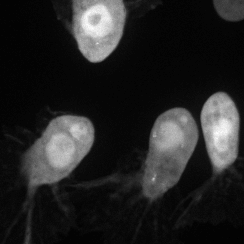
\includegraphics[scale=0.45]{img/fig_quali_tile3.png}
	\end {subfigure}\hspace{0.5cm}
	\begin {subfigure}[b]{0.25\linewidth}
		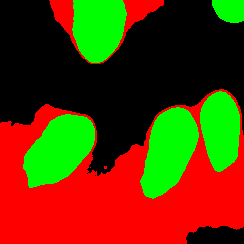
\includegraphics[scale=0.45]{img/fig_quali_tile3_pred_c3.png}
	\end {subfigure}\hspace{0.5cm}
	\begin {subfigure}[b]{0.25\linewidth}
		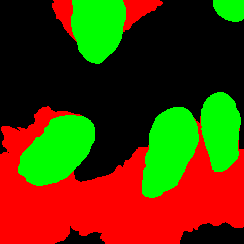
\includegraphics[scale=0.45]{img/fig_quali_tile3_pred_c3_GT.png}
	\end {subfigure}
	\par\medskip
	\begin {subfigure}[b]{0.25\linewidth}
		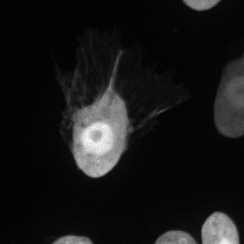
\includegraphics[scale=0.45]{img/fig_quali_tile4.png}
	\end {subfigure}\hspace{0.5cm}
	\begin {subfigure}[b]{0.25\linewidth}
		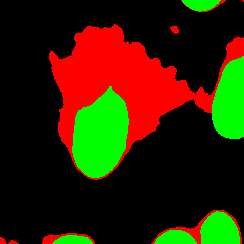
\includegraphics[scale=0.45]{img/fig_quali_tile4_pred_c3.png}
	\end {subfigure}\hspace{0.5cm}
	\begin {subfigure}[b]{0.25\linewidth}
		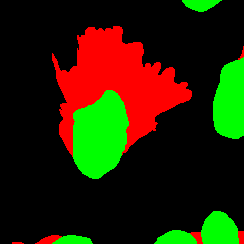
\includegraphics[scale=0.45]{img/fig_quali_tile4_pred_c3_GT.png}
	\end {subfigure}
	\par\bigskip\par\bigskip
	\begin {subfigure}[b]{0.25\linewidth}
		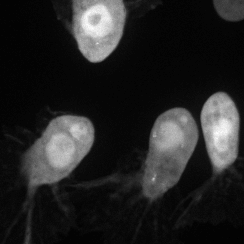
\includegraphics[scale=0.45]{img/fig_quali_tile3.png}
	\end {subfigure}\hspace{0.5cm}
	\begin {subfigure}[b]{0.25\linewidth}
		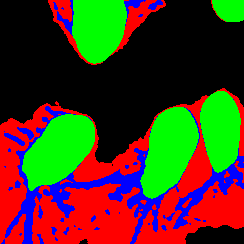
\includegraphics[scale=0.45]{img/fig_quali_tile3_pred_c4.png}
	\end {subfigure}\hspace{0.5cm}
	\begin {subfigure}[b]{0.25\linewidth}
		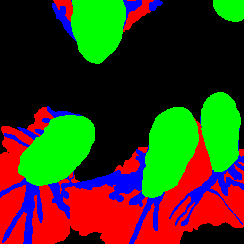
\includegraphics[scale=0.45]{img/fig_quali_tile3_pred_c4_GT.png}
	\end {subfigure}
	\par\medskip
	\begin {subfigure}[b]{0.25\linewidth}
		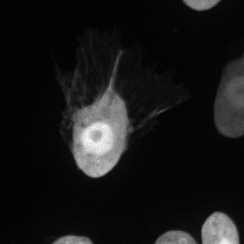
\includegraphics[scale=0.45]{img/fig_quali_tile4.png}
	\end {subfigure}\hspace{0.5cm}
	\begin {subfigure}[b]{0.25\linewidth}
		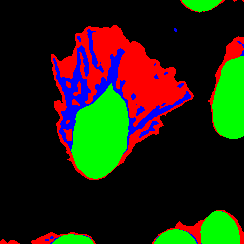
\includegraphics[scale=0.45]{img/fig_quali_tile4_pred_c4.png}
	\end {subfigure}\hspace{0.5cm}
	\begin {subfigure}[b]{0.25\linewidth}
		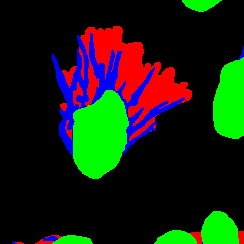
\includegraphics[scale=0.45]{img/fig_quali_tile4_pred_c4_GT.png}
	\end {subfigure}

		\caption[Qualitative prediction results.]{Qualitative results from predicting validation data tiles with the best 3-class network, \textbf{W\_BN\_S\_MS\_LR\_3}, (top two rows) and the best 4-class network, \textbf{W\_BN\_S\_MS\_EL\_4}, (bottom two rows). \textbf{From left to right}: Input image, prediction and image ground truth.}
		\label{fig:qualitative}
\end {figure}